\documentclass[twoside]{book}

% Packages required by doxygen
\usepackage{fixltx2e}
\usepackage{calc}
\usepackage{doxygen}
\usepackage[export]{adjustbox} % also loads graphicx
\usepackage{graphicx}
\usepackage[utf8]{inputenc}
\usepackage{makeidx}
\usepackage{multicol}
\usepackage{multirow}
\PassOptionsToPackage{warn}{textcomp}
\usepackage{textcomp}
\usepackage[nointegrals]{wasysym}
\usepackage[table]{xcolor}

% Font selection
\usepackage[T1]{fontenc}
\usepackage[scaled=.90]{helvet}
\usepackage{courier}
\usepackage{amssymb}
\usepackage{sectsty}
\renewcommand{\familydefault}{\sfdefault}
\allsectionsfont{%
  \fontseries{bc}\selectfont%
  \color{darkgray}%
}
\renewcommand{\DoxyLabelFont}{%
  \fontseries{bc}\selectfont%
  \color{darkgray}%
}
\newcommand{\+}{\discretionary{\mbox{\scriptsize$\hookleftarrow$}}{}{}}

% Page & text layout
\usepackage{geometry}
\geometry{%
  a4paper,%
  top=2.5cm,%
  bottom=2.5cm,%
  left=2.5cm,%
  right=2.5cm%
}
\tolerance=750
\hfuzz=15pt
\hbadness=750
\setlength{\emergencystretch}{15pt}
\setlength{\parindent}{0cm}
\setlength{\parskip}{3ex plus 2ex minus 2ex}
\makeatletter
\renewcommand{\paragraph}{%
  \@startsection{paragraph}{4}{0ex}{-1.0ex}{1.0ex}{%
    \normalfont\normalsize\bfseries\SS@parafont%
  }%
}
\renewcommand{\subparagraph}{%
  \@startsection{subparagraph}{5}{0ex}{-1.0ex}{1.0ex}{%
    \normalfont\normalsize\bfseries\SS@subparafont%
  }%
}
\makeatother

% Headers & footers
\usepackage{fancyhdr}
\pagestyle{fancyplain}
\fancyhead[LE]{\fancyplain{}{\bfseries\thepage}}
\fancyhead[CE]{\fancyplain{}{}}
\fancyhead[RE]{\fancyplain{}{\bfseries\leftmark}}
\fancyhead[LO]{\fancyplain{}{\bfseries\rightmark}}
\fancyhead[CO]{\fancyplain{}{}}
\fancyhead[RO]{\fancyplain{}{\bfseries\thepage}}
\fancyfoot[LE]{\fancyplain{}{}}
\fancyfoot[CE]{\fancyplain{}{}}
\fancyfoot[RE]{\fancyplain{}{\bfseries\scriptsize Generated by Doxygen }}
\fancyfoot[LO]{\fancyplain{}{\bfseries\scriptsize Generated by Doxygen }}
\fancyfoot[CO]{\fancyplain{}{}}
\fancyfoot[RO]{\fancyplain{}{}}
\renewcommand{\footrulewidth}{0.4pt}
\renewcommand{\chaptermark}[1]{%
  \markboth{#1}{}%
}
\renewcommand{\sectionmark}[1]{%
  \markright{\thesection\ #1}%
}

% Indices & bibliography
\usepackage{natbib}
\usepackage[titles]{tocloft}
\setcounter{tocdepth}{3}
\setcounter{secnumdepth}{5}
\makeindex

% Hyperlinks (required, but should be loaded last)
\usepackage{ifpdf}
\ifpdf
  \usepackage[pdftex,pagebackref=true]{hyperref}
\else
  \usepackage[ps2pdf,pagebackref=true]{hyperref}
\fi
\hypersetup{%
  colorlinks=true,%
  linkcolor=blue,%
  citecolor=blue,%
  unicode%
}

% Custom commands
\newcommand{\clearemptydoublepage}{%
  \newpage{\pagestyle{empty}\cleardoublepage}%
}

\usepackage{caption}
\captionsetup{labelsep=space,justification=centering,font={bf},singlelinecheck=off,skip=4pt,position=top}

%===== C O N T E N T S =====

\begin{document}

% Titlepage & ToC
\hypersetup{pageanchor=false,
             bookmarksnumbered=true,
             pdfencoding=unicode
            }
\pagenumbering{alph}
\begin{titlepage}
\vspace*{7cm}
\begin{center}%
{\Large A\+M\+O-\/\+Tools-\/\+Suite \\[1ex]\large v.\+0.\+2.\+14 }\\
\vspace*{1cm}
{\large Generated by Doxygen 1.8.13}\\
\end{center}
\end{titlepage}
\clearemptydoublepage
\pagenumbering{roman}
\tableofcontents
\clearemptydoublepage
\pagenumbering{arabic}
\hypersetup{pageanchor=true}

%--- Begin generated contents ---
\chapter{A\+MO Tools Suite $<$img src=\char`\"{}https\+://img.\+shields.\+io/badge/license-\/\+M\+I\+T-\/blue.\+svg\char`\"{}$>$}
\label{index}\hypertarget{index}{}This is a small, easy-\/to-\/use and fast header-\/only library for reading comma separated value (C\+SV) files.

\subsection*{Features}


\begin{DoxyItemize}
\item Automatically rearranges columns by parsing the header line.
\item Disk I/O and C\+S\+V-\/parsing are overlapped using threads for efficiency.
\item Parsing features such as escaped strings can be enabled and disabled at compile time using templates. You only pay in speed for the features you actually use.
\item Can read multiple GB files in reasonable time.
\item Support for custom columns separators (i.\+e. Tab separated value files are supported), quote escaped strings, automatic space trimming.
\item Works with {\ttfamily $\ast$}nix and Windows newlines and automatically ignores U\+T\+F-\/8 B\+O\+Ms.
\item Exception classes with enough context to format useful error messages. what() returns error messages ready to be shown to a user.
\end{DoxyItemize}

\subsection*{Getting Started}

The following small example should contain most of the syntax you need to use the library.


\begin{DoxyCode}
\textcolor{preprocessor}{# include "csv.h"}

\textcolor{keywordtype}{int} main()\{
  \hyperlink{classio_1_1_c_s_v_reader}{io::CSVReader<3>} in(\textcolor{stringliteral}{"ram.csv"});
  in.read\_header(io::ignore\_extra\_column, \textcolor{stringliteral}{"vendor"}, \textcolor{stringliteral}{"size"}, \textcolor{stringliteral}{"speed"});
  std::string vendor; \textcolor{keywordtype}{int} size; \textcolor{keywordtype}{double} speed;
  \textcolor{keywordflow}{while}(in.read\_row(vendor, size, speed))\{
    \textcolor{comment}{// do stuff with the data}
  \}
\}
\end{DoxyCode}


\subsection*{Installation}

The library only needs a standard conformant C++11 compiler. It has no further dependencies. The library is completely contained inside a single header file and therefore it is sufficient to copy this file to some place on your include path. The library does not have to be explicitly build.

Note however, that threads are used and some compiler (for example G\+CC) require you to link against additional librarie to make it work. With G\+CC it is important to add -\/lpthread as the last item when linking, i.\+e. the order in


\begin{DoxyCode}
g++ -std=c++0x a.o b.o -o prog -lpthread
\end{DoxyCode}


is important. If you for some reason do not want to use threads you can define C\+S\+V\+\_\+\+I\+O\+\_\+\+N\+O\+\_\+\+T\+H\+R\+E\+AD before including the header.

Remember that the library makes use of C++11 features and therefore you have to enable support for it (f.\+e. add -\/std=c++0x or -\/std=gnu++0x).

The library was developed and tested with G\+CC 4.\+6.\+1

Note that V\+S2013 is not C++11 compilant and will therefore not work out of the box. See \href{https://code.google.com/p/fast-cpp-csv-parser/issues/detail?id=6}{\tt here} for what needs to be adjusted to make the code work.

\subsection*{Documentation}

The libary provides two classes\+:


\begin{DoxyItemize}
\item {\ttfamily Line\+Reader}\+: A class to efficiently read large files line by line.
\item {\ttfamily C\+S\+V\+Reader}\+: A class that efficiently reads large C\+SV files.
\end{DoxyItemize}

Note that everything is contained in the {\ttfamily io} namespace.

\subsubsection*{{\ttfamily Line\+Reader}}


\begin{DoxyCode}
\textcolor{keyword}{class }LineReader\{
\textcolor{keyword}{public}:
  \textcolor{comment}{// Constructors}
  LineReader(some\_string\_type file\_name);
  LineReader(some\_string\_type file\_name, std::FILE*source);
  LineReader(some\_string\_type file\_name, std::istream&source);
  LineReader(some\_string\_type file\_name, std::unique\_ptr<ByteSourceBase>source);

  \textcolor{comment}{// Reading}
  \textcolor{keywordtype}{char}*next\_line();

  \textcolor{comment}{// File Location}
  \textcolor{keywordtype}{void} set\_file\_line(\textcolor{keywordtype}{unsigned});
  \textcolor{keywordtype}{unsigned} get\_file\_line()\textcolor{keyword}{const};
  \textcolor{keywordtype}{void} set\_file\_name(some\_string\_type file\_name);
  \textcolor{keyword}{const} \textcolor{keywordtype}{char}*get\_truncated\_file\_name()\textcolor{keyword}{const};
\};
\end{DoxyCode}


The constructor takes a file name and optionally a data source. If no data source is provided the function tries to open the file with the given name and throws an {\ttfamily error\+::can\+\_\+not\+\_\+open\+\_\+file exception} on failure. If a data source is provided then the file name is only used to format error messages. In that case you can essentially put any string there. Using a string that describes the data source results in more informative error messages.

{\ttfamily some\+\_\+string\+\_\+type} can be a {\ttfamily std\+::string} or a {\ttfamily char$\ast$}. If the data source is a {\ttfamily std\+::\+F\+I\+LE$\ast$} then the library will take care of calling {\ttfamily std\+::fclose}. If it is a {\ttfamily std\+::istream} then the stream is not closed by the library. For best performance open the streams in binary mode. However using text mode also works. {\ttfamily Byte\+Source\+Base} provides an interface that you can use to implement further data sources.


\begin{DoxyCode}
\textcolor{keyword}{class }ByteSourceBase\{
\textcolor{keyword}{public}:
  \textcolor{keyword}{virtual} \textcolor{keywordtype}{int} read(\textcolor{keywordtype}{char}*buffer, \textcolor{keywordtype}{int} size)=0;
  \textcolor{keyword}{virtual} ~ByteSourceBase()\{\}
\};
\end{DoxyCode}


The read function should fill the provided buffer with at most {\ttfamily size} bytes from the data source. It should return the number of bytes actually written to the buffer. If data source has run out of bytes (because for example an end of file was reached) then the function should return 0. If a fatal error occures then you can throw an exception. Note that the function can be called both from the main and the worker thread. However, it is guarenteed that they do not call the function at the same time.

Lines are read by calling the {\ttfamily next\+\_\+line} function. It returns a pointer to a null terminated C-\/string that contains the line. If the end of file is reached a null pointer is returned. The newline character is not included in the string. You may modify the string as long as you do not write past the null terminator. The string stays valid until the destructor is called or until next\+\_\+line is called again. Windows and {\ttfamily $\ast$}nix newlines are handled transparently. U\+T\+F-\/8 B\+O\+Ms are automatically ignored and missing newlines at the end of the file are no problem.

{\bfseries Important\+:} There is a limit of 2$^\wedge$24-\/1 characters per line. If this limit is exceeded a {\ttfamily error\+::line\+\_\+length\+\_\+limit\+\_\+exceeded} exception is thrown.

Looping over all the lines in a file can be done in the following way. 
\begin{DoxyCode}
LineReader in(...);
\textcolor{keywordflow}{while}(\textcolor{keywordtype}{char}*line = in.next\_line())\{
  ...
\}
\end{DoxyCode}


The remaining functions are mainly used used to format error messages. The file line indicates the current position in the file, i.\+e., after the first {\ttfamily next\+\_\+line} call it is 1 and after the second 2. Before the first call it is 0. The file name is truncated as internally C-\/strings are used to avoid {\ttfamily std\+::bad\+\_\+alloc} exceptions during error reporting.

{\bfseries Note\+:} It is not possible to exchange the line termination character.

\subsubsection*{{\ttfamily C\+S\+V\+Reader}}

{\ttfamily C\+S\+V\+Reader} uses policies. These are classes with only static members to allow core functionality to be exchanged in an efficient way.


\begin{DoxyCode}
\textcolor{keyword}{template}<
  \textcolor{keywordtype}{unsigned} column\_count,
  \textcolor{keyword}{class }trim\_policy = trim\_chars<' ', '\(\backslash\)t'>, 
  \textcolor{keyword}{class }quote\_policy = no\_quote\_escape<','>,
  \textcolor{keyword}{class }overflow\_policy = throw\_on\_overflow,
  \textcolor{keyword}{class }comment\_policy = no\_comment
>
\textcolor{keyword}{class }CSVReader\{
\textcolor{keyword}{public}:
  \textcolor{comment}{// Constructors}
  \textcolor{comment}{// same as for LineReader}

  \textcolor{comment}{// Parsing Header}
  \textcolor{keywordtype}{void} read\_header(ignore\_column ignore\_policy, some\_string\_type col\_name1, some\_string\_type col\_name2, ...
      );
  \textcolor{keywordtype}{void} set\_header(some\_string\_type col\_name1, some\_string\_type col\_name2, ...);
  \textcolor{keywordtype}{bool} has\_column(some\_string\_type col\_name)\textcolor{keyword}{const};

  \textcolor{comment}{// Read}
  \textcolor{keywordtype}{char}*next\_line();
  \textcolor{keywordtype}{bool} read\_row(ColType1&col1, ColType2&col2, ...);

  \textcolor{comment}{// File Location }
  \textcolor{keywordtype}{void} set\_file\_line(\textcolor{keywordtype}{unsigned});
  \textcolor{keywordtype}{unsigned} get\_file\_line()\textcolor{keyword}{const};
  \textcolor{keywordtype}{void} set\_file\_name(some\_string\_type file\_name);
  \textcolor{keyword}{const} \textcolor{keywordtype}{char}*get\_truncated\_file\_name()\textcolor{keyword}{const};
\};
\end{DoxyCode}


The {\ttfamily column\+\_\+count} template parameter indicates how many columns you want to read from the C\+SV file. This must not necessarily coincide with the actual number of columns in the file. The three policies govern various aspects of the parsing.

The trim policy indicates what characters should be ignored at the begin and the end of every column. The default ignores spaces and tabs. This makes sure that


\begin{DoxyCode}
a,b,c
1,2,3
\end{DoxyCode}


is interpreted in the same way as


\begin{DoxyCode}
  a, b,   c
1  , 2,   3
\end{DoxyCode}


The trim\+\_\+chars can take any number of template parameters. For example `trim\+\_\+chars$<$\textquotesingle{} \textquotesingle{}, \textquotesingle{}\textquotesingle{}, \textquotesingle{}\+\_\+\textquotesingle{}$>$ {\ttfamily is also valid. If no character should be trimmed use}trim\+\_\+chars$<$$>$`.

The quote policy indicates how string should be escaped. It also specifies the column separator. The predefined policies are\+:


\begin{DoxyItemize}
\item {\ttfamily no\+\_\+quote\+\_\+escape$<$sep$>$} \+: Strings are not escaped. \char`\"{}`sep`\char`\"{} is used as column separator.
\item {\ttfamily double\+\_\+quote\+\_\+escape$<$sep, quote$>$} \+: Strings are escaped using quotes. Quotes are escaped using two consecutive quotes. \char`\"{}`sep`\char`\"{} is used as column separator and \char`\"{}`quote`\char`\"{} as quoting character.
\end{DoxyItemize}

{\bfseries Important}\+: When combining trimming and quoting the rows are first trimmed and then unquoted. A consequence is that spaces inside the quotes will be conserved. If you want to get rid of spaces inside the quotes, you need to remove them yourself.

{\bfseries Important}\+: Quoting can be quite expensive. Disable it if you do not need it.

The overflow policy indicates what should be done if the integers in the input are too large to fit into the variables. There following policies are predefined\+:


\begin{DoxyItemize}
\item {\ttfamily throw\+\_\+on\+\_\+overflow} \+: Throw an {\ttfamily error\+::integer\+\_\+overflow} or {\ttfamily error\+::integer\+\_\+underflow} exception.
\item {\ttfamily ignore\+\_\+overflow} \+: Do nothing and let the overflow happen.
\item {\ttfamily set\+\_\+to\+\_\+max\+\_\+on\+\_\+overflow} \+: Set the value to {\ttfamily numeric\+\_\+limits$<$...$>$\+::max()} (or to the min-\/pendant).
\end{DoxyItemize}

The comment policy allows to skip lines based on some criteria. Valid predefined policies are\+:


\begin{DoxyItemize}
\item {\ttfamily no\+\_\+comment} \+: Do not ignore any line.
\item {\ttfamily empty\+\_\+line\+\_\+comment} \+: Ignore all lines that are empty or only contains spaces and tabs.
\item {\ttfamily single\+\_\+line\+\_\+comment$<$com1, com2, ...$>$} \+: Ignore all lines that start with com1 or com2 or ... as the first character. There may not be any space between the beginning of the line and the comment character.
\item {\ttfamily single\+\_\+and\+\_\+empty\+\_\+line\+\_\+comment$<$com1, com2, ...$>$} \+: Ignore all empty lines and single line comments.
\end{DoxyItemize}

Examples\+:


\begin{DoxyItemize}
\item `\+C\+S\+V\+Reader$<$4, trim\+\_\+chars$<$\textquotesingle{} \textquotesingle{}$>$, double\+\_\+quote\+\_\+escape$<$\textquotesingle{},\textquotesingle{},\textquotesingle{}"\textquotesingle{}$>$ $>${\ttfamily reads 4 columns from a normal C\+SV file with string escaping enabled. $\ast$}C\+S\+V\+Reader$<$3, trim\+\_\+chars$<$\textquotesingle{} \textquotesingle{}$>$, no\+\_\+quote\+\_\+escape$<$\textquotesingle{}\textquotesingle{}$>$, single\+\_\+line\+\_\+comment$<$\textquotesingle{}\#\textquotesingle{}$>$ $>$` reads 3 columns from a tab separated file with string escaping disabled. Lines starting with a \# are ignored.
\end{DoxyItemize}

The constructors and the file location functions are exactly the same as for {\ttfamily Line\+Reader}. See its documentation for details.

There are three methods that deal with headers. The {\ttfamily read\+\_\+header} methods reads a line from the file and rearranges the columns to match that order. It also checks whether all necessary columns are present. The {\ttfamily set\+\_\+header} method does {\itshape not} read any input. Use it if the file does not have any header. Obviously it is impossible to rearrange columns or check for their availability when using it. The order in the file and in the program must match when using {\ttfamily set\+\_\+header}. The {\ttfamily has\+\_\+column} method checks whether a column is present in the file. The first argument of {\ttfamily read\+\_\+header} is a bitfield that determines how the function should react to column mismatches. The default behavior is to throw an {\ttfamily error\+::extra\+\_\+column\+\_\+in\+\_\+header} exception if the file contains more columns than expected and an {\ttfamily error\+::missing\+\_\+column\+\_\+in\+\_\+header} when there are not enough. This behavior can be altered using the following flags.


\begin{DoxyItemize}
\item {\ttfamily ignore\+\_\+no\+\_\+column}\+: The default behavior, no flags are set
\item {\ttfamily ignore\+\_\+extra\+\_\+column}\+: If a column with a name is in the file but not in the argument list, then it is silently ignored.
\item {\ttfamily ignore\+\_\+missing\+\_\+column}\+: If a column with a name is not in the file but is in the argument list, then {\ttfamily read\+\_\+row} will not modify the corresponding variable.
\end{DoxyItemize}

When using {\ttfamily ignore\+\_\+column\+\_\+missing} it is a good idea to initialize the variables passed to {\ttfamily read\+\_\+row} with a default value, for example\+:


\begin{DoxyCode}
\textcolor{comment}{// The file only contains column "a"}
CSVReader<2>in(...);
in.read\_header(ignore\_missing\_column, \textcolor{stringliteral}{"a"}, \textcolor{stringliteral}{"b"});
\textcolor{keywordtype}{int} a,b = 42;
\textcolor{keywordflow}{while}(in.read\_row(a,b))\{
  \textcolor{comment}{// a contains the value from the file}
  \textcolor{comment}{// b is left unchanged by read\_row, i.e., it is 42}
\}
\end{DoxyCode}


If only some columns are optional or their default value depends on other columns you have to use {\ttfamily has\+\_\+column}, for example\+:


\begin{DoxyCode}
\textcolor{comment}{// The file only contains the columns "a" and "b"}
CSVReader<2>in(...);
in.read\_header(ignore\_missing\_column, \textcolor{stringliteral}{"a"}, \textcolor{stringliteral}{"b"}, \textcolor{stringliteral}{"sum"});
\textcolor{keywordflow}{if}(!in.has\_column(\textcolor{stringliteral}{"a"}) || !in.has\_column(\textcolor{stringliteral}{"b"}))
  \textcolor{keywordflow}{throw} my\_neat\_error\_class();
\textcolor{keywordtype}{bool} has\_sum = in.has\_column(\textcolor{stringliteral}{"sum"});
\textcolor{keywordtype}{int} a,b,sum;
\textcolor{keywordflow}{while}(in.read\_row(a,b,sum))\{
  \textcolor{keywordflow}{if}(!has\_sum)
    sum = a+b;
\}
\end{DoxyCode}


{\bfseries Important}\+: Do not call {\ttfamily has\+\_\+column} from within the read-\/loop. It would work correctly but significantly slowdown processing.

If two columns have the same name an error\+::duplicated\+\_\+column\+\_\+in\+\_\+header exception is thrown. If {\ttfamily read\+\_\+header} is called but the file is empty a {\ttfamily error\+::header\+\_\+missing} exception is thrown.

The {\ttfamily next\+\_\+line} functions reads a line without parsing it. It works analogous to {\ttfamily Line\+Reader\+::next\+\_\+line}. This can be used to skip broken lines in a C\+SV file. However, in nearly all applications you will want to use the {\ttfamily read\+\_\+row} function.

The {\ttfamily read\+\_\+row} function reads a line, splits it into the columns and arranges them correctly. It trims the entries and unescapes them. If requested the content is interpreted as integer or as floating point. The variables passed to read\+\_\+row may be of the following types.


\begin{DoxyItemize}
\item builtin signed integer\+: These are {\ttfamily signed char}, {\ttfamily short}, {\ttfamily int}, {\ttfamily long} and {\ttfamily long long}. The input must be encoded as a base 10 A\+S\+C\+II number optionally preceded by a + or -\/. The function detects whether the integer is too large would overflow (or underflow) and behaves as indicated by overflow\+\_\+policy.
\item builtin unsigned integer\+: Just as the signed counterparts except that a leading + or -\/ is not allowed.
\item builtin floating point\+: These are {\ttfamily float}, {\ttfamily double} and {\ttfamily long double}. The input may have a leading + or -\/. The number must be base 10 encoded. The decimal point may either be a dot or a comma. (Note that a comma will only work if it is not also used as column separator or the number is escaped.) A base 10 exponent may be specified using the \char`\"{}1e10\char`\"{} syntax. The \char`\"{}e\char`\"{} may be lower-\/ or uppercase. Examples for valid floating points are \char`\"{}1\char`\"{}, \char`\"{}-\/42.\+42\char`\"{} and \char`\"{}+123.\+456\+E789\char`\"{}. The input is rounded to the next floating point or infinity if it is too large or small.
\item {\ttfamily char}\+: The column content must be a single character.
\item {\ttfamily std\+::string}\+: The column content is assigned to the string. The std\+::string is filled with the trimmed and unescaped version.
\item {\ttfamily char$\ast$}\+: A pointer directly into the buffer. The string is trimmed and unescaped and null terminated. This pointer stays valid until read\+\_\+row is called again or the C\+S\+V\+Reader is destroyed. Use this for user defined types.
\end{DoxyItemize}

Note that there is no inherent overhead to using {\ttfamily char$\ast$} and then interpreting it compared to using one of the parsers directly build into {\ttfamily C\+S\+V\+Reader}. The builtin number parsers are pure convenience. If you need a slightly different syntax then use {\ttfamily char$\ast$} and do the parsing yourself.

\subsection*{F\+AQ}

Q\+: The library is throwing a std\+::system\+\_\+error with code -\/1. How to get it to work?

A\+: Your compiler\textquotesingle{}s std\+::thread implementation is broken. Define C\+S\+V\+\_\+\+I\+O\+\_\+\+N\+O\+\_\+\+T\+H\+R\+E\+AD to disable threading support.

Q\+: My values are not just ints or strings. I want to parse my customized type. Is this possible?

A\+: Read a {\ttfamily char$\ast$} and parse the string. At first this seems expensive but it is not as the pointer you get points directly into the memory buffer. In fact there is no inherent reason why a custom int-\/parser realized this way must be any slower than the int-\/parser build into the library. By reading a {\ttfamily char$\ast$} the library takes care of column reordering and quote escaping and leaves the actual parsing to you. Note that using a std\+::string is slower as it involves a memory copy.

Q\+: I get lots of compiler errors when compiling the header! Please fix it. \+:(

A\+: Have you enabled the C++11 mode of your compiler? If you use G\+CC you have to add -\/std=c++0x to the commandline. If this does not resolve the problem, then please open a ticket.

Q\+: The library crashes when parsing large files! Please fix it. \+:(

A\+: When using G\+CC have you linked against -\/lpthread? Read the installation section for details on how to do this. If this does not resolve the issue then please open a ticket. (The reason why it only crashes only on large files is that the first chuck is read synchronous and if the whole file fits into this chuck then no asynchronous call is performed.) Alternatively you can define C\+S\+V\+\_\+\+I\+O\+\_\+\+N\+O\+\_\+\+T\+H\+R\+E\+AD.

Q\+: Does the library support U\+TF?

A\+: The library has basic U\+T\+F-\/8 support, or to be more precise it does not break when passing U\+T\+F-\/8 strings through it. If you read a {\ttfamily char$\ast$} then you get a pointer to the U\+T\+F-\/8 string. You will have to decode the string on your own. The separator, quoting, and commenting characters used by the library can only be A\+S\+C\+II characters. 
\chapter{Hierarchical Index}
\section{Class Hierarchy}
This inheritance list is sorted roughly, but not completely, alphabetically\+:\begin{DoxyCompactList}
\item \contentsline{section}{Compressor\+:\+:Air\+System\+Capacity}{\pageref{class_compressor_1_1_air_system_capacity}}{}
\item \contentsline{section}{Compressor\+:\+:Air\+Velocity}{\pageref{class_compressor_1_1_air_velocity}}{}
\item \contentsline{section}{Annual\+Cost}{\pageref{class_annual_cost}}{}
\item \contentsline{section}{Annual\+Energy}{\pageref{class_annual_energy}}{}
\item \contentsline{section}{Atmosphere}{\pageref{class_atmosphere}}{}
\item \contentsline{section}{Auxiliary\+Power}{\pageref{class_auxiliary_power}}{}
\item \contentsline{section}{Bag\+Method}{\pageref{class_bag_method}}{}
\item \contentsline{section}{Fan\+Curve\+Data\+:\+:Base\+Curve}{\pageref{struct_fan_curve_data_1_1_base_curve}}{}
\begin{DoxyCompactList}
\item \contentsline{section}{Fan\+Curve\+Data\+:\+:Rated\+Point}{\pageref{struct_fan_curve_data_1_1_rated_point}}{}
\begin{DoxyCompactList}
\item \contentsline{section}{Fan\+Curve\+Data\+:\+:Base\+Operating\+Point}{\pageref{struct_fan_curve_data_1_1_base_operating_point}}{}
\end{DoxyCompactList}
\end{DoxyCompactList}
\item \contentsline{section}{Base\+Gas\+Density}{\pageref{class_base_gas_density}}{}
\item \contentsline{section}{Boiler}{\pageref{class_boiler}}{}
\item \contentsline{section}{C\+HP}{\pageref{class_c_h_p}}{}
\item \contentsline{section}{Curve\+Fit\+Val}{\pageref{class_curve_fit_val}}{}
\item \contentsline{section}{Plane\+Data\+:\+:Node\+Binding\+:\+:Data}{\pageref{struct_plane_data_1_1_node_binding_1_1_data}}{}
\begin{DoxyCompactList}
\item \contentsline{section}{Plane\+Data\+:\+:Node\+Binding\+:\+:Data\+Flange}{\pageref{struct_plane_data_1_1_node_binding_1_1_data_flange}}{}
\end{DoxyCompactList}
\item \contentsline{section}{Deaerator}{\pageref{class_deaerator}}{}
\item \contentsline{section}{Efficiency\+Improvement}{\pageref{class_efficiency_improvement}}{}
\item \contentsline{section}{Electrical\+Energy\+Equivalency}{\pageref{class_electrical_energy_equivalency}}{}
\item \contentsline{section}{Energy\+Input\+E\+AF}{\pageref{class_energy_input_e_a_f}}{}
\item \contentsline{section}{Energy\+Input\+Exhaust\+Gas\+Losses}{\pageref{class_energy_input_exhaust_gas_losses}}{}
\item \contentsline{section}{Estimate\+F\+LA}{\pageref{class_estimate_f_l_a}}{}
\item \contentsline{section}{Exhaust\+Gas\+E\+AF}{\pageref{class_exhaust_gas_e_a_f}}{}
\item \contentsline{section}{Fan}{\pageref{class_fan}}{}
\item \contentsline{section}{Fan\+Curve}{\pageref{class_fan_curve}}{}
\item \contentsline{section}{Fan\+Curve\+Data}{\pageref{class_fan_curve_data}}{}
\item \contentsline{section}{Fan\+Rated\+Info}{\pageref{class_fan_rated_info}}{}
\item \contentsline{section}{Fan\+:\+:Fan\+Results}{\pageref{struct_fan_1_1_fan_results}}{}
\item \contentsline{section}{Fan\+Shaft\+Power}{\pageref{class_fan_shaft_power}}{}
\item \contentsline{section}{Field\+Data}{\pageref{class_field_data}}{}
\item \contentsline{section}{Financial}{\pageref{class_financial}}{}
\item \contentsline{section}{Fixture\+Losses}{\pageref{class_fixture_losses}}{}
\item \contentsline{section}{Flash\+Tank}{\pageref{class_flash_tank}}{}
\item \contentsline{section}{Flow\+Calculations\+Energy\+Use}{\pageref{class_flow_calculations_energy_use}}{}
\item \contentsline{section}{Fluid\+Power}{\pageref{class_fluid_power}}{}
\item \contentsline{section}{Fuel\+Fired\+Energy\+Equivalency}{\pageref{class_fuel_fired_energy_equivalency}}{}
\item \contentsline{section}{Gas\+Compositions}{\pageref{class_gas_compositions}}{}
\item \contentsline{section}{Gas\+Cooling\+Losses}{\pageref{class_gas_cooling_losses}}{}
\item \contentsline{section}{Gas\+Flue\+Gas\+Material}{\pageref{class_gas_flue_gas_material}}{}
\item \contentsline{section}{Gas\+Load\+Charge\+Material}{\pageref{class_gas_load_charge_material}}{}
\item \contentsline{section}{Gas\+Properties}{\pageref{class_gas_properties}}{}
\item \contentsline{section}{Header}{\pageref{class_header}}{}
\item \contentsline{section}{Head\+Tool\+Base}{\pageref{class_head_tool_base}}{}
\begin{DoxyCompactList}
\item \contentsline{section}{Head\+Tool}{\pageref{class_head_tool}}{}
\item \contentsline{section}{Head\+Tool\+Suction\+Tank}{\pageref{class_head_tool_suction_tank}}{}
\end{DoxyCompactList}
\item \contentsline{section}{Heat\+Loss}{\pageref{class_heat_loss}}{}
\item \contentsline{section}{Humidity\+Ratio}{\pageref{class_humidity_ratio}}{}
\item \contentsline{section}{Inlet}{\pageref{class_inlet}}{}
\item \contentsline{section}{Leakage\+Losses}{\pageref{class_leakage_losses}}{}
\item \contentsline{section}{Liquid\+Cooling\+Losses}{\pageref{class_liquid_cooling_losses}}{}
\item \contentsline{section}{Liquid\+Load\+Charge\+Material}{\pageref{class_liquid_load_charge_material}}{}
\item \contentsline{section}{Motor}{\pageref{class_motor}}{}
\item \contentsline{section}{Motor\+Current}{\pageref{class_motor_current}}{}
\item \contentsline{section}{Motor\+Data}{\pageref{class_motor_data}}{}
\item \contentsline{section}{Motor\+Efficiency}{\pageref{class_motor_efficiency}}{}
\item \contentsline{section}{Motor\+Power}{\pageref{class_motor_power}}{}
\item \contentsline{section}{Motor\+Power\+Factor}{\pageref{class_motor_power_factor}}{}
\item \contentsline{section}{Motor\+Shaft\+Power}{\pageref{class_motor_shaft_power}}{}
\item \contentsline{section}{Plane\+Data\+:\+:Node\+Binding}{\pageref{struct_plane_data_1_1_node_binding}}{}
\item \contentsline{section}{O2\+Enrichment}{\pageref{class_o2_enrichment}}{}
\item \contentsline{section}{Opening\+Losses}{\pageref{class_opening_losses}}{}
\item \contentsline{section}{Compressor\+:\+:Operating\+Cost}{\pageref{class_compressor_1_1_operating_cost}}{}
\item \contentsline{section}{Optimal\+Deviation\+Factor}{\pageref{class_optimal_deviation_factor}}{}
\item \contentsline{section}{Optimal\+Motor\+Power}{\pageref{class_optimal_motor_power}}{}
\item \contentsline{section}{Optimal\+Motor\+Shaft\+Power}{\pageref{class_optimal_motor_shaft_power}}{}
\item \contentsline{section}{Optimal\+Motor\+Size}{\pageref{class_optimal_motor_size}}{}
\item \contentsline{section}{Optimal\+Pre\+Pump\+Eff}{\pageref{class_optimal_pre_pump_eff}}{}
\item \contentsline{section}{Optimal\+Pump\+Efficiency}{\pageref{class_optimal_pump_efficiency}}{}
\item \contentsline{section}{Optimal\+Pump\+Shaft\+Power}{\pageref{class_optimal_pump_shaft_power}}{}
\item \contentsline{section}{Optimal\+Specific\+Speed}{\pageref{class_optimal_specific_speed}}{}
\item \contentsline{section}{Optimal\+Specific\+Speed\+Correction}{\pageref{class_optimal_specific_speed_correction}}{}
\item \contentsline{section}{Bag\+Method\+:\+:Output}{\pageref{struct_bag_method_1_1_output}}{}
\item \contentsline{section}{Plane\+Data\+:\+:Node\+Binding\+:\+:Output}{\pageref{struct_plane_data_1_1_node_binding_1_1_output}}{}
\item \contentsline{section}{Compressor\+:\+:Pipe\+Sizing\+:\+:Output}{\pageref{struct_compressor_1_1_pipe_sizing_1_1_output}}{}
\item \contentsline{section}{Pneumatic\+Air\+Requirement\+:\+:Output}{\pageref{class_pneumatic_air_requirement_1_1_output}}{}
\item \contentsline{section}{Compressor\+:\+:Operating\+Cost\+:\+:Output}{\pageref{struct_compressor_1_1_operating_cost_1_1_output}}{}
\item \contentsline{section}{Compressor\+:\+:Air\+System\+Capacity\+:\+:Output}{\pageref{struct_compressor_1_1_air_system_capacity_1_1_output}}{}
\item \contentsline{section}{Compressor\+:\+:Pipe\+Data}{\pageref{struct_compressor_1_1_pipe_data}}{}
\item \contentsline{section}{Compressor\+:\+:Pipe\+Sizing}{\pageref{class_compressor_1_1_pipe_sizing}}{}
\item \contentsline{section}{Planar}{\pageref{class_planar}}{}
\begin{DoxyCompactList}
\item \contentsline{section}{Flange\+Plane}{\pageref{class_flange_plane}}{}
\item \contentsline{section}{Mst\+Plane}{\pageref{class_mst_plane}}{}
\item \contentsline{section}{Traverse\+Plane}{\pageref{class_traverse_plane}}{}
\end{DoxyCompactList}
\item \contentsline{section}{Plane\+Data}{\pageref{class_plane_data}}{}
\item \contentsline{section}{Pneumatic\+Air\+Requirement}{\pageref{class_pneumatic_air_requirement}}{}
\item \contentsline{section}{Compressor\+:\+:Pneumatic\+Valve}{\pageref{class_compressor_1_1_pneumatic_valve}}{}
\item \contentsline{section}{Point}{\pageref{class_point}}{}
\item \contentsline{section}{Poles}{\pageref{class_poles}}{}
\item \contentsline{section}{Prv\+With\+Desuperheating}{\pageref{class_prv_with_desuperheating}}{}
\item \contentsline{section}{Prv\+Without\+Desuperheating}{\pageref{class_prv_without_desuperheating}}{}
\item \contentsline{section}{P\+S\+A\+T\+Result}{\pageref{class_p_s_a_t_result}}{}
\item \contentsline{section}{Pump}{\pageref{class_pump}}{}
\item \contentsline{section}{Pump\+Efficiency}{\pageref{class_pump_efficiency}}{}
\item \contentsline{section}{Pump\+Shaft\+Power}{\pageref{class_pump_shaft_power}}{}
\item \contentsline{section}{Receiver\+Tank}{\pageref{class_receiver_tank}}{}
\item \contentsline{section}{P\+S\+A\+T\+Result\+:\+:result}{\pageref{struct_p_s_a_t_result_1_1result}}{}
\item \contentsline{section}{Result\+Data}{\pageref{class_result_data}}{}
\item \contentsline{section}{Saturated\+Pressure}{\pageref{class_saturated_pressure}}{}
\item \contentsline{section}{Saturated\+Properties}{\pageref{class_saturated_properties}}{}
\item \contentsline{section}{Saturated\+Temperature}{\pageref{class_saturated_temperature}}{}
\item \contentsline{section}{Slag\+Other\+Material\+Losses}{\pageref{class_slag_other_material_losses}}{}
\item \contentsline{section}{Solid\+Liquid\+Flue\+Gas\+Material}{\pageref{class_solid_liquid_flue_gas_material}}{}
\item \contentsline{section}{Solid\+Load\+Charge\+Material}{\pageref{class_solid_load_charge_material}}{}
\item \contentsline{section}{S\+Q\+Lite\+Wrapper}{\pageref{class_s_q_lite_wrapper}}{}
\begin{DoxyCompactList}
\item \contentsline{section}{S\+Q\+Lite}{\pageref{class_s_q_lite}}{}
\end{DoxyCompactList}
\item \contentsline{section}{Steam\+Properties}{\pageref{class_steam_properties}}{}
\item \contentsline{section}{Steam\+System\+Modeler\+Tool}{\pageref{class_steam_system_modeler_tool}}{}
\item \contentsline{section}{Turbine}{\pageref{class_turbine}}{}
\item \contentsline{section}{Velocity\+Pressure\+Traverse\+Data}{\pageref{class_velocity_pressure_traverse_data}}{}
\begin{DoxyCompactList}
\item \contentsline{section}{Traverse\+Plane}{\pageref{class_traverse_plane}}{}
\end{DoxyCompactList}
\item \contentsline{section}{Wall\+Losses}{\pageref{class_wall_losses}}{}
\item \contentsline{section}{Water\+Cooling\+Losses}{\pageref{class_water_cooling_losses}}{}
\end{DoxyCompactList}

\chapter{Class Index}
\section{Class List}
Here are the classes, structs, unions and interfaces with brief descriptions\+:\begin{DoxyCompactList}
\item\contentsline{section}{\hyperlink{class_compressor_1_1_air_system_capacity}{Compressor\+::\+Air\+System\+Capacity} }{\pageref{class_compressor_1_1_air_system_capacity}}{}
\item\contentsline{section}{\hyperlink{class_compressor_1_1_air_velocity}{Compressor\+::\+Air\+Velocity} }{\pageref{class_compressor_1_1_air_velocity}}{}
\item\contentsline{section}{\hyperlink{class_annual_cost}{Annual\+Cost} \\*\hyperlink{class_header}{Header} file for \hyperlink{class_annual_cost}{Annual\+Cost} class }{\pageref{class_annual_cost}}{}
\item\contentsline{section}{\hyperlink{class_annual_energy}{Annual\+Energy} \\*Function prototypes for the Annual Energy }{\pageref{class_annual_energy}}{}
\item\contentsline{section}{\hyperlink{class_atmosphere}{Atmosphere} }{\pageref{class_atmosphere}}{}
\item\contentsline{section}{\hyperlink{class_auxiliary_power}{Auxiliary\+Power} }{\pageref{class_auxiliary_power}}{}
\item\contentsline{section}{\hyperlink{class_bag_method}{Bag\+Method} }{\pageref{class_bag_method}}{}
\item\contentsline{section}{\hyperlink{struct_fan_curve_data_1_1_base_curve}{Fan\+Curve\+Data\+::\+Base\+Curve} }{\pageref{struct_fan_curve_data_1_1_base_curve}}{}
\item\contentsline{section}{\hyperlink{class_base_gas_density}{Base\+Gas\+Density} }{\pageref{class_base_gas_density}}{}
\item\contentsline{section}{\hyperlink{struct_fan_curve_data_1_1_base_operating_point}{Fan\+Curve\+Data\+::\+Base\+Operating\+Point} }{\pageref{struct_fan_curve_data_1_1_base_operating_point}}{}
\item\contentsline{section}{\hyperlink{class_boiler}{Boiler} }{\pageref{class_boiler}}{}
\item\contentsline{section}{\hyperlink{class_c_h_p}{C\+HP} }{\pageref{class_c_h_p}}{}
\item\contentsline{section}{\hyperlink{class_compressibility_factor}{Compressibility\+Factor} }{\pageref{class_compressibility_factor}}{}
\item\contentsline{section}{\hyperlink{class_curve_fit_val}{Curve\+Fit\+Val} \\*Curve Fit class }{\pageref{class_curve_fit_val}}{}
\item\contentsline{section}{\hyperlink{struct_plane_data_1_1_node_binding_1_1_data}{Plane\+Data\+::\+Node\+Binding\+::\+Data} }{\pageref{struct_plane_data_1_1_node_binding_1_1_data}}{}
\item\contentsline{section}{\hyperlink{struct_plane_data_1_1_node_binding_1_1_data_flange}{Plane\+Data\+::\+Node\+Binding\+::\+Data\+Flange} }{\pageref{struct_plane_data_1_1_node_binding_1_1_data_flange}}{}
\item\contentsline{section}{\hyperlink{class_deaerator}{Deaerator} }{\pageref{class_deaerator}}{}
\item\contentsline{section}{\hyperlink{class_efficiency_improvement}{Efficiency\+Improvement} }{\pageref{class_efficiency_improvement}}{}
\item\contentsline{section}{\hyperlink{class_electrical_energy_equivalency}{Electrical\+Energy\+Equivalency} }{\pageref{class_electrical_energy_equivalency}}{}
\item\contentsline{section}{\hyperlink{class_energy_input_e_a_f}{Energy\+Input\+E\+AF} }{\pageref{class_energy_input_e_a_f}}{}
\item\contentsline{section}{\hyperlink{class_energy_input_exhaust_gas_losses}{Energy\+Input\+Exhaust\+Gas\+Losses} }{\pageref{class_energy_input_exhaust_gas_losses}}{}
\item\contentsline{section}{\hyperlink{class_estimate_f_l_a}{Estimate\+F\+LA} \\*\hyperlink{class_estimate_f_l_a}{Estimate\+F\+LA} class. This contains the prototypes for the Estimate F\+LA calculator and 25\% interval value calculator }{\pageref{class_estimate_f_l_a}}{}
\item\contentsline{section}{\hyperlink{class_exhaust_gas_e_a_f}{Exhaust\+Gas\+E\+AF} }{\pageref{class_exhaust_gas_e_a_f}}{}
\item\contentsline{section}{\hyperlink{class_fan203}{Fan203} }{\pageref{class_fan203}}{}
\item\contentsline{section}{\hyperlink{class_fan_curve}{Fan\+Curve} }{\pageref{class_fan_curve}}{}
\item\contentsline{section}{\hyperlink{class_fan_curve_data}{Fan\+Curve\+Data} }{\pageref{class_fan_curve_data}}{}
\item\contentsline{section}{\hyperlink{class_fan_energy_index}{Fan\+Energy\+Index} }{\pageref{class_fan_energy_index}}{}
\item\contentsline{section}{\hyperlink{class_fan_rated_info}{Fan\+Rated\+Info} }{\pageref{class_fan_rated_info}}{}
\item\contentsline{section}{\hyperlink{class_fan_result}{Fan\+Result} }{\pageref{class_fan_result}}{}
\item\contentsline{section}{\hyperlink{class_fan_shaft_power}{Fan\+Shaft\+Power} }{\pageref{class_fan_shaft_power}}{}
\item\contentsline{section}{\hyperlink{struct_pump_1_1_field_data}{Pump\+::\+Field\+Data} }{\pageref{struct_pump_1_1_field_data}}{}
\item\contentsline{section}{\hyperlink{struct_fan_1_1_field_data_baseline}{Fan\+::\+Field\+Data\+Baseline} }{\pageref{struct_fan_1_1_field_data_baseline}}{}
\item\contentsline{section}{\hyperlink{struct_fan_1_1_field_data_modified_and_optimal}{Fan\+::\+Field\+Data\+Modified\+And\+Optimal} }{\pageref{struct_fan_1_1_field_data_modified_and_optimal}}{}
\item\contentsline{section}{\hyperlink{class_fixture_losses}{Fixture\+Losses} }{\pageref{class_fixture_losses}}{}
\item\contentsline{section}{\hyperlink{class_flange_plane}{Flange\+Plane} }{\pageref{class_flange_plane}}{}
\item\contentsline{section}{\hyperlink{class_flash_tank}{Flash\+Tank} }{\pageref{class_flash_tank}}{}
\item\contentsline{section}{\hyperlink{class_flow_calculations_energy_use}{Flow\+Calculations\+Energy\+Use} }{\pageref{class_flow_calculations_energy_use}}{}
\item\contentsline{section}{\hyperlink{class_fluid_power}{Fluid\+Power} \\*Contains the skeleton of \hyperlink{class_fluid_power}{Fluid\+Power} class. \hyperlink{class_fluid_power_a2691f6efdbd5e71aa91e087c6b1c197b}{calculate()}\+: Calculates the fluid power }{\pageref{class_fluid_power}}{}
\item\contentsline{section}{\hyperlink{struct_steam_system_modeler_tool_1_1_fluid_properties}{Steam\+System\+Modeler\+Tool\+::\+Fluid\+Properties} }{\pageref{struct_steam_system_modeler_tool_1_1_fluid_properties}}{}
\item\contentsline{section}{\hyperlink{structfts5__api}{fts5\+\_\+api} }{\pageref{structfts5__api}}{}
\item\contentsline{section}{\hyperlink{structfts5__tokenizer}{fts5\+\_\+tokenizer} }{\pageref{structfts5__tokenizer}}{}
\item\contentsline{section}{\hyperlink{struct_fts5_extension_api}{Fts5\+Extension\+Api} }{\pageref{struct_fts5_extension_api}}{}
\item\contentsline{section}{\hyperlink{struct_fts5_phrase_iter}{Fts5\+Phrase\+Iter} }{\pageref{struct_fts5_phrase_iter}}{}
\item\contentsline{section}{\hyperlink{class_fuel_fired_energy_equivalency}{Fuel\+Fired\+Energy\+Equivalency} }{\pageref{class_fuel_fired_energy_equivalency}}{}
\item\contentsline{section}{\hyperlink{class_gas_compositions}{Gas\+Compositions} }{\pageref{class_gas_compositions}}{}
\item\contentsline{section}{\hyperlink{class_gas_cooling_losses}{Gas\+Cooling\+Losses} }{\pageref{class_gas_cooling_losses}}{}
\item\contentsline{section}{\hyperlink{class_gas_flue_gas_material}{Gas\+Flue\+Gas\+Material} }{\pageref{class_gas_flue_gas_material}}{}
\item\contentsline{section}{\hyperlink{class_gas_load_charge_material}{Gas\+Load\+Charge\+Material} }{\pageref{class_gas_load_charge_material}}{}
\item\contentsline{section}{\hyperlink{class_gas_properties}{Gas\+Properties} }{\pageref{class_gas_properties}}{}
\item\contentsline{section}{\hyperlink{class_header}{Header} }{\pageref{class_header}}{}
\item\contentsline{section}{\hyperlink{class_head_tool}{Head\+Tool} }{\pageref{class_head_tool}}{}
\item\contentsline{section}{\hyperlink{class_head_tool_base}{Head\+Tool\+Base} \\*Contains the entire hierarchy of the \hyperlink{class_head_tool}{Head\+Tool} classes. \hyperlink{class_head_tool_base_ab8df8f908827ce45dc5e769ea0e10f0b}{calculate()}\+: Calculates the operating pump head }{\pageref{class_head_tool_base}}{}
\item\contentsline{section}{\hyperlink{class_head_tool_suction_tank}{Head\+Tool\+Suction\+Tank} }{\pageref{class_head_tool_suction_tank}}{}
\item\contentsline{section}{\hyperlink{class_heat_loss}{Heat\+Loss} }{\pageref{class_heat_loss}}{}
\item\contentsline{section}{\hyperlink{class_humidity_ratio}{Humidity\+Ratio} }{\pageref{class_humidity_ratio}}{}
\item\contentsline{section}{\hyperlink{class_inlet}{Inlet} }{\pageref{class_inlet}}{}
\item\contentsline{section}{\hyperlink{struct_fan_1_1_input}{Fan\+::\+Input} }{\pageref{struct_fan_1_1_input}}{}
\item\contentsline{section}{\hyperlink{struct_pump_1_1_input}{Pump\+::\+Input} }{\pageref{struct_pump_1_1_input}}{}
\item\contentsline{section}{\hyperlink{class_leakage_losses}{Leakage\+Losses} }{\pageref{class_leakage_losses}}{}
\item\contentsline{section}{\hyperlink{class_liquid_cooling_losses}{Liquid\+Cooling\+Losses} }{\pageref{class_liquid_cooling_losses}}{}
\item\contentsline{section}{\hyperlink{class_liquid_load_charge_material}{Liquid\+Load\+Charge\+Material} }{\pageref{class_liquid_load_charge_material}}{}
\item\contentsline{section}{\hyperlink{struct_motor}{Motor} \\*Contains Input\+Data for both P\+S\+AT and Fan results }{\pageref{struct_motor}}{}
\item\contentsline{section}{\hyperlink{class_motor_current}{Motor\+Current} \\*Contains the declaration of \hyperlink{class_motor_current}{Motor\+Current} class including the getters and setters as well as the calculators for motor current }{\pageref{class_motor_current}}{}
\item\contentsline{section}{\hyperlink{class_motor_data}{Motor\+Data} }{\pageref{class_motor_data}}{}
\item\contentsline{section}{\hyperlink{class_motor_efficiency}{Motor\+Efficiency} \\*Contains the declaration of \hyperlink{class_motor_efficiency}{Motor\+Efficiency} class including the getters and setters as well as the calculators for motor efficiency }{\pageref{class_motor_efficiency}}{}
\item\contentsline{section}{\hyperlink{class_motor_power}{Motor\+Power} \\*Contains the declaration of \hyperlink{class_motor_power}{Motor\+Power} class including the getters and setters as well as the calculators. for motor efficiency. \hyperlink{class_motor_power_a0beab572e5c46a01e474d6403ec81cf4}{calculate()}\+: Calculates the motor power }{\pageref{class_motor_power}}{}
\item\contentsline{section}{\hyperlink{class_motor_power_factor}{Motor\+Power\+Factor} \\*Contains the declaration of \hyperlink{class_motor_power_factor}{Motor\+Power\+Factor} class including the getters and setters as well as the calculators. for motor efficiency. \hyperlink{class_motor_power_factor_ac9d5742db4a371bc4e15d5b29d335b6e}{calculate()}\+: Calculates the motor power factor }{\pageref{class_motor_power_factor}}{}
\item\contentsline{section}{\hyperlink{class_motor_shaft_power}{Motor\+Shaft\+Power} }{\pageref{class_motor_shaft_power}}{}
\item\contentsline{section}{\hyperlink{class_mover_efficiency}{Mover\+Efficiency} \\*\hyperlink{class_header}{Header} file for Pump\+Efficiency class }{\pageref{class_mover_efficiency}}{}
\item\contentsline{section}{\hyperlink{class_mst_plane}{Mst\+Plane} }{\pageref{class_mst_plane}}{}
\item\contentsline{section}{\hyperlink{struct_plane_data_1_1_node_binding}{Plane\+Data\+::\+Node\+Binding} }{\pageref{struct_plane_data_1_1_node_binding}}{}
\item\contentsline{section}{\hyperlink{class_o2_enrichment}{O2\+Enrichment} }{\pageref{class_o2_enrichment}}{}
\item\contentsline{section}{\hyperlink{class_opening_losses}{Opening\+Losses} }{\pageref{class_opening_losses}}{}
\item\contentsline{section}{\hyperlink{class_compressor_1_1_operating_cost}{Compressor\+::\+Operating\+Cost} }{\pageref{class_compressor_1_1_operating_cost}}{}
\item\contentsline{section}{\hyperlink{class_optimal_deviation_factor}{Optimal\+Deviation\+Factor} \\*\hyperlink{class_header}{Header} file for \hyperlink{class_optimal_deviation_factor}{Optimal\+Deviation\+Factor} class }{\pageref{class_optimal_deviation_factor}}{}
\item\contentsline{section}{\hyperlink{class_optimal_fan_efficiency}{Optimal\+Fan\+Efficiency} }{\pageref{class_optimal_fan_efficiency}}{}
\item\contentsline{section}{\hyperlink{class_optimal_motor_power}{Optimal\+Motor\+Power} \\*\hyperlink{class_header}{Header} file for \hyperlink{class_optimal_motor_power}{Optimal\+Motor\+Power} class }{\pageref{class_optimal_motor_power}}{}
\item\contentsline{section}{\hyperlink{class_optimal_motor_shaft_power}{Optimal\+Motor\+Shaft\+Power} \\*\hyperlink{class_header}{Header} file for \hyperlink{class_optimal_motor_shaft_power}{Optimal\+Motor\+Shaft\+Power} class }{\pageref{class_optimal_motor_shaft_power}}{}
\item\contentsline{section}{\hyperlink{class_optimal_motor_size}{Optimal\+Motor\+Size} \\*\hyperlink{class_header}{Header} file for \hyperlink{class_optimal_motor_size}{Optimal\+Motor\+Size} class }{\pageref{class_optimal_motor_size}}{}
\item\contentsline{section}{\hyperlink{class_optimal_pre_pump_eff}{Optimal\+Pre\+Pump\+Eff} \\*\hyperlink{class_header}{Header} file for \hyperlink{class_optimal_pre_pump_eff}{Optimal\+Pre\+Pump\+Eff} class }{\pageref{class_optimal_pre_pump_eff}}{}
\item\contentsline{section}{\hyperlink{class_optimal_pump_efficiency}{Optimal\+Pump\+Efficiency} \\*\hyperlink{class_header}{Header} file for \hyperlink{class_optimal_pump_efficiency}{Optimal\+Pump\+Efficiency} class }{\pageref{class_optimal_pump_efficiency}}{}
\item\contentsline{section}{\hyperlink{class_optimal_pump_shaft_power}{Optimal\+Pump\+Shaft\+Power} \\*\hyperlink{class_header}{Header} file for \hyperlink{class_optimal_pump_shaft_power}{Optimal\+Pump\+Shaft\+Power} class }{\pageref{class_optimal_pump_shaft_power}}{}
\item\contentsline{section}{\hyperlink{class_optimal_specific_speed}{Optimal\+Specific\+Speed} \\*\hyperlink{class_header}{Header} file for \hyperlink{class_optimal_specific_speed}{Optimal\+Specific\+Speed} class }{\pageref{class_optimal_specific_speed}}{}
\item\contentsline{section}{\hyperlink{class_optimal_specific_speed_correction}{Optimal\+Specific\+Speed\+Correction} \\*\hyperlink{class_header}{Header} file for \hyperlink{class_optimal_specific_speed_correction}{Optimal\+Specific\+Speed\+Correction} class }{\pageref{class_optimal_specific_speed_correction}}{}
\item\contentsline{section}{\hyperlink{struct_optimal_motor_power_1_1_output}{Optimal\+Motor\+Power\+::\+Output} }{\pageref{struct_optimal_motor_power_1_1_output}}{}
\item\contentsline{section}{\hyperlink{struct_compressor_1_1_pipe_sizing_1_1_output}{Compressor\+::\+Pipe\+Sizing\+::\+Output} }{\pageref{struct_compressor_1_1_pipe_sizing_1_1_output}}{}
\item\contentsline{section}{\hyperlink{struct_bag_method_1_1_output}{Bag\+Method\+::\+Output} }{\pageref{struct_bag_method_1_1_output}}{}
\item\contentsline{section}{\hyperlink{struct_motor_shaft_power_1_1_output}{Motor\+Shaft\+Power\+::\+Output} }{\pageref{struct_motor_shaft_power_1_1_output}}{}
\item\contentsline{section}{\hyperlink{struct_plane_data_1_1_node_binding_1_1_output}{Plane\+Data\+::\+Node\+Binding\+::\+Output} }{\pageref{struct_plane_data_1_1_node_binding_1_1_output}}{}
\item\contentsline{section}{\hyperlink{struct_fan203_1_1_output}{Fan203\+::\+Output} }{\pageref{struct_fan203_1_1_output}}{}
\item\contentsline{section}{\hyperlink{struct_fan_result_1_1_output}{Fan\+Result\+::\+Output} }{\pageref{struct_fan_result_1_1_output}}{}
\item\contentsline{section}{\hyperlink{class_pneumatic_air_requirement_1_1_output}{Pneumatic\+Air\+Requirement\+::\+Output} }{\pageref{class_pneumatic_air_requirement_1_1_output}}{}
\item\contentsline{section}{\hyperlink{struct_compressor_1_1_operating_cost_1_1_output}{Compressor\+::\+Operating\+Cost\+::\+Output} }{\pageref{struct_compressor_1_1_operating_cost_1_1_output}}{}
\item\contentsline{section}{\hyperlink{struct_compressor_1_1_air_system_capacity_1_1_output}{Compressor\+::\+Air\+System\+Capacity\+::\+Output} }{\pageref{struct_compressor_1_1_air_system_capacity_1_1_output}}{}
\item\contentsline{section}{\hyperlink{struct_compressor_1_1_pipe_data}{Compressor\+::\+Pipe\+Data} }{\pageref{struct_compressor_1_1_pipe_data}}{}
\item\contentsline{section}{\hyperlink{class_compressor_1_1_pipe_sizing}{Compressor\+::\+Pipe\+Sizing} }{\pageref{class_compressor_1_1_pipe_sizing}}{}
\item\contentsline{section}{\hyperlink{class_planar}{Planar} }{\pageref{class_planar}}{}
\item\contentsline{section}{\hyperlink{class_plane_data}{Plane\+Data} }{\pageref{class_plane_data}}{}
\item\contentsline{section}{\hyperlink{class_pneumatic_air_requirement}{Pneumatic\+Air\+Requirement} \\*Contains all the implementations of the various components of a compressed air system }{\pageref{class_pneumatic_air_requirement}}{}
\item\contentsline{section}{\hyperlink{class_compressor_1_1_pneumatic_valve}{Compressor\+::\+Pneumatic\+Valve} }{\pageref{class_compressor_1_1_pneumatic_valve}}{}
\item\contentsline{section}{\hyperlink{class_point}{Point} }{\pageref{class_point}}{}
\item\contentsline{section}{\hyperlink{class_poles}{Poles} \\*\hyperlink{class_header}{Header} file for \hyperlink{class_poles}{Poles} class }{\pageref{class_poles}}{}
\item\contentsline{section}{\hyperlink{class_prv_with_desuperheating}{Prv\+With\+Desuperheating} }{\pageref{class_prv_with_desuperheating}}{}
\item\contentsline{section}{\hyperlink{class_prv_without_desuperheating}{Prv\+Without\+Desuperheating} }{\pageref{class_prv_without_desuperheating}}{}
\item\contentsline{section}{\hyperlink{class_p_s_a_t_result}{P\+S\+A\+T\+Result} }{\pageref{class_p_s_a_t_result}}{}
\item\contentsline{section}{\hyperlink{class_pump_shaft_power}{Pump\+Shaft\+Power} \\*\hyperlink{class_header}{Header} file for \hyperlink{class_pump_shaft_power}{Pump\+Shaft\+Power} class }{\pageref{class_pump_shaft_power}}{}
\item\contentsline{section}{\hyperlink{struct_fan_curve_data_1_1_rated_point}{Fan\+Curve\+Data\+::\+Rated\+Point} }{\pageref{struct_fan_curve_data_1_1_rated_point}}{}
\item\contentsline{section}{\hyperlink{class_receiver_tank}{Receiver\+Tank} }{\pageref{class_receiver_tank}}{}
\item\contentsline{section}{\hyperlink{struct_p_s_a_t_result_1_1_result}{P\+S\+A\+T\+Result\+::\+Result} }{\pageref{struct_p_s_a_t_result_1_1_result}}{}
\item\contentsline{section}{\hyperlink{class_result_data}{Result\+Data} }{\pageref{class_result_data}}{}
\item\contentsline{section}{\hyperlink{struct_fan203_1_1_results}{Fan203\+::\+Results} }{\pageref{struct_fan203_1_1_results}}{}
\item\contentsline{section}{\hyperlink{class_saturated_pressure}{Saturated\+Pressure} }{\pageref{class_saturated_pressure}}{}
\item\contentsline{section}{\hyperlink{class_saturated_properties}{Saturated\+Properties} }{\pageref{class_saturated_properties}}{}
\item\contentsline{section}{\hyperlink{struct_steam_system_modeler_tool_1_1_saturated_properties_output}{Steam\+System\+Modeler\+Tool\+::\+Saturated\+Properties\+Output} }{\pageref{struct_steam_system_modeler_tool_1_1_saturated_properties_output}}{}
\item\contentsline{section}{\hyperlink{class_saturated_temperature}{Saturated\+Temperature} }{\pageref{class_saturated_temperature}}{}
\item\contentsline{section}{\hyperlink{class_slag_other_material_losses}{Slag\+Other\+Material\+Losses} }{\pageref{class_slag_other_material_losses}}{}
\item\contentsline{section}{\hyperlink{class_solid_liquid_flue_gas_material}{Solid\+Liquid\+Flue\+Gas\+Material} }{\pageref{class_solid_liquid_flue_gas_material}}{}
\item\contentsline{section}{\hyperlink{class_solid_load_charge_material}{Solid\+Load\+Charge\+Material} }{\pageref{class_solid_load_charge_material}}{}
\item\contentsline{section}{\hyperlink{class_s_q_lite}{S\+Q\+Lite} }{\pageref{class_s_q_lite}}{}
\item\contentsline{section}{\hyperlink{structsqlite3__file}{sqlite3\+\_\+file} }{\pageref{structsqlite3__file}}{}
\item\contentsline{section}{\hyperlink{structsqlite3__index__info_1_1sqlite3__index__constraint}{sqlite3\+\_\+index\+\_\+info\+::sqlite3\+\_\+index\+\_\+constraint} }{\pageref{structsqlite3__index__info_1_1sqlite3__index__constraint}}{}
\item\contentsline{section}{\hyperlink{structsqlite3__index__info_1_1sqlite3__index__constraint__usage}{sqlite3\+\_\+index\+\_\+info\+::sqlite3\+\_\+index\+\_\+constraint\+\_\+usage} }{\pageref{structsqlite3__index__info_1_1sqlite3__index__constraint__usage}}{}
\item\contentsline{section}{\hyperlink{structsqlite3__index__info}{sqlite3\+\_\+index\+\_\+info} }{\pageref{structsqlite3__index__info}}{}
\item\contentsline{section}{\hyperlink{structsqlite3__index__info_1_1sqlite3__index__orderby}{sqlite3\+\_\+index\+\_\+info\+::sqlite3\+\_\+index\+\_\+orderby} }{\pageref{structsqlite3__index__info_1_1sqlite3__index__orderby}}{}
\item\contentsline{section}{\hyperlink{structsqlite3__io__methods}{sqlite3\+\_\+io\+\_\+methods} }{\pageref{structsqlite3__io__methods}}{}
\item\contentsline{section}{\hyperlink{structsqlite3__mem__methods}{sqlite3\+\_\+mem\+\_\+methods} }{\pageref{structsqlite3__mem__methods}}{}
\item\contentsline{section}{\hyperlink{structsqlite3__module}{sqlite3\+\_\+module} }{\pageref{structsqlite3__module}}{}
\item\contentsline{section}{\hyperlink{structsqlite3__mutex__methods}{sqlite3\+\_\+mutex\+\_\+methods} }{\pageref{structsqlite3__mutex__methods}}{}
\item\contentsline{section}{\hyperlink{structsqlite3__pcache__methods}{sqlite3\+\_\+pcache\+\_\+methods} }{\pageref{structsqlite3__pcache__methods}}{}
\item\contentsline{section}{\hyperlink{structsqlite3__pcache__methods2}{sqlite3\+\_\+pcache\+\_\+methods2} }{\pageref{structsqlite3__pcache__methods2}}{}
\item\contentsline{section}{\hyperlink{structsqlite3__pcache__page}{sqlite3\+\_\+pcache\+\_\+page} }{\pageref{structsqlite3__pcache__page}}{}
\item\contentsline{section}{\hyperlink{structsqlite3__rtree__geometry}{sqlite3\+\_\+rtree\+\_\+geometry} }{\pageref{structsqlite3__rtree__geometry}}{}
\item\contentsline{section}{\hyperlink{structsqlite3__rtree__query__info}{sqlite3\+\_\+rtree\+\_\+query\+\_\+info} }{\pageref{structsqlite3__rtree__query__info}}{}
\item\contentsline{section}{\hyperlink{structsqlite3__snapshot}{sqlite3\+\_\+snapshot} }{\pageref{structsqlite3__snapshot}}{}
\item\contentsline{section}{\hyperlink{structsqlite3__vfs}{sqlite3\+\_\+vfs} }{\pageref{structsqlite3__vfs}}{}
\item\contentsline{section}{\hyperlink{structsqlite3__vtab}{sqlite3\+\_\+vtab} }{\pageref{structsqlite3__vtab}}{}
\item\contentsline{section}{\hyperlink{structsqlite3__vtab__cursor}{sqlite3\+\_\+vtab\+\_\+cursor} }{\pageref{structsqlite3__vtab__cursor}}{}
\item\contentsline{section}{\hyperlink{class_s_q_lite_wrapper}{S\+Q\+Lite\+Wrapper} }{\pageref{class_s_q_lite_wrapper}}{}
\item\contentsline{section}{\hyperlink{class_steam_properties}{Steam\+Properties} }{\pageref{class_steam_properties}}{}
\item\contentsline{section}{\hyperlink{struct_steam_system_modeler_tool_1_1_steam_properties_output}{Steam\+System\+Modeler\+Tool\+::\+Steam\+Properties\+Output} }{\pageref{struct_steam_system_modeler_tool_1_1_steam_properties_output}}{}
\item\contentsline{section}{\hyperlink{class_steam_system_modeler_tool}{Steam\+System\+Modeler\+Tool} }{\pageref{class_steam_system_modeler_tool}}{}
\item\contentsline{section}{\hyperlink{class_traverse_plane}{Traverse\+Plane} }{\pageref{class_traverse_plane}}{}
\item\contentsline{section}{\hyperlink{class_turbine}{Turbine} }{\pageref{class_turbine}}{}
\item\contentsline{section}{\hyperlink{class_velocity_pressure_traverse_data}{Velocity\+Pressure\+Traverse\+Data} }{\pageref{class_velocity_pressure_traverse_data}}{}
\item\contentsline{section}{\hyperlink{class_wall_losses}{Wall\+Losses} }{\pageref{class_wall_losses}}{}
\item\contentsline{section}{\hyperlink{class_water_cooling_losses}{Water\+Cooling\+Losses} }{\pageref{class_water_cooling_losses}}{}
\end{DoxyCompactList}

\chapter{File Index}
\section{File List}
Here is a list of all documented files with brief descriptions\+:\begin{DoxyCompactList}
\item\contentsline{section}{{\bfseries main.\+cpp} }{\pageref{main_8cpp}}{}
\item\contentsline{section}{bindings/{\bfseries db.\+cpp} }{\pageref{db_8cpp}}{}
\item\contentsline{section}{bindings/{\bfseries db.\+h} }{\pageref{db_8h}}{}
\item\contentsline{section}{bindings/{\bfseries fan.\+cpp} }{\pageref{fan_8cpp}}{}
\item\contentsline{section}{bindings/{\bfseries fan.\+h} }{\pageref{bindings_2fan_8h}}{}
\item\contentsline{section}{bindings/{\bfseries phast.\+cpp} }{\pageref{phast_8cpp}}{}
\item\contentsline{section}{bindings/{\bfseries phast.\+h} }{\pageref{phast_8h}}{}
\item\contentsline{section}{bindings/{\bfseries psat.\+cpp} }{\pageref{psat_8cpp}}{}
\item\contentsline{section}{bindings/{\bfseries psat.\+h} }{\pageref{psat_8h}}{}
\item\contentsline{section}{bindings/{\bfseries ssmt.\+cpp} }{\pageref{ssmt_8cpp}}{}
\item\contentsline{section}{bindings/{\bfseries ssmt.\+h} }{\pageref{ssmt_8h}}{}
\item\contentsline{section}{bindings/{\bfseries standalone.\+cpp} }{\pageref{standalone_8cpp}}{}
\item\contentsline{section}{bindings/{\bfseries standalone.\+h} }{\pageref{standalone_8h}}{}
\item\contentsline{section}{C\+Make\+Files/{\bfseries feature\+\_\+tests.\+c} }{\pageref{feature__tests_8c}}{}
\item\contentsline{section}{C\+Make\+Files/{\bfseries feature\+\_\+tests.\+cxx} }{\pageref{feature__tests_8cxx}}{}
\item\contentsline{section}{C\+Make\+Files/3.\+9.\+4/\+Compiler\+Id\+C/{\bfseries C\+Make\+C\+Compiler\+Id.\+c} }{\pageref{3_89_84_2_compiler_id_c_2_c_make_c_compiler_id_8c}}{}
\item\contentsline{section}{C\+Make\+Files/3.\+9.\+4/\+Compiler\+Id\+C\+X\+X/{\bfseries C\+Make\+C\+X\+X\+Compiler\+Id.\+cpp} }{\pageref{3_89_84_2_compiler_id_c_x_x_2_c_make_c_x_x_compiler_id_8cpp}}{}
\item\contentsline{section}{C\+Make\+Files/3.\+9.\+6/\+Compiler\+Id\+C/{\bfseries C\+Make\+C\+Compiler\+Id.\+c} }{\pageref{3_89_86_2_compiler_id_c_2_c_make_c_compiler_id_8c}}{}
\item\contentsline{section}{C\+Make\+Files/3.\+9.\+6/\+Compiler\+Id\+C\+X\+X/{\bfseries C\+Make\+C\+X\+X\+Compiler\+Id.\+cpp} }{\pageref{3_89_86_2_compiler_id_c_x_x_2_c_make_c_x_x_compiler_id_8cpp}}{}
\item\contentsline{section}{include/calculator/furnace/\hyperlink{_efficiency_improvement_8h}{Efficiency\+Improvement.\+h} \\*Calculator for fuel fired furnace }{\pageref{_efficiency_improvement_8h}}{}
\item\contentsline{section}{include/calculator/furnace/\hyperlink{_energy_equivalency_8h}{Energy\+Equivalency.\+h} \\*Calculator for energy equivalency for electric and fuel-\/fired furnaces }{\pageref{_energy_equivalency_8h}}{}
\item\contentsline{section}{include/calculator/furnace/\hyperlink{_flow_calculations_energy_use_8h}{Flow\+Calculations\+Energy\+Use.\+h} \\*Calculator for flow calculations energy use for fuel-\/fired furnaces }{\pageref{_flow_calculations_energy_use_8h}}{}
\item\contentsline{section}{include/calculator/furnace/\hyperlink{_humidity_ratio_8h}{Humidity\+Ratio.\+h} \\*Calculator for the humidity ratio }{\pageref{_humidity_ratio_8h}}{}
\item\contentsline{section}{include/calculator/furnace/\hyperlink{_o2_enrichment_8h}{O2\+Enrichment.\+h} \\*Calculator for fuel fired furnace }{\pageref{_o2_enrichment_8h}}{}
\item\contentsline{section}{include/calculator/losses/\hyperlink{_atmosphere_8h}{Atmosphere.\+h} \\*Calculator for heat required for atmosphere }{\pageref{_atmosphere_8h}}{}
\item\contentsline{section}{include/calculator/losses/\hyperlink{_auxiliary_power_8h}{Auxiliary\+Power.\+h} \\*Calculator for auxiliary power usage }{\pageref{_auxiliary_power_8h}}{}
\item\contentsline{section}{include/calculator/losses/\hyperlink{_energy_input_e_a_f_8h}{Energy\+Input\+E\+A\+F.\+h} \\*Calculator for heat loss in an Electric Arc Furnace (E\+AF) }{\pageref{_energy_input_e_a_f_8h}}{}
\item\contentsline{section}{include/calculator/losses/\hyperlink{_energy_input_exhaust_gas_losses_8h}{Energy\+Input\+Exhaust\+Gas\+Losses.\+h} \\*Calculator for energy input -\/ exhaust gas losses for a non-\/\+E\+AF electric furnace }{\pageref{_energy_input_exhaust_gas_losses_8h}}{}
\item\contentsline{section}{include/calculator/losses/\hyperlink{_exhaust_gas_e_a_f_8h}{Exhaust\+Gas\+E\+A\+F.\+h} \\*Calculator for gas exhaust losses in an Electric Arc Furnace (E\+AF) }{\pageref{_exhaust_gas_e_a_f_8h}}{}
\item\contentsline{section}{include/calculator/losses/\hyperlink{_fixture_losses_8h}{Fixture\+Losses.\+h} \\*Calculator for heat loss due to fixtures, trays, conveyors }{\pageref{_fixture_losses_8h}}{}
\item\contentsline{section}{include/calculator/losses/\hyperlink{_gas_cooling_losses_8h}{Gas\+Cooling\+Losses.\+h} \\*Calculator for total energy loss for gas, including air }{\pageref{_gas_cooling_losses_8h}}{}
\item\contentsline{section}{include/calculator/losses/\hyperlink{_gas_flue_gas_material_8h}{Gas\+Flue\+Gas\+Material.\+h} \\*Calculator for flue gas heat losses }{\pageref{_gas_flue_gas_material_8h}}{}
\item\contentsline{section}{include/calculator/losses/\hyperlink{_gas_load_charge_material_8h}{Gas\+Load\+Charge\+Material.\+h} \\*Calculator for total heat of gas load/charge material }{\pageref{_gas_load_charge_material_8h}}{}
\item\contentsline{section}{include/calculator/losses/\hyperlink{_leakage_losses_8h}{Leakage\+Losses.\+h} \\*Calculator for total energy loss for gas leakages }{\pageref{_leakage_losses_8h}}{}
\item\contentsline{section}{include/calculator/losses/\hyperlink{_liquid_cooling_losses_8h}{Liquid\+Cooling\+Losses.\+h} \\*Calculator for heat losses due to liquid (not water) cooling }{\pageref{_liquid_cooling_losses_8h}}{}
\item\contentsline{section}{include/calculator/losses/\hyperlink{_liquid_load_charge_material_8h}{Liquid\+Load\+Charge\+Material.\+h} \\*Calculator for total heat of liquid load/charge material }{\pageref{_liquid_load_charge_material_8h}}{}
\item\contentsline{section}{include/calculator/losses/{\bfseries Load\+Charge\+Material.\+h} }{\pageref{_load_charge_material_8h}}{}
\item\contentsline{section}{include/calculator/losses/\hyperlink{_opening_losses_8h}{Opening\+Losses.\+h} \\*Calculator for opening heat losses }{\pageref{_opening_losses_8h}}{}
\item\contentsline{section}{include/calculator/losses/\hyperlink{_slag_other_material_losses_8h}{Slag\+Other\+Material\+Losses.\+h} \\*Calculator for heat required for slag -\/ other material losses }{\pageref{_slag_other_material_losses_8h}}{}
\item\contentsline{section}{include/calculator/losses/{\bfseries Solid\+Liquid\+Flue\+Gas\+Material.\+h} }{\pageref{_solid_liquid_flue_gas_material_8h}}{}
\item\contentsline{section}{include/calculator/losses/\hyperlink{_solid_load_charge_material_8h}{Solid\+Load\+Charge\+Material.\+h} \\*Calculator for total heat of solid load/charge material }{\pageref{_solid_load_charge_material_8h}}{}
\item\contentsline{section}{include/calculator/losses/\hyperlink{_wall_losses_8h}{Wall\+Losses.\+h} \\*Calculator for wall heat losses }{\pageref{_wall_losses_8h}}{}
\item\contentsline{section}{include/calculator/losses/\hyperlink{_water_cooling_losses_8h}{Water\+Cooling\+Losses.\+h} \\*Calculator for heat losses due to water cooling }{\pageref{_water_cooling_losses_8h}}{}
\item\contentsline{section}{include/calculator/motor/{\bfseries Estimate\+F\+L\+A.\+h} }{\pageref{_estimate_f_l_a_8h}}{}
\item\contentsline{section}{include/calculator/motor/{\bfseries Motor\+Current.\+h} }{\pageref{_motor_current_8h}}{}
\item\contentsline{section}{include/calculator/motor/{\bfseries Motor\+Data.\+h} }{\pageref{calculator_2motor_2_motor_data_8h}}{}
\item\contentsline{section}{include/calculator/motor/{\bfseries Motor\+Efficiency.\+h} }{\pageref{_motor_efficiency_8h}}{}
\item\contentsline{section}{include/calculator/motor/{\bfseries Motor\+Power.\+h} }{\pageref{_motor_power_8h}}{}
\item\contentsline{section}{include/calculator/motor/{\bfseries Motor\+Power\+Factor.\+h} }{\pageref{_motor_power_factor_8h}}{}
\item\contentsline{section}{include/calculator/motor/\hyperlink{_motor_shaft_power_8h}{Motor\+Shaft\+Power.\+h} \\*\hyperlink{class_motor_shaft_power}{Motor\+Shaft\+Power} class This contains the prototypes for the \hyperlink{class_motor_shaft_power}{Motor\+Shaft\+Power} }{\pageref{_motor_shaft_power_8h}}{}
\item\contentsline{section}{include/calculator/motor/{\bfseries Optimal\+Motor\+Power.\+h} }{\pageref{_optimal_motor_power_8h}}{}
\item\contentsline{section}{include/calculator/motor/{\bfseries Optimal\+Motor\+Shaft\+Power.\+h} }{\pageref{_optimal_motor_shaft_power_8h}}{}
\item\contentsline{section}{include/calculator/motor/{\bfseries Optimal\+Motor\+Size.\+h} }{\pageref{_optimal_motor_size_8h}}{}
\item\contentsline{section}{include/calculator/motor/{\bfseries Poles.\+h} }{\pageref{_poles_8h}}{}
\item\contentsline{section}{include/calculator/pump/{\bfseries Fluid\+Power.\+h} }{\pageref{_fluid_power_8h}}{}
\item\contentsline{section}{include/calculator/pump/{\bfseries Head\+Tool.\+h} }{\pageref{_head_tool_8h}}{}
\item\contentsline{section}{include/calculator/pump/{\bfseries Optimal\+Deviation\+Factor.\+h} }{\pageref{_optimal_deviation_factor_8h}}{}
\item\contentsline{section}{include/calculator/pump/{\bfseries Optimal\+Pre\+Pump\+Eff.\+h} }{\pageref{_optimal_pre_pump_eff_8h}}{}
\item\contentsline{section}{include/calculator/pump/{\bfseries Optimal\+Pump\+Efficiency.\+h} }{\pageref{_optimal_pump_efficiency_8h}}{}
\item\contentsline{section}{include/calculator/pump/{\bfseries Optimal\+Pump\+Shaft\+Power.\+h} }{\pageref{_optimal_pump_shaft_power_8h}}{}
\item\contentsline{section}{include/calculator/pump/{\bfseries Optimal\+Specific\+Speed.\+h} }{\pageref{_optimal_specific_speed_8h}}{}
\item\contentsline{section}{include/calculator/pump/{\bfseries Optimal\+Specific\+Speed\+Correction.\+h} }{\pageref{_optimal_specific_speed_correction_8h}}{}
\item\contentsline{section}{include/calculator/pump/{\bfseries Pump\+Efficiency.\+h} }{\pageref{_pump_efficiency_8h}}{}
\item\contentsline{section}{include/calculator/pump/{\bfseries Pump\+Shaft\+Power.\+h} }{\pageref{_pump_shaft_power_8h}}{}
\item\contentsline{section}{include/calculator/util/{\bfseries Annual\+Cost.\+h} }{\pageref{_annual_cost_8h}}{}
\item\contentsline{section}{include/calculator/util/{\bfseries Annual\+Energy.\+h} }{\pageref{_annual_energy_8h}}{}
\item\contentsline{section}{include/calculator/util/{\bfseries C\+H\+P.\+h} }{\pageref{_c_h_p_8h}}{}
\item\contentsline{section}{include/calculator/util/{\bfseries Compressed\+Air.\+h} }{\pageref{_compressed_air_8h}}{}
\item\contentsline{section}{include/calculator/util/{\bfseries Curve\+Fit\+Val.\+h} }{\pageref{_curve_fit_val_8h}}{}
\item\contentsline{section}{include/fans/{\bfseries Fan.\+h} }{\pageref{include_2fans_2fan_8h}}{}
\item\contentsline{section}{include/fans/{\bfseries Fan\+Curve.\+h} }{\pageref{_fan_curve_8h}}{}
\item\contentsline{section}{include/fans/{\bfseries Fan\+Shaft\+Power.\+h} }{\pageref{_fan_shaft_power_8h}}{}
\item\contentsline{section}{include/fans/{\bfseries Planar.\+h} }{\pageref{_planar_8h}}{}
\item\contentsline{section}{include/psat/\hyperlink{_field_data_8h}{Field\+Data.\+h} \\*Function prototypes for the \hyperlink{class_field_data}{Field\+Data} fields }{\pageref{_field_data_8h}}{}
\item\contentsline{section}{include/psat/\hyperlink{_financial_8h}{Financial.\+h} \\*Function prototypes for the \hyperlink{class_financial}{Financial} fields }{\pageref{_financial_8h}}{}
\item\contentsline{section}{include/psat/\hyperlink{_motor_8h}{Motor.\+h} \\*Function prototypes for the \hyperlink{class_financial}{Financial} fields }{\pageref{_motor_8h}}{}
\item\contentsline{section}{include/psat/\hyperlink{_p_s_a_t_result_8h}{P\+S\+A\+T\+Result.\+h} \\*Function prototypes for the P\+S\+AT result fields }{\pageref{_p_s_a_t_result_8h}}{}
\item\contentsline{section}{include/psat/\hyperlink{_pump_8h}{Pump.\+h} \\*Function prototypes for the \hyperlink{class_financial}{Financial} fields }{\pageref{_pump_8h}}{}
\item\contentsline{section}{include/sqlite/{\bfseries Atmosphere\+Specific\+Heat\+Data.\+h} }{\pageref{_atmosphere_specific_heat_data_8h}}{}
\item\contentsline{section}{include/sqlite/{\bfseries Gas\+Flue\+Gas\+Material\+Data.\+h} }{\pageref{_gas_flue_gas_material_data_8h}}{}
\item\contentsline{section}{include/sqlite/{\bfseries Gas\+Load\+Charge\+Material\+Data.\+h} }{\pageref{_gas_load_charge_material_data_8h}}{}
\item\contentsline{section}{include/sqlite/{\bfseries Liquid\+Load\+Charge\+Material\+Data.\+h} }{\pageref{_liquid_load_charge_material_data_8h}}{}
\item\contentsline{section}{include/sqlite/{\bfseries Motor\+Data.\+h} }{\pageref{sqlite_2_motor_data_8h}}{}
\item\contentsline{section}{include/sqlite/{\bfseries Solid\+Liquid\+Flue\+Gas\+Material\+Data.\+h} }{\pageref{_solid_liquid_flue_gas_material_data_8h}}{}
\item\contentsline{section}{include/sqlite/{\bfseries Solid\+Load\+Charge\+Material\+Data.\+h} }{\pageref{_solid_load_charge_material_data_8h}}{}
\item\contentsline{section}{include/sqlite/{\bfseries S\+Q\+Lite.\+h} }{\pageref{_s_q_lite_8h}}{}
\item\contentsline{section}{include/sqlite/{\bfseries Wall\+Losses\+Surface\+Data.\+h} }{\pageref{_wall_losses_surface_data_8h}}{}
\item\contentsline{section}{include/ssmt/\hyperlink{_boiler_8h}{Boiler.\+h} \\*Calculator for boiler }{\pageref{_boiler_8h}}{}
\item\contentsline{section}{include/ssmt/\hyperlink{_deaerator_8h}{Deaerator.\+h} \\*Calculator for the deaerator for steam systems }{\pageref{_deaerator_8h}}{}
\item\contentsline{section}{include/ssmt/\hyperlink{_flash_tank_8h}{Flash\+Tank.\+h} \\*Calculator for the flash tank for steam systems }{\pageref{_flash_tank_8h}}{}
\item\contentsline{section}{include/ssmt/{\bfseries Header.\+h} }{\pageref{_header_8h}}{}
\item\contentsline{section}{include/ssmt/\hyperlink{_heat_loss_8h}{Heat\+Loss.\+h} \\*Calculator for the heat loss for steam systems }{\pageref{_heat_loss_8h}}{}
\item\contentsline{section}{include/ssmt/\hyperlink{_p_r_v_8h}{P\+R\+V.\+h} \\*Calculator for the steam properties after after a pressure drop for steam systems }{\pageref{_p_r_v_8h}}{}
\item\contentsline{section}{include/ssmt/\hyperlink{_saturated_properties_8h}{Saturated\+Properties.\+h} \\*Calculator for saturated properties for steam systems }{\pageref{_saturated_properties_8h}}{}
\item\contentsline{section}{include/ssmt/{\bfseries Steam\+Properties.\+h} }{\pageref{_steam_properties_8h}}{}
\item\contentsline{section}{include/ssmt/{\bfseries Steam\+System\+Modeler\+Tool.\+h} }{\pageref{_steam_system_modeler_tool_8h}}{}
\item\contentsline{section}{include/ssmt/{\bfseries Turbine.\+h} }{\pageref{_turbine_8h}}{}
\item\contentsline{section}{src/calculator/furnace/\hyperlink{_efficiency_improvement_8cpp}{Efficiency\+Improvement.\+cpp} \\*Contains the implementation of the efficiency improvement calculator for fuel fired furnace }{\pageref{_efficiency_improvement_8cpp}}{}
\item\contentsline{section}{src/calculator/furnace/\hyperlink{_energy_equivalency_8cpp}{Energy\+Equivalency.\+cpp} \\*Contains the implementation of the energy equivalency calculator for both electrotechnology and fuel fired furnaces }{\pageref{_energy_equivalency_8cpp}}{}
\item\contentsline{section}{src/calculator/furnace/\hyperlink{_flow_calculations_energy_use_8cpp}{Flow\+Calculations\+Energy\+Use.\+cpp} \\*Contains the implementation of the flow calculations energy use for fuel fired furnace }{\pageref{_flow_calculations_energy_use_8cpp}}{}
\item\contentsline{section}{src/calculator/furnace/\hyperlink{_humidity_ratio_8cpp}{Humidity\+Ratio.\+cpp} \\*Contains the implementation of the humidity ratio calculator }{\pageref{_humidity_ratio_8cpp}}{}
\item\contentsline{section}{src/calculator/furnace/\hyperlink{_o2_enrichment_8cpp}{O2\+Enrichment.\+cpp} \\*Contains the implementation of the O2 enrichment calculator for fuel fired furnace }{\pageref{_o2_enrichment_8cpp}}{}
\item\contentsline{section}{src/calculator/losses/\hyperlink{_atmosphere_8cpp}{Atmosphere.\+cpp} \\*Contains the implementation of the atmosphere total heat }{\pageref{_atmosphere_8cpp}}{}
\item\contentsline{section}{src/calculator/losses/\hyperlink{_auxiliary_power_8cpp}{Auxiliary\+Power.\+cpp} \\*Contains the implementation of the Auxiliary Power -\/ Heat Use }{\pageref{_auxiliary_power_8cpp}}{}
\item\contentsline{section}{src/calculator/losses/\hyperlink{_energy_input_e_a_f_8cpp}{Energy\+Input\+E\+A\+F.\+cpp} \\*Contains the implementation of the energy input E\+AF loss calculator }{\pageref{_energy_input_e_a_f_8cpp}}{}
\item\contentsline{section}{src/calculator/losses/\hyperlink{_exhaust_gas_e_a_f_8cpp}{Exhaust\+Gas\+E\+A\+F.\+cpp} \\*Contains the implementation of the Exhaust Gas E\+AF loss calculator }{\pageref{_exhaust_gas_e_a_f_8cpp}}{}
\item\contentsline{section}{src/calculator/losses/\hyperlink{_fixture_losses_8cpp}{Fixture\+Losses.\+cpp} \\*Contains the implementation of the fixture losses total heat }{\pageref{_fixture_losses_8cpp}}{}
\item\contentsline{section}{src/calculator/losses/\hyperlink{_gas_cooling_losses_8cpp}{Gas\+Cooling\+Losses.\+cpp} \\*Contains the implementation of the gas cooling losses calculations }{\pageref{_gas_cooling_losses_8cpp}}{}
\item\contentsline{section}{src/calculator/losses/\hyperlink{_gas_flue_gas_material_8cpp}{Gas\+Flue\+Gas\+Material.\+cpp} \\*Contains the implementation of the flue gas loss calculations }{\pageref{_gas_flue_gas_material_8cpp}}{}
\item\contentsline{section}{src/calculator/losses/\hyperlink{_leakage_losses_8cpp}{Leakage\+Losses.\+cpp} \\*Contains the implementation of the gas leakage losses calculations }{\pageref{_leakage_losses_8cpp}}{}
\item\contentsline{section}{src/calculator/losses/\hyperlink{_liquid_cooling_losses_8cpp}{Liquid\+Cooling\+Losses.\+cpp} \\*Contains the implementation of the liquid (not water) cooling losses calculations }{\pageref{_liquid_cooling_losses_8cpp}}{}
\item\contentsline{section}{src/calculator/losses/\hyperlink{_opening_losses_8cpp}{Opening\+Losses.\+cpp} \\*Contains the implementation of the opening leakage losses calculations }{\pageref{_opening_losses_8cpp}}{}
\item\contentsline{section}{src/calculator/losses/{\bfseries Slag\+Other\+Material\+Losses.\+cpp} }{\pageref{_slag_other_material_losses_8cpp}}{}
\item\contentsline{section}{src/calculator/losses/{\bfseries Solid\+Liquid\+Flue\+Gas\+Material.\+cpp} }{\pageref{_solid_liquid_flue_gas_material_8cpp}}{}
\item\contentsline{section}{src/calculator/losses/\hyperlink{_wall_losses_8cpp}{Wall\+Losses.\+cpp} \\*Contains the implementation of the wall leakage losses calculations }{\pageref{_wall_losses_8cpp}}{}
\item\contentsline{section}{src/calculator/losses/{\bfseries Water\+Cooling\+Losses.\+cpp} }{\pageref{_water_cooling_losses_8cpp}}{}
\item\contentsline{section}{src/calculator/motor/{\bfseries Estimate\+F\+L\+A.\+cpp} }{\pageref{_estimate_f_l_a_8cpp}}{}
\item\contentsline{section}{src/calculator/motor/{\bfseries Motor\+Current.\+cpp} }{\pageref{_motor_current_8cpp}}{}
\item\contentsline{section}{src/calculator/motor/{\bfseries Motor\+Data.\+cpp} }{\pageref{_motor_data_8cpp}}{}
\item\contentsline{section}{src/calculator/motor/{\bfseries Motor\+Efficiency.\+cpp} }{\pageref{_motor_efficiency_8cpp}}{}
\item\contentsline{section}{src/calculator/motor/{\bfseries Motor\+Power.\+cpp} }{\pageref{_motor_power_8cpp}}{}
\item\contentsline{section}{src/calculator/motor/{\bfseries Motor\+Power\+Factor.\+cpp} }{\pageref{_motor_power_factor_8cpp}}{}
\item\contentsline{section}{src/calculator/motor/{\bfseries Motor\+Shaft\+Power.\+cpp} }{\pageref{_motor_shaft_power_8cpp}}{}
\item\contentsline{section}{src/calculator/motor/{\bfseries Optimal\+Motor\+Power.\+cpp} }{\pageref{_optimal_motor_power_8cpp}}{}
\item\contentsline{section}{src/calculator/motor/{\bfseries Optimal\+Motor\+Shaft\+Power.\+cpp} }{\pageref{_optimal_motor_shaft_power_8cpp}}{}
\item\contentsline{section}{src/calculator/motor/{\bfseries Optimal\+Motor\+Size.\+cpp} }{\pageref{_optimal_motor_size_8cpp}}{}
\item\contentsline{section}{src/calculator/motor/{\bfseries Poles.\+cpp} }{\pageref{_poles_8cpp}}{}
\item\contentsline{section}{src/calculator/pump/{\bfseries Fluid\+Power.\+cpp} }{\pageref{_fluid_power_8cpp}}{}
\item\contentsline{section}{src/calculator/pump/{\bfseries Head\+Tool.\+cpp} }{\pageref{_head_tool_8cpp}}{}
\item\contentsline{section}{src/calculator/pump/{\bfseries Optimal\+Deviation\+Factor.\+cpp} }{\pageref{_optimal_deviation_factor_8cpp}}{}
\item\contentsline{section}{src/calculator/pump/{\bfseries Optimal\+Pre\+Pump\+Eff.\+cpp} }{\pageref{_optimal_pre_pump_eff_8cpp}}{}
\item\contentsline{section}{src/calculator/pump/{\bfseries Optimal\+Pump\+Efficiency.\+cpp} }{\pageref{_optimal_pump_efficiency_8cpp}}{}
\item\contentsline{section}{src/calculator/pump/{\bfseries Optimal\+Pump\+Shaft\+Power.\+cpp} }{\pageref{_optimal_pump_shaft_power_8cpp}}{}
\item\contentsline{section}{src/calculator/pump/{\bfseries Optimal\+Specific\+Speed.\+cpp} }{\pageref{_optimal_specific_speed_8cpp}}{}
\item\contentsline{section}{src/calculator/pump/{\bfseries Optimal\+Specific\+Speed\+Correction.\+cpp} }{\pageref{_optimal_specific_speed_correction_8cpp}}{}
\item\contentsline{section}{src/calculator/pump/{\bfseries Pump\+Efficiency.\+cpp} }{\pageref{_pump_efficiency_8cpp}}{}
\item\contentsline{section}{src/calculator/pump/{\bfseries Pump\+Shaft\+Power.\+cpp} }{\pageref{_pump_shaft_power_8cpp}}{}
\item\contentsline{section}{src/calculator/util/{\bfseries Annual\+Cost.\+cpp} }{\pageref{_annual_cost_8cpp}}{}
\item\contentsline{section}{src/calculator/util/{\bfseries Annual\+Energy.\+cpp} }{\pageref{_annual_energy_8cpp}}{}
\item\contentsline{section}{src/calculator/util/{\bfseries C\+H\+P.\+cpp} }{\pageref{_c_h_p_8cpp}}{}
\item\contentsline{section}{src/calculator/util/{\bfseries Compressed\+Air.\+cpp} }{\pageref{_compressed_air_8cpp}}{}
\item\contentsline{section}{src/calculator/util/{\bfseries Curve\+Fit\+Val.\+cpp} }{\pageref{_curve_fit_val_8cpp}}{}
\item\contentsline{section}{src/fans/{\bfseries Fan\+Curve.\+cpp} }{\pageref{_fan_curve_8cpp}}{}
\item\contentsline{section}{src/psat/\hyperlink{_p_s_a_t_result_8cpp}{P\+S\+A\+T\+Result.\+cpp} \\*Contains the two main modules of \hyperlink{class_p_s_a_t_result}{P\+S\+A\+T\+Result} class }{\pageref{_p_s_a_t_result_8cpp}}{}
\item\contentsline{section}{src/sqlite/{\bfseries S\+Q\+Lite.\+cpp} }{\pageref{_s_q_lite_8cpp}}{}
\item\contentsline{section}{src/ssmt/\hyperlink{_boiler_8cpp}{Boiler.\+cpp} \\*Contains the implementation of the boiler calculator for steam systems }{\pageref{_boiler_8cpp}}{}
\item\contentsline{section}{src/ssmt/\hyperlink{_deaerator_8cpp}{Deaerator.\+cpp} \\*Contains the implementation of the deaerator calculator for steam systems }{\pageref{_deaerator_8cpp}}{}
\item\contentsline{section}{src/ssmt/\hyperlink{_flash_tank_8cpp}{Flash\+Tank.\+cpp} \\*Contains the implementation of the flash tank calculator for steam systems }{\pageref{_flash_tank_8cpp}}{}
\item\contentsline{section}{src/ssmt/{\bfseries Header.\+cpp} }{\pageref{_header_8cpp}}{}
\item\contentsline{section}{src/ssmt/\hyperlink{_heat_loss_8cpp}{Heat\+Loss.\+cpp} \\*Contains the implementation of the heat loss calculator for steam systems }{\pageref{_heat_loss_8cpp}}{}
\item\contentsline{section}{src/ssmt/\hyperlink{_p_r_v_8cpp}{P\+R\+V.\+cpp} \\*Contains the implementation of the P\+RV calculator for steam systems }{\pageref{_p_r_v_8cpp}}{}
\item\contentsline{section}{src/ssmt/\hyperlink{_saturated_properties_8cpp}{Saturated\+Properties.\+cpp} \\*Contains the implementation of the saturated properties calculator for steam systems }{\pageref{_saturated_properties_8cpp}}{}
\item\contentsline{section}{src/ssmt/{\bfseries Steam\+Properties.\+cpp} }{\pageref{_steam_properties_8cpp}}{}
\item\contentsline{section}{src/ssmt/{\bfseries Steam\+System\+Modeler\+Tool.\+cpp} }{\pageref{_steam_system_modeler_tool_8cpp}}{}
\item\contentsline{section}{src/ssmt/{\bfseries Turbine.\+cpp} }{\pageref{_turbine_8cpp}}{}
\end{DoxyCompactList}

\chapter{Class Documentation}
\hypertarget{class_addl_trav_plane}{}\section{Addl\+Trav\+Plane Class Reference}
\label{class_addl_trav_plane}\index{Addl\+Trav\+Plane@{Addl\+Trav\+Plane}}
Inheritance diagram for Addl\+Trav\+Plane\+:\begin{figure}[H]
\begin{center}
\leavevmode
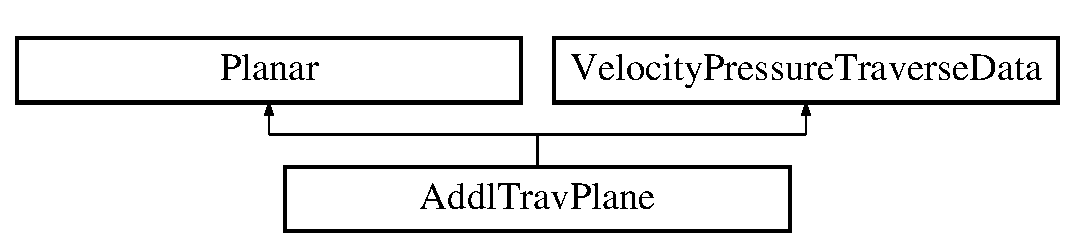
\includegraphics[height=2.000000cm]{d6/dc1/class_addl_trav_plane}
\end{center}
\end{figure}
\subsection*{Public Member Functions}
\begin{DoxyCompactItemize}
\item 
\mbox{\Hypertarget{class_addl_trav_plane_a99ca98acd04b32ad5c949948e0e27cdb}\label{class_addl_trav_plane_a99ca98acd04b32ad5c949948e0e27cdb}} 
{\bfseries Addl\+Trav\+Plane} (double circular\+Duct\+Diameter, double tdx, double pbx, double psx, Tube\+Type tube\+Type, double pitot\+Tube\+Coefficient, std\+::vector$<$ std\+::vector$<$ double $>$ $>$ \&traverse\+Hole\+Data)
\item 
\mbox{\Hypertarget{class_addl_trav_plane_a5d47927388be5a31103f4b7ace4fab37}\label{class_addl_trav_plane_a5d47927388be5a31103f4b7ace4fab37}} 
{\bfseries Addl\+Trav\+Plane} (double rect\+Length, double rect\+Width, double tdx, double pbx, double psx, Tube\+Type tube\+Type, double pitot\+Tube\+Coefficient, std\+::vector$<$ std\+::vector$<$ double $>$ $>$ \&traverse\+Hole\+Data)
\item 
\mbox{\Hypertarget{class_addl_trav_plane_a11033027d926df2358c4f24fe0e85abd}\label{class_addl_trav_plane_a11033027d926df2358c4f24fe0e85abd}} 
{\bfseries Addl\+Trav\+Plane} (double rect\+Length, double rect\+Width, unsigned no\+Inlet\+Boxes, double tdx, double pbx, double psx, Tube\+Type tube\+Type, double pitot\+Tube\+Coefficient, std\+::vector$<$ std\+::vector$<$ double $>$ $>$ \&traverse\+Hole\+Data)
\end{DoxyCompactItemize}
\subsection*{Additional Inherited Members}


\subsection{Detailed Description}


Definition at line 85 of file Planar.\+h.



The documentation for this class was generated from the following files\+:\begin{DoxyCompactItemize}
\item 
include/fans/Planar.\+h\item 
src/fans/Planar.\+cpp\end{DoxyCompactItemize}

\hypertarget{class_compressor_1_1_air_system_capacity}{}\section{Compressor\+:\+:Air\+System\+Capacity Class Reference}
\label{class_compressor_1_1_air_system_capacity}\index{Compressor\+::\+Air\+System\+Capacity@{Compressor\+::\+Air\+System\+Capacity}}
\subsection*{Classes}
\begin{DoxyCompactItemize}
\item 
struct \hyperlink{struct_compressor_1_1_air_system_capacity_1_1_output}{Output}
\end{DoxyCompactItemize}
\subsection*{Public Member Functions}
\begin{DoxyCompactItemize}
\item 
\hyperlink{class_compressor_1_1_air_system_capacity_a270fa85146172b46703970a1bc8fe724}{Air\+System\+Capacity} (\hyperlink{struct_compressor_1_1_pipe_data}{Pipe\+Data} pipe\+Lengths, std\+::vector$<$ double $>$ gallons)
\item 
\mbox{\Hypertarget{class_compressor_1_1_air_system_capacity_aed64b8bb2bfe66e7e8c9df69f5ad3f7e}\label{class_compressor_1_1_air_system_capacity_aed64b8bb2bfe66e7e8c9df69f5ad3f7e}} 
\hyperlink{struct_compressor_1_1_air_system_capacity_1_1_output}{Output} {\bfseries calculate} ()
\end{DoxyCompactItemize}


\subsection{Detailed Description}


Definition at line 237 of file Compressed\+Air.\+h.



\subsection{Constructor \& Destructor Documentation}
\mbox{\Hypertarget{class_compressor_1_1_air_system_capacity_a270fa85146172b46703970a1bc8fe724}\label{class_compressor_1_1_air_system_capacity_a270fa85146172b46703970a1bc8fe724}} 
\index{Compressor\+::\+Air\+System\+Capacity@{Compressor\+::\+Air\+System\+Capacity}!Air\+System\+Capacity@{Air\+System\+Capacity}}
\index{Air\+System\+Capacity@{Air\+System\+Capacity}!Compressor\+::\+Air\+System\+Capacity@{Compressor\+::\+Air\+System\+Capacity}}
\subsubsection{\texorpdfstring{Air\+System\+Capacity()}{AirSystemCapacity()}}
{\footnotesize\ttfamily Compressor\+::\+Air\+System\+Capacity\+::\+Air\+System\+Capacity (\begin{DoxyParamCaption}\item[{\hyperlink{struct_compressor_1_1_pipe_data}{Compressor\+::\+Pipe\+Data}}]{pipe\+Lengths,  }\item[{std\+::vector$<$ double $>$}]{gallons }\end{DoxyParamCaption})}

Constructor for \hyperlink{class_compressor_1_1_air_system_capacity}{Compressor\+::\+Air\+System\+Capacity} -\/ This is used to find the total air quantity that the compressed air system can contain at any instant of time, including the air in the pipes and receivers. 
\begin{DoxyParams}{Parameters}
{\em pipe\+Lengths} & Compressor\+::\+Air\+System\+Capacity\+::\+Pipe\+Lengths, Object containing the lengths of the various pipe sizes in your system -\/ ft \\
\hline
{\em gallons} & std\+::vector$<$double$>$, a vector containing the number of gallons in each receiver \\
\hline
\end{DoxyParams}


Definition at line 103 of file Compressed\+Air.\+cpp.



The documentation for this class was generated from the following files\+:\begin{DoxyCompactItemize}
\item 
include/calculator/util/Compressed\+Air.\+h\item 
src/calculator/util/Compressed\+Air.\+cpp\end{DoxyCompactItemize}

\hypertarget{class_compressor_1_1_air_velocity}{}\section{Compressor\+:\+:Air\+Velocity Class Reference}
\label{class_compressor_1_1_air_velocity}\index{Compressor\+::\+Air\+Velocity@{Compressor\+::\+Air\+Velocity}}
\subsection*{Public Member Functions}
\begin{DoxyCompactItemize}
\item 
\hyperlink{class_compressor_1_1_air_velocity_a53449e5354b1e33db644078ce4d92e4b}{Air\+Velocity} (double air\+Flow, double pipe\+Pressure, double atmospheric\+Pressure)
\item 
\mbox{\Hypertarget{class_compressor_1_1_air_velocity_af17f62700c50a692b4a0db98a11c880c}\label{class_compressor_1_1_air_velocity_af17f62700c50a692b4a0db98a11c880c}} 
\hyperlink{struct_compressor_1_1_pipe_data}{Compressor\+::\+Pipe\+Data} {\bfseries calculate} ()
\item 
\hyperlink{class_compressor_1_1_air_velocity_a53449e5354b1e33db644078ce4d92e4b}{Air\+Velocity} (double air\+Flow, double pipe\+Pressure, double atmospheric\+Pressure)
\item 
\mbox{\Hypertarget{class_compressor_1_1_air_velocity_af17f62700c50a692b4a0db98a11c880c}\label{class_compressor_1_1_air_velocity_af17f62700c50a692b4a0db98a11c880c}} 
\hyperlink{struct_compressor_1_1_pipe_data}{Compressor\+::\+Pipe\+Data} {\bfseries calculate} ()
\item 
\hyperlink{class_compressor_1_1_air_velocity_a53449e5354b1e33db644078ce4d92e4b}{Air\+Velocity} (double air\+Flow, double pipe\+Pressure, double atmospheric\+Pressure)
\item 
\mbox{\Hypertarget{class_compressor_1_1_air_velocity_af17f62700c50a692b4a0db98a11c880c}\label{class_compressor_1_1_air_velocity_af17f62700c50a692b4a0db98a11c880c}} 
\hyperlink{struct_compressor_1_1_pipe_data}{Compressor\+::\+Pipe\+Data} {\bfseries calculate} ()
\end{DoxyCompactItemize}


\subsection{Detailed Description}


Definition at line 268 of file Compressed\+Air.\+h.



\subsection{Constructor \& Destructor Documentation}
\mbox{\Hypertarget{class_compressor_1_1_air_velocity_a53449e5354b1e33db644078ce4d92e4b}\label{class_compressor_1_1_air_velocity_a53449e5354b1e33db644078ce4d92e4b}} 
\index{Compressor\+::\+Air\+Velocity@{Compressor\+::\+Air\+Velocity}!Air\+Velocity@{Air\+Velocity}}
\index{Air\+Velocity@{Air\+Velocity}!Compressor\+::\+Air\+Velocity@{Compressor\+::\+Air\+Velocity}}
\subsubsection{\texorpdfstring{Air\+Velocity()}{AirVelocity()}\hspace{0.1cm}{\footnotesize\ttfamily [1/3]}}
{\footnotesize\ttfamily Compressor\+::\+Air\+Velocity\+::\+Air\+Velocity (\begin{DoxyParamCaption}\item[{double}]{air\+Flow,  }\item[{double}]{pipe\+Pressure,  }\item[{double}]{atmospheric\+Pressure }\end{DoxyParamCaption})}

Constructor for \hyperlink{class_compressor_1_1_air_velocity}{Compressor\+::\+Air\+Velocity} -\/ This calculator finds the velocity of compressed air through all the different piping involved in the system. \begin{DoxyAttention}{Attention}
Constraints -\/ For main and branch lines, recommended maximum velocity is 20 fps, and it should not exceed 30fps. For line drops, feed lines or branch lines, the recommended velocity is 30 fps with an upper limit of 50 fps. 
\end{DoxyAttention}

\begin{DoxyParams}{Parameters}
{\em air\+Flow} & double, Volumetric flow rate of air in the compressor system, referenced to the compressor inlet conditions -\/ scfm \\
\hline
{\em pipe\+Pressure} & double, Pressure of air flowing through the pipe -\/ psig \\
\hline
{\em atmospheric\+Pressure} & double, Generally it will be 14.\+7 -\/ psia \\
\hline
\end{DoxyParams}


Definition at line 120 of file Compressed\+Air.\+cpp.

\mbox{\Hypertarget{class_compressor_1_1_air_velocity_a53449e5354b1e33db644078ce4d92e4b}\label{class_compressor_1_1_air_velocity_a53449e5354b1e33db644078ce4d92e4b}} 
\index{Compressor\+::\+Air\+Velocity@{Compressor\+::\+Air\+Velocity}!Air\+Velocity@{Air\+Velocity}}
\index{Air\+Velocity@{Air\+Velocity}!Compressor\+::\+Air\+Velocity@{Compressor\+::\+Air\+Velocity}}
\subsubsection{\texorpdfstring{Air\+Velocity()}{AirVelocity()}\hspace{0.1cm}{\footnotesize\ttfamily [2/3]}}
{\footnotesize\ttfamily Compressor\+::\+Air\+Velocity\+::\+Air\+Velocity (\begin{DoxyParamCaption}\item[{double}]{air\+Flow,  }\item[{double}]{pipe\+Pressure,  }\item[{double}]{atmospheric\+Pressure }\end{DoxyParamCaption})}

Constructor for \hyperlink{class_compressor_1_1_air_velocity}{Compressor\+::\+Air\+Velocity} -\/ This calculator finds the velocity of compressed air through all the different piping involved in the system. \begin{DoxyAttention}{Attention}
Constraints -\/ For main and branch lines, recommended maximum velocity is 20 fps, and it should not exceed 30fps. For line drops, feed lines or branch lines, the recommended velocity is 30 fps with an upper limit of 50 fps. 
\end{DoxyAttention}

\begin{DoxyParams}{Parameters}
{\em air\+Flow} & double, Volumetric flow rate of air in the compressor system, referenced to the compressor inlet conditions -\/ scfm \\
\hline
{\em pipe\+Pressure} & double, Pressure of air flowing through the pipe -\/ psig \\
\hline
{\em atmospheric\+Pressure} & double, Generally it will be 14.\+7 -\/ psia \\
\hline
\end{DoxyParams}
\mbox{\Hypertarget{class_compressor_1_1_air_velocity_a53449e5354b1e33db644078ce4d92e4b}\label{class_compressor_1_1_air_velocity_a53449e5354b1e33db644078ce4d92e4b}} 
\index{Compressor\+::\+Air\+Velocity@{Compressor\+::\+Air\+Velocity}!Air\+Velocity@{Air\+Velocity}}
\index{Air\+Velocity@{Air\+Velocity}!Compressor\+::\+Air\+Velocity@{Compressor\+::\+Air\+Velocity}}
\subsubsection{\texorpdfstring{Air\+Velocity()}{AirVelocity()}\hspace{0.1cm}{\footnotesize\ttfamily [3/3]}}
{\footnotesize\ttfamily Compressor\+::\+Air\+Velocity\+::\+Air\+Velocity (\begin{DoxyParamCaption}\item[{double}]{air\+Flow,  }\item[{double}]{pipe\+Pressure,  }\item[{double}]{atmospheric\+Pressure }\end{DoxyParamCaption})}

Constructor for \hyperlink{class_compressor_1_1_air_velocity}{Compressor\+::\+Air\+Velocity} -\/ This calculator finds the velocity of compressed air through all the different piping involved in the system. \begin{DoxyAttention}{Attention}
Constraints -\/ For main and branch lines, recommended maximum velocity is 20 fps, and it should not exceed 30fps. For line drops, feed lines or branch lines, the recommended velocity is 30 fps with an upper limit of 50 fps. 
\end{DoxyAttention}

\begin{DoxyParams}{Parameters}
{\em air\+Flow} & double, Volumetric flow rate of air in the compressor system, referenced to the compressor inlet conditions -\/ scfm \\
\hline
{\em pipe\+Pressure} & double, Pressure of air flowing through the pipe -\/ psig \\
\hline
{\em atmospheric\+Pressure} & double, Generally it will be 14.\+7 -\/ psia \\
\hline
\end{DoxyParams}


The documentation for this class was generated from the following files\+:\begin{DoxyCompactItemize}
\item 
\+\_\+\+C\+Pack\+\_\+\+Packages/\+Darwin/\+S\+T\+G\+Z/amo\+\_\+tools\+\_\+suite-\/-\/\+Darwin-\/x86\+\_\+64/amo\+\_\+tools\+\_\+suite/include/calculator/util/Compressed\+Air.\+h\item 
src/calculator/util/Compressed\+Air.\+cpp\end{DoxyCompactItemize}

\hypertarget{class_annual_cost}{}\section{Annual\+Cost Class Reference}
\label{class_annual_cost}\index{Annual\+Cost@{Annual\+Cost}}


\hyperlink{class_header}{Header} file for \hyperlink{class_annual_cost}{Annual\+Cost} class.  




{\ttfamily \#include $<$Annual\+Cost.\+h$>$}

\subsection*{Public Member Functions}
\begin{DoxyCompactItemize}
\item 
\hyperlink{class_annual_cost_a723513a7074d1799e2bf410b60b3146f}{Annual\+Cost} (double annual\+Energy, double kwh\+Rate)
\item 
double \hyperlink{class_annual_cost_adb12b66af50d01746c3f6f0d430b1fdd}{calculate} ()
\begin{DoxyCompactList}\small\item\em Contains the definition of functions of \hyperlink{class_annual_cost}{Annual\+Cost} class. \hyperlink{class_annual_cost_adb12b66af50d01746c3f6f0d430b1fdd}{calculate()}\+: Calculates the annual energy cost. \end{DoxyCompactList}\item 
double \hyperlink{class_annual_cost_a0e217b7df05e6a03503e14d96570a192}{get\+Annual\+Energy} () const
\item 
void \hyperlink{class_annual_cost_a4379cc7b591abefb2302d74c57227357}{set\+Annual\+Energy} (double annual\+Energy)
\item 
double \hyperlink{class_annual_cost_ac01ed415360b6f52f61ec8a581333c29}{get\+Kwh\+Rate} () const
\item 
void \hyperlink{class_annual_cost_a45a1259c9912c7202dff446c290210e9}{set\+Kwh\+Rate} (double kwh\+Rate)
\end{DoxyCompactItemize}


\subsection{Detailed Description}
\hyperlink{class_header}{Header} file for \hyperlink{class_annual_cost}{Annual\+Cost} class. 

This contains the prototypes of \hyperlink{class_annual_cost}{Annual\+Cost} calculator including getters and setters for the important fields.

\begin{DoxyAuthor}{Author}
Subhankar Mishra (mishras) 

Gina Accawi (accawigk) 
\end{DoxyAuthor}


Definition at line 16 of file Annual\+Cost.\+h.



\subsection{Constructor \& Destructor Documentation}
\mbox{\Hypertarget{class_annual_cost_a723513a7074d1799e2bf410b60b3146f}\label{class_annual_cost_a723513a7074d1799e2bf410b60b3146f}} 
\index{Annual\+Cost@{Annual\+Cost}!Annual\+Cost@{Annual\+Cost}}
\index{Annual\+Cost@{Annual\+Cost}!Annual\+Cost@{Annual\+Cost}}
\subsubsection{\texorpdfstring{Annual\+Cost()}{AnnualCost()}}
{\footnotesize\ttfamily Annual\+Cost\+::\+Annual\+Cost (\begin{DoxyParamCaption}\item[{double}]{annual\+Energy,  }\item[{double}]{kwh\+Rate }\end{DoxyParamCaption})\hspace{0.3cm}{\ttfamily [inline]}}

Constructor 
\begin{DoxyParams}{Parameters}
{\em annual\+Energy} & double, annual energy consumption in M\+Wh/year \\
\hline
{\em kwh\+Rate} & double, rate in \$/k\+Wh \\
\hline
\end{DoxyParams}


Definition at line 23 of file Annual\+Cost.\+h.



\subsection{Member Function Documentation}
\mbox{\Hypertarget{class_annual_cost_adb12b66af50d01746c3f6f0d430b1fdd}\label{class_annual_cost_adb12b66af50d01746c3f6f0d430b1fdd}} 
\index{Annual\+Cost@{Annual\+Cost}!calculate@{calculate}}
\index{calculate@{calculate}!Annual\+Cost@{Annual\+Cost}}
\subsubsection{\texorpdfstring{calculate()}{calculate()}}
{\footnotesize\ttfamily double Annual\+Cost\+::calculate (\begin{DoxyParamCaption}{ }\end{DoxyParamCaption})}



Contains the definition of functions of \hyperlink{class_annual_cost}{Annual\+Cost} class. \hyperlink{class_annual_cost_adb12b66af50d01746c3f6f0d430b1fdd}{calculate()}\+: Calculates the annual energy cost. 

Calculates the annual energy cost \begin{DoxyReturn}{Returns}
double, annual energy cost in \$/year
\end{DoxyReturn}
\begin{DoxyAuthor}{Author}
Subhankar Mishra (mishras) 

Gina Accawi (accawigk) 
\end{DoxyAuthor}
Calculate Annual energy cost. Annual energy cost = M\+Wh/year $\ast$ 1000 $\ast$ energy cost rate (\$/k\+Wh) 1000 in above equation is not used in excel version of the tool.

\begin{DoxyReturn}{Returns}
Annual Energy Cost 
\end{DoxyReturn}


Definition at line 20 of file Annual\+Cost.\+cpp.

\mbox{\Hypertarget{class_annual_cost_a0e217b7df05e6a03503e14d96570a192}\label{class_annual_cost_a0e217b7df05e6a03503e14d96570a192}} 
\index{Annual\+Cost@{Annual\+Cost}!get\+Annual\+Energy@{get\+Annual\+Energy}}
\index{get\+Annual\+Energy@{get\+Annual\+Energy}!Annual\+Cost@{Annual\+Cost}}
\subsubsection{\texorpdfstring{get\+Annual\+Energy()}{getAnnualEnergy()}}
{\footnotesize\ttfamily double Annual\+Cost\+::get\+Annual\+Energy (\begin{DoxyParamCaption}{ }\end{DoxyParamCaption}) const\hspace{0.3cm}{\ttfamily [inline]}}

Getter for annual energy. \begin{DoxyReturn}{Returns}
double, annual energy in M\+Wh/year 
\end{DoxyReturn}


Definition at line 41 of file Annual\+Cost.\+h.

\mbox{\Hypertarget{class_annual_cost_ac01ed415360b6f52f61ec8a581333c29}\label{class_annual_cost_ac01ed415360b6f52f61ec8a581333c29}} 
\index{Annual\+Cost@{Annual\+Cost}!get\+Kwh\+Rate@{get\+Kwh\+Rate}}
\index{get\+Kwh\+Rate@{get\+Kwh\+Rate}!Annual\+Cost@{Annual\+Cost}}
\subsubsection{\texorpdfstring{get\+Kwh\+Rate()}{getKwhRate()}}
{\footnotesize\ttfamily double Annual\+Cost\+::get\+Kwh\+Rate (\begin{DoxyParamCaption}{ }\end{DoxyParamCaption}) const\hspace{0.3cm}{\ttfamily [inline]}}

Getter for the rate in \$/k\+Wh \begin{DoxyReturn}{Returns}
double, rate in \$/k\+Wh 
\end{DoxyReturn}


Definition at line 57 of file Annual\+Cost.\+h.

\mbox{\Hypertarget{class_annual_cost_a4379cc7b591abefb2302d74c57227357}\label{class_annual_cost_a4379cc7b591abefb2302d74c57227357}} 
\index{Annual\+Cost@{Annual\+Cost}!set\+Annual\+Energy@{set\+Annual\+Energy}}
\index{set\+Annual\+Energy@{set\+Annual\+Energy}!Annual\+Cost@{Annual\+Cost}}
\subsubsection{\texorpdfstring{set\+Annual\+Energy()}{setAnnualEnergy()}}
{\footnotesize\ttfamily void Annual\+Cost\+::set\+Annual\+Energy (\begin{DoxyParamCaption}\item[{double}]{annual\+Energy }\end{DoxyParamCaption})\hspace{0.3cm}{\ttfamily [inline]}}

Setter for annual energy 
\begin{DoxyParams}{Parameters}
{\em annual\+Energy} & double, annual energy consumption in M\+Wh/year \\
\hline
\end{DoxyParams}


Definition at line 49 of file Annual\+Cost.\+h.

\mbox{\Hypertarget{class_annual_cost_a45a1259c9912c7202dff446c290210e9}\label{class_annual_cost_a45a1259c9912c7202dff446c290210e9}} 
\index{Annual\+Cost@{Annual\+Cost}!set\+Kwh\+Rate@{set\+Kwh\+Rate}}
\index{set\+Kwh\+Rate@{set\+Kwh\+Rate}!Annual\+Cost@{Annual\+Cost}}
\subsubsection{\texorpdfstring{set\+Kwh\+Rate()}{setKwhRate()}}
{\footnotesize\ttfamily void Annual\+Cost\+::set\+Kwh\+Rate (\begin{DoxyParamCaption}\item[{double}]{kwh\+Rate }\end{DoxyParamCaption})\hspace{0.3cm}{\ttfamily [inline]}}

Setter for rate in \$/k\+Wh 
\begin{DoxyParams}{Parameters}
{\em kwh\+Rate} & double, rate in \$/kwh \\
\hline
\end{DoxyParams}


Definition at line 65 of file Annual\+Cost.\+h.



The documentation for this class was generated from the following files\+:\begin{DoxyCompactItemize}
\item 
include/calculator/util/Annual\+Cost.\+h\item 
src/calculator/util/Annual\+Cost.\+cpp\end{DoxyCompactItemize}

\hypertarget{class_annual_energy}{}\section{Annual\+Energy Class Reference}
\label{class_annual_energy}\index{Annual\+Energy@{Annual\+Energy}}


Function prototypes for the Annual Energy.  




{\ttfamily \#include $<$Annual\+Energy.\+h$>$}

\subsection*{Public Member Functions}
\begin{DoxyCompactItemize}
\item 
\hyperlink{class_annual_energy_a5e446ce85879bafeac8fc992cb5b9ed7}{Annual\+Energy} (double field\+Power, double operating\+Fraction)
\item 
double \hyperlink{class_annual_energy_ab599860ffb32ce20a1042a3e9d2ad57f}{calculate} ()
\begin{DoxyCompactList}\small\item\em Contains the definition of functions of \hyperlink{class_annual_energy}{Annual\+Energy} class. \hyperlink{class_annual_energy_ab599860ffb32ce20a1042a3e9d2ad57f}{calculate()}\+: Calculates the annual energy. \end{DoxyCompactList}\item 
double \hyperlink{class_annual_energy_a52aa52274243f578ea7f92d27707cacb}{get\+Field\+Power} () const
\item 
void \hyperlink{class_annual_energy_a4f7212fcf2f6fcd2b12f36ca26a368a1}{set\+Field\+Power} (double field\+Power)
\item 
double \hyperlink{class_annual_energy_a51c2bd68a5268ec9bafe3c70b3a7a6ad}{get\+Operating\+Fraction} () const
\item 
void \hyperlink{class_annual_energy_a5c127c7d5e2a5e4f50559f8b546e8998}{set\+Operating\+Fraction} (double operating\+Fraction)
\end{DoxyCompactItemize}


\subsection{Detailed Description}
Function prototypes for the Annual Energy. 

This contains the prototypes for the Annual Energy calculator including getters and setters for the important fields.

\begin{DoxyAuthor}{Author}
Subhankar Mishra (mishras) 

Gina Accawi (accawigk) 
\end{DoxyAuthor}


Definition at line 16 of file Annual\+Energy.\+h.



\subsection{Constructor \& Destructor Documentation}
\mbox{\Hypertarget{class_annual_energy_a5e446ce85879bafeac8fc992cb5b9ed7}\label{class_annual_energy_a5e446ce85879bafeac8fc992cb5b9ed7}} 
\index{Annual\+Energy@{Annual\+Energy}!Annual\+Energy@{Annual\+Energy}}
\index{Annual\+Energy@{Annual\+Energy}!Annual\+Energy@{Annual\+Energy}}
\subsubsection{\texorpdfstring{Annual\+Energy()}{AnnualEnergy()}}
{\footnotesize\ttfamily Annual\+Energy\+::\+Annual\+Energy (\begin{DoxyParamCaption}\item[{double}]{field\+Power,  }\item[{double}]{operating\+Fraction }\end{DoxyParamCaption})\hspace{0.3cm}{\ttfamily [inline]}}

Constructor 
\begin{DoxyParams}{Parameters}
{\em field\+Power} & double, power from field data in hp \\
\hline
{\em operating\+Fraction} & double, perating fraction(\%). \\
\hline
\end{DoxyParams}


Definition at line 23 of file Annual\+Energy.\+h.



\subsection{Member Function Documentation}
\mbox{\Hypertarget{class_annual_energy_ab599860ffb32ce20a1042a3e9d2ad57f}\label{class_annual_energy_ab599860ffb32ce20a1042a3e9d2ad57f}} 
\index{Annual\+Energy@{Annual\+Energy}!calculate@{calculate}}
\index{calculate@{calculate}!Annual\+Energy@{Annual\+Energy}}
\subsubsection{\texorpdfstring{calculate()}{calculate()}}
{\footnotesize\ttfamily double Annual\+Energy\+::calculate (\begin{DoxyParamCaption}{ }\end{DoxyParamCaption})}



Contains the definition of functions of \hyperlink{class_annual_energy}{Annual\+Energy} class. \hyperlink{class_annual_energy_ab599860ffb32ce20a1042a3e9d2ad57f}{calculate()}\+: Calculates the annual energy. 

Calculates annual energy \begin{DoxyReturn}{Returns}
double, annual energy in M\+Wh/year
\end{DoxyReturn}
\begin{DoxyAuthor}{Author}
Subhankar Mishra (mishras) 

Gina Accawi (accawigk) 
\end{DoxyAuthor}
Calculates annual energy Annual energy, M\+Wh/year = k\+We $\ast$ 8760 hrs/year $\ast$ operating fraction/1000 \begin{DoxyReturn}{Returns}
Annual Energy 
\end{DoxyReturn}


Definition at line 18 of file Annual\+Energy.\+cpp.

\mbox{\Hypertarget{class_annual_energy_a52aa52274243f578ea7f92d27707cacb}\label{class_annual_energy_a52aa52274243f578ea7f92d27707cacb}} 
\index{Annual\+Energy@{Annual\+Energy}!get\+Field\+Power@{get\+Field\+Power}}
\index{get\+Field\+Power@{get\+Field\+Power}!Annual\+Energy@{Annual\+Energy}}
\subsubsection{\texorpdfstring{get\+Field\+Power()}{getFieldPower()}}
{\footnotesize\ttfamily double Annual\+Energy\+::get\+Field\+Power (\begin{DoxyParamCaption}{ }\end{DoxyParamCaption}) const\hspace{0.3cm}{\ttfamily [inline]}}

Getter for field power \begin{DoxyReturn}{Returns}
double, power from field data in hp 
\end{DoxyReturn}


Definition at line 41 of file Annual\+Energy.\+h.

\mbox{\Hypertarget{class_annual_energy_a51c2bd68a5268ec9bafe3c70b3a7a6ad}\label{class_annual_energy_a51c2bd68a5268ec9bafe3c70b3a7a6ad}} 
\index{Annual\+Energy@{Annual\+Energy}!get\+Operating\+Fraction@{get\+Operating\+Fraction}}
\index{get\+Operating\+Fraction@{get\+Operating\+Fraction}!Annual\+Energy@{Annual\+Energy}}
\subsubsection{\texorpdfstring{get\+Operating\+Fraction()}{getOperatingFraction()}}
{\footnotesize\ttfamily double Annual\+Energy\+::get\+Operating\+Fraction (\begin{DoxyParamCaption}{ }\end{DoxyParamCaption}) const\hspace{0.3cm}{\ttfamily [inline]}}

Getter for operating fraction \begin{DoxyReturn}{Returns}
double, operating fraction as \% 
\end{DoxyReturn}


Definition at line 57 of file Annual\+Energy.\+h.

\mbox{\Hypertarget{class_annual_energy_a4f7212fcf2f6fcd2b12f36ca26a368a1}\label{class_annual_energy_a4f7212fcf2f6fcd2b12f36ca26a368a1}} 
\index{Annual\+Energy@{Annual\+Energy}!set\+Field\+Power@{set\+Field\+Power}}
\index{set\+Field\+Power@{set\+Field\+Power}!Annual\+Energy@{Annual\+Energy}}
\subsubsection{\texorpdfstring{set\+Field\+Power()}{setFieldPower()}}
{\footnotesize\ttfamily void Annual\+Energy\+::set\+Field\+Power (\begin{DoxyParamCaption}\item[{double}]{field\+Power }\end{DoxyParamCaption})\hspace{0.3cm}{\ttfamily [inline]}}

Setter for field power 
\begin{DoxyParams}{Parameters}
{\em field\+Power} & double, power from field data in hp \\
\hline
\end{DoxyParams}


Definition at line 49 of file Annual\+Energy.\+h.

\mbox{\Hypertarget{class_annual_energy_a5c127c7d5e2a5e4f50559f8b546e8998}\label{class_annual_energy_a5c127c7d5e2a5e4f50559f8b546e8998}} 
\index{Annual\+Energy@{Annual\+Energy}!set\+Operating\+Fraction@{set\+Operating\+Fraction}}
\index{set\+Operating\+Fraction@{set\+Operating\+Fraction}!Annual\+Energy@{Annual\+Energy}}
\subsubsection{\texorpdfstring{set\+Operating\+Fraction()}{setOperatingFraction()}}
{\footnotesize\ttfamily void Annual\+Energy\+::set\+Operating\+Fraction (\begin{DoxyParamCaption}\item[{double}]{operating\+Fraction }\end{DoxyParamCaption})\hspace{0.3cm}{\ttfamily [inline]}}

Setter for operating fraction


\begin{DoxyParams}{Parameters}
{\em operating\+Fraction} & double, operating fraction as \% \\
\hline
\end{DoxyParams}


Definition at line 67 of file Annual\+Energy.\+h.



The documentation for this class was generated from the following files\+:\begin{DoxyCompactItemize}
\item 
include/calculator/util/Annual\+Energy.\+h\item 
src/calculator/util/Annual\+Energy.\+cpp\end{DoxyCompactItemize}

\hypertarget{class_atmosphere}{}\section{Atmosphere Class Reference}
\label{class_atmosphere}\index{Atmosphere@{Atmosphere}}


{\ttfamily \#include $<$Atmosphere.\+h$>$}

\subsection*{Public Member Functions}
\begin{DoxyCompactItemize}
\item 
\hyperlink{class_atmosphere_adbd727cfc7682d3b3b72a4fb101531f1}{Atmosphere} (const double inlet\+Temperature, const double outlet\+Temperature, const double flow\+Rate, const double correction\+Factor, const double specific\+Heat)
\item 
double \hyperlink{class_atmosphere_acb944a3a99cd40f0132713ce73e6ca4a}{get\+Inlet\+Temperature} () const
\item 
void \hyperlink{class_atmosphere_a592bf7f82ea518fbd9da86d8f10cbc5c}{set\+Inlet\+Temperature} (const double inlet\+Temperature)
\item 
double \hyperlink{class_atmosphere_a717e2dc78ebd13420f8f26707374dd3f}{get\+Outlet\+Temperature} () const
\item 
void \hyperlink{class_atmosphere_a8f6589ab4e17d3c531bb7e0e771f4f80}{set\+Outlet\+Temperature} (const double outlet\+Temperature)
\item 
double \hyperlink{class_atmosphere_ad34708b12c8c9af4fce47669d68ebf4d}{get\+Flow\+Rate} () const
\item 
void \hyperlink{class_atmosphere_a9ff0b718c810aec0bb101336db69fd22}{set\+Flow\+Rate} (const double flow\+Rate)
\item 
double \hyperlink{class_atmosphere_a79c94343c7b6659b2f79688a1ba69aed}{get\+Correction\+Factor} () const
\item 
void \hyperlink{class_atmosphere_a86fab4b05de35c9a2b1a3a7e5ab70779}{set\+Correction\+Factor} (const double correction\+Factor)
\item 
double \hyperlink{class_atmosphere_a59802a10861a58ab0f0f4e0ab8671e14}{get\+Specific\+Heat} () const
\item 
void \hyperlink{class_atmosphere_a17450de3bc7a64b2736b1fe8785410cd}{set\+Specific\+Heat} (const double specific\+Heat)
\item 
double \hyperlink{class_atmosphere_ad3dd28020262aee76d374cbfb7998e46}{get\+Total\+Heat} ()
\item 
std\+::string \hyperlink{class_atmosphere_a3ac0fb0d4fc92edc690e44b40b7018c2}{get\+Substance} () const
\item 
void \hyperlink{class_atmosphere_aa92f55a1f07304f3e57fdfb8ece65d82}{set\+Substance} (std\+::string substance)
\item 
int \hyperlink{class_atmosphere_a73b921f4d29a4a409488cbdb56c53ff7}{get\+ID} () const
\item 
void \hyperlink{class_atmosphere_a4698bf2580f7c24c8e0617d6455bfcac}{set\+ID} (const int id)
\item 
\mbox{\Hypertarget{class_atmosphere_a6bddf411a91af4808f52cd69033a5c54}\label{class_atmosphere_a6bddf411a91af4808f52cd69033a5c54}} 
bool \hyperlink{class_atmosphere_a6bddf411a91af4808f52cd69033a5c54}{operator==} (const \hyperlink{class_atmosphere}{Atmosphere} \&rhs) const
\begin{DoxyCompactList}\small\item\em bool operator \end{DoxyCompactList}\item 
\mbox{\Hypertarget{class_atmosphere_a8f75154e49eb74561dc9053607f502f9}\label{class_atmosphere_a8f75154e49eb74561dc9053607f502f9}} 
bool \hyperlink{class_atmosphere_a8f75154e49eb74561dc9053607f502f9}{operator!=} (const \hyperlink{class_atmosphere}{Atmosphere} \&rhs) const
\begin{DoxyCompactList}\small\item\em bool operator \end{DoxyCompactList}\item 
\hyperlink{class_atmosphere_adbd727cfc7682d3b3b72a4fb101531f1}{Atmosphere} (const double inlet\+Temperature, const double outlet\+Temperature, const double flow\+Rate, const double correction\+Factor, const double specific\+Heat)
\item 
double \hyperlink{class_atmosphere_acb944a3a99cd40f0132713ce73e6ca4a}{get\+Inlet\+Temperature} () const
\item 
void \hyperlink{class_atmosphere_a592bf7f82ea518fbd9da86d8f10cbc5c}{set\+Inlet\+Temperature} (const double inlet\+Temperature)
\item 
double \hyperlink{class_atmosphere_a717e2dc78ebd13420f8f26707374dd3f}{get\+Outlet\+Temperature} () const
\item 
void \hyperlink{class_atmosphere_a8f6589ab4e17d3c531bb7e0e771f4f80}{set\+Outlet\+Temperature} (const double outlet\+Temperature)
\item 
double \hyperlink{class_atmosphere_ad34708b12c8c9af4fce47669d68ebf4d}{get\+Flow\+Rate} () const
\item 
void \hyperlink{class_atmosphere_a9ff0b718c810aec0bb101336db69fd22}{set\+Flow\+Rate} (const double flow\+Rate)
\item 
double \hyperlink{class_atmosphere_a79c94343c7b6659b2f79688a1ba69aed}{get\+Correction\+Factor} () const
\item 
void \hyperlink{class_atmosphere_a86fab4b05de35c9a2b1a3a7e5ab70779}{set\+Correction\+Factor} (const double correction\+Factor)
\item 
double \hyperlink{class_atmosphere_a59802a10861a58ab0f0f4e0ab8671e14}{get\+Specific\+Heat} () const
\item 
void \hyperlink{class_atmosphere_a17450de3bc7a64b2736b1fe8785410cd}{set\+Specific\+Heat} (const double specific\+Heat)
\item 
double \hyperlink{class_atmosphere_ad3dd28020262aee76d374cbfb7998e46}{get\+Total\+Heat} ()
\item 
std\+::string \hyperlink{class_atmosphere_a3ac0fb0d4fc92edc690e44b40b7018c2}{get\+Substance} () const
\item 
void \hyperlink{class_atmosphere_aa92f55a1f07304f3e57fdfb8ece65d82}{set\+Substance} (std\+::string substance)
\item 
int \hyperlink{class_atmosphere_a73b921f4d29a4a409488cbdb56c53ff7}{get\+ID} () const
\item 
void \hyperlink{class_atmosphere_a4698bf2580f7c24c8e0617d6455bfcac}{set\+ID} (const int id)
\item 
\mbox{\Hypertarget{class_atmosphere_a6bddf411a91af4808f52cd69033a5c54}\label{class_atmosphere_a6bddf411a91af4808f52cd69033a5c54}} 
bool \hyperlink{class_atmosphere_a6bddf411a91af4808f52cd69033a5c54}{operator==} (const \hyperlink{class_atmosphere}{Atmosphere} \&rhs) const
\begin{DoxyCompactList}\small\item\em bool operator \end{DoxyCompactList}\item 
\mbox{\Hypertarget{class_atmosphere_a8f75154e49eb74561dc9053607f502f9}\label{class_atmosphere_a8f75154e49eb74561dc9053607f502f9}} 
bool \hyperlink{class_atmosphere_a8f75154e49eb74561dc9053607f502f9}{operator!=} (const \hyperlink{class_atmosphere}{Atmosphere} \&rhs) const
\begin{DoxyCompactList}\small\item\em bool operator \end{DoxyCompactList}\item 
\hyperlink{class_atmosphere_adbd727cfc7682d3b3b72a4fb101531f1}{Atmosphere} (const double inlet\+Temperature, const double outlet\+Temperature, const double flow\+Rate, const double correction\+Factor, const double specific\+Heat)
\item 
double \hyperlink{class_atmosphere_acb944a3a99cd40f0132713ce73e6ca4a}{get\+Inlet\+Temperature} () const
\item 
void \hyperlink{class_atmosphere_a592bf7f82ea518fbd9da86d8f10cbc5c}{set\+Inlet\+Temperature} (const double inlet\+Temperature)
\item 
double \hyperlink{class_atmosphere_a717e2dc78ebd13420f8f26707374dd3f}{get\+Outlet\+Temperature} () const
\item 
void \hyperlink{class_atmosphere_a8f6589ab4e17d3c531bb7e0e771f4f80}{set\+Outlet\+Temperature} (const double outlet\+Temperature)
\item 
double \hyperlink{class_atmosphere_ad34708b12c8c9af4fce47669d68ebf4d}{get\+Flow\+Rate} () const
\item 
void \hyperlink{class_atmosphere_a9ff0b718c810aec0bb101336db69fd22}{set\+Flow\+Rate} (const double flow\+Rate)
\item 
double \hyperlink{class_atmosphere_a79c94343c7b6659b2f79688a1ba69aed}{get\+Correction\+Factor} () const
\item 
void \hyperlink{class_atmosphere_a86fab4b05de35c9a2b1a3a7e5ab70779}{set\+Correction\+Factor} (const double correction\+Factor)
\item 
double \hyperlink{class_atmosphere_a59802a10861a58ab0f0f4e0ab8671e14}{get\+Specific\+Heat} () const
\item 
void \hyperlink{class_atmosphere_a17450de3bc7a64b2736b1fe8785410cd}{set\+Specific\+Heat} (const double specific\+Heat)
\item 
double \hyperlink{class_atmosphere_ad3dd28020262aee76d374cbfb7998e46}{get\+Total\+Heat} ()
\item 
std\+::string \hyperlink{class_atmosphere_a3ac0fb0d4fc92edc690e44b40b7018c2}{get\+Substance} () const
\item 
void \hyperlink{class_atmosphere_aa92f55a1f07304f3e57fdfb8ece65d82}{set\+Substance} (std\+::string substance)
\item 
int \hyperlink{class_atmosphere_a73b921f4d29a4a409488cbdb56c53ff7}{get\+ID} () const
\item 
void \hyperlink{class_atmosphere_a4698bf2580f7c24c8e0617d6455bfcac}{set\+ID} (const int id)
\item 
\mbox{\Hypertarget{class_atmosphere_a6bddf411a91af4808f52cd69033a5c54}\label{class_atmosphere_a6bddf411a91af4808f52cd69033a5c54}} 
bool \hyperlink{class_atmosphere_a6bddf411a91af4808f52cd69033a5c54}{operator==} (const \hyperlink{class_atmosphere}{Atmosphere} \&rhs) const
\begin{DoxyCompactList}\small\item\em bool operator \end{DoxyCompactList}\item 
\mbox{\Hypertarget{class_atmosphere_a8f75154e49eb74561dc9053607f502f9}\label{class_atmosphere_a8f75154e49eb74561dc9053607f502f9}} 
bool \hyperlink{class_atmosphere_a8f75154e49eb74561dc9053607f502f9}{operator!=} (const \hyperlink{class_atmosphere}{Atmosphere} \&rhs) const
\begin{DoxyCompactList}\small\item\em bool operator \end{DoxyCompactList}\end{DoxyCompactItemize}
\subsection*{Friends}
\begin{DoxyCompactItemize}
\item 
\mbox{\Hypertarget{class_atmosphere_a0102f3b3c0cbf96db6c49f071fa5e7cc}\label{class_atmosphere_a0102f3b3c0cbf96db6c49f071fa5e7cc}} 
class {\bfseries S\+Q\+Lite}
\end{DoxyCompactItemize}


\subsection{Detailed Description}
\hyperlink{class_atmosphere}{Atmosphere} class Contains all of the properties of the atmosphere of gases within the furnace. Used to calculate how much heat is used by the atmosphere gases. A\+S\+S\+U\+M\+P\+T\+I\+O\+NS\+: The atmosphere composition does not change. There is not heat of reaction (endothermic or exothermic) between the atmosphere and materials inside the furnace. W\+A\+R\+N\+I\+N\+GS\+: If the atmosphere reacts with the material being processed, then its composition changes, and it is necessary to use appropriate correction factors based on new and old composition properties. 

Definition at line 31 of file Atmosphere.\+h.



\subsection{Constructor \& Destructor Documentation}
\mbox{\Hypertarget{class_atmosphere_adbd727cfc7682d3b3b72a4fb101531f1}\label{class_atmosphere_adbd727cfc7682d3b3b72a4fb101531f1}} 
\index{Atmosphere@{Atmosphere}!Atmosphere@{Atmosphere}}
\index{Atmosphere@{Atmosphere}!Atmosphere@{Atmosphere}}
\subsubsection{\texorpdfstring{Atmosphere()}{Atmosphere()}\hspace{0.1cm}{\footnotesize\ttfamily [1/3]}}
{\footnotesize\ttfamily Atmosphere\+::\+Atmosphere (\begin{DoxyParamCaption}\item[{const double}]{inlet\+Temperature,  }\item[{const double}]{outlet\+Temperature,  }\item[{const double}]{flow\+Rate,  }\item[{const double}]{correction\+Factor,  }\item[{const double}]{specific\+Heat }\end{DoxyParamCaption})\hspace{0.3cm}{\ttfamily [inline]}}

Constructor for the atmospheric heat loss with all inputs specified


\begin{DoxyParams}{Parameters}
{\em inlet\+Temperature} & double, inlet temperature of gasses in °F \\
\hline
{\em outlet\+Temperature} & double, outlet temperature of gasses in °F \\
\hline
{\em flow\+Rate} & double, flow rate of gasses in scfh \\
\hline
{\em correction\+Factor} & double, correction factor -\/ unitless \\
\hline
{\em specific\+Heat} & double, specific heat of gasses at average air temperature in Btu/(scf$\ast$°F) \\
\hline
\end{DoxyParams}


Definition at line 45 of file Atmosphere.\+h.

\mbox{\Hypertarget{class_atmosphere_adbd727cfc7682d3b3b72a4fb101531f1}\label{class_atmosphere_adbd727cfc7682d3b3b72a4fb101531f1}} 
\index{Atmosphere@{Atmosphere}!Atmosphere@{Atmosphere}}
\index{Atmosphere@{Atmosphere}!Atmosphere@{Atmosphere}}
\subsubsection{\texorpdfstring{Atmosphere()}{Atmosphere()}\hspace{0.1cm}{\footnotesize\ttfamily [2/3]}}
{\footnotesize\ttfamily Atmosphere\+::\+Atmosphere (\begin{DoxyParamCaption}\item[{const double}]{inlet\+Temperature,  }\item[{const double}]{outlet\+Temperature,  }\item[{const double}]{flow\+Rate,  }\item[{const double}]{correction\+Factor,  }\item[{const double}]{specific\+Heat }\end{DoxyParamCaption})\hspace{0.3cm}{\ttfamily [inline]}}

Constructor for the atmospheric heat loss with all inputs specified


\begin{DoxyParams}{Parameters}
{\em inlet\+Temperature} & double, inlet temperature of gasses in °F \\
\hline
{\em outlet\+Temperature} & double, outlet temperature of gasses in °F \\
\hline
{\em flow\+Rate} & double, flow rate of gasses in scfh \\
\hline
{\em correction\+Factor} & double, correction factor -\/ unitless \\
\hline
{\em specific\+Heat} & double, specific heat of gasses at average air temperature in Btu/(scf$\ast$°F) \\
\hline
\end{DoxyParams}


Definition at line 45 of file Atmosphere.\+h.

\mbox{\Hypertarget{class_atmosphere_adbd727cfc7682d3b3b72a4fb101531f1}\label{class_atmosphere_adbd727cfc7682d3b3b72a4fb101531f1}} 
\index{Atmosphere@{Atmosphere}!Atmosphere@{Atmosphere}}
\index{Atmosphere@{Atmosphere}!Atmosphere@{Atmosphere}}
\subsubsection{\texorpdfstring{Atmosphere()}{Atmosphere()}\hspace{0.1cm}{\footnotesize\ttfamily [3/3]}}
{\footnotesize\ttfamily Atmosphere\+::\+Atmosphere (\begin{DoxyParamCaption}\item[{const double}]{inlet\+Temperature,  }\item[{const double}]{outlet\+Temperature,  }\item[{const double}]{flow\+Rate,  }\item[{const double}]{correction\+Factor,  }\item[{const double}]{specific\+Heat }\end{DoxyParamCaption})\hspace{0.3cm}{\ttfamily [inline]}}

Constructor for the atmospheric heat loss with all inputs specified


\begin{DoxyParams}{Parameters}
{\em inlet\+Temperature} & double, inlet temperature of gasses in °F \\
\hline
{\em outlet\+Temperature} & double, outlet temperature of gasses in °F \\
\hline
{\em flow\+Rate} & double, flow rate of gasses in scfh \\
\hline
{\em correction\+Factor} & double, correction factor -\/ unitless \\
\hline
{\em specific\+Heat} & double, specific heat of gasses at average air temperature in Btu/(scf$\ast$°F) \\
\hline
\end{DoxyParams}


Definition at line 45 of file Atmosphere.\+h.



\subsection{Member Function Documentation}
\mbox{\Hypertarget{class_atmosphere_a79c94343c7b6659b2f79688a1ba69aed}\label{class_atmosphere_a79c94343c7b6659b2f79688a1ba69aed}} 
\index{Atmosphere@{Atmosphere}!get\+Correction\+Factor@{get\+Correction\+Factor}}
\index{get\+Correction\+Factor@{get\+Correction\+Factor}!Atmosphere@{Atmosphere}}
\subsubsection{\texorpdfstring{get\+Correction\+Factor()}{getCorrectionFactor()}\hspace{0.1cm}{\footnotesize\ttfamily [1/3]}}
{\footnotesize\ttfamily double Atmosphere\+::get\+Correction\+Factor (\begin{DoxyParamCaption}{ }\end{DoxyParamCaption}) const\hspace{0.3cm}{\ttfamily [inline]}}

Getter for the correction factor \begin{DoxyReturn}{Returns}
double, correction factor -\/ unitless 
\end{DoxyReturn}


Definition at line 110 of file Atmosphere.\+h.

\mbox{\Hypertarget{class_atmosphere_a79c94343c7b6659b2f79688a1ba69aed}\label{class_atmosphere_a79c94343c7b6659b2f79688a1ba69aed}} 
\index{Atmosphere@{Atmosphere}!get\+Correction\+Factor@{get\+Correction\+Factor}}
\index{get\+Correction\+Factor@{get\+Correction\+Factor}!Atmosphere@{Atmosphere}}
\subsubsection{\texorpdfstring{get\+Correction\+Factor()}{getCorrectionFactor()}\hspace{0.1cm}{\footnotesize\ttfamily [2/3]}}
{\footnotesize\ttfamily double Atmosphere\+::get\+Correction\+Factor (\begin{DoxyParamCaption}{ }\end{DoxyParamCaption}) const\hspace{0.3cm}{\ttfamily [inline]}}

Getter for the correction factor \begin{DoxyReturn}{Returns}
double, correction factor -\/ unitless 
\end{DoxyReturn}


Definition at line 110 of file Atmosphere.\+h.

\mbox{\Hypertarget{class_atmosphere_a79c94343c7b6659b2f79688a1ba69aed}\label{class_atmosphere_a79c94343c7b6659b2f79688a1ba69aed}} 
\index{Atmosphere@{Atmosphere}!get\+Correction\+Factor@{get\+Correction\+Factor}}
\index{get\+Correction\+Factor@{get\+Correction\+Factor}!Atmosphere@{Atmosphere}}
\subsubsection{\texorpdfstring{get\+Correction\+Factor()}{getCorrectionFactor()}\hspace{0.1cm}{\footnotesize\ttfamily [3/3]}}
{\footnotesize\ttfamily double Atmosphere\+::get\+Correction\+Factor (\begin{DoxyParamCaption}{ }\end{DoxyParamCaption}) const\hspace{0.3cm}{\ttfamily [inline]}}

Getter for the correction factor \begin{DoxyReturn}{Returns}
double, correction factor -\/ unitless 
\end{DoxyReturn}


Definition at line 110 of file Atmosphere.\+h.

\mbox{\Hypertarget{class_atmosphere_ad34708b12c8c9af4fce47669d68ebf4d}\label{class_atmosphere_ad34708b12c8c9af4fce47669d68ebf4d}} 
\index{Atmosphere@{Atmosphere}!get\+Flow\+Rate@{get\+Flow\+Rate}}
\index{get\+Flow\+Rate@{get\+Flow\+Rate}!Atmosphere@{Atmosphere}}
\subsubsection{\texorpdfstring{get\+Flow\+Rate()}{getFlowRate()}\hspace{0.1cm}{\footnotesize\ttfamily [1/3]}}
{\footnotesize\ttfamily double Atmosphere\+::get\+Flow\+Rate (\begin{DoxyParamCaption}{ }\end{DoxyParamCaption}) const\hspace{0.3cm}{\ttfamily [inline]}}

Getter for the flow rate \begin{DoxyReturn}{Returns}
double, flow rate in scfh 
\end{DoxyReturn}


Definition at line 94 of file Atmosphere.\+h.

\mbox{\Hypertarget{class_atmosphere_ad34708b12c8c9af4fce47669d68ebf4d}\label{class_atmosphere_ad34708b12c8c9af4fce47669d68ebf4d}} 
\index{Atmosphere@{Atmosphere}!get\+Flow\+Rate@{get\+Flow\+Rate}}
\index{get\+Flow\+Rate@{get\+Flow\+Rate}!Atmosphere@{Atmosphere}}
\subsubsection{\texorpdfstring{get\+Flow\+Rate()}{getFlowRate()}\hspace{0.1cm}{\footnotesize\ttfamily [2/3]}}
{\footnotesize\ttfamily double Atmosphere\+::get\+Flow\+Rate (\begin{DoxyParamCaption}{ }\end{DoxyParamCaption}) const\hspace{0.3cm}{\ttfamily [inline]}}

Getter for the flow rate \begin{DoxyReturn}{Returns}
double, flow rate in scfh 
\end{DoxyReturn}


Definition at line 94 of file Atmosphere.\+h.

\mbox{\Hypertarget{class_atmosphere_ad34708b12c8c9af4fce47669d68ebf4d}\label{class_atmosphere_ad34708b12c8c9af4fce47669d68ebf4d}} 
\index{Atmosphere@{Atmosphere}!get\+Flow\+Rate@{get\+Flow\+Rate}}
\index{get\+Flow\+Rate@{get\+Flow\+Rate}!Atmosphere@{Atmosphere}}
\subsubsection{\texorpdfstring{get\+Flow\+Rate()}{getFlowRate()}\hspace{0.1cm}{\footnotesize\ttfamily [3/3]}}
{\footnotesize\ttfamily double Atmosphere\+::get\+Flow\+Rate (\begin{DoxyParamCaption}{ }\end{DoxyParamCaption}) const\hspace{0.3cm}{\ttfamily [inline]}}

Getter for the flow rate \begin{DoxyReturn}{Returns}
double, flow rate in scfh 
\end{DoxyReturn}


Definition at line 94 of file Atmosphere.\+h.

\mbox{\Hypertarget{class_atmosphere_a73b921f4d29a4a409488cbdb56c53ff7}\label{class_atmosphere_a73b921f4d29a4a409488cbdb56c53ff7}} 
\index{Atmosphere@{Atmosphere}!get\+ID@{get\+ID}}
\index{get\+ID@{get\+ID}!Atmosphere@{Atmosphere}}
\subsubsection{\texorpdfstring{get\+I\+D()}{getID()}\hspace{0.1cm}{\footnotesize\ttfamily [1/3]}}
{\footnotesize\ttfamily int Atmosphere\+::get\+ID (\begin{DoxyParamCaption}{ }\end{DoxyParamCaption}) const\hspace{0.3cm}{\ttfamily [inline]}}

Gets the ID of material \begin{DoxyReturn}{Returns}
int, ID of material 
\end{DoxyReturn}


Definition at line 164 of file Atmosphere.\+h.

\mbox{\Hypertarget{class_atmosphere_a73b921f4d29a4a409488cbdb56c53ff7}\label{class_atmosphere_a73b921f4d29a4a409488cbdb56c53ff7}} 
\index{Atmosphere@{Atmosphere}!get\+ID@{get\+ID}}
\index{get\+ID@{get\+ID}!Atmosphere@{Atmosphere}}
\subsubsection{\texorpdfstring{get\+I\+D()}{getID()}\hspace{0.1cm}{\footnotesize\ttfamily [2/3]}}
{\footnotesize\ttfamily int Atmosphere\+::get\+ID (\begin{DoxyParamCaption}{ }\end{DoxyParamCaption}) const\hspace{0.3cm}{\ttfamily [inline]}}

Gets the ID of material \begin{DoxyReturn}{Returns}
int, ID of material 
\end{DoxyReturn}


Definition at line 164 of file Atmosphere.\+h.

\mbox{\Hypertarget{class_atmosphere_a73b921f4d29a4a409488cbdb56c53ff7}\label{class_atmosphere_a73b921f4d29a4a409488cbdb56c53ff7}} 
\index{Atmosphere@{Atmosphere}!get\+ID@{get\+ID}}
\index{get\+ID@{get\+ID}!Atmosphere@{Atmosphere}}
\subsubsection{\texorpdfstring{get\+I\+D()}{getID()}\hspace{0.1cm}{\footnotesize\ttfamily [3/3]}}
{\footnotesize\ttfamily int Atmosphere\+::get\+ID (\begin{DoxyParamCaption}{ }\end{DoxyParamCaption}) const\hspace{0.3cm}{\ttfamily [inline]}}

Gets the ID of material \begin{DoxyReturn}{Returns}
int, ID of material 
\end{DoxyReturn}


Definition at line 164 of file Atmosphere.\+h.

\mbox{\Hypertarget{class_atmosphere_acb944a3a99cd40f0132713ce73e6ca4a}\label{class_atmosphere_acb944a3a99cd40f0132713ce73e6ca4a}} 
\index{Atmosphere@{Atmosphere}!get\+Inlet\+Temperature@{get\+Inlet\+Temperature}}
\index{get\+Inlet\+Temperature@{get\+Inlet\+Temperature}!Atmosphere@{Atmosphere}}
\subsubsection{\texorpdfstring{get\+Inlet\+Temperature()}{getInletTemperature()}\hspace{0.1cm}{\footnotesize\ttfamily [1/3]}}
{\footnotesize\ttfamily double Atmosphere\+::get\+Inlet\+Temperature (\begin{DoxyParamCaption}{ }\end{DoxyParamCaption}) const\hspace{0.3cm}{\ttfamily [inline]}}

Getter for the inlet/initial temperature \begin{DoxyReturn}{Returns}
double, inlet/initial temperature in °F 
\end{DoxyReturn}


Definition at line 62 of file Atmosphere.\+h.

\mbox{\Hypertarget{class_atmosphere_acb944a3a99cd40f0132713ce73e6ca4a}\label{class_atmosphere_acb944a3a99cd40f0132713ce73e6ca4a}} 
\index{Atmosphere@{Atmosphere}!get\+Inlet\+Temperature@{get\+Inlet\+Temperature}}
\index{get\+Inlet\+Temperature@{get\+Inlet\+Temperature}!Atmosphere@{Atmosphere}}
\subsubsection{\texorpdfstring{get\+Inlet\+Temperature()}{getInletTemperature()}\hspace{0.1cm}{\footnotesize\ttfamily [2/3]}}
{\footnotesize\ttfamily double Atmosphere\+::get\+Inlet\+Temperature (\begin{DoxyParamCaption}{ }\end{DoxyParamCaption}) const\hspace{0.3cm}{\ttfamily [inline]}}

Getter for the inlet/initial temperature \begin{DoxyReturn}{Returns}
double, inlet/initial temperature in °F 
\end{DoxyReturn}


Definition at line 62 of file Atmosphere.\+h.

\mbox{\Hypertarget{class_atmosphere_acb944a3a99cd40f0132713ce73e6ca4a}\label{class_atmosphere_acb944a3a99cd40f0132713ce73e6ca4a}} 
\index{Atmosphere@{Atmosphere}!get\+Inlet\+Temperature@{get\+Inlet\+Temperature}}
\index{get\+Inlet\+Temperature@{get\+Inlet\+Temperature}!Atmosphere@{Atmosphere}}
\subsubsection{\texorpdfstring{get\+Inlet\+Temperature()}{getInletTemperature()}\hspace{0.1cm}{\footnotesize\ttfamily [3/3]}}
{\footnotesize\ttfamily double Atmosphere\+::get\+Inlet\+Temperature (\begin{DoxyParamCaption}{ }\end{DoxyParamCaption}) const\hspace{0.3cm}{\ttfamily [inline]}}

Getter for the inlet/initial temperature \begin{DoxyReturn}{Returns}
double, inlet/initial temperature in °F 
\end{DoxyReturn}


Definition at line 62 of file Atmosphere.\+h.

\mbox{\Hypertarget{class_atmosphere_a717e2dc78ebd13420f8f26707374dd3f}\label{class_atmosphere_a717e2dc78ebd13420f8f26707374dd3f}} 
\index{Atmosphere@{Atmosphere}!get\+Outlet\+Temperature@{get\+Outlet\+Temperature}}
\index{get\+Outlet\+Temperature@{get\+Outlet\+Temperature}!Atmosphere@{Atmosphere}}
\subsubsection{\texorpdfstring{get\+Outlet\+Temperature()}{getOutletTemperature()}\hspace{0.1cm}{\footnotesize\ttfamily [1/3]}}
{\footnotesize\ttfamily double Atmosphere\+::get\+Outlet\+Temperature (\begin{DoxyParamCaption}{ }\end{DoxyParamCaption}) const\hspace{0.3cm}{\ttfamily [inline]}}

Getter for the outlet/final temperature \begin{DoxyReturn}{Returns}
double, outlet/final temperature in °F 
\end{DoxyReturn}


Definition at line 78 of file Atmosphere.\+h.

\mbox{\Hypertarget{class_atmosphere_a717e2dc78ebd13420f8f26707374dd3f}\label{class_atmosphere_a717e2dc78ebd13420f8f26707374dd3f}} 
\index{Atmosphere@{Atmosphere}!get\+Outlet\+Temperature@{get\+Outlet\+Temperature}}
\index{get\+Outlet\+Temperature@{get\+Outlet\+Temperature}!Atmosphere@{Atmosphere}}
\subsubsection{\texorpdfstring{get\+Outlet\+Temperature()}{getOutletTemperature()}\hspace{0.1cm}{\footnotesize\ttfamily [2/3]}}
{\footnotesize\ttfamily double Atmosphere\+::get\+Outlet\+Temperature (\begin{DoxyParamCaption}{ }\end{DoxyParamCaption}) const\hspace{0.3cm}{\ttfamily [inline]}}

Getter for the outlet/final temperature \begin{DoxyReturn}{Returns}
double, outlet/final temperature in °F 
\end{DoxyReturn}


Definition at line 78 of file Atmosphere.\+h.

\mbox{\Hypertarget{class_atmosphere_a717e2dc78ebd13420f8f26707374dd3f}\label{class_atmosphere_a717e2dc78ebd13420f8f26707374dd3f}} 
\index{Atmosphere@{Atmosphere}!get\+Outlet\+Temperature@{get\+Outlet\+Temperature}}
\index{get\+Outlet\+Temperature@{get\+Outlet\+Temperature}!Atmosphere@{Atmosphere}}
\subsubsection{\texorpdfstring{get\+Outlet\+Temperature()}{getOutletTemperature()}\hspace{0.1cm}{\footnotesize\ttfamily [3/3]}}
{\footnotesize\ttfamily double Atmosphere\+::get\+Outlet\+Temperature (\begin{DoxyParamCaption}{ }\end{DoxyParamCaption}) const\hspace{0.3cm}{\ttfamily [inline]}}

Getter for the outlet/final temperature \begin{DoxyReturn}{Returns}
double, outlet/final temperature in °F 
\end{DoxyReturn}


Definition at line 78 of file Atmosphere.\+h.

\mbox{\Hypertarget{class_atmosphere_a59802a10861a58ab0f0f4e0ab8671e14}\label{class_atmosphere_a59802a10861a58ab0f0f4e0ab8671e14}} 
\index{Atmosphere@{Atmosphere}!get\+Specific\+Heat@{get\+Specific\+Heat}}
\index{get\+Specific\+Heat@{get\+Specific\+Heat}!Atmosphere@{Atmosphere}}
\subsubsection{\texorpdfstring{get\+Specific\+Heat()}{getSpecificHeat()}\hspace{0.1cm}{\footnotesize\ttfamily [1/3]}}
{\footnotesize\ttfamily double Atmosphere\+::get\+Specific\+Heat (\begin{DoxyParamCaption}{ }\end{DoxyParamCaption}) const\hspace{0.3cm}{\ttfamily [inline]}}

Getter for the specific heat \begin{DoxyReturn}{Returns}
double, specific heat in btu/(scf$\ast$°F) 
\end{DoxyReturn}


Definition at line 126 of file Atmosphere.\+h.

\mbox{\Hypertarget{class_atmosphere_a59802a10861a58ab0f0f4e0ab8671e14}\label{class_atmosphere_a59802a10861a58ab0f0f4e0ab8671e14}} 
\index{Atmosphere@{Atmosphere}!get\+Specific\+Heat@{get\+Specific\+Heat}}
\index{get\+Specific\+Heat@{get\+Specific\+Heat}!Atmosphere@{Atmosphere}}
\subsubsection{\texorpdfstring{get\+Specific\+Heat()}{getSpecificHeat()}\hspace{0.1cm}{\footnotesize\ttfamily [2/3]}}
{\footnotesize\ttfamily double Atmosphere\+::get\+Specific\+Heat (\begin{DoxyParamCaption}{ }\end{DoxyParamCaption}) const\hspace{0.3cm}{\ttfamily [inline]}}

Getter for the specific heat \begin{DoxyReturn}{Returns}
double, specific heat in btu/(scf$\ast$°F) 
\end{DoxyReturn}


Definition at line 126 of file Atmosphere.\+h.

\mbox{\Hypertarget{class_atmosphere_a59802a10861a58ab0f0f4e0ab8671e14}\label{class_atmosphere_a59802a10861a58ab0f0f4e0ab8671e14}} 
\index{Atmosphere@{Atmosphere}!get\+Specific\+Heat@{get\+Specific\+Heat}}
\index{get\+Specific\+Heat@{get\+Specific\+Heat}!Atmosphere@{Atmosphere}}
\subsubsection{\texorpdfstring{get\+Specific\+Heat()}{getSpecificHeat()}\hspace{0.1cm}{\footnotesize\ttfamily [3/3]}}
{\footnotesize\ttfamily double Atmosphere\+::get\+Specific\+Heat (\begin{DoxyParamCaption}{ }\end{DoxyParamCaption}) const\hspace{0.3cm}{\ttfamily [inline]}}

Getter for the specific heat \begin{DoxyReturn}{Returns}
double, specific heat in btu/(scf$\ast$°F) 
\end{DoxyReturn}


Definition at line 126 of file Atmosphere.\+h.

\mbox{\Hypertarget{class_atmosphere_a3ac0fb0d4fc92edc690e44b40b7018c2}\label{class_atmosphere_a3ac0fb0d4fc92edc690e44b40b7018c2}} 
\index{Atmosphere@{Atmosphere}!get\+Substance@{get\+Substance}}
\index{get\+Substance@{get\+Substance}!Atmosphere@{Atmosphere}}
\subsubsection{\texorpdfstring{get\+Substance()}{getSubstance()}\hspace{0.1cm}{\footnotesize\ttfamily [1/3]}}
{\footnotesize\ttfamily std\+::string Atmosphere\+::get\+Substance (\begin{DoxyParamCaption}{ }\end{DoxyParamCaption}) const\hspace{0.3cm}{\ttfamily [inline]}}

Gets the name of substance \begin{DoxyReturn}{Returns}
string, name of substance 
\end{DoxyReturn}


Definition at line 148 of file Atmosphere.\+h.

\mbox{\Hypertarget{class_atmosphere_a3ac0fb0d4fc92edc690e44b40b7018c2}\label{class_atmosphere_a3ac0fb0d4fc92edc690e44b40b7018c2}} 
\index{Atmosphere@{Atmosphere}!get\+Substance@{get\+Substance}}
\index{get\+Substance@{get\+Substance}!Atmosphere@{Atmosphere}}
\subsubsection{\texorpdfstring{get\+Substance()}{getSubstance()}\hspace{0.1cm}{\footnotesize\ttfamily [2/3]}}
{\footnotesize\ttfamily std\+::string Atmosphere\+::get\+Substance (\begin{DoxyParamCaption}{ }\end{DoxyParamCaption}) const\hspace{0.3cm}{\ttfamily [inline]}}

Gets the name of substance \begin{DoxyReturn}{Returns}
string, name of substance 
\end{DoxyReturn}


Definition at line 148 of file Atmosphere.\+h.

\mbox{\Hypertarget{class_atmosphere_a3ac0fb0d4fc92edc690e44b40b7018c2}\label{class_atmosphere_a3ac0fb0d4fc92edc690e44b40b7018c2}} 
\index{Atmosphere@{Atmosphere}!get\+Substance@{get\+Substance}}
\index{get\+Substance@{get\+Substance}!Atmosphere@{Atmosphere}}
\subsubsection{\texorpdfstring{get\+Substance()}{getSubstance()}\hspace{0.1cm}{\footnotesize\ttfamily [3/3]}}
{\footnotesize\ttfamily std\+::string Atmosphere\+::get\+Substance (\begin{DoxyParamCaption}{ }\end{DoxyParamCaption}) const\hspace{0.3cm}{\ttfamily [inline]}}

Gets the name of substance \begin{DoxyReturn}{Returns}
string, name of substance 
\end{DoxyReturn}


Definition at line 148 of file Atmosphere.\+h.

\mbox{\Hypertarget{class_atmosphere_ad3dd28020262aee76d374cbfb7998e46}\label{class_atmosphere_ad3dd28020262aee76d374cbfb7998e46}} 
\index{Atmosphere@{Atmosphere}!get\+Total\+Heat@{get\+Total\+Heat}}
\index{get\+Total\+Heat@{get\+Total\+Heat}!Atmosphere@{Atmosphere}}
\subsubsection{\texorpdfstring{get\+Total\+Heat()}{getTotalHeat()}\hspace{0.1cm}{\footnotesize\ttfamily [1/3]}}
{\footnotesize\ttfamily double Atmosphere\+::get\+Total\+Heat (\begin{DoxyParamCaption}{ }\end{DoxyParamCaption})}

Calculates the total heat loss \begin{DoxyReturn}{Returns}
double, total heat loss in btu/hr 
\end{DoxyReturn}


Definition at line 11 of file Atmosphere.\+cpp.

\mbox{\Hypertarget{class_atmosphere_ad3dd28020262aee76d374cbfb7998e46}\label{class_atmosphere_ad3dd28020262aee76d374cbfb7998e46}} 
\index{Atmosphere@{Atmosphere}!get\+Total\+Heat@{get\+Total\+Heat}}
\index{get\+Total\+Heat@{get\+Total\+Heat}!Atmosphere@{Atmosphere}}
\subsubsection{\texorpdfstring{get\+Total\+Heat()}{getTotalHeat()}\hspace{0.1cm}{\footnotesize\ttfamily [2/3]}}
{\footnotesize\ttfamily double Atmosphere\+::get\+Total\+Heat (\begin{DoxyParamCaption}{ }\end{DoxyParamCaption})}

Calculates the total heat loss \begin{DoxyReturn}{Returns}
double, total heat loss in btu/hr 
\end{DoxyReturn}
\mbox{\Hypertarget{class_atmosphere_ad3dd28020262aee76d374cbfb7998e46}\label{class_atmosphere_ad3dd28020262aee76d374cbfb7998e46}} 
\index{Atmosphere@{Atmosphere}!get\+Total\+Heat@{get\+Total\+Heat}}
\index{get\+Total\+Heat@{get\+Total\+Heat}!Atmosphere@{Atmosphere}}
\subsubsection{\texorpdfstring{get\+Total\+Heat()}{getTotalHeat()}\hspace{0.1cm}{\footnotesize\ttfamily [3/3]}}
{\footnotesize\ttfamily double Atmosphere\+::get\+Total\+Heat (\begin{DoxyParamCaption}{ }\end{DoxyParamCaption})}

Calculates the total heat loss \begin{DoxyReturn}{Returns}
double, total heat loss in btu/hr 
\end{DoxyReturn}
\mbox{\Hypertarget{class_atmosphere_a86fab4b05de35c9a2b1a3a7e5ab70779}\label{class_atmosphere_a86fab4b05de35c9a2b1a3a7e5ab70779}} 
\index{Atmosphere@{Atmosphere}!set\+Correction\+Factor@{set\+Correction\+Factor}}
\index{set\+Correction\+Factor@{set\+Correction\+Factor}!Atmosphere@{Atmosphere}}
\subsubsection{\texorpdfstring{set\+Correction\+Factor()}{setCorrectionFactor()}\hspace{0.1cm}{\footnotesize\ttfamily [1/3]}}
{\footnotesize\ttfamily void Atmosphere\+::set\+Correction\+Factor (\begin{DoxyParamCaption}\item[{const double}]{correction\+Factor }\end{DoxyParamCaption})\hspace{0.3cm}{\ttfamily [inline]}}

Sets the correction factor 
\begin{DoxyParams}{Parameters}
{\em correction\+Factor} & double, correction factor -\/ unitless \\
\hline
\end{DoxyParams}


Definition at line 118 of file Atmosphere.\+h.

\mbox{\Hypertarget{class_atmosphere_a86fab4b05de35c9a2b1a3a7e5ab70779}\label{class_atmosphere_a86fab4b05de35c9a2b1a3a7e5ab70779}} 
\index{Atmosphere@{Atmosphere}!set\+Correction\+Factor@{set\+Correction\+Factor}}
\index{set\+Correction\+Factor@{set\+Correction\+Factor}!Atmosphere@{Atmosphere}}
\subsubsection{\texorpdfstring{set\+Correction\+Factor()}{setCorrectionFactor()}\hspace{0.1cm}{\footnotesize\ttfamily [2/3]}}
{\footnotesize\ttfamily void Atmosphere\+::set\+Correction\+Factor (\begin{DoxyParamCaption}\item[{const double}]{correction\+Factor }\end{DoxyParamCaption})\hspace{0.3cm}{\ttfamily [inline]}}

Sets the correction factor 
\begin{DoxyParams}{Parameters}
{\em correction\+Factor} & double, correction factor -\/ unitless \\
\hline
\end{DoxyParams}


Definition at line 118 of file Atmosphere.\+h.

\mbox{\Hypertarget{class_atmosphere_a86fab4b05de35c9a2b1a3a7e5ab70779}\label{class_atmosphere_a86fab4b05de35c9a2b1a3a7e5ab70779}} 
\index{Atmosphere@{Atmosphere}!set\+Correction\+Factor@{set\+Correction\+Factor}}
\index{set\+Correction\+Factor@{set\+Correction\+Factor}!Atmosphere@{Atmosphere}}
\subsubsection{\texorpdfstring{set\+Correction\+Factor()}{setCorrectionFactor()}\hspace{0.1cm}{\footnotesize\ttfamily [3/3]}}
{\footnotesize\ttfamily void Atmosphere\+::set\+Correction\+Factor (\begin{DoxyParamCaption}\item[{const double}]{correction\+Factor }\end{DoxyParamCaption})\hspace{0.3cm}{\ttfamily [inline]}}

Sets the correction factor 
\begin{DoxyParams}{Parameters}
{\em correction\+Factor} & double, correction factor -\/ unitless \\
\hline
\end{DoxyParams}


Definition at line 118 of file Atmosphere.\+h.

\mbox{\Hypertarget{class_atmosphere_a9ff0b718c810aec0bb101336db69fd22}\label{class_atmosphere_a9ff0b718c810aec0bb101336db69fd22}} 
\index{Atmosphere@{Atmosphere}!set\+Flow\+Rate@{set\+Flow\+Rate}}
\index{set\+Flow\+Rate@{set\+Flow\+Rate}!Atmosphere@{Atmosphere}}
\subsubsection{\texorpdfstring{set\+Flow\+Rate()}{setFlowRate()}\hspace{0.1cm}{\footnotesize\ttfamily [1/3]}}
{\footnotesize\ttfamily void Atmosphere\+::set\+Flow\+Rate (\begin{DoxyParamCaption}\item[{const double}]{flow\+Rate }\end{DoxyParamCaption})\hspace{0.3cm}{\ttfamily [inline]}}

Sets the flow rate 
\begin{DoxyParams}{Parameters}
{\em flow\+Rate} & double, flow rate in scfh \\
\hline
\end{DoxyParams}


Definition at line 102 of file Atmosphere.\+h.

\mbox{\Hypertarget{class_atmosphere_a9ff0b718c810aec0bb101336db69fd22}\label{class_atmosphere_a9ff0b718c810aec0bb101336db69fd22}} 
\index{Atmosphere@{Atmosphere}!set\+Flow\+Rate@{set\+Flow\+Rate}}
\index{set\+Flow\+Rate@{set\+Flow\+Rate}!Atmosphere@{Atmosphere}}
\subsubsection{\texorpdfstring{set\+Flow\+Rate()}{setFlowRate()}\hspace{0.1cm}{\footnotesize\ttfamily [2/3]}}
{\footnotesize\ttfamily void Atmosphere\+::set\+Flow\+Rate (\begin{DoxyParamCaption}\item[{const double}]{flow\+Rate }\end{DoxyParamCaption})\hspace{0.3cm}{\ttfamily [inline]}}

Sets the flow rate 
\begin{DoxyParams}{Parameters}
{\em flow\+Rate} & double, flow rate in scfh \\
\hline
\end{DoxyParams}


Definition at line 102 of file Atmosphere.\+h.

\mbox{\Hypertarget{class_atmosphere_a9ff0b718c810aec0bb101336db69fd22}\label{class_atmosphere_a9ff0b718c810aec0bb101336db69fd22}} 
\index{Atmosphere@{Atmosphere}!set\+Flow\+Rate@{set\+Flow\+Rate}}
\index{set\+Flow\+Rate@{set\+Flow\+Rate}!Atmosphere@{Atmosphere}}
\subsubsection{\texorpdfstring{set\+Flow\+Rate()}{setFlowRate()}\hspace{0.1cm}{\footnotesize\ttfamily [3/3]}}
{\footnotesize\ttfamily void Atmosphere\+::set\+Flow\+Rate (\begin{DoxyParamCaption}\item[{const double}]{flow\+Rate }\end{DoxyParamCaption})\hspace{0.3cm}{\ttfamily [inline]}}

Sets the flow rate 
\begin{DoxyParams}{Parameters}
{\em flow\+Rate} & double, flow rate in scfh \\
\hline
\end{DoxyParams}


Definition at line 102 of file Atmosphere.\+h.

\mbox{\Hypertarget{class_atmosphere_a4698bf2580f7c24c8e0617d6455bfcac}\label{class_atmosphere_a4698bf2580f7c24c8e0617d6455bfcac}} 
\index{Atmosphere@{Atmosphere}!set\+ID@{set\+ID}}
\index{set\+ID@{set\+ID}!Atmosphere@{Atmosphere}}
\subsubsection{\texorpdfstring{set\+I\+D()}{setID()}\hspace{0.1cm}{\footnotesize\ttfamily [1/3]}}
{\footnotesize\ttfamily void Atmosphere\+::set\+ID (\begin{DoxyParamCaption}\item[{const int}]{id }\end{DoxyParamCaption})\hspace{0.3cm}{\ttfamily [inline]}}

Sets the ID of material 
\begin{DoxyParams}{Parameters}
{\em id} & const int, ID of material \\
\hline
\end{DoxyParams}


Definition at line 172 of file Atmosphere.\+h.

\mbox{\Hypertarget{class_atmosphere_a4698bf2580f7c24c8e0617d6455bfcac}\label{class_atmosphere_a4698bf2580f7c24c8e0617d6455bfcac}} 
\index{Atmosphere@{Atmosphere}!set\+ID@{set\+ID}}
\index{set\+ID@{set\+ID}!Atmosphere@{Atmosphere}}
\subsubsection{\texorpdfstring{set\+I\+D()}{setID()}\hspace{0.1cm}{\footnotesize\ttfamily [2/3]}}
{\footnotesize\ttfamily void Atmosphere\+::set\+ID (\begin{DoxyParamCaption}\item[{const int}]{id }\end{DoxyParamCaption})\hspace{0.3cm}{\ttfamily [inline]}}

Sets the ID of material 
\begin{DoxyParams}{Parameters}
{\em id} & const int, ID of material \\
\hline
\end{DoxyParams}


Definition at line 172 of file Atmosphere.\+h.

\mbox{\Hypertarget{class_atmosphere_a4698bf2580f7c24c8e0617d6455bfcac}\label{class_atmosphere_a4698bf2580f7c24c8e0617d6455bfcac}} 
\index{Atmosphere@{Atmosphere}!set\+ID@{set\+ID}}
\index{set\+ID@{set\+ID}!Atmosphere@{Atmosphere}}
\subsubsection{\texorpdfstring{set\+I\+D()}{setID()}\hspace{0.1cm}{\footnotesize\ttfamily [3/3]}}
{\footnotesize\ttfamily void Atmosphere\+::set\+ID (\begin{DoxyParamCaption}\item[{const int}]{id }\end{DoxyParamCaption})\hspace{0.3cm}{\ttfamily [inline]}}

Sets the ID of material 
\begin{DoxyParams}{Parameters}
{\em id} & const int, ID of material \\
\hline
\end{DoxyParams}


Definition at line 172 of file Atmosphere.\+h.

\mbox{\Hypertarget{class_atmosphere_a592bf7f82ea518fbd9da86d8f10cbc5c}\label{class_atmosphere_a592bf7f82ea518fbd9da86d8f10cbc5c}} 
\index{Atmosphere@{Atmosphere}!set\+Inlet\+Temperature@{set\+Inlet\+Temperature}}
\index{set\+Inlet\+Temperature@{set\+Inlet\+Temperature}!Atmosphere@{Atmosphere}}
\subsubsection{\texorpdfstring{set\+Inlet\+Temperature()}{setInletTemperature()}\hspace{0.1cm}{\footnotesize\ttfamily [1/3]}}
{\footnotesize\ttfamily void Atmosphere\+::set\+Inlet\+Temperature (\begin{DoxyParamCaption}\item[{const double}]{inlet\+Temperature }\end{DoxyParamCaption})\hspace{0.3cm}{\ttfamily [inline]}}

Sets the inlet/initial temperature 
\begin{DoxyParams}{Parameters}
{\em inlet\+Temperature} & double, initial temperature in °F \\
\hline
\end{DoxyParams}


Definition at line 70 of file Atmosphere.\+h.

\mbox{\Hypertarget{class_atmosphere_a592bf7f82ea518fbd9da86d8f10cbc5c}\label{class_atmosphere_a592bf7f82ea518fbd9da86d8f10cbc5c}} 
\index{Atmosphere@{Atmosphere}!set\+Inlet\+Temperature@{set\+Inlet\+Temperature}}
\index{set\+Inlet\+Temperature@{set\+Inlet\+Temperature}!Atmosphere@{Atmosphere}}
\subsubsection{\texorpdfstring{set\+Inlet\+Temperature()}{setInletTemperature()}\hspace{0.1cm}{\footnotesize\ttfamily [2/3]}}
{\footnotesize\ttfamily void Atmosphere\+::set\+Inlet\+Temperature (\begin{DoxyParamCaption}\item[{const double}]{inlet\+Temperature }\end{DoxyParamCaption})\hspace{0.3cm}{\ttfamily [inline]}}

Sets the inlet/initial temperature 
\begin{DoxyParams}{Parameters}
{\em inlet\+Temperature} & double, initial temperature in °F \\
\hline
\end{DoxyParams}


Definition at line 70 of file Atmosphere.\+h.

\mbox{\Hypertarget{class_atmosphere_a592bf7f82ea518fbd9da86d8f10cbc5c}\label{class_atmosphere_a592bf7f82ea518fbd9da86d8f10cbc5c}} 
\index{Atmosphere@{Atmosphere}!set\+Inlet\+Temperature@{set\+Inlet\+Temperature}}
\index{set\+Inlet\+Temperature@{set\+Inlet\+Temperature}!Atmosphere@{Atmosphere}}
\subsubsection{\texorpdfstring{set\+Inlet\+Temperature()}{setInletTemperature()}\hspace{0.1cm}{\footnotesize\ttfamily [3/3]}}
{\footnotesize\ttfamily void Atmosphere\+::set\+Inlet\+Temperature (\begin{DoxyParamCaption}\item[{const double}]{inlet\+Temperature }\end{DoxyParamCaption})\hspace{0.3cm}{\ttfamily [inline]}}

Sets the inlet/initial temperature 
\begin{DoxyParams}{Parameters}
{\em inlet\+Temperature} & double, initial temperature in °F \\
\hline
\end{DoxyParams}


Definition at line 70 of file Atmosphere.\+h.

\mbox{\Hypertarget{class_atmosphere_a8f6589ab4e17d3c531bb7e0e771f4f80}\label{class_atmosphere_a8f6589ab4e17d3c531bb7e0e771f4f80}} 
\index{Atmosphere@{Atmosphere}!set\+Outlet\+Temperature@{set\+Outlet\+Temperature}}
\index{set\+Outlet\+Temperature@{set\+Outlet\+Temperature}!Atmosphere@{Atmosphere}}
\subsubsection{\texorpdfstring{set\+Outlet\+Temperature()}{setOutletTemperature()}\hspace{0.1cm}{\footnotesize\ttfamily [1/3]}}
{\footnotesize\ttfamily void Atmosphere\+::set\+Outlet\+Temperature (\begin{DoxyParamCaption}\item[{const double}]{outlet\+Temperature }\end{DoxyParamCaption})\hspace{0.3cm}{\ttfamily [inline]}}

Sets the outlet/final temperature 
\begin{DoxyParams}{Parameters}
{\em outlet\+Temperature} & double, outlet/final temperature in °F \\
\hline
\end{DoxyParams}


Definition at line 86 of file Atmosphere.\+h.

\mbox{\Hypertarget{class_atmosphere_a8f6589ab4e17d3c531bb7e0e771f4f80}\label{class_atmosphere_a8f6589ab4e17d3c531bb7e0e771f4f80}} 
\index{Atmosphere@{Atmosphere}!set\+Outlet\+Temperature@{set\+Outlet\+Temperature}}
\index{set\+Outlet\+Temperature@{set\+Outlet\+Temperature}!Atmosphere@{Atmosphere}}
\subsubsection{\texorpdfstring{set\+Outlet\+Temperature()}{setOutletTemperature()}\hspace{0.1cm}{\footnotesize\ttfamily [2/3]}}
{\footnotesize\ttfamily void Atmosphere\+::set\+Outlet\+Temperature (\begin{DoxyParamCaption}\item[{const double}]{outlet\+Temperature }\end{DoxyParamCaption})\hspace{0.3cm}{\ttfamily [inline]}}

Sets the outlet/final temperature 
\begin{DoxyParams}{Parameters}
{\em outlet\+Temperature} & double, outlet/final temperature in °F \\
\hline
\end{DoxyParams}


Definition at line 86 of file Atmosphere.\+h.

\mbox{\Hypertarget{class_atmosphere_a8f6589ab4e17d3c531bb7e0e771f4f80}\label{class_atmosphere_a8f6589ab4e17d3c531bb7e0e771f4f80}} 
\index{Atmosphere@{Atmosphere}!set\+Outlet\+Temperature@{set\+Outlet\+Temperature}}
\index{set\+Outlet\+Temperature@{set\+Outlet\+Temperature}!Atmosphere@{Atmosphere}}
\subsubsection{\texorpdfstring{set\+Outlet\+Temperature()}{setOutletTemperature()}\hspace{0.1cm}{\footnotesize\ttfamily [3/3]}}
{\footnotesize\ttfamily void Atmosphere\+::set\+Outlet\+Temperature (\begin{DoxyParamCaption}\item[{const double}]{outlet\+Temperature }\end{DoxyParamCaption})\hspace{0.3cm}{\ttfamily [inline]}}

Sets the outlet/final temperature 
\begin{DoxyParams}{Parameters}
{\em outlet\+Temperature} & double, outlet/final temperature in °F \\
\hline
\end{DoxyParams}


Definition at line 86 of file Atmosphere.\+h.

\mbox{\Hypertarget{class_atmosphere_a17450de3bc7a64b2736b1fe8785410cd}\label{class_atmosphere_a17450de3bc7a64b2736b1fe8785410cd}} 
\index{Atmosphere@{Atmosphere}!set\+Specific\+Heat@{set\+Specific\+Heat}}
\index{set\+Specific\+Heat@{set\+Specific\+Heat}!Atmosphere@{Atmosphere}}
\subsubsection{\texorpdfstring{set\+Specific\+Heat()}{setSpecificHeat()}\hspace{0.1cm}{\footnotesize\ttfamily [1/3]}}
{\footnotesize\ttfamily void Atmosphere\+::set\+Specific\+Heat (\begin{DoxyParamCaption}\item[{const double}]{specific\+Heat }\end{DoxyParamCaption})\hspace{0.3cm}{\ttfamily [inline]}}

Sets the specific heat 
\begin{DoxyParams}{Parameters}
{\em specific\+Heat} & double, specific heat in btu/(scf$\ast$°F) \\
\hline
\end{DoxyParams}


Definition at line 134 of file Atmosphere.\+h.

\mbox{\Hypertarget{class_atmosphere_a17450de3bc7a64b2736b1fe8785410cd}\label{class_atmosphere_a17450de3bc7a64b2736b1fe8785410cd}} 
\index{Atmosphere@{Atmosphere}!set\+Specific\+Heat@{set\+Specific\+Heat}}
\index{set\+Specific\+Heat@{set\+Specific\+Heat}!Atmosphere@{Atmosphere}}
\subsubsection{\texorpdfstring{set\+Specific\+Heat()}{setSpecificHeat()}\hspace{0.1cm}{\footnotesize\ttfamily [2/3]}}
{\footnotesize\ttfamily void Atmosphere\+::set\+Specific\+Heat (\begin{DoxyParamCaption}\item[{const double}]{specific\+Heat }\end{DoxyParamCaption})\hspace{0.3cm}{\ttfamily [inline]}}

Sets the specific heat 
\begin{DoxyParams}{Parameters}
{\em specific\+Heat} & double, specific heat in btu/(scf$\ast$°F) \\
\hline
\end{DoxyParams}


Definition at line 134 of file Atmosphere.\+h.

\mbox{\Hypertarget{class_atmosphere_a17450de3bc7a64b2736b1fe8785410cd}\label{class_atmosphere_a17450de3bc7a64b2736b1fe8785410cd}} 
\index{Atmosphere@{Atmosphere}!set\+Specific\+Heat@{set\+Specific\+Heat}}
\index{set\+Specific\+Heat@{set\+Specific\+Heat}!Atmosphere@{Atmosphere}}
\subsubsection{\texorpdfstring{set\+Specific\+Heat()}{setSpecificHeat()}\hspace{0.1cm}{\footnotesize\ttfamily [3/3]}}
{\footnotesize\ttfamily void Atmosphere\+::set\+Specific\+Heat (\begin{DoxyParamCaption}\item[{const double}]{specific\+Heat }\end{DoxyParamCaption})\hspace{0.3cm}{\ttfamily [inline]}}

Sets the specific heat 
\begin{DoxyParams}{Parameters}
{\em specific\+Heat} & double, specific heat in btu/(scf$\ast$°F) \\
\hline
\end{DoxyParams}


Definition at line 134 of file Atmosphere.\+h.

\mbox{\Hypertarget{class_atmosphere_aa92f55a1f07304f3e57fdfb8ece65d82}\label{class_atmosphere_aa92f55a1f07304f3e57fdfb8ece65d82}} 
\index{Atmosphere@{Atmosphere}!set\+Substance@{set\+Substance}}
\index{set\+Substance@{set\+Substance}!Atmosphere@{Atmosphere}}
\subsubsection{\texorpdfstring{set\+Substance()}{setSubstance()}\hspace{0.1cm}{\footnotesize\ttfamily [1/3]}}
{\footnotesize\ttfamily void Atmosphere\+::set\+Substance (\begin{DoxyParamCaption}\item[{std\+::string}]{substance }\end{DoxyParamCaption})\hspace{0.3cm}{\ttfamily [inline]}}

Sets the name of substance 
\begin{DoxyParams}{Parameters}
{\em substance} & string, name of substance \\
\hline
\end{DoxyParams}


Definition at line 156 of file Atmosphere.\+h.

\mbox{\Hypertarget{class_atmosphere_aa92f55a1f07304f3e57fdfb8ece65d82}\label{class_atmosphere_aa92f55a1f07304f3e57fdfb8ece65d82}} 
\index{Atmosphere@{Atmosphere}!set\+Substance@{set\+Substance}}
\index{set\+Substance@{set\+Substance}!Atmosphere@{Atmosphere}}
\subsubsection{\texorpdfstring{set\+Substance()}{setSubstance()}\hspace{0.1cm}{\footnotesize\ttfamily [2/3]}}
{\footnotesize\ttfamily void Atmosphere\+::set\+Substance (\begin{DoxyParamCaption}\item[{std\+::string}]{substance }\end{DoxyParamCaption})\hspace{0.3cm}{\ttfamily [inline]}}

Sets the name of substance 
\begin{DoxyParams}{Parameters}
{\em substance} & string, name of substance \\
\hline
\end{DoxyParams}


Definition at line 156 of file Atmosphere.\+h.

\mbox{\Hypertarget{class_atmosphere_aa92f55a1f07304f3e57fdfb8ece65d82}\label{class_atmosphere_aa92f55a1f07304f3e57fdfb8ece65d82}} 
\index{Atmosphere@{Atmosphere}!set\+Substance@{set\+Substance}}
\index{set\+Substance@{set\+Substance}!Atmosphere@{Atmosphere}}
\subsubsection{\texorpdfstring{set\+Substance()}{setSubstance()}\hspace{0.1cm}{\footnotesize\ttfamily [3/3]}}
{\footnotesize\ttfamily void Atmosphere\+::set\+Substance (\begin{DoxyParamCaption}\item[{std\+::string}]{substance }\end{DoxyParamCaption})\hspace{0.3cm}{\ttfamily [inline]}}

Sets the name of substance 
\begin{DoxyParams}{Parameters}
{\em substance} & string, name of substance \\
\hline
\end{DoxyParams}


Definition at line 156 of file Atmosphere.\+h.



The documentation for this class was generated from the following files\+:\begin{DoxyCompactItemize}
\item 
\+\_\+\+C\+Pack\+\_\+\+Packages/\+Darwin/\+S\+T\+G\+Z/amo\+\_\+tools\+\_\+suite-\/-\/\+Darwin-\/x86\+\_\+64-\/\+Debug/amo\+\_\+tools\+\_\+suite/include/calculator/losses/\hyperlink{___c_pack___packages_2_darwin_2_s_t_g_z_2amo__tools__suite--_darwin-x86__64-_debug_2amo__tools__7727b2302b92ae6542446d85da658463}{Atmosphere.\+h}\item 
src/calculator/losses/\hyperlink{_atmosphere_8cpp}{Atmosphere.\+cpp}\end{DoxyCompactItemize}

\hypertarget{class_auxiliary_power}{}\section{Auxiliary\+Power Class Reference}
\label{class_auxiliary_power}\index{Auxiliary\+Power@{Auxiliary\+Power}}


{\ttfamily \#include $<$Auxiliary\+Power.\+h$>$}

\subsection*{Public Member Functions}
\begin{DoxyCompactItemize}
\item 
\hyperlink{class_auxiliary_power_aef0d5c2c60a2481b16cc201ba2e69fe7}{Auxiliary\+Power} (const double motor\+Phase, const double supply\+Voltage, const double avg\+Current, const double power\+Factor, const double operating\+Time)
\item 
double \hyperlink{class_auxiliary_power_a824ece4e6bb789fceb1b55ecf2f678bd}{get\+Power\+Used} () const
\end{DoxyCompactItemize}


\subsection{Detailed Description}
Auxiliary Power Losses class Used to calculate the energy use of systems using electricity associated with the heating system. 

Definition at line 21 of file Auxiliary\+Power.\+h.



\subsection{Constructor \& Destructor Documentation}
\mbox{\Hypertarget{class_auxiliary_power_aef0d5c2c60a2481b16cc201ba2e69fe7}\label{class_auxiliary_power_aef0d5c2c60a2481b16cc201ba2e69fe7}} 
\index{Auxiliary\+Power@{Auxiliary\+Power}!Auxiliary\+Power@{Auxiliary\+Power}}
\index{Auxiliary\+Power@{Auxiliary\+Power}!Auxiliary\+Power@{Auxiliary\+Power}}
\subsubsection{\texorpdfstring{Auxiliary\+Power()}{AuxiliaryPower()}}
{\footnotesize\ttfamily Auxiliary\+Power\+::\+Auxiliary\+Power (\begin{DoxyParamCaption}\item[{const double}]{motor\+Phase,  }\item[{const double}]{supply\+Voltage,  }\item[{const double}]{avg\+Current,  }\item[{const double}]{power\+Factor,  }\item[{const double}]{operating\+Time }\end{DoxyParamCaption})\hspace{0.3cm}{\ttfamily [inline]}}

Constructor for the auxiliary power used with all inputs specified


\begin{DoxyParams}{Parameters}
{\em motor\+Phase} & double, current motor phase -\/ this option is greyed out in P\+H\+A\+ST 3.\+0 \\
\hline
{\em supply\+Voltage} & double, supply voltage in volts \\
\hline
{\em avg\+Current} & double, average current in Amperes \\
\hline
{\em power\+Factor} & double, average power factor value -\/ unitless \\
\hline
{\em operating\+Time} & double, percent operating time \\
\hline
\end{DoxyParams}


Definition at line 33 of file Auxiliary\+Power.\+h.



\subsection{Member Function Documentation}
\mbox{\Hypertarget{class_auxiliary_power_a824ece4e6bb789fceb1b55ecf2f678bd}\label{class_auxiliary_power_a824ece4e6bb789fceb1b55ecf2f678bd}} 
\index{Auxiliary\+Power@{Auxiliary\+Power}!get\+Power\+Used@{get\+Power\+Used}}
\index{get\+Power\+Used@{get\+Power\+Used}!Auxiliary\+Power@{Auxiliary\+Power}}
\subsubsection{\texorpdfstring{get\+Power\+Used()}{getPowerUsed()}}
{\footnotesize\ttfamily double Auxiliary\+Power\+::get\+Power\+Used (\begin{DoxyParamCaption}{ }\end{DoxyParamCaption}) const}

Calculates the auxiliary power used

\begin{DoxyReturn}{Returns}
double, auxiliary power used in btu/hr 
\end{DoxyReturn}


Definition at line 12 of file Auxiliary\+Power.\+cpp.



The documentation for this class was generated from the following files\+:\begin{DoxyCompactItemize}
\item 
include/calculator/losses/\hyperlink{_auxiliary_power_8h}{Auxiliary\+Power.\+h}\item 
src/calculator/losses/\hyperlink{_auxiliary_power_8cpp}{Auxiliary\+Power.\+cpp}\end{DoxyCompactItemize}

\hypertarget{class_bag_method}{}\section{Bag\+Method Class Reference}
\label{class_bag_method}\index{Bag\+Method@{Bag\+Method}}
\subsection*{Classes}
\begin{DoxyCompactItemize}
\item 
struct \hyperlink{struct_bag_method_1_1_output}{Output}
\end{DoxyCompactItemize}
\subsection*{Public Member Functions}
\begin{DoxyCompactItemize}
\item 
\hyperlink{class_bag_method_ade40cf50da337fb5f83aae1d72698b56}{Bag\+Method} (double operating\+Time, double bag\+Fill\+Time, double height\+Of\+Bag, double diameter\+Of\+Bag, int number\+Of\+Units)
\item 
\hyperlink{struct_bag_method_1_1_output}{Output} \hyperlink{class_bag_method_ab0a8d6b47bf81afbef47d8aaf1c1943c}{calculate} ()
\item 
\hyperlink{class_bag_method_ade40cf50da337fb5f83aae1d72698b56}{Bag\+Method} (double operating\+Time, double bag\+Fill\+Time, double height\+Of\+Bag, double diameter\+Of\+Bag, int number\+Of\+Units)
\item 
\hyperlink{struct_bag_method_1_1_output}{Output} \hyperlink{class_bag_method_afe5b5d6bf23f8af18ad0c75edac1eb4d}{calculate} ()
\item 
\hyperlink{class_bag_method_ade40cf50da337fb5f83aae1d72698b56}{Bag\+Method} (double operating\+Time, double bag\+Fill\+Time, double height\+Of\+Bag, double diameter\+Of\+Bag, int number\+Of\+Units)
\item 
\hyperlink{struct_bag_method_1_1_output}{Output} \hyperlink{class_bag_method_afe5b5d6bf23f8af18ad0c75edac1eb4d}{calculate} ()
\end{DoxyCompactItemize}


\subsection{Detailed Description}


Definition at line 361 of file Compressed\+Air.\+h.



\subsection{Constructor \& Destructor Documentation}
\mbox{\Hypertarget{class_bag_method_ade40cf50da337fb5f83aae1d72698b56}\label{class_bag_method_ade40cf50da337fb5f83aae1d72698b56}} 
\index{Bag\+Method@{Bag\+Method}!Bag\+Method@{Bag\+Method}}
\index{Bag\+Method@{Bag\+Method}!Bag\+Method@{Bag\+Method}}
\subsubsection{\texorpdfstring{Bag\+Method()}{BagMethod()}\hspace{0.1cm}{\footnotesize\ttfamily [1/3]}}
{\footnotesize\ttfamily Bag\+Method\+::\+Bag\+Method (\begin{DoxyParamCaption}\item[{double}]{operating\+Time,  }\item[{double}]{bag\+Fill\+Time,  }\item[{double}]{height\+Of\+Bag,  }\item[{double}]{diameter\+Of\+Bag,  }\item[{int}]{number\+Of\+Units }\end{DoxyParamCaption})}

Constructor for \hyperlink{class_bag_method}{Bag\+Method} -\/ The bag method estimates the air flow using a trash bag by counting the time it takes to fill it. This is the second most accurate means of measuring compressed air consumption. 
\begin{DoxyParams}{Parameters}
{\em operating\+Time} & double, operating time of the system per year -\/ hours \\
\hline
{\em bag\+Fill\+Time} & double, time that it takes for the bag to fill with air -\/ seconds \\
\hline
{\em height\+Of\+Bag} & double, height of the bag -\/ inches \\
\hline
{\em diameter\+Of\+Bag} & double, diameter of the bag -\/ inches \\
\hline
{\em number\+Of\+Units} & int, number of trash bags \\
\hline
\end{DoxyParams}


Definition at line 163 of file Compressed\+Air.\+cpp.

\mbox{\Hypertarget{class_bag_method_ade40cf50da337fb5f83aae1d72698b56}\label{class_bag_method_ade40cf50da337fb5f83aae1d72698b56}} 
\index{Bag\+Method@{Bag\+Method}!Bag\+Method@{Bag\+Method}}
\index{Bag\+Method@{Bag\+Method}!Bag\+Method@{Bag\+Method}}
\subsubsection{\texorpdfstring{Bag\+Method()}{BagMethod()}\hspace{0.1cm}{\footnotesize\ttfamily [2/3]}}
{\footnotesize\ttfamily Bag\+Method\+::\+Bag\+Method (\begin{DoxyParamCaption}\item[{double}]{operating\+Time,  }\item[{double}]{bag\+Fill\+Time,  }\item[{double}]{height\+Of\+Bag,  }\item[{double}]{diameter\+Of\+Bag,  }\item[{int}]{number\+Of\+Units }\end{DoxyParamCaption})}

Constructor for \hyperlink{class_bag_method}{Bag\+Method} -\/ The bag method estimates the air flow using a trash bag by counting the time it takes to fill it. This is the second most accurate means of measuring compressed air consumption. 
\begin{DoxyParams}{Parameters}
{\em operating\+Time} & double, operating time of the system per year -\/ hours \\
\hline
{\em bag\+Fill\+Time} & double, time that it takes for the bag to fill with air -\/ seconds \\
\hline
{\em height\+Of\+Bag} & double, height of the bag -\/ inches \\
\hline
{\em diameter\+Of\+Bag} & double, diameter of the bag -\/ inches \\
\hline
{\em number\+Of\+Units} & int, number of trash bags \\
\hline
\end{DoxyParams}
\mbox{\Hypertarget{class_bag_method_ade40cf50da337fb5f83aae1d72698b56}\label{class_bag_method_ade40cf50da337fb5f83aae1d72698b56}} 
\index{Bag\+Method@{Bag\+Method}!Bag\+Method@{Bag\+Method}}
\index{Bag\+Method@{Bag\+Method}!Bag\+Method@{Bag\+Method}}
\subsubsection{\texorpdfstring{Bag\+Method()}{BagMethod()}\hspace{0.1cm}{\footnotesize\ttfamily [3/3]}}
{\footnotesize\ttfamily Bag\+Method\+::\+Bag\+Method (\begin{DoxyParamCaption}\item[{double}]{operating\+Time,  }\item[{double}]{bag\+Fill\+Time,  }\item[{double}]{height\+Of\+Bag,  }\item[{double}]{diameter\+Of\+Bag,  }\item[{int}]{number\+Of\+Units }\end{DoxyParamCaption})}

Constructor for \hyperlink{class_bag_method}{Bag\+Method} -\/ The bag method estimates the air flow using a trash bag by counting the time it takes to fill it. This is the second most accurate means of measuring compressed air consumption. 
\begin{DoxyParams}{Parameters}
{\em operating\+Time} & double, operating time of the system per year -\/ hours \\
\hline
{\em bag\+Fill\+Time} & double, time that it takes for the bag to fill with air -\/ seconds \\
\hline
{\em height\+Of\+Bag} & double, height of the bag -\/ inches \\
\hline
{\em diameter\+Of\+Bag} & double, diameter of the bag -\/ inches \\
\hline
{\em number\+Of\+Units} & int, number of trash bags \\
\hline
\end{DoxyParams}


\subsection{Member Function Documentation}
\mbox{\Hypertarget{class_bag_method_ab0a8d6b47bf81afbef47d8aaf1c1943c}\label{class_bag_method_ab0a8d6b47bf81afbef47d8aaf1c1943c}} 
\index{Bag\+Method@{Bag\+Method}!calculate@{calculate}}
\index{calculate@{calculate}!Bag\+Method@{Bag\+Method}}
\subsubsection{\texorpdfstring{calculate()}{calculate()}\hspace{0.1cm}{\footnotesize\ttfamily [1/3]}}
{\footnotesize\ttfamily \hyperlink{struct_bag_method_1_1_output}{Bag\+Method\+::\+Output} Bag\+Method\+::calculate (\begin{DoxyParamCaption}{ }\end{DoxyParamCaption})}

\begin{DoxyReturn}{Returns}
\hyperlink{struct_bag_method_1_1_output}{Bag\+Method\+::\+Output}, flow\+Rate and annual consumption 
\end{DoxyReturn}


Definition at line 169 of file Compressed\+Air.\+cpp.

\mbox{\Hypertarget{class_bag_method_afe5b5d6bf23f8af18ad0c75edac1eb4d}\label{class_bag_method_afe5b5d6bf23f8af18ad0c75edac1eb4d}} 
\index{Bag\+Method@{Bag\+Method}!calculate@{calculate}}
\index{calculate@{calculate}!Bag\+Method@{Bag\+Method}}
\subsubsection{\texorpdfstring{calculate()}{calculate()}\hspace{0.1cm}{\footnotesize\ttfamily [2/3]}}
{\footnotesize\ttfamily \hyperlink{struct_bag_method_1_1_output}{Output} Bag\+Method\+::calculate (\begin{DoxyParamCaption}{ }\end{DoxyParamCaption})}

\begin{DoxyReturn}{Returns}
\hyperlink{struct_bag_method_1_1_output}{Bag\+Method\+::\+Output}, flow\+Rate and annual consumption 
\end{DoxyReturn}
\mbox{\Hypertarget{class_bag_method_afe5b5d6bf23f8af18ad0c75edac1eb4d}\label{class_bag_method_afe5b5d6bf23f8af18ad0c75edac1eb4d}} 
\index{Bag\+Method@{Bag\+Method}!calculate@{calculate}}
\index{calculate@{calculate}!Bag\+Method@{Bag\+Method}}
\subsubsection{\texorpdfstring{calculate()}{calculate()}\hspace{0.1cm}{\footnotesize\ttfamily [3/3]}}
{\footnotesize\ttfamily \hyperlink{struct_bag_method_1_1_output}{Output} Bag\+Method\+::calculate (\begin{DoxyParamCaption}{ }\end{DoxyParamCaption})}

\begin{DoxyReturn}{Returns}
\hyperlink{struct_bag_method_1_1_output}{Bag\+Method\+::\+Output}, flow\+Rate and annual consumption 
\end{DoxyReturn}


The documentation for this class was generated from the following files\+:\begin{DoxyCompactItemize}
\item 
\+\_\+\+C\+Pack\+\_\+\+Packages/\+Darwin/\+S\+T\+G\+Z/amo\+\_\+tools\+\_\+suite-\/-\/\+Darwin-\/x86\+\_\+64/amo\+\_\+tools\+\_\+suite/include/calculator/util/Compressed\+Air.\+h\item 
src/calculator/util/Compressed\+Air.\+cpp\end{DoxyCompactItemize}

\hypertarget{struct_fan_curve_data_1_1_base_curve}{}\section{Fan\+Curve\+Data\+:\+:Base\+Curve Struct Reference}
\label{struct_fan_curve_data_1_1_base_curve}\index{Fan\+Curve\+Data\+::\+Base\+Curve@{Fan\+Curve\+Data\+::\+Base\+Curve}}
Inheritance diagram for Fan\+Curve\+Data\+:\+:Base\+Curve\+:\begin{figure}[H]
\begin{center}
\leavevmode
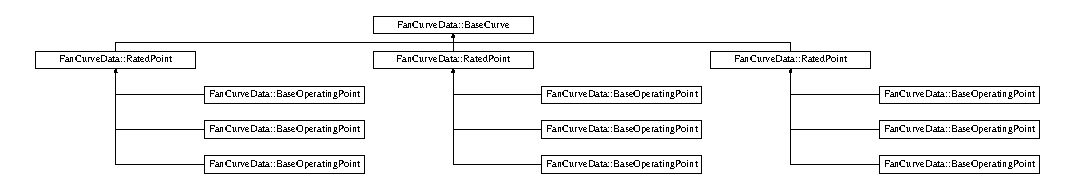
\includegraphics[height=2.111614cm]{da/d6e/struct_fan_curve_data_1_1_base_curve}
\end{center}
\end{figure}
\subsection*{Public Member Functions}
\begin{DoxyCompactItemize}
\item 
\mbox{\Hypertarget{struct_fan_curve_data_1_1_base_curve_a05d0e881e03368efcbab71997ff25f33}\label{struct_fan_curve_data_1_1_base_curve_a05d0e881e03368efcbab71997ff25f33}} 
{\bfseries Base\+Curve} (const double flow, const double pressure, const double power)
\item 
\mbox{\Hypertarget{struct_fan_curve_data_1_1_base_curve_a05d0e881e03368efcbab71997ff25f33}\label{struct_fan_curve_data_1_1_base_curve_a05d0e881e03368efcbab71997ff25f33}} 
{\bfseries Base\+Curve} (const double flow, const double pressure, const double power)
\item 
\mbox{\Hypertarget{struct_fan_curve_data_1_1_base_curve_a05d0e881e03368efcbab71997ff25f33}\label{struct_fan_curve_data_1_1_base_curve_a05d0e881e03368efcbab71997ff25f33}} 
{\bfseries Base\+Curve} (const double flow, const double pressure, const double power)
\end{DoxyCompactItemize}
\subsection*{Public Attributes}
\begin{DoxyCompactItemize}
\item 
\mbox{\Hypertarget{struct_fan_curve_data_1_1_base_curve_ab8b4cb389033aa5b58b49cebd8b672c6}\label{struct_fan_curve_data_1_1_base_curve_ab8b4cb389033aa5b58b49cebd8b672c6}} 
const double {\bfseries flow}
\item 
\mbox{\Hypertarget{struct_fan_curve_data_1_1_base_curve_a100c4a42e149760c3f3722dce0b679a3}\label{struct_fan_curve_data_1_1_base_curve_a100c4a42e149760c3f3722dce0b679a3}} 
const double {\bfseries pressure}
\item 
\mbox{\Hypertarget{struct_fan_curve_data_1_1_base_curve_a4282ce2c8fa4150ecf011c9edaa7cb9d}\label{struct_fan_curve_data_1_1_base_curve_a4282ce2c8fa4150ecf011c9edaa7cb9d}} 
const double {\bfseries power}
\end{DoxyCompactItemize}
\subsection*{Friends}
\begin{DoxyCompactItemize}
\item 
\mbox{\Hypertarget{struct_fan_curve_data_1_1_base_curve_a6c0df668730aa3a6673d279f2bbe7799}\label{struct_fan_curve_data_1_1_base_curve_a6c0df668730aa3a6673d279f2bbe7799}} 
class {\bfseries Fan\+Curve\+Data}
\end{DoxyCompactItemize}


\subsection{Detailed Description}


Definition at line 54 of file Fan\+Curve.\+h.



The documentation for this struct was generated from the following file\+:\begin{DoxyCompactItemize}
\item 
\+\_\+\+C\+Pack\+\_\+\+Packages/\+Darwin/\+S\+T\+G\+Z/amo\+\_\+tools\+\_\+suite-\/-\/\+Darwin-\/x86\+\_\+64/amo\+\_\+tools\+\_\+suite/include/fans/\hyperlink{___c_pack___packages_2_darwin_2_s_t_g_z_2amo__tools__suite--_darwin-x86__64_2amo__tools__suite_2include_2fans_2_fan_curve_8h}{Fan\+Curve.\+h}\end{DoxyCompactItemize}

\hypertarget{class_base_gas_density}{}\section{Base\+Gas\+Density Class Reference}
\label{class_base_gas_density}\index{Base\+Gas\+Density@{Base\+Gas\+Density}}
\subsection*{Public Types}
\begin{DoxyCompactItemize}
\item 
\mbox{\Hypertarget{class_base_gas_density_afb215e48f6193462521b7e8d47306ed3}\label{class_base_gas_density_afb215e48f6193462521b7e8d47306ed3}} 
enum {\bfseries Gas\+Type} \{ {\bfseries A\+IR}, 
{\bfseries S\+T\+A\+N\+D\+A\+R\+D\+A\+IR}, 
{\bfseries O\+T\+H\+E\+R\+G\+AS}
 \}
\item 
\mbox{\Hypertarget{class_base_gas_density_a54f846cc4683a49d3904a40fe2986772}\label{class_base_gas_density_a54f846cc4683a49d3904a40fe2986772}} 
enum {\bfseries Input\+Type} \{ {\bfseries D\+EW}, 
{\bfseries RH}, 
{\bfseries W\+ET}
 \}
\end{DoxyCompactItemize}
\subsection*{Public Member Functions}
\begin{DoxyCompactItemize}
\item 
\mbox{\Hypertarget{class_base_gas_density_a693fb58303fb2077aa5082b8f14dec84}\label{class_base_gas_density_a693fb58303fb2077aa5082b8f14dec84}} 
{\bfseries Base\+Gas\+Density} (double tdo, double pso, double pbo, double po, Gas\+Type gas\+Type)
\end{DoxyCompactItemize}
\subsection*{Friends}
\begin{DoxyCompactItemize}
\item 
\mbox{\Hypertarget{class_base_gas_density_a28ff438eefb65e97bddb4051dd0a0112}\label{class_base_gas_density_a28ff438eefb65e97bddb4051dd0a0112}} 
class {\bfseries Plane\+Data}
\item 
\mbox{\Hypertarget{class_base_gas_density_a0a305abd4183ca4b5d3adb1b563378d7}\label{class_base_gas_density_a0a305abd4183ca4b5d3adb1b563378d7}} 
class {\bfseries Fan}
\end{DoxyCompactItemize}


\subsection{Detailed Description}


Definition at line 22 of file Fan.\+h.



The documentation for this class was generated from the following files\+:\begin{DoxyCompactItemize}
\item 
include/fans/Fan.\+h\item 
src/fans/Fan.\+cpp\end{DoxyCompactItemize}

\hypertarget{struct_fan_curve_data_1_1_base_operating_point}{}\section{Fan\+Curve\+Data\+:\+:Base\+Operating\+Point Struct Reference}
\label{struct_fan_curve_data_1_1_base_operating_point}\index{Fan\+Curve\+Data\+::\+Base\+Operating\+Point@{Fan\+Curve\+Data\+::\+Base\+Operating\+Point}}
Inheritance diagram for Fan\+Curve\+Data\+:\+:Base\+Operating\+Point\+:\begin{figure}[H]
\begin{center}
\leavevmode
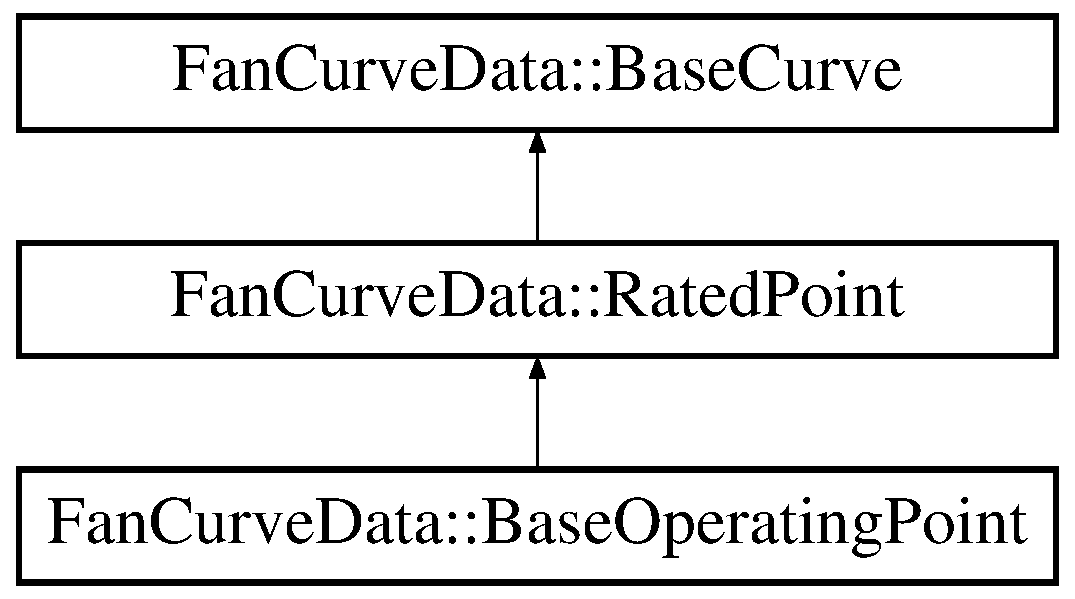
\includegraphics[height=2.111614cm]{d2/da0/struct_fan_curve_data_1_1_base_operating_point}
\end{center}
\end{figure}
\subsection*{Public Member Functions}
\begin{DoxyCompactItemize}
\item 
\mbox{\Hypertarget{struct_fan_curve_data_1_1_base_operating_point_a0260135ed464bc91143c620a1eeed78d}\label{struct_fan_curve_data_1_1_base_operating_point_a0260135ed464bc91143c620a1eeed78d}} 
{\bfseries Base\+Operating\+Point} (const double flow, const double pressure, const double power, const double density, const double speed, const double speed\+Corrected, const double pressure\+Barometric, const bool use\+Pt1\+Factor, const double pt1=0)
\item 
\mbox{\Hypertarget{struct_fan_curve_data_1_1_base_operating_point_a0260135ed464bc91143c620a1eeed78d}\label{struct_fan_curve_data_1_1_base_operating_point_a0260135ed464bc91143c620a1eeed78d}} 
{\bfseries Base\+Operating\+Point} (const double flow, const double pressure, const double power, const double density, const double speed, const double speed\+Corrected, const double pressure\+Barometric, const bool use\+Pt1\+Factor, const double pt1=0)
\item 
\mbox{\Hypertarget{struct_fan_curve_data_1_1_base_operating_point_a0260135ed464bc91143c620a1eeed78d}\label{struct_fan_curve_data_1_1_base_operating_point_a0260135ed464bc91143c620a1eeed78d}} 
{\bfseries Base\+Operating\+Point} (const double flow, const double pressure, const double power, const double density, const double speed, const double speed\+Corrected, const double pressure\+Barometric, const bool use\+Pt1\+Factor, const double pt1=0)
\end{DoxyCompactItemize}
\subsection*{Public Attributes}
\begin{DoxyCompactItemize}
\item 
\mbox{\Hypertarget{struct_fan_curve_data_1_1_base_operating_point_ab66cd337152255bf82b7ef98f828144b}\label{struct_fan_curve_data_1_1_base_operating_point_ab66cd337152255bf82b7ef98f828144b}} 
const double {\bfseries pressure\+Barometric}
\item 
\mbox{\Hypertarget{struct_fan_curve_data_1_1_base_operating_point_a4d09155765f22458b9feb10d77a188de}\label{struct_fan_curve_data_1_1_base_operating_point_a4d09155765f22458b9feb10d77a188de}} 
bool {\bfseries use\+Pt1\+Factor}
\item 
\mbox{\Hypertarget{struct_fan_curve_data_1_1_base_operating_point_ab349de155902de5f1a2c6dc6f48191b3}\label{struct_fan_curve_data_1_1_base_operating_point_ab349de155902de5f1a2c6dc6f48191b3}} 
const double {\bfseries pt1}
\end{DoxyCompactItemize}
\subsection*{Friends}
\begin{DoxyCompactItemize}
\item 
\mbox{\Hypertarget{struct_fan_curve_data_1_1_base_operating_point_a6c0df668730aa3a6673d279f2bbe7799}\label{struct_fan_curve_data_1_1_base_operating_point_a6c0df668730aa3a6673d279f2bbe7799}} 
class {\bfseries Fan\+Curve\+Data}
\end{DoxyCompactItemize}


\subsection{Detailed Description}


Definition at line 58 of file Fan\+Curve.\+h.



The documentation for this struct was generated from the following file\+:\begin{DoxyCompactItemize}
\item 
\+\_\+\+C\+Pack\+\_\+\+Packages/\+Darwin/\+S\+T\+G\+Z/amo\+\_\+tools\+\_\+suite-\/-\/\+Darwin-\/x86\+\_\+64-\/\+Debug/amo\+\_\+tools\+\_\+suite/include/fans/Fan\+Curve.\+h\end{DoxyCompactItemize}

\hypertarget{class_boiler}{}\section{Boiler Class Reference}
\label{class_boiler}\index{Boiler@{Boiler}}


{\ttfamily \#include $<$Boiler.\+h$>$}

\subsection*{Public Member Functions}
\begin{DoxyCompactItemize}
\item 
\hyperlink{class_boiler_adebe1dca06edc8dbca462e226b4dd9d5}{Boiler} (double deaerator\+Pressure, double combustion\+Efficiency, double blowdown\+Rate, double steam\+Pressure, \hyperlink{class_steam_properties_ae0294bedf7d178c2d8fb6aed0f62fbff}{Steam\+Properties\+::\+Thermodynamic\+Quantity} quantity\+Type, double quantity\+Value, double steam\+Mass\+Flow)
\item 
\mbox{\Hypertarget{class_boiler_a47e660b470ef7c2749102ae6873922e1}\label{class_boiler_a47e660b470ef7c2749102ae6873922e1}} 
\hyperlink{struct_steam_system_modeler_tool_1_1_fluid_properties}{Steam\+System\+Modeler\+Tool\+::\+Fluid\+Properties} const  \& {\bfseries get\+Steam\+Properties} () const
\item 
\mbox{\Hypertarget{class_boiler_ac48aa3ee13845cdf388085e73531cb66}\label{class_boiler_ac48aa3ee13845cdf388085e73531cb66}} 
\hyperlink{struct_steam_system_modeler_tool_1_1_fluid_properties}{Steam\+System\+Modeler\+Tool\+::\+Fluid\+Properties} const  \& {\bfseries get\+Blowdown\+Properties} () const
\item 
\mbox{\Hypertarget{class_boiler_a03e09f9469c746789f302c42c8dfe959}\label{class_boiler_a03e09f9469c746789f302c42c8dfe959}} 
\hyperlink{struct_steam_system_modeler_tool_1_1_fluid_properties}{Steam\+System\+Modeler\+Tool\+::\+Fluid\+Properties} const  \& {\bfseries get\+Feedwater\+Properties} () const
\item 
double \hyperlink{class_boiler_aad4786e7b68084e65a35dd6235517b8c}{get\+Deaerator\+Pressure} () const
\item 
double \hyperlink{class_boiler_a21c7423b756761c3216704b3f554feff}{get\+Combustion\+Efficiency} () const
\item 
double \hyperlink{class_boiler_aec9bf6eeed82d8d5f35284c65a3986e7}{get\+Blowdown\+Rate} () const
\item 
double \hyperlink{class_boiler_a99d4bbace6ef20bcbdc4b0cfcdc43213}{get\+Steam\+Pressure} () const
\item 
double \hyperlink{class_boiler_a78370a174135e6cc95abcd3b7ac2f947}{get\+Quantity\+Value} () const
\item 
double \hyperlink{class_boiler_a4101e71234995558a451dcab145b5fc9}{get\+Steam\+Mass\+Flow} () const
\item 
\hyperlink{class_steam_properties_ae0294bedf7d178c2d8fb6aed0f62fbff}{Steam\+Properties\+::\+Thermodynamic\+Quantity} \hyperlink{class_boiler_a26a71f789c9f9e05bd43a1ca0219f920}{get\+Quantity\+Type} () const
\item 
void \hyperlink{class_boiler_a56f422254606ebba1248ae0b4f8f0215}{set\+Deaerator\+Pressure} (double deaerator\+Pressure)
\item 
void \hyperlink{class_boiler_abef6bc48101f98f0650cb07fb1d51f74}{set\+Combustion\+Efficiency} (double combustion\+Efficiency)
\item 
void \hyperlink{class_boiler_a66c0e4c577dbd3f52dcf202e69a08371}{set\+Blowdown\+Rate} (double blowdown\+Rate)
\item 
void \hyperlink{class_boiler_a0a4619ff73c9969daebe3aa66ddad6be}{set\+Steam\+Pressure} (double steam\+Pressure)
\item 
void \hyperlink{class_boiler_ac3450d88dba124529d59baf62c39e14a}{set\+Quantity\+Value} (double quantity\+Value)
\item 
void \hyperlink{class_boiler_ada7af5896a2a4701d78a532dc9bc9892}{set\+Steam\+Mass\+Flow} (double steam\+Mass\+Flow)
\item 
void \hyperlink{class_boiler_a9c5b20cae6133c9174b12760f36d52c2}{set\+Quantity\+Type} (\hyperlink{class_steam_properties_ae0294bedf7d178c2d8fb6aed0f62fbff}{Steam\+Properties\+::\+Thermodynamic\+Quantity} quantity)
\item 
double \hyperlink{class_boiler_a8cc9ad5f1b36f5dcbcb225e9e3d13a39}{get\+Boiler\+Energy} () const
\item 
double \hyperlink{class_boiler_a55542a761669c842163b20932f9747d3}{get\+Fuel\+Energy} () const
\item 
\hyperlink{class_boiler_adebe1dca06edc8dbca462e226b4dd9d5}{Boiler} (double deaerator\+Pressure, double combustion\+Efficiency, double blowdown\+Rate, double steam\+Pressure, \hyperlink{class_steam_properties_ae0294bedf7d178c2d8fb6aed0f62fbff}{Steam\+Properties\+::\+Thermodynamic\+Quantity} quantity\+Type, double quantity\+Value, double steam\+Mass\+Flow)
\item 
\mbox{\Hypertarget{class_boiler_a47e660b470ef7c2749102ae6873922e1}\label{class_boiler_a47e660b470ef7c2749102ae6873922e1}} 
\hyperlink{struct_steam_system_modeler_tool_1_1_fluid_properties}{Steam\+System\+Modeler\+Tool\+::\+Fluid\+Properties} const  \& {\bfseries get\+Steam\+Properties} () const
\item 
\mbox{\Hypertarget{class_boiler_ac48aa3ee13845cdf388085e73531cb66}\label{class_boiler_ac48aa3ee13845cdf388085e73531cb66}} 
\hyperlink{struct_steam_system_modeler_tool_1_1_fluid_properties}{Steam\+System\+Modeler\+Tool\+::\+Fluid\+Properties} const  \& {\bfseries get\+Blowdown\+Properties} () const
\item 
\mbox{\Hypertarget{class_boiler_a03e09f9469c746789f302c42c8dfe959}\label{class_boiler_a03e09f9469c746789f302c42c8dfe959}} 
\hyperlink{struct_steam_system_modeler_tool_1_1_fluid_properties}{Steam\+System\+Modeler\+Tool\+::\+Fluid\+Properties} const  \& {\bfseries get\+Feedwater\+Properties} () const
\item 
double \hyperlink{class_boiler_aad4786e7b68084e65a35dd6235517b8c}{get\+Deaerator\+Pressure} () const
\item 
double \hyperlink{class_boiler_a21c7423b756761c3216704b3f554feff}{get\+Combustion\+Efficiency} () const
\item 
double \hyperlink{class_boiler_aec9bf6eeed82d8d5f35284c65a3986e7}{get\+Blowdown\+Rate} () const
\item 
double \hyperlink{class_boiler_a99d4bbace6ef20bcbdc4b0cfcdc43213}{get\+Steam\+Pressure} () const
\item 
double \hyperlink{class_boiler_a78370a174135e6cc95abcd3b7ac2f947}{get\+Quantity\+Value} () const
\item 
double \hyperlink{class_boiler_a4101e71234995558a451dcab145b5fc9}{get\+Steam\+Mass\+Flow} () const
\item 
\hyperlink{class_steam_properties_ae0294bedf7d178c2d8fb6aed0f62fbff}{Steam\+Properties\+::\+Thermodynamic\+Quantity} \hyperlink{class_boiler_a26a71f789c9f9e05bd43a1ca0219f920}{get\+Quantity\+Type} () const
\item 
void \hyperlink{class_boiler_a56f422254606ebba1248ae0b4f8f0215}{set\+Deaerator\+Pressure} (double deaerator\+Pressure)
\item 
void \hyperlink{class_boiler_abef6bc48101f98f0650cb07fb1d51f74}{set\+Combustion\+Efficiency} (double combustion\+Efficiency)
\item 
void \hyperlink{class_boiler_a66c0e4c577dbd3f52dcf202e69a08371}{set\+Blowdown\+Rate} (double blowdown\+Rate)
\item 
void \hyperlink{class_boiler_a0a4619ff73c9969daebe3aa66ddad6be}{set\+Steam\+Pressure} (double steam\+Pressure)
\item 
void \hyperlink{class_boiler_ac3450d88dba124529d59baf62c39e14a}{set\+Quantity\+Value} (double quantity\+Value)
\item 
void \hyperlink{class_boiler_ada7af5896a2a4701d78a532dc9bc9892}{set\+Steam\+Mass\+Flow} (double steam\+Mass\+Flow)
\item 
void \hyperlink{class_boiler_a9c5b20cae6133c9174b12760f36d52c2}{set\+Quantity\+Type} (\hyperlink{class_steam_properties_ae0294bedf7d178c2d8fb6aed0f62fbff}{Steam\+Properties\+::\+Thermodynamic\+Quantity} quantity)
\item 
double \hyperlink{class_boiler_a8cc9ad5f1b36f5dcbcb225e9e3d13a39}{get\+Boiler\+Energy} () const
\item 
double \hyperlink{class_boiler_a55542a761669c842163b20932f9747d3}{get\+Fuel\+Energy} () const
\item 
\hyperlink{class_boiler_adebe1dca06edc8dbca462e226b4dd9d5}{Boiler} (double deaerator\+Pressure, double combustion\+Efficiency, double blowdown\+Rate, double steam\+Pressure, \hyperlink{class_steam_properties_ae0294bedf7d178c2d8fb6aed0f62fbff}{Steam\+Properties\+::\+Thermodynamic\+Quantity} quantity\+Type, double quantity\+Value, double steam\+Mass\+Flow)
\item 
\mbox{\Hypertarget{class_boiler_a47e660b470ef7c2749102ae6873922e1}\label{class_boiler_a47e660b470ef7c2749102ae6873922e1}} 
\hyperlink{struct_steam_system_modeler_tool_1_1_fluid_properties}{Steam\+System\+Modeler\+Tool\+::\+Fluid\+Properties} const  \& {\bfseries get\+Steam\+Properties} () const
\item 
\mbox{\Hypertarget{class_boiler_ac48aa3ee13845cdf388085e73531cb66}\label{class_boiler_ac48aa3ee13845cdf388085e73531cb66}} 
\hyperlink{struct_steam_system_modeler_tool_1_1_fluid_properties}{Steam\+System\+Modeler\+Tool\+::\+Fluid\+Properties} const  \& {\bfseries get\+Blowdown\+Properties} () const
\item 
\mbox{\Hypertarget{class_boiler_a03e09f9469c746789f302c42c8dfe959}\label{class_boiler_a03e09f9469c746789f302c42c8dfe959}} 
\hyperlink{struct_steam_system_modeler_tool_1_1_fluid_properties}{Steam\+System\+Modeler\+Tool\+::\+Fluid\+Properties} const  \& {\bfseries get\+Feedwater\+Properties} () const
\item 
double \hyperlink{class_boiler_aad4786e7b68084e65a35dd6235517b8c}{get\+Deaerator\+Pressure} () const
\item 
double \hyperlink{class_boiler_a21c7423b756761c3216704b3f554feff}{get\+Combustion\+Efficiency} () const
\item 
double \hyperlink{class_boiler_aec9bf6eeed82d8d5f35284c65a3986e7}{get\+Blowdown\+Rate} () const
\item 
double \hyperlink{class_boiler_a99d4bbace6ef20bcbdc4b0cfcdc43213}{get\+Steam\+Pressure} () const
\item 
double \hyperlink{class_boiler_a78370a174135e6cc95abcd3b7ac2f947}{get\+Quantity\+Value} () const
\item 
double \hyperlink{class_boiler_a4101e71234995558a451dcab145b5fc9}{get\+Steam\+Mass\+Flow} () const
\item 
\hyperlink{class_steam_properties_ae0294bedf7d178c2d8fb6aed0f62fbff}{Steam\+Properties\+::\+Thermodynamic\+Quantity} \hyperlink{class_boiler_a26a71f789c9f9e05bd43a1ca0219f920}{get\+Quantity\+Type} () const
\item 
void \hyperlink{class_boiler_a56f422254606ebba1248ae0b4f8f0215}{set\+Deaerator\+Pressure} (double deaerator\+Pressure)
\item 
void \hyperlink{class_boiler_abef6bc48101f98f0650cb07fb1d51f74}{set\+Combustion\+Efficiency} (double combustion\+Efficiency)
\item 
void \hyperlink{class_boiler_a66c0e4c577dbd3f52dcf202e69a08371}{set\+Blowdown\+Rate} (double blowdown\+Rate)
\item 
void \hyperlink{class_boiler_a0a4619ff73c9969daebe3aa66ddad6be}{set\+Steam\+Pressure} (double steam\+Pressure)
\item 
void \hyperlink{class_boiler_ac3450d88dba124529d59baf62c39e14a}{set\+Quantity\+Value} (double quantity\+Value)
\item 
void \hyperlink{class_boiler_ada7af5896a2a4701d78a532dc9bc9892}{set\+Steam\+Mass\+Flow} (double steam\+Mass\+Flow)
\item 
void \hyperlink{class_boiler_a9c5b20cae6133c9174b12760f36d52c2}{set\+Quantity\+Type} (\hyperlink{class_steam_properties_ae0294bedf7d178c2d8fb6aed0f62fbff}{Steam\+Properties\+::\+Thermodynamic\+Quantity} quantity)
\item 
double \hyperlink{class_boiler_a8cc9ad5f1b36f5dcbcb225e9e3d13a39}{get\+Boiler\+Energy} () const
\item 
double \hyperlink{class_boiler_a55542a761669c842163b20932f9747d3}{get\+Fuel\+Energy} () const
\end{DoxyCompactItemize}


\subsection{Detailed Description}
\hyperlink{class_boiler}{Boiler} calculator class Used to determines the amount of fuel energy required to produce steam with specified properties at a given flow rate using general boiler operational characteristics 

Definition at line 23 of file Boiler.\+h.



\subsection{Constructor \& Destructor Documentation}
\mbox{\Hypertarget{class_boiler_adebe1dca06edc8dbca462e226b4dd9d5}\label{class_boiler_adebe1dca06edc8dbca462e226b4dd9d5}} 
\index{Boiler@{Boiler}!Boiler@{Boiler}}
\index{Boiler@{Boiler}!Boiler@{Boiler}}
\subsubsection{\texorpdfstring{Boiler()}{Boiler()}\hspace{0.1cm}{\footnotesize\ttfamily [1/3]}}
{\footnotesize\ttfamily Boiler\+::\+Boiler (\begin{DoxyParamCaption}\item[{double}]{deaerator\+Pressure,  }\item[{double}]{combustion\+Efficiency,  }\item[{double}]{blowdown\+Rate,  }\item[{double}]{steam\+Pressure,  }\item[{\hyperlink{class_steam_properties_ae0294bedf7d178c2d8fb6aed0f62fbff}{Steam\+Properties\+::\+Thermodynamic\+Quantity}}]{quantity\+Type,  }\item[{double}]{quantity\+Value,  }\item[{double}]{steam\+Mass\+Flow }\end{DoxyParamCaption})}

Constructor for the boiler calculator


\begin{DoxyParams}{Parameters}
{\em deaerator\+Pressure} & double, pressure of deaerator in M\+Pa \\
\hline
{\em combustion\+Efficiency} & double, combustion efficiency of the boiler as \% \\
\hline
{\em blowdown\+Rate} & double, blowdown rate as a \% of inlet mass flow \\
\hline
{\em steam\+Pressure} & double, pressure of steam in M\+Pa \\
\hline
{\em quantity\+Type} & \hyperlink{class_steam_properties_ae0294bedf7d178c2d8fb6aed0f62fbff}{Steam\+Properties\+::\+Thermodynamic\+Quantity}, type of quantity (either temperature in K, enthalpy in k\+J/kg, entropy in k\+J/kg/K, or quality -\/ unitless) \\
\hline
{\em quantity\+Value} & double, value of the quantity (either temperature in K, enthalpy in k\+J/kg, entropy in k\+J/kg/K, or quality -\/ unitless) \\
\hline
{\em steam\+Mass\+Flow} & double, steam mass flow in kg/hr \\
\hline
\end{DoxyParams}


Definition at line 12 of file Boiler.\+cpp.

\mbox{\Hypertarget{class_boiler_adebe1dca06edc8dbca462e226b4dd9d5}\label{class_boiler_adebe1dca06edc8dbca462e226b4dd9d5}} 
\index{Boiler@{Boiler}!Boiler@{Boiler}}
\index{Boiler@{Boiler}!Boiler@{Boiler}}
\subsubsection{\texorpdfstring{Boiler()}{Boiler()}\hspace{0.1cm}{\footnotesize\ttfamily [2/3]}}
{\footnotesize\ttfamily Boiler\+::\+Boiler (\begin{DoxyParamCaption}\item[{double}]{deaerator\+Pressure,  }\item[{double}]{combustion\+Efficiency,  }\item[{double}]{blowdown\+Rate,  }\item[{double}]{steam\+Pressure,  }\item[{\hyperlink{class_steam_properties_ae0294bedf7d178c2d8fb6aed0f62fbff}{Steam\+Properties\+::\+Thermodynamic\+Quantity}}]{quantity\+Type,  }\item[{double}]{quantity\+Value,  }\item[{double}]{steam\+Mass\+Flow }\end{DoxyParamCaption})}

Constructor for the boiler calculator


\begin{DoxyParams}{Parameters}
{\em deaerator\+Pressure} & double, pressure of deaerator in M\+Pa \\
\hline
{\em combustion\+Efficiency} & double, combustion efficiency of the boiler as \% \\
\hline
{\em blowdown\+Rate} & double, blowdown rate as a \% of inlet mass flow \\
\hline
{\em steam\+Pressure} & double, pressure of steam in M\+Pa \\
\hline
{\em quantity\+Type} & \hyperlink{class_steam_properties_ae0294bedf7d178c2d8fb6aed0f62fbff}{Steam\+Properties\+::\+Thermodynamic\+Quantity}, type of quantity (either temperature in K, enthalpy in k\+J/kg, entropy in k\+J/kg/K, or quality -\/ unitless) \\
\hline
{\em quantity\+Value} & double, value of the quantity (either temperature in K, enthalpy in k\+J/kg, entropy in k\+J/kg/K, or quality -\/ unitless) \\
\hline
{\em steam\+Mass\+Flow} & double, steam mass flow in kg/hr \\
\hline
\end{DoxyParams}
\mbox{\Hypertarget{class_boiler_adebe1dca06edc8dbca462e226b4dd9d5}\label{class_boiler_adebe1dca06edc8dbca462e226b4dd9d5}} 
\index{Boiler@{Boiler}!Boiler@{Boiler}}
\index{Boiler@{Boiler}!Boiler@{Boiler}}
\subsubsection{\texorpdfstring{Boiler()}{Boiler()}\hspace{0.1cm}{\footnotesize\ttfamily [3/3]}}
{\footnotesize\ttfamily Boiler\+::\+Boiler (\begin{DoxyParamCaption}\item[{double}]{deaerator\+Pressure,  }\item[{double}]{combustion\+Efficiency,  }\item[{double}]{blowdown\+Rate,  }\item[{double}]{steam\+Pressure,  }\item[{\hyperlink{class_steam_properties_ae0294bedf7d178c2d8fb6aed0f62fbff}{Steam\+Properties\+::\+Thermodynamic\+Quantity}}]{quantity\+Type,  }\item[{double}]{quantity\+Value,  }\item[{double}]{steam\+Mass\+Flow }\end{DoxyParamCaption})}

Constructor for the boiler calculator


\begin{DoxyParams}{Parameters}
{\em deaerator\+Pressure} & double, pressure of deaerator in M\+Pa \\
\hline
{\em combustion\+Efficiency} & double, combustion efficiency of the boiler as \% \\
\hline
{\em blowdown\+Rate} & double, blowdown rate as a \% of inlet mass flow \\
\hline
{\em steam\+Pressure} & double, pressure of steam in M\+Pa \\
\hline
{\em quantity\+Type} & \hyperlink{class_steam_properties_ae0294bedf7d178c2d8fb6aed0f62fbff}{Steam\+Properties\+::\+Thermodynamic\+Quantity}, type of quantity (either temperature in K, enthalpy in k\+J/kg, entropy in k\+J/kg/K, or quality -\/ unitless) \\
\hline
{\em quantity\+Value} & double, value of the quantity (either temperature in K, enthalpy in k\+J/kg, entropy in k\+J/kg/K, or quality -\/ unitless) \\
\hline
{\em steam\+Mass\+Flow} & double, steam mass flow in kg/hr \\
\hline
\end{DoxyParams}


\subsection{Member Function Documentation}
\mbox{\Hypertarget{class_boiler_aec9bf6eeed82d8d5f35284c65a3986e7}\label{class_boiler_aec9bf6eeed82d8d5f35284c65a3986e7}} 
\index{Boiler@{Boiler}!get\+Blowdown\+Rate@{get\+Blowdown\+Rate}}
\index{get\+Blowdown\+Rate@{get\+Blowdown\+Rate}!Boiler@{Boiler}}
\subsubsection{\texorpdfstring{get\+Blowdown\+Rate()}{getBlowdownRate()}\hspace{0.1cm}{\footnotesize\ttfamily [1/3]}}
{\footnotesize\ttfamily double Boiler\+::get\+Blowdown\+Rate (\begin{DoxyParamCaption}{ }\end{DoxyParamCaption}) const}

Gets the blowdown rate \begin{DoxyReturn}{Returns}
double, blowdown rate as a \% of inlet mass flow 
\end{DoxyReturn}
\mbox{\Hypertarget{class_boiler_aec9bf6eeed82d8d5f35284c65a3986e7}\label{class_boiler_aec9bf6eeed82d8d5f35284c65a3986e7}} 
\index{Boiler@{Boiler}!get\+Blowdown\+Rate@{get\+Blowdown\+Rate}}
\index{get\+Blowdown\+Rate@{get\+Blowdown\+Rate}!Boiler@{Boiler}}
\subsubsection{\texorpdfstring{get\+Blowdown\+Rate()}{getBlowdownRate()}\hspace{0.1cm}{\footnotesize\ttfamily [2/3]}}
{\footnotesize\ttfamily double Boiler\+::get\+Blowdown\+Rate (\begin{DoxyParamCaption}{ }\end{DoxyParamCaption}) const}

Gets the blowdown rate \begin{DoxyReturn}{Returns}
double, blowdown rate as a \% of inlet mass flow 
\end{DoxyReturn}


Definition at line 41 of file Boiler.\+cpp.

\mbox{\Hypertarget{class_boiler_aec9bf6eeed82d8d5f35284c65a3986e7}\label{class_boiler_aec9bf6eeed82d8d5f35284c65a3986e7}} 
\index{Boiler@{Boiler}!get\+Blowdown\+Rate@{get\+Blowdown\+Rate}}
\index{get\+Blowdown\+Rate@{get\+Blowdown\+Rate}!Boiler@{Boiler}}
\subsubsection{\texorpdfstring{get\+Blowdown\+Rate()}{getBlowdownRate()}\hspace{0.1cm}{\footnotesize\ttfamily [3/3]}}
{\footnotesize\ttfamily double Boiler\+::get\+Blowdown\+Rate (\begin{DoxyParamCaption}{ }\end{DoxyParamCaption}) const}

Gets the blowdown rate \begin{DoxyReturn}{Returns}
double, blowdown rate as a \% of inlet mass flow 
\end{DoxyReturn}
\mbox{\Hypertarget{class_boiler_a8cc9ad5f1b36f5dcbcb225e9e3d13a39}\label{class_boiler_a8cc9ad5f1b36f5dcbcb225e9e3d13a39}} 
\index{Boiler@{Boiler}!get\+Boiler\+Energy@{get\+Boiler\+Energy}}
\index{get\+Boiler\+Energy@{get\+Boiler\+Energy}!Boiler@{Boiler}}
\subsubsection{\texorpdfstring{get\+Boiler\+Energy()}{getBoilerEnergy()}\hspace{0.1cm}{\footnotesize\ttfamily [1/3]}}
{\footnotesize\ttfamily double Boiler\+::get\+Boiler\+Energy (\begin{DoxyParamCaption}{ }\end{DoxyParamCaption}) const\hspace{0.3cm}{\ttfamily [inline]}}

Returns the boiler energy \begin{DoxyReturn}{Returns}
double, boiler energy in MJ 
\end{DoxyReturn}


Definition at line 135 of file Boiler.\+h.

\mbox{\Hypertarget{class_boiler_a8cc9ad5f1b36f5dcbcb225e9e3d13a39}\label{class_boiler_a8cc9ad5f1b36f5dcbcb225e9e3d13a39}} 
\index{Boiler@{Boiler}!get\+Boiler\+Energy@{get\+Boiler\+Energy}}
\index{get\+Boiler\+Energy@{get\+Boiler\+Energy}!Boiler@{Boiler}}
\subsubsection{\texorpdfstring{get\+Boiler\+Energy()}{getBoilerEnergy()}\hspace{0.1cm}{\footnotesize\ttfamily [2/3]}}
{\footnotesize\ttfamily double Boiler\+::get\+Boiler\+Energy (\begin{DoxyParamCaption}{ }\end{DoxyParamCaption}) const\hspace{0.3cm}{\ttfamily [inline]}}

Returns the boiler energy \begin{DoxyReturn}{Returns}
double, boiler energy in MJ 
\end{DoxyReturn}


Definition at line 135 of file Boiler.\+h.

\mbox{\Hypertarget{class_boiler_a8cc9ad5f1b36f5dcbcb225e9e3d13a39}\label{class_boiler_a8cc9ad5f1b36f5dcbcb225e9e3d13a39}} 
\index{Boiler@{Boiler}!get\+Boiler\+Energy@{get\+Boiler\+Energy}}
\index{get\+Boiler\+Energy@{get\+Boiler\+Energy}!Boiler@{Boiler}}
\subsubsection{\texorpdfstring{get\+Boiler\+Energy()}{getBoilerEnergy()}\hspace{0.1cm}{\footnotesize\ttfamily [3/3]}}
{\footnotesize\ttfamily double Boiler\+::get\+Boiler\+Energy (\begin{DoxyParamCaption}{ }\end{DoxyParamCaption}) const\hspace{0.3cm}{\ttfamily [inline]}}

Returns the boiler energy \begin{DoxyReturn}{Returns}
double, boiler energy in MJ 
\end{DoxyReturn}


Definition at line 135 of file Boiler.\+h.

\mbox{\Hypertarget{class_boiler_a21c7423b756761c3216704b3f554feff}\label{class_boiler_a21c7423b756761c3216704b3f554feff}} 
\index{Boiler@{Boiler}!get\+Combustion\+Efficiency@{get\+Combustion\+Efficiency}}
\index{get\+Combustion\+Efficiency@{get\+Combustion\+Efficiency}!Boiler@{Boiler}}
\subsubsection{\texorpdfstring{get\+Combustion\+Efficiency()}{getCombustionEfficiency()}\hspace{0.1cm}{\footnotesize\ttfamily [1/3]}}
{\footnotesize\ttfamily double Boiler\+::get\+Combustion\+Efficiency (\begin{DoxyParamCaption}{ }\end{DoxyParamCaption}) const}

Gets the combustion efficiency of the boiler \begin{DoxyReturn}{Returns}
double, combustion efficiency as \% 
\end{DoxyReturn}


Definition at line 40 of file Boiler.\+cpp.

\mbox{\Hypertarget{class_boiler_a21c7423b756761c3216704b3f554feff}\label{class_boiler_a21c7423b756761c3216704b3f554feff}} 
\index{Boiler@{Boiler}!get\+Combustion\+Efficiency@{get\+Combustion\+Efficiency}}
\index{get\+Combustion\+Efficiency@{get\+Combustion\+Efficiency}!Boiler@{Boiler}}
\subsubsection{\texorpdfstring{get\+Combustion\+Efficiency()}{getCombustionEfficiency()}\hspace{0.1cm}{\footnotesize\ttfamily [2/3]}}
{\footnotesize\ttfamily double Boiler\+::get\+Combustion\+Efficiency (\begin{DoxyParamCaption}{ }\end{DoxyParamCaption}) const}

Gets the combustion efficiency of the boiler \begin{DoxyReturn}{Returns}
double, combustion efficiency as \% 
\end{DoxyReturn}
\mbox{\Hypertarget{class_boiler_a21c7423b756761c3216704b3f554feff}\label{class_boiler_a21c7423b756761c3216704b3f554feff}} 
\index{Boiler@{Boiler}!get\+Combustion\+Efficiency@{get\+Combustion\+Efficiency}}
\index{get\+Combustion\+Efficiency@{get\+Combustion\+Efficiency}!Boiler@{Boiler}}
\subsubsection{\texorpdfstring{get\+Combustion\+Efficiency()}{getCombustionEfficiency()}\hspace{0.1cm}{\footnotesize\ttfamily [3/3]}}
{\footnotesize\ttfamily double Boiler\+::get\+Combustion\+Efficiency (\begin{DoxyParamCaption}{ }\end{DoxyParamCaption}) const}

Gets the combustion efficiency of the boiler \begin{DoxyReturn}{Returns}
double, combustion efficiency as \% 
\end{DoxyReturn}
\mbox{\Hypertarget{class_boiler_aad4786e7b68084e65a35dd6235517b8c}\label{class_boiler_aad4786e7b68084e65a35dd6235517b8c}} 
\index{Boiler@{Boiler}!get\+Deaerator\+Pressure@{get\+Deaerator\+Pressure}}
\index{get\+Deaerator\+Pressure@{get\+Deaerator\+Pressure}!Boiler@{Boiler}}
\subsubsection{\texorpdfstring{get\+Deaerator\+Pressure()}{getDeaeratorPressure()}\hspace{0.1cm}{\footnotesize\ttfamily [1/3]}}
{\footnotesize\ttfamily double Boiler\+::get\+Deaerator\+Pressure (\begin{DoxyParamCaption}{ }\end{DoxyParamCaption}) const}

Gets the deaerator pressure \begin{DoxyReturn}{Returns}
double, pressure of the deaerator in M\+Pa 
\end{DoxyReturn}


Definition at line 39 of file Boiler.\+cpp.

\mbox{\Hypertarget{class_boiler_aad4786e7b68084e65a35dd6235517b8c}\label{class_boiler_aad4786e7b68084e65a35dd6235517b8c}} 
\index{Boiler@{Boiler}!get\+Deaerator\+Pressure@{get\+Deaerator\+Pressure}}
\index{get\+Deaerator\+Pressure@{get\+Deaerator\+Pressure}!Boiler@{Boiler}}
\subsubsection{\texorpdfstring{get\+Deaerator\+Pressure()}{getDeaeratorPressure()}\hspace{0.1cm}{\footnotesize\ttfamily [2/3]}}
{\footnotesize\ttfamily double Boiler\+::get\+Deaerator\+Pressure (\begin{DoxyParamCaption}{ }\end{DoxyParamCaption}) const}

Gets the deaerator pressure \begin{DoxyReturn}{Returns}
double, pressure of the deaerator in M\+Pa 
\end{DoxyReturn}
\mbox{\Hypertarget{class_boiler_aad4786e7b68084e65a35dd6235517b8c}\label{class_boiler_aad4786e7b68084e65a35dd6235517b8c}} 
\index{Boiler@{Boiler}!get\+Deaerator\+Pressure@{get\+Deaerator\+Pressure}}
\index{get\+Deaerator\+Pressure@{get\+Deaerator\+Pressure}!Boiler@{Boiler}}
\subsubsection{\texorpdfstring{get\+Deaerator\+Pressure()}{getDeaeratorPressure()}\hspace{0.1cm}{\footnotesize\ttfamily [3/3]}}
{\footnotesize\ttfamily double Boiler\+::get\+Deaerator\+Pressure (\begin{DoxyParamCaption}{ }\end{DoxyParamCaption}) const}

Gets the deaerator pressure \begin{DoxyReturn}{Returns}
double, pressure of the deaerator in M\+Pa 
\end{DoxyReturn}
\mbox{\Hypertarget{class_boiler_a55542a761669c842163b20932f9747d3}\label{class_boiler_a55542a761669c842163b20932f9747d3}} 
\index{Boiler@{Boiler}!get\+Fuel\+Energy@{get\+Fuel\+Energy}}
\index{get\+Fuel\+Energy@{get\+Fuel\+Energy}!Boiler@{Boiler}}
\subsubsection{\texorpdfstring{get\+Fuel\+Energy()}{getFuelEnergy()}\hspace{0.1cm}{\footnotesize\ttfamily [1/3]}}
{\footnotesize\ttfamily double Boiler\+::get\+Fuel\+Energy (\begin{DoxyParamCaption}{ }\end{DoxyParamCaption}) const\hspace{0.3cm}{\ttfamily [inline]}}

Returns the fuel energy \begin{DoxyReturn}{Returns}
double, fuel energy in MJ 
\end{DoxyReturn}


Definition at line 141 of file Boiler.\+h.

\mbox{\Hypertarget{class_boiler_a55542a761669c842163b20932f9747d3}\label{class_boiler_a55542a761669c842163b20932f9747d3}} 
\index{Boiler@{Boiler}!get\+Fuel\+Energy@{get\+Fuel\+Energy}}
\index{get\+Fuel\+Energy@{get\+Fuel\+Energy}!Boiler@{Boiler}}
\subsubsection{\texorpdfstring{get\+Fuel\+Energy()}{getFuelEnergy()}\hspace{0.1cm}{\footnotesize\ttfamily [2/3]}}
{\footnotesize\ttfamily double Boiler\+::get\+Fuel\+Energy (\begin{DoxyParamCaption}{ }\end{DoxyParamCaption}) const\hspace{0.3cm}{\ttfamily [inline]}}

Returns the fuel energy \begin{DoxyReturn}{Returns}
double, fuel energy in MJ 
\end{DoxyReturn}


Definition at line 141 of file Boiler.\+h.

\mbox{\Hypertarget{class_boiler_a55542a761669c842163b20932f9747d3}\label{class_boiler_a55542a761669c842163b20932f9747d3}} 
\index{Boiler@{Boiler}!get\+Fuel\+Energy@{get\+Fuel\+Energy}}
\index{get\+Fuel\+Energy@{get\+Fuel\+Energy}!Boiler@{Boiler}}
\subsubsection{\texorpdfstring{get\+Fuel\+Energy()}{getFuelEnergy()}\hspace{0.1cm}{\footnotesize\ttfamily [3/3]}}
{\footnotesize\ttfamily double Boiler\+::get\+Fuel\+Energy (\begin{DoxyParamCaption}{ }\end{DoxyParamCaption}) const\hspace{0.3cm}{\ttfamily [inline]}}

Returns the fuel energy \begin{DoxyReturn}{Returns}
double, fuel energy in MJ 
\end{DoxyReturn}


Definition at line 141 of file Boiler.\+h.

\mbox{\Hypertarget{class_boiler_a26a71f789c9f9e05bd43a1ca0219f920}\label{class_boiler_a26a71f789c9f9e05bd43a1ca0219f920}} 
\index{Boiler@{Boiler}!get\+Quantity\+Type@{get\+Quantity\+Type}}
\index{get\+Quantity\+Type@{get\+Quantity\+Type}!Boiler@{Boiler}}
\subsubsection{\texorpdfstring{get\+Quantity\+Type()}{getQuantityType()}\hspace{0.1cm}{\footnotesize\ttfamily [1/3]}}
{\footnotesize\ttfamily \hyperlink{class_steam_properties_ae0294bedf7d178c2d8fb6aed0f62fbff}{Steam\+Properties\+::\+Thermodynamic\+Quantity} Boiler\+::get\+Quantity\+Type (\begin{DoxyParamCaption}{ }\end{DoxyParamCaption}) const}

Gets the quantity type \begin{DoxyReturn}{Returns}
\hyperlink{class_steam_properties_ae0294bedf7d178c2d8fb6aed0f62fbff}{Steam\+Properties\+::\+Thermodynamic\+Quantity}, type of quantity (either temperature in K, enthalpy in k\+J/kg, entropy in k\+J/kg/K, or quality -\/ unitless) 
\end{DoxyReturn}


Definition at line 45 of file Boiler.\+cpp.

\mbox{\Hypertarget{class_boiler_a26a71f789c9f9e05bd43a1ca0219f920}\label{class_boiler_a26a71f789c9f9e05bd43a1ca0219f920}} 
\index{Boiler@{Boiler}!get\+Quantity\+Type@{get\+Quantity\+Type}}
\index{get\+Quantity\+Type@{get\+Quantity\+Type}!Boiler@{Boiler}}
\subsubsection{\texorpdfstring{get\+Quantity\+Type()}{getQuantityType()}\hspace{0.1cm}{\footnotesize\ttfamily [2/3]}}
{\footnotesize\ttfamily \hyperlink{class_steam_properties_ae0294bedf7d178c2d8fb6aed0f62fbff}{Steam\+Properties\+::\+Thermodynamic\+Quantity} Boiler\+::get\+Quantity\+Type (\begin{DoxyParamCaption}{ }\end{DoxyParamCaption}) const}

Gets the quantity type \begin{DoxyReturn}{Returns}
\hyperlink{class_steam_properties_ae0294bedf7d178c2d8fb6aed0f62fbff}{Steam\+Properties\+::\+Thermodynamic\+Quantity}, type of quantity (either temperature in K, enthalpy in k\+J/kg, entropy in k\+J/kg/K, or quality -\/ unitless) 
\end{DoxyReturn}
\mbox{\Hypertarget{class_boiler_a26a71f789c9f9e05bd43a1ca0219f920}\label{class_boiler_a26a71f789c9f9e05bd43a1ca0219f920}} 
\index{Boiler@{Boiler}!get\+Quantity\+Type@{get\+Quantity\+Type}}
\index{get\+Quantity\+Type@{get\+Quantity\+Type}!Boiler@{Boiler}}
\subsubsection{\texorpdfstring{get\+Quantity\+Type()}{getQuantityType()}\hspace{0.1cm}{\footnotesize\ttfamily [3/3]}}
{\footnotesize\ttfamily \hyperlink{class_steam_properties_ae0294bedf7d178c2d8fb6aed0f62fbff}{Steam\+Properties\+::\+Thermodynamic\+Quantity} Boiler\+::get\+Quantity\+Type (\begin{DoxyParamCaption}{ }\end{DoxyParamCaption}) const}

Gets the quantity type \begin{DoxyReturn}{Returns}
\hyperlink{class_steam_properties_ae0294bedf7d178c2d8fb6aed0f62fbff}{Steam\+Properties\+::\+Thermodynamic\+Quantity}, type of quantity (either temperature in K, enthalpy in k\+J/kg, entropy in k\+J/kg/K, or quality -\/ unitless) 
\end{DoxyReturn}
\mbox{\Hypertarget{class_boiler_a78370a174135e6cc95abcd3b7ac2f947}\label{class_boiler_a78370a174135e6cc95abcd3b7ac2f947}} 
\index{Boiler@{Boiler}!get\+Quantity\+Value@{get\+Quantity\+Value}}
\index{get\+Quantity\+Value@{get\+Quantity\+Value}!Boiler@{Boiler}}
\subsubsection{\texorpdfstring{get\+Quantity\+Value()}{getQuantityValue()}\hspace{0.1cm}{\footnotesize\ttfamily [1/3]}}
{\footnotesize\ttfamily double Boiler\+::get\+Quantity\+Value (\begin{DoxyParamCaption}{ }\end{DoxyParamCaption}) const}

Gets the quantity value \begin{DoxyReturn}{Returns}
double, value of quantity (either temperature in K, enthalpy in k\+J/kg, entropy in k\+J/kg/K, or quality -\/ unitless) 
\end{DoxyReturn}


Definition at line 43 of file Boiler.\+cpp.

\mbox{\Hypertarget{class_boiler_a78370a174135e6cc95abcd3b7ac2f947}\label{class_boiler_a78370a174135e6cc95abcd3b7ac2f947}} 
\index{Boiler@{Boiler}!get\+Quantity\+Value@{get\+Quantity\+Value}}
\index{get\+Quantity\+Value@{get\+Quantity\+Value}!Boiler@{Boiler}}
\subsubsection{\texorpdfstring{get\+Quantity\+Value()}{getQuantityValue()}\hspace{0.1cm}{\footnotesize\ttfamily [2/3]}}
{\footnotesize\ttfamily double Boiler\+::get\+Quantity\+Value (\begin{DoxyParamCaption}{ }\end{DoxyParamCaption}) const}

Gets the quantity value \begin{DoxyReturn}{Returns}
double, value of quantity (either temperature in K, enthalpy in k\+J/kg, entropy in k\+J/kg/K, or quality -\/ unitless) 
\end{DoxyReturn}
\mbox{\Hypertarget{class_boiler_a78370a174135e6cc95abcd3b7ac2f947}\label{class_boiler_a78370a174135e6cc95abcd3b7ac2f947}} 
\index{Boiler@{Boiler}!get\+Quantity\+Value@{get\+Quantity\+Value}}
\index{get\+Quantity\+Value@{get\+Quantity\+Value}!Boiler@{Boiler}}
\subsubsection{\texorpdfstring{get\+Quantity\+Value()}{getQuantityValue()}\hspace{0.1cm}{\footnotesize\ttfamily [3/3]}}
{\footnotesize\ttfamily double Boiler\+::get\+Quantity\+Value (\begin{DoxyParamCaption}{ }\end{DoxyParamCaption}) const}

Gets the quantity value \begin{DoxyReturn}{Returns}
double, value of quantity (either temperature in K, enthalpy in k\+J/kg, entropy in k\+J/kg/K, or quality -\/ unitless) 
\end{DoxyReturn}
\mbox{\Hypertarget{class_boiler_a4101e71234995558a451dcab145b5fc9}\label{class_boiler_a4101e71234995558a451dcab145b5fc9}} 
\index{Boiler@{Boiler}!get\+Steam\+Mass\+Flow@{get\+Steam\+Mass\+Flow}}
\index{get\+Steam\+Mass\+Flow@{get\+Steam\+Mass\+Flow}!Boiler@{Boiler}}
\subsubsection{\texorpdfstring{get\+Steam\+Mass\+Flow()}{getSteamMassFlow()}\hspace{0.1cm}{\footnotesize\ttfamily [1/3]}}
{\footnotesize\ttfamily double Boiler\+::get\+Steam\+Mass\+Flow (\begin{DoxyParamCaption}{ }\end{DoxyParamCaption}) const}

Gets the steam mass flow \begin{DoxyReturn}{Returns}
double, mass flow of steam in kg/hr 
\end{DoxyReturn}


Definition at line 44 of file Boiler.\+cpp.

\mbox{\Hypertarget{class_boiler_a4101e71234995558a451dcab145b5fc9}\label{class_boiler_a4101e71234995558a451dcab145b5fc9}} 
\index{Boiler@{Boiler}!get\+Steam\+Mass\+Flow@{get\+Steam\+Mass\+Flow}}
\index{get\+Steam\+Mass\+Flow@{get\+Steam\+Mass\+Flow}!Boiler@{Boiler}}
\subsubsection{\texorpdfstring{get\+Steam\+Mass\+Flow()}{getSteamMassFlow()}\hspace{0.1cm}{\footnotesize\ttfamily [2/3]}}
{\footnotesize\ttfamily double Boiler\+::get\+Steam\+Mass\+Flow (\begin{DoxyParamCaption}{ }\end{DoxyParamCaption}) const}

Gets the steam mass flow \begin{DoxyReturn}{Returns}
double, mass flow of steam in kg/hr 
\end{DoxyReturn}
\mbox{\Hypertarget{class_boiler_a4101e71234995558a451dcab145b5fc9}\label{class_boiler_a4101e71234995558a451dcab145b5fc9}} 
\index{Boiler@{Boiler}!get\+Steam\+Mass\+Flow@{get\+Steam\+Mass\+Flow}}
\index{get\+Steam\+Mass\+Flow@{get\+Steam\+Mass\+Flow}!Boiler@{Boiler}}
\subsubsection{\texorpdfstring{get\+Steam\+Mass\+Flow()}{getSteamMassFlow()}\hspace{0.1cm}{\footnotesize\ttfamily [3/3]}}
{\footnotesize\ttfamily double Boiler\+::get\+Steam\+Mass\+Flow (\begin{DoxyParamCaption}{ }\end{DoxyParamCaption}) const}

Gets the steam mass flow \begin{DoxyReturn}{Returns}
double, mass flow of steam in kg/hr 
\end{DoxyReturn}
\mbox{\Hypertarget{class_boiler_a99d4bbace6ef20bcbdc4b0cfcdc43213}\label{class_boiler_a99d4bbace6ef20bcbdc4b0cfcdc43213}} 
\index{Boiler@{Boiler}!get\+Steam\+Pressure@{get\+Steam\+Pressure}}
\index{get\+Steam\+Pressure@{get\+Steam\+Pressure}!Boiler@{Boiler}}
\subsubsection{\texorpdfstring{get\+Steam\+Pressure()}{getSteamPressure()}\hspace{0.1cm}{\footnotesize\ttfamily [1/3]}}
{\footnotesize\ttfamily double Boiler\+::get\+Steam\+Pressure (\begin{DoxyParamCaption}{ }\end{DoxyParamCaption}) const}

Gets the steam pressure \begin{DoxyReturn}{Returns}
double, pressure of steam in M\+Pa 
\end{DoxyReturn}
\mbox{\Hypertarget{class_boiler_a99d4bbace6ef20bcbdc4b0cfcdc43213}\label{class_boiler_a99d4bbace6ef20bcbdc4b0cfcdc43213}} 
\index{Boiler@{Boiler}!get\+Steam\+Pressure@{get\+Steam\+Pressure}}
\index{get\+Steam\+Pressure@{get\+Steam\+Pressure}!Boiler@{Boiler}}
\subsubsection{\texorpdfstring{get\+Steam\+Pressure()}{getSteamPressure()}\hspace{0.1cm}{\footnotesize\ttfamily [2/3]}}
{\footnotesize\ttfamily double Boiler\+::get\+Steam\+Pressure (\begin{DoxyParamCaption}{ }\end{DoxyParamCaption}) const}

Gets the steam pressure \begin{DoxyReturn}{Returns}
double, pressure of steam in M\+Pa 
\end{DoxyReturn}
\mbox{\Hypertarget{class_boiler_a99d4bbace6ef20bcbdc4b0cfcdc43213}\label{class_boiler_a99d4bbace6ef20bcbdc4b0cfcdc43213}} 
\index{Boiler@{Boiler}!get\+Steam\+Pressure@{get\+Steam\+Pressure}}
\index{get\+Steam\+Pressure@{get\+Steam\+Pressure}!Boiler@{Boiler}}
\subsubsection{\texorpdfstring{get\+Steam\+Pressure()}{getSteamPressure()}\hspace{0.1cm}{\footnotesize\ttfamily [3/3]}}
{\footnotesize\ttfamily double Boiler\+::get\+Steam\+Pressure (\begin{DoxyParamCaption}{ }\end{DoxyParamCaption}) const}

Gets the steam pressure \begin{DoxyReturn}{Returns}
double, pressure of steam in M\+Pa 
\end{DoxyReturn}


Definition at line 42 of file Boiler.\+cpp.

\mbox{\Hypertarget{class_boiler_a66c0e4c577dbd3f52dcf202e69a08371}\label{class_boiler_a66c0e4c577dbd3f52dcf202e69a08371}} 
\index{Boiler@{Boiler}!set\+Blowdown\+Rate@{set\+Blowdown\+Rate}}
\index{set\+Blowdown\+Rate@{set\+Blowdown\+Rate}!Boiler@{Boiler}}
\subsubsection{\texorpdfstring{set\+Blowdown\+Rate()}{setBlowdownRate()}\hspace{0.1cm}{\footnotesize\ttfamily [1/3]}}
{\footnotesize\ttfamily void Boiler\+::set\+Blowdown\+Rate (\begin{DoxyParamCaption}\item[{double}]{blowdown\+Rate }\end{DoxyParamCaption})}

Sets the blowdown rate 
\begin{DoxyParams}{Parameters}
{\em blowdown\+Rate} & double, blowdown rate as a \% of inlet mass flow \\
\hline
\end{DoxyParams}
\mbox{\Hypertarget{class_boiler_a66c0e4c577dbd3f52dcf202e69a08371}\label{class_boiler_a66c0e4c577dbd3f52dcf202e69a08371}} 
\index{Boiler@{Boiler}!set\+Blowdown\+Rate@{set\+Blowdown\+Rate}}
\index{set\+Blowdown\+Rate@{set\+Blowdown\+Rate}!Boiler@{Boiler}}
\subsubsection{\texorpdfstring{set\+Blowdown\+Rate()}{setBlowdownRate()}\hspace{0.1cm}{\footnotesize\ttfamily [2/3]}}
{\footnotesize\ttfamily void Boiler\+::set\+Blowdown\+Rate (\begin{DoxyParamCaption}\item[{double}]{blowdown\+Rate }\end{DoxyParamCaption})}

Sets the blowdown rate 
\begin{DoxyParams}{Parameters}
{\em blowdown\+Rate} & double, blowdown rate as a \% of inlet mass flow \\
\hline
\end{DoxyParams}
\mbox{\Hypertarget{class_boiler_a66c0e4c577dbd3f52dcf202e69a08371}\label{class_boiler_a66c0e4c577dbd3f52dcf202e69a08371}} 
\index{Boiler@{Boiler}!set\+Blowdown\+Rate@{set\+Blowdown\+Rate}}
\index{set\+Blowdown\+Rate@{set\+Blowdown\+Rate}!Boiler@{Boiler}}
\subsubsection{\texorpdfstring{set\+Blowdown\+Rate()}{setBlowdownRate()}\hspace{0.1cm}{\footnotesize\ttfamily [3/3]}}
{\footnotesize\ttfamily void Boiler\+::set\+Blowdown\+Rate (\begin{DoxyParamCaption}\item[{double}]{blowdown\+Rate }\end{DoxyParamCaption})}

Sets the blowdown rate 
\begin{DoxyParams}{Parameters}
{\em blowdown\+Rate} & double, blowdown rate as a \% of inlet mass flow \\
\hline
\end{DoxyParams}


Definition at line 57 of file Boiler.\+cpp.

\mbox{\Hypertarget{class_boiler_abef6bc48101f98f0650cb07fb1d51f74}\label{class_boiler_abef6bc48101f98f0650cb07fb1d51f74}} 
\index{Boiler@{Boiler}!set\+Combustion\+Efficiency@{set\+Combustion\+Efficiency}}
\index{set\+Combustion\+Efficiency@{set\+Combustion\+Efficiency}!Boiler@{Boiler}}
\subsubsection{\texorpdfstring{set\+Combustion\+Efficiency()}{setCombustionEfficiency()}\hspace{0.1cm}{\footnotesize\ttfamily [1/3]}}
{\footnotesize\ttfamily void Boiler\+::set\+Combustion\+Efficiency (\begin{DoxyParamCaption}\item[{double}]{combustion\+Efficiency }\end{DoxyParamCaption})}

Sets the combustion efficiency of the boiler 
\begin{DoxyParams}{Parameters}
{\em combustion\+Efficiency} & double, combustion efficiency as \% \\
\hline
\end{DoxyParams}


Definition at line 52 of file Boiler.\+cpp.

\mbox{\Hypertarget{class_boiler_abef6bc48101f98f0650cb07fb1d51f74}\label{class_boiler_abef6bc48101f98f0650cb07fb1d51f74}} 
\index{Boiler@{Boiler}!set\+Combustion\+Efficiency@{set\+Combustion\+Efficiency}}
\index{set\+Combustion\+Efficiency@{set\+Combustion\+Efficiency}!Boiler@{Boiler}}
\subsubsection{\texorpdfstring{set\+Combustion\+Efficiency()}{setCombustionEfficiency()}\hspace{0.1cm}{\footnotesize\ttfamily [2/3]}}
{\footnotesize\ttfamily void Boiler\+::set\+Combustion\+Efficiency (\begin{DoxyParamCaption}\item[{double}]{combustion\+Efficiency }\end{DoxyParamCaption})}

Sets the combustion efficiency of the boiler 
\begin{DoxyParams}{Parameters}
{\em combustion\+Efficiency} & double, combustion efficiency as \% \\
\hline
\end{DoxyParams}
\mbox{\Hypertarget{class_boiler_abef6bc48101f98f0650cb07fb1d51f74}\label{class_boiler_abef6bc48101f98f0650cb07fb1d51f74}} 
\index{Boiler@{Boiler}!set\+Combustion\+Efficiency@{set\+Combustion\+Efficiency}}
\index{set\+Combustion\+Efficiency@{set\+Combustion\+Efficiency}!Boiler@{Boiler}}
\subsubsection{\texorpdfstring{set\+Combustion\+Efficiency()}{setCombustionEfficiency()}\hspace{0.1cm}{\footnotesize\ttfamily [3/3]}}
{\footnotesize\ttfamily void Boiler\+::set\+Combustion\+Efficiency (\begin{DoxyParamCaption}\item[{double}]{combustion\+Efficiency }\end{DoxyParamCaption})}

Sets the combustion efficiency of the boiler 
\begin{DoxyParams}{Parameters}
{\em combustion\+Efficiency} & double, combustion efficiency as \% \\
\hline
\end{DoxyParams}
\mbox{\Hypertarget{class_boiler_a56f422254606ebba1248ae0b4f8f0215}\label{class_boiler_a56f422254606ebba1248ae0b4f8f0215}} 
\index{Boiler@{Boiler}!set\+Deaerator\+Pressure@{set\+Deaerator\+Pressure}}
\index{set\+Deaerator\+Pressure@{set\+Deaerator\+Pressure}!Boiler@{Boiler}}
\subsubsection{\texorpdfstring{set\+Deaerator\+Pressure()}{setDeaeratorPressure()}\hspace{0.1cm}{\footnotesize\ttfamily [1/3]}}
{\footnotesize\ttfamily void Boiler\+::set\+Deaerator\+Pressure (\begin{DoxyParamCaption}\item[{double}]{deaerator\+Pressure }\end{DoxyParamCaption})}

Sets the deaerator pressure 
\begin{DoxyParams}{Parameters}
{\em deaerator\+Pressure} & double, pressure of the deaerator in M\+Pa \\
\hline
\end{DoxyParams}
\mbox{\Hypertarget{class_boiler_a56f422254606ebba1248ae0b4f8f0215}\label{class_boiler_a56f422254606ebba1248ae0b4f8f0215}} 
\index{Boiler@{Boiler}!set\+Deaerator\+Pressure@{set\+Deaerator\+Pressure}}
\index{set\+Deaerator\+Pressure@{set\+Deaerator\+Pressure}!Boiler@{Boiler}}
\subsubsection{\texorpdfstring{set\+Deaerator\+Pressure()}{setDeaeratorPressure()}\hspace{0.1cm}{\footnotesize\ttfamily [2/3]}}
{\footnotesize\ttfamily void Boiler\+::set\+Deaerator\+Pressure (\begin{DoxyParamCaption}\item[{double}]{deaerator\+Pressure }\end{DoxyParamCaption})}

Sets the deaerator pressure 
\begin{DoxyParams}{Parameters}
{\em deaerator\+Pressure} & double, pressure of the deaerator in M\+Pa \\
\hline
\end{DoxyParams}
\mbox{\Hypertarget{class_boiler_a56f422254606ebba1248ae0b4f8f0215}\label{class_boiler_a56f422254606ebba1248ae0b4f8f0215}} 
\index{Boiler@{Boiler}!set\+Deaerator\+Pressure@{set\+Deaerator\+Pressure}}
\index{set\+Deaerator\+Pressure@{set\+Deaerator\+Pressure}!Boiler@{Boiler}}
\subsubsection{\texorpdfstring{set\+Deaerator\+Pressure()}{setDeaeratorPressure()}\hspace{0.1cm}{\footnotesize\ttfamily [3/3]}}
{\footnotesize\ttfamily void Boiler\+::set\+Deaerator\+Pressure (\begin{DoxyParamCaption}\item[{double}]{deaerator\+Pressure }\end{DoxyParamCaption})}

Sets the deaerator pressure 
\begin{DoxyParams}{Parameters}
{\em deaerator\+Pressure} & double, pressure of the deaerator in M\+Pa \\
\hline
\end{DoxyParams}


Definition at line 47 of file Boiler.\+cpp.

\mbox{\Hypertarget{class_boiler_a9c5b20cae6133c9174b12760f36d52c2}\label{class_boiler_a9c5b20cae6133c9174b12760f36d52c2}} 
\index{Boiler@{Boiler}!set\+Quantity\+Type@{set\+Quantity\+Type}}
\index{set\+Quantity\+Type@{set\+Quantity\+Type}!Boiler@{Boiler}}
\subsubsection{\texorpdfstring{set\+Quantity\+Type()}{setQuantityType()}\hspace{0.1cm}{\footnotesize\ttfamily [1/3]}}
{\footnotesize\ttfamily void Boiler\+::set\+Quantity\+Type (\begin{DoxyParamCaption}\item[{\hyperlink{class_steam_properties_ae0294bedf7d178c2d8fb6aed0f62fbff}{Steam\+Properties\+::\+Thermodynamic\+Quantity}}]{quantity }\end{DoxyParamCaption})}

Sets the quantity type 
\begin{DoxyParams}{Parameters}
{\em quantity\+Type} & \hyperlink{class_steam_properties_ae0294bedf7d178c2d8fb6aed0f62fbff}{Steam\+Properties\+::\+Thermodynamic\+Quantity}, type of quantity (either temperature in K, enthalpy in k\+J/kg, entropy in k\+J/kg/K, or quality -\/ unitless) \\
\hline
\end{DoxyParams}


Definition at line 67 of file Boiler.\+cpp.

\mbox{\Hypertarget{class_boiler_a9c5b20cae6133c9174b12760f36d52c2}\label{class_boiler_a9c5b20cae6133c9174b12760f36d52c2}} 
\index{Boiler@{Boiler}!set\+Quantity\+Type@{set\+Quantity\+Type}}
\index{set\+Quantity\+Type@{set\+Quantity\+Type}!Boiler@{Boiler}}
\subsubsection{\texorpdfstring{set\+Quantity\+Type()}{setQuantityType()}\hspace{0.1cm}{\footnotesize\ttfamily [2/3]}}
{\footnotesize\ttfamily void Boiler\+::set\+Quantity\+Type (\begin{DoxyParamCaption}\item[{\hyperlink{class_steam_properties_ae0294bedf7d178c2d8fb6aed0f62fbff}{Steam\+Properties\+::\+Thermodynamic\+Quantity}}]{quantity }\end{DoxyParamCaption})}

Sets the quantity type 
\begin{DoxyParams}{Parameters}
{\em quantity\+Type} & \hyperlink{class_steam_properties_ae0294bedf7d178c2d8fb6aed0f62fbff}{Steam\+Properties\+::\+Thermodynamic\+Quantity}, type of quantity (either temperature in K, enthalpy in k\+J/kg, entropy in k\+J/kg/K, or quality -\/ unitless) \\
\hline
\end{DoxyParams}
\mbox{\Hypertarget{class_boiler_a9c5b20cae6133c9174b12760f36d52c2}\label{class_boiler_a9c5b20cae6133c9174b12760f36d52c2}} 
\index{Boiler@{Boiler}!set\+Quantity\+Type@{set\+Quantity\+Type}}
\index{set\+Quantity\+Type@{set\+Quantity\+Type}!Boiler@{Boiler}}
\subsubsection{\texorpdfstring{set\+Quantity\+Type()}{setQuantityType()}\hspace{0.1cm}{\footnotesize\ttfamily [3/3]}}
{\footnotesize\ttfamily void Boiler\+::set\+Quantity\+Type (\begin{DoxyParamCaption}\item[{\hyperlink{class_steam_properties_ae0294bedf7d178c2d8fb6aed0f62fbff}{Steam\+Properties\+::\+Thermodynamic\+Quantity}}]{quantity }\end{DoxyParamCaption})}

Sets the quantity type 
\begin{DoxyParams}{Parameters}
{\em quantity\+Type} & \hyperlink{class_steam_properties_ae0294bedf7d178c2d8fb6aed0f62fbff}{Steam\+Properties\+::\+Thermodynamic\+Quantity}, type of quantity (either temperature in K, enthalpy in k\+J/kg, entropy in k\+J/kg/K, or quality -\/ unitless) \\
\hline
\end{DoxyParams}
\mbox{\Hypertarget{class_boiler_ac3450d88dba124529d59baf62c39e14a}\label{class_boiler_ac3450d88dba124529d59baf62c39e14a}} 
\index{Boiler@{Boiler}!set\+Quantity\+Value@{set\+Quantity\+Value}}
\index{set\+Quantity\+Value@{set\+Quantity\+Value}!Boiler@{Boiler}}
\subsubsection{\texorpdfstring{set\+Quantity\+Value()}{setQuantityValue()}\hspace{0.1cm}{\footnotesize\ttfamily [1/3]}}
{\footnotesize\ttfamily void Boiler\+::set\+Quantity\+Value (\begin{DoxyParamCaption}\item[{double}]{quantity\+Value }\end{DoxyParamCaption})}

Sets the quantity value 
\begin{DoxyParams}{Parameters}
{\em quantity\+Value} & double, value of quantity (either temperature in K, enthalpy in k\+J/kg, entropy in k\+J/kg/K, or quality -\/ unitless) \\
\hline
\end{DoxyParams}
\mbox{\Hypertarget{class_boiler_ac3450d88dba124529d59baf62c39e14a}\label{class_boiler_ac3450d88dba124529d59baf62c39e14a}} 
\index{Boiler@{Boiler}!set\+Quantity\+Value@{set\+Quantity\+Value}}
\index{set\+Quantity\+Value@{set\+Quantity\+Value}!Boiler@{Boiler}}
\subsubsection{\texorpdfstring{set\+Quantity\+Value()}{setQuantityValue()}\hspace{0.1cm}{\footnotesize\ttfamily [2/3]}}
{\footnotesize\ttfamily void Boiler\+::set\+Quantity\+Value (\begin{DoxyParamCaption}\item[{double}]{quantity\+Value }\end{DoxyParamCaption})}

Sets the quantity value 
\begin{DoxyParams}{Parameters}
{\em quantity\+Value} & double, value of quantity (either temperature in K, enthalpy in k\+J/kg, entropy in k\+J/kg/K, or quality -\/ unitless) \\
\hline
\end{DoxyParams}


Definition at line 72 of file Boiler.\+cpp.

\mbox{\Hypertarget{class_boiler_ac3450d88dba124529d59baf62c39e14a}\label{class_boiler_ac3450d88dba124529d59baf62c39e14a}} 
\index{Boiler@{Boiler}!set\+Quantity\+Value@{set\+Quantity\+Value}}
\index{set\+Quantity\+Value@{set\+Quantity\+Value}!Boiler@{Boiler}}
\subsubsection{\texorpdfstring{set\+Quantity\+Value()}{setQuantityValue()}\hspace{0.1cm}{\footnotesize\ttfamily [3/3]}}
{\footnotesize\ttfamily void Boiler\+::set\+Quantity\+Value (\begin{DoxyParamCaption}\item[{double}]{quantity\+Value }\end{DoxyParamCaption})}

Sets the quantity value 
\begin{DoxyParams}{Parameters}
{\em quantity\+Value} & double, value of quantity (either temperature in K, enthalpy in k\+J/kg, entropy in k\+J/kg/K, or quality -\/ unitless) \\
\hline
\end{DoxyParams}
\mbox{\Hypertarget{class_boiler_ada7af5896a2a4701d78a532dc9bc9892}\label{class_boiler_ada7af5896a2a4701d78a532dc9bc9892}} 
\index{Boiler@{Boiler}!set\+Steam\+Mass\+Flow@{set\+Steam\+Mass\+Flow}}
\index{set\+Steam\+Mass\+Flow@{set\+Steam\+Mass\+Flow}!Boiler@{Boiler}}
\subsubsection{\texorpdfstring{set\+Steam\+Mass\+Flow()}{setSteamMassFlow()}\hspace{0.1cm}{\footnotesize\ttfamily [1/3]}}
{\footnotesize\ttfamily void Boiler\+::set\+Steam\+Mass\+Flow (\begin{DoxyParamCaption}\item[{double}]{steam\+Mass\+Flow }\end{DoxyParamCaption})}

Sets the steam mass flow 
\begin{DoxyParams}{Parameters}
{\em steam\+Mass\+Flow} & double, mass flow of steam in kg/hr \\
\hline
\end{DoxyParams}


Definition at line 77 of file Boiler.\+cpp.

\mbox{\Hypertarget{class_boiler_ada7af5896a2a4701d78a532dc9bc9892}\label{class_boiler_ada7af5896a2a4701d78a532dc9bc9892}} 
\index{Boiler@{Boiler}!set\+Steam\+Mass\+Flow@{set\+Steam\+Mass\+Flow}}
\index{set\+Steam\+Mass\+Flow@{set\+Steam\+Mass\+Flow}!Boiler@{Boiler}}
\subsubsection{\texorpdfstring{set\+Steam\+Mass\+Flow()}{setSteamMassFlow()}\hspace{0.1cm}{\footnotesize\ttfamily [2/3]}}
{\footnotesize\ttfamily void Boiler\+::set\+Steam\+Mass\+Flow (\begin{DoxyParamCaption}\item[{double}]{steam\+Mass\+Flow }\end{DoxyParamCaption})}

Sets the steam mass flow 
\begin{DoxyParams}{Parameters}
{\em steam\+Mass\+Flow} & double, mass flow of steam in kg/hr \\
\hline
\end{DoxyParams}
\mbox{\Hypertarget{class_boiler_ada7af5896a2a4701d78a532dc9bc9892}\label{class_boiler_ada7af5896a2a4701d78a532dc9bc9892}} 
\index{Boiler@{Boiler}!set\+Steam\+Mass\+Flow@{set\+Steam\+Mass\+Flow}}
\index{set\+Steam\+Mass\+Flow@{set\+Steam\+Mass\+Flow}!Boiler@{Boiler}}
\subsubsection{\texorpdfstring{set\+Steam\+Mass\+Flow()}{setSteamMassFlow()}\hspace{0.1cm}{\footnotesize\ttfamily [3/3]}}
{\footnotesize\ttfamily void Boiler\+::set\+Steam\+Mass\+Flow (\begin{DoxyParamCaption}\item[{double}]{steam\+Mass\+Flow }\end{DoxyParamCaption})}

Sets the steam mass flow 
\begin{DoxyParams}{Parameters}
{\em steam\+Mass\+Flow} & double, mass flow of steam in kg/hr \\
\hline
\end{DoxyParams}
\mbox{\Hypertarget{class_boiler_a0a4619ff73c9969daebe3aa66ddad6be}\label{class_boiler_a0a4619ff73c9969daebe3aa66ddad6be}} 
\index{Boiler@{Boiler}!set\+Steam\+Pressure@{set\+Steam\+Pressure}}
\index{set\+Steam\+Pressure@{set\+Steam\+Pressure}!Boiler@{Boiler}}
\subsubsection{\texorpdfstring{set\+Steam\+Pressure()}{setSteamPressure()}\hspace{0.1cm}{\footnotesize\ttfamily [1/3]}}
{\footnotesize\ttfamily void Boiler\+::set\+Steam\+Pressure (\begin{DoxyParamCaption}\item[{double}]{steam\+Pressure }\end{DoxyParamCaption})}

Sets the steam pressure 
\begin{DoxyParams}{Parameters}
{\em steam\+Pressure} & double, pressure of steam in M\+Pa \\
\hline
\end{DoxyParams}
\mbox{\Hypertarget{class_boiler_a0a4619ff73c9969daebe3aa66ddad6be}\label{class_boiler_a0a4619ff73c9969daebe3aa66ddad6be}} 
\index{Boiler@{Boiler}!set\+Steam\+Pressure@{set\+Steam\+Pressure}}
\index{set\+Steam\+Pressure@{set\+Steam\+Pressure}!Boiler@{Boiler}}
\subsubsection{\texorpdfstring{set\+Steam\+Pressure()}{setSteamPressure()}\hspace{0.1cm}{\footnotesize\ttfamily [2/3]}}
{\footnotesize\ttfamily void Boiler\+::set\+Steam\+Pressure (\begin{DoxyParamCaption}\item[{double}]{steam\+Pressure }\end{DoxyParamCaption})}

Sets the steam pressure 
\begin{DoxyParams}{Parameters}
{\em steam\+Pressure} & double, pressure of steam in M\+Pa \\
\hline
\end{DoxyParams}
\mbox{\Hypertarget{class_boiler_a0a4619ff73c9969daebe3aa66ddad6be}\label{class_boiler_a0a4619ff73c9969daebe3aa66ddad6be}} 
\index{Boiler@{Boiler}!set\+Steam\+Pressure@{set\+Steam\+Pressure}}
\index{set\+Steam\+Pressure@{set\+Steam\+Pressure}!Boiler@{Boiler}}
\subsubsection{\texorpdfstring{set\+Steam\+Pressure()}{setSteamPressure()}\hspace{0.1cm}{\footnotesize\ttfamily [3/3]}}
{\footnotesize\ttfamily void Boiler\+::set\+Steam\+Pressure (\begin{DoxyParamCaption}\item[{double}]{steam\+Pressure }\end{DoxyParamCaption})}

Sets the steam pressure 
\begin{DoxyParams}{Parameters}
{\em steam\+Pressure} & double, pressure of steam in M\+Pa \\
\hline
\end{DoxyParams}


Definition at line 62 of file Boiler.\+cpp.



The documentation for this class was generated from the following files\+:\begin{DoxyCompactItemize}
\item 
\+\_\+\+C\+Pack\+\_\+\+Packages/\+Darwin/\+S\+T\+G\+Z/amo\+\_\+tools\+\_\+suite-\/-\/\+Darwin-\/x86\+\_\+64-\/\+Debug/amo\+\_\+tools\+\_\+suite/include/ssmt/\hyperlink{___c_pack___packages_2_darwin_2_s_t_g_z_2amo__tools__suite--_darwin-x86__64-_debug_2amo__tools__7b788f9ca0770ad621a2356b855bf0c2}{Boiler.\+h}\item 
src/ssmt/\hyperlink{_boiler_8cpp}{Boiler.\+cpp}\end{DoxyCompactItemize}

\hypertarget{class_c_h_p}{}\section{C\+HP Class Reference}
\label{class_c_h_p}\index{C\+HP@{C\+HP}}
\subsection*{Public Types}
\begin{DoxyCompactItemize}
\item 
\mbox{\Hypertarget{class_c_h_p_ac82f530412021ace928a7e95c1295d06}\label{class_c_h_p_ac82f530412021ace928a7e95c1295d06}} 
enum {\bfseries Option} \{ \newline
{\bfseries Percent\+Avgk\+Wh\+Electric\+Cost\+Avoided}, 
{\bfseries Standby\+Rate}, 
{\bfseries Percent\+Avgk\+Wh\+Electric\+Cost\+Avoided}, 
{\bfseries Standby\+Rate}, 
\newline
{\bfseries Percent\+Avgk\+Wh\+Electric\+Cost\+Avoided}, 
{\bfseries Standby\+Rate}
 \}
\item 
\mbox{\Hypertarget{class_c_h_p_ac82f530412021ace928a7e95c1295d06}\label{class_c_h_p_ac82f530412021ace928a7e95c1295d06}} 
enum {\bfseries Option} \{ \newline
{\bfseries Percent\+Avgk\+Wh\+Electric\+Cost\+Avoided}, 
{\bfseries Standby\+Rate}, 
{\bfseries Percent\+Avgk\+Wh\+Electric\+Cost\+Avoided}, 
{\bfseries Standby\+Rate}, 
\newline
{\bfseries Percent\+Avgk\+Wh\+Electric\+Cost\+Avoided}, 
{\bfseries Standby\+Rate}
 \}
\item 
\mbox{\Hypertarget{class_c_h_p_ac82f530412021ace928a7e95c1295d06}\label{class_c_h_p_ac82f530412021ace928a7e95c1295d06}} 
enum {\bfseries Option} \{ \newline
{\bfseries Percent\+Avgk\+Wh\+Electric\+Cost\+Avoided}, 
{\bfseries Standby\+Rate}, 
{\bfseries Percent\+Avgk\+Wh\+Electric\+Cost\+Avoided}, 
{\bfseries Standby\+Rate}, 
\newline
{\bfseries Percent\+Avgk\+Wh\+Electric\+Cost\+Avoided}, 
{\bfseries Standby\+Rate}
 \}
\end{DoxyCompactItemize}
\subsection*{Public Member Functions}
\begin{DoxyCompactItemize}
\item 
\mbox{\Hypertarget{class_c_h_p_aea45a2afd5189214fbf720e53d587640}\label{class_c_h_p_aea45a2afd5189214fbf720e53d587640}} 
{\bfseries C\+HP} (double annual\+Operating\+Hours, double annual\+Electricity\+Consumption, double annual\+Thermal\+Demand, double boiler\+Thermal\+Fuel\+Costs, double avg\+Electricity\+Costs, Option calculation\+Option, double boiler\+Thermal\+Fuel\+Costs\+C\+H\+Pcase, double C\+H\+Pfuel\+Costs, double percent\+Avgk\+Wh\+Electric\+Cost\+Avoided\+Or\+Standby\+Rate, double displaced\+Thermal\+Efficiency, double chp\+Availability, double thermal\+Utilization)
\item 
\mbox{\Hypertarget{class_c_h_p_a9b448b253454087f9e98124aa716715f}\label{class_c_h_p_a9b448b253454087f9e98124aa716715f}} 
std\+::unordered\+\_\+map$<$ std\+::string, double $>$ const  \& {\bfseries get\+Cost\+Info} () const
\item 
\mbox{\Hypertarget{class_c_h_p_aeeb03f1f40db034babf883a1e00ed2a3}\label{class_c_h_p_aeeb03f1f40db034babf883a1e00ed2a3}} 
double {\bfseries get\+Annual\+Operating\+Hours} () const
\item 
\mbox{\Hypertarget{class_c_h_p_a37d544d03c45668a9dc5d502cdcb6137}\label{class_c_h_p_a37d544d03c45668a9dc5d502cdcb6137}} 
double {\bfseries get\+Annual\+Electricity\+Consumption} () const
\item 
\mbox{\Hypertarget{class_c_h_p_a849a576483b92b131ebfc0615e1e0bdb}\label{class_c_h_p_a849a576483b92b131ebfc0615e1e0bdb}} 
double {\bfseries get\+Annual\+Thermal\+Demand} () const
\item 
\mbox{\Hypertarget{class_c_h_p_a9f6c6638b1be7c2df8ba4b406c3b2b94}\label{class_c_h_p_a9f6c6638b1be7c2df8ba4b406c3b2b94}} 
double {\bfseries get\+Boiler\+Thermal\+Fuel\+Costs} () const
\item 
\mbox{\Hypertarget{class_c_h_p_a00929ba5d10367258dc1dc437eda88e3}\label{class_c_h_p_a00929ba5d10367258dc1dc437eda88e3}} 
double {\bfseries get\+Chp\+Fuel\+Costs} () const
\item 
\mbox{\Hypertarget{class_c_h_p_a2bc5ac0eb3d7ce42f77f26b3973f6c9f}\label{class_c_h_p_a2bc5ac0eb3d7ce42f77f26b3973f6c9f}} 
double {\bfseries get\+Avg\+Electricity\+Costs} () const
\item 
\mbox{\Hypertarget{class_c_h_p_a858f0201818f637331e0d06d3171bee7}\label{class_c_h_p_a858f0201818f637331e0d06d3171bee7}} 
Option {\bfseries get\+Calculation\+Option} () const
\item 
\mbox{\Hypertarget{class_c_h_p_ace1d96aacf328bd62f01e0eceaae19f6}\label{class_c_h_p_ace1d96aacf328bd62f01e0eceaae19f6}} 
double {\bfseries get\+Boiler\+Thermal\+Fuel\+Costs\+C\+H\+Pcase} () const
\item 
\mbox{\Hypertarget{class_c_h_p_ad79607b304d1e50a9421de043b7a9e7b}\label{class_c_h_p_ad79607b304d1e50a9421de043b7a9e7b}} 
double {\bfseries get\+Percent\+Avgk\+Wh\+Electric\+Cost\+Avoided} () const
\item 
\mbox{\Hypertarget{class_c_h_p_a195f0ffe163404077b56a5e5db8eb59c}\label{class_c_h_p_a195f0ffe163404077b56a5e5db8eb59c}} 
double {\bfseries get\+Standby\+Rate} () const
\item 
\mbox{\Hypertarget{class_c_h_p_a66b1b0e6a0d7f3181b3c1dfb590ab523}\label{class_c_h_p_a66b1b0e6a0d7f3181b3c1dfb590ab523}} 
double {\bfseries get\+Displaced\+Thermal\+Efficiency} () const
\item 
\mbox{\Hypertarget{class_c_h_p_a1d38e08a7815211361d334263832cad6}\label{class_c_h_p_a1d38e08a7815211361d334263832cad6}} 
double {\bfseries get\+Chp\+Electric\+Efficiency} () const
\item 
\mbox{\Hypertarget{class_c_h_p_a13e271f59d6315088416123c6e794e09}\label{class_c_h_p_a13e271f59d6315088416123c6e794e09}} 
double {\bfseries get\+Chp\+Thermal\+Output} () const
\item 
\mbox{\Hypertarget{class_c_h_p_abd1ea13cd48f5af48799891a52634340}\label{class_c_h_p_abd1ea13cd48f5af48799891a52634340}} 
double {\bfseries get\+Chp\+Availability} () const
\item 
\mbox{\Hypertarget{class_c_h_p_aa27fd9e66e208e6b3f28fdfe182d6c32}\label{class_c_h_p_aa27fd9e66e208e6b3f28fdfe182d6c32}} 
double {\bfseries get\+Thermal\+Utilization} () const
\item 
\mbox{\Hypertarget{class_c_h_p_a79f9a97a010669c5ffed9339c54a36c6}\label{class_c_h_p_a79f9a97a010669c5ffed9339c54a36c6}} 
double {\bfseries get\+Avg\+Power\+Demand} () const
\item 
\mbox{\Hypertarget{class_c_h_p_a5f8975488324e4aa3517c9e01334f4bf}\label{class_c_h_p_a5f8975488324e4aa3517c9e01334f4bf}} 
double {\bfseries get\+Avg\+Thermal\+Demand} () const
\item 
\mbox{\Hypertarget{class_c_h_p_a317f3df613b61f401bc5c4b69fddd0cf}\label{class_c_h_p_a317f3df613b61f401bc5c4b69fddd0cf}} 
double {\bfseries get\+Net\+C\+H\+Ppower} () const
\item 
\mbox{\Hypertarget{class_c_h_p_a1b9d3ba01f7e243bcde31bd5fdff9e0a}\label{class_c_h_p_a1b9d3ba01f7e243bcde31bd5fdff9e0a}} 
void {\bfseries set\+Annual\+Operating\+Hours} (double annual\+Operating\+Hours)
\item 
\mbox{\Hypertarget{class_c_h_p_a306aa3de555bb7dbd79e7aeb1658713e}\label{class_c_h_p_a306aa3de555bb7dbd79e7aeb1658713e}} 
void {\bfseries set\+Annual\+Electricity\+Consumption} (double annual\+Electricity\+Consumption)
\item 
\mbox{\Hypertarget{class_c_h_p_aa7abaae6cf4d62059eff750498d70076}\label{class_c_h_p_aa7abaae6cf4d62059eff750498d70076}} 
void {\bfseries set\+Annual\+Thermal\+Demand} (double annual\+Thermal\+Demand)
\item 
\mbox{\Hypertarget{class_c_h_p_a13c93cd6b6bba4d52b2f8fd10638724e}\label{class_c_h_p_a13c93cd6b6bba4d52b2f8fd10638724e}} 
void {\bfseries set\+Boiler\+Thermal\+Fuel\+Costs} (double boiler\+Thermal\+Fuel\+Costs)
\item 
\mbox{\Hypertarget{class_c_h_p_a419c9eaf0ad6009bb3dd753e4b1dd63b}\label{class_c_h_p_a419c9eaf0ad6009bb3dd753e4b1dd63b}} 
void {\bfseries set\+Chp\+Fuel\+Costs} (double chp\+Fuel\+Costs)
\item 
\mbox{\Hypertarget{class_c_h_p_ad953f7558bf3a38816e29d9ffaf6273c}\label{class_c_h_p_ad953f7558bf3a38816e29d9ffaf6273c}} 
void {\bfseries set\+Avg\+Electricity\+Costs} (double avg\+Electricity\+Costs)
\item 
\mbox{\Hypertarget{class_c_h_p_abfa71c23fa4b58c03c3337b57ba0d56d}\label{class_c_h_p_abfa71c23fa4b58c03c3337b57ba0d56d}} 
void {\bfseries set\+Calculation\+Option} (Option calculation\+Option, double percent\+Avgk\+Wh\+Electric\+Cost\+Avoided\+Or\+Standby\+Rate)
\item 
\mbox{\Hypertarget{class_c_h_p_a319f1e915035b2dface2dbad67c65017}\label{class_c_h_p_a319f1e915035b2dface2dbad67c65017}} 
void {\bfseries set\+Boiler\+Thermal\+Fuel\+Costs\+C\+H\+Pcase} (double boiler\+Thermal\+Fuel\+Costs\+C\+H\+Pcase)
\item 
\mbox{\Hypertarget{class_c_h_p_a002b9e405c3a1777b306430cd1bbbec3}\label{class_c_h_p_a002b9e405c3a1777b306430cd1bbbec3}} 
void {\bfseries set\+Percent\+Avgk\+Wh\+Electric\+Cost\+Avoided} (double percent\+Avgk\+Wh\+Electric\+Cost\+Avoided)
\item 
\mbox{\Hypertarget{class_c_h_p_ac25d489d5d3e336f7286c0124f81d3c5}\label{class_c_h_p_ac25d489d5d3e336f7286c0124f81d3c5}} 
void {\bfseries set\+Standby\+Rate} (double standby\+Rate)
\item 
\mbox{\Hypertarget{class_c_h_p_a6f80ede27800dfdeb0493e0501823fde}\label{class_c_h_p_a6f80ede27800dfdeb0493e0501823fde}} 
void {\bfseries set\+Displaced\+Thermal\+Efficiency} (double displaced\+Thermal\+Efficiency)
\item 
\mbox{\Hypertarget{class_c_h_p_a63de982e8324e669ea8a6712a30a6ce4}\label{class_c_h_p_a63de982e8324e669ea8a6712a30a6ce4}} 
void {\bfseries set\+Chp\+Electric\+Efficiency} (double chp\+Electric\+Efficiency)
\item 
\mbox{\Hypertarget{class_c_h_p_a4b132e4e600df80fa87c0e7b680733b7}\label{class_c_h_p_a4b132e4e600df80fa87c0e7b680733b7}} 
void {\bfseries set\+Chp\+Thermal\+Output} (double chp\+Thermal\+Output)
\item 
\mbox{\Hypertarget{class_c_h_p_a0dc3c1f0e0b67564a56b5863c1abf974}\label{class_c_h_p_a0dc3c1f0e0b67564a56b5863c1abf974}} 
void {\bfseries set\+Chp\+Availability} (double chp\+Availability)
\item 
\mbox{\Hypertarget{class_c_h_p_a8917dfa8b8a68244d0ffe3fd3ca1d13f}\label{class_c_h_p_a8917dfa8b8a68244d0ffe3fd3ca1d13f}} 
void {\bfseries set\+Thermal\+Utilization} (double thermal\+Utilization)
\item 
\mbox{\Hypertarget{class_c_h_p_a4f3183df776744f6871fb59b07553d2c}\label{class_c_h_p_a4f3183df776744f6871fb59b07553d2c}} 
void {\bfseries set\+Avg\+Power\+Demand} (double avg\+Power\+Demand)
\item 
\mbox{\Hypertarget{class_c_h_p_a0036fd3fc3154adc0fdba0ede8277bee}\label{class_c_h_p_a0036fd3fc3154adc0fdba0ede8277bee}} 
void {\bfseries set\+Avg\+Thermal\+Demand} (double avg\+Thermal\+Demand)
\item 
\mbox{\Hypertarget{class_c_h_p_a625efb308ccd22c8bdf75f082ff7bae2}\label{class_c_h_p_a625efb308ccd22c8bdf75f082ff7bae2}} 
void {\bfseries set\+Net\+C\+H\+Ppower} (double net\+C\+H\+Ppower)
\item 
\mbox{\Hypertarget{class_c_h_p_aea45a2afd5189214fbf720e53d587640}\label{class_c_h_p_aea45a2afd5189214fbf720e53d587640}} 
{\bfseries C\+HP} (double annual\+Operating\+Hours, double annual\+Electricity\+Consumption, double annual\+Thermal\+Demand, double boiler\+Thermal\+Fuel\+Costs, double avg\+Electricity\+Costs, Option calculation\+Option, double boiler\+Thermal\+Fuel\+Costs\+C\+H\+Pcase, double C\+H\+Pfuel\+Costs, double percent\+Avgk\+Wh\+Electric\+Cost\+Avoided\+Or\+Standby\+Rate, double displaced\+Thermal\+Efficiency, double chp\+Availability, double thermal\+Utilization)
\item 
\mbox{\Hypertarget{class_c_h_p_a9b448b253454087f9e98124aa716715f}\label{class_c_h_p_a9b448b253454087f9e98124aa716715f}} 
std\+::unordered\+\_\+map$<$ std\+::string, double $>$ const  \& {\bfseries get\+Cost\+Info} () const
\item 
\mbox{\Hypertarget{class_c_h_p_aeeb03f1f40db034babf883a1e00ed2a3}\label{class_c_h_p_aeeb03f1f40db034babf883a1e00ed2a3}} 
double {\bfseries get\+Annual\+Operating\+Hours} () const
\item 
\mbox{\Hypertarget{class_c_h_p_a37d544d03c45668a9dc5d502cdcb6137}\label{class_c_h_p_a37d544d03c45668a9dc5d502cdcb6137}} 
double {\bfseries get\+Annual\+Electricity\+Consumption} () const
\item 
\mbox{\Hypertarget{class_c_h_p_a849a576483b92b131ebfc0615e1e0bdb}\label{class_c_h_p_a849a576483b92b131ebfc0615e1e0bdb}} 
double {\bfseries get\+Annual\+Thermal\+Demand} () const
\item 
\mbox{\Hypertarget{class_c_h_p_a9f6c6638b1be7c2df8ba4b406c3b2b94}\label{class_c_h_p_a9f6c6638b1be7c2df8ba4b406c3b2b94}} 
double {\bfseries get\+Boiler\+Thermal\+Fuel\+Costs} () const
\item 
\mbox{\Hypertarget{class_c_h_p_a00929ba5d10367258dc1dc437eda88e3}\label{class_c_h_p_a00929ba5d10367258dc1dc437eda88e3}} 
double {\bfseries get\+Chp\+Fuel\+Costs} () const
\item 
\mbox{\Hypertarget{class_c_h_p_a2bc5ac0eb3d7ce42f77f26b3973f6c9f}\label{class_c_h_p_a2bc5ac0eb3d7ce42f77f26b3973f6c9f}} 
double {\bfseries get\+Avg\+Electricity\+Costs} () const
\item 
\mbox{\Hypertarget{class_c_h_p_a858f0201818f637331e0d06d3171bee7}\label{class_c_h_p_a858f0201818f637331e0d06d3171bee7}} 
Option {\bfseries get\+Calculation\+Option} () const
\item 
\mbox{\Hypertarget{class_c_h_p_ace1d96aacf328bd62f01e0eceaae19f6}\label{class_c_h_p_ace1d96aacf328bd62f01e0eceaae19f6}} 
double {\bfseries get\+Boiler\+Thermal\+Fuel\+Costs\+C\+H\+Pcase} () const
\item 
\mbox{\Hypertarget{class_c_h_p_ad79607b304d1e50a9421de043b7a9e7b}\label{class_c_h_p_ad79607b304d1e50a9421de043b7a9e7b}} 
double {\bfseries get\+Percent\+Avgk\+Wh\+Electric\+Cost\+Avoided} () const
\item 
\mbox{\Hypertarget{class_c_h_p_a195f0ffe163404077b56a5e5db8eb59c}\label{class_c_h_p_a195f0ffe163404077b56a5e5db8eb59c}} 
double {\bfseries get\+Standby\+Rate} () const
\item 
\mbox{\Hypertarget{class_c_h_p_a66b1b0e6a0d7f3181b3c1dfb590ab523}\label{class_c_h_p_a66b1b0e6a0d7f3181b3c1dfb590ab523}} 
double {\bfseries get\+Displaced\+Thermal\+Efficiency} () const
\item 
\mbox{\Hypertarget{class_c_h_p_a1d38e08a7815211361d334263832cad6}\label{class_c_h_p_a1d38e08a7815211361d334263832cad6}} 
double {\bfseries get\+Chp\+Electric\+Efficiency} () const
\item 
\mbox{\Hypertarget{class_c_h_p_a13e271f59d6315088416123c6e794e09}\label{class_c_h_p_a13e271f59d6315088416123c6e794e09}} 
double {\bfseries get\+Chp\+Thermal\+Output} () const
\item 
\mbox{\Hypertarget{class_c_h_p_abd1ea13cd48f5af48799891a52634340}\label{class_c_h_p_abd1ea13cd48f5af48799891a52634340}} 
double {\bfseries get\+Chp\+Availability} () const
\item 
\mbox{\Hypertarget{class_c_h_p_aa27fd9e66e208e6b3f28fdfe182d6c32}\label{class_c_h_p_aa27fd9e66e208e6b3f28fdfe182d6c32}} 
double {\bfseries get\+Thermal\+Utilization} () const
\item 
\mbox{\Hypertarget{class_c_h_p_a79f9a97a010669c5ffed9339c54a36c6}\label{class_c_h_p_a79f9a97a010669c5ffed9339c54a36c6}} 
double {\bfseries get\+Avg\+Power\+Demand} () const
\item 
\mbox{\Hypertarget{class_c_h_p_a5f8975488324e4aa3517c9e01334f4bf}\label{class_c_h_p_a5f8975488324e4aa3517c9e01334f4bf}} 
double {\bfseries get\+Avg\+Thermal\+Demand} () const
\item 
\mbox{\Hypertarget{class_c_h_p_a317f3df613b61f401bc5c4b69fddd0cf}\label{class_c_h_p_a317f3df613b61f401bc5c4b69fddd0cf}} 
double {\bfseries get\+Net\+C\+H\+Ppower} () const
\item 
\mbox{\Hypertarget{class_c_h_p_a1b9d3ba01f7e243bcde31bd5fdff9e0a}\label{class_c_h_p_a1b9d3ba01f7e243bcde31bd5fdff9e0a}} 
void {\bfseries set\+Annual\+Operating\+Hours} (double annual\+Operating\+Hours)
\item 
\mbox{\Hypertarget{class_c_h_p_a306aa3de555bb7dbd79e7aeb1658713e}\label{class_c_h_p_a306aa3de555bb7dbd79e7aeb1658713e}} 
void {\bfseries set\+Annual\+Electricity\+Consumption} (double annual\+Electricity\+Consumption)
\item 
\mbox{\Hypertarget{class_c_h_p_aa7abaae6cf4d62059eff750498d70076}\label{class_c_h_p_aa7abaae6cf4d62059eff750498d70076}} 
void {\bfseries set\+Annual\+Thermal\+Demand} (double annual\+Thermal\+Demand)
\item 
\mbox{\Hypertarget{class_c_h_p_a13c93cd6b6bba4d52b2f8fd10638724e}\label{class_c_h_p_a13c93cd6b6bba4d52b2f8fd10638724e}} 
void {\bfseries set\+Boiler\+Thermal\+Fuel\+Costs} (double boiler\+Thermal\+Fuel\+Costs)
\item 
\mbox{\Hypertarget{class_c_h_p_a419c9eaf0ad6009bb3dd753e4b1dd63b}\label{class_c_h_p_a419c9eaf0ad6009bb3dd753e4b1dd63b}} 
void {\bfseries set\+Chp\+Fuel\+Costs} (double chp\+Fuel\+Costs)
\item 
\mbox{\Hypertarget{class_c_h_p_ad953f7558bf3a38816e29d9ffaf6273c}\label{class_c_h_p_ad953f7558bf3a38816e29d9ffaf6273c}} 
void {\bfseries set\+Avg\+Electricity\+Costs} (double avg\+Electricity\+Costs)
\item 
\mbox{\Hypertarget{class_c_h_p_abfa71c23fa4b58c03c3337b57ba0d56d}\label{class_c_h_p_abfa71c23fa4b58c03c3337b57ba0d56d}} 
void {\bfseries set\+Calculation\+Option} (Option calculation\+Option, double percent\+Avgk\+Wh\+Electric\+Cost\+Avoided\+Or\+Standby\+Rate)
\item 
\mbox{\Hypertarget{class_c_h_p_a319f1e915035b2dface2dbad67c65017}\label{class_c_h_p_a319f1e915035b2dface2dbad67c65017}} 
void {\bfseries set\+Boiler\+Thermal\+Fuel\+Costs\+C\+H\+Pcase} (double boiler\+Thermal\+Fuel\+Costs\+C\+H\+Pcase)
\item 
\mbox{\Hypertarget{class_c_h_p_a002b9e405c3a1777b306430cd1bbbec3}\label{class_c_h_p_a002b9e405c3a1777b306430cd1bbbec3}} 
void {\bfseries set\+Percent\+Avgk\+Wh\+Electric\+Cost\+Avoided} (double percent\+Avgk\+Wh\+Electric\+Cost\+Avoided)
\item 
\mbox{\Hypertarget{class_c_h_p_ac25d489d5d3e336f7286c0124f81d3c5}\label{class_c_h_p_ac25d489d5d3e336f7286c0124f81d3c5}} 
void {\bfseries set\+Standby\+Rate} (double standby\+Rate)
\item 
\mbox{\Hypertarget{class_c_h_p_a6f80ede27800dfdeb0493e0501823fde}\label{class_c_h_p_a6f80ede27800dfdeb0493e0501823fde}} 
void {\bfseries set\+Displaced\+Thermal\+Efficiency} (double displaced\+Thermal\+Efficiency)
\item 
\mbox{\Hypertarget{class_c_h_p_a63de982e8324e669ea8a6712a30a6ce4}\label{class_c_h_p_a63de982e8324e669ea8a6712a30a6ce4}} 
void {\bfseries set\+Chp\+Electric\+Efficiency} (double chp\+Electric\+Efficiency)
\item 
\mbox{\Hypertarget{class_c_h_p_a4b132e4e600df80fa87c0e7b680733b7}\label{class_c_h_p_a4b132e4e600df80fa87c0e7b680733b7}} 
void {\bfseries set\+Chp\+Thermal\+Output} (double chp\+Thermal\+Output)
\item 
\mbox{\Hypertarget{class_c_h_p_a0dc3c1f0e0b67564a56b5863c1abf974}\label{class_c_h_p_a0dc3c1f0e0b67564a56b5863c1abf974}} 
void {\bfseries set\+Chp\+Availability} (double chp\+Availability)
\item 
\mbox{\Hypertarget{class_c_h_p_a8917dfa8b8a68244d0ffe3fd3ca1d13f}\label{class_c_h_p_a8917dfa8b8a68244d0ffe3fd3ca1d13f}} 
void {\bfseries set\+Thermal\+Utilization} (double thermal\+Utilization)
\item 
\mbox{\Hypertarget{class_c_h_p_a4f3183df776744f6871fb59b07553d2c}\label{class_c_h_p_a4f3183df776744f6871fb59b07553d2c}} 
void {\bfseries set\+Avg\+Power\+Demand} (double avg\+Power\+Demand)
\item 
\mbox{\Hypertarget{class_c_h_p_a0036fd3fc3154adc0fdba0ede8277bee}\label{class_c_h_p_a0036fd3fc3154adc0fdba0ede8277bee}} 
void {\bfseries set\+Avg\+Thermal\+Demand} (double avg\+Thermal\+Demand)
\item 
\mbox{\Hypertarget{class_c_h_p_a625efb308ccd22c8bdf75f082ff7bae2}\label{class_c_h_p_a625efb308ccd22c8bdf75f082ff7bae2}} 
void {\bfseries set\+Net\+C\+H\+Ppower} (double net\+C\+H\+Ppower)
\item 
\mbox{\Hypertarget{class_c_h_p_aea45a2afd5189214fbf720e53d587640}\label{class_c_h_p_aea45a2afd5189214fbf720e53d587640}} 
{\bfseries C\+HP} (double annual\+Operating\+Hours, double annual\+Electricity\+Consumption, double annual\+Thermal\+Demand, double boiler\+Thermal\+Fuel\+Costs, double avg\+Electricity\+Costs, Option calculation\+Option, double boiler\+Thermal\+Fuel\+Costs\+C\+H\+Pcase, double C\+H\+Pfuel\+Costs, double percent\+Avgk\+Wh\+Electric\+Cost\+Avoided\+Or\+Standby\+Rate, double displaced\+Thermal\+Efficiency, double chp\+Availability, double thermal\+Utilization)
\item 
\mbox{\Hypertarget{class_c_h_p_a9b448b253454087f9e98124aa716715f}\label{class_c_h_p_a9b448b253454087f9e98124aa716715f}} 
std\+::unordered\+\_\+map$<$ std\+::string, double $>$ const  \& {\bfseries get\+Cost\+Info} () const
\item 
\mbox{\Hypertarget{class_c_h_p_aeeb03f1f40db034babf883a1e00ed2a3}\label{class_c_h_p_aeeb03f1f40db034babf883a1e00ed2a3}} 
double {\bfseries get\+Annual\+Operating\+Hours} () const
\item 
\mbox{\Hypertarget{class_c_h_p_a37d544d03c45668a9dc5d502cdcb6137}\label{class_c_h_p_a37d544d03c45668a9dc5d502cdcb6137}} 
double {\bfseries get\+Annual\+Electricity\+Consumption} () const
\item 
\mbox{\Hypertarget{class_c_h_p_a849a576483b92b131ebfc0615e1e0bdb}\label{class_c_h_p_a849a576483b92b131ebfc0615e1e0bdb}} 
double {\bfseries get\+Annual\+Thermal\+Demand} () const
\item 
\mbox{\Hypertarget{class_c_h_p_a9f6c6638b1be7c2df8ba4b406c3b2b94}\label{class_c_h_p_a9f6c6638b1be7c2df8ba4b406c3b2b94}} 
double {\bfseries get\+Boiler\+Thermal\+Fuel\+Costs} () const
\item 
\mbox{\Hypertarget{class_c_h_p_a00929ba5d10367258dc1dc437eda88e3}\label{class_c_h_p_a00929ba5d10367258dc1dc437eda88e3}} 
double {\bfseries get\+Chp\+Fuel\+Costs} () const
\item 
\mbox{\Hypertarget{class_c_h_p_a2bc5ac0eb3d7ce42f77f26b3973f6c9f}\label{class_c_h_p_a2bc5ac0eb3d7ce42f77f26b3973f6c9f}} 
double {\bfseries get\+Avg\+Electricity\+Costs} () const
\item 
\mbox{\Hypertarget{class_c_h_p_a858f0201818f637331e0d06d3171bee7}\label{class_c_h_p_a858f0201818f637331e0d06d3171bee7}} 
Option {\bfseries get\+Calculation\+Option} () const
\item 
\mbox{\Hypertarget{class_c_h_p_ace1d96aacf328bd62f01e0eceaae19f6}\label{class_c_h_p_ace1d96aacf328bd62f01e0eceaae19f6}} 
double {\bfseries get\+Boiler\+Thermal\+Fuel\+Costs\+C\+H\+Pcase} () const
\item 
\mbox{\Hypertarget{class_c_h_p_ad79607b304d1e50a9421de043b7a9e7b}\label{class_c_h_p_ad79607b304d1e50a9421de043b7a9e7b}} 
double {\bfseries get\+Percent\+Avgk\+Wh\+Electric\+Cost\+Avoided} () const
\item 
\mbox{\Hypertarget{class_c_h_p_a195f0ffe163404077b56a5e5db8eb59c}\label{class_c_h_p_a195f0ffe163404077b56a5e5db8eb59c}} 
double {\bfseries get\+Standby\+Rate} () const
\item 
\mbox{\Hypertarget{class_c_h_p_a66b1b0e6a0d7f3181b3c1dfb590ab523}\label{class_c_h_p_a66b1b0e6a0d7f3181b3c1dfb590ab523}} 
double {\bfseries get\+Displaced\+Thermal\+Efficiency} () const
\item 
\mbox{\Hypertarget{class_c_h_p_a1d38e08a7815211361d334263832cad6}\label{class_c_h_p_a1d38e08a7815211361d334263832cad6}} 
double {\bfseries get\+Chp\+Electric\+Efficiency} () const
\item 
\mbox{\Hypertarget{class_c_h_p_a13e271f59d6315088416123c6e794e09}\label{class_c_h_p_a13e271f59d6315088416123c6e794e09}} 
double {\bfseries get\+Chp\+Thermal\+Output} () const
\item 
\mbox{\Hypertarget{class_c_h_p_abd1ea13cd48f5af48799891a52634340}\label{class_c_h_p_abd1ea13cd48f5af48799891a52634340}} 
double {\bfseries get\+Chp\+Availability} () const
\item 
\mbox{\Hypertarget{class_c_h_p_aa27fd9e66e208e6b3f28fdfe182d6c32}\label{class_c_h_p_aa27fd9e66e208e6b3f28fdfe182d6c32}} 
double {\bfseries get\+Thermal\+Utilization} () const
\item 
\mbox{\Hypertarget{class_c_h_p_a79f9a97a010669c5ffed9339c54a36c6}\label{class_c_h_p_a79f9a97a010669c5ffed9339c54a36c6}} 
double {\bfseries get\+Avg\+Power\+Demand} () const
\item 
\mbox{\Hypertarget{class_c_h_p_a5f8975488324e4aa3517c9e01334f4bf}\label{class_c_h_p_a5f8975488324e4aa3517c9e01334f4bf}} 
double {\bfseries get\+Avg\+Thermal\+Demand} () const
\item 
\mbox{\Hypertarget{class_c_h_p_a317f3df613b61f401bc5c4b69fddd0cf}\label{class_c_h_p_a317f3df613b61f401bc5c4b69fddd0cf}} 
double {\bfseries get\+Net\+C\+H\+Ppower} () const
\item 
\mbox{\Hypertarget{class_c_h_p_a1b9d3ba01f7e243bcde31bd5fdff9e0a}\label{class_c_h_p_a1b9d3ba01f7e243bcde31bd5fdff9e0a}} 
void {\bfseries set\+Annual\+Operating\+Hours} (double annual\+Operating\+Hours)
\item 
\mbox{\Hypertarget{class_c_h_p_a306aa3de555bb7dbd79e7aeb1658713e}\label{class_c_h_p_a306aa3de555bb7dbd79e7aeb1658713e}} 
void {\bfseries set\+Annual\+Electricity\+Consumption} (double annual\+Electricity\+Consumption)
\item 
\mbox{\Hypertarget{class_c_h_p_aa7abaae6cf4d62059eff750498d70076}\label{class_c_h_p_aa7abaae6cf4d62059eff750498d70076}} 
void {\bfseries set\+Annual\+Thermal\+Demand} (double annual\+Thermal\+Demand)
\item 
\mbox{\Hypertarget{class_c_h_p_a13c93cd6b6bba4d52b2f8fd10638724e}\label{class_c_h_p_a13c93cd6b6bba4d52b2f8fd10638724e}} 
void {\bfseries set\+Boiler\+Thermal\+Fuel\+Costs} (double boiler\+Thermal\+Fuel\+Costs)
\item 
\mbox{\Hypertarget{class_c_h_p_a419c9eaf0ad6009bb3dd753e4b1dd63b}\label{class_c_h_p_a419c9eaf0ad6009bb3dd753e4b1dd63b}} 
void {\bfseries set\+Chp\+Fuel\+Costs} (double chp\+Fuel\+Costs)
\item 
\mbox{\Hypertarget{class_c_h_p_ad953f7558bf3a38816e29d9ffaf6273c}\label{class_c_h_p_ad953f7558bf3a38816e29d9ffaf6273c}} 
void {\bfseries set\+Avg\+Electricity\+Costs} (double avg\+Electricity\+Costs)
\item 
\mbox{\Hypertarget{class_c_h_p_abfa71c23fa4b58c03c3337b57ba0d56d}\label{class_c_h_p_abfa71c23fa4b58c03c3337b57ba0d56d}} 
void {\bfseries set\+Calculation\+Option} (Option calculation\+Option, double percent\+Avgk\+Wh\+Electric\+Cost\+Avoided\+Or\+Standby\+Rate)
\item 
\mbox{\Hypertarget{class_c_h_p_a319f1e915035b2dface2dbad67c65017}\label{class_c_h_p_a319f1e915035b2dface2dbad67c65017}} 
void {\bfseries set\+Boiler\+Thermal\+Fuel\+Costs\+C\+H\+Pcase} (double boiler\+Thermal\+Fuel\+Costs\+C\+H\+Pcase)
\item 
\mbox{\Hypertarget{class_c_h_p_a002b9e405c3a1777b306430cd1bbbec3}\label{class_c_h_p_a002b9e405c3a1777b306430cd1bbbec3}} 
void {\bfseries set\+Percent\+Avgk\+Wh\+Electric\+Cost\+Avoided} (double percent\+Avgk\+Wh\+Electric\+Cost\+Avoided)
\item 
\mbox{\Hypertarget{class_c_h_p_ac25d489d5d3e336f7286c0124f81d3c5}\label{class_c_h_p_ac25d489d5d3e336f7286c0124f81d3c5}} 
void {\bfseries set\+Standby\+Rate} (double standby\+Rate)
\item 
\mbox{\Hypertarget{class_c_h_p_a6f80ede27800dfdeb0493e0501823fde}\label{class_c_h_p_a6f80ede27800dfdeb0493e0501823fde}} 
void {\bfseries set\+Displaced\+Thermal\+Efficiency} (double displaced\+Thermal\+Efficiency)
\item 
\mbox{\Hypertarget{class_c_h_p_a63de982e8324e669ea8a6712a30a6ce4}\label{class_c_h_p_a63de982e8324e669ea8a6712a30a6ce4}} 
void {\bfseries set\+Chp\+Electric\+Efficiency} (double chp\+Electric\+Efficiency)
\item 
\mbox{\Hypertarget{class_c_h_p_a4b132e4e600df80fa87c0e7b680733b7}\label{class_c_h_p_a4b132e4e600df80fa87c0e7b680733b7}} 
void {\bfseries set\+Chp\+Thermal\+Output} (double chp\+Thermal\+Output)
\item 
\mbox{\Hypertarget{class_c_h_p_a0dc3c1f0e0b67564a56b5863c1abf974}\label{class_c_h_p_a0dc3c1f0e0b67564a56b5863c1abf974}} 
void {\bfseries set\+Chp\+Availability} (double chp\+Availability)
\item 
\mbox{\Hypertarget{class_c_h_p_a8917dfa8b8a68244d0ffe3fd3ca1d13f}\label{class_c_h_p_a8917dfa8b8a68244d0ffe3fd3ca1d13f}} 
void {\bfseries set\+Thermal\+Utilization} (double thermal\+Utilization)
\item 
\mbox{\Hypertarget{class_c_h_p_a4f3183df776744f6871fb59b07553d2c}\label{class_c_h_p_a4f3183df776744f6871fb59b07553d2c}} 
void {\bfseries set\+Avg\+Power\+Demand} (double avg\+Power\+Demand)
\item 
\mbox{\Hypertarget{class_c_h_p_a0036fd3fc3154adc0fdba0ede8277bee}\label{class_c_h_p_a0036fd3fc3154adc0fdba0ede8277bee}} 
void {\bfseries set\+Avg\+Thermal\+Demand} (double avg\+Thermal\+Demand)
\item 
\mbox{\Hypertarget{class_c_h_p_a625efb308ccd22c8bdf75f082ff7bae2}\label{class_c_h_p_a625efb308ccd22c8bdf75f082ff7bae2}} 
void {\bfseries set\+Net\+C\+H\+Ppower} (double net\+C\+H\+Ppower)
\end{DoxyCompactItemize}


\subsection{Detailed Description}


Definition at line 9 of file C\+H\+P.\+h.



The documentation for this class was generated from the following files\+:\begin{DoxyCompactItemize}
\item 
\+\_\+\+C\+Pack\+\_\+\+Packages/\+Darwin/\+S\+T\+G\+Z/amo\+\_\+tools\+\_\+suite-\/-\/\+Darwin-\/x86\+\_\+64/amo\+\_\+tools\+\_\+suite/include/calculator/util/C\+H\+P.\+h\item 
src/calculator/util/C\+H\+P.\+cpp\end{DoxyCompactItemize}

\hypertarget{class_curve_fit_val}{}\section{Curve\+Fit\+Val Class Reference}
\label{class_curve_fit_val}\index{Curve\+Fit\+Val@{Curve\+Fit\+Val}}


Curve Fit class.  




{\ttfamily \#include $<$Curve\+Fit\+Val.\+h$>$}

\subsection*{Public Member Functions}
\begin{DoxyCompactItemize}
\item 
\hyperlink{class_curve_fit_val_a3f15488dbd91b1e4b8c950071402811c}{Curve\+Fit\+Val} (int no\+Interval\+Points, double xcoord\mbox{[}$\,$\mbox{]}, double ycoord\mbox{[}$\,$\mbox{]}, int pdegree, double load\+Factor)
\item 
double \hyperlink{class_curve_fit_val_ab4692d5c52b77dc03caf7b45f6377ba8}{calculate} ()
\begin{DoxyCompactList}\small\item\em Contains the definition of functions of \hyperlink{class_curve_fit_val}{Curve\+Fit\+Val} class. \hyperlink{class_curve_fit_val_ab4692d5c52b77dc03caf7b45f6377ba8}{calculate()}\+: Calculates the curve fit value. \end{DoxyCompactList}\end{DoxyCompactItemize}


\subsection{Detailed Description}
Curve Fit class. 

This contains the prototypes for the Curve Fit Value calculator.

\begin{DoxyAuthor}{Author}
Subhankar Mishra (mishras) 

Gina Accawi (accawigk) 
\end{DoxyAuthor}


Definition at line 15 of file Curve\+Fit\+Val.\+h.



\subsection{Constructor \& Destructor Documentation}
\mbox{\Hypertarget{class_curve_fit_val_a3f15488dbd91b1e4b8c950071402811c}\label{class_curve_fit_val_a3f15488dbd91b1e4b8c950071402811c}} 
\index{Curve\+Fit\+Val@{Curve\+Fit\+Val}!Curve\+Fit\+Val@{Curve\+Fit\+Val}}
\index{Curve\+Fit\+Val@{Curve\+Fit\+Val}!Curve\+Fit\+Val@{Curve\+Fit\+Val}}
\subsubsection{\texorpdfstring{Curve\+Fit\+Val()}{CurveFitVal()}}
{\footnotesize\ttfamily Curve\+Fit\+Val\+::\+Curve\+Fit\+Val (\begin{DoxyParamCaption}\item[{int}]{no\+Interval\+Points,  }\item[{double}]{xcoord\mbox{[}$\,$\mbox{]},  }\item[{double}]{ycoord\mbox{[}$\,$\mbox{]},  }\item[{int}]{pdegree,  }\item[{double}]{load\+Factor }\end{DoxyParamCaption})\hspace{0.3cm}{\ttfamily [inline]}}

Constructor 
\begin{DoxyParams}{Parameters}
{\em no\+Interval\+Points} & int, number of interval points \\
\hline
{\em xcoord} & array of x coordinates as doubles \\
\hline
{\em ycoord} & array of y coordinates as doubles \\
\hline
{\em pdegree} & int, degree of polynomial curve \\
\hline
{\em load\+Factor} & double, load factor -\/ unitless \\
\hline
\end{DoxyParams}


Definition at line 25 of file Curve\+Fit\+Val.\+h.



\subsection{Member Function Documentation}
\mbox{\Hypertarget{class_curve_fit_val_ab4692d5c52b77dc03caf7b45f6377ba8}\label{class_curve_fit_val_ab4692d5c52b77dc03caf7b45f6377ba8}} 
\index{Curve\+Fit\+Val@{Curve\+Fit\+Val}!calculate@{calculate}}
\index{calculate@{calculate}!Curve\+Fit\+Val@{Curve\+Fit\+Val}}
\subsubsection{\texorpdfstring{calculate()}{calculate()}}
{\footnotesize\ttfamily double Curve\+Fit\+Val\+::calculate (\begin{DoxyParamCaption}{ }\end{DoxyParamCaption})}



Contains the definition of functions of \hyperlink{class_curve_fit_val}{Curve\+Fit\+Val} class. \hyperlink{class_curve_fit_val_ab4692d5c52b77dc03caf7b45f6377ba8}{calculate()}\+: Calculates the curve fit value. 

Calculates the curve fit value at required load factor \begin{DoxyReturn}{Returns}
double, curve fit value
\end{DoxyReturn}
Given a set of x and y coordinates and degree of polynomial curve to fit, it calculates the curve fit value for a particular x coordinate value (read load factor here).

\begin{DoxyAuthor}{Author}
Subhankar Mishra (mishras) 

Gina Accawi (accawigk) 
\end{DoxyAuthor}
Given a set of x and y coordinates and degree of polynomial curve to fit, it calculates the curve fit value for a particular x coordinate value (read load factor here). \begin{DoxyReturn}{Returns}
curve fit value. 
\end{DoxyReturn}
Iterators

Array to store Sigma X values

Array to store Sigma Y values

Array to store matrix which in turn store the equations

Array to store the coefficients of the curve.

Using Gaussian Elimination method to solve the matrix \mbox{[}As suggested by online resources\mbox{]} Look to citations for reference

Returning the value instead of the coefficients

Definition at line 23 of file Curve\+Fit\+Val.\+cpp.



The documentation for this class was generated from the following files\+:\begin{DoxyCompactItemize}
\item 
include/calculator/util/Curve\+Fit\+Val.\+h\item 
src/calculator/util/Curve\+Fit\+Val.\+cpp\end{DoxyCompactItemize}

\hypertarget{class_deaerator}{}\section{Deaerator Class Reference}
\label{class_deaerator}\index{Deaerator@{Deaerator}}


{\ttfamily \#include $<$Deaerator.\+h$>$}

\subsection*{Public Member Functions}
\begin{DoxyCompactItemize}
\item 
\hyperlink{class_deaerator_a02311c34cbe46384187292e5f844984c}{Deaerator} (double deaerator\+Pressure, double vent\+Rate, double feedwater\+Mass\+Flow, double water\+Pressure, \hyperlink{class_steam_properties_ae0294bedf7d178c2d8fb6aed0f62fbff}{Steam\+Properties\+::\+Thermodynamic\+Quantity} water\+Quantity\+Type, double water\+Quantity\+Value, double steam\+Pressure, \hyperlink{class_steam_properties_ae0294bedf7d178c2d8fb6aed0f62fbff}{Steam\+Properties\+::\+Thermodynamic\+Quantity} steam\+Quantity\+Type, double steam\+Quantity\+Value)
\item 
\hyperlink{struct_steam_system_modeler_tool_1_1_fluid_properties}{Steam\+System\+Modeler\+Tool\+::\+Fluid\+Properties} const  \& \hyperlink{class_deaerator_ab2ab900e36c86e48ad92c4013c471d6b}{get\+Feedwater\+Properties} () const
\item 
\hyperlink{struct_steam_system_modeler_tool_1_1_fluid_properties}{Steam\+System\+Modeler\+Tool\+::\+Fluid\+Properties} const  \& \hyperlink{class_deaerator_a576a4632452268f77839334d87d5abff}{get\+Vented\+Steam\+Properties} () const
\item 
\hyperlink{struct_steam_system_modeler_tool_1_1_fluid_properties}{Steam\+System\+Modeler\+Tool\+::\+Fluid\+Properties} const  \& \hyperlink{class_deaerator_a9138c93cf6643e91ad7ce0de7fb328b7}{get\+Inlet\+Water\+Properties} () const
\item 
\hyperlink{struct_steam_system_modeler_tool_1_1_fluid_properties}{Steam\+System\+Modeler\+Tool\+::\+Fluid\+Properties} const  \& \hyperlink{class_deaerator_a7298fa1e4930e73dd5340411e8ccff33}{get\+Inlet\+Steam\+Properties} () const
\item 
double \hyperlink{class_deaerator_ac16cacdeef74e45f951fe992bac4e9e3}{get\+Deaerator\+Pressure} () const
\item 
double \hyperlink{class_deaerator_ad0262491c2bd9a6f820eaaba54498bcd}{get\+Vent\+Rate} () const
\item 
double \hyperlink{class_deaerator_ae1524e8b406c3d5c2823ae4e6bafe389}{get\+Feedwater\+Mass\+Flow} () const
\item 
double \hyperlink{class_deaerator_ae86ef305a8641d61ec76bd39bb84f28b}{get\+Water\+Pressure} () const
\item 
double \hyperlink{class_deaerator_a9362430fb04802b6f14c9bf09d62a466}{get\+Water\+Quantity\+Value} () const
\item 
double \hyperlink{class_deaerator_aebe779c63cace193d040f497e3b70728}{get\+Steam\+Pressure} () const
\item 
double \hyperlink{class_deaerator_a5473feedca64e7c44143d422ed3e2401}{get\+Steam\+Quantity\+Value} () const
\item 
\hyperlink{class_steam_properties_ae0294bedf7d178c2d8fb6aed0f62fbff}{Steam\+Properties\+::\+Thermodynamic\+Quantity} \hyperlink{class_deaerator_a414282f81906e09a28bc75cf51659ec2}{get\+Water\+Quantity\+Type} () const
\item 
\hyperlink{class_steam_properties_ae0294bedf7d178c2d8fb6aed0f62fbff}{Steam\+Properties\+::\+Thermodynamic\+Quantity} \hyperlink{class_deaerator_a18abbdc5ec78f71e1d2495b0c64c77ec}{get\+Steam\+Quantity\+Type} () const
\item 
void \hyperlink{class_deaerator_a5b20d3aba98b21928cce70b45e843ff3}{set\+Deaerator\+Pressure} (double deaerator\+Pressure)
\item 
void \hyperlink{class_deaerator_a11e71194f58763a57ec0f7d05a21782d}{set\+Vent\+Rate} (double vent\+Rate)
\item 
void \hyperlink{class_deaerator_ada95cb2557bc43602d7bcefbad66c853}{set\+Feedwater\+Mass\+Flow} (double feedwater\+Mass\+Flow)
\item 
void \hyperlink{class_deaerator_ae23f64c6983daed388a73c033a15e176}{set\+Water\+Pressure} (double water\+Pressure)
\item 
void \hyperlink{class_deaerator_ac31cf2deb8bf30ee6921d1d9f8281eb8}{set\+Water\+Quantity\+Value} (double water\+Quantity\+Value)
\item 
void \hyperlink{class_deaerator_a5936221e68b5ba3245f0adabed74e6d7}{set\+Steam\+Pressure} (double steam\+Pressure)
\item 
void \hyperlink{class_deaerator_a101399a8b66c3ff1fecf884fd1b1373d}{set\+Steam\+Quantity\+Value} (double steam\+Quantity\+Value)
\item 
void \hyperlink{class_deaerator_ac60ad3d6650ed6c7783d18833bb7e3dd}{set\+Water\+Quantity\+Type} (\hyperlink{class_steam_properties_ae0294bedf7d178c2d8fb6aed0f62fbff}{Steam\+Properties\+::\+Thermodynamic\+Quantity} quantity)
\item 
void \hyperlink{class_deaerator_a1aa3b3de064d148479af9576e717b6c2}{set\+Steam\+Quantity\+Type} (\hyperlink{class_steam_properties_ae0294bedf7d178c2d8fb6aed0f62fbff}{Steam\+Properties\+::\+Thermodynamic\+Quantity} quantity)
\item 
\hyperlink{class_deaerator_a02311c34cbe46384187292e5f844984c}{Deaerator} (double deaerator\+Pressure, double vent\+Rate, double feedwater\+Mass\+Flow, double water\+Pressure, \hyperlink{class_steam_properties_ae0294bedf7d178c2d8fb6aed0f62fbff}{Steam\+Properties\+::\+Thermodynamic\+Quantity} water\+Quantity\+Type, double water\+Quantity\+Value, double steam\+Pressure, \hyperlink{class_steam_properties_ae0294bedf7d178c2d8fb6aed0f62fbff}{Steam\+Properties\+::\+Thermodynamic\+Quantity} steam\+Quantity\+Type, double steam\+Quantity\+Value)
\item 
\hyperlink{struct_steam_system_modeler_tool_1_1_fluid_properties}{Steam\+System\+Modeler\+Tool\+::\+Fluid\+Properties} const  \& \hyperlink{class_deaerator_ab2ab900e36c86e48ad92c4013c471d6b}{get\+Feedwater\+Properties} () const
\item 
\hyperlink{struct_steam_system_modeler_tool_1_1_fluid_properties}{Steam\+System\+Modeler\+Tool\+::\+Fluid\+Properties} const  \& \hyperlink{class_deaerator_a576a4632452268f77839334d87d5abff}{get\+Vented\+Steam\+Properties} () const
\item 
\hyperlink{struct_steam_system_modeler_tool_1_1_fluid_properties}{Steam\+System\+Modeler\+Tool\+::\+Fluid\+Properties} const  \& \hyperlink{class_deaerator_a9138c93cf6643e91ad7ce0de7fb328b7}{get\+Inlet\+Water\+Properties} () const
\item 
\hyperlink{struct_steam_system_modeler_tool_1_1_fluid_properties}{Steam\+System\+Modeler\+Tool\+::\+Fluid\+Properties} const  \& \hyperlink{class_deaerator_a7298fa1e4930e73dd5340411e8ccff33}{get\+Inlet\+Steam\+Properties} () const
\item 
double \hyperlink{class_deaerator_ac16cacdeef74e45f951fe992bac4e9e3}{get\+Deaerator\+Pressure} () const
\item 
double \hyperlink{class_deaerator_ad0262491c2bd9a6f820eaaba54498bcd}{get\+Vent\+Rate} () const
\item 
double \hyperlink{class_deaerator_ae1524e8b406c3d5c2823ae4e6bafe389}{get\+Feedwater\+Mass\+Flow} () const
\item 
double \hyperlink{class_deaerator_ae86ef305a8641d61ec76bd39bb84f28b}{get\+Water\+Pressure} () const
\item 
double \hyperlink{class_deaerator_a9362430fb04802b6f14c9bf09d62a466}{get\+Water\+Quantity\+Value} () const
\item 
double \hyperlink{class_deaerator_aebe779c63cace193d040f497e3b70728}{get\+Steam\+Pressure} () const
\item 
double \hyperlink{class_deaerator_a5473feedca64e7c44143d422ed3e2401}{get\+Steam\+Quantity\+Value} () const
\item 
\hyperlink{class_steam_properties_ae0294bedf7d178c2d8fb6aed0f62fbff}{Steam\+Properties\+::\+Thermodynamic\+Quantity} \hyperlink{class_deaerator_a414282f81906e09a28bc75cf51659ec2}{get\+Water\+Quantity\+Type} () const
\item 
\hyperlink{class_steam_properties_ae0294bedf7d178c2d8fb6aed0f62fbff}{Steam\+Properties\+::\+Thermodynamic\+Quantity} \hyperlink{class_deaerator_a18abbdc5ec78f71e1d2495b0c64c77ec}{get\+Steam\+Quantity\+Type} () const
\item 
void \hyperlink{class_deaerator_a5b20d3aba98b21928cce70b45e843ff3}{set\+Deaerator\+Pressure} (double deaerator\+Pressure)
\item 
void \hyperlink{class_deaerator_a11e71194f58763a57ec0f7d05a21782d}{set\+Vent\+Rate} (double vent\+Rate)
\item 
void \hyperlink{class_deaerator_ada95cb2557bc43602d7bcefbad66c853}{set\+Feedwater\+Mass\+Flow} (double feedwater\+Mass\+Flow)
\item 
void \hyperlink{class_deaerator_ae23f64c6983daed388a73c033a15e176}{set\+Water\+Pressure} (double water\+Pressure)
\item 
void \hyperlink{class_deaerator_ac31cf2deb8bf30ee6921d1d9f8281eb8}{set\+Water\+Quantity\+Value} (double water\+Quantity\+Value)
\item 
void \hyperlink{class_deaerator_a5936221e68b5ba3245f0adabed74e6d7}{set\+Steam\+Pressure} (double steam\+Pressure)
\item 
void \hyperlink{class_deaerator_a101399a8b66c3ff1fecf884fd1b1373d}{set\+Steam\+Quantity\+Value} (double steam\+Quantity\+Value)
\item 
void \hyperlink{class_deaerator_ac60ad3d6650ed6c7783d18833bb7e3dd}{set\+Water\+Quantity\+Type} (\hyperlink{class_steam_properties_ae0294bedf7d178c2d8fb6aed0f62fbff}{Steam\+Properties\+::\+Thermodynamic\+Quantity} quantity)
\item 
void \hyperlink{class_deaerator_a1aa3b3de064d148479af9576e717b6c2}{set\+Steam\+Quantity\+Type} (\hyperlink{class_steam_properties_ae0294bedf7d178c2d8fb6aed0f62fbff}{Steam\+Properties\+::\+Thermodynamic\+Quantity} quantity)
\item 
\hyperlink{class_deaerator_a02311c34cbe46384187292e5f844984c}{Deaerator} (double deaerator\+Pressure, double vent\+Rate, double feedwater\+Mass\+Flow, double water\+Pressure, \hyperlink{class_steam_properties_ae0294bedf7d178c2d8fb6aed0f62fbff}{Steam\+Properties\+::\+Thermodynamic\+Quantity} water\+Quantity\+Type, double water\+Quantity\+Value, double steam\+Pressure, \hyperlink{class_steam_properties_ae0294bedf7d178c2d8fb6aed0f62fbff}{Steam\+Properties\+::\+Thermodynamic\+Quantity} steam\+Quantity\+Type, double steam\+Quantity\+Value)
\item 
\hyperlink{struct_steam_system_modeler_tool_1_1_fluid_properties}{Steam\+System\+Modeler\+Tool\+::\+Fluid\+Properties} const  \& \hyperlink{class_deaerator_ab2ab900e36c86e48ad92c4013c471d6b}{get\+Feedwater\+Properties} () const
\item 
\hyperlink{struct_steam_system_modeler_tool_1_1_fluid_properties}{Steam\+System\+Modeler\+Tool\+::\+Fluid\+Properties} const  \& \hyperlink{class_deaerator_a576a4632452268f77839334d87d5abff}{get\+Vented\+Steam\+Properties} () const
\item 
\hyperlink{struct_steam_system_modeler_tool_1_1_fluid_properties}{Steam\+System\+Modeler\+Tool\+::\+Fluid\+Properties} const  \& \hyperlink{class_deaerator_a9138c93cf6643e91ad7ce0de7fb328b7}{get\+Inlet\+Water\+Properties} () const
\item 
\hyperlink{struct_steam_system_modeler_tool_1_1_fluid_properties}{Steam\+System\+Modeler\+Tool\+::\+Fluid\+Properties} const  \& \hyperlink{class_deaerator_a7298fa1e4930e73dd5340411e8ccff33}{get\+Inlet\+Steam\+Properties} () const
\item 
double \hyperlink{class_deaerator_ac16cacdeef74e45f951fe992bac4e9e3}{get\+Deaerator\+Pressure} () const
\item 
double \hyperlink{class_deaerator_ad0262491c2bd9a6f820eaaba54498bcd}{get\+Vent\+Rate} () const
\item 
double \hyperlink{class_deaerator_ae1524e8b406c3d5c2823ae4e6bafe389}{get\+Feedwater\+Mass\+Flow} () const
\item 
double \hyperlink{class_deaerator_ae86ef305a8641d61ec76bd39bb84f28b}{get\+Water\+Pressure} () const
\item 
double \hyperlink{class_deaerator_a9362430fb04802b6f14c9bf09d62a466}{get\+Water\+Quantity\+Value} () const
\item 
double \hyperlink{class_deaerator_aebe779c63cace193d040f497e3b70728}{get\+Steam\+Pressure} () const
\item 
double \hyperlink{class_deaerator_a5473feedca64e7c44143d422ed3e2401}{get\+Steam\+Quantity\+Value} () const
\item 
\hyperlink{class_steam_properties_ae0294bedf7d178c2d8fb6aed0f62fbff}{Steam\+Properties\+::\+Thermodynamic\+Quantity} \hyperlink{class_deaerator_a414282f81906e09a28bc75cf51659ec2}{get\+Water\+Quantity\+Type} () const
\item 
\hyperlink{class_steam_properties_ae0294bedf7d178c2d8fb6aed0f62fbff}{Steam\+Properties\+::\+Thermodynamic\+Quantity} \hyperlink{class_deaerator_a18abbdc5ec78f71e1d2495b0c64c77ec}{get\+Steam\+Quantity\+Type} () const
\item 
void \hyperlink{class_deaerator_a5b20d3aba98b21928cce70b45e843ff3}{set\+Deaerator\+Pressure} (double deaerator\+Pressure)
\item 
void \hyperlink{class_deaerator_a11e71194f58763a57ec0f7d05a21782d}{set\+Vent\+Rate} (double vent\+Rate)
\item 
void \hyperlink{class_deaerator_ada95cb2557bc43602d7bcefbad66c853}{set\+Feedwater\+Mass\+Flow} (double feedwater\+Mass\+Flow)
\item 
void \hyperlink{class_deaerator_ae23f64c6983daed388a73c033a15e176}{set\+Water\+Pressure} (double water\+Pressure)
\item 
void \hyperlink{class_deaerator_ac31cf2deb8bf30ee6921d1d9f8281eb8}{set\+Water\+Quantity\+Value} (double water\+Quantity\+Value)
\item 
void \hyperlink{class_deaerator_a5936221e68b5ba3245f0adabed74e6d7}{set\+Steam\+Pressure} (double steam\+Pressure)
\item 
void \hyperlink{class_deaerator_a101399a8b66c3ff1fecf884fd1b1373d}{set\+Steam\+Quantity\+Value} (double steam\+Quantity\+Value)
\item 
void \hyperlink{class_deaerator_ac60ad3d6650ed6c7783d18833bb7e3dd}{set\+Water\+Quantity\+Type} (\hyperlink{class_steam_properties_ae0294bedf7d178c2d8fb6aed0f62fbff}{Steam\+Properties\+::\+Thermodynamic\+Quantity} quantity)
\item 
void \hyperlink{class_deaerator_a1aa3b3de064d148479af9576e717b6c2}{set\+Steam\+Quantity\+Type} (\hyperlink{class_steam_properties_ae0294bedf7d178c2d8fb6aed0f62fbff}{Steam\+Properties\+::\+Thermodynamic\+Quantity} quantity)
\end{DoxyCompactItemize}


\subsection{Detailed Description}
\hyperlink{class_deaerator}{Deaerator} calculator class Used to calculate the required water and steam flows for a required feedwater mass flow. 

Definition at line 22 of file Deaerator.\+h.



\subsection{Constructor \& Destructor Documentation}
\mbox{\Hypertarget{class_deaerator_a02311c34cbe46384187292e5f844984c}\label{class_deaerator_a02311c34cbe46384187292e5f844984c}} 
\index{Deaerator@{Deaerator}!Deaerator@{Deaerator}}
\index{Deaerator@{Deaerator}!Deaerator@{Deaerator}}
\subsubsection{\texorpdfstring{Deaerator()}{Deaerator()}\hspace{0.1cm}{\footnotesize\ttfamily [1/3]}}
{\footnotesize\ttfamily Deaerator\+::\+Deaerator (\begin{DoxyParamCaption}\item[{double}]{deaerator\+Pressure,  }\item[{double}]{vent\+Rate,  }\item[{double}]{feedwater\+Mass\+Flow,  }\item[{double}]{water\+Pressure,  }\item[{\hyperlink{class_steam_properties_ae0294bedf7d178c2d8fb6aed0f62fbff}{Steam\+Properties\+::\+Thermodynamic\+Quantity}}]{water\+Quantity\+Type,  }\item[{double}]{water\+Quantity\+Value,  }\item[{double}]{steam\+Pressure,  }\item[{\hyperlink{class_steam_properties_ae0294bedf7d178c2d8fb6aed0f62fbff}{Steam\+Properties\+::\+Thermodynamic\+Quantity}}]{steam\+Quantity\+Type,  }\item[{double}]{steam\+Quantity\+Value }\end{DoxyParamCaption})}

Constructor for the deaerator calculator


\begin{DoxyParams}{Parameters}
{\em deaerator\+Pressure} & double, deaerator pressure in M\+Pa \\
\hline
{\em vent\+Rate} & double, vent rate as \% \\
\hline
{\em feedwater\+Mass\+Flow} & double, mass flow of the feedwater in kg/hr \\
\hline
{\em water\+Pressure} & double, pressure of water in M\+Pa \\
\hline
{\em water\+Quantity\+Type} & \hyperlink{class_steam_properties_ae0294bedf7d178c2d8fb6aed0f62fbff}{Steam\+Properties\+::\+Thermodynamic\+Quantity}, type of quantity (either temperature in K, enthalpy in k\+J/kg, entropy in k\+J/kg/K, or quality -\/ unitless) \\
\hline
{\em water\+Quantity\+Value} & double, value of the quantity (either temperature in K, enthalpy in k\+J/kg, entropy in k\+J/kg/K, or quality -\/ unitless) \\
\hline
{\em steam\+Pressure} & double, pressure of steam in M\+Pa \\
\hline
{\em steam\+Quantity\+Type} & \hyperlink{class_steam_properties_ae0294bedf7d178c2d8fb6aed0f62fbff}{Steam\+Properties\+::\+Thermodynamic\+Quantity}, type of quantity (either temperature in K, enthalpy in k\+J/kg, entropy in k\+J/kg/K, or quality -\/ unitless) \\
\hline
{\em steam\+Quantity\+Value} & double, value of the quantity (either temperature in K, enthalpy in k\+J/kg, entropy in k\+J/kg/K, or quality -\/ unitless) \\
\hline
\end{DoxyParams}


Definition at line 12 of file Deaerator.\+cpp.

\mbox{\Hypertarget{class_deaerator_a02311c34cbe46384187292e5f844984c}\label{class_deaerator_a02311c34cbe46384187292e5f844984c}} 
\index{Deaerator@{Deaerator}!Deaerator@{Deaerator}}
\index{Deaerator@{Deaerator}!Deaerator@{Deaerator}}
\subsubsection{\texorpdfstring{Deaerator()}{Deaerator()}\hspace{0.1cm}{\footnotesize\ttfamily [2/3]}}
{\footnotesize\ttfamily Deaerator\+::\+Deaerator (\begin{DoxyParamCaption}\item[{double}]{deaerator\+Pressure,  }\item[{double}]{vent\+Rate,  }\item[{double}]{feedwater\+Mass\+Flow,  }\item[{double}]{water\+Pressure,  }\item[{\hyperlink{class_steam_properties_ae0294bedf7d178c2d8fb6aed0f62fbff}{Steam\+Properties\+::\+Thermodynamic\+Quantity}}]{water\+Quantity\+Type,  }\item[{double}]{water\+Quantity\+Value,  }\item[{double}]{steam\+Pressure,  }\item[{\hyperlink{class_steam_properties_ae0294bedf7d178c2d8fb6aed0f62fbff}{Steam\+Properties\+::\+Thermodynamic\+Quantity}}]{steam\+Quantity\+Type,  }\item[{double}]{steam\+Quantity\+Value }\end{DoxyParamCaption})}

Constructor for the deaerator calculator


\begin{DoxyParams}{Parameters}
{\em deaerator\+Pressure} & double, deaerator pressure in M\+Pa \\
\hline
{\em vent\+Rate} & double, vent rate as \% \\
\hline
{\em feedwater\+Mass\+Flow} & double, mass flow of the feedwater in kg/hr \\
\hline
{\em water\+Pressure} & double, pressure of water in M\+Pa \\
\hline
{\em water\+Quantity\+Type} & \hyperlink{class_steam_properties_ae0294bedf7d178c2d8fb6aed0f62fbff}{Steam\+Properties\+::\+Thermodynamic\+Quantity}, type of quantity (either temperature in K, enthalpy in k\+J/kg, entropy in k\+J/kg/K, or quality -\/ unitless) \\
\hline
{\em water\+Quantity\+Value} & double, value of the quantity (either temperature in K, enthalpy in k\+J/kg, entropy in k\+J/kg/K, or quality -\/ unitless) \\
\hline
{\em steam\+Pressure} & double, pressure of steam in M\+Pa \\
\hline
{\em steam\+Quantity\+Type} & \hyperlink{class_steam_properties_ae0294bedf7d178c2d8fb6aed0f62fbff}{Steam\+Properties\+::\+Thermodynamic\+Quantity}, type of quantity (either temperature in K, enthalpy in k\+J/kg, entropy in k\+J/kg/K, or quality -\/ unitless) \\
\hline
{\em steam\+Quantity\+Value} & double, value of the quantity (either temperature in K, enthalpy in k\+J/kg, entropy in k\+J/kg/K, or quality -\/ unitless) \\
\hline
\end{DoxyParams}
\mbox{\Hypertarget{class_deaerator_a02311c34cbe46384187292e5f844984c}\label{class_deaerator_a02311c34cbe46384187292e5f844984c}} 
\index{Deaerator@{Deaerator}!Deaerator@{Deaerator}}
\index{Deaerator@{Deaerator}!Deaerator@{Deaerator}}
\subsubsection{\texorpdfstring{Deaerator()}{Deaerator()}\hspace{0.1cm}{\footnotesize\ttfamily [3/3]}}
{\footnotesize\ttfamily Deaerator\+::\+Deaerator (\begin{DoxyParamCaption}\item[{double}]{deaerator\+Pressure,  }\item[{double}]{vent\+Rate,  }\item[{double}]{feedwater\+Mass\+Flow,  }\item[{double}]{water\+Pressure,  }\item[{\hyperlink{class_steam_properties_ae0294bedf7d178c2d8fb6aed0f62fbff}{Steam\+Properties\+::\+Thermodynamic\+Quantity}}]{water\+Quantity\+Type,  }\item[{double}]{water\+Quantity\+Value,  }\item[{double}]{steam\+Pressure,  }\item[{\hyperlink{class_steam_properties_ae0294bedf7d178c2d8fb6aed0f62fbff}{Steam\+Properties\+::\+Thermodynamic\+Quantity}}]{steam\+Quantity\+Type,  }\item[{double}]{steam\+Quantity\+Value }\end{DoxyParamCaption})}

Constructor for the deaerator calculator


\begin{DoxyParams}{Parameters}
{\em deaerator\+Pressure} & double, deaerator pressure in M\+Pa \\
\hline
{\em vent\+Rate} & double, vent rate as \% \\
\hline
{\em feedwater\+Mass\+Flow} & double, mass flow of the feedwater in kg/hr \\
\hline
{\em water\+Pressure} & double, pressure of water in M\+Pa \\
\hline
{\em water\+Quantity\+Type} & \hyperlink{class_steam_properties_ae0294bedf7d178c2d8fb6aed0f62fbff}{Steam\+Properties\+::\+Thermodynamic\+Quantity}, type of quantity (either temperature in K, enthalpy in k\+J/kg, entropy in k\+J/kg/K, or quality -\/ unitless) \\
\hline
{\em water\+Quantity\+Value} & double, value of the quantity (either temperature in K, enthalpy in k\+J/kg, entropy in k\+J/kg/K, or quality -\/ unitless) \\
\hline
{\em steam\+Pressure} & double, pressure of steam in M\+Pa \\
\hline
{\em steam\+Quantity\+Type} & \hyperlink{class_steam_properties_ae0294bedf7d178c2d8fb6aed0f62fbff}{Steam\+Properties\+::\+Thermodynamic\+Quantity}, type of quantity (either temperature in K, enthalpy in k\+J/kg, entropy in k\+J/kg/K, or quality -\/ unitless) \\
\hline
{\em steam\+Quantity\+Value} & double, value of the quantity (either temperature in K, enthalpy in k\+J/kg, entropy in k\+J/kg/K, or quality -\/ unitless) \\
\hline
\end{DoxyParams}


\subsection{Member Function Documentation}
\mbox{\Hypertarget{class_deaerator_ac16cacdeef74e45f951fe992bac4e9e3}\label{class_deaerator_ac16cacdeef74e45f951fe992bac4e9e3}} 
\index{Deaerator@{Deaerator}!get\+Deaerator\+Pressure@{get\+Deaerator\+Pressure}}
\index{get\+Deaerator\+Pressure@{get\+Deaerator\+Pressure}!Deaerator@{Deaerator}}
\subsubsection{\texorpdfstring{get\+Deaerator\+Pressure()}{getDeaeratorPressure()}\hspace{0.1cm}{\footnotesize\ttfamily [1/3]}}
{\footnotesize\ttfamily double Deaerator\+::get\+Deaerator\+Pressure (\begin{DoxyParamCaption}{ }\end{DoxyParamCaption}) const}

Gets the deaerator pressure \begin{DoxyReturn}{Returns}
double, pressure of the deaerator in M\+Pa 
\end{DoxyReturn}


Definition at line 61 of file Deaerator.\+cpp.

\mbox{\Hypertarget{class_deaerator_ac16cacdeef74e45f951fe992bac4e9e3}\label{class_deaerator_ac16cacdeef74e45f951fe992bac4e9e3}} 
\index{Deaerator@{Deaerator}!get\+Deaerator\+Pressure@{get\+Deaerator\+Pressure}}
\index{get\+Deaerator\+Pressure@{get\+Deaerator\+Pressure}!Deaerator@{Deaerator}}
\subsubsection{\texorpdfstring{get\+Deaerator\+Pressure()}{getDeaeratorPressure()}\hspace{0.1cm}{\footnotesize\ttfamily [2/3]}}
{\footnotesize\ttfamily double Deaerator\+::get\+Deaerator\+Pressure (\begin{DoxyParamCaption}{ }\end{DoxyParamCaption}) const}

Gets the deaerator pressure \begin{DoxyReturn}{Returns}
double, pressure of the deaerator in M\+Pa 
\end{DoxyReturn}
\mbox{\Hypertarget{class_deaerator_ac16cacdeef74e45f951fe992bac4e9e3}\label{class_deaerator_ac16cacdeef74e45f951fe992bac4e9e3}} 
\index{Deaerator@{Deaerator}!get\+Deaerator\+Pressure@{get\+Deaerator\+Pressure}}
\index{get\+Deaerator\+Pressure@{get\+Deaerator\+Pressure}!Deaerator@{Deaerator}}
\subsubsection{\texorpdfstring{get\+Deaerator\+Pressure()}{getDeaeratorPressure()}\hspace{0.1cm}{\footnotesize\ttfamily [3/3]}}
{\footnotesize\ttfamily double Deaerator\+::get\+Deaerator\+Pressure (\begin{DoxyParamCaption}{ }\end{DoxyParamCaption}) const}

Gets the deaerator pressure \begin{DoxyReturn}{Returns}
double, pressure of the deaerator in M\+Pa 
\end{DoxyReturn}
\mbox{\Hypertarget{class_deaerator_ae1524e8b406c3d5c2823ae4e6bafe389}\label{class_deaerator_ae1524e8b406c3d5c2823ae4e6bafe389}} 
\index{Deaerator@{Deaerator}!get\+Feedwater\+Mass\+Flow@{get\+Feedwater\+Mass\+Flow}}
\index{get\+Feedwater\+Mass\+Flow@{get\+Feedwater\+Mass\+Flow}!Deaerator@{Deaerator}}
\subsubsection{\texorpdfstring{get\+Feedwater\+Mass\+Flow()}{getFeedwaterMassFlow()}\hspace{0.1cm}{\footnotesize\ttfamily [1/3]}}
{\footnotesize\ttfamily double Deaerator\+::get\+Feedwater\+Mass\+Flow (\begin{DoxyParamCaption}{ }\end{DoxyParamCaption}) const}

Gets the feedwater mass flow \begin{DoxyReturn}{Returns}
double, feedwater mass flow in kg/hr 
\end{DoxyReturn}


Definition at line 63 of file Deaerator.\+cpp.

\mbox{\Hypertarget{class_deaerator_ae1524e8b406c3d5c2823ae4e6bafe389}\label{class_deaerator_ae1524e8b406c3d5c2823ae4e6bafe389}} 
\index{Deaerator@{Deaerator}!get\+Feedwater\+Mass\+Flow@{get\+Feedwater\+Mass\+Flow}}
\index{get\+Feedwater\+Mass\+Flow@{get\+Feedwater\+Mass\+Flow}!Deaerator@{Deaerator}}
\subsubsection{\texorpdfstring{get\+Feedwater\+Mass\+Flow()}{getFeedwaterMassFlow()}\hspace{0.1cm}{\footnotesize\ttfamily [2/3]}}
{\footnotesize\ttfamily double Deaerator\+::get\+Feedwater\+Mass\+Flow (\begin{DoxyParamCaption}{ }\end{DoxyParamCaption}) const}

Gets the feedwater mass flow \begin{DoxyReturn}{Returns}
double, feedwater mass flow in kg/hr 
\end{DoxyReturn}
\mbox{\Hypertarget{class_deaerator_ae1524e8b406c3d5c2823ae4e6bafe389}\label{class_deaerator_ae1524e8b406c3d5c2823ae4e6bafe389}} 
\index{Deaerator@{Deaerator}!get\+Feedwater\+Mass\+Flow@{get\+Feedwater\+Mass\+Flow}}
\index{get\+Feedwater\+Mass\+Flow@{get\+Feedwater\+Mass\+Flow}!Deaerator@{Deaerator}}
\subsubsection{\texorpdfstring{get\+Feedwater\+Mass\+Flow()}{getFeedwaterMassFlow()}\hspace{0.1cm}{\footnotesize\ttfamily [3/3]}}
{\footnotesize\ttfamily double Deaerator\+::get\+Feedwater\+Mass\+Flow (\begin{DoxyParamCaption}{ }\end{DoxyParamCaption}) const}

Gets the feedwater mass flow \begin{DoxyReturn}{Returns}
double, feedwater mass flow in kg/hr 
\end{DoxyReturn}
\mbox{\Hypertarget{class_deaerator_ab2ab900e36c86e48ad92c4013c471d6b}\label{class_deaerator_ab2ab900e36c86e48ad92c4013c471d6b}} 
\index{Deaerator@{Deaerator}!get\+Feedwater\+Properties@{get\+Feedwater\+Properties}}
\index{get\+Feedwater\+Properties@{get\+Feedwater\+Properties}!Deaerator@{Deaerator}}
\subsubsection{\texorpdfstring{get\+Feedwater\+Properties()}{getFeedwaterProperties()}\hspace{0.1cm}{\footnotesize\ttfamily [1/3]}}
{\footnotesize\ttfamily \hyperlink{struct_steam_system_modeler_tool_1_1_fluid_properties}{Steam\+System\+Modeler\+Tool\+::\+Fluid\+Properties} const\& Deaerator\+::get\+Feedwater\+Properties (\begin{DoxyParamCaption}{ }\end{DoxyParamCaption}) const\hspace{0.3cm}{\ttfamily [inline]}}

Gets all of the feedwater properties \begin{DoxyReturn}{Returns}
\hyperlink{struct_steam_system_modeler_tool_1_1_fluid_properties}{Steam\+System\+Modeler\+Tool\+::\+Fluid\+Properties} feedwater properties 
\end{DoxyReturn}


Definition at line 49 of file Deaerator.\+h.

\mbox{\Hypertarget{class_deaerator_ab2ab900e36c86e48ad92c4013c471d6b}\label{class_deaerator_ab2ab900e36c86e48ad92c4013c471d6b}} 
\index{Deaerator@{Deaerator}!get\+Feedwater\+Properties@{get\+Feedwater\+Properties}}
\index{get\+Feedwater\+Properties@{get\+Feedwater\+Properties}!Deaerator@{Deaerator}}
\subsubsection{\texorpdfstring{get\+Feedwater\+Properties()}{getFeedwaterProperties()}\hspace{0.1cm}{\footnotesize\ttfamily [2/3]}}
{\footnotesize\ttfamily \hyperlink{struct_steam_system_modeler_tool_1_1_fluid_properties}{Steam\+System\+Modeler\+Tool\+::\+Fluid\+Properties} const\& Deaerator\+::get\+Feedwater\+Properties (\begin{DoxyParamCaption}{ }\end{DoxyParamCaption}) const\hspace{0.3cm}{\ttfamily [inline]}}

Gets all of the feedwater properties \begin{DoxyReturn}{Returns}
\hyperlink{struct_steam_system_modeler_tool_1_1_fluid_properties}{Steam\+System\+Modeler\+Tool\+::\+Fluid\+Properties} feedwater properties 
\end{DoxyReturn}


Definition at line 49 of file Deaerator.\+h.

\mbox{\Hypertarget{class_deaerator_ab2ab900e36c86e48ad92c4013c471d6b}\label{class_deaerator_ab2ab900e36c86e48ad92c4013c471d6b}} 
\index{Deaerator@{Deaerator}!get\+Feedwater\+Properties@{get\+Feedwater\+Properties}}
\index{get\+Feedwater\+Properties@{get\+Feedwater\+Properties}!Deaerator@{Deaerator}}
\subsubsection{\texorpdfstring{get\+Feedwater\+Properties()}{getFeedwaterProperties()}\hspace{0.1cm}{\footnotesize\ttfamily [3/3]}}
{\footnotesize\ttfamily \hyperlink{struct_steam_system_modeler_tool_1_1_fluid_properties}{Steam\+System\+Modeler\+Tool\+::\+Fluid\+Properties} const\& Deaerator\+::get\+Feedwater\+Properties (\begin{DoxyParamCaption}{ }\end{DoxyParamCaption}) const\hspace{0.3cm}{\ttfamily [inline]}}

Gets all of the feedwater properties \begin{DoxyReturn}{Returns}
\hyperlink{struct_steam_system_modeler_tool_1_1_fluid_properties}{Steam\+System\+Modeler\+Tool\+::\+Fluid\+Properties} feedwater properties 
\end{DoxyReturn}


Definition at line 49 of file Deaerator.\+h.

\mbox{\Hypertarget{class_deaerator_a7298fa1e4930e73dd5340411e8ccff33}\label{class_deaerator_a7298fa1e4930e73dd5340411e8ccff33}} 
\index{Deaerator@{Deaerator}!get\+Inlet\+Steam\+Properties@{get\+Inlet\+Steam\+Properties}}
\index{get\+Inlet\+Steam\+Properties@{get\+Inlet\+Steam\+Properties}!Deaerator@{Deaerator}}
\subsubsection{\texorpdfstring{get\+Inlet\+Steam\+Properties()}{getInletSteamProperties()}\hspace{0.1cm}{\footnotesize\ttfamily [1/3]}}
{\footnotesize\ttfamily \hyperlink{struct_steam_system_modeler_tool_1_1_fluid_properties}{Steam\+System\+Modeler\+Tool\+::\+Fluid\+Properties} const\& Deaerator\+::get\+Inlet\+Steam\+Properties (\begin{DoxyParamCaption}{ }\end{DoxyParamCaption}) const\hspace{0.3cm}{\ttfamily [inline]}}

Gets all of the inlet steam properties \begin{DoxyReturn}{Returns}
\hyperlink{struct_steam_system_modeler_tool_1_1_fluid_properties}{Steam\+System\+Modeler\+Tool\+::\+Fluid\+Properties}, inlet steam properties 
\end{DoxyReturn}


Definition at line 67 of file Deaerator.\+h.

\mbox{\Hypertarget{class_deaerator_a7298fa1e4930e73dd5340411e8ccff33}\label{class_deaerator_a7298fa1e4930e73dd5340411e8ccff33}} 
\index{Deaerator@{Deaerator}!get\+Inlet\+Steam\+Properties@{get\+Inlet\+Steam\+Properties}}
\index{get\+Inlet\+Steam\+Properties@{get\+Inlet\+Steam\+Properties}!Deaerator@{Deaerator}}
\subsubsection{\texorpdfstring{get\+Inlet\+Steam\+Properties()}{getInletSteamProperties()}\hspace{0.1cm}{\footnotesize\ttfamily [2/3]}}
{\footnotesize\ttfamily \hyperlink{struct_steam_system_modeler_tool_1_1_fluid_properties}{Steam\+System\+Modeler\+Tool\+::\+Fluid\+Properties} const\& Deaerator\+::get\+Inlet\+Steam\+Properties (\begin{DoxyParamCaption}{ }\end{DoxyParamCaption}) const\hspace{0.3cm}{\ttfamily [inline]}}

Gets all of the inlet steam properties \begin{DoxyReturn}{Returns}
\hyperlink{struct_steam_system_modeler_tool_1_1_fluid_properties}{Steam\+System\+Modeler\+Tool\+::\+Fluid\+Properties}, inlet steam properties 
\end{DoxyReturn}


Definition at line 67 of file Deaerator.\+h.

\mbox{\Hypertarget{class_deaerator_a7298fa1e4930e73dd5340411e8ccff33}\label{class_deaerator_a7298fa1e4930e73dd5340411e8ccff33}} 
\index{Deaerator@{Deaerator}!get\+Inlet\+Steam\+Properties@{get\+Inlet\+Steam\+Properties}}
\index{get\+Inlet\+Steam\+Properties@{get\+Inlet\+Steam\+Properties}!Deaerator@{Deaerator}}
\subsubsection{\texorpdfstring{get\+Inlet\+Steam\+Properties()}{getInletSteamProperties()}\hspace{0.1cm}{\footnotesize\ttfamily [3/3]}}
{\footnotesize\ttfamily \hyperlink{struct_steam_system_modeler_tool_1_1_fluid_properties}{Steam\+System\+Modeler\+Tool\+::\+Fluid\+Properties} const\& Deaerator\+::get\+Inlet\+Steam\+Properties (\begin{DoxyParamCaption}{ }\end{DoxyParamCaption}) const\hspace{0.3cm}{\ttfamily [inline]}}

Gets all of the inlet steam properties \begin{DoxyReturn}{Returns}
\hyperlink{struct_steam_system_modeler_tool_1_1_fluid_properties}{Steam\+System\+Modeler\+Tool\+::\+Fluid\+Properties}, inlet steam properties 
\end{DoxyReturn}


Definition at line 67 of file Deaerator.\+h.

\mbox{\Hypertarget{class_deaerator_a9138c93cf6643e91ad7ce0de7fb328b7}\label{class_deaerator_a9138c93cf6643e91ad7ce0de7fb328b7}} 
\index{Deaerator@{Deaerator}!get\+Inlet\+Water\+Properties@{get\+Inlet\+Water\+Properties}}
\index{get\+Inlet\+Water\+Properties@{get\+Inlet\+Water\+Properties}!Deaerator@{Deaerator}}
\subsubsection{\texorpdfstring{get\+Inlet\+Water\+Properties()}{getInletWaterProperties()}\hspace{0.1cm}{\footnotesize\ttfamily [1/3]}}
{\footnotesize\ttfamily \hyperlink{struct_steam_system_modeler_tool_1_1_fluid_properties}{Steam\+System\+Modeler\+Tool\+::\+Fluid\+Properties} const\& Deaerator\+::get\+Inlet\+Water\+Properties (\begin{DoxyParamCaption}{ }\end{DoxyParamCaption}) const\hspace{0.3cm}{\ttfamily [inline]}}

Gets all of the inlet water properties \begin{DoxyReturn}{Returns}
\hyperlink{struct_steam_system_modeler_tool_1_1_fluid_properties}{Steam\+System\+Modeler\+Tool\+::\+Fluid\+Properties}, inlet water properties 
\end{DoxyReturn}


Definition at line 61 of file Deaerator.\+h.

\mbox{\Hypertarget{class_deaerator_a9138c93cf6643e91ad7ce0de7fb328b7}\label{class_deaerator_a9138c93cf6643e91ad7ce0de7fb328b7}} 
\index{Deaerator@{Deaerator}!get\+Inlet\+Water\+Properties@{get\+Inlet\+Water\+Properties}}
\index{get\+Inlet\+Water\+Properties@{get\+Inlet\+Water\+Properties}!Deaerator@{Deaerator}}
\subsubsection{\texorpdfstring{get\+Inlet\+Water\+Properties()}{getInletWaterProperties()}\hspace{0.1cm}{\footnotesize\ttfamily [2/3]}}
{\footnotesize\ttfamily \hyperlink{struct_steam_system_modeler_tool_1_1_fluid_properties}{Steam\+System\+Modeler\+Tool\+::\+Fluid\+Properties} const\& Deaerator\+::get\+Inlet\+Water\+Properties (\begin{DoxyParamCaption}{ }\end{DoxyParamCaption}) const\hspace{0.3cm}{\ttfamily [inline]}}

Gets all of the inlet water properties \begin{DoxyReturn}{Returns}
\hyperlink{struct_steam_system_modeler_tool_1_1_fluid_properties}{Steam\+System\+Modeler\+Tool\+::\+Fluid\+Properties}, inlet water properties 
\end{DoxyReturn}


Definition at line 61 of file Deaerator.\+h.

\mbox{\Hypertarget{class_deaerator_a9138c93cf6643e91ad7ce0de7fb328b7}\label{class_deaerator_a9138c93cf6643e91ad7ce0de7fb328b7}} 
\index{Deaerator@{Deaerator}!get\+Inlet\+Water\+Properties@{get\+Inlet\+Water\+Properties}}
\index{get\+Inlet\+Water\+Properties@{get\+Inlet\+Water\+Properties}!Deaerator@{Deaerator}}
\subsubsection{\texorpdfstring{get\+Inlet\+Water\+Properties()}{getInletWaterProperties()}\hspace{0.1cm}{\footnotesize\ttfamily [3/3]}}
{\footnotesize\ttfamily \hyperlink{struct_steam_system_modeler_tool_1_1_fluid_properties}{Steam\+System\+Modeler\+Tool\+::\+Fluid\+Properties} const\& Deaerator\+::get\+Inlet\+Water\+Properties (\begin{DoxyParamCaption}{ }\end{DoxyParamCaption}) const\hspace{0.3cm}{\ttfamily [inline]}}

Gets all of the inlet water properties \begin{DoxyReturn}{Returns}
\hyperlink{struct_steam_system_modeler_tool_1_1_fluid_properties}{Steam\+System\+Modeler\+Tool\+::\+Fluid\+Properties}, inlet water properties 
\end{DoxyReturn}


Definition at line 61 of file Deaerator.\+h.

\mbox{\Hypertarget{class_deaerator_aebe779c63cace193d040f497e3b70728}\label{class_deaerator_aebe779c63cace193d040f497e3b70728}} 
\index{Deaerator@{Deaerator}!get\+Steam\+Pressure@{get\+Steam\+Pressure}}
\index{get\+Steam\+Pressure@{get\+Steam\+Pressure}!Deaerator@{Deaerator}}
\subsubsection{\texorpdfstring{get\+Steam\+Pressure()}{getSteamPressure()}\hspace{0.1cm}{\footnotesize\ttfamily [1/3]}}
{\footnotesize\ttfamily double Deaerator\+::get\+Steam\+Pressure (\begin{DoxyParamCaption}{ }\end{DoxyParamCaption}) const}

Gets the steam pressure \begin{DoxyReturn}{Returns}
double, pressure of the steam in M\+Pa 
\end{DoxyReturn}
\mbox{\Hypertarget{class_deaerator_aebe779c63cace193d040f497e3b70728}\label{class_deaerator_aebe779c63cace193d040f497e3b70728}} 
\index{Deaerator@{Deaerator}!get\+Steam\+Pressure@{get\+Steam\+Pressure}}
\index{get\+Steam\+Pressure@{get\+Steam\+Pressure}!Deaerator@{Deaerator}}
\subsubsection{\texorpdfstring{get\+Steam\+Pressure()}{getSteamPressure()}\hspace{0.1cm}{\footnotesize\ttfamily [2/3]}}
{\footnotesize\ttfamily double Deaerator\+::get\+Steam\+Pressure (\begin{DoxyParamCaption}{ }\end{DoxyParamCaption}) const}

Gets the steam pressure \begin{DoxyReturn}{Returns}
double, pressure of the steam in M\+Pa 
\end{DoxyReturn}


Definition at line 66 of file Deaerator.\+cpp.

\mbox{\Hypertarget{class_deaerator_aebe779c63cace193d040f497e3b70728}\label{class_deaerator_aebe779c63cace193d040f497e3b70728}} 
\index{Deaerator@{Deaerator}!get\+Steam\+Pressure@{get\+Steam\+Pressure}}
\index{get\+Steam\+Pressure@{get\+Steam\+Pressure}!Deaerator@{Deaerator}}
\subsubsection{\texorpdfstring{get\+Steam\+Pressure()}{getSteamPressure()}\hspace{0.1cm}{\footnotesize\ttfamily [3/3]}}
{\footnotesize\ttfamily double Deaerator\+::get\+Steam\+Pressure (\begin{DoxyParamCaption}{ }\end{DoxyParamCaption}) const}

Gets the steam pressure \begin{DoxyReturn}{Returns}
double, pressure of the steam in M\+Pa 
\end{DoxyReturn}
\mbox{\Hypertarget{class_deaerator_a18abbdc5ec78f71e1d2495b0c64c77ec}\label{class_deaerator_a18abbdc5ec78f71e1d2495b0c64c77ec}} 
\index{Deaerator@{Deaerator}!get\+Steam\+Quantity\+Type@{get\+Steam\+Quantity\+Type}}
\index{get\+Steam\+Quantity\+Type@{get\+Steam\+Quantity\+Type}!Deaerator@{Deaerator}}
\subsubsection{\texorpdfstring{get\+Steam\+Quantity\+Type()}{getSteamQuantityType()}\hspace{0.1cm}{\footnotesize\ttfamily [1/3]}}
{\footnotesize\ttfamily \hyperlink{class_steam_properties_ae0294bedf7d178c2d8fb6aed0f62fbff}{Steam\+Properties\+::\+Thermodynamic\+Quantity} Deaerator\+::get\+Steam\+Quantity\+Type (\begin{DoxyParamCaption}{ }\end{DoxyParamCaption}) const}

Gets the quantity type for steam \begin{DoxyReturn}{Returns}
\hyperlink{class_steam_properties_ae0294bedf7d178c2d8fb6aed0f62fbff}{Steam\+Properties\+::\+Thermodynamic\+Quantity}, type of quantity for steam (either temperature in K, enthalpy in k\+J/kg, entropy in k\+J/kg/K, or quality -\/ unitless) 
\end{DoxyReturn}
\mbox{\Hypertarget{class_deaerator_a18abbdc5ec78f71e1d2495b0c64c77ec}\label{class_deaerator_a18abbdc5ec78f71e1d2495b0c64c77ec}} 
\index{Deaerator@{Deaerator}!get\+Steam\+Quantity\+Type@{get\+Steam\+Quantity\+Type}}
\index{get\+Steam\+Quantity\+Type@{get\+Steam\+Quantity\+Type}!Deaerator@{Deaerator}}
\subsubsection{\texorpdfstring{get\+Steam\+Quantity\+Type()}{getSteamQuantityType()}\hspace{0.1cm}{\footnotesize\ttfamily [2/3]}}
{\footnotesize\ttfamily \hyperlink{class_steam_properties_ae0294bedf7d178c2d8fb6aed0f62fbff}{Steam\+Properties\+::\+Thermodynamic\+Quantity} Deaerator\+::get\+Steam\+Quantity\+Type (\begin{DoxyParamCaption}{ }\end{DoxyParamCaption}) const}

Gets the quantity type for steam \begin{DoxyReturn}{Returns}
\hyperlink{class_steam_properties_ae0294bedf7d178c2d8fb6aed0f62fbff}{Steam\+Properties\+::\+Thermodynamic\+Quantity}, type of quantity for steam (either temperature in K, enthalpy in k\+J/kg, entropy in k\+J/kg/K, or quality -\/ unitless) 
\end{DoxyReturn}


Definition at line 69 of file Deaerator.\+cpp.

\mbox{\Hypertarget{class_deaerator_a18abbdc5ec78f71e1d2495b0c64c77ec}\label{class_deaerator_a18abbdc5ec78f71e1d2495b0c64c77ec}} 
\index{Deaerator@{Deaerator}!get\+Steam\+Quantity\+Type@{get\+Steam\+Quantity\+Type}}
\index{get\+Steam\+Quantity\+Type@{get\+Steam\+Quantity\+Type}!Deaerator@{Deaerator}}
\subsubsection{\texorpdfstring{get\+Steam\+Quantity\+Type()}{getSteamQuantityType()}\hspace{0.1cm}{\footnotesize\ttfamily [3/3]}}
{\footnotesize\ttfamily \hyperlink{class_steam_properties_ae0294bedf7d178c2d8fb6aed0f62fbff}{Steam\+Properties\+::\+Thermodynamic\+Quantity} Deaerator\+::get\+Steam\+Quantity\+Type (\begin{DoxyParamCaption}{ }\end{DoxyParamCaption}) const}

Gets the quantity type for steam \begin{DoxyReturn}{Returns}
\hyperlink{class_steam_properties_ae0294bedf7d178c2d8fb6aed0f62fbff}{Steam\+Properties\+::\+Thermodynamic\+Quantity}, type of quantity for steam (either temperature in K, enthalpy in k\+J/kg, entropy in k\+J/kg/K, or quality -\/ unitless) 
\end{DoxyReturn}
\mbox{\Hypertarget{class_deaerator_a5473feedca64e7c44143d422ed3e2401}\label{class_deaerator_a5473feedca64e7c44143d422ed3e2401}} 
\index{Deaerator@{Deaerator}!get\+Steam\+Quantity\+Value@{get\+Steam\+Quantity\+Value}}
\index{get\+Steam\+Quantity\+Value@{get\+Steam\+Quantity\+Value}!Deaerator@{Deaerator}}
\subsubsection{\texorpdfstring{get\+Steam\+Quantity\+Value()}{getSteamQuantityValue()}\hspace{0.1cm}{\footnotesize\ttfamily [1/3]}}
{\footnotesize\ttfamily double Deaerator\+::get\+Steam\+Quantity\+Value (\begin{DoxyParamCaption}{ }\end{DoxyParamCaption}) const}

Gets the quantity value for steam \begin{DoxyReturn}{Returns}
double, value of quantity for steam (either temperature in K, enthalpy in k\+J/kg, entropy in k\+J/kg/K, or quality -\/ unitless) 
\end{DoxyReturn}
\mbox{\Hypertarget{class_deaerator_a5473feedca64e7c44143d422ed3e2401}\label{class_deaerator_a5473feedca64e7c44143d422ed3e2401}} 
\index{Deaerator@{Deaerator}!get\+Steam\+Quantity\+Value@{get\+Steam\+Quantity\+Value}}
\index{get\+Steam\+Quantity\+Value@{get\+Steam\+Quantity\+Value}!Deaerator@{Deaerator}}
\subsubsection{\texorpdfstring{get\+Steam\+Quantity\+Value()}{getSteamQuantityValue()}\hspace{0.1cm}{\footnotesize\ttfamily [2/3]}}
{\footnotesize\ttfamily double Deaerator\+::get\+Steam\+Quantity\+Value (\begin{DoxyParamCaption}{ }\end{DoxyParamCaption}) const}

Gets the quantity value for steam \begin{DoxyReturn}{Returns}
double, value of quantity for steam (either temperature in K, enthalpy in k\+J/kg, entropy in k\+J/kg/K, or quality -\/ unitless) 
\end{DoxyReturn}


Definition at line 67 of file Deaerator.\+cpp.

\mbox{\Hypertarget{class_deaerator_a5473feedca64e7c44143d422ed3e2401}\label{class_deaerator_a5473feedca64e7c44143d422ed3e2401}} 
\index{Deaerator@{Deaerator}!get\+Steam\+Quantity\+Value@{get\+Steam\+Quantity\+Value}}
\index{get\+Steam\+Quantity\+Value@{get\+Steam\+Quantity\+Value}!Deaerator@{Deaerator}}
\subsubsection{\texorpdfstring{get\+Steam\+Quantity\+Value()}{getSteamQuantityValue()}\hspace{0.1cm}{\footnotesize\ttfamily [3/3]}}
{\footnotesize\ttfamily double Deaerator\+::get\+Steam\+Quantity\+Value (\begin{DoxyParamCaption}{ }\end{DoxyParamCaption}) const}

Gets the quantity value for steam \begin{DoxyReturn}{Returns}
double, value of quantity for steam (either temperature in K, enthalpy in k\+J/kg, entropy in k\+J/kg/K, or quality -\/ unitless) 
\end{DoxyReturn}
\mbox{\Hypertarget{class_deaerator_a576a4632452268f77839334d87d5abff}\label{class_deaerator_a576a4632452268f77839334d87d5abff}} 
\index{Deaerator@{Deaerator}!get\+Vented\+Steam\+Properties@{get\+Vented\+Steam\+Properties}}
\index{get\+Vented\+Steam\+Properties@{get\+Vented\+Steam\+Properties}!Deaerator@{Deaerator}}
\subsubsection{\texorpdfstring{get\+Vented\+Steam\+Properties()}{getVentedSteamProperties()}\hspace{0.1cm}{\footnotesize\ttfamily [1/3]}}
{\footnotesize\ttfamily \hyperlink{struct_steam_system_modeler_tool_1_1_fluid_properties}{Steam\+System\+Modeler\+Tool\+::\+Fluid\+Properties} const\& Deaerator\+::get\+Vented\+Steam\+Properties (\begin{DoxyParamCaption}{ }\end{DoxyParamCaption}) const\hspace{0.3cm}{\ttfamily [inline]}}

Gets all of the vented steam properties \begin{DoxyReturn}{Returns}
\hyperlink{struct_steam_system_modeler_tool_1_1_fluid_properties}{Steam\+System\+Modeler\+Tool\+::\+Fluid\+Properties}, vented steam properties 
\end{DoxyReturn}


Definition at line 55 of file Deaerator.\+h.

\mbox{\Hypertarget{class_deaerator_a576a4632452268f77839334d87d5abff}\label{class_deaerator_a576a4632452268f77839334d87d5abff}} 
\index{Deaerator@{Deaerator}!get\+Vented\+Steam\+Properties@{get\+Vented\+Steam\+Properties}}
\index{get\+Vented\+Steam\+Properties@{get\+Vented\+Steam\+Properties}!Deaerator@{Deaerator}}
\subsubsection{\texorpdfstring{get\+Vented\+Steam\+Properties()}{getVentedSteamProperties()}\hspace{0.1cm}{\footnotesize\ttfamily [2/3]}}
{\footnotesize\ttfamily \hyperlink{struct_steam_system_modeler_tool_1_1_fluid_properties}{Steam\+System\+Modeler\+Tool\+::\+Fluid\+Properties} const\& Deaerator\+::get\+Vented\+Steam\+Properties (\begin{DoxyParamCaption}{ }\end{DoxyParamCaption}) const\hspace{0.3cm}{\ttfamily [inline]}}

Gets all of the vented steam properties \begin{DoxyReturn}{Returns}
\hyperlink{struct_steam_system_modeler_tool_1_1_fluid_properties}{Steam\+System\+Modeler\+Tool\+::\+Fluid\+Properties}, vented steam properties 
\end{DoxyReturn}


Definition at line 55 of file Deaerator.\+h.

\mbox{\Hypertarget{class_deaerator_a576a4632452268f77839334d87d5abff}\label{class_deaerator_a576a4632452268f77839334d87d5abff}} 
\index{Deaerator@{Deaerator}!get\+Vented\+Steam\+Properties@{get\+Vented\+Steam\+Properties}}
\index{get\+Vented\+Steam\+Properties@{get\+Vented\+Steam\+Properties}!Deaerator@{Deaerator}}
\subsubsection{\texorpdfstring{get\+Vented\+Steam\+Properties()}{getVentedSteamProperties()}\hspace{0.1cm}{\footnotesize\ttfamily [3/3]}}
{\footnotesize\ttfamily \hyperlink{struct_steam_system_modeler_tool_1_1_fluid_properties}{Steam\+System\+Modeler\+Tool\+::\+Fluid\+Properties} const\& Deaerator\+::get\+Vented\+Steam\+Properties (\begin{DoxyParamCaption}{ }\end{DoxyParamCaption}) const\hspace{0.3cm}{\ttfamily [inline]}}

Gets all of the vented steam properties \begin{DoxyReturn}{Returns}
\hyperlink{struct_steam_system_modeler_tool_1_1_fluid_properties}{Steam\+System\+Modeler\+Tool\+::\+Fluid\+Properties}, vented steam properties 
\end{DoxyReturn}


Definition at line 55 of file Deaerator.\+h.

\mbox{\Hypertarget{class_deaerator_ad0262491c2bd9a6f820eaaba54498bcd}\label{class_deaerator_ad0262491c2bd9a6f820eaaba54498bcd}} 
\index{Deaerator@{Deaerator}!get\+Vent\+Rate@{get\+Vent\+Rate}}
\index{get\+Vent\+Rate@{get\+Vent\+Rate}!Deaerator@{Deaerator}}
\subsubsection{\texorpdfstring{get\+Vent\+Rate()}{getVentRate()}\hspace{0.1cm}{\footnotesize\ttfamily [1/3]}}
{\footnotesize\ttfamily double Deaerator\+::get\+Vent\+Rate (\begin{DoxyParamCaption}{ }\end{DoxyParamCaption}) const}

Gets the vent rate \begin{DoxyReturn}{Returns}
double, vent rate as \% 
\end{DoxyReturn}
\mbox{\Hypertarget{class_deaerator_ad0262491c2bd9a6f820eaaba54498bcd}\label{class_deaerator_ad0262491c2bd9a6f820eaaba54498bcd}} 
\index{Deaerator@{Deaerator}!get\+Vent\+Rate@{get\+Vent\+Rate}}
\index{get\+Vent\+Rate@{get\+Vent\+Rate}!Deaerator@{Deaerator}}
\subsubsection{\texorpdfstring{get\+Vent\+Rate()}{getVentRate()}\hspace{0.1cm}{\footnotesize\ttfamily [2/3]}}
{\footnotesize\ttfamily double Deaerator\+::get\+Vent\+Rate (\begin{DoxyParamCaption}{ }\end{DoxyParamCaption}) const}

Gets the vent rate \begin{DoxyReturn}{Returns}
double, vent rate as \% 
\end{DoxyReturn}


Definition at line 62 of file Deaerator.\+cpp.

\mbox{\Hypertarget{class_deaerator_ad0262491c2bd9a6f820eaaba54498bcd}\label{class_deaerator_ad0262491c2bd9a6f820eaaba54498bcd}} 
\index{Deaerator@{Deaerator}!get\+Vent\+Rate@{get\+Vent\+Rate}}
\index{get\+Vent\+Rate@{get\+Vent\+Rate}!Deaerator@{Deaerator}}
\subsubsection{\texorpdfstring{get\+Vent\+Rate()}{getVentRate()}\hspace{0.1cm}{\footnotesize\ttfamily [3/3]}}
{\footnotesize\ttfamily double Deaerator\+::get\+Vent\+Rate (\begin{DoxyParamCaption}{ }\end{DoxyParamCaption}) const}

Gets the vent rate \begin{DoxyReturn}{Returns}
double, vent rate as \% 
\end{DoxyReturn}
\mbox{\Hypertarget{class_deaerator_ae86ef305a8641d61ec76bd39bb84f28b}\label{class_deaerator_ae86ef305a8641d61ec76bd39bb84f28b}} 
\index{Deaerator@{Deaerator}!get\+Water\+Pressure@{get\+Water\+Pressure}}
\index{get\+Water\+Pressure@{get\+Water\+Pressure}!Deaerator@{Deaerator}}
\subsubsection{\texorpdfstring{get\+Water\+Pressure()}{getWaterPressure()}\hspace{0.1cm}{\footnotesize\ttfamily [1/3]}}
{\footnotesize\ttfamily double Deaerator\+::get\+Water\+Pressure (\begin{DoxyParamCaption}{ }\end{DoxyParamCaption}) const}

Gets the water pressure \begin{DoxyReturn}{Returns}
double, pressure of the water in M\+Pa 
\end{DoxyReturn}


Definition at line 64 of file Deaerator.\+cpp.

\mbox{\Hypertarget{class_deaerator_ae86ef305a8641d61ec76bd39bb84f28b}\label{class_deaerator_ae86ef305a8641d61ec76bd39bb84f28b}} 
\index{Deaerator@{Deaerator}!get\+Water\+Pressure@{get\+Water\+Pressure}}
\index{get\+Water\+Pressure@{get\+Water\+Pressure}!Deaerator@{Deaerator}}
\subsubsection{\texorpdfstring{get\+Water\+Pressure()}{getWaterPressure()}\hspace{0.1cm}{\footnotesize\ttfamily [2/3]}}
{\footnotesize\ttfamily double Deaerator\+::get\+Water\+Pressure (\begin{DoxyParamCaption}{ }\end{DoxyParamCaption}) const}

Gets the water pressure \begin{DoxyReturn}{Returns}
double, pressure of the water in M\+Pa 
\end{DoxyReturn}
\mbox{\Hypertarget{class_deaerator_ae86ef305a8641d61ec76bd39bb84f28b}\label{class_deaerator_ae86ef305a8641d61ec76bd39bb84f28b}} 
\index{Deaerator@{Deaerator}!get\+Water\+Pressure@{get\+Water\+Pressure}}
\index{get\+Water\+Pressure@{get\+Water\+Pressure}!Deaerator@{Deaerator}}
\subsubsection{\texorpdfstring{get\+Water\+Pressure()}{getWaterPressure()}\hspace{0.1cm}{\footnotesize\ttfamily [3/3]}}
{\footnotesize\ttfamily double Deaerator\+::get\+Water\+Pressure (\begin{DoxyParamCaption}{ }\end{DoxyParamCaption}) const}

Gets the water pressure \begin{DoxyReturn}{Returns}
double, pressure of the water in M\+Pa 
\end{DoxyReturn}
\mbox{\Hypertarget{class_deaerator_a414282f81906e09a28bc75cf51659ec2}\label{class_deaerator_a414282f81906e09a28bc75cf51659ec2}} 
\index{Deaerator@{Deaerator}!get\+Water\+Quantity\+Type@{get\+Water\+Quantity\+Type}}
\index{get\+Water\+Quantity\+Type@{get\+Water\+Quantity\+Type}!Deaerator@{Deaerator}}
\subsubsection{\texorpdfstring{get\+Water\+Quantity\+Type()}{getWaterQuantityType()}\hspace{0.1cm}{\footnotesize\ttfamily [1/3]}}
{\footnotesize\ttfamily \hyperlink{class_steam_properties_ae0294bedf7d178c2d8fb6aed0f62fbff}{Steam\+Properties\+::\+Thermodynamic\+Quantity} Deaerator\+::get\+Water\+Quantity\+Type (\begin{DoxyParamCaption}{ }\end{DoxyParamCaption}) const}

Gets the quantity type for water \begin{DoxyReturn}{Returns}
\hyperlink{class_steam_properties_ae0294bedf7d178c2d8fb6aed0f62fbff}{Steam\+Properties\+::\+Thermodynamic\+Quantity}, type of quantity for water (either temperature in K, enthalpy in k\+J/kg, entropy in k\+J/kg/K, or quality -\/ unitless) 
\end{DoxyReturn}
\mbox{\Hypertarget{class_deaerator_a414282f81906e09a28bc75cf51659ec2}\label{class_deaerator_a414282f81906e09a28bc75cf51659ec2}} 
\index{Deaerator@{Deaerator}!get\+Water\+Quantity\+Type@{get\+Water\+Quantity\+Type}}
\index{get\+Water\+Quantity\+Type@{get\+Water\+Quantity\+Type}!Deaerator@{Deaerator}}
\subsubsection{\texorpdfstring{get\+Water\+Quantity\+Type()}{getWaterQuantityType()}\hspace{0.1cm}{\footnotesize\ttfamily [2/3]}}
{\footnotesize\ttfamily \hyperlink{class_steam_properties_ae0294bedf7d178c2d8fb6aed0f62fbff}{Steam\+Properties\+::\+Thermodynamic\+Quantity} Deaerator\+::get\+Water\+Quantity\+Type (\begin{DoxyParamCaption}{ }\end{DoxyParamCaption}) const}

Gets the quantity type for water \begin{DoxyReturn}{Returns}
\hyperlink{class_steam_properties_ae0294bedf7d178c2d8fb6aed0f62fbff}{Steam\+Properties\+::\+Thermodynamic\+Quantity}, type of quantity for water (either temperature in K, enthalpy in k\+J/kg, entropy in k\+J/kg/K, or quality -\/ unitless) 
\end{DoxyReturn}


Definition at line 68 of file Deaerator.\+cpp.

\mbox{\Hypertarget{class_deaerator_a414282f81906e09a28bc75cf51659ec2}\label{class_deaerator_a414282f81906e09a28bc75cf51659ec2}} 
\index{Deaerator@{Deaerator}!get\+Water\+Quantity\+Type@{get\+Water\+Quantity\+Type}}
\index{get\+Water\+Quantity\+Type@{get\+Water\+Quantity\+Type}!Deaerator@{Deaerator}}
\subsubsection{\texorpdfstring{get\+Water\+Quantity\+Type()}{getWaterQuantityType()}\hspace{0.1cm}{\footnotesize\ttfamily [3/3]}}
{\footnotesize\ttfamily \hyperlink{class_steam_properties_ae0294bedf7d178c2d8fb6aed0f62fbff}{Steam\+Properties\+::\+Thermodynamic\+Quantity} Deaerator\+::get\+Water\+Quantity\+Type (\begin{DoxyParamCaption}{ }\end{DoxyParamCaption}) const}

Gets the quantity type for water \begin{DoxyReturn}{Returns}
\hyperlink{class_steam_properties_ae0294bedf7d178c2d8fb6aed0f62fbff}{Steam\+Properties\+::\+Thermodynamic\+Quantity}, type of quantity for water (either temperature in K, enthalpy in k\+J/kg, entropy in k\+J/kg/K, or quality -\/ unitless) 
\end{DoxyReturn}
\mbox{\Hypertarget{class_deaerator_a9362430fb04802b6f14c9bf09d62a466}\label{class_deaerator_a9362430fb04802b6f14c9bf09d62a466}} 
\index{Deaerator@{Deaerator}!get\+Water\+Quantity\+Value@{get\+Water\+Quantity\+Value}}
\index{get\+Water\+Quantity\+Value@{get\+Water\+Quantity\+Value}!Deaerator@{Deaerator}}
\subsubsection{\texorpdfstring{get\+Water\+Quantity\+Value()}{getWaterQuantityValue()}\hspace{0.1cm}{\footnotesize\ttfamily [1/3]}}
{\footnotesize\ttfamily double Deaerator\+::get\+Water\+Quantity\+Value (\begin{DoxyParamCaption}{ }\end{DoxyParamCaption}) const}

Gets the quantity type for water \begin{DoxyReturn}{Returns}
\hyperlink{class_steam_properties_ae0294bedf7d178c2d8fb6aed0f62fbff}{Steam\+Properties\+::\+Thermodynamic\+Quantity}, type of quantity for water (either temperature in K, enthalpy in k\+J/kg, entropy in k\+J/kg/K, or quality -\/ unitless) 
\end{DoxyReturn}


Definition at line 65 of file Deaerator.\+cpp.

\mbox{\Hypertarget{class_deaerator_a9362430fb04802b6f14c9bf09d62a466}\label{class_deaerator_a9362430fb04802b6f14c9bf09d62a466}} 
\index{Deaerator@{Deaerator}!get\+Water\+Quantity\+Value@{get\+Water\+Quantity\+Value}}
\index{get\+Water\+Quantity\+Value@{get\+Water\+Quantity\+Value}!Deaerator@{Deaerator}}
\subsubsection{\texorpdfstring{get\+Water\+Quantity\+Value()}{getWaterQuantityValue()}\hspace{0.1cm}{\footnotesize\ttfamily [2/3]}}
{\footnotesize\ttfamily double Deaerator\+::get\+Water\+Quantity\+Value (\begin{DoxyParamCaption}{ }\end{DoxyParamCaption}) const}

Gets the quantity type for water \begin{DoxyReturn}{Returns}
\hyperlink{class_steam_properties_ae0294bedf7d178c2d8fb6aed0f62fbff}{Steam\+Properties\+::\+Thermodynamic\+Quantity}, type of quantity for water (either temperature in K, enthalpy in k\+J/kg, entropy in k\+J/kg/K, or quality -\/ unitless) 
\end{DoxyReturn}
\mbox{\Hypertarget{class_deaerator_a9362430fb04802b6f14c9bf09d62a466}\label{class_deaerator_a9362430fb04802b6f14c9bf09d62a466}} 
\index{Deaerator@{Deaerator}!get\+Water\+Quantity\+Value@{get\+Water\+Quantity\+Value}}
\index{get\+Water\+Quantity\+Value@{get\+Water\+Quantity\+Value}!Deaerator@{Deaerator}}
\subsubsection{\texorpdfstring{get\+Water\+Quantity\+Value()}{getWaterQuantityValue()}\hspace{0.1cm}{\footnotesize\ttfamily [3/3]}}
{\footnotesize\ttfamily double Deaerator\+::get\+Water\+Quantity\+Value (\begin{DoxyParamCaption}{ }\end{DoxyParamCaption}) const}

Gets the quantity type for water \begin{DoxyReturn}{Returns}
\hyperlink{class_steam_properties_ae0294bedf7d178c2d8fb6aed0f62fbff}{Steam\+Properties\+::\+Thermodynamic\+Quantity}, type of quantity for water (either temperature in K, enthalpy in k\+J/kg, entropy in k\+J/kg/K, or quality -\/ unitless) 
\end{DoxyReturn}
\mbox{\Hypertarget{class_deaerator_a5b20d3aba98b21928cce70b45e843ff3}\label{class_deaerator_a5b20d3aba98b21928cce70b45e843ff3}} 
\index{Deaerator@{Deaerator}!set\+Deaerator\+Pressure@{set\+Deaerator\+Pressure}}
\index{set\+Deaerator\+Pressure@{set\+Deaerator\+Pressure}!Deaerator@{Deaerator}}
\subsubsection{\texorpdfstring{set\+Deaerator\+Pressure()}{setDeaeratorPressure()}\hspace{0.1cm}{\footnotesize\ttfamily [1/3]}}
{\footnotesize\ttfamily void Deaerator\+::set\+Deaerator\+Pressure (\begin{DoxyParamCaption}\item[{double}]{deaerator\+Pressure }\end{DoxyParamCaption})}

Sets the deaerator pressure 
\begin{DoxyParams}{Parameters}
{\em deaerator\+Pressure} & double, pressure of the deaerator in M\+Pa \\
\hline
\end{DoxyParams}
\mbox{\Hypertarget{class_deaerator_a5b20d3aba98b21928cce70b45e843ff3}\label{class_deaerator_a5b20d3aba98b21928cce70b45e843ff3}} 
\index{Deaerator@{Deaerator}!set\+Deaerator\+Pressure@{set\+Deaerator\+Pressure}}
\index{set\+Deaerator\+Pressure@{set\+Deaerator\+Pressure}!Deaerator@{Deaerator}}
\subsubsection{\texorpdfstring{set\+Deaerator\+Pressure()}{setDeaeratorPressure()}\hspace{0.1cm}{\footnotesize\ttfamily [2/3]}}
{\footnotesize\ttfamily void Deaerator\+::set\+Deaerator\+Pressure (\begin{DoxyParamCaption}\item[{double}]{deaerator\+Pressure }\end{DoxyParamCaption})}

Sets the deaerator pressure 
\begin{DoxyParams}{Parameters}
{\em deaerator\+Pressure} & double, pressure of the deaerator in M\+Pa \\
\hline
\end{DoxyParams}
\mbox{\Hypertarget{class_deaerator_a5b20d3aba98b21928cce70b45e843ff3}\label{class_deaerator_a5b20d3aba98b21928cce70b45e843ff3}} 
\index{Deaerator@{Deaerator}!set\+Deaerator\+Pressure@{set\+Deaerator\+Pressure}}
\index{set\+Deaerator\+Pressure@{set\+Deaerator\+Pressure}!Deaerator@{Deaerator}}
\subsubsection{\texorpdfstring{set\+Deaerator\+Pressure()}{setDeaeratorPressure()}\hspace{0.1cm}{\footnotesize\ttfamily [3/3]}}
{\footnotesize\ttfamily void Deaerator\+::set\+Deaerator\+Pressure (\begin{DoxyParamCaption}\item[{double}]{deaerator\+Pressure }\end{DoxyParamCaption})}

Sets the deaerator pressure 
\begin{DoxyParams}{Parameters}
{\em deaerator\+Pressure} & double, pressure of the deaerator in M\+Pa \\
\hline
\end{DoxyParams}


Definition at line 71 of file Deaerator.\+cpp.

\mbox{\Hypertarget{class_deaerator_ada95cb2557bc43602d7bcefbad66c853}\label{class_deaerator_ada95cb2557bc43602d7bcefbad66c853}} 
\index{Deaerator@{Deaerator}!set\+Feedwater\+Mass\+Flow@{set\+Feedwater\+Mass\+Flow}}
\index{set\+Feedwater\+Mass\+Flow@{set\+Feedwater\+Mass\+Flow}!Deaerator@{Deaerator}}
\subsubsection{\texorpdfstring{set\+Feedwater\+Mass\+Flow()}{setFeedwaterMassFlow()}\hspace{0.1cm}{\footnotesize\ttfamily [1/3]}}
{\footnotesize\ttfamily void Deaerator\+::set\+Feedwater\+Mass\+Flow (\begin{DoxyParamCaption}\item[{double}]{feedwater\+Mass\+Flow }\end{DoxyParamCaption})}

Sets the feedwater mass flow 
\begin{DoxyParams}{Parameters}
{\em feedwater\+Mass\+Flow} & double, feedwater mass flow in kg/hr \\
\hline
\end{DoxyParams}


Definition at line 81 of file Deaerator.\+cpp.

\mbox{\Hypertarget{class_deaerator_ada95cb2557bc43602d7bcefbad66c853}\label{class_deaerator_ada95cb2557bc43602d7bcefbad66c853}} 
\index{Deaerator@{Deaerator}!set\+Feedwater\+Mass\+Flow@{set\+Feedwater\+Mass\+Flow}}
\index{set\+Feedwater\+Mass\+Flow@{set\+Feedwater\+Mass\+Flow}!Deaerator@{Deaerator}}
\subsubsection{\texorpdfstring{set\+Feedwater\+Mass\+Flow()}{setFeedwaterMassFlow()}\hspace{0.1cm}{\footnotesize\ttfamily [2/3]}}
{\footnotesize\ttfamily void Deaerator\+::set\+Feedwater\+Mass\+Flow (\begin{DoxyParamCaption}\item[{double}]{feedwater\+Mass\+Flow }\end{DoxyParamCaption})}

Sets the feedwater mass flow 
\begin{DoxyParams}{Parameters}
{\em feedwater\+Mass\+Flow} & double, feedwater mass flow in kg/hr \\
\hline
\end{DoxyParams}
\mbox{\Hypertarget{class_deaerator_ada95cb2557bc43602d7bcefbad66c853}\label{class_deaerator_ada95cb2557bc43602d7bcefbad66c853}} 
\index{Deaerator@{Deaerator}!set\+Feedwater\+Mass\+Flow@{set\+Feedwater\+Mass\+Flow}}
\index{set\+Feedwater\+Mass\+Flow@{set\+Feedwater\+Mass\+Flow}!Deaerator@{Deaerator}}
\subsubsection{\texorpdfstring{set\+Feedwater\+Mass\+Flow()}{setFeedwaterMassFlow()}\hspace{0.1cm}{\footnotesize\ttfamily [3/3]}}
{\footnotesize\ttfamily void Deaerator\+::set\+Feedwater\+Mass\+Flow (\begin{DoxyParamCaption}\item[{double}]{feedwater\+Mass\+Flow }\end{DoxyParamCaption})}

Sets the feedwater mass flow 
\begin{DoxyParams}{Parameters}
{\em feedwater\+Mass\+Flow} & double, feedwater mass flow in kg/hr \\
\hline
\end{DoxyParams}
\mbox{\Hypertarget{class_deaerator_a5936221e68b5ba3245f0adabed74e6d7}\label{class_deaerator_a5936221e68b5ba3245f0adabed74e6d7}} 
\index{Deaerator@{Deaerator}!set\+Steam\+Pressure@{set\+Steam\+Pressure}}
\index{set\+Steam\+Pressure@{set\+Steam\+Pressure}!Deaerator@{Deaerator}}
\subsubsection{\texorpdfstring{set\+Steam\+Pressure()}{setSteamPressure()}\hspace{0.1cm}{\footnotesize\ttfamily [1/3]}}
{\footnotesize\ttfamily void Deaerator\+::set\+Steam\+Pressure (\begin{DoxyParamCaption}\item[{double}]{steam\+Pressure }\end{DoxyParamCaption})}

Sets the pressure of the steam 
\begin{DoxyParams}{Parameters}
{\em steam\+Pressure} & double, pressure of steam in M\+Pa \\
\hline
\end{DoxyParams}
\mbox{\Hypertarget{class_deaerator_a5936221e68b5ba3245f0adabed74e6d7}\label{class_deaerator_a5936221e68b5ba3245f0adabed74e6d7}} 
\index{Deaerator@{Deaerator}!set\+Steam\+Pressure@{set\+Steam\+Pressure}}
\index{set\+Steam\+Pressure@{set\+Steam\+Pressure}!Deaerator@{Deaerator}}
\subsubsection{\texorpdfstring{set\+Steam\+Pressure()}{setSteamPressure()}\hspace{0.1cm}{\footnotesize\ttfamily [2/3]}}
{\footnotesize\ttfamily void Deaerator\+::set\+Steam\+Pressure (\begin{DoxyParamCaption}\item[{double}]{steam\+Pressure }\end{DoxyParamCaption})}

Sets the pressure of the steam 
\begin{DoxyParams}{Parameters}
{\em steam\+Pressure} & double, pressure of steam in M\+Pa \\
\hline
\end{DoxyParams}
\mbox{\Hypertarget{class_deaerator_a5936221e68b5ba3245f0adabed74e6d7}\label{class_deaerator_a5936221e68b5ba3245f0adabed74e6d7}} 
\index{Deaerator@{Deaerator}!set\+Steam\+Pressure@{set\+Steam\+Pressure}}
\index{set\+Steam\+Pressure@{set\+Steam\+Pressure}!Deaerator@{Deaerator}}
\subsubsection{\texorpdfstring{set\+Steam\+Pressure()}{setSteamPressure()}\hspace{0.1cm}{\footnotesize\ttfamily [3/3]}}
{\footnotesize\ttfamily void Deaerator\+::set\+Steam\+Pressure (\begin{DoxyParamCaption}\item[{double}]{steam\+Pressure }\end{DoxyParamCaption})}

Sets the pressure of the steam 
\begin{DoxyParams}{Parameters}
{\em steam\+Pressure} & double, pressure of steam in M\+Pa \\
\hline
\end{DoxyParams}


Definition at line 96 of file Deaerator.\+cpp.

\mbox{\Hypertarget{class_deaerator_a1aa3b3de064d148479af9576e717b6c2}\label{class_deaerator_a1aa3b3de064d148479af9576e717b6c2}} 
\index{Deaerator@{Deaerator}!set\+Steam\+Quantity\+Type@{set\+Steam\+Quantity\+Type}}
\index{set\+Steam\+Quantity\+Type@{set\+Steam\+Quantity\+Type}!Deaerator@{Deaerator}}
\subsubsection{\texorpdfstring{set\+Steam\+Quantity\+Type()}{setSteamQuantityType()}\hspace{0.1cm}{\footnotesize\ttfamily [1/3]}}
{\footnotesize\ttfamily void Deaerator\+::set\+Steam\+Quantity\+Type (\begin{DoxyParamCaption}\item[{\hyperlink{class_steam_properties_ae0294bedf7d178c2d8fb6aed0f62fbff}{Steam\+Properties\+::\+Thermodynamic\+Quantity}}]{quantity }\end{DoxyParamCaption})}

Sets the quantity type for steam 
\begin{DoxyParams}{Parameters}
{\em steam\+Quantity\+Type} & \hyperlink{class_steam_properties_ae0294bedf7d178c2d8fb6aed0f62fbff}{Steam\+Properties\+::\+Thermodynamic\+Quantity}, type of quantity for steam (either temperature in K, enthalpy in k\+J/kg, entropy in k\+J/kg/K, or quality -\/ unitless) \\
\hline
\end{DoxyParams}
\mbox{\Hypertarget{class_deaerator_a1aa3b3de064d148479af9576e717b6c2}\label{class_deaerator_a1aa3b3de064d148479af9576e717b6c2}} 
\index{Deaerator@{Deaerator}!set\+Steam\+Quantity\+Type@{set\+Steam\+Quantity\+Type}}
\index{set\+Steam\+Quantity\+Type@{set\+Steam\+Quantity\+Type}!Deaerator@{Deaerator}}
\subsubsection{\texorpdfstring{set\+Steam\+Quantity\+Type()}{setSteamQuantityType()}\hspace{0.1cm}{\footnotesize\ttfamily [2/3]}}
{\footnotesize\ttfamily void Deaerator\+::set\+Steam\+Quantity\+Type (\begin{DoxyParamCaption}\item[{\hyperlink{class_steam_properties_ae0294bedf7d178c2d8fb6aed0f62fbff}{Steam\+Properties\+::\+Thermodynamic\+Quantity}}]{quantity }\end{DoxyParamCaption})}

Sets the quantity type for steam 
\begin{DoxyParams}{Parameters}
{\em steam\+Quantity\+Type} & \hyperlink{class_steam_properties_ae0294bedf7d178c2d8fb6aed0f62fbff}{Steam\+Properties\+::\+Thermodynamic\+Quantity}, type of quantity for steam (either temperature in K, enthalpy in k\+J/kg, entropy in k\+J/kg/K, or quality -\/ unitless) \\
\hline
\end{DoxyParams}
\mbox{\Hypertarget{class_deaerator_a1aa3b3de064d148479af9576e717b6c2}\label{class_deaerator_a1aa3b3de064d148479af9576e717b6c2}} 
\index{Deaerator@{Deaerator}!set\+Steam\+Quantity\+Type@{set\+Steam\+Quantity\+Type}}
\index{set\+Steam\+Quantity\+Type@{set\+Steam\+Quantity\+Type}!Deaerator@{Deaerator}}
\subsubsection{\texorpdfstring{set\+Steam\+Quantity\+Type()}{setSteamQuantityType()}\hspace{0.1cm}{\footnotesize\ttfamily [3/3]}}
{\footnotesize\ttfamily void Deaerator\+::set\+Steam\+Quantity\+Type (\begin{DoxyParamCaption}\item[{\hyperlink{class_steam_properties_ae0294bedf7d178c2d8fb6aed0f62fbff}{Steam\+Properties\+::\+Thermodynamic\+Quantity}}]{quantity }\end{DoxyParamCaption})}

Sets the quantity type for steam 
\begin{DoxyParams}{Parameters}
{\em steam\+Quantity\+Type} & \hyperlink{class_steam_properties_ae0294bedf7d178c2d8fb6aed0f62fbff}{Steam\+Properties\+::\+Thermodynamic\+Quantity}, type of quantity for steam (either temperature in K, enthalpy in k\+J/kg, entropy in k\+J/kg/K, or quality -\/ unitless) \\
\hline
\end{DoxyParams}


Definition at line 111 of file Deaerator.\+cpp.

\mbox{\Hypertarget{class_deaerator_a101399a8b66c3ff1fecf884fd1b1373d}\label{class_deaerator_a101399a8b66c3ff1fecf884fd1b1373d}} 
\index{Deaerator@{Deaerator}!set\+Steam\+Quantity\+Value@{set\+Steam\+Quantity\+Value}}
\index{set\+Steam\+Quantity\+Value@{set\+Steam\+Quantity\+Value}!Deaerator@{Deaerator}}
\subsubsection{\texorpdfstring{set\+Steam\+Quantity\+Value()}{setSteamQuantityValue()}\hspace{0.1cm}{\footnotesize\ttfamily [1/3]}}
{\footnotesize\ttfamily void Deaerator\+::set\+Steam\+Quantity\+Value (\begin{DoxyParamCaption}\item[{double}]{steam\+Quantity\+Value }\end{DoxyParamCaption})}

Sets the quantity value for steam 
\begin{DoxyParams}{Parameters}
{\em steam\+Quantity\+Value} & double, value of quantity for steam (either temperature in K, enthalpy in k\+J/kg, entropy in k\+J/kg/K, or quality -\/ unitless) \\
\hline
\end{DoxyParams}
\mbox{\Hypertarget{class_deaerator_a101399a8b66c3ff1fecf884fd1b1373d}\label{class_deaerator_a101399a8b66c3ff1fecf884fd1b1373d}} 
\index{Deaerator@{Deaerator}!set\+Steam\+Quantity\+Value@{set\+Steam\+Quantity\+Value}}
\index{set\+Steam\+Quantity\+Value@{set\+Steam\+Quantity\+Value}!Deaerator@{Deaerator}}
\subsubsection{\texorpdfstring{set\+Steam\+Quantity\+Value()}{setSteamQuantityValue()}\hspace{0.1cm}{\footnotesize\ttfamily [2/3]}}
{\footnotesize\ttfamily void Deaerator\+::set\+Steam\+Quantity\+Value (\begin{DoxyParamCaption}\item[{double}]{steam\+Quantity\+Value }\end{DoxyParamCaption})}

Sets the quantity value for steam 
\begin{DoxyParams}{Parameters}
{\em steam\+Quantity\+Value} & double, value of quantity for steam (either temperature in K, enthalpy in k\+J/kg, entropy in k\+J/kg/K, or quality -\/ unitless) \\
\hline
\end{DoxyParams}
\mbox{\Hypertarget{class_deaerator_a101399a8b66c3ff1fecf884fd1b1373d}\label{class_deaerator_a101399a8b66c3ff1fecf884fd1b1373d}} 
\index{Deaerator@{Deaerator}!set\+Steam\+Quantity\+Value@{set\+Steam\+Quantity\+Value}}
\index{set\+Steam\+Quantity\+Value@{set\+Steam\+Quantity\+Value}!Deaerator@{Deaerator}}
\subsubsection{\texorpdfstring{set\+Steam\+Quantity\+Value()}{setSteamQuantityValue()}\hspace{0.1cm}{\footnotesize\ttfamily [3/3]}}
{\footnotesize\ttfamily void Deaerator\+::set\+Steam\+Quantity\+Value (\begin{DoxyParamCaption}\item[{double}]{steam\+Quantity\+Value }\end{DoxyParamCaption})}

Sets the quantity value for steam 
\begin{DoxyParams}{Parameters}
{\em steam\+Quantity\+Value} & double, value of quantity for steam (either temperature in K, enthalpy in k\+J/kg, entropy in k\+J/kg/K, or quality -\/ unitless) \\
\hline
\end{DoxyParams}


Definition at line 101 of file Deaerator.\+cpp.

\mbox{\Hypertarget{class_deaerator_a11e71194f58763a57ec0f7d05a21782d}\label{class_deaerator_a11e71194f58763a57ec0f7d05a21782d}} 
\index{Deaerator@{Deaerator}!set\+Vent\+Rate@{set\+Vent\+Rate}}
\index{set\+Vent\+Rate@{set\+Vent\+Rate}!Deaerator@{Deaerator}}
\subsubsection{\texorpdfstring{set\+Vent\+Rate()}{setVentRate()}\hspace{0.1cm}{\footnotesize\ttfamily [1/3]}}
{\footnotesize\ttfamily void Deaerator\+::set\+Vent\+Rate (\begin{DoxyParamCaption}\item[{double}]{vent\+Rate }\end{DoxyParamCaption})}

Sets the vent rate 
\begin{DoxyParams}{Parameters}
{\em vent\+Rate} & double, vent rate as \% \\
\hline
\end{DoxyParams}


Definition at line 76 of file Deaerator.\+cpp.

\mbox{\Hypertarget{class_deaerator_a11e71194f58763a57ec0f7d05a21782d}\label{class_deaerator_a11e71194f58763a57ec0f7d05a21782d}} 
\index{Deaerator@{Deaerator}!set\+Vent\+Rate@{set\+Vent\+Rate}}
\index{set\+Vent\+Rate@{set\+Vent\+Rate}!Deaerator@{Deaerator}}
\subsubsection{\texorpdfstring{set\+Vent\+Rate()}{setVentRate()}\hspace{0.1cm}{\footnotesize\ttfamily [2/3]}}
{\footnotesize\ttfamily void Deaerator\+::set\+Vent\+Rate (\begin{DoxyParamCaption}\item[{double}]{vent\+Rate }\end{DoxyParamCaption})}

Sets the vent rate 
\begin{DoxyParams}{Parameters}
{\em vent\+Rate} & double, vent rate as \% \\
\hline
\end{DoxyParams}
\mbox{\Hypertarget{class_deaerator_a11e71194f58763a57ec0f7d05a21782d}\label{class_deaerator_a11e71194f58763a57ec0f7d05a21782d}} 
\index{Deaerator@{Deaerator}!set\+Vent\+Rate@{set\+Vent\+Rate}}
\index{set\+Vent\+Rate@{set\+Vent\+Rate}!Deaerator@{Deaerator}}
\subsubsection{\texorpdfstring{set\+Vent\+Rate()}{setVentRate()}\hspace{0.1cm}{\footnotesize\ttfamily [3/3]}}
{\footnotesize\ttfamily void Deaerator\+::set\+Vent\+Rate (\begin{DoxyParamCaption}\item[{double}]{vent\+Rate }\end{DoxyParamCaption})}

Sets the vent rate 
\begin{DoxyParams}{Parameters}
{\em vent\+Rate} & double, vent rate as \% \\
\hline
\end{DoxyParams}
\mbox{\Hypertarget{class_deaerator_ae23f64c6983daed388a73c033a15e176}\label{class_deaerator_ae23f64c6983daed388a73c033a15e176}} 
\index{Deaerator@{Deaerator}!set\+Water\+Pressure@{set\+Water\+Pressure}}
\index{set\+Water\+Pressure@{set\+Water\+Pressure}!Deaerator@{Deaerator}}
\subsubsection{\texorpdfstring{set\+Water\+Pressure()}{setWaterPressure()}\hspace{0.1cm}{\footnotesize\ttfamily [1/3]}}
{\footnotesize\ttfamily void Deaerator\+::set\+Water\+Pressure (\begin{DoxyParamCaption}\item[{double}]{water\+Pressure }\end{DoxyParamCaption})}

Sets the pressure of the water 
\begin{DoxyParams}{Parameters}
{\em water\+Pressure} & double, pressure of water in M\+Pa \\
\hline
\end{DoxyParams}
\mbox{\Hypertarget{class_deaerator_ae23f64c6983daed388a73c033a15e176}\label{class_deaerator_ae23f64c6983daed388a73c033a15e176}} 
\index{Deaerator@{Deaerator}!set\+Water\+Pressure@{set\+Water\+Pressure}}
\index{set\+Water\+Pressure@{set\+Water\+Pressure}!Deaerator@{Deaerator}}
\subsubsection{\texorpdfstring{set\+Water\+Pressure()}{setWaterPressure()}\hspace{0.1cm}{\footnotesize\ttfamily [2/3]}}
{\footnotesize\ttfamily void Deaerator\+::set\+Water\+Pressure (\begin{DoxyParamCaption}\item[{double}]{water\+Pressure }\end{DoxyParamCaption})}

Sets the pressure of the water 
\begin{DoxyParams}{Parameters}
{\em water\+Pressure} & double, pressure of water in M\+Pa \\
\hline
\end{DoxyParams}
\mbox{\Hypertarget{class_deaerator_ae23f64c6983daed388a73c033a15e176}\label{class_deaerator_ae23f64c6983daed388a73c033a15e176}} 
\index{Deaerator@{Deaerator}!set\+Water\+Pressure@{set\+Water\+Pressure}}
\index{set\+Water\+Pressure@{set\+Water\+Pressure}!Deaerator@{Deaerator}}
\subsubsection{\texorpdfstring{set\+Water\+Pressure()}{setWaterPressure()}\hspace{0.1cm}{\footnotesize\ttfamily [3/3]}}
{\footnotesize\ttfamily void Deaerator\+::set\+Water\+Pressure (\begin{DoxyParamCaption}\item[{double}]{water\+Pressure }\end{DoxyParamCaption})}

Sets the pressure of the water 
\begin{DoxyParams}{Parameters}
{\em water\+Pressure} & double, pressure of water in M\+Pa \\
\hline
\end{DoxyParams}


Definition at line 86 of file Deaerator.\+cpp.

\mbox{\Hypertarget{class_deaerator_ac60ad3d6650ed6c7783d18833bb7e3dd}\label{class_deaerator_ac60ad3d6650ed6c7783d18833bb7e3dd}} 
\index{Deaerator@{Deaerator}!set\+Water\+Quantity\+Type@{set\+Water\+Quantity\+Type}}
\index{set\+Water\+Quantity\+Type@{set\+Water\+Quantity\+Type}!Deaerator@{Deaerator}}
\subsubsection{\texorpdfstring{set\+Water\+Quantity\+Type()}{setWaterQuantityType()}\hspace{0.1cm}{\footnotesize\ttfamily [1/3]}}
{\footnotesize\ttfamily void Deaerator\+::set\+Water\+Quantity\+Type (\begin{DoxyParamCaption}\item[{\hyperlink{class_steam_properties_ae0294bedf7d178c2d8fb6aed0f62fbff}{Steam\+Properties\+::\+Thermodynamic\+Quantity}}]{quantity }\end{DoxyParamCaption})}

Sets the quantity type for water 
\begin{DoxyParams}{Parameters}
{\em water\+Quantity\+Type} & \hyperlink{class_steam_properties_ae0294bedf7d178c2d8fb6aed0f62fbff}{Steam\+Properties\+::\+Thermodynamic\+Quantity}, type of quantity for water (either temperature in K, enthalpy in k\+J/kg, entropy in k\+J/kg/K, or quality -\/ unitless) \\
\hline
\end{DoxyParams}


Definition at line 106 of file Deaerator.\+cpp.

\mbox{\Hypertarget{class_deaerator_ac60ad3d6650ed6c7783d18833bb7e3dd}\label{class_deaerator_ac60ad3d6650ed6c7783d18833bb7e3dd}} 
\index{Deaerator@{Deaerator}!set\+Water\+Quantity\+Type@{set\+Water\+Quantity\+Type}}
\index{set\+Water\+Quantity\+Type@{set\+Water\+Quantity\+Type}!Deaerator@{Deaerator}}
\subsubsection{\texorpdfstring{set\+Water\+Quantity\+Type()}{setWaterQuantityType()}\hspace{0.1cm}{\footnotesize\ttfamily [2/3]}}
{\footnotesize\ttfamily void Deaerator\+::set\+Water\+Quantity\+Type (\begin{DoxyParamCaption}\item[{\hyperlink{class_steam_properties_ae0294bedf7d178c2d8fb6aed0f62fbff}{Steam\+Properties\+::\+Thermodynamic\+Quantity}}]{quantity }\end{DoxyParamCaption})}

Sets the quantity type for water 
\begin{DoxyParams}{Parameters}
{\em water\+Quantity\+Type} & \hyperlink{class_steam_properties_ae0294bedf7d178c2d8fb6aed0f62fbff}{Steam\+Properties\+::\+Thermodynamic\+Quantity}, type of quantity for water (either temperature in K, enthalpy in k\+J/kg, entropy in k\+J/kg/K, or quality -\/ unitless) \\
\hline
\end{DoxyParams}
\mbox{\Hypertarget{class_deaerator_ac60ad3d6650ed6c7783d18833bb7e3dd}\label{class_deaerator_ac60ad3d6650ed6c7783d18833bb7e3dd}} 
\index{Deaerator@{Deaerator}!set\+Water\+Quantity\+Type@{set\+Water\+Quantity\+Type}}
\index{set\+Water\+Quantity\+Type@{set\+Water\+Quantity\+Type}!Deaerator@{Deaerator}}
\subsubsection{\texorpdfstring{set\+Water\+Quantity\+Type()}{setWaterQuantityType()}\hspace{0.1cm}{\footnotesize\ttfamily [3/3]}}
{\footnotesize\ttfamily void Deaerator\+::set\+Water\+Quantity\+Type (\begin{DoxyParamCaption}\item[{\hyperlink{class_steam_properties_ae0294bedf7d178c2d8fb6aed0f62fbff}{Steam\+Properties\+::\+Thermodynamic\+Quantity}}]{quantity }\end{DoxyParamCaption})}

Sets the quantity type for water 
\begin{DoxyParams}{Parameters}
{\em water\+Quantity\+Type} & \hyperlink{class_steam_properties_ae0294bedf7d178c2d8fb6aed0f62fbff}{Steam\+Properties\+::\+Thermodynamic\+Quantity}, type of quantity for water (either temperature in K, enthalpy in k\+J/kg, entropy in k\+J/kg/K, or quality -\/ unitless) \\
\hline
\end{DoxyParams}
\mbox{\Hypertarget{class_deaerator_ac31cf2deb8bf30ee6921d1d9f8281eb8}\label{class_deaerator_ac31cf2deb8bf30ee6921d1d9f8281eb8}} 
\index{Deaerator@{Deaerator}!set\+Water\+Quantity\+Value@{set\+Water\+Quantity\+Value}}
\index{set\+Water\+Quantity\+Value@{set\+Water\+Quantity\+Value}!Deaerator@{Deaerator}}
\subsubsection{\texorpdfstring{set\+Water\+Quantity\+Value()}{setWaterQuantityValue()}\hspace{0.1cm}{\footnotesize\ttfamily [1/3]}}
{\footnotesize\ttfamily void Deaerator\+::set\+Water\+Quantity\+Value (\begin{DoxyParamCaption}\item[{double}]{water\+Quantity\+Value }\end{DoxyParamCaption})}

Sets the quantity value for water 
\begin{DoxyParams}{Parameters}
{\em water\+Quantity\+Value} & double, value of quantity for water (either temperature in K, enthalpy in k\+J/kg, entropy in k\+J/kg/K, or quality -\/ unitless) \\
\hline
\end{DoxyParams}
\mbox{\Hypertarget{class_deaerator_ac31cf2deb8bf30ee6921d1d9f8281eb8}\label{class_deaerator_ac31cf2deb8bf30ee6921d1d9f8281eb8}} 
\index{Deaerator@{Deaerator}!set\+Water\+Quantity\+Value@{set\+Water\+Quantity\+Value}}
\index{set\+Water\+Quantity\+Value@{set\+Water\+Quantity\+Value}!Deaerator@{Deaerator}}
\subsubsection{\texorpdfstring{set\+Water\+Quantity\+Value()}{setWaterQuantityValue()}\hspace{0.1cm}{\footnotesize\ttfamily [2/3]}}
{\footnotesize\ttfamily void Deaerator\+::set\+Water\+Quantity\+Value (\begin{DoxyParamCaption}\item[{double}]{water\+Quantity\+Value }\end{DoxyParamCaption})}

Sets the quantity value for water 
\begin{DoxyParams}{Parameters}
{\em water\+Quantity\+Value} & double, value of quantity for water (either temperature in K, enthalpy in k\+J/kg, entropy in k\+J/kg/K, or quality -\/ unitless) \\
\hline
\end{DoxyParams}


Definition at line 91 of file Deaerator.\+cpp.

\mbox{\Hypertarget{class_deaerator_ac31cf2deb8bf30ee6921d1d9f8281eb8}\label{class_deaerator_ac31cf2deb8bf30ee6921d1d9f8281eb8}} 
\index{Deaerator@{Deaerator}!set\+Water\+Quantity\+Value@{set\+Water\+Quantity\+Value}}
\index{set\+Water\+Quantity\+Value@{set\+Water\+Quantity\+Value}!Deaerator@{Deaerator}}
\subsubsection{\texorpdfstring{set\+Water\+Quantity\+Value()}{setWaterQuantityValue()}\hspace{0.1cm}{\footnotesize\ttfamily [3/3]}}
{\footnotesize\ttfamily void Deaerator\+::set\+Water\+Quantity\+Value (\begin{DoxyParamCaption}\item[{double}]{water\+Quantity\+Value }\end{DoxyParamCaption})}

Sets the quantity value for water 
\begin{DoxyParams}{Parameters}
{\em water\+Quantity\+Value} & double, value of quantity for water (either temperature in K, enthalpy in k\+J/kg, entropy in k\+J/kg/K, or quality -\/ unitless) \\
\hline
\end{DoxyParams}


The documentation for this class was generated from the following files\+:\begin{DoxyCompactItemize}
\item 
\+\_\+\+C\+Pack\+\_\+\+Packages/\+Darwin/\+S\+T\+G\+Z/amo\+\_\+tools\+\_\+suite-\/-\/\+Darwin-\/x86\+\_\+64-\/\+Debug/amo\+\_\+tools\+\_\+suite/include/ssmt/\hyperlink{___c_pack___packages_2_darwin_2_s_t_g_z_2amo__tools__suite--_darwin-x86__64-_debug_2amo__tools__6912504c2054fb400df5f751a3431330}{Deaerator.\+h}\item 
src/ssmt/\hyperlink{_deaerator_8cpp}{Deaerator.\+cpp}\end{DoxyCompactItemize}

\hypertarget{class_efficiency_improvement}{}\section{Efficiency\+Improvement Class Reference}
\label{class_efficiency_improvement}\index{Efficiency\+Improvement@{Efficiency\+Improvement}}


{\ttfamily \#include $<$Efficiency\+Improvement.\+h$>$}

\subsection*{Public Member Functions}
\begin{DoxyCompactItemize}
\item 
\hyperlink{class_efficiency_improvement_a84e4463e307cd280360a4dfbbb369c55}{Efficiency\+Improvement} (double current\+Flue\+Gas\+Oxygen, double new\+Flue\+Gas\+Oxygen, double current\+Flue\+Gas\+Temp, double new\+Flue\+Gas\+Temp, double current\+Combustion\+Air\+Temp, double new\+Combustion\+Air\+Temp, double current\+Energy\+Input)
\item 
double \hyperlink{class_efficiency_improvement_a8b66a676d696f7a9fcc8fa987371d80b}{get\+Current\+Flue\+Gas\+Oxygen} () const
\item 
void \hyperlink{class_efficiency_improvement_a038c378d51a5baf96521012a572bb106}{set\+Current\+Flue\+Gas\+Oxygen} (double current\+Flue\+Gas\+Oxygen)
\item 
double \hyperlink{class_efficiency_improvement_a46dbfa28b53f36de80dd730c07b294f1}{get\+New\+Flue\+Gas\+Oxygen} () const
\item 
void \hyperlink{class_efficiency_improvement_a111f7e30d302b4e71103a2ec6d199e2c}{set\+New\+Flue\+Gas\+Oxygen} (double new\+Flue\+Gas\+Oxygen)
\item 
double \hyperlink{class_efficiency_improvement_a27e97b5c7aad8aa6b4d02e18354d2292}{get\+Current\+Flue\+Gas\+Temp} () const
\item 
void \hyperlink{class_efficiency_improvement_aef6ffeae5135982ef223ce4a5efe23d8}{set\+Current\+Flue\+Gas\+Temp} (double current\+Flue\+Gas\+Temp)
\item 
double \hyperlink{class_efficiency_improvement_a4de84ef27e3b4c518319fea77d039845}{get\+New\+Flue\+Gas\+Temp} () const
\item 
void \hyperlink{class_efficiency_improvement_ab88d3976fca8f55bb1fd3278bc427fc1}{set\+New\+Flue\+Gas\+Temp} (double new\+Flue\+Gas\+Temp)
\item 
double \hyperlink{class_efficiency_improvement_aa2f9d297f3c31e249c7a8035fd5602f1}{get\+Current\+Combustion\+Air\+Temp} () const
\item 
void \hyperlink{class_efficiency_improvement_a2fba09e47828dd8e6278251be8d1fa72}{set\+Current\+Combustion\+Air\+Temp} (double current\+Combustion\+Air\+Temp)
\item 
double \hyperlink{class_efficiency_improvement_a6a699fe87fec378962c2ee1505600dce}{get\+New\+Combustion\+Air\+Temp} () const
\item 
void \hyperlink{class_efficiency_improvement_a93705877dfad913c6282fbd31e66c41a}{set\+New\+Combustion\+Air\+Temp} (double new\+Combustion\+Air\+Temp)
\item 
double \hyperlink{class_efficiency_improvement_a8fcbdd3085f0a8b1120fb699522fcc05}{get\+Current\+Energy\+Input} () const
\item 
void \hyperlink{class_efficiency_improvement_a72c247fcd3f7791566205ec783e13d81}{set\+Current\+Energy\+Input} (double current\+Energy\+Input)
\item 
double \hyperlink{class_efficiency_improvement_a42cd83e1c57f065077e31f21b3552a76}{get\+Current\+Excess\+Air} ()
\item 
double \hyperlink{class_efficiency_improvement_afda194c72ccc7332ba4331f87f971b77}{get\+New\+Excess\+Air} ()
\item 
double \hyperlink{class_efficiency_improvement_af43c4706cb5cd67ce58e9c4356e4564c}{get\+Current\+Heat\+Input} ()
\item 
double \hyperlink{class_efficiency_improvement_a89e8480c7d2477ee249e847d4669ee2e}{get\+New\+Heat\+Input} ()
\item 
double \hyperlink{class_efficiency_improvement_a0d8b0d8968802a7994784380be376dfb}{get\+Current\+Air\+Specific\+Heat} ()
\item 
double \hyperlink{class_efficiency_improvement_a71ab10ba190cb99edb85fcd7f679e721}{get\+New\+Air\+Specific\+Heat} ()
\item 
double \hyperlink{class_efficiency_improvement_a640d0f4f9ecc8267678aa85bbafba655}{get\+Current\+Air\+Correction} ()
\item 
double \hyperlink{class_efficiency_improvement_a0339daa6d9cfc25e8da4f9efef73b3d8}{get\+New\+Air\+Correction} ()
\item 
double \hyperlink{class_efficiency_improvement_af50c396ac8ee18f594d6e8b8814f056a}{get\+Current\+Combustion\+Air\+Correction} ()
\item 
double \hyperlink{class_efficiency_improvement_abcbe174b3f94a20679dff0f5bff6a330}{get\+New\+Combustion\+Air\+Correction} ()
\item 
double \hyperlink{class_efficiency_improvement_a4f1ef470ee88c9d3ac05be0bd5755157}{get\+Current\+Available\+Heat} ()
\item 
double \hyperlink{class_efficiency_improvement_a37df0eb5d1dc43627e947a610f2a9c08}{get\+New\+Available\+Heat} ()
\item 
double \hyperlink{class_efficiency_improvement_a1b85007b7b046b998443f5eb267822f9}{get\+New\+Fuel\+Savings} ()
\item 
double \hyperlink{class_efficiency_improvement_ab2e940be7192df960c9eb9578096796f}{get\+Current\+Fuel\+Savings} ()
\item 
double \hyperlink{class_efficiency_improvement_a3c31caaed812edb8c465b53dc9029810}{get\+New\+Energy\+Input} ()
\item 
\hyperlink{class_efficiency_improvement_a84e4463e307cd280360a4dfbbb369c55}{Efficiency\+Improvement} (double current\+Flue\+Gas\+Oxygen, double new\+Flue\+Gas\+Oxygen, double current\+Flue\+Gas\+Temp, double new\+Flue\+Gas\+Temp, double current\+Combustion\+Air\+Temp, double new\+Combustion\+Air\+Temp, double current\+Energy\+Input)
\item 
double \hyperlink{class_efficiency_improvement_a8b66a676d696f7a9fcc8fa987371d80b}{get\+Current\+Flue\+Gas\+Oxygen} () const
\item 
void \hyperlink{class_efficiency_improvement_a038c378d51a5baf96521012a572bb106}{set\+Current\+Flue\+Gas\+Oxygen} (double current\+Flue\+Gas\+Oxygen)
\item 
double \hyperlink{class_efficiency_improvement_a46dbfa28b53f36de80dd730c07b294f1}{get\+New\+Flue\+Gas\+Oxygen} () const
\item 
void \hyperlink{class_efficiency_improvement_a111f7e30d302b4e71103a2ec6d199e2c}{set\+New\+Flue\+Gas\+Oxygen} (double new\+Flue\+Gas\+Oxygen)
\item 
double \hyperlink{class_efficiency_improvement_a27e97b5c7aad8aa6b4d02e18354d2292}{get\+Current\+Flue\+Gas\+Temp} () const
\item 
void \hyperlink{class_efficiency_improvement_aef6ffeae5135982ef223ce4a5efe23d8}{set\+Current\+Flue\+Gas\+Temp} (double current\+Flue\+Gas\+Temp)
\item 
double \hyperlink{class_efficiency_improvement_a4de84ef27e3b4c518319fea77d039845}{get\+New\+Flue\+Gas\+Temp} () const
\item 
void \hyperlink{class_efficiency_improvement_ab88d3976fca8f55bb1fd3278bc427fc1}{set\+New\+Flue\+Gas\+Temp} (double new\+Flue\+Gas\+Temp)
\item 
double \hyperlink{class_efficiency_improvement_aa2f9d297f3c31e249c7a8035fd5602f1}{get\+Current\+Combustion\+Air\+Temp} () const
\item 
void \hyperlink{class_efficiency_improvement_a2fba09e47828dd8e6278251be8d1fa72}{set\+Current\+Combustion\+Air\+Temp} (double current\+Combustion\+Air\+Temp)
\item 
double \hyperlink{class_efficiency_improvement_a6a699fe87fec378962c2ee1505600dce}{get\+New\+Combustion\+Air\+Temp} () const
\item 
void \hyperlink{class_efficiency_improvement_a93705877dfad913c6282fbd31e66c41a}{set\+New\+Combustion\+Air\+Temp} (double new\+Combustion\+Air\+Temp)
\item 
double \hyperlink{class_efficiency_improvement_a8fcbdd3085f0a8b1120fb699522fcc05}{get\+Current\+Energy\+Input} () const
\item 
void \hyperlink{class_efficiency_improvement_a72c247fcd3f7791566205ec783e13d81}{set\+Current\+Energy\+Input} (double current\+Energy\+Input)
\item 
double \hyperlink{class_efficiency_improvement_a42cd83e1c57f065077e31f21b3552a76}{get\+Current\+Excess\+Air} ()
\item 
double \hyperlink{class_efficiency_improvement_afda194c72ccc7332ba4331f87f971b77}{get\+New\+Excess\+Air} ()
\item 
double \hyperlink{class_efficiency_improvement_af43c4706cb5cd67ce58e9c4356e4564c}{get\+Current\+Heat\+Input} ()
\item 
double \hyperlink{class_efficiency_improvement_a89e8480c7d2477ee249e847d4669ee2e}{get\+New\+Heat\+Input} ()
\item 
double \hyperlink{class_efficiency_improvement_a0d8b0d8968802a7994784380be376dfb}{get\+Current\+Air\+Specific\+Heat} ()
\item 
double \hyperlink{class_efficiency_improvement_a71ab10ba190cb99edb85fcd7f679e721}{get\+New\+Air\+Specific\+Heat} ()
\item 
double \hyperlink{class_efficiency_improvement_a640d0f4f9ecc8267678aa85bbafba655}{get\+Current\+Air\+Correction} ()
\item 
double \hyperlink{class_efficiency_improvement_a0339daa6d9cfc25e8da4f9efef73b3d8}{get\+New\+Air\+Correction} ()
\item 
double \hyperlink{class_efficiency_improvement_af50c396ac8ee18f594d6e8b8814f056a}{get\+Current\+Combustion\+Air\+Correction} ()
\item 
double \hyperlink{class_efficiency_improvement_abcbe174b3f94a20679dff0f5bff6a330}{get\+New\+Combustion\+Air\+Correction} ()
\item 
double \hyperlink{class_efficiency_improvement_a4f1ef470ee88c9d3ac05be0bd5755157}{get\+Current\+Available\+Heat} ()
\item 
double \hyperlink{class_efficiency_improvement_a37df0eb5d1dc43627e947a610f2a9c08}{get\+New\+Available\+Heat} ()
\item 
double \hyperlink{class_efficiency_improvement_a1b85007b7b046b998443f5eb267822f9}{get\+New\+Fuel\+Savings} ()
\item 
double \hyperlink{class_efficiency_improvement_ab2e940be7192df960c9eb9578096796f}{get\+Current\+Fuel\+Savings} ()
\item 
double \hyperlink{class_efficiency_improvement_a3c31caaed812edb8c465b53dc9029810}{get\+New\+Energy\+Input} ()
\item 
\hyperlink{class_efficiency_improvement_a84e4463e307cd280360a4dfbbb369c55}{Efficiency\+Improvement} (double current\+Flue\+Gas\+Oxygen, double new\+Flue\+Gas\+Oxygen, double current\+Flue\+Gas\+Temp, double new\+Flue\+Gas\+Temp, double current\+Combustion\+Air\+Temp, double new\+Combustion\+Air\+Temp, double current\+Energy\+Input)
\item 
double \hyperlink{class_efficiency_improvement_a8b66a676d696f7a9fcc8fa987371d80b}{get\+Current\+Flue\+Gas\+Oxygen} () const
\item 
void \hyperlink{class_efficiency_improvement_a038c378d51a5baf96521012a572bb106}{set\+Current\+Flue\+Gas\+Oxygen} (double current\+Flue\+Gas\+Oxygen)
\item 
double \hyperlink{class_efficiency_improvement_a46dbfa28b53f36de80dd730c07b294f1}{get\+New\+Flue\+Gas\+Oxygen} () const
\item 
void \hyperlink{class_efficiency_improvement_a111f7e30d302b4e71103a2ec6d199e2c}{set\+New\+Flue\+Gas\+Oxygen} (double new\+Flue\+Gas\+Oxygen)
\item 
double \hyperlink{class_efficiency_improvement_a27e97b5c7aad8aa6b4d02e18354d2292}{get\+Current\+Flue\+Gas\+Temp} () const
\item 
void \hyperlink{class_efficiency_improvement_aef6ffeae5135982ef223ce4a5efe23d8}{set\+Current\+Flue\+Gas\+Temp} (double current\+Flue\+Gas\+Temp)
\item 
double \hyperlink{class_efficiency_improvement_a4de84ef27e3b4c518319fea77d039845}{get\+New\+Flue\+Gas\+Temp} () const
\item 
void \hyperlink{class_efficiency_improvement_ab88d3976fca8f55bb1fd3278bc427fc1}{set\+New\+Flue\+Gas\+Temp} (double new\+Flue\+Gas\+Temp)
\item 
double \hyperlink{class_efficiency_improvement_aa2f9d297f3c31e249c7a8035fd5602f1}{get\+Current\+Combustion\+Air\+Temp} () const
\item 
void \hyperlink{class_efficiency_improvement_a2fba09e47828dd8e6278251be8d1fa72}{set\+Current\+Combustion\+Air\+Temp} (double current\+Combustion\+Air\+Temp)
\item 
double \hyperlink{class_efficiency_improvement_a6a699fe87fec378962c2ee1505600dce}{get\+New\+Combustion\+Air\+Temp} () const
\item 
void \hyperlink{class_efficiency_improvement_a93705877dfad913c6282fbd31e66c41a}{set\+New\+Combustion\+Air\+Temp} (double new\+Combustion\+Air\+Temp)
\item 
double \hyperlink{class_efficiency_improvement_a8fcbdd3085f0a8b1120fb699522fcc05}{get\+Current\+Energy\+Input} () const
\item 
void \hyperlink{class_efficiency_improvement_a72c247fcd3f7791566205ec783e13d81}{set\+Current\+Energy\+Input} (double current\+Energy\+Input)
\item 
double \hyperlink{class_efficiency_improvement_a42cd83e1c57f065077e31f21b3552a76}{get\+Current\+Excess\+Air} ()
\item 
double \hyperlink{class_efficiency_improvement_afda194c72ccc7332ba4331f87f971b77}{get\+New\+Excess\+Air} ()
\item 
double \hyperlink{class_efficiency_improvement_af43c4706cb5cd67ce58e9c4356e4564c}{get\+Current\+Heat\+Input} ()
\item 
double \hyperlink{class_efficiency_improvement_a89e8480c7d2477ee249e847d4669ee2e}{get\+New\+Heat\+Input} ()
\item 
double \hyperlink{class_efficiency_improvement_a0d8b0d8968802a7994784380be376dfb}{get\+Current\+Air\+Specific\+Heat} ()
\item 
double \hyperlink{class_efficiency_improvement_a71ab10ba190cb99edb85fcd7f679e721}{get\+New\+Air\+Specific\+Heat} ()
\item 
double \hyperlink{class_efficiency_improvement_a640d0f4f9ecc8267678aa85bbafba655}{get\+Current\+Air\+Correction} ()
\item 
double \hyperlink{class_efficiency_improvement_a0339daa6d9cfc25e8da4f9efef73b3d8}{get\+New\+Air\+Correction} ()
\item 
double \hyperlink{class_efficiency_improvement_af50c396ac8ee18f594d6e8b8814f056a}{get\+Current\+Combustion\+Air\+Correction} ()
\item 
double \hyperlink{class_efficiency_improvement_abcbe174b3f94a20679dff0f5bff6a330}{get\+New\+Combustion\+Air\+Correction} ()
\item 
double \hyperlink{class_efficiency_improvement_a4f1ef470ee88c9d3ac05be0bd5755157}{get\+Current\+Available\+Heat} ()
\item 
double \hyperlink{class_efficiency_improvement_a37df0eb5d1dc43627e947a610f2a9c08}{get\+New\+Available\+Heat} ()
\item 
double \hyperlink{class_efficiency_improvement_a1b85007b7b046b998443f5eb267822f9}{get\+New\+Fuel\+Savings} ()
\item 
double \hyperlink{class_efficiency_improvement_ab2e940be7192df960c9eb9578096796f}{get\+Current\+Fuel\+Savings} ()
\item 
double \hyperlink{class_efficiency_improvement_a3c31caaed812edb8c465b53dc9029810}{get\+New\+Energy\+Input} ()
\end{DoxyCompactItemize}


\subsection{Detailed Description}
Efficiency Improvement calculator class Used to help calculate potential fuel savings by increasing the efficiency of the furnace. 

Definition at line 19 of file Efficiency\+Improvement.\+h.



\subsection{Constructor \& Destructor Documentation}
\mbox{\Hypertarget{class_efficiency_improvement_a84e4463e307cd280360a4dfbbb369c55}\label{class_efficiency_improvement_a84e4463e307cd280360a4dfbbb369c55}} 
\index{Efficiency\+Improvement@{Efficiency\+Improvement}!Efficiency\+Improvement@{Efficiency\+Improvement}}
\index{Efficiency\+Improvement@{Efficiency\+Improvement}!Efficiency\+Improvement@{Efficiency\+Improvement}}
\subsubsection{\texorpdfstring{Efficiency\+Improvement()}{EfficiencyImprovement()}\hspace{0.1cm}{\footnotesize\ttfamily [1/3]}}
{\footnotesize\ttfamily Efficiency\+Improvement\+::\+Efficiency\+Improvement (\begin{DoxyParamCaption}\item[{double}]{current\+Flue\+Gas\+Oxygen,  }\item[{double}]{new\+Flue\+Gas\+Oxygen,  }\item[{double}]{current\+Flue\+Gas\+Temp,  }\item[{double}]{new\+Flue\+Gas\+Temp,  }\item[{double}]{current\+Combustion\+Air\+Temp,  }\item[{double}]{new\+Combustion\+Air\+Temp,  }\item[{double}]{current\+Energy\+Input }\end{DoxyParamCaption})\hspace{0.3cm}{\ttfamily [inline]}}

Constructor for the efficiency improvement calculator


\begin{DoxyParams}{Parameters}
{\em current\+Flue\+Gas\+Oxygen} & double, current \% dry of flue gas oxygen \\
\hline
{\em new\+Flue\+Gas\+Oxygen} & double, new \% dry of flue gas oxygen \\
\hline
{\em current\+Flue\+Gas\+Temp} & double, current temperature of flue gas in °F \\
\hline
{\em new\+Flue\+Gas\+Temp} & double, new temperature of flue gas in °F \\
\hline
{\em current\+Combustion\+Air\+Temp} & double, current temperature of combustion air in °F \\
\hline
{\em new\+Combustion\+Air\+Temp} & double, new temperature of combustion air in °F \\
\hline
{\em current\+Energy\+Input} & double, current energy input in MM Btu/hr \\
\hline
\end{DoxyParams}


Definition at line 35 of file Efficiency\+Improvement.\+h.

\mbox{\Hypertarget{class_efficiency_improvement_a84e4463e307cd280360a4dfbbb369c55}\label{class_efficiency_improvement_a84e4463e307cd280360a4dfbbb369c55}} 
\index{Efficiency\+Improvement@{Efficiency\+Improvement}!Efficiency\+Improvement@{Efficiency\+Improvement}}
\index{Efficiency\+Improvement@{Efficiency\+Improvement}!Efficiency\+Improvement@{Efficiency\+Improvement}}
\subsubsection{\texorpdfstring{Efficiency\+Improvement()}{EfficiencyImprovement()}\hspace{0.1cm}{\footnotesize\ttfamily [2/3]}}
{\footnotesize\ttfamily Efficiency\+Improvement\+::\+Efficiency\+Improvement (\begin{DoxyParamCaption}\item[{double}]{current\+Flue\+Gas\+Oxygen,  }\item[{double}]{new\+Flue\+Gas\+Oxygen,  }\item[{double}]{current\+Flue\+Gas\+Temp,  }\item[{double}]{new\+Flue\+Gas\+Temp,  }\item[{double}]{current\+Combustion\+Air\+Temp,  }\item[{double}]{new\+Combustion\+Air\+Temp,  }\item[{double}]{current\+Energy\+Input }\end{DoxyParamCaption})\hspace{0.3cm}{\ttfamily [inline]}}

Constructor for the efficiency improvement calculator


\begin{DoxyParams}{Parameters}
{\em current\+Flue\+Gas\+Oxygen} & double, current \% dry of flue gas oxygen \\
\hline
{\em new\+Flue\+Gas\+Oxygen} & double, new \% dry of flue gas oxygen \\
\hline
{\em current\+Flue\+Gas\+Temp} & double, current temperature of flue gas in °F \\
\hline
{\em new\+Flue\+Gas\+Temp} & double, new temperature of flue gas in °F \\
\hline
{\em current\+Combustion\+Air\+Temp} & double, current temperature of combustion air in °F \\
\hline
{\em new\+Combustion\+Air\+Temp} & double, new temperature of combustion air in °F \\
\hline
{\em current\+Energy\+Input} & double, current energy input in MM Btu/hr \\
\hline
\end{DoxyParams}


Definition at line 35 of file Efficiency\+Improvement.\+h.

\mbox{\Hypertarget{class_efficiency_improvement_a84e4463e307cd280360a4dfbbb369c55}\label{class_efficiency_improvement_a84e4463e307cd280360a4dfbbb369c55}} 
\index{Efficiency\+Improvement@{Efficiency\+Improvement}!Efficiency\+Improvement@{Efficiency\+Improvement}}
\index{Efficiency\+Improvement@{Efficiency\+Improvement}!Efficiency\+Improvement@{Efficiency\+Improvement}}
\subsubsection{\texorpdfstring{Efficiency\+Improvement()}{EfficiencyImprovement()}\hspace{0.1cm}{\footnotesize\ttfamily [3/3]}}
{\footnotesize\ttfamily Efficiency\+Improvement\+::\+Efficiency\+Improvement (\begin{DoxyParamCaption}\item[{double}]{current\+Flue\+Gas\+Oxygen,  }\item[{double}]{new\+Flue\+Gas\+Oxygen,  }\item[{double}]{current\+Flue\+Gas\+Temp,  }\item[{double}]{new\+Flue\+Gas\+Temp,  }\item[{double}]{current\+Combustion\+Air\+Temp,  }\item[{double}]{new\+Combustion\+Air\+Temp,  }\item[{double}]{current\+Energy\+Input }\end{DoxyParamCaption})\hspace{0.3cm}{\ttfamily [inline]}}

Constructor for the efficiency improvement calculator


\begin{DoxyParams}{Parameters}
{\em current\+Flue\+Gas\+Oxygen} & double, current \% dry of flue gas oxygen \\
\hline
{\em new\+Flue\+Gas\+Oxygen} & double, new \% dry of flue gas oxygen \\
\hline
{\em current\+Flue\+Gas\+Temp} & double, current temperature of flue gas in °F \\
\hline
{\em new\+Flue\+Gas\+Temp} & double, new temperature of flue gas in °F \\
\hline
{\em current\+Combustion\+Air\+Temp} & double, current temperature of combustion air in °F \\
\hline
{\em new\+Combustion\+Air\+Temp} & double, new temperature of combustion air in °F \\
\hline
{\em current\+Energy\+Input} & double, current energy input in MM Btu/hr \\
\hline
\end{DoxyParams}


Definition at line 35 of file Efficiency\+Improvement.\+h.



\subsection{Member Function Documentation}
\mbox{\Hypertarget{class_efficiency_improvement_a640d0f4f9ecc8267678aa85bbafba655}\label{class_efficiency_improvement_a640d0f4f9ecc8267678aa85bbafba655}} 
\index{Efficiency\+Improvement@{Efficiency\+Improvement}!get\+Current\+Air\+Correction@{get\+Current\+Air\+Correction}}
\index{get\+Current\+Air\+Correction@{get\+Current\+Air\+Correction}!Efficiency\+Improvement@{Efficiency\+Improvement}}
\subsubsection{\texorpdfstring{get\+Current\+Air\+Correction()}{getCurrentAirCorrection()}\hspace{0.1cm}{\footnotesize\ttfamily [1/3]}}
{\footnotesize\ttfamily double Efficiency\+Improvement\+::get\+Current\+Air\+Correction (\begin{DoxyParamCaption}{ }\end{DoxyParamCaption})}

Gets the current air correction

\begin{DoxyReturn}{Returns}
double, current air correction in btu 
\end{DoxyReturn}


Definition at line 42 of file Efficiency\+Improvement.\+cpp.

\mbox{\Hypertarget{class_efficiency_improvement_a640d0f4f9ecc8267678aa85bbafba655}\label{class_efficiency_improvement_a640d0f4f9ecc8267678aa85bbafba655}} 
\index{Efficiency\+Improvement@{Efficiency\+Improvement}!get\+Current\+Air\+Correction@{get\+Current\+Air\+Correction}}
\index{get\+Current\+Air\+Correction@{get\+Current\+Air\+Correction}!Efficiency\+Improvement@{Efficiency\+Improvement}}
\subsubsection{\texorpdfstring{get\+Current\+Air\+Correction()}{getCurrentAirCorrection()}\hspace{0.1cm}{\footnotesize\ttfamily [2/3]}}
{\footnotesize\ttfamily double Efficiency\+Improvement\+::get\+Current\+Air\+Correction (\begin{DoxyParamCaption}{ }\end{DoxyParamCaption})}

Gets the current air correction

\begin{DoxyReturn}{Returns}
double, current air correction in btu 
\end{DoxyReturn}
\mbox{\Hypertarget{class_efficiency_improvement_a640d0f4f9ecc8267678aa85bbafba655}\label{class_efficiency_improvement_a640d0f4f9ecc8267678aa85bbafba655}} 
\index{Efficiency\+Improvement@{Efficiency\+Improvement}!get\+Current\+Air\+Correction@{get\+Current\+Air\+Correction}}
\index{get\+Current\+Air\+Correction@{get\+Current\+Air\+Correction}!Efficiency\+Improvement@{Efficiency\+Improvement}}
\subsubsection{\texorpdfstring{get\+Current\+Air\+Correction()}{getCurrentAirCorrection()}\hspace{0.1cm}{\footnotesize\ttfamily [3/3]}}
{\footnotesize\ttfamily double Efficiency\+Improvement\+::get\+Current\+Air\+Correction (\begin{DoxyParamCaption}{ }\end{DoxyParamCaption})}

Gets the current air correction

\begin{DoxyReturn}{Returns}
double, current air correction in btu 
\end{DoxyReturn}
\mbox{\Hypertarget{class_efficiency_improvement_a0d8b0d8968802a7994784380be376dfb}\label{class_efficiency_improvement_a0d8b0d8968802a7994784380be376dfb}} 
\index{Efficiency\+Improvement@{Efficiency\+Improvement}!get\+Current\+Air\+Specific\+Heat@{get\+Current\+Air\+Specific\+Heat}}
\index{get\+Current\+Air\+Specific\+Heat@{get\+Current\+Air\+Specific\+Heat}!Efficiency\+Improvement@{Efficiency\+Improvement}}
\subsubsection{\texorpdfstring{get\+Current\+Air\+Specific\+Heat()}{getCurrentAirSpecificHeat()}\hspace{0.1cm}{\footnotesize\ttfamily [1/3]}}
{\footnotesize\ttfamily double Efficiency\+Improvement\+::get\+Current\+Air\+Specific\+Heat (\begin{DoxyParamCaption}{ }\end{DoxyParamCaption})}

Gets the current specific heat of air

\begin{DoxyReturn}{Returns}
double, current specific heat of air in Btu/(lb$\ast$°F) 
\end{DoxyReturn}


Definition at line 32 of file Efficiency\+Improvement.\+cpp.

\mbox{\Hypertarget{class_efficiency_improvement_a0d8b0d8968802a7994784380be376dfb}\label{class_efficiency_improvement_a0d8b0d8968802a7994784380be376dfb}} 
\index{Efficiency\+Improvement@{Efficiency\+Improvement}!get\+Current\+Air\+Specific\+Heat@{get\+Current\+Air\+Specific\+Heat}}
\index{get\+Current\+Air\+Specific\+Heat@{get\+Current\+Air\+Specific\+Heat}!Efficiency\+Improvement@{Efficiency\+Improvement}}
\subsubsection{\texorpdfstring{get\+Current\+Air\+Specific\+Heat()}{getCurrentAirSpecificHeat()}\hspace{0.1cm}{\footnotesize\ttfamily [2/3]}}
{\footnotesize\ttfamily double Efficiency\+Improvement\+::get\+Current\+Air\+Specific\+Heat (\begin{DoxyParamCaption}{ }\end{DoxyParamCaption})}

Gets the current specific heat of air

\begin{DoxyReturn}{Returns}
double, current specific heat of air in Btu/(lb$\ast$°F) 
\end{DoxyReturn}
\mbox{\Hypertarget{class_efficiency_improvement_a0d8b0d8968802a7994784380be376dfb}\label{class_efficiency_improvement_a0d8b0d8968802a7994784380be376dfb}} 
\index{Efficiency\+Improvement@{Efficiency\+Improvement}!get\+Current\+Air\+Specific\+Heat@{get\+Current\+Air\+Specific\+Heat}}
\index{get\+Current\+Air\+Specific\+Heat@{get\+Current\+Air\+Specific\+Heat}!Efficiency\+Improvement@{Efficiency\+Improvement}}
\subsubsection{\texorpdfstring{get\+Current\+Air\+Specific\+Heat()}{getCurrentAirSpecificHeat()}\hspace{0.1cm}{\footnotesize\ttfamily [3/3]}}
{\footnotesize\ttfamily double Efficiency\+Improvement\+::get\+Current\+Air\+Specific\+Heat (\begin{DoxyParamCaption}{ }\end{DoxyParamCaption})}

Gets the current specific heat of air

\begin{DoxyReturn}{Returns}
double, current specific heat of air in Btu/(lb$\ast$°F) 
\end{DoxyReturn}
\mbox{\Hypertarget{class_efficiency_improvement_a4f1ef470ee88c9d3ac05be0bd5755157}\label{class_efficiency_improvement_a4f1ef470ee88c9d3ac05be0bd5755157}} 
\index{Efficiency\+Improvement@{Efficiency\+Improvement}!get\+Current\+Available\+Heat@{get\+Current\+Available\+Heat}}
\index{get\+Current\+Available\+Heat@{get\+Current\+Available\+Heat}!Efficiency\+Improvement@{Efficiency\+Improvement}}
\subsubsection{\texorpdfstring{get\+Current\+Available\+Heat()}{getCurrentAvailableHeat()}\hspace{0.1cm}{\footnotesize\ttfamily [1/3]}}
{\footnotesize\ttfamily double Efficiency\+Improvement\+::get\+Current\+Available\+Heat (\begin{DoxyParamCaption}{ }\end{DoxyParamCaption})}

Gets the current available heat

\begin{DoxyReturn}{Returns}
double, current available heat as \% of H\+HV 
\end{DoxyReturn}
\mbox{\Hypertarget{class_efficiency_improvement_a4f1ef470ee88c9d3ac05be0bd5755157}\label{class_efficiency_improvement_a4f1ef470ee88c9d3ac05be0bd5755157}} 
\index{Efficiency\+Improvement@{Efficiency\+Improvement}!get\+Current\+Available\+Heat@{get\+Current\+Available\+Heat}}
\index{get\+Current\+Available\+Heat@{get\+Current\+Available\+Heat}!Efficiency\+Improvement@{Efficiency\+Improvement}}
\subsubsection{\texorpdfstring{get\+Current\+Available\+Heat()}{getCurrentAvailableHeat()}\hspace{0.1cm}{\footnotesize\ttfamily [2/3]}}
{\footnotesize\ttfamily double Efficiency\+Improvement\+::get\+Current\+Available\+Heat (\begin{DoxyParamCaption}{ }\end{DoxyParamCaption})}

Gets the current available heat

\begin{DoxyReturn}{Returns}
double, current available heat as \% of H\+HV 
\end{DoxyReturn}


Definition at line 70 of file Efficiency\+Improvement.\+cpp.

\mbox{\Hypertarget{class_efficiency_improvement_a4f1ef470ee88c9d3ac05be0bd5755157}\label{class_efficiency_improvement_a4f1ef470ee88c9d3ac05be0bd5755157}} 
\index{Efficiency\+Improvement@{Efficiency\+Improvement}!get\+Current\+Available\+Heat@{get\+Current\+Available\+Heat}}
\index{get\+Current\+Available\+Heat@{get\+Current\+Available\+Heat}!Efficiency\+Improvement@{Efficiency\+Improvement}}
\subsubsection{\texorpdfstring{get\+Current\+Available\+Heat()}{getCurrentAvailableHeat()}\hspace{0.1cm}{\footnotesize\ttfamily [3/3]}}
{\footnotesize\ttfamily double Efficiency\+Improvement\+::get\+Current\+Available\+Heat (\begin{DoxyParamCaption}{ }\end{DoxyParamCaption})}

Gets the current available heat

\begin{DoxyReturn}{Returns}
double, current available heat as \% of H\+HV 
\end{DoxyReturn}
\mbox{\Hypertarget{class_efficiency_improvement_af50c396ac8ee18f594d6e8b8814f056a}\label{class_efficiency_improvement_af50c396ac8ee18f594d6e8b8814f056a}} 
\index{Efficiency\+Improvement@{Efficiency\+Improvement}!get\+Current\+Combustion\+Air\+Correction@{get\+Current\+Combustion\+Air\+Correction}}
\index{get\+Current\+Combustion\+Air\+Correction@{get\+Current\+Combustion\+Air\+Correction}!Efficiency\+Improvement@{Efficiency\+Improvement}}
\subsubsection{\texorpdfstring{get\+Current\+Combustion\+Air\+Correction()}{getCurrentCombustionAirCorrection()}\hspace{0.1cm}{\footnotesize\ttfamily [1/3]}}
{\footnotesize\ttfamily double Efficiency\+Improvement\+::get\+Current\+Combustion\+Air\+Correction (\begin{DoxyParamCaption}{ }\end{DoxyParamCaption})}

Gets the combustion air correction

\begin{DoxyReturn}{Returns}
double, combustion air correction in btu 
\end{DoxyReturn}


Definition at line 56 of file Efficiency\+Improvement.\+cpp.

\mbox{\Hypertarget{class_efficiency_improvement_af50c396ac8ee18f594d6e8b8814f056a}\label{class_efficiency_improvement_af50c396ac8ee18f594d6e8b8814f056a}} 
\index{Efficiency\+Improvement@{Efficiency\+Improvement}!get\+Current\+Combustion\+Air\+Correction@{get\+Current\+Combustion\+Air\+Correction}}
\index{get\+Current\+Combustion\+Air\+Correction@{get\+Current\+Combustion\+Air\+Correction}!Efficiency\+Improvement@{Efficiency\+Improvement}}
\subsubsection{\texorpdfstring{get\+Current\+Combustion\+Air\+Correction()}{getCurrentCombustionAirCorrection()}\hspace{0.1cm}{\footnotesize\ttfamily [2/3]}}
{\footnotesize\ttfamily double Efficiency\+Improvement\+::get\+Current\+Combustion\+Air\+Correction (\begin{DoxyParamCaption}{ }\end{DoxyParamCaption})}

Gets the combustion air correction

\begin{DoxyReturn}{Returns}
double, combustion air correction in btu 
\end{DoxyReturn}
\mbox{\Hypertarget{class_efficiency_improvement_af50c396ac8ee18f594d6e8b8814f056a}\label{class_efficiency_improvement_af50c396ac8ee18f594d6e8b8814f056a}} 
\index{Efficiency\+Improvement@{Efficiency\+Improvement}!get\+Current\+Combustion\+Air\+Correction@{get\+Current\+Combustion\+Air\+Correction}}
\index{get\+Current\+Combustion\+Air\+Correction@{get\+Current\+Combustion\+Air\+Correction}!Efficiency\+Improvement@{Efficiency\+Improvement}}
\subsubsection{\texorpdfstring{get\+Current\+Combustion\+Air\+Correction()}{getCurrentCombustionAirCorrection()}\hspace{0.1cm}{\footnotesize\ttfamily [3/3]}}
{\footnotesize\ttfamily double Efficiency\+Improvement\+::get\+Current\+Combustion\+Air\+Correction (\begin{DoxyParamCaption}{ }\end{DoxyParamCaption})}

Gets the combustion air correction

\begin{DoxyReturn}{Returns}
double, combustion air correction in btu 
\end{DoxyReturn}
\mbox{\Hypertarget{class_efficiency_improvement_aa2f9d297f3c31e249c7a8035fd5602f1}\label{class_efficiency_improvement_aa2f9d297f3c31e249c7a8035fd5602f1}} 
\index{Efficiency\+Improvement@{Efficiency\+Improvement}!get\+Current\+Combustion\+Air\+Temp@{get\+Current\+Combustion\+Air\+Temp}}
\index{get\+Current\+Combustion\+Air\+Temp@{get\+Current\+Combustion\+Air\+Temp}!Efficiency\+Improvement@{Efficiency\+Improvement}}
\subsubsection{\texorpdfstring{get\+Current\+Combustion\+Air\+Temp()}{getCurrentCombustionAirTemp()}\hspace{0.1cm}{\footnotesize\ttfamily [1/3]}}
{\footnotesize\ttfamily double Efficiency\+Improvement\+::get\+Current\+Combustion\+Air\+Temp (\begin{DoxyParamCaption}{ }\end{DoxyParamCaption}) const\hspace{0.3cm}{\ttfamily [inline]}}

Gets the current temperature of combustion air

\begin{DoxyReturn}{Returns}
double, current temperature of combustion air in °F 
\end{DoxyReturn}


Definition at line 153 of file Efficiency\+Improvement.\+h.

\mbox{\Hypertarget{class_efficiency_improvement_aa2f9d297f3c31e249c7a8035fd5602f1}\label{class_efficiency_improvement_aa2f9d297f3c31e249c7a8035fd5602f1}} 
\index{Efficiency\+Improvement@{Efficiency\+Improvement}!get\+Current\+Combustion\+Air\+Temp@{get\+Current\+Combustion\+Air\+Temp}}
\index{get\+Current\+Combustion\+Air\+Temp@{get\+Current\+Combustion\+Air\+Temp}!Efficiency\+Improvement@{Efficiency\+Improvement}}
\subsubsection{\texorpdfstring{get\+Current\+Combustion\+Air\+Temp()}{getCurrentCombustionAirTemp()}\hspace{0.1cm}{\footnotesize\ttfamily [2/3]}}
{\footnotesize\ttfamily double Efficiency\+Improvement\+::get\+Current\+Combustion\+Air\+Temp (\begin{DoxyParamCaption}{ }\end{DoxyParamCaption}) const\hspace{0.3cm}{\ttfamily [inline]}}

Gets the current temperature of combustion air

\begin{DoxyReturn}{Returns}
double, current temperature of combustion air in °F 
\end{DoxyReturn}


Definition at line 153 of file Efficiency\+Improvement.\+h.

\mbox{\Hypertarget{class_efficiency_improvement_aa2f9d297f3c31e249c7a8035fd5602f1}\label{class_efficiency_improvement_aa2f9d297f3c31e249c7a8035fd5602f1}} 
\index{Efficiency\+Improvement@{Efficiency\+Improvement}!get\+Current\+Combustion\+Air\+Temp@{get\+Current\+Combustion\+Air\+Temp}}
\index{get\+Current\+Combustion\+Air\+Temp@{get\+Current\+Combustion\+Air\+Temp}!Efficiency\+Improvement@{Efficiency\+Improvement}}
\subsubsection{\texorpdfstring{get\+Current\+Combustion\+Air\+Temp()}{getCurrentCombustionAirTemp()}\hspace{0.1cm}{\footnotesize\ttfamily [3/3]}}
{\footnotesize\ttfamily double Efficiency\+Improvement\+::get\+Current\+Combustion\+Air\+Temp (\begin{DoxyParamCaption}{ }\end{DoxyParamCaption}) const\hspace{0.3cm}{\ttfamily [inline]}}

Gets the current temperature of combustion air

\begin{DoxyReturn}{Returns}
double, current temperature of combustion air in °F 
\end{DoxyReturn}


Definition at line 153 of file Efficiency\+Improvement.\+h.

\mbox{\Hypertarget{class_efficiency_improvement_a8fcbdd3085f0a8b1120fb699522fcc05}\label{class_efficiency_improvement_a8fcbdd3085f0a8b1120fb699522fcc05}} 
\index{Efficiency\+Improvement@{Efficiency\+Improvement}!get\+Current\+Energy\+Input@{get\+Current\+Energy\+Input}}
\index{get\+Current\+Energy\+Input@{get\+Current\+Energy\+Input}!Efficiency\+Improvement@{Efficiency\+Improvement}}
\subsubsection{\texorpdfstring{get\+Current\+Energy\+Input()}{getCurrentEnergyInput()}\hspace{0.1cm}{\footnotesize\ttfamily [1/3]}}
{\footnotesize\ttfamily double Efficiency\+Improvement\+::get\+Current\+Energy\+Input (\begin{DoxyParamCaption}{ }\end{DoxyParamCaption}) const\hspace{0.3cm}{\ttfamily [inline]}}

Gets the current energy input

\begin{DoxyReturn}{Returns}
double, current energy input in MM Btu/hr 
\end{DoxyReturn}


Definition at line 191 of file Efficiency\+Improvement.\+h.

\mbox{\Hypertarget{class_efficiency_improvement_a8fcbdd3085f0a8b1120fb699522fcc05}\label{class_efficiency_improvement_a8fcbdd3085f0a8b1120fb699522fcc05}} 
\index{Efficiency\+Improvement@{Efficiency\+Improvement}!get\+Current\+Energy\+Input@{get\+Current\+Energy\+Input}}
\index{get\+Current\+Energy\+Input@{get\+Current\+Energy\+Input}!Efficiency\+Improvement@{Efficiency\+Improvement}}
\subsubsection{\texorpdfstring{get\+Current\+Energy\+Input()}{getCurrentEnergyInput()}\hspace{0.1cm}{\footnotesize\ttfamily [2/3]}}
{\footnotesize\ttfamily double Efficiency\+Improvement\+::get\+Current\+Energy\+Input (\begin{DoxyParamCaption}{ }\end{DoxyParamCaption}) const\hspace{0.3cm}{\ttfamily [inline]}}

Gets the current energy input

\begin{DoxyReturn}{Returns}
double, current energy input in MM Btu/hr 
\end{DoxyReturn}


Definition at line 191 of file Efficiency\+Improvement.\+h.

\mbox{\Hypertarget{class_efficiency_improvement_a8fcbdd3085f0a8b1120fb699522fcc05}\label{class_efficiency_improvement_a8fcbdd3085f0a8b1120fb699522fcc05}} 
\index{Efficiency\+Improvement@{Efficiency\+Improvement}!get\+Current\+Energy\+Input@{get\+Current\+Energy\+Input}}
\index{get\+Current\+Energy\+Input@{get\+Current\+Energy\+Input}!Efficiency\+Improvement@{Efficiency\+Improvement}}
\subsubsection{\texorpdfstring{get\+Current\+Energy\+Input()}{getCurrentEnergyInput()}\hspace{0.1cm}{\footnotesize\ttfamily [3/3]}}
{\footnotesize\ttfamily double Efficiency\+Improvement\+::get\+Current\+Energy\+Input (\begin{DoxyParamCaption}{ }\end{DoxyParamCaption}) const\hspace{0.3cm}{\ttfamily [inline]}}

Gets the current energy input

\begin{DoxyReturn}{Returns}
double, current energy input in MM Btu/hr 
\end{DoxyReturn}


Definition at line 191 of file Efficiency\+Improvement.\+h.

\mbox{\Hypertarget{class_efficiency_improvement_a42cd83e1c57f065077e31f21b3552a76}\label{class_efficiency_improvement_a42cd83e1c57f065077e31f21b3552a76}} 
\index{Efficiency\+Improvement@{Efficiency\+Improvement}!get\+Current\+Excess\+Air@{get\+Current\+Excess\+Air}}
\index{get\+Current\+Excess\+Air@{get\+Current\+Excess\+Air}!Efficiency\+Improvement@{Efficiency\+Improvement}}
\subsubsection{\texorpdfstring{get\+Current\+Excess\+Air()}{getCurrentExcessAir()}\hspace{0.1cm}{\footnotesize\ttfamily [1/3]}}
{\footnotesize\ttfamily double Efficiency\+Improvement\+::get\+Current\+Excess\+Air (\begin{DoxyParamCaption}{ }\end{DoxyParamCaption})}

Gets the current excess air

\begin{DoxyReturn}{Returns}
double, current excess air as \% 
\end{DoxyReturn}
\mbox{\Hypertarget{class_efficiency_improvement_a42cd83e1c57f065077e31f21b3552a76}\label{class_efficiency_improvement_a42cd83e1c57f065077e31f21b3552a76}} 
\index{Efficiency\+Improvement@{Efficiency\+Improvement}!get\+Current\+Excess\+Air@{get\+Current\+Excess\+Air}}
\index{get\+Current\+Excess\+Air@{get\+Current\+Excess\+Air}!Efficiency\+Improvement@{Efficiency\+Improvement}}
\subsubsection{\texorpdfstring{get\+Current\+Excess\+Air()}{getCurrentExcessAir()}\hspace{0.1cm}{\footnotesize\ttfamily [2/3]}}
{\footnotesize\ttfamily double Efficiency\+Improvement\+::get\+Current\+Excess\+Air (\begin{DoxyParamCaption}{ }\end{DoxyParamCaption})}

Gets the current excess air

\begin{DoxyReturn}{Returns}
double, current excess air as \% 
\end{DoxyReturn}
\mbox{\Hypertarget{class_efficiency_improvement_a42cd83e1c57f065077e31f21b3552a76}\label{class_efficiency_improvement_a42cd83e1c57f065077e31f21b3552a76}} 
\index{Efficiency\+Improvement@{Efficiency\+Improvement}!get\+Current\+Excess\+Air@{get\+Current\+Excess\+Air}}
\index{get\+Current\+Excess\+Air@{get\+Current\+Excess\+Air}!Efficiency\+Improvement@{Efficiency\+Improvement}}
\subsubsection{\texorpdfstring{get\+Current\+Excess\+Air()}{getCurrentExcessAir()}\hspace{0.1cm}{\footnotesize\ttfamily [3/3]}}
{\footnotesize\ttfamily double Efficiency\+Improvement\+::get\+Current\+Excess\+Air (\begin{DoxyParamCaption}{ }\end{DoxyParamCaption})}

Gets the current excess air

\begin{DoxyReturn}{Returns}
double, current excess air as \% 
\end{DoxyReturn}


Definition at line 12 of file Efficiency\+Improvement.\+cpp.

\mbox{\Hypertarget{class_efficiency_improvement_a8b66a676d696f7a9fcc8fa987371d80b}\label{class_efficiency_improvement_a8b66a676d696f7a9fcc8fa987371d80b}} 
\index{Efficiency\+Improvement@{Efficiency\+Improvement}!get\+Current\+Flue\+Gas\+Oxygen@{get\+Current\+Flue\+Gas\+Oxygen}}
\index{get\+Current\+Flue\+Gas\+Oxygen@{get\+Current\+Flue\+Gas\+Oxygen}!Efficiency\+Improvement@{Efficiency\+Improvement}}
\subsubsection{\texorpdfstring{get\+Current\+Flue\+Gas\+Oxygen()}{getCurrentFlueGasOxygen()}\hspace{0.1cm}{\footnotesize\ttfamily [1/3]}}
{\footnotesize\ttfamily double Efficiency\+Improvement\+::get\+Current\+Flue\+Gas\+Oxygen (\begin{DoxyParamCaption}{ }\end{DoxyParamCaption}) const\hspace{0.3cm}{\ttfamily [inline]}}

Gets the current \% of dry flue gas oxygen

\begin{DoxyReturn}{Returns}
double, current \% of dry flue gas oxygen 
\end{DoxyReturn}


Definition at line 77 of file Efficiency\+Improvement.\+h.

\mbox{\Hypertarget{class_efficiency_improvement_a8b66a676d696f7a9fcc8fa987371d80b}\label{class_efficiency_improvement_a8b66a676d696f7a9fcc8fa987371d80b}} 
\index{Efficiency\+Improvement@{Efficiency\+Improvement}!get\+Current\+Flue\+Gas\+Oxygen@{get\+Current\+Flue\+Gas\+Oxygen}}
\index{get\+Current\+Flue\+Gas\+Oxygen@{get\+Current\+Flue\+Gas\+Oxygen}!Efficiency\+Improvement@{Efficiency\+Improvement}}
\subsubsection{\texorpdfstring{get\+Current\+Flue\+Gas\+Oxygen()}{getCurrentFlueGasOxygen()}\hspace{0.1cm}{\footnotesize\ttfamily [2/3]}}
{\footnotesize\ttfamily double Efficiency\+Improvement\+::get\+Current\+Flue\+Gas\+Oxygen (\begin{DoxyParamCaption}{ }\end{DoxyParamCaption}) const\hspace{0.3cm}{\ttfamily [inline]}}

Gets the current \% of dry flue gas oxygen

\begin{DoxyReturn}{Returns}
double, current \% of dry flue gas oxygen 
\end{DoxyReturn}


Definition at line 77 of file Efficiency\+Improvement.\+h.

\mbox{\Hypertarget{class_efficiency_improvement_a8b66a676d696f7a9fcc8fa987371d80b}\label{class_efficiency_improvement_a8b66a676d696f7a9fcc8fa987371d80b}} 
\index{Efficiency\+Improvement@{Efficiency\+Improvement}!get\+Current\+Flue\+Gas\+Oxygen@{get\+Current\+Flue\+Gas\+Oxygen}}
\index{get\+Current\+Flue\+Gas\+Oxygen@{get\+Current\+Flue\+Gas\+Oxygen}!Efficiency\+Improvement@{Efficiency\+Improvement}}
\subsubsection{\texorpdfstring{get\+Current\+Flue\+Gas\+Oxygen()}{getCurrentFlueGasOxygen()}\hspace{0.1cm}{\footnotesize\ttfamily [3/3]}}
{\footnotesize\ttfamily double Efficiency\+Improvement\+::get\+Current\+Flue\+Gas\+Oxygen (\begin{DoxyParamCaption}{ }\end{DoxyParamCaption}) const\hspace{0.3cm}{\ttfamily [inline]}}

Gets the current \% of dry flue gas oxygen

\begin{DoxyReturn}{Returns}
double, current \% of dry flue gas oxygen 
\end{DoxyReturn}


Definition at line 77 of file Efficiency\+Improvement.\+h.

\mbox{\Hypertarget{class_efficiency_improvement_a27e97b5c7aad8aa6b4d02e18354d2292}\label{class_efficiency_improvement_a27e97b5c7aad8aa6b4d02e18354d2292}} 
\index{Efficiency\+Improvement@{Efficiency\+Improvement}!get\+Current\+Flue\+Gas\+Temp@{get\+Current\+Flue\+Gas\+Temp}}
\index{get\+Current\+Flue\+Gas\+Temp@{get\+Current\+Flue\+Gas\+Temp}!Efficiency\+Improvement@{Efficiency\+Improvement}}
\subsubsection{\texorpdfstring{get\+Current\+Flue\+Gas\+Temp()}{getCurrentFlueGasTemp()}\hspace{0.1cm}{\footnotesize\ttfamily [1/3]}}
{\footnotesize\ttfamily double Efficiency\+Improvement\+::get\+Current\+Flue\+Gas\+Temp (\begin{DoxyParamCaption}{ }\end{DoxyParamCaption}) const\hspace{0.3cm}{\ttfamily [inline]}}

Gets the current temperature of flue gas

\begin{DoxyReturn}{Returns}
double, current temperature of flue gas in °F 
\end{DoxyReturn}


Definition at line 115 of file Efficiency\+Improvement.\+h.

\mbox{\Hypertarget{class_efficiency_improvement_a27e97b5c7aad8aa6b4d02e18354d2292}\label{class_efficiency_improvement_a27e97b5c7aad8aa6b4d02e18354d2292}} 
\index{Efficiency\+Improvement@{Efficiency\+Improvement}!get\+Current\+Flue\+Gas\+Temp@{get\+Current\+Flue\+Gas\+Temp}}
\index{get\+Current\+Flue\+Gas\+Temp@{get\+Current\+Flue\+Gas\+Temp}!Efficiency\+Improvement@{Efficiency\+Improvement}}
\subsubsection{\texorpdfstring{get\+Current\+Flue\+Gas\+Temp()}{getCurrentFlueGasTemp()}\hspace{0.1cm}{\footnotesize\ttfamily [2/3]}}
{\footnotesize\ttfamily double Efficiency\+Improvement\+::get\+Current\+Flue\+Gas\+Temp (\begin{DoxyParamCaption}{ }\end{DoxyParamCaption}) const\hspace{0.3cm}{\ttfamily [inline]}}

Gets the current temperature of flue gas

\begin{DoxyReturn}{Returns}
double, current temperature of flue gas in °F 
\end{DoxyReturn}


Definition at line 115 of file Efficiency\+Improvement.\+h.

\mbox{\Hypertarget{class_efficiency_improvement_a27e97b5c7aad8aa6b4d02e18354d2292}\label{class_efficiency_improvement_a27e97b5c7aad8aa6b4d02e18354d2292}} 
\index{Efficiency\+Improvement@{Efficiency\+Improvement}!get\+Current\+Flue\+Gas\+Temp@{get\+Current\+Flue\+Gas\+Temp}}
\index{get\+Current\+Flue\+Gas\+Temp@{get\+Current\+Flue\+Gas\+Temp}!Efficiency\+Improvement@{Efficiency\+Improvement}}
\subsubsection{\texorpdfstring{get\+Current\+Flue\+Gas\+Temp()}{getCurrentFlueGasTemp()}\hspace{0.1cm}{\footnotesize\ttfamily [3/3]}}
{\footnotesize\ttfamily double Efficiency\+Improvement\+::get\+Current\+Flue\+Gas\+Temp (\begin{DoxyParamCaption}{ }\end{DoxyParamCaption}) const\hspace{0.3cm}{\ttfamily [inline]}}

Gets the current temperature of flue gas

\begin{DoxyReturn}{Returns}
double, current temperature of flue gas in °F 
\end{DoxyReturn}


Definition at line 115 of file Efficiency\+Improvement.\+h.

\mbox{\Hypertarget{class_efficiency_improvement_ab2e940be7192df960c9eb9578096796f}\label{class_efficiency_improvement_ab2e940be7192df960c9eb9578096796f}} 
\index{Efficiency\+Improvement@{Efficiency\+Improvement}!get\+Current\+Fuel\+Savings@{get\+Current\+Fuel\+Savings}}
\index{get\+Current\+Fuel\+Savings@{get\+Current\+Fuel\+Savings}!Efficiency\+Improvement@{Efficiency\+Improvement}}
\subsubsection{\texorpdfstring{get\+Current\+Fuel\+Savings()}{getCurrentFuelSavings()}\hspace{0.1cm}{\footnotesize\ttfamily [1/3]}}
{\footnotesize\ttfamily double Efficiency\+Improvement\+::get\+Current\+Fuel\+Savings (\begin{DoxyParamCaption}{ }\end{DoxyParamCaption})\hspace{0.3cm}{\ttfamily [inline]}}

Gets the current fuel savings

\begin{DoxyReturn}{Returns}
double, current fuel savings as \% 
\end{DoxyReturn}


Definition at line 301 of file Efficiency\+Improvement.\+h.

\mbox{\Hypertarget{class_efficiency_improvement_ab2e940be7192df960c9eb9578096796f}\label{class_efficiency_improvement_ab2e940be7192df960c9eb9578096796f}} 
\index{Efficiency\+Improvement@{Efficiency\+Improvement}!get\+Current\+Fuel\+Savings@{get\+Current\+Fuel\+Savings}}
\index{get\+Current\+Fuel\+Savings@{get\+Current\+Fuel\+Savings}!Efficiency\+Improvement@{Efficiency\+Improvement}}
\subsubsection{\texorpdfstring{get\+Current\+Fuel\+Savings()}{getCurrentFuelSavings()}\hspace{0.1cm}{\footnotesize\ttfamily [2/3]}}
{\footnotesize\ttfamily double Efficiency\+Improvement\+::get\+Current\+Fuel\+Savings (\begin{DoxyParamCaption}{ }\end{DoxyParamCaption})\hspace{0.3cm}{\ttfamily [inline]}}

Gets the current fuel savings

\begin{DoxyReturn}{Returns}
double, current fuel savings as \% 
\end{DoxyReturn}


Definition at line 301 of file Efficiency\+Improvement.\+h.

\mbox{\Hypertarget{class_efficiency_improvement_ab2e940be7192df960c9eb9578096796f}\label{class_efficiency_improvement_ab2e940be7192df960c9eb9578096796f}} 
\index{Efficiency\+Improvement@{Efficiency\+Improvement}!get\+Current\+Fuel\+Savings@{get\+Current\+Fuel\+Savings}}
\index{get\+Current\+Fuel\+Savings@{get\+Current\+Fuel\+Savings}!Efficiency\+Improvement@{Efficiency\+Improvement}}
\subsubsection{\texorpdfstring{get\+Current\+Fuel\+Savings()}{getCurrentFuelSavings()}\hspace{0.1cm}{\footnotesize\ttfamily [3/3]}}
{\footnotesize\ttfamily double Efficiency\+Improvement\+::get\+Current\+Fuel\+Savings (\begin{DoxyParamCaption}{ }\end{DoxyParamCaption})\hspace{0.3cm}{\ttfamily [inline]}}

Gets the current fuel savings

\begin{DoxyReturn}{Returns}
double, current fuel savings as \% 
\end{DoxyReturn}


Definition at line 301 of file Efficiency\+Improvement.\+h.

\mbox{\Hypertarget{class_efficiency_improvement_af43c4706cb5cd67ce58e9c4356e4564c}\label{class_efficiency_improvement_af43c4706cb5cd67ce58e9c4356e4564c}} 
\index{Efficiency\+Improvement@{Efficiency\+Improvement}!get\+Current\+Heat\+Input@{get\+Current\+Heat\+Input}}
\index{get\+Current\+Heat\+Input@{get\+Current\+Heat\+Input}!Efficiency\+Improvement@{Efficiency\+Improvement}}
\subsubsection{\texorpdfstring{get\+Current\+Heat\+Input()}{getCurrentHeatInput()}\hspace{0.1cm}{\footnotesize\ttfamily [1/3]}}
{\footnotesize\ttfamily double Efficiency\+Improvement\+::get\+Current\+Heat\+Input (\begin{DoxyParamCaption}{ }\end{DoxyParamCaption})}

Gets the current heat input in °F

\begin{DoxyReturn}{Returns}
double, current heat input in °F 
\end{DoxyReturn}


Definition at line 22 of file Efficiency\+Improvement.\+cpp.

\mbox{\Hypertarget{class_efficiency_improvement_af43c4706cb5cd67ce58e9c4356e4564c}\label{class_efficiency_improvement_af43c4706cb5cd67ce58e9c4356e4564c}} 
\index{Efficiency\+Improvement@{Efficiency\+Improvement}!get\+Current\+Heat\+Input@{get\+Current\+Heat\+Input}}
\index{get\+Current\+Heat\+Input@{get\+Current\+Heat\+Input}!Efficiency\+Improvement@{Efficiency\+Improvement}}
\subsubsection{\texorpdfstring{get\+Current\+Heat\+Input()}{getCurrentHeatInput()}\hspace{0.1cm}{\footnotesize\ttfamily [2/3]}}
{\footnotesize\ttfamily double Efficiency\+Improvement\+::get\+Current\+Heat\+Input (\begin{DoxyParamCaption}{ }\end{DoxyParamCaption})}

Gets the current heat input in °F

\begin{DoxyReturn}{Returns}
double, current heat input in °F 
\end{DoxyReturn}
\mbox{\Hypertarget{class_efficiency_improvement_af43c4706cb5cd67ce58e9c4356e4564c}\label{class_efficiency_improvement_af43c4706cb5cd67ce58e9c4356e4564c}} 
\index{Efficiency\+Improvement@{Efficiency\+Improvement}!get\+Current\+Heat\+Input@{get\+Current\+Heat\+Input}}
\index{get\+Current\+Heat\+Input@{get\+Current\+Heat\+Input}!Efficiency\+Improvement@{Efficiency\+Improvement}}
\subsubsection{\texorpdfstring{get\+Current\+Heat\+Input()}{getCurrentHeatInput()}\hspace{0.1cm}{\footnotesize\ttfamily [3/3]}}
{\footnotesize\ttfamily double Efficiency\+Improvement\+::get\+Current\+Heat\+Input (\begin{DoxyParamCaption}{ }\end{DoxyParamCaption})}

Gets the current heat input in °F

\begin{DoxyReturn}{Returns}
double, current heat input in °F 
\end{DoxyReturn}
\mbox{\Hypertarget{class_efficiency_improvement_a0339daa6d9cfc25e8da4f9efef73b3d8}\label{class_efficiency_improvement_a0339daa6d9cfc25e8da4f9efef73b3d8}} 
\index{Efficiency\+Improvement@{Efficiency\+Improvement}!get\+New\+Air\+Correction@{get\+New\+Air\+Correction}}
\index{get\+New\+Air\+Correction@{get\+New\+Air\+Correction}!Efficiency\+Improvement@{Efficiency\+Improvement}}
\subsubsection{\texorpdfstring{get\+New\+Air\+Correction()}{getNewAirCorrection()}\hspace{0.1cm}{\footnotesize\ttfamily [1/3]}}
{\footnotesize\ttfamily double Efficiency\+Improvement\+::get\+New\+Air\+Correction (\begin{DoxyParamCaption}{ }\end{DoxyParamCaption})}

Gets the new air correction

\begin{DoxyReturn}{Returns}
double, new air correction in btu 
\end{DoxyReturn}
\mbox{\Hypertarget{class_efficiency_improvement_a0339daa6d9cfc25e8da4f9efef73b3d8}\label{class_efficiency_improvement_a0339daa6d9cfc25e8da4f9efef73b3d8}} 
\index{Efficiency\+Improvement@{Efficiency\+Improvement}!get\+New\+Air\+Correction@{get\+New\+Air\+Correction}}
\index{get\+New\+Air\+Correction@{get\+New\+Air\+Correction}!Efficiency\+Improvement@{Efficiency\+Improvement}}
\subsubsection{\texorpdfstring{get\+New\+Air\+Correction()}{getNewAirCorrection()}\hspace{0.1cm}{\footnotesize\ttfamily [2/3]}}
{\footnotesize\ttfamily double Efficiency\+Improvement\+::get\+New\+Air\+Correction (\begin{DoxyParamCaption}{ }\end{DoxyParamCaption})}

Gets the new air correction

\begin{DoxyReturn}{Returns}
double, new air correction in btu 
\end{DoxyReturn}


Definition at line 49 of file Efficiency\+Improvement.\+cpp.

\mbox{\Hypertarget{class_efficiency_improvement_a0339daa6d9cfc25e8da4f9efef73b3d8}\label{class_efficiency_improvement_a0339daa6d9cfc25e8da4f9efef73b3d8}} 
\index{Efficiency\+Improvement@{Efficiency\+Improvement}!get\+New\+Air\+Correction@{get\+New\+Air\+Correction}}
\index{get\+New\+Air\+Correction@{get\+New\+Air\+Correction}!Efficiency\+Improvement@{Efficiency\+Improvement}}
\subsubsection{\texorpdfstring{get\+New\+Air\+Correction()}{getNewAirCorrection()}\hspace{0.1cm}{\footnotesize\ttfamily [3/3]}}
{\footnotesize\ttfamily double Efficiency\+Improvement\+::get\+New\+Air\+Correction (\begin{DoxyParamCaption}{ }\end{DoxyParamCaption})}

Gets the new air correction

\begin{DoxyReturn}{Returns}
double, new air correction in btu 
\end{DoxyReturn}
\mbox{\Hypertarget{class_efficiency_improvement_a71ab10ba190cb99edb85fcd7f679e721}\label{class_efficiency_improvement_a71ab10ba190cb99edb85fcd7f679e721}} 
\index{Efficiency\+Improvement@{Efficiency\+Improvement}!get\+New\+Air\+Specific\+Heat@{get\+New\+Air\+Specific\+Heat}}
\index{get\+New\+Air\+Specific\+Heat@{get\+New\+Air\+Specific\+Heat}!Efficiency\+Improvement@{Efficiency\+Improvement}}
\subsubsection{\texorpdfstring{get\+New\+Air\+Specific\+Heat()}{getNewAirSpecificHeat()}\hspace{0.1cm}{\footnotesize\ttfamily [1/3]}}
{\footnotesize\ttfamily double Efficiency\+Improvement\+::get\+New\+Air\+Specific\+Heat (\begin{DoxyParamCaption}{ }\end{DoxyParamCaption})}

Gets the new specific heat of air

\begin{DoxyReturn}{Returns}
double, new specific heat of air in Btu/(lb$\ast$°F) 
\end{DoxyReturn}
\mbox{\Hypertarget{class_efficiency_improvement_a71ab10ba190cb99edb85fcd7f679e721}\label{class_efficiency_improvement_a71ab10ba190cb99edb85fcd7f679e721}} 
\index{Efficiency\+Improvement@{Efficiency\+Improvement}!get\+New\+Air\+Specific\+Heat@{get\+New\+Air\+Specific\+Heat}}
\index{get\+New\+Air\+Specific\+Heat@{get\+New\+Air\+Specific\+Heat}!Efficiency\+Improvement@{Efficiency\+Improvement}}
\subsubsection{\texorpdfstring{get\+New\+Air\+Specific\+Heat()}{getNewAirSpecificHeat()}\hspace{0.1cm}{\footnotesize\ttfamily [2/3]}}
{\footnotesize\ttfamily double Efficiency\+Improvement\+::get\+New\+Air\+Specific\+Heat (\begin{DoxyParamCaption}{ }\end{DoxyParamCaption})}

Gets the new specific heat of air

\begin{DoxyReturn}{Returns}
double, new specific heat of air in Btu/(lb$\ast$°F) 
\end{DoxyReturn}


Definition at line 37 of file Efficiency\+Improvement.\+cpp.

\mbox{\Hypertarget{class_efficiency_improvement_a71ab10ba190cb99edb85fcd7f679e721}\label{class_efficiency_improvement_a71ab10ba190cb99edb85fcd7f679e721}} 
\index{Efficiency\+Improvement@{Efficiency\+Improvement}!get\+New\+Air\+Specific\+Heat@{get\+New\+Air\+Specific\+Heat}}
\index{get\+New\+Air\+Specific\+Heat@{get\+New\+Air\+Specific\+Heat}!Efficiency\+Improvement@{Efficiency\+Improvement}}
\subsubsection{\texorpdfstring{get\+New\+Air\+Specific\+Heat()}{getNewAirSpecificHeat()}\hspace{0.1cm}{\footnotesize\ttfamily [3/3]}}
{\footnotesize\ttfamily double Efficiency\+Improvement\+::get\+New\+Air\+Specific\+Heat (\begin{DoxyParamCaption}{ }\end{DoxyParamCaption})}

Gets the new specific heat of air

\begin{DoxyReturn}{Returns}
double, new specific heat of air in Btu/(lb$\ast$°F) 
\end{DoxyReturn}
\mbox{\Hypertarget{class_efficiency_improvement_a37df0eb5d1dc43627e947a610f2a9c08}\label{class_efficiency_improvement_a37df0eb5d1dc43627e947a610f2a9c08}} 
\index{Efficiency\+Improvement@{Efficiency\+Improvement}!get\+New\+Available\+Heat@{get\+New\+Available\+Heat}}
\index{get\+New\+Available\+Heat@{get\+New\+Available\+Heat}!Efficiency\+Improvement@{Efficiency\+Improvement}}
\subsubsection{\texorpdfstring{get\+New\+Available\+Heat()}{getNewAvailableHeat()}\hspace{0.1cm}{\footnotesize\ttfamily [1/3]}}
{\footnotesize\ttfamily double Efficiency\+Improvement\+::get\+New\+Available\+Heat (\begin{DoxyParamCaption}{ }\end{DoxyParamCaption})}

Gets the new available heat

\begin{DoxyReturn}{Returns}
double, new available heat as \% of H\+HV 
\end{DoxyReturn}
\mbox{\Hypertarget{class_efficiency_improvement_a37df0eb5d1dc43627e947a610f2a9c08}\label{class_efficiency_improvement_a37df0eb5d1dc43627e947a610f2a9c08}} 
\index{Efficiency\+Improvement@{Efficiency\+Improvement}!get\+New\+Available\+Heat@{get\+New\+Available\+Heat}}
\index{get\+New\+Available\+Heat@{get\+New\+Available\+Heat}!Efficiency\+Improvement@{Efficiency\+Improvement}}
\subsubsection{\texorpdfstring{get\+New\+Available\+Heat()}{getNewAvailableHeat()}\hspace{0.1cm}{\footnotesize\ttfamily [2/3]}}
{\footnotesize\ttfamily double Efficiency\+Improvement\+::get\+New\+Available\+Heat (\begin{DoxyParamCaption}{ }\end{DoxyParamCaption})}

Gets the new available heat

\begin{DoxyReturn}{Returns}
double, new available heat as \% of H\+HV 
\end{DoxyReturn}


Definition at line 78 of file Efficiency\+Improvement.\+cpp.

\mbox{\Hypertarget{class_efficiency_improvement_a37df0eb5d1dc43627e947a610f2a9c08}\label{class_efficiency_improvement_a37df0eb5d1dc43627e947a610f2a9c08}} 
\index{Efficiency\+Improvement@{Efficiency\+Improvement}!get\+New\+Available\+Heat@{get\+New\+Available\+Heat}}
\index{get\+New\+Available\+Heat@{get\+New\+Available\+Heat}!Efficiency\+Improvement@{Efficiency\+Improvement}}
\subsubsection{\texorpdfstring{get\+New\+Available\+Heat()}{getNewAvailableHeat()}\hspace{0.1cm}{\footnotesize\ttfamily [3/3]}}
{\footnotesize\ttfamily double Efficiency\+Improvement\+::get\+New\+Available\+Heat (\begin{DoxyParamCaption}{ }\end{DoxyParamCaption})}

Gets the new available heat

\begin{DoxyReturn}{Returns}
double, new available heat as \% of H\+HV 
\end{DoxyReturn}
\mbox{\Hypertarget{class_efficiency_improvement_abcbe174b3f94a20679dff0f5bff6a330}\label{class_efficiency_improvement_abcbe174b3f94a20679dff0f5bff6a330}} 
\index{Efficiency\+Improvement@{Efficiency\+Improvement}!get\+New\+Combustion\+Air\+Correction@{get\+New\+Combustion\+Air\+Correction}}
\index{get\+New\+Combustion\+Air\+Correction@{get\+New\+Combustion\+Air\+Correction}!Efficiency\+Improvement@{Efficiency\+Improvement}}
\subsubsection{\texorpdfstring{get\+New\+Combustion\+Air\+Correction()}{getNewCombustionAirCorrection()}\hspace{0.1cm}{\footnotesize\ttfamily [1/3]}}
{\footnotesize\ttfamily double Efficiency\+Improvement\+::get\+New\+Combustion\+Air\+Correction (\begin{DoxyParamCaption}{ }\end{DoxyParamCaption})}

Gets the combustion air correction

\begin{DoxyReturn}{Returns}
double, combustion air correction in btu 
\end{DoxyReturn}
\mbox{\Hypertarget{class_efficiency_improvement_abcbe174b3f94a20679dff0f5bff6a330}\label{class_efficiency_improvement_abcbe174b3f94a20679dff0f5bff6a330}} 
\index{Efficiency\+Improvement@{Efficiency\+Improvement}!get\+New\+Combustion\+Air\+Correction@{get\+New\+Combustion\+Air\+Correction}}
\index{get\+New\+Combustion\+Air\+Correction@{get\+New\+Combustion\+Air\+Correction}!Efficiency\+Improvement@{Efficiency\+Improvement}}
\subsubsection{\texorpdfstring{get\+New\+Combustion\+Air\+Correction()}{getNewCombustionAirCorrection()}\hspace{0.1cm}{\footnotesize\ttfamily [2/3]}}
{\footnotesize\ttfamily double Efficiency\+Improvement\+::get\+New\+Combustion\+Air\+Correction (\begin{DoxyParamCaption}{ }\end{DoxyParamCaption})}

Gets the combustion air correction

\begin{DoxyReturn}{Returns}
double, combustion air correction in btu 
\end{DoxyReturn}


Definition at line 63 of file Efficiency\+Improvement.\+cpp.

\mbox{\Hypertarget{class_efficiency_improvement_abcbe174b3f94a20679dff0f5bff6a330}\label{class_efficiency_improvement_abcbe174b3f94a20679dff0f5bff6a330}} 
\index{Efficiency\+Improvement@{Efficiency\+Improvement}!get\+New\+Combustion\+Air\+Correction@{get\+New\+Combustion\+Air\+Correction}}
\index{get\+New\+Combustion\+Air\+Correction@{get\+New\+Combustion\+Air\+Correction}!Efficiency\+Improvement@{Efficiency\+Improvement}}
\subsubsection{\texorpdfstring{get\+New\+Combustion\+Air\+Correction()}{getNewCombustionAirCorrection()}\hspace{0.1cm}{\footnotesize\ttfamily [3/3]}}
{\footnotesize\ttfamily double Efficiency\+Improvement\+::get\+New\+Combustion\+Air\+Correction (\begin{DoxyParamCaption}{ }\end{DoxyParamCaption})}

Gets the combustion air correction

\begin{DoxyReturn}{Returns}
double, combustion air correction in btu 
\end{DoxyReturn}
\mbox{\Hypertarget{class_efficiency_improvement_a6a699fe87fec378962c2ee1505600dce}\label{class_efficiency_improvement_a6a699fe87fec378962c2ee1505600dce}} 
\index{Efficiency\+Improvement@{Efficiency\+Improvement}!get\+New\+Combustion\+Air\+Temp@{get\+New\+Combustion\+Air\+Temp}}
\index{get\+New\+Combustion\+Air\+Temp@{get\+New\+Combustion\+Air\+Temp}!Efficiency\+Improvement@{Efficiency\+Improvement}}
\subsubsection{\texorpdfstring{get\+New\+Combustion\+Air\+Temp()}{getNewCombustionAirTemp()}\hspace{0.1cm}{\footnotesize\ttfamily [1/3]}}
{\footnotesize\ttfamily double Efficiency\+Improvement\+::get\+New\+Combustion\+Air\+Temp (\begin{DoxyParamCaption}{ }\end{DoxyParamCaption}) const\hspace{0.3cm}{\ttfamily [inline]}}

Gets the new temperature of combustion air

\begin{DoxyReturn}{Returns}
double, new temperature of combustion air in °F 
\end{DoxyReturn}


Definition at line 172 of file Efficiency\+Improvement.\+h.

\mbox{\Hypertarget{class_efficiency_improvement_a6a699fe87fec378962c2ee1505600dce}\label{class_efficiency_improvement_a6a699fe87fec378962c2ee1505600dce}} 
\index{Efficiency\+Improvement@{Efficiency\+Improvement}!get\+New\+Combustion\+Air\+Temp@{get\+New\+Combustion\+Air\+Temp}}
\index{get\+New\+Combustion\+Air\+Temp@{get\+New\+Combustion\+Air\+Temp}!Efficiency\+Improvement@{Efficiency\+Improvement}}
\subsubsection{\texorpdfstring{get\+New\+Combustion\+Air\+Temp()}{getNewCombustionAirTemp()}\hspace{0.1cm}{\footnotesize\ttfamily [2/3]}}
{\footnotesize\ttfamily double Efficiency\+Improvement\+::get\+New\+Combustion\+Air\+Temp (\begin{DoxyParamCaption}{ }\end{DoxyParamCaption}) const\hspace{0.3cm}{\ttfamily [inline]}}

Gets the new temperature of combustion air

\begin{DoxyReturn}{Returns}
double, new temperature of combustion air in °F 
\end{DoxyReturn}


Definition at line 172 of file Efficiency\+Improvement.\+h.

\mbox{\Hypertarget{class_efficiency_improvement_a6a699fe87fec378962c2ee1505600dce}\label{class_efficiency_improvement_a6a699fe87fec378962c2ee1505600dce}} 
\index{Efficiency\+Improvement@{Efficiency\+Improvement}!get\+New\+Combustion\+Air\+Temp@{get\+New\+Combustion\+Air\+Temp}}
\index{get\+New\+Combustion\+Air\+Temp@{get\+New\+Combustion\+Air\+Temp}!Efficiency\+Improvement@{Efficiency\+Improvement}}
\subsubsection{\texorpdfstring{get\+New\+Combustion\+Air\+Temp()}{getNewCombustionAirTemp()}\hspace{0.1cm}{\footnotesize\ttfamily [3/3]}}
{\footnotesize\ttfamily double Efficiency\+Improvement\+::get\+New\+Combustion\+Air\+Temp (\begin{DoxyParamCaption}{ }\end{DoxyParamCaption}) const\hspace{0.3cm}{\ttfamily [inline]}}

Gets the new temperature of combustion air

\begin{DoxyReturn}{Returns}
double, new temperature of combustion air in °F 
\end{DoxyReturn}


Definition at line 172 of file Efficiency\+Improvement.\+h.

\mbox{\Hypertarget{class_efficiency_improvement_a3c31caaed812edb8c465b53dc9029810}\label{class_efficiency_improvement_a3c31caaed812edb8c465b53dc9029810}} 
\index{Efficiency\+Improvement@{Efficiency\+Improvement}!get\+New\+Energy\+Input@{get\+New\+Energy\+Input}}
\index{get\+New\+Energy\+Input@{get\+New\+Energy\+Input}!Efficiency\+Improvement@{Efficiency\+Improvement}}
\subsubsection{\texorpdfstring{get\+New\+Energy\+Input()}{getNewEnergyInput()}\hspace{0.1cm}{\footnotesize\ttfamily [1/3]}}
{\footnotesize\ttfamily double Efficiency\+Improvement\+::get\+New\+Energy\+Input (\begin{DoxyParamCaption}{ }\end{DoxyParamCaption})}

Gets the new fuel savings

\begin{DoxyReturn}{Returns}
double, new fuel savings as \% 
\end{DoxyReturn}
\mbox{\Hypertarget{class_efficiency_improvement_a3c31caaed812edb8c465b53dc9029810}\label{class_efficiency_improvement_a3c31caaed812edb8c465b53dc9029810}} 
\index{Efficiency\+Improvement@{Efficiency\+Improvement}!get\+New\+Energy\+Input@{get\+New\+Energy\+Input}}
\index{get\+New\+Energy\+Input@{get\+New\+Energy\+Input}!Efficiency\+Improvement@{Efficiency\+Improvement}}
\subsubsection{\texorpdfstring{get\+New\+Energy\+Input()}{getNewEnergyInput()}\hspace{0.1cm}{\footnotesize\ttfamily [2/3]}}
{\footnotesize\ttfamily double Efficiency\+Improvement\+::get\+New\+Energy\+Input (\begin{DoxyParamCaption}{ }\end{DoxyParamCaption})}

Gets the new fuel savings

\begin{DoxyReturn}{Returns}
double, new fuel savings as \% 
\end{DoxyReturn}
\mbox{\Hypertarget{class_efficiency_improvement_a3c31caaed812edb8c465b53dc9029810}\label{class_efficiency_improvement_a3c31caaed812edb8c465b53dc9029810}} 
\index{Efficiency\+Improvement@{Efficiency\+Improvement}!get\+New\+Energy\+Input@{get\+New\+Energy\+Input}}
\index{get\+New\+Energy\+Input@{get\+New\+Energy\+Input}!Efficiency\+Improvement@{Efficiency\+Improvement}}
\subsubsection{\texorpdfstring{get\+New\+Energy\+Input()}{getNewEnergyInput()}\hspace{0.1cm}{\footnotesize\ttfamily [3/3]}}
{\footnotesize\ttfamily double Efficiency\+Improvement\+::get\+New\+Energy\+Input (\begin{DoxyParamCaption}{ }\end{DoxyParamCaption})}

Gets the new fuel savings

\begin{DoxyReturn}{Returns}
double, new fuel savings as \% 
\end{DoxyReturn}


Definition at line 94 of file Efficiency\+Improvement.\+cpp.

\mbox{\Hypertarget{class_efficiency_improvement_afda194c72ccc7332ba4331f87f971b77}\label{class_efficiency_improvement_afda194c72ccc7332ba4331f87f971b77}} 
\index{Efficiency\+Improvement@{Efficiency\+Improvement}!get\+New\+Excess\+Air@{get\+New\+Excess\+Air}}
\index{get\+New\+Excess\+Air@{get\+New\+Excess\+Air}!Efficiency\+Improvement@{Efficiency\+Improvement}}
\subsubsection{\texorpdfstring{get\+New\+Excess\+Air()}{getNewExcessAir()}\hspace{0.1cm}{\footnotesize\ttfamily [1/3]}}
{\footnotesize\ttfamily double Efficiency\+Improvement\+::get\+New\+Excess\+Air (\begin{DoxyParamCaption}{ }\end{DoxyParamCaption})}

Gets the new excess air

\begin{DoxyReturn}{Returns}
double, new excess air as \% 
\end{DoxyReturn}


Definition at line 17 of file Efficiency\+Improvement.\+cpp.

\mbox{\Hypertarget{class_efficiency_improvement_afda194c72ccc7332ba4331f87f971b77}\label{class_efficiency_improvement_afda194c72ccc7332ba4331f87f971b77}} 
\index{Efficiency\+Improvement@{Efficiency\+Improvement}!get\+New\+Excess\+Air@{get\+New\+Excess\+Air}}
\index{get\+New\+Excess\+Air@{get\+New\+Excess\+Air}!Efficiency\+Improvement@{Efficiency\+Improvement}}
\subsubsection{\texorpdfstring{get\+New\+Excess\+Air()}{getNewExcessAir()}\hspace{0.1cm}{\footnotesize\ttfamily [2/3]}}
{\footnotesize\ttfamily double Efficiency\+Improvement\+::get\+New\+Excess\+Air (\begin{DoxyParamCaption}{ }\end{DoxyParamCaption})}

Gets the new excess air

\begin{DoxyReturn}{Returns}
double, new excess air as \% 
\end{DoxyReturn}
\mbox{\Hypertarget{class_efficiency_improvement_afda194c72ccc7332ba4331f87f971b77}\label{class_efficiency_improvement_afda194c72ccc7332ba4331f87f971b77}} 
\index{Efficiency\+Improvement@{Efficiency\+Improvement}!get\+New\+Excess\+Air@{get\+New\+Excess\+Air}}
\index{get\+New\+Excess\+Air@{get\+New\+Excess\+Air}!Efficiency\+Improvement@{Efficiency\+Improvement}}
\subsubsection{\texorpdfstring{get\+New\+Excess\+Air()}{getNewExcessAir()}\hspace{0.1cm}{\footnotesize\ttfamily [3/3]}}
{\footnotesize\ttfamily double Efficiency\+Improvement\+::get\+New\+Excess\+Air (\begin{DoxyParamCaption}{ }\end{DoxyParamCaption})}

Gets the new excess air

\begin{DoxyReturn}{Returns}
double, new excess air as \% 
\end{DoxyReturn}
\mbox{\Hypertarget{class_efficiency_improvement_a46dbfa28b53f36de80dd730c07b294f1}\label{class_efficiency_improvement_a46dbfa28b53f36de80dd730c07b294f1}} 
\index{Efficiency\+Improvement@{Efficiency\+Improvement}!get\+New\+Flue\+Gas\+Oxygen@{get\+New\+Flue\+Gas\+Oxygen}}
\index{get\+New\+Flue\+Gas\+Oxygen@{get\+New\+Flue\+Gas\+Oxygen}!Efficiency\+Improvement@{Efficiency\+Improvement}}
\subsubsection{\texorpdfstring{get\+New\+Flue\+Gas\+Oxygen()}{getNewFlueGasOxygen()}\hspace{0.1cm}{\footnotesize\ttfamily [1/3]}}
{\footnotesize\ttfamily double Efficiency\+Improvement\+::get\+New\+Flue\+Gas\+Oxygen (\begin{DoxyParamCaption}{ }\end{DoxyParamCaption}) const\hspace{0.3cm}{\ttfamily [inline]}}

Gets the new \% of dry flue gas oxygen

\begin{DoxyReturn}{Returns}
double, new \% of dry flue gas oxygen 
\end{DoxyReturn}


Definition at line 96 of file Efficiency\+Improvement.\+h.

\mbox{\Hypertarget{class_efficiency_improvement_a46dbfa28b53f36de80dd730c07b294f1}\label{class_efficiency_improvement_a46dbfa28b53f36de80dd730c07b294f1}} 
\index{Efficiency\+Improvement@{Efficiency\+Improvement}!get\+New\+Flue\+Gas\+Oxygen@{get\+New\+Flue\+Gas\+Oxygen}}
\index{get\+New\+Flue\+Gas\+Oxygen@{get\+New\+Flue\+Gas\+Oxygen}!Efficiency\+Improvement@{Efficiency\+Improvement}}
\subsubsection{\texorpdfstring{get\+New\+Flue\+Gas\+Oxygen()}{getNewFlueGasOxygen()}\hspace{0.1cm}{\footnotesize\ttfamily [2/3]}}
{\footnotesize\ttfamily double Efficiency\+Improvement\+::get\+New\+Flue\+Gas\+Oxygen (\begin{DoxyParamCaption}{ }\end{DoxyParamCaption}) const\hspace{0.3cm}{\ttfamily [inline]}}

Gets the new \% of dry flue gas oxygen

\begin{DoxyReturn}{Returns}
double, new \% of dry flue gas oxygen 
\end{DoxyReturn}


Definition at line 96 of file Efficiency\+Improvement.\+h.

\mbox{\Hypertarget{class_efficiency_improvement_a46dbfa28b53f36de80dd730c07b294f1}\label{class_efficiency_improvement_a46dbfa28b53f36de80dd730c07b294f1}} 
\index{Efficiency\+Improvement@{Efficiency\+Improvement}!get\+New\+Flue\+Gas\+Oxygen@{get\+New\+Flue\+Gas\+Oxygen}}
\index{get\+New\+Flue\+Gas\+Oxygen@{get\+New\+Flue\+Gas\+Oxygen}!Efficiency\+Improvement@{Efficiency\+Improvement}}
\subsubsection{\texorpdfstring{get\+New\+Flue\+Gas\+Oxygen()}{getNewFlueGasOxygen()}\hspace{0.1cm}{\footnotesize\ttfamily [3/3]}}
{\footnotesize\ttfamily double Efficiency\+Improvement\+::get\+New\+Flue\+Gas\+Oxygen (\begin{DoxyParamCaption}{ }\end{DoxyParamCaption}) const\hspace{0.3cm}{\ttfamily [inline]}}

Gets the new \% of dry flue gas oxygen

\begin{DoxyReturn}{Returns}
double, new \% of dry flue gas oxygen 
\end{DoxyReturn}


Definition at line 96 of file Efficiency\+Improvement.\+h.

\mbox{\Hypertarget{class_efficiency_improvement_a4de84ef27e3b4c518319fea77d039845}\label{class_efficiency_improvement_a4de84ef27e3b4c518319fea77d039845}} 
\index{Efficiency\+Improvement@{Efficiency\+Improvement}!get\+New\+Flue\+Gas\+Temp@{get\+New\+Flue\+Gas\+Temp}}
\index{get\+New\+Flue\+Gas\+Temp@{get\+New\+Flue\+Gas\+Temp}!Efficiency\+Improvement@{Efficiency\+Improvement}}
\subsubsection{\texorpdfstring{get\+New\+Flue\+Gas\+Temp()}{getNewFlueGasTemp()}\hspace{0.1cm}{\footnotesize\ttfamily [1/3]}}
{\footnotesize\ttfamily double Efficiency\+Improvement\+::get\+New\+Flue\+Gas\+Temp (\begin{DoxyParamCaption}{ }\end{DoxyParamCaption}) const\hspace{0.3cm}{\ttfamily [inline]}}

Gets the new temperature of flue gas

\begin{DoxyReturn}{Returns}
double, new temperature of flue gas in °F 
\end{DoxyReturn}


Definition at line 134 of file Efficiency\+Improvement.\+h.

\mbox{\Hypertarget{class_efficiency_improvement_a4de84ef27e3b4c518319fea77d039845}\label{class_efficiency_improvement_a4de84ef27e3b4c518319fea77d039845}} 
\index{Efficiency\+Improvement@{Efficiency\+Improvement}!get\+New\+Flue\+Gas\+Temp@{get\+New\+Flue\+Gas\+Temp}}
\index{get\+New\+Flue\+Gas\+Temp@{get\+New\+Flue\+Gas\+Temp}!Efficiency\+Improvement@{Efficiency\+Improvement}}
\subsubsection{\texorpdfstring{get\+New\+Flue\+Gas\+Temp()}{getNewFlueGasTemp()}\hspace{0.1cm}{\footnotesize\ttfamily [2/3]}}
{\footnotesize\ttfamily double Efficiency\+Improvement\+::get\+New\+Flue\+Gas\+Temp (\begin{DoxyParamCaption}{ }\end{DoxyParamCaption}) const\hspace{0.3cm}{\ttfamily [inline]}}

Gets the new temperature of flue gas

\begin{DoxyReturn}{Returns}
double, new temperature of flue gas in °F 
\end{DoxyReturn}


Definition at line 134 of file Efficiency\+Improvement.\+h.

\mbox{\Hypertarget{class_efficiency_improvement_a4de84ef27e3b4c518319fea77d039845}\label{class_efficiency_improvement_a4de84ef27e3b4c518319fea77d039845}} 
\index{Efficiency\+Improvement@{Efficiency\+Improvement}!get\+New\+Flue\+Gas\+Temp@{get\+New\+Flue\+Gas\+Temp}}
\index{get\+New\+Flue\+Gas\+Temp@{get\+New\+Flue\+Gas\+Temp}!Efficiency\+Improvement@{Efficiency\+Improvement}}
\subsubsection{\texorpdfstring{get\+New\+Flue\+Gas\+Temp()}{getNewFlueGasTemp()}\hspace{0.1cm}{\footnotesize\ttfamily [3/3]}}
{\footnotesize\ttfamily double Efficiency\+Improvement\+::get\+New\+Flue\+Gas\+Temp (\begin{DoxyParamCaption}{ }\end{DoxyParamCaption}) const\hspace{0.3cm}{\ttfamily [inline]}}

Gets the new temperature of flue gas

\begin{DoxyReturn}{Returns}
double, new temperature of flue gas in °F 
\end{DoxyReturn}


Definition at line 134 of file Efficiency\+Improvement.\+h.

\mbox{\Hypertarget{class_efficiency_improvement_a1b85007b7b046b998443f5eb267822f9}\label{class_efficiency_improvement_a1b85007b7b046b998443f5eb267822f9}} 
\index{Efficiency\+Improvement@{Efficiency\+Improvement}!get\+New\+Fuel\+Savings@{get\+New\+Fuel\+Savings}}
\index{get\+New\+Fuel\+Savings@{get\+New\+Fuel\+Savings}!Efficiency\+Improvement@{Efficiency\+Improvement}}
\subsubsection{\texorpdfstring{get\+New\+Fuel\+Savings()}{getNewFuelSavings()}\hspace{0.1cm}{\footnotesize\ttfamily [1/3]}}
{\footnotesize\ttfamily double Efficiency\+Improvement\+::get\+New\+Fuel\+Savings (\begin{DoxyParamCaption}{ }\end{DoxyParamCaption})}

Gets the new fuel savings

\begin{DoxyReturn}{Returns}
double, new fuel savings as \% 
\end{DoxyReturn}
\mbox{\Hypertarget{class_efficiency_improvement_a1b85007b7b046b998443f5eb267822f9}\label{class_efficiency_improvement_a1b85007b7b046b998443f5eb267822f9}} 
\index{Efficiency\+Improvement@{Efficiency\+Improvement}!get\+New\+Fuel\+Savings@{get\+New\+Fuel\+Savings}}
\index{get\+New\+Fuel\+Savings@{get\+New\+Fuel\+Savings}!Efficiency\+Improvement@{Efficiency\+Improvement}}
\subsubsection{\texorpdfstring{get\+New\+Fuel\+Savings()}{getNewFuelSavings()}\hspace{0.1cm}{\footnotesize\ttfamily [2/3]}}
{\footnotesize\ttfamily double Efficiency\+Improvement\+::get\+New\+Fuel\+Savings (\begin{DoxyParamCaption}{ }\end{DoxyParamCaption})}

Gets the new fuel savings

\begin{DoxyReturn}{Returns}
double, new fuel savings as \% 
\end{DoxyReturn}


Definition at line 87 of file Efficiency\+Improvement.\+cpp.

\mbox{\Hypertarget{class_efficiency_improvement_a1b85007b7b046b998443f5eb267822f9}\label{class_efficiency_improvement_a1b85007b7b046b998443f5eb267822f9}} 
\index{Efficiency\+Improvement@{Efficiency\+Improvement}!get\+New\+Fuel\+Savings@{get\+New\+Fuel\+Savings}}
\index{get\+New\+Fuel\+Savings@{get\+New\+Fuel\+Savings}!Efficiency\+Improvement@{Efficiency\+Improvement}}
\subsubsection{\texorpdfstring{get\+New\+Fuel\+Savings()}{getNewFuelSavings()}\hspace{0.1cm}{\footnotesize\ttfamily [3/3]}}
{\footnotesize\ttfamily double Efficiency\+Improvement\+::get\+New\+Fuel\+Savings (\begin{DoxyParamCaption}{ }\end{DoxyParamCaption})}

Gets the new fuel savings

\begin{DoxyReturn}{Returns}
double, new fuel savings as \% 
\end{DoxyReturn}
\mbox{\Hypertarget{class_efficiency_improvement_a89e8480c7d2477ee249e847d4669ee2e}\label{class_efficiency_improvement_a89e8480c7d2477ee249e847d4669ee2e}} 
\index{Efficiency\+Improvement@{Efficiency\+Improvement}!get\+New\+Heat\+Input@{get\+New\+Heat\+Input}}
\index{get\+New\+Heat\+Input@{get\+New\+Heat\+Input}!Efficiency\+Improvement@{Efficiency\+Improvement}}
\subsubsection{\texorpdfstring{get\+New\+Heat\+Input()}{getNewHeatInput()}\hspace{0.1cm}{\footnotesize\ttfamily [1/3]}}
{\footnotesize\ttfamily double Efficiency\+Improvement\+::get\+New\+Heat\+Input (\begin{DoxyParamCaption}{ }\end{DoxyParamCaption})}

Gets the new heat input in °F

\begin{DoxyReturn}{Returns}
double, new heat input in °F 
\end{DoxyReturn}
\mbox{\Hypertarget{class_efficiency_improvement_a89e8480c7d2477ee249e847d4669ee2e}\label{class_efficiency_improvement_a89e8480c7d2477ee249e847d4669ee2e}} 
\index{Efficiency\+Improvement@{Efficiency\+Improvement}!get\+New\+Heat\+Input@{get\+New\+Heat\+Input}}
\index{get\+New\+Heat\+Input@{get\+New\+Heat\+Input}!Efficiency\+Improvement@{Efficiency\+Improvement}}
\subsubsection{\texorpdfstring{get\+New\+Heat\+Input()}{getNewHeatInput()}\hspace{0.1cm}{\footnotesize\ttfamily [2/3]}}
{\footnotesize\ttfamily double Efficiency\+Improvement\+::get\+New\+Heat\+Input (\begin{DoxyParamCaption}{ }\end{DoxyParamCaption})}

Gets the new heat input in °F

\begin{DoxyReturn}{Returns}
double, new heat input in °F 
\end{DoxyReturn}
\mbox{\Hypertarget{class_efficiency_improvement_a89e8480c7d2477ee249e847d4669ee2e}\label{class_efficiency_improvement_a89e8480c7d2477ee249e847d4669ee2e}} 
\index{Efficiency\+Improvement@{Efficiency\+Improvement}!get\+New\+Heat\+Input@{get\+New\+Heat\+Input}}
\index{get\+New\+Heat\+Input@{get\+New\+Heat\+Input}!Efficiency\+Improvement@{Efficiency\+Improvement}}
\subsubsection{\texorpdfstring{get\+New\+Heat\+Input()}{getNewHeatInput()}\hspace{0.1cm}{\footnotesize\ttfamily [3/3]}}
{\footnotesize\ttfamily double Efficiency\+Improvement\+::get\+New\+Heat\+Input (\begin{DoxyParamCaption}{ }\end{DoxyParamCaption})}

Gets the new heat input in °F

\begin{DoxyReturn}{Returns}
double, new heat input in °F 
\end{DoxyReturn}


Definition at line 27 of file Efficiency\+Improvement.\+cpp.

\mbox{\Hypertarget{class_efficiency_improvement_a2fba09e47828dd8e6278251be8d1fa72}\label{class_efficiency_improvement_a2fba09e47828dd8e6278251be8d1fa72}} 
\index{Efficiency\+Improvement@{Efficiency\+Improvement}!set\+Current\+Combustion\+Air\+Temp@{set\+Current\+Combustion\+Air\+Temp}}
\index{set\+Current\+Combustion\+Air\+Temp@{set\+Current\+Combustion\+Air\+Temp}!Efficiency\+Improvement@{Efficiency\+Improvement}}
\subsubsection{\texorpdfstring{set\+Current\+Combustion\+Air\+Temp()}{setCurrentCombustionAirTemp()}\hspace{0.1cm}{\footnotesize\ttfamily [1/3]}}
{\footnotesize\ttfamily void Efficiency\+Improvement\+::set\+Current\+Combustion\+Air\+Temp (\begin{DoxyParamCaption}\item[{double}]{current\+Combustion\+Air\+Temp }\end{DoxyParamCaption})\hspace{0.3cm}{\ttfamily [inline]}}

Sets the current temperature of combustion air


\begin{DoxyParams}{Parameters}
{\em current\+Combustion\+Air\+Temp} & double, current temperature of combustion in °F \\
\hline
\end{DoxyParams}


Definition at line 163 of file Efficiency\+Improvement.\+h.

\mbox{\Hypertarget{class_efficiency_improvement_a2fba09e47828dd8e6278251be8d1fa72}\label{class_efficiency_improvement_a2fba09e47828dd8e6278251be8d1fa72}} 
\index{Efficiency\+Improvement@{Efficiency\+Improvement}!set\+Current\+Combustion\+Air\+Temp@{set\+Current\+Combustion\+Air\+Temp}}
\index{set\+Current\+Combustion\+Air\+Temp@{set\+Current\+Combustion\+Air\+Temp}!Efficiency\+Improvement@{Efficiency\+Improvement}}
\subsubsection{\texorpdfstring{set\+Current\+Combustion\+Air\+Temp()}{setCurrentCombustionAirTemp()}\hspace{0.1cm}{\footnotesize\ttfamily [2/3]}}
{\footnotesize\ttfamily void Efficiency\+Improvement\+::set\+Current\+Combustion\+Air\+Temp (\begin{DoxyParamCaption}\item[{double}]{current\+Combustion\+Air\+Temp }\end{DoxyParamCaption})\hspace{0.3cm}{\ttfamily [inline]}}

Sets the current temperature of combustion air


\begin{DoxyParams}{Parameters}
{\em current\+Combustion\+Air\+Temp} & double, current temperature of combustion in °F \\
\hline
\end{DoxyParams}


Definition at line 163 of file Efficiency\+Improvement.\+h.

\mbox{\Hypertarget{class_efficiency_improvement_a2fba09e47828dd8e6278251be8d1fa72}\label{class_efficiency_improvement_a2fba09e47828dd8e6278251be8d1fa72}} 
\index{Efficiency\+Improvement@{Efficiency\+Improvement}!set\+Current\+Combustion\+Air\+Temp@{set\+Current\+Combustion\+Air\+Temp}}
\index{set\+Current\+Combustion\+Air\+Temp@{set\+Current\+Combustion\+Air\+Temp}!Efficiency\+Improvement@{Efficiency\+Improvement}}
\subsubsection{\texorpdfstring{set\+Current\+Combustion\+Air\+Temp()}{setCurrentCombustionAirTemp()}\hspace{0.1cm}{\footnotesize\ttfamily [3/3]}}
{\footnotesize\ttfamily void Efficiency\+Improvement\+::set\+Current\+Combustion\+Air\+Temp (\begin{DoxyParamCaption}\item[{double}]{current\+Combustion\+Air\+Temp }\end{DoxyParamCaption})\hspace{0.3cm}{\ttfamily [inline]}}

Sets the current temperature of combustion air


\begin{DoxyParams}{Parameters}
{\em current\+Combustion\+Air\+Temp} & double, current temperature of combustion in °F \\
\hline
\end{DoxyParams}


Definition at line 163 of file Efficiency\+Improvement.\+h.

\mbox{\Hypertarget{class_efficiency_improvement_a72c247fcd3f7791566205ec783e13d81}\label{class_efficiency_improvement_a72c247fcd3f7791566205ec783e13d81}} 
\index{Efficiency\+Improvement@{Efficiency\+Improvement}!set\+Current\+Energy\+Input@{set\+Current\+Energy\+Input}}
\index{set\+Current\+Energy\+Input@{set\+Current\+Energy\+Input}!Efficiency\+Improvement@{Efficiency\+Improvement}}
\subsubsection{\texorpdfstring{set\+Current\+Energy\+Input()}{setCurrentEnergyInput()}\hspace{0.1cm}{\footnotesize\ttfamily [1/3]}}
{\footnotesize\ttfamily void Efficiency\+Improvement\+::set\+Current\+Energy\+Input (\begin{DoxyParamCaption}\item[{double}]{current\+Energy\+Input }\end{DoxyParamCaption})\hspace{0.3cm}{\ttfamily [inline]}}

Sets the current energy input


\begin{DoxyParams}{Parameters}
{\em current\+Energy\+Input} & double, current, current energy input in MM Btu/hr \\
\hline
\end{DoxyParams}


Definition at line 201 of file Efficiency\+Improvement.\+h.

\mbox{\Hypertarget{class_efficiency_improvement_a72c247fcd3f7791566205ec783e13d81}\label{class_efficiency_improvement_a72c247fcd3f7791566205ec783e13d81}} 
\index{Efficiency\+Improvement@{Efficiency\+Improvement}!set\+Current\+Energy\+Input@{set\+Current\+Energy\+Input}}
\index{set\+Current\+Energy\+Input@{set\+Current\+Energy\+Input}!Efficiency\+Improvement@{Efficiency\+Improvement}}
\subsubsection{\texorpdfstring{set\+Current\+Energy\+Input()}{setCurrentEnergyInput()}\hspace{0.1cm}{\footnotesize\ttfamily [2/3]}}
{\footnotesize\ttfamily void Efficiency\+Improvement\+::set\+Current\+Energy\+Input (\begin{DoxyParamCaption}\item[{double}]{current\+Energy\+Input }\end{DoxyParamCaption})\hspace{0.3cm}{\ttfamily [inline]}}

Sets the current energy input


\begin{DoxyParams}{Parameters}
{\em current\+Energy\+Input} & double, current, current energy input in MM Btu/hr \\
\hline
\end{DoxyParams}


Definition at line 201 of file Efficiency\+Improvement.\+h.

\mbox{\Hypertarget{class_efficiency_improvement_a72c247fcd3f7791566205ec783e13d81}\label{class_efficiency_improvement_a72c247fcd3f7791566205ec783e13d81}} 
\index{Efficiency\+Improvement@{Efficiency\+Improvement}!set\+Current\+Energy\+Input@{set\+Current\+Energy\+Input}}
\index{set\+Current\+Energy\+Input@{set\+Current\+Energy\+Input}!Efficiency\+Improvement@{Efficiency\+Improvement}}
\subsubsection{\texorpdfstring{set\+Current\+Energy\+Input()}{setCurrentEnergyInput()}\hspace{0.1cm}{\footnotesize\ttfamily [3/3]}}
{\footnotesize\ttfamily void Efficiency\+Improvement\+::set\+Current\+Energy\+Input (\begin{DoxyParamCaption}\item[{double}]{current\+Energy\+Input }\end{DoxyParamCaption})\hspace{0.3cm}{\ttfamily [inline]}}

Sets the current energy input


\begin{DoxyParams}{Parameters}
{\em current\+Energy\+Input} & double, current, current energy input in MM Btu/hr \\
\hline
\end{DoxyParams}


Definition at line 201 of file Efficiency\+Improvement.\+h.

\mbox{\Hypertarget{class_efficiency_improvement_a038c378d51a5baf96521012a572bb106}\label{class_efficiency_improvement_a038c378d51a5baf96521012a572bb106}} 
\index{Efficiency\+Improvement@{Efficiency\+Improvement}!set\+Current\+Flue\+Gas\+Oxygen@{set\+Current\+Flue\+Gas\+Oxygen}}
\index{set\+Current\+Flue\+Gas\+Oxygen@{set\+Current\+Flue\+Gas\+Oxygen}!Efficiency\+Improvement@{Efficiency\+Improvement}}
\subsubsection{\texorpdfstring{set\+Current\+Flue\+Gas\+Oxygen()}{setCurrentFlueGasOxygen()}\hspace{0.1cm}{\footnotesize\ttfamily [1/3]}}
{\footnotesize\ttfamily void Efficiency\+Improvement\+::set\+Current\+Flue\+Gas\+Oxygen (\begin{DoxyParamCaption}\item[{double}]{current\+Flue\+Gas\+Oxygen }\end{DoxyParamCaption})\hspace{0.3cm}{\ttfamily [inline]}}

Sets the current \% of dry flue gas oxygen


\begin{DoxyParams}{Parameters}
{\em current\+Flue\+Gas\+Oxygen} & double, current \% of dry flue gas oxygen \\
\hline
\end{DoxyParams}


Definition at line 87 of file Efficiency\+Improvement.\+h.

\mbox{\Hypertarget{class_efficiency_improvement_a038c378d51a5baf96521012a572bb106}\label{class_efficiency_improvement_a038c378d51a5baf96521012a572bb106}} 
\index{Efficiency\+Improvement@{Efficiency\+Improvement}!set\+Current\+Flue\+Gas\+Oxygen@{set\+Current\+Flue\+Gas\+Oxygen}}
\index{set\+Current\+Flue\+Gas\+Oxygen@{set\+Current\+Flue\+Gas\+Oxygen}!Efficiency\+Improvement@{Efficiency\+Improvement}}
\subsubsection{\texorpdfstring{set\+Current\+Flue\+Gas\+Oxygen()}{setCurrentFlueGasOxygen()}\hspace{0.1cm}{\footnotesize\ttfamily [2/3]}}
{\footnotesize\ttfamily void Efficiency\+Improvement\+::set\+Current\+Flue\+Gas\+Oxygen (\begin{DoxyParamCaption}\item[{double}]{current\+Flue\+Gas\+Oxygen }\end{DoxyParamCaption})\hspace{0.3cm}{\ttfamily [inline]}}

Sets the current \% of dry flue gas oxygen


\begin{DoxyParams}{Parameters}
{\em current\+Flue\+Gas\+Oxygen} & double, current \% of dry flue gas oxygen \\
\hline
\end{DoxyParams}


Definition at line 87 of file Efficiency\+Improvement.\+h.

\mbox{\Hypertarget{class_efficiency_improvement_a038c378d51a5baf96521012a572bb106}\label{class_efficiency_improvement_a038c378d51a5baf96521012a572bb106}} 
\index{Efficiency\+Improvement@{Efficiency\+Improvement}!set\+Current\+Flue\+Gas\+Oxygen@{set\+Current\+Flue\+Gas\+Oxygen}}
\index{set\+Current\+Flue\+Gas\+Oxygen@{set\+Current\+Flue\+Gas\+Oxygen}!Efficiency\+Improvement@{Efficiency\+Improvement}}
\subsubsection{\texorpdfstring{set\+Current\+Flue\+Gas\+Oxygen()}{setCurrentFlueGasOxygen()}\hspace{0.1cm}{\footnotesize\ttfamily [3/3]}}
{\footnotesize\ttfamily void Efficiency\+Improvement\+::set\+Current\+Flue\+Gas\+Oxygen (\begin{DoxyParamCaption}\item[{double}]{current\+Flue\+Gas\+Oxygen }\end{DoxyParamCaption})\hspace{0.3cm}{\ttfamily [inline]}}

Sets the current \% of dry flue gas oxygen


\begin{DoxyParams}{Parameters}
{\em current\+Flue\+Gas\+Oxygen} & double, current \% of dry flue gas oxygen \\
\hline
\end{DoxyParams}


Definition at line 87 of file Efficiency\+Improvement.\+h.

\mbox{\Hypertarget{class_efficiency_improvement_aef6ffeae5135982ef223ce4a5efe23d8}\label{class_efficiency_improvement_aef6ffeae5135982ef223ce4a5efe23d8}} 
\index{Efficiency\+Improvement@{Efficiency\+Improvement}!set\+Current\+Flue\+Gas\+Temp@{set\+Current\+Flue\+Gas\+Temp}}
\index{set\+Current\+Flue\+Gas\+Temp@{set\+Current\+Flue\+Gas\+Temp}!Efficiency\+Improvement@{Efficiency\+Improvement}}
\subsubsection{\texorpdfstring{set\+Current\+Flue\+Gas\+Temp()}{setCurrentFlueGasTemp()}\hspace{0.1cm}{\footnotesize\ttfamily [1/3]}}
{\footnotesize\ttfamily void Efficiency\+Improvement\+::set\+Current\+Flue\+Gas\+Temp (\begin{DoxyParamCaption}\item[{double}]{current\+Flue\+Gas\+Temp }\end{DoxyParamCaption})\hspace{0.3cm}{\ttfamily [inline]}}

Sets the current temperature of flue gas


\begin{DoxyParams}{Parameters}
{\em current\+Flue\+Gas\+Temp} & double, current temperature of flue gas in °F \\
\hline
\end{DoxyParams}


Definition at line 125 of file Efficiency\+Improvement.\+h.

\mbox{\Hypertarget{class_efficiency_improvement_aef6ffeae5135982ef223ce4a5efe23d8}\label{class_efficiency_improvement_aef6ffeae5135982ef223ce4a5efe23d8}} 
\index{Efficiency\+Improvement@{Efficiency\+Improvement}!set\+Current\+Flue\+Gas\+Temp@{set\+Current\+Flue\+Gas\+Temp}}
\index{set\+Current\+Flue\+Gas\+Temp@{set\+Current\+Flue\+Gas\+Temp}!Efficiency\+Improvement@{Efficiency\+Improvement}}
\subsubsection{\texorpdfstring{set\+Current\+Flue\+Gas\+Temp()}{setCurrentFlueGasTemp()}\hspace{0.1cm}{\footnotesize\ttfamily [2/3]}}
{\footnotesize\ttfamily void Efficiency\+Improvement\+::set\+Current\+Flue\+Gas\+Temp (\begin{DoxyParamCaption}\item[{double}]{current\+Flue\+Gas\+Temp }\end{DoxyParamCaption})\hspace{0.3cm}{\ttfamily [inline]}}

Sets the current temperature of flue gas


\begin{DoxyParams}{Parameters}
{\em current\+Flue\+Gas\+Temp} & double, current temperature of flue gas in °F \\
\hline
\end{DoxyParams}


Definition at line 125 of file Efficiency\+Improvement.\+h.

\mbox{\Hypertarget{class_efficiency_improvement_aef6ffeae5135982ef223ce4a5efe23d8}\label{class_efficiency_improvement_aef6ffeae5135982ef223ce4a5efe23d8}} 
\index{Efficiency\+Improvement@{Efficiency\+Improvement}!set\+Current\+Flue\+Gas\+Temp@{set\+Current\+Flue\+Gas\+Temp}}
\index{set\+Current\+Flue\+Gas\+Temp@{set\+Current\+Flue\+Gas\+Temp}!Efficiency\+Improvement@{Efficiency\+Improvement}}
\subsubsection{\texorpdfstring{set\+Current\+Flue\+Gas\+Temp()}{setCurrentFlueGasTemp()}\hspace{0.1cm}{\footnotesize\ttfamily [3/3]}}
{\footnotesize\ttfamily void Efficiency\+Improvement\+::set\+Current\+Flue\+Gas\+Temp (\begin{DoxyParamCaption}\item[{double}]{current\+Flue\+Gas\+Temp }\end{DoxyParamCaption})\hspace{0.3cm}{\ttfamily [inline]}}

Sets the current temperature of flue gas


\begin{DoxyParams}{Parameters}
{\em current\+Flue\+Gas\+Temp} & double, current temperature of flue gas in °F \\
\hline
\end{DoxyParams}


Definition at line 125 of file Efficiency\+Improvement.\+h.

\mbox{\Hypertarget{class_efficiency_improvement_a93705877dfad913c6282fbd31e66c41a}\label{class_efficiency_improvement_a93705877dfad913c6282fbd31e66c41a}} 
\index{Efficiency\+Improvement@{Efficiency\+Improvement}!set\+New\+Combustion\+Air\+Temp@{set\+New\+Combustion\+Air\+Temp}}
\index{set\+New\+Combustion\+Air\+Temp@{set\+New\+Combustion\+Air\+Temp}!Efficiency\+Improvement@{Efficiency\+Improvement}}
\subsubsection{\texorpdfstring{set\+New\+Combustion\+Air\+Temp()}{setNewCombustionAirTemp()}\hspace{0.1cm}{\footnotesize\ttfamily [1/3]}}
{\footnotesize\ttfamily void Efficiency\+Improvement\+::set\+New\+Combustion\+Air\+Temp (\begin{DoxyParamCaption}\item[{double}]{new\+Combustion\+Air\+Temp }\end{DoxyParamCaption})\hspace{0.3cm}{\ttfamily [inline]}}

Sets the new temperature of combustion air


\begin{DoxyParams}{Parameters}
{\em new\+Combustion\+Air\+Temp} & double, new temperature of combustion in °F \\
\hline
\end{DoxyParams}


Definition at line 182 of file Efficiency\+Improvement.\+h.

\mbox{\Hypertarget{class_efficiency_improvement_a93705877dfad913c6282fbd31e66c41a}\label{class_efficiency_improvement_a93705877dfad913c6282fbd31e66c41a}} 
\index{Efficiency\+Improvement@{Efficiency\+Improvement}!set\+New\+Combustion\+Air\+Temp@{set\+New\+Combustion\+Air\+Temp}}
\index{set\+New\+Combustion\+Air\+Temp@{set\+New\+Combustion\+Air\+Temp}!Efficiency\+Improvement@{Efficiency\+Improvement}}
\subsubsection{\texorpdfstring{set\+New\+Combustion\+Air\+Temp()}{setNewCombustionAirTemp()}\hspace{0.1cm}{\footnotesize\ttfamily [2/3]}}
{\footnotesize\ttfamily void Efficiency\+Improvement\+::set\+New\+Combustion\+Air\+Temp (\begin{DoxyParamCaption}\item[{double}]{new\+Combustion\+Air\+Temp }\end{DoxyParamCaption})\hspace{0.3cm}{\ttfamily [inline]}}

Sets the new temperature of combustion air


\begin{DoxyParams}{Parameters}
{\em new\+Combustion\+Air\+Temp} & double, new temperature of combustion in °F \\
\hline
\end{DoxyParams}


Definition at line 182 of file Efficiency\+Improvement.\+h.

\mbox{\Hypertarget{class_efficiency_improvement_a93705877dfad913c6282fbd31e66c41a}\label{class_efficiency_improvement_a93705877dfad913c6282fbd31e66c41a}} 
\index{Efficiency\+Improvement@{Efficiency\+Improvement}!set\+New\+Combustion\+Air\+Temp@{set\+New\+Combustion\+Air\+Temp}}
\index{set\+New\+Combustion\+Air\+Temp@{set\+New\+Combustion\+Air\+Temp}!Efficiency\+Improvement@{Efficiency\+Improvement}}
\subsubsection{\texorpdfstring{set\+New\+Combustion\+Air\+Temp()}{setNewCombustionAirTemp()}\hspace{0.1cm}{\footnotesize\ttfamily [3/3]}}
{\footnotesize\ttfamily void Efficiency\+Improvement\+::set\+New\+Combustion\+Air\+Temp (\begin{DoxyParamCaption}\item[{double}]{new\+Combustion\+Air\+Temp }\end{DoxyParamCaption})\hspace{0.3cm}{\ttfamily [inline]}}

Sets the new temperature of combustion air


\begin{DoxyParams}{Parameters}
{\em new\+Combustion\+Air\+Temp} & double, new temperature of combustion in °F \\
\hline
\end{DoxyParams}


Definition at line 182 of file Efficiency\+Improvement.\+h.

\mbox{\Hypertarget{class_efficiency_improvement_a111f7e30d302b4e71103a2ec6d199e2c}\label{class_efficiency_improvement_a111f7e30d302b4e71103a2ec6d199e2c}} 
\index{Efficiency\+Improvement@{Efficiency\+Improvement}!set\+New\+Flue\+Gas\+Oxygen@{set\+New\+Flue\+Gas\+Oxygen}}
\index{set\+New\+Flue\+Gas\+Oxygen@{set\+New\+Flue\+Gas\+Oxygen}!Efficiency\+Improvement@{Efficiency\+Improvement}}
\subsubsection{\texorpdfstring{set\+New\+Flue\+Gas\+Oxygen()}{setNewFlueGasOxygen()}\hspace{0.1cm}{\footnotesize\ttfamily [1/3]}}
{\footnotesize\ttfamily void Efficiency\+Improvement\+::set\+New\+Flue\+Gas\+Oxygen (\begin{DoxyParamCaption}\item[{double}]{new\+Flue\+Gas\+Oxygen }\end{DoxyParamCaption})\hspace{0.3cm}{\ttfamily [inline]}}

Sets the new \% of dry flue gas oxygen


\begin{DoxyParams}{Parameters}
{\em new\+Flue\+Gas\+Oxygen} & double, new \% of dry flue gas oxygen \\
\hline
\end{DoxyParams}


Definition at line 106 of file Efficiency\+Improvement.\+h.

\mbox{\Hypertarget{class_efficiency_improvement_a111f7e30d302b4e71103a2ec6d199e2c}\label{class_efficiency_improvement_a111f7e30d302b4e71103a2ec6d199e2c}} 
\index{Efficiency\+Improvement@{Efficiency\+Improvement}!set\+New\+Flue\+Gas\+Oxygen@{set\+New\+Flue\+Gas\+Oxygen}}
\index{set\+New\+Flue\+Gas\+Oxygen@{set\+New\+Flue\+Gas\+Oxygen}!Efficiency\+Improvement@{Efficiency\+Improvement}}
\subsubsection{\texorpdfstring{set\+New\+Flue\+Gas\+Oxygen()}{setNewFlueGasOxygen()}\hspace{0.1cm}{\footnotesize\ttfamily [2/3]}}
{\footnotesize\ttfamily void Efficiency\+Improvement\+::set\+New\+Flue\+Gas\+Oxygen (\begin{DoxyParamCaption}\item[{double}]{new\+Flue\+Gas\+Oxygen }\end{DoxyParamCaption})\hspace{0.3cm}{\ttfamily [inline]}}

Sets the new \% of dry flue gas oxygen


\begin{DoxyParams}{Parameters}
{\em new\+Flue\+Gas\+Oxygen} & double, new \% of dry flue gas oxygen \\
\hline
\end{DoxyParams}


Definition at line 106 of file Efficiency\+Improvement.\+h.

\mbox{\Hypertarget{class_efficiency_improvement_a111f7e30d302b4e71103a2ec6d199e2c}\label{class_efficiency_improvement_a111f7e30d302b4e71103a2ec6d199e2c}} 
\index{Efficiency\+Improvement@{Efficiency\+Improvement}!set\+New\+Flue\+Gas\+Oxygen@{set\+New\+Flue\+Gas\+Oxygen}}
\index{set\+New\+Flue\+Gas\+Oxygen@{set\+New\+Flue\+Gas\+Oxygen}!Efficiency\+Improvement@{Efficiency\+Improvement}}
\subsubsection{\texorpdfstring{set\+New\+Flue\+Gas\+Oxygen()}{setNewFlueGasOxygen()}\hspace{0.1cm}{\footnotesize\ttfamily [3/3]}}
{\footnotesize\ttfamily void Efficiency\+Improvement\+::set\+New\+Flue\+Gas\+Oxygen (\begin{DoxyParamCaption}\item[{double}]{new\+Flue\+Gas\+Oxygen }\end{DoxyParamCaption})\hspace{0.3cm}{\ttfamily [inline]}}

Sets the new \% of dry flue gas oxygen


\begin{DoxyParams}{Parameters}
{\em new\+Flue\+Gas\+Oxygen} & double, new \% of dry flue gas oxygen \\
\hline
\end{DoxyParams}


Definition at line 106 of file Efficiency\+Improvement.\+h.

\mbox{\Hypertarget{class_efficiency_improvement_ab88d3976fca8f55bb1fd3278bc427fc1}\label{class_efficiency_improvement_ab88d3976fca8f55bb1fd3278bc427fc1}} 
\index{Efficiency\+Improvement@{Efficiency\+Improvement}!set\+New\+Flue\+Gas\+Temp@{set\+New\+Flue\+Gas\+Temp}}
\index{set\+New\+Flue\+Gas\+Temp@{set\+New\+Flue\+Gas\+Temp}!Efficiency\+Improvement@{Efficiency\+Improvement}}
\subsubsection{\texorpdfstring{set\+New\+Flue\+Gas\+Temp()}{setNewFlueGasTemp()}\hspace{0.1cm}{\footnotesize\ttfamily [1/3]}}
{\footnotesize\ttfamily void Efficiency\+Improvement\+::set\+New\+Flue\+Gas\+Temp (\begin{DoxyParamCaption}\item[{double}]{new\+Flue\+Gas\+Temp }\end{DoxyParamCaption})\hspace{0.3cm}{\ttfamily [inline]}}

Sets the new temperature of flue gas


\begin{DoxyParams}{Parameters}
{\em new\+Flue\+Gas\+Temp} & double, new temperature of flue gas in °F \\
\hline
\end{DoxyParams}


Definition at line 144 of file Efficiency\+Improvement.\+h.

\mbox{\Hypertarget{class_efficiency_improvement_ab88d3976fca8f55bb1fd3278bc427fc1}\label{class_efficiency_improvement_ab88d3976fca8f55bb1fd3278bc427fc1}} 
\index{Efficiency\+Improvement@{Efficiency\+Improvement}!set\+New\+Flue\+Gas\+Temp@{set\+New\+Flue\+Gas\+Temp}}
\index{set\+New\+Flue\+Gas\+Temp@{set\+New\+Flue\+Gas\+Temp}!Efficiency\+Improvement@{Efficiency\+Improvement}}
\subsubsection{\texorpdfstring{set\+New\+Flue\+Gas\+Temp()}{setNewFlueGasTemp()}\hspace{0.1cm}{\footnotesize\ttfamily [2/3]}}
{\footnotesize\ttfamily void Efficiency\+Improvement\+::set\+New\+Flue\+Gas\+Temp (\begin{DoxyParamCaption}\item[{double}]{new\+Flue\+Gas\+Temp }\end{DoxyParamCaption})\hspace{0.3cm}{\ttfamily [inline]}}

Sets the new temperature of flue gas


\begin{DoxyParams}{Parameters}
{\em new\+Flue\+Gas\+Temp} & double, new temperature of flue gas in °F \\
\hline
\end{DoxyParams}


Definition at line 144 of file Efficiency\+Improvement.\+h.

\mbox{\Hypertarget{class_efficiency_improvement_ab88d3976fca8f55bb1fd3278bc427fc1}\label{class_efficiency_improvement_ab88d3976fca8f55bb1fd3278bc427fc1}} 
\index{Efficiency\+Improvement@{Efficiency\+Improvement}!set\+New\+Flue\+Gas\+Temp@{set\+New\+Flue\+Gas\+Temp}}
\index{set\+New\+Flue\+Gas\+Temp@{set\+New\+Flue\+Gas\+Temp}!Efficiency\+Improvement@{Efficiency\+Improvement}}
\subsubsection{\texorpdfstring{set\+New\+Flue\+Gas\+Temp()}{setNewFlueGasTemp()}\hspace{0.1cm}{\footnotesize\ttfamily [3/3]}}
{\footnotesize\ttfamily void Efficiency\+Improvement\+::set\+New\+Flue\+Gas\+Temp (\begin{DoxyParamCaption}\item[{double}]{new\+Flue\+Gas\+Temp }\end{DoxyParamCaption})\hspace{0.3cm}{\ttfamily [inline]}}

Sets the new temperature of flue gas


\begin{DoxyParams}{Parameters}
{\em new\+Flue\+Gas\+Temp} & double, new temperature of flue gas in °F \\
\hline
\end{DoxyParams}


Definition at line 144 of file Efficiency\+Improvement.\+h.



The documentation for this class was generated from the following files\+:\begin{DoxyCompactItemize}
\item 
\+\_\+\+C\+Pack\+\_\+\+Packages/\+Darwin/\+S\+T\+G\+Z/amo\+\_\+tools\+\_\+suite-\/-\/\+Darwin-\/x86\+\_\+64/amo\+\_\+tools\+\_\+suite/include/calculator/furnace/\hyperlink{___c_pack___packages_2_darwin_2_s_t_g_z_2amo__tools__suite--_darwin-x86__64_2amo__tools__suite_26e7520aa6e88764b15ca5320d25b7632}{Efficiency\+Improvement.\+h}\item 
src/calculator/furnace/\hyperlink{_efficiency_improvement_8cpp}{Efficiency\+Improvement.\+cpp}\end{DoxyCompactItemize}

\hypertarget{class_electrical_energy_equivalency}{}\section{Electrical\+Energy\+Equivalency Class Reference}
\label{class_electrical_energy_equivalency}\index{Electrical\+Energy\+Equivalency@{Electrical\+Energy\+Equivalency}}


{\ttfamily \#include $<$Energy\+Equivalency.\+h$>$}

\subsection*{Public Member Functions}
\begin{DoxyCompactItemize}
\item 
\hyperlink{class_electrical_energy_equivalency_aeec1363ce72c89b00aade01a93200e06}{Electrical\+Energy\+Equivalency} (double fuel\+Fired\+Efficiency, double electrically\+Heated\+Efficiency, double fuel\+Fired\+Heat\+Input)
\item 
double \hyperlink{class_electrical_energy_equivalency_adc8def25354f6ba8c3479040507b0ea6}{get\+Fuel\+Fired\+Efficiency} () const
\item 
void \hyperlink{class_electrical_energy_equivalency_ac73a4dadfeeff737a24b58e805ce9a3a}{set\+Fuel\+Fired\+Efficiency} (double fuel\+Fired\+Efficiency)
\item 
double \hyperlink{class_electrical_energy_equivalency_a83438510f522aa045f4b1007fca1d2fd}{get\+Electrically\+Heated\+Efficiency} () const
\item 
void \hyperlink{class_electrical_energy_equivalency_ab9091e720096a4c088cece14e975ccb4}{set\+Electrically\+Heated\+Efficiency} (double electrically\+Heated\+Efficiency)
\item 
double \hyperlink{class_electrical_energy_equivalency_acb07f4cd7d416922bc355b2f1b3aadb4}{get\+Fuel\+Fired\+Heat\+Input} () const
\item 
void \hyperlink{class_electrical_energy_equivalency_a9daf2b93c52c31cb999e5a9a18f1dd54}{set\+Fuel\+Fired\+Heat\+Input} (double fuel\+Fired\+Heat\+Input)
\item 
double \hyperlink{class_electrical_energy_equivalency_aac8365a7d5b4e111ddbe7fc0c9beecc7}{get\+Electrical\+Heat\+Input} ()
\item 
\hyperlink{class_electrical_energy_equivalency_aeec1363ce72c89b00aade01a93200e06}{Electrical\+Energy\+Equivalency} (double fuel\+Fired\+Efficiency, double electrically\+Heated\+Efficiency, double fuel\+Fired\+Heat\+Input)
\item 
double \hyperlink{class_electrical_energy_equivalency_adc8def25354f6ba8c3479040507b0ea6}{get\+Fuel\+Fired\+Efficiency} () const
\item 
void \hyperlink{class_electrical_energy_equivalency_ac73a4dadfeeff737a24b58e805ce9a3a}{set\+Fuel\+Fired\+Efficiency} (double fuel\+Fired\+Efficiency)
\item 
double \hyperlink{class_electrical_energy_equivalency_a83438510f522aa045f4b1007fca1d2fd}{get\+Electrically\+Heated\+Efficiency} () const
\item 
void \hyperlink{class_electrical_energy_equivalency_ab9091e720096a4c088cece14e975ccb4}{set\+Electrically\+Heated\+Efficiency} (double electrically\+Heated\+Efficiency)
\item 
double \hyperlink{class_electrical_energy_equivalency_acb07f4cd7d416922bc355b2f1b3aadb4}{get\+Fuel\+Fired\+Heat\+Input} () const
\item 
void \hyperlink{class_electrical_energy_equivalency_a9daf2b93c52c31cb999e5a9a18f1dd54}{set\+Fuel\+Fired\+Heat\+Input} (double fuel\+Fired\+Heat\+Input)
\item 
double \hyperlink{class_electrical_energy_equivalency_aac8365a7d5b4e111ddbe7fc0c9beecc7}{get\+Electrical\+Heat\+Input} ()
\item 
\hyperlink{class_electrical_energy_equivalency_aeec1363ce72c89b00aade01a93200e06}{Electrical\+Energy\+Equivalency} (double fuel\+Fired\+Efficiency, double electrically\+Heated\+Efficiency, double fuel\+Fired\+Heat\+Input)
\item 
double \hyperlink{class_electrical_energy_equivalency_adc8def25354f6ba8c3479040507b0ea6}{get\+Fuel\+Fired\+Efficiency} () const
\item 
void \hyperlink{class_electrical_energy_equivalency_ac73a4dadfeeff737a24b58e805ce9a3a}{set\+Fuel\+Fired\+Efficiency} (double fuel\+Fired\+Efficiency)
\item 
double \hyperlink{class_electrical_energy_equivalency_a83438510f522aa045f4b1007fca1d2fd}{get\+Electrically\+Heated\+Efficiency} () const
\item 
void \hyperlink{class_electrical_energy_equivalency_ab9091e720096a4c088cece14e975ccb4}{set\+Electrically\+Heated\+Efficiency} (double electrically\+Heated\+Efficiency)
\item 
double \hyperlink{class_electrical_energy_equivalency_acb07f4cd7d416922bc355b2f1b3aadb4}{get\+Fuel\+Fired\+Heat\+Input} () const
\item 
void \hyperlink{class_electrical_energy_equivalency_a9daf2b93c52c31cb999e5a9a18f1dd54}{set\+Fuel\+Fired\+Heat\+Input} (double fuel\+Fired\+Heat\+Input)
\item 
double \hyperlink{class_electrical_energy_equivalency_aac8365a7d5b4e111ddbe7fc0c9beecc7}{get\+Electrical\+Heat\+Input} ()
\end{DoxyCompactItemize}


\subsection{Detailed Description}
Electrical Energy Equivalency calculator class Used to calculate the electrical heat input that is equivalent to the fuel-\/fired heat input. 

Definition at line 19 of file Energy\+Equivalency.\+h.



\subsection{Constructor \& Destructor Documentation}
\mbox{\Hypertarget{class_electrical_energy_equivalency_aeec1363ce72c89b00aade01a93200e06}\label{class_electrical_energy_equivalency_aeec1363ce72c89b00aade01a93200e06}} 
\index{Electrical\+Energy\+Equivalency@{Electrical\+Energy\+Equivalency}!Electrical\+Energy\+Equivalency@{Electrical\+Energy\+Equivalency}}
\index{Electrical\+Energy\+Equivalency@{Electrical\+Energy\+Equivalency}!Electrical\+Energy\+Equivalency@{Electrical\+Energy\+Equivalency}}
\subsubsection{\texorpdfstring{Electrical\+Energy\+Equivalency()}{ElectricalEnergyEquivalency()}\hspace{0.1cm}{\footnotesize\ttfamily [1/3]}}
{\footnotesize\ttfamily Electrical\+Energy\+Equivalency\+::\+Electrical\+Energy\+Equivalency (\begin{DoxyParamCaption}\item[{double}]{fuel\+Fired\+Efficiency,  }\item[{double}]{electrically\+Heated\+Efficiency,  }\item[{double}]{fuel\+Fired\+Heat\+Input }\end{DoxyParamCaption})\hspace{0.3cm}{\ttfamily [inline]}}

Constructor for the electric energy equivalency calculator


\begin{DoxyParams}{Parameters}
{\em fuel\+Fired\+Efficiency} & double, fuel-\/fired equipment efficiency as \% \\
\hline
{\em electrically\+Heated\+Efficiency} & double, electrically heated equipment efficiency as \% \\
\hline
{\em fuel\+Fired\+Heat\+Input} & double, heat input for fuel-\/fired equipment in MM Btu/hr \\
\hline
\end{DoxyParams}


Definition at line 31 of file Energy\+Equivalency.\+h.

\mbox{\Hypertarget{class_electrical_energy_equivalency_aeec1363ce72c89b00aade01a93200e06}\label{class_electrical_energy_equivalency_aeec1363ce72c89b00aade01a93200e06}} 
\index{Electrical\+Energy\+Equivalency@{Electrical\+Energy\+Equivalency}!Electrical\+Energy\+Equivalency@{Electrical\+Energy\+Equivalency}}
\index{Electrical\+Energy\+Equivalency@{Electrical\+Energy\+Equivalency}!Electrical\+Energy\+Equivalency@{Electrical\+Energy\+Equivalency}}
\subsubsection{\texorpdfstring{Electrical\+Energy\+Equivalency()}{ElectricalEnergyEquivalency()}\hspace{0.1cm}{\footnotesize\ttfamily [2/3]}}
{\footnotesize\ttfamily Electrical\+Energy\+Equivalency\+::\+Electrical\+Energy\+Equivalency (\begin{DoxyParamCaption}\item[{double}]{fuel\+Fired\+Efficiency,  }\item[{double}]{electrically\+Heated\+Efficiency,  }\item[{double}]{fuel\+Fired\+Heat\+Input }\end{DoxyParamCaption})\hspace{0.3cm}{\ttfamily [inline]}}

Constructor for the electric energy equivalency calculator


\begin{DoxyParams}{Parameters}
{\em fuel\+Fired\+Efficiency} & double, fuel-\/fired equipment efficiency as \% \\
\hline
{\em electrically\+Heated\+Efficiency} & double, electrically heated equipment efficiency as \% \\
\hline
{\em fuel\+Fired\+Heat\+Input} & double, heat input for fuel-\/fired equipment in MM Btu/hr \\
\hline
\end{DoxyParams}


Definition at line 31 of file Energy\+Equivalency.\+h.

\mbox{\Hypertarget{class_electrical_energy_equivalency_aeec1363ce72c89b00aade01a93200e06}\label{class_electrical_energy_equivalency_aeec1363ce72c89b00aade01a93200e06}} 
\index{Electrical\+Energy\+Equivalency@{Electrical\+Energy\+Equivalency}!Electrical\+Energy\+Equivalency@{Electrical\+Energy\+Equivalency}}
\index{Electrical\+Energy\+Equivalency@{Electrical\+Energy\+Equivalency}!Electrical\+Energy\+Equivalency@{Electrical\+Energy\+Equivalency}}
\subsubsection{\texorpdfstring{Electrical\+Energy\+Equivalency()}{ElectricalEnergyEquivalency()}\hspace{0.1cm}{\footnotesize\ttfamily [3/3]}}
{\footnotesize\ttfamily Electrical\+Energy\+Equivalency\+::\+Electrical\+Energy\+Equivalency (\begin{DoxyParamCaption}\item[{double}]{fuel\+Fired\+Efficiency,  }\item[{double}]{electrically\+Heated\+Efficiency,  }\item[{double}]{fuel\+Fired\+Heat\+Input }\end{DoxyParamCaption})\hspace{0.3cm}{\ttfamily [inline]}}

Constructor for the electric energy equivalency calculator


\begin{DoxyParams}{Parameters}
{\em fuel\+Fired\+Efficiency} & double, fuel-\/fired equipment efficiency as \% \\
\hline
{\em electrically\+Heated\+Efficiency} & double, electrically heated equipment efficiency as \% \\
\hline
{\em fuel\+Fired\+Heat\+Input} & double, heat input for fuel-\/fired equipment in MM Btu/hr \\
\hline
\end{DoxyParams}


Definition at line 31 of file Energy\+Equivalency.\+h.



\subsection{Member Function Documentation}
\mbox{\Hypertarget{class_electrical_energy_equivalency_aac8365a7d5b4e111ddbe7fc0c9beecc7}\label{class_electrical_energy_equivalency_aac8365a7d5b4e111ddbe7fc0c9beecc7}} 
\index{Electrical\+Energy\+Equivalency@{Electrical\+Energy\+Equivalency}!get\+Electrical\+Heat\+Input@{get\+Electrical\+Heat\+Input}}
\index{get\+Electrical\+Heat\+Input@{get\+Electrical\+Heat\+Input}!Electrical\+Energy\+Equivalency@{Electrical\+Energy\+Equivalency}}
\subsubsection{\texorpdfstring{get\+Electrical\+Heat\+Input()}{getElectricalHeatInput()}\hspace{0.1cm}{\footnotesize\ttfamily [1/3]}}
{\footnotesize\ttfamily double Electrical\+Energy\+Equivalency\+::get\+Electrical\+Heat\+Input (\begin{DoxyParamCaption}{ }\end{DoxyParamCaption})}

Gets the equivalent electrical heat input \begin{DoxyReturn}{Returns}
double, equivalent electrical heat input in kW 
\end{DoxyReturn}


Definition at line 11 of file Energy\+Equivalency.\+cpp.

\mbox{\Hypertarget{class_electrical_energy_equivalency_aac8365a7d5b4e111ddbe7fc0c9beecc7}\label{class_electrical_energy_equivalency_aac8365a7d5b4e111ddbe7fc0c9beecc7}} 
\index{Electrical\+Energy\+Equivalency@{Electrical\+Energy\+Equivalency}!get\+Electrical\+Heat\+Input@{get\+Electrical\+Heat\+Input}}
\index{get\+Electrical\+Heat\+Input@{get\+Electrical\+Heat\+Input}!Electrical\+Energy\+Equivalency@{Electrical\+Energy\+Equivalency}}
\subsubsection{\texorpdfstring{get\+Electrical\+Heat\+Input()}{getElectricalHeatInput()}\hspace{0.1cm}{\footnotesize\ttfamily [2/3]}}
{\footnotesize\ttfamily double Electrical\+Energy\+Equivalency\+::get\+Electrical\+Heat\+Input (\begin{DoxyParamCaption}{ }\end{DoxyParamCaption})}

Gets the equivalent electrical heat input \begin{DoxyReturn}{Returns}
double, equivalent electrical heat input in kW 
\end{DoxyReturn}
\mbox{\Hypertarget{class_electrical_energy_equivalency_aac8365a7d5b4e111ddbe7fc0c9beecc7}\label{class_electrical_energy_equivalency_aac8365a7d5b4e111ddbe7fc0c9beecc7}} 
\index{Electrical\+Energy\+Equivalency@{Electrical\+Energy\+Equivalency}!get\+Electrical\+Heat\+Input@{get\+Electrical\+Heat\+Input}}
\index{get\+Electrical\+Heat\+Input@{get\+Electrical\+Heat\+Input}!Electrical\+Energy\+Equivalency@{Electrical\+Energy\+Equivalency}}
\subsubsection{\texorpdfstring{get\+Electrical\+Heat\+Input()}{getElectricalHeatInput()}\hspace{0.1cm}{\footnotesize\ttfamily [3/3]}}
{\footnotesize\ttfamily double Electrical\+Energy\+Equivalency\+::get\+Electrical\+Heat\+Input (\begin{DoxyParamCaption}{ }\end{DoxyParamCaption})}

Gets the equivalent electrical heat input \begin{DoxyReturn}{Returns}
double, equivalent electrical heat input in kW 
\end{DoxyReturn}
\mbox{\Hypertarget{class_electrical_energy_equivalency_a83438510f522aa045f4b1007fca1d2fd}\label{class_electrical_energy_equivalency_a83438510f522aa045f4b1007fca1d2fd}} 
\index{Electrical\+Energy\+Equivalency@{Electrical\+Energy\+Equivalency}!get\+Electrically\+Heated\+Efficiency@{get\+Electrically\+Heated\+Efficiency}}
\index{get\+Electrically\+Heated\+Efficiency@{get\+Electrically\+Heated\+Efficiency}!Electrical\+Energy\+Equivalency@{Electrical\+Energy\+Equivalency}}
\subsubsection{\texorpdfstring{get\+Electrically\+Heated\+Efficiency()}{getElectricallyHeatedEfficiency()}\hspace{0.1cm}{\footnotesize\ttfamily [1/3]}}
{\footnotesize\ttfamily double Electrical\+Energy\+Equivalency\+::get\+Electrically\+Heated\+Efficiency (\begin{DoxyParamCaption}{ }\end{DoxyParamCaption}) const\hspace{0.3cm}{\ttfamily [inline]}}

Getter for the electrically heated equipment efficiency

\begin{DoxyReturn}{Returns}
double, electrically heated equipment efficiency as \% 
\end{DoxyReturn}


Definition at line 70 of file Energy\+Equivalency.\+h.

\mbox{\Hypertarget{class_electrical_energy_equivalency_a83438510f522aa045f4b1007fca1d2fd}\label{class_electrical_energy_equivalency_a83438510f522aa045f4b1007fca1d2fd}} 
\index{Electrical\+Energy\+Equivalency@{Electrical\+Energy\+Equivalency}!get\+Electrically\+Heated\+Efficiency@{get\+Electrically\+Heated\+Efficiency}}
\index{get\+Electrically\+Heated\+Efficiency@{get\+Electrically\+Heated\+Efficiency}!Electrical\+Energy\+Equivalency@{Electrical\+Energy\+Equivalency}}
\subsubsection{\texorpdfstring{get\+Electrically\+Heated\+Efficiency()}{getElectricallyHeatedEfficiency()}\hspace{0.1cm}{\footnotesize\ttfamily [2/3]}}
{\footnotesize\ttfamily double Electrical\+Energy\+Equivalency\+::get\+Electrically\+Heated\+Efficiency (\begin{DoxyParamCaption}{ }\end{DoxyParamCaption}) const\hspace{0.3cm}{\ttfamily [inline]}}

Getter for the electrically heated equipment efficiency

\begin{DoxyReturn}{Returns}
double, electrically heated equipment efficiency as \% 
\end{DoxyReturn}


Definition at line 70 of file Energy\+Equivalency.\+h.

\mbox{\Hypertarget{class_electrical_energy_equivalency_a83438510f522aa045f4b1007fca1d2fd}\label{class_electrical_energy_equivalency_a83438510f522aa045f4b1007fca1d2fd}} 
\index{Electrical\+Energy\+Equivalency@{Electrical\+Energy\+Equivalency}!get\+Electrically\+Heated\+Efficiency@{get\+Electrically\+Heated\+Efficiency}}
\index{get\+Electrically\+Heated\+Efficiency@{get\+Electrically\+Heated\+Efficiency}!Electrical\+Energy\+Equivalency@{Electrical\+Energy\+Equivalency}}
\subsubsection{\texorpdfstring{get\+Electrically\+Heated\+Efficiency()}{getElectricallyHeatedEfficiency()}\hspace{0.1cm}{\footnotesize\ttfamily [3/3]}}
{\footnotesize\ttfamily double Electrical\+Energy\+Equivalency\+::get\+Electrically\+Heated\+Efficiency (\begin{DoxyParamCaption}{ }\end{DoxyParamCaption}) const\hspace{0.3cm}{\ttfamily [inline]}}

Getter for the electrically heated equipment efficiency

\begin{DoxyReturn}{Returns}
double, electrically heated equipment efficiency as \% 
\end{DoxyReturn}


Definition at line 70 of file Energy\+Equivalency.\+h.

\mbox{\Hypertarget{class_electrical_energy_equivalency_adc8def25354f6ba8c3479040507b0ea6}\label{class_electrical_energy_equivalency_adc8def25354f6ba8c3479040507b0ea6}} 
\index{Electrical\+Energy\+Equivalency@{Electrical\+Energy\+Equivalency}!get\+Fuel\+Fired\+Efficiency@{get\+Fuel\+Fired\+Efficiency}}
\index{get\+Fuel\+Fired\+Efficiency@{get\+Fuel\+Fired\+Efficiency}!Electrical\+Energy\+Equivalency@{Electrical\+Energy\+Equivalency}}
\subsubsection{\texorpdfstring{get\+Fuel\+Fired\+Efficiency()}{getFuelFiredEfficiency()}\hspace{0.1cm}{\footnotesize\ttfamily [1/3]}}
{\footnotesize\ttfamily double Electrical\+Energy\+Equivalency\+::get\+Fuel\+Fired\+Efficiency (\begin{DoxyParamCaption}{ }\end{DoxyParamCaption}) const\hspace{0.3cm}{\ttfamily [inline]}}

Getter for the fuel-\/fired equipment efficiency

\begin{DoxyReturn}{Returns}
double, fuel-\/fired equipment efficiency as \% 
\end{DoxyReturn}


Definition at line 51 of file Energy\+Equivalency.\+h.

\mbox{\Hypertarget{class_electrical_energy_equivalency_adc8def25354f6ba8c3479040507b0ea6}\label{class_electrical_energy_equivalency_adc8def25354f6ba8c3479040507b0ea6}} 
\index{Electrical\+Energy\+Equivalency@{Electrical\+Energy\+Equivalency}!get\+Fuel\+Fired\+Efficiency@{get\+Fuel\+Fired\+Efficiency}}
\index{get\+Fuel\+Fired\+Efficiency@{get\+Fuel\+Fired\+Efficiency}!Electrical\+Energy\+Equivalency@{Electrical\+Energy\+Equivalency}}
\subsubsection{\texorpdfstring{get\+Fuel\+Fired\+Efficiency()}{getFuelFiredEfficiency()}\hspace{0.1cm}{\footnotesize\ttfamily [2/3]}}
{\footnotesize\ttfamily double Electrical\+Energy\+Equivalency\+::get\+Fuel\+Fired\+Efficiency (\begin{DoxyParamCaption}{ }\end{DoxyParamCaption}) const\hspace{0.3cm}{\ttfamily [inline]}}

Getter for the fuel-\/fired equipment efficiency

\begin{DoxyReturn}{Returns}
double, fuel-\/fired equipment efficiency as \% 
\end{DoxyReturn}


Definition at line 51 of file Energy\+Equivalency.\+h.

\mbox{\Hypertarget{class_electrical_energy_equivalency_adc8def25354f6ba8c3479040507b0ea6}\label{class_electrical_energy_equivalency_adc8def25354f6ba8c3479040507b0ea6}} 
\index{Electrical\+Energy\+Equivalency@{Electrical\+Energy\+Equivalency}!get\+Fuel\+Fired\+Efficiency@{get\+Fuel\+Fired\+Efficiency}}
\index{get\+Fuel\+Fired\+Efficiency@{get\+Fuel\+Fired\+Efficiency}!Electrical\+Energy\+Equivalency@{Electrical\+Energy\+Equivalency}}
\subsubsection{\texorpdfstring{get\+Fuel\+Fired\+Efficiency()}{getFuelFiredEfficiency()}\hspace{0.1cm}{\footnotesize\ttfamily [3/3]}}
{\footnotesize\ttfamily double Electrical\+Energy\+Equivalency\+::get\+Fuel\+Fired\+Efficiency (\begin{DoxyParamCaption}{ }\end{DoxyParamCaption}) const\hspace{0.3cm}{\ttfamily [inline]}}

Getter for the fuel-\/fired equipment efficiency

\begin{DoxyReturn}{Returns}
double, fuel-\/fired equipment efficiency as \% 
\end{DoxyReturn}


Definition at line 51 of file Energy\+Equivalency.\+h.

\mbox{\Hypertarget{class_electrical_energy_equivalency_acb07f4cd7d416922bc355b2f1b3aadb4}\label{class_electrical_energy_equivalency_acb07f4cd7d416922bc355b2f1b3aadb4}} 
\index{Electrical\+Energy\+Equivalency@{Electrical\+Energy\+Equivalency}!get\+Fuel\+Fired\+Heat\+Input@{get\+Fuel\+Fired\+Heat\+Input}}
\index{get\+Fuel\+Fired\+Heat\+Input@{get\+Fuel\+Fired\+Heat\+Input}!Electrical\+Energy\+Equivalency@{Electrical\+Energy\+Equivalency}}
\subsubsection{\texorpdfstring{get\+Fuel\+Fired\+Heat\+Input()}{getFuelFiredHeatInput()}\hspace{0.1cm}{\footnotesize\ttfamily [1/3]}}
{\footnotesize\ttfamily double Electrical\+Energy\+Equivalency\+::get\+Fuel\+Fired\+Heat\+Input (\begin{DoxyParamCaption}{ }\end{DoxyParamCaption}) const\hspace{0.3cm}{\ttfamily [inline]}}

Getter for the heat input for fuel-\/fired equipment

\begin{DoxyReturn}{Returns}
double, heat input for fuel-\/fired equipment in MM Btu/hr 
\end{DoxyReturn}


Definition at line 89 of file Energy\+Equivalency.\+h.

\mbox{\Hypertarget{class_electrical_energy_equivalency_acb07f4cd7d416922bc355b2f1b3aadb4}\label{class_electrical_energy_equivalency_acb07f4cd7d416922bc355b2f1b3aadb4}} 
\index{Electrical\+Energy\+Equivalency@{Electrical\+Energy\+Equivalency}!get\+Fuel\+Fired\+Heat\+Input@{get\+Fuel\+Fired\+Heat\+Input}}
\index{get\+Fuel\+Fired\+Heat\+Input@{get\+Fuel\+Fired\+Heat\+Input}!Electrical\+Energy\+Equivalency@{Electrical\+Energy\+Equivalency}}
\subsubsection{\texorpdfstring{get\+Fuel\+Fired\+Heat\+Input()}{getFuelFiredHeatInput()}\hspace{0.1cm}{\footnotesize\ttfamily [2/3]}}
{\footnotesize\ttfamily double Electrical\+Energy\+Equivalency\+::get\+Fuel\+Fired\+Heat\+Input (\begin{DoxyParamCaption}{ }\end{DoxyParamCaption}) const\hspace{0.3cm}{\ttfamily [inline]}}

Getter for the heat input for fuel-\/fired equipment

\begin{DoxyReturn}{Returns}
double, heat input for fuel-\/fired equipment in MM Btu/hr 
\end{DoxyReturn}


Definition at line 89 of file Energy\+Equivalency.\+h.

\mbox{\Hypertarget{class_electrical_energy_equivalency_acb07f4cd7d416922bc355b2f1b3aadb4}\label{class_electrical_energy_equivalency_acb07f4cd7d416922bc355b2f1b3aadb4}} 
\index{Electrical\+Energy\+Equivalency@{Electrical\+Energy\+Equivalency}!get\+Fuel\+Fired\+Heat\+Input@{get\+Fuel\+Fired\+Heat\+Input}}
\index{get\+Fuel\+Fired\+Heat\+Input@{get\+Fuel\+Fired\+Heat\+Input}!Electrical\+Energy\+Equivalency@{Electrical\+Energy\+Equivalency}}
\subsubsection{\texorpdfstring{get\+Fuel\+Fired\+Heat\+Input()}{getFuelFiredHeatInput()}\hspace{0.1cm}{\footnotesize\ttfamily [3/3]}}
{\footnotesize\ttfamily double Electrical\+Energy\+Equivalency\+::get\+Fuel\+Fired\+Heat\+Input (\begin{DoxyParamCaption}{ }\end{DoxyParamCaption}) const\hspace{0.3cm}{\ttfamily [inline]}}

Getter for the heat input for fuel-\/fired equipment

\begin{DoxyReturn}{Returns}
double, heat input for fuel-\/fired equipment in MM Btu/hr 
\end{DoxyReturn}


Definition at line 89 of file Energy\+Equivalency.\+h.

\mbox{\Hypertarget{class_electrical_energy_equivalency_ab9091e720096a4c088cece14e975ccb4}\label{class_electrical_energy_equivalency_ab9091e720096a4c088cece14e975ccb4}} 
\index{Electrical\+Energy\+Equivalency@{Electrical\+Energy\+Equivalency}!set\+Electrically\+Heated\+Efficiency@{set\+Electrically\+Heated\+Efficiency}}
\index{set\+Electrically\+Heated\+Efficiency@{set\+Electrically\+Heated\+Efficiency}!Electrical\+Energy\+Equivalency@{Electrical\+Energy\+Equivalency}}
\subsubsection{\texorpdfstring{set\+Electrically\+Heated\+Efficiency()}{setElectricallyHeatedEfficiency()}\hspace{0.1cm}{\footnotesize\ttfamily [1/3]}}
{\footnotesize\ttfamily void Electrical\+Energy\+Equivalency\+::set\+Electrically\+Heated\+Efficiency (\begin{DoxyParamCaption}\item[{double}]{electrically\+Heated\+Efficiency }\end{DoxyParamCaption})\hspace{0.3cm}{\ttfamily [inline]}}

Sets the electrically heated equipment efficiency


\begin{DoxyParams}{Parameters}
{\em electrically\+Heated\+Efficiency} & double, electrically heated equipment efficiency as \% \\
\hline
\end{DoxyParams}


Definition at line 80 of file Energy\+Equivalency.\+h.

\mbox{\Hypertarget{class_electrical_energy_equivalency_ab9091e720096a4c088cece14e975ccb4}\label{class_electrical_energy_equivalency_ab9091e720096a4c088cece14e975ccb4}} 
\index{Electrical\+Energy\+Equivalency@{Electrical\+Energy\+Equivalency}!set\+Electrically\+Heated\+Efficiency@{set\+Electrically\+Heated\+Efficiency}}
\index{set\+Electrically\+Heated\+Efficiency@{set\+Electrically\+Heated\+Efficiency}!Electrical\+Energy\+Equivalency@{Electrical\+Energy\+Equivalency}}
\subsubsection{\texorpdfstring{set\+Electrically\+Heated\+Efficiency()}{setElectricallyHeatedEfficiency()}\hspace{0.1cm}{\footnotesize\ttfamily [2/3]}}
{\footnotesize\ttfamily void Electrical\+Energy\+Equivalency\+::set\+Electrically\+Heated\+Efficiency (\begin{DoxyParamCaption}\item[{double}]{electrically\+Heated\+Efficiency }\end{DoxyParamCaption})\hspace{0.3cm}{\ttfamily [inline]}}

Sets the electrically heated equipment efficiency


\begin{DoxyParams}{Parameters}
{\em electrically\+Heated\+Efficiency} & double, electrically heated equipment efficiency as \% \\
\hline
\end{DoxyParams}


Definition at line 80 of file Energy\+Equivalency.\+h.

\mbox{\Hypertarget{class_electrical_energy_equivalency_ab9091e720096a4c088cece14e975ccb4}\label{class_electrical_energy_equivalency_ab9091e720096a4c088cece14e975ccb4}} 
\index{Electrical\+Energy\+Equivalency@{Electrical\+Energy\+Equivalency}!set\+Electrically\+Heated\+Efficiency@{set\+Electrically\+Heated\+Efficiency}}
\index{set\+Electrically\+Heated\+Efficiency@{set\+Electrically\+Heated\+Efficiency}!Electrical\+Energy\+Equivalency@{Electrical\+Energy\+Equivalency}}
\subsubsection{\texorpdfstring{set\+Electrically\+Heated\+Efficiency()}{setElectricallyHeatedEfficiency()}\hspace{0.1cm}{\footnotesize\ttfamily [3/3]}}
{\footnotesize\ttfamily void Electrical\+Energy\+Equivalency\+::set\+Electrically\+Heated\+Efficiency (\begin{DoxyParamCaption}\item[{double}]{electrically\+Heated\+Efficiency }\end{DoxyParamCaption})\hspace{0.3cm}{\ttfamily [inline]}}

Sets the electrically heated equipment efficiency


\begin{DoxyParams}{Parameters}
{\em electrically\+Heated\+Efficiency} & double, electrically heated equipment efficiency as \% \\
\hline
\end{DoxyParams}


Definition at line 80 of file Energy\+Equivalency.\+h.

\mbox{\Hypertarget{class_electrical_energy_equivalency_ac73a4dadfeeff737a24b58e805ce9a3a}\label{class_electrical_energy_equivalency_ac73a4dadfeeff737a24b58e805ce9a3a}} 
\index{Electrical\+Energy\+Equivalency@{Electrical\+Energy\+Equivalency}!set\+Fuel\+Fired\+Efficiency@{set\+Fuel\+Fired\+Efficiency}}
\index{set\+Fuel\+Fired\+Efficiency@{set\+Fuel\+Fired\+Efficiency}!Electrical\+Energy\+Equivalency@{Electrical\+Energy\+Equivalency}}
\subsubsection{\texorpdfstring{set\+Fuel\+Fired\+Efficiency()}{setFuelFiredEfficiency()}\hspace{0.1cm}{\footnotesize\ttfamily [1/3]}}
{\footnotesize\ttfamily void Electrical\+Energy\+Equivalency\+::set\+Fuel\+Fired\+Efficiency (\begin{DoxyParamCaption}\item[{double}]{fuel\+Fired\+Efficiency }\end{DoxyParamCaption})\hspace{0.3cm}{\ttfamily [inline]}}

Sets the fuel-\/fired equipment efficiency


\begin{DoxyParams}{Parameters}
{\em fuel\+Fired\+Efficiency} & double, fuel-\/fired equipment efficiency as \% \\
\hline
\end{DoxyParams}


Definition at line 61 of file Energy\+Equivalency.\+h.

\mbox{\Hypertarget{class_electrical_energy_equivalency_ac73a4dadfeeff737a24b58e805ce9a3a}\label{class_electrical_energy_equivalency_ac73a4dadfeeff737a24b58e805ce9a3a}} 
\index{Electrical\+Energy\+Equivalency@{Electrical\+Energy\+Equivalency}!set\+Fuel\+Fired\+Efficiency@{set\+Fuel\+Fired\+Efficiency}}
\index{set\+Fuel\+Fired\+Efficiency@{set\+Fuel\+Fired\+Efficiency}!Electrical\+Energy\+Equivalency@{Electrical\+Energy\+Equivalency}}
\subsubsection{\texorpdfstring{set\+Fuel\+Fired\+Efficiency()}{setFuelFiredEfficiency()}\hspace{0.1cm}{\footnotesize\ttfamily [2/3]}}
{\footnotesize\ttfamily void Electrical\+Energy\+Equivalency\+::set\+Fuel\+Fired\+Efficiency (\begin{DoxyParamCaption}\item[{double}]{fuel\+Fired\+Efficiency }\end{DoxyParamCaption})\hspace{0.3cm}{\ttfamily [inline]}}

Sets the fuel-\/fired equipment efficiency


\begin{DoxyParams}{Parameters}
{\em fuel\+Fired\+Efficiency} & double, fuel-\/fired equipment efficiency as \% \\
\hline
\end{DoxyParams}


Definition at line 61 of file Energy\+Equivalency.\+h.

\mbox{\Hypertarget{class_electrical_energy_equivalency_ac73a4dadfeeff737a24b58e805ce9a3a}\label{class_electrical_energy_equivalency_ac73a4dadfeeff737a24b58e805ce9a3a}} 
\index{Electrical\+Energy\+Equivalency@{Electrical\+Energy\+Equivalency}!set\+Fuel\+Fired\+Efficiency@{set\+Fuel\+Fired\+Efficiency}}
\index{set\+Fuel\+Fired\+Efficiency@{set\+Fuel\+Fired\+Efficiency}!Electrical\+Energy\+Equivalency@{Electrical\+Energy\+Equivalency}}
\subsubsection{\texorpdfstring{set\+Fuel\+Fired\+Efficiency()}{setFuelFiredEfficiency()}\hspace{0.1cm}{\footnotesize\ttfamily [3/3]}}
{\footnotesize\ttfamily void Electrical\+Energy\+Equivalency\+::set\+Fuel\+Fired\+Efficiency (\begin{DoxyParamCaption}\item[{double}]{fuel\+Fired\+Efficiency }\end{DoxyParamCaption})\hspace{0.3cm}{\ttfamily [inline]}}

Sets the fuel-\/fired equipment efficiency


\begin{DoxyParams}{Parameters}
{\em fuel\+Fired\+Efficiency} & double, fuel-\/fired equipment efficiency as \% \\
\hline
\end{DoxyParams}


Definition at line 61 of file Energy\+Equivalency.\+h.

\mbox{\Hypertarget{class_electrical_energy_equivalency_a9daf2b93c52c31cb999e5a9a18f1dd54}\label{class_electrical_energy_equivalency_a9daf2b93c52c31cb999e5a9a18f1dd54}} 
\index{Electrical\+Energy\+Equivalency@{Electrical\+Energy\+Equivalency}!set\+Fuel\+Fired\+Heat\+Input@{set\+Fuel\+Fired\+Heat\+Input}}
\index{set\+Fuel\+Fired\+Heat\+Input@{set\+Fuel\+Fired\+Heat\+Input}!Electrical\+Energy\+Equivalency@{Electrical\+Energy\+Equivalency}}
\subsubsection{\texorpdfstring{set\+Fuel\+Fired\+Heat\+Input()}{setFuelFiredHeatInput()}\hspace{0.1cm}{\footnotesize\ttfamily [1/3]}}
{\footnotesize\ttfamily void Electrical\+Energy\+Equivalency\+::set\+Fuel\+Fired\+Heat\+Input (\begin{DoxyParamCaption}\item[{double}]{fuel\+Fired\+Heat\+Input }\end{DoxyParamCaption})\hspace{0.3cm}{\ttfamily [inline]}}

Sets the heat input for fuel-\/fired equipment


\begin{DoxyParams}{Parameters}
{\em fuel\+Fired\+Heat\+Input} & double, heat input for fuel-\/fired equipment in MM Btu/hr \\
\hline
\end{DoxyParams}


Definition at line 99 of file Energy\+Equivalency.\+h.

\mbox{\Hypertarget{class_electrical_energy_equivalency_a9daf2b93c52c31cb999e5a9a18f1dd54}\label{class_electrical_energy_equivalency_a9daf2b93c52c31cb999e5a9a18f1dd54}} 
\index{Electrical\+Energy\+Equivalency@{Electrical\+Energy\+Equivalency}!set\+Fuel\+Fired\+Heat\+Input@{set\+Fuel\+Fired\+Heat\+Input}}
\index{set\+Fuel\+Fired\+Heat\+Input@{set\+Fuel\+Fired\+Heat\+Input}!Electrical\+Energy\+Equivalency@{Electrical\+Energy\+Equivalency}}
\subsubsection{\texorpdfstring{set\+Fuel\+Fired\+Heat\+Input()}{setFuelFiredHeatInput()}\hspace{0.1cm}{\footnotesize\ttfamily [2/3]}}
{\footnotesize\ttfamily void Electrical\+Energy\+Equivalency\+::set\+Fuel\+Fired\+Heat\+Input (\begin{DoxyParamCaption}\item[{double}]{fuel\+Fired\+Heat\+Input }\end{DoxyParamCaption})\hspace{0.3cm}{\ttfamily [inline]}}

Sets the heat input for fuel-\/fired equipment


\begin{DoxyParams}{Parameters}
{\em fuel\+Fired\+Heat\+Input} & double, heat input for fuel-\/fired equipment in MM Btu/hr \\
\hline
\end{DoxyParams}


Definition at line 99 of file Energy\+Equivalency.\+h.

\mbox{\Hypertarget{class_electrical_energy_equivalency_a9daf2b93c52c31cb999e5a9a18f1dd54}\label{class_electrical_energy_equivalency_a9daf2b93c52c31cb999e5a9a18f1dd54}} 
\index{Electrical\+Energy\+Equivalency@{Electrical\+Energy\+Equivalency}!set\+Fuel\+Fired\+Heat\+Input@{set\+Fuel\+Fired\+Heat\+Input}}
\index{set\+Fuel\+Fired\+Heat\+Input@{set\+Fuel\+Fired\+Heat\+Input}!Electrical\+Energy\+Equivalency@{Electrical\+Energy\+Equivalency}}
\subsubsection{\texorpdfstring{set\+Fuel\+Fired\+Heat\+Input()}{setFuelFiredHeatInput()}\hspace{0.1cm}{\footnotesize\ttfamily [3/3]}}
{\footnotesize\ttfamily void Electrical\+Energy\+Equivalency\+::set\+Fuel\+Fired\+Heat\+Input (\begin{DoxyParamCaption}\item[{double}]{fuel\+Fired\+Heat\+Input }\end{DoxyParamCaption})\hspace{0.3cm}{\ttfamily [inline]}}

Sets the heat input for fuel-\/fired equipment


\begin{DoxyParams}{Parameters}
{\em fuel\+Fired\+Heat\+Input} & double, heat input for fuel-\/fired equipment in MM Btu/hr \\
\hline
\end{DoxyParams}


Definition at line 99 of file Energy\+Equivalency.\+h.



The documentation for this class was generated from the following files\+:\begin{DoxyCompactItemize}
\item 
\+\_\+\+C\+Pack\+\_\+\+Packages/\+Darwin/\+S\+T\+G\+Z/amo\+\_\+tools\+\_\+suite-\/-\/\+Darwin-\/x86\+\_\+64/amo\+\_\+tools\+\_\+suite/include/calculator/furnace/\hyperlink{___c_pack___packages_2_darwin_2_s_t_g_z_2amo__tools__suite--_darwin-x86__64_2amo__tools__suite_22deb35937168994abc5651756c82123a}{Energy\+Equivalency.\+h}\item 
src/calculator/furnace/\hyperlink{_energy_equivalency_8cpp}{Energy\+Equivalency.\+cpp}\end{DoxyCompactItemize}

\hypertarget{class_energy_input_e_a_f}{}\section{Energy\+Input\+E\+AF Class Reference}
\label{class_energy_input_e_a_f}\index{Energy\+Input\+E\+AF@{Energy\+Input\+E\+AF}}


{\ttfamily \#include $<$Energy\+Input\+E\+A\+F.\+h$>$}

\subsection*{Public Member Functions}
\begin{DoxyCompactItemize}
\item 
\hyperlink{class_energy_input_e_a_f_a385f7047f5019124d7559cdbcb229a04}{Energy\+Input\+E\+AF} (const double natural\+Gas\+Heat\+Input, const double coal\+Carbon\+Injection, const double coal\+Heating\+Value, const double electrode\+Use, const double electrode\+Heating\+Value, const double other\+Fuels, const double electricity\+Input)
\item 
double \hyperlink{class_energy_input_e_a_f_a44b4a70dcc3e5f0bf9d33eabd6158b2f}{get\+Total\+Chemical\+Energy\+Input} ()
\item 
double \hyperlink{class_energy_input_e_a_f_ad1916eba02c6036a603cf34420169911}{get\+Heat\+Delivered} ()
\end{DoxyCompactItemize}


\subsection{Detailed Description}
Energy Input for an Electric Arc Furnace class Used to calculate the heat that is being supplied to an electric arc furnace. 

Definition at line 20 of file Energy\+Input\+E\+A\+F.\+h.



\subsection{Constructor \& Destructor Documentation}
\mbox{\Hypertarget{class_energy_input_e_a_f_a385f7047f5019124d7559cdbcb229a04}\label{class_energy_input_e_a_f_a385f7047f5019124d7559cdbcb229a04}} 
\index{Energy\+Input\+E\+AF@{Energy\+Input\+E\+AF}!Energy\+Input\+E\+AF@{Energy\+Input\+E\+AF}}
\index{Energy\+Input\+E\+AF@{Energy\+Input\+E\+AF}!Energy\+Input\+E\+AF@{Energy\+Input\+E\+AF}}
\subsubsection{\texorpdfstring{Energy\+Input\+E\+A\+F()}{EnergyInputEAF()}}
{\footnotesize\ttfamily Energy\+Input\+E\+A\+F\+::\+Energy\+Input\+E\+AF (\begin{DoxyParamCaption}\item[{const double}]{natural\+Gas\+Heat\+Input,  }\item[{const double}]{coal\+Carbon\+Injection,  }\item[{const double}]{coal\+Heating\+Value,  }\item[{const double}]{electrode\+Use,  }\item[{const double}]{electrode\+Heating\+Value,  }\item[{const double}]{other\+Fuels,  }\item[{const double}]{electricity\+Input }\end{DoxyParamCaption})\hspace{0.3cm}{\ttfamily [inline]}}

Constructor for the energy input E\+AF heat loss with all inputs specified


\begin{DoxyParams}{Parameters}
{\em natural\+Gas\+Heat\+Input} & value of total heat input to the heating system (furnace/oven) from all sources of heat supplied (natural gas, carbon, fuel oil, etc.) measured in mm btu/hour \\
\hline
{\em coal\+Carbon\+Injection} & mass of coal or carbon injection for the hour measured in lbs/hour \\
\hline
{\em coal\+Heating\+Value} & heating value for the coal or carbon injected measured in btu/lb \\
\hline
{\em electrode\+Use} & electrode use measured in lbs/hour \\
\hline
{\em electrode\+Heating\+Value} & electrode heating value measured in btu/lb \\
\hline
{\em other\+Fuels} & heat supplied from other sources, if any, measured in mm btu/hour \\
\hline
{\em electricity\+Input} & total electric power supplied for the hour measured in kwh/hour \\
\hline
\end{DoxyParams}


Definition at line 38 of file Energy\+Input\+E\+A\+F.\+h.



\subsection{Member Function Documentation}
\mbox{\Hypertarget{class_energy_input_e_a_f_ad1916eba02c6036a603cf34420169911}\label{class_energy_input_e_a_f_ad1916eba02c6036a603cf34420169911}} 
\index{Energy\+Input\+E\+AF@{Energy\+Input\+E\+AF}!get\+Heat\+Delivered@{get\+Heat\+Delivered}}
\index{get\+Heat\+Delivered@{get\+Heat\+Delivered}!Energy\+Input\+E\+AF@{Energy\+Input\+E\+AF}}
\subsubsection{\texorpdfstring{get\+Heat\+Delivered()}{getHeatDelivered()}}
{\footnotesize\ttfamily double Energy\+Input\+E\+A\+F\+::get\+Heat\+Delivered (\begin{DoxyParamCaption}{ }\end{DoxyParamCaption})}

Calculates the heat delivered to the E\+AF \begin{DoxyReturn}{Returns}
double, heat delivered to the E\+AF in btu/hour 
\end{DoxyReturn}


Definition at line 16 of file Energy\+Input\+E\+A\+F.\+cpp.

\mbox{\Hypertarget{class_energy_input_e_a_f_a44b4a70dcc3e5f0bf9d33eabd6158b2f}\label{class_energy_input_e_a_f_a44b4a70dcc3e5f0bf9d33eabd6158b2f}} 
\index{Energy\+Input\+E\+AF@{Energy\+Input\+E\+AF}!get\+Total\+Chemical\+Energy\+Input@{get\+Total\+Chemical\+Energy\+Input}}
\index{get\+Total\+Chemical\+Energy\+Input@{get\+Total\+Chemical\+Energy\+Input}!Energy\+Input\+E\+AF@{Energy\+Input\+E\+AF}}
\subsubsection{\texorpdfstring{get\+Total\+Chemical\+Energy\+Input()}{getTotalChemicalEnergyInput()}}
{\footnotesize\ttfamily double Energy\+Input\+E\+A\+F\+::get\+Total\+Chemical\+Energy\+Input (\begin{DoxyParamCaption}{ }\end{DoxyParamCaption})}

Calculates the total chemical energy input \begin{DoxyReturn}{Returns}
double, total chemical energy input in btu/hour 
\end{DoxyReturn}


Definition at line 11 of file Energy\+Input\+E\+A\+F.\+cpp.



The documentation for this class was generated from the following files\+:\begin{DoxyCompactItemize}
\item 
include/calculator/losses/\hyperlink{_energy_input_e_a_f_8h}{Energy\+Input\+E\+A\+F.\+h}\item 
src/calculator/losses/\hyperlink{_energy_input_e_a_f_8cpp}{Energy\+Input\+E\+A\+F.\+cpp}\end{DoxyCompactItemize}

\hypertarget{class_energy_input_exhaust_gas_losses}{}\section{Energy\+Input\+Exhaust\+Gas\+Losses Class Reference}
\label{class_energy_input_exhaust_gas_losses}\index{Energy\+Input\+Exhaust\+Gas\+Losses@{Energy\+Input\+Exhaust\+Gas\+Losses}}


{\ttfamily \#include $<$Energy\+Input\+Exhaust\+Gas\+Losses.\+h$>$}

\subsection*{Public Member Functions}
\begin{DoxyCompactItemize}
\item 
\hyperlink{class_energy_input_exhaust_gas_losses_af415ddb1b676a0a43edbe28d7fc9520c}{Energy\+Input\+Exhaust\+Gas\+Losses} (double total\+Heat\+Input, double electrical\+Power\+Input, double available\+Heat, double other\+Losses)
\item 
\mbox{\Hypertarget{class_energy_input_exhaust_gas_losses_a139f89d11cb663632ee9ccc27e242b07}\label{class_energy_input_exhaust_gas_losses_a139f89d11cb663632ee9ccc27e242b07}} 
double {\bfseries get\+Heat\+Delivered} () const
\item 
\mbox{\Hypertarget{class_energy_input_exhaust_gas_losses_aff089e129d329769d895e489928eb059}\label{class_energy_input_exhaust_gas_losses_aff089e129d329769d895e489928eb059}} 
double {\bfseries get\+Exhaust\+Gas\+Losses} () const
\end{DoxyCompactItemize}


\subsection{Detailed Description}
Energy Input Exhaust Gas Losses Used to calculate the fuel heat that is delivered to the oven/furnace 

Definition at line 47 of file Energy\+Input\+Exhaust\+Gas\+Losses.\+h.



\subsection{Constructor \& Destructor Documentation}
\mbox{\Hypertarget{class_energy_input_exhaust_gas_losses_af415ddb1b676a0a43edbe28d7fc9520c}\label{class_energy_input_exhaust_gas_losses_af415ddb1b676a0a43edbe28d7fc9520c}} 
\index{Energy\+Input\+Exhaust\+Gas\+Losses@{Energy\+Input\+Exhaust\+Gas\+Losses}!Energy\+Input\+Exhaust\+Gas\+Losses@{Energy\+Input\+Exhaust\+Gas\+Losses}}
\index{Energy\+Input\+Exhaust\+Gas\+Losses@{Energy\+Input\+Exhaust\+Gas\+Losses}!Energy\+Input\+Exhaust\+Gas\+Losses@{Energy\+Input\+Exhaust\+Gas\+Losses}}
\subsubsection{\texorpdfstring{Energy\+Input\+Exhaust\+Gas\+Losses()}{EnergyInputExhaustGasLosses()}}
{\footnotesize\ttfamily Energy\+Input\+Exhaust\+Gas\+Losses\+::\+Energy\+Input\+Exhaust\+Gas\+Losses (\begin{DoxyParamCaption}\item[{double}]{total\+Heat\+Input,  }\item[{double}]{electrical\+Power\+Input,  }\item[{double}]{available\+Heat,  }\item[{double}]{other\+Losses }\end{DoxyParamCaption})}

Constructor for the energy input -\/ exhaust gas losses with all inputs specified


\begin{DoxyParams}{Parameters}
{\em total\+Heat\+Input} & double, total heat input from all sources of heat supplied in Btu/hr \\
\hline
{\em electrical\+Power\+Input} & double, electrical power input in kW \\
\hline
{\em user\+Available\+Heat} & double, user defined available heat as \% \\
\hline
{\em other\+Losses} & double, other losses in Btu/hr \\
\hline
\end{DoxyParams}


Definition at line 20 of file Energy\+Input\+Exhaust\+Gas\+Losses.\+cpp.



The documentation for this class was generated from the following files\+:\begin{DoxyCompactItemize}
\item 
include/calculator/losses/\hyperlink{_energy_input_exhaust_gas_losses_8h}{Energy\+Input\+Exhaust\+Gas\+Losses.\+h}\item 
src/calculator/losses/\hyperlink{_energy_input_exhaust_gas_losses_8cpp}{Energy\+Input\+Exhaust\+Gas\+Losses.\+cpp}\end{DoxyCompactItemize}

\hypertarget{class_estimate_f_l_a}{}\section{Estimate\+F\+LA Class Reference}
\label{class_estimate_f_l_a}\index{Estimate\+F\+LA@{Estimate\+F\+LA}}


\hyperlink{class_estimate_f_l_a}{Estimate\+F\+LA} class. This contains the prototypes for the Estimate F\+LA calculator and 25\% interval value calculator.  




{\ttfamily \#include $<$Estimate\+F\+L\+A.\+h$>$}

\subsection*{Public Member Functions}
\begin{DoxyCompactItemize}
\item 
\hyperlink{class_estimate_f_l_a_ace098c4a684eb4926b20322cf65da32d}{Estimate\+F\+LA} (double motor\+Rated\+Power, double motor\+R\+PM, \hyperlink{class_motor_acee1bdf1b684ad36cb80dc2829d9fcee}{Motor\+::\+Line\+Frequency} line\+Frequency, \hyperlink{class_motor_afa022971ae062406a9f588c601673d4e}{Motor\+::\+Efficiency\+Class} efficiency\+Class, double specified\+Efficiency, double rated\+Voltage)
\item 
std\+::vector$<$ double $>$ \hyperlink{class_estimate_f_l_a_ae8601d58dbeab855ade2e3f06ccf6cec}{calculate} ()
\begin{DoxyCompactList}\small\item\em Contains the definition of functions of \hyperlink{class_estimate_f_l_a}{Estimate\+F\+LA} class. \hyperlink{class_estimate_f_l_a_ae8601d58dbeab855ade2e3f06ccf6cec}{calculate()}\+: Calculates the estimated F\+LA and 25\% interval values of Current. \end{DoxyCompactList}\item 
double \hyperlink{class_estimate_f_l_a_a84bebf788da566929b85d3deb8fd9755}{get\+Estimated\+F\+LA} ()
\item 
\hyperlink{class_estimate_f_l_a_ace098c4a684eb4926b20322cf65da32d}{Estimate\+F\+LA} (double motor\+Rated\+Power, double motor\+R\+PM, \hyperlink{class_motor_acee1bdf1b684ad36cb80dc2829d9fcee}{Motor\+::\+Line\+Frequency} line\+Frequency, \hyperlink{class_motor_afa022971ae062406a9f588c601673d4e}{Motor\+::\+Efficiency\+Class} efficiency\+Class, double specified\+Efficiency, double rated\+Voltage)
\item 
std\+::vector$<$ double $>$ \hyperlink{class_estimate_f_l_a_aca54dc9982635255099529bbc36c2982}{calculate} ()
\item 
double \hyperlink{class_estimate_f_l_a_a84bebf788da566929b85d3deb8fd9755}{get\+Estimated\+F\+LA} ()
\item 
\hyperlink{class_estimate_f_l_a_ace098c4a684eb4926b20322cf65da32d}{Estimate\+F\+LA} (double motor\+Rated\+Power, double motor\+R\+PM, \hyperlink{class_motor_acee1bdf1b684ad36cb80dc2829d9fcee}{Motor\+::\+Line\+Frequency} line\+Frequency, \hyperlink{class_motor_afa022971ae062406a9f588c601673d4e}{Motor\+::\+Efficiency\+Class} efficiency\+Class, double specified\+Efficiency, double rated\+Voltage)
\item 
std\+::vector$<$ double $>$ \hyperlink{class_estimate_f_l_a_aca54dc9982635255099529bbc36c2982}{calculate} ()
\item 
double \hyperlink{class_estimate_f_l_a_a84bebf788da566929b85d3deb8fd9755}{get\+Estimated\+F\+LA} ()
\end{DoxyCompactItemize}


\subsection{Detailed Description}
\hyperlink{class_estimate_f_l_a}{Estimate\+F\+LA} class. This contains the prototypes for the Estimate F\+LA calculator and 25\% interval value calculator. 

\begin{DoxyAuthor}{Author}
Subhankar Mishra (mishras) 

Gina Accawi (accawigk) 
\end{DoxyAuthor}


\begin{DoxyAuthor}{Author}
Subhankar Mishra (mishras) 

Gina Accawi (accawigk) 
\end{DoxyAuthor}


\begin{DoxyAuthor}{Author}
Subhankar Mishra (mishras) 

Gina Accawi (accawigk) 
\end{DoxyAuthor}


Definition at line 16 of file Estimate\+F\+L\+A.\+h.



\subsection{Constructor \& Destructor Documentation}
\mbox{\Hypertarget{class_estimate_f_l_a_ace098c4a684eb4926b20322cf65da32d}\label{class_estimate_f_l_a_ace098c4a684eb4926b20322cf65da32d}} 
\index{Estimate\+F\+LA@{Estimate\+F\+LA}!Estimate\+F\+LA@{Estimate\+F\+LA}}
\index{Estimate\+F\+LA@{Estimate\+F\+LA}!Estimate\+F\+LA@{Estimate\+F\+LA}}
\subsubsection{\texorpdfstring{Estimate\+F\+L\+A()}{EstimateFLA()}\hspace{0.1cm}{\footnotesize\ttfamily [1/3]}}
{\footnotesize\ttfamily Estimate\+F\+L\+A\+::\+Estimate\+F\+LA (\begin{DoxyParamCaption}\item[{double}]{motor\+Rated\+Power,  }\item[{double}]{motor\+R\+PM,  }\item[{\hyperlink{class_motor_acee1bdf1b684ad36cb80dc2829d9fcee}{Motor\+::\+Line\+Frequency}}]{line\+Frequency,  }\item[{\hyperlink{class_motor_afa022971ae062406a9f588c601673d4e}{Motor\+::\+Efficiency\+Class}}]{efficiency\+Class,  }\item[{double}]{specified\+Efficiency,  }\item[{double}]{rated\+Voltage }\end{DoxyParamCaption})\hspace{0.3cm}{\ttfamily [inline]}}

Constructor 
\begin{DoxyParams}{Parameters}
{\em motor\+Rated\+Power} & double, rated power of motor in hp \\
\hline
{\em motor\+R\+PM} & double, R\+PM of motor \\
\hline
{\em line\+Frequency} & \hyperlink{class_motor_acee1bdf1b684ad36cb80dc2829d9fcee}{Motor\+::\+Line\+Frequency}, line frequency of motor in 50\+Hz or 60\+Hz \\
\hline
{\em efficiency\+Class} & \hyperlink{class_motor_afa022971ae062406a9f588c601673d4e}{Motor\+::\+Efficiency\+Class}, Efficiency class of motor \\
\hline
{\em specified\+Efficiency} & double, specified efficiency of motor as defined by \% \\
\hline
{\em rated\+Voltage} & double, rated voltage of motor in volts \\
\hline
\end{DoxyParams}
\begin{DoxyReturn}{Returns}
nothing 
\end{DoxyReturn}


Definition at line 28 of file Estimate\+F\+L\+A.\+h.

\mbox{\Hypertarget{class_estimate_f_l_a_ace098c4a684eb4926b20322cf65da32d}\label{class_estimate_f_l_a_ace098c4a684eb4926b20322cf65da32d}} 
\index{Estimate\+F\+LA@{Estimate\+F\+LA}!Estimate\+F\+LA@{Estimate\+F\+LA}}
\index{Estimate\+F\+LA@{Estimate\+F\+LA}!Estimate\+F\+LA@{Estimate\+F\+LA}}
\subsubsection{\texorpdfstring{Estimate\+F\+L\+A()}{EstimateFLA()}\hspace{0.1cm}{\footnotesize\ttfamily [2/3]}}
{\footnotesize\ttfamily Estimate\+F\+L\+A\+::\+Estimate\+F\+LA (\begin{DoxyParamCaption}\item[{double}]{motor\+Rated\+Power,  }\item[{double}]{motor\+R\+PM,  }\item[{\hyperlink{class_motor_acee1bdf1b684ad36cb80dc2829d9fcee}{Motor\+::\+Line\+Frequency}}]{line\+Frequency,  }\item[{\hyperlink{class_motor_afa022971ae062406a9f588c601673d4e}{Motor\+::\+Efficiency\+Class}}]{efficiency\+Class,  }\item[{double}]{specified\+Efficiency,  }\item[{double}]{rated\+Voltage }\end{DoxyParamCaption})\hspace{0.3cm}{\ttfamily [inline]}}

Constructor 
\begin{DoxyParams}{Parameters}
{\em motor\+Rated\+Power} & double, rated power of motor in hp \\
\hline
{\em motor\+R\+PM} & double, R\+PM of motor \\
\hline
{\em line\+Frequency} & \hyperlink{class_motor_acee1bdf1b684ad36cb80dc2829d9fcee}{Motor\+::\+Line\+Frequency}, line frequency of motor in 50\+Hz or 60\+Hz \\
\hline
{\em efficiency\+Class} & \hyperlink{class_motor_afa022971ae062406a9f588c601673d4e}{Motor\+::\+Efficiency\+Class}, Efficiency class of motor \\
\hline
{\em specified\+Efficiency} & double, specified efficiency of motor as defined by \% \\
\hline
{\em rated\+Voltage} & double, rated voltage of motor in volts \\
\hline
\end{DoxyParams}
\begin{DoxyReturn}{Returns}
nothing 
\end{DoxyReturn}


Definition at line 28 of file Estimate\+F\+L\+A.\+h.

\mbox{\Hypertarget{class_estimate_f_l_a_ace098c4a684eb4926b20322cf65da32d}\label{class_estimate_f_l_a_ace098c4a684eb4926b20322cf65da32d}} 
\index{Estimate\+F\+LA@{Estimate\+F\+LA}!Estimate\+F\+LA@{Estimate\+F\+LA}}
\index{Estimate\+F\+LA@{Estimate\+F\+LA}!Estimate\+F\+LA@{Estimate\+F\+LA}}
\subsubsection{\texorpdfstring{Estimate\+F\+L\+A()}{EstimateFLA()}\hspace{0.1cm}{\footnotesize\ttfamily [3/3]}}
{\footnotesize\ttfamily Estimate\+F\+L\+A\+::\+Estimate\+F\+LA (\begin{DoxyParamCaption}\item[{double}]{motor\+Rated\+Power,  }\item[{double}]{motor\+R\+PM,  }\item[{\hyperlink{class_motor_acee1bdf1b684ad36cb80dc2829d9fcee}{Motor\+::\+Line\+Frequency}}]{line\+Frequency,  }\item[{\hyperlink{class_motor_afa022971ae062406a9f588c601673d4e}{Motor\+::\+Efficiency\+Class}}]{efficiency\+Class,  }\item[{double}]{specified\+Efficiency,  }\item[{double}]{rated\+Voltage }\end{DoxyParamCaption})\hspace{0.3cm}{\ttfamily [inline]}}

Constructor 
\begin{DoxyParams}{Parameters}
{\em motor\+Rated\+Power} & double, rated power of motor in hp \\
\hline
{\em motor\+R\+PM} & double, R\+PM of motor \\
\hline
{\em line\+Frequency} & \hyperlink{class_motor_acee1bdf1b684ad36cb80dc2829d9fcee}{Motor\+::\+Line\+Frequency}, line frequency of motor in 50\+Hz or 60\+Hz \\
\hline
{\em efficiency\+Class} & \hyperlink{class_motor_afa022971ae062406a9f588c601673d4e}{Motor\+::\+Efficiency\+Class}, Efficiency class of motor \\
\hline
{\em specified\+Efficiency} & double, specified efficiency of motor as defined by \% \\
\hline
{\em rated\+Voltage} & double, rated voltage of motor in volts \\
\hline
\end{DoxyParams}
\begin{DoxyReturn}{Returns}
nothing 
\end{DoxyReturn}


Definition at line 28 of file Estimate\+F\+L\+A.\+h.



\subsection{Member Function Documentation}
\mbox{\Hypertarget{class_estimate_f_l_a_ae8601d58dbeab855ade2e3f06ccf6cec}\label{class_estimate_f_l_a_ae8601d58dbeab855ade2e3f06ccf6cec}} 
\index{Estimate\+F\+LA@{Estimate\+F\+LA}!calculate@{calculate}}
\index{calculate@{calculate}!Estimate\+F\+LA@{Estimate\+F\+LA}}
\subsubsection{\texorpdfstring{calculate()}{calculate()}\hspace{0.1cm}{\footnotesize\ttfamily [1/3]}}
{\footnotesize\ttfamily std\+::vector$<$ double $>$ Estimate\+F\+L\+A\+::calculate (\begin{DoxyParamCaption}{ }\end{DoxyParamCaption})}



Contains the definition of functions of \hyperlink{class_estimate_f_l_a}{Estimate\+F\+LA} class. \hyperlink{class_estimate_f_l_a_ae8601d58dbeab855ade2e3f06ccf6cec}{calculate()}\+: Calculates the estimated F\+LA and 25\% interval values of Current. 

Calculates the 25\% interval \begin{DoxyReturn}{Returns}
25\% interval values of current.
\end{DoxyReturn}
\begin{DoxyAuthor}{Author}
Subhankar Mishra (mishras) 

Gina Accawi (accawigk) 
\end{DoxyAuthor}
Estimating F\+LA methodology
\begin{DoxyItemize}
\item P\+S\+AT has four different methods of estimating F\+LA, with the four methods corresponding to the four efficiency choices.
\begin{DoxyItemize}
\item For Standard Efficiency selection, it selects the F\+LA for the motor size and speed class that has been selected. For example, the SE F\+LA for a 200 hp 4-\/pole motor is 228.\+6 amps.
\item For Energy Efficient selection, it selects the F\+LA for the motor size and speed class that has been selected. For example, the EE F\+LA for a 200 hp 4-\/pole motor is 225.\+8 amps.
\item For Average Efficiency selection, it averages the F\+LA for Energy Efficient and Standard Efficiency choices. The average of the two values listed above is 227.\+2 amps, which is what P\+S\+AT returns.
\item For a case where the efficiency has been specified, there is a multiple step process\+:
\begin{DoxyEnumerate}
\item The absolute value of the differences between the specified efficiency and the efficiency values for EE and SE motors are calculated
\item Pick the smaller of the two absolute values, and use the nominal efficiency of that selection going forward
\item Divide the selected (EE or SE) efficiency by the specified efficiency and then multiply that by the F\+LA for the corresponding selection. See the example below.
\end{DoxyEnumerate}

EE SE Specified Choose\+: Full load efficiency 95.\+63 93.\+92 95.\+0 EE Full load amps (F\+LA) 225.\+8 228.\+6 227.\+3
\end{DoxyItemize}
\end{DoxyItemize}

In this case, the specified efficiency is closer to the EE value, so the EE F\+LA and EE efficiency values are used.

Equation for the calculation is\+: Estimated F\+LA (specified efficiency) =EE F\+LA $\ast$ (EE full load efficiency / Specified efficiency) or, if the specified efficiency is closer to SE, Estimated F\+LA (specified efficiency) =SE F\+LA $\ast$ (SE full load efficiency / Specified efficiency)

Nameplate voltage adjustment If the motor nameplate is other than 460 V, the Estimate F\+LA process includes one more adjustment Use an example of a motor known to have a 575 volt rating, but the F\+LA is not readable and the user wants to Estimate the F\+LA The process is the same as above, except that the estimated F\+LA is adjusted in inverse proportion to the rated voltage.

Estimated F\+LA (575) = Estimated F\+LA (460) $\ast$ (460/575) Estimated F\+LA (575)= 181.\+8

\begin{DoxyReturn}{Returns}
25\% interval values of current. 
\end{DoxyReturn}
Calculate the number of poles based on the R\+PM

Index for the arrays based on the pole

Calculate basic F\+LA value. There is better way to do this. =\$\+B13$\ast$(C\$4+(C\$5$\ast$\+E\+XP(-\/C\$6$\ast$\$\+B13))+(C\$7$\ast$\+E\+XP(-\/C\$8$\ast$\$\+B13)))

Calculate EE multiplier

Calculate SE multiplier

Calculate EE or SE values

Select partial load multipliers based on pole. There is better way to do this.

Calculating Multiplier for partial loads in 25\% intervals

Calculating the 25\% interval Amps

For a case where the efficiency has been specified, there is a multiple step process\+:
\begin{DoxyEnumerate}
\item The absolute value of the differences between the specified efficiency and the efficiency values for EE and SE motors are calculated
\item Pick the smaller of the two absolute values, and use the nominal efficiency of that selection going forward
\item Divide the selected (EE or SE) efficiency by the specified efficiency and then multiply that by the F\+LA for the corresponding selection.
\end{DoxyEnumerate}

SE is the nominal efficiency

EE is the nominal efficiency

Estimated F\+LA refers to the 100\% value. 

Definition at line 48 of file Estimate\+F\+L\+A.\+cpp.

\mbox{\Hypertarget{class_estimate_f_l_a_aca54dc9982635255099529bbc36c2982}\label{class_estimate_f_l_a_aca54dc9982635255099529bbc36c2982}} 
\index{Estimate\+F\+LA@{Estimate\+F\+LA}!calculate@{calculate}}
\index{calculate@{calculate}!Estimate\+F\+LA@{Estimate\+F\+LA}}
\subsubsection{\texorpdfstring{calculate()}{calculate()}\hspace{0.1cm}{\footnotesize\ttfamily [2/3]}}
{\footnotesize\ttfamily std\+::vector$<$double$>$ Estimate\+F\+L\+A\+::calculate (\begin{DoxyParamCaption}{ }\end{DoxyParamCaption})}

Calculates the 25\% interval \begin{DoxyReturn}{Returns}
25\% interval values of current. 
\end{DoxyReturn}
\mbox{\Hypertarget{class_estimate_f_l_a_aca54dc9982635255099529bbc36c2982}\label{class_estimate_f_l_a_aca54dc9982635255099529bbc36c2982}} 
\index{Estimate\+F\+LA@{Estimate\+F\+LA}!calculate@{calculate}}
\index{calculate@{calculate}!Estimate\+F\+LA@{Estimate\+F\+LA}}
\subsubsection{\texorpdfstring{calculate()}{calculate()}\hspace{0.1cm}{\footnotesize\ttfamily [3/3]}}
{\footnotesize\ttfamily std\+::vector$<$double$>$ Estimate\+F\+L\+A\+::calculate (\begin{DoxyParamCaption}{ }\end{DoxyParamCaption})}

Calculates the 25\% interval \begin{DoxyReturn}{Returns}
25\% interval values of current. 
\end{DoxyReturn}
\mbox{\Hypertarget{class_estimate_f_l_a_a84bebf788da566929b85d3deb8fd9755}\label{class_estimate_f_l_a_a84bebf788da566929b85d3deb8fd9755}} 
\index{Estimate\+F\+LA@{Estimate\+F\+LA}!get\+Estimated\+F\+LA@{get\+Estimated\+F\+LA}}
\index{get\+Estimated\+F\+LA@{get\+Estimated\+F\+LA}!Estimate\+F\+LA@{Estimate\+F\+LA}}
\subsubsection{\texorpdfstring{get\+Estimated\+F\+L\+A()}{getEstimatedFLA()}\hspace{0.1cm}{\footnotesize\ttfamily [1/3]}}
{\footnotesize\ttfamily double Estimate\+F\+L\+A\+::get\+Estimated\+F\+LA (\begin{DoxyParamCaption}{ }\end{DoxyParamCaption})\hspace{0.3cm}{\ttfamily [inline]}}

Getter for estimated Full load amps \begin{DoxyReturn}{Returns}
double, Estimated full load amp 
\end{DoxyReturn}


Definition at line 54 of file Estimate\+F\+L\+A.\+h.

\mbox{\Hypertarget{class_estimate_f_l_a_a84bebf788da566929b85d3deb8fd9755}\label{class_estimate_f_l_a_a84bebf788da566929b85d3deb8fd9755}} 
\index{Estimate\+F\+LA@{Estimate\+F\+LA}!get\+Estimated\+F\+LA@{get\+Estimated\+F\+LA}}
\index{get\+Estimated\+F\+LA@{get\+Estimated\+F\+LA}!Estimate\+F\+LA@{Estimate\+F\+LA}}
\subsubsection{\texorpdfstring{get\+Estimated\+F\+L\+A()}{getEstimatedFLA()}\hspace{0.1cm}{\footnotesize\ttfamily [2/3]}}
{\footnotesize\ttfamily double Estimate\+F\+L\+A\+::get\+Estimated\+F\+LA (\begin{DoxyParamCaption}{ }\end{DoxyParamCaption})\hspace{0.3cm}{\ttfamily [inline]}}

Getter for estimated Full load amps \begin{DoxyReturn}{Returns}
double, Estimated full load amp 
\end{DoxyReturn}


Definition at line 54 of file Estimate\+F\+L\+A.\+h.

\mbox{\Hypertarget{class_estimate_f_l_a_a84bebf788da566929b85d3deb8fd9755}\label{class_estimate_f_l_a_a84bebf788da566929b85d3deb8fd9755}} 
\index{Estimate\+F\+LA@{Estimate\+F\+LA}!get\+Estimated\+F\+LA@{get\+Estimated\+F\+LA}}
\index{get\+Estimated\+F\+LA@{get\+Estimated\+F\+LA}!Estimate\+F\+LA@{Estimate\+F\+LA}}
\subsubsection{\texorpdfstring{get\+Estimated\+F\+L\+A()}{getEstimatedFLA()}\hspace{0.1cm}{\footnotesize\ttfamily [3/3]}}
{\footnotesize\ttfamily double Estimate\+F\+L\+A\+::get\+Estimated\+F\+LA (\begin{DoxyParamCaption}{ }\end{DoxyParamCaption})\hspace{0.3cm}{\ttfamily [inline]}}

Getter for estimated Full load amps \begin{DoxyReturn}{Returns}
double, Estimated full load amp 
\end{DoxyReturn}


Definition at line 54 of file Estimate\+F\+L\+A.\+h.



The documentation for this class was generated from the following files\+:\begin{DoxyCompactItemize}
\item 
\+\_\+\+C\+Pack\+\_\+\+Packages/\+Darwin/\+S\+T\+G\+Z/amo\+\_\+tools\+\_\+suite-\/-\/\+Darwin-\/x86\+\_\+64/amo\+\_\+tools\+\_\+suite/include/calculator/motor/Estimate\+F\+L\+A.\+h\item 
src/calculator/motor/Estimate\+F\+L\+A.\+cpp\end{DoxyCompactItemize}

\hypertarget{class_exhaust_gas_e_a_f}{}\section{Exhaust\+Gas\+E\+AF Class Reference}
\label{class_exhaust_gas_e_a_f}\index{Exhaust\+Gas\+E\+AF@{Exhaust\+Gas\+E\+AF}}


{\ttfamily \#include $<$Exhaust\+Gas\+E\+A\+F.\+h$>$}

\subsection*{Public Member Functions}
\begin{DoxyCompactItemize}
\item 
\hyperlink{class_exhaust_gas_e_a_f_a500eba1e0016803cb94485594354f36a}{Exhaust\+Gas\+E\+AF} (const double off\+Gas\+Temp, const double CO, const double H2, const double combustible\+Gases, const double vfr, const double dust\+Loading)
\item 
\mbox{\Hypertarget{class_exhaust_gas_e_a_f_a5f6442dab618e142b4ce43fcfb11d0cb}\label{class_exhaust_gas_e_a_f_a5f6442dab618e142b4ce43fcfb11d0cb}} 
double {\bfseries get\+Total\+Heat\+Exhaust} ()
\item 
\hyperlink{class_exhaust_gas_e_a_f_a500eba1e0016803cb94485594354f36a}{Exhaust\+Gas\+E\+AF} (const double off\+Gas\+Temp, const double CO, const double H2, const double combustible\+Gases, const double vfr, const double dust\+Loading)
\item 
\mbox{\Hypertarget{class_exhaust_gas_e_a_f_a5f6442dab618e142b4ce43fcfb11d0cb}\label{class_exhaust_gas_e_a_f_a5f6442dab618e142b4ce43fcfb11d0cb}} 
double {\bfseries get\+Total\+Heat\+Exhaust} ()
\item 
\hyperlink{class_exhaust_gas_e_a_f_a500eba1e0016803cb94485594354f36a}{Exhaust\+Gas\+E\+AF} (const double off\+Gas\+Temp, const double CO, const double H2, const double combustible\+Gases, const double vfr, const double dust\+Loading)
\item 
\mbox{\Hypertarget{class_exhaust_gas_e_a_f_a5f6442dab618e142b4ce43fcfb11d0cb}\label{class_exhaust_gas_e_a_f_a5f6442dab618e142b4ce43fcfb11d0cb}} 
double {\bfseries get\+Total\+Heat\+Exhaust} ()
\end{DoxyCompactItemize}


\subsection{Detailed Description}
Exhaust Gas for an Electric Arc Furnace class Contains all of the properties of the exhaust gas from the furnace. Used to calculate the heat loss caused by the exhaust gas coming out of the electric arc furnace. 

Definition at line 21 of file Exhaust\+Gas\+E\+A\+F.\+h.



\subsection{Constructor \& Destructor Documentation}
\mbox{\Hypertarget{class_exhaust_gas_e_a_f_a500eba1e0016803cb94485594354f36a}\label{class_exhaust_gas_e_a_f_a500eba1e0016803cb94485594354f36a}} 
\index{Exhaust\+Gas\+E\+AF@{Exhaust\+Gas\+E\+AF}!Exhaust\+Gas\+E\+AF@{Exhaust\+Gas\+E\+AF}}
\index{Exhaust\+Gas\+E\+AF@{Exhaust\+Gas\+E\+AF}!Exhaust\+Gas\+E\+AF@{Exhaust\+Gas\+E\+AF}}
\subsubsection{\texorpdfstring{Exhaust\+Gas\+E\+A\+F()}{ExhaustGasEAF()}\hspace{0.1cm}{\footnotesize\ttfamily [1/3]}}
{\footnotesize\ttfamily Exhaust\+Gas\+E\+A\+F\+::\+Exhaust\+Gas\+E\+AF (\begin{DoxyParamCaption}\item[{const double}]{off\+Gas\+Temp,  }\item[{const double}]{CO,  }\item[{const double}]{H2,  }\item[{const double}]{combustible\+Gases,  }\item[{const double}]{vfr,  }\item[{const double}]{dust\+Loading }\end{DoxyParamCaption})\hspace{0.3cm}{\ttfamily [inline]}}

Constructor for the exhaust gas E\+AF heat loss with all inputs specified 
\begin{DoxyParams}{Parameters}
{\em off\+Gas\+Temp} & double, temperature of exhaust gases from E\+AF before the gases mix with outside air measured in °F \\
\hline
{\em CO} & double, \% of CO in exhaust gas \\
\hline
{\em H2} & double, \% of H2 in exhaust gas \\
\hline
{\em combustible\+Gases} & double, average value of combustible gases \% in exhaust gases \\
\hline
{\em vfr} & double, (volume flow rate) total volume of exhaust gases measured in cfm \\
\hline
{\em dust\+Loading} & double, dust loading for exhaust gases measured in s/scf (number of dust particles per scf) \\
\hline
\end{DoxyParams}


Definition at line 32 of file Exhaust\+Gas\+E\+A\+F.\+h.

\mbox{\Hypertarget{class_exhaust_gas_e_a_f_a500eba1e0016803cb94485594354f36a}\label{class_exhaust_gas_e_a_f_a500eba1e0016803cb94485594354f36a}} 
\index{Exhaust\+Gas\+E\+AF@{Exhaust\+Gas\+E\+AF}!Exhaust\+Gas\+E\+AF@{Exhaust\+Gas\+E\+AF}}
\index{Exhaust\+Gas\+E\+AF@{Exhaust\+Gas\+E\+AF}!Exhaust\+Gas\+E\+AF@{Exhaust\+Gas\+E\+AF}}
\subsubsection{\texorpdfstring{Exhaust\+Gas\+E\+A\+F()}{ExhaustGasEAF()}\hspace{0.1cm}{\footnotesize\ttfamily [2/3]}}
{\footnotesize\ttfamily Exhaust\+Gas\+E\+A\+F\+::\+Exhaust\+Gas\+E\+AF (\begin{DoxyParamCaption}\item[{const double}]{off\+Gas\+Temp,  }\item[{const double}]{CO,  }\item[{const double}]{H2,  }\item[{const double}]{combustible\+Gases,  }\item[{const double}]{vfr,  }\item[{const double}]{dust\+Loading }\end{DoxyParamCaption})\hspace{0.3cm}{\ttfamily [inline]}}

Constructor for the exhaust gas E\+AF heat loss with all inputs specified 
\begin{DoxyParams}{Parameters}
{\em off\+Gas\+Temp} & double, temperature of exhaust gases from E\+AF before the gases mix with outside air measured in °F \\
\hline
{\em CO} & double, \% of CO in exhaust gas \\
\hline
{\em H2} & double, \% of H2 in exhaust gas \\
\hline
{\em combustible\+Gases} & double, average value of combustible gases \% in exhaust gases \\
\hline
{\em vfr} & double, (volume flow rate) total volume of exhaust gases measured in cfm \\
\hline
{\em dust\+Loading} & double, dust loading for exhaust gases measured in s/scf (number of dust particles per scf) \\
\hline
\end{DoxyParams}


Definition at line 32 of file Exhaust\+Gas\+E\+A\+F.\+h.

\mbox{\Hypertarget{class_exhaust_gas_e_a_f_a500eba1e0016803cb94485594354f36a}\label{class_exhaust_gas_e_a_f_a500eba1e0016803cb94485594354f36a}} 
\index{Exhaust\+Gas\+E\+AF@{Exhaust\+Gas\+E\+AF}!Exhaust\+Gas\+E\+AF@{Exhaust\+Gas\+E\+AF}}
\index{Exhaust\+Gas\+E\+AF@{Exhaust\+Gas\+E\+AF}!Exhaust\+Gas\+E\+AF@{Exhaust\+Gas\+E\+AF}}
\subsubsection{\texorpdfstring{Exhaust\+Gas\+E\+A\+F()}{ExhaustGasEAF()}\hspace{0.1cm}{\footnotesize\ttfamily [3/3]}}
{\footnotesize\ttfamily Exhaust\+Gas\+E\+A\+F\+::\+Exhaust\+Gas\+E\+AF (\begin{DoxyParamCaption}\item[{const double}]{off\+Gas\+Temp,  }\item[{const double}]{CO,  }\item[{const double}]{H2,  }\item[{const double}]{combustible\+Gases,  }\item[{const double}]{vfr,  }\item[{const double}]{dust\+Loading }\end{DoxyParamCaption})\hspace{0.3cm}{\ttfamily [inline]}}

Constructor for the exhaust gas E\+AF heat loss with all inputs specified 
\begin{DoxyParams}{Parameters}
{\em off\+Gas\+Temp} & double, temperature of exhaust gases from E\+AF before the gases mix with outside air measured in °F \\
\hline
{\em CO} & double, \% of CO in exhaust gas \\
\hline
{\em H2} & double, \% of H2 in exhaust gas \\
\hline
{\em combustible\+Gases} & double, average value of combustible gases \% in exhaust gases \\
\hline
{\em vfr} & double, (volume flow rate) total volume of exhaust gases measured in cfm \\
\hline
{\em dust\+Loading} & double, dust loading for exhaust gases measured in s/scf (number of dust particles per scf) \\
\hline
\end{DoxyParams}


Definition at line 32 of file Exhaust\+Gas\+E\+A\+F.\+h.



The documentation for this class was generated from the following files\+:\begin{DoxyCompactItemize}
\item 
\+\_\+\+C\+Pack\+\_\+\+Packages/\+Darwin/\+S\+T\+G\+Z/amo\+\_\+tools\+\_\+suite-\/-\/\+Darwin-\/x86\+\_\+64-\/\+Debug/amo\+\_\+tools\+\_\+suite/include/calculator/losses/\hyperlink{___c_pack___packages_2_darwin_2_s_t_g_z_2amo__tools__suite--_darwin-x86__64-_debug_2amo__tools__0f30d1efd90dbfde8cea798e9254f03b}{Exhaust\+Gas\+E\+A\+F.\+h}\item 
src/calculator/losses/\hyperlink{_exhaust_gas_e_a_f_8cpp}{Exhaust\+Gas\+E\+A\+F.\+cpp}\end{DoxyCompactItemize}

\hypertarget{class_fan}{}\section{Fan Class Reference}
\label{class_fan}\index{Fan@{Fan}}
\subsection*{Public Member Functions}
\begin{DoxyCompactItemize}
\item 
\mbox{\Hypertarget{class_fan_a95fdcf17dfae2f251516b74280b2b18d}\label{class_fan_a95fdcf17dfae2f251516b74280b2b18d}} 
{\bfseries Fan} (\hyperlink{class_fan_rated_info}{Fan\+Rated\+Info} fan\+Rated\+Info, \hyperlink{class_plane_data}{Plane\+Data} plane\+Data, \hyperlink{class_base_gas_density}{Base\+Gas\+Density} base\+Gas\+Density, \hyperlink{class_fan_shaft_power}{Fan\+Shaft\+Power} fan\+Shaft\+Power)
\item 
\mbox{\Hypertarget{class_fan_a33fd92b2929ff02452265537e5aefb4d}\label{class_fan_a33fd92b2929ff02452265537e5aefb4d}} 
std\+::unordered\+\_\+map$<$ std\+::string, double $>$ {\bfseries calculate} ()
\end{DoxyCompactItemize}


\subsection{Detailed Description}


Definition at line 231 of file Fan.\+h.



The documentation for this class was generated from the following file\+:\begin{DoxyCompactItemize}
\item 
include/fans/Fan.\+h\end{DoxyCompactItemize}

\hypertarget{class_fan_curve}{}\section{Fan\+Curve Class Reference}
\label{class_fan_curve}\index{Fan\+Curve@{Fan\+Curve}}
\subsection*{Public Member Functions}
\begin{DoxyCompactItemize}
\item 
\mbox{\Hypertarget{class_fan_curve_aadde731da2ac3cd6a924e6d23454f3f7}\label{class_fan_curve_aadde731da2ac3cd6a924e6d23454f3f7}} 
{\bfseries Fan\+Curve} (const double density, const double density\+Corrected, const double speed, const double speed\+Corrected, const double pressure\+Barometric, const double pressure\+Barometric\+Corrected, const double pt1\+Factor, const double gamma, const double gamma\+Corrected, const double area1, const double area2, \hyperlink{class_fan_curve_data}{Fan\+Curve\+Data} data)
\item 
\mbox{\Hypertarget{class_fan_curve_acd1ec595f476b74718479bbb66e778ec}\label{class_fan_curve_acd1ec595f476b74718479bbb66e778ec}} 
std\+::vector$<$ \hyperlink{class_result_data}{Result\+Data} $>$ {\bfseries calculate} ()
\item 
\mbox{\Hypertarget{class_fan_curve_aadde731da2ac3cd6a924e6d23454f3f7}\label{class_fan_curve_aadde731da2ac3cd6a924e6d23454f3f7}} 
{\bfseries Fan\+Curve} (const double density, const double density\+Corrected, const double speed, const double speed\+Corrected, const double pressure\+Barometric, const double pressure\+Barometric\+Corrected, const double pt1\+Factor, const double gamma, const double gamma\+Corrected, const double area1, const double area2, \hyperlink{class_fan_curve_data}{Fan\+Curve\+Data} data)
\item 
\mbox{\Hypertarget{class_fan_curve_a840e57c91c27a5c1d05ecdd56ccee0b2}\label{class_fan_curve_a840e57c91c27a5c1d05ecdd56ccee0b2}} 
std\+::vector$<$ \hyperlink{class_result_data}{Result\+Data} $>$ {\bfseries calculate} ()
\item 
\mbox{\Hypertarget{class_fan_curve_aadde731da2ac3cd6a924e6d23454f3f7}\label{class_fan_curve_aadde731da2ac3cd6a924e6d23454f3f7}} 
{\bfseries Fan\+Curve} (const double density, const double density\+Corrected, const double speed, const double speed\+Corrected, const double pressure\+Barometric, const double pressure\+Barometric\+Corrected, const double pt1\+Factor, const double gamma, const double gamma\+Corrected, const double area1, const double area2, \hyperlink{class_fan_curve_data}{Fan\+Curve\+Data} data)
\item 
\mbox{\Hypertarget{class_fan_curve_a840e57c91c27a5c1d05ecdd56ccee0b2}\label{class_fan_curve_a840e57c91c27a5c1d05ecdd56ccee0b2}} 
std\+::vector$<$ \hyperlink{class_result_data}{Result\+Data} $>$ {\bfseries calculate} ()
\end{DoxyCompactItemize}


\subsection{Detailed Description}


Definition at line 124 of file Fan\+Curve.\+h.



The documentation for this class was generated from the following files\+:\begin{DoxyCompactItemize}
\item 
\+\_\+\+C\+Pack\+\_\+\+Packages/\+Darwin/\+S\+T\+G\+Z/amo\+\_\+tools\+\_\+suite-\/-\/\+Darwin-\/x86\+\_\+64/amo\+\_\+tools\+\_\+suite/include/fans/\hyperlink{___c_pack___packages_2_darwin_2_s_t_g_z_2amo__tools__suite--_darwin-x86__64_2amo__tools__suite_2include_2fans_2_fan_curve_8h}{Fan\+Curve.\+h}\item 
src/fans/Fan\+Curve.\+cpp\end{DoxyCompactItemize}

\hypertarget{class_fan_curve_data}{}\section{Fan\+Curve\+Data Class Reference}
\label{class_fan_curve_data}\index{Fan\+Curve\+Data@{Fan\+Curve\+Data}}
\subsection*{Classes}
\begin{DoxyCompactItemize}
\item 
struct \hyperlink{struct_fan_curve_data_1_1_base_curve}{Base\+Curve}
\item 
struct \hyperlink{struct_fan_curve_data_1_1_base_operating_point}{Base\+Operating\+Point}
\item 
struct \hyperlink{struct_fan_curve_data_1_1_rated_point}{Rated\+Point}
\end{DoxyCompactItemize}
\subsection*{Public Types}
\begin{DoxyCompactItemize}
\item 
\mbox{\Hypertarget{class_fan_curve_data_af87fafad0a2a00e26ba82fb33b1a7282}\label{class_fan_curve_data_af87fafad0a2a00e26ba82fb33b1a7282}} 
enum {\bfseries Calculation\+Type} \{ \newline
{\bfseries Base\+Curve}, 
{\bfseries Rated\+Point}, 
{\bfseries Base\+Operating\+Point}, 
{\bfseries Base\+Curve}, 
\newline
{\bfseries Rated\+Point}, 
{\bfseries Base\+Operating\+Point}, 
{\bfseries Base\+Curve}, 
{\bfseries Rated\+Point}, 
\newline
{\bfseries Base\+Operating\+Point}
 \}
\item 
\mbox{\Hypertarget{class_fan_curve_data_af87fafad0a2a00e26ba82fb33b1a7282}\label{class_fan_curve_data_af87fafad0a2a00e26ba82fb33b1a7282}} 
enum {\bfseries Calculation\+Type} \{ \newline
{\bfseries Base\+Curve}, 
{\bfseries Rated\+Point}, 
{\bfseries Base\+Operating\+Point}, 
{\bfseries Base\+Curve}, 
\newline
{\bfseries Rated\+Point}, 
{\bfseries Base\+Operating\+Point}, 
{\bfseries Base\+Curve}, 
{\bfseries Rated\+Point}, 
\newline
{\bfseries Base\+Operating\+Point}
 \}
\item 
\mbox{\Hypertarget{class_fan_curve_data_af87fafad0a2a00e26ba82fb33b1a7282}\label{class_fan_curve_data_af87fafad0a2a00e26ba82fb33b1a7282}} 
enum {\bfseries Calculation\+Type} \{ \newline
{\bfseries Base\+Curve}, 
{\bfseries Rated\+Point}, 
{\bfseries Base\+Operating\+Point}, 
{\bfseries Base\+Curve}, 
\newline
{\bfseries Rated\+Point}, 
{\bfseries Base\+Operating\+Point}, 
{\bfseries Base\+Curve}, 
{\bfseries Rated\+Point}, 
\newline
{\bfseries Base\+Operating\+Point}
 \}
\end{DoxyCompactItemize}
\subsection*{Public Member Functions}
\begin{DoxyCompactItemize}
\item 
\mbox{\Hypertarget{class_fan_curve_data_a2419372103465feb9dca675d5391c489}\label{class_fan_curve_data_a2419372103465feb9dca675d5391c489}} 
{\bfseries Fan\+Curve\+Data} (Fan\+Curve\+Type const curve\+Type, std\+::vector$<$ \hyperlink{struct_fan_curve_data_1_1_base_curve}{Base\+Curve} $>$ base\+Curve\+Data)
\item 
\mbox{\Hypertarget{class_fan_curve_data_aab50cc3aa6ac0208d02691af715d72bb}\label{class_fan_curve_data_aab50cc3aa6ac0208d02691af715d72bb}} 
{\bfseries Fan\+Curve\+Data} (Fan\+Curve\+Type const curve\+Type, std\+::vector$<$ \hyperlink{struct_fan_curve_data_1_1_rated_point}{Rated\+Point} $>$ rated\+Point\+Data)
\item 
\mbox{\Hypertarget{class_fan_curve_data_a06a924f8d9b61eabc3fcaf2b32fc9bff}\label{class_fan_curve_data_a06a924f8d9b61eabc3fcaf2b32fc9bff}} 
{\bfseries Fan\+Curve\+Data} (Fan\+Curve\+Type const curve\+Type, std\+::vector$<$ \hyperlink{struct_fan_curve_data_1_1_base_operating_point}{Base\+Operating\+Point} $>$ base\+Operating\+Point\+Data)
\item 
\mbox{\Hypertarget{class_fan_curve_data_a2419372103465feb9dca675d5391c489}\label{class_fan_curve_data_a2419372103465feb9dca675d5391c489}} 
{\bfseries Fan\+Curve\+Data} (Fan\+Curve\+Type const curve\+Type, std\+::vector$<$ \hyperlink{struct_fan_curve_data_1_1_base_curve}{Base\+Curve} $>$ base\+Curve\+Data)
\item 
\mbox{\Hypertarget{class_fan_curve_data_aab50cc3aa6ac0208d02691af715d72bb}\label{class_fan_curve_data_aab50cc3aa6ac0208d02691af715d72bb}} 
{\bfseries Fan\+Curve\+Data} (Fan\+Curve\+Type const curve\+Type, std\+::vector$<$ \hyperlink{struct_fan_curve_data_1_1_rated_point}{Rated\+Point} $>$ rated\+Point\+Data)
\item 
\mbox{\Hypertarget{class_fan_curve_data_a06a924f8d9b61eabc3fcaf2b32fc9bff}\label{class_fan_curve_data_a06a924f8d9b61eabc3fcaf2b32fc9bff}} 
{\bfseries Fan\+Curve\+Data} (Fan\+Curve\+Type const curve\+Type, std\+::vector$<$ \hyperlink{struct_fan_curve_data_1_1_base_operating_point}{Base\+Operating\+Point} $>$ base\+Operating\+Point\+Data)
\item 
\mbox{\Hypertarget{class_fan_curve_data_a2419372103465feb9dca675d5391c489}\label{class_fan_curve_data_a2419372103465feb9dca675d5391c489}} 
{\bfseries Fan\+Curve\+Data} (Fan\+Curve\+Type const curve\+Type, std\+::vector$<$ \hyperlink{struct_fan_curve_data_1_1_base_curve}{Base\+Curve} $>$ base\+Curve\+Data)
\item 
\mbox{\Hypertarget{class_fan_curve_data_aab50cc3aa6ac0208d02691af715d72bb}\label{class_fan_curve_data_aab50cc3aa6ac0208d02691af715d72bb}} 
{\bfseries Fan\+Curve\+Data} (Fan\+Curve\+Type const curve\+Type, std\+::vector$<$ \hyperlink{struct_fan_curve_data_1_1_rated_point}{Rated\+Point} $>$ rated\+Point\+Data)
\item 
\mbox{\Hypertarget{class_fan_curve_data_a06a924f8d9b61eabc3fcaf2b32fc9bff}\label{class_fan_curve_data_a06a924f8d9b61eabc3fcaf2b32fc9bff}} 
{\bfseries Fan\+Curve\+Data} (Fan\+Curve\+Type const curve\+Type, std\+::vector$<$ \hyperlink{struct_fan_curve_data_1_1_base_operating_point}{Base\+Operating\+Point} $>$ base\+Operating\+Point\+Data)
\end{DoxyCompactItemize}
\subsection*{Friends}
\begin{DoxyCompactItemize}
\item 
\mbox{\Hypertarget{class_fan_curve_data_a602ac04d4d30425e649d81550cbbc48a}\label{class_fan_curve_data_a602ac04d4d30425e649d81550cbbc48a}} 
class {\bfseries Fan\+Curve}
\end{DoxyCompactItemize}


\subsection{Detailed Description}


Definition at line 24 of file Fan\+Curve.\+h.



The documentation for this class was generated from the following file\+:\begin{DoxyCompactItemize}
\item 
\+\_\+\+C\+Pack\+\_\+\+Packages/\+Darwin/\+S\+T\+G\+Z/amo\+\_\+tools\+\_\+suite-\/-\/\+Darwin-\/x86\+\_\+64-\/\+Debug/amo\+\_\+tools\+\_\+suite/include/fans/Fan\+Curve.\+h\end{DoxyCompactItemize}

\hypertarget{class_fan_inlet_flange}{}\section{Fan\+Inlet\+Flange Class Reference}
\label{class_fan_inlet_flange}\index{Fan\+Inlet\+Flange@{Fan\+Inlet\+Flange}}
Inheritance diagram for Fan\+Inlet\+Flange\+:\begin{figure}[H]
\begin{center}
\leavevmode
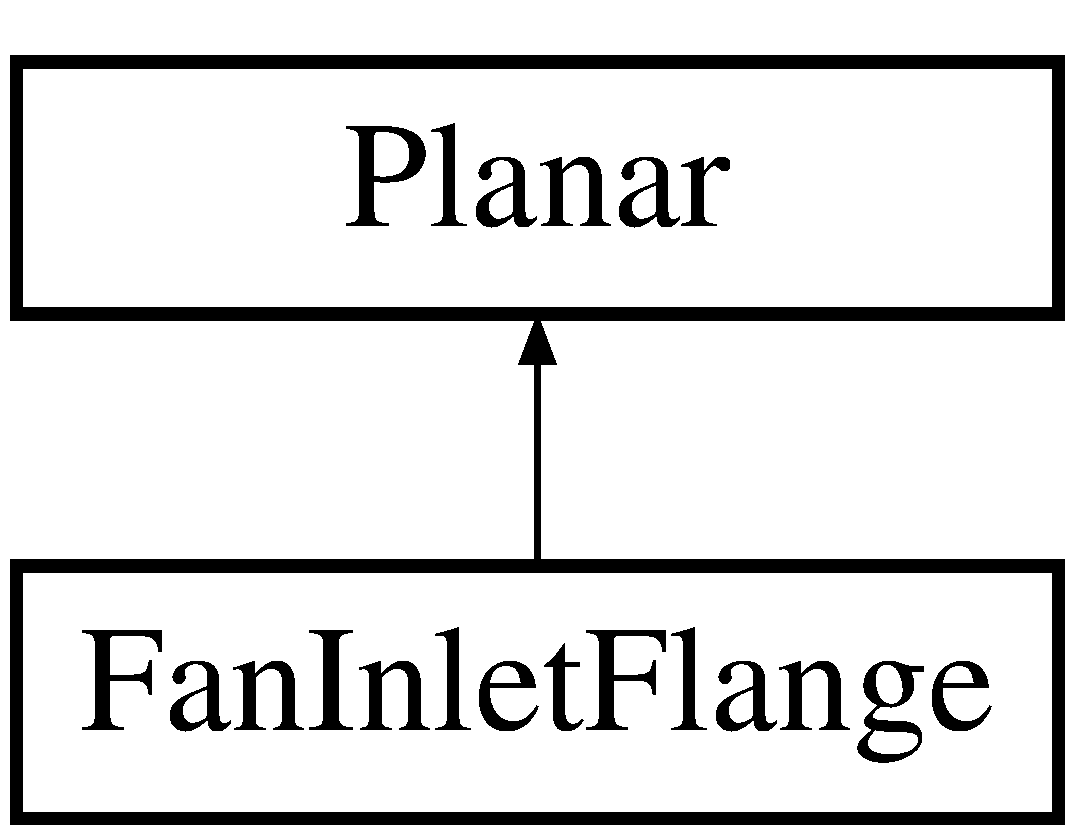
\includegraphics[height=2.000000cm]{d3/dca/class_fan_inlet_flange}
\end{center}
\end{figure}
\subsection*{Public Member Functions}
\begin{DoxyCompactItemize}
\item 
\mbox{\Hypertarget{class_fan_inlet_flange_a56cdb0d5f1095a700a5aca9a3e938d54}\label{class_fan_inlet_flange_a56cdb0d5f1095a700a5aca9a3e938d54}} 
{\bfseries Fan\+Inlet\+Flange} (double circular\+Duct\+Diameter, double tdx, double pbx)
\item 
\mbox{\Hypertarget{class_fan_inlet_flange_a1e584188ed5169268520c6a7d2e3fbf6}\label{class_fan_inlet_flange_a1e584188ed5169268520c6a7d2e3fbf6}} 
{\bfseries Fan\+Inlet\+Flange} (double rect\+Length, double rect\+Width, double tdx, double pbx)
\item 
\mbox{\Hypertarget{class_fan_inlet_flange_a40be4c42d0fa2670d90c1b24703346bd}\label{class_fan_inlet_flange_a40be4c42d0fa2670d90c1b24703346bd}} 
{\bfseries Fan\+Inlet\+Flange} (double rect\+Length, double rect\+Width, unsigned no\+Inlet\+Boxes, double tdx, double pbx)
\end{DoxyCompactItemize}
\subsection*{Additional Inherited Members}


\subsection{Detailed Description}


Definition at line 49 of file Planar.\+h.



The documentation for this class was generated from the following files\+:\begin{DoxyCompactItemize}
\item 
include/fans/Planar.\+h\item 
src/fans/Planar.\+cpp\end{DoxyCompactItemize}

\hypertarget{class_fan_or_evase_outlet_flange}{}\section{Fan\+Or\+Evase\+Outlet\+Flange Class Reference}
\label{class_fan_or_evase_outlet_flange}\index{Fan\+Or\+Evase\+Outlet\+Flange@{Fan\+Or\+Evase\+Outlet\+Flange}}
Inheritance diagram for Fan\+Or\+Evase\+Outlet\+Flange\+:\begin{figure}[H]
\begin{center}
\leavevmode
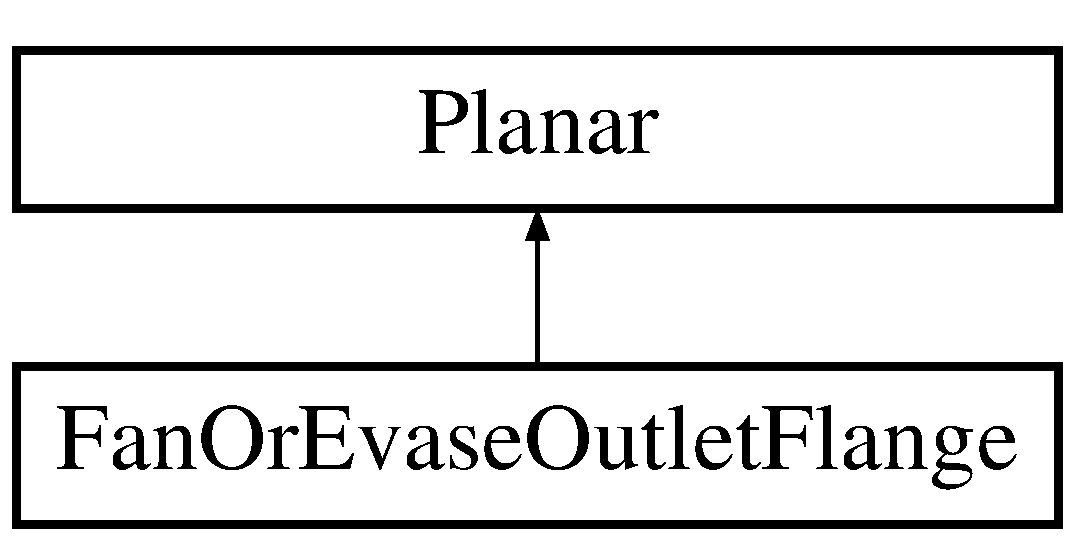
\includegraphics[height=2.000000cm]{d7/de3/class_fan_or_evase_outlet_flange}
\end{center}
\end{figure}
\subsection*{Public Member Functions}
\begin{DoxyCompactItemize}
\item 
\mbox{\Hypertarget{class_fan_or_evase_outlet_flange_aa5ffe09deb063462d9e1a08ce8ca3e79}\label{class_fan_or_evase_outlet_flange_aa5ffe09deb063462d9e1a08ce8ca3e79}} 
{\bfseries Fan\+Or\+Evase\+Outlet\+Flange} (double circular\+Duct\+Diameter, double tdx, double pbx)
\item 
\mbox{\Hypertarget{class_fan_or_evase_outlet_flange_a50a381091c3c22388a4c7af354444cb7}\label{class_fan_or_evase_outlet_flange_a50a381091c3c22388a4c7af354444cb7}} 
{\bfseries Fan\+Or\+Evase\+Outlet\+Flange} (double length, double width, double tdx, double pbx, unsigned no\+Inlet\+Boxes=1)
\end{DoxyCompactItemize}
\subsection*{Additional Inherited Members}


\subsection{Detailed Description}


Definition at line 43 of file Planar.\+h.



The documentation for this class was generated from the following files\+:\begin{DoxyCompactItemize}
\item 
include/fans/Planar.\+h\item 
src/fans/Planar.\+cpp\end{DoxyCompactItemize}

\hypertarget{class_fan_rated_info}{}\section{Fan\+Rated\+Info Class Reference}
\label{class_fan_rated_info}\index{Fan\+Rated\+Info@{Fan\+Rated\+Info}}
\subsection*{Public Member Functions}
\begin{DoxyCompactItemize}
\item 
\mbox{\Hypertarget{class_fan_rated_info_aa76c95537bd1a0cd0159a8d45df76f18}\label{class_fan_rated_info_aa76c95537bd1a0cd0159a8d45df76f18}} 
{\bfseries Fan\+Rated\+Info} (double const fan\+Speed, double const motor\+Speed, double const fan\+Speed\+Corrected, double const density\+Corrected, double const pressure\+Barometric\+Corrected)
\item 
\mbox{\Hypertarget{class_fan_rated_info_aa76c95537bd1a0cd0159a8d45df76f18}\label{class_fan_rated_info_aa76c95537bd1a0cd0159a8d45df76f18}} 
{\bfseries Fan\+Rated\+Info} (double const fan\+Speed, double const motor\+Speed, double const fan\+Speed\+Corrected, double const density\+Corrected, double const pressure\+Barometric\+Corrected)
\item 
\mbox{\Hypertarget{class_fan_rated_info_aa76c95537bd1a0cd0159a8d45df76f18}\label{class_fan_rated_info_aa76c95537bd1a0cd0159a8d45df76f18}} 
{\bfseries Fan\+Rated\+Info} (double const fan\+Speed, double const motor\+Speed, double const fan\+Speed\+Corrected, double const density\+Corrected, double const pressure\+Barometric\+Corrected)
\end{DoxyCompactItemize}
\subsection*{Friends}
\begin{DoxyCompactItemize}
\item 
\mbox{\Hypertarget{class_fan_rated_info_ad537df0087a4a6f474dc9d50579cc33d}\label{class_fan_rated_info_ad537df0087a4a6f474dc9d50579cc33d}} 
class {\bfseries Fan203}
\end{DoxyCompactItemize}


\subsection{Detailed Description}


Definition at line 6 of file Fan\+Shaft\+Power.\+h.



The documentation for this class was generated from the following file\+:\begin{DoxyCompactItemize}
\item 
\+\_\+\+C\+Pack\+\_\+\+Packages/\+Darwin/\+S\+T\+G\+Z/amo\+\_\+tools\+\_\+suite-\/-\/\+Darwin-\/x86\+\_\+64-\/\+Debug/amo\+\_\+tools\+\_\+suite/include/fans/Fan\+Shaft\+Power.\+h\end{DoxyCompactItemize}

\hypertarget{class_fan_shaft_power}{}\section{Fan\+Shaft\+Power Class Reference}
\label{class_fan_shaft_power}\index{Fan\+Shaft\+Power@{Fan\+Shaft\+Power}}
\subsection*{Public Member Functions}
\begin{DoxyCompactItemize}
\item 
\mbox{\Hypertarget{class_fan_shaft_power_a7ba1098a51b5f118ddbcc024e18a8e8b}\label{class_fan_shaft_power_a7ba1098a51b5f118ddbcc024e18a8e8b}} 
{\bfseries Fan\+Shaft\+Power} (bool fan\+Equipped\+With\+V\+FD, bool mains\+Voltage\+Data\+Available, double rated\+Hp, double synchronous\+Speed, double npv, double fla, double hi, double efficiency\+Motor, double efficiency\+V\+FD, double efficiency\+Belt, Fan\+Rated\+Info\+::\+Drive\+Type drive\+Type, double sum\+S\+EF)
\item 
\mbox{\Hypertarget{class_fan_shaft_power_a4c94a689955602eedd66046a3fcff730}\label{class_fan_shaft_power_a4c94a689955602eedd66046a3fcff730}} 
{\bfseries Fan\+Shaft\+Power} (bool fan\+Equipped\+With\+V\+FD, bool mains\+Voltage\+Data\+Available, double rated\+Hp, double synchronous\+Speed, double npv, double fla, double voltage, double amps, double power\+Factor\+At\+Load, double efficiency\+Motor, double efficiency\+V\+FD, double efficiency\+Belt, Fan\+Rated\+Info\+::\+Drive\+Type drive\+Type, double sum\+S\+EF)
\item 
\mbox{\Hypertarget{class_fan_shaft_power_a755745b0206e0a957168f6399a4ac438}\label{class_fan_shaft_power_a755745b0206e0a957168f6399a4ac438}} 
double {\bfseries get\+Fan\+Shaft\+Power} () const
\item 
\mbox{\Hypertarget{class_fan_shaft_power_a7a36d22c2301d3c634fc89e103daa148}\label{class_fan_shaft_power_a7a36d22c2301d3c634fc89e103daa148}} 
double {\bfseries get\+S\+EF} () const
\end{DoxyCompactItemize}


\subsection{Detailed Description}


Definition at line 22 of file Fan\+Shaft\+Power.\+h.



The documentation for this class was generated from the following files\+:\begin{DoxyCompactItemize}
\item 
include/fans/Fan\+Shaft\+Power.\+h\item 
src/fans/Fan\+Shaft\+Power.\+cpp\end{DoxyCompactItemize}

\hypertarget{class_field_data}{}\section{Field\+Data Class Reference}
\label{class_field_data}\index{Field\+Data@{Field\+Data}}


{\ttfamily \#include $<$Field\+Data.\+h$>$}

\subsection*{Public Types}
\begin{DoxyCompactItemize}
\item 
\mbox{\Hypertarget{class_field_data_a424e89914ba5684c01bb269dbe3312fd}\label{class_field_data_a424e89914ba5684c01bb269dbe3312fd}} 
enum \hyperlink{class_field_data_a424e89914ba5684c01bb269dbe3312fd}{Load\+Estimation\+Method} \{ \newline
{\bfseries P\+O\+W\+ER}, 
{\bfseries C\+U\+R\+R\+E\+NT}, 
{\bfseries P\+O\+W\+ER}, 
{\bfseries C\+U\+R\+R\+E\+NT}, 
\newline
{\bfseries P\+O\+W\+ER}, 
{\bfseries C\+U\+R\+R\+E\+NT}
 \}\begin{DoxyCompactList}\small\item\em Classifications of load estimation methods. \end{DoxyCompactList}
\item 
\mbox{\Hypertarget{class_field_data_a424e89914ba5684c01bb269dbe3312fd}\label{class_field_data_a424e89914ba5684c01bb269dbe3312fd}} 
enum \hyperlink{class_field_data_a424e89914ba5684c01bb269dbe3312fd}{Load\+Estimation\+Method} \{ \newline
{\bfseries P\+O\+W\+ER}, 
{\bfseries C\+U\+R\+R\+E\+NT}, 
{\bfseries P\+O\+W\+ER}, 
{\bfseries C\+U\+R\+R\+E\+NT}, 
\newline
{\bfseries P\+O\+W\+ER}, 
{\bfseries C\+U\+R\+R\+E\+NT}
 \}\begin{DoxyCompactList}\small\item\em Classifications of load estimation methods. \end{DoxyCompactList}
\item 
\mbox{\Hypertarget{class_field_data_a424e89914ba5684c01bb269dbe3312fd}\label{class_field_data_a424e89914ba5684c01bb269dbe3312fd}} 
enum \hyperlink{class_field_data_a424e89914ba5684c01bb269dbe3312fd}{Load\+Estimation\+Method} \{ \newline
{\bfseries P\+O\+W\+ER}, 
{\bfseries C\+U\+R\+R\+E\+NT}, 
{\bfseries P\+O\+W\+ER}, 
{\bfseries C\+U\+R\+R\+E\+NT}, 
\newline
{\bfseries P\+O\+W\+ER}, 
{\bfseries C\+U\+R\+R\+E\+NT}
 \}\begin{DoxyCompactList}\small\item\em Classifications of load estimation methods. \end{DoxyCompactList}
\end{DoxyCompactItemize}
\subsection*{Public Member Functions}
\begin{DoxyCompactItemize}
\item 
\hyperlink{class_field_data_a33158a88d05e657bd2c8007bae875454}{Field\+Data} (double flow\+Rate, double head, \hyperlink{class_field_data_a424e89914ba5684c01bb269dbe3312fd}{Load\+Estimation\+Method} load\+Estimation\+Method, double motor\+Power, double motor\+Amps, double voltage)
\item 
\hyperlink{class_field_data_a424e89914ba5684c01bb269dbe3312fd}{Load\+Estimation\+Method} \hyperlink{class_field_data_ae213fa76dd005d7fd251ef26beecd311}{get\+Load\+Estimation\+Method} () const
\item 
void \hyperlink{class_field_data_a7d1103b1832956d96146cbe26fb34a6d}{set\+Load\+Estimation\+Method} (\hyperlink{class_field_data_a424e89914ba5684c01bb269dbe3312fd}{Load\+Estimation\+Method} load\+Estimation\+Method)
\item 
double \hyperlink{class_field_data_a59b3261a5162b002d7b73a2d35561bd0}{get\+Flow\+Rate} () const
\item 
void \hyperlink{class_field_data_ad25c3e5a76b4e493e82d3f70cc3c0ed9}{set\+Flow\+Rate} (double flow\+Rate)
\item 
double \hyperlink{class_field_data_ac3e8e0b2de226c858b6c92cdb454bd0d}{get\+Head} () const
\item 
void \hyperlink{class_field_data_ac72a4f958930000bab0e2b772ee26711}{set\+Head} (double head)
\item 
double \hyperlink{class_field_data_a3e8e1bf84bbd00b9b52b803147968c81}{get\+Motor\+Power} () const
\item 
void \hyperlink{class_field_data_a078e6b4899e7046008ccc9de59bd0272}{set\+Motor\+Power} (double motor\+Power)
\item 
double \hyperlink{class_field_data_ad2b4fffb00fa7cfa6f69487e1034989a}{get\+Motor\+Amps} () const
\item 
void \hyperlink{class_field_data_a4f9373e8a215853b08bbe6a1915fb1a9}{set\+Motor\+Amps} (double motor\+Amps)
\item 
double \hyperlink{class_field_data_a1e8a55965e6cbd8c7b49c0dd5fbee002}{get\+Voltage} () const
\item 
void \hyperlink{class_field_data_a02735cc6956a3fce97bab645ef15dabc}{set\+Voltage} (double voltage)
\item 
\hyperlink{class_field_data_a33158a88d05e657bd2c8007bae875454}{Field\+Data} (double flow\+Rate, double head, \hyperlink{class_field_data_a424e89914ba5684c01bb269dbe3312fd}{Load\+Estimation\+Method} load\+Estimation\+Method, double motor\+Power, double motor\+Amps, double voltage)
\item 
\hyperlink{class_field_data_a424e89914ba5684c01bb269dbe3312fd}{Load\+Estimation\+Method} \hyperlink{class_field_data_ae213fa76dd005d7fd251ef26beecd311}{get\+Load\+Estimation\+Method} () const
\item 
void \hyperlink{class_field_data_a7d1103b1832956d96146cbe26fb34a6d}{set\+Load\+Estimation\+Method} (\hyperlink{class_field_data_a424e89914ba5684c01bb269dbe3312fd}{Load\+Estimation\+Method} load\+Estimation\+Method)
\item 
double \hyperlink{class_field_data_a59b3261a5162b002d7b73a2d35561bd0}{get\+Flow\+Rate} () const
\item 
void \hyperlink{class_field_data_ad25c3e5a76b4e493e82d3f70cc3c0ed9}{set\+Flow\+Rate} (double flow\+Rate)
\item 
double \hyperlink{class_field_data_ac3e8e0b2de226c858b6c92cdb454bd0d}{get\+Head} () const
\item 
void \hyperlink{class_field_data_ac72a4f958930000bab0e2b772ee26711}{set\+Head} (double head)
\item 
double \hyperlink{class_field_data_a3e8e1bf84bbd00b9b52b803147968c81}{get\+Motor\+Power} () const
\item 
void \hyperlink{class_field_data_a078e6b4899e7046008ccc9de59bd0272}{set\+Motor\+Power} (double motor\+Power)
\item 
double \hyperlink{class_field_data_ad2b4fffb00fa7cfa6f69487e1034989a}{get\+Motor\+Amps} () const
\item 
void \hyperlink{class_field_data_a4f9373e8a215853b08bbe6a1915fb1a9}{set\+Motor\+Amps} (double motor\+Amps)
\item 
double \hyperlink{class_field_data_a1e8a55965e6cbd8c7b49c0dd5fbee002}{get\+Voltage} () const
\item 
void \hyperlink{class_field_data_a02735cc6956a3fce97bab645ef15dabc}{set\+Voltage} (double voltage)
\item 
\hyperlink{class_field_data_a33158a88d05e657bd2c8007bae875454}{Field\+Data} (double flow\+Rate, double head, \hyperlink{class_field_data_a424e89914ba5684c01bb269dbe3312fd}{Load\+Estimation\+Method} load\+Estimation\+Method, double motor\+Power, double motor\+Amps, double voltage)
\item 
\hyperlink{class_field_data_a424e89914ba5684c01bb269dbe3312fd}{Load\+Estimation\+Method} \hyperlink{class_field_data_ae213fa76dd005d7fd251ef26beecd311}{get\+Load\+Estimation\+Method} () const
\item 
void \hyperlink{class_field_data_a7d1103b1832956d96146cbe26fb34a6d}{set\+Load\+Estimation\+Method} (\hyperlink{class_field_data_a424e89914ba5684c01bb269dbe3312fd}{Load\+Estimation\+Method} load\+Estimation\+Method)
\item 
double \hyperlink{class_field_data_a59b3261a5162b002d7b73a2d35561bd0}{get\+Flow\+Rate} () const
\item 
void \hyperlink{class_field_data_ad25c3e5a76b4e493e82d3f70cc3c0ed9}{set\+Flow\+Rate} (double flow\+Rate)
\item 
double \hyperlink{class_field_data_ac3e8e0b2de226c858b6c92cdb454bd0d}{get\+Head} () const
\item 
void \hyperlink{class_field_data_ac72a4f958930000bab0e2b772ee26711}{set\+Head} (double head)
\item 
double \hyperlink{class_field_data_a3e8e1bf84bbd00b9b52b803147968c81}{get\+Motor\+Power} () const
\item 
void \hyperlink{class_field_data_a078e6b4899e7046008ccc9de59bd0272}{set\+Motor\+Power} (double motor\+Power)
\item 
double \hyperlink{class_field_data_ad2b4fffb00fa7cfa6f69487e1034989a}{get\+Motor\+Amps} () const
\item 
void \hyperlink{class_field_data_a4f9373e8a215853b08bbe6a1915fb1a9}{set\+Motor\+Amps} (double motor\+Amps)
\item 
double \hyperlink{class_field_data_a1e8a55965e6cbd8c7b49c0dd5fbee002}{get\+Voltage} () const
\item 
void \hyperlink{class_field_data_a02735cc6956a3fce97bab645ef15dabc}{set\+Voltage} (double voltage)
\end{DoxyCompactItemize}


\subsection{Detailed Description}
Field Data class Contains all of the data that can be measured from a pump. 

Definition at line 21 of file Field\+Data.\+h.



\subsection{Constructor \& Destructor Documentation}
\mbox{\Hypertarget{class_field_data_a33158a88d05e657bd2c8007bae875454}\label{class_field_data_a33158a88d05e657bd2c8007bae875454}} 
\index{Field\+Data@{Field\+Data}!Field\+Data@{Field\+Data}}
\index{Field\+Data@{Field\+Data}!Field\+Data@{Field\+Data}}
\subsubsection{\texorpdfstring{Field\+Data()}{FieldData()}\hspace{0.1cm}{\footnotesize\ttfamily [1/3]}}
{\footnotesize\ttfamily Field\+Data\+::\+Field\+Data (\begin{DoxyParamCaption}\item[{double}]{flow\+Rate,  }\item[{double}]{head,  }\item[{\hyperlink{class_field_data_a424e89914ba5684c01bb269dbe3312fd}{Load\+Estimation\+Method}}]{load\+Estimation\+Method,  }\item[{double}]{motor\+Power,  }\item[{double}]{motor\+Amps,  }\item[{double}]{voltage }\end{DoxyParamCaption})\hspace{0.3cm}{\ttfamily [inline]}}

Constructor 
\begin{DoxyParams}{Parameters}
{\em flow\+Rate} & double, rate of flow. Units are gpm \\
\hline
{\em head} & double, pump head measured in feet \\
\hline
{\em load\+Estimation\+Method} & Load\+Estimation\+Method, classification of load estimation method \\
\hline
{\em motor\+Power} & double, power output of the pump\textquotesingle{}s motor in hp. \\
\hline
{\em motor\+Amps} & double, current measured from the pump\textquotesingle{}s motor in amps \\
\hline
{\em voltage} & double, the measured bus voltage in volts \\
\hline
\end{DoxyParams}
\begin{DoxyReturn}{Returns}
nothing 
\end{DoxyReturn}


Definition at line 41 of file Field\+Data.\+h.

\mbox{\Hypertarget{class_field_data_a33158a88d05e657bd2c8007bae875454}\label{class_field_data_a33158a88d05e657bd2c8007bae875454}} 
\index{Field\+Data@{Field\+Data}!Field\+Data@{Field\+Data}}
\index{Field\+Data@{Field\+Data}!Field\+Data@{Field\+Data}}
\subsubsection{\texorpdfstring{Field\+Data()}{FieldData()}\hspace{0.1cm}{\footnotesize\ttfamily [2/3]}}
{\footnotesize\ttfamily Field\+Data\+::\+Field\+Data (\begin{DoxyParamCaption}\item[{double}]{flow\+Rate,  }\item[{double}]{head,  }\item[{\hyperlink{class_field_data_a424e89914ba5684c01bb269dbe3312fd}{Load\+Estimation\+Method}}]{load\+Estimation\+Method,  }\item[{double}]{motor\+Power,  }\item[{double}]{motor\+Amps,  }\item[{double}]{voltage }\end{DoxyParamCaption})\hspace{0.3cm}{\ttfamily [inline]}}

Constructor 
\begin{DoxyParams}{Parameters}
{\em flow\+Rate} & double, rate of flow. Units are gpm \\
\hline
{\em head} & double, pump head measured in feet \\
\hline
{\em load\+Estimation\+Method} & Load\+Estimation\+Method, classification of load estimation method \\
\hline
{\em motor\+Power} & double, power output of the pump\textquotesingle{}s motor in hp. \\
\hline
{\em motor\+Amps} & double, current measured from the pump\textquotesingle{}s motor in amps \\
\hline
{\em voltage} & double, the measured bus voltage in volts \\
\hline
\end{DoxyParams}
\begin{DoxyReturn}{Returns}
nothing 
\end{DoxyReturn}


Definition at line 41 of file Field\+Data.\+h.

\mbox{\Hypertarget{class_field_data_a33158a88d05e657bd2c8007bae875454}\label{class_field_data_a33158a88d05e657bd2c8007bae875454}} 
\index{Field\+Data@{Field\+Data}!Field\+Data@{Field\+Data}}
\index{Field\+Data@{Field\+Data}!Field\+Data@{Field\+Data}}
\subsubsection{\texorpdfstring{Field\+Data()}{FieldData()}\hspace{0.1cm}{\footnotesize\ttfamily [3/3]}}
{\footnotesize\ttfamily Field\+Data\+::\+Field\+Data (\begin{DoxyParamCaption}\item[{double}]{flow\+Rate,  }\item[{double}]{head,  }\item[{\hyperlink{class_field_data_a424e89914ba5684c01bb269dbe3312fd}{Load\+Estimation\+Method}}]{load\+Estimation\+Method,  }\item[{double}]{motor\+Power,  }\item[{double}]{motor\+Amps,  }\item[{double}]{voltage }\end{DoxyParamCaption})\hspace{0.3cm}{\ttfamily [inline]}}

Constructor 
\begin{DoxyParams}{Parameters}
{\em flow\+Rate} & double, rate of flow. Units are gpm \\
\hline
{\em head} & double, pump head measured in feet \\
\hline
{\em load\+Estimation\+Method} & Load\+Estimation\+Method, classification of load estimation method \\
\hline
{\em motor\+Power} & double, power output of the pump\textquotesingle{}s motor in hp. \\
\hline
{\em motor\+Amps} & double, current measured from the pump\textquotesingle{}s motor in amps \\
\hline
{\em voltage} & double, the measured bus voltage in volts \\
\hline
\end{DoxyParams}
\begin{DoxyReturn}{Returns}
nothing 
\end{DoxyReturn}


Definition at line 41 of file Field\+Data.\+h.



\subsection{Member Function Documentation}
\mbox{\Hypertarget{class_field_data_a59b3261a5162b002d7b73a2d35561bd0}\label{class_field_data_a59b3261a5162b002d7b73a2d35561bd0}} 
\index{Field\+Data@{Field\+Data}!get\+Flow\+Rate@{get\+Flow\+Rate}}
\index{get\+Flow\+Rate@{get\+Flow\+Rate}!Field\+Data@{Field\+Data}}
\subsubsection{\texorpdfstring{get\+Flow\+Rate()}{getFlowRate()}\hspace{0.1cm}{\footnotesize\ttfamily [1/3]}}
{\footnotesize\ttfamily double Field\+Data\+::get\+Flow\+Rate (\begin{DoxyParamCaption}{ }\end{DoxyParamCaption}) const\hspace{0.3cm}{\ttfamily [inline]}}

Gets the rate of flow

\begin{DoxyReturn}{Returns}
double, rate of flow in gpm 
\end{DoxyReturn}


Definition at line 84 of file Field\+Data.\+h.

\mbox{\Hypertarget{class_field_data_a59b3261a5162b002d7b73a2d35561bd0}\label{class_field_data_a59b3261a5162b002d7b73a2d35561bd0}} 
\index{Field\+Data@{Field\+Data}!get\+Flow\+Rate@{get\+Flow\+Rate}}
\index{get\+Flow\+Rate@{get\+Flow\+Rate}!Field\+Data@{Field\+Data}}
\subsubsection{\texorpdfstring{get\+Flow\+Rate()}{getFlowRate()}\hspace{0.1cm}{\footnotesize\ttfamily [2/3]}}
{\footnotesize\ttfamily double Field\+Data\+::get\+Flow\+Rate (\begin{DoxyParamCaption}{ }\end{DoxyParamCaption}) const\hspace{0.3cm}{\ttfamily [inline]}}

Gets the rate of flow

\begin{DoxyReturn}{Returns}
double, rate of flow in gpm 
\end{DoxyReturn}


Definition at line 84 of file Field\+Data.\+h.

\mbox{\Hypertarget{class_field_data_a59b3261a5162b002d7b73a2d35561bd0}\label{class_field_data_a59b3261a5162b002d7b73a2d35561bd0}} 
\index{Field\+Data@{Field\+Data}!get\+Flow\+Rate@{get\+Flow\+Rate}}
\index{get\+Flow\+Rate@{get\+Flow\+Rate}!Field\+Data@{Field\+Data}}
\subsubsection{\texorpdfstring{get\+Flow\+Rate()}{getFlowRate()}\hspace{0.1cm}{\footnotesize\ttfamily [3/3]}}
{\footnotesize\ttfamily double Field\+Data\+::get\+Flow\+Rate (\begin{DoxyParamCaption}{ }\end{DoxyParamCaption}) const\hspace{0.3cm}{\ttfamily [inline]}}

Gets the rate of flow

\begin{DoxyReturn}{Returns}
double, rate of flow in gpm 
\end{DoxyReturn}


Definition at line 84 of file Field\+Data.\+h.

\mbox{\Hypertarget{class_field_data_ac3e8e0b2de226c858b6c92cdb454bd0d}\label{class_field_data_ac3e8e0b2de226c858b6c92cdb454bd0d}} 
\index{Field\+Data@{Field\+Data}!get\+Head@{get\+Head}}
\index{get\+Head@{get\+Head}!Field\+Data@{Field\+Data}}
\subsubsection{\texorpdfstring{get\+Head()}{getHead()}\hspace{0.1cm}{\footnotesize\ttfamily [1/3]}}
{\footnotesize\ttfamily double Field\+Data\+::get\+Head (\begin{DoxyParamCaption}{ }\end{DoxyParamCaption}) const\hspace{0.3cm}{\ttfamily [inline]}}

Gets the pump head

\begin{DoxyReturn}{Returns}
double, pump head in ft 
\end{DoxyReturn}


Definition at line 104 of file Field\+Data.\+h.

\mbox{\Hypertarget{class_field_data_ac3e8e0b2de226c858b6c92cdb454bd0d}\label{class_field_data_ac3e8e0b2de226c858b6c92cdb454bd0d}} 
\index{Field\+Data@{Field\+Data}!get\+Head@{get\+Head}}
\index{get\+Head@{get\+Head}!Field\+Data@{Field\+Data}}
\subsubsection{\texorpdfstring{get\+Head()}{getHead()}\hspace{0.1cm}{\footnotesize\ttfamily [2/3]}}
{\footnotesize\ttfamily double Field\+Data\+::get\+Head (\begin{DoxyParamCaption}{ }\end{DoxyParamCaption}) const\hspace{0.3cm}{\ttfamily [inline]}}

Gets the pump head

\begin{DoxyReturn}{Returns}
double, pump head in ft 
\end{DoxyReturn}


Definition at line 104 of file Field\+Data.\+h.

\mbox{\Hypertarget{class_field_data_ac3e8e0b2de226c858b6c92cdb454bd0d}\label{class_field_data_ac3e8e0b2de226c858b6c92cdb454bd0d}} 
\index{Field\+Data@{Field\+Data}!get\+Head@{get\+Head}}
\index{get\+Head@{get\+Head}!Field\+Data@{Field\+Data}}
\subsubsection{\texorpdfstring{get\+Head()}{getHead()}\hspace{0.1cm}{\footnotesize\ttfamily [3/3]}}
{\footnotesize\ttfamily double Field\+Data\+::get\+Head (\begin{DoxyParamCaption}{ }\end{DoxyParamCaption}) const\hspace{0.3cm}{\ttfamily [inline]}}

Gets the pump head

\begin{DoxyReturn}{Returns}
double, pump head in ft 
\end{DoxyReturn}


Definition at line 104 of file Field\+Data.\+h.

\mbox{\Hypertarget{class_field_data_ae213fa76dd005d7fd251ef26beecd311}\label{class_field_data_ae213fa76dd005d7fd251ef26beecd311}} 
\index{Field\+Data@{Field\+Data}!get\+Load\+Estimation\+Method@{get\+Load\+Estimation\+Method}}
\index{get\+Load\+Estimation\+Method@{get\+Load\+Estimation\+Method}!Field\+Data@{Field\+Data}}
\subsubsection{\texorpdfstring{get\+Load\+Estimation\+Method()}{getLoadEstimationMethod()}\hspace{0.1cm}{\footnotesize\ttfamily [1/3]}}
{\footnotesize\ttfamily \hyperlink{class_field_data_a424e89914ba5684c01bb269dbe3312fd}{Load\+Estimation\+Method} Field\+Data\+::get\+Load\+Estimation\+Method (\begin{DoxyParamCaption}{ }\end{DoxyParamCaption}) const\hspace{0.3cm}{\ttfamily [inline]}}

Gets the classification of the load estimation method

\begin{DoxyReturn}{Returns}
Load\+Estimation\+Method, classification of the load estimation method 
\end{DoxyReturn}


Definition at line 64 of file Field\+Data.\+h.

\mbox{\Hypertarget{class_field_data_ae213fa76dd005d7fd251ef26beecd311}\label{class_field_data_ae213fa76dd005d7fd251ef26beecd311}} 
\index{Field\+Data@{Field\+Data}!get\+Load\+Estimation\+Method@{get\+Load\+Estimation\+Method}}
\index{get\+Load\+Estimation\+Method@{get\+Load\+Estimation\+Method}!Field\+Data@{Field\+Data}}
\subsubsection{\texorpdfstring{get\+Load\+Estimation\+Method()}{getLoadEstimationMethod()}\hspace{0.1cm}{\footnotesize\ttfamily [2/3]}}
{\footnotesize\ttfamily \hyperlink{class_field_data_a424e89914ba5684c01bb269dbe3312fd}{Load\+Estimation\+Method} Field\+Data\+::get\+Load\+Estimation\+Method (\begin{DoxyParamCaption}{ }\end{DoxyParamCaption}) const\hspace{0.3cm}{\ttfamily [inline]}}

Gets the classification of the load estimation method

\begin{DoxyReturn}{Returns}
Load\+Estimation\+Method, classification of the load estimation method 
\end{DoxyReturn}


Definition at line 64 of file Field\+Data.\+h.

\mbox{\Hypertarget{class_field_data_ae213fa76dd005d7fd251ef26beecd311}\label{class_field_data_ae213fa76dd005d7fd251ef26beecd311}} 
\index{Field\+Data@{Field\+Data}!get\+Load\+Estimation\+Method@{get\+Load\+Estimation\+Method}}
\index{get\+Load\+Estimation\+Method@{get\+Load\+Estimation\+Method}!Field\+Data@{Field\+Data}}
\subsubsection{\texorpdfstring{get\+Load\+Estimation\+Method()}{getLoadEstimationMethod()}\hspace{0.1cm}{\footnotesize\ttfamily [3/3]}}
{\footnotesize\ttfamily \hyperlink{class_field_data_a424e89914ba5684c01bb269dbe3312fd}{Load\+Estimation\+Method} Field\+Data\+::get\+Load\+Estimation\+Method (\begin{DoxyParamCaption}{ }\end{DoxyParamCaption}) const\hspace{0.3cm}{\ttfamily [inline]}}

Gets the classification of the load estimation method

\begin{DoxyReturn}{Returns}
Load\+Estimation\+Method, classification of the load estimation method 
\end{DoxyReturn}


Definition at line 64 of file Field\+Data.\+h.

\mbox{\Hypertarget{class_field_data_ad2b4fffb00fa7cfa6f69487e1034989a}\label{class_field_data_ad2b4fffb00fa7cfa6f69487e1034989a}} 
\index{Field\+Data@{Field\+Data}!get\+Motor\+Amps@{get\+Motor\+Amps}}
\index{get\+Motor\+Amps@{get\+Motor\+Amps}!Field\+Data@{Field\+Data}}
\subsubsection{\texorpdfstring{get\+Motor\+Amps()}{getMotorAmps()}\hspace{0.1cm}{\footnotesize\ttfamily [1/3]}}
{\footnotesize\ttfamily double Field\+Data\+::get\+Motor\+Amps (\begin{DoxyParamCaption}{ }\end{DoxyParamCaption}) const\hspace{0.3cm}{\ttfamily [inline]}}

Gets the current measured from the pump\textquotesingle{}s motor

\begin{DoxyReturn}{Returns}
double, current measured from pump\textquotesingle{}s motor in amps 
\end{DoxyReturn}


Definition at line 144 of file Field\+Data.\+h.

\mbox{\Hypertarget{class_field_data_ad2b4fffb00fa7cfa6f69487e1034989a}\label{class_field_data_ad2b4fffb00fa7cfa6f69487e1034989a}} 
\index{Field\+Data@{Field\+Data}!get\+Motor\+Amps@{get\+Motor\+Amps}}
\index{get\+Motor\+Amps@{get\+Motor\+Amps}!Field\+Data@{Field\+Data}}
\subsubsection{\texorpdfstring{get\+Motor\+Amps()}{getMotorAmps()}\hspace{0.1cm}{\footnotesize\ttfamily [2/3]}}
{\footnotesize\ttfamily double Field\+Data\+::get\+Motor\+Amps (\begin{DoxyParamCaption}{ }\end{DoxyParamCaption}) const\hspace{0.3cm}{\ttfamily [inline]}}

Gets the current measured from the pump\textquotesingle{}s motor

\begin{DoxyReturn}{Returns}
double, current measured from pump\textquotesingle{}s motor in amps 
\end{DoxyReturn}


Definition at line 144 of file Field\+Data.\+h.

\mbox{\Hypertarget{class_field_data_ad2b4fffb00fa7cfa6f69487e1034989a}\label{class_field_data_ad2b4fffb00fa7cfa6f69487e1034989a}} 
\index{Field\+Data@{Field\+Data}!get\+Motor\+Amps@{get\+Motor\+Amps}}
\index{get\+Motor\+Amps@{get\+Motor\+Amps}!Field\+Data@{Field\+Data}}
\subsubsection{\texorpdfstring{get\+Motor\+Amps()}{getMotorAmps()}\hspace{0.1cm}{\footnotesize\ttfamily [3/3]}}
{\footnotesize\ttfamily double Field\+Data\+::get\+Motor\+Amps (\begin{DoxyParamCaption}{ }\end{DoxyParamCaption}) const\hspace{0.3cm}{\ttfamily [inline]}}

Gets the current measured from the pump\textquotesingle{}s motor

\begin{DoxyReturn}{Returns}
double, current measured from pump\textquotesingle{}s motor in amps 
\end{DoxyReturn}


Definition at line 144 of file Field\+Data.\+h.

\mbox{\Hypertarget{class_field_data_a3e8e1bf84bbd00b9b52b803147968c81}\label{class_field_data_a3e8e1bf84bbd00b9b52b803147968c81}} 
\index{Field\+Data@{Field\+Data}!get\+Motor\+Power@{get\+Motor\+Power}}
\index{get\+Motor\+Power@{get\+Motor\+Power}!Field\+Data@{Field\+Data}}
\subsubsection{\texorpdfstring{get\+Motor\+Power()}{getMotorPower()}\hspace{0.1cm}{\footnotesize\ttfamily [1/3]}}
{\footnotesize\ttfamily double Field\+Data\+::get\+Motor\+Power (\begin{DoxyParamCaption}{ }\end{DoxyParamCaption}) const\hspace{0.3cm}{\ttfamily [inline]}}

Gets the power output of the pump\textquotesingle{}s motor

\begin{DoxyReturn}{Returns}
double, pump motor\textquotesingle{}s output power in hp 
\end{DoxyReturn}


Definition at line 124 of file Field\+Data.\+h.

\mbox{\Hypertarget{class_field_data_a3e8e1bf84bbd00b9b52b803147968c81}\label{class_field_data_a3e8e1bf84bbd00b9b52b803147968c81}} 
\index{Field\+Data@{Field\+Data}!get\+Motor\+Power@{get\+Motor\+Power}}
\index{get\+Motor\+Power@{get\+Motor\+Power}!Field\+Data@{Field\+Data}}
\subsubsection{\texorpdfstring{get\+Motor\+Power()}{getMotorPower()}\hspace{0.1cm}{\footnotesize\ttfamily [2/3]}}
{\footnotesize\ttfamily double Field\+Data\+::get\+Motor\+Power (\begin{DoxyParamCaption}{ }\end{DoxyParamCaption}) const\hspace{0.3cm}{\ttfamily [inline]}}

Gets the power output of the pump\textquotesingle{}s motor

\begin{DoxyReturn}{Returns}
double, pump motor\textquotesingle{}s output power in hp 
\end{DoxyReturn}


Definition at line 124 of file Field\+Data.\+h.

\mbox{\Hypertarget{class_field_data_a3e8e1bf84bbd00b9b52b803147968c81}\label{class_field_data_a3e8e1bf84bbd00b9b52b803147968c81}} 
\index{Field\+Data@{Field\+Data}!get\+Motor\+Power@{get\+Motor\+Power}}
\index{get\+Motor\+Power@{get\+Motor\+Power}!Field\+Data@{Field\+Data}}
\subsubsection{\texorpdfstring{get\+Motor\+Power()}{getMotorPower()}\hspace{0.1cm}{\footnotesize\ttfamily [3/3]}}
{\footnotesize\ttfamily double Field\+Data\+::get\+Motor\+Power (\begin{DoxyParamCaption}{ }\end{DoxyParamCaption}) const\hspace{0.3cm}{\ttfamily [inline]}}

Gets the power output of the pump\textquotesingle{}s motor

\begin{DoxyReturn}{Returns}
double, pump motor\textquotesingle{}s output power in hp 
\end{DoxyReturn}


Definition at line 124 of file Field\+Data.\+h.

\mbox{\Hypertarget{class_field_data_a1e8a55965e6cbd8c7b49c0dd5fbee002}\label{class_field_data_a1e8a55965e6cbd8c7b49c0dd5fbee002}} 
\index{Field\+Data@{Field\+Data}!get\+Voltage@{get\+Voltage}}
\index{get\+Voltage@{get\+Voltage}!Field\+Data@{Field\+Data}}
\subsubsection{\texorpdfstring{get\+Voltage()}{getVoltage()}\hspace{0.1cm}{\footnotesize\ttfamily [1/3]}}
{\footnotesize\ttfamily double Field\+Data\+::get\+Voltage (\begin{DoxyParamCaption}{ }\end{DoxyParamCaption}) const\hspace{0.3cm}{\ttfamily [inline]}}

Gets the measured bus voltage

\begin{DoxyReturn}{Returns}
double, measured bus voltage in volts 
\end{DoxyReturn}


Definition at line 164 of file Field\+Data.\+h.

\mbox{\Hypertarget{class_field_data_a1e8a55965e6cbd8c7b49c0dd5fbee002}\label{class_field_data_a1e8a55965e6cbd8c7b49c0dd5fbee002}} 
\index{Field\+Data@{Field\+Data}!get\+Voltage@{get\+Voltage}}
\index{get\+Voltage@{get\+Voltage}!Field\+Data@{Field\+Data}}
\subsubsection{\texorpdfstring{get\+Voltage()}{getVoltage()}\hspace{0.1cm}{\footnotesize\ttfamily [2/3]}}
{\footnotesize\ttfamily double Field\+Data\+::get\+Voltage (\begin{DoxyParamCaption}{ }\end{DoxyParamCaption}) const\hspace{0.3cm}{\ttfamily [inline]}}

Gets the measured bus voltage

\begin{DoxyReturn}{Returns}
double, measured bus voltage in volts 
\end{DoxyReturn}


Definition at line 164 of file Field\+Data.\+h.

\mbox{\Hypertarget{class_field_data_a1e8a55965e6cbd8c7b49c0dd5fbee002}\label{class_field_data_a1e8a55965e6cbd8c7b49c0dd5fbee002}} 
\index{Field\+Data@{Field\+Data}!get\+Voltage@{get\+Voltage}}
\index{get\+Voltage@{get\+Voltage}!Field\+Data@{Field\+Data}}
\subsubsection{\texorpdfstring{get\+Voltage()}{getVoltage()}\hspace{0.1cm}{\footnotesize\ttfamily [3/3]}}
{\footnotesize\ttfamily double Field\+Data\+::get\+Voltage (\begin{DoxyParamCaption}{ }\end{DoxyParamCaption}) const\hspace{0.3cm}{\ttfamily [inline]}}

Gets the measured bus voltage

\begin{DoxyReturn}{Returns}
double, measured bus voltage in volts 
\end{DoxyReturn}


Definition at line 164 of file Field\+Data.\+h.

\mbox{\Hypertarget{class_field_data_ad25c3e5a76b4e493e82d3f70cc3c0ed9}\label{class_field_data_ad25c3e5a76b4e493e82d3f70cc3c0ed9}} 
\index{Field\+Data@{Field\+Data}!set\+Flow\+Rate@{set\+Flow\+Rate}}
\index{set\+Flow\+Rate@{set\+Flow\+Rate}!Field\+Data@{Field\+Data}}
\subsubsection{\texorpdfstring{set\+Flow\+Rate()}{setFlowRate()}\hspace{0.1cm}{\footnotesize\ttfamily [1/3]}}
{\footnotesize\ttfamily void Field\+Data\+::set\+Flow\+Rate (\begin{DoxyParamCaption}\item[{double}]{flow\+Rate }\end{DoxyParamCaption})\hspace{0.3cm}{\ttfamily [inline]}}

Sets the rate of flow


\begin{DoxyParams}{Parameters}
{\em flow\+Rate} & double, rate of flow in gpm\\
\hline
\end{DoxyParams}
\begin{DoxyReturn}{Returns}
nothing 
\end{DoxyReturn}


Definition at line 95 of file Field\+Data.\+h.

\mbox{\Hypertarget{class_field_data_ad25c3e5a76b4e493e82d3f70cc3c0ed9}\label{class_field_data_ad25c3e5a76b4e493e82d3f70cc3c0ed9}} 
\index{Field\+Data@{Field\+Data}!set\+Flow\+Rate@{set\+Flow\+Rate}}
\index{set\+Flow\+Rate@{set\+Flow\+Rate}!Field\+Data@{Field\+Data}}
\subsubsection{\texorpdfstring{set\+Flow\+Rate()}{setFlowRate()}\hspace{0.1cm}{\footnotesize\ttfamily [2/3]}}
{\footnotesize\ttfamily void Field\+Data\+::set\+Flow\+Rate (\begin{DoxyParamCaption}\item[{double}]{flow\+Rate }\end{DoxyParamCaption})\hspace{0.3cm}{\ttfamily [inline]}}

Sets the rate of flow


\begin{DoxyParams}{Parameters}
{\em flow\+Rate} & double, rate of flow in gpm\\
\hline
\end{DoxyParams}
\begin{DoxyReturn}{Returns}
nothing 
\end{DoxyReturn}


Definition at line 95 of file Field\+Data.\+h.

\mbox{\Hypertarget{class_field_data_ad25c3e5a76b4e493e82d3f70cc3c0ed9}\label{class_field_data_ad25c3e5a76b4e493e82d3f70cc3c0ed9}} 
\index{Field\+Data@{Field\+Data}!set\+Flow\+Rate@{set\+Flow\+Rate}}
\index{set\+Flow\+Rate@{set\+Flow\+Rate}!Field\+Data@{Field\+Data}}
\subsubsection{\texorpdfstring{set\+Flow\+Rate()}{setFlowRate()}\hspace{0.1cm}{\footnotesize\ttfamily [3/3]}}
{\footnotesize\ttfamily void Field\+Data\+::set\+Flow\+Rate (\begin{DoxyParamCaption}\item[{double}]{flow\+Rate }\end{DoxyParamCaption})\hspace{0.3cm}{\ttfamily [inline]}}

Sets the rate of flow


\begin{DoxyParams}{Parameters}
{\em flow\+Rate} & double, rate of flow in gpm\\
\hline
\end{DoxyParams}
\begin{DoxyReturn}{Returns}
nothing 
\end{DoxyReturn}


Definition at line 95 of file Field\+Data.\+h.

\mbox{\Hypertarget{class_field_data_ac72a4f958930000bab0e2b772ee26711}\label{class_field_data_ac72a4f958930000bab0e2b772ee26711}} 
\index{Field\+Data@{Field\+Data}!set\+Head@{set\+Head}}
\index{set\+Head@{set\+Head}!Field\+Data@{Field\+Data}}
\subsubsection{\texorpdfstring{set\+Head()}{setHead()}\hspace{0.1cm}{\footnotesize\ttfamily [1/3]}}
{\footnotesize\ttfamily void Field\+Data\+::set\+Head (\begin{DoxyParamCaption}\item[{double}]{head }\end{DoxyParamCaption})\hspace{0.3cm}{\ttfamily [inline]}}

Sets the pump head


\begin{DoxyParams}{Parameters}
{\em head} & double, pump head in ft\\
\hline
\end{DoxyParams}
\begin{DoxyReturn}{Returns}
nothing 
\end{DoxyReturn}


Definition at line 115 of file Field\+Data.\+h.

\mbox{\Hypertarget{class_field_data_ac72a4f958930000bab0e2b772ee26711}\label{class_field_data_ac72a4f958930000bab0e2b772ee26711}} 
\index{Field\+Data@{Field\+Data}!set\+Head@{set\+Head}}
\index{set\+Head@{set\+Head}!Field\+Data@{Field\+Data}}
\subsubsection{\texorpdfstring{set\+Head()}{setHead()}\hspace{0.1cm}{\footnotesize\ttfamily [2/3]}}
{\footnotesize\ttfamily void Field\+Data\+::set\+Head (\begin{DoxyParamCaption}\item[{double}]{head }\end{DoxyParamCaption})\hspace{0.3cm}{\ttfamily [inline]}}

Sets the pump head


\begin{DoxyParams}{Parameters}
{\em head} & double, pump head in ft\\
\hline
\end{DoxyParams}
\begin{DoxyReturn}{Returns}
nothing 
\end{DoxyReturn}


Definition at line 115 of file Field\+Data.\+h.

\mbox{\Hypertarget{class_field_data_ac72a4f958930000bab0e2b772ee26711}\label{class_field_data_ac72a4f958930000bab0e2b772ee26711}} 
\index{Field\+Data@{Field\+Data}!set\+Head@{set\+Head}}
\index{set\+Head@{set\+Head}!Field\+Data@{Field\+Data}}
\subsubsection{\texorpdfstring{set\+Head()}{setHead()}\hspace{0.1cm}{\footnotesize\ttfamily [3/3]}}
{\footnotesize\ttfamily void Field\+Data\+::set\+Head (\begin{DoxyParamCaption}\item[{double}]{head }\end{DoxyParamCaption})\hspace{0.3cm}{\ttfamily [inline]}}

Sets the pump head


\begin{DoxyParams}{Parameters}
{\em head} & double, pump head in ft\\
\hline
\end{DoxyParams}
\begin{DoxyReturn}{Returns}
nothing 
\end{DoxyReturn}


Definition at line 115 of file Field\+Data.\+h.

\mbox{\Hypertarget{class_field_data_a7d1103b1832956d96146cbe26fb34a6d}\label{class_field_data_a7d1103b1832956d96146cbe26fb34a6d}} 
\index{Field\+Data@{Field\+Data}!set\+Load\+Estimation\+Method@{set\+Load\+Estimation\+Method}}
\index{set\+Load\+Estimation\+Method@{set\+Load\+Estimation\+Method}!Field\+Data@{Field\+Data}}
\subsubsection{\texorpdfstring{set\+Load\+Estimation\+Method()}{setLoadEstimationMethod()}\hspace{0.1cm}{\footnotesize\ttfamily [1/3]}}
{\footnotesize\ttfamily void Field\+Data\+::set\+Load\+Estimation\+Method (\begin{DoxyParamCaption}\item[{\hyperlink{class_field_data_a424e89914ba5684c01bb269dbe3312fd}{Load\+Estimation\+Method}}]{load\+Estimation\+Method }\end{DoxyParamCaption})\hspace{0.3cm}{\ttfamily [inline]}}

Sets the classification of the load estimation method


\begin{DoxyParams}{Parameters}
{\em load\+Estimation\+Method} & Load\+Estimation\+Method, classification of the load estimation method\\
\hline
\end{DoxyParams}
\begin{DoxyReturn}{Returns}
nothing 
\end{DoxyReturn}


Definition at line 75 of file Field\+Data.\+h.

\mbox{\Hypertarget{class_field_data_a7d1103b1832956d96146cbe26fb34a6d}\label{class_field_data_a7d1103b1832956d96146cbe26fb34a6d}} 
\index{Field\+Data@{Field\+Data}!set\+Load\+Estimation\+Method@{set\+Load\+Estimation\+Method}}
\index{set\+Load\+Estimation\+Method@{set\+Load\+Estimation\+Method}!Field\+Data@{Field\+Data}}
\subsubsection{\texorpdfstring{set\+Load\+Estimation\+Method()}{setLoadEstimationMethod()}\hspace{0.1cm}{\footnotesize\ttfamily [2/3]}}
{\footnotesize\ttfamily void Field\+Data\+::set\+Load\+Estimation\+Method (\begin{DoxyParamCaption}\item[{\hyperlink{class_field_data_a424e89914ba5684c01bb269dbe3312fd}{Load\+Estimation\+Method}}]{load\+Estimation\+Method }\end{DoxyParamCaption})\hspace{0.3cm}{\ttfamily [inline]}}

Sets the classification of the load estimation method


\begin{DoxyParams}{Parameters}
{\em load\+Estimation\+Method} & Load\+Estimation\+Method, classification of the load estimation method\\
\hline
\end{DoxyParams}
\begin{DoxyReturn}{Returns}
nothing 
\end{DoxyReturn}


Definition at line 75 of file Field\+Data.\+h.

\mbox{\Hypertarget{class_field_data_a7d1103b1832956d96146cbe26fb34a6d}\label{class_field_data_a7d1103b1832956d96146cbe26fb34a6d}} 
\index{Field\+Data@{Field\+Data}!set\+Load\+Estimation\+Method@{set\+Load\+Estimation\+Method}}
\index{set\+Load\+Estimation\+Method@{set\+Load\+Estimation\+Method}!Field\+Data@{Field\+Data}}
\subsubsection{\texorpdfstring{set\+Load\+Estimation\+Method()}{setLoadEstimationMethod()}\hspace{0.1cm}{\footnotesize\ttfamily [3/3]}}
{\footnotesize\ttfamily void Field\+Data\+::set\+Load\+Estimation\+Method (\begin{DoxyParamCaption}\item[{\hyperlink{class_field_data_a424e89914ba5684c01bb269dbe3312fd}{Load\+Estimation\+Method}}]{load\+Estimation\+Method }\end{DoxyParamCaption})\hspace{0.3cm}{\ttfamily [inline]}}

Sets the classification of the load estimation method


\begin{DoxyParams}{Parameters}
{\em load\+Estimation\+Method} & Load\+Estimation\+Method, classification of the load estimation method\\
\hline
\end{DoxyParams}
\begin{DoxyReturn}{Returns}
nothing 
\end{DoxyReturn}


Definition at line 75 of file Field\+Data.\+h.

\mbox{\Hypertarget{class_field_data_a4f9373e8a215853b08bbe6a1915fb1a9}\label{class_field_data_a4f9373e8a215853b08bbe6a1915fb1a9}} 
\index{Field\+Data@{Field\+Data}!set\+Motor\+Amps@{set\+Motor\+Amps}}
\index{set\+Motor\+Amps@{set\+Motor\+Amps}!Field\+Data@{Field\+Data}}
\subsubsection{\texorpdfstring{set\+Motor\+Amps()}{setMotorAmps()}\hspace{0.1cm}{\footnotesize\ttfamily [1/3]}}
{\footnotesize\ttfamily void Field\+Data\+::set\+Motor\+Amps (\begin{DoxyParamCaption}\item[{double}]{motor\+Amps }\end{DoxyParamCaption})\hspace{0.3cm}{\ttfamily [inline]}}

Sets the current measured from the pump\textquotesingle{}s motor


\begin{DoxyParams}{Parameters}
{\em motor\+Amps} & double, current measured from pump\textquotesingle{}s motor in amps\\
\hline
\end{DoxyParams}
\begin{DoxyReturn}{Returns}
nothing 
\end{DoxyReturn}


Definition at line 155 of file Field\+Data.\+h.

\mbox{\Hypertarget{class_field_data_a4f9373e8a215853b08bbe6a1915fb1a9}\label{class_field_data_a4f9373e8a215853b08bbe6a1915fb1a9}} 
\index{Field\+Data@{Field\+Data}!set\+Motor\+Amps@{set\+Motor\+Amps}}
\index{set\+Motor\+Amps@{set\+Motor\+Amps}!Field\+Data@{Field\+Data}}
\subsubsection{\texorpdfstring{set\+Motor\+Amps()}{setMotorAmps()}\hspace{0.1cm}{\footnotesize\ttfamily [2/3]}}
{\footnotesize\ttfamily void Field\+Data\+::set\+Motor\+Amps (\begin{DoxyParamCaption}\item[{double}]{motor\+Amps }\end{DoxyParamCaption})\hspace{0.3cm}{\ttfamily [inline]}}

Sets the current measured from the pump\textquotesingle{}s motor


\begin{DoxyParams}{Parameters}
{\em motor\+Amps} & double, current measured from pump\textquotesingle{}s motor in amps\\
\hline
\end{DoxyParams}
\begin{DoxyReturn}{Returns}
nothing 
\end{DoxyReturn}


Definition at line 155 of file Field\+Data.\+h.

\mbox{\Hypertarget{class_field_data_a4f9373e8a215853b08bbe6a1915fb1a9}\label{class_field_data_a4f9373e8a215853b08bbe6a1915fb1a9}} 
\index{Field\+Data@{Field\+Data}!set\+Motor\+Amps@{set\+Motor\+Amps}}
\index{set\+Motor\+Amps@{set\+Motor\+Amps}!Field\+Data@{Field\+Data}}
\subsubsection{\texorpdfstring{set\+Motor\+Amps()}{setMotorAmps()}\hspace{0.1cm}{\footnotesize\ttfamily [3/3]}}
{\footnotesize\ttfamily void Field\+Data\+::set\+Motor\+Amps (\begin{DoxyParamCaption}\item[{double}]{motor\+Amps }\end{DoxyParamCaption})\hspace{0.3cm}{\ttfamily [inline]}}

Sets the current measured from the pump\textquotesingle{}s motor


\begin{DoxyParams}{Parameters}
{\em motor\+Amps} & double, current measured from pump\textquotesingle{}s motor in amps\\
\hline
\end{DoxyParams}
\begin{DoxyReturn}{Returns}
nothing 
\end{DoxyReturn}


Definition at line 155 of file Field\+Data.\+h.

\mbox{\Hypertarget{class_field_data_a078e6b4899e7046008ccc9de59bd0272}\label{class_field_data_a078e6b4899e7046008ccc9de59bd0272}} 
\index{Field\+Data@{Field\+Data}!set\+Motor\+Power@{set\+Motor\+Power}}
\index{set\+Motor\+Power@{set\+Motor\+Power}!Field\+Data@{Field\+Data}}
\subsubsection{\texorpdfstring{set\+Motor\+Power()}{setMotorPower()}\hspace{0.1cm}{\footnotesize\ttfamily [1/3]}}
{\footnotesize\ttfamily void Field\+Data\+::set\+Motor\+Power (\begin{DoxyParamCaption}\item[{double}]{motor\+Power }\end{DoxyParamCaption})\hspace{0.3cm}{\ttfamily [inline]}}

Sets the power output of the pump\textquotesingle{}s motor


\begin{DoxyParams}{Parameters}
{\em motor\+Power} & double, pump motor\textquotesingle{}s output power in hp\\
\hline
\end{DoxyParams}
\begin{DoxyReturn}{Returns}
nothing 
\end{DoxyReturn}


Definition at line 135 of file Field\+Data.\+h.

\mbox{\Hypertarget{class_field_data_a078e6b4899e7046008ccc9de59bd0272}\label{class_field_data_a078e6b4899e7046008ccc9de59bd0272}} 
\index{Field\+Data@{Field\+Data}!set\+Motor\+Power@{set\+Motor\+Power}}
\index{set\+Motor\+Power@{set\+Motor\+Power}!Field\+Data@{Field\+Data}}
\subsubsection{\texorpdfstring{set\+Motor\+Power()}{setMotorPower()}\hspace{0.1cm}{\footnotesize\ttfamily [2/3]}}
{\footnotesize\ttfamily void Field\+Data\+::set\+Motor\+Power (\begin{DoxyParamCaption}\item[{double}]{motor\+Power }\end{DoxyParamCaption})\hspace{0.3cm}{\ttfamily [inline]}}

Sets the power output of the pump\textquotesingle{}s motor


\begin{DoxyParams}{Parameters}
{\em motor\+Power} & double, pump motor\textquotesingle{}s output power in hp\\
\hline
\end{DoxyParams}
\begin{DoxyReturn}{Returns}
nothing 
\end{DoxyReturn}


Definition at line 135 of file Field\+Data.\+h.

\mbox{\Hypertarget{class_field_data_a078e6b4899e7046008ccc9de59bd0272}\label{class_field_data_a078e6b4899e7046008ccc9de59bd0272}} 
\index{Field\+Data@{Field\+Data}!set\+Motor\+Power@{set\+Motor\+Power}}
\index{set\+Motor\+Power@{set\+Motor\+Power}!Field\+Data@{Field\+Data}}
\subsubsection{\texorpdfstring{set\+Motor\+Power()}{setMotorPower()}\hspace{0.1cm}{\footnotesize\ttfamily [3/3]}}
{\footnotesize\ttfamily void Field\+Data\+::set\+Motor\+Power (\begin{DoxyParamCaption}\item[{double}]{motor\+Power }\end{DoxyParamCaption})\hspace{0.3cm}{\ttfamily [inline]}}

Sets the power output of the pump\textquotesingle{}s motor


\begin{DoxyParams}{Parameters}
{\em motor\+Power} & double, pump motor\textquotesingle{}s output power in hp\\
\hline
\end{DoxyParams}
\begin{DoxyReturn}{Returns}
nothing 
\end{DoxyReturn}


Definition at line 135 of file Field\+Data.\+h.

\mbox{\Hypertarget{class_field_data_a02735cc6956a3fce97bab645ef15dabc}\label{class_field_data_a02735cc6956a3fce97bab645ef15dabc}} 
\index{Field\+Data@{Field\+Data}!set\+Voltage@{set\+Voltage}}
\index{set\+Voltage@{set\+Voltage}!Field\+Data@{Field\+Data}}
\subsubsection{\texorpdfstring{set\+Voltage()}{setVoltage()}\hspace{0.1cm}{\footnotesize\ttfamily [1/3]}}
{\footnotesize\ttfamily void Field\+Data\+::set\+Voltage (\begin{DoxyParamCaption}\item[{double}]{voltage }\end{DoxyParamCaption})\hspace{0.3cm}{\ttfamily [inline]}}

Sets the measured bus voltage


\begin{DoxyParams}{Parameters}
{\em voltage} & double, measured bus voltage in volts\\
\hline
\end{DoxyParams}
\begin{DoxyReturn}{Returns}
nothing 
\end{DoxyReturn}


Definition at line 175 of file Field\+Data.\+h.

\mbox{\Hypertarget{class_field_data_a02735cc6956a3fce97bab645ef15dabc}\label{class_field_data_a02735cc6956a3fce97bab645ef15dabc}} 
\index{Field\+Data@{Field\+Data}!set\+Voltage@{set\+Voltage}}
\index{set\+Voltage@{set\+Voltage}!Field\+Data@{Field\+Data}}
\subsubsection{\texorpdfstring{set\+Voltage()}{setVoltage()}\hspace{0.1cm}{\footnotesize\ttfamily [2/3]}}
{\footnotesize\ttfamily void Field\+Data\+::set\+Voltage (\begin{DoxyParamCaption}\item[{double}]{voltage }\end{DoxyParamCaption})\hspace{0.3cm}{\ttfamily [inline]}}

Sets the measured bus voltage


\begin{DoxyParams}{Parameters}
{\em voltage} & double, measured bus voltage in volts\\
\hline
\end{DoxyParams}
\begin{DoxyReturn}{Returns}
nothing 
\end{DoxyReturn}


Definition at line 175 of file Field\+Data.\+h.

\mbox{\Hypertarget{class_field_data_a02735cc6956a3fce97bab645ef15dabc}\label{class_field_data_a02735cc6956a3fce97bab645ef15dabc}} 
\index{Field\+Data@{Field\+Data}!set\+Voltage@{set\+Voltage}}
\index{set\+Voltage@{set\+Voltage}!Field\+Data@{Field\+Data}}
\subsubsection{\texorpdfstring{set\+Voltage()}{setVoltage()}\hspace{0.1cm}{\footnotesize\ttfamily [3/3]}}
{\footnotesize\ttfamily void Field\+Data\+::set\+Voltage (\begin{DoxyParamCaption}\item[{double}]{voltage }\end{DoxyParamCaption})\hspace{0.3cm}{\ttfamily [inline]}}

Sets the measured bus voltage


\begin{DoxyParams}{Parameters}
{\em voltage} & double, measured bus voltage in volts\\
\hline
\end{DoxyParams}
\begin{DoxyReturn}{Returns}
nothing 
\end{DoxyReturn}


Definition at line 175 of file Field\+Data.\+h.



The documentation for this class was generated from the following file\+:\begin{DoxyCompactItemize}
\item 
\+\_\+\+C\+Pack\+\_\+\+Packages/\+Darwin/\+S\+T\+G\+Z/amo\+\_\+tools\+\_\+suite-\/-\/\+Darwin-\/x86\+\_\+64/amo\+\_\+tools\+\_\+suite/include/psat/\hyperlink{___c_pack___packages_2_darwin_2_s_t_g_z_2amo__tools__suite--_darwin-x86__64_2amo__tools__suite_2include_2psat_2_field_data_8h}{Field\+Data.\+h}\end{DoxyCompactItemize}

\hypertarget{class_financial}{}\section{Financial Class Reference}
\label{class_financial}\index{Financial@{Financial}}


{\ttfamily \#include $<$Financial.\+h$>$}

\subsection*{Public Member Functions}
\begin{DoxyCompactItemize}
\item 
\hyperlink{class_financial_abe8c4d82e9aede125e7e42ad3d53f90a}{Financial} (double operating\+Fraction, double unit\+Cost)
\item 
double \hyperlink{class_financial_a650ee2678b49d8d19b541f15d5a37c05}{get\+Operating\+Fraction} () const
\item 
void \hyperlink{class_financial_a966250111b2f7a00d797a9d153ee8a83}{set\+Operating\+Fraction} (double operating\+Fraction)
\item 
double \hyperlink{class_financial_adc3092e8f4cfd065042638236d21eaf4}{get\+Unit\+Cost} () const
\item 
void \hyperlink{class_financial_a84ead2ef72b2d348e05eb308d01e9265}{set\+Unit\+Cost} (double unit\+Cost)
\end{DoxyCompactItemize}


\subsection{Detailed Description}
\hyperlink{class_financial}{Financial} class Contains the properties relating to the cost of operating equipment. 

Definition at line 22 of file Financial.\+h.



\subsection{Constructor \& Destructor Documentation}
\mbox{\Hypertarget{class_financial_abe8c4d82e9aede125e7e42ad3d53f90a}\label{class_financial_abe8c4d82e9aede125e7e42ad3d53f90a}} 
\index{Financial@{Financial}!Financial@{Financial}}
\index{Financial@{Financial}!Financial@{Financial}}
\subsubsection{\texorpdfstring{Financial()}{Financial()}}
{\footnotesize\ttfamily Financial\+::\+Financial (\begin{DoxyParamCaption}\item[{double}]{operating\+Fraction,  }\item[{double}]{unit\+Cost }\end{DoxyParamCaption})\hspace{0.3cm}{\ttfamily [inline]}}

Constructor 
\begin{DoxyParams}{Parameters}
{\em operating\+Fraction} & double, fraction(\%) of calender hours the equipment is operating \\
\hline
{\em unit\+Cost} & double, per unit energy cost of electricity in \$/kwh \\
\hline
\end{DoxyParams}


Definition at line 31 of file Financial.\+h.



\subsection{Member Function Documentation}
\mbox{\Hypertarget{class_financial_a650ee2678b49d8d19b541f15d5a37c05}\label{class_financial_a650ee2678b49d8d19b541f15d5a37c05}} 
\index{Financial@{Financial}!get\+Operating\+Fraction@{get\+Operating\+Fraction}}
\index{get\+Operating\+Fraction@{get\+Operating\+Fraction}!Financial@{Financial}}
\subsubsection{\texorpdfstring{get\+Operating\+Fraction()}{getOperatingFraction()}}
{\footnotesize\ttfamily double Financial\+::get\+Operating\+Fraction (\begin{DoxyParamCaption}{ }\end{DoxyParamCaption}) const\hspace{0.3cm}{\ttfamily [inline]}}

Gets the percentage of calendar hours the equipment is operating

\begin{DoxyReturn}{Returns}
double, fraction of calendar hours the equipment is operating as \% 
\end{DoxyReturn}


Definition at line 46 of file Financial.\+h.

\mbox{\Hypertarget{class_financial_adc3092e8f4cfd065042638236d21eaf4}\label{class_financial_adc3092e8f4cfd065042638236d21eaf4}} 
\index{Financial@{Financial}!get\+Unit\+Cost@{get\+Unit\+Cost}}
\index{get\+Unit\+Cost@{get\+Unit\+Cost}!Financial@{Financial}}
\subsubsection{\texorpdfstring{get\+Unit\+Cost()}{getUnitCost()}}
{\footnotesize\ttfamily double Financial\+::get\+Unit\+Cost (\begin{DoxyParamCaption}{ }\end{DoxyParamCaption}) const\hspace{0.3cm}{\ttfamily [inline]}}

Gets the cost of electricity per unit energy

\begin{DoxyReturn}{Returns}
double, cost of electricity per unit energy in \$/kwh 
\end{DoxyReturn}


Definition at line 65 of file Financial.\+h.

\mbox{\Hypertarget{class_financial_a966250111b2f7a00d797a9d153ee8a83}\label{class_financial_a966250111b2f7a00d797a9d153ee8a83}} 
\index{Financial@{Financial}!set\+Operating\+Fraction@{set\+Operating\+Fraction}}
\index{set\+Operating\+Fraction@{set\+Operating\+Fraction}!Financial@{Financial}}
\subsubsection{\texorpdfstring{set\+Operating\+Fraction()}{setOperatingFraction()}}
{\footnotesize\ttfamily void Financial\+::set\+Operating\+Fraction (\begin{DoxyParamCaption}\item[{double}]{operating\+Fraction }\end{DoxyParamCaption})\hspace{0.3cm}{\ttfamily [inline]}}

Sets the percentage of calendar hours the equipment is operating


\begin{DoxyParams}{Parameters}
{\em operating\+Fraction} & double, fraction of calendar hours the equipment is operating as \% \\
\hline
\end{DoxyParams}


Definition at line 56 of file Financial.\+h.

\mbox{\Hypertarget{class_financial_a84ead2ef72b2d348e05eb308d01e9265}\label{class_financial_a84ead2ef72b2d348e05eb308d01e9265}} 
\index{Financial@{Financial}!set\+Unit\+Cost@{set\+Unit\+Cost}}
\index{set\+Unit\+Cost@{set\+Unit\+Cost}!Financial@{Financial}}
\subsubsection{\texorpdfstring{set\+Unit\+Cost()}{setUnitCost()}}
{\footnotesize\ttfamily void Financial\+::set\+Unit\+Cost (\begin{DoxyParamCaption}\item[{double}]{unit\+Cost }\end{DoxyParamCaption})\hspace{0.3cm}{\ttfamily [inline]}}

Sets the cost of electricity per unit energy


\begin{DoxyParams}{Parameters}
{\em unit\+Cost} & double, cost of electricity per unit in \$/kwh \\
\hline
\end{DoxyParams}


Definition at line 75 of file Financial.\+h.



The documentation for this class was generated from the following file\+:\begin{DoxyCompactItemize}
\item 
include/psat/\hyperlink{_financial_8h}{Financial.\+h}\end{DoxyCompactItemize}

\hypertarget{class_fixture_losses}{}\section{Fixture\+Losses Class Reference}
\label{class_fixture_losses}\index{Fixture\+Losses@{Fixture\+Losses}}


{\ttfamily \#include $<$Fixture\+Losses.\+h$>$}

\subsection*{Public Member Functions}
\begin{DoxyCompactItemize}
\item 
\hyperlink{class_fixture_losses_a97002e16f3f1be19983151cacec02f36}{Fixture\+Losses} (const double specific\+Heat, const double feed\+Rate, const double initial\+Temperature, const double final\+Temperature, const double correction\+Factor)
\item 
double \hyperlink{class_fixture_losses_adb3ea84a757bac31c52784cdd15349ea}{get\+Specific\+Heat} () const
\item 
void \hyperlink{class_fixture_losses_a946e4b6da1cca9f27e57f97688499ee1}{set\+Specific\+Heat} (const double specific\+Heat)
\item 
double \hyperlink{class_fixture_losses_a09707af8de4b304c65f4aeb1130ea44e}{get\+Feed\+Rate} () const
\item 
void \hyperlink{class_fixture_losses_a6543643db6b28f3a78397c97d9c5135f}{set\+Feed\+Rate} (const double feed\+Rate)
\item 
double \hyperlink{class_fixture_losses_aaa2e1042b71482b377e93d675909f78e}{get\+Initial\+Temperature} () const
\item 
void \hyperlink{class_fixture_losses_ad3f2a1013dc5da103f2bcfc1357a449b}{set\+Initial\+Temperature} (const double initial\+Temperature)
\item 
double \hyperlink{class_fixture_losses_a5c4259a78f78c675b063290f0fe6ea36}{get\+Final\+Temperature} () const
\item 
void \hyperlink{class_fixture_losses_a5b65e7118cb96c4f4c88c0d6d1a4f6d3}{set\+Final\+Temperature} (const double final\+Temperature)
\item 
double \hyperlink{class_fixture_losses_af643d715a8b1369efa586fa43e75c732}{get\+Correction\+Factor} () const
\item 
void \hyperlink{class_fixture_losses_a3a3dd839d71adb630e7ce76644f18098}{set\+Correction\+Factor} (const double correction\+Factor)
\item 
double \hyperlink{class_fixture_losses_a6829840bdf0607d52adaa9b5ee6ded75}{get\+Heat\+Loss} ()
\item 
\hyperlink{class_fixture_losses_a97002e16f3f1be19983151cacec02f36}{Fixture\+Losses} (const double specific\+Heat, const double feed\+Rate, const double initial\+Temperature, const double final\+Temperature, const double correction\+Factor)
\item 
double \hyperlink{class_fixture_losses_adb3ea84a757bac31c52784cdd15349ea}{get\+Specific\+Heat} () const
\item 
void \hyperlink{class_fixture_losses_a946e4b6da1cca9f27e57f97688499ee1}{set\+Specific\+Heat} (const double specific\+Heat)
\item 
double \hyperlink{class_fixture_losses_a09707af8de4b304c65f4aeb1130ea44e}{get\+Feed\+Rate} () const
\item 
void \hyperlink{class_fixture_losses_a6543643db6b28f3a78397c97d9c5135f}{set\+Feed\+Rate} (const double feed\+Rate)
\item 
double \hyperlink{class_fixture_losses_aaa2e1042b71482b377e93d675909f78e}{get\+Initial\+Temperature} () const
\item 
void \hyperlink{class_fixture_losses_ad3f2a1013dc5da103f2bcfc1357a449b}{set\+Initial\+Temperature} (const double initial\+Temperature)
\item 
double \hyperlink{class_fixture_losses_a5c4259a78f78c675b063290f0fe6ea36}{get\+Final\+Temperature} () const
\item 
void \hyperlink{class_fixture_losses_a5b65e7118cb96c4f4c88c0d6d1a4f6d3}{set\+Final\+Temperature} (const double final\+Temperature)
\item 
double \hyperlink{class_fixture_losses_af643d715a8b1369efa586fa43e75c732}{get\+Correction\+Factor} () const
\item 
void \hyperlink{class_fixture_losses_a3a3dd839d71adb630e7ce76644f18098}{set\+Correction\+Factor} (const double correction\+Factor)
\item 
double \hyperlink{class_fixture_losses_a6829840bdf0607d52adaa9b5ee6ded75}{get\+Heat\+Loss} ()
\item 
\hyperlink{class_fixture_losses_a97002e16f3f1be19983151cacec02f36}{Fixture\+Losses} (const double specific\+Heat, const double feed\+Rate, const double initial\+Temperature, const double final\+Temperature, const double correction\+Factor)
\item 
double \hyperlink{class_fixture_losses_adb3ea84a757bac31c52784cdd15349ea}{get\+Specific\+Heat} () const
\item 
void \hyperlink{class_fixture_losses_a946e4b6da1cca9f27e57f97688499ee1}{set\+Specific\+Heat} (const double specific\+Heat)
\item 
double \hyperlink{class_fixture_losses_a09707af8de4b304c65f4aeb1130ea44e}{get\+Feed\+Rate} () const
\item 
void \hyperlink{class_fixture_losses_a6543643db6b28f3a78397c97d9c5135f}{set\+Feed\+Rate} (const double feed\+Rate)
\item 
double \hyperlink{class_fixture_losses_aaa2e1042b71482b377e93d675909f78e}{get\+Initial\+Temperature} () const
\item 
void \hyperlink{class_fixture_losses_ad3f2a1013dc5da103f2bcfc1357a449b}{set\+Initial\+Temperature} (const double initial\+Temperature)
\item 
double \hyperlink{class_fixture_losses_a5c4259a78f78c675b063290f0fe6ea36}{get\+Final\+Temperature} () const
\item 
void \hyperlink{class_fixture_losses_a5b65e7118cb96c4f4c88c0d6d1a4f6d3}{set\+Final\+Temperature} (const double final\+Temperature)
\item 
double \hyperlink{class_fixture_losses_af643d715a8b1369efa586fa43e75c732}{get\+Correction\+Factor} () const
\item 
void \hyperlink{class_fixture_losses_a3a3dd839d71adb630e7ce76644f18098}{set\+Correction\+Factor} (const double correction\+Factor)
\item 
double \hyperlink{class_fixture_losses_a6829840bdf0607d52adaa9b5ee6ded75}{get\+Heat\+Loss} ()
\end{DoxyCompactItemize}


\subsection{Detailed Description}
Fixture Losses class Contains all of the properties of a fixture, tray, conveyor belt, etc. Used to calculate the heat loss caused by fixtures, trays, conveyor belts, etc. that enter the furnace at lower temperatures. 

Definition at line 22 of file Fixture\+Losses.\+h.



\subsection{Constructor \& Destructor Documentation}
\mbox{\Hypertarget{class_fixture_losses_a97002e16f3f1be19983151cacec02f36}\label{class_fixture_losses_a97002e16f3f1be19983151cacec02f36}} 
\index{Fixture\+Losses@{Fixture\+Losses}!Fixture\+Losses@{Fixture\+Losses}}
\index{Fixture\+Losses@{Fixture\+Losses}!Fixture\+Losses@{Fixture\+Losses}}
\subsubsection{\texorpdfstring{Fixture\+Losses()}{FixtureLosses()}\hspace{0.1cm}{\footnotesize\ttfamily [1/3]}}
{\footnotesize\ttfamily Fixture\+Losses\+::\+Fixture\+Losses (\begin{DoxyParamCaption}\item[{const double}]{specific\+Heat,  }\item[{const double}]{feed\+Rate,  }\item[{const double}]{initial\+Temperature,  }\item[{const double}]{final\+Temperature,  }\item[{const double}]{correction\+Factor }\end{DoxyParamCaption})\hspace{0.3cm}{\ttfamily [inline]}}

Constructor 
\begin{DoxyParams}{Parameters}
{\em specific\+Heat} & double, Specific heat in btu/(lb$\ast$°F). \\
\hline
{\em feed\+Rate} & double, Feed Rate for Gas Mixture in lb/hr \\
\hline
{\em initial\+Temperature} & double, Initial temperature in °F. \\
\hline
{\em final\+Temperature} & double, Final temperature in °F. \\
\hline
{\em correction\+Factor} & double, correction factor -\/ unitless \\
\hline
\end{DoxyParams}


Definition at line 32 of file Fixture\+Losses.\+h.

\mbox{\Hypertarget{class_fixture_losses_a97002e16f3f1be19983151cacec02f36}\label{class_fixture_losses_a97002e16f3f1be19983151cacec02f36}} 
\index{Fixture\+Losses@{Fixture\+Losses}!Fixture\+Losses@{Fixture\+Losses}}
\index{Fixture\+Losses@{Fixture\+Losses}!Fixture\+Losses@{Fixture\+Losses}}
\subsubsection{\texorpdfstring{Fixture\+Losses()}{FixtureLosses()}\hspace{0.1cm}{\footnotesize\ttfamily [2/3]}}
{\footnotesize\ttfamily Fixture\+Losses\+::\+Fixture\+Losses (\begin{DoxyParamCaption}\item[{const double}]{specific\+Heat,  }\item[{const double}]{feed\+Rate,  }\item[{const double}]{initial\+Temperature,  }\item[{const double}]{final\+Temperature,  }\item[{const double}]{correction\+Factor }\end{DoxyParamCaption})\hspace{0.3cm}{\ttfamily [inline]}}

Constructor 
\begin{DoxyParams}{Parameters}
{\em specific\+Heat} & double, Specific heat in btu/(lb$\ast$°F). \\
\hline
{\em feed\+Rate} & double, Feed Rate for Gas Mixture in lb/hr \\
\hline
{\em initial\+Temperature} & double, Initial temperature in °F. \\
\hline
{\em final\+Temperature} & double, Final temperature in °F. \\
\hline
{\em correction\+Factor} & double, correction factor -\/ unitless \\
\hline
\end{DoxyParams}


Definition at line 32 of file Fixture\+Losses.\+h.

\mbox{\Hypertarget{class_fixture_losses_a97002e16f3f1be19983151cacec02f36}\label{class_fixture_losses_a97002e16f3f1be19983151cacec02f36}} 
\index{Fixture\+Losses@{Fixture\+Losses}!Fixture\+Losses@{Fixture\+Losses}}
\index{Fixture\+Losses@{Fixture\+Losses}!Fixture\+Losses@{Fixture\+Losses}}
\subsubsection{\texorpdfstring{Fixture\+Losses()}{FixtureLosses()}\hspace{0.1cm}{\footnotesize\ttfamily [3/3]}}
{\footnotesize\ttfamily Fixture\+Losses\+::\+Fixture\+Losses (\begin{DoxyParamCaption}\item[{const double}]{specific\+Heat,  }\item[{const double}]{feed\+Rate,  }\item[{const double}]{initial\+Temperature,  }\item[{const double}]{final\+Temperature,  }\item[{const double}]{correction\+Factor }\end{DoxyParamCaption})\hspace{0.3cm}{\ttfamily [inline]}}

Constructor 
\begin{DoxyParams}{Parameters}
{\em specific\+Heat} & double, Specific heat in btu/(lb$\ast$°F). \\
\hline
{\em feed\+Rate} & double, Feed Rate for Gas Mixture in lb/hr \\
\hline
{\em initial\+Temperature} & double, Initial temperature in °F. \\
\hline
{\em final\+Temperature} & double, Final temperature in °F. \\
\hline
{\em correction\+Factor} & double, correction factor -\/ unitless \\
\hline
\end{DoxyParams}


Definition at line 32 of file Fixture\+Losses.\+h.



\subsection{Member Function Documentation}
\mbox{\Hypertarget{class_fixture_losses_af643d715a8b1369efa586fa43e75c732}\label{class_fixture_losses_af643d715a8b1369efa586fa43e75c732}} 
\index{Fixture\+Losses@{Fixture\+Losses}!get\+Correction\+Factor@{get\+Correction\+Factor}}
\index{get\+Correction\+Factor@{get\+Correction\+Factor}!Fixture\+Losses@{Fixture\+Losses}}
\subsubsection{\texorpdfstring{get\+Correction\+Factor()}{getCorrectionFactor()}\hspace{0.1cm}{\footnotesize\ttfamily [1/3]}}
{\footnotesize\ttfamily double Fixture\+Losses\+::get\+Correction\+Factor (\begin{DoxyParamCaption}{ }\end{DoxyParamCaption}) const\hspace{0.3cm}{\ttfamily [inline]}}

Gets the correction factor \begin{DoxyReturn}{Returns}
double, correction factor -\/ unitless 
\end{DoxyReturn}


Definition at line 113 of file Fixture\+Losses.\+h.

\mbox{\Hypertarget{class_fixture_losses_af643d715a8b1369efa586fa43e75c732}\label{class_fixture_losses_af643d715a8b1369efa586fa43e75c732}} 
\index{Fixture\+Losses@{Fixture\+Losses}!get\+Correction\+Factor@{get\+Correction\+Factor}}
\index{get\+Correction\+Factor@{get\+Correction\+Factor}!Fixture\+Losses@{Fixture\+Losses}}
\subsubsection{\texorpdfstring{get\+Correction\+Factor()}{getCorrectionFactor()}\hspace{0.1cm}{\footnotesize\ttfamily [2/3]}}
{\footnotesize\ttfamily double Fixture\+Losses\+::get\+Correction\+Factor (\begin{DoxyParamCaption}{ }\end{DoxyParamCaption}) const\hspace{0.3cm}{\ttfamily [inline]}}

Gets the correction factor \begin{DoxyReturn}{Returns}
double, correction factor -\/ unitless 
\end{DoxyReturn}


Definition at line 113 of file Fixture\+Losses.\+h.

\mbox{\Hypertarget{class_fixture_losses_af643d715a8b1369efa586fa43e75c732}\label{class_fixture_losses_af643d715a8b1369efa586fa43e75c732}} 
\index{Fixture\+Losses@{Fixture\+Losses}!get\+Correction\+Factor@{get\+Correction\+Factor}}
\index{get\+Correction\+Factor@{get\+Correction\+Factor}!Fixture\+Losses@{Fixture\+Losses}}
\subsubsection{\texorpdfstring{get\+Correction\+Factor()}{getCorrectionFactor()}\hspace{0.1cm}{\footnotesize\ttfamily [3/3]}}
{\footnotesize\ttfamily double Fixture\+Losses\+::get\+Correction\+Factor (\begin{DoxyParamCaption}{ }\end{DoxyParamCaption}) const\hspace{0.3cm}{\ttfamily [inline]}}

Gets the correction factor \begin{DoxyReturn}{Returns}
double, correction factor -\/ unitless 
\end{DoxyReturn}


Definition at line 113 of file Fixture\+Losses.\+h.

\mbox{\Hypertarget{class_fixture_losses_a09707af8de4b304c65f4aeb1130ea44e}\label{class_fixture_losses_a09707af8de4b304c65f4aeb1130ea44e}} 
\index{Fixture\+Losses@{Fixture\+Losses}!get\+Feed\+Rate@{get\+Feed\+Rate}}
\index{get\+Feed\+Rate@{get\+Feed\+Rate}!Fixture\+Losses@{Fixture\+Losses}}
\subsubsection{\texorpdfstring{get\+Feed\+Rate()}{getFeedRate()}\hspace{0.1cm}{\footnotesize\ttfamily [1/3]}}
{\footnotesize\ttfamily double Fixture\+Losses\+::get\+Feed\+Rate (\begin{DoxyParamCaption}{ }\end{DoxyParamCaption}) const\hspace{0.3cm}{\ttfamily [inline]}}

Gets the feed rate for gas mixture \begin{DoxyReturn}{Returns}
double, feed rate for gas mixture in lb/hr 
\end{DoxyReturn}


Definition at line 65 of file Fixture\+Losses.\+h.

\mbox{\Hypertarget{class_fixture_losses_a09707af8de4b304c65f4aeb1130ea44e}\label{class_fixture_losses_a09707af8de4b304c65f4aeb1130ea44e}} 
\index{Fixture\+Losses@{Fixture\+Losses}!get\+Feed\+Rate@{get\+Feed\+Rate}}
\index{get\+Feed\+Rate@{get\+Feed\+Rate}!Fixture\+Losses@{Fixture\+Losses}}
\subsubsection{\texorpdfstring{get\+Feed\+Rate()}{getFeedRate()}\hspace{0.1cm}{\footnotesize\ttfamily [2/3]}}
{\footnotesize\ttfamily double Fixture\+Losses\+::get\+Feed\+Rate (\begin{DoxyParamCaption}{ }\end{DoxyParamCaption}) const\hspace{0.3cm}{\ttfamily [inline]}}

Gets the feed rate for gas mixture \begin{DoxyReturn}{Returns}
double, feed rate for gas mixture in lb/hr 
\end{DoxyReturn}


Definition at line 65 of file Fixture\+Losses.\+h.

\mbox{\Hypertarget{class_fixture_losses_a09707af8de4b304c65f4aeb1130ea44e}\label{class_fixture_losses_a09707af8de4b304c65f4aeb1130ea44e}} 
\index{Fixture\+Losses@{Fixture\+Losses}!get\+Feed\+Rate@{get\+Feed\+Rate}}
\index{get\+Feed\+Rate@{get\+Feed\+Rate}!Fixture\+Losses@{Fixture\+Losses}}
\subsubsection{\texorpdfstring{get\+Feed\+Rate()}{getFeedRate()}\hspace{0.1cm}{\footnotesize\ttfamily [3/3]}}
{\footnotesize\ttfamily double Fixture\+Losses\+::get\+Feed\+Rate (\begin{DoxyParamCaption}{ }\end{DoxyParamCaption}) const\hspace{0.3cm}{\ttfamily [inline]}}

Gets the feed rate for gas mixture \begin{DoxyReturn}{Returns}
double, feed rate for gas mixture in lb/hr 
\end{DoxyReturn}


Definition at line 65 of file Fixture\+Losses.\+h.

\mbox{\Hypertarget{class_fixture_losses_a5c4259a78f78c675b063290f0fe6ea36}\label{class_fixture_losses_a5c4259a78f78c675b063290f0fe6ea36}} 
\index{Fixture\+Losses@{Fixture\+Losses}!get\+Final\+Temperature@{get\+Final\+Temperature}}
\index{get\+Final\+Temperature@{get\+Final\+Temperature}!Fixture\+Losses@{Fixture\+Losses}}
\subsubsection{\texorpdfstring{get\+Final\+Temperature()}{getFinalTemperature()}\hspace{0.1cm}{\footnotesize\ttfamily [1/3]}}
{\footnotesize\ttfamily double Fixture\+Losses\+::get\+Final\+Temperature (\begin{DoxyParamCaption}{ }\end{DoxyParamCaption}) const\hspace{0.3cm}{\ttfamily [inline]}}

Gets the final temperature \begin{DoxyReturn}{Returns}
double, final temperature in °F 
\end{DoxyReturn}


Definition at line 97 of file Fixture\+Losses.\+h.

\mbox{\Hypertarget{class_fixture_losses_a5c4259a78f78c675b063290f0fe6ea36}\label{class_fixture_losses_a5c4259a78f78c675b063290f0fe6ea36}} 
\index{Fixture\+Losses@{Fixture\+Losses}!get\+Final\+Temperature@{get\+Final\+Temperature}}
\index{get\+Final\+Temperature@{get\+Final\+Temperature}!Fixture\+Losses@{Fixture\+Losses}}
\subsubsection{\texorpdfstring{get\+Final\+Temperature()}{getFinalTemperature()}\hspace{0.1cm}{\footnotesize\ttfamily [2/3]}}
{\footnotesize\ttfamily double Fixture\+Losses\+::get\+Final\+Temperature (\begin{DoxyParamCaption}{ }\end{DoxyParamCaption}) const\hspace{0.3cm}{\ttfamily [inline]}}

Gets the final temperature \begin{DoxyReturn}{Returns}
double, final temperature in °F 
\end{DoxyReturn}


Definition at line 97 of file Fixture\+Losses.\+h.

\mbox{\Hypertarget{class_fixture_losses_a5c4259a78f78c675b063290f0fe6ea36}\label{class_fixture_losses_a5c4259a78f78c675b063290f0fe6ea36}} 
\index{Fixture\+Losses@{Fixture\+Losses}!get\+Final\+Temperature@{get\+Final\+Temperature}}
\index{get\+Final\+Temperature@{get\+Final\+Temperature}!Fixture\+Losses@{Fixture\+Losses}}
\subsubsection{\texorpdfstring{get\+Final\+Temperature()}{getFinalTemperature()}\hspace{0.1cm}{\footnotesize\ttfamily [3/3]}}
{\footnotesize\ttfamily double Fixture\+Losses\+::get\+Final\+Temperature (\begin{DoxyParamCaption}{ }\end{DoxyParamCaption}) const\hspace{0.3cm}{\ttfamily [inline]}}

Gets the final temperature \begin{DoxyReturn}{Returns}
double, final temperature in °F 
\end{DoxyReturn}


Definition at line 97 of file Fixture\+Losses.\+h.

\mbox{\Hypertarget{class_fixture_losses_a6829840bdf0607d52adaa9b5ee6ded75}\label{class_fixture_losses_a6829840bdf0607d52adaa9b5ee6ded75}} 
\index{Fixture\+Losses@{Fixture\+Losses}!get\+Heat\+Loss@{get\+Heat\+Loss}}
\index{get\+Heat\+Loss@{get\+Heat\+Loss}!Fixture\+Losses@{Fixture\+Losses}}
\subsubsection{\texorpdfstring{get\+Heat\+Loss()}{getHeatLoss()}\hspace{0.1cm}{\footnotesize\ttfamily [1/3]}}
{\footnotesize\ttfamily double Fixture\+Losses\+::get\+Heat\+Loss (\begin{DoxyParamCaption}{ }\end{DoxyParamCaption})}

Gets the total heat loss \begin{DoxyReturn}{Returns}
double, total heat loss in btu/hr 
\end{DoxyReturn}
\mbox{\Hypertarget{class_fixture_losses_a6829840bdf0607d52adaa9b5ee6ded75}\label{class_fixture_losses_a6829840bdf0607d52adaa9b5ee6ded75}} 
\index{Fixture\+Losses@{Fixture\+Losses}!get\+Heat\+Loss@{get\+Heat\+Loss}}
\index{get\+Heat\+Loss@{get\+Heat\+Loss}!Fixture\+Losses@{Fixture\+Losses}}
\subsubsection{\texorpdfstring{get\+Heat\+Loss()}{getHeatLoss()}\hspace{0.1cm}{\footnotesize\ttfamily [2/3]}}
{\footnotesize\ttfamily double Fixture\+Losses\+::get\+Heat\+Loss (\begin{DoxyParamCaption}{ }\end{DoxyParamCaption})}

Gets the total heat loss \begin{DoxyReturn}{Returns}
double, total heat loss in btu/hr 
\end{DoxyReturn}


Definition at line 11 of file Fixture\+Losses.\+cpp.

\mbox{\Hypertarget{class_fixture_losses_a6829840bdf0607d52adaa9b5ee6ded75}\label{class_fixture_losses_a6829840bdf0607d52adaa9b5ee6ded75}} 
\index{Fixture\+Losses@{Fixture\+Losses}!get\+Heat\+Loss@{get\+Heat\+Loss}}
\index{get\+Heat\+Loss@{get\+Heat\+Loss}!Fixture\+Losses@{Fixture\+Losses}}
\subsubsection{\texorpdfstring{get\+Heat\+Loss()}{getHeatLoss()}\hspace{0.1cm}{\footnotesize\ttfamily [3/3]}}
{\footnotesize\ttfamily double Fixture\+Losses\+::get\+Heat\+Loss (\begin{DoxyParamCaption}{ }\end{DoxyParamCaption})}

Gets the total heat loss \begin{DoxyReturn}{Returns}
double, total heat loss in btu/hr 
\end{DoxyReturn}
\mbox{\Hypertarget{class_fixture_losses_aaa2e1042b71482b377e93d675909f78e}\label{class_fixture_losses_aaa2e1042b71482b377e93d675909f78e}} 
\index{Fixture\+Losses@{Fixture\+Losses}!get\+Initial\+Temperature@{get\+Initial\+Temperature}}
\index{get\+Initial\+Temperature@{get\+Initial\+Temperature}!Fixture\+Losses@{Fixture\+Losses}}
\subsubsection{\texorpdfstring{get\+Initial\+Temperature()}{getInitialTemperature()}\hspace{0.1cm}{\footnotesize\ttfamily [1/3]}}
{\footnotesize\ttfamily double Fixture\+Losses\+::get\+Initial\+Temperature (\begin{DoxyParamCaption}{ }\end{DoxyParamCaption}) const\hspace{0.3cm}{\ttfamily [inline]}}

Gets the initial temperature \begin{DoxyReturn}{Returns}
double, initial temperature in °F 
\end{DoxyReturn}


Definition at line 81 of file Fixture\+Losses.\+h.

\mbox{\Hypertarget{class_fixture_losses_aaa2e1042b71482b377e93d675909f78e}\label{class_fixture_losses_aaa2e1042b71482b377e93d675909f78e}} 
\index{Fixture\+Losses@{Fixture\+Losses}!get\+Initial\+Temperature@{get\+Initial\+Temperature}}
\index{get\+Initial\+Temperature@{get\+Initial\+Temperature}!Fixture\+Losses@{Fixture\+Losses}}
\subsubsection{\texorpdfstring{get\+Initial\+Temperature()}{getInitialTemperature()}\hspace{0.1cm}{\footnotesize\ttfamily [2/3]}}
{\footnotesize\ttfamily double Fixture\+Losses\+::get\+Initial\+Temperature (\begin{DoxyParamCaption}{ }\end{DoxyParamCaption}) const\hspace{0.3cm}{\ttfamily [inline]}}

Gets the initial temperature \begin{DoxyReturn}{Returns}
double, initial temperature in °F 
\end{DoxyReturn}


Definition at line 81 of file Fixture\+Losses.\+h.

\mbox{\Hypertarget{class_fixture_losses_aaa2e1042b71482b377e93d675909f78e}\label{class_fixture_losses_aaa2e1042b71482b377e93d675909f78e}} 
\index{Fixture\+Losses@{Fixture\+Losses}!get\+Initial\+Temperature@{get\+Initial\+Temperature}}
\index{get\+Initial\+Temperature@{get\+Initial\+Temperature}!Fixture\+Losses@{Fixture\+Losses}}
\subsubsection{\texorpdfstring{get\+Initial\+Temperature()}{getInitialTemperature()}\hspace{0.1cm}{\footnotesize\ttfamily [3/3]}}
{\footnotesize\ttfamily double Fixture\+Losses\+::get\+Initial\+Temperature (\begin{DoxyParamCaption}{ }\end{DoxyParamCaption}) const\hspace{0.3cm}{\ttfamily [inline]}}

Gets the initial temperature \begin{DoxyReturn}{Returns}
double, initial temperature in °F 
\end{DoxyReturn}


Definition at line 81 of file Fixture\+Losses.\+h.

\mbox{\Hypertarget{class_fixture_losses_adb3ea84a757bac31c52784cdd15349ea}\label{class_fixture_losses_adb3ea84a757bac31c52784cdd15349ea}} 
\index{Fixture\+Losses@{Fixture\+Losses}!get\+Specific\+Heat@{get\+Specific\+Heat}}
\index{get\+Specific\+Heat@{get\+Specific\+Heat}!Fixture\+Losses@{Fixture\+Losses}}
\subsubsection{\texorpdfstring{get\+Specific\+Heat()}{getSpecificHeat()}\hspace{0.1cm}{\footnotesize\ttfamily [1/3]}}
{\footnotesize\ttfamily double Fixture\+Losses\+::get\+Specific\+Heat (\begin{DoxyParamCaption}{ }\end{DoxyParamCaption}) const\hspace{0.3cm}{\ttfamily [inline]}}

Gets the specific heat \begin{DoxyReturn}{Returns}
double, specific heat in btu/(lb$\ast$°F) 
\end{DoxyReturn}


Definition at line 49 of file Fixture\+Losses.\+h.

\mbox{\Hypertarget{class_fixture_losses_adb3ea84a757bac31c52784cdd15349ea}\label{class_fixture_losses_adb3ea84a757bac31c52784cdd15349ea}} 
\index{Fixture\+Losses@{Fixture\+Losses}!get\+Specific\+Heat@{get\+Specific\+Heat}}
\index{get\+Specific\+Heat@{get\+Specific\+Heat}!Fixture\+Losses@{Fixture\+Losses}}
\subsubsection{\texorpdfstring{get\+Specific\+Heat()}{getSpecificHeat()}\hspace{0.1cm}{\footnotesize\ttfamily [2/3]}}
{\footnotesize\ttfamily double Fixture\+Losses\+::get\+Specific\+Heat (\begin{DoxyParamCaption}{ }\end{DoxyParamCaption}) const\hspace{0.3cm}{\ttfamily [inline]}}

Gets the specific heat \begin{DoxyReturn}{Returns}
double, specific heat in btu/(lb$\ast$°F) 
\end{DoxyReturn}


Definition at line 49 of file Fixture\+Losses.\+h.

\mbox{\Hypertarget{class_fixture_losses_adb3ea84a757bac31c52784cdd15349ea}\label{class_fixture_losses_adb3ea84a757bac31c52784cdd15349ea}} 
\index{Fixture\+Losses@{Fixture\+Losses}!get\+Specific\+Heat@{get\+Specific\+Heat}}
\index{get\+Specific\+Heat@{get\+Specific\+Heat}!Fixture\+Losses@{Fixture\+Losses}}
\subsubsection{\texorpdfstring{get\+Specific\+Heat()}{getSpecificHeat()}\hspace{0.1cm}{\footnotesize\ttfamily [3/3]}}
{\footnotesize\ttfamily double Fixture\+Losses\+::get\+Specific\+Heat (\begin{DoxyParamCaption}{ }\end{DoxyParamCaption}) const\hspace{0.3cm}{\ttfamily [inline]}}

Gets the specific heat \begin{DoxyReturn}{Returns}
double, specific heat in btu/(lb$\ast$°F) 
\end{DoxyReturn}


Definition at line 49 of file Fixture\+Losses.\+h.

\mbox{\Hypertarget{class_fixture_losses_a3a3dd839d71adb630e7ce76644f18098}\label{class_fixture_losses_a3a3dd839d71adb630e7ce76644f18098}} 
\index{Fixture\+Losses@{Fixture\+Losses}!set\+Correction\+Factor@{set\+Correction\+Factor}}
\index{set\+Correction\+Factor@{set\+Correction\+Factor}!Fixture\+Losses@{Fixture\+Losses}}
\subsubsection{\texorpdfstring{set\+Correction\+Factor()}{setCorrectionFactor()}\hspace{0.1cm}{\footnotesize\ttfamily [1/3]}}
{\footnotesize\ttfamily void Fixture\+Losses\+::set\+Correction\+Factor (\begin{DoxyParamCaption}\item[{const double}]{correction\+Factor }\end{DoxyParamCaption})\hspace{0.3cm}{\ttfamily [inline]}}

Sets the correction factor 
\begin{DoxyParams}{Parameters}
{\em correction\+Factor} & double, correction factor -\/ unitless \\
\hline
\end{DoxyParams}


Definition at line 121 of file Fixture\+Losses.\+h.

\mbox{\Hypertarget{class_fixture_losses_a3a3dd839d71adb630e7ce76644f18098}\label{class_fixture_losses_a3a3dd839d71adb630e7ce76644f18098}} 
\index{Fixture\+Losses@{Fixture\+Losses}!set\+Correction\+Factor@{set\+Correction\+Factor}}
\index{set\+Correction\+Factor@{set\+Correction\+Factor}!Fixture\+Losses@{Fixture\+Losses}}
\subsubsection{\texorpdfstring{set\+Correction\+Factor()}{setCorrectionFactor()}\hspace{0.1cm}{\footnotesize\ttfamily [2/3]}}
{\footnotesize\ttfamily void Fixture\+Losses\+::set\+Correction\+Factor (\begin{DoxyParamCaption}\item[{const double}]{correction\+Factor }\end{DoxyParamCaption})\hspace{0.3cm}{\ttfamily [inline]}}

Sets the correction factor 
\begin{DoxyParams}{Parameters}
{\em correction\+Factor} & double, correction factor -\/ unitless \\
\hline
\end{DoxyParams}


Definition at line 121 of file Fixture\+Losses.\+h.

\mbox{\Hypertarget{class_fixture_losses_a3a3dd839d71adb630e7ce76644f18098}\label{class_fixture_losses_a3a3dd839d71adb630e7ce76644f18098}} 
\index{Fixture\+Losses@{Fixture\+Losses}!set\+Correction\+Factor@{set\+Correction\+Factor}}
\index{set\+Correction\+Factor@{set\+Correction\+Factor}!Fixture\+Losses@{Fixture\+Losses}}
\subsubsection{\texorpdfstring{set\+Correction\+Factor()}{setCorrectionFactor()}\hspace{0.1cm}{\footnotesize\ttfamily [3/3]}}
{\footnotesize\ttfamily void Fixture\+Losses\+::set\+Correction\+Factor (\begin{DoxyParamCaption}\item[{const double}]{correction\+Factor }\end{DoxyParamCaption})\hspace{0.3cm}{\ttfamily [inline]}}

Sets the correction factor 
\begin{DoxyParams}{Parameters}
{\em correction\+Factor} & double, correction factor -\/ unitless \\
\hline
\end{DoxyParams}


Definition at line 121 of file Fixture\+Losses.\+h.

\mbox{\Hypertarget{class_fixture_losses_a6543643db6b28f3a78397c97d9c5135f}\label{class_fixture_losses_a6543643db6b28f3a78397c97d9c5135f}} 
\index{Fixture\+Losses@{Fixture\+Losses}!set\+Feed\+Rate@{set\+Feed\+Rate}}
\index{set\+Feed\+Rate@{set\+Feed\+Rate}!Fixture\+Losses@{Fixture\+Losses}}
\subsubsection{\texorpdfstring{set\+Feed\+Rate()}{setFeedRate()}\hspace{0.1cm}{\footnotesize\ttfamily [1/3]}}
{\footnotesize\ttfamily void Fixture\+Losses\+::set\+Feed\+Rate (\begin{DoxyParamCaption}\item[{const double}]{feed\+Rate }\end{DoxyParamCaption})\hspace{0.3cm}{\ttfamily [inline]}}

Sets the feed rate for gas mixture 
\begin{DoxyParams}{Parameters}
{\em feed\+Rate} & double, feed rate for gas mixture in lb/hr \\
\hline
\end{DoxyParams}


Definition at line 73 of file Fixture\+Losses.\+h.

\mbox{\Hypertarget{class_fixture_losses_a6543643db6b28f3a78397c97d9c5135f}\label{class_fixture_losses_a6543643db6b28f3a78397c97d9c5135f}} 
\index{Fixture\+Losses@{Fixture\+Losses}!set\+Feed\+Rate@{set\+Feed\+Rate}}
\index{set\+Feed\+Rate@{set\+Feed\+Rate}!Fixture\+Losses@{Fixture\+Losses}}
\subsubsection{\texorpdfstring{set\+Feed\+Rate()}{setFeedRate()}\hspace{0.1cm}{\footnotesize\ttfamily [2/3]}}
{\footnotesize\ttfamily void Fixture\+Losses\+::set\+Feed\+Rate (\begin{DoxyParamCaption}\item[{const double}]{feed\+Rate }\end{DoxyParamCaption})\hspace{0.3cm}{\ttfamily [inline]}}

Sets the feed rate for gas mixture 
\begin{DoxyParams}{Parameters}
{\em feed\+Rate} & double, feed rate for gas mixture in lb/hr \\
\hline
\end{DoxyParams}


Definition at line 73 of file Fixture\+Losses.\+h.

\mbox{\Hypertarget{class_fixture_losses_a6543643db6b28f3a78397c97d9c5135f}\label{class_fixture_losses_a6543643db6b28f3a78397c97d9c5135f}} 
\index{Fixture\+Losses@{Fixture\+Losses}!set\+Feed\+Rate@{set\+Feed\+Rate}}
\index{set\+Feed\+Rate@{set\+Feed\+Rate}!Fixture\+Losses@{Fixture\+Losses}}
\subsubsection{\texorpdfstring{set\+Feed\+Rate()}{setFeedRate()}\hspace{0.1cm}{\footnotesize\ttfamily [3/3]}}
{\footnotesize\ttfamily void Fixture\+Losses\+::set\+Feed\+Rate (\begin{DoxyParamCaption}\item[{const double}]{feed\+Rate }\end{DoxyParamCaption})\hspace{0.3cm}{\ttfamily [inline]}}

Sets the feed rate for gas mixture 
\begin{DoxyParams}{Parameters}
{\em feed\+Rate} & double, feed rate for gas mixture in lb/hr \\
\hline
\end{DoxyParams}


Definition at line 73 of file Fixture\+Losses.\+h.

\mbox{\Hypertarget{class_fixture_losses_a5b65e7118cb96c4f4c88c0d6d1a4f6d3}\label{class_fixture_losses_a5b65e7118cb96c4f4c88c0d6d1a4f6d3}} 
\index{Fixture\+Losses@{Fixture\+Losses}!set\+Final\+Temperature@{set\+Final\+Temperature}}
\index{set\+Final\+Temperature@{set\+Final\+Temperature}!Fixture\+Losses@{Fixture\+Losses}}
\subsubsection{\texorpdfstring{set\+Final\+Temperature()}{setFinalTemperature()}\hspace{0.1cm}{\footnotesize\ttfamily [1/3]}}
{\footnotesize\ttfamily void Fixture\+Losses\+::set\+Final\+Temperature (\begin{DoxyParamCaption}\item[{const double}]{final\+Temperature }\end{DoxyParamCaption})\hspace{0.3cm}{\ttfamily [inline]}}

Sets the final temperature 
\begin{DoxyParams}{Parameters}
{\em final\+Temperature} & double, final temperature in °F \\
\hline
\end{DoxyParams}


Definition at line 105 of file Fixture\+Losses.\+h.

\mbox{\Hypertarget{class_fixture_losses_a5b65e7118cb96c4f4c88c0d6d1a4f6d3}\label{class_fixture_losses_a5b65e7118cb96c4f4c88c0d6d1a4f6d3}} 
\index{Fixture\+Losses@{Fixture\+Losses}!set\+Final\+Temperature@{set\+Final\+Temperature}}
\index{set\+Final\+Temperature@{set\+Final\+Temperature}!Fixture\+Losses@{Fixture\+Losses}}
\subsubsection{\texorpdfstring{set\+Final\+Temperature()}{setFinalTemperature()}\hspace{0.1cm}{\footnotesize\ttfamily [2/3]}}
{\footnotesize\ttfamily void Fixture\+Losses\+::set\+Final\+Temperature (\begin{DoxyParamCaption}\item[{const double}]{final\+Temperature }\end{DoxyParamCaption})\hspace{0.3cm}{\ttfamily [inline]}}

Sets the final temperature 
\begin{DoxyParams}{Parameters}
{\em final\+Temperature} & double, final temperature in °F \\
\hline
\end{DoxyParams}


Definition at line 105 of file Fixture\+Losses.\+h.

\mbox{\Hypertarget{class_fixture_losses_a5b65e7118cb96c4f4c88c0d6d1a4f6d3}\label{class_fixture_losses_a5b65e7118cb96c4f4c88c0d6d1a4f6d3}} 
\index{Fixture\+Losses@{Fixture\+Losses}!set\+Final\+Temperature@{set\+Final\+Temperature}}
\index{set\+Final\+Temperature@{set\+Final\+Temperature}!Fixture\+Losses@{Fixture\+Losses}}
\subsubsection{\texorpdfstring{set\+Final\+Temperature()}{setFinalTemperature()}\hspace{0.1cm}{\footnotesize\ttfamily [3/3]}}
{\footnotesize\ttfamily void Fixture\+Losses\+::set\+Final\+Temperature (\begin{DoxyParamCaption}\item[{const double}]{final\+Temperature }\end{DoxyParamCaption})\hspace{0.3cm}{\ttfamily [inline]}}

Sets the final temperature 
\begin{DoxyParams}{Parameters}
{\em final\+Temperature} & double, final temperature in °F \\
\hline
\end{DoxyParams}


Definition at line 105 of file Fixture\+Losses.\+h.

\mbox{\Hypertarget{class_fixture_losses_ad3f2a1013dc5da103f2bcfc1357a449b}\label{class_fixture_losses_ad3f2a1013dc5da103f2bcfc1357a449b}} 
\index{Fixture\+Losses@{Fixture\+Losses}!set\+Initial\+Temperature@{set\+Initial\+Temperature}}
\index{set\+Initial\+Temperature@{set\+Initial\+Temperature}!Fixture\+Losses@{Fixture\+Losses}}
\subsubsection{\texorpdfstring{set\+Initial\+Temperature()}{setInitialTemperature()}\hspace{0.1cm}{\footnotesize\ttfamily [1/3]}}
{\footnotesize\ttfamily void Fixture\+Losses\+::set\+Initial\+Temperature (\begin{DoxyParamCaption}\item[{const double}]{initial\+Temperature }\end{DoxyParamCaption})\hspace{0.3cm}{\ttfamily [inline]}}

Sets the initial temperature 
\begin{DoxyParams}{Parameters}
{\em initial\+Temperature} & double, initial temperature in °F \\
\hline
\end{DoxyParams}


Definition at line 89 of file Fixture\+Losses.\+h.

\mbox{\Hypertarget{class_fixture_losses_ad3f2a1013dc5da103f2bcfc1357a449b}\label{class_fixture_losses_ad3f2a1013dc5da103f2bcfc1357a449b}} 
\index{Fixture\+Losses@{Fixture\+Losses}!set\+Initial\+Temperature@{set\+Initial\+Temperature}}
\index{set\+Initial\+Temperature@{set\+Initial\+Temperature}!Fixture\+Losses@{Fixture\+Losses}}
\subsubsection{\texorpdfstring{set\+Initial\+Temperature()}{setInitialTemperature()}\hspace{0.1cm}{\footnotesize\ttfamily [2/3]}}
{\footnotesize\ttfamily void Fixture\+Losses\+::set\+Initial\+Temperature (\begin{DoxyParamCaption}\item[{const double}]{initial\+Temperature }\end{DoxyParamCaption})\hspace{0.3cm}{\ttfamily [inline]}}

Sets the initial temperature 
\begin{DoxyParams}{Parameters}
{\em initial\+Temperature} & double, initial temperature in °F \\
\hline
\end{DoxyParams}


Definition at line 89 of file Fixture\+Losses.\+h.

\mbox{\Hypertarget{class_fixture_losses_ad3f2a1013dc5da103f2bcfc1357a449b}\label{class_fixture_losses_ad3f2a1013dc5da103f2bcfc1357a449b}} 
\index{Fixture\+Losses@{Fixture\+Losses}!set\+Initial\+Temperature@{set\+Initial\+Temperature}}
\index{set\+Initial\+Temperature@{set\+Initial\+Temperature}!Fixture\+Losses@{Fixture\+Losses}}
\subsubsection{\texorpdfstring{set\+Initial\+Temperature()}{setInitialTemperature()}\hspace{0.1cm}{\footnotesize\ttfamily [3/3]}}
{\footnotesize\ttfamily void Fixture\+Losses\+::set\+Initial\+Temperature (\begin{DoxyParamCaption}\item[{const double}]{initial\+Temperature }\end{DoxyParamCaption})\hspace{0.3cm}{\ttfamily [inline]}}

Sets the initial temperature 
\begin{DoxyParams}{Parameters}
{\em initial\+Temperature} & double, initial temperature in °F \\
\hline
\end{DoxyParams}


Definition at line 89 of file Fixture\+Losses.\+h.

\mbox{\Hypertarget{class_fixture_losses_a946e4b6da1cca9f27e57f97688499ee1}\label{class_fixture_losses_a946e4b6da1cca9f27e57f97688499ee1}} 
\index{Fixture\+Losses@{Fixture\+Losses}!set\+Specific\+Heat@{set\+Specific\+Heat}}
\index{set\+Specific\+Heat@{set\+Specific\+Heat}!Fixture\+Losses@{Fixture\+Losses}}
\subsubsection{\texorpdfstring{set\+Specific\+Heat()}{setSpecificHeat()}\hspace{0.1cm}{\footnotesize\ttfamily [1/3]}}
{\footnotesize\ttfamily void Fixture\+Losses\+::set\+Specific\+Heat (\begin{DoxyParamCaption}\item[{const double}]{specific\+Heat }\end{DoxyParamCaption})\hspace{0.3cm}{\ttfamily [inline]}}

Sets the specific heat 
\begin{DoxyParams}{Parameters}
{\em specific\+Heat} & double, specific heat in btu/(lb$\ast$°F) \\
\hline
\end{DoxyParams}


Definition at line 57 of file Fixture\+Losses.\+h.

\mbox{\Hypertarget{class_fixture_losses_a946e4b6da1cca9f27e57f97688499ee1}\label{class_fixture_losses_a946e4b6da1cca9f27e57f97688499ee1}} 
\index{Fixture\+Losses@{Fixture\+Losses}!set\+Specific\+Heat@{set\+Specific\+Heat}}
\index{set\+Specific\+Heat@{set\+Specific\+Heat}!Fixture\+Losses@{Fixture\+Losses}}
\subsubsection{\texorpdfstring{set\+Specific\+Heat()}{setSpecificHeat()}\hspace{0.1cm}{\footnotesize\ttfamily [2/3]}}
{\footnotesize\ttfamily void Fixture\+Losses\+::set\+Specific\+Heat (\begin{DoxyParamCaption}\item[{const double}]{specific\+Heat }\end{DoxyParamCaption})\hspace{0.3cm}{\ttfamily [inline]}}

Sets the specific heat 
\begin{DoxyParams}{Parameters}
{\em specific\+Heat} & double, specific heat in btu/(lb$\ast$°F) \\
\hline
\end{DoxyParams}


Definition at line 57 of file Fixture\+Losses.\+h.

\mbox{\Hypertarget{class_fixture_losses_a946e4b6da1cca9f27e57f97688499ee1}\label{class_fixture_losses_a946e4b6da1cca9f27e57f97688499ee1}} 
\index{Fixture\+Losses@{Fixture\+Losses}!set\+Specific\+Heat@{set\+Specific\+Heat}}
\index{set\+Specific\+Heat@{set\+Specific\+Heat}!Fixture\+Losses@{Fixture\+Losses}}
\subsubsection{\texorpdfstring{set\+Specific\+Heat()}{setSpecificHeat()}\hspace{0.1cm}{\footnotesize\ttfamily [3/3]}}
{\footnotesize\ttfamily void Fixture\+Losses\+::set\+Specific\+Heat (\begin{DoxyParamCaption}\item[{const double}]{specific\+Heat }\end{DoxyParamCaption})\hspace{0.3cm}{\ttfamily [inline]}}

Sets the specific heat 
\begin{DoxyParams}{Parameters}
{\em specific\+Heat} & double, specific heat in btu/(lb$\ast$°F) \\
\hline
\end{DoxyParams}


Definition at line 57 of file Fixture\+Losses.\+h.



The documentation for this class was generated from the following files\+:\begin{DoxyCompactItemize}
\item 
\+\_\+\+C\+Pack\+\_\+\+Packages/\+Darwin/\+S\+T\+G\+Z/amo\+\_\+tools\+\_\+suite-\/-\/\+Darwin-\/x86\+\_\+64/amo\+\_\+tools\+\_\+suite/include/calculator/losses/\hyperlink{___c_pack___packages_2_darwin_2_s_t_g_z_2amo__tools__suite--_darwin-x86__64_2amo__tools__suite_213ce320545ff913138db2e645210ad8a}{Fixture\+Losses.\+h}\item 
src/calculator/losses/\hyperlink{_fixture_losses_8cpp}{Fixture\+Losses.\+cpp}\end{DoxyCompactItemize}

\hypertarget{class_flash_tank}{}\section{Flash\+Tank Class Reference}
\label{class_flash_tank}\index{Flash\+Tank@{Flash\+Tank}}


{\ttfamily \#include $<$Flash\+Tank.\+h$>$}

\subsection*{Public Member Functions}
\begin{DoxyCompactItemize}
\item 
\hyperlink{class_flash_tank_ad576e26508da35738127a65fd6ddc35d}{Flash\+Tank} (double inlet\+Water\+Pressure, \hyperlink{class_steam_properties_ae0294bedf7d178c2d8fb6aed0f62fbff}{Steam\+Properties\+::\+Thermodynamic\+Quantity} quantity\+Type, double quantity\+Value, double inlet\+Water\+Mass\+Flow, double tank\+Pressure)
\item 
\hyperlink{struct_steam_system_modeler_tool_1_1_fluid_properties}{Steam\+System\+Modeler\+Tool\+::\+Fluid\+Properties} const  \& \hyperlink{class_flash_tank_a582b3e730f1619891533965940d692de}{get\+Inlet\+Water\+Properties} () const
\item 
\hyperlink{struct_steam_system_modeler_tool_1_1_fluid_properties}{Steam\+System\+Modeler\+Tool\+::\+Fluid\+Properties} const  \& \hyperlink{class_flash_tank_a9db00130ed4419e2e251c9e5ce936572}{get\+Outlet\+Gas\+Saturated\+Properties} () const
\item 
\mbox{\Hypertarget{class_flash_tank_af65a272b08ca55e4e97b3a00c952a6e7}\label{class_flash_tank_af65a272b08ca55e4e97b3a00c952a6e7}} 
\hyperlink{struct_steam_system_modeler_tool_1_1_fluid_properties}{Steam\+System\+Modeler\+Tool\+::\+Fluid\+Properties} const  \& {\bfseries get\+Outlet\+Liquid\+Saturated\+Properties} () const
\item 
double \hyperlink{class_flash_tank_a62e8ff97d91da0845526c494022e41da}{get\+Inlet\+Water\+Pressure} () const
\item 
double \hyperlink{class_flash_tank_ab2145598969881df58736a1b65326d17}{get\+Quantity\+Value} () const
\item 
double \hyperlink{class_flash_tank_a2b6dcd9e175a9f2fc550ea91006aa66a}{get\+Inlet\+Water\+Mass\+Flow} () const
\item 
double \hyperlink{class_flash_tank_af5d4f0bf7babe61120e1e4452594e1af}{get\+Tank\+Pressure} () const
\item 
\hyperlink{class_steam_properties_ae0294bedf7d178c2d8fb6aed0f62fbff}{Steam\+Properties\+::\+Thermodynamic\+Quantity} \hyperlink{class_flash_tank_a1800317a9b9dd8ff8fb18c693e846a45}{get\+Quantity\+Type} () const
\item 
void \hyperlink{class_flash_tank_aed0991a7902401d110fb2f4b472326f5}{set\+Inlet\+Water\+Pressure} (double inlet\+Water\+Pressure)
\item 
void \hyperlink{class_flash_tank_ac7392743aeaf8de6ce368814ea42e236}{set\+Quantity\+Value} (double quantity\+Value)
\item 
void \hyperlink{class_flash_tank_a2bcbd92d39ef3c760bdd65066ba3d34a}{set\+Inlet\+Water\+Mass\+Flow} (double inlet\+Water\+Mass\+Flow)
\item 
void \hyperlink{class_flash_tank_a8b3bb51a62dac4f76284dfdc114d83fe}{set\+Tank\+Pressure} (double tank\+Pressure)
\item 
void \hyperlink{class_flash_tank_a30aa7a42d1547f61b176da4a15e8e8ee}{set\+Quantity\+Type} (\hyperlink{class_steam_properties_ae0294bedf7d178c2d8fb6aed0f62fbff}{Steam\+Properties\+::\+Thermodynamic\+Quantity} quantity\+Type)
\end{DoxyCompactItemize}


\subsection{Detailed Description}
Heat Loss calculator class Used to calculate the heat energy loss and outlet steam properties 

Definition at line 23 of file Flash\+Tank.\+h.



\subsection{Constructor \& Destructor Documentation}
\mbox{\Hypertarget{class_flash_tank_ad576e26508da35738127a65fd6ddc35d}\label{class_flash_tank_ad576e26508da35738127a65fd6ddc35d}} 
\index{Flash\+Tank@{Flash\+Tank}!Flash\+Tank@{Flash\+Tank}}
\index{Flash\+Tank@{Flash\+Tank}!Flash\+Tank@{Flash\+Tank}}
\subsubsection{\texorpdfstring{Flash\+Tank()}{FlashTank()}}
{\footnotesize\ttfamily Flash\+Tank\+::\+Flash\+Tank (\begin{DoxyParamCaption}\item[{double}]{inlet\+Water\+Pressure,  }\item[{\hyperlink{class_steam_properties_ae0294bedf7d178c2d8fb6aed0f62fbff}{Steam\+Properties\+::\+Thermodynamic\+Quantity}}]{quantity\+Type,  }\item[{double}]{quantity\+Value,  }\item[{double}]{inlet\+Water\+Mass\+Flow,  }\item[{double}]{tank\+Pressure }\end{DoxyParamCaption})}

Constructor for the flash tank calculator


\begin{DoxyParams}{Parameters}
{\em inlet\+Water\+Pressure} & double, inlet water pressure in M\+Pa \\
\hline
{\em quantity\+Type} & \hyperlink{class_steam_properties_ae0294bedf7d178c2d8fb6aed0f62fbff}{Steam\+Properties\+::\+Thermodynamic\+Quantity}, type of quantity (either temperature in K, enthalpy in k\+J/kg, entropy in k\+J/kg/K, or quality -\/ unitless) \\
\hline
{\em quantity\+Value} & double, value of the quantity (either temperature in K, enthalpy in k\+J/kg, entropy in k\+J/kg/K, or quality -\/ unitless) \\
\hline
{\em inlet\+Water\+Mass\+Flow} & double, inlet water mass flow in kg/hr \\
\hline
{\em tank\+Pressure} & double, pressure of the tank in M\+Pa \\
\hline
\end{DoxyParams}


Definition at line 12 of file Flash\+Tank.\+cpp.



\subsection{Member Function Documentation}
\mbox{\Hypertarget{class_flash_tank_a2b6dcd9e175a9f2fc550ea91006aa66a}\label{class_flash_tank_a2b6dcd9e175a9f2fc550ea91006aa66a}} 
\index{Flash\+Tank@{Flash\+Tank}!get\+Inlet\+Water\+Mass\+Flow@{get\+Inlet\+Water\+Mass\+Flow}}
\index{get\+Inlet\+Water\+Mass\+Flow@{get\+Inlet\+Water\+Mass\+Flow}!Flash\+Tank@{Flash\+Tank}}
\subsubsection{\texorpdfstring{get\+Inlet\+Water\+Mass\+Flow()}{getInletWaterMassFlow()}}
{\footnotesize\ttfamily double Flash\+Tank\+::get\+Inlet\+Water\+Mass\+Flow (\begin{DoxyParamCaption}{ }\end{DoxyParamCaption}) const}

Gets the inlet water mass flow \begin{DoxyReturn}{Returns}
double, mass flow of the inlet water in kg/hr 
\end{DoxyReturn}


Definition at line 52 of file Flash\+Tank.\+cpp.

\mbox{\Hypertarget{class_flash_tank_a62e8ff97d91da0845526c494022e41da}\label{class_flash_tank_a62e8ff97d91da0845526c494022e41da}} 
\index{Flash\+Tank@{Flash\+Tank}!get\+Inlet\+Water\+Pressure@{get\+Inlet\+Water\+Pressure}}
\index{get\+Inlet\+Water\+Pressure@{get\+Inlet\+Water\+Pressure}!Flash\+Tank@{Flash\+Tank}}
\subsubsection{\texorpdfstring{get\+Inlet\+Water\+Pressure()}{getInletWaterPressure()}}
{\footnotesize\ttfamily double Flash\+Tank\+::get\+Inlet\+Water\+Pressure (\begin{DoxyParamCaption}{ }\end{DoxyParamCaption}) const}

Gets the inlet water pressure \begin{DoxyReturn}{Returns}
double, pressure of the inlet water in M\+Pa 
\end{DoxyReturn}


Definition at line 48 of file Flash\+Tank.\+cpp.

\mbox{\Hypertarget{class_flash_tank_a582b3e730f1619891533965940d692de}\label{class_flash_tank_a582b3e730f1619891533965940d692de}} 
\index{Flash\+Tank@{Flash\+Tank}!get\+Inlet\+Water\+Properties@{get\+Inlet\+Water\+Properties}}
\index{get\+Inlet\+Water\+Properties@{get\+Inlet\+Water\+Properties}!Flash\+Tank@{Flash\+Tank}}
\subsubsection{\texorpdfstring{get\+Inlet\+Water\+Properties()}{getInletWaterProperties()}}
{\footnotesize\ttfamily \hyperlink{struct_steam_system_modeler_tool_1_1_fluid_properties}{Steam\+System\+Modeler\+Tool\+::\+Fluid\+Properties} const\& Flash\+Tank\+::get\+Inlet\+Water\+Properties (\begin{DoxyParamCaption}{ }\end{DoxyParamCaption}) const\hspace{0.3cm}{\ttfamily [inline]}}

Gets all of the properties of the inlet water \begin{DoxyReturn}{Returns}
\hyperlink{struct_steam_system_modeler_tool_1_1_fluid_properties}{Steam\+System\+Modeler\+Tool\+::\+Fluid\+Properties}, inlet water properties 
\end{DoxyReturn}


Definition at line 43 of file Flash\+Tank.\+h.

\mbox{\Hypertarget{class_flash_tank_a9db00130ed4419e2e251c9e5ce936572}\label{class_flash_tank_a9db00130ed4419e2e251c9e5ce936572}} 
\index{Flash\+Tank@{Flash\+Tank}!get\+Outlet\+Gas\+Saturated\+Properties@{get\+Outlet\+Gas\+Saturated\+Properties}}
\index{get\+Outlet\+Gas\+Saturated\+Properties@{get\+Outlet\+Gas\+Saturated\+Properties}!Flash\+Tank@{Flash\+Tank}}
\subsubsection{\texorpdfstring{get\+Outlet\+Gas\+Saturated\+Properties()}{getOutletGasSaturatedProperties()}}
{\footnotesize\ttfamily \hyperlink{struct_steam_system_modeler_tool_1_1_fluid_properties}{Steam\+System\+Modeler\+Tool\+::\+Fluid\+Properties} const\& Flash\+Tank\+::get\+Outlet\+Gas\+Saturated\+Properties (\begin{DoxyParamCaption}{ }\end{DoxyParamCaption}) const\hspace{0.3cm}{\ttfamily [inline]}}

Gets all of the saturated properties of the outlet gas and liquid \begin{DoxyReturn}{Returns}
\hyperlink{struct_steam_system_modeler_tool_1_1_fluid_properties}{Steam\+System\+Modeler\+Tool\+::\+Fluid\+Properties}, outlet gas and liquid saturated properties 
\end{DoxyReturn}


Definition at line 49 of file Flash\+Tank.\+h.

\mbox{\Hypertarget{class_flash_tank_a1800317a9b9dd8ff8fb18c693e846a45}\label{class_flash_tank_a1800317a9b9dd8ff8fb18c693e846a45}} 
\index{Flash\+Tank@{Flash\+Tank}!get\+Quantity\+Type@{get\+Quantity\+Type}}
\index{get\+Quantity\+Type@{get\+Quantity\+Type}!Flash\+Tank@{Flash\+Tank}}
\subsubsection{\texorpdfstring{get\+Quantity\+Type()}{getQuantityType()}}
{\footnotesize\ttfamily \hyperlink{class_steam_properties_ae0294bedf7d178c2d8fb6aed0f62fbff}{Steam\+Properties\+::\+Thermodynamic\+Quantity} Flash\+Tank\+::get\+Quantity\+Type (\begin{DoxyParamCaption}{ }\end{DoxyParamCaption}) const}

Gets the quantity type \begin{DoxyReturn}{Returns}
\hyperlink{class_steam_properties_ae0294bedf7d178c2d8fb6aed0f62fbff}{Steam\+Properties\+::\+Thermodynamic\+Quantity}, type of quantity (either temperature in K, enthalpy in k\+J/kg, entropy in k\+J/kg/K, or quality -\/ unitless) 
\end{DoxyReturn}


Definition at line 56 of file Flash\+Tank.\+cpp.

\mbox{\Hypertarget{class_flash_tank_ab2145598969881df58736a1b65326d17}\label{class_flash_tank_ab2145598969881df58736a1b65326d17}} 
\index{Flash\+Tank@{Flash\+Tank}!get\+Quantity\+Value@{get\+Quantity\+Value}}
\index{get\+Quantity\+Value@{get\+Quantity\+Value}!Flash\+Tank@{Flash\+Tank}}
\subsubsection{\texorpdfstring{get\+Quantity\+Value()}{getQuantityValue()}}
{\footnotesize\ttfamily double Flash\+Tank\+::get\+Quantity\+Value (\begin{DoxyParamCaption}{ }\end{DoxyParamCaption}) const}

Gets the quantity value \begin{DoxyReturn}{Returns}
double, value of quantity (either temperature in K, enthalpy in k\+J/kg, entropy in k\+J/kg/K, or quality -\/ unitless) 
\end{DoxyReturn}


Definition at line 50 of file Flash\+Tank.\+cpp.

\mbox{\Hypertarget{class_flash_tank_af5d4f0bf7babe61120e1e4452594e1af}\label{class_flash_tank_af5d4f0bf7babe61120e1e4452594e1af}} 
\index{Flash\+Tank@{Flash\+Tank}!get\+Tank\+Pressure@{get\+Tank\+Pressure}}
\index{get\+Tank\+Pressure@{get\+Tank\+Pressure}!Flash\+Tank@{Flash\+Tank}}
\subsubsection{\texorpdfstring{get\+Tank\+Pressure()}{getTankPressure()}}
{\footnotesize\ttfamily double Flash\+Tank\+::get\+Tank\+Pressure (\begin{DoxyParamCaption}{ }\end{DoxyParamCaption}) const}

Gets the pressure of the tank \begin{DoxyReturn}{Returns}
double, tank pressure in M\+Pa 
\end{DoxyReturn}


Definition at line 54 of file Flash\+Tank.\+cpp.

\mbox{\Hypertarget{class_flash_tank_a2bcbd92d39ef3c760bdd65066ba3d34a}\label{class_flash_tank_a2bcbd92d39ef3c760bdd65066ba3d34a}} 
\index{Flash\+Tank@{Flash\+Tank}!set\+Inlet\+Water\+Mass\+Flow@{set\+Inlet\+Water\+Mass\+Flow}}
\index{set\+Inlet\+Water\+Mass\+Flow@{set\+Inlet\+Water\+Mass\+Flow}!Flash\+Tank@{Flash\+Tank}}
\subsubsection{\texorpdfstring{set\+Inlet\+Water\+Mass\+Flow()}{setInletWaterMassFlow()}}
{\footnotesize\ttfamily void Flash\+Tank\+::set\+Inlet\+Water\+Mass\+Flow (\begin{DoxyParamCaption}\item[{double}]{inlet\+Water\+Mass\+Flow }\end{DoxyParamCaption})}

Sets the inlet water mass flow 
\begin{DoxyParams}{Parameters}
{\em inlet\+Water\+Mass\+Flow} & double, mass flow of the inlet water in kg/hr \\
\hline
\end{DoxyParams}


Definition at line 68 of file Flash\+Tank.\+cpp.

\mbox{\Hypertarget{class_flash_tank_aed0991a7902401d110fb2f4b472326f5}\label{class_flash_tank_aed0991a7902401d110fb2f4b472326f5}} 
\index{Flash\+Tank@{Flash\+Tank}!set\+Inlet\+Water\+Pressure@{set\+Inlet\+Water\+Pressure}}
\index{set\+Inlet\+Water\+Pressure@{set\+Inlet\+Water\+Pressure}!Flash\+Tank@{Flash\+Tank}}
\subsubsection{\texorpdfstring{set\+Inlet\+Water\+Pressure()}{setInletWaterPressure()}}
{\footnotesize\ttfamily void Flash\+Tank\+::set\+Inlet\+Water\+Pressure (\begin{DoxyParamCaption}\item[{double}]{inlet\+Water\+Pressure }\end{DoxyParamCaption})}

Sets the inlet water pressure 
\begin{DoxyParams}{Parameters}
{\em inlet\+Water\+Pressure} & double, pressure of the inlet water in M\+Pa \\
\hline
\end{DoxyParams}


Definition at line 58 of file Flash\+Tank.\+cpp.

\mbox{\Hypertarget{class_flash_tank_a30aa7a42d1547f61b176da4a15e8e8ee}\label{class_flash_tank_a30aa7a42d1547f61b176da4a15e8e8ee}} 
\index{Flash\+Tank@{Flash\+Tank}!set\+Quantity\+Type@{set\+Quantity\+Type}}
\index{set\+Quantity\+Type@{set\+Quantity\+Type}!Flash\+Tank@{Flash\+Tank}}
\subsubsection{\texorpdfstring{set\+Quantity\+Type()}{setQuantityType()}}
{\footnotesize\ttfamily void Flash\+Tank\+::set\+Quantity\+Type (\begin{DoxyParamCaption}\item[{\hyperlink{class_steam_properties_ae0294bedf7d178c2d8fb6aed0f62fbff}{Steam\+Properties\+::\+Thermodynamic\+Quantity}}]{quantity\+Type }\end{DoxyParamCaption})}

Sets the quantity type 
\begin{DoxyParams}{Parameters}
{\em quantity\+Type} & \hyperlink{class_steam_properties_ae0294bedf7d178c2d8fb6aed0f62fbff}{Steam\+Properties\+::\+Thermodynamic\+Quantity}, type of quantity (either temperature in K, enthalpy in k\+J/kg, entropy in k\+J/kg/K, or quality -\/ unitless) \\
\hline
\end{DoxyParams}


Definition at line 78 of file Flash\+Tank.\+cpp.

\mbox{\Hypertarget{class_flash_tank_ac7392743aeaf8de6ce368814ea42e236}\label{class_flash_tank_ac7392743aeaf8de6ce368814ea42e236}} 
\index{Flash\+Tank@{Flash\+Tank}!set\+Quantity\+Value@{set\+Quantity\+Value}}
\index{set\+Quantity\+Value@{set\+Quantity\+Value}!Flash\+Tank@{Flash\+Tank}}
\subsubsection{\texorpdfstring{set\+Quantity\+Value()}{setQuantityValue()}}
{\footnotesize\ttfamily void Flash\+Tank\+::set\+Quantity\+Value (\begin{DoxyParamCaption}\item[{double}]{quantity\+Value }\end{DoxyParamCaption})}

Sets the quantity value 
\begin{DoxyParams}{Parameters}
{\em quantity\+Value} & double, value of quantity (either temperature in K, enthalpy in k\+J/kg, entropy in k\+J/kg/K, or quality -\/ unitless) \\
\hline
\end{DoxyParams}


Definition at line 63 of file Flash\+Tank.\+cpp.

\mbox{\Hypertarget{class_flash_tank_a8b3bb51a62dac4f76284dfdc114d83fe}\label{class_flash_tank_a8b3bb51a62dac4f76284dfdc114d83fe}} 
\index{Flash\+Tank@{Flash\+Tank}!set\+Tank\+Pressure@{set\+Tank\+Pressure}}
\index{set\+Tank\+Pressure@{set\+Tank\+Pressure}!Flash\+Tank@{Flash\+Tank}}
\subsubsection{\texorpdfstring{set\+Tank\+Pressure()}{setTankPressure()}}
{\footnotesize\ttfamily void Flash\+Tank\+::set\+Tank\+Pressure (\begin{DoxyParamCaption}\item[{double}]{tank\+Pressure }\end{DoxyParamCaption})}

Sets the pressure of the tank 
\begin{DoxyParams}{Parameters}
{\em tank\+Pressure} & double, tank pressure in M\+Pa \\
\hline
\end{DoxyParams}


Definition at line 73 of file Flash\+Tank.\+cpp.



The documentation for this class was generated from the following files\+:\begin{DoxyCompactItemize}
\item 
include/ssmt/\hyperlink{_flash_tank_8h}{Flash\+Tank.\+h}\item 
src/ssmt/\hyperlink{_flash_tank_8cpp}{Flash\+Tank.\+cpp}\end{DoxyCompactItemize}

\hypertarget{class_flow_calculations_energy_use}{}\section{Flow\+Calculations\+Energy\+Use Class Reference}
\label{class_flow_calculations_energy_use}\index{Flow\+Calculations\+Energy\+Use@{Flow\+Calculations\+Energy\+Use}}


{\ttfamily \#include $<$Flow\+Calculations\+Energy\+Use.\+h$>$}

\subsection*{Public Types}
\begin{DoxyCompactItemize}
\item 
\mbox{\Hypertarget{class_flow_calculations_energy_use_a840d5a836e7b05d6791b79bace4440f2}\label{class_flow_calculations_energy_use_a840d5a836e7b05d6791b79bace4440f2}} 
enum \hyperlink{class_flow_calculations_energy_use_a840d5a836e7b05d6791b79bace4440f2}{Gas} \{ \newline
{\bfseries A\+IR}, 
{\bfseries A\+M\+M\+O\+N\+I\+A\+\_\+\+D\+I\+S\+S\+O\+C\+I\+A\+T\+ED}, 
{\bfseries A\+R\+G\+ON}, 
{\bfseries B\+U\+T\+A\+NE}, 
\newline
{\bfseries E\+N\+D\+O\+T\+H\+E\+R\+M\+I\+C\+\_\+\+A\+M\+M\+O\+N\+IA}, 
{\bfseries E\+X\+O\+T\+H\+E\+R\+M\+I\+C\+\_\+\+C\+R\+A\+C\+K\+E\+D\+\_\+\+L\+E\+AN}, 
{\bfseries E\+X\+O\+T\+H\+E\+R\+M\+I\+C\+\_\+\+C\+R\+A\+C\+K\+E\+D\+\_\+\+R\+I\+CH}, 
{\bfseries H\+E\+L\+I\+UM}, 
\newline
{\bfseries H\+Y\+D\+R\+O\+G\+EN}, 
{\bfseries N\+A\+T\+U\+R\+A\+L\+\_\+\+G\+AS}, 
{\bfseries N\+I\+T\+R\+O\+G\+EN}, 
{\bfseries O\+X\+Y\+G\+EN}, 
\newline
{\bfseries P\+R\+O\+P\+A\+NE}, 
{\bfseries O\+T\+H\+ER}, 
{\bfseries A\+IR}, 
{\bfseries A\+M\+M\+O\+N\+I\+A\+\_\+\+D\+I\+S\+S\+O\+C\+I\+A\+T\+ED}, 
\newline
{\bfseries A\+R\+G\+ON}, 
{\bfseries B\+U\+T\+A\+NE}, 
{\bfseries E\+N\+D\+O\+T\+H\+E\+R\+M\+I\+C\+\_\+\+A\+M\+M\+O\+N\+IA}, 
{\bfseries E\+X\+O\+T\+H\+E\+R\+M\+I\+C\+\_\+\+C\+R\+A\+C\+K\+E\+D\+\_\+\+L\+E\+AN}, 
\newline
{\bfseries E\+X\+O\+T\+H\+E\+R\+M\+I\+C\+\_\+\+C\+R\+A\+C\+K\+E\+D\+\_\+\+R\+I\+CH}, 
{\bfseries H\+E\+L\+I\+UM}, 
{\bfseries H\+Y\+D\+R\+O\+G\+EN}, 
{\bfseries N\+A\+T\+U\+R\+A\+L\+\_\+\+G\+AS}, 
\newline
{\bfseries N\+I\+T\+R\+O\+G\+EN}, 
{\bfseries O\+X\+Y\+G\+EN}, 
{\bfseries P\+R\+O\+P\+A\+NE}, 
{\bfseries O\+T\+H\+ER}, 
\newline
{\bfseries A\+IR}, 
{\bfseries A\+M\+M\+O\+N\+I\+A\+\_\+\+D\+I\+S\+S\+O\+C\+I\+A\+T\+ED}, 
{\bfseries A\+R\+G\+ON}, 
{\bfseries B\+U\+T\+A\+NE}, 
\newline
{\bfseries E\+N\+D\+O\+T\+H\+E\+R\+M\+I\+C\+\_\+\+A\+M\+M\+O\+N\+IA}, 
{\bfseries E\+X\+O\+T\+H\+E\+R\+M\+I\+C\+\_\+\+C\+R\+A\+C\+K\+E\+D\+\_\+\+L\+E\+AN}, 
{\bfseries E\+X\+O\+T\+H\+E\+R\+M\+I\+C\+\_\+\+C\+R\+A\+C\+K\+E\+D\+\_\+\+R\+I\+CH}, 
{\bfseries H\+E\+L\+I\+UM}, 
\newline
{\bfseries H\+Y\+D\+R\+O\+G\+EN}, 
{\bfseries N\+A\+T\+U\+R\+A\+L\+\_\+\+G\+AS}, 
{\bfseries N\+I\+T\+R\+O\+G\+EN}, 
{\bfseries O\+X\+Y\+G\+EN}, 
\newline
{\bfseries P\+R\+O\+P\+A\+NE}, 
{\bfseries O\+T\+H\+ER}
 \}\begin{DoxyCompactList}\small\item\em enum class for gas types \end{DoxyCompactList}
\item 
\mbox{\Hypertarget{class_flow_calculations_energy_use_afbabab0da698748de91369a5dfc7662a}\label{class_flow_calculations_energy_use_afbabab0da698748de91369a5dfc7662a}} 
enum \hyperlink{class_flow_calculations_energy_use_afbabab0da698748de91369a5dfc7662a}{Section} \{ \newline
{\bfseries S\+Q\+U\+A\+R\+E\+\_\+\+E\+D\+GE}, 
{\bfseries S\+H\+A\+R\+P\+\_\+\+E\+D\+GE}, 
{\bfseries V\+E\+N\+T\+U\+RI}, 
{\bfseries S\+Q\+U\+A\+R\+E\+\_\+\+E\+D\+GE}, 
\newline
{\bfseries S\+H\+A\+R\+P\+\_\+\+E\+D\+GE}, 
{\bfseries V\+E\+N\+T\+U\+RI}, 
{\bfseries S\+Q\+U\+A\+R\+E\+\_\+\+E\+D\+GE}, 
{\bfseries S\+H\+A\+R\+P\+\_\+\+E\+D\+GE}, 
\newline
{\bfseries V\+E\+N\+T\+U\+RI}
 \}\begin{DoxyCompactList}\small\item\em enum class for section type \end{DoxyCompactList}
\item 
\mbox{\Hypertarget{class_flow_calculations_energy_use_a840d5a836e7b05d6791b79bace4440f2}\label{class_flow_calculations_energy_use_a840d5a836e7b05d6791b79bace4440f2}} 
enum \hyperlink{class_flow_calculations_energy_use_a840d5a836e7b05d6791b79bace4440f2}{Gas} \{ \newline
{\bfseries A\+IR}, 
{\bfseries A\+M\+M\+O\+N\+I\+A\+\_\+\+D\+I\+S\+S\+O\+C\+I\+A\+T\+ED}, 
{\bfseries A\+R\+G\+ON}, 
{\bfseries B\+U\+T\+A\+NE}, 
\newline
{\bfseries E\+N\+D\+O\+T\+H\+E\+R\+M\+I\+C\+\_\+\+A\+M\+M\+O\+N\+IA}, 
{\bfseries E\+X\+O\+T\+H\+E\+R\+M\+I\+C\+\_\+\+C\+R\+A\+C\+K\+E\+D\+\_\+\+L\+E\+AN}, 
{\bfseries E\+X\+O\+T\+H\+E\+R\+M\+I\+C\+\_\+\+C\+R\+A\+C\+K\+E\+D\+\_\+\+R\+I\+CH}, 
{\bfseries H\+E\+L\+I\+UM}, 
\newline
{\bfseries H\+Y\+D\+R\+O\+G\+EN}, 
{\bfseries N\+A\+T\+U\+R\+A\+L\+\_\+\+G\+AS}, 
{\bfseries N\+I\+T\+R\+O\+G\+EN}, 
{\bfseries O\+X\+Y\+G\+EN}, 
\newline
{\bfseries P\+R\+O\+P\+A\+NE}, 
{\bfseries O\+T\+H\+ER}, 
{\bfseries A\+IR}, 
{\bfseries A\+M\+M\+O\+N\+I\+A\+\_\+\+D\+I\+S\+S\+O\+C\+I\+A\+T\+ED}, 
\newline
{\bfseries A\+R\+G\+ON}, 
{\bfseries B\+U\+T\+A\+NE}, 
{\bfseries E\+N\+D\+O\+T\+H\+E\+R\+M\+I\+C\+\_\+\+A\+M\+M\+O\+N\+IA}, 
{\bfseries E\+X\+O\+T\+H\+E\+R\+M\+I\+C\+\_\+\+C\+R\+A\+C\+K\+E\+D\+\_\+\+L\+E\+AN}, 
\newline
{\bfseries E\+X\+O\+T\+H\+E\+R\+M\+I\+C\+\_\+\+C\+R\+A\+C\+K\+E\+D\+\_\+\+R\+I\+CH}, 
{\bfseries H\+E\+L\+I\+UM}, 
{\bfseries H\+Y\+D\+R\+O\+G\+EN}, 
{\bfseries N\+A\+T\+U\+R\+A\+L\+\_\+\+G\+AS}, 
\newline
{\bfseries N\+I\+T\+R\+O\+G\+EN}, 
{\bfseries O\+X\+Y\+G\+EN}, 
{\bfseries P\+R\+O\+P\+A\+NE}, 
{\bfseries O\+T\+H\+ER}, 
\newline
{\bfseries A\+IR}, 
{\bfseries A\+M\+M\+O\+N\+I\+A\+\_\+\+D\+I\+S\+S\+O\+C\+I\+A\+T\+ED}, 
{\bfseries A\+R\+G\+ON}, 
{\bfseries B\+U\+T\+A\+NE}, 
\newline
{\bfseries E\+N\+D\+O\+T\+H\+E\+R\+M\+I\+C\+\_\+\+A\+M\+M\+O\+N\+IA}, 
{\bfseries E\+X\+O\+T\+H\+E\+R\+M\+I\+C\+\_\+\+C\+R\+A\+C\+K\+E\+D\+\_\+\+L\+E\+AN}, 
{\bfseries E\+X\+O\+T\+H\+E\+R\+M\+I\+C\+\_\+\+C\+R\+A\+C\+K\+E\+D\+\_\+\+R\+I\+CH}, 
{\bfseries H\+E\+L\+I\+UM}, 
\newline
{\bfseries H\+Y\+D\+R\+O\+G\+EN}, 
{\bfseries N\+A\+T\+U\+R\+A\+L\+\_\+\+G\+AS}, 
{\bfseries N\+I\+T\+R\+O\+G\+EN}, 
{\bfseries O\+X\+Y\+G\+EN}, 
\newline
{\bfseries P\+R\+O\+P\+A\+NE}, 
{\bfseries O\+T\+H\+ER}
 \}\begin{DoxyCompactList}\small\item\em enum class for gas types \end{DoxyCompactList}
\item 
\mbox{\Hypertarget{class_flow_calculations_energy_use_afbabab0da698748de91369a5dfc7662a}\label{class_flow_calculations_energy_use_afbabab0da698748de91369a5dfc7662a}} 
enum \hyperlink{class_flow_calculations_energy_use_afbabab0da698748de91369a5dfc7662a}{Section} \{ \newline
{\bfseries S\+Q\+U\+A\+R\+E\+\_\+\+E\+D\+GE}, 
{\bfseries S\+H\+A\+R\+P\+\_\+\+E\+D\+GE}, 
{\bfseries V\+E\+N\+T\+U\+RI}, 
{\bfseries S\+Q\+U\+A\+R\+E\+\_\+\+E\+D\+GE}, 
\newline
{\bfseries S\+H\+A\+R\+P\+\_\+\+E\+D\+GE}, 
{\bfseries V\+E\+N\+T\+U\+RI}, 
{\bfseries S\+Q\+U\+A\+R\+E\+\_\+\+E\+D\+GE}, 
{\bfseries S\+H\+A\+R\+P\+\_\+\+E\+D\+GE}, 
\newline
{\bfseries V\+E\+N\+T\+U\+RI}
 \}\begin{DoxyCompactList}\small\item\em enum class for section type \end{DoxyCompactList}
\item 
\mbox{\Hypertarget{class_flow_calculations_energy_use_a840d5a836e7b05d6791b79bace4440f2}\label{class_flow_calculations_energy_use_a840d5a836e7b05d6791b79bace4440f2}} 
enum \hyperlink{class_flow_calculations_energy_use_a840d5a836e7b05d6791b79bace4440f2}{Gas} \{ \newline
{\bfseries A\+IR}, 
{\bfseries A\+M\+M\+O\+N\+I\+A\+\_\+\+D\+I\+S\+S\+O\+C\+I\+A\+T\+ED}, 
{\bfseries A\+R\+G\+ON}, 
{\bfseries B\+U\+T\+A\+NE}, 
\newline
{\bfseries E\+N\+D\+O\+T\+H\+E\+R\+M\+I\+C\+\_\+\+A\+M\+M\+O\+N\+IA}, 
{\bfseries E\+X\+O\+T\+H\+E\+R\+M\+I\+C\+\_\+\+C\+R\+A\+C\+K\+E\+D\+\_\+\+L\+E\+AN}, 
{\bfseries E\+X\+O\+T\+H\+E\+R\+M\+I\+C\+\_\+\+C\+R\+A\+C\+K\+E\+D\+\_\+\+R\+I\+CH}, 
{\bfseries H\+E\+L\+I\+UM}, 
\newline
{\bfseries H\+Y\+D\+R\+O\+G\+EN}, 
{\bfseries N\+A\+T\+U\+R\+A\+L\+\_\+\+G\+AS}, 
{\bfseries N\+I\+T\+R\+O\+G\+EN}, 
{\bfseries O\+X\+Y\+G\+EN}, 
\newline
{\bfseries P\+R\+O\+P\+A\+NE}, 
{\bfseries O\+T\+H\+ER}, 
{\bfseries A\+IR}, 
{\bfseries A\+M\+M\+O\+N\+I\+A\+\_\+\+D\+I\+S\+S\+O\+C\+I\+A\+T\+ED}, 
\newline
{\bfseries A\+R\+G\+ON}, 
{\bfseries B\+U\+T\+A\+NE}, 
{\bfseries E\+N\+D\+O\+T\+H\+E\+R\+M\+I\+C\+\_\+\+A\+M\+M\+O\+N\+IA}, 
{\bfseries E\+X\+O\+T\+H\+E\+R\+M\+I\+C\+\_\+\+C\+R\+A\+C\+K\+E\+D\+\_\+\+L\+E\+AN}, 
\newline
{\bfseries E\+X\+O\+T\+H\+E\+R\+M\+I\+C\+\_\+\+C\+R\+A\+C\+K\+E\+D\+\_\+\+R\+I\+CH}, 
{\bfseries H\+E\+L\+I\+UM}, 
{\bfseries H\+Y\+D\+R\+O\+G\+EN}, 
{\bfseries N\+A\+T\+U\+R\+A\+L\+\_\+\+G\+AS}, 
\newline
{\bfseries N\+I\+T\+R\+O\+G\+EN}, 
{\bfseries O\+X\+Y\+G\+EN}, 
{\bfseries P\+R\+O\+P\+A\+NE}, 
{\bfseries O\+T\+H\+ER}, 
\newline
{\bfseries A\+IR}, 
{\bfseries A\+M\+M\+O\+N\+I\+A\+\_\+\+D\+I\+S\+S\+O\+C\+I\+A\+T\+ED}, 
{\bfseries A\+R\+G\+ON}, 
{\bfseries B\+U\+T\+A\+NE}, 
\newline
{\bfseries E\+N\+D\+O\+T\+H\+E\+R\+M\+I\+C\+\_\+\+A\+M\+M\+O\+N\+IA}, 
{\bfseries E\+X\+O\+T\+H\+E\+R\+M\+I\+C\+\_\+\+C\+R\+A\+C\+K\+E\+D\+\_\+\+L\+E\+AN}, 
{\bfseries E\+X\+O\+T\+H\+E\+R\+M\+I\+C\+\_\+\+C\+R\+A\+C\+K\+E\+D\+\_\+\+R\+I\+CH}, 
{\bfseries H\+E\+L\+I\+UM}, 
\newline
{\bfseries H\+Y\+D\+R\+O\+G\+EN}, 
{\bfseries N\+A\+T\+U\+R\+A\+L\+\_\+\+G\+AS}, 
{\bfseries N\+I\+T\+R\+O\+G\+EN}, 
{\bfseries O\+X\+Y\+G\+EN}, 
\newline
{\bfseries P\+R\+O\+P\+A\+NE}, 
{\bfseries O\+T\+H\+ER}
 \}\begin{DoxyCompactList}\small\item\em enum class for gas types \end{DoxyCompactList}
\item 
\mbox{\Hypertarget{class_flow_calculations_energy_use_afbabab0da698748de91369a5dfc7662a}\label{class_flow_calculations_energy_use_afbabab0da698748de91369a5dfc7662a}} 
enum \hyperlink{class_flow_calculations_energy_use_afbabab0da698748de91369a5dfc7662a}{Section} \{ \newline
{\bfseries S\+Q\+U\+A\+R\+E\+\_\+\+E\+D\+GE}, 
{\bfseries S\+H\+A\+R\+P\+\_\+\+E\+D\+GE}, 
{\bfseries V\+E\+N\+T\+U\+RI}, 
{\bfseries S\+Q\+U\+A\+R\+E\+\_\+\+E\+D\+GE}, 
\newline
{\bfseries S\+H\+A\+R\+P\+\_\+\+E\+D\+GE}, 
{\bfseries V\+E\+N\+T\+U\+RI}, 
{\bfseries S\+Q\+U\+A\+R\+E\+\_\+\+E\+D\+GE}, 
{\bfseries S\+H\+A\+R\+P\+\_\+\+E\+D\+GE}, 
\newline
{\bfseries V\+E\+N\+T\+U\+RI}
 \}\begin{DoxyCompactList}\small\item\em enum class for section type \end{DoxyCompactList}
\end{DoxyCompactItemize}
\subsection*{Public Member Functions}
\begin{DoxyCompactItemize}
\item 
\hyperlink{class_flow_calculations_energy_use_a37514554d3cb04764b27d648966de471}{Flow\+Calculations\+Energy\+Use} (\hyperlink{class_flow_calculations_energy_use_a840d5a836e7b05d6791b79bace4440f2}{Gas} gas\+Type, double specific\+Gravity, double orifice\+Diameter, double inside\+Pipe\+Diameter, \hyperlink{class_flow_calculations_energy_use_afbabab0da698748de91369a5dfc7662a}{Section} section\+Type, double discharge\+Coefficient, double gas\+Heating\+Value, double gas\+Temperature, double gas\+Pressure, double orifice\+Pressure\+Drop, double operating\+Time)
\item 
\hyperlink{class_flow_calculations_energy_use_a840d5a836e7b05d6791b79bace4440f2}{Gas} \hyperlink{class_flow_calculations_energy_use_a04df0a0c655c4aef3d5a4539d57fec2e}{get\+Gas\+Type} () const
\item 
void \hyperlink{class_flow_calculations_energy_use_a01b38762426c50e6ab22aefd674f30df}{set\+Gas\+Type} (\hyperlink{class_flow_calculations_energy_use_a840d5a836e7b05d6791b79bace4440f2}{Gas} gas\+Type)
\item 
double \hyperlink{class_flow_calculations_energy_use_adc3ac2406e00a75c33be0a6a66153da3}{get\+Specific\+Gravity} () const
\item 
void \hyperlink{class_flow_calculations_energy_use_abafa34d337124a1487fb0c871ea8a24a}{set\+Specific\+Gravity} (double specific\+Gravity)
\item 
double \hyperlink{class_flow_calculations_energy_use_a71c34f09ec3524db321b8934930700c5}{get\+Orifice\+Diameter} () const
\item 
void \hyperlink{class_flow_calculations_energy_use_a31116dc6381ad3fd9d2214da7ee3dd1b}{set\+Orifice\+Diameter} (double orifice\+Diameter)
\item 
double \hyperlink{class_flow_calculations_energy_use_a9042dce2938208358fe38ed8a726ca65}{get\+Inside\+Pipe\+Diameter} () const
\item 
void \hyperlink{class_flow_calculations_energy_use_a616486580460b616a7a8c4935119cd6c}{set\+Inside\+Pipe\+Diameter} (double inside\+Pipe\+Diameter)
\item 
\hyperlink{class_flow_calculations_energy_use_afbabab0da698748de91369a5dfc7662a}{Section} \hyperlink{class_flow_calculations_energy_use_ae88cc4f93028907c4c12e8925f63266b}{get\+Section\+Type} () const
\item 
void \hyperlink{class_flow_calculations_energy_use_add93257048914dbd920b6dc2be431b69}{set\+Section\+Type} (\hyperlink{class_flow_calculations_energy_use_afbabab0da698748de91369a5dfc7662a}{Section} section\+Type)
\item 
double \hyperlink{class_flow_calculations_energy_use_a28033765df3a220b5c7d75e34fd95c43}{get\+Discharge\+Coefficient} () const
\item 
void \hyperlink{class_flow_calculations_energy_use_aaa0b642f4cb22b3b74acd8a5d473a107}{set\+Discharge\+Coefficient} (double discharge\+Coefficient)
\item 
double \hyperlink{class_flow_calculations_energy_use_a42818c3f03cc70967eb6bb24094530a1}{get\+Gas\+Heating\+Value} () const
\item 
void \hyperlink{class_flow_calculations_energy_use_ae51a954fb1f44d6b114f66e69bdf754e}{set\+Gas\+Heating\+Value} (double gas\+Heating\+Value)
\item 
double \hyperlink{class_flow_calculations_energy_use_a9d5782d594530c0345ac3c8faff252b3}{get\+Gas\+Temperature} () const
\item 
void \hyperlink{class_flow_calculations_energy_use_a80db5465d8a0354da31a7f90c759ea1f}{set\+Gas\+Temperature} (double gas\+Temperature)
\item 
double \hyperlink{class_flow_calculations_energy_use_af98e97bce88915e6fdd7a0caf837049c}{get\+Gas\+Pressure} () const
\item 
void \hyperlink{class_flow_calculations_energy_use_a3b87a7c24340c618ed62ced5aece36b2}{set\+Gas\+Pressure} (double gas\+Pressure)
\item 
double \hyperlink{class_flow_calculations_energy_use_ac42e5918bba0c56406f39437317a2a87}{get\+Orifice\+Pressure\+Drop} () const
\item 
void \hyperlink{class_flow_calculations_energy_use_ad4b324ecd8288d44c32d622bb26b1bff}{set\+Orifice\+Pressure\+Drop} (double orifice\+Pressure\+Drop)
\item 
double \hyperlink{class_flow_calculations_energy_use_ab44c6cad4825e30f5599f18fcbfbb873}{get\+Operating\+Time} () const
\item 
void \hyperlink{class_flow_calculations_energy_use_ac82800d533502c7836238dcab1f39fac}{set\+Operating\+Time} (double operating\+Time)
\item 
double \hyperlink{class_flow_calculations_energy_use_a2cfdefc20dcc3d1c5b7d3d12e66b67ee}{get\+Area} ()
\item 
double \hyperlink{class_flow_calculations_energy_use_a16444682b7c914d18d8456bf399b8bd2}{get\+Adjusted\+Discharge\+Coefficient} ()
\item 
double \hyperlink{class_flow_calculations_energy_use_a35aa80b2b9ea8769d56bf9e8d5837927}{get\+Pressure\+Drop} ()
\item 
double \hyperlink{class_flow_calculations_energy_use_a6efdcd6364e01577dda38dc49601df53}{get\+Adjusted\+Gas\+Temperature} ()
\item 
double \hyperlink{class_flow_calculations_energy_use_a8633821730568a5b1449914060c52aad}{get\+Adjusted\+Gas\+Pressure} ()
\item 
double \hyperlink{class_flow_calculations_energy_use_a6b892e984bd09e821cb642f8f8efd221}{get\+Flow} ()
\item 
double \hyperlink{class_flow_calculations_energy_use_af2d2196911d4784d72b14dff83295b19}{get\+Heat\+Input} ()
\item 
double \hyperlink{class_flow_calculations_energy_use_a154ce8f8307b443366b99719987dd725}{get\+Total\+Flow} ()
\item 
\hyperlink{class_flow_calculations_energy_use_a37514554d3cb04764b27d648966de471}{Flow\+Calculations\+Energy\+Use} (\hyperlink{class_flow_calculations_energy_use_a840d5a836e7b05d6791b79bace4440f2}{Gas} gas\+Type, double specific\+Gravity, double orifice\+Diameter, double inside\+Pipe\+Diameter, \hyperlink{class_flow_calculations_energy_use_afbabab0da698748de91369a5dfc7662a}{Section} section\+Type, double discharge\+Coefficient, double gas\+Heating\+Value, double gas\+Temperature, double gas\+Pressure, double orifice\+Pressure\+Drop, double operating\+Time)
\item 
\hyperlink{class_flow_calculations_energy_use_a840d5a836e7b05d6791b79bace4440f2}{Gas} \hyperlink{class_flow_calculations_energy_use_a04df0a0c655c4aef3d5a4539d57fec2e}{get\+Gas\+Type} () const
\item 
void \hyperlink{class_flow_calculations_energy_use_a01b38762426c50e6ab22aefd674f30df}{set\+Gas\+Type} (\hyperlink{class_flow_calculations_energy_use_a840d5a836e7b05d6791b79bace4440f2}{Gas} gas\+Type)
\item 
double \hyperlink{class_flow_calculations_energy_use_adc3ac2406e00a75c33be0a6a66153da3}{get\+Specific\+Gravity} () const
\item 
void \hyperlink{class_flow_calculations_energy_use_abafa34d337124a1487fb0c871ea8a24a}{set\+Specific\+Gravity} (double specific\+Gravity)
\item 
double \hyperlink{class_flow_calculations_energy_use_a71c34f09ec3524db321b8934930700c5}{get\+Orifice\+Diameter} () const
\item 
void \hyperlink{class_flow_calculations_energy_use_a31116dc6381ad3fd9d2214da7ee3dd1b}{set\+Orifice\+Diameter} (double orifice\+Diameter)
\item 
double \hyperlink{class_flow_calculations_energy_use_a9042dce2938208358fe38ed8a726ca65}{get\+Inside\+Pipe\+Diameter} () const
\item 
void \hyperlink{class_flow_calculations_energy_use_a616486580460b616a7a8c4935119cd6c}{set\+Inside\+Pipe\+Diameter} (double inside\+Pipe\+Diameter)
\item 
\hyperlink{class_flow_calculations_energy_use_afbabab0da698748de91369a5dfc7662a}{Section} \hyperlink{class_flow_calculations_energy_use_ae88cc4f93028907c4c12e8925f63266b}{get\+Section\+Type} () const
\item 
void \hyperlink{class_flow_calculations_energy_use_add93257048914dbd920b6dc2be431b69}{set\+Section\+Type} (\hyperlink{class_flow_calculations_energy_use_afbabab0da698748de91369a5dfc7662a}{Section} section\+Type)
\item 
double \hyperlink{class_flow_calculations_energy_use_a28033765df3a220b5c7d75e34fd95c43}{get\+Discharge\+Coefficient} () const
\item 
void \hyperlink{class_flow_calculations_energy_use_aaa0b642f4cb22b3b74acd8a5d473a107}{set\+Discharge\+Coefficient} (double discharge\+Coefficient)
\item 
double \hyperlink{class_flow_calculations_energy_use_a42818c3f03cc70967eb6bb24094530a1}{get\+Gas\+Heating\+Value} () const
\item 
void \hyperlink{class_flow_calculations_energy_use_ae51a954fb1f44d6b114f66e69bdf754e}{set\+Gas\+Heating\+Value} (double gas\+Heating\+Value)
\item 
double \hyperlink{class_flow_calculations_energy_use_a9d5782d594530c0345ac3c8faff252b3}{get\+Gas\+Temperature} () const
\item 
void \hyperlink{class_flow_calculations_energy_use_a80db5465d8a0354da31a7f90c759ea1f}{set\+Gas\+Temperature} (double gas\+Temperature)
\item 
double \hyperlink{class_flow_calculations_energy_use_af98e97bce88915e6fdd7a0caf837049c}{get\+Gas\+Pressure} () const
\item 
void \hyperlink{class_flow_calculations_energy_use_a3b87a7c24340c618ed62ced5aece36b2}{set\+Gas\+Pressure} (double gas\+Pressure)
\item 
double \hyperlink{class_flow_calculations_energy_use_ac42e5918bba0c56406f39437317a2a87}{get\+Orifice\+Pressure\+Drop} () const
\item 
void \hyperlink{class_flow_calculations_energy_use_ad4b324ecd8288d44c32d622bb26b1bff}{set\+Orifice\+Pressure\+Drop} (double orifice\+Pressure\+Drop)
\item 
double \hyperlink{class_flow_calculations_energy_use_ab44c6cad4825e30f5599f18fcbfbb873}{get\+Operating\+Time} () const
\item 
void \hyperlink{class_flow_calculations_energy_use_ac82800d533502c7836238dcab1f39fac}{set\+Operating\+Time} (double operating\+Time)
\item 
double \hyperlink{class_flow_calculations_energy_use_a2cfdefc20dcc3d1c5b7d3d12e66b67ee}{get\+Area} ()
\item 
double \hyperlink{class_flow_calculations_energy_use_a16444682b7c914d18d8456bf399b8bd2}{get\+Adjusted\+Discharge\+Coefficient} ()
\item 
double \hyperlink{class_flow_calculations_energy_use_a35aa80b2b9ea8769d56bf9e8d5837927}{get\+Pressure\+Drop} ()
\item 
double \hyperlink{class_flow_calculations_energy_use_a6efdcd6364e01577dda38dc49601df53}{get\+Adjusted\+Gas\+Temperature} ()
\item 
double \hyperlink{class_flow_calculations_energy_use_a8633821730568a5b1449914060c52aad}{get\+Adjusted\+Gas\+Pressure} ()
\item 
double \hyperlink{class_flow_calculations_energy_use_a6b892e984bd09e821cb642f8f8efd221}{get\+Flow} ()
\item 
double \hyperlink{class_flow_calculations_energy_use_af2d2196911d4784d72b14dff83295b19}{get\+Heat\+Input} ()
\item 
double \hyperlink{class_flow_calculations_energy_use_a154ce8f8307b443366b99719987dd725}{get\+Total\+Flow} ()
\item 
\hyperlink{class_flow_calculations_energy_use_a37514554d3cb04764b27d648966de471}{Flow\+Calculations\+Energy\+Use} (\hyperlink{class_flow_calculations_energy_use_a840d5a836e7b05d6791b79bace4440f2}{Gas} gas\+Type, double specific\+Gravity, double orifice\+Diameter, double inside\+Pipe\+Diameter, \hyperlink{class_flow_calculations_energy_use_afbabab0da698748de91369a5dfc7662a}{Section} section\+Type, double discharge\+Coefficient, double gas\+Heating\+Value, double gas\+Temperature, double gas\+Pressure, double orifice\+Pressure\+Drop, double operating\+Time)
\item 
\hyperlink{class_flow_calculations_energy_use_a840d5a836e7b05d6791b79bace4440f2}{Gas} \hyperlink{class_flow_calculations_energy_use_a04df0a0c655c4aef3d5a4539d57fec2e}{get\+Gas\+Type} () const
\item 
void \hyperlink{class_flow_calculations_energy_use_a01b38762426c50e6ab22aefd674f30df}{set\+Gas\+Type} (\hyperlink{class_flow_calculations_energy_use_a840d5a836e7b05d6791b79bace4440f2}{Gas} gas\+Type)
\item 
double \hyperlink{class_flow_calculations_energy_use_adc3ac2406e00a75c33be0a6a66153da3}{get\+Specific\+Gravity} () const
\item 
void \hyperlink{class_flow_calculations_energy_use_abafa34d337124a1487fb0c871ea8a24a}{set\+Specific\+Gravity} (double specific\+Gravity)
\item 
double \hyperlink{class_flow_calculations_energy_use_a71c34f09ec3524db321b8934930700c5}{get\+Orifice\+Diameter} () const
\item 
void \hyperlink{class_flow_calculations_energy_use_a31116dc6381ad3fd9d2214da7ee3dd1b}{set\+Orifice\+Diameter} (double orifice\+Diameter)
\item 
double \hyperlink{class_flow_calculations_energy_use_a9042dce2938208358fe38ed8a726ca65}{get\+Inside\+Pipe\+Diameter} () const
\item 
void \hyperlink{class_flow_calculations_energy_use_a616486580460b616a7a8c4935119cd6c}{set\+Inside\+Pipe\+Diameter} (double inside\+Pipe\+Diameter)
\item 
\hyperlink{class_flow_calculations_energy_use_afbabab0da698748de91369a5dfc7662a}{Section} \hyperlink{class_flow_calculations_energy_use_ae88cc4f93028907c4c12e8925f63266b}{get\+Section\+Type} () const
\item 
void \hyperlink{class_flow_calculations_energy_use_add93257048914dbd920b6dc2be431b69}{set\+Section\+Type} (\hyperlink{class_flow_calculations_energy_use_afbabab0da698748de91369a5dfc7662a}{Section} section\+Type)
\item 
double \hyperlink{class_flow_calculations_energy_use_a28033765df3a220b5c7d75e34fd95c43}{get\+Discharge\+Coefficient} () const
\item 
void \hyperlink{class_flow_calculations_energy_use_aaa0b642f4cb22b3b74acd8a5d473a107}{set\+Discharge\+Coefficient} (double discharge\+Coefficient)
\item 
double \hyperlink{class_flow_calculations_energy_use_a42818c3f03cc70967eb6bb24094530a1}{get\+Gas\+Heating\+Value} () const
\item 
void \hyperlink{class_flow_calculations_energy_use_ae51a954fb1f44d6b114f66e69bdf754e}{set\+Gas\+Heating\+Value} (double gas\+Heating\+Value)
\item 
double \hyperlink{class_flow_calculations_energy_use_a9d5782d594530c0345ac3c8faff252b3}{get\+Gas\+Temperature} () const
\item 
void \hyperlink{class_flow_calculations_energy_use_a80db5465d8a0354da31a7f90c759ea1f}{set\+Gas\+Temperature} (double gas\+Temperature)
\item 
double \hyperlink{class_flow_calculations_energy_use_af98e97bce88915e6fdd7a0caf837049c}{get\+Gas\+Pressure} () const
\item 
void \hyperlink{class_flow_calculations_energy_use_a3b87a7c24340c618ed62ced5aece36b2}{set\+Gas\+Pressure} (double gas\+Pressure)
\item 
double \hyperlink{class_flow_calculations_energy_use_ac42e5918bba0c56406f39437317a2a87}{get\+Orifice\+Pressure\+Drop} () const
\item 
void \hyperlink{class_flow_calculations_energy_use_ad4b324ecd8288d44c32d622bb26b1bff}{set\+Orifice\+Pressure\+Drop} (double orifice\+Pressure\+Drop)
\item 
double \hyperlink{class_flow_calculations_energy_use_ab44c6cad4825e30f5599f18fcbfbb873}{get\+Operating\+Time} () const
\item 
void \hyperlink{class_flow_calculations_energy_use_ac82800d533502c7836238dcab1f39fac}{set\+Operating\+Time} (double operating\+Time)
\item 
double \hyperlink{class_flow_calculations_energy_use_a2cfdefc20dcc3d1c5b7d3d12e66b67ee}{get\+Area} ()
\item 
double \hyperlink{class_flow_calculations_energy_use_a16444682b7c914d18d8456bf399b8bd2}{get\+Adjusted\+Discharge\+Coefficient} ()
\item 
double \hyperlink{class_flow_calculations_energy_use_a35aa80b2b9ea8769d56bf9e8d5837927}{get\+Pressure\+Drop} ()
\item 
double \hyperlink{class_flow_calculations_energy_use_a6efdcd6364e01577dda38dc49601df53}{get\+Adjusted\+Gas\+Temperature} ()
\item 
double \hyperlink{class_flow_calculations_energy_use_a8633821730568a5b1449914060c52aad}{get\+Adjusted\+Gas\+Pressure} ()
\item 
double \hyperlink{class_flow_calculations_energy_use_a6b892e984bd09e821cb642f8f8efd221}{get\+Flow} ()
\item 
double \hyperlink{class_flow_calculations_energy_use_af2d2196911d4784d72b14dff83295b19}{get\+Heat\+Input} ()
\item 
double \hyperlink{class_flow_calculations_energy_use_a154ce8f8307b443366b99719987dd725}{get\+Total\+Flow} ()
\end{DoxyCompactItemize}


\subsection{Detailed Description}
Flow Calculations Energy Use calculator class Used to find the flow and the heat input of a fuel-\/fired furnace. 

Definition at line 18 of file Flow\+Calculations\+Energy\+Use.\+h.



\subsection{Constructor \& Destructor Documentation}
\mbox{\Hypertarget{class_flow_calculations_energy_use_a37514554d3cb04764b27d648966de471}\label{class_flow_calculations_energy_use_a37514554d3cb04764b27d648966de471}} 
\index{Flow\+Calculations\+Energy\+Use@{Flow\+Calculations\+Energy\+Use}!Flow\+Calculations\+Energy\+Use@{Flow\+Calculations\+Energy\+Use}}
\index{Flow\+Calculations\+Energy\+Use@{Flow\+Calculations\+Energy\+Use}!Flow\+Calculations\+Energy\+Use@{Flow\+Calculations\+Energy\+Use}}
\subsubsection{\texorpdfstring{Flow\+Calculations\+Energy\+Use()}{FlowCalculationsEnergyUse()}\hspace{0.1cm}{\footnotesize\ttfamily [1/3]}}
{\footnotesize\ttfamily Flow\+Calculations\+Energy\+Use\+::\+Flow\+Calculations\+Energy\+Use (\begin{DoxyParamCaption}\item[{\hyperlink{class_flow_calculations_energy_use_a840d5a836e7b05d6791b79bace4440f2}{Gas}}]{gas\+Type,  }\item[{double}]{specific\+Gravity,  }\item[{double}]{orifice\+Diameter,  }\item[{double}]{inside\+Pipe\+Diameter,  }\item[{\hyperlink{class_flow_calculations_energy_use_afbabab0da698748de91369a5dfc7662a}{Section}}]{section\+Type,  }\item[{double}]{discharge\+Coefficient,  }\item[{double}]{gas\+Heating\+Value,  }\item[{double}]{gas\+Temperature,  }\item[{double}]{gas\+Pressure,  }\item[{double}]{orifice\+Pressure\+Drop,  }\item[{double}]{operating\+Time }\end{DoxyParamCaption})\hspace{0.3cm}{\ttfamily [inline]}}

Constructor for the flow calculations energy use


\begin{DoxyParams}{Parameters}
{\em gas\+Type} & Gas, type of gas \\
\hline
{\em specific\+Gravity} & double, specific gravity specified by the user-\/ unitless \\
\hline
{\em orifice\+Diameter} & double, diameter of orifice in inches \\
\hline
{\em inside\+Pipe\+Diameter} & double, diameter of inside pipe in inches \\
\hline
{\em section\+Type} & Section, type of section \\
\hline
{\em discharge\+Coefficient} & double, coefficient of discharge -\/ unitless \\
\hline
{\em gas\+Heating\+Value} & double, heating value of gas in Btu/scf \\
\hline
{\em gas\+Temperature} & double, temperature of gas in °F \\
\hline
{\em gas\+Pressure} & double, pressure of gas in Psig \\
\hline
{\em orifice\+Pressure\+Drop} & double, orifice pressure drop in inch W.\+C. \\
\hline
{\em operating\+Time} & double, operating time in hrs\\
\hline
\end{DoxyParams}
\begin{DoxyReturn}{Returns}
nothing 
\end{DoxyReturn}


Definition at line 65 of file Flow\+Calculations\+Energy\+Use.\+h.

\mbox{\Hypertarget{class_flow_calculations_energy_use_a37514554d3cb04764b27d648966de471}\label{class_flow_calculations_energy_use_a37514554d3cb04764b27d648966de471}} 
\index{Flow\+Calculations\+Energy\+Use@{Flow\+Calculations\+Energy\+Use}!Flow\+Calculations\+Energy\+Use@{Flow\+Calculations\+Energy\+Use}}
\index{Flow\+Calculations\+Energy\+Use@{Flow\+Calculations\+Energy\+Use}!Flow\+Calculations\+Energy\+Use@{Flow\+Calculations\+Energy\+Use}}
\subsubsection{\texorpdfstring{Flow\+Calculations\+Energy\+Use()}{FlowCalculationsEnergyUse()}\hspace{0.1cm}{\footnotesize\ttfamily [2/3]}}
{\footnotesize\ttfamily Flow\+Calculations\+Energy\+Use\+::\+Flow\+Calculations\+Energy\+Use (\begin{DoxyParamCaption}\item[{\hyperlink{class_flow_calculations_energy_use_a840d5a836e7b05d6791b79bace4440f2}{Gas}}]{gas\+Type,  }\item[{double}]{specific\+Gravity,  }\item[{double}]{orifice\+Diameter,  }\item[{double}]{inside\+Pipe\+Diameter,  }\item[{\hyperlink{class_flow_calculations_energy_use_afbabab0da698748de91369a5dfc7662a}{Section}}]{section\+Type,  }\item[{double}]{discharge\+Coefficient,  }\item[{double}]{gas\+Heating\+Value,  }\item[{double}]{gas\+Temperature,  }\item[{double}]{gas\+Pressure,  }\item[{double}]{orifice\+Pressure\+Drop,  }\item[{double}]{operating\+Time }\end{DoxyParamCaption})\hspace{0.3cm}{\ttfamily [inline]}}

Constructor for the flow calculations energy use


\begin{DoxyParams}{Parameters}
{\em gas\+Type} & Gas, type of gas \\
\hline
{\em specific\+Gravity} & double, specific gravity specified by the user-\/ unitless \\
\hline
{\em orifice\+Diameter} & double, diameter of orifice in inches \\
\hline
{\em inside\+Pipe\+Diameter} & double, diameter of inside pipe in inches \\
\hline
{\em section\+Type} & Section, type of section \\
\hline
{\em discharge\+Coefficient} & double, coefficient of discharge -\/ unitless \\
\hline
{\em gas\+Heating\+Value} & double, heating value of gas in Btu/scf \\
\hline
{\em gas\+Temperature} & double, temperature of gas in °F \\
\hline
{\em gas\+Pressure} & double, pressure of gas in Psig \\
\hline
{\em orifice\+Pressure\+Drop} & double, orifice pressure drop in inch W.\+C. \\
\hline
{\em operating\+Time} & double, operating time in hrs\\
\hline
\end{DoxyParams}
\begin{DoxyReturn}{Returns}
nothing 
\end{DoxyReturn}


Definition at line 65 of file Flow\+Calculations\+Energy\+Use.\+h.

\mbox{\Hypertarget{class_flow_calculations_energy_use_a37514554d3cb04764b27d648966de471}\label{class_flow_calculations_energy_use_a37514554d3cb04764b27d648966de471}} 
\index{Flow\+Calculations\+Energy\+Use@{Flow\+Calculations\+Energy\+Use}!Flow\+Calculations\+Energy\+Use@{Flow\+Calculations\+Energy\+Use}}
\index{Flow\+Calculations\+Energy\+Use@{Flow\+Calculations\+Energy\+Use}!Flow\+Calculations\+Energy\+Use@{Flow\+Calculations\+Energy\+Use}}
\subsubsection{\texorpdfstring{Flow\+Calculations\+Energy\+Use()}{FlowCalculationsEnergyUse()}\hspace{0.1cm}{\footnotesize\ttfamily [3/3]}}
{\footnotesize\ttfamily Flow\+Calculations\+Energy\+Use\+::\+Flow\+Calculations\+Energy\+Use (\begin{DoxyParamCaption}\item[{\hyperlink{class_flow_calculations_energy_use_a840d5a836e7b05d6791b79bace4440f2}{Gas}}]{gas\+Type,  }\item[{double}]{specific\+Gravity,  }\item[{double}]{orifice\+Diameter,  }\item[{double}]{inside\+Pipe\+Diameter,  }\item[{\hyperlink{class_flow_calculations_energy_use_afbabab0da698748de91369a5dfc7662a}{Section}}]{section\+Type,  }\item[{double}]{discharge\+Coefficient,  }\item[{double}]{gas\+Heating\+Value,  }\item[{double}]{gas\+Temperature,  }\item[{double}]{gas\+Pressure,  }\item[{double}]{orifice\+Pressure\+Drop,  }\item[{double}]{operating\+Time }\end{DoxyParamCaption})\hspace{0.3cm}{\ttfamily [inline]}}

Constructor for the flow calculations energy use


\begin{DoxyParams}{Parameters}
{\em gas\+Type} & Gas, type of gas \\
\hline
{\em specific\+Gravity} & double, specific gravity specified by the user-\/ unitless \\
\hline
{\em orifice\+Diameter} & double, diameter of orifice in inches \\
\hline
{\em inside\+Pipe\+Diameter} & double, diameter of inside pipe in inches \\
\hline
{\em section\+Type} & Section, type of section \\
\hline
{\em discharge\+Coefficient} & double, coefficient of discharge -\/ unitless \\
\hline
{\em gas\+Heating\+Value} & double, heating value of gas in Btu/scf \\
\hline
{\em gas\+Temperature} & double, temperature of gas in °F \\
\hline
{\em gas\+Pressure} & double, pressure of gas in Psig \\
\hline
{\em orifice\+Pressure\+Drop} & double, orifice pressure drop in inch W.\+C. \\
\hline
{\em operating\+Time} & double, operating time in hrs\\
\hline
\end{DoxyParams}
\begin{DoxyReturn}{Returns}
nothing 
\end{DoxyReturn}


Definition at line 65 of file Flow\+Calculations\+Energy\+Use.\+h.



\subsection{Member Function Documentation}
\mbox{\Hypertarget{class_flow_calculations_energy_use_a16444682b7c914d18d8456bf399b8bd2}\label{class_flow_calculations_energy_use_a16444682b7c914d18d8456bf399b8bd2}} 
\index{Flow\+Calculations\+Energy\+Use@{Flow\+Calculations\+Energy\+Use}!get\+Adjusted\+Discharge\+Coefficient@{get\+Adjusted\+Discharge\+Coefficient}}
\index{get\+Adjusted\+Discharge\+Coefficient@{get\+Adjusted\+Discharge\+Coefficient}!Flow\+Calculations\+Energy\+Use@{Flow\+Calculations\+Energy\+Use}}
\subsubsection{\texorpdfstring{get\+Adjusted\+Discharge\+Coefficient()}{getAdjustedDischargeCoefficient()}\hspace{0.1cm}{\footnotesize\ttfamily [1/3]}}
{\footnotesize\ttfamily double Flow\+Calculations\+Energy\+Use\+::get\+Adjusted\+Discharge\+Coefficient (\begin{DoxyParamCaption}{ }\end{DoxyParamCaption})}

Gets the adjusted (if necessary) discharge coefficient

\begin{DoxyReturn}{Returns}
double, adjusted discharge coefficient -\/ unitless 
\end{DoxyReturn}


Definition at line 19 of file Flow\+Calculations\+Energy\+Use.\+cpp.

\mbox{\Hypertarget{class_flow_calculations_energy_use_a16444682b7c914d18d8456bf399b8bd2}\label{class_flow_calculations_energy_use_a16444682b7c914d18d8456bf399b8bd2}} 
\index{Flow\+Calculations\+Energy\+Use@{Flow\+Calculations\+Energy\+Use}!get\+Adjusted\+Discharge\+Coefficient@{get\+Adjusted\+Discharge\+Coefficient}}
\index{get\+Adjusted\+Discharge\+Coefficient@{get\+Adjusted\+Discharge\+Coefficient}!Flow\+Calculations\+Energy\+Use@{Flow\+Calculations\+Energy\+Use}}
\subsubsection{\texorpdfstring{get\+Adjusted\+Discharge\+Coefficient()}{getAdjustedDischargeCoefficient()}\hspace{0.1cm}{\footnotesize\ttfamily [2/3]}}
{\footnotesize\ttfamily double Flow\+Calculations\+Energy\+Use\+::get\+Adjusted\+Discharge\+Coefficient (\begin{DoxyParamCaption}{ }\end{DoxyParamCaption})}

Gets the adjusted (if necessary) discharge coefficient

\begin{DoxyReturn}{Returns}
double, adjusted discharge coefficient -\/ unitless 
\end{DoxyReturn}
\mbox{\Hypertarget{class_flow_calculations_energy_use_a16444682b7c914d18d8456bf399b8bd2}\label{class_flow_calculations_energy_use_a16444682b7c914d18d8456bf399b8bd2}} 
\index{Flow\+Calculations\+Energy\+Use@{Flow\+Calculations\+Energy\+Use}!get\+Adjusted\+Discharge\+Coefficient@{get\+Adjusted\+Discharge\+Coefficient}}
\index{get\+Adjusted\+Discharge\+Coefficient@{get\+Adjusted\+Discharge\+Coefficient}!Flow\+Calculations\+Energy\+Use@{Flow\+Calculations\+Energy\+Use}}
\subsubsection{\texorpdfstring{get\+Adjusted\+Discharge\+Coefficient()}{getAdjustedDischargeCoefficient()}\hspace{0.1cm}{\footnotesize\ttfamily [3/3]}}
{\footnotesize\ttfamily double Flow\+Calculations\+Energy\+Use\+::get\+Adjusted\+Discharge\+Coefficient (\begin{DoxyParamCaption}{ }\end{DoxyParamCaption})}

Gets the adjusted (if necessary) discharge coefficient

\begin{DoxyReturn}{Returns}
double, adjusted discharge coefficient -\/ unitless 
\end{DoxyReturn}
\mbox{\Hypertarget{class_flow_calculations_energy_use_a8633821730568a5b1449914060c52aad}\label{class_flow_calculations_energy_use_a8633821730568a5b1449914060c52aad}} 
\index{Flow\+Calculations\+Energy\+Use@{Flow\+Calculations\+Energy\+Use}!get\+Adjusted\+Gas\+Pressure@{get\+Adjusted\+Gas\+Pressure}}
\index{get\+Adjusted\+Gas\+Pressure@{get\+Adjusted\+Gas\+Pressure}!Flow\+Calculations\+Energy\+Use@{Flow\+Calculations\+Energy\+Use}}
\subsubsection{\texorpdfstring{get\+Adjusted\+Gas\+Pressure()}{getAdjustedGasPressure()}\hspace{0.1cm}{\footnotesize\ttfamily [1/3]}}
{\footnotesize\ttfamily double Flow\+Calculations\+Energy\+Use\+::get\+Adjusted\+Gas\+Pressure (\begin{DoxyParamCaption}{ }\end{DoxyParamCaption})}

Gets the adjusted pressure of gas used in calculating flow

\begin{DoxyReturn}{Returns}
double, adjusted pressure of gas in Psig 
\end{DoxyReturn}
\mbox{\Hypertarget{class_flow_calculations_energy_use_a8633821730568a5b1449914060c52aad}\label{class_flow_calculations_energy_use_a8633821730568a5b1449914060c52aad}} 
\index{Flow\+Calculations\+Energy\+Use@{Flow\+Calculations\+Energy\+Use}!get\+Adjusted\+Gas\+Pressure@{get\+Adjusted\+Gas\+Pressure}}
\index{get\+Adjusted\+Gas\+Pressure@{get\+Adjusted\+Gas\+Pressure}!Flow\+Calculations\+Energy\+Use@{Flow\+Calculations\+Energy\+Use}}
\subsubsection{\texorpdfstring{get\+Adjusted\+Gas\+Pressure()}{getAdjustedGasPressure()}\hspace{0.1cm}{\footnotesize\ttfamily [2/3]}}
{\footnotesize\ttfamily double Flow\+Calculations\+Energy\+Use\+::get\+Adjusted\+Gas\+Pressure (\begin{DoxyParamCaption}{ }\end{DoxyParamCaption})}

Gets the adjusted pressure of gas used in calculating flow

\begin{DoxyReturn}{Returns}
double, adjusted pressure of gas in Psig 
\end{DoxyReturn}


Definition at line 38 of file Flow\+Calculations\+Energy\+Use.\+cpp.

\mbox{\Hypertarget{class_flow_calculations_energy_use_a8633821730568a5b1449914060c52aad}\label{class_flow_calculations_energy_use_a8633821730568a5b1449914060c52aad}} 
\index{Flow\+Calculations\+Energy\+Use@{Flow\+Calculations\+Energy\+Use}!get\+Adjusted\+Gas\+Pressure@{get\+Adjusted\+Gas\+Pressure}}
\index{get\+Adjusted\+Gas\+Pressure@{get\+Adjusted\+Gas\+Pressure}!Flow\+Calculations\+Energy\+Use@{Flow\+Calculations\+Energy\+Use}}
\subsubsection{\texorpdfstring{get\+Adjusted\+Gas\+Pressure()}{getAdjustedGasPressure()}\hspace{0.1cm}{\footnotesize\ttfamily [3/3]}}
{\footnotesize\ttfamily double Flow\+Calculations\+Energy\+Use\+::get\+Adjusted\+Gas\+Pressure (\begin{DoxyParamCaption}{ }\end{DoxyParamCaption})}

Gets the adjusted pressure of gas used in calculating flow

\begin{DoxyReturn}{Returns}
double, adjusted pressure of gas in Psig 
\end{DoxyReturn}
\mbox{\Hypertarget{class_flow_calculations_energy_use_a6efdcd6364e01577dda38dc49601df53}\label{class_flow_calculations_energy_use_a6efdcd6364e01577dda38dc49601df53}} 
\index{Flow\+Calculations\+Energy\+Use@{Flow\+Calculations\+Energy\+Use}!get\+Adjusted\+Gas\+Temperature@{get\+Adjusted\+Gas\+Temperature}}
\index{get\+Adjusted\+Gas\+Temperature@{get\+Adjusted\+Gas\+Temperature}!Flow\+Calculations\+Energy\+Use@{Flow\+Calculations\+Energy\+Use}}
\subsubsection{\texorpdfstring{get\+Adjusted\+Gas\+Temperature()}{getAdjustedGasTemperature()}\hspace{0.1cm}{\footnotesize\ttfamily [1/3]}}
{\footnotesize\ttfamily double Flow\+Calculations\+Energy\+Use\+::get\+Adjusted\+Gas\+Temperature (\begin{DoxyParamCaption}{ }\end{DoxyParamCaption})}

Gets the adjusted temperature of gas used in calculating flow

\begin{DoxyReturn}{Returns}
double, adjusted temperature of gas in °F 
\end{DoxyReturn}
\mbox{\Hypertarget{class_flow_calculations_energy_use_a6efdcd6364e01577dda38dc49601df53}\label{class_flow_calculations_energy_use_a6efdcd6364e01577dda38dc49601df53}} 
\index{Flow\+Calculations\+Energy\+Use@{Flow\+Calculations\+Energy\+Use}!get\+Adjusted\+Gas\+Temperature@{get\+Adjusted\+Gas\+Temperature}}
\index{get\+Adjusted\+Gas\+Temperature@{get\+Adjusted\+Gas\+Temperature}!Flow\+Calculations\+Energy\+Use@{Flow\+Calculations\+Energy\+Use}}
\subsubsection{\texorpdfstring{get\+Adjusted\+Gas\+Temperature()}{getAdjustedGasTemperature()}\hspace{0.1cm}{\footnotesize\ttfamily [2/3]}}
{\footnotesize\ttfamily double Flow\+Calculations\+Energy\+Use\+::get\+Adjusted\+Gas\+Temperature (\begin{DoxyParamCaption}{ }\end{DoxyParamCaption})}

Gets the adjusted temperature of gas used in calculating flow

\begin{DoxyReturn}{Returns}
double, adjusted temperature of gas in °F 
\end{DoxyReturn}


Definition at line 33 of file Flow\+Calculations\+Energy\+Use.\+cpp.

\mbox{\Hypertarget{class_flow_calculations_energy_use_a6efdcd6364e01577dda38dc49601df53}\label{class_flow_calculations_energy_use_a6efdcd6364e01577dda38dc49601df53}} 
\index{Flow\+Calculations\+Energy\+Use@{Flow\+Calculations\+Energy\+Use}!get\+Adjusted\+Gas\+Temperature@{get\+Adjusted\+Gas\+Temperature}}
\index{get\+Adjusted\+Gas\+Temperature@{get\+Adjusted\+Gas\+Temperature}!Flow\+Calculations\+Energy\+Use@{Flow\+Calculations\+Energy\+Use}}
\subsubsection{\texorpdfstring{get\+Adjusted\+Gas\+Temperature()}{getAdjustedGasTemperature()}\hspace{0.1cm}{\footnotesize\ttfamily [3/3]}}
{\footnotesize\ttfamily double Flow\+Calculations\+Energy\+Use\+::get\+Adjusted\+Gas\+Temperature (\begin{DoxyParamCaption}{ }\end{DoxyParamCaption})}

Gets the adjusted temperature of gas used in calculating flow

\begin{DoxyReturn}{Returns}
double, adjusted temperature of gas in °F 
\end{DoxyReturn}
\mbox{\Hypertarget{class_flow_calculations_energy_use_a2cfdefc20dcc3d1c5b7d3d12e66b67ee}\label{class_flow_calculations_energy_use_a2cfdefc20dcc3d1c5b7d3d12e66b67ee}} 
\index{Flow\+Calculations\+Energy\+Use@{Flow\+Calculations\+Energy\+Use}!get\+Area@{get\+Area}}
\index{get\+Area@{get\+Area}!Flow\+Calculations\+Energy\+Use@{Flow\+Calculations\+Energy\+Use}}
\subsubsection{\texorpdfstring{get\+Area()}{getArea()}\hspace{0.1cm}{\footnotesize\ttfamily [1/3]}}
{\footnotesize\ttfamily double Flow\+Calculations\+Energy\+Use\+::get\+Area (\begin{DoxyParamCaption}{ }\end{DoxyParamCaption})}

Gets the area

\begin{DoxyReturn}{Returns}
double, area in in in$^\wedge$2 
\end{DoxyReturn}
\mbox{\Hypertarget{class_flow_calculations_energy_use_a2cfdefc20dcc3d1c5b7d3d12e66b67ee}\label{class_flow_calculations_energy_use_a2cfdefc20dcc3d1c5b7d3d12e66b67ee}} 
\index{Flow\+Calculations\+Energy\+Use@{Flow\+Calculations\+Energy\+Use}!get\+Area@{get\+Area}}
\index{get\+Area@{get\+Area}!Flow\+Calculations\+Energy\+Use@{Flow\+Calculations\+Energy\+Use}}
\subsubsection{\texorpdfstring{get\+Area()}{getArea()}\hspace{0.1cm}{\footnotesize\ttfamily [2/3]}}
{\footnotesize\ttfamily double Flow\+Calculations\+Energy\+Use\+::get\+Area (\begin{DoxyParamCaption}{ }\end{DoxyParamCaption})}

Gets the area

\begin{DoxyReturn}{Returns}
double, area in in in$^\wedge$2 
\end{DoxyReturn}
\mbox{\Hypertarget{class_flow_calculations_energy_use_a2cfdefc20dcc3d1c5b7d3d12e66b67ee}\label{class_flow_calculations_energy_use_a2cfdefc20dcc3d1c5b7d3d12e66b67ee}} 
\index{Flow\+Calculations\+Energy\+Use@{Flow\+Calculations\+Energy\+Use}!get\+Area@{get\+Area}}
\index{get\+Area@{get\+Area}!Flow\+Calculations\+Energy\+Use@{Flow\+Calculations\+Energy\+Use}}
\subsubsection{\texorpdfstring{get\+Area()}{getArea()}\hspace{0.1cm}{\footnotesize\ttfamily [3/3]}}
{\footnotesize\ttfamily double Flow\+Calculations\+Energy\+Use\+::get\+Area (\begin{DoxyParamCaption}{ }\end{DoxyParamCaption})}

Gets the area

\begin{DoxyReturn}{Returns}
double, area in in in$^\wedge$2 
\end{DoxyReturn}


Definition at line 14 of file Flow\+Calculations\+Energy\+Use.\+cpp.

\mbox{\Hypertarget{class_flow_calculations_energy_use_a28033765df3a220b5c7d75e34fd95c43}\label{class_flow_calculations_energy_use_a28033765df3a220b5c7d75e34fd95c43}} 
\index{Flow\+Calculations\+Energy\+Use@{Flow\+Calculations\+Energy\+Use}!get\+Discharge\+Coefficient@{get\+Discharge\+Coefficient}}
\index{get\+Discharge\+Coefficient@{get\+Discharge\+Coefficient}!Flow\+Calculations\+Energy\+Use@{Flow\+Calculations\+Energy\+Use}}
\subsubsection{\texorpdfstring{get\+Discharge\+Coefficient()}{getDischargeCoefficient()}\hspace{0.1cm}{\footnotesize\ttfamily [1/3]}}
{\footnotesize\ttfamily double Flow\+Calculations\+Energy\+Use\+::get\+Discharge\+Coefficient (\begin{DoxyParamCaption}{ }\end{DoxyParamCaption}) const\hspace{0.3cm}{\ttfamily [inline]}}

Gets the coefficient of discharge

\begin{DoxyReturn}{Returns}
double, coefficient of discharge -\/ unitless 
\end{DoxyReturn}


Definition at line 247 of file Flow\+Calculations\+Energy\+Use.\+h.

\mbox{\Hypertarget{class_flow_calculations_energy_use_a28033765df3a220b5c7d75e34fd95c43}\label{class_flow_calculations_energy_use_a28033765df3a220b5c7d75e34fd95c43}} 
\index{Flow\+Calculations\+Energy\+Use@{Flow\+Calculations\+Energy\+Use}!get\+Discharge\+Coefficient@{get\+Discharge\+Coefficient}}
\index{get\+Discharge\+Coefficient@{get\+Discharge\+Coefficient}!Flow\+Calculations\+Energy\+Use@{Flow\+Calculations\+Energy\+Use}}
\subsubsection{\texorpdfstring{get\+Discharge\+Coefficient()}{getDischargeCoefficient()}\hspace{0.1cm}{\footnotesize\ttfamily [2/3]}}
{\footnotesize\ttfamily double Flow\+Calculations\+Energy\+Use\+::get\+Discharge\+Coefficient (\begin{DoxyParamCaption}{ }\end{DoxyParamCaption}) const\hspace{0.3cm}{\ttfamily [inline]}}

Gets the coefficient of discharge

\begin{DoxyReturn}{Returns}
double, coefficient of discharge -\/ unitless 
\end{DoxyReturn}


Definition at line 247 of file Flow\+Calculations\+Energy\+Use.\+h.

\mbox{\Hypertarget{class_flow_calculations_energy_use_a28033765df3a220b5c7d75e34fd95c43}\label{class_flow_calculations_energy_use_a28033765df3a220b5c7d75e34fd95c43}} 
\index{Flow\+Calculations\+Energy\+Use@{Flow\+Calculations\+Energy\+Use}!get\+Discharge\+Coefficient@{get\+Discharge\+Coefficient}}
\index{get\+Discharge\+Coefficient@{get\+Discharge\+Coefficient}!Flow\+Calculations\+Energy\+Use@{Flow\+Calculations\+Energy\+Use}}
\subsubsection{\texorpdfstring{get\+Discharge\+Coefficient()}{getDischargeCoefficient()}\hspace{0.1cm}{\footnotesize\ttfamily [3/3]}}
{\footnotesize\ttfamily double Flow\+Calculations\+Energy\+Use\+::get\+Discharge\+Coefficient (\begin{DoxyParamCaption}{ }\end{DoxyParamCaption}) const\hspace{0.3cm}{\ttfamily [inline]}}

Gets the coefficient of discharge

\begin{DoxyReturn}{Returns}
double, coefficient of discharge -\/ unitless 
\end{DoxyReturn}


Definition at line 247 of file Flow\+Calculations\+Energy\+Use.\+h.

\mbox{\Hypertarget{class_flow_calculations_energy_use_a6b892e984bd09e821cb642f8f8efd221}\label{class_flow_calculations_energy_use_a6b892e984bd09e821cb642f8f8efd221}} 
\index{Flow\+Calculations\+Energy\+Use@{Flow\+Calculations\+Energy\+Use}!get\+Flow@{get\+Flow}}
\index{get\+Flow@{get\+Flow}!Flow\+Calculations\+Energy\+Use@{Flow\+Calculations\+Energy\+Use}}
\subsubsection{\texorpdfstring{get\+Flow()}{getFlow()}\hspace{0.1cm}{\footnotesize\ttfamily [1/3]}}
{\footnotesize\ttfamily double Flow\+Calculations\+Energy\+Use\+::get\+Flow (\begin{DoxyParamCaption}{ }\end{DoxyParamCaption})}

Gets the flow in scfh

\begin{DoxyReturn}{Returns}
double, flow in scfh 
\end{DoxyReturn}
\mbox{\Hypertarget{class_flow_calculations_energy_use_a6b892e984bd09e821cb642f8f8efd221}\label{class_flow_calculations_energy_use_a6b892e984bd09e821cb642f8f8efd221}} 
\index{Flow\+Calculations\+Energy\+Use@{Flow\+Calculations\+Energy\+Use}!get\+Flow@{get\+Flow}}
\index{get\+Flow@{get\+Flow}!Flow\+Calculations\+Energy\+Use@{Flow\+Calculations\+Energy\+Use}}
\subsubsection{\texorpdfstring{get\+Flow()}{getFlow()}\hspace{0.1cm}{\footnotesize\ttfamily [2/3]}}
{\footnotesize\ttfamily double Flow\+Calculations\+Energy\+Use\+::get\+Flow (\begin{DoxyParamCaption}{ }\end{DoxyParamCaption})}

Gets the flow in scfh

\begin{DoxyReturn}{Returns}
double, flow in scfh 
\end{DoxyReturn}


Definition at line 43 of file Flow\+Calculations\+Energy\+Use.\+cpp.

\mbox{\Hypertarget{class_flow_calculations_energy_use_a6b892e984bd09e821cb642f8f8efd221}\label{class_flow_calculations_energy_use_a6b892e984bd09e821cb642f8f8efd221}} 
\index{Flow\+Calculations\+Energy\+Use@{Flow\+Calculations\+Energy\+Use}!get\+Flow@{get\+Flow}}
\index{get\+Flow@{get\+Flow}!Flow\+Calculations\+Energy\+Use@{Flow\+Calculations\+Energy\+Use}}
\subsubsection{\texorpdfstring{get\+Flow()}{getFlow()}\hspace{0.1cm}{\footnotesize\ttfamily [3/3]}}
{\footnotesize\ttfamily double Flow\+Calculations\+Energy\+Use\+::get\+Flow (\begin{DoxyParamCaption}{ }\end{DoxyParamCaption})}

Gets the flow in scfh

\begin{DoxyReturn}{Returns}
double, flow in scfh 
\end{DoxyReturn}
\mbox{\Hypertarget{class_flow_calculations_energy_use_a42818c3f03cc70967eb6bb24094530a1}\label{class_flow_calculations_energy_use_a42818c3f03cc70967eb6bb24094530a1}} 
\index{Flow\+Calculations\+Energy\+Use@{Flow\+Calculations\+Energy\+Use}!get\+Gas\+Heating\+Value@{get\+Gas\+Heating\+Value}}
\index{get\+Gas\+Heating\+Value@{get\+Gas\+Heating\+Value}!Flow\+Calculations\+Energy\+Use@{Flow\+Calculations\+Energy\+Use}}
\subsubsection{\texorpdfstring{get\+Gas\+Heating\+Value()}{getGasHeatingValue()}\hspace{0.1cm}{\footnotesize\ttfamily [1/3]}}
{\footnotesize\ttfamily double Flow\+Calculations\+Energy\+Use\+::get\+Gas\+Heating\+Value (\begin{DoxyParamCaption}{ }\end{DoxyParamCaption}) const\hspace{0.3cm}{\ttfamily [inline]}}

Gets the gas heating value

\begin{DoxyReturn}{Returns}
double, gas heating value in Btu/scf 
\end{DoxyReturn}


Definition at line 267 of file Flow\+Calculations\+Energy\+Use.\+h.

\mbox{\Hypertarget{class_flow_calculations_energy_use_a42818c3f03cc70967eb6bb24094530a1}\label{class_flow_calculations_energy_use_a42818c3f03cc70967eb6bb24094530a1}} 
\index{Flow\+Calculations\+Energy\+Use@{Flow\+Calculations\+Energy\+Use}!get\+Gas\+Heating\+Value@{get\+Gas\+Heating\+Value}}
\index{get\+Gas\+Heating\+Value@{get\+Gas\+Heating\+Value}!Flow\+Calculations\+Energy\+Use@{Flow\+Calculations\+Energy\+Use}}
\subsubsection{\texorpdfstring{get\+Gas\+Heating\+Value()}{getGasHeatingValue()}\hspace{0.1cm}{\footnotesize\ttfamily [2/3]}}
{\footnotesize\ttfamily double Flow\+Calculations\+Energy\+Use\+::get\+Gas\+Heating\+Value (\begin{DoxyParamCaption}{ }\end{DoxyParamCaption}) const\hspace{0.3cm}{\ttfamily [inline]}}

Gets the gas heating value

\begin{DoxyReturn}{Returns}
double, gas heating value in Btu/scf 
\end{DoxyReturn}


Definition at line 267 of file Flow\+Calculations\+Energy\+Use.\+h.

\mbox{\Hypertarget{class_flow_calculations_energy_use_a42818c3f03cc70967eb6bb24094530a1}\label{class_flow_calculations_energy_use_a42818c3f03cc70967eb6bb24094530a1}} 
\index{Flow\+Calculations\+Energy\+Use@{Flow\+Calculations\+Energy\+Use}!get\+Gas\+Heating\+Value@{get\+Gas\+Heating\+Value}}
\index{get\+Gas\+Heating\+Value@{get\+Gas\+Heating\+Value}!Flow\+Calculations\+Energy\+Use@{Flow\+Calculations\+Energy\+Use}}
\subsubsection{\texorpdfstring{get\+Gas\+Heating\+Value()}{getGasHeatingValue()}\hspace{0.1cm}{\footnotesize\ttfamily [3/3]}}
{\footnotesize\ttfamily double Flow\+Calculations\+Energy\+Use\+::get\+Gas\+Heating\+Value (\begin{DoxyParamCaption}{ }\end{DoxyParamCaption}) const\hspace{0.3cm}{\ttfamily [inline]}}

Gets the gas heating value

\begin{DoxyReturn}{Returns}
double, gas heating value in Btu/scf 
\end{DoxyReturn}


Definition at line 267 of file Flow\+Calculations\+Energy\+Use.\+h.

\mbox{\Hypertarget{class_flow_calculations_energy_use_af98e97bce88915e6fdd7a0caf837049c}\label{class_flow_calculations_energy_use_af98e97bce88915e6fdd7a0caf837049c}} 
\index{Flow\+Calculations\+Energy\+Use@{Flow\+Calculations\+Energy\+Use}!get\+Gas\+Pressure@{get\+Gas\+Pressure}}
\index{get\+Gas\+Pressure@{get\+Gas\+Pressure}!Flow\+Calculations\+Energy\+Use@{Flow\+Calculations\+Energy\+Use}}
\subsubsection{\texorpdfstring{get\+Gas\+Pressure()}{getGasPressure()}\hspace{0.1cm}{\footnotesize\ttfamily [1/3]}}
{\footnotesize\ttfamily double Flow\+Calculations\+Energy\+Use\+::get\+Gas\+Pressure (\begin{DoxyParamCaption}{ }\end{DoxyParamCaption}) const\hspace{0.3cm}{\ttfamily [inline]}}

Gets the pressure of gas

\begin{DoxyReturn}{Returns}
double, pressure of gas in Psig 
\end{DoxyReturn}


Definition at line 307 of file Flow\+Calculations\+Energy\+Use.\+h.

\mbox{\Hypertarget{class_flow_calculations_energy_use_af98e97bce88915e6fdd7a0caf837049c}\label{class_flow_calculations_energy_use_af98e97bce88915e6fdd7a0caf837049c}} 
\index{Flow\+Calculations\+Energy\+Use@{Flow\+Calculations\+Energy\+Use}!get\+Gas\+Pressure@{get\+Gas\+Pressure}}
\index{get\+Gas\+Pressure@{get\+Gas\+Pressure}!Flow\+Calculations\+Energy\+Use@{Flow\+Calculations\+Energy\+Use}}
\subsubsection{\texorpdfstring{get\+Gas\+Pressure()}{getGasPressure()}\hspace{0.1cm}{\footnotesize\ttfamily [2/3]}}
{\footnotesize\ttfamily double Flow\+Calculations\+Energy\+Use\+::get\+Gas\+Pressure (\begin{DoxyParamCaption}{ }\end{DoxyParamCaption}) const\hspace{0.3cm}{\ttfamily [inline]}}

Gets the pressure of gas

\begin{DoxyReturn}{Returns}
double, pressure of gas in Psig 
\end{DoxyReturn}


Definition at line 307 of file Flow\+Calculations\+Energy\+Use.\+h.

\mbox{\Hypertarget{class_flow_calculations_energy_use_af98e97bce88915e6fdd7a0caf837049c}\label{class_flow_calculations_energy_use_af98e97bce88915e6fdd7a0caf837049c}} 
\index{Flow\+Calculations\+Energy\+Use@{Flow\+Calculations\+Energy\+Use}!get\+Gas\+Pressure@{get\+Gas\+Pressure}}
\index{get\+Gas\+Pressure@{get\+Gas\+Pressure}!Flow\+Calculations\+Energy\+Use@{Flow\+Calculations\+Energy\+Use}}
\subsubsection{\texorpdfstring{get\+Gas\+Pressure()}{getGasPressure()}\hspace{0.1cm}{\footnotesize\ttfamily [3/3]}}
{\footnotesize\ttfamily double Flow\+Calculations\+Energy\+Use\+::get\+Gas\+Pressure (\begin{DoxyParamCaption}{ }\end{DoxyParamCaption}) const\hspace{0.3cm}{\ttfamily [inline]}}

Gets the pressure of gas

\begin{DoxyReturn}{Returns}
double, pressure of gas in Psig 
\end{DoxyReturn}


Definition at line 307 of file Flow\+Calculations\+Energy\+Use.\+h.

\mbox{\Hypertarget{class_flow_calculations_energy_use_a9d5782d594530c0345ac3c8faff252b3}\label{class_flow_calculations_energy_use_a9d5782d594530c0345ac3c8faff252b3}} 
\index{Flow\+Calculations\+Energy\+Use@{Flow\+Calculations\+Energy\+Use}!get\+Gas\+Temperature@{get\+Gas\+Temperature}}
\index{get\+Gas\+Temperature@{get\+Gas\+Temperature}!Flow\+Calculations\+Energy\+Use@{Flow\+Calculations\+Energy\+Use}}
\subsubsection{\texorpdfstring{get\+Gas\+Temperature()}{getGasTemperature()}\hspace{0.1cm}{\footnotesize\ttfamily [1/3]}}
{\footnotesize\ttfamily double Flow\+Calculations\+Energy\+Use\+::get\+Gas\+Temperature (\begin{DoxyParamCaption}{ }\end{DoxyParamCaption}) const\hspace{0.3cm}{\ttfamily [inline]}}

Gets the temperature of gas in °F

\begin{DoxyReturn}{Returns}
double, gas temperature in °F 
\end{DoxyReturn}


Definition at line 287 of file Flow\+Calculations\+Energy\+Use.\+h.

\mbox{\Hypertarget{class_flow_calculations_energy_use_a9d5782d594530c0345ac3c8faff252b3}\label{class_flow_calculations_energy_use_a9d5782d594530c0345ac3c8faff252b3}} 
\index{Flow\+Calculations\+Energy\+Use@{Flow\+Calculations\+Energy\+Use}!get\+Gas\+Temperature@{get\+Gas\+Temperature}}
\index{get\+Gas\+Temperature@{get\+Gas\+Temperature}!Flow\+Calculations\+Energy\+Use@{Flow\+Calculations\+Energy\+Use}}
\subsubsection{\texorpdfstring{get\+Gas\+Temperature()}{getGasTemperature()}\hspace{0.1cm}{\footnotesize\ttfamily [2/3]}}
{\footnotesize\ttfamily double Flow\+Calculations\+Energy\+Use\+::get\+Gas\+Temperature (\begin{DoxyParamCaption}{ }\end{DoxyParamCaption}) const\hspace{0.3cm}{\ttfamily [inline]}}

Gets the temperature of gas in °F

\begin{DoxyReturn}{Returns}
double, gas temperature in °F 
\end{DoxyReturn}


Definition at line 287 of file Flow\+Calculations\+Energy\+Use.\+h.

\mbox{\Hypertarget{class_flow_calculations_energy_use_a9d5782d594530c0345ac3c8faff252b3}\label{class_flow_calculations_energy_use_a9d5782d594530c0345ac3c8faff252b3}} 
\index{Flow\+Calculations\+Energy\+Use@{Flow\+Calculations\+Energy\+Use}!get\+Gas\+Temperature@{get\+Gas\+Temperature}}
\index{get\+Gas\+Temperature@{get\+Gas\+Temperature}!Flow\+Calculations\+Energy\+Use@{Flow\+Calculations\+Energy\+Use}}
\subsubsection{\texorpdfstring{get\+Gas\+Temperature()}{getGasTemperature()}\hspace{0.1cm}{\footnotesize\ttfamily [3/3]}}
{\footnotesize\ttfamily double Flow\+Calculations\+Energy\+Use\+::get\+Gas\+Temperature (\begin{DoxyParamCaption}{ }\end{DoxyParamCaption}) const\hspace{0.3cm}{\ttfamily [inline]}}

Gets the temperature of gas in °F

\begin{DoxyReturn}{Returns}
double, gas temperature in °F 
\end{DoxyReturn}


Definition at line 287 of file Flow\+Calculations\+Energy\+Use.\+h.

\mbox{\Hypertarget{class_flow_calculations_energy_use_a04df0a0c655c4aef3d5a4539d57fec2e}\label{class_flow_calculations_energy_use_a04df0a0c655c4aef3d5a4539d57fec2e}} 
\index{Flow\+Calculations\+Energy\+Use@{Flow\+Calculations\+Energy\+Use}!get\+Gas\+Type@{get\+Gas\+Type}}
\index{get\+Gas\+Type@{get\+Gas\+Type}!Flow\+Calculations\+Energy\+Use@{Flow\+Calculations\+Energy\+Use}}
\subsubsection{\texorpdfstring{get\+Gas\+Type()}{getGasType()}\hspace{0.1cm}{\footnotesize\ttfamily [1/3]}}
{\footnotesize\ttfamily \hyperlink{class_flow_calculations_energy_use_a840d5a836e7b05d6791b79bace4440f2}{Gas} Flow\+Calculations\+Energy\+Use\+::get\+Gas\+Type (\begin{DoxyParamCaption}{ }\end{DoxyParamCaption}) const\hspace{0.3cm}{\ttfamily [inline]}}

Gets the type of gas

\begin{DoxyReturn}{Returns}
Gas, type of gas 
\end{DoxyReturn}


Definition at line 107 of file Flow\+Calculations\+Energy\+Use.\+h.

\mbox{\Hypertarget{class_flow_calculations_energy_use_a04df0a0c655c4aef3d5a4539d57fec2e}\label{class_flow_calculations_energy_use_a04df0a0c655c4aef3d5a4539d57fec2e}} 
\index{Flow\+Calculations\+Energy\+Use@{Flow\+Calculations\+Energy\+Use}!get\+Gas\+Type@{get\+Gas\+Type}}
\index{get\+Gas\+Type@{get\+Gas\+Type}!Flow\+Calculations\+Energy\+Use@{Flow\+Calculations\+Energy\+Use}}
\subsubsection{\texorpdfstring{get\+Gas\+Type()}{getGasType()}\hspace{0.1cm}{\footnotesize\ttfamily [2/3]}}
{\footnotesize\ttfamily \hyperlink{class_flow_calculations_energy_use_a840d5a836e7b05d6791b79bace4440f2}{Gas} Flow\+Calculations\+Energy\+Use\+::get\+Gas\+Type (\begin{DoxyParamCaption}{ }\end{DoxyParamCaption}) const\hspace{0.3cm}{\ttfamily [inline]}}

Gets the type of gas

\begin{DoxyReturn}{Returns}
Gas, type of gas 
\end{DoxyReturn}


Definition at line 107 of file Flow\+Calculations\+Energy\+Use.\+h.

\mbox{\Hypertarget{class_flow_calculations_energy_use_a04df0a0c655c4aef3d5a4539d57fec2e}\label{class_flow_calculations_energy_use_a04df0a0c655c4aef3d5a4539d57fec2e}} 
\index{Flow\+Calculations\+Energy\+Use@{Flow\+Calculations\+Energy\+Use}!get\+Gas\+Type@{get\+Gas\+Type}}
\index{get\+Gas\+Type@{get\+Gas\+Type}!Flow\+Calculations\+Energy\+Use@{Flow\+Calculations\+Energy\+Use}}
\subsubsection{\texorpdfstring{get\+Gas\+Type()}{getGasType()}\hspace{0.1cm}{\footnotesize\ttfamily [3/3]}}
{\footnotesize\ttfamily \hyperlink{class_flow_calculations_energy_use_a840d5a836e7b05d6791b79bace4440f2}{Gas} Flow\+Calculations\+Energy\+Use\+::get\+Gas\+Type (\begin{DoxyParamCaption}{ }\end{DoxyParamCaption}) const\hspace{0.3cm}{\ttfamily [inline]}}

Gets the type of gas

\begin{DoxyReturn}{Returns}
Gas, type of gas 
\end{DoxyReturn}


Definition at line 107 of file Flow\+Calculations\+Energy\+Use.\+h.

\mbox{\Hypertarget{class_flow_calculations_energy_use_af2d2196911d4784d72b14dff83295b19}\label{class_flow_calculations_energy_use_af2d2196911d4784d72b14dff83295b19}} 
\index{Flow\+Calculations\+Energy\+Use@{Flow\+Calculations\+Energy\+Use}!get\+Heat\+Input@{get\+Heat\+Input}}
\index{get\+Heat\+Input@{get\+Heat\+Input}!Flow\+Calculations\+Energy\+Use@{Flow\+Calculations\+Energy\+Use}}
\subsubsection{\texorpdfstring{get\+Heat\+Input()}{getHeatInput()}\hspace{0.1cm}{\footnotesize\ttfamily [1/3]}}
{\footnotesize\ttfamily double Flow\+Calculations\+Energy\+Use\+::get\+Heat\+Input (\begin{DoxyParamCaption}{ }\end{DoxyParamCaption})}

Gets the heat input

\begin{DoxyReturn}{Returns}
double, heat input in Million Btu 
\end{DoxyReturn}
\mbox{\Hypertarget{class_flow_calculations_energy_use_af2d2196911d4784d72b14dff83295b19}\label{class_flow_calculations_energy_use_af2d2196911d4784d72b14dff83295b19}} 
\index{Flow\+Calculations\+Energy\+Use@{Flow\+Calculations\+Energy\+Use}!get\+Heat\+Input@{get\+Heat\+Input}}
\index{get\+Heat\+Input@{get\+Heat\+Input}!Flow\+Calculations\+Energy\+Use@{Flow\+Calculations\+Energy\+Use}}
\subsubsection{\texorpdfstring{get\+Heat\+Input()}{getHeatInput()}\hspace{0.1cm}{\footnotesize\ttfamily [2/3]}}
{\footnotesize\ttfamily double Flow\+Calculations\+Energy\+Use\+::get\+Heat\+Input (\begin{DoxyParamCaption}{ }\end{DoxyParamCaption})}

Gets the heat input

\begin{DoxyReturn}{Returns}
double, heat input in Million Btu 
\end{DoxyReturn}


Definition at line 53 of file Flow\+Calculations\+Energy\+Use.\+cpp.

\mbox{\Hypertarget{class_flow_calculations_energy_use_af2d2196911d4784d72b14dff83295b19}\label{class_flow_calculations_energy_use_af2d2196911d4784d72b14dff83295b19}} 
\index{Flow\+Calculations\+Energy\+Use@{Flow\+Calculations\+Energy\+Use}!get\+Heat\+Input@{get\+Heat\+Input}}
\index{get\+Heat\+Input@{get\+Heat\+Input}!Flow\+Calculations\+Energy\+Use@{Flow\+Calculations\+Energy\+Use}}
\subsubsection{\texorpdfstring{get\+Heat\+Input()}{getHeatInput()}\hspace{0.1cm}{\footnotesize\ttfamily [3/3]}}
{\footnotesize\ttfamily double Flow\+Calculations\+Energy\+Use\+::get\+Heat\+Input (\begin{DoxyParamCaption}{ }\end{DoxyParamCaption})}

Gets the heat input

\begin{DoxyReturn}{Returns}
double, heat input in Million Btu 
\end{DoxyReturn}
\mbox{\Hypertarget{class_flow_calculations_energy_use_a9042dce2938208358fe38ed8a726ca65}\label{class_flow_calculations_energy_use_a9042dce2938208358fe38ed8a726ca65}} 
\index{Flow\+Calculations\+Energy\+Use@{Flow\+Calculations\+Energy\+Use}!get\+Inside\+Pipe\+Diameter@{get\+Inside\+Pipe\+Diameter}}
\index{get\+Inside\+Pipe\+Diameter@{get\+Inside\+Pipe\+Diameter}!Flow\+Calculations\+Energy\+Use@{Flow\+Calculations\+Energy\+Use}}
\subsubsection{\texorpdfstring{get\+Inside\+Pipe\+Diameter()}{getInsidePipeDiameter()}\hspace{0.1cm}{\footnotesize\ttfamily [1/3]}}
{\footnotesize\ttfamily double Flow\+Calculations\+Energy\+Use\+::get\+Inside\+Pipe\+Diameter (\begin{DoxyParamCaption}{ }\end{DoxyParamCaption}) const\hspace{0.3cm}{\ttfamily [inline]}}

Gets the diameter of inside of pipe

\begin{DoxyReturn}{Returns}
double, diameter of inside of pipe in inches 
\end{DoxyReturn}


Definition at line 198 of file Flow\+Calculations\+Energy\+Use.\+h.

\mbox{\Hypertarget{class_flow_calculations_energy_use_a9042dce2938208358fe38ed8a726ca65}\label{class_flow_calculations_energy_use_a9042dce2938208358fe38ed8a726ca65}} 
\index{Flow\+Calculations\+Energy\+Use@{Flow\+Calculations\+Energy\+Use}!get\+Inside\+Pipe\+Diameter@{get\+Inside\+Pipe\+Diameter}}
\index{get\+Inside\+Pipe\+Diameter@{get\+Inside\+Pipe\+Diameter}!Flow\+Calculations\+Energy\+Use@{Flow\+Calculations\+Energy\+Use}}
\subsubsection{\texorpdfstring{get\+Inside\+Pipe\+Diameter()}{getInsidePipeDiameter()}\hspace{0.1cm}{\footnotesize\ttfamily [2/3]}}
{\footnotesize\ttfamily double Flow\+Calculations\+Energy\+Use\+::get\+Inside\+Pipe\+Diameter (\begin{DoxyParamCaption}{ }\end{DoxyParamCaption}) const\hspace{0.3cm}{\ttfamily [inline]}}

Gets the diameter of inside of pipe

\begin{DoxyReturn}{Returns}
double, diameter of inside of pipe in inches 
\end{DoxyReturn}


Definition at line 198 of file Flow\+Calculations\+Energy\+Use.\+h.

\mbox{\Hypertarget{class_flow_calculations_energy_use_a9042dce2938208358fe38ed8a726ca65}\label{class_flow_calculations_energy_use_a9042dce2938208358fe38ed8a726ca65}} 
\index{Flow\+Calculations\+Energy\+Use@{Flow\+Calculations\+Energy\+Use}!get\+Inside\+Pipe\+Diameter@{get\+Inside\+Pipe\+Diameter}}
\index{get\+Inside\+Pipe\+Diameter@{get\+Inside\+Pipe\+Diameter}!Flow\+Calculations\+Energy\+Use@{Flow\+Calculations\+Energy\+Use}}
\subsubsection{\texorpdfstring{get\+Inside\+Pipe\+Diameter()}{getInsidePipeDiameter()}\hspace{0.1cm}{\footnotesize\ttfamily [3/3]}}
{\footnotesize\ttfamily double Flow\+Calculations\+Energy\+Use\+::get\+Inside\+Pipe\+Diameter (\begin{DoxyParamCaption}{ }\end{DoxyParamCaption}) const\hspace{0.3cm}{\ttfamily [inline]}}

Gets the diameter of inside of pipe

\begin{DoxyReturn}{Returns}
double, diameter of inside of pipe in inches 
\end{DoxyReturn}


Definition at line 198 of file Flow\+Calculations\+Energy\+Use.\+h.

\mbox{\Hypertarget{class_flow_calculations_energy_use_ab44c6cad4825e30f5599f18fcbfbb873}\label{class_flow_calculations_energy_use_ab44c6cad4825e30f5599f18fcbfbb873}} 
\index{Flow\+Calculations\+Energy\+Use@{Flow\+Calculations\+Energy\+Use}!get\+Operating\+Time@{get\+Operating\+Time}}
\index{get\+Operating\+Time@{get\+Operating\+Time}!Flow\+Calculations\+Energy\+Use@{Flow\+Calculations\+Energy\+Use}}
\subsubsection{\texorpdfstring{get\+Operating\+Time()}{getOperatingTime()}\hspace{0.1cm}{\footnotesize\ttfamily [1/3]}}
{\footnotesize\ttfamily double Flow\+Calculations\+Energy\+Use\+::get\+Operating\+Time (\begin{DoxyParamCaption}{ }\end{DoxyParamCaption}) const\hspace{0.3cm}{\ttfamily [inline]}}

Gets the operating time

\begin{DoxyReturn}{Returns}
double, operating time in hrs 
\end{DoxyReturn}


Definition at line 347 of file Flow\+Calculations\+Energy\+Use.\+h.

\mbox{\Hypertarget{class_flow_calculations_energy_use_ab44c6cad4825e30f5599f18fcbfbb873}\label{class_flow_calculations_energy_use_ab44c6cad4825e30f5599f18fcbfbb873}} 
\index{Flow\+Calculations\+Energy\+Use@{Flow\+Calculations\+Energy\+Use}!get\+Operating\+Time@{get\+Operating\+Time}}
\index{get\+Operating\+Time@{get\+Operating\+Time}!Flow\+Calculations\+Energy\+Use@{Flow\+Calculations\+Energy\+Use}}
\subsubsection{\texorpdfstring{get\+Operating\+Time()}{getOperatingTime()}\hspace{0.1cm}{\footnotesize\ttfamily [2/3]}}
{\footnotesize\ttfamily double Flow\+Calculations\+Energy\+Use\+::get\+Operating\+Time (\begin{DoxyParamCaption}{ }\end{DoxyParamCaption}) const\hspace{0.3cm}{\ttfamily [inline]}}

Gets the operating time

\begin{DoxyReturn}{Returns}
double, operating time in hrs 
\end{DoxyReturn}


Definition at line 347 of file Flow\+Calculations\+Energy\+Use.\+h.

\mbox{\Hypertarget{class_flow_calculations_energy_use_ab44c6cad4825e30f5599f18fcbfbb873}\label{class_flow_calculations_energy_use_ab44c6cad4825e30f5599f18fcbfbb873}} 
\index{Flow\+Calculations\+Energy\+Use@{Flow\+Calculations\+Energy\+Use}!get\+Operating\+Time@{get\+Operating\+Time}}
\index{get\+Operating\+Time@{get\+Operating\+Time}!Flow\+Calculations\+Energy\+Use@{Flow\+Calculations\+Energy\+Use}}
\subsubsection{\texorpdfstring{get\+Operating\+Time()}{getOperatingTime()}\hspace{0.1cm}{\footnotesize\ttfamily [3/3]}}
{\footnotesize\ttfamily double Flow\+Calculations\+Energy\+Use\+::get\+Operating\+Time (\begin{DoxyParamCaption}{ }\end{DoxyParamCaption}) const\hspace{0.3cm}{\ttfamily [inline]}}

Gets the operating time

\begin{DoxyReturn}{Returns}
double, operating time in hrs 
\end{DoxyReturn}


Definition at line 347 of file Flow\+Calculations\+Energy\+Use.\+h.

\mbox{\Hypertarget{class_flow_calculations_energy_use_a71c34f09ec3524db321b8934930700c5}\label{class_flow_calculations_energy_use_a71c34f09ec3524db321b8934930700c5}} 
\index{Flow\+Calculations\+Energy\+Use@{Flow\+Calculations\+Energy\+Use}!get\+Orifice\+Diameter@{get\+Orifice\+Diameter}}
\index{get\+Orifice\+Diameter@{get\+Orifice\+Diameter}!Flow\+Calculations\+Energy\+Use@{Flow\+Calculations\+Energy\+Use}}
\subsubsection{\texorpdfstring{get\+Orifice\+Diameter()}{getOrificeDiameter()}\hspace{0.1cm}{\footnotesize\ttfamily [1/3]}}
{\footnotesize\ttfamily double Flow\+Calculations\+Energy\+Use\+::get\+Orifice\+Diameter (\begin{DoxyParamCaption}{ }\end{DoxyParamCaption}) const\hspace{0.3cm}{\ttfamily [inline]}}

Gets the diameter of orifice

\begin{DoxyReturn}{Returns}
double, diameter of orifice in inches 
\end{DoxyReturn}


Definition at line 178 of file Flow\+Calculations\+Energy\+Use.\+h.

\mbox{\Hypertarget{class_flow_calculations_energy_use_a71c34f09ec3524db321b8934930700c5}\label{class_flow_calculations_energy_use_a71c34f09ec3524db321b8934930700c5}} 
\index{Flow\+Calculations\+Energy\+Use@{Flow\+Calculations\+Energy\+Use}!get\+Orifice\+Diameter@{get\+Orifice\+Diameter}}
\index{get\+Orifice\+Diameter@{get\+Orifice\+Diameter}!Flow\+Calculations\+Energy\+Use@{Flow\+Calculations\+Energy\+Use}}
\subsubsection{\texorpdfstring{get\+Orifice\+Diameter()}{getOrificeDiameter()}\hspace{0.1cm}{\footnotesize\ttfamily [2/3]}}
{\footnotesize\ttfamily double Flow\+Calculations\+Energy\+Use\+::get\+Orifice\+Diameter (\begin{DoxyParamCaption}{ }\end{DoxyParamCaption}) const\hspace{0.3cm}{\ttfamily [inline]}}

Gets the diameter of orifice

\begin{DoxyReturn}{Returns}
double, diameter of orifice in inches 
\end{DoxyReturn}


Definition at line 178 of file Flow\+Calculations\+Energy\+Use.\+h.

\mbox{\Hypertarget{class_flow_calculations_energy_use_a71c34f09ec3524db321b8934930700c5}\label{class_flow_calculations_energy_use_a71c34f09ec3524db321b8934930700c5}} 
\index{Flow\+Calculations\+Energy\+Use@{Flow\+Calculations\+Energy\+Use}!get\+Orifice\+Diameter@{get\+Orifice\+Diameter}}
\index{get\+Orifice\+Diameter@{get\+Orifice\+Diameter}!Flow\+Calculations\+Energy\+Use@{Flow\+Calculations\+Energy\+Use}}
\subsubsection{\texorpdfstring{get\+Orifice\+Diameter()}{getOrificeDiameter()}\hspace{0.1cm}{\footnotesize\ttfamily [3/3]}}
{\footnotesize\ttfamily double Flow\+Calculations\+Energy\+Use\+::get\+Orifice\+Diameter (\begin{DoxyParamCaption}{ }\end{DoxyParamCaption}) const\hspace{0.3cm}{\ttfamily [inline]}}

Gets the diameter of orifice

\begin{DoxyReturn}{Returns}
double, diameter of orifice in inches 
\end{DoxyReturn}


Definition at line 178 of file Flow\+Calculations\+Energy\+Use.\+h.

\mbox{\Hypertarget{class_flow_calculations_energy_use_ac42e5918bba0c56406f39437317a2a87}\label{class_flow_calculations_energy_use_ac42e5918bba0c56406f39437317a2a87}} 
\index{Flow\+Calculations\+Energy\+Use@{Flow\+Calculations\+Energy\+Use}!get\+Orifice\+Pressure\+Drop@{get\+Orifice\+Pressure\+Drop}}
\index{get\+Orifice\+Pressure\+Drop@{get\+Orifice\+Pressure\+Drop}!Flow\+Calculations\+Energy\+Use@{Flow\+Calculations\+Energy\+Use}}
\subsubsection{\texorpdfstring{get\+Orifice\+Pressure\+Drop()}{getOrificePressureDrop()}\hspace{0.1cm}{\footnotesize\ttfamily [1/3]}}
{\footnotesize\ttfamily double Flow\+Calculations\+Energy\+Use\+::get\+Orifice\+Pressure\+Drop (\begin{DoxyParamCaption}{ }\end{DoxyParamCaption}) const\hspace{0.3cm}{\ttfamily [inline]}}

Gets the pressure drop at orifice

\begin{DoxyReturn}{Returns}
double, pressure drop at orifice in inch W.\+C. 
\end{DoxyReturn}


Definition at line 327 of file Flow\+Calculations\+Energy\+Use.\+h.

\mbox{\Hypertarget{class_flow_calculations_energy_use_ac42e5918bba0c56406f39437317a2a87}\label{class_flow_calculations_energy_use_ac42e5918bba0c56406f39437317a2a87}} 
\index{Flow\+Calculations\+Energy\+Use@{Flow\+Calculations\+Energy\+Use}!get\+Orifice\+Pressure\+Drop@{get\+Orifice\+Pressure\+Drop}}
\index{get\+Orifice\+Pressure\+Drop@{get\+Orifice\+Pressure\+Drop}!Flow\+Calculations\+Energy\+Use@{Flow\+Calculations\+Energy\+Use}}
\subsubsection{\texorpdfstring{get\+Orifice\+Pressure\+Drop()}{getOrificePressureDrop()}\hspace{0.1cm}{\footnotesize\ttfamily [2/3]}}
{\footnotesize\ttfamily double Flow\+Calculations\+Energy\+Use\+::get\+Orifice\+Pressure\+Drop (\begin{DoxyParamCaption}{ }\end{DoxyParamCaption}) const\hspace{0.3cm}{\ttfamily [inline]}}

Gets the pressure drop at orifice

\begin{DoxyReturn}{Returns}
double, pressure drop at orifice in inch W.\+C. 
\end{DoxyReturn}


Definition at line 327 of file Flow\+Calculations\+Energy\+Use.\+h.

\mbox{\Hypertarget{class_flow_calculations_energy_use_ac42e5918bba0c56406f39437317a2a87}\label{class_flow_calculations_energy_use_ac42e5918bba0c56406f39437317a2a87}} 
\index{Flow\+Calculations\+Energy\+Use@{Flow\+Calculations\+Energy\+Use}!get\+Orifice\+Pressure\+Drop@{get\+Orifice\+Pressure\+Drop}}
\index{get\+Orifice\+Pressure\+Drop@{get\+Orifice\+Pressure\+Drop}!Flow\+Calculations\+Energy\+Use@{Flow\+Calculations\+Energy\+Use}}
\subsubsection{\texorpdfstring{get\+Orifice\+Pressure\+Drop()}{getOrificePressureDrop()}\hspace{0.1cm}{\footnotesize\ttfamily [3/3]}}
{\footnotesize\ttfamily double Flow\+Calculations\+Energy\+Use\+::get\+Orifice\+Pressure\+Drop (\begin{DoxyParamCaption}{ }\end{DoxyParamCaption}) const\hspace{0.3cm}{\ttfamily [inline]}}

Gets the pressure drop at orifice

\begin{DoxyReturn}{Returns}
double, pressure drop at orifice in inch W.\+C. 
\end{DoxyReturn}


Definition at line 327 of file Flow\+Calculations\+Energy\+Use.\+h.

\mbox{\Hypertarget{class_flow_calculations_energy_use_a35aa80b2b9ea8769d56bf9e8d5837927}\label{class_flow_calculations_energy_use_a35aa80b2b9ea8769d56bf9e8d5837927}} 
\index{Flow\+Calculations\+Energy\+Use@{Flow\+Calculations\+Energy\+Use}!get\+Pressure\+Drop@{get\+Pressure\+Drop}}
\index{get\+Pressure\+Drop@{get\+Pressure\+Drop}!Flow\+Calculations\+Energy\+Use@{Flow\+Calculations\+Energy\+Use}}
\subsubsection{\texorpdfstring{get\+Pressure\+Drop()}{getPressureDrop()}\hspace{0.1cm}{\footnotesize\ttfamily [1/3]}}
{\footnotesize\ttfamily double Flow\+Calculations\+Energy\+Use\+::get\+Pressure\+Drop (\begin{DoxyParamCaption}{ }\end{DoxyParamCaption})}

Gets the pressure drop in inch W.\+C.

\begin{DoxyReturn}{Returns}
double, pressure drop in inch W.\+C. 
\end{DoxyReturn}
\mbox{\Hypertarget{class_flow_calculations_energy_use_a35aa80b2b9ea8769d56bf9e8d5837927}\label{class_flow_calculations_energy_use_a35aa80b2b9ea8769d56bf9e8d5837927}} 
\index{Flow\+Calculations\+Energy\+Use@{Flow\+Calculations\+Energy\+Use}!get\+Pressure\+Drop@{get\+Pressure\+Drop}}
\index{get\+Pressure\+Drop@{get\+Pressure\+Drop}!Flow\+Calculations\+Energy\+Use@{Flow\+Calculations\+Energy\+Use}}
\subsubsection{\texorpdfstring{get\+Pressure\+Drop()}{getPressureDrop()}\hspace{0.1cm}{\footnotesize\ttfamily [2/3]}}
{\footnotesize\ttfamily double Flow\+Calculations\+Energy\+Use\+::get\+Pressure\+Drop (\begin{DoxyParamCaption}{ }\end{DoxyParamCaption})}

Gets the pressure drop in inch W.\+C.

\begin{DoxyReturn}{Returns}
double, pressure drop in inch W.\+C. 
\end{DoxyReturn}


Definition at line 28 of file Flow\+Calculations\+Energy\+Use.\+cpp.

\mbox{\Hypertarget{class_flow_calculations_energy_use_a35aa80b2b9ea8769d56bf9e8d5837927}\label{class_flow_calculations_energy_use_a35aa80b2b9ea8769d56bf9e8d5837927}} 
\index{Flow\+Calculations\+Energy\+Use@{Flow\+Calculations\+Energy\+Use}!get\+Pressure\+Drop@{get\+Pressure\+Drop}}
\index{get\+Pressure\+Drop@{get\+Pressure\+Drop}!Flow\+Calculations\+Energy\+Use@{Flow\+Calculations\+Energy\+Use}}
\subsubsection{\texorpdfstring{get\+Pressure\+Drop()}{getPressureDrop()}\hspace{0.1cm}{\footnotesize\ttfamily [3/3]}}
{\footnotesize\ttfamily double Flow\+Calculations\+Energy\+Use\+::get\+Pressure\+Drop (\begin{DoxyParamCaption}{ }\end{DoxyParamCaption})}

Gets the pressure drop in inch W.\+C.

\begin{DoxyReturn}{Returns}
double, pressure drop in inch W.\+C. 
\end{DoxyReturn}
\mbox{\Hypertarget{class_flow_calculations_energy_use_ae88cc4f93028907c4c12e8925f63266b}\label{class_flow_calculations_energy_use_ae88cc4f93028907c4c12e8925f63266b}} 
\index{Flow\+Calculations\+Energy\+Use@{Flow\+Calculations\+Energy\+Use}!get\+Section\+Type@{get\+Section\+Type}}
\index{get\+Section\+Type@{get\+Section\+Type}!Flow\+Calculations\+Energy\+Use@{Flow\+Calculations\+Energy\+Use}}
\subsubsection{\texorpdfstring{get\+Section\+Type()}{getSectionType()}\hspace{0.1cm}{\footnotesize\ttfamily [1/3]}}
{\footnotesize\ttfamily \hyperlink{class_flow_calculations_energy_use_afbabab0da698748de91369a5dfc7662a}{Section} Flow\+Calculations\+Energy\+Use\+::get\+Section\+Type (\begin{DoxyParamCaption}{ }\end{DoxyParamCaption}) const\hspace{0.3cm}{\ttfamily [inline]}}

Gets the type of section

\begin{DoxyReturn}{Returns}
Section, type of section 
\end{DoxyReturn}


Definition at line 218 of file Flow\+Calculations\+Energy\+Use.\+h.

\mbox{\Hypertarget{class_flow_calculations_energy_use_ae88cc4f93028907c4c12e8925f63266b}\label{class_flow_calculations_energy_use_ae88cc4f93028907c4c12e8925f63266b}} 
\index{Flow\+Calculations\+Energy\+Use@{Flow\+Calculations\+Energy\+Use}!get\+Section\+Type@{get\+Section\+Type}}
\index{get\+Section\+Type@{get\+Section\+Type}!Flow\+Calculations\+Energy\+Use@{Flow\+Calculations\+Energy\+Use}}
\subsubsection{\texorpdfstring{get\+Section\+Type()}{getSectionType()}\hspace{0.1cm}{\footnotesize\ttfamily [2/3]}}
{\footnotesize\ttfamily \hyperlink{class_flow_calculations_energy_use_afbabab0da698748de91369a5dfc7662a}{Section} Flow\+Calculations\+Energy\+Use\+::get\+Section\+Type (\begin{DoxyParamCaption}{ }\end{DoxyParamCaption}) const\hspace{0.3cm}{\ttfamily [inline]}}

Gets the type of section

\begin{DoxyReturn}{Returns}
Section, type of section 
\end{DoxyReturn}


Definition at line 218 of file Flow\+Calculations\+Energy\+Use.\+h.

\mbox{\Hypertarget{class_flow_calculations_energy_use_ae88cc4f93028907c4c12e8925f63266b}\label{class_flow_calculations_energy_use_ae88cc4f93028907c4c12e8925f63266b}} 
\index{Flow\+Calculations\+Energy\+Use@{Flow\+Calculations\+Energy\+Use}!get\+Section\+Type@{get\+Section\+Type}}
\index{get\+Section\+Type@{get\+Section\+Type}!Flow\+Calculations\+Energy\+Use@{Flow\+Calculations\+Energy\+Use}}
\subsubsection{\texorpdfstring{get\+Section\+Type()}{getSectionType()}\hspace{0.1cm}{\footnotesize\ttfamily [3/3]}}
{\footnotesize\ttfamily \hyperlink{class_flow_calculations_energy_use_afbabab0da698748de91369a5dfc7662a}{Section} Flow\+Calculations\+Energy\+Use\+::get\+Section\+Type (\begin{DoxyParamCaption}{ }\end{DoxyParamCaption}) const\hspace{0.3cm}{\ttfamily [inline]}}

Gets the type of section

\begin{DoxyReturn}{Returns}
Section, type of section 
\end{DoxyReturn}


Definition at line 218 of file Flow\+Calculations\+Energy\+Use.\+h.

\mbox{\Hypertarget{class_flow_calculations_energy_use_adc3ac2406e00a75c33be0a6a66153da3}\label{class_flow_calculations_energy_use_adc3ac2406e00a75c33be0a6a66153da3}} 
\index{Flow\+Calculations\+Energy\+Use@{Flow\+Calculations\+Energy\+Use}!get\+Specific\+Gravity@{get\+Specific\+Gravity}}
\index{get\+Specific\+Gravity@{get\+Specific\+Gravity}!Flow\+Calculations\+Energy\+Use@{Flow\+Calculations\+Energy\+Use}}
\subsubsection{\texorpdfstring{get\+Specific\+Gravity()}{getSpecificGravity()}\hspace{0.1cm}{\footnotesize\ttfamily [1/3]}}
{\footnotesize\ttfamily double Flow\+Calculations\+Energy\+Use\+::get\+Specific\+Gravity (\begin{DoxyParamCaption}{ }\end{DoxyParamCaption}) const\hspace{0.3cm}{\ttfamily [inline]}}

Gets the specific gravity

\begin{DoxyReturn}{Returns}
double, specific gravity -\/ unitless 
\end{DoxyReturn}


Definition at line 158 of file Flow\+Calculations\+Energy\+Use.\+h.

\mbox{\Hypertarget{class_flow_calculations_energy_use_adc3ac2406e00a75c33be0a6a66153da3}\label{class_flow_calculations_energy_use_adc3ac2406e00a75c33be0a6a66153da3}} 
\index{Flow\+Calculations\+Energy\+Use@{Flow\+Calculations\+Energy\+Use}!get\+Specific\+Gravity@{get\+Specific\+Gravity}}
\index{get\+Specific\+Gravity@{get\+Specific\+Gravity}!Flow\+Calculations\+Energy\+Use@{Flow\+Calculations\+Energy\+Use}}
\subsubsection{\texorpdfstring{get\+Specific\+Gravity()}{getSpecificGravity()}\hspace{0.1cm}{\footnotesize\ttfamily [2/3]}}
{\footnotesize\ttfamily double Flow\+Calculations\+Energy\+Use\+::get\+Specific\+Gravity (\begin{DoxyParamCaption}{ }\end{DoxyParamCaption}) const\hspace{0.3cm}{\ttfamily [inline]}}

Gets the specific gravity

\begin{DoxyReturn}{Returns}
double, specific gravity -\/ unitless 
\end{DoxyReturn}


Definition at line 158 of file Flow\+Calculations\+Energy\+Use.\+h.

\mbox{\Hypertarget{class_flow_calculations_energy_use_adc3ac2406e00a75c33be0a6a66153da3}\label{class_flow_calculations_energy_use_adc3ac2406e00a75c33be0a6a66153da3}} 
\index{Flow\+Calculations\+Energy\+Use@{Flow\+Calculations\+Energy\+Use}!get\+Specific\+Gravity@{get\+Specific\+Gravity}}
\index{get\+Specific\+Gravity@{get\+Specific\+Gravity}!Flow\+Calculations\+Energy\+Use@{Flow\+Calculations\+Energy\+Use}}
\subsubsection{\texorpdfstring{get\+Specific\+Gravity()}{getSpecificGravity()}\hspace{0.1cm}{\footnotesize\ttfamily [3/3]}}
{\footnotesize\ttfamily double Flow\+Calculations\+Energy\+Use\+::get\+Specific\+Gravity (\begin{DoxyParamCaption}{ }\end{DoxyParamCaption}) const\hspace{0.3cm}{\ttfamily [inline]}}

Gets the specific gravity

\begin{DoxyReturn}{Returns}
double, specific gravity -\/ unitless 
\end{DoxyReturn}


Definition at line 158 of file Flow\+Calculations\+Energy\+Use.\+h.

\mbox{\Hypertarget{class_flow_calculations_energy_use_a154ce8f8307b443366b99719987dd725}\label{class_flow_calculations_energy_use_a154ce8f8307b443366b99719987dd725}} 
\index{Flow\+Calculations\+Energy\+Use@{Flow\+Calculations\+Energy\+Use}!get\+Total\+Flow@{get\+Total\+Flow}}
\index{get\+Total\+Flow@{get\+Total\+Flow}!Flow\+Calculations\+Energy\+Use@{Flow\+Calculations\+Energy\+Use}}
\subsubsection{\texorpdfstring{get\+Total\+Flow()}{getTotalFlow()}\hspace{0.1cm}{\footnotesize\ttfamily [1/3]}}
{\footnotesize\ttfamily double Flow\+Calculations\+Energy\+Use\+::get\+Total\+Flow (\begin{DoxyParamCaption}{ }\end{DoxyParamCaption})}

Gets the total flow in scf

\begin{DoxyReturn}{Returns}
double, total flow in scf 
\end{DoxyReturn}


Definition at line 64 of file Flow\+Calculations\+Energy\+Use.\+cpp.

\mbox{\Hypertarget{class_flow_calculations_energy_use_a154ce8f8307b443366b99719987dd725}\label{class_flow_calculations_energy_use_a154ce8f8307b443366b99719987dd725}} 
\index{Flow\+Calculations\+Energy\+Use@{Flow\+Calculations\+Energy\+Use}!get\+Total\+Flow@{get\+Total\+Flow}}
\index{get\+Total\+Flow@{get\+Total\+Flow}!Flow\+Calculations\+Energy\+Use@{Flow\+Calculations\+Energy\+Use}}
\subsubsection{\texorpdfstring{get\+Total\+Flow()}{getTotalFlow()}\hspace{0.1cm}{\footnotesize\ttfamily [2/3]}}
{\footnotesize\ttfamily double Flow\+Calculations\+Energy\+Use\+::get\+Total\+Flow (\begin{DoxyParamCaption}{ }\end{DoxyParamCaption})}

Gets the total flow in scf

\begin{DoxyReturn}{Returns}
double, total flow in scf 
\end{DoxyReturn}
\mbox{\Hypertarget{class_flow_calculations_energy_use_a154ce8f8307b443366b99719987dd725}\label{class_flow_calculations_energy_use_a154ce8f8307b443366b99719987dd725}} 
\index{Flow\+Calculations\+Energy\+Use@{Flow\+Calculations\+Energy\+Use}!get\+Total\+Flow@{get\+Total\+Flow}}
\index{get\+Total\+Flow@{get\+Total\+Flow}!Flow\+Calculations\+Energy\+Use@{Flow\+Calculations\+Energy\+Use}}
\subsubsection{\texorpdfstring{get\+Total\+Flow()}{getTotalFlow()}\hspace{0.1cm}{\footnotesize\ttfamily [3/3]}}
{\footnotesize\ttfamily double Flow\+Calculations\+Energy\+Use\+::get\+Total\+Flow (\begin{DoxyParamCaption}{ }\end{DoxyParamCaption})}

Gets the total flow in scf

\begin{DoxyReturn}{Returns}
double, total flow in scf 
\end{DoxyReturn}
\mbox{\Hypertarget{class_flow_calculations_energy_use_aaa0b642f4cb22b3b74acd8a5d473a107}\label{class_flow_calculations_energy_use_aaa0b642f4cb22b3b74acd8a5d473a107}} 
\index{Flow\+Calculations\+Energy\+Use@{Flow\+Calculations\+Energy\+Use}!set\+Discharge\+Coefficient@{set\+Discharge\+Coefficient}}
\index{set\+Discharge\+Coefficient@{set\+Discharge\+Coefficient}!Flow\+Calculations\+Energy\+Use@{Flow\+Calculations\+Energy\+Use}}
\subsubsection{\texorpdfstring{set\+Discharge\+Coefficient()}{setDischargeCoefficient()}\hspace{0.1cm}{\footnotesize\ttfamily [1/3]}}
{\footnotesize\ttfamily void Flow\+Calculations\+Energy\+Use\+::set\+Discharge\+Coefficient (\begin{DoxyParamCaption}\item[{double}]{discharge\+Coefficient }\end{DoxyParamCaption})\hspace{0.3cm}{\ttfamily [inline]}}

Sets the coefficient of discharge


\begin{DoxyParams}{Parameters}
{\em discharge\+Coefficient} & double coefficient of discharge -\/ unitless\\
\hline
\end{DoxyParams}
\begin{DoxyReturn}{Returns}
nothing 
\end{DoxyReturn}


Definition at line 258 of file Flow\+Calculations\+Energy\+Use.\+h.

\mbox{\Hypertarget{class_flow_calculations_energy_use_aaa0b642f4cb22b3b74acd8a5d473a107}\label{class_flow_calculations_energy_use_aaa0b642f4cb22b3b74acd8a5d473a107}} 
\index{Flow\+Calculations\+Energy\+Use@{Flow\+Calculations\+Energy\+Use}!set\+Discharge\+Coefficient@{set\+Discharge\+Coefficient}}
\index{set\+Discharge\+Coefficient@{set\+Discharge\+Coefficient}!Flow\+Calculations\+Energy\+Use@{Flow\+Calculations\+Energy\+Use}}
\subsubsection{\texorpdfstring{set\+Discharge\+Coefficient()}{setDischargeCoefficient()}\hspace{0.1cm}{\footnotesize\ttfamily [2/3]}}
{\footnotesize\ttfamily void Flow\+Calculations\+Energy\+Use\+::set\+Discharge\+Coefficient (\begin{DoxyParamCaption}\item[{double}]{discharge\+Coefficient }\end{DoxyParamCaption})\hspace{0.3cm}{\ttfamily [inline]}}

Sets the coefficient of discharge


\begin{DoxyParams}{Parameters}
{\em discharge\+Coefficient} & double coefficient of discharge -\/ unitless\\
\hline
\end{DoxyParams}
\begin{DoxyReturn}{Returns}
nothing 
\end{DoxyReturn}


Definition at line 258 of file Flow\+Calculations\+Energy\+Use.\+h.

\mbox{\Hypertarget{class_flow_calculations_energy_use_aaa0b642f4cb22b3b74acd8a5d473a107}\label{class_flow_calculations_energy_use_aaa0b642f4cb22b3b74acd8a5d473a107}} 
\index{Flow\+Calculations\+Energy\+Use@{Flow\+Calculations\+Energy\+Use}!set\+Discharge\+Coefficient@{set\+Discharge\+Coefficient}}
\index{set\+Discharge\+Coefficient@{set\+Discharge\+Coefficient}!Flow\+Calculations\+Energy\+Use@{Flow\+Calculations\+Energy\+Use}}
\subsubsection{\texorpdfstring{set\+Discharge\+Coefficient()}{setDischargeCoefficient()}\hspace{0.1cm}{\footnotesize\ttfamily [3/3]}}
{\footnotesize\ttfamily void Flow\+Calculations\+Energy\+Use\+::set\+Discharge\+Coefficient (\begin{DoxyParamCaption}\item[{double}]{discharge\+Coefficient }\end{DoxyParamCaption})\hspace{0.3cm}{\ttfamily [inline]}}

Sets the coefficient of discharge


\begin{DoxyParams}{Parameters}
{\em discharge\+Coefficient} & double coefficient of discharge -\/ unitless\\
\hline
\end{DoxyParams}
\begin{DoxyReturn}{Returns}
nothing 
\end{DoxyReturn}


Definition at line 258 of file Flow\+Calculations\+Energy\+Use.\+h.

\mbox{\Hypertarget{class_flow_calculations_energy_use_ae51a954fb1f44d6b114f66e69bdf754e}\label{class_flow_calculations_energy_use_ae51a954fb1f44d6b114f66e69bdf754e}} 
\index{Flow\+Calculations\+Energy\+Use@{Flow\+Calculations\+Energy\+Use}!set\+Gas\+Heating\+Value@{set\+Gas\+Heating\+Value}}
\index{set\+Gas\+Heating\+Value@{set\+Gas\+Heating\+Value}!Flow\+Calculations\+Energy\+Use@{Flow\+Calculations\+Energy\+Use}}
\subsubsection{\texorpdfstring{set\+Gas\+Heating\+Value()}{setGasHeatingValue()}\hspace{0.1cm}{\footnotesize\ttfamily [1/3]}}
{\footnotesize\ttfamily void Flow\+Calculations\+Energy\+Use\+::set\+Gas\+Heating\+Value (\begin{DoxyParamCaption}\item[{double}]{gas\+Heating\+Value }\end{DoxyParamCaption})\hspace{0.3cm}{\ttfamily [inline]}}

Sets the gas heating value


\begin{DoxyParams}{Parameters}
{\em gas\+Heating\+Value} & double, gas heating value in Btu/scf\\
\hline
\end{DoxyParams}
\begin{DoxyReturn}{Returns}
nothing 
\end{DoxyReturn}


Definition at line 278 of file Flow\+Calculations\+Energy\+Use.\+h.

\mbox{\Hypertarget{class_flow_calculations_energy_use_ae51a954fb1f44d6b114f66e69bdf754e}\label{class_flow_calculations_energy_use_ae51a954fb1f44d6b114f66e69bdf754e}} 
\index{Flow\+Calculations\+Energy\+Use@{Flow\+Calculations\+Energy\+Use}!set\+Gas\+Heating\+Value@{set\+Gas\+Heating\+Value}}
\index{set\+Gas\+Heating\+Value@{set\+Gas\+Heating\+Value}!Flow\+Calculations\+Energy\+Use@{Flow\+Calculations\+Energy\+Use}}
\subsubsection{\texorpdfstring{set\+Gas\+Heating\+Value()}{setGasHeatingValue()}\hspace{0.1cm}{\footnotesize\ttfamily [2/3]}}
{\footnotesize\ttfamily void Flow\+Calculations\+Energy\+Use\+::set\+Gas\+Heating\+Value (\begin{DoxyParamCaption}\item[{double}]{gas\+Heating\+Value }\end{DoxyParamCaption})\hspace{0.3cm}{\ttfamily [inline]}}

Sets the gas heating value


\begin{DoxyParams}{Parameters}
{\em gas\+Heating\+Value} & double, gas heating value in Btu/scf\\
\hline
\end{DoxyParams}
\begin{DoxyReturn}{Returns}
nothing 
\end{DoxyReturn}


Definition at line 278 of file Flow\+Calculations\+Energy\+Use.\+h.

\mbox{\Hypertarget{class_flow_calculations_energy_use_ae51a954fb1f44d6b114f66e69bdf754e}\label{class_flow_calculations_energy_use_ae51a954fb1f44d6b114f66e69bdf754e}} 
\index{Flow\+Calculations\+Energy\+Use@{Flow\+Calculations\+Energy\+Use}!set\+Gas\+Heating\+Value@{set\+Gas\+Heating\+Value}}
\index{set\+Gas\+Heating\+Value@{set\+Gas\+Heating\+Value}!Flow\+Calculations\+Energy\+Use@{Flow\+Calculations\+Energy\+Use}}
\subsubsection{\texorpdfstring{set\+Gas\+Heating\+Value()}{setGasHeatingValue()}\hspace{0.1cm}{\footnotesize\ttfamily [3/3]}}
{\footnotesize\ttfamily void Flow\+Calculations\+Energy\+Use\+::set\+Gas\+Heating\+Value (\begin{DoxyParamCaption}\item[{double}]{gas\+Heating\+Value }\end{DoxyParamCaption})\hspace{0.3cm}{\ttfamily [inline]}}

Sets the gas heating value


\begin{DoxyParams}{Parameters}
{\em gas\+Heating\+Value} & double, gas heating value in Btu/scf\\
\hline
\end{DoxyParams}
\begin{DoxyReturn}{Returns}
nothing 
\end{DoxyReturn}


Definition at line 278 of file Flow\+Calculations\+Energy\+Use.\+h.

\mbox{\Hypertarget{class_flow_calculations_energy_use_a3b87a7c24340c618ed62ced5aece36b2}\label{class_flow_calculations_energy_use_a3b87a7c24340c618ed62ced5aece36b2}} 
\index{Flow\+Calculations\+Energy\+Use@{Flow\+Calculations\+Energy\+Use}!set\+Gas\+Pressure@{set\+Gas\+Pressure}}
\index{set\+Gas\+Pressure@{set\+Gas\+Pressure}!Flow\+Calculations\+Energy\+Use@{Flow\+Calculations\+Energy\+Use}}
\subsubsection{\texorpdfstring{set\+Gas\+Pressure()}{setGasPressure()}\hspace{0.1cm}{\footnotesize\ttfamily [1/3]}}
{\footnotesize\ttfamily void Flow\+Calculations\+Energy\+Use\+::set\+Gas\+Pressure (\begin{DoxyParamCaption}\item[{double}]{gas\+Pressure }\end{DoxyParamCaption})\hspace{0.3cm}{\ttfamily [inline]}}

Sets the pressure of gas


\begin{DoxyParams}{Parameters}
{\em gas\+Pressure} & double, pressure of gas in Psig\\
\hline
\end{DoxyParams}
\begin{DoxyReturn}{Returns}
nothing 
\end{DoxyReturn}


Definition at line 318 of file Flow\+Calculations\+Energy\+Use.\+h.

\mbox{\Hypertarget{class_flow_calculations_energy_use_a3b87a7c24340c618ed62ced5aece36b2}\label{class_flow_calculations_energy_use_a3b87a7c24340c618ed62ced5aece36b2}} 
\index{Flow\+Calculations\+Energy\+Use@{Flow\+Calculations\+Energy\+Use}!set\+Gas\+Pressure@{set\+Gas\+Pressure}}
\index{set\+Gas\+Pressure@{set\+Gas\+Pressure}!Flow\+Calculations\+Energy\+Use@{Flow\+Calculations\+Energy\+Use}}
\subsubsection{\texorpdfstring{set\+Gas\+Pressure()}{setGasPressure()}\hspace{0.1cm}{\footnotesize\ttfamily [2/3]}}
{\footnotesize\ttfamily void Flow\+Calculations\+Energy\+Use\+::set\+Gas\+Pressure (\begin{DoxyParamCaption}\item[{double}]{gas\+Pressure }\end{DoxyParamCaption})\hspace{0.3cm}{\ttfamily [inline]}}

Sets the pressure of gas


\begin{DoxyParams}{Parameters}
{\em gas\+Pressure} & double, pressure of gas in Psig\\
\hline
\end{DoxyParams}
\begin{DoxyReturn}{Returns}
nothing 
\end{DoxyReturn}


Definition at line 318 of file Flow\+Calculations\+Energy\+Use.\+h.

\mbox{\Hypertarget{class_flow_calculations_energy_use_a3b87a7c24340c618ed62ced5aece36b2}\label{class_flow_calculations_energy_use_a3b87a7c24340c618ed62ced5aece36b2}} 
\index{Flow\+Calculations\+Energy\+Use@{Flow\+Calculations\+Energy\+Use}!set\+Gas\+Pressure@{set\+Gas\+Pressure}}
\index{set\+Gas\+Pressure@{set\+Gas\+Pressure}!Flow\+Calculations\+Energy\+Use@{Flow\+Calculations\+Energy\+Use}}
\subsubsection{\texorpdfstring{set\+Gas\+Pressure()}{setGasPressure()}\hspace{0.1cm}{\footnotesize\ttfamily [3/3]}}
{\footnotesize\ttfamily void Flow\+Calculations\+Energy\+Use\+::set\+Gas\+Pressure (\begin{DoxyParamCaption}\item[{double}]{gas\+Pressure }\end{DoxyParamCaption})\hspace{0.3cm}{\ttfamily [inline]}}

Sets the pressure of gas


\begin{DoxyParams}{Parameters}
{\em gas\+Pressure} & double, pressure of gas in Psig\\
\hline
\end{DoxyParams}
\begin{DoxyReturn}{Returns}
nothing 
\end{DoxyReturn}


Definition at line 318 of file Flow\+Calculations\+Energy\+Use.\+h.

\mbox{\Hypertarget{class_flow_calculations_energy_use_a80db5465d8a0354da31a7f90c759ea1f}\label{class_flow_calculations_energy_use_a80db5465d8a0354da31a7f90c759ea1f}} 
\index{Flow\+Calculations\+Energy\+Use@{Flow\+Calculations\+Energy\+Use}!set\+Gas\+Temperature@{set\+Gas\+Temperature}}
\index{set\+Gas\+Temperature@{set\+Gas\+Temperature}!Flow\+Calculations\+Energy\+Use@{Flow\+Calculations\+Energy\+Use}}
\subsubsection{\texorpdfstring{set\+Gas\+Temperature()}{setGasTemperature()}\hspace{0.1cm}{\footnotesize\ttfamily [1/3]}}
{\footnotesize\ttfamily void Flow\+Calculations\+Energy\+Use\+::set\+Gas\+Temperature (\begin{DoxyParamCaption}\item[{double}]{gas\+Temperature }\end{DoxyParamCaption})\hspace{0.3cm}{\ttfamily [inline]}}

Sets the temperature of gas


\begin{DoxyParams}{Parameters}
{\em gas\+Temperature} & double, temperature of gas in °F\\
\hline
\end{DoxyParams}
\begin{DoxyReturn}{Returns}
nothing 
\end{DoxyReturn}


Definition at line 298 of file Flow\+Calculations\+Energy\+Use.\+h.

\mbox{\Hypertarget{class_flow_calculations_energy_use_a80db5465d8a0354da31a7f90c759ea1f}\label{class_flow_calculations_energy_use_a80db5465d8a0354da31a7f90c759ea1f}} 
\index{Flow\+Calculations\+Energy\+Use@{Flow\+Calculations\+Energy\+Use}!set\+Gas\+Temperature@{set\+Gas\+Temperature}}
\index{set\+Gas\+Temperature@{set\+Gas\+Temperature}!Flow\+Calculations\+Energy\+Use@{Flow\+Calculations\+Energy\+Use}}
\subsubsection{\texorpdfstring{set\+Gas\+Temperature()}{setGasTemperature()}\hspace{0.1cm}{\footnotesize\ttfamily [2/3]}}
{\footnotesize\ttfamily void Flow\+Calculations\+Energy\+Use\+::set\+Gas\+Temperature (\begin{DoxyParamCaption}\item[{double}]{gas\+Temperature }\end{DoxyParamCaption})\hspace{0.3cm}{\ttfamily [inline]}}

Sets the temperature of gas


\begin{DoxyParams}{Parameters}
{\em gas\+Temperature} & double, temperature of gas in °F\\
\hline
\end{DoxyParams}
\begin{DoxyReturn}{Returns}
nothing 
\end{DoxyReturn}


Definition at line 298 of file Flow\+Calculations\+Energy\+Use.\+h.

\mbox{\Hypertarget{class_flow_calculations_energy_use_a80db5465d8a0354da31a7f90c759ea1f}\label{class_flow_calculations_energy_use_a80db5465d8a0354da31a7f90c759ea1f}} 
\index{Flow\+Calculations\+Energy\+Use@{Flow\+Calculations\+Energy\+Use}!set\+Gas\+Temperature@{set\+Gas\+Temperature}}
\index{set\+Gas\+Temperature@{set\+Gas\+Temperature}!Flow\+Calculations\+Energy\+Use@{Flow\+Calculations\+Energy\+Use}}
\subsubsection{\texorpdfstring{set\+Gas\+Temperature()}{setGasTemperature()}\hspace{0.1cm}{\footnotesize\ttfamily [3/3]}}
{\footnotesize\ttfamily void Flow\+Calculations\+Energy\+Use\+::set\+Gas\+Temperature (\begin{DoxyParamCaption}\item[{double}]{gas\+Temperature }\end{DoxyParamCaption})\hspace{0.3cm}{\ttfamily [inline]}}

Sets the temperature of gas


\begin{DoxyParams}{Parameters}
{\em gas\+Temperature} & double, temperature of gas in °F\\
\hline
\end{DoxyParams}
\begin{DoxyReturn}{Returns}
nothing 
\end{DoxyReturn}


Definition at line 298 of file Flow\+Calculations\+Energy\+Use.\+h.

\mbox{\Hypertarget{class_flow_calculations_energy_use_a01b38762426c50e6ab22aefd674f30df}\label{class_flow_calculations_energy_use_a01b38762426c50e6ab22aefd674f30df}} 
\index{Flow\+Calculations\+Energy\+Use@{Flow\+Calculations\+Energy\+Use}!set\+Gas\+Type@{set\+Gas\+Type}}
\index{set\+Gas\+Type@{set\+Gas\+Type}!Flow\+Calculations\+Energy\+Use@{Flow\+Calculations\+Energy\+Use}}
\subsubsection{\texorpdfstring{set\+Gas\+Type()}{setGasType()}\hspace{0.1cm}{\footnotesize\ttfamily [1/3]}}
{\footnotesize\ttfamily void Flow\+Calculations\+Energy\+Use\+::set\+Gas\+Type (\begin{DoxyParamCaption}\item[{\hyperlink{class_flow_calculations_energy_use_a840d5a836e7b05d6791b79bace4440f2}{Gas}}]{gas\+Type }\end{DoxyParamCaption})\hspace{0.3cm}{\ttfamily [inline]}}

Sets the type of gas


\begin{DoxyParams}{Parameters}
{\em gas\+Type} & Gas, type of gas\\
\hline
\end{DoxyParams}
\begin{DoxyReturn}{Returns}
nothing 
\end{DoxyReturn}


Definition at line 118 of file Flow\+Calculations\+Energy\+Use.\+h.

\mbox{\Hypertarget{class_flow_calculations_energy_use_a01b38762426c50e6ab22aefd674f30df}\label{class_flow_calculations_energy_use_a01b38762426c50e6ab22aefd674f30df}} 
\index{Flow\+Calculations\+Energy\+Use@{Flow\+Calculations\+Energy\+Use}!set\+Gas\+Type@{set\+Gas\+Type}}
\index{set\+Gas\+Type@{set\+Gas\+Type}!Flow\+Calculations\+Energy\+Use@{Flow\+Calculations\+Energy\+Use}}
\subsubsection{\texorpdfstring{set\+Gas\+Type()}{setGasType()}\hspace{0.1cm}{\footnotesize\ttfamily [2/3]}}
{\footnotesize\ttfamily void Flow\+Calculations\+Energy\+Use\+::set\+Gas\+Type (\begin{DoxyParamCaption}\item[{\hyperlink{class_flow_calculations_energy_use_a840d5a836e7b05d6791b79bace4440f2}{Gas}}]{gas\+Type }\end{DoxyParamCaption})\hspace{0.3cm}{\ttfamily [inline]}}

Sets the type of gas


\begin{DoxyParams}{Parameters}
{\em gas\+Type} & Gas, type of gas\\
\hline
\end{DoxyParams}
\begin{DoxyReturn}{Returns}
nothing 
\end{DoxyReturn}


Definition at line 118 of file Flow\+Calculations\+Energy\+Use.\+h.

\mbox{\Hypertarget{class_flow_calculations_energy_use_a01b38762426c50e6ab22aefd674f30df}\label{class_flow_calculations_energy_use_a01b38762426c50e6ab22aefd674f30df}} 
\index{Flow\+Calculations\+Energy\+Use@{Flow\+Calculations\+Energy\+Use}!set\+Gas\+Type@{set\+Gas\+Type}}
\index{set\+Gas\+Type@{set\+Gas\+Type}!Flow\+Calculations\+Energy\+Use@{Flow\+Calculations\+Energy\+Use}}
\subsubsection{\texorpdfstring{set\+Gas\+Type()}{setGasType()}\hspace{0.1cm}{\footnotesize\ttfamily [3/3]}}
{\footnotesize\ttfamily void Flow\+Calculations\+Energy\+Use\+::set\+Gas\+Type (\begin{DoxyParamCaption}\item[{\hyperlink{class_flow_calculations_energy_use_a840d5a836e7b05d6791b79bace4440f2}{Gas}}]{gas\+Type }\end{DoxyParamCaption})\hspace{0.3cm}{\ttfamily [inline]}}

Sets the type of gas


\begin{DoxyParams}{Parameters}
{\em gas\+Type} & Gas, type of gas\\
\hline
\end{DoxyParams}
\begin{DoxyReturn}{Returns}
nothing 
\end{DoxyReturn}


Definition at line 118 of file Flow\+Calculations\+Energy\+Use.\+h.

\mbox{\Hypertarget{class_flow_calculations_energy_use_a616486580460b616a7a8c4935119cd6c}\label{class_flow_calculations_energy_use_a616486580460b616a7a8c4935119cd6c}} 
\index{Flow\+Calculations\+Energy\+Use@{Flow\+Calculations\+Energy\+Use}!set\+Inside\+Pipe\+Diameter@{set\+Inside\+Pipe\+Diameter}}
\index{set\+Inside\+Pipe\+Diameter@{set\+Inside\+Pipe\+Diameter}!Flow\+Calculations\+Energy\+Use@{Flow\+Calculations\+Energy\+Use}}
\subsubsection{\texorpdfstring{set\+Inside\+Pipe\+Diameter()}{setInsidePipeDiameter()}\hspace{0.1cm}{\footnotesize\ttfamily [1/3]}}
{\footnotesize\ttfamily void Flow\+Calculations\+Energy\+Use\+::set\+Inside\+Pipe\+Diameter (\begin{DoxyParamCaption}\item[{double}]{inside\+Pipe\+Diameter }\end{DoxyParamCaption})\hspace{0.3cm}{\ttfamily [inline]}}

Sets the diameter of inside of pipe


\begin{DoxyParams}{Parameters}
{\em inside\+Pipe\+Diameter} & double, diameter of inside of pipe\\
\hline
\end{DoxyParams}
\begin{DoxyReturn}{Returns}
nothing 
\end{DoxyReturn}


Definition at line 209 of file Flow\+Calculations\+Energy\+Use.\+h.

\mbox{\Hypertarget{class_flow_calculations_energy_use_a616486580460b616a7a8c4935119cd6c}\label{class_flow_calculations_energy_use_a616486580460b616a7a8c4935119cd6c}} 
\index{Flow\+Calculations\+Energy\+Use@{Flow\+Calculations\+Energy\+Use}!set\+Inside\+Pipe\+Diameter@{set\+Inside\+Pipe\+Diameter}}
\index{set\+Inside\+Pipe\+Diameter@{set\+Inside\+Pipe\+Diameter}!Flow\+Calculations\+Energy\+Use@{Flow\+Calculations\+Energy\+Use}}
\subsubsection{\texorpdfstring{set\+Inside\+Pipe\+Diameter()}{setInsidePipeDiameter()}\hspace{0.1cm}{\footnotesize\ttfamily [2/3]}}
{\footnotesize\ttfamily void Flow\+Calculations\+Energy\+Use\+::set\+Inside\+Pipe\+Diameter (\begin{DoxyParamCaption}\item[{double}]{inside\+Pipe\+Diameter }\end{DoxyParamCaption})\hspace{0.3cm}{\ttfamily [inline]}}

Sets the diameter of inside of pipe


\begin{DoxyParams}{Parameters}
{\em inside\+Pipe\+Diameter} & double, diameter of inside of pipe\\
\hline
\end{DoxyParams}
\begin{DoxyReturn}{Returns}
nothing 
\end{DoxyReturn}


Definition at line 209 of file Flow\+Calculations\+Energy\+Use.\+h.

\mbox{\Hypertarget{class_flow_calculations_energy_use_a616486580460b616a7a8c4935119cd6c}\label{class_flow_calculations_energy_use_a616486580460b616a7a8c4935119cd6c}} 
\index{Flow\+Calculations\+Energy\+Use@{Flow\+Calculations\+Energy\+Use}!set\+Inside\+Pipe\+Diameter@{set\+Inside\+Pipe\+Diameter}}
\index{set\+Inside\+Pipe\+Diameter@{set\+Inside\+Pipe\+Diameter}!Flow\+Calculations\+Energy\+Use@{Flow\+Calculations\+Energy\+Use}}
\subsubsection{\texorpdfstring{set\+Inside\+Pipe\+Diameter()}{setInsidePipeDiameter()}\hspace{0.1cm}{\footnotesize\ttfamily [3/3]}}
{\footnotesize\ttfamily void Flow\+Calculations\+Energy\+Use\+::set\+Inside\+Pipe\+Diameter (\begin{DoxyParamCaption}\item[{double}]{inside\+Pipe\+Diameter }\end{DoxyParamCaption})\hspace{0.3cm}{\ttfamily [inline]}}

Sets the diameter of inside of pipe


\begin{DoxyParams}{Parameters}
{\em inside\+Pipe\+Diameter} & double, diameter of inside of pipe\\
\hline
\end{DoxyParams}
\begin{DoxyReturn}{Returns}
nothing 
\end{DoxyReturn}


Definition at line 209 of file Flow\+Calculations\+Energy\+Use.\+h.

\mbox{\Hypertarget{class_flow_calculations_energy_use_ac82800d533502c7836238dcab1f39fac}\label{class_flow_calculations_energy_use_ac82800d533502c7836238dcab1f39fac}} 
\index{Flow\+Calculations\+Energy\+Use@{Flow\+Calculations\+Energy\+Use}!set\+Operating\+Time@{set\+Operating\+Time}}
\index{set\+Operating\+Time@{set\+Operating\+Time}!Flow\+Calculations\+Energy\+Use@{Flow\+Calculations\+Energy\+Use}}
\subsubsection{\texorpdfstring{set\+Operating\+Time()}{setOperatingTime()}\hspace{0.1cm}{\footnotesize\ttfamily [1/3]}}
{\footnotesize\ttfamily void Flow\+Calculations\+Energy\+Use\+::set\+Operating\+Time (\begin{DoxyParamCaption}\item[{double}]{operating\+Time }\end{DoxyParamCaption})\hspace{0.3cm}{\ttfamily [inline]}}

Sets the operating time


\begin{DoxyParams}{Parameters}
{\em operating\+Time} & double, operating time in hrs\\
\hline
\end{DoxyParams}
\begin{DoxyReturn}{Returns}
nothing 
\end{DoxyReturn}


Definition at line 358 of file Flow\+Calculations\+Energy\+Use.\+h.

\mbox{\Hypertarget{class_flow_calculations_energy_use_ac82800d533502c7836238dcab1f39fac}\label{class_flow_calculations_energy_use_ac82800d533502c7836238dcab1f39fac}} 
\index{Flow\+Calculations\+Energy\+Use@{Flow\+Calculations\+Energy\+Use}!set\+Operating\+Time@{set\+Operating\+Time}}
\index{set\+Operating\+Time@{set\+Operating\+Time}!Flow\+Calculations\+Energy\+Use@{Flow\+Calculations\+Energy\+Use}}
\subsubsection{\texorpdfstring{set\+Operating\+Time()}{setOperatingTime()}\hspace{0.1cm}{\footnotesize\ttfamily [2/3]}}
{\footnotesize\ttfamily void Flow\+Calculations\+Energy\+Use\+::set\+Operating\+Time (\begin{DoxyParamCaption}\item[{double}]{operating\+Time }\end{DoxyParamCaption})\hspace{0.3cm}{\ttfamily [inline]}}

Sets the operating time


\begin{DoxyParams}{Parameters}
{\em operating\+Time} & double, operating time in hrs\\
\hline
\end{DoxyParams}
\begin{DoxyReturn}{Returns}
nothing 
\end{DoxyReturn}


Definition at line 358 of file Flow\+Calculations\+Energy\+Use.\+h.

\mbox{\Hypertarget{class_flow_calculations_energy_use_ac82800d533502c7836238dcab1f39fac}\label{class_flow_calculations_energy_use_ac82800d533502c7836238dcab1f39fac}} 
\index{Flow\+Calculations\+Energy\+Use@{Flow\+Calculations\+Energy\+Use}!set\+Operating\+Time@{set\+Operating\+Time}}
\index{set\+Operating\+Time@{set\+Operating\+Time}!Flow\+Calculations\+Energy\+Use@{Flow\+Calculations\+Energy\+Use}}
\subsubsection{\texorpdfstring{set\+Operating\+Time()}{setOperatingTime()}\hspace{0.1cm}{\footnotesize\ttfamily [3/3]}}
{\footnotesize\ttfamily void Flow\+Calculations\+Energy\+Use\+::set\+Operating\+Time (\begin{DoxyParamCaption}\item[{double}]{operating\+Time }\end{DoxyParamCaption})\hspace{0.3cm}{\ttfamily [inline]}}

Sets the operating time


\begin{DoxyParams}{Parameters}
{\em operating\+Time} & double, operating time in hrs\\
\hline
\end{DoxyParams}
\begin{DoxyReturn}{Returns}
nothing 
\end{DoxyReturn}


Definition at line 358 of file Flow\+Calculations\+Energy\+Use.\+h.

\mbox{\Hypertarget{class_flow_calculations_energy_use_a31116dc6381ad3fd9d2214da7ee3dd1b}\label{class_flow_calculations_energy_use_a31116dc6381ad3fd9d2214da7ee3dd1b}} 
\index{Flow\+Calculations\+Energy\+Use@{Flow\+Calculations\+Energy\+Use}!set\+Orifice\+Diameter@{set\+Orifice\+Diameter}}
\index{set\+Orifice\+Diameter@{set\+Orifice\+Diameter}!Flow\+Calculations\+Energy\+Use@{Flow\+Calculations\+Energy\+Use}}
\subsubsection{\texorpdfstring{set\+Orifice\+Diameter()}{setOrificeDiameter()}\hspace{0.1cm}{\footnotesize\ttfamily [1/3]}}
{\footnotesize\ttfamily void Flow\+Calculations\+Energy\+Use\+::set\+Orifice\+Diameter (\begin{DoxyParamCaption}\item[{double}]{orifice\+Diameter }\end{DoxyParamCaption})\hspace{0.3cm}{\ttfamily [inline]}}

Sets the diameter of orifice


\begin{DoxyParams}{Parameters}
{\em orifice\+Diameter} & double, diameter of orifice\\
\hline
\end{DoxyParams}
\begin{DoxyReturn}{Returns}
nothing 
\end{DoxyReturn}


Definition at line 189 of file Flow\+Calculations\+Energy\+Use.\+h.

\mbox{\Hypertarget{class_flow_calculations_energy_use_a31116dc6381ad3fd9d2214da7ee3dd1b}\label{class_flow_calculations_energy_use_a31116dc6381ad3fd9d2214da7ee3dd1b}} 
\index{Flow\+Calculations\+Energy\+Use@{Flow\+Calculations\+Energy\+Use}!set\+Orifice\+Diameter@{set\+Orifice\+Diameter}}
\index{set\+Orifice\+Diameter@{set\+Orifice\+Diameter}!Flow\+Calculations\+Energy\+Use@{Flow\+Calculations\+Energy\+Use}}
\subsubsection{\texorpdfstring{set\+Orifice\+Diameter()}{setOrificeDiameter()}\hspace{0.1cm}{\footnotesize\ttfamily [2/3]}}
{\footnotesize\ttfamily void Flow\+Calculations\+Energy\+Use\+::set\+Orifice\+Diameter (\begin{DoxyParamCaption}\item[{double}]{orifice\+Diameter }\end{DoxyParamCaption})\hspace{0.3cm}{\ttfamily [inline]}}

Sets the diameter of orifice


\begin{DoxyParams}{Parameters}
{\em orifice\+Diameter} & double, diameter of orifice\\
\hline
\end{DoxyParams}
\begin{DoxyReturn}{Returns}
nothing 
\end{DoxyReturn}


Definition at line 189 of file Flow\+Calculations\+Energy\+Use.\+h.

\mbox{\Hypertarget{class_flow_calculations_energy_use_a31116dc6381ad3fd9d2214da7ee3dd1b}\label{class_flow_calculations_energy_use_a31116dc6381ad3fd9d2214da7ee3dd1b}} 
\index{Flow\+Calculations\+Energy\+Use@{Flow\+Calculations\+Energy\+Use}!set\+Orifice\+Diameter@{set\+Orifice\+Diameter}}
\index{set\+Orifice\+Diameter@{set\+Orifice\+Diameter}!Flow\+Calculations\+Energy\+Use@{Flow\+Calculations\+Energy\+Use}}
\subsubsection{\texorpdfstring{set\+Orifice\+Diameter()}{setOrificeDiameter()}\hspace{0.1cm}{\footnotesize\ttfamily [3/3]}}
{\footnotesize\ttfamily void Flow\+Calculations\+Energy\+Use\+::set\+Orifice\+Diameter (\begin{DoxyParamCaption}\item[{double}]{orifice\+Diameter }\end{DoxyParamCaption})\hspace{0.3cm}{\ttfamily [inline]}}

Sets the diameter of orifice


\begin{DoxyParams}{Parameters}
{\em orifice\+Diameter} & double, diameter of orifice\\
\hline
\end{DoxyParams}
\begin{DoxyReturn}{Returns}
nothing 
\end{DoxyReturn}


Definition at line 189 of file Flow\+Calculations\+Energy\+Use.\+h.

\mbox{\Hypertarget{class_flow_calculations_energy_use_ad4b324ecd8288d44c32d622bb26b1bff}\label{class_flow_calculations_energy_use_ad4b324ecd8288d44c32d622bb26b1bff}} 
\index{Flow\+Calculations\+Energy\+Use@{Flow\+Calculations\+Energy\+Use}!set\+Orifice\+Pressure\+Drop@{set\+Orifice\+Pressure\+Drop}}
\index{set\+Orifice\+Pressure\+Drop@{set\+Orifice\+Pressure\+Drop}!Flow\+Calculations\+Energy\+Use@{Flow\+Calculations\+Energy\+Use}}
\subsubsection{\texorpdfstring{set\+Orifice\+Pressure\+Drop()}{setOrificePressureDrop()}\hspace{0.1cm}{\footnotesize\ttfamily [1/3]}}
{\footnotesize\ttfamily void Flow\+Calculations\+Energy\+Use\+::set\+Orifice\+Pressure\+Drop (\begin{DoxyParamCaption}\item[{double}]{orifice\+Pressure\+Drop }\end{DoxyParamCaption})\hspace{0.3cm}{\ttfamily [inline]}}

Sets the pressure drop at orifice


\begin{DoxyParams}{Parameters}
{\em orifice\+Pressure\+Drop} & double, pressure drop at orifice in inch W.\+C.\\
\hline
\end{DoxyParams}
\begin{DoxyReturn}{Returns}
nothing 
\end{DoxyReturn}


Definition at line 338 of file Flow\+Calculations\+Energy\+Use.\+h.

\mbox{\Hypertarget{class_flow_calculations_energy_use_ad4b324ecd8288d44c32d622bb26b1bff}\label{class_flow_calculations_energy_use_ad4b324ecd8288d44c32d622bb26b1bff}} 
\index{Flow\+Calculations\+Energy\+Use@{Flow\+Calculations\+Energy\+Use}!set\+Orifice\+Pressure\+Drop@{set\+Orifice\+Pressure\+Drop}}
\index{set\+Orifice\+Pressure\+Drop@{set\+Orifice\+Pressure\+Drop}!Flow\+Calculations\+Energy\+Use@{Flow\+Calculations\+Energy\+Use}}
\subsubsection{\texorpdfstring{set\+Orifice\+Pressure\+Drop()}{setOrificePressureDrop()}\hspace{0.1cm}{\footnotesize\ttfamily [2/3]}}
{\footnotesize\ttfamily void Flow\+Calculations\+Energy\+Use\+::set\+Orifice\+Pressure\+Drop (\begin{DoxyParamCaption}\item[{double}]{orifice\+Pressure\+Drop }\end{DoxyParamCaption})\hspace{0.3cm}{\ttfamily [inline]}}

Sets the pressure drop at orifice


\begin{DoxyParams}{Parameters}
{\em orifice\+Pressure\+Drop} & double, pressure drop at orifice in inch W.\+C.\\
\hline
\end{DoxyParams}
\begin{DoxyReturn}{Returns}
nothing 
\end{DoxyReturn}


Definition at line 338 of file Flow\+Calculations\+Energy\+Use.\+h.

\mbox{\Hypertarget{class_flow_calculations_energy_use_ad4b324ecd8288d44c32d622bb26b1bff}\label{class_flow_calculations_energy_use_ad4b324ecd8288d44c32d622bb26b1bff}} 
\index{Flow\+Calculations\+Energy\+Use@{Flow\+Calculations\+Energy\+Use}!set\+Orifice\+Pressure\+Drop@{set\+Orifice\+Pressure\+Drop}}
\index{set\+Orifice\+Pressure\+Drop@{set\+Orifice\+Pressure\+Drop}!Flow\+Calculations\+Energy\+Use@{Flow\+Calculations\+Energy\+Use}}
\subsubsection{\texorpdfstring{set\+Orifice\+Pressure\+Drop()}{setOrificePressureDrop()}\hspace{0.1cm}{\footnotesize\ttfamily [3/3]}}
{\footnotesize\ttfamily void Flow\+Calculations\+Energy\+Use\+::set\+Orifice\+Pressure\+Drop (\begin{DoxyParamCaption}\item[{double}]{orifice\+Pressure\+Drop }\end{DoxyParamCaption})\hspace{0.3cm}{\ttfamily [inline]}}

Sets the pressure drop at orifice


\begin{DoxyParams}{Parameters}
{\em orifice\+Pressure\+Drop} & double, pressure drop at orifice in inch W.\+C.\\
\hline
\end{DoxyParams}
\begin{DoxyReturn}{Returns}
nothing 
\end{DoxyReturn}


Definition at line 338 of file Flow\+Calculations\+Energy\+Use.\+h.

\mbox{\Hypertarget{class_flow_calculations_energy_use_add93257048914dbd920b6dc2be431b69}\label{class_flow_calculations_energy_use_add93257048914dbd920b6dc2be431b69}} 
\index{Flow\+Calculations\+Energy\+Use@{Flow\+Calculations\+Energy\+Use}!set\+Section\+Type@{set\+Section\+Type}}
\index{set\+Section\+Type@{set\+Section\+Type}!Flow\+Calculations\+Energy\+Use@{Flow\+Calculations\+Energy\+Use}}
\subsubsection{\texorpdfstring{set\+Section\+Type()}{setSectionType()}\hspace{0.1cm}{\footnotesize\ttfamily [1/3]}}
{\footnotesize\ttfamily void Flow\+Calculations\+Energy\+Use\+::set\+Section\+Type (\begin{DoxyParamCaption}\item[{\hyperlink{class_flow_calculations_energy_use_afbabab0da698748de91369a5dfc7662a}{Section}}]{section\+Type }\end{DoxyParamCaption})\hspace{0.3cm}{\ttfamily [inline]}}

Sets the type of section


\begin{DoxyParams}{Parameters}
{\em section\+Type} & Section, type of section\\
\hline
\end{DoxyParams}
\begin{DoxyReturn}{Returns}
nothing 
\end{DoxyReturn}


Definition at line 229 of file Flow\+Calculations\+Energy\+Use.\+h.

\mbox{\Hypertarget{class_flow_calculations_energy_use_add93257048914dbd920b6dc2be431b69}\label{class_flow_calculations_energy_use_add93257048914dbd920b6dc2be431b69}} 
\index{Flow\+Calculations\+Energy\+Use@{Flow\+Calculations\+Energy\+Use}!set\+Section\+Type@{set\+Section\+Type}}
\index{set\+Section\+Type@{set\+Section\+Type}!Flow\+Calculations\+Energy\+Use@{Flow\+Calculations\+Energy\+Use}}
\subsubsection{\texorpdfstring{set\+Section\+Type()}{setSectionType()}\hspace{0.1cm}{\footnotesize\ttfamily [2/3]}}
{\footnotesize\ttfamily void Flow\+Calculations\+Energy\+Use\+::set\+Section\+Type (\begin{DoxyParamCaption}\item[{\hyperlink{class_flow_calculations_energy_use_afbabab0da698748de91369a5dfc7662a}{Section}}]{section\+Type }\end{DoxyParamCaption})\hspace{0.3cm}{\ttfamily [inline]}}

Sets the type of section


\begin{DoxyParams}{Parameters}
{\em section\+Type} & Section, type of section\\
\hline
\end{DoxyParams}
\begin{DoxyReturn}{Returns}
nothing 
\end{DoxyReturn}


Definition at line 229 of file Flow\+Calculations\+Energy\+Use.\+h.

\mbox{\Hypertarget{class_flow_calculations_energy_use_add93257048914dbd920b6dc2be431b69}\label{class_flow_calculations_energy_use_add93257048914dbd920b6dc2be431b69}} 
\index{Flow\+Calculations\+Energy\+Use@{Flow\+Calculations\+Energy\+Use}!set\+Section\+Type@{set\+Section\+Type}}
\index{set\+Section\+Type@{set\+Section\+Type}!Flow\+Calculations\+Energy\+Use@{Flow\+Calculations\+Energy\+Use}}
\subsubsection{\texorpdfstring{set\+Section\+Type()}{setSectionType()}\hspace{0.1cm}{\footnotesize\ttfamily [3/3]}}
{\footnotesize\ttfamily void Flow\+Calculations\+Energy\+Use\+::set\+Section\+Type (\begin{DoxyParamCaption}\item[{\hyperlink{class_flow_calculations_energy_use_afbabab0da698748de91369a5dfc7662a}{Section}}]{section\+Type }\end{DoxyParamCaption})\hspace{0.3cm}{\ttfamily [inline]}}

Sets the type of section


\begin{DoxyParams}{Parameters}
{\em section\+Type} & Section, type of section\\
\hline
\end{DoxyParams}
\begin{DoxyReturn}{Returns}
nothing 
\end{DoxyReturn}


Definition at line 229 of file Flow\+Calculations\+Energy\+Use.\+h.

\mbox{\Hypertarget{class_flow_calculations_energy_use_abafa34d337124a1487fb0c871ea8a24a}\label{class_flow_calculations_energy_use_abafa34d337124a1487fb0c871ea8a24a}} 
\index{Flow\+Calculations\+Energy\+Use@{Flow\+Calculations\+Energy\+Use}!set\+Specific\+Gravity@{set\+Specific\+Gravity}}
\index{set\+Specific\+Gravity@{set\+Specific\+Gravity}!Flow\+Calculations\+Energy\+Use@{Flow\+Calculations\+Energy\+Use}}
\subsubsection{\texorpdfstring{set\+Specific\+Gravity()}{setSpecificGravity()}\hspace{0.1cm}{\footnotesize\ttfamily [1/3]}}
{\footnotesize\ttfamily void Flow\+Calculations\+Energy\+Use\+::set\+Specific\+Gravity (\begin{DoxyParamCaption}\item[{double}]{specific\+Gravity }\end{DoxyParamCaption})\hspace{0.3cm}{\ttfamily [inline]}}

Sets the specific gravity using a value


\begin{DoxyParams}{Parameters}
{\em specific\+Gravity} & double, specific gravity -\/ unitless\\
\hline
\end{DoxyParams}
\begin{DoxyReturn}{Returns}
nothing 
\end{DoxyReturn}


Definition at line 169 of file Flow\+Calculations\+Energy\+Use.\+h.

\mbox{\Hypertarget{class_flow_calculations_energy_use_abafa34d337124a1487fb0c871ea8a24a}\label{class_flow_calculations_energy_use_abafa34d337124a1487fb0c871ea8a24a}} 
\index{Flow\+Calculations\+Energy\+Use@{Flow\+Calculations\+Energy\+Use}!set\+Specific\+Gravity@{set\+Specific\+Gravity}}
\index{set\+Specific\+Gravity@{set\+Specific\+Gravity}!Flow\+Calculations\+Energy\+Use@{Flow\+Calculations\+Energy\+Use}}
\subsubsection{\texorpdfstring{set\+Specific\+Gravity()}{setSpecificGravity()}\hspace{0.1cm}{\footnotesize\ttfamily [2/3]}}
{\footnotesize\ttfamily void Flow\+Calculations\+Energy\+Use\+::set\+Specific\+Gravity (\begin{DoxyParamCaption}\item[{double}]{specific\+Gravity }\end{DoxyParamCaption})\hspace{0.3cm}{\ttfamily [inline]}}

Sets the specific gravity using a value


\begin{DoxyParams}{Parameters}
{\em specific\+Gravity} & double, specific gravity -\/ unitless\\
\hline
\end{DoxyParams}
\begin{DoxyReturn}{Returns}
nothing 
\end{DoxyReturn}


Definition at line 169 of file Flow\+Calculations\+Energy\+Use.\+h.

\mbox{\Hypertarget{class_flow_calculations_energy_use_abafa34d337124a1487fb0c871ea8a24a}\label{class_flow_calculations_energy_use_abafa34d337124a1487fb0c871ea8a24a}} 
\index{Flow\+Calculations\+Energy\+Use@{Flow\+Calculations\+Energy\+Use}!set\+Specific\+Gravity@{set\+Specific\+Gravity}}
\index{set\+Specific\+Gravity@{set\+Specific\+Gravity}!Flow\+Calculations\+Energy\+Use@{Flow\+Calculations\+Energy\+Use}}
\subsubsection{\texorpdfstring{set\+Specific\+Gravity()}{setSpecificGravity()}\hspace{0.1cm}{\footnotesize\ttfamily [3/3]}}
{\footnotesize\ttfamily void Flow\+Calculations\+Energy\+Use\+::set\+Specific\+Gravity (\begin{DoxyParamCaption}\item[{double}]{specific\+Gravity }\end{DoxyParamCaption})\hspace{0.3cm}{\ttfamily [inline]}}

Sets the specific gravity using a value


\begin{DoxyParams}{Parameters}
{\em specific\+Gravity} & double, specific gravity -\/ unitless\\
\hline
\end{DoxyParams}
\begin{DoxyReturn}{Returns}
nothing 
\end{DoxyReturn}


Definition at line 169 of file Flow\+Calculations\+Energy\+Use.\+h.



The documentation for this class was generated from the following files\+:\begin{DoxyCompactItemize}
\item 
\+\_\+\+C\+Pack\+\_\+\+Packages/\+Darwin/\+S\+T\+G\+Z/amo\+\_\+tools\+\_\+suite-\/-\/\+Darwin-\/x86\+\_\+64/amo\+\_\+tools\+\_\+suite/include/calculator/furnace/\hyperlink{___c_pack___packages_2_darwin_2_s_t_g_z_2amo__tools__suite--_darwin-x86__64_2amo__tools__suite_2aa662891a85863ab2a5643413f77ebfb}{Flow\+Calculations\+Energy\+Use.\+h}\item 
src/calculator/furnace/\hyperlink{_flow_calculations_energy_use_8cpp}{Flow\+Calculations\+Energy\+Use.\+cpp}\end{DoxyCompactItemize}

\hypertarget{class_flow_traverse}{}\section{Flow\+Traverse Class Reference}
\label{class_flow_traverse}\index{Flow\+Traverse@{Flow\+Traverse}}
Inheritance diagram for Flow\+Traverse\+:\begin{figure}[H]
\begin{center}
\leavevmode
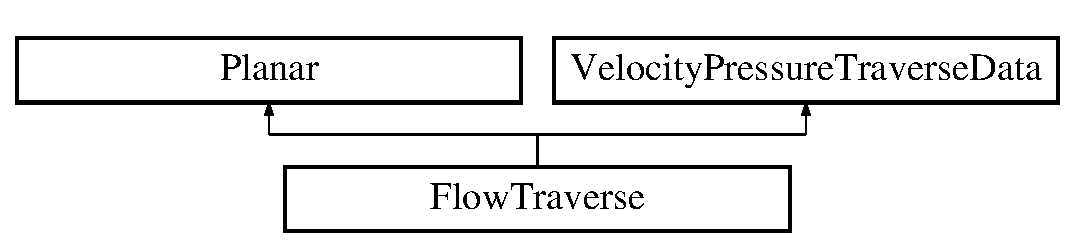
\includegraphics[height=2.000000cm]{dc/dd3/class_flow_traverse}
\end{center}
\end{figure}
\subsection*{Public Member Functions}
\begin{DoxyCompactItemize}
\item 
\mbox{\Hypertarget{class_flow_traverse_a95f14b9d4fb9722bad65752022813d06}\label{class_flow_traverse_a95f14b9d4fb9722bad65752022813d06}} 
{\bfseries Flow\+Traverse} (double circular\+Duct\+Diameter, double tdx, double pbx, double psx, double pitot\+Tube\+Coefficient, std\+::vector$<$ std\+::vector$<$ double $>$ $>$ traverse\+Hole\+Data)
\item 
\mbox{\Hypertarget{class_flow_traverse_ac96fdb9b848320a5fa9a8585ce6c0214}\label{class_flow_traverse_ac96fdb9b848320a5fa9a8585ce6c0214}} 
{\bfseries Flow\+Traverse} (double length, double width, double tdx, double pbx, double psx, double pitot\+Tube\+Coefficient, std\+::vector$<$ std\+::vector$<$ double $>$ $>$ traverse\+Hole\+Data, unsigned no\+Inlet\+Boxes=1)
\end{DoxyCompactItemize}
\subsection*{Additional Inherited Members}


\subsection{Detailed Description}


Definition at line 51 of file Planar.\+h.



The documentation for this class was generated from the following files\+:\begin{DoxyCompactItemize}
\item 
include/fans/Planar.\+h\item 
src/fans/Planar.\+cpp\end{DoxyCompactItemize}

\hypertarget{class_fluid_power}{}\section{Fluid\+Power Class Reference}
\label{class_fluid_power}\index{Fluid\+Power@{Fluid\+Power}}


Contains the skeleton of \hyperlink{class_fluid_power}{Fluid\+Power} class. \hyperlink{class_fluid_power_a2691f6efdbd5e71aa91e087c6b1c197b}{calculate()}\+: Calculates the fluid power.  




{\ttfamily \#include $<$Fluid\+Power.\+h$>$}

\subsection*{Public Member Functions}
\begin{DoxyCompactItemize}
\item 
\hyperlink{class_fluid_power_a9bf61af202e27b9e41ed284b4b1643ee}{Fluid\+Power} (double specific\+Gravity, double flow\+Rate, double head)
\item 
\hyperlink{class_fluid_power_a4c0369fcf0c85d28fa9afbdd56358fd4}{Fluid\+Power} (double flow\+Rate, const double inlet\+Pressure, const double outlet\+Pressure, const double compressibility\+Factor)
\item 
double \hyperlink{class_fluid_power_a2691f6efdbd5e71aa91e087c6b1c197b}{calculate} ()
\item 
\hyperlink{class_fluid_power_a9bf61af202e27b9e41ed284b4b1643ee}{Fluid\+Power} (double specific\+Gravity, double flow\+Rate, double head)
\item 
\hyperlink{class_fluid_power_a4c0369fcf0c85d28fa9afbdd56358fd4}{Fluid\+Power} (double flow\+Rate, const double inlet\+Pressure, const double outlet\+Pressure, const double compressibility\+Factor)
\item 
double \hyperlink{class_fluid_power_a2691f6efdbd5e71aa91e087c6b1c197b}{calculate} ()
\item 
\hyperlink{class_fluid_power_a9bf61af202e27b9e41ed284b4b1643ee}{Fluid\+Power} (double specific\+Gravity, double flow\+Rate, double head)
\item 
\hyperlink{class_fluid_power_a4c0369fcf0c85d28fa9afbdd56358fd4}{Fluid\+Power} (double flow\+Rate, const double inlet\+Pressure, const double outlet\+Pressure, const double compressibility\+Factor)
\item 
double \hyperlink{class_fluid_power_a2691f6efdbd5e71aa91e087c6b1c197b}{calculate} ()
\end{DoxyCompactItemize}


\subsection{Detailed Description}
Contains the skeleton of \hyperlink{class_fluid_power}{Fluid\+Power} class. \hyperlink{class_fluid_power_a2691f6efdbd5e71aa91e087c6b1c197b}{calculate()}\+: Calculates the fluid power. 

\begin{DoxyAuthor}{Author}
Subhankar Mishra (mishras) 

Gina Accawi (accawigk) 
\end{DoxyAuthor}


\begin{DoxyAuthor}{Author}
Subhankar Mishra (mishras) 

Gina Accawi (accawigk) 
\end{DoxyAuthor}


\begin{DoxyAuthor}{Author}
Subhankar Mishra (mishras) 

Gina Accawi (accawigk) 
\end{DoxyAuthor}


Definition at line 14 of file Fluid\+Power.\+h.



\subsection{Constructor \& Destructor Documentation}
\mbox{\Hypertarget{class_fluid_power_a9bf61af202e27b9e41ed284b4b1643ee}\label{class_fluid_power_a9bf61af202e27b9e41ed284b4b1643ee}} 
\index{Fluid\+Power@{Fluid\+Power}!Fluid\+Power@{Fluid\+Power}}
\index{Fluid\+Power@{Fluid\+Power}!Fluid\+Power@{Fluid\+Power}}
\subsubsection{\texorpdfstring{Fluid\+Power()}{FluidPower()}\hspace{0.1cm}{\footnotesize\ttfamily [1/6]}}
{\footnotesize\ttfamily Fluid\+Power\+::\+Fluid\+Power (\begin{DoxyParamCaption}\item[{double}]{specific\+Gravity,  }\item[{double}]{flow\+Rate,  }\item[{double}]{head }\end{DoxyParamCaption})\hspace{0.3cm}{\ttfamily [inline]}}

\hyperlink{class_fluid_power}{Fluid\+Power} constructor for pump systems 
\begin{DoxyParams}{Parameters}
{\em specific\+Gravity} & double, specified gravity -\/ unitless \\
\hline
{\em flow\+Rate} & double, rate of flow in gpm \\
\hline
{\em head} & double, pump head measured in feet \\
\hline
\end{DoxyParams}


Definition at line 22 of file Fluid\+Power.\+h.

\mbox{\Hypertarget{class_fluid_power_a4c0369fcf0c85d28fa9afbdd56358fd4}\label{class_fluid_power_a4c0369fcf0c85d28fa9afbdd56358fd4}} 
\index{Fluid\+Power@{Fluid\+Power}!Fluid\+Power@{Fluid\+Power}}
\index{Fluid\+Power@{Fluid\+Power}!Fluid\+Power@{Fluid\+Power}}
\subsubsection{\texorpdfstring{Fluid\+Power()}{FluidPower()}\hspace{0.1cm}{\footnotesize\ttfamily [2/6]}}
{\footnotesize\ttfamily Fluid\+Power\+::\+Fluid\+Power (\begin{DoxyParamCaption}\item[{double}]{flow\+Rate,  }\item[{const double}]{inlet\+Pressure,  }\item[{const double}]{outlet\+Pressure,  }\item[{const double}]{compressibility\+Factor }\end{DoxyParamCaption})\hspace{0.3cm}{\ttfamily [inline]}}

\hyperlink{class_fluid_power}{Fluid\+Power} constructor for Fan systems 
\begin{DoxyParams}{Parameters}
{\em flow\+Rate} & double, rate of flow in cfm \\
\hline
{\em inlet\+Pressure} & double, in inches of water column, gauge \\
\hline
{\em outlet\+Pressure} & double, in inches of water column, gauge \\
\hline
{\em compressibility\+Factor} & double, unitless \\
\hline
\end{DoxyParams}


Definition at line 33 of file Fluid\+Power.\+h.

\mbox{\Hypertarget{class_fluid_power_a9bf61af202e27b9e41ed284b4b1643ee}\label{class_fluid_power_a9bf61af202e27b9e41ed284b4b1643ee}} 
\index{Fluid\+Power@{Fluid\+Power}!Fluid\+Power@{Fluid\+Power}}
\index{Fluid\+Power@{Fluid\+Power}!Fluid\+Power@{Fluid\+Power}}
\subsubsection{\texorpdfstring{Fluid\+Power()}{FluidPower()}\hspace{0.1cm}{\footnotesize\ttfamily [3/6]}}
{\footnotesize\ttfamily Fluid\+Power\+::\+Fluid\+Power (\begin{DoxyParamCaption}\item[{double}]{specific\+Gravity,  }\item[{double}]{flow\+Rate,  }\item[{double}]{head }\end{DoxyParamCaption})\hspace{0.3cm}{\ttfamily [inline]}}

\hyperlink{class_fluid_power}{Fluid\+Power} constructor for pump systems 
\begin{DoxyParams}{Parameters}
{\em specific\+Gravity} & double, specified gravity -\/ unitless \\
\hline
{\em flow\+Rate} & double, rate of flow in gpm \\
\hline
{\em head} & double, pump head measured in feet \\
\hline
\end{DoxyParams}


Definition at line 22 of file Fluid\+Power.\+h.

\mbox{\Hypertarget{class_fluid_power_a4c0369fcf0c85d28fa9afbdd56358fd4}\label{class_fluid_power_a4c0369fcf0c85d28fa9afbdd56358fd4}} 
\index{Fluid\+Power@{Fluid\+Power}!Fluid\+Power@{Fluid\+Power}}
\index{Fluid\+Power@{Fluid\+Power}!Fluid\+Power@{Fluid\+Power}}
\subsubsection{\texorpdfstring{Fluid\+Power()}{FluidPower()}\hspace{0.1cm}{\footnotesize\ttfamily [4/6]}}
{\footnotesize\ttfamily Fluid\+Power\+::\+Fluid\+Power (\begin{DoxyParamCaption}\item[{double}]{flow\+Rate,  }\item[{const double}]{inlet\+Pressure,  }\item[{const double}]{outlet\+Pressure,  }\item[{const double}]{compressibility\+Factor }\end{DoxyParamCaption})\hspace{0.3cm}{\ttfamily [inline]}}

\hyperlink{class_fluid_power}{Fluid\+Power} constructor for Fan systems 
\begin{DoxyParams}{Parameters}
{\em flow\+Rate} & double, rate of flow in cfm \\
\hline
{\em inlet\+Pressure} & double, in inches of water column, gauge \\
\hline
{\em outlet\+Pressure} & double, in inches of water column, gauge \\
\hline
{\em compressibility\+Factor} & double, unitless \\
\hline
\end{DoxyParams}


Definition at line 33 of file Fluid\+Power.\+h.

\mbox{\Hypertarget{class_fluid_power_a9bf61af202e27b9e41ed284b4b1643ee}\label{class_fluid_power_a9bf61af202e27b9e41ed284b4b1643ee}} 
\index{Fluid\+Power@{Fluid\+Power}!Fluid\+Power@{Fluid\+Power}}
\index{Fluid\+Power@{Fluid\+Power}!Fluid\+Power@{Fluid\+Power}}
\subsubsection{\texorpdfstring{Fluid\+Power()}{FluidPower()}\hspace{0.1cm}{\footnotesize\ttfamily [5/6]}}
{\footnotesize\ttfamily Fluid\+Power\+::\+Fluid\+Power (\begin{DoxyParamCaption}\item[{double}]{specific\+Gravity,  }\item[{double}]{flow\+Rate,  }\item[{double}]{head }\end{DoxyParamCaption})\hspace{0.3cm}{\ttfamily [inline]}}

\hyperlink{class_fluid_power}{Fluid\+Power} constructor for pump systems 
\begin{DoxyParams}{Parameters}
{\em specific\+Gravity} & double, specified gravity -\/ unitless \\
\hline
{\em flow\+Rate} & double, rate of flow in gpm \\
\hline
{\em head} & double, pump head measured in feet \\
\hline
\end{DoxyParams}


Definition at line 22 of file Fluid\+Power.\+h.

\mbox{\Hypertarget{class_fluid_power_a4c0369fcf0c85d28fa9afbdd56358fd4}\label{class_fluid_power_a4c0369fcf0c85d28fa9afbdd56358fd4}} 
\index{Fluid\+Power@{Fluid\+Power}!Fluid\+Power@{Fluid\+Power}}
\index{Fluid\+Power@{Fluid\+Power}!Fluid\+Power@{Fluid\+Power}}
\subsubsection{\texorpdfstring{Fluid\+Power()}{FluidPower()}\hspace{0.1cm}{\footnotesize\ttfamily [6/6]}}
{\footnotesize\ttfamily Fluid\+Power\+::\+Fluid\+Power (\begin{DoxyParamCaption}\item[{double}]{flow\+Rate,  }\item[{const double}]{inlet\+Pressure,  }\item[{const double}]{outlet\+Pressure,  }\item[{const double}]{compressibility\+Factor }\end{DoxyParamCaption})\hspace{0.3cm}{\ttfamily [inline]}}

\hyperlink{class_fluid_power}{Fluid\+Power} constructor for Fan systems 
\begin{DoxyParams}{Parameters}
{\em flow\+Rate} & double, rate of flow in cfm \\
\hline
{\em inlet\+Pressure} & double, in inches of water column, gauge \\
\hline
{\em outlet\+Pressure} & double, in inches of water column, gauge \\
\hline
{\em compressibility\+Factor} & double, unitless \\
\hline
\end{DoxyParams}


Definition at line 33 of file Fluid\+Power.\+h.



\subsection{Member Function Documentation}
\mbox{\Hypertarget{class_fluid_power_a2691f6efdbd5e71aa91e087c6b1c197b}\label{class_fluid_power_a2691f6efdbd5e71aa91e087c6b1c197b}} 
\index{Fluid\+Power@{Fluid\+Power}!calculate@{calculate}}
\index{calculate@{calculate}!Fluid\+Power@{Fluid\+Power}}
\subsubsection{\texorpdfstring{calculate()}{calculate()}\hspace{0.1cm}{\footnotesize\ttfamily [1/3]}}
{\footnotesize\ttfamily double Fluid\+Power\+::calculate (\begin{DoxyParamCaption}{ }\end{DoxyParamCaption})\hspace{0.3cm}{\ttfamily [inline]}}

Calculates pump or fan fluid power in kw, depending on the number of constructor inputs (is\+Pump) \begin{DoxyReturn}{Returns}
double, fluid power 
\end{DoxyReturn}


Definition at line 42 of file Fluid\+Power.\+h.

\mbox{\Hypertarget{class_fluid_power_a2691f6efdbd5e71aa91e087c6b1c197b}\label{class_fluid_power_a2691f6efdbd5e71aa91e087c6b1c197b}} 
\index{Fluid\+Power@{Fluid\+Power}!calculate@{calculate}}
\index{calculate@{calculate}!Fluid\+Power@{Fluid\+Power}}
\subsubsection{\texorpdfstring{calculate()}{calculate()}\hspace{0.1cm}{\footnotesize\ttfamily [2/3]}}
{\footnotesize\ttfamily double Fluid\+Power\+::calculate (\begin{DoxyParamCaption}{ }\end{DoxyParamCaption})\hspace{0.3cm}{\ttfamily [inline]}}

Calculates pump or fan fluid power in kw, depending on the number of constructor inputs (is\+Pump) \begin{DoxyReturn}{Returns}
double, fluid power 
\end{DoxyReturn}


Definition at line 42 of file Fluid\+Power.\+h.

\mbox{\Hypertarget{class_fluid_power_a2691f6efdbd5e71aa91e087c6b1c197b}\label{class_fluid_power_a2691f6efdbd5e71aa91e087c6b1c197b}} 
\index{Fluid\+Power@{Fluid\+Power}!calculate@{calculate}}
\index{calculate@{calculate}!Fluid\+Power@{Fluid\+Power}}
\subsubsection{\texorpdfstring{calculate()}{calculate()}\hspace{0.1cm}{\footnotesize\ttfamily [3/3]}}
{\footnotesize\ttfamily double Fluid\+Power\+::calculate (\begin{DoxyParamCaption}{ }\end{DoxyParamCaption})\hspace{0.3cm}{\ttfamily [inline]}}

Calculates pump or fan fluid power in kw, depending on the number of constructor inputs (is\+Pump) \begin{DoxyReturn}{Returns}
double, fluid power 
\end{DoxyReturn}


Definition at line 42 of file Fluid\+Power.\+h.



The documentation for this class was generated from the following file\+:\begin{DoxyCompactItemize}
\item 
\+\_\+\+C\+Pack\+\_\+\+Packages/\+Darwin/\+S\+T\+G\+Z/amo\+\_\+tools\+\_\+suite-\/-\/\+Darwin-\/x86\+\_\+64/amo\+\_\+tools\+\_\+suite/include/calculator/pump/Fluid\+Power.\+h\end{DoxyCompactItemize}

\hypertarget{class_fuel_fired_energy_equivalency}{}\section{Fuel\+Fired\+Energy\+Equivalency Class Reference}
\label{class_fuel_fired_energy_equivalency}\index{Fuel\+Fired\+Energy\+Equivalency@{Fuel\+Fired\+Energy\+Equivalency}}


{\ttfamily \#include $<$Energy\+Equivalency.\+h$>$}

\subsection*{Public Member Functions}
\begin{DoxyCompactItemize}
\item 
\hyperlink{class_fuel_fired_energy_equivalency_ac4ba992ccb3d4a19eb29f14898031690}{Fuel\+Fired\+Energy\+Equivalency} (double electrically\+Heated\+Efficiency, double fuel\+Fired\+Efficiency, double electrical\+Heat\+Input)
\item 
double \hyperlink{class_fuel_fired_energy_equivalency_ad4bd750677313895d8345c7eaf8308bd}{get\+Electrically\+Heated\+Efficiency} () const
\item 
void \hyperlink{class_fuel_fired_energy_equivalency_a2e8e166d9824ee07805cd790eff5e361}{set\+Electrically\+Heated\+Efficiency} (double electrically\+Heated\+Efficiency)
\item 
double \hyperlink{class_fuel_fired_energy_equivalency_ac8695c1fe3dcffeab60b5305239d2a58}{get\+Fuel\+Fired\+Efficiency} () const
\item 
void \hyperlink{class_fuel_fired_energy_equivalency_a510b4a7c1231faeeebca02fa0b1723ae}{set\+Fuel\+Fired\+Efficiency} (double fuel\+Fired\+Efficiency)
\item 
double \hyperlink{class_fuel_fired_energy_equivalency_a7d5878809c01a9243aa999406cddd4a9}{get\+Electrical\+Heat\+Input} () const
\item 
void \hyperlink{class_fuel_fired_energy_equivalency_a222836bfef1cb0caec0adafc2ef6b7ea}{set\+Electrical\+Heat\+Input} (double electrical\+Heat\+Input)
\item 
double \hyperlink{class_fuel_fired_energy_equivalency_a6bf68595ca361dd4135d0c84c2fbe6d9}{get\+Fuel\+Fired\+Heat\+Input} ()
\end{DoxyCompactItemize}


\subsection{Detailed Description}
Fuel Fired Energy Equivalency calculator class Used to calculate the fuel-\/fired heat input that is equivalent to the electric heat input. 

Definition at line 125 of file Energy\+Equivalency.\+h.



\subsection{Constructor \& Destructor Documentation}
\mbox{\Hypertarget{class_fuel_fired_energy_equivalency_ac4ba992ccb3d4a19eb29f14898031690}\label{class_fuel_fired_energy_equivalency_ac4ba992ccb3d4a19eb29f14898031690}} 
\index{Fuel\+Fired\+Energy\+Equivalency@{Fuel\+Fired\+Energy\+Equivalency}!Fuel\+Fired\+Energy\+Equivalency@{Fuel\+Fired\+Energy\+Equivalency}}
\index{Fuel\+Fired\+Energy\+Equivalency@{Fuel\+Fired\+Energy\+Equivalency}!Fuel\+Fired\+Energy\+Equivalency@{Fuel\+Fired\+Energy\+Equivalency}}
\subsubsection{\texorpdfstring{Fuel\+Fired\+Energy\+Equivalency()}{FuelFiredEnergyEquivalency()}}
{\footnotesize\ttfamily Fuel\+Fired\+Energy\+Equivalency\+::\+Fuel\+Fired\+Energy\+Equivalency (\begin{DoxyParamCaption}\item[{double}]{electrically\+Heated\+Efficiency,  }\item[{double}]{fuel\+Fired\+Efficiency,  }\item[{double}]{electrical\+Heat\+Input }\end{DoxyParamCaption})\hspace{0.3cm}{\ttfamily [inline]}}

Constructor for the fuel-\/fired equivalency calculator


\begin{DoxyParams}{Parameters}
{\em electrically\+Heated\+Efficiency} & double, electrically heated equipment efficiency as \% \\
\hline
{\em fuel\+Fired\+Efficiency} & double, fuel-\/fired equipment efficiency as \% \\
\hline
{\em electrical\+Heat\+Input} & double, heat input for electrically heated equipment in kW \\
\hline
\end{DoxyParams}


Definition at line 137 of file Energy\+Equivalency.\+h.



\subsection{Member Function Documentation}
\mbox{\Hypertarget{class_fuel_fired_energy_equivalency_a7d5878809c01a9243aa999406cddd4a9}\label{class_fuel_fired_energy_equivalency_a7d5878809c01a9243aa999406cddd4a9}} 
\index{Fuel\+Fired\+Energy\+Equivalency@{Fuel\+Fired\+Energy\+Equivalency}!get\+Electrical\+Heat\+Input@{get\+Electrical\+Heat\+Input}}
\index{get\+Electrical\+Heat\+Input@{get\+Electrical\+Heat\+Input}!Fuel\+Fired\+Energy\+Equivalency@{Fuel\+Fired\+Energy\+Equivalency}}
\subsubsection{\texorpdfstring{get\+Electrical\+Heat\+Input()}{getElectricalHeatInput()}}
{\footnotesize\ttfamily double Fuel\+Fired\+Energy\+Equivalency\+::get\+Electrical\+Heat\+Input (\begin{DoxyParamCaption}{ }\end{DoxyParamCaption}) const\hspace{0.3cm}{\ttfamily [inline]}}

Getter for the heat input for electrically heated equipment

\begin{DoxyReturn}{Returns}
double, heat input for electrically heated equipment in kW 
\end{DoxyReturn}


Definition at line 196 of file Energy\+Equivalency.\+h.

\mbox{\Hypertarget{class_fuel_fired_energy_equivalency_ad4bd750677313895d8345c7eaf8308bd}\label{class_fuel_fired_energy_equivalency_ad4bd750677313895d8345c7eaf8308bd}} 
\index{Fuel\+Fired\+Energy\+Equivalency@{Fuel\+Fired\+Energy\+Equivalency}!get\+Electrically\+Heated\+Efficiency@{get\+Electrically\+Heated\+Efficiency}}
\index{get\+Electrically\+Heated\+Efficiency@{get\+Electrically\+Heated\+Efficiency}!Fuel\+Fired\+Energy\+Equivalency@{Fuel\+Fired\+Energy\+Equivalency}}
\subsubsection{\texorpdfstring{get\+Electrically\+Heated\+Efficiency()}{getElectricallyHeatedEfficiency()}}
{\footnotesize\ttfamily double Fuel\+Fired\+Energy\+Equivalency\+::get\+Electrically\+Heated\+Efficiency (\begin{DoxyParamCaption}{ }\end{DoxyParamCaption}) const\hspace{0.3cm}{\ttfamily [inline]}}

Getter for the electrically heated equipment efficiency

\begin{DoxyReturn}{Returns}
double, electrically heated equipment efficiency as \% 
\end{DoxyReturn}


Definition at line 158 of file Energy\+Equivalency.\+h.

\mbox{\Hypertarget{class_fuel_fired_energy_equivalency_ac8695c1fe3dcffeab60b5305239d2a58}\label{class_fuel_fired_energy_equivalency_ac8695c1fe3dcffeab60b5305239d2a58}} 
\index{Fuel\+Fired\+Energy\+Equivalency@{Fuel\+Fired\+Energy\+Equivalency}!get\+Fuel\+Fired\+Efficiency@{get\+Fuel\+Fired\+Efficiency}}
\index{get\+Fuel\+Fired\+Efficiency@{get\+Fuel\+Fired\+Efficiency}!Fuel\+Fired\+Energy\+Equivalency@{Fuel\+Fired\+Energy\+Equivalency}}
\subsubsection{\texorpdfstring{get\+Fuel\+Fired\+Efficiency()}{getFuelFiredEfficiency()}}
{\footnotesize\ttfamily double Fuel\+Fired\+Energy\+Equivalency\+::get\+Fuel\+Fired\+Efficiency (\begin{DoxyParamCaption}{ }\end{DoxyParamCaption}) const\hspace{0.3cm}{\ttfamily [inline]}}

Getter for the fuel-\/fired equipment efficiency

\begin{DoxyReturn}{Returns}
double, fuel-\/fired equipment efficiency as \% 
\end{DoxyReturn}


Definition at line 177 of file Energy\+Equivalency.\+h.

\mbox{\Hypertarget{class_fuel_fired_energy_equivalency_a6bf68595ca361dd4135d0c84c2fbe6d9}\label{class_fuel_fired_energy_equivalency_a6bf68595ca361dd4135d0c84c2fbe6d9}} 
\index{Fuel\+Fired\+Energy\+Equivalency@{Fuel\+Fired\+Energy\+Equivalency}!get\+Fuel\+Fired\+Heat\+Input@{get\+Fuel\+Fired\+Heat\+Input}}
\index{get\+Fuel\+Fired\+Heat\+Input@{get\+Fuel\+Fired\+Heat\+Input}!Fuel\+Fired\+Energy\+Equivalency@{Fuel\+Fired\+Energy\+Equivalency}}
\subsubsection{\texorpdfstring{get\+Fuel\+Fired\+Heat\+Input()}{getFuelFiredHeatInput()}}
{\footnotesize\ttfamily double Fuel\+Fired\+Energy\+Equivalency\+::get\+Fuel\+Fired\+Heat\+Input (\begin{DoxyParamCaption}{ }\end{DoxyParamCaption})}

Gets the equivalent fuel-\/fired heat input \begin{DoxyReturn}{Returns}
double, equivalent fuel-\/fired heat input in MM Btu/hr 
\end{DoxyReturn}


Definition at line 16 of file Energy\+Equivalency.\+cpp.

\mbox{\Hypertarget{class_fuel_fired_energy_equivalency_a222836bfef1cb0caec0adafc2ef6b7ea}\label{class_fuel_fired_energy_equivalency_a222836bfef1cb0caec0adafc2ef6b7ea}} 
\index{Fuel\+Fired\+Energy\+Equivalency@{Fuel\+Fired\+Energy\+Equivalency}!set\+Electrical\+Heat\+Input@{set\+Electrical\+Heat\+Input}}
\index{set\+Electrical\+Heat\+Input@{set\+Electrical\+Heat\+Input}!Fuel\+Fired\+Energy\+Equivalency@{Fuel\+Fired\+Energy\+Equivalency}}
\subsubsection{\texorpdfstring{set\+Electrical\+Heat\+Input()}{setElectricalHeatInput()}}
{\footnotesize\ttfamily void Fuel\+Fired\+Energy\+Equivalency\+::set\+Electrical\+Heat\+Input (\begin{DoxyParamCaption}\item[{double}]{electrical\+Heat\+Input }\end{DoxyParamCaption})\hspace{0.3cm}{\ttfamily [inline]}}

Sets the heat input for electrically heated equipment


\begin{DoxyParams}{Parameters}
{\em electrical\+Heat\+Input} & double, heat input for electrically heated equipment in kW \\
\hline
\end{DoxyParams}


Definition at line 206 of file Energy\+Equivalency.\+h.

\mbox{\Hypertarget{class_fuel_fired_energy_equivalency_a2e8e166d9824ee07805cd790eff5e361}\label{class_fuel_fired_energy_equivalency_a2e8e166d9824ee07805cd790eff5e361}} 
\index{Fuel\+Fired\+Energy\+Equivalency@{Fuel\+Fired\+Energy\+Equivalency}!set\+Electrically\+Heated\+Efficiency@{set\+Electrically\+Heated\+Efficiency}}
\index{set\+Electrically\+Heated\+Efficiency@{set\+Electrically\+Heated\+Efficiency}!Fuel\+Fired\+Energy\+Equivalency@{Fuel\+Fired\+Energy\+Equivalency}}
\subsubsection{\texorpdfstring{set\+Electrically\+Heated\+Efficiency()}{setElectricallyHeatedEfficiency()}}
{\footnotesize\ttfamily void Fuel\+Fired\+Energy\+Equivalency\+::set\+Electrically\+Heated\+Efficiency (\begin{DoxyParamCaption}\item[{double}]{electrically\+Heated\+Efficiency }\end{DoxyParamCaption})\hspace{0.3cm}{\ttfamily [inline]}}

Sets the electrically heated equipment efficiency


\begin{DoxyParams}{Parameters}
{\em electrically\+Heated\+Efficiency} & double, electrically heated equipment efficiency as \% \\
\hline
\end{DoxyParams}


Definition at line 168 of file Energy\+Equivalency.\+h.

\mbox{\Hypertarget{class_fuel_fired_energy_equivalency_a510b4a7c1231faeeebca02fa0b1723ae}\label{class_fuel_fired_energy_equivalency_a510b4a7c1231faeeebca02fa0b1723ae}} 
\index{Fuel\+Fired\+Energy\+Equivalency@{Fuel\+Fired\+Energy\+Equivalency}!set\+Fuel\+Fired\+Efficiency@{set\+Fuel\+Fired\+Efficiency}}
\index{set\+Fuel\+Fired\+Efficiency@{set\+Fuel\+Fired\+Efficiency}!Fuel\+Fired\+Energy\+Equivalency@{Fuel\+Fired\+Energy\+Equivalency}}
\subsubsection{\texorpdfstring{set\+Fuel\+Fired\+Efficiency()}{setFuelFiredEfficiency()}}
{\footnotesize\ttfamily void Fuel\+Fired\+Energy\+Equivalency\+::set\+Fuel\+Fired\+Efficiency (\begin{DoxyParamCaption}\item[{double}]{fuel\+Fired\+Efficiency }\end{DoxyParamCaption})\hspace{0.3cm}{\ttfamily [inline]}}

Sets the fuel-\/fired equipment efficiency


\begin{DoxyParams}{Parameters}
{\em fuel\+Fired\+Efficiency} & double, fuel-\/fired equipment efficiency as \% \\
\hline
\end{DoxyParams}


Definition at line 187 of file Energy\+Equivalency.\+h.



The documentation for this class was generated from the following files\+:\begin{DoxyCompactItemize}
\item 
include/calculator/furnace/\hyperlink{_energy_equivalency_8h}{Energy\+Equivalency.\+h}\item 
src/calculator/furnace/\hyperlink{_energy_equivalency_8cpp}{Energy\+Equivalency.\+cpp}\end{DoxyCompactItemize}

\hypertarget{class_gas_compositions}{}\section{Gas\+Compositions Class Reference}
\label{class_gas_compositions}\index{Gas\+Compositions@{Gas\+Compositions}}


{\ttfamily \#include $<$Gas\+Flue\+Gas\+Material.\+h$>$}

\subsection*{Public Member Functions}
\begin{DoxyCompactItemize}
\item 
\hyperlink{class_gas_compositions_ad0021d4285883374f8904f9465e41920}{Gas\+Compositions} (std\+::string substance, const double C\+H4, const double C2\+H6, const double N2, const double H2, const double C3\+H8, const double C4\+H10\+\_\+\+Cn\+H2n, const double H2O, const double CO, const double C\+O2, const double S\+O2, const double O2)
\item 
double \hyperlink{class_gas_compositions_a2028a42c136e057a6153b7bfa68d63e6}{get\+Gas\+By\+Vol} (const std\+::string \&gas\+Name) const
\item 
\mbox{\Hypertarget{class_gas_compositions_a7ebcdf1c991bd70f28eb845e45d62afd}\label{class_gas_compositions_a7ebcdf1c991bd70f28eb845e45d62afd}} 
double {\bfseries get\+Heating\+Value} () const
\item 
\mbox{\Hypertarget{class_gas_compositions_a4f891acb4f8dc3992703155c6ba7ccb0}\label{class_gas_compositions_a4f891acb4f8dc3992703155c6ba7ccb0}} 
double {\bfseries get\+Specific\+Gravity} () const
\item 
\mbox{\Hypertarget{class_gas_compositions_a4f6408254477960648440da460099e2d}\label{class_gas_compositions_a4f6408254477960648440da460099e2d}} 
double {\bfseries calculate\+Excess\+Air} (double flue\+Gas\+O2)
\item 
std\+::string \hyperlink{class_gas_compositions_abad9554bca9b68cd970eae11bdd3c505}{get\+Substance} () const
\item 
int \hyperlink{class_gas_compositions_a9668decdb2b5065c8ee3c59c207b9d51}{get\+ID} () const
\item 
void \hyperlink{class_gas_compositions_a9fc3ebfcbda7134b67ed76a39b4c94cc}{set\+ID} (const int id)
\item 
\hyperlink{class_gas_compositions_ad0021d4285883374f8904f9465e41920}{Gas\+Compositions} (std\+::string substance, const double C\+H4, const double C2\+H6, const double N2, const double H2, const double C3\+H8, const double C4\+H10\+\_\+\+Cn\+H2n, const double H2O, const double CO, const double C\+O2, const double S\+O2, const double O2)
\item 
double \hyperlink{class_gas_compositions_a2028a42c136e057a6153b7bfa68d63e6}{get\+Gas\+By\+Vol} (const std\+::string \&gas\+Name) const
\item 
\mbox{\Hypertarget{class_gas_compositions_a7ebcdf1c991bd70f28eb845e45d62afd}\label{class_gas_compositions_a7ebcdf1c991bd70f28eb845e45d62afd}} 
double {\bfseries get\+Heating\+Value} () const
\item 
\mbox{\Hypertarget{class_gas_compositions_a4f891acb4f8dc3992703155c6ba7ccb0}\label{class_gas_compositions_a4f891acb4f8dc3992703155c6ba7ccb0}} 
double {\bfseries get\+Specific\+Gravity} () const
\item 
\mbox{\Hypertarget{class_gas_compositions_a4f6408254477960648440da460099e2d}\label{class_gas_compositions_a4f6408254477960648440da460099e2d}} 
double {\bfseries calculate\+Excess\+Air} (double flue\+Gas\+O2)
\item 
std\+::string \hyperlink{class_gas_compositions_abad9554bca9b68cd970eae11bdd3c505}{get\+Substance} () const
\item 
int \hyperlink{class_gas_compositions_a9668decdb2b5065c8ee3c59c207b9d51}{get\+ID} () const
\item 
void \hyperlink{class_gas_compositions_a9fc3ebfcbda7134b67ed76a39b4c94cc}{set\+ID} (const int id)
\item 
\hyperlink{class_gas_compositions_ad0021d4285883374f8904f9465e41920}{Gas\+Compositions} (std\+::string substance, const double C\+H4, const double C2\+H6, const double N2, const double H2, const double C3\+H8, const double C4\+H10\+\_\+\+Cn\+H2n, const double H2O, const double CO, const double C\+O2, const double S\+O2, const double O2)
\item 
double \hyperlink{class_gas_compositions_a2028a42c136e057a6153b7bfa68d63e6}{get\+Gas\+By\+Vol} (const std\+::string \&gas\+Name) const
\item 
\mbox{\Hypertarget{class_gas_compositions_a7ebcdf1c991bd70f28eb845e45d62afd}\label{class_gas_compositions_a7ebcdf1c991bd70f28eb845e45d62afd}} 
double {\bfseries get\+Heating\+Value} () const
\item 
\mbox{\Hypertarget{class_gas_compositions_a4f891acb4f8dc3992703155c6ba7ccb0}\label{class_gas_compositions_a4f891acb4f8dc3992703155c6ba7ccb0}} 
double {\bfseries get\+Specific\+Gravity} () const
\item 
\mbox{\Hypertarget{class_gas_compositions_a4f6408254477960648440da460099e2d}\label{class_gas_compositions_a4f6408254477960648440da460099e2d}} 
double {\bfseries calculate\+Excess\+Air} (double flue\+Gas\+O2)
\item 
std\+::string \hyperlink{class_gas_compositions_abad9554bca9b68cd970eae11bdd3c505}{get\+Substance} () const
\item 
int \hyperlink{class_gas_compositions_a9668decdb2b5065c8ee3c59c207b9d51}{get\+ID} () const
\item 
void \hyperlink{class_gas_compositions_a9fc3ebfcbda7134b67ed76a39b4c94cc}{set\+ID} (const int id)
\end{DoxyCompactItemize}
\subsection*{Friends}
\begin{DoxyCompactItemize}
\item 
\mbox{\Hypertarget{class_gas_compositions_a399a12526ca1c801e9b82aef418254f6}\label{class_gas_compositions_a399a12526ca1c801e9b82aef418254f6}} 
class {\bfseries Gas\+Flue\+Gas\+Material}
\item 
\mbox{\Hypertarget{class_gas_compositions_a0102f3b3c0cbf96db6c49f071fa5e7cc}\label{class_gas_compositions_a0102f3b3c0cbf96db6c49f071fa5e7cc}} 
class {\bfseries S\+Q\+Lite}
\end{DoxyCompactItemize}


\subsection{Detailed Description}
Gas Compositions class Contains the gas compositions of a gas mixture. 

Definition at line 73 of file Gas\+Flue\+Gas\+Material.\+h.



\subsection{Constructor \& Destructor Documentation}
\mbox{\Hypertarget{class_gas_compositions_ad0021d4285883374f8904f9465e41920}\label{class_gas_compositions_ad0021d4285883374f8904f9465e41920}} 
\index{Gas\+Compositions@{Gas\+Compositions}!Gas\+Compositions@{Gas\+Compositions}}
\index{Gas\+Compositions@{Gas\+Compositions}!Gas\+Compositions@{Gas\+Compositions}}
\subsubsection{\texorpdfstring{Gas\+Compositions()}{GasCompositions()}\hspace{0.1cm}{\footnotesize\ttfamily [1/3]}}
{\footnotesize\ttfamily Gas\+Compositions\+::\+Gas\+Compositions (\begin{DoxyParamCaption}\item[{std\+::string}]{substance,  }\item[{const double}]{C\+H4,  }\item[{const double}]{C2\+H6,  }\item[{const double}]{N2,  }\item[{const double}]{H2,  }\item[{const double}]{C3\+H8,  }\item[{const double}]{C4\+H10\+\_\+\+Cn\+H2n,  }\item[{const double}]{H2O,  }\item[{const double}]{CO,  }\item[{const double}]{C\+O2,  }\item[{const double}]{S\+O2,  }\item[{const double}]{O2 }\end{DoxyParamCaption})\hspace{0.3cm}{\ttfamily [inline]}}

Constructor for \hyperlink{class_gas_compositions}{Gas\+Compositions} with which flue gas losses will be calculated. All molecule parameters are the percentage of that molecule present in the fuel


\begin{DoxyParams}{Parameters}
{\em substance} & name -\/ string \\
\hline
{\em C\+H4} & \% -\/ double \\
\hline
{\em C2\+H6} & \% -\/ double \\
\hline
{\em N2} & \% -\/ double \\
\hline
{\em H2} & \% -\/ double \\
\hline
{\em C3\+H8} & \% -\/ double \\
\hline
{\em C4\+H10\+\_\+\+Cn\+H2n} & \% -\/ double \\
\hline
{\em H2O} & \% -\/ double \\
\hline
{\em CO} & \% -\/ double \\
\hline
{\em C\+O2} & \% -\/ double \\
\hline
{\em S\+O2} & \% -\/ double \\
\hline
{\em O2} & \% -\/ double \\
\hline
\end{DoxyParams}


Definition at line 93 of file Gas\+Flue\+Gas\+Material.\+h.

\mbox{\Hypertarget{class_gas_compositions_ad0021d4285883374f8904f9465e41920}\label{class_gas_compositions_ad0021d4285883374f8904f9465e41920}} 
\index{Gas\+Compositions@{Gas\+Compositions}!Gas\+Compositions@{Gas\+Compositions}}
\index{Gas\+Compositions@{Gas\+Compositions}!Gas\+Compositions@{Gas\+Compositions}}
\subsubsection{\texorpdfstring{Gas\+Compositions()}{GasCompositions()}\hspace{0.1cm}{\footnotesize\ttfamily [2/3]}}
{\footnotesize\ttfamily Gas\+Compositions\+::\+Gas\+Compositions (\begin{DoxyParamCaption}\item[{std\+::string}]{substance,  }\item[{const double}]{C\+H4,  }\item[{const double}]{C2\+H6,  }\item[{const double}]{N2,  }\item[{const double}]{H2,  }\item[{const double}]{C3\+H8,  }\item[{const double}]{C4\+H10\+\_\+\+Cn\+H2n,  }\item[{const double}]{H2O,  }\item[{const double}]{CO,  }\item[{const double}]{C\+O2,  }\item[{const double}]{S\+O2,  }\item[{const double}]{O2 }\end{DoxyParamCaption})\hspace{0.3cm}{\ttfamily [inline]}}

Constructor for \hyperlink{class_gas_compositions}{Gas\+Compositions} with which flue gas losses will be calculated. All molecule parameters are the percentage of that molecule present in the fuel


\begin{DoxyParams}{Parameters}
{\em substance} & name -\/ string \\
\hline
{\em C\+H4} & \% -\/ double \\
\hline
{\em C2\+H6} & \% -\/ double \\
\hline
{\em N2} & \% -\/ double \\
\hline
{\em H2} & \% -\/ double \\
\hline
{\em C3\+H8} & \% -\/ double \\
\hline
{\em C4\+H10\+\_\+\+Cn\+H2n} & \% -\/ double \\
\hline
{\em H2O} & \% -\/ double \\
\hline
{\em CO} & \% -\/ double \\
\hline
{\em C\+O2} & \% -\/ double \\
\hline
{\em S\+O2} & \% -\/ double \\
\hline
{\em O2} & \% -\/ double \\
\hline
\end{DoxyParams}


Definition at line 93 of file Gas\+Flue\+Gas\+Material.\+h.

\mbox{\Hypertarget{class_gas_compositions_ad0021d4285883374f8904f9465e41920}\label{class_gas_compositions_ad0021d4285883374f8904f9465e41920}} 
\index{Gas\+Compositions@{Gas\+Compositions}!Gas\+Compositions@{Gas\+Compositions}}
\index{Gas\+Compositions@{Gas\+Compositions}!Gas\+Compositions@{Gas\+Compositions}}
\subsubsection{\texorpdfstring{Gas\+Compositions()}{GasCompositions()}\hspace{0.1cm}{\footnotesize\ttfamily [3/3]}}
{\footnotesize\ttfamily Gas\+Compositions\+::\+Gas\+Compositions (\begin{DoxyParamCaption}\item[{std\+::string}]{substance,  }\item[{const double}]{C\+H4,  }\item[{const double}]{C2\+H6,  }\item[{const double}]{N2,  }\item[{const double}]{H2,  }\item[{const double}]{C3\+H8,  }\item[{const double}]{C4\+H10\+\_\+\+Cn\+H2n,  }\item[{const double}]{H2O,  }\item[{const double}]{CO,  }\item[{const double}]{C\+O2,  }\item[{const double}]{S\+O2,  }\item[{const double}]{O2 }\end{DoxyParamCaption})\hspace{0.3cm}{\ttfamily [inline]}}

Constructor for \hyperlink{class_gas_compositions}{Gas\+Compositions} with which flue gas losses will be calculated. All molecule parameters are the percentage of that molecule present in the fuel


\begin{DoxyParams}{Parameters}
{\em substance} & name -\/ string \\
\hline
{\em C\+H4} & \% -\/ double \\
\hline
{\em C2\+H6} & \% -\/ double \\
\hline
{\em N2} & \% -\/ double \\
\hline
{\em H2} & \% -\/ double \\
\hline
{\em C3\+H8} & \% -\/ double \\
\hline
{\em C4\+H10\+\_\+\+Cn\+H2n} & \% -\/ double \\
\hline
{\em H2O} & \% -\/ double \\
\hline
{\em CO} & \% -\/ double \\
\hline
{\em C\+O2} & \% -\/ double \\
\hline
{\em S\+O2} & \% -\/ double \\
\hline
{\em O2} & \% -\/ double \\
\hline
\end{DoxyParams}


Definition at line 93 of file Gas\+Flue\+Gas\+Material.\+h.



\subsection{Member Function Documentation}
\mbox{\Hypertarget{class_gas_compositions_a2028a42c136e057a6153b7bfa68d63e6}\label{class_gas_compositions_a2028a42c136e057a6153b7bfa68d63e6}} 
\index{Gas\+Compositions@{Gas\+Compositions}!get\+Gas\+By\+Vol@{get\+Gas\+By\+Vol}}
\index{get\+Gas\+By\+Vol@{get\+Gas\+By\+Vol}!Gas\+Compositions@{Gas\+Compositions}}
\subsubsection{\texorpdfstring{get\+Gas\+By\+Vol()}{getGasByVol()}\hspace{0.1cm}{\footnotesize\ttfamily [1/3]}}
{\footnotesize\ttfamily double Gas\+Compositions\+::get\+Gas\+By\+Vol (\begin{DoxyParamCaption}\item[{const std\+::string \&}]{gas\+Name }\end{DoxyParamCaption}) const\hspace{0.3cm}{\ttfamily [inline]}}

Gets the gas by its name


\begin{DoxyParams}{Parameters}
{\em gas\+Name} & const string, name of gas\\
\hline
\end{DoxyParams}
\begin{DoxyReturn}{Returns}
double, composition by volume as \% 
\end{DoxyReturn}


Definition at line 137 of file Gas\+Flue\+Gas\+Material.\+h.

\mbox{\Hypertarget{class_gas_compositions_a2028a42c136e057a6153b7bfa68d63e6}\label{class_gas_compositions_a2028a42c136e057a6153b7bfa68d63e6}} 
\index{Gas\+Compositions@{Gas\+Compositions}!get\+Gas\+By\+Vol@{get\+Gas\+By\+Vol}}
\index{get\+Gas\+By\+Vol@{get\+Gas\+By\+Vol}!Gas\+Compositions@{Gas\+Compositions}}
\subsubsection{\texorpdfstring{get\+Gas\+By\+Vol()}{getGasByVol()}\hspace{0.1cm}{\footnotesize\ttfamily [2/3]}}
{\footnotesize\ttfamily double Gas\+Compositions\+::get\+Gas\+By\+Vol (\begin{DoxyParamCaption}\item[{const std\+::string \&}]{gas\+Name }\end{DoxyParamCaption}) const\hspace{0.3cm}{\ttfamily [inline]}}

Gets the gas by its name


\begin{DoxyParams}{Parameters}
{\em gas\+Name} & const string, name of gas\\
\hline
\end{DoxyParams}
\begin{DoxyReturn}{Returns}
double, composition by volume as \% 
\end{DoxyReturn}


Definition at line 137 of file Gas\+Flue\+Gas\+Material.\+h.

\mbox{\Hypertarget{class_gas_compositions_a2028a42c136e057a6153b7bfa68d63e6}\label{class_gas_compositions_a2028a42c136e057a6153b7bfa68d63e6}} 
\index{Gas\+Compositions@{Gas\+Compositions}!get\+Gas\+By\+Vol@{get\+Gas\+By\+Vol}}
\index{get\+Gas\+By\+Vol@{get\+Gas\+By\+Vol}!Gas\+Compositions@{Gas\+Compositions}}
\subsubsection{\texorpdfstring{get\+Gas\+By\+Vol()}{getGasByVol()}\hspace{0.1cm}{\footnotesize\ttfamily [3/3]}}
{\footnotesize\ttfamily double Gas\+Compositions\+::get\+Gas\+By\+Vol (\begin{DoxyParamCaption}\item[{const std\+::string \&}]{gas\+Name }\end{DoxyParamCaption}) const\hspace{0.3cm}{\ttfamily [inline]}}

Gets the gas by its name


\begin{DoxyParams}{Parameters}
{\em gas\+Name} & const string, name of gas\\
\hline
\end{DoxyParams}
\begin{DoxyReturn}{Returns}
double, composition by volume as \% 
\end{DoxyReturn}


Definition at line 137 of file Gas\+Flue\+Gas\+Material.\+h.

\mbox{\Hypertarget{class_gas_compositions_a9668decdb2b5065c8ee3c59c207b9d51}\label{class_gas_compositions_a9668decdb2b5065c8ee3c59c207b9d51}} 
\index{Gas\+Compositions@{Gas\+Compositions}!get\+ID@{get\+ID}}
\index{get\+ID@{get\+ID}!Gas\+Compositions@{Gas\+Compositions}}
\subsubsection{\texorpdfstring{get\+I\+D()}{getID()}\hspace{0.1cm}{\footnotesize\ttfamily [1/3]}}
{\footnotesize\ttfamily int Gas\+Compositions\+::get\+ID (\begin{DoxyParamCaption}{ }\end{DoxyParamCaption}) const\hspace{0.3cm}{\ttfamily [inline]}}

Gets the ID of gas

\begin{DoxyReturn}{Returns}
int, ID of gas 
\end{DoxyReturn}


Definition at line 162 of file Gas\+Flue\+Gas\+Material.\+h.

\mbox{\Hypertarget{class_gas_compositions_a9668decdb2b5065c8ee3c59c207b9d51}\label{class_gas_compositions_a9668decdb2b5065c8ee3c59c207b9d51}} 
\index{Gas\+Compositions@{Gas\+Compositions}!get\+ID@{get\+ID}}
\index{get\+ID@{get\+ID}!Gas\+Compositions@{Gas\+Compositions}}
\subsubsection{\texorpdfstring{get\+I\+D()}{getID()}\hspace{0.1cm}{\footnotesize\ttfamily [2/3]}}
{\footnotesize\ttfamily int Gas\+Compositions\+::get\+ID (\begin{DoxyParamCaption}{ }\end{DoxyParamCaption}) const\hspace{0.3cm}{\ttfamily [inline]}}

Gets the ID of gas

\begin{DoxyReturn}{Returns}
int, ID of gas 
\end{DoxyReturn}


Definition at line 162 of file Gas\+Flue\+Gas\+Material.\+h.

\mbox{\Hypertarget{class_gas_compositions_a9668decdb2b5065c8ee3c59c207b9d51}\label{class_gas_compositions_a9668decdb2b5065c8ee3c59c207b9d51}} 
\index{Gas\+Compositions@{Gas\+Compositions}!get\+ID@{get\+ID}}
\index{get\+ID@{get\+ID}!Gas\+Compositions@{Gas\+Compositions}}
\subsubsection{\texorpdfstring{get\+I\+D()}{getID()}\hspace{0.1cm}{\footnotesize\ttfamily [3/3]}}
{\footnotesize\ttfamily int Gas\+Compositions\+::get\+ID (\begin{DoxyParamCaption}{ }\end{DoxyParamCaption}) const\hspace{0.3cm}{\ttfamily [inline]}}

Gets the ID of gas

\begin{DoxyReturn}{Returns}
int, ID of gas 
\end{DoxyReturn}


Definition at line 162 of file Gas\+Flue\+Gas\+Material.\+h.

\mbox{\Hypertarget{class_gas_compositions_abad9554bca9b68cd970eae11bdd3c505}\label{class_gas_compositions_abad9554bca9b68cd970eae11bdd3c505}} 
\index{Gas\+Compositions@{Gas\+Compositions}!get\+Substance@{get\+Substance}}
\index{get\+Substance@{get\+Substance}!Gas\+Compositions@{Gas\+Compositions}}
\subsubsection{\texorpdfstring{get\+Substance()}{getSubstance()}\hspace{0.1cm}{\footnotesize\ttfamily [1/3]}}
{\footnotesize\ttfamily std\+::string Gas\+Compositions\+::get\+Substance (\begin{DoxyParamCaption}{ }\end{DoxyParamCaption}) const}

Gets the name of substance

\begin{DoxyReturn}{Returns}
string, name of substance 
\end{DoxyReturn}


Definition at line 13 of file Gas\+Flue\+Gas\+Material.\+cpp.

\mbox{\Hypertarget{class_gas_compositions_abad9554bca9b68cd970eae11bdd3c505}\label{class_gas_compositions_abad9554bca9b68cd970eae11bdd3c505}} 
\index{Gas\+Compositions@{Gas\+Compositions}!get\+Substance@{get\+Substance}}
\index{get\+Substance@{get\+Substance}!Gas\+Compositions@{Gas\+Compositions}}
\subsubsection{\texorpdfstring{get\+Substance()}{getSubstance()}\hspace{0.1cm}{\footnotesize\ttfamily [2/3]}}
{\footnotesize\ttfamily std\+::string Gas\+Compositions\+::get\+Substance (\begin{DoxyParamCaption}{ }\end{DoxyParamCaption}) const}

Gets the name of substance

\begin{DoxyReturn}{Returns}
string, name of substance 
\end{DoxyReturn}
\mbox{\Hypertarget{class_gas_compositions_abad9554bca9b68cd970eae11bdd3c505}\label{class_gas_compositions_abad9554bca9b68cd970eae11bdd3c505}} 
\index{Gas\+Compositions@{Gas\+Compositions}!get\+Substance@{get\+Substance}}
\index{get\+Substance@{get\+Substance}!Gas\+Compositions@{Gas\+Compositions}}
\subsubsection{\texorpdfstring{get\+Substance()}{getSubstance()}\hspace{0.1cm}{\footnotesize\ttfamily [3/3]}}
{\footnotesize\ttfamily std\+::string Gas\+Compositions\+::get\+Substance (\begin{DoxyParamCaption}{ }\end{DoxyParamCaption}) const}

Gets the name of substance

\begin{DoxyReturn}{Returns}
string, name of substance 
\end{DoxyReturn}
\mbox{\Hypertarget{class_gas_compositions_a9fc3ebfcbda7134b67ed76a39b4c94cc}\label{class_gas_compositions_a9fc3ebfcbda7134b67ed76a39b4c94cc}} 
\index{Gas\+Compositions@{Gas\+Compositions}!set\+ID@{set\+ID}}
\index{set\+ID@{set\+ID}!Gas\+Compositions@{Gas\+Compositions}}
\subsubsection{\texorpdfstring{set\+I\+D()}{setID()}\hspace{0.1cm}{\footnotesize\ttfamily [1/3]}}
{\footnotesize\ttfamily void Gas\+Compositions\+::set\+ID (\begin{DoxyParamCaption}\item[{const int}]{id }\end{DoxyParamCaption})\hspace{0.3cm}{\ttfamily [inline]}}

Sets the ID of gas


\begin{DoxyParams}{Parameters}
{\em id} & const int, ID number for gas\\
\hline
\end{DoxyParams}
\begin{DoxyReturn}{Returns}
nothing 
\end{DoxyReturn}


Definition at line 173 of file Gas\+Flue\+Gas\+Material.\+h.

\mbox{\Hypertarget{class_gas_compositions_a9fc3ebfcbda7134b67ed76a39b4c94cc}\label{class_gas_compositions_a9fc3ebfcbda7134b67ed76a39b4c94cc}} 
\index{Gas\+Compositions@{Gas\+Compositions}!set\+ID@{set\+ID}}
\index{set\+ID@{set\+ID}!Gas\+Compositions@{Gas\+Compositions}}
\subsubsection{\texorpdfstring{set\+I\+D()}{setID()}\hspace{0.1cm}{\footnotesize\ttfamily [2/3]}}
{\footnotesize\ttfamily void Gas\+Compositions\+::set\+ID (\begin{DoxyParamCaption}\item[{const int}]{id }\end{DoxyParamCaption})\hspace{0.3cm}{\ttfamily [inline]}}

Sets the ID of gas


\begin{DoxyParams}{Parameters}
{\em id} & const int, ID number for gas\\
\hline
\end{DoxyParams}
\begin{DoxyReturn}{Returns}
nothing 
\end{DoxyReturn}


Definition at line 173 of file Gas\+Flue\+Gas\+Material.\+h.

\mbox{\Hypertarget{class_gas_compositions_a9fc3ebfcbda7134b67ed76a39b4c94cc}\label{class_gas_compositions_a9fc3ebfcbda7134b67ed76a39b4c94cc}} 
\index{Gas\+Compositions@{Gas\+Compositions}!set\+ID@{set\+ID}}
\index{set\+ID@{set\+ID}!Gas\+Compositions@{Gas\+Compositions}}
\subsubsection{\texorpdfstring{set\+I\+D()}{setID()}\hspace{0.1cm}{\footnotesize\ttfamily [3/3]}}
{\footnotesize\ttfamily void Gas\+Compositions\+::set\+ID (\begin{DoxyParamCaption}\item[{const int}]{id }\end{DoxyParamCaption})\hspace{0.3cm}{\ttfamily [inline]}}

Sets the ID of gas


\begin{DoxyParams}{Parameters}
{\em id} & const int, ID number for gas\\
\hline
\end{DoxyParams}
\begin{DoxyReturn}{Returns}
nothing 
\end{DoxyReturn}


Definition at line 173 of file Gas\+Flue\+Gas\+Material.\+h.



The documentation for this class was generated from the following files\+:\begin{DoxyCompactItemize}
\item 
\+\_\+\+C\+Pack\+\_\+\+Packages/\+Darwin/\+S\+T\+G\+Z/amo\+\_\+tools\+\_\+suite-\/-\/\+Darwin-\/x86\+\_\+64/amo\+\_\+tools\+\_\+suite/include/calculator/losses/\hyperlink{___c_pack___packages_2_darwin_2_s_t_g_z_2amo__tools__suite--_darwin-x86__64_2amo__tools__suite_2004d7ef7737e3755a6d819de5baaee93}{Gas\+Flue\+Gas\+Material.\+h}\item 
src/calculator/losses/\hyperlink{_gas_flue_gas_material_8cpp}{Gas\+Flue\+Gas\+Material.\+cpp}\end{DoxyCompactItemize}

\hypertarget{class_gas_cooling_losses}{}\section{Gas\+Cooling\+Losses Class Reference}
\label{class_gas_cooling_losses}\index{Gas\+Cooling\+Losses@{Gas\+Cooling\+Losses}}


{\ttfamily \#include $<$Gas\+Cooling\+Losses.\+h$>$}

\subsection*{Public Member Functions}
\begin{DoxyCompactItemize}
\item 
\hyperlink{class_gas_cooling_losses_a0afd445c71ebcc1b8de23adeb15741b6}{Gas\+Cooling\+Losses} (const double flow\+Rate, const double initial\+Temperature, const double final\+Temperature, const double specific\+Heat, const double correction\+Factor, const double gas\+Density)
\item 
double \hyperlink{class_gas_cooling_losses_a3c18b6d1ef3124d883daf85560ec7bd7}{get\+Heat\+Loss} () const
\item 
\hyperlink{class_gas_cooling_losses_a0afd445c71ebcc1b8de23adeb15741b6}{Gas\+Cooling\+Losses} (const double flow\+Rate, const double initial\+Temperature, const double final\+Temperature, const double specific\+Heat, const double correction\+Factor, const double gas\+Density)
\item 
double \hyperlink{class_gas_cooling_losses_a3c18b6d1ef3124d883daf85560ec7bd7}{get\+Heat\+Loss} () const
\item 
\hyperlink{class_gas_cooling_losses_a0afd445c71ebcc1b8de23adeb15741b6}{Gas\+Cooling\+Losses} (const double flow\+Rate, const double initial\+Temperature, const double final\+Temperature, const double specific\+Heat, const double correction\+Factor, const double gas\+Density)
\item 
double \hyperlink{class_gas_cooling_losses_a3c18b6d1ef3124d883daf85560ec7bd7}{get\+Heat\+Loss} () const
\end{DoxyCompactItemize}


\subsection{Detailed Description}
Gas Cooling Losses class Contains all of the properties of a cooling system and its gas media. Used to calculate how much heat loss is caused by the cooling components and their cooling media (a gas). 

Definition at line 21 of file Gas\+Cooling\+Losses.\+h.



\subsection{Constructor \& Destructor Documentation}
\mbox{\Hypertarget{class_gas_cooling_losses_a0afd445c71ebcc1b8de23adeb15741b6}\label{class_gas_cooling_losses_a0afd445c71ebcc1b8de23adeb15741b6}} 
\index{Gas\+Cooling\+Losses@{Gas\+Cooling\+Losses}!Gas\+Cooling\+Losses@{Gas\+Cooling\+Losses}}
\index{Gas\+Cooling\+Losses@{Gas\+Cooling\+Losses}!Gas\+Cooling\+Losses@{Gas\+Cooling\+Losses}}
\subsubsection{\texorpdfstring{Gas\+Cooling\+Losses()}{GasCoolingLosses()}\hspace{0.1cm}{\footnotesize\ttfamily [1/3]}}
{\footnotesize\ttfamily Gas\+Cooling\+Losses\+::\+Gas\+Cooling\+Losses (\begin{DoxyParamCaption}\item[{const double}]{flow\+Rate,  }\item[{const double}]{initial\+Temperature,  }\item[{const double}]{final\+Temperature,  }\item[{const double}]{specific\+Heat,  }\item[{const double}]{correction\+Factor,  }\item[{const double}]{gas\+Density }\end{DoxyParamCaption})\hspace{0.3cm}{\ttfamily [inline]}}

Constructor for the gas cooling losses (including air) with all inputs specified


\begin{DoxyParams}{Parameters}
{\em flow\+Rate} & double, Air or gas volumetric flow rate in S\+C\+FM (ft³/min) \\
\hline
{\em initial\+Temperature} & double, \hyperlink{class_inlet}{Inlet} temperature of air or gas in °F \\
\hline
{\em final\+Temperature} & double, Outlet temperature of air or gas in °F \\
\hline
{\em specific\+Heat} & double, Specific heat of gas or air at average air temperature in Btu/(scf$\ast$°F) \\
\hline
{\em correction\+Factor} & double, Correction factor -\/ unitless \\
\hline
\end{DoxyParams}


Definition at line 35 of file Gas\+Cooling\+Losses.\+h.

\mbox{\Hypertarget{class_gas_cooling_losses_a0afd445c71ebcc1b8de23adeb15741b6}\label{class_gas_cooling_losses_a0afd445c71ebcc1b8de23adeb15741b6}} 
\index{Gas\+Cooling\+Losses@{Gas\+Cooling\+Losses}!Gas\+Cooling\+Losses@{Gas\+Cooling\+Losses}}
\index{Gas\+Cooling\+Losses@{Gas\+Cooling\+Losses}!Gas\+Cooling\+Losses@{Gas\+Cooling\+Losses}}
\subsubsection{\texorpdfstring{Gas\+Cooling\+Losses()}{GasCoolingLosses()}\hspace{0.1cm}{\footnotesize\ttfamily [2/3]}}
{\footnotesize\ttfamily Gas\+Cooling\+Losses\+::\+Gas\+Cooling\+Losses (\begin{DoxyParamCaption}\item[{const double}]{flow\+Rate,  }\item[{const double}]{initial\+Temperature,  }\item[{const double}]{final\+Temperature,  }\item[{const double}]{specific\+Heat,  }\item[{const double}]{correction\+Factor,  }\item[{const double}]{gas\+Density }\end{DoxyParamCaption})\hspace{0.3cm}{\ttfamily [inline]}}

Constructor for the gas cooling losses (including air) with all inputs specified


\begin{DoxyParams}{Parameters}
{\em flow\+Rate} & double, Air or gas volumetric flow rate in S\+C\+FM (ft³/min) \\
\hline
{\em initial\+Temperature} & double, \hyperlink{class_inlet}{Inlet} temperature of air or gas in °F \\
\hline
{\em final\+Temperature} & double, Outlet temperature of air or gas in °F \\
\hline
{\em specific\+Heat} & double, Specific heat of gas or air at average air temperature in Btu/(scf$\ast$°F) \\
\hline
{\em correction\+Factor} & double, Correction factor -\/ unitless \\
\hline
\end{DoxyParams}


Definition at line 35 of file Gas\+Cooling\+Losses.\+h.

\mbox{\Hypertarget{class_gas_cooling_losses_a0afd445c71ebcc1b8de23adeb15741b6}\label{class_gas_cooling_losses_a0afd445c71ebcc1b8de23adeb15741b6}} 
\index{Gas\+Cooling\+Losses@{Gas\+Cooling\+Losses}!Gas\+Cooling\+Losses@{Gas\+Cooling\+Losses}}
\index{Gas\+Cooling\+Losses@{Gas\+Cooling\+Losses}!Gas\+Cooling\+Losses@{Gas\+Cooling\+Losses}}
\subsubsection{\texorpdfstring{Gas\+Cooling\+Losses()}{GasCoolingLosses()}\hspace{0.1cm}{\footnotesize\ttfamily [3/3]}}
{\footnotesize\ttfamily Gas\+Cooling\+Losses\+::\+Gas\+Cooling\+Losses (\begin{DoxyParamCaption}\item[{const double}]{flow\+Rate,  }\item[{const double}]{initial\+Temperature,  }\item[{const double}]{final\+Temperature,  }\item[{const double}]{specific\+Heat,  }\item[{const double}]{correction\+Factor,  }\item[{const double}]{gas\+Density }\end{DoxyParamCaption})\hspace{0.3cm}{\ttfamily [inline]}}

Constructor for the gas cooling losses (including air) with all inputs specified


\begin{DoxyParams}{Parameters}
{\em flow\+Rate} & double, Air or gas volumetric flow rate in S\+C\+FM (ft³/min) \\
\hline
{\em initial\+Temperature} & double, \hyperlink{class_inlet}{Inlet} temperature of air or gas in °F \\
\hline
{\em final\+Temperature} & double, Outlet temperature of air or gas in °F \\
\hline
{\em specific\+Heat} & double, Specific heat of gas or air at average air temperature in Btu/(scf$\ast$°F) \\
\hline
{\em correction\+Factor} & double, Correction factor -\/ unitless \\
\hline
\end{DoxyParams}


Definition at line 35 of file Gas\+Cooling\+Losses.\+h.



\subsection{Member Function Documentation}
\mbox{\Hypertarget{class_gas_cooling_losses_a3c18b6d1ef3124d883daf85560ec7bd7}\label{class_gas_cooling_losses_a3c18b6d1ef3124d883daf85560ec7bd7}} 
\index{Gas\+Cooling\+Losses@{Gas\+Cooling\+Losses}!get\+Heat\+Loss@{get\+Heat\+Loss}}
\index{get\+Heat\+Loss@{get\+Heat\+Loss}!Gas\+Cooling\+Losses@{Gas\+Cooling\+Losses}}
\subsubsection{\texorpdfstring{get\+Heat\+Loss()}{getHeatLoss()}\hspace{0.1cm}{\footnotesize\ttfamily [1/3]}}
{\footnotesize\ttfamily double Gas\+Cooling\+Losses\+::get\+Heat\+Loss (\begin{DoxyParamCaption}{ }\end{DoxyParamCaption}) const}

Gets the total heat loss \begin{DoxyReturn}{Returns}
double, heat loss in btu/hr 
\end{DoxyReturn}


Definition at line 11 of file Gas\+Cooling\+Losses.\+cpp.

\mbox{\Hypertarget{class_gas_cooling_losses_a3c18b6d1ef3124d883daf85560ec7bd7}\label{class_gas_cooling_losses_a3c18b6d1ef3124d883daf85560ec7bd7}} 
\index{Gas\+Cooling\+Losses@{Gas\+Cooling\+Losses}!get\+Heat\+Loss@{get\+Heat\+Loss}}
\index{get\+Heat\+Loss@{get\+Heat\+Loss}!Gas\+Cooling\+Losses@{Gas\+Cooling\+Losses}}
\subsubsection{\texorpdfstring{get\+Heat\+Loss()}{getHeatLoss()}\hspace{0.1cm}{\footnotesize\ttfamily [2/3]}}
{\footnotesize\ttfamily double Gas\+Cooling\+Losses\+::get\+Heat\+Loss (\begin{DoxyParamCaption}{ }\end{DoxyParamCaption}) const}

Gets the total heat loss \begin{DoxyReturn}{Returns}
double, heat loss in btu/hr 
\end{DoxyReturn}
\mbox{\Hypertarget{class_gas_cooling_losses_a3c18b6d1ef3124d883daf85560ec7bd7}\label{class_gas_cooling_losses_a3c18b6d1ef3124d883daf85560ec7bd7}} 
\index{Gas\+Cooling\+Losses@{Gas\+Cooling\+Losses}!get\+Heat\+Loss@{get\+Heat\+Loss}}
\index{get\+Heat\+Loss@{get\+Heat\+Loss}!Gas\+Cooling\+Losses@{Gas\+Cooling\+Losses}}
\subsubsection{\texorpdfstring{get\+Heat\+Loss()}{getHeatLoss()}\hspace{0.1cm}{\footnotesize\ttfamily [3/3]}}
{\footnotesize\ttfamily double Gas\+Cooling\+Losses\+::get\+Heat\+Loss (\begin{DoxyParamCaption}{ }\end{DoxyParamCaption}) const}

Gets the total heat loss \begin{DoxyReturn}{Returns}
double, heat loss in btu/hr 
\end{DoxyReturn}


The documentation for this class was generated from the following files\+:\begin{DoxyCompactItemize}
\item 
\+\_\+\+C\+Pack\+\_\+\+Packages/\+Darwin/\+S\+T\+G\+Z/amo\+\_\+tools\+\_\+suite-\/-\/\+Darwin-\/x86\+\_\+64/amo\+\_\+tools\+\_\+suite/include/calculator/losses/\hyperlink{___c_pack___packages_2_darwin_2_s_t_g_z_2amo__tools__suite--_darwin-x86__64_2amo__tools__suite_2a205f1c3faea20d1b572055736aa9a09}{Gas\+Cooling\+Losses.\+h}\item 
src/calculator/losses/\hyperlink{_gas_cooling_losses_8cpp}{Gas\+Cooling\+Losses.\+cpp}\end{DoxyCompactItemize}

\hypertarget{class_gas_flue_gas_material}{}\section{Gas\+Flue\+Gas\+Material Class Reference}
\label{class_gas_flue_gas_material}\index{Gas\+Flue\+Gas\+Material@{Gas\+Flue\+Gas\+Material}}


{\ttfamily \#include $<$Gas\+Flue\+Gas\+Material.\+h$>$}

\subsection*{Public Member Functions}
\begin{DoxyCompactItemize}
\item 
\hyperlink{class_gas_flue_gas_material_aca4ce48fe0feea4e6032679652f38c98}{Gas\+Flue\+Gas\+Material} (const double flue\+Gas\+Temperature, const double excess\+Air\+Percentage, const double combustion\+Air\+Temperature, \hyperlink{class_gas_compositions}{Gas\+Compositions} compositions, const double fuel\+Temperature)
\item 
double \hyperlink{class_gas_flue_gas_material_ad9990d400536c6e8c7c53b9212de400b}{get\+Heat\+Loss} ()
\end{DoxyCompactItemize}


\subsection{Detailed Description}
Gas Flue Gas Material class Contains all of the properties of a gas flue gas material. Used to calculate the heat loss caused by carrying the products of combustion out of the system through the flue. 

Definition at line 242 of file Gas\+Flue\+Gas\+Material.\+h.



\subsection{Constructor \& Destructor Documentation}
\mbox{\Hypertarget{class_gas_flue_gas_material_aca4ce48fe0feea4e6032679652f38c98}\label{class_gas_flue_gas_material_aca4ce48fe0feea4e6032679652f38c98}} 
\index{Gas\+Flue\+Gas\+Material@{Gas\+Flue\+Gas\+Material}!Gas\+Flue\+Gas\+Material@{Gas\+Flue\+Gas\+Material}}
\index{Gas\+Flue\+Gas\+Material@{Gas\+Flue\+Gas\+Material}!Gas\+Flue\+Gas\+Material@{Gas\+Flue\+Gas\+Material}}
\subsubsection{\texorpdfstring{Gas\+Flue\+Gas\+Material()}{GasFlueGasMaterial()}}
{\footnotesize\ttfamily Gas\+Flue\+Gas\+Material\+::\+Gas\+Flue\+Gas\+Material (\begin{DoxyParamCaption}\item[{const double}]{flue\+Gas\+Temperature,  }\item[{const double}]{excess\+Air\+Percentage,  }\item[{const double}]{combustion\+Air\+Temperature,  }\item[{\hyperlink{class_gas_compositions}{Gas\+Compositions}}]{compositions,  }\item[{const double}]{fuel\+Temperature }\end{DoxyParamCaption})\hspace{0.3cm}{\ttfamily [inline]}}

Constructor for the flue gas losses with all inputs specified


\begin{DoxyParams}{Parameters}
{\em flue\+Gas\+Temperature} & double, \hyperlink{class_furnace}{Furnace} Flue Gas Temperature in °F \\
\hline
{\em excess\+Air\+Percentage} & double, Percent Excess Air, expressed in normal percentage (i.\+e. 9\% as 9 instead of 0.\+09) \\
\hline
{\em combustion\+Air\+Temperature} & double, Combustion Air Temperature in °F \\
\hline
{\em compositions} & -\/ Gas\+Composition, User defined gas compositions \\
\hline
{\em fuel\+Temperature} & double -\/ temperature of fuel \\
\hline
\end{DoxyParams}


Definition at line 253 of file Gas\+Flue\+Gas\+Material.\+h.



\subsection{Member Function Documentation}
\mbox{\Hypertarget{class_gas_flue_gas_material_ad9990d400536c6e8c7c53b9212de400b}\label{class_gas_flue_gas_material_ad9990d400536c6e8c7c53b9212de400b}} 
\index{Gas\+Flue\+Gas\+Material@{Gas\+Flue\+Gas\+Material}!get\+Heat\+Loss@{get\+Heat\+Loss}}
\index{get\+Heat\+Loss@{get\+Heat\+Loss}!Gas\+Flue\+Gas\+Material@{Gas\+Flue\+Gas\+Material}}
\subsubsection{\texorpdfstring{get\+Heat\+Loss()}{getHeatLoss()}}
{\footnotesize\ttfamily double Gas\+Flue\+Gas\+Material\+::get\+Heat\+Loss (\begin{DoxyParamCaption}{ }\end{DoxyParamCaption})}

Gets the heat loss

\begin{DoxyReturn}{Returns}
double, heat loss in btu/hr 
\end{DoxyReturn}


Definition at line 163 of file Gas\+Flue\+Gas\+Material.\+cpp.



The documentation for this class was generated from the following files\+:\begin{DoxyCompactItemize}
\item 
include/calculator/losses/\hyperlink{_gas_flue_gas_material_8h}{Gas\+Flue\+Gas\+Material.\+h}\item 
src/calculator/losses/\hyperlink{_gas_flue_gas_material_8cpp}{Gas\+Flue\+Gas\+Material.\+cpp}\end{DoxyCompactItemize}

\hypertarget{class_gas_load_charge_material}{}\section{Gas\+Load\+Charge\+Material Class Reference}
\label{class_gas_load_charge_material}\index{Gas\+Load\+Charge\+Material@{Gas\+Load\+Charge\+Material}}


{\ttfamily \#include $<$Gas\+Load\+Charge\+Material.\+h$>$}

\subsection*{Public Member Functions}
\begin{DoxyCompactItemize}
\item 
\hyperlink{class_gas_load_charge_material_a4ad94a94d25bad9eaeca4947d879f35f}{Gas\+Load\+Charge\+Material} (const \hyperlink{namespace_load_charge_material_a51d4263e865a5d86236622dd3fe23fd1}{Load\+Charge\+Material\+::\+Thermic\+Reaction\+Type} thermic\+Reaction\+Type, const double specific\+Heat\+Gas, const double feed\+Rate, const double percent\+Vapor, const double initial\+Temperature, const double discharge\+Temperature, const double specific\+Heat\+Vapor, const double percent\+Reacted, const double reaction\+Heat, const double additional\+Heat)
\item 
\hyperlink{namespace_load_charge_material_a51d4263e865a5d86236622dd3fe23fd1}{Load\+Charge\+Material\+::\+Thermic\+Reaction\+Type} \hyperlink{class_gas_load_charge_material_ac801f30ccf58ce98fdb6b8cdb0a9767f}{get\+Thermic\+Reaction\+Type} () const
\item 
void \hyperlink{class_gas_load_charge_material_ac48eb07a3008f1dc0ff433353b59536d}{set\+Thermic\+Reaction\+Type} (\hyperlink{namespace_load_charge_material_a51d4263e865a5d86236622dd3fe23fd1}{Load\+Charge\+Material\+::\+Thermic\+Reaction\+Type} thermic\+Reaction\+Type)
\item 
double \hyperlink{class_gas_load_charge_material_a66e956e7a52b1032a3e8a725f26fa580}{get\+Specific\+Heat\+Gas} () const
\item 
void \hyperlink{class_gas_load_charge_material_a07bf6d4ee9161683fbeb3baad16ea7be}{set\+Specific\+Heat\+Gas} (double specific\+Heat\+Gas)
\item 
double \hyperlink{class_gas_load_charge_material_ae14ebe9b7091a491166174968505b6ee}{get\+Feed\+Rate} () const
\item 
void \hyperlink{class_gas_load_charge_material_a922b728dfd109d1c1684d7dfad82ec8e}{set\+Feed\+Rate} (double feed\+Rate)
\item 
double \hyperlink{class_gas_load_charge_material_af8a83c3720d108baa196394105822db7}{get\+Initial\+Temperature} () const
\item 
void \hyperlink{class_gas_load_charge_material_aec9ddfce5e31099b6a047e3d98d80d47}{set\+Initial\+Temperature} (double initial\+Temperature)
\item 
double \hyperlink{class_gas_load_charge_material_a6baaf6ad65e2a3d1fa90b7c007bc3c53}{get\+Discharge\+Temperature} () const
\item 
void \hyperlink{class_gas_load_charge_material_a6c53344d5370a1e9b7321a530a6843c0}{set\+Discharge\+Temperature} (double discharge\+Temperature)
\item 
double \hyperlink{class_gas_load_charge_material_a9a07e86938bb831e51ac3f53f696a3c3}{get\+Specific\+Heat\+Vapor} () const
\item 
void \hyperlink{class_gas_load_charge_material_a7498eba84bb8bdfc5344f0e44418260b}{set\+Specific\+Heat\+Vapor} (double specific\+Heat\+Vapor)
\item 
double \hyperlink{class_gas_load_charge_material_af47b4c6c3e547325cadd81cbb09937ee}{get\+Percent\+Reacted} () const
\item 
void \hyperlink{class_gas_load_charge_material_a7142cb6bbfba53d640dd6f1590fe32f6}{set\+Percent\+Reacted} (double percent\+Reacted)
\item 
double \hyperlink{class_gas_load_charge_material_a605eaf21d1f25f27b53627aeb903c93d}{get\+Reaction\+Heat} () const
\item 
void \hyperlink{class_gas_load_charge_material_a721f02cbd0bfbb6ebe67c0da09f0b0f2}{set\+Reaction\+Heat} (double reaction\+Heat)
\item 
double \hyperlink{class_gas_load_charge_material_a5c01f171b61c01c93db6453cb122e1ba}{get\+Additional\+Heat} () const
\item 
void \hyperlink{class_gas_load_charge_material_a08ef5196ea9919dfc71be6744c7da08e}{set\+Additional\+Heat} (double additional\+Heat)
\item 
double \hyperlink{class_gas_load_charge_material_a19b8ecfad235b5824b0a88903cff667a}{get\+Percent\+Vapor} () const
\item 
void \hyperlink{class_gas_load_charge_material_acace81e16ef531acb0a68462ab0ed25d}{set\+Percent\+Vapor} (double percent\+Vapor)
\item 
std\+::string \hyperlink{class_gas_load_charge_material_a5f967841f196f6b0b35f32f9610092e3}{get\+Substance} () const
\item 
void \hyperlink{class_gas_load_charge_material_a20cc3df601d8daae9b8f8e7b0c53c2e3}{set\+Substance} (std\+::string substance)
\item 
std\+::size\+\_\+t \hyperlink{class_gas_load_charge_material_a32dc0d73857ebe4322cf525064713cf6}{get\+ID} () const
\item 
void \hyperlink{class_gas_load_charge_material_a24b43ba7c871453258f458a8c1f15232}{set\+ID} (const std\+::size\+\_\+t id)
\item 
double \hyperlink{class_gas_load_charge_material_a4f831537652ca09c4539982c626cc164}{get\+Total\+Heat} ()
\item 
\mbox{\Hypertarget{class_gas_load_charge_material_ac1d95bdf7d61d8ed98629aa17bf2c4b1}\label{class_gas_load_charge_material_ac1d95bdf7d61d8ed98629aa17bf2c4b1}} 
bool \hyperlink{class_gas_load_charge_material_ac1d95bdf7d61d8ed98629aa17bf2c4b1}{operator==} (const \hyperlink{class_gas_load_charge_material}{Gas\+Load\+Charge\+Material} \&rhs) const
\begin{DoxyCompactList}\small\item\em bool operator \end{DoxyCompactList}\item 
\mbox{\Hypertarget{class_gas_load_charge_material_ac6bc3f665a91fde01ebf6d1528cb7332}\label{class_gas_load_charge_material_ac6bc3f665a91fde01ebf6d1528cb7332}} 
bool \hyperlink{class_gas_load_charge_material_ac6bc3f665a91fde01ebf6d1528cb7332}{operator!=} (const \hyperlink{class_gas_load_charge_material}{Gas\+Load\+Charge\+Material} \&rhs) const
\begin{DoxyCompactList}\small\item\em bool operator \end{DoxyCompactList}\end{DoxyCompactItemize}
\subsection*{Friends}
\begin{DoxyCompactItemize}
\item 
\mbox{\Hypertarget{class_gas_load_charge_material_ac7d22f3ca36435f73d55df60dc799e14}\label{class_gas_load_charge_material_ac7d22f3ca36435f73d55df60dc799e14}} 
class {\bfseries S\+Q\+Lite}
\end{DoxyCompactItemize}


\subsection{Detailed Description}
Gas Load Charge Material class Contains all properties of a gas load charge material Used to find the heat required for a gas load charge material to be heated from the inlet temperature to the outlet temperature 

Definition at line 24 of file Gas\+Load\+Charge\+Material.\+h.



\subsection{Constructor \& Destructor Documentation}
\mbox{\Hypertarget{class_gas_load_charge_material_a4ad94a94d25bad9eaeca4947d879f35f}\label{class_gas_load_charge_material_a4ad94a94d25bad9eaeca4947d879f35f}} 
\index{Gas\+Load\+Charge\+Material@{Gas\+Load\+Charge\+Material}!Gas\+Load\+Charge\+Material@{Gas\+Load\+Charge\+Material}}
\index{Gas\+Load\+Charge\+Material@{Gas\+Load\+Charge\+Material}!Gas\+Load\+Charge\+Material@{Gas\+Load\+Charge\+Material}}
\subsubsection{\texorpdfstring{Gas\+Load\+Charge\+Material()}{GasLoadChargeMaterial()}}
{\footnotesize\ttfamily Gas\+Load\+Charge\+Material\+::\+Gas\+Load\+Charge\+Material (\begin{DoxyParamCaption}\item[{const \hyperlink{namespace_load_charge_material_a51d4263e865a5d86236622dd3fe23fd1}{Load\+Charge\+Material\+::\+Thermic\+Reaction\+Type}}]{thermic\+Reaction\+Type,  }\item[{const double}]{specific\+Heat\+Gas,  }\item[{const double}]{feed\+Rate,  }\item[{const double}]{percent\+Vapor,  }\item[{const double}]{initial\+Temperature,  }\item[{const double}]{discharge\+Temperature,  }\item[{const double}]{specific\+Heat\+Vapor,  }\item[{const double}]{percent\+Reacted,  }\item[{const double}]{reaction\+Heat,  }\item[{const double}]{additional\+Heat }\end{DoxyParamCaption})\hspace{0.3cm}{\ttfamily [inline]}}

Constructor for the gas load/charge material with all inputs specified 
\begin{DoxyParams}{Parameters}
{\em thermic\+Reaction\+Type} & Enumerated value for either endothermic or exothermic reactions \\
\hline
{\em specific\+Heat\+Gas} & Specific Heat of Gas in Btu/(lb$\ast$°F) \\
\hline
{\em feed\+Rate} & Feed Rate for Gas Mixture in lb/hr \\
\hline
{\em percent\+Vapor} & Vapor in Gas Mixture (\% of Total) \\
\hline
{\em initial\+Temperature} & Initial Temperature in °F \\
\hline
{\em discharge\+Temperature} & Discharge Temperature in °F \\
\hline
{\em specific\+Heat\+Vapor} & Specific Heat of Vapor in Btu/(lb$\ast$°F) \\
\hline
{\em percent\+Reacted} & Feed Gas Reacted (\% of Total) \\
\hline
{\em reaction\+Heat} & Heat of Reaction in Btu/lb \\
\hline
{\em additional\+Heat} & Additional Heat Required in Btu/hr \\
\hline
\end{DoxyParams}


Definition at line 40 of file Gas\+Load\+Charge\+Material.\+h.



\subsection{Member Function Documentation}
\mbox{\Hypertarget{class_gas_load_charge_material_a5c01f171b61c01c93db6453cb122e1ba}\label{class_gas_load_charge_material_a5c01f171b61c01c93db6453cb122e1ba}} 
\index{Gas\+Load\+Charge\+Material@{Gas\+Load\+Charge\+Material}!get\+Additional\+Heat@{get\+Additional\+Heat}}
\index{get\+Additional\+Heat@{get\+Additional\+Heat}!Gas\+Load\+Charge\+Material@{Gas\+Load\+Charge\+Material}}
\subsubsection{\texorpdfstring{get\+Additional\+Heat()}{getAdditionalHeat()}}
{\footnotesize\ttfamily double Gas\+Load\+Charge\+Material\+::get\+Additional\+Heat (\begin{DoxyParamCaption}{ }\end{DoxyParamCaption}) const\hspace{0.3cm}{\ttfamily [inline]}}

Gets the additional heat required \begin{DoxyReturn}{Returns}
double, additional heat required in btu/hr 
\end{DoxyReturn}


Definition at line 197 of file Gas\+Load\+Charge\+Material.\+h.

\mbox{\Hypertarget{class_gas_load_charge_material_a6baaf6ad65e2a3d1fa90b7c007bc3c53}\label{class_gas_load_charge_material_a6baaf6ad65e2a3d1fa90b7c007bc3c53}} 
\index{Gas\+Load\+Charge\+Material@{Gas\+Load\+Charge\+Material}!get\+Discharge\+Temperature@{get\+Discharge\+Temperature}}
\index{get\+Discharge\+Temperature@{get\+Discharge\+Temperature}!Gas\+Load\+Charge\+Material@{Gas\+Load\+Charge\+Material}}
\subsubsection{\texorpdfstring{get\+Discharge\+Temperature()}{getDischargeTemperature()}}
{\footnotesize\ttfamily double Gas\+Load\+Charge\+Material\+::get\+Discharge\+Temperature (\begin{DoxyParamCaption}{ }\end{DoxyParamCaption}) const\hspace{0.3cm}{\ttfamily [inline]}}

Gets the discharge temperature \begin{DoxyReturn}{Returns}
double, discharge temperature in °F 
\end{DoxyReturn}


Definition at line 133 of file Gas\+Load\+Charge\+Material.\+h.

\mbox{\Hypertarget{class_gas_load_charge_material_ae14ebe9b7091a491166174968505b6ee}\label{class_gas_load_charge_material_ae14ebe9b7091a491166174968505b6ee}} 
\index{Gas\+Load\+Charge\+Material@{Gas\+Load\+Charge\+Material}!get\+Feed\+Rate@{get\+Feed\+Rate}}
\index{get\+Feed\+Rate@{get\+Feed\+Rate}!Gas\+Load\+Charge\+Material@{Gas\+Load\+Charge\+Material}}
\subsubsection{\texorpdfstring{get\+Feed\+Rate()}{getFeedRate()}}
{\footnotesize\ttfamily double Gas\+Load\+Charge\+Material\+::get\+Feed\+Rate (\begin{DoxyParamCaption}{ }\end{DoxyParamCaption}) const\hspace{0.3cm}{\ttfamily [inline]}}

Gets the feed rate for gas mixture \begin{DoxyReturn}{Returns}
double, feed rate for gas mixture in lb/hr 
\end{DoxyReturn}


Definition at line 101 of file Gas\+Load\+Charge\+Material.\+h.

\mbox{\Hypertarget{class_gas_load_charge_material_a32dc0d73857ebe4322cf525064713cf6}\label{class_gas_load_charge_material_a32dc0d73857ebe4322cf525064713cf6}} 
\index{Gas\+Load\+Charge\+Material@{Gas\+Load\+Charge\+Material}!get\+ID@{get\+ID}}
\index{get\+ID@{get\+ID}!Gas\+Load\+Charge\+Material@{Gas\+Load\+Charge\+Material}}
\subsubsection{\texorpdfstring{get\+I\+D()}{getID()}}
{\footnotesize\ttfamily std\+::size\+\_\+t Gas\+Load\+Charge\+Material\+::get\+ID (\begin{DoxyParamCaption}{ }\end{DoxyParamCaption}) const\hspace{0.3cm}{\ttfamily [inline]}}

Gets the ID of material \begin{DoxyReturn}{Returns}
std\+::size\+\_\+t, ID of material 
\end{DoxyReturn}


Definition at line 245 of file Gas\+Load\+Charge\+Material.\+h.

\mbox{\Hypertarget{class_gas_load_charge_material_af8a83c3720d108baa196394105822db7}\label{class_gas_load_charge_material_af8a83c3720d108baa196394105822db7}} 
\index{Gas\+Load\+Charge\+Material@{Gas\+Load\+Charge\+Material}!get\+Initial\+Temperature@{get\+Initial\+Temperature}}
\index{get\+Initial\+Temperature@{get\+Initial\+Temperature}!Gas\+Load\+Charge\+Material@{Gas\+Load\+Charge\+Material}}
\subsubsection{\texorpdfstring{get\+Initial\+Temperature()}{getInitialTemperature()}}
{\footnotesize\ttfamily double Gas\+Load\+Charge\+Material\+::get\+Initial\+Temperature (\begin{DoxyParamCaption}{ }\end{DoxyParamCaption}) const\hspace{0.3cm}{\ttfamily [inline]}}

Gets the initial temperature \begin{DoxyReturn}{Returns}
double, initial temperature in °F 
\end{DoxyReturn}


Definition at line 117 of file Gas\+Load\+Charge\+Material.\+h.

\mbox{\Hypertarget{class_gas_load_charge_material_af47b4c6c3e547325cadd81cbb09937ee}\label{class_gas_load_charge_material_af47b4c6c3e547325cadd81cbb09937ee}} 
\index{Gas\+Load\+Charge\+Material@{Gas\+Load\+Charge\+Material}!get\+Percent\+Reacted@{get\+Percent\+Reacted}}
\index{get\+Percent\+Reacted@{get\+Percent\+Reacted}!Gas\+Load\+Charge\+Material@{Gas\+Load\+Charge\+Material}}
\subsubsection{\texorpdfstring{get\+Percent\+Reacted()}{getPercentReacted()}}
{\footnotesize\ttfamily double Gas\+Load\+Charge\+Material\+::get\+Percent\+Reacted (\begin{DoxyParamCaption}{ }\end{DoxyParamCaption}) const\hspace{0.3cm}{\ttfamily [inline]}}

Gets the percentage of feed gas reacted \begin{DoxyReturn}{Returns}
double, charge gas reacted as \% of D\+RY gas feed 
\end{DoxyReturn}


Definition at line 165 of file Gas\+Load\+Charge\+Material.\+h.

\mbox{\Hypertarget{class_gas_load_charge_material_a19b8ecfad235b5824b0a88903cff667a}\label{class_gas_load_charge_material_a19b8ecfad235b5824b0a88903cff667a}} 
\index{Gas\+Load\+Charge\+Material@{Gas\+Load\+Charge\+Material}!get\+Percent\+Vapor@{get\+Percent\+Vapor}}
\index{get\+Percent\+Vapor@{get\+Percent\+Vapor}!Gas\+Load\+Charge\+Material@{Gas\+Load\+Charge\+Material}}
\subsubsection{\texorpdfstring{get\+Percent\+Vapor()}{getPercentVapor()}}
{\footnotesize\ttfamily double Gas\+Load\+Charge\+Material\+::get\+Percent\+Vapor (\begin{DoxyParamCaption}{ }\end{DoxyParamCaption}) const\hspace{0.3cm}{\ttfamily [inline]}}

Gets the percentage of vapor in gas mixture \begin{DoxyReturn}{Returns}
double, vapor in gas mixture as \% 
\end{DoxyReturn}


Definition at line 213 of file Gas\+Load\+Charge\+Material.\+h.

\mbox{\Hypertarget{class_gas_load_charge_material_a605eaf21d1f25f27b53627aeb903c93d}\label{class_gas_load_charge_material_a605eaf21d1f25f27b53627aeb903c93d}} 
\index{Gas\+Load\+Charge\+Material@{Gas\+Load\+Charge\+Material}!get\+Reaction\+Heat@{get\+Reaction\+Heat}}
\index{get\+Reaction\+Heat@{get\+Reaction\+Heat}!Gas\+Load\+Charge\+Material@{Gas\+Load\+Charge\+Material}}
\subsubsection{\texorpdfstring{get\+Reaction\+Heat()}{getReactionHeat()}}
{\footnotesize\ttfamily double Gas\+Load\+Charge\+Material\+::get\+Reaction\+Heat (\begin{DoxyParamCaption}{ }\end{DoxyParamCaption}) const\hspace{0.3cm}{\ttfamily [inline]}}

Gets the heat of reaction \begin{DoxyReturn}{Returns}
double, heat of reaction in btu/lb 
\end{DoxyReturn}


Definition at line 181 of file Gas\+Load\+Charge\+Material.\+h.

\mbox{\Hypertarget{class_gas_load_charge_material_a66e956e7a52b1032a3e8a725f26fa580}\label{class_gas_load_charge_material_a66e956e7a52b1032a3e8a725f26fa580}} 
\index{Gas\+Load\+Charge\+Material@{Gas\+Load\+Charge\+Material}!get\+Specific\+Heat\+Gas@{get\+Specific\+Heat\+Gas}}
\index{get\+Specific\+Heat\+Gas@{get\+Specific\+Heat\+Gas}!Gas\+Load\+Charge\+Material@{Gas\+Load\+Charge\+Material}}
\subsubsection{\texorpdfstring{get\+Specific\+Heat\+Gas()}{getSpecificHeatGas()}}
{\footnotesize\ttfamily double Gas\+Load\+Charge\+Material\+::get\+Specific\+Heat\+Gas (\begin{DoxyParamCaption}{ }\end{DoxyParamCaption}) const\hspace{0.3cm}{\ttfamily [inline]}}

Gets the specific heat of gas \begin{DoxyReturn}{Returns}
double, specific heat of gas in btu/(lb$\ast$°F) 
\end{DoxyReturn}


Definition at line 85 of file Gas\+Load\+Charge\+Material.\+h.

\mbox{\Hypertarget{class_gas_load_charge_material_a9a07e86938bb831e51ac3f53f696a3c3}\label{class_gas_load_charge_material_a9a07e86938bb831e51ac3f53f696a3c3}} 
\index{Gas\+Load\+Charge\+Material@{Gas\+Load\+Charge\+Material}!get\+Specific\+Heat\+Vapor@{get\+Specific\+Heat\+Vapor}}
\index{get\+Specific\+Heat\+Vapor@{get\+Specific\+Heat\+Vapor}!Gas\+Load\+Charge\+Material@{Gas\+Load\+Charge\+Material}}
\subsubsection{\texorpdfstring{get\+Specific\+Heat\+Vapor()}{getSpecificHeatVapor()}}
{\footnotesize\ttfamily double Gas\+Load\+Charge\+Material\+::get\+Specific\+Heat\+Vapor (\begin{DoxyParamCaption}{ }\end{DoxyParamCaption}) const\hspace{0.3cm}{\ttfamily [inline]}}

Gets the specific heat of vapor \begin{DoxyReturn}{Returns}
double, specific heat of vapor in btu/(lb$\ast$°F) 
\end{DoxyReturn}


Definition at line 149 of file Gas\+Load\+Charge\+Material.\+h.

\mbox{\Hypertarget{class_gas_load_charge_material_a5f967841f196f6b0b35f32f9610092e3}\label{class_gas_load_charge_material_a5f967841f196f6b0b35f32f9610092e3}} 
\index{Gas\+Load\+Charge\+Material@{Gas\+Load\+Charge\+Material}!get\+Substance@{get\+Substance}}
\index{get\+Substance@{get\+Substance}!Gas\+Load\+Charge\+Material@{Gas\+Load\+Charge\+Material}}
\subsubsection{\texorpdfstring{get\+Substance()}{getSubstance()}}
{\footnotesize\ttfamily std\+::string Gas\+Load\+Charge\+Material\+::get\+Substance (\begin{DoxyParamCaption}{ }\end{DoxyParamCaption}) const\hspace{0.3cm}{\ttfamily [inline]}}

Gets the name of substance \begin{DoxyReturn}{Returns}
string, name of substance 
\end{DoxyReturn}


Definition at line 229 of file Gas\+Load\+Charge\+Material.\+h.

\mbox{\Hypertarget{class_gas_load_charge_material_ac801f30ccf58ce98fdb6b8cdb0a9767f}\label{class_gas_load_charge_material_ac801f30ccf58ce98fdb6b8cdb0a9767f}} 
\index{Gas\+Load\+Charge\+Material@{Gas\+Load\+Charge\+Material}!get\+Thermic\+Reaction\+Type@{get\+Thermic\+Reaction\+Type}}
\index{get\+Thermic\+Reaction\+Type@{get\+Thermic\+Reaction\+Type}!Gas\+Load\+Charge\+Material@{Gas\+Load\+Charge\+Material}}
\subsubsection{\texorpdfstring{get\+Thermic\+Reaction\+Type()}{getThermicReactionType()}}
{\footnotesize\ttfamily \hyperlink{namespace_load_charge_material_a51d4263e865a5d86236622dd3fe23fd1}{Load\+Charge\+Material\+::\+Thermic\+Reaction\+Type} Gas\+Load\+Charge\+Material\+::get\+Thermic\+Reaction\+Type (\begin{DoxyParamCaption}{ }\end{DoxyParamCaption}) const\hspace{0.3cm}{\ttfamily [inline]}}

Gets the classification of thermic reaction type \begin{DoxyReturn}{Returns}
\hyperlink{namespace_load_charge_material_a51d4263e865a5d86236622dd3fe23fd1}{Load\+Charge\+Material\+::\+Thermic\+Reaction\+Type}, type of thermic reaction 
\end{DoxyReturn}


Definition at line 69 of file Gas\+Load\+Charge\+Material.\+h.

\mbox{\Hypertarget{class_gas_load_charge_material_a4f831537652ca09c4539982c626cc164}\label{class_gas_load_charge_material_a4f831537652ca09c4539982c626cc164}} 
\index{Gas\+Load\+Charge\+Material@{Gas\+Load\+Charge\+Material}!get\+Total\+Heat@{get\+Total\+Heat}}
\index{get\+Total\+Heat@{get\+Total\+Heat}!Gas\+Load\+Charge\+Material@{Gas\+Load\+Charge\+Material}}
\subsubsection{\texorpdfstring{get\+Total\+Heat()}{getTotalHeat()}}
{\footnotesize\ttfamily double Gas\+Load\+Charge\+Material\+::get\+Total\+Heat (\begin{DoxyParamCaption}{ }\end{DoxyParamCaption})\hspace{0.3cm}{\ttfamily [inline]}}

Gets the total heat required \begin{DoxyReturn}{Returns}
double, total heat required in btu/hr 
\end{DoxyReturn}


Definition at line 261 of file Gas\+Load\+Charge\+Material.\+h.

\mbox{\Hypertarget{class_gas_load_charge_material_a08ef5196ea9919dfc71be6744c7da08e}\label{class_gas_load_charge_material_a08ef5196ea9919dfc71be6744c7da08e}} 
\index{Gas\+Load\+Charge\+Material@{Gas\+Load\+Charge\+Material}!set\+Additional\+Heat@{set\+Additional\+Heat}}
\index{set\+Additional\+Heat@{set\+Additional\+Heat}!Gas\+Load\+Charge\+Material@{Gas\+Load\+Charge\+Material}}
\subsubsection{\texorpdfstring{set\+Additional\+Heat()}{setAdditionalHeat()}}
{\footnotesize\ttfamily void Gas\+Load\+Charge\+Material\+::set\+Additional\+Heat (\begin{DoxyParamCaption}\item[{double}]{additional\+Heat }\end{DoxyParamCaption})\hspace{0.3cm}{\ttfamily [inline]}}

Sets the additional heat required 
\begin{DoxyParams}{Parameters}
{\em additional\+Heat} & double, additional heat required in btu/hr \\
\hline
\end{DoxyParams}


Definition at line 205 of file Gas\+Load\+Charge\+Material.\+h.

\mbox{\Hypertarget{class_gas_load_charge_material_a6c53344d5370a1e9b7321a530a6843c0}\label{class_gas_load_charge_material_a6c53344d5370a1e9b7321a530a6843c0}} 
\index{Gas\+Load\+Charge\+Material@{Gas\+Load\+Charge\+Material}!set\+Discharge\+Temperature@{set\+Discharge\+Temperature}}
\index{set\+Discharge\+Temperature@{set\+Discharge\+Temperature}!Gas\+Load\+Charge\+Material@{Gas\+Load\+Charge\+Material}}
\subsubsection{\texorpdfstring{set\+Discharge\+Temperature()}{setDischargeTemperature()}}
{\footnotesize\ttfamily void Gas\+Load\+Charge\+Material\+::set\+Discharge\+Temperature (\begin{DoxyParamCaption}\item[{double}]{discharge\+Temperature }\end{DoxyParamCaption})\hspace{0.3cm}{\ttfamily [inline]}}

Sets the discharge temperature 
\begin{DoxyParams}{Parameters}
{\em discharge\+Temperature} & double, discharge temperature in °F \\
\hline
\end{DoxyParams}


Definition at line 141 of file Gas\+Load\+Charge\+Material.\+h.

\mbox{\Hypertarget{class_gas_load_charge_material_a922b728dfd109d1c1684d7dfad82ec8e}\label{class_gas_load_charge_material_a922b728dfd109d1c1684d7dfad82ec8e}} 
\index{Gas\+Load\+Charge\+Material@{Gas\+Load\+Charge\+Material}!set\+Feed\+Rate@{set\+Feed\+Rate}}
\index{set\+Feed\+Rate@{set\+Feed\+Rate}!Gas\+Load\+Charge\+Material@{Gas\+Load\+Charge\+Material}}
\subsubsection{\texorpdfstring{set\+Feed\+Rate()}{setFeedRate()}}
{\footnotesize\ttfamily void Gas\+Load\+Charge\+Material\+::set\+Feed\+Rate (\begin{DoxyParamCaption}\item[{double}]{feed\+Rate }\end{DoxyParamCaption})\hspace{0.3cm}{\ttfamily [inline]}}

Sets the feed rate for gas mixture 
\begin{DoxyParams}{Parameters}
{\em feed\+Rate} & double, feed rate for gas mixture in lb/hr \\
\hline
\end{DoxyParams}


Definition at line 109 of file Gas\+Load\+Charge\+Material.\+h.

\mbox{\Hypertarget{class_gas_load_charge_material_a24b43ba7c871453258f458a8c1f15232}\label{class_gas_load_charge_material_a24b43ba7c871453258f458a8c1f15232}} 
\index{Gas\+Load\+Charge\+Material@{Gas\+Load\+Charge\+Material}!set\+ID@{set\+ID}}
\index{set\+ID@{set\+ID}!Gas\+Load\+Charge\+Material@{Gas\+Load\+Charge\+Material}}
\subsubsection{\texorpdfstring{set\+I\+D()}{setID()}}
{\footnotesize\ttfamily void Gas\+Load\+Charge\+Material\+::set\+ID (\begin{DoxyParamCaption}\item[{const std\+::size\+\_\+t}]{id }\end{DoxyParamCaption})\hspace{0.3cm}{\ttfamily [inline]}}

Sets the ID of material 
\begin{DoxyParams}{Parameters}
{\em id} & const int, ID of material \\
\hline
\end{DoxyParams}


Definition at line 253 of file Gas\+Load\+Charge\+Material.\+h.

\mbox{\Hypertarget{class_gas_load_charge_material_aec9ddfce5e31099b6a047e3d98d80d47}\label{class_gas_load_charge_material_aec9ddfce5e31099b6a047e3d98d80d47}} 
\index{Gas\+Load\+Charge\+Material@{Gas\+Load\+Charge\+Material}!set\+Initial\+Temperature@{set\+Initial\+Temperature}}
\index{set\+Initial\+Temperature@{set\+Initial\+Temperature}!Gas\+Load\+Charge\+Material@{Gas\+Load\+Charge\+Material}}
\subsubsection{\texorpdfstring{set\+Initial\+Temperature()}{setInitialTemperature()}}
{\footnotesize\ttfamily void Gas\+Load\+Charge\+Material\+::set\+Initial\+Temperature (\begin{DoxyParamCaption}\item[{double}]{initial\+Temperature }\end{DoxyParamCaption})\hspace{0.3cm}{\ttfamily [inline]}}

Sets the initial temperature 
\begin{DoxyParams}{Parameters}
{\em initial\+Temperature} & double, initial temperature in °F \\
\hline
\end{DoxyParams}


Definition at line 125 of file Gas\+Load\+Charge\+Material.\+h.

\mbox{\Hypertarget{class_gas_load_charge_material_a7142cb6bbfba53d640dd6f1590fe32f6}\label{class_gas_load_charge_material_a7142cb6bbfba53d640dd6f1590fe32f6}} 
\index{Gas\+Load\+Charge\+Material@{Gas\+Load\+Charge\+Material}!set\+Percent\+Reacted@{set\+Percent\+Reacted}}
\index{set\+Percent\+Reacted@{set\+Percent\+Reacted}!Gas\+Load\+Charge\+Material@{Gas\+Load\+Charge\+Material}}
\subsubsection{\texorpdfstring{set\+Percent\+Reacted()}{setPercentReacted()}}
{\footnotesize\ttfamily void Gas\+Load\+Charge\+Material\+::set\+Percent\+Reacted (\begin{DoxyParamCaption}\item[{double}]{percent\+Reacted }\end{DoxyParamCaption})\hspace{0.3cm}{\ttfamily [inline]}}

Sets the percentage of feed gas reacted 
\begin{DoxyParams}{Parameters}
{\em percent\+Reacted} & double, charge gas reacted as \% of D\+RY gas feed \\
\hline
\end{DoxyParams}


Definition at line 173 of file Gas\+Load\+Charge\+Material.\+h.

\mbox{\Hypertarget{class_gas_load_charge_material_acace81e16ef531acb0a68462ab0ed25d}\label{class_gas_load_charge_material_acace81e16ef531acb0a68462ab0ed25d}} 
\index{Gas\+Load\+Charge\+Material@{Gas\+Load\+Charge\+Material}!set\+Percent\+Vapor@{set\+Percent\+Vapor}}
\index{set\+Percent\+Vapor@{set\+Percent\+Vapor}!Gas\+Load\+Charge\+Material@{Gas\+Load\+Charge\+Material}}
\subsubsection{\texorpdfstring{set\+Percent\+Vapor()}{setPercentVapor()}}
{\footnotesize\ttfamily void Gas\+Load\+Charge\+Material\+::set\+Percent\+Vapor (\begin{DoxyParamCaption}\item[{double}]{percent\+Vapor }\end{DoxyParamCaption})\hspace{0.3cm}{\ttfamily [inline]}}

Sets the percentage of vapor in gas mixture 
\begin{DoxyParams}{Parameters}
{\em percent\+Vapor} & double, vapor in gas mixture as \% \\
\hline
\end{DoxyParams}


Definition at line 221 of file Gas\+Load\+Charge\+Material.\+h.

\mbox{\Hypertarget{class_gas_load_charge_material_a721f02cbd0bfbb6ebe67c0da09f0b0f2}\label{class_gas_load_charge_material_a721f02cbd0bfbb6ebe67c0da09f0b0f2}} 
\index{Gas\+Load\+Charge\+Material@{Gas\+Load\+Charge\+Material}!set\+Reaction\+Heat@{set\+Reaction\+Heat}}
\index{set\+Reaction\+Heat@{set\+Reaction\+Heat}!Gas\+Load\+Charge\+Material@{Gas\+Load\+Charge\+Material}}
\subsubsection{\texorpdfstring{set\+Reaction\+Heat()}{setReactionHeat()}}
{\footnotesize\ttfamily void Gas\+Load\+Charge\+Material\+::set\+Reaction\+Heat (\begin{DoxyParamCaption}\item[{double}]{reaction\+Heat }\end{DoxyParamCaption})\hspace{0.3cm}{\ttfamily [inline]}}

Sets the heat of reaction 
\begin{DoxyParams}{Parameters}
{\em reaction\+Heat} & double, heat of reaction in btu/lb \\
\hline
\end{DoxyParams}


Definition at line 189 of file Gas\+Load\+Charge\+Material.\+h.

\mbox{\Hypertarget{class_gas_load_charge_material_a07bf6d4ee9161683fbeb3baad16ea7be}\label{class_gas_load_charge_material_a07bf6d4ee9161683fbeb3baad16ea7be}} 
\index{Gas\+Load\+Charge\+Material@{Gas\+Load\+Charge\+Material}!set\+Specific\+Heat\+Gas@{set\+Specific\+Heat\+Gas}}
\index{set\+Specific\+Heat\+Gas@{set\+Specific\+Heat\+Gas}!Gas\+Load\+Charge\+Material@{Gas\+Load\+Charge\+Material}}
\subsubsection{\texorpdfstring{set\+Specific\+Heat\+Gas()}{setSpecificHeatGas()}}
{\footnotesize\ttfamily void Gas\+Load\+Charge\+Material\+::set\+Specific\+Heat\+Gas (\begin{DoxyParamCaption}\item[{double}]{specific\+Heat\+Gas }\end{DoxyParamCaption})\hspace{0.3cm}{\ttfamily [inline]}}

Sets the specific heat of gas 
\begin{DoxyParams}{Parameters}
{\em specific\+Heat\+Gas} & double, specific heat of gas in btu/(lb$\ast$°F) \\
\hline
\end{DoxyParams}


Definition at line 93 of file Gas\+Load\+Charge\+Material.\+h.

\mbox{\Hypertarget{class_gas_load_charge_material_a7498eba84bb8bdfc5344f0e44418260b}\label{class_gas_load_charge_material_a7498eba84bb8bdfc5344f0e44418260b}} 
\index{Gas\+Load\+Charge\+Material@{Gas\+Load\+Charge\+Material}!set\+Specific\+Heat\+Vapor@{set\+Specific\+Heat\+Vapor}}
\index{set\+Specific\+Heat\+Vapor@{set\+Specific\+Heat\+Vapor}!Gas\+Load\+Charge\+Material@{Gas\+Load\+Charge\+Material}}
\subsubsection{\texorpdfstring{set\+Specific\+Heat\+Vapor()}{setSpecificHeatVapor()}}
{\footnotesize\ttfamily void Gas\+Load\+Charge\+Material\+::set\+Specific\+Heat\+Vapor (\begin{DoxyParamCaption}\item[{double}]{specific\+Heat\+Vapor }\end{DoxyParamCaption})\hspace{0.3cm}{\ttfamily [inline]}}

Sets the specific heat of vapor 
\begin{DoxyParams}{Parameters}
{\em specific\+Heat\+Vapor} & double, specific heat of vapor in btu/(lb$\ast$°F) \\
\hline
\end{DoxyParams}


Definition at line 157 of file Gas\+Load\+Charge\+Material.\+h.

\mbox{\Hypertarget{class_gas_load_charge_material_a20cc3df601d8daae9b8f8e7b0c53c2e3}\label{class_gas_load_charge_material_a20cc3df601d8daae9b8f8e7b0c53c2e3}} 
\index{Gas\+Load\+Charge\+Material@{Gas\+Load\+Charge\+Material}!set\+Substance@{set\+Substance}}
\index{set\+Substance@{set\+Substance}!Gas\+Load\+Charge\+Material@{Gas\+Load\+Charge\+Material}}
\subsubsection{\texorpdfstring{set\+Substance()}{setSubstance()}}
{\footnotesize\ttfamily void Gas\+Load\+Charge\+Material\+::set\+Substance (\begin{DoxyParamCaption}\item[{std\+::string}]{substance }\end{DoxyParamCaption})\hspace{0.3cm}{\ttfamily [inline]}}

Sets the name of substance 
\begin{DoxyParams}{Parameters}
{\em substance} & string , name of substance \\
\hline
\end{DoxyParams}


Definition at line 237 of file Gas\+Load\+Charge\+Material.\+h.

\mbox{\Hypertarget{class_gas_load_charge_material_ac48eb07a3008f1dc0ff433353b59536d}\label{class_gas_load_charge_material_ac48eb07a3008f1dc0ff433353b59536d}} 
\index{Gas\+Load\+Charge\+Material@{Gas\+Load\+Charge\+Material}!set\+Thermic\+Reaction\+Type@{set\+Thermic\+Reaction\+Type}}
\index{set\+Thermic\+Reaction\+Type@{set\+Thermic\+Reaction\+Type}!Gas\+Load\+Charge\+Material@{Gas\+Load\+Charge\+Material}}
\subsubsection{\texorpdfstring{set\+Thermic\+Reaction\+Type()}{setThermicReactionType()}}
{\footnotesize\ttfamily void Gas\+Load\+Charge\+Material\+::set\+Thermic\+Reaction\+Type (\begin{DoxyParamCaption}\item[{\hyperlink{namespace_load_charge_material_a51d4263e865a5d86236622dd3fe23fd1}{Load\+Charge\+Material\+::\+Thermic\+Reaction\+Type}}]{thermic\+Reaction\+Type }\end{DoxyParamCaption})\hspace{0.3cm}{\ttfamily [inline]}}

Sets the classification of thermic reaction type 
\begin{DoxyParams}{Parameters}
{\em thermic\+Reaction\+Type} & \hyperlink{namespace_load_charge_material_a51d4263e865a5d86236622dd3fe23fd1}{Load\+Charge\+Material\+::\+Thermic\+Reaction\+Type}, type of thermic reaction \\
\hline
\end{DoxyParams}


Definition at line 77 of file Gas\+Load\+Charge\+Material.\+h.



The documentation for this class was generated from the following file\+:\begin{DoxyCompactItemize}
\item 
include/calculator/losses/\hyperlink{_gas_load_charge_material_8h}{Gas\+Load\+Charge\+Material.\+h}\end{DoxyCompactItemize}

\hypertarget{class_gas_properties}{}\section{Gas\+Properties Class Reference}
\label{class_gas_properties}\index{Gas\+Properties@{Gas\+Properties}}


{\ttfamily \#include $<$Gas\+Flue\+Gas\+Material.\+h$>$}

\subsection*{Public Member Functions}
\begin{DoxyCompactItemize}
\item 
\hyperlink{class_gas_properties_a95b506951beca31785d5207ff744ead9}{Gas\+Properties} (std\+::function$<$ double(double t) $>$ specific\+Heat, const double molecular\+Weight, const double specific\+Weight, const double comp\+Percent, const double comp\+By\+Vol, const int o2\+Generated, const int heating\+Value, const double h2o\+Generated, const double co2\+Generated)
\item 
\hyperlink{class_gas_properties_a95b506951beca31785d5207ff744ead9}{Gas\+Properties} (std\+::function$<$ double(double t) $>$ specific\+Heat, const double molecular\+Weight, const double specific\+Weight, const double comp\+Percent, const double comp\+By\+Vol, const int o2\+Generated, const int heating\+Value, const double h2o\+Generated, const double co2\+Generated)
\item 
\hyperlink{class_gas_properties_a95b506951beca31785d5207ff744ead9}{Gas\+Properties} (std\+::function$<$ double(double t) $>$ specific\+Heat, const double molecular\+Weight, const double specific\+Weight, const double comp\+Percent, const double comp\+By\+Vol, const int o2\+Generated, const int heating\+Value, const double h2o\+Generated, const double co2\+Generated)
\end{DoxyCompactItemize}
\subsection*{Friends}
\begin{DoxyCompactItemize}
\item 
\mbox{\Hypertarget{class_gas_properties_a6e100081844218e60cdfbed234a59292}\label{class_gas_properties_a6e100081844218e60cdfbed234a59292}} 
class {\bfseries Gas\+Compositions}
\end{DoxyCompactItemize}


\subsection{Detailed Description}
Gas Properties class Contains all of the properties of a gas. 

Definition at line 25 of file Gas\+Flue\+Gas\+Material.\+h.



\subsection{Constructor \& Destructor Documentation}
\mbox{\Hypertarget{class_gas_properties_a95b506951beca31785d5207ff744ead9}\label{class_gas_properties_a95b506951beca31785d5207ff744ead9}} 
\index{Gas\+Properties@{Gas\+Properties}!Gas\+Properties@{Gas\+Properties}}
\index{Gas\+Properties@{Gas\+Properties}!Gas\+Properties@{Gas\+Properties}}
\subsubsection{\texorpdfstring{Gas\+Properties()}{GasProperties()}\hspace{0.1cm}{\footnotesize\ttfamily [1/3]}}
{\footnotesize\ttfamily Gas\+Properties\+::\+Gas\+Properties (\begin{DoxyParamCaption}\item[{std\+::function$<$ double(double t) $>$}]{specific\+Heat,  }\item[{const double}]{molecular\+Weight,  }\item[{const double}]{specific\+Weight,  }\item[{const double}]{comp\+Percent,  }\item[{const double}]{comp\+By\+Vol,  }\item[{const int}]{o2\+Generated,  }\item[{const int}]{heating\+Value,  }\item[{const double}]{h2o\+Generated,  }\item[{const double}]{co2\+Generated }\end{DoxyParamCaption})\hspace{0.3cm}{\ttfamily [inline]}}

Constructor 
\begin{DoxyParams}{Parameters}
{\em specific\+Heat} & double, specific heat in btu/(lb$\ast$°F) \\
\hline
{\em molecular\+Weight} & double, molecular weight in g/mol \\
\hline
{\em specific\+Weight} & double, specific weight in lb/scf \\
\hline
{\em comp\+Percent} & double, composition percent as \% \\
\hline
{\em comp\+By\+Vol} & double, composition by volume as \% \\
\hline
{\em o2\+Generated} & double, O2 generated in g/mol \\
\hline
{\em heating\+Value} & double, heating value in btu/lb \\
\hline
{\em h2o\+Generated} & double, H2O generated in g/mol \\
\hline
{\em co2\+Generated} & double, C\+O2 generated in g/mol \\
\hline
\end{DoxyParams}
\begin{DoxyReturn}{Returns}
nothing 
\end{DoxyReturn}


Definition at line 41 of file Gas\+Flue\+Gas\+Material.\+h.

\mbox{\Hypertarget{class_gas_properties_a95b506951beca31785d5207ff744ead9}\label{class_gas_properties_a95b506951beca31785d5207ff744ead9}} 
\index{Gas\+Properties@{Gas\+Properties}!Gas\+Properties@{Gas\+Properties}}
\index{Gas\+Properties@{Gas\+Properties}!Gas\+Properties@{Gas\+Properties}}
\subsubsection{\texorpdfstring{Gas\+Properties()}{GasProperties()}\hspace{0.1cm}{\footnotesize\ttfamily [2/3]}}
{\footnotesize\ttfamily Gas\+Properties\+::\+Gas\+Properties (\begin{DoxyParamCaption}\item[{std\+::function$<$ double(double t) $>$}]{specific\+Heat,  }\item[{const double}]{molecular\+Weight,  }\item[{const double}]{specific\+Weight,  }\item[{const double}]{comp\+Percent,  }\item[{const double}]{comp\+By\+Vol,  }\item[{const int}]{o2\+Generated,  }\item[{const int}]{heating\+Value,  }\item[{const double}]{h2o\+Generated,  }\item[{const double}]{co2\+Generated }\end{DoxyParamCaption})\hspace{0.3cm}{\ttfamily [inline]}}

Constructor 
\begin{DoxyParams}{Parameters}
{\em specific\+Heat} & double, specific heat in btu/(lb$\ast$°F) \\
\hline
{\em molecular\+Weight} & double, molecular weight in g/mol \\
\hline
{\em specific\+Weight} & double, specific weight in lb/scf \\
\hline
{\em comp\+Percent} & double, composition percent as \% \\
\hline
{\em comp\+By\+Vol} & double, composition by volume as \% \\
\hline
{\em o2\+Generated} & double, O2 generated in g/mol \\
\hline
{\em heating\+Value} & double, heating value in btu/lb \\
\hline
{\em h2o\+Generated} & double, H2O generated in g/mol \\
\hline
{\em co2\+Generated} & double, C\+O2 generated in g/mol \\
\hline
\end{DoxyParams}
\begin{DoxyReturn}{Returns}
nothing 
\end{DoxyReturn}


Definition at line 41 of file Gas\+Flue\+Gas\+Material.\+h.

\mbox{\Hypertarget{class_gas_properties_a95b506951beca31785d5207ff744ead9}\label{class_gas_properties_a95b506951beca31785d5207ff744ead9}} 
\index{Gas\+Properties@{Gas\+Properties}!Gas\+Properties@{Gas\+Properties}}
\index{Gas\+Properties@{Gas\+Properties}!Gas\+Properties@{Gas\+Properties}}
\subsubsection{\texorpdfstring{Gas\+Properties()}{GasProperties()}\hspace{0.1cm}{\footnotesize\ttfamily [3/3]}}
{\footnotesize\ttfamily Gas\+Properties\+::\+Gas\+Properties (\begin{DoxyParamCaption}\item[{std\+::function$<$ double(double t) $>$}]{specific\+Heat,  }\item[{const double}]{molecular\+Weight,  }\item[{const double}]{specific\+Weight,  }\item[{const double}]{comp\+Percent,  }\item[{const double}]{comp\+By\+Vol,  }\item[{const int}]{o2\+Generated,  }\item[{const int}]{heating\+Value,  }\item[{const double}]{h2o\+Generated,  }\item[{const double}]{co2\+Generated }\end{DoxyParamCaption})\hspace{0.3cm}{\ttfamily [inline]}}

Constructor 
\begin{DoxyParams}{Parameters}
{\em specific\+Heat} & double, specific heat in btu/(lb$\ast$°F) \\
\hline
{\em molecular\+Weight} & double, molecular weight in g/mol \\
\hline
{\em specific\+Weight} & double, specific weight in lb/scf \\
\hline
{\em comp\+Percent} & double, composition percent as \% \\
\hline
{\em comp\+By\+Vol} & double, composition by volume as \% \\
\hline
{\em o2\+Generated} & double, O2 generated in g/mol \\
\hline
{\em heating\+Value} & double, heating value in btu/lb \\
\hline
{\em h2o\+Generated} & double, H2O generated in g/mol \\
\hline
{\em co2\+Generated} & double, C\+O2 generated in g/mol \\
\hline
\end{DoxyParams}
\begin{DoxyReturn}{Returns}
nothing 
\end{DoxyReturn}


Definition at line 41 of file Gas\+Flue\+Gas\+Material.\+h.



The documentation for this class was generated from the following file\+:\begin{DoxyCompactItemize}
\item 
\+\_\+\+C\+Pack\+\_\+\+Packages/\+Darwin/\+S\+T\+G\+Z/amo\+\_\+tools\+\_\+suite-\/-\/\+Darwin-\/x86\+\_\+64/amo\+\_\+tools\+\_\+suite/include/calculator/losses/\hyperlink{___c_pack___packages_2_darwin_2_s_t_g_z_2amo__tools__suite--_darwin-x86__64_2amo__tools__suite_2004d7ef7737e3755a6d819de5baaee93}{Gas\+Flue\+Gas\+Material.\+h}\end{DoxyCompactItemize}

\hypertarget{class_header}{}\section{Header Class Reference}
\label{class_header}\index{Header@{Header}}
\subsection*{Public Member Functions}
\begin{DoxyCompactItemize}
\item 
\hyperlink{class_header_a59b836abde0be58bec65ebea1ac67a3b}{Header} (double header\+Pressure, std\+::vector$<$ \hyperlink{class_inlet}{Inlet} $>$ \&inlet\+Vec)
\item 
double \hyperlink{class_header_adc2e6daaf9f5e633c3db96ff3990f1f6}{get\+Header\+Pressure} () const
\item 
double \hyperlink{class_header_af913dbf132f8cb3af6e6b374813acd93}{get\+Specific\+Enthalpy} () const
\item 
double \hyperlink{class_header_a2a30ee96fa76bab1533cb9ceea0c8af3}{get\+Inlet\+Energy\+Flow} () const
\item 
double \hyperlink{class_header_ad572e6144481b9e9f65004aacebd701c}{get\+Inlet\+Mass\+Flow} () const
\item 
std\+::vector$<$ \hyperlink{class_inlet}{Inlet} $>$ const  \& \hyperlink{class_header_a625d7317488c88c949acd05c72a7c54a}{get\+Inlets} () const
\item 
std\+::unordered\+\_\+map$<$ std\+::string, double $>$ const  \& \hyperlink{class_header_a12c910088b929c8346a21c631af1fd90}{get\+Header\+Properties} () const
\item 
void \hyperlink{class_header_a3af0b7964b74287ce0c662b9a88556ed}{set\+Header\+Pressure} (double header\+Pressure)
\item 
void \hyperlink{class_header_ae69b6f894210a6cd340e92222f8bc343}{set\+Inlets} (std\+::vector$<$ \hyperlink{class_inlet}{Inlet} $>$ \&inlets)
\end{DoxyCompactItemize}


\subsection{Detailed Description}


Definition at line 42 of file Header.\+h.



\subsection{Constructor \& Destructor Documentation}
\mbox{\Hypertarget{class_header_a59b836abde0be58bec65ebea1ac67a3b}\label{class_header_a59b836abde0be58bec65ebea1ac67a3b}} 
\index{Header@{Header}!Header@{Header}}
\index{Header@{Header}!Header@{Header}}
\subsubsection{\texorpdfstring{Header()}{Header()}}
{\footnotesize\ttfamily Header\+::\+Header (\begin{DoxyParamCaption}\item[{double}]{header\+Pressure,  }\item[{std\+::vector$<$ \hyperlink{class_inlet}{Inlet} $>$ \&}]{inlet\+Vec }\end{DoxyParamCaption})}

Constructor for the \hyperlink{class_header}{Header} class


\begin{DoxyParams}{Parameters}
{\em header\+Pressure} & double, inlet pressure in M\+Pa \\
\hline
{\em inlet\+Vec} & std\+::vector$<$\+Inlet$>$, a vector of \hyperlink{class_inlet}{Inlet} objects, will be std\+::moved into a class member variable \\
\hline
\end{DoxyParams}


Definition at line 11 of file Header.\+cpp.



\subsection{Member Function Documentation}
\mbox{\Hypertarget{class_header_adc2e6daaf9f5e633c3db96ff3990f1f6}\label{class_header_adc2e6daaf9f5e633c3db96ff3990f1f6}} 
\index{Header@{Header}!get\+Header\+Pressure@{get\+Header\+Pressure}}
\index{get\+Header\+Pressure@{get\+Header\+Pressure}!Header@{Header}}
\subsubsection{\texorpdfstring{get\+Header\+Pressure()}{getHeaderPressure()}}
{\footnotesize\ttfamily double Header\+::get\+Header\+Pressure (\begin{DoxyParamCaption}{ }\end{DoxyParamCaption}) const\hspace{0.3cm}{\ttfamily [inline]}}

Gets the header pressure \begin{DoxyReturn}{Returns}
double, header pressure in M\+Pa 
\end{DoxyReturn}


Definition at line 55 of file Header.\+h.

\mbox{\Hypertarget{class_header_a12c910088b929c8346a21c631af1fd90}\label{class_header_a12c910088b929c8346a21c631af1fd90}} 
\index{Header@{Header}!get\+Header\+Properties@{get\+Header\+Properties}}
\index{get\+Header\+Properties@{get\+Header\+Properties}!Header@{Header}}
\subsubsection{\texorpdfstring{get\+Header\+Properties()}{getHeaderProperties()}}
{\footnotesize\ttfamily std\+::unordered\+\_\+map$<$std\+::string, double$>$ const\& Header\+::get\+Header\+Properties (\begin{DoxyParamCaption}{ }\end{DoxyParamCaption}) const\hspace{0.3cm}{\ttfamily [inline]}}

Gets the \hyperlink{class_header}{Header} properties \begin{DoxyReturn}{Returns}
std\+::unordered\+\_\+map$<$std\+::string, double$>$ const \&, header properties 
\end{DoxyReturn}


Definition at line 80 of file Header.\+h.

\mbox{\Hypertarget{class_header_a2a30ee96fa76bab1533cb9ceea0c8af3}\label{class_header_a2a30ee96fa76bab1533cb9ceea0c8af3}} 
\index{Header@{Header}!get\+Inlet\+Energy\+Flow@{get\+Inlet\+Energy\+Flow}}
\index{get\+Inlet\+Energy\+Flow@{get\+Inlet\+Energy\+Flow}!Header@{Header}}
\subsubsection{\texorpdfstring{get\+Inlet\+Energy\+Flow()}{getInletEnergyFlow()}}
{\footnotesize\ttfamily double Header\+::get\+Inlet\+Energy\+Flow (\begin{DoxyParamCaption}{ }\end{DoxyParamCaption}) const\hspace{0.3cm}{\ttfamily [inline]}}

Gets total combined inlet energy flow of all inlets \begin{DoxyReturn}{Returns}
double, inlet energy flow in kj / hr 
\end{DoxyReturn}


Definition at line 65 of file Header.\+h.

\mbox{\Hypertarget{class_header_ad572e6144481b9e9f65004aacebd701c}\label{class_header_ad572e6144481b9e9f65004aacebd701c}} 
\index{Header@{Header}!get\+Inlet\+Mass\+Flow@{get\+Inlet\+Mass\+Flow}}
\index{get\+Inlet\+Mass\+Flow@{get\+Inlet\+Mass\+Flow}!Header@{Header}}
\subsubsection{\texorpdfstring{get\+Inlet\+Mass\+Flow()}{getInletMassFlow()}}
{\footnotesize\ttfamily double Header\+::get\+Inlet\+Mass\+Flow (\begin{DoxyParamCaption}{ }\end{DoxyParamCaption}) const\hspace{0.3cm}{\ttfamily [inline]}}

Gets total combined inlet mass flow of all inlets \begin{DoxyReturn}{Returns}
double, inlet mass flow in kg / hr 
\end{DoxyReturn}


Definition at line 70 of file Header.\+h.

\mbox{\Hypertarget{class_header_a625d7317488c88c949acd05c72a7c54a}\label{class_header_a625d7317488c88c949acd05c72a7c54a}} 
\index{Header@{Header}!get\+Inlets@{get\+Inlets}}
\index{get\+Inlets@{get\+Inlets}!Header@{Header}}
\subsubsection{\texorpdfstring{get\+Inlets()}{getInlets()}}
{\footnotesize\ttfamily std\+::vector$<$\hyperlink{class_inlet}{Inlet}$>$ const\& Header\+::get\+Inlets (\begin{DoxyParamCaption}{ }\end{DoxyParamCaption}) const\hspace{0.3cm}{\ttfamily [inline]}}

Gets vector of inlet objects \begin{DoxyReturn}{Returns}
std\+::vector$<$\+Inlet$>$ const \&, inlet vector 
\end{DoxyReturn}


Definition at line 75 of file Header.\+h.

\mbox{\Hypertarget{class_header_af913dbf132f8cb3af6e6b374813acd93}\label{class_header_af913dbf132f8cb3af6e6b374813acd93}} 
\index{Header@{Header}!get\+Specific\+Enthalpy@{get\+Specific\+Enthalpy}}
\index{get\+Specific\+Enthalpy@{get\+Specific\+Enthalpy}!Header@{Header}}
\subsubsection{\texorpdfstring{get\+Specific\+Enthalpy()}{getSpecificEnthalpy()}}
{\footnotesize\ttfamily double Header\+::get\+Specific\+Enthalpy (\begin{DoxyParamCaption}{ }\end{DoxyParamCaption}) const\hspace{0.3cm}{\ttfamily [inline]}}

Gets specific enthalpy \begin{DoxyReturn}{Returns}
double, specific enthalpy in kj / kg 
\end{DoxyReturn}


Definition at line 60 of file Header.\+h.

\mbox{\Hypertarget{class_header_a3af0b7964b74287ce0c662b9a88556ed}\label{class_header_a3af0b7964b74287ce0c662b9a88556ed}} 
\index{Header@{Header}!set\+Header\+Pressure@{set\+Header\+Pressure}}
\index{set\+Header\+Pressure@{set\+Header\+Pressure}!Header@{Header}}
\subsubsection{\texorpdfstring{set\+Header\+Pressure()}{setHeaderPressure()}}
{\footnotesize\ttfamily void Header\+::set\+Header\+Pressure (\begin{DoxyParamCaption}\item[{double}]{header\+Pressure }\end{DoxyParamCaption})}

Sets the \hyperlink{class_header}{Header} pressure -\/ units of M\+Pa 

Definition at line 30 of file Header.\+cpp.

\mbox{\Hypertarget{class_header_ae69b6f894210a6cd340e92222f8bc343}\label{class_header_ae69b6f894210a6cd340e92222f8bc343}} 
\index{Header@{Header}!set\+Inlets@{set\+Inlets}}
\index{set\+Inlets@{set\+Inlets}!Header@{Header}}
\subsubsection{\texorpdfstring{set\+Inlets()}{setInlets()}}
{\footnotesize\ttfamily void Header\+::set\+Inlets (\begin{DoxyParamCaption}\item[{std\+::vector$<$ \hyperlink{class_inlet}{Inlet} $>$ \&}]{inlets }\end{DoxyParamCaption})}

Sets the \hyperlink{class_inlet}{Inlet} object vector, inlets parameter will be std\+::moved into the member variable vector 

Definition at line 36 of file Header.\+cpp.



The documentation for this class was generated from the following files\+:\begin{DoxyCompactItemize}
\item 
include/ssmt/Header.\+h\item 
src/ssmt/Header.\+cpp\end{DoxyCompactItemize}

\hypertarget{class_head_tool}{}\section{Head\+Tool Class Reference}
\label{class_head_tool}\index{Head\+Tool@{Head\+Tool}}


{\ttfamily \#include $<$Head\+Tool.\+h$>$}

Inheritance diagram for Head\+Tool\+:\begin{figure}[H]
\begin{center}
\leavevmode
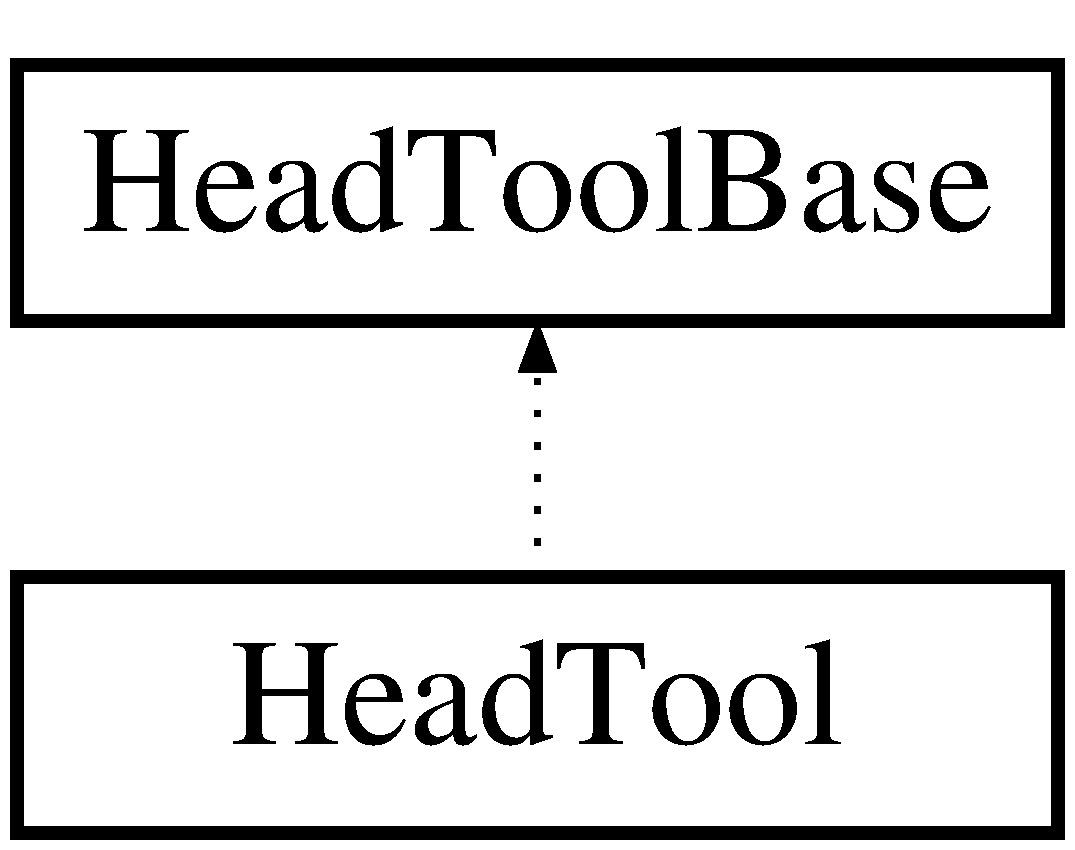
\includegraphics[height=2.000000cm]{d1/d4f/class_head_tool}
\end{center}
\end{figure}
\subsection*{Public Member Functions}
\begin{DoxyCompactItemize}
\item 
\hyperlink{class_head_tool_a9934c87c8f8eb515ff32e46c74004c0e}{Head\+Tool} (const double specific\+Gravity, const double flow\+Rate, const double suction\+Pipe\+Diameter, const double suction\+Gauge\+Pressure, const double suction\+Gauge\+Elevation, const double suction\+Line\+Loss\+Coefficients, const double discharge\+Pipe\+Diameter, const double discharge\+Gauge\+Pressure, const double discharge\+Gauge\+Elevation, const double discharge\+Line\+Loss\+Coefficients)
\item 
std\+::unordered\+\_\+map$<$ std\+::string, double $>$ \hyperlink{class_head_tool_ab107e7717df4ca95404ce1952c21a84e}{calculate} () override
\end{DoxyCompactItemize}


\subsection{Detailed Description}
Head Tool class Contains all of the properties of a head tool. Used to calculate all of the values of the returned unordered map. 

Definition at line 169 of file Head\+Tool.\+h.



\subsection{Constructor \& Destructor Documentation}
\mbox{\Hypertarget{class_head_tool_a9934c87c8f8eb515ff32e46c74004c0e}\label{class_head_tool_a9934c87c8f8eb515ff32e46c74004c0e}} 
\index{Head\+Tool@{Head\+Tool}!Head\+Tool@{Head\+Tool}}
\index{Head\+Tool@{Head\+Tool}!Head\+Tool@{Head\+Tool}}
\subsubsection{\texorpdfstring{Head\+Tool()}{HeadTool()}}
{\footnotesize\ttfamily Head\+Tool\+::\+Head\+Tool (\begin{DoxyParamCaption}\item[{const double}]{specific\+Gravity,  }\item[{const double}]{flow\+Rate,  }\item[{const double}]{suction\+Pipe\+Diameter,  }\item[{const double}]{suction\+Gauge\+Pressure,  }\item[{const double}]{suction\+Gauge\+Elevation,  }\item[{const double}]{suction\+Line\+Loss\+Coefficients,  }\item[{const double}]{discharge\+Pipe\+Diameter,  }\item[{const double}]{discharge\+Gauge\+Pressure,  }\item[{const double}]{discharge\+Gauge\+Elevation,  }\item[{const double}]{discharge\+Line\+Loss\+Coefficients }\end{DoxyParamCaption})\hspace{0.3cm}{\ttfamily [inline]}}

Constructor for \hyperlink{class_head_tool}{Head\+Tool} with no Suction Tank, all inputs specified


\begin{DoxyParams}{Parameters}
{\em specific\+Gravity} & double, specific gravity -\/ unitless \\
\hline
{\em flow\+Rate} & double, flow rate in gpm (gallons per minute) \\
\hline
{\em suction\+Pipe\+Diameter} & double, diameter of suction pipe in feet \\
\hline
{\em suction\+Gauge\+Pressure} & double, gauge pressure of suction in psig (pounds per square inch guage) \\
\hline
{\em suction\+Gauge\+Elevation} & double, gauge elevation of suction in feet \\
\hline
{\em suction\+Line\+Loss\+Coefficients} & double, line loss coefficients of suction -\/ unitless \\
\hline
{\em discharge\+Pipe\+Diameter} & double, diameter of discharge pipe in feet \\
\hline
{\em discharge\+Gauge\+Pressure} & double, gauge pressure of discharge in psig (pounds per square inch guage) \\
\hline
{\em discharge\+Gauge\+Elevation} & double, gauge elevation of discharge in feet \\
\hline
{\em discharge\+Line\+Loss\+Coefficients} & double, line loss coefficients of discharge -\/ unitless \\
\hline
\end{DoxyParams}


Definition at line 188 of file Head\+Tool.\+h.



\subsection{Member Function Documentation}
\mbox{\Hypertarget{class_head_tool_ab107e7717df4ca95404ce1952c21a84e}\label{class_head_tool_ab107e7717df4ca95404ce1952c21a84e}} 
\index{Head\+Tool@{Head\+Tool}!calculate@{calculate}}
\index{calculate@{calculate}!Head\+Tool@{Head\+Tool}}
\subsubsection{\texorpdfstring{calculate()}{calculate()}}
{\footnotesize\ttfamily std\+::unordered\+\_\+map$<$ std\+::string, double $>$ Head\+Tool\+::calculate (\begin{DoxyParamCaption}{ }\end{DoxyParamCaption})\hspace{0.3cm}{\ttfamily [override]}, {\ttfamily [virtual]}}

Calculates the operating pump head

\begin{DoxyReturn}{Returns}
unordered\+\_\+map with internal values calculated 
\end{DoxyReturn}


Implements \hyperlink{class_head_tool_base_ab8df8f908827ce45dc5e769ea0e10f0b}{Head\+Tool\+Base}.



Definition at line 50 of file Head\+Tool.\+cpp.



The documentation for this class was generated from the following files\+:\begin{DoxyCompactItemize}
\item 
include/calculator/pump/Head\+Tool.\+h\item 
src/calculator/pump/Head\+Tool.\+cpp\end{DoxyCompactItemize}

\hypertarget{class_head_tool_base}{}\section{Head\+Tool\+Base Class Reference}
\label{class_head_tool_base}\index{Head\+Tool\+Base@{Head\+Tool\+Base}}


Contains the entire hierarchy of the \hyperlink{class_head_tool}{Head\+Tool} classes. \hyperlink{class_head_tool_base_ab8df8f908827ce45dc5e769ea0e10f0b}{calculate()}\+: Calculates the operating pump head.  




{\ttfamily \#include $<$Head\+Tool.\+h$>$}

Inheritance diagram for Head\+Tool\+Base\+:\begin{figure}[H]
\begin{center}
\leavevmode
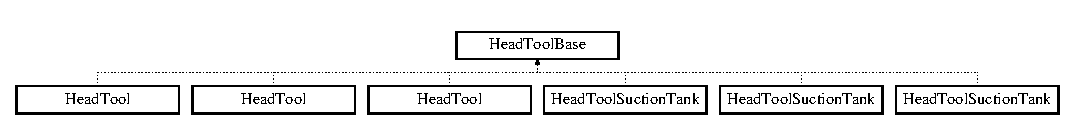
\includegraphics[height=2.000000cm]{d5/dc5/class_head_tool_base}
\end{center}
\end{figure}
\subsection*{Protected Member Functions}
\begin{DoxyCompactItemize}
\item 
\hyperlink{class_head_tool_base_ae5bb2325e1266c64b16937d964aea14f}{Head\+Tool\+Base} (const double specific\+Gravity, const double flow\+Rate, const double suction\+Pipe\+Diameter, const double suction\+Line\+Loss\+Coefficients, const double discharge\+Pipe\+Diameter, const double discharge\+Gauge\+Pressure, const double discharge\+Gauge\+Elevation, const double discharge\+Line\+Loss\+Coefficients)
\item 
virtual std\+::unordered\+\_\+map$<$ std\+::string, double $>$ \hyperlink{class_head_tool_base_ab8df8f908827ce45dc5e769ea0e10f0b}{calculate} ()=0
\item 
double \hyperlink{class_head_tool_base_ab79bb695c514b740d9ea01df60b68a23}{velocity} (const double diameter, const double flow)
\begin{DoxyCompactList}\small\item\em Contains the implementations of the \hyperlink{class_head_tool}{Head\+Tool} hierarchy methods. \hyperlink{class_head_tool_base_ab8df8f908827ce45dc5e769ea0e10f0b}{calculate()}\+: Calculates the operating pump head. \end{DoxyCompactList}\item 
double \hyperlink{class_head_tool_base_a1dbece05fc1a248fa2aa64b6f09602f6}{velocity\+Head} (const double \hyperlink{class_head_tool_base_ab79bb695c514b740d9ea01df60b68a23}{velocity}, const double gravity)
\end{DoxyCompactItemize}
\subsection*{Protected Attributes}
\begin{DoxyCompactItemize}
\item 
\mbox{\Hypertarget{class_head_tool_base_a19ee231d55b1bee31d48876e43da14de}\label{class_head_tool_base_a19ee231d55b1bee31d48876e43da14de}} 
const double \hyperlink{class_head_tool_base_a19ee231d55b1bee31d48876e43da14de}{specific\+Gravity\+\_\+}
\begin{DoxyCompactList}\small\item\em specific gravity -\/ unitless \end{DoxyCompactList}\item 
\mbox{\Hypertarget{class_head_tool_base_a5a52095ea100a279d48dfd97032d4658}\label{class_head_tool_base_a5a52095ea100a279d48dfd97032d4658}} 
const double \hyperlink{class_head_tool_base_a5a52095ea100a279d48dfd97032d4658}{flow\+Rate\+\_\+}
\begin{DoxyCompactList}\small\item\em flow rate in gpm \end{DoxyCompactList}\item 
\mbox{\Hypertarget{class_head_tool_base_a96fe7fbe12c4c0ac2cc6a0f681ffc170}\label{class_head_tool_base_a96fe7fbe12c4c0ac2cc6a0f681ffc170}} 
const double \hyperlink{class_head_tool_base_a96fe7fbe12c4c0ac2cc6a0f681ffc170}{suction\+Pipe\+Diameter\+\_\+}
\begin{DoxyCompactList}\small\item\em suction pipe diamter in inches \end{DoxyCompactList}\item 
\mbox{\Hypertarget{class_head_tool_base_a8cfbb2d33b36164e5be8f5ee785e62ea}\label{class_head_tool_base_a8cfbb2d33b36164e5be8f5ee785e62ea}} 
const double \hyperlink{class_head_tool_base_a8cfbb2d33b36164e5be8f5ee785e62ea}{suction\+Line\+Loss\+Coefficients\+\_\+}
\begin{DoxyCompactList}\small\item\em suction line loss coefficient -\/ unitless \end{DoxyCompactList}\item 
\mbox{\Hypertarget{class_head_tool_base_a34385a58538b690611f6f4fd11623c7f}\label{class_head_tool_base_a34385a58538b690611f6f4fd11623c7f}} 
const double \hyperlink{class_head_tool_base_a34385a58538b690611f6f4fd11623c7f}{discharge\+Pipe\+Diameter\+\_\+}
\begin{DoxyCompactList}\small\item\em discharge pipe diameter in inches \end{DoxyCompactList}\item 
\mbox{\Hypertarget{class_head_tool_base_a52413462e822c4cfdc77f19671216116}\label{class_head_tool_base_a52413462e822c4cfdc77f19671216116}} 
const double \hyperlink{class_head_tool_base_a52413462e822c4cfdc77f19671216116}{discharge\+Gauge\+Pressure\+\_\+}
\begin{DoxyCompactList}\small\item\em discharge gauge pressure in psi \end{DoxyCompactList}\item 
\mbox{\Hypertarget{class_head_tool_base_af4e7ff936d367e96119b4a976ce2740f}\label{class_head_tool_base_af4e7ff936d367e96119b4a976ce2740f}} 
const double \hyperlink{class_head_tool_base_af4e7ff936d367e96119b4a976ce2740f}{discharge\+Gauge\+Elevation\+\_\+}
\begin{DoxyCompactList}\small\item\em discharge gauge elevation in ft \end{DoxyCompactList}\item 
\mbox{\Hypertarget{class_head_tool_base_a02e59b19839499f82973a4b59690d5bd}\label{class_head_tool_base_a02e59b19839499f82973a4b59690d5bd}} 
const double \hyperlink{class_head_tool_base_a02e59b19839499f82973a4b59690d5bd}{discharge\+Line\+Loss\+Coefficients\+\_\+}
\begin{DoxyCompactList}\small\item\em discharge line loss coefficients -\/ unitless \end{DoxyCompactList}\item 
\mbox{\Hypertarget{class_head_tool_base_a106ba169bf4e10b7442659108f619209}\label{class_head_tool_base_a106ba169bf4e10b7442659108f619209}} 
const double \hyperlink{class_head_tool_base_a106ba169bf4e10b7442659108f619209}{gravity\+\_\+} = 32.\+1740
\begin{DoxyCompactList}\small\item\em gravity constant \end{DoxyCompactList}\item 
\mbox{\Hypertarget{class_head_tool_base_aa988ceec07264b1865d5d708b97b7450}\label{class_head_tool_base_aa988ceec07264b1865d5d708b97b7450}} 
const double \hyperlink{class_head_tool_base_aa988ceec07264b1865d5d708b97b7450}{P\+I\+\_\+} = 3.\+141592653589793238463
\begin{DoxyCompactList}\small\item\em value of Pi \end{DoxyCompactList}\end{DoxyCompactItemize}


\subsection{Detailed Description}
Contains the entire hierarchy of the \hyperlink{class_head_tool}{Head\+Tool} classes. \hyperlink{class_head_tool_base_ab8df8f908827ce45dc5e769ea0e10f0b}{calculate()}\+: Calculates the operating pump head. 

\begin{DoxyAuthor}{Author}
Preston Shires (pshires) 
\end{DoxyAuthor}
Head Tool Base class Contains all of the basic properties of a head tool. Used to calculate velocity and velocity head so those values can be used in the \hyperlink{class_head_tool_suction_tank}{Head\+Tool\+Suction\+Tank} class or \hyperlink{class_head_tool}{Head\+Tool} class to calculate all of the values in the returned map. 

Definition at line 21 of file Head\+Tool.\+h.



\subsection{Constructor \& Destructor Documentation}
\mbox{\Hypertarget{class_head_tool_base_ae5bb2325e1266c64b16937d964aea14f}\label{class_head_tool_base_ae5bb2325e1266c64b16937d964aea14f}} 
\index{Head\+Tool\+Base@{Head\+Tool\+Base}!Head\+Tool\+Base@{Head\+Tool\+Base}}
\index{Head\+Tool\+Base@{Head\+Tool\+Base}!Head\+Tool\+Base@{Head\+Tool\+Base}}
\subsubsection{\texorpdfstring{Head\+Tool\+Base()}{HeadToolBase()}}
{\footnotesize\ttfamily Head\+Tool\+Base\+::\+Head\+Tool\+Base (\begin{DoxyParamCaption}\item[{const double}]{specific\+Gravity,  }\item[{const double}]{flow\+Rate,  }\item[{const double}]{suction\+Pipe\+Diameter,  }\item[{const double}]{suction\+Line\+Loss\+Coefficients,  }\item[{const double}]{discharge\+Pipe\+Diameter,  }\item[{const double}]{discharge\+Gauge\+Pressure,  }\item[{const double}]{discharge\+Gauge\+Elevation,  }\item[{const double}]{discharge\+Line\+Loss\+Coefficients }\end{DoxyParamCaption})\hspace{0.3cm}{\ttfamily [inline]}, {\ttfamily [protected]}}

Constructor for the abstract \hyperlink{class_head_tool_base}{Head\+Tool\+Base} class with all inputs specified


\begin{DoxyParams}{Parameters}
{\em specific\+Gravity} & double, specific gravity -\/ unitless \\
\hline
{\em flow\+Rate} & double, flow rate in gpm (gallons per minute) \\
\hline
{\em suction\+Pipe\+Diameter} & double, diameter of suction pipe in inches \\
\hline
{\em suction\+Line\+Loss\+Coefficients} & double, suction line loss coefficient -\/ unitless \\
\hline
{\em discharge\+Pipe\+Diameter} & double, diameter of discharge pipe in inches \\
\hline
{\em discharge\+Gauge\+Pressure} & double, gauge pressure of discharge in psig (pounds per square inch gauge) \\
\hline
{\em discharge\+Gauge\+Elevation} & double, gauge elevation of discharge in feet \\
\hline
{\em discharge\+Line\+Loss\+Coefficients} & double, line loss coefficients of discharge -\/ unitless \\
\hline
\end{DoxyParams}


Definition at line 37 of file Head\+Tool.\+h.



\subsection{Member Function Documentation}
\mbox{\Hypertarget{class_head_tool_base_ab8df8f908827ce45dc5e769ea0e10f0b}\label{class_head_tool_base_ab8df8f908827ce45dc5e769ea0e10f0b}} 
\index{Head\+Tool\+Base@{Head\+Tool\+Base}!calculate@{calculate}}
\index{calculate@{calculate}!Head\+Tool\+Base@{Head\+Tool\+Base}}
\subsubsection{\texorpdfstring{calculate()}{calculate()}}
{\footnotesize\ttfamily virtual std\+::unordered\+\_\+map$<$std\+::string, double$>$ Head\+Tool\+Base\+::calculate (\begin{DoxyParamCaption}{ }\end{DoxyParamCaption})\hspace{0.3cm}{\ttfamily [protected]}, {\ttfamily [pure virtual]}}

Calculates the operating pump head

\begin{DoxyReturn}{Returns}
unordered map with all its values calculated 
\end{DoxyReturn}


Implemented in \hyperlink{class_head_tool_ab107e7717df4ca95404ce1952c21a84e}{Head\+Tool}, and \hyperlink{class_head_tool_suction_tank_a390a38466222aa3b87d2cf2ec84537a5}{Head\+Tool\+Suction\+Tank}.

\mbox{\Hypertarget{class_head_tool_base_ab79bb695c514b740d9ea01df60b68a23}\label{class_head_tool_base_ab79bb695c514b740d9ea01df60b68a23}} 
\index{Head\+Tool\+Base@{Head\+Tool\+Base}!velocity@{velocity}}
\index{velocity@{velocity}!Head\+Tool\+Base@{Head\+Tool\+Base}}
\subsubsection{\texorpdfstring{velocity()}{velocity()}}
{\footnotesize\ttfamily double Head\+Tool\+Base\+::velocity (\begin{DoxyParamCaption}\item[{const double}]{diameter,  }\item[{const double}]{flow }\end{DoxyParamCaption})\hspace{0.3cm}{\ttfamily [protected]}}



Contains the implementations of the \hyperlink{class_head_tool}{Head\+Tool} hierarchy methods. \hyperlink{class_head_tool_base_ab8df8f908827ce45dc5e769ea0e10f0b}{calculate()}\+: Calculates the operating pump head. 

Calculates the velocity


\begin{DoxyParams}{Parameters}
{\em diameter} & const double, diameter in inches \\
\hline
{\em flow} & const double, flow rate in gpm\\
\hline
\end{DoxyParams}
\begin{DoxyReturn}{Returns}
double, velocity in ft/s
\end{DoxyReturn}
\begin{DoxyAuthor}{Author}
Preston Shires (pshires) 
\end{DoxyAuthor}


Definition at line 12 of file Head\+Tool.\+cpp.

\mbox{\Hypertarget{class_head_tool_base_a1dbece05fc1a248fa2aa64b6f09602f6}\label{class_head_tool_base_a1dbece05fc1a248fa2aa64b6f09602f6}} 
\index{Head\+Tool\+Base@{Head\+Tool\+Base}!velocity\+Head@{velocity\+Head}}
\index{velocity\+Head@{velocity\+Head}!Head\+Tool\+Base@{Head\+Tool\+Base}}
\subsubsection{\texorpdfstring{velocity\+Head()}{velocityHead()}}
{\footnotesize\ttfamily double Head\+Tool\+Base\+::velocity\+Head (\begin{DoxyParamCaption}\item[{const double}]{velocity,  }\item[{const double}]{gravity }\end{DoxyParamCaption})\hspace{0.3cm}{\ttfamily [protected]}}

Calculates the velocity head


\begin{DoxyParams}{Parameters}
{\em velocity} & const double, velocity in ft/s \\
\hline
{\em gravity} & const double, gravity in ft/s$^\wedge$2 \\
\hline
\end{DoxyParams}


Definition at line 16 of file Head\+Tool.\+cpp.



The documentation for this class was generated from the following files\+:\begin{DoxyCompactItemize}
\item 
include/calculator/pump/Head\+Tool.\+h\item 
src/calculator/pump/Head\+Tool.\+cpp\end{DoxyCompactItemize}

\hypertarget{class_head_tool_suction_tank}{}\section{Head\+Tool\+Suction\+Tank Class Reference}
\label{class_head_tool_suction_tank}\index{Head\+Tool\+Suction\+Tank@{Head\+Tool\+Suction\+Tank}}


{\ttfamily \#include $<$Head\+Tool.\+h$>$}

Inheritance diagram for Head\+Tool\+Suction\+Tank\+:\begin{figure}[H]
\begin{center}
\leavevmode
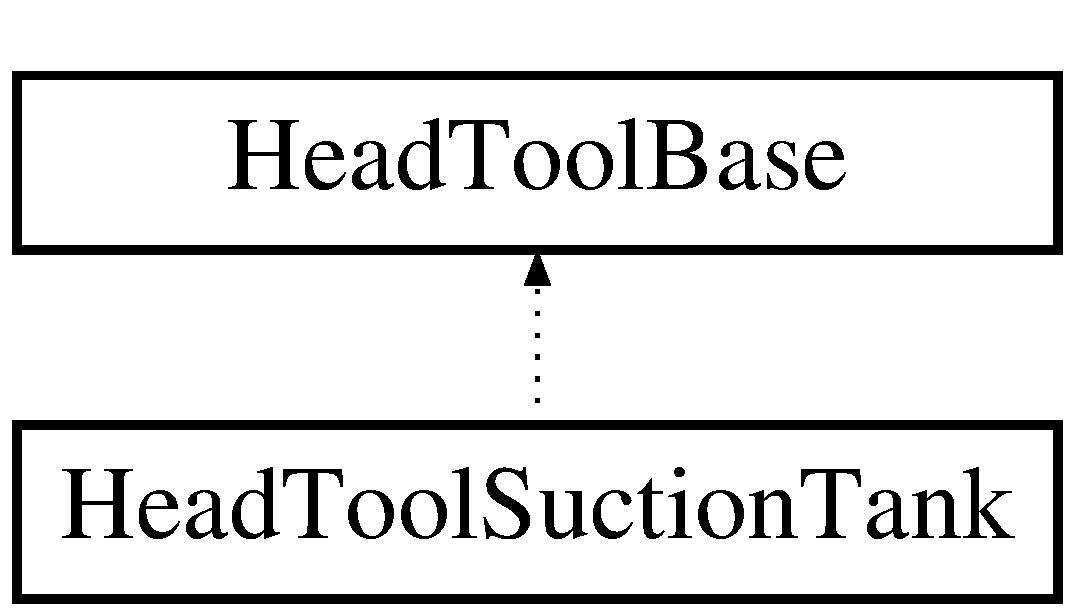
\includegraphics[height=2.000000cm]{d8/dec/class_head_tool_suction_tank}
\end{center}
\end{figure}
\subsection*{Public Member Functions}
\begin{DoxyCompactItemize}
\item 
\hyperlink{class_head_tool_suction_tank_a96579ecd414c723362db00cfeb24cd46}{Head\+Tool\+Suction\+Tank} (const double specific\+Gravity, const double flow\+Rate, const double suction\+Pipe\+Diameter, const double suction\+Tank\+Gas\+Over\+Pressure, const double suction\+Tank\+Fluid\+Surface\+Elevation, const double suction\+Line\+Loss\+Coefficients, const double discharge\+Pipe\+Diameter, const double discharge\+Gauge\+Pressure, const double discharge\+Gauge\+Elevation, const double discharge\+Line\+Loss\+Coefficients)
\item 
std\+::unordered\+\_\+map$<$ std\+::string, double $>$ \hyperlink{class_head_tool_suction_tank_a390a38466222aa3b87d2cf2ec84537a5}{calculate} () override
\end{DoxyCompactItemize}


\subsection{Detailed Description}
Head Tool Suction Tank class Contains all of the properties of a head tool suction tank. Used to calculate all of the values in the returned map. 

Definition at line 110 of file Head\+Tool.\+h.



\subsection{Constructor \& Destructor Documentation}
\mbox{\Hypertarget{class_head_tool_suction_tank_a96579ecd414c723362db00cfeb24cd46}\label{class_head_tool_suction_tank_a96579ecd414c723362db00cfeb24cd46}} 
\index{Head\+Tool\+Suction\+Tank@{Head\+Tool\+Suction\+Tank}!Head\+Tool\+Suction\+Tank@{Head\+Tool\+Suction\+Tank}}
\index{Head\+Tool\+Suction\+Tank@{Head\+Tool\+Suction\+Tank}!Head\+Tool\+Suction\+Tank@{Head\+Tool\+Suction\+Tank}}
\subsubsection{\texorpdfstring{Head\+Tool\+Suction\+Tank()}{HeadToolSuctionTank()}}
{\footnotesize\ttfamily Head\+Tool\+Suction\+Tank\+::\+Head\+Tool\+Suction\+Tank (\begin{DoxyParamCaption}\item[{const double}]{specific\+Gravity,  }\item[{const double}]{flow\+Rate,  }\item[{const double}]{suction\+Pipe\+Diameter,  }\item[{const double}]{suction\+Tank\+Gas\+Over\+Pressure,  }\item[{const double}]{suction\+Tank\+Fluid\+Surface\+Elevation,  }\item[{const double}]{suction\+Line\+Loss\+Coefficients,  }\item[{const double}]{discharge\+Pipe\+Diameter,  }\item[{const double}]{discharge\+Gauge\+Pressure,  }\item[{const double}]{discharge\+Gauge\+Elevation,  }\item[{const double}]{discharge\+Line\+Loss\+Coefficients }\end{DoxyParamCaption})\hspace{0.3cm}{\ttfamily [inline]}}

Constructor for the \hyperlink{class_head_tool_suction_tank}{Head\+Tool\+Suction\+Tank} class with all inputs specified


\begin{DoxyParams}{Parameters}
{\em specific\+Gravity} & double, specific gravity -\/ unitless \\
\hline
{\em flow\+Rate} & double, flow rate in gpm (gallons per minute) \\
\hline
{\em suction\+Pipe\+Diameter} & double, diameter of suction pipe in feet \\
\hline
{\em suction\+Tank\+Gas\+Over\+Pressure} & double, gas over pressure of suction tank in psig (pounds per square inch gauage) \\
\hline
{\em suction\+Tank\+Fluid\+Surface\+Elevation} & double, fluid surface elevation of suction tank in feet \\
\hline
{\em suction\+Line\+Loss\+Coefficients} & double, line loss coefficients of suction -\/ unitless \\
\hline
{\em discharge\+Pipe\+Diameter} & double, diameter of discharge pipe in feet \\
\hline
{\em discharge\+Gauge\+Pressure} & double, gauge pressure of discharge in psig (pounds per square inch gauge) \\
\hline
{\em discharge\+Gauge\+Elevation} & double, gauge elevation of discharge in inches \\
\hline
{\em discharge\+Line\+Loss\+Coefficients} & double, line loss coefficients of discharge -\/ unitless \\
\hline
\end{DoxyParams}


Definition at line 129 of file Head\+Tool.\+h.



\subsection{Member Function Documentation}
\mbox{\Hypertarget{class_head_tool_suction_tank_a390a38466222aa3b87d2cf2ec84537a5}\label{class_head_tool_suction_tank_a390a38466222aa3b87d2cf2ec84537a5}} 
\index{Head\+Tool\+Suction\+Tank@{Head\+Tool\+Suction\+Tank}!calculate@{calculate}}
\index{calculate@{calculate}!Head\+Tool\+Suction\+Tank@{Head\+Tool\+Suction\+Tank}}
\subsubsection{\texorpdfstring{calculate()}{calculate()}}
{\footnotesize\ttfamily std\+::unordered\+\_\+map$<$ std\+::string, double $>$ Head\+Tool\+Suction\+Tank\+::calculate (\begin{DoxyParamCaption}{ }\end{DoxyParamCaption})\hspace{0.3cm}{\ttfamily [override]}, {\ttfamily [virtual]}}

Calculates the operating pump head

\begin{DoxyReturn}{Returns}
unordered map with all the values calculated for operating pump head 
\end{DoxyReturn}


Implements \hyperlink{class_head_tool_base_ab8df8f908827ce45dc5e769ea0e10f0b}{Head\+Tool\+Base}.



Definition at line 20 of file Head\+Tool.\+cpp.



The documentation for this class was generated from the following files\+:\begin{DoxyCompactItemize}
\item 
include/calculator/pump/Head\+Tool.\+h\item 
src/calculator/pump/Head\+Tool.\+cpp\end{DoxyCompactItemize}

\hypertarget{class_heat_loss}{}\section{Heat\+Loss Class Reference}
\label{class_heat_loss}\index{Heat\+Loss@{Heat\+Loss}}


{\ttfamily \#include $<$Heat\+Loss.\+h$>$}

\subsection*{Public Member Functions}
\begin{DoxyCompactItemize}
\item 
\hyperlink{class_heat_loss_a1c1bba4ef783d97e2ed63f39f625e82f}{Heat\+Loss} (double inlet\+Pressure, \hyperlink{class_steam_properties_ae0294bedf7d178c2d8fb6aed0f62fbff}{Steam\+Properties\+::\+Thermodynamic\+Quantity} quantity\+Type, double quantity\+Value, double inlet\+Mass\+Flow, double percent\+Heat\+Loss)
\item 
\hyperlink{struct_steam_system_modeler_tool_1_1_fluid_properties}{Steam\+System\+Modeler\+Tool\+::\+Fluid\+Properties} const  \& \hyperlink{class_heat_loss_a7bea461460dbacf1855d5375bbf6c097}{get\+Inlet\+Properties} () const
\item 
\hyperlink{struct_steam_system_modeler_tool_1_1_fluid_properties}{Steam\+System\+Modeler\+Tool\+::\+Fluid\+Properties} const  \& \hyperlink{class_heat_loss_a3e483dda6f393d67d7a0f28bcd75e545}{get\+Outlet\+Properties} () const
\item 
double \hyperlink{class_heat_loss_acc39533782f4f5cbf902d36f7bfc53b0}{get\+Heat\+Loss} () const
\item 
double \hyperlink{class_heat_loss_a09e6e05477fd6794ea7f42bb43da2f50}{get\+Inlet\+Pressure} () const
\item 
double \hyperlink{class_heat_loss_a7f7fd85e4fc8bf96dcc213f3dd44ecf7}{get\+Quantity\+Value} () const
\item 
double \hyperlink{class_heat_loss_ad11a428f99a4945628f66adecb88bf5a}{get\+Inlet\+Mass\+Flow} () const
\item 
double \hyperlink{class_heat_loss_acbbf01db5cde157057e4d766cab22382}{get\+Percent\+Heat\+Loss} () const
\item 
\hyperlink{class_steam_properties_ae0294bedf7d178c2d8fb6aed0f62fbff}{Steam\+Properties\+::\+Thermodynamic\+Quantity} \hyperlink{class_heat_loss_a92dc973c0fd81df192207b3df55d6c2b}{get\+Quantity\+Type} () const
\item 
void \hyperlink{class_heat_loss_ab0a6b1f2a964d161d25758318f25f7e3}{set\+Inlet\+Pressure} (double inlet\+Pressure)
\item 
void \hyperlink{class_heat_loss_ae6b6c4ac28471d7bc94e3886c48a90bd}{set\+Quantity\+Value} (double quantity\+Value)
\item 
void \hyperlink{class_heat_loss_ac4154dc9922b6ddf3f2e7a10cc64c61f}{set\+Inlet\+Mass\+Flow} (double inlet\+Mass\+Flow)
\item 
void \hyperlink{class_heat_loss_a2a4a80b16c1f975e194ae466b20d46bd}{set\+Percent\+Heat\+Loss} (double percent\+Heat\+Loss)
\item 
void \hyperlink{class_heat_loss_a7c125f1137f31eba8826a1aa3b905290}{set\+Quantity\+Type} (\hyperlink{class_steam_properties_ae0294bedf7d178c2d8fb6aed0f62fbff}{Steam\+Properties\+::\+Thermodynamic\+Quantity} quantity\+Type)
\item 
\hyperlink{class_heat_loss_a1c1bba4ef783d97e2ed63f39f625e82f}{Heat\+Loss} (double inlet\+Pressure, \hyperlink{class_steam_properties_ae0294bedf7d178c2d8fb6aed0f62fbff}{Steam\+Properties\+::\+Thermodynamic\+Quantity} quantity\+Type, double quantity\+Value, double inlet\+Mass\+Flow, double percent\+Heat\+Loss)
\item 
\hyperlink{struct_steam_system_modeler_tool_1_1_fluid_properties}{Steam\+System\+Modeler\+Tool\+::\+Fluid\+Properties} const  \& \hyperlink{class_heat_loss_a7bea461460dbacf1855d5375bbf6c097}{get\+Inlet\+Properties} () const
\item 
\hyperlink{struct_steam_system_modeler_tool_1_1_fluid_properties}{Steam\+System\+Modeler\+Tool\+::\+Fluid\+Properties} const  \& \hyperlink{class_heat_loss_a3e483dda6f393d67d7a0f28bcd75e545}{get\+Outlet\+Properties} () const
\item 
double \hyperlink{class_heat_loss_acc39533782f4f5cbf902d36f7bfc53b0}{get\+Heat\+Loss} () const
\item 
double \hyperlink{class_heat_loss_a09e6e05477fd6794ea7f42bb43da2f50}{get\+Inlet\+Pressure} () const
\item 
double \hyperlink{class_heat_loss_a7f7fd85e4fc8bf96dcc213f3dd44ecf7}{get\+Quantity\+Value} () const
\item 
double \hyperlink{class_heat_loss_ad11a428f99a4945628f66adecb88bf5a}{get\+Inlet\+Mass\+Flow} () const
\item 
double \hyperlink{class_heat_loss_acbbf01db5cde157057e4d766cab22382}{get\+Percent\+Heat\+Loss} () const
\item 
\hyperlink{class_steam_properties_ae0294bedf7d178c2d8fb6aed0f62fbff}{Steam\+Properties\+::\+Thermodynamic\+Quantity} \hyperlink{class_heat_loss_a92dc973c0fd81df192207b3df55d6c2b}{get\+Quantity\+Type} () const
\item 
void \hyperlink{class_heat_loss_ab0a6b1f2a964d161d25758318f25f7e3}{set\+Inlet\+Pressure} (double inlet\+Pressure)
\item 
void \hyperlink{class_heat_loss_ae6b6c4ac28471d7bc94e3886c48a90bd}{set\+Quantity\+Value} (double quantity\+Value)
\item 
void \hyperlink{class_heat_loss_ac4154dc9922b6ddf3f2e7a10cc64c61f}{set\+Inlet\+Mass\+Flow} (double inlet\+Mass\+Flow)
\item 
void \hyperlink{class_heat_loss_a2a4a80b16c1f975e194ae466b20d46bd}{set\+Percent\+Heat\+Loss} (double percent\+Heat\+Loss)
\item 
void \hyperlink{class_heat_loss_a7c125f1137f31eba8826a1aa3b905290}{set\+Quantity\+Type} (\hyperlink{class_steam_properties_ae0294bedf7d178c2d8fb6aed0f62fbff}{Steam\+Properties\+::\+Thermodynamic\+Quantity} quantity\+Type)
\item 
\hyperlink{class_heat_loss_a1c1bba4ef783d97e2ed63f39f625e82f}{Heat\+Loss} (double inlet\+Pressure, \hyperlink{class_steam_properties_ae0294bedf7d178c2d8fb6aed0f62fbff}{Steam\+Properties\+::\+Thermodynamic\+Quantity} quantity\+Type, double quantity\+Value, double inlet\+Mass\+Flow, double percent\+Heat\+Loss)
\item 
\hyperlink{struct_steam_system_modeler_tool_1_1_fluid_properties}{Steam\+System\+Modeler\+Tool\+::\+Fluid\+Properties} const  \& \hyperlink{class_heat_loss_a7bea461460dbacf1855d5375bbf6c097}{get\+Inlet\+Properties} () const
\item 
\hyperlink{struct_steam_system_modeler_tool_1_1_fluid_properties}{Steam\+System\+Modeler\+Tool\+::\+Fluid\+Properties} const  \& \hyperlink{class_heat_loss_a3e483dda6f393d67d7a0f28bcd75e545}{get\+Outlet\+Properties} () const
\item 
double \hyperlink{class_heat_loss_acc39533782f4f5cbf902d36f7bfc53b0}{get\+Heat\+Loss} () const
\item 
double \hyperlink{class_heat_loss_a09e6e05477fd6794ea7f42bb43da2f50}{get\+Inlet\+Pressure} () const
\item 
double \hyperlink{class_heat_loss_a7f7fd85e4fc8bf96dcc213f3dd44ecf7}{get\+Quantity\+Value} () const
\item 
double \hyperlink{class_heat_loss_ad11a428f99a4945628f66adecb88bf5a}{get\+Inlet\+Mass\+Flow} () const
\item 
double \hyperlink{class_heat_loss_acbbf01db5cde157057e4d766cab22382}{get\+Percent\+Heat\+Loss} () const
\item 
\hyperlink{class_steam_properties_ae0294bedf7d178c2d8fb6aed0f62fbff}{Steam\+Properties\+::\+Thermodynamic\+Quantity} \hyperlink{class_heat_loss_a92dc973c0fd81df192207b3df55d6c2b}{get\+Quantity\+Type} () const
\item 
void \hyperlink{class_heat_loss_ab0a6b1f2a964d161d25758318f25f7e3}{set\+Inlet\+Pressure} (double inlet\+Pressure)
\item 
void \hyperlink{class_heat_loss_ae6b6c4ac28471d7bc94e3886c48a90bd}{set\+Quantity\+Value} (double quantity\+Value)
\item 
void \hyperlink{class_heat_loss_ac4154dc9922b6ddf3f2e7a10cc64c61f}{set\+Inlet\+Mass\+Flow} (double inlet\+Mass\+Flow)
\item 
void \hyperlink{class_heat_loss_a2a4a80b16c1f975e194ae466b20d46bd}{set\+Percent\+Heat\+Loss} (double percent\+Heat\+Loss)
\item 
void \hyperlink{class_heat_loss_a7c125f1137f31eba8826a1aa3b905290}{set\+Quantity\+Type} (\hyperlink{class_steam_properties_ae0294bedf7d178c2d8fb6aed0f62fbff}{Steam\+Properties\+::\+Thermodynamic\+Quantity} quantity\+Type)
\end{DoxyCompactItemize}


\subsection{Detailed Description}
Heat Loss calculator class Used to calculate the heat energy loss and outlet steam properties 

Definition at line 22 of file Heat\+Loss.\+h.



\subsection{Constructor \& Destructor Documentation}
\mbox{\Hypertarget{class_heat_loss_a1c1bba4ef783d97e2ed63f39f625e82f}\label{class_heat_loss_a1c1bba4ef783d97e2ed63f39f625e82f}} 
\index{Heat\+Loss@{Heat\+Loss}!Heat\+Loss@{Heat\+Loss}}
\index{Heat\+Loss@{Heat\+Loss}!Heat\+Loss@{Heat\+Loss}}
\subsubsection{\texorpdfstring{Heat\+Loss()}{HeatLoss()}\hspace{0.1cm}{\footnotesize\ttfamily [1/3]}}
{\footnotesize\ttfamily Heat\+Loss\+::\+Heat\+Loss (\begin{DoxyParamCaption}\item[{double}]{inlet\+Pressure,  }\item[{\hyperlink{class_steam_properties_ae0294bedf7d178c2d8fb6aed0f62fbff}{Steam\+Properties\+::\+Thermodynamic\+Quantity}}]{quantity\+Type,  }\item[{double}]{quantity\+Value,  }\item[{double}]{inlet\+Mass\+Flow,  }\item[{double}]{percent\+Heat\+Loss }\end{DoxyParamCaption})}

Constructor for the heat loss calculator


\begin{DoxyParams}{Parameters}
{\em inlet\+Pressure} & double, inlet pressure in M\+Pa \\
\hline
{\em quantity\+Type} & \hyperlink{class_steam_properties_ae0294bedf7d178c2d8fb6aed0f62fbff}{Steam\+Properties\+::\+Thermodynamic\+Quantity}, type of quantity (either temperature in K, enthalpy in k\+J/kg, entropy in k\+J/kg/K, or quality -\/ unitless) \\
\hline
{\em quantity\+Value} & double, value of the quantity (either temperature in K, enthalpy in k\+J/kg, entropy in k\+J/kg/K, or quality -\/ unitless) \\
\hline
{\em inlet\+Mass\+Flow} & double, inlet mass flow in kg/hr \\
\hline
{\em percent\+Heat\+Loss} & double, heat loss as \% \\
\hline
\end{DoxyParams}


Definition at line 12 of file Heat\+Loss.\+cpp.

\mbox{\Hypertarget{class_heat_loss_a1c1bba4ef783d97e2ed63f39f625e82f}\label{class_heat_loss_a1c1bba4ef783d97e2ed63f39f625e82f}} 
\index{Heat\+Loss@{Heat\+Loss}!Heat\+Loss@{Heat\+Loss}}
\index{Heat\+Loss@{Heat\+Loss}!Heat\+Loss@{Heat\+Loss}}
\subsubsection{\texorpdfstring{Heat\+Loss()}{HeatLoss()}\hspace{0.1cm}{\footnotesize\ttfamily [2/3]}}
{\footnotesize\ttfamily Heat\+Loss\+::\+Heat\+Loss (\begin{DoxyParamCaption}\item[{double}]{inlet\+Pressure,  }\item[{\hyperlink{class_steam_properties_ae0294bedf7d178c2d8fb6aed0f62fbff}{Steam\+Properties\+::\+Thermodynamic\+Quantity}}]{quantity\+Type,  }\item[{double}]{quantity\+Value,  }\item[{double}]{inlet\+Mass\+Flow,  }\item[{double}]{percent\+Heat\+Loss }\end{DoxyParamCaption})}

Constructor for the heat loss calculator


\begin{DoxyParams}{Parameters}
{\em inlet\+Pressure} & double, inlet pressure in M\+Pa \\
\hline
{\em quantity\+Type} & \hyperlink{class_steam_properties_ae0294bedf7d178c2d8fb6aed0f62fbff}{Steam\+Properties\+::\+Thermodynamic\+Quantity}, type of quantity (either temperature in K, enthalpy in k\+J/kg, entropy in k\+J/kg/K, or quality -\/ unitless) \\
\hline
{\em quantity\+Value} & double, value of the quantity (either temperature in K, enthalpy in k\+J/kg, entropy in k\+J/kg/K, or quality -\/ unitless) \\
\hline
{\em inlet\+Mass\+Flow} & double, inlet mass flow in kg/hr \\
\hline
{\em percent\+Heat\+Loss} & double, heat loss as \% \\
\hline
\end{DoxyParams}
\mbox{\Hypertarget{class_heat_loss_a1c1bba4ef783d97e2ed63f39f625e82f}\label{class_heat_loss_a1c1bba4ef783d97e2ed63f39f625e82f}} 
\index{Heat\+Loss@{Heat\+Loss}!Heat\+Loss@{Heat\+Loss}}
\index{Heat\+Loss@{Heat\+Loss}!Heat\+Loss@{Heat\+Loss}}
\subsubsection{\texorpdfstring{Heat\+Loss()}{HeatLoss()}\hspace{0.1cm}{\footnotesize\ttfamily [3/3]}}
{\footnotesize\ttfamily Heat\+Loss\+::\+Heat\+Loss (\begin{DoxyParamCaption}\item[{double}]{inlet\+Pressure,  }\item[{\hyperlink{class_steam_properties_ae0294bedf7d178c2d8fb6aed0f62fbff}{Steam\+Properties\+::\+Thermodynamic\+Quantity}}]{quantity\+Type,  }\item[{double}]{quantity\+Value,  }\item[{double}]{inlet\+Mass\+Flow,  }\item[{double}]{percent\+Heat\+Loss }\end{DoxyParamCaption})}

Constructor for the heat loss calculator


\begin{DoxyParams}{Parameters}
{\em inlet\+Pressure} & double, inlet pressure in M\+Pa \\
\hline
{\em quantity\+Type} & \hyperlink{class_steam_properties_ae0294bedf7d178c2d8fb6aed0f62fbff}{Steam\+Properties\+::\+Thermodynamic\+Quantity}, type of quantity (either temperature in K, enthalpy in k\+J/kg, entropy in k\+J/kg/K, or quality -\/ unitless) \\
\hline
{\em quantity\+Value} & double, value of the quantity (either temperature in K, enthalpy in k\+J/kg, entropy in k\+J/kg/K, or quality -\/ unitless) \\
\hline
{\em inlet\+Mass\+Flow} & double, inlet mass flow in kg/hr \\
\hline
{\em percent\+Heat\+Loss} & double, heat loss as \% \\
\hline
\end{DoxyParams}


\subsection{Member Function Documentation}
\mbox{\Hypertarget{class_heat_loss_acc39533782f4f5cbf902d36f7bfc53b0}\label{class_heat_loss_acc39533782f4f5cbf902d36f7bfc53b0}} 
\index{Heat\+Loss@{Heat\+Loss}!get\+Heat\+Loss@{get\+Heat\+Loss}}
\index{get\+Heat\+Loss@{get\+Heat\+Loss}!Heat\+Loss@{Heat\+Loss}}
\subsubsection{\texorpdfstring{get\+Heat\+Loss()}{getHeatLoss()}\hspace{0.1cm}{\footnotesize\ttfamily [1/3]}}
{\footnotesize\ttfamily double Heat\+Loss\+::get\+Heat\+Loss (\begin{DoxyParamCaption}{ }\end{DoxyParamCaption}) const\hspace{0.3cm}{\ttfamily [inline]}}

Gets the heat loss \begin{DoxyReturn}{Returns}
double, heat loss in M\+J/hr 
\end{DoxyReturn}


Definition at line 53 of file Heat\+Loss.\+h.

\mbox{\Hypertarget{class_heat_loss_acc39533782f4f5cbf902d36f7bfc53b0}\label{class_heat_loss_acc39533782f4f5cbf902d36f7bfc53b0}} 
\index{Heat\+Loss@{Heat\+Loss}!get\+Heat\+Loss@{get\+Heat\+Loss}}
\index{get\+Heat\+Loss@{get\+Heat\+Loss}!Heat\+Loss@{Heat\+Loss}}
\subsubsection{\texorpdfstring{get\+Heat\+Loss()}{getHeatLoss()}\hspace{0.1cm}{\footnotesize\ttfamily [2/3]}}
{\footnotesize\ttfamily double Heat\+Loss\+::get\+Heat\+Loss (\begin{DoxyParamCaption}{ }\end{DoxyParamCaption}) const\hspace{0.3cm}{\ttfamily [inline]}}

Gets the heat loss \begin{DoxyReturn}{Returns}
double, heat loss in M\+J/hr 
\end{DoxyReturn}


Definition at line 53 of file Heat\+Loss.\+h.

\mbox{\Hypertarget{class_heat_loss_acc39533782f4f5cbf902d36f7bfc53b0}\label{class_heat_loss_acc39533782f4f5cbf902d36f7bfc53b0}} 
\index{Heat\+Loss@{Heat\+Loss}!get\+Heat\+Loss@{get\+Heat\+Loss}}
\index{get\+Heat\+Loss@{get\+Heat\+Loss}!Heat\+Loss@{Heat\+Loss}}
\subsubsection{\texorpdfstring{get\+Heat\+Loss()}{getHeatLoss()}\hspace{0.1cm}{\footnotesize\ttfamily [3/3]}}
{\footnotesize\ttfamily double Heat\+Loss\+::get\+Heat\+Loss (\begin{DoxyParamCaption}{ }\end{DoxyParamCaption}) const\hspace{0.3cm}{\ttfamily [inline]}}

Gets the heat loss \begin{DoxyReturn}{Returns}
double, heat loss in M\+J/hr 
\end{DoxyReturn}


Definition at line 53 of file Heat\+Loss.\+h.

\mbox{\Hypertarget{class_heat_loss_ad11a428f99a4945628f66adecb88bf5a}\label{class_heat_loss_ad11a428f99a4945628f66adecb88bf5a}} 
\index{Heat\+Loss@{Heat\+Loss}!get\+Inlet\+Mass\+Flow@{get\+Inlet\+Mass\+Flow}}
\index{get\+Inlet\+Mass\+Flow@{get\+Inlet\+Mass\+Flow}!Heat\+Loss@{Heat\+Loss}}
\subsubsection{\texorpdfstring{get\+Inlet\+Mass\+Flow()}{getInletMassFlow()}\hspace{0.1cm}{\footnotesize\ttfamily [1/3]}}
{\footnotesize\ttfamily double Heat\+Loss\+::get\+Inlet\+Mass\+Flow (\begin{DoxyParamCaption}{ }\end{DoxyParamCaption}) const\hspace{0.3cm}{\ttfamily [inline]}}

Gets the inlet mass flow \begin{DoxyReturn}{Returns}
double, mass flow of the inlet steam in kg/hr 
\end{DoxyReturn}


Definition at line 71 of file Heat\+Loss.\+h.

\mbox{\Hypertarget{class_heat_loss_ad11a428f99a4945628f66adecb88bf5a}\label{class_heat_loss_ad11a428f99a4945628f66adecb88bf5a}} 
\index{Heat\+Loss@{Heat\+Loss}!get\+Inlet\+Mass\+Flow@{get\+Inlet\+Mass\+Flow}}
\index{get\+Inlet\+Mass\+Flow@{get\+Inlet\+Mass\+Flow}!Heat\+Loss@{Heat\+Loss}}
\subsubsection{\texorpdfstring{get\+Inlet\+Mass\+Flow()}{getInletMassFlow()}\hspace{0.1cm}{\footnotesize\ttfamily [2/3]}}
{\footnotesize\ttfamily double Heat\+Loss\+::get\+Inlet\+Mass\+Flow (\begin{DoxyParamCaption}{ }\end{DoxyParamCaption}) const\hspace{0.3cm}{\ttfamily [inline]}}

Gets the inlet mass flow \begin{DoxyReturn}{Returns}
double, mass flow of the inlet steam in kg/hr 
\end{DoxyReturn}


Definition at line 71 of file Heat\+Loss.\+h.

\mbox{\Hypertarget{class_heat_loss_ad11a428f99a4945628f66adecb88bf5a}\label{class_heat_loss_ad11a428f99a4945628f66adecb88bf5a}} 
\index{Heat\+Loss@{Heat\+Loss}!get\+Inlet\+Mass\+Flow@{get\+Inlet\+Mass\+Flow}}
\index{get\+Inlet\+Mass\+Flow@{get\+Inlet\+Mass\+Flow}!Heat\+Loss@{Heat\+Loss}}
\subsubsection{\texorpdfstring{get\+Inlet\+Mass\+Flow()}{getInletMassFlow()}\hspace{0.1cm}{\footnotesize\ttfamily [3/3]}}
{\footnotesize\ttfamily double Heat\+Loss\+::get\+Inlet\+Mass\+Flow (\begin{DoxyParamCaption}{ }\end{DoxyParamCaption}) const\hspace{0.3cm}{\ttfamily [inline]}}

Gets the inlet mass flow \begin{DoxyReturn}{Returns}
double, mass flow of the inlet steam in kg/hr 
\end{DoxyReturn}


Definition at line 71 of file Heat\+Loss.\+h.

\mbox{\Hypertarget{class_heat_loss_a09e6e05477fd6794ea7f42bb43da2f50}\label{class_heat_loss_a09e6e05477fd6794ea7f42bb43da2f50}} 
\index{Heat\+Loss@{Heat\+Loss}!get\+Inlet\+Pressure@{get\+Inlet\+Pressure}}
\index{get\+Inlet\+Pressure@{get\+Inlet\+Pressure}!Heat\+Loss@{Heat\+Loss}}
\subsubsection{\texorpdfstring{get\+Inlet\+Pressure()}{getInletPressure()}\hspace{0.1cm}{\footnotesize\ttfamily [1/3]}}
{\footnotesize\ttfamily double Heat\+Loss\+::get\+Inlet\+Pressure (\begin{DoxyParamCaption}{ }\end{DoxyParamCaption}) const\hspace{0.3cm}{\ttfamily [inline]}}

Gets the inlet pressure \begin{DoxyReturn}{Returns}
double, pressure of the inlet steam in M\+Pa 
\end{DoxyReturn}


Definition at line 59 of file Heat\+Loss.\+h.

\mbox{\Hypertarget{class_heat_loss_a09e6e05477fd6794ea7f42bb43da2f50}\label{class_heat_loss_a09e6e05477fd6794ea7f42bb43da2f50}} 
\index{Heat\+Loss@{Heat\+Loss}!get\+Inlet\+Pressure@{get\+Inlet\+Pressure}}
\index{get\+Inlet\+Pressure@{get\+Inlet\+Pressure}!Heat\+Loss@{Heat\+Loss}}
\subsubsection{\texorpdfstring{get\+Inlet\+Pressure()}{getInletPressure()}\hspace{0.1cm}{\footnotesize\ttfamily [2/3]}}
{\footnotesize\ttfamily double Heat\+Loss\+::get\+Inlet\+Pressure (\begin{DoxyParamCaption}{ }\end{DoxyParamCaption}) const\hspace{0.3cm}{\ttfamily [inline]}}

Gets the inlet pressure \begin{DoxyReturn}{Returns}
double, pressure of the inlet steam in M\+Pa 
\end{DoxyReturn}


Definition at line 59 of file Heat\+Loss.\+h.

\mbox{\Hypertarget{class_heat_loss_a09e6e05477fd6794ea7f42bb43da2f50}\label{class_heat_loss_a09e6e05477fd6794ea7f42bb43da2f50}} 
\index{Heat\+Loss@{Heat\+Loss}!get\+Inlet\+Pressure@{get\+Inlet\+Pressure}}
\index{get\+Inlet\+Pressure@{get\+Inlet\+Pressure}!Heat\+Loss@{Heat\+Loss}}
\subsubsection{\texorpdfstring{get\+Inlet\+Pressure()}{getInletPressure()}\hspace{0.1cm}{\footnotesize\ttfamily [3/3]}}
{\footnotesize\ttfamily double Heat\+Loss\+::get\+Inlet\+Pressure (\begin{DoxyParamCaption}{ }\end{DoxyParamCaption}) const\hspace{0.3cm}{\ttfamily [inline]}}

Gets the inlet pressure \begin{DoxyReturn}{Returns}
double, pressure of the inlet steam in M\+Pa 
\end{DoxyReturn}


Definition at line 59 of file Heat\+Loss.\+h.

\mbox{\Hypertarget{class_heat_loss_a7bea461460dbacf1855d5375bbf6c097}\label{class_heat_loss_a7bea461460dbacf1855d5375bbf6c097}} 
\index{Heat\+Loss@{Heat\+Loss}!get\+Inlet\+Properties@{get\+Inlet\+Properties}}
\index{get\+Inlet\+Properties@{get\+Inlet\+Properties}!Heat\+Loss@{Heat\+Loss}}
\subsubsection{\texorpdfstring{get\+Inlet\+Properties()}{getInletProperties()}\hspace{0.1cm}{\footnotesize\ttfamily [1/3]}}
{\footnotesize\ttfamily \hyperlink{struct_steam_system_modeler_tool_1_1_fluid_properties}{Steam\+System\+Modeler\+Tool\+::\+Fluid\+Properties} const\& Heat\+Loss\+::get\+Inlet\+Properties (\begin{DoxyParamCaption}{ }\end{DoxyParamCaption}) const\hspace{0.3cm}{\ttfamily [inline]}}

Gets all of the inlet properties \begin{DoxyReturn}{Returns}
\hyperlink{struct_steam_system_modeler_tool_1_1_fluid_properties}{Steam\+System\+Modeler\+Tool\+::\+Fluid\+Properties}, inlet properties 
\end{DoxyReturn}


Definition at line 41 of file Heat\+Loss.\+h.

\mbox{\Hypertarget{class_heat_loss_a7bea461460dbacf1855d5375bbf6c097}\label{class_heat_loss_a7bea461460dbacf1855d5375bbf6c097}} 
\index{Heat\+Loss@{Heat\+Loss}!get\+Inlet\+Properties@{get\+Inlet\+Properties}}
\index{get\+Inlet\+Properties@{get\+Inlet\+Properties}!Heat\+Loss@{Heat\+Loss}}
\subsubsection{\texorpdfstring{get\+Inlet\+Properties()}{getInletProperties()}\hspace{0.1cm}{\footnotesize\ttfamily [2/3]}}
{\footnotesize\ttfamily \hyperlink{struct_steam_system_modeler_tool_1_1_fluid_properties}{Steam\+System\+Modeler\+Tool\+::\+Fluid\+Properties} const\& Heat\+Loss\+::get\+Inlet\+Properties (\begin{DoxyParamCaption}{ }\end{DoxyParamCaption}) const\hspace{0.3cm}{\ttfamily [inline]}}

Gets all of the inlet properties \begin{DoxyReturn}{Returns}
\hyperlink{struct_steam_system_modeler_tool_1_1_fluid_properties}{Steam\+System\+Modeler\+Tool\+::\+Fluid\+Properties}, inlet properties 
\end{DoxyReturn}


Definition at line 41 of file Heat\+Loss.\+h.

\mbox{\Hypertarget{class_heat_loss_a7bea461460dbacf1855d5375bbf6c097}\label{class_heat_loss_a7bea461460dbacf1855d5375bbf6c097}} 
\index{Heat\+Loss@{Heat\+Loss}!get\+Inlet\+Properties@{get\+Inlet\+Properties}}
\index{get\+Inlet\+Properties@{get\+Inlet\+Properties}!Heat\+Loss@{Heat\+Loss}}
\subsubsection{\texorpdfstring{get\+Inlet\+Properties()}{getInletProperties()}\hspace{0.1cm}{\footnotesize\ttfamily [3/3]}}
{\footnotesize\ttfamily \hyperlink{struct_steam_system_modeler_tool_1_1_fluid_properties}{Steam\+System\+Modeler\+Tool\+::\+Fluid\+Properties} const\& Heat\+Loss\+::get\+Inlet\+Properties (\begin{DoxyParamCaption}{ }\end{DoxyParamCaption}) const\hspace{0.3cm}{\ttfamily [inline]}}

Gets all of the inlet properties \begin{DoxyReturn}{Returns}
\hyperlink{struct_steam_system_modeler_tool_1_1_fluid_properties}{Steam\+System\+Modeler\+Tool\+::\+Fluid\+Properties}, inlet properties 
\end{DoxyReturn}


Definition at line 41 of file Heat\+Loss.\+h.

\mbox{\Hypertarget{class_heat_loss_a3e483dda6f393d67d7a0f28bcd75e545}\label{class_heat_loss_a3e483dda6f393d67d7a0f28bcd75e545}} 
\index{Heat\+Loss@{Heat\+Loss}!get\+Outlet\+Properties@{get\+Outlet\+Properties}}
\index{get\+Outlet\+Properties@{get\+Outlet\+Properties}!Heat\+Loss@{Heat\+Loss}}
\subsubsection{\texorpdfstring{get\+Outlet\+Properties()}{getOutletProperties()}\hspace{0.1cm}{\footnotesize\ttfamily [1/3]}}
{\footnotesize\ttfamily \hyperlink{struct_steam_system_modeler_tool_1_1_fluid_properties}{Steam\+System\+Modeler\+Tool\+::\+Fluid\+Properties} const\& Heat\+Loss\+::get\+Outlet\+Properties (\begin{DoxyParamCaption}{ }\end{DoxyParamCaption}) const\hspace{0.3cm}{\ttfamily [inline]}}

Gets all of the outlet steam properties \begin{DoxyReturn}{Returns}
\hyperlink{struct_steam_system_modeler_tool_1_1_fluid_properties}{Steam\+System\+Modeler\+Tool\+::\+Fluid\+Properties}, outlet steam properties 
\end{DoxyReturn}


Definition at line 47 of file Heat\+Loss.\+h.

\mbox{\Hypertarget{class_heat_loss_a3e483dda6f393d67d7a0f28bcd75e545}\label{class_heat_loss_a3e483dda6f393d67d7a0f28bcd75e545}} 
\index{Heat\+Loss@{Heat\+Loss}!get\+Outlet\+Properties@{get\+Outlet\+Properties}}
\index{get\+Outlet\+Properties@{get\+Outlet\+Properties}!Heat\+Loss@{Heat\+Loss}}
\subsubsection{\texorpdfstring{get\+Outlet\+Properties()}{getOutletProperties()}\hspace{0.1cm}{\footnotesize\ttfamily [2/3]}}
{\footnotesize\ttfamily \hyperlink{struct_steam_system_modeler_tool_1_1_fluid_properties}{Steam\+System\+Modeler\+Tool\+::\+Fluid\+Properties} const\& Heat\+Loss\+::get\+Outlet\+Properties (\begin{DoxyParamCaption}{ }\end{DoxyParamCaption}) const\hspace{0.3cm}{\ttfamily [inline]}}

Gets all of the outlet steam properties \begin{DoxyReturn}{Returns}
\hyperlink{struct_steam_system_modeler_tool_1_1_fluid_properties}{Steam\+System\+Modeler\+Tool\+::\+Fluid\+Properties}, outlet steam properties 
\end{DoxyReturn}


Definition at line 47 of file Heat\+Loss.\+h.

\mbox{\Hypertarget{class_heat_loss_a3e483dda6f393d67d7a0f28bcd75e545}\label{class_heat_loss_a3e483dda6f393d67d7a0f28bcd75e545}} 
\index{Heat\+Loss@{Heat\+Loss}!get\+Outlet\+Properties@{get\+Outlet\+Properties}}
\index{get\+Outlet\+Properties@{get\+Outlet\+Properties}!Heat\+Loss@{Heat\+Loss}}
\subsubsection{\texorpdfstring{get\+Outlet\+Properties()}{getOutletProperties()}\hspace{0.1cm}{\footnotesize\ttfamily [3/3]}}
{\footnotesize\ttfamily \hyperlink{struct_steam_system_modeler_tool_1_1_fluid_properties}{Steam\+System\+Modeler\+Tool\+::\+Fluid\+Properties} const\& Heat\+Loss\+::get\+Outlet\+Properties (\begin{DoxyParamCaption}{ }\end{DoxyParamCaption}) const\hspace{0.3cm}{\ttfamily [inline]}}

Gets all of the outlet steam properties \begin{DoxyReturn}{Returns}
\hyperlink{struct_steam_system_modeler_tool_1_1_fluid_properties}{Steam\+System\+Modeler\+Tool\+::\+Fluid\+Properties}, outlet steam properties 
\end{DoxyReturn}


Definition at line 47 of file Heat\+Loss.\+h.

\mbox{\Hypertarget{class_heat_loss_acbbf01db5cde157057e4d766cab22382}\label{class_heat_loss_acbbf01db5cde157057e4d766cab22382}} 
\index{Heat\+Loss@{Heat\+Loss}!get\+Percent\+Heat\+Loss@{get\+Percent\+Heat\+Loss}}
\index{get\+Percent\+Heat\+Loss@{get\+Percent\+Heat\+Loss}!Heat\+Loss@{Heat\+Loss}}
\subsubsection{\texorpdfstring{get\+Percent\+Heat\+Loss()}{getPercentHeatLoss()}\hspace{0.1cm}{\footnotesize\ttfamily [1/3]}}
{\footnotesize\ttfamily double Heat\+Loss\+::get\+Percent\+Heat\+Loss (\begin{DoxyParamCaption}{ }\end{DoxyParamCaption}) const\hspace{0.3cm}{\ttfamily [inline]}}

Gets the percent heat loss \begin{DoxyReturn}{Returns}
double, heat loss as \% 
\end{DoxyReturn}


Definition at line 77 of file Heat\+Loss.\+h.

\mbox{\Hypertarget{class_heat_loss_acbbf01db5cde157057e4d766cab22382}\label{class_heat_loss_acbbf01db5cde157057e4d766cab22382}} 
\index{Heat\+Loss@{Heat\+Loss}!get\+Percent\+Heat\+Loss@{get\+Percent\+Heat\+Loss}}
\index{get\+Percent\+Heat\+Loss@{get\+Percent\+Heat\+Loss}!Heat\+Loss@{Heat\+Loss}}
\subsubsection{\texorpdfstring{get\+Percent\+Heat\+Loss()}{getPercentHeatLoss()}\hspace{0.1cm}{\footnotesize\ttfamily [2/3]}}
{\footnotesize\ttfamily double Heat\+Loss\+::get\+Percent\+Heat\+Loss (\begin{DoxyParamCaption}{ }\end{DoxyParamCaption}) const\hspace{0.3cm}{\ttfamily [inline]}}

Gets the percent heat loss \begin{DoxyReturn}{Returns}
double, heat loss as \% 
\end{DoxyReturn}


Definition at line 77 of file Heat\+Loss.\+h.

\mbox{\Hypertarget{class_heat_loss_acbbf01db5cde157057e4d766cab22382}\label{class_heat_loss_acbbf01db5cde157057e4d766cab22382}} 
\index{Heat\+Loss@{Heat\+Loss}!get\+Percent\+Heat\+Loss@{get\+Percent\+Heat\+Loss}}
\index{get\+Percent\+Heat\+Loss@{get\+Percent\+Heat\+Loss}!Heat\+Loss@{Heat\+Loss}}
\subsubsection{\texorpdfstring{get\+Percent\+Heat\+Loss()}{getPercentHeatLoss()}\hspace{0.1cm}{\footnotesize\ttfamily [3/3]}}
{\footnotesize\ttfamily double Heat\+Loss\+::get\+Percent\+Heat\+Loss (\begin{DoxyParamCaption}{ }\end{DoxyParamCaption}) const\hspace{0.3cm}{\ttfamily [inline]}}

Gets the percent heat loss \begin{DoxyReturn}{Returns}
double, heat loss as \% 
\end{DoxyReturn}


Definition at line 77 of file Heat\+Loss.\+h.

\mbox{\Hypertarget{class_heat_loss_a92dc973c0fd81df192207b3df55d6c2b}\label{class_heat_loss_a92dc973c0fd81df192207b3df55d6c2b}} 
\index{Heat\+Loss@{Heat\+Loss}!get\+Quantity\+Type@{get\+Quantity\+Type}}
\index{get\+Quantity\+Type@{get\+Quantity\+Type}!Heat\+Loss@{Heat\+Loss}}
\subsubsection{\texorpdfstring{get\+Quantity\+Type()}{getQuantityType()}\hspace{0.1cm}{\footnotesize\ttfamily [1/3]}}
{\footnotesize\ttfamily \hyperlink{class_steam_properties_ae0294bedf7d178c2d8fb6aed0f62fbff}{Steam\+Properties\+::\+Thermodynamic\+Quantity} Heat\+Loss\+::get\+Quantity\+Type (\begin{DoxyParamCaption}{ }\end{DoxyParamCaption}) const\hspace{0.3cm}{\ttfamily [inline]}}

Gets the quantity type \begin{DoxyReturn}{Returns}
\hyperlink{class_steam_properties_ae0294bedf7d178c2d8fb6aed0f62fbff}{Steam\+Properties\+::\+Thermodynamic\+Quantity}, type of quantity (either temperature in K, enthalpy in k\+J/kg, entropy in k\+J/kg/K, or quality -\/ unitless) 
\end{DoxyReturn}


Definition at line 83 of file Heat\+Loss.\+h.

\mbox{\Hypertarget{class_heat_loss_a92dc973c0fd81df192207b3df55d6c2b}\label{class_heat_loss_a92dc973c0fd81df192207b3df55d6c2b}} 
\index{Heat\+Loss@{Heat\+Loss}!get\+Quantity\+Type@{get\+Quantity\+Type}}
\index{get\+Quantity\+Type@{get\+Quantity\+Type}!Heat\+Loss@{Heat\+Loss}}
\subsubsection{\texorpdfstring{get\+Quantity\+Type()}{getQuantityType()}\hspace{0.1cm}{\footnotesize\ttfamily [2/3]}}
{\footnotesize\ttfamily \hyperlink{class_steam_properties_ae0294bedf7d178c2d8fb6aed0f62fbff}{Steam\+Properties\+::\+Thermodynamic\+Quantity} Heat\+Loss\+::get\+Quantity\+Type (\begin{DoxyParamCaption}{ }\end{DoxyParamCaption}) const\hspace{0.3cm}{\ttfamily [inline]}}

Gets the quantity type \begin{DoxyReturn}{Returns}
\hyperlink{class_steam_properties_ae0294bedf7d178c2d8fb6aed0f62fbff}{Steam\+Properties\+::\+Thermodynamic\+Quantity}, type of quantity (either temperature in K, enthalpy in k\+J/kg, entropy in k\+J/kg/K, or quality -\/ unitless) 
\end{DoxyReturn}


Definition at line 83 of file Heat\+Loss.\+h.

\mbox{\Hypertarget{class_heat_loss_a92dc973c0fd81df192207b3df55d6c2b}\label{class_heat_loss_a92dc973c0fd81df192207b3df55d6c2b}} 
\index{Heat\+Loss@{Heat\+Loss}!get\+Quantity\+Type@{get\+Quantity\+Type}}
\index{get\+Quantity\+Type@{get\+Quantity\+Type}!Heat\+Loss@{Heat\+Loss}}
\subsubsection{\texorpdfstring{get\+Quantity\+Type()}{getQuantityType()}\hspace{0.1cm}{\footnotesize\ttfamily [3/3]}}
{\footnotesize\ttfamily \hyperlink{class_steam_properties_ae0294bedf7d178c2d8fb6aed0f62fbff}{Steam\+Properties\+::\+Thermodynamic\+Quantity} Heat\+Loss\+::get\+Quantity\+Type (\begin{DoxyParamCaption}{ }\end{DoxyParamCaption}) const\hspace{0.3cm}{\ttfamily [inline]}}

Gets the quantity type \begin{DoxyReturn}{Returns}
\hyperlink{class_steam_properties_ae0294bedf7d178c2d8fb6aed0f62fbff}{Steam\+Properties\+::\+Thermodynamic\+Quantity}, type of quantity (either temperature in K, enthalpy in k\+J/kg, entropy in k\+J/kg/K, or quality -\/ unitless) 
\end{DoxyReturn}


Definition at line 83 of file Heat\+Loss.\+h.

\mbox{\Hypertarget{class_heat_loss_a7f7fd85e4fc8bf96dcc213f3dd44ecf7}\label{class_heat_loss_a7f7fd85e4fc8bf96dcc213f3dd44ecf7}} 
\index{Heat\+Loss@{Heat\+Loss}!get\+Quantity\+Value@{get\+Quantity\+Value}}
\index{get\+Quantity\+Value@{get\+Quantity\+Value}!Heat\+Loss@{Heat\+Loss}}
\subsubsection{\texorpdfstring{get\+Quantity\+Value()}{getQuantityValue()}\hspace{0.1cm}{\footnotesize\ttfamily [1/3]}}
{\footnotesize\ttfamily double Heat\+Loss\+::get\+Quantity\+Value (\begin{DoxyParamCaption}{ }\end{DoxyParamCaption}) const\hspace{0.3cm}{\ttfamily [inline]}}

Gets the quantity value \begin{DoxyReturn}{Returns}
double, value of quantity (either temperature in K, enthalpy in k\+J/kg, entropy in k\+J/kg/K, or quality -\/ unitless) 
\end{DoxyReturn}


Definition at line 65 of file Heat\+Loss.\+h.

\mbox{\Hypertarget{class_heat_loss_a7f7fd85e4fc8bf96dcc213f3dd44ecf7}\label{class_heat_loss_a7f7fd85e4fc8bf96dcc213f3dd44ecf7}} 
\index{Heat\+Loss@{Heat\+Loss}!get\+Quantity\+Value@{get\+Quantity\+Value}}
\index{get\+Quantity\+Value@{get\+Quantity\+Value}!Heat\+Loss@{Heat\+Loss}}
\subsubsection{\texorpdfstring{get\+Quantity\+Value()}{getQuantityValue()}\hspace{0.1cm}{\footnotesize\ttfamily [2/3]}}
{\footnotesize\ttfamily double Heat\+Loss\+::get\+Quantity\+Value (\begin{DoxyParamCaption}{ }\end{DoxyParamCaption}) const\hspace{0.3cm}{\ttfamily [inline]}}

Gets the quantity value \begin{DoxyReturn}{Returns}
double, value of quantity (either temperature in K, enthalpy in k\+J/kg, entropy in k\+J/kg/K, or quality -\/ unitless) 
\end{DoxyReturn}


Definition at line 65 of file Heat\+Loss.\+h.

\mbox{\Hypertarget{class_heat_loss_a7f7fd85e4fc8bf96dcc213f3dd44ecf7}\label{class_heat_loss_a7f7fd85e4fc8bf96dcc213f3dd44ecf7}} 
\index{Heat\+Loss@{Heat\+Loss}!get\+Quantity\+Value@{get\+Quantity\+Value}}
\index{get\+Quantity\+Value@{get\+Quantity\+Value}!Heat\+Loss@{Heat\+Loss}}
\subsubsection{\texorpdfstring{get\+Quantity\+Value()}{getQuantityValue()}\hspace{0.1cm}{\footnotesize\ttfamily [3/3]}}
{\footnotesize\ttfamily double Heat\+Loss\+::get\+Quantity\+Value (\begin{DoxyParamCaption}{ }\end{DoxyParamCaption}) const\hspace{0.3cm}{\ttfamily [inline]}}

Gets the quantity value \begin{DoxyReturn}{Returns}
double, value of quantity (either temperature in K, enthalpy in k\+J/kg, entropy in k\+J/kg/K, or quality -\/ unitless) 
\end{DoxyReturn}


Definition at line 65 of file Heat\+Loss.\+h.

\mbox{\Hypertarget{class_heat_loss_ac4154dc9922b6ddf3f2e7a10cc64c61f}\label{class_heat_loss_ac4154dc9922b6ddf3f2e7a10cc64c61f}} 
\index{Heat\+Loss@{Heat\+Loss}!set\+Inlet\+Mass\+Flow@{set\+Inlet\+Mass\+Flow}}
\index{set\+Inlet\+Mass\+Flow@{set\+Inlet\+Mass\+Flow}!Heat\+Loss@{Heat\+Loss}}
\subsubsection{\texorpdfstring{set\+Inlet\+Mass\+Flow()}{setInletMassFlow()}\hspace{0.1cm}{\footnotesize\ttfamily [1/3]}}
{\footnotesize\ttfamily void Heat\+Loss\+::set\+Inlet\+Mass\+Flow (\begin{DoxyParamCaption}\item[{double}]{inlet\+Mass\+Flow }\end{DoxyParamCaption})}

Sets the inlet mass flow 
\begin{DoxyParams}{Parameters}
{\em inlet\+Mass\+Flow} & double, mass flow of the inlet steam in kg/hr \\
\hline
\end{DoxyParams}
\mbox{\Hypertarget{class_heat_loss_ac4154dc9922b6ddf3f2e7a10cc64c61f}\label{class_heat_loss_ac4154dc9922b6ddf3f2e7a10cc64c61f}} 
\index{Heat\+Loss@{Heat\+Loss}!set\+Inlet\+Mass\+Flow@{set\+Inlet\+Mass\+Flow}}
\index{set\+Inlet\+Mass\+Flow@{set\+Inlet\+Mass\+Flow}!Heat\+Loss@{Heat\+Loss}}
\subsubsection{\texorpdfstring{set\+Inlet\+Mass\+Flow()}{setInletMassFlow()}\hspace{0.1cm}{\footnotesize\ttfamily [2/3]}}
{\footnotesize\ttfamily void Heat\+Loss\+::set\+Inlet\+Mass\+Flow (\begin{DoxyParamCaption}\item[{double}]{inlet\+Mass\+Flow }\end{DoxyParamCaption})}

Sets the inlet mass flow 
\begin{DoxyParams}{Parameters}
{\em inlet\+Mass\+Flow} & double, mass flow of the inlet steam in kg/hr \\
\hline
\end{DoxyParams}


Definition at line 44 of file Heat\+Loss.\+cpp.

\mbox{\Hypertarget{class_heat_loss_ac4154dc9922b6ddf3f2e7a10cc64c61f}\label{class_heat_loss_ac4154dc9922b6ddf3f2e7a10cc64c61f}} 
\index{Heat\+Loss@{Heat\+Loss}!set\+Inlet\+Mass\+Flow@{set\+Inlet\+Mass\+Flow}}
\index{set\+Inlet\+Mass\+Flow@{set\+Inlet\+Mass\+Flow}!Heat\+Loss@{Heat\+Loss}}
\subsubsection{\texorpdfstring{set\+Inlet\+Mass\+Flow()}{setInletMassFlow()}\hspace{0.1cm}{\footnotesize\ttfamily [3/3]}}
{\footnotesize\ttfamily void Heat\+Loss\+::set\+Inlet\+Mass\+Flow (\begin{DoxyParamCaption}\item[{double}]{inlet\+Mass\+Flow }\end{DoxyParamCaption})}

Sets the inlet mass flow 
\begin{DoxyParams}{Parameters}
{\em inlet\+Mass\+Flow} & double, mass flow of the inlet steam in kg/hr \\
\hline
\end{DoxyParams}
\mbox{\Hypertarget{class_heat_loss_ab0a6b1f2a964d161d25758318f25f7e3}\label{class_heat_loss_ab0a6b1f2a964d161d25758318f25f7e3}} 
\index{Heat\+Loss@{Heat\+Loss}!set\+Inlet\+Pressure@{set\+Inlet\+Pressure}}
\index{set\+Inlet\+Pressure@{set\+Inlet\+Pressure}!Heat\+Loss@{Heat\+Loss}}
\subsubsection{\texorpdfstring{set\+Inlet\+Pressure()}{setInletPressure()}\hspace{0.1cm}{\footnotesize\ttfamily [1/3]}}
{\footnotesize\ttfamily void Heat\+Loss\+::set\+Inlet\+Pressure (\begin{DoxyParamCaption}\item[{double}]{inlet\+Pressure }\end{DoxyParamCaption})}

Sets the inlet pressure 
\begin{DoxyParams}{Parameters}
{\em inlet\+Pressure} & double, pressure of the inlet steam in M\+Pa \\
\hline
\end{DoxyParams}


Definition at line 34 of file Heat\+Loss.\+cpp.

\mbox{\Hypertarget{class_heat_loss_ab0a6b1f2a964d161d25758318f25f7e3}\label{class_heat_loss_ab0a6b1f2a964d161d25758318f25f7e3}} 
\index{Heat\+Loss@{Heat\+Loss}!set\+Inlet\+Pressure@{set\+Inlet\+Pressure}}
\index{set\+Inlet\+Pressure@{set\+Inlet\+Pressure}!Heat\+Loss@{Heat\+Loss}}
\subsubsection{\texorpdfstring{set\+Inlet\+Pressure()}{setInletPressure()}\hspace{0.1cm}{\footnotesize\ttfamily [2/3]}}
{\footnotesize\ttfamily void Heat\+Loss\+::set\+Inlet\+Pressure (\begin{DoxyParamCaption}\item[{double}]{inlet\+Pressure }\end{DoxyParamCaption})}

Sets the inlet pressure 
\begin{DoxyParams}{Parameters}
{\em inlet\+Pressure} & double, pressure of the inlet steam in M\+Pa \\
\hline
\end{DoxyParams}
\mbox{\Hypertarget{class_heat_loss_ab0a6b1f2a964d161d25758318f25f7e3}\label{class_heat_loss_ab0a6b1f2a964d161d25758318f25f7e3}} 
\index{Heat\+Loss@{Heat\+Loss}!set\+Inlet\+Pressure@{set\+Inlet\+Pressure}}
\index{set\+Inlet\+Pressure@{set\+Inlet\+Pressure}!Heat\+Loss@{Heat\+Loss}}
\subsubsection{\texorpdfstring{set\+Inlet\+Pressure()}{setInletPressure()}\hspace{0.1cm}{\footnotesize\ttfamily [3/3]}}
{\footnotesize\ttfamily void Heat\+Loss\+::set\+Inlet\+Pressure (\begin{DoxyParamCaption}\item[{double}]{inlet\+Pressure }\end{DoxyParamCaption})}

Sets the inlet pressure 
\begin{DoxyParams}{Parameters}
{\em inlet\+Pressure} & double, pressure of the inlet steam in M\+Pa \\
\hline
\end{DoxyParams}
\mbox{\Hypertarget{class_heat_loss_a2a4a80b16c1f975e194ae466b20d46bd}\label{class_heat_loss_a2a4a80b16c1f975e194ae466b20d46bd}} 
\index{Heat\+Loss@{Heat\+Loss}!set\+Percent\+Heat\+Loss@{set\+Percent\+Heat\+Loss}}
\index{set\+Percent\+Heat\+Loss@{set\+Percent\+Heat\+Loss}!Heat\+Loss@{Heat\+Loss}}
\subsubsection{\texorpdfstring{set\+Percent\+Heat\+Loss()}{setPercentHeatLoss()}\hspace{0.1cm}{\footnotesize\ttfamily [1/3]}}
{\footnotesize\ttfamily void Heat\+Loss\+::set\+Percent\+Heat\+Loss (\begin{DoxyParamCaption}\item[{double}]{percent\+Heat\+Loss }\end{DoxyParamCaption})}

Sets the percent heat loss 
\begin{DoxyParams}{Parameters}
{\em percent\+Heat\+Loss} & double, heat loss as \% \\
\hline
\end{DoxyParams}


Definition at line 49 of file Heat\+Loss.\+cpp.

\mbox{\Hypertarget{class_heat_loss_a2a4a80b16c1f975e194ae466b20d46bd}\label{class_heat_loss_a2a4a80b16c1f975e194ae466b20d46bd}} 
\index{Heat\+Loss@{Heat\+Loss}!set\+Percent\+Heat\+Loss@{set\+Percent\+Heat\+Loss}}
\index{set\+Percent\+Heat\+Loss@{set\+Percent\+Heat\+Loss}!Heat\+Loss@{Heat\+Loss}}
\subsubsection{\texorpdfstring{set\+Percent\+Heat\+Loss()}{setPercentHeatLoss()}\hspace{0.1cm}{\footnotesize\ttfamily [2/3]}}
{\footnotesize\ttfamily void Heat\+Loss\+::set\+Percent\+Heat\+Loss (\begin{DoxyParamCaption}\item[{double}]{percent\+Heat\+Loss }\end{DoxyParamCaption})}

Sets the percent heat loss 
\begin{DoxyParams}{Parameters}
{\em percent\+Heat\+Loss} & double, heat loss as \% \\
\hline
\end{DoxyParams}
\mbox{\Hypertarget{class_heat_loss_a2a4a80b16c1f975e194ae466b20d46bd}\label{class_heat_loss_a2a4a80b16c1f975e194ae466b20d46bd}} 
\index{Heat\+Loss@{Heat\+Loss}!set\+Percent\+Heat\+Loss@{set\+Percent\+Heat\+Loss}}
\index{set\+Percent\+Heat\+Loss@{set\+Percent\+Heat\+Loss}!Heat\+Loss@{Heat\+Loss}}
\subsubsection{\texorpdfstring{set\+Percent\+Heat\+Loss()}{setPercentHeatLoss()}\hspace{0.1cm}{\footnotesize\ttfamily [3/3]}}
{\footnotesize\ttfamily void Heat\+Loss\+::set\+Percent\+Heat\+Loss (\begin{DoxyParamCaption}\item[{double}]{percent\+Heat\+Loss }\end{DoxyParamCaption})}

Sets the percent heat loss 
\begin{DoxyParams}{Parameters}
{\em percent\+Heat\+Loss} & double, heat loss as \% \\
\hline
\end{DoxyParams}
\mbox{\Hypertarget{class_heat_loss_a7c125f1137f31eba8826a1aa3b905290}\label{class_heat_loss_a7c125f1137f31eba8826a1aa3b905290}} 
\index{Heat\+Loss@{Heat\+Loss}!set\+Quantity\+Type@{set\+Quantity\+Type}}
\index{set\+Quantity\+Type@{set\+Quantity\+Type}!Heat\+Loss@{Heat\+Loss}}
\subsubsection{\texorpdfstring{set\+Quantity\+Type()}{setQuantityType()}\hspace{0.1cm}{\footnotesize\ttfamily [1/3]}}
{\footnotesize\ttfamily void Heat\+Loss\+::set\+Quantity\+Type (\begin{DoxyParamCaption}\item[{\hyperlink{class_steam_properties_ae0294bedf7d178c2d8fb6aed0f62fbff}{Steam\+Properties\+::\+Thermodynamic\+Quantity}}]{quantity\+Type }\end{DoxyParamCaption})}

Sets the quantity type 
\begin{DoxyParams}{Parameters}
{\em quantity\+Type} & \hyperlink{class_steam_properties_ae0294bedf7d178c2d8fb6aed0f62fbff}{Steam\+Properties\+::\+Thermodynamic\+Quantity}, type of quantity (either temperature in K, enthalpy in k\+J/kg, entropy in k\+J/kg/K, or quality -\/ unitless) \\
\hline
\end{DoxyParams}
\mbox{\Hypertarget{class_heat_loss_a7c125f1137f31eba8826a1aa3b905290}\label{class_heat_loss_a7c125f1137f31eba8826a1aa3b905290}} 
\index{Heat\+Loss@{Heat\+Loss}!set\+Quantity\+Type@{set\+Quantity\+Type}}
\index{set\+Quantity\+Type@{set\+Quantity\+Type}!Heat\+Loss@{Heat\+Loss}}
\subsubsection{\texorpdfstring{set\+Quantity\+Type()}{setQuantityType()}\hspace{0.1cm}{\footnotesize\ttfamily [2/3]}}
{\footnotesize\ttfamily void Heat\+Loss\+::set\+Quantity\+Type (\begin{DoxyParamCaption}\item[{\hyperlink{class_steam_properties_ae0294bedf7d178c2d8fb6aed0f62fbff}{Steam\+Properties\+::\+Thermodynamic\+Quantity}}]{quantity\+Type }\end{DoxyParamCaption})}

Sets the quantity type 
\begin{DoxyParams}{Parameters}
{\em quantity\+Type} & \hyperlink{class_steam_properties_ae0294bedf7d178c2d8fb6aed0f62fbff}{Steam\+Properties\+::\+Thermodynamic\+Quantity}, type of quantity (either temperature in K, enthalpy in k\+J/kg, entropy in k\+J/kg/K, or quality -\/ unitless) \\
\hline
\end{DoxyParams}
\mbox{\Hypertarget{class_heat_loss_a7c125f1137f31eba8826a1aa3b905290}\label{class_heat_loss_a7c125f1137f31eba8826a1aa3b905290}} 
\index{Heat\+Loss@{Heat\+Loss}!set\+Quantity\+Type@{set\+Quantity\+Type}}
\index{set\+Quantity\+Type@{set\+Quantity\+Type}!Heat\+Loss@{Heat\+Loss}}
\subsubsection{\texorpdfstring{set\+Quantity\+Type()}{setQuantityType()}\hspace{0.1cm}{\footnotesize\ttfamily [3/3]}}
{\footnotesize\ttfamily void Heat\+Loss\+::set\+Quantity\+Type (\begin{DoxyParamCaption}\item[{\hyperlink{class_steam_properties_ae0294bedf7d178c2d8fb6aed0f62fbff}{Steam\+Properties\+::\+Thermodynamic\+Quantity}}]{quantity\+Type }\end{DoxyParamCaption})}

Sets the quantity type 
\begin{DoxyParams}{Parameters}
{\em quantity\+Type} & \hyperlink{class_steam_properties_ae0294bedf7d178c2d8fb6aed0f62fbff}{Steam\+Properties\+::\+Thermodynamic\+Quantity}, type of quantity (either temperature in K, enthalpy in k\+J/kg, entropy in k\+J/kg/K, or quality -\/ unitless) \\
\hline
\end{DoxyParams}


Definition at line 54 of file Heat\+Loss.\+cpp.

\mbox{\Hypertarget{class_heat_loss_ae6b6c4ac28471d7bc94e3886c48a90bd}\label{class_heat_loss_ae6b6c4ac28471d7bc94e3886c48a90bd}} 
\index{Heat\+Loss@{Heat\+Loss}!set\+Quantity\+Value@{set\+Quantity\+Value}}
\index{set\+Quantity\+Value@{set\+Quantity\+Value}!Heat\+Loss@{Heat\+Loss}}
\subsubsection{\texorpdfstring{set\+Quantity\+Value()}{setQuantityValue()}\hspace{0.1cm}{\footnotesize\ttfamily [1/3]}}
{\footnotesize\ttfamily void Heat\+Loss\+::set\+Quantity\+Value (\begin{DoxyParamCaption}\item[{double}]{quantity\+Value }\end{DoxyParamCaption})}

Sets the quantity value 
\begin{DoxyParams}{Parameters}
{\em quantity\+Value} & double, value of quantity (either temperature in K, enthalpy in k\+J/kg, entropy in k\+J/kg/K, or quality -\/ unitless) \\
\hline
\end{DoxyParams}
\mbox{\Hypertarget{class_heat_loss_ae6b6c4ac28471d7bc94e3886c48a90bd}\label{class_heat_loss_ae6b6c4ac28471d7bc94e3886c48a90bd}} 
\index{Heat\+Loss@{Heat\+Loss}!set\+Quantity\+Value@{set\+Quantity\+Value}}
\index{set\+Quantity\+Value@{set\+Quantity\+Value}!Heat\+Loss@{Heat\+Loss}}
\subsubsection{\texorpdfstring{set\+Quantity\+Value()}{setQuantityValue()}\hspace{0.1cm}{\footnotesize\ttfamily [2/3]}}
{\footnotesize\ttfamily void Heat\+Loss\+::set\+Quantity\+Value (\begin{DoxyParamCaption}\item[{double}]{quantity\+Value }\end{DoxyParamCaption})}

Sets the quantity value 
\begin{DoxyParams}{Parameters}
{\em quantity\+Value} & double, value of quantity (either temperature in K, enthalpy in k\+J/kg, entropy in k\+J/kg/K, or quality -\/ unitless) \\
\hline
\end{DoxyParams}


Definition at line 39 of file Heat\+Loss.\+cpp.

\mbox{\Hypertarget{class_heat_loss_ae6b6c4ac28471d7bc94e3886c48a90bd}\label{class_heat_loss_ae6b6c4ac28471d7bc94e3886c48a90bd}} 
\index{Heat\+Loss@{Heat\+Loss}!set\+Quantity\+Value@{set\+Quantity\+Value}}
\index{set\+Quantity\+Value@{set\+Quantity\+Value}!Heat\+Loss@{Heat\+Loss}}
\subsubsection{\texorpdfstring{set\+Quantity\+Value()}{setQuantityValue()}\hspace{0.1cm}{\footnotesize\ttfamily [3/3]}}
{\footnotesize\ttfamily void Heat\+Loss\+::set\+Quantity\+Value (\begin{DoxyParamCaption}\item[{double}]{quantity\+Value }\end{DoxyParamCaption})}

Sets the quantity value 
\begin{DoxyParams}{Parameters}
{\em quantity\+Value} & double, value of quantity (either temperature in K, enthalpy in k\+J/kg, entropy in k\+J/kg/K, or quality -\/ unitless) \\
\hline
\end{DoxyParams}


The documentation for this class was generated from the following files\+:\begin{DoxyCompactItemize}
\item 
\+\_\+\+C\+Pack\+\_\+\+Packages/\+Darwin/\+S\+T\+G\+Z/amo\+\_\+tools\+\_\+suite-\/-\/\+Darwin-\/x86\+\_\+64/amo\+\_\+tools\+\_\+suite/include/ssmt/\hyperlink{___c_pack___packages_2_darwin_2_s_t_g_z_2amo__tools__suite--_darwin-x86__64_2amo__tools__suite_2include_2ssmt_2_heat_loss_8h}{Heat\+Loss.\+h}\item 
src/ssmt/\hyperlink{_heat_loss_8cpp}{Heat\+Loss.\+cpp}\end{DoxyCompactItemize}

\hypertarget{class_humidity_ratio}{}\section{Humidity\+Ratio Class Reference}
\label{class_humidity_ratio}\index{Humidity\+Ratio@{Humidity\+Ratio}}
\subsection*{Public Member Functions}
\begin{DoxyCompactItemize}
\item 
\hyperlink{class_humidity_ratio_a504da4363c7291a09107360de2ee709a}{Humidity\+Ratio} (double atmospheric\+Pressure, double dry\+Bulb\+Temp, double relative\+Humidity, double wet\+Bulb\+Temp)
\item 
double \hyperlink{class_humidity_ratio_a7814687795a87a3822e4584773938741}{get\+Atmospheric\+Pressure} () const
\item 
void \hyperlink{class_humidity_ratio_aebab92be0c5eb4f23baaeb7268dad87e}{set\+Atmospheric\+Pressure} (double atmospheric\+Pressure)
\item 
double \hyperlink{class_humidity_ratio_a737b2faf32e5271b8062b175e1d018a9}{get\+Dry\+Bulb\+Temp} () const
\item 
void \hyperlink{class_humidity_ratio_a291bccce6b8665412987a31bd2633d9a}{set\+Dry\+Bulb\+Temp} (double dry\+Bulb\+Temp)
\item 
double \hyperlink{class_humidity_ratio_af761b52e96bdf995e1a2bbbfd9e3b47f}{get\+Relative\+Humidity} () const
\item 
void \hyperlink{class_humidity_ratio_a110aecb6587a836ab76d4aca840e5759}{set\+Relative\+Humidity} (double relative\+Humidity)
\item 
double \hyperlink{class_humidity_ratio_adbadf93878e4867ce283319859d04087}{get\+Wet\+Bulb\+Temp} () const
\item 
double \hyperlink{class_humidity_ratio_a29d3152c2f14fd47f9ee34c0787049cf}{get\+Saturation\+Pressure} (double temperature)
\item 
void \hyperlink{class_humidity_ratio_a5bda925f783cb4cef848245b00e28e29}{set\+Wet\+Bulb\+Temp} (double wet\+Bulb\+Temp)
\item 
double \hyperlink{class_humidity_ratio_af711463f09fa91544c2b69dc24817fed}{get\+Humidity\+Ratio\+Using\+RH} ()
\item 
double \hyperlink{class_humidity_ratio_ad33fa981783bae96c17171f12b9cf2bd}{get\+Humidity\+Ratio\+Using\+W\+BT} ()
\item 
\hyperlink{class_humidity_ratio_a504da4363c7291a09107360de2ee709a}{Humidity\+Ratio} (double atmospheric\+Pressure, double dry\+Bulb\+Temp, double relative\+Humidity, double wet\+Bulb\+Temp)
\item 
double \hyperlink{class_humidity_ratio_a7814687795a87a3822e4584773938741}{get\+Atmospheric\+Pressure} () const
\item 
void \hyperlink{class_humidity_ratio_aebab92be0c5eb4f23baaeb7268dad87e}{set\+Atmospheric\+Pressure} (double atmospheric\+Pressure)
\item 
double \hyperlink{class_humidity_ratio_a737b2faf32e5271b8062b175e1d018a9}{get\+Dry\+Bulb\+Temp} () const
\item 
void \hyperlink{class_humidity_ratio_a291bccce6b8665412987a31bd2633d9a}{set\+Dry\+Bulb\+Temp} (double dry\+Bulb\+Temp)
\item 
double \hyperlink{class_humidity_ratio_af761b52e96bdf995e1a2bbbfd9e3b47f}{get\+Relative\+Humidity} () const
\item 
void \hyperlink{class_humidity_ratio_a110aecb6587a836ab76d4aca840e5759}{set\+Relative\+Humidity} (double relative\+Humidity)
\item 
double \hyperlink{class_humidity_ratio_adbadf93878e4867ce283319859d04087}{get\+Wet\+Bulb\+Temp} () const
\item 
double \hyperlink{class_humidity_ratio_a29d3152c2f14fd47f9ee34c0787049cf}{get\+Saturation\+Pressure} (double temperature)
\item 
void \hyperlink{class_humidity_ratio_a5bda925f783cb4cef848245b00e28e29}{set\+Wet\+Bulb\+Temp} (double wet\+Bulb\+Temp)
\item 
double \hyperlink{class_humidity_ratio_af711463f09fa91544c2b69dc24817fed}{get\+Humidity\+Ratio\+Using\+RH} ()
\item 
double \hyperlink{class_humidity_ratio_ad33fa981783bae96c17171f12b9cf2bd}{get\+Humidity\+Ratio\+Using\+W\+BT} ()
\item 
\hyperlink{class_humidity_ratio_a504da4363c7291a09107360de2ee709a}{Humidity\+Ratio} (double atmospheric\+Pressure, double dry\+Bulb\+Temp, double relative\+Humidity, double wet\+Bulb\+Temp)
\item 
double \hyperlink{class_humidity_ratio_a7814687795a87a3822e4584773938741}{get\+Atmospheric\+Pressure} () const
\item 
void \hyperlink{class_humidity_ratio_aebab92be0c5eb4f23baaeb7268dad87e}{set\+Atmospheric\+Pressure} (double atmospheric\+Pressure)
\item 
double \hyperlink{class_humidity_ratio_a737b2faf32e5271b8062b175e1d018a9}{get\+Dry\+Bulb\+Temp} () const
\item 
void \hyperlink{class_humidity_ratio_a291bccce6b8665412987a31bd2633d9a}{set\+Dry\+Bulb\+Temp} (double dry\+Bulb\+Temp)
\item 
double \hyperlink{class_humidity_ratio_af761b52e96bdf995e1a2bbbfd9e3b47f}{get\+Relative\+Humidity} () const
\item 
void \hyperlink{class_humidity_ratio_a110aecb6587a836ab76d4aca840e5759}{set\+Relative\+Humidity} (double relative\+Humidity)
\item 
double \hyperlink{class_humidity_ratio_adbadf93878e4867ce283319859d04087}{get\+Wet\+Bulb\+Temp} () const
\item 
double \hyperlink{class_humidity_ratio_a29d3152c2f14fd47f9ee34c0787049cf}{get\+Saturation\+Pressure} (double temperature)
\item 
void \hyperlink{class_humidity_ratio_a5bda925f783cb4cef848245b00e28e29}{set\+Wet\+Bulb\+Temp} (double wet\+Bulb\+Temp)
\item 
double \hyperlink{class_humidity_ratio_af711463f09fa91544c2b69dc24817fed}{get\+Humidity\+Ratio\+Using\+RH} ()
\item 
double \hyperlink{class_humidity_ratio_ad33fa981783bae96c17171f12b9cf2bd}{get\+Humidity\+Ratio\+Using\+W\+BT} ()
\end{DoxyCompactItemize}


\subsection{Detailed Description}


Definition at line 15 of file Humidity\+Ratio.\+h.



\subsection{Constructor \& Destructor Documentation}
\mbox{\Hypertarget{class_humidity_ratio_a504da4363c7291a09107360de2ee709a}\label{class_humidity_ratio_a504da4363c7291a09107360de2ee709a}} 
\index{Humidity\+Ratio@{Humidity\+Ratio}!Humidity\+Ratio@{Humidity\+Ratio}}
\index{Humidity\+Ratio@{Humidity\+Ratio}!Humidity\+Ratio@{Humidity\+Ratio}}
\subsubsection{\texorpdfstring{Humidity\+Ratio()}{HumidityRatio()}\hspace{0.1cm}{\footnotesize\ttfamily [1/3]}}
{\footnotesize\ttfamily Humidity\+Ratio\+::\+Humidity\+Ratio (\begin{DoxyParamCaption}\item[{double}]{atmospheric\+Pressure,  }\item[{double}]{dry\+Bulb\+Temp,  }\item[{double}]{relative\+Humidity,  }\item[{double}]{wet\+Bulb\+Temp }\end{DoxyParamCaption})\hspace{0.3cm}{\ttfamily [inline]}}

Constructor for the humidity ratio calculator


\begin{DoxyParams}{Parameters}
{\em atmospheric\+Pressure} & double, pressure of the atmosphere in atm \\
\hline
{\em dry\+Bulb\+Temp} & double, temperature of the inputted air in °F \\
\hline
{\em relative\+Humidity} & double, relative humidity as \% \\
\hline
{\em wet\+Bulb\+Temp} & double, wet bulb temperature in °F \\
\hline
\end{DoxyParams}


Definition at line 28 of file Humidity\+Ratio.\+h.

\mbox{\Hypertarget{class_humidity_ratio_a504da4363c7291a09107360de2ee709a}\label{class_humidity_ratio_a504da4363c7291a09107360de2ee709a}} 
\index{Humidity\+Ratio@{Humidity\+Ratio}!Humidity\+Ratio@{Humidity\+Ratio}}
\index{Humidity\+Ratio@{Humidity\+Ratio}!Humidity\+Ratio@{Humidity\+Ratio}}
\subsubsection{\texorpdfstring{Humidity\+Ratio()}{HumidityRatio()}\hspace{0.1cm}{\footnotesize\ttfamily [2/3]}}
{\footnotesize\ttfamily Humidity\+Ratio\+::\+Humidity\+Ratio (\begin{DoxyParamCaption}\item[{double}]{atmospheric\+Pressure,  }\item[{double}]{dry\+Bulb\+Temp,  }\item[{double}]{relative\+Humidity,  }\item[{double}]{wet\+Bulb\+Temp }\end{DoxyParamCaption})\hspace{0.3cm}{\ttfamily [inline]}}

Constructor for the humidity ratio calculator


\begin{DoxyParams}{Parameters}
{\em atmospheric\+Pressure} & double, pressure of the atmosphere in atm \\
\hline
{\em dry\+Bulb\+Temp} & double, temperature of the inputted air in °F \\
\hline
{\em relative\+Humidity} & double, relative humidity as \% \\
\hline
{\em wet\+Bulb\+Temp} & double, wet bulb temperature in °F \\
\hline
\end{DoxyParams}


Definition at line 28 of file Humidity\+Ratio.\+h.

\mbox{\Hypertarget{class_humidity_ratio_a504da4363c7291a09107360de2ee709a}\label{class_humidity_ratio_a504da4363c7291a09107360de2ee709a}} 
\index{Humidity\+Ratio@{Humidity\+Ratio}!Humidity\+Ratio@{Humidity\+Ratio}}
\index{Humidity\+Ratio@{Humidity\+Ratio}!Humidity\+Ratio@{Humidity\+Ratio}}
\subsubsection{\texorpdfstring{Humidity\+Ratio()}{HumidityRatio()}\hspace{0.1cm}{\footnotesize\ttfamily [3/3]}}
{\footnotesize\ttfamily Humidity\+Ratio\+::\+Humidity\+Ratio (\begin{DoxyParamCaption}\item[{double}]{atmospheric\+Pressure,  }\item[{double}]{dry\+Bulb\+Temp,  }\item[{double}]{relative\+Humidity,  }\item[{double}]{wet\+Bulb\+Temp }\end{DoxyParamCaption})\hspace{0.3cm}{\ttfamily [inline]}}

Constructor for the humidity ratio calculator


\begin{DoxyParams}{Parameters}
{\em atmospheric\+Pressure} & double, pressure of the atmosphere in atm \\
\hline
{\em dry\+Bulb\+Temp} & double, temperature of the inputted air in °F \\
\hline
{\em relative\+Humidity} & double, relative humidity as \% \\
\hline
{\em wet\+Bulb\+Temp} & double, wet bulb temperature in °F \\
\hline
\end{DoxyParams}


Definition at line 28 of file Humidity\+Ratio.\+h.



\subsection{Member Function Documentation}
\mbox{\Hypertarget{class_humidity_ratio_a7814687795a87a3822e4584773938741}\label{class_humidity_ratio_a7814687795a87a3822e4584773938741}} 
\index{Humidity\+Ratio@{Humidity\+Ratio}!get\+Atmospheric\+Pressure@{get\+Atmospheric\+Pressure}}
\index{get\+Atmospheric\+Pressure@{get\+Atmospheric\+Pressure}!Humidity\+Ratio@{Humidity\+Ratio}}
\subsubsection{\texorpdfstring{get\+Atmospheric\+Pressure()}{getAtmosphericPressure()}\hspace{0.1cm}{\footnotesize\ttfamily [1/3]}}
{\footnotesize\ttfamily double Humidity\+Ratio\+::get\+Atmospheric\+Pressure (\begin{DoxyParamCaption}{ }\end{DoxyParamCaption}) const\hspace{0.3cm}{\ttfamily [inline]}}

Gets the pressure of the atmosphere

\begin{DoxyReturn}{Returns}
double, atmospheric pressure in atm 
\end{DoxyReturn}


Definition at line 52 of file Humidity\+Ratio.\+h.

\mbox{\Hypertarget{class_humidity_ratio_a7814687795a87a3822e4584773938741}\label{class_humidity_ratio_a7814687795a87a3822e4584773938741}} 
\index{Humidity\+Ratio@{Humidity\+Ratio}!get\+Atmospheric\+Pressure@{get\+Atmospheric\+Pressure}}
\index{get\+Atmospheric\+Pressure@{get\+Atmospheric\+Pressure}!Humidity\+Ratio@{Humidity\+Ratio}}
\subsubsection{\texorpdfstring{get\+Atmospheric\+Pressure()}{getAtmosphericPressure()}\hspace{0.1cm}{\footnotesize\ttfamily [2/3]}}
{\footnotesize\ttfamily double Humidity\+Ratio\+::get\+Atmospheric\+Pressure (\begin{DoxyParamCaption}{ }\end{DoxyParamCaption}) const\hspace{0.3cm}{\ttfamily [inline]}}

Gets the pressure of the atmosphere

\begin{DoxyReturn}{Returns}
double, atmospheric pressure in atm 
\end{DoxyReturn}


Definition at line 52 of file Humidity\+Ratio.\+h.

\mbox{\Hypertarget{class_humidity_ratio_a7814687795a87a3822e4584773938741}\label{class_humidity_ratio_a7814687795a87a3822e4584773938741}} 
\index{Humidity\+Ratio@{Humidity\+Ratio}!get\+Atmospheric\+Pressure@{get\+Atmospheric\+Pressure}}
\index{get\+Atmospheric\+Pressure@{get\+Atmospheric\+Pressure}!Humidity\+Ratio@{Humidity\+Ratio}}
\subsubsection{\texorpdfstring{get\+Atmospheric\+Pressure()}{getAtmosphericPressure()}\hspace{0.1cm}{\footnotesize\ttfamily [3/3]}}
{\footnotesize\ttfamily double Humidity\+Ratio\+::get\+Atmospheric\+Pressure (\begin{DoxyParamCaption}{ }\end{DoxyParamCaption}) const\hspace{0.3cm}{\ttfamily [inline]}}

Gets the pressure of the atmosphere

\begin{DoxyReturn}{Returns}
double, atmospheric pressure in atm 
\end{DoxyReturn}


Definition at line 52 of file Humidity\+Ratio.\+h.

\mbox{\Hypertarget{class_humidity_ratio_a737b2faf32e5271b8062b175e1d018a9}\label{class_humidity_ratio_a737b2faf32e5271b8062b175e1d018a9}} 
\index{Humidity\+Ratio@{Humidity\+Ratio}!get\+Dry\+Bulb\+Temp@{get\+Dry\+Bulb\+Temp}}
\index{get\+Dry\+Bulb\+Temp@{get\+Dry\+Bulb\+Temp}!Humidity\+Ratio@{Humidity\+Ratio}}
\subsubsection{\texorpdfstring{get\+Dry\+Bulb\+Temp()}{getDryBulbTemp()}\hspace{0.1cm}{\footnotesize\ttfamily [1/3]}}
{\footnotesize\ttfamily double Humidity\+Ratio\+::get\+Dry\+Bulb\+Temp (\begin{DoxyParamCaption}{ }\end{DoxyParamCaption}) const\hspace{0.3cm}{\ttfamily [inline]}}

Gets the dry bulb temperature

\begin{DoxyReturn}{Returns}
double, dry bulb temperature in °F 
\end{DoxyReturn}


Definition at line 71 of file Humidity\+Ratio.\+h.

\mbox{\Hypertarget{class_humidity_ratio_a737b2faf32e5271b8062b175e1d018a9}\label{class_humidity_ratio_a737b2faf32e5271b8062b175e1d018a9}} 
\index{Humidity\+Ratio@{Humidity\+Ratio}!get\+Dry\+Bulb\+Temp@{get\+Dry\+Bulb\+Temp}}
\index{get\+Dry\+Bulb\+Temp@{get\+Dry\+Bulb\+Temp}!Humidity\+Ratio@{Humidity\+Ratio}}
\subsubsection{\texorpdfstring{get\+Dry\+Bulb\+Temp()}{getDryBulbTemp()}\hspace{0.1cm}{\footnotesize\ttfamily [2/3]}}
{\footnotesize\ttfamily double Humidity\+Ratio\+::get\+Dry\+Bulb\+Temp (\begin{DoxyParamCaption}{ }\end{DoxyParamCaption}) const\hspace{0.3cm}{\ttfamily [inline]}}

Gets the dry bulb temperature

\begin{DoxyReturn}{Returns}
double, dry bulb temperature in °F 
\end{DoxyReturn}


Definition at line 71 of file Humidity\+Ratio.\+h.

\mbox{\Hypertarget{class_humidity_ratio_a737b2faf32e5271b8062b175e1d018a9}\label{class_humidity_ratio_a737b2faf32e5271b8062b175e1d018a9}} 
\index{Humidity\+Ratio@{Humidity\+Ratio}!get\+Dry\+Bulb\+Temp@{get\+Dry\+Bulb\+Temp}}
\index{get\+Dry\+Bulb\+Temp@{get\+Dry\+Bulb\+Temp}!Humidity\+Ratio@{Humidity\+Ratio}}
\subsubsection{\texorpdfstring{get\+Dry\+Bulb\+Temp()}{getDryBulbTemp()}\hspace{0.1cm}{\footnotesize\ttfamily [3/3]}}
{\footnotesize\ttfamily double Humidity\+Ratio\+::get\+Dry\+Bulb\+Temp (\begin{DoxyParamCaption}{ }\end{DoxyParamCaption}) const\hspace{0.3cm}{\ttfamily [inline]}}

Gets the dry bulb temperature

\begin{DoxyReturn}{Returns}
double, dry bulb temperature in °F 
\end{DoxyReturn}


Definition at line 71 of file Humidity\+Ratio.\+h.

\mbox{\Hypertarget{class_humidity_ratio_af711463f09fa91544c2b69dc24817fed}\label{class_humidity_ratio_af711463f09fa91544c2b69dc24817fed}} 
\index{Humidity\+Ratio@{Humidity\+Ratio}!get\+Humidity\+Ratio\+Using\+RH@{get\+Humidity\+Ratio\+Using\+RH}}
\index{get\+Humidity\+Ratio\+Using\+RH@{get\+Humidity\+Ratio\+Using\+RH}!Humidity\+Ratio@{Humidity\+Ratio}}
\subsubsection{\texorpdfstring{get\+Humidity\+Ratio\+Using\+R\+H()}{getHumidityRatioUsingRH()}\hspace{0.1cm}{\footnotesize\ttfamily [1/3]}}
{\footnotesize\ttfamily double Humidity\+Ratio\+::get\+Humidity\+Ratio\+Using\+RH (\begin{DoxyParamCaption}{ }\end{DoxyParamCaption})}

Gets the humidity ratio using the relative humidity (instead of wet bulb temperature)

\begin{DoxyReturn}{Returns}
double, humidity ratio -\/ unitless 
\end{DoxyReturn}
\mbox{\Hypertarget{class_humidity_ratio_af711463f09fa91544c2b69dc24817fed}\label{class_humidity_ratio_af711463f09fa91544c2b69dc24817fed}} 
\index{Humidity\+Ratio@{Humidity\+Ratio}!get\+Humidity\+Ratio\+Using\+RH@{get\+Humidity\+Ratio\+Using\+RH}}
\index{get\+Humidity\+Ratio\+Using\+RH@{get\+Humidity\+Ratio\+Using\+RH}!Humidity\+Ratio@{Humidity\+Ratio}}
\subsubsection{\texorpdfstring{get\+Humidity\+Ratio\+Using\+R\+H()}{getHumidityRatioUsingRH()}\hspace{0.1cm}{\footnotesize\ttfamily [2/3]}}
{\footnotesize\ttfamily double Humidity\+Ratio\+::get\+Humidity\+Ratio\+Using\+RH (\begin{DoxyParamCaption}{ }\end{DoxyParamCaption})}

Gets the humidity ratio using the relative humidity (instead of wet bulb temperature)

\begin{DoxyReturn}{Returns}
double, humidity ratio -\/ unitless 
\end{DoxyReturn}


Definition at line 47 of file Humidity\+Ratio.\+cpp.

\mbox{\Hypertarget{class_humidity_ratio_af711463f09fa91544c2b69dc24817fed}\label{class_humidity_ratio_af711463f09fa91544c2b69dc24817fed}} 
\index{Humidity\+Ratio@{Humidity\+Ratio}!get\+Humidity\+Ratio\+Using\+RH@{get\+Humidity\+Ratio\+Using\+RH}}
\index{get\+Humidity\+Ratio\+Using\+RH@{get\+Humidity\+Ratio\+Using\+RH}!Humidity\+Ratio@{Humidity\+Ratio}}
\subsubsection{\texorpdfstring{get\+Humidity\+Ratio\+Using\+R\+H()}{getHumidityRatioUsingRH()}\hspace{0.1cm}{\footnotesize\ttfamily [3/3]}}
{\footnotesize\ttfamily double Humidity\+Ratio\+::get\+Humidity\+Ratio\+Using\+RH (\begin{DoxyParamCaption}{ }\end{DoxyParamCaption})}

Gets the humidity ratio using the relative humidity (instead of wet bulb temperature)

\begin{DoxyReturn}{Returns}
double, humidity ratio -\/ unitless 
\end{DoxyReturn}
\mbox{\Hypertarget{class_humidity_ratio_ad33fa981783bae96c17171f12b9cf2bd}\label{class_humidity_ratio_ad33fa981783bae96c17171f12b9cf2bd}} 
\index{Humidity\+Ratio@{Humidity\+Ratio}!get\+Humidity\+Ratio\+Using\+W\+BT@{get\+Humidity\+Ratio\+Using\+W\+BT}}
\index{get\+Humidity\+Ratio\+Using\+W\+BT@{get\+Humidity\+Ratio\+Using\+W\+BT}!Humidity\+Ratio@{Humidity\+Ratio}}
\subsubsection{\texorpdfstring{get\+Humidity\+Ratio\+Using\+W\+B\+T()}{getHumidityRatioUsingWBT()}\hspace{0.1cm}{\footnotesize\ttfamily [1/3]}}
{\footnotesize\ttfamily double Humidity\+Ratio\+::get\+Humidity\+Ratio\+Using\+W\+BT (\begin{DoxyParamCaption}{ }\end{DoxyParamCaption})}

Gets the humidity ratio using the wet bulb temperature (instead of relative humidity)

\begin{DoxyReturn}{Returns}
double, humidity ratio -\/ unitless 
\end{DoxyReturn}
\mbox{\Hypertarget{class_humidity_ratio_ad33fa981783bae96c17171f12b9cf2bd}\label{class_humidity_ratio_ad33fa981783bae96c17171f12b9cf2bd}} 
\index{Humidity\+Ratio@{Humidity\+Ratio}!get\+Humidity\+Ratio\+Using\+W\+BT@{get\+Humidity\+Ratio\+Using\+W\+BT}}
\index{get\+Humidity\+Ratio\+Using\+W\+BT@{get\+Humidity\+Ratio\+Using\+W\+BT}!Humidity\+Ratio@{Humidity\+Ratio}}
\subsubsection{\texorpdfstring{get\+Humidity\+Ratio\+Using\+W\+B\+T()}{getHumidityRatioUsingWBT()}\hspace{0.1cm}{\footnotesize\ttfamily [2/3]}}
{\footnotesize\ttfamily double Humidity\+Ratio\+::get\+Humidity\+Ratio\+Using\+W\+BT (\begin{DoxyParamCaption}{ }\end{DoxyParamCaption})}

Gets the humidity ratio using the wet bulb temperature (instead of relative humidity)

\begin{DoxyReturn}{Returns}
double, humidity ratio -\/ unitless 
\end{DoxyReturn}


Definition at line 55 of file Humidity\+Ratio.\+cpp.

\mbox{\Hypertarget{class_humidity_ratio_ad33fa981783bae96c17171f12b9cf2bd}\label{class_humidity_ratio_ad33fa981783bae96c17171f12b9cf2bd}} 
\index{Humidity\+Ratio@{Humidity\+Ratio}!get\+Humidity\+Ratio\+Using\+W\+BT@{get\+Humidity\+Ratio\+Using\+W\+BT}}
\index{get\+Humidity\+Ratio\+Using\+W\+BT@{get\+Humidity\+Ratio\+Using\+W\+BT}!Humidity\+Ratio@{Humidity\+Ratio}}
\subsubsection{\texorpdfstring{get\+Humidity\+Ratio\+Using\+W\+B\+T()}{getHumidityRatioUsingWBT()}\hspace{0.1cm}{\footnotesize\ttfamily [3/3]}}
{\footnotesize\ttfamily double Humidity\+Ratio\+::get\+Humidity\+Ratio\+Using\+W\+BT (\begin{DoxyParamCaption}{ }\end{DoxyParamCaption})}

Gets the humidity ratio using the wet bulb temperature (instead of relative humidity)

\begin{DoxyReturn}{Returns}
double, humidity ratio -\/ unitless 
\end{DoxyReturn}
\mbox{\Hypertarget{class_humidity_ratio_af761b52e96bdf995e1a2bbbfd9e3b47f}\label{class_humidity_ratio_af761b52e96bdf995e1a2bbbfd9e3b47f}} 
\index{Humidity\+Ratio@{Humidity\+Ratio}!get\+Relative\+Humidity@{get\+Relative\+Humidity}}
\index{get\+Relative\+Humidity@{get\+Relative\+Humidity}!Humidity\+Ratio@{Humidity\+Ratio}}
\subsubsection{\texorpdfstring{get\+Relative\+Humidity()}{getRelativeHumidity()}\hspace{0.1cm}{\footnotesize\ttfamily [1/3]}}
{\footnotesize\ttfamily double Humidity\+Ratio\+::get\+Relative\+Humidity (\begin{DoxyParamCaption}{ }\end{DoxyParamCaption}) const\hspace{0.3cm}{\ttfamily [inline]}}

Gets the relative humidity

\begin{DoxyReturn}{Returns}
double, relative humidity as \% 
\end{DoxyReturn}


Definition at line 90 of file Humidity\+Ratio.\+h.

\mbox{\Hypertarget{class_humidity_ratio_af761b52e96bdf995e1a2bbbfd9e3b47f}\label{class_humidity_ratio_af761b52e96bdf995e1a2bbbfd9e3b47f}} 
\index{Humidity\+Ratio@{Humidity\+Ratio}!get\+Relative\+Humidity@{get\+Relative\+Humidity}}
\index{get\+Relative\+Humidity@{get\+Relative\+Humidity}!Humidity\+Ratio@{Humidity\+Ratio}}
\subsubsection{\texorpdfstring{get\+Relative\+Humidity()}{getRelativeHumidity()}\hspace{0.1cm}{\footnotesize\ttfamily [2/3]}}
{\footnotesize\ttfamily double Humidity\+Ratio\+::get\+Relative\+Humidity (\begin{DoxyParamCaption}{ }\end{DoxyParamCaption}) const\hspace{0.3cm}{\ttfamily [inline]}}

Gets the relative humidity

\begin{DoxyReturn}{Returns}
double, relative humidity as \% 
\end{DoxyReturn}


Definition at line 90 of file Humidity\+Ratio.\+h.

\mbox{\Hypertarget{class_humidity_ratio_af761b52e96bdf995e1a2bbbfd9e3b47f}\label{class_humidity_ratio_af761b52e96bdf995e1a2bbbfd9e3b47f}} 
\index{Humidity\+Ratio@{Humidity\+Ratio}!get\+Relative\+Humidity@{get\+Relative\+Humidity}}
\index{get\+Relative\+Humidity@{get\+Relative\+Humidity}!Humidity\+Ratio@{Humidity\+Ratio}}
\subsubsection{\texorpdfstring{get\+Relative\+Humidity()}{getRelativeHumidity()}\hspace{0.1cm}{\footnotesize\ttfamily [3/3]}}
{\footnotesize\ttfamily double Humidity\+Ratio\+::get\+Relative\+Humidity (\begin{DoxyParamCaption}{ }\end{DoxyParamCaption}) const\hspace{0.3cm}{\ttfamily [inline]}}

Gets the relative humidity

\begin{DoxyReturn}{Returns}
double, relative humidity as \% 
\end{DoxyReturn}


Definition at line 90 of file Humidity\+Ratio.\+h.

\mbox{\Hypertarget{class_humidity_ratio_a29d3152c2f14fd47f9ee34c0787049cf}\label{class_humidity_ratio_a29d3152c2f14fd47f9ee34c0787049cf}} 
\index{Humidity\+Ratio@{Humidity\+Ratio}!get\+Saturation\+Pressure@{get\+Saturation\+Pressure}}
\index{get\+Saturation\+Pressure@{get\+Saturation\+Pressure}!Humidity\+Ratio@{Humidity\+Ratio}}
\subsubsection{\texorpdfstring{get\+Saturation\+Pressure()}{getSaturationPressure()}\hspace{0.1cm}{\footnotesize\ttfamily [1/3]}}
{\footnotesize\ttfamily double Humidity\+Ratio\+::get\+Saturation\+Pressure (\begin{DoxyParamCaption}\item[{double}]{temperature }\end{DoxyParamCaption})}

Gets the saturation pressure

\begin{DoxyReturn}{Returns}
double, saturation pressure in atm 
\end{DoxyReturn}


Definition at line 14 of file Humidity\+Ratio.\+cpp.

\mbox{\Hypertarget{class_humidity_ratio_a29d3152c2f14fd47f9ee34c0787049cf}\label{class_humidity_ratio_a29d3152c2f14fd47f9ee34c0787049cf}} 
\index{Humidity\+Ratio@{Humidity\+Ratio}!get\+Saturation\+Pressure@{get\+Saturation\+Pressure}}
\index{get\+Saturation\+Pressure@{get\+Saturation\+Pressure}!Humidity\+Ratio@{Humidity\+Ratio}}
\subsubsection{\texorpdfstring{get\+Saturation\+Pressure()}{getSaturationPressure()}\hspace{0.1cm}{\footnotesize\ttfamily [2/3]}}
{\footnotesize\ttfamily double Humidity\+Ratio\+::get\+Saturation\+Pressure (\begin{DoxyParamCaption}\item[{double}]{temperature }\end{DoxyParamCaption})}

Gets the saturation pressure

\begin{DoxyReturn}{Returns}
double, saturation pressure in atm 
\end{DoxyReturn}
\mbox{\Hypertarget{class_humidity_ratio_a29d3152c2f14fd47f9ee34c0787049cf}\label{class_humidity_ratio_a29d3152c2f14fd47f9ee34c0787049cf}} 
\index{Humidity\+Ratio@{Humidity\+Ratio}!get\+Saturation\+Pressure@{get\+Saturation\+Pressure}}
\index{get\+Saturation\+Pressure@{get\+Saturation\+Pressure}!Humidity\+Ratio@{Humidity\+Ratio}}
\subsubsection{\texorpdfstring{get\+Saturation\+Pressure()}{getSaturationPressure()}\hspace{0.1cm}{\footnotesize\ttfamily [3/3]}}
{\footnotesize\ttfamily double Humidity\+Ratio\+::get\+Saturation\+Pressure (\begin{DoxyParamCaption}\item[{double}]{temperature }\end{DoxyParamCaption})}

Gets the saturation pressure

\begin{DoxyReturn}{Returns}
double, saturation pressure in atm 
\end{DoxyReturn}
\mbox{\Hypertarget{class_humidity_ratio_adbadf93878e4867ce283319859d04087}\label{class_humidity_ratio_adbadf93878e4867ce283319859d04087}} 
\index{Humidity\+Ratio@{Humidity\+Ratio}!get\+Wet\+Bulb\+Temp@{get\+Wet\+Bulb\+Temp}}
\index{get\+Wet\+Bulb\+Temp@{get\+Wet\+Bulb\+Temp}!Humidity\+Ratio@{Humidity\+Ratio}}
\subsubsection{\texorpdfstring{get\+Wet\+Bulb\+Temp()}{getWetBulbTemp()}\hspace{0.1cm}{\footnotesize\ttfamily [1/3]}}
{\footnotesize\ttfamily double Humidity\+Ratio\+::get\+Wet\+Bulb\+Temp (\begin{DoxyParamCaption}{ }\end{DoxyParamCaption}) const\hspace{0.3cm}{\ttfamily [inline]}}

Gets the wet bulb temperature

\begin{DoxyReturn}{Returns}
double, wet bulb temperature in °F 
\end{DoxyReturn}


Definition at line 109 of file Humidity\+Ratio.\+h.

\mbox{\Hypertarget{class_humidity_ratio_adbadf93878e4867ce283319859d04087}\label{class_humidity_ratio_adbadf93878e4867ce283319859d04087}} 
\index{Humidity\+Ratio@{Humidity\+Ratio}!get\+Wet\+Bulb\+Temp@{get\+Wet\+Bulb\+Temp}}
\index{get\+Wet\+Bulb\+Temp@{get\+Wet\+Bulb\+Temp}!Humidity\+Ratio@{Humidity\+Ratio}}
\subsubsection{\texorpdfstring{get\+Wet\+Bulb\+Temp()}{getWetBulbTemp()}\hspace{0.1cm}{\footnotesize\ttfamily [2/3]}}
{\footnotesize\ttfamily double Humidity\+Ratio\+::get\+Wet\+Bulb\+Temp (\begin{DoxyParamCaption}{ }\end{DoxyParamCaption}) const\hspace{0.3cm}{\ttfamily [inline]}}

Gets the wet bulb temperature

\begin{DoxyReturn}{Returns}
double, wet bulb temperature in °F 
\end{DoxyReturn}


Definition at line 109 of file Humidity\+Ratio.\+h.

\mbox{\Hypertarget{class_humidity_ratio_adbadf93878e4867ce283319859d04087}\label{class_humidity_ratio_adbadf93878e4867ce283319859d04087}} 
\index{Humidity\+Ratio@{Humidity\+Ratio}!get\+Wet\+Bulb\+Temp@{get\+Wet\+Bulb\+Temp}}
\index{get\+Wet\+Bulb\+Temp@{get\+Wet\+Bulb\+Temp}!Humidity\+Ratio@{Humidity\+Ratio}}
\subsubsection{\texorpdfstring{get\+Wet\+Bulb\+Temp()}{getWetBulbTemp()}\hspace{0.1cm}{\footnotesize\ttfamily [3/3]}}
{\footnotesize\ttfamily double Humidity\+Ratio\+::get\+Wet\+Bulb\+Temp (\begin{DoxyParamCaption}{ }\end{DoxyParamCaption}) const\hspace{0.3cm}{\ttfamily [inline]}}

Gets the wet bulb temperature

\begin{DoxyReturn}{Returns}
double, wet bulb temperature in °F 
\end{DoxyReturn}


Definition at line 109 of file Humidity\+Ratio.\+h.

\mbox{\Hypertarget{class_humidity_ratio_aebab92be0c5eb4f23baaeb7268dad87e}\label{class_humidity_ratio_aebab92be0c5eb4f23baaeb7268dad87e}} 
\index{Humidity\+Ratio@{Humidity\+Ratio}!set\+Atmospheric\+Pressure@{set\+Atmospheric\+Pressure}}
\index{set\+Atmospheric\+Pressure@{set\+Atmospheric\+Pressure}!Humidity\+Ratio@{Humidity\+Ratio}}
\subsubsection{\texorpdfstring{set\+Atmospheric\+Pressure()}{setAtmosphericPressure()}\hspace{0.1cm}{\footnotesize\ttfamily [1/3]}}
{\footnotesize\ttfamily void Humidity\+Ratio\+::set\+Atmospheric\+Pressure (\begin{DoxyParamCaption}\item[{double}]{atmospheric\+Pressure }\end{DoxyParamCaption})\hspace{0.3cm}{\ttfamily [inline]}}

Sets the pressure of the atmosphere


\begin{DoxyParams}{Parameters}
{\em atmospheric\+Pressure} & double atmospheric pressure in atm \\
\hline
\end{DoxyParams}


Definition at line 62 of file Humidity\+Ratio.\+h.

\mbox{\Hypertarget{class_humidity_ratio_aebab92be0c5eb4f23baaeb7268dad87e}\label{class_humidity_ratio_aebab92be0c5eb4f23baaeb7268dad87e}} 
\index{Humidity\+Ratio@{Humidity\+Ratio}!set\+Atmospheric\+Pressure@{set\+Atmospheric\+Pressure}}
\index{set\+Atmospheric\+Pressure@{set\+Atmospheric\+Pressure}!Humidity\+Ratio@{Humidity\+Ratio}}
\subsubsection{\texorpdfstring{set\+Atmospheric\+Pressure()}{setAtmosphericPressure()}\hspace{0.1cm}{\footnotesize\ttfamily [2/3]}}
{\footnotesize\ttfamily void Humidity\+Ratio\+::set\+Atmospheric\+Pressure (\begin{DoxyParamCaption}\item[{double}]{atmospheric\+Pressure }\end{DoxyParamCaption})\hspace{0.3cm}{\ttfamily [inline]}}

Sets the pressure of the atmosphere


\begin{DoxyParams}{Parameters}
{\em atmospheric\+Pressure} & double atmospheric pressure in atm \\
\hline
\end{DoxyParams}


Definition at line 62 of file Humidity\+Ratio.\+h.

\mbox{\Hypertarget{class_humidity_ratio_aebab92be0c5eb4f23baaeb7268dad87e}\label{class_humidity_ratio_aebab92be0c5eb4f23baaeb7268dad87e}} 
\index{Humidity\+Ratio@{Humidity\+Ratio}!set\+Atmospheric\+Pressure@{set\+Atmospheric\+Pressure}}
\index{set\+Atmospheric\+Pressure@{set\+Atmospheric\+Pressure}!Humidity\+Ratio@{Humidity\+Ratio}}
\subsubsection{\texorpdfstring{set\+Atmospheric\+Pressure()}{setAtmosphericPressure()}\hspace{0.1cm}{\footnotesize\ttfamily [3/3]}}
{\footnotesize\ttfamily void Humidity\+Ratio\+::set\+Atmospheric\+Pressure (\begin{DoxyParamCaption}\item[{double}]{atmospheric\+Pressure }\end{DoxyParamCaption})\hspace{0.3cm}{\ttfamily [inline]}}

Sets the pressure of the atmosphere


\begin{DoxyParams}{Parameters}
{\em atmospheric\+Pressure} & double atmospheric pressure in atm \\
\hline
\end{DoxyParams}


Definition at line 62 of file Humidity\+Ratio.\+h.

\mbox{\Hypertarget{class_humidity_ratio_a291bccce6b8665412987a31bd2633d9a}\label{class_humidity_ratio_a291bccce6b8665412987a31bd2633d9a}} 
\index{Humidity\+Ratio@{Humidity\+Ratio}!set\+Dry\+Bulb\+Temp@{set\+Dry\+Bulb\+Temp}}
\index{set\+Dry\+Bulb\+Temp@{set\+Dry\+Bulb\+Temp}!Humidity\+Ratio@{Humidity\+Ratio}}
\subsubsection{\texorpdfstring{set\+Dry\+Bulb\+Temp()}{setDryBulbTemp()}\hspace{0.1cm}{\footnotesize\ttfamily [1/3]}}
{\footnotesize\ttfamily void Humidity\+Ratio\+::set\+Dry\+Bulb\+Temp (\begin{DoxyParamCaption}\item[{double}]{dry\+Bulb\+Temp }\end{DoxyParamCaption})\hspace{0.3cm}{\ttfamily [inline]}}

Sets the dry bulb temperature


\begin{DoxyParams}{Parameters}
{\em dry\+Bulb\+Temp} & double, dry bulb temperature \\
\hline
\end{DoxyParams}


Definition at line 81 of file Humidity\+Ratio.\+h.

\mbox{\Hypertarget{class_humidity_ratio_a291bccce6b8665412987a31bd2633d9a}\label{class_humidity_ratio_a291bccce6b8665412987a31bd2633d9a}} 
\index{Humidity\+Ratio@{Humidity\+Ratio}!set\+Dry\+Bulb\+Temp@{set\+Dry\+Bulb\+Temp}}
\index{set\+Dry\+Bulb\+Temp@{set\+Dry\+Bulb\+Temp}!Humidity\+Ratio@{Humidity\+Ratio}}
\subsubsection{\texorpdfstring{set\+Dry\+Bulb\+Temp()}{setDryBulbTemp()}\hspace{0.1cm}{\footnotesize\ttfamily [2/3]}}
{\footnotesize\ttfamily void Humidity\+Ratio\+::set\+Dry\+Bulb\+Temp (\begin{DoxyParamCaption}\item[{double}]{dry\+Bulb\+Temp }\end{DoxyParamCaption})\hspace{0.3cm}{\ttfamily [inline]}}

Sets the dry bulb temperature


\begin{DoxyParams}{Parameters}
{\em dry\+Bulb\+Temp} & double, dry bulb temperature \\
\hline
\end{DoxyParams}


Definition at line 81 of file Humidity\+Ratio.\+h.

\mbox{\Hypertarget{class_humidity_ratio_a291bccce6b8665412987a31bd2633d9a}\label{class_humidity_ratio_a291bccce6b8665412987a31bd2633d9a}} 
\index{Humidity\+Ratio@{Humidity\+Ratio}!set\+Dry\+Bulb\+Temp@{set\+Dry\+Bulb\+Temp}}
\index{set\+Dry\+Bulb\+Temp@{set\+Dry\+Bulb\+Temp}!Humidity\+Ratio@{Humidity\+Ratio}}
\subsubsection{\texorpdfstring{set\+Dry\+Bulb\+Temp()}{setDryBulbTemp()}\hspace{0.1cm}{\footnotesize\ttfamily [3/3]}}
{\footnotesize\ttfamily void Humidity\+Ratio\+::set\+Dry\+Bulb\+Temp (\begin{DoxyParamCaption}\item[{double}]{dry\+Bulb\+Temp }\end{DoxyParamCaption})\hspace{0.3cm}{\ttfamily [inline]}}

Sets the dry bulb temperature


\begin{DoxyParams}{Parameters}
{\em dry\+Bulb\+Temp} & double, dry bulb temperature \\
\hline
\end{DoxyParams}


Definition at line 81 of file Humidity\+Ratio.\+h.

\mbox{\Hypertarget{class_humidity_ratio_a110aecb6587a836ab76d4aca840e5759}\label{class_humidity_ratio_a110aecb6587a836ab76d4aca840e5759}} 
\index{Humidity\+Ratio@{Humidity\+Ratio}!set\+Relative\+Humidity@{set\+Relative\+Humidity}}
\index{set\+Relative\+Humidity@{set\+Relative\+Humidity}!Humidity\+Ratio@{Humidity\+Ratio}}
\subsubsection{\texorpdfstring{set\+Relative\+Humidity()}{setRelativeHumidity()}\hspace{0.1cm}{\footnotesize\ttfamily [1/3]}}
{\footnotesize\ttfamily void Humidity\+Ratio\+::set\+Relative\+Humidity (\begin{DoxyParamCaption}\item[{double}]{relative\+Humidity }\end{DoxyParamCaption})\hspace{0.3cm}{\ttfamily [inline]}}

Sets the relative humidity


\begin{DoxyParams}{Parameters}
{\em relative\+Humidity} & double, relative humidity as \% \\
\hline
\end{DoxyParams}


Definition at line 100 of file Humidity\+Ratio.\+h.

\mbox{\Hypertarget{class_humidity_ratio_a110aecb6587a836ab76d4aca840e5759}\label{class_humidity_ratio_a110aecb6587a836ab76d4aca840e5759}} 
\index{Humidity\+Ratio@{Humidity\+Ratio}!set\+Relative\+Humidity@{set\+Relative\+Humidity}}
\index{set\+Relative\+Humidity@{set\+Relative\+Humidity}!Humidity\+Ratio@{Humidity\+Ratio}}
\subsubsection{\texorpdfstring{set\+Relative\+Humidity()}{setRelativeHumidity()}\hspace{0.1cm}{\footnotesize\ttfamily [2/3]}}
{\footnotesize\ttfamily void Humidity\+Ratio\+::set\+Relative\+Humidity (\begin{DoxyParamCaption}\item[{double}]{relative\+Humidity }\end{DoxyParamCaption})\hspace{0.3cm}{\ttfamily [inline]}}

Sets the relative humidity


\begin{DoxyParams}{Parameters}
{\em relative\+Humidity} & double, relative humidity as \% \\
\hline
\end{DoxyParams}


Definition at line 100 of file Humidity\+Ratio.\+h.

\mbox{\Hypertarget{class_humidity_ratio_a110aecb6587a836ab76d4aca840e5759}\label{class_humidity_ratio_a110aecb6587a836ab76d4aca840e5759}} 
\index{Humidity\+Ratio@{Humidity\+Ratio}!set\+Relative\+Humidity@{set\+Relative\+Humidity}}
\index{set\+Relative\+Humidity@{set\+Relative\+Humidity}!Humidity\+Ratio@{Humidity\+Ratio}}
\subsubsection{\texorpdfstring{set\+Relative\+Humidity()}{setRelativeHumidity()}\hspace{0.1cm}{\footnotesize\ttfamily [3/3]}}
{\footnotesize\ttfamily void Humidity\+Ratio\+::set\+Relative\+Humidity (\begin{DoxyParamCaption}\item[{double}]{relative\+Humidity }\end{DoxyParamCaption})\hspace{0.3cm}{\ttfamily [inline]}}

Sets the relative humidity


\begin{DoxyParams}{Parameters}
{\em relative\+Humidity} & double, relative humidity as \% \\
\hline
\end{DoxyParams}


Definition at line 100 of file Humidity\+Ratio.\+h.

\mbox{\Hypertarget{class_humidity_ratio_a5bda925f783cb4cef848245b00e28e29}\label{class_humidity_ratio_a5bda925f783cb4cef848245b00e28e29}} 
\index{Humidity\+Ratio@{Humidity\+Ratio}!set\+Wet\+Bulb\+Temp@{set\+Wet\+Bulb\+Temp}}
\index{set\+Wet\+Bulb\+Temp@{set\+Wet\+Bulb\+Temp}!Humidity\+Ratio@{Humidity\+Ratio}}
\subsubsection{\texorpdfstring{set\+Wet\+Bulb\+Temp()}{setWetBulbTemp()}\hspace{0.1cm}{\footnotesize\ttfamily [1/3]}}
{\footnotesize\ttfamily void Humidity\+Ratio\+::set\+Wet\+Bulb\+Temp (\begin{DoxyParamCaption}\item[{double}]{wet\+Bulb\+Temp }\end{DoxyParamCaption})\hspace{0.3cm}{\ttfamily [inline]}}

Sets the wet bulb temperature


\begin{DoxyParams}{Parameters}
{\em wet\+Bulb\+Temp} & double, wet bulb temperature in °F \\
\hline
\end{DoxyParams}


Definition at line 126 of file Humidity\+Ratio.\+h.

\mbox{\Hypertarget{class_humidity_ratio_a5bda925f783cb4cef848245b00e28e29}\label{class_humidity_ratio_a5bda925f783cb4cef848245b00e28e29}} 
\index{Humidity\+Ratio@{Humidity\+Ratio}!set\+Wet\+Bulb\+Temp@{set\+Wet\+Bulb\+Temp}}
\index{set\+Wet\+Bulb\+Temp@{set\+Wet\+Bulb\+Temp}!Humidity\+Ratio@{Humidity\+Ratio}}
\subsubsection{\texorpdfstring{set\+Wet\+Bulb\+Temp()}{setWetBulbTemp()}\hspace{0.1cm}{\footnotesize\ttfamily [2/3]}}
{\footnotesize\ttfamily void Humidity\+Ratio\+::set\+Wet\+Bulb\+Temp (\begin{DoxyParamCaption}\item[{double}]{wet\+Bulb\+Temp }\end{DoxyParamCaption})\hspace{0.3cm}{\ttfamily [inline]}}

Sets the wet bulb temperature


\begin{DoxyParams}{Parameters}
{\em wet\+Bulb\+Temp} & double, wet bulb temperature in °F \\
\hline
\end{DoxyParams}


Definition at line 126 of file Humidity\+Ratio.\+h.

\mbox{\Hypertarget{class_humidity_ratio_a5bda925f783cb4cef848245b00e28e29}\label{class_humidity_ratio_a5bda925f783cb4cef848245b00e28e29}} 
\index{Humidity\+Ratio@{Humidity\+Ratio}!set\+Wet\+Bulb\+Temp@{set\+Wet\+Bulb\+Temp}}
\index{set\+Wet\+Bulb\+Temp@{set\+Wet\+Bulb\+Temp}!Humidity\+Ratio@{Humidity\+Ratio}}
\subsubsection{\texorpdfstring{set\+Wet\+Bulb\+Temp()}{setWetBulbTemp()}\hspace{0.1cm}{\footnotesize\ttfamily [3/3]}}
{\footnotesize\ttfamily void Humidity\+Ratio\+::set\+Wet\+Bulb\+Temp (\begin{DoxyParamCaption}\item[{double}]{wet\+Bulb\+Temp }\end{DoxyParamCaption})\hspace{0.3cm}{\ttfamily [inline]}}

Sets the wet bulb temperature


\begin{DoxyParams}{Parameters}
{\em wet\+Bulb\+Temp} & double, wet bulb temperature in °F \\
\hline
\end{DoxyParams}


Definition at line 126 of file Humidity\+Ratio.\+h.



The documentation for this class was generated from the following files\+:\begin{DoxyCompactItemize}
\item 
\+\_\+\+C\+Pack\+\_\+\+Packages/\+Darwin/\+S\+T\+G\+Z/amo\+\_\+tools\+\_\+suite-\/-\/\+Darwin-\/x86\+\_\+64-\/\+Debug/amo\+\_\+tools\+\_\+suite/include/calculator/furnace/\hyperlink{___c_pack___packages_2_darwin_2_s_t_g_z_2amo__tools__suite--_darwin-x86__64-_debug_2amo__tools__9140a135d1422db3dc81ed1affc4ef3d}{Humidity\+Ratio.\+h}\item 
src/calculator/furnace/\hyperlink{_humidity_ratio_8cpp}{Humidity\+Ratio.\+cpp}\end{DoxyCompactItemize}

\hypertarget{class_inlet}{}\section{Inlet Class Reference}
\label{class_inlet}\index{Inlet@{Inlet}}
\subsection*{Public Member Functions}
\begin{DoxyCompactItemize}
\item 
\hyperlink{class_inlet_a1b0e1d27b8c7b11cfd96623b1c0b8a9e}{Inlet} (double pressure, \hyperlink{class_steam_properties_ae0294bedf7d178c2d8fb6aed0f62fbff}{Steam\+Properties\+::\+Thermodynamic\+Quantity} quantity\+Type, double quantity\+Value, double mass\+Flow)
\item 
\mbox{\Hypertarget{class_inlet_af9bc455eb1287892901b7d090dabddfd}\label{class_inlet_af9bc455eb1287892901b7d090dabddfd}} 
double {\bfseries get\+Pressure} () const
\item 
\mbox{\Hypertarget{class_inlet_ac9279e9c81b989b795351f09c4dd2b71}\label{class_inlet_ac9279e9c81b989b795351f09c4dd2b71}} 
double {\bfseries get\+Quantity\+Value} () const
\item 
\mbox{\Hypertarget{class_inlet_af32941228d08175cb13d6f7757de39aa}\label{class_inlet_af32941228d08175cb13d6f7757de39aa}} 
double {\bfseries get\+Mass\+Flow} () const
\item 
\mbox{\Hypertarget{class_inlet_a3ed1699b174d0698af937c7146bbee79}\label{class_inlet_a3ed1699b174d0698af937c7146bbee79}} 
\hyperlink{class_steam_properties_ae0294bedf7d178c2d8fb6aed0f62fbff}{Steam\+Properties\+::\+Thermodynamic\+Quantity} {\bfseries get\+Quantity\+Type} () const
\item 
\mbox{\Hypertarget{class_inlet_a870b939e6b0de093a42341e3fa22d75b}\label{class_inlet_a870b939e6b0de093a42341e3fa22d75b}} 
double {\bfseries get\+Inlet\+Energy\+Flow} () const
\item 
\mbox{\Hypertarget{class_inlet_a6f2f7f2569a5815c60c728d6930b59af}\label{class_inlet_a6f2f7f2569a5815c60c728d6930b59af}} 
\hyperlink{struct_steam_system_modeler_tool_1_1_steam_properties_output}{Steam\+System\+Modeler\+Tool\+::\+Steam\+Properties\+Output} const  \& {\bfseries get\+Inlet\+Properties} () const
\item 
\mbox{\Hypertarget{class_inlet_ad0d848976347160293c6576e005f090b}\label{class_inlet_ad0d848976347160293c6576e005f090b}} 
void {\bfseries set\+Pressure} (double pressure)
\item 
\mbox{\Hypertarget{class_inlet_a64a5567c35c89f82f5782bf7b83b90c3}\label{class_inlet_a64a5567c35c89f82f5782bf7b83b90c3}} 
void {\bfseries set\+Quantity\+Value} (double quantity\+Value)
\item 
\mbox{\Hypertarget{class_inlet_a1e427ac34eeebf46546ed53499359459}\label{class_inlet_a1e427ac34eeebf46546ed53499359459}} 
void {\bfseries set\+Mass\+Flow} (double mass\+Flow)
\item 
\mbox{\Hypertarget{class_inlet_a4171632101de3f4c97c93bb06c6b51e4}\label{class_inlet_a4171632101de3f4c97c93bb06c6b51e4}} 
void {\bfseries set\+Quantity\+Type} (\hyperlink{class_steam_properties_ae0294bedf7d178c2d8fb6aed0f62fbff}{Steam\+Properties\+::\+Thermodynamic\+Quantity} quantity\+Type)
\item 
\hyperlink{class_inlet_a1b0e1d27b8c7b11cfd96623b1c0b8a9e}{Inlet} (double pressure, \hyperlink{class_steam_properties_ae0294bedf7d178c2d8fb6aed0f62fbff}{Steam\+Properties\+::\+Thermodynamic\+Quantity} quantity\+Type, double quantity\+Value, double mass\+Flow)
\item 
\mbox{\Hypertarget{class_inlet_af9bc455eb1287892901b7d090dabddfd}\label{class_inlet_af9bc455eb1287892901b7d090dabddfd}} 
double {\bfseries get\+Pressure} () const
\item 
\mbox{\Hypertarget{class_inlet_ac9279e9c81b989b795351f09c4dd2b71}\label{class_inlet_ac9279e9c81b989b795351f09c4dd2b71}} 
double {\bfseries get\+Quantity\+Value} () const
\item 
\mbox{\Hypertarget{class_inlet_af32941228d08175cb13d6f7757de39aa}\label{class_inlet_af32941228d08175cb13d6f7757de39aa}} 
double {\bfseries get\+Mass\+Flow} () const
\item 
\mbox{\Hypertarget{class_inlet_a3ed1699b174d0698af937c7146bbee79}\label{class_inlet_a3ed1699b174d0698af937c7146bbee79}} 
\hyperlink{class_steam_properties_ae0294bedf7d178c2d8fb6aed0f62fbff}{Steam\+Properties\+::\+Thermodynamic\+Quantity} {\bfseries get\+Quantity\+Type} () const
\item 
\mbox{\Hypertarget{class_inlet_a870b939e6b0de093a42341e3fa22d75b}\label{class_inlet_a870b939e6b0de093a42341e3fa22d75b}} 
double {\bfseries get\+Inlet\+Energy\+Flow} () const
\item 
\mbox{\Hypertarget{class_inlet_a6f2f7f2569a5815c60c728d6930b59af}\label{class_inlet_a6f2f7f2569a5815c60c728d6930b59af}} 
\hyperlink{struct_steam_system_modeler_tool_1_1_steam_properties_output}{Steam\+System\+Modeler\+Tool\+::\+Steam\+Properties\+Output} const  \& {\bfseries get\+Inlet\+Properties} () const
\item 
\mbox{\Hypertarget{class_inlet_ad0d848976347160293c6576e005f090b}\label{class_inlet_ad0d848976347160293c6576e005f090b}} 
void {\bfseries set\+Pressure} (double pressure)
\item 
\mbox{\Hypertarget{class_inlet_a64a5567c35c89f82f5782bf7b83b90c3}\label{class_inlet_a64a5567c35c89f82f5782bf7b83b90c3}} 
void {\bfseries set\+Quantity\+Value} (double quantity\+Value)
\item 
\mbox{\Hypertarget{class_inlet_a1e427ac34eeebf46546ed53499359459}\label{class_inlet_a1e427ac34eeebf46546ed53499359459}} 
void {\bfseries set\+Mass\+Flow} (double mass\+Flow)
\item 
\mbox{\Hypertarget{class_inlet_a4171632101de3f4c97c93bb06c6b51e4}\label{class_inlet_a4171632101de3f4c97c93bb06c6b51e4}} 
void {\bfseries set\+Quantity\+Type} (\hyperlink{class_steam_properties_ae0294bedf7d178c2d8fb6aed0f62fbff}{Steam\+Properties\+::\+Thermodynamic\+Quantity} quantity\+Type)
\item 
\hyperlink{class_inlet_a1b0e1d27b8c7b11cfd96623b1c0b8a9e}{Inlet} (double pressure, \hyperlink{class_steam_properties_ae0294bedf7d178c2d8fb6aed0f62fbff}{Steam\+Properties\+::\+Thermodynamic\+Quantity} quantity\+Type, double quantity\+Value, double mass\+Flow)
\item 
\mbox{\Hypertarget{class_inlet_af9bc455eb1287892901b7d090dabddfd}\label{class_inlet_af9bc455eb1287892901b7d090dabddfd}} 
double {\bfseries get\+Pressure} () const
\item 
\mbox{\Hypertarget{class_inlet_ac9279e9c81b989b795351f09c4dd2b71}\label{class_inlet_ac9279e9c81b989b795351f09c4dd2b71}} 
double {\bfseries get\+Quantity\+Value} () const
\item 
\mbox{\Hypertarget{class_inlet_af32941228d08175cb13d6f7757de39aa}\label{class_inlet_af32941228d08175cb13d6f7757de39aa}} 
double {\bfseries get\+Mass\+Flow} () const
\item 
\mbox{\Hypertarget{class_inlet_a3ed1699b174d0698af937c7146bbee79}\label{class_inlet_a3ed1699b174d0698af937c7146bbee79}} 
\hyperlink{class_steam_properties_ae0294bedf7d178c2d8fb6aed0f62fbff}{Steam\+Properties\+::\+Thermodynamic\+Quantity} {\bfseries get\+Quantity\+Type} () const
\item 
\mbox{\Hypertarget{class_inlet_a870b939e6b0de093a42341e3fa22d75b}\label{class_inlet_a870b939e6b0de093a42341e3fa22d75b}} 
double {\bfseries get\+Inlet\+Energy\+Flow} () const
\item 
\mbox{\Hypertarget{class_inlet_a6f2f7f2569a5815c60c728d6930b59af}\label{class_inlet_a6f2f7f2569a5815c60c728d6930b59af}} 
\hyperlink{struct_steam_system_modeler_tool_1_1_steam_properties_output}{Steam\+System\+Modeler\+Tool\+::\+Steam\+Properties\+Output} const  \& {\bfseries get\+Inlet\+Properties} () const
\item 
\mbox{\Hypertarget{class_inlet_ad0d848976347160293c6576e005f090b}\label{class_inlet_ad0d848976347160293c6576e005f090b}} 
void {\bfseries set\+Pressure} (double pressure)
\item 
\mbox{\Hypertarget{class_inlet_a64a5567c35c89f82f5782bf7b83b90c3}\label{class_inlet_a64a5567c35c89f82f5782bf7b83b90c3}} 
void {\bfseries set\+Quantity\+Value} (double quantity\+Value)
\item 
\mbox{\Hypertarget{class_inlet_a1e427ac34eeebf46546ed53499359459}\label{class_inlet_a1e427ac34eeebf46546ed53499359459}} 
void {\bfseries set\+Mass\+Flow} (double mass\+Flow)
\item 
\mbox{\Hypertarget{class_inlet_a4171632101de3f4c97c93bb06c6b51e4}\label{class_inlet_a4171632101de3f4c97c93bb06c6b51e4}} 
void {\bfseries set\+Quantity\+Type} (\hyperlink{class_steam_properties_ae0294bedf7d178c2d8fb6aed0f62fbff}{Steam\+Properties\+::\+Thermodynamic\+Quantity} quantity\+Type)
\end{DoxyCompactItemize}
\subsection*{Friends}
\begin{DoxyCompactItemize}
\item 
\mbox{\Hypertarget{class_inlet_afbc89a3dfa7a320b516f8a8c4efdfecc}\label{class_inlet_afbc89a3dfa7a320b516f8a8c4efdfecc}} 
std\+::ostream \& {\bfseries operator$<$$<$} (std\+::ostream \&stream, const \hyperlink{class_inlet}{Inlet} \&inlet)
\item 
\mbox{\Hypertarget{class_inlet_afbc89a3dfa7a320b516f8a8c4efdfecc}\label{class_inlet_afbc89a3dfa7a320b516f8a8c4efdfecc}} 
std\+::ostream \& {\bfseries operator$<$$<$} (std\+::ostream \&stream, const \hyperlink{class_inlet}{Inlet} \&inlet)
\item 
\mbox{\Hypertarget{class_inlet_afbc89a3dfa7a320b516f8a8c4efdfecc}\label{class_inlet_afbc89a3dfa7a320b516f8a8c4efdfecc}} 
std\+::ostream \& {\bfseries operator$<$$<$} (std\+::ostream \&stream, const \hyperlink{class_inlet}{Inlet} \&inlet)
\end{DoxyCompactItemize}


\subsection{Detailed Description}


Definition at line 9 of file Header.\+h.



\subsection{Constructor \& Destructor Documentation}
\mbox{\Hypertarget{class_inlet_a1b0e1d27b8c7b11cfd96623b1c0b8a9e}\label{class_inlet_a1b0e1d27b8c7b11cfd96623b1c0b8a9e}} 
\index{Inlet@{Inlet}!Inlet@{Inlet}}
\index{Inlet@{Inlet}!Inlet@{Inlet}}
\subsubsection{\texorpdfstring{Inlet()}{Inlet()}\hspace{0.1cm}{\footnotesize\ttfamily [1/3]}}
{\footnotesize\ttfamily Inlet\+::\+Inlet (\begin{DoxyParamCaption}\item[{double}]{pressure,  }\item[{\hyperlink{class_steam_properties_ae0294bedf7d178c2d8fb6aed0f62fbff}{Steam\+Properties\+::\+Thermodynamic\+Quantity}}]{quantity\+Type,  }\item[{double}]{quantity\+Value,  }\item[{double}]{mass\+Flow }\end{DoxyParamCaption})}

Constructor for the \hyperlink{class_inlet}{Inlet} class, to be used in combination with the \hyperlink{class_header}{Header} class, shares the same units as \hyperlink{class_header}{Header}


\begin{DoxyParams}{Parameters}
{\em pressure} & double, inlet pressure in M\+Pa \\
\hline
{\em quantity\+Type} & \hyperlink{class_steam_properties_ae0294bedf7d178c2d8fb6aed0f62fbff}{Steam\+Properties\+::\+Thermodynamic\+Quantity}, type of quantity (either temperature in K, enthalpy in k\+J/kg, entropy in k\+J/kg/K, or quality -\/ unitless) \\
\hline
{\em quantity\+Value} & double, value of the quantity (either temperature in K, enthalpy in k\+J/kg, entropy in k\+J/kg/K, or quality -\/ unitless) \\
\hline
{\em mass\+Flow} & double, inlet mass flow in kg/hr \\
\hline
\end{DoxyParams}


Definition at line 3 of file Header.\+cpp.

\mbox{\Hypertarget{class_inlet_a1b0e1d27b8c7b11cfd96623b1c0b8a9e}\label{class_inlet_a1b0e1d27b8c7b11cfd96623b1c0b8a9e}} 
\index{Inlet@{Inlet}!Inlet@{Inlet}}
\index{Inlet@{Inlet}!Inlet@{Inlet}}
\subsubsection{\texorpdfstring{Inlet()}{Inlet()}\hspace{0.1cm}{\footnotesize\ttfamily [2/3]}}
{\footnotesize\ttfamily Inlet\+::\+Inlet (\begin{DoxyParamCaption}\item[{double}]{pressure,  }\item[{\hyperlink{class_steam_properties_ae0294bedf7d178c2d8fb6aed0f62fbff}{Steam\+Properties\+::\+Thermodynamic\+Quantity}}]{quantity\+Type,  }\item[{double}]{quantity\+Value,  }\item[{double}]{mass\+Flow }\end{DoxyParamCaption})}

Constructor for the \hyperlink{class_inlet}{Inlet} class, to be used in combination with the \hyperlink{class_header}{Header} class, shares the same units as \hyperlink{class_header}{Header}


\begin{DoxyParams}{Parameters}
{\em pressure} & double, inlet pressure in M\+Pa \\
\hline
{\em quantity\+Type} & \hyperlink{class_steam_properties_ae0294bedf7d178c2d8fb6aed0f62fbff}{Steam\+Properties\+::\+Thermodynamic\+Quantity}, type of quantity (either temperature in K, enthalpy in k\+J/kg, entropy in k\+J/kg/K, or quality -\/ unitless) \\
\hline
{\em quantity\+Value} & double, value of the quantity (either temperature in K, enthalpy in k\+J/kg, entropy in k\+J/kg/K, or quality -\/ unitless) \\
\hline
{\em mass\+Flow} & double, inlet mass flow in kg/hr \\
\hline
\end{DoxyParams}
\mbox{\Hypertarget{class_inlet_a1b0e1d27b8c7b11cfd96623b1c0b8a9e}\label{class_inlet_a1b0e1d27b8c7b11cfd96623b1c0b8a9e}} 
\index{Inlet@{Inlet}!Inlet@{Inlet}}
\index{Inlet@{Inlet}!Inlet@{Inlet}}
\subsubsection{\texorpdfstring{Inlet()}{Inlet()}\hspace{0.1cm}{\footnotesize\ttfamily [3/3]}}
{\footnotesize\ttfamily Inlet\+::\+Inlet (\begin{DoxyParamCaption}\item[{double}]{pressure,  }\item[{\hyperlink{class_steam_properties_ae0294bedf7d178c2d8fb6aed0f62fbff}{Steam\+Properties\+::\+Thermodynamic\+Quantity}}]{quantity\+Type,  }\item[{double}]{quantity\+Value,  }\item[{double}]{mass\+Flow }\end{DoxyParamCaption})}

Constructor for the \hyperlink{class_inlet}{Inlet} class, to be used in combination with the \hyperlink{class_header}{Header} class, shares the same units as \hyperlink{class_header}{Header}


\begin{DoxyParams}{Parameters}
{\em pressure} & double, inlet pressure in M\+Pa \\
\hline
{\em quantity\+Type} & \hyperlink{class_steam_properties_ae0294bedf7d178c2d8fb6aed0f62fbff}{Steam\+Properties\+::\+Thermodynamic\+Quantity}, type of quantity (either temperature in K, enthalpy in k\+J/kg, entropy in k\+J/kg/K, or quality -\/ unitless) \\
\hline
{\em quantity\+Value} & double, value of the quantity (either temperature in K, enthalpy in k\+J/kg, entropy in k\+J/kg/K, or quality -\/ unitless) \\
\hline
{\em mass\+Flow} & double, inlet mass flow in kg/hr \\
\hline
\end{DoxyParams}


The documentation for this class was generated from the following files\+:\begin{DoxyCompactItemize}
\item 
\+\_\+\+C\+Pack\+\_\+\+Packages/\+Darwin/\+S\+T\+G\+Z/amo\+\_\+tools\+\_\+suite-\/-\/\+Darwin-\/x86\+\_\+64/amo\+\_\+tools\+\_\+suite/include/ssmt/Header.\+h\item 
src/ssmt/Header.\+cpp\end{DoxyCompactItemize}

\hypertarget{class_inlet_mst_plane}{}\section{Inlet\+Mst\+Plane Class Reference}
\label{class_inlet_mst_plane}\index{Inlet\+Mst\+Plane@{Inlet\+Mst\+Plane}}
Inheritance diagram for Inlet\+Mst\+Plane\+:\begin{figure}[H]
\begin{center}
\leavevmode
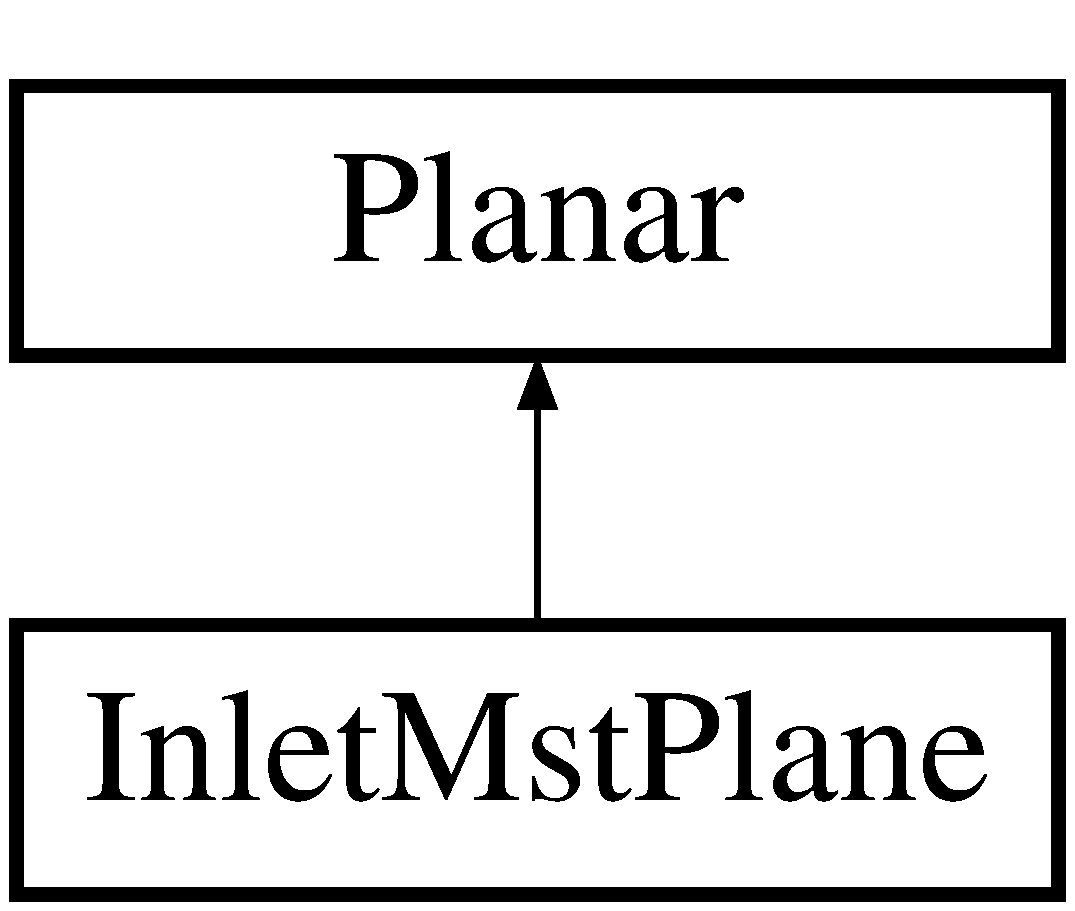
\includegraphics[height=2.000000cm]{d6/d96/class_inlet_mst_plane}
\end{center}
\end{figure}
\subsection*{Public Member Functions}
\begin{DoxyCompactItemize}
\item 
\mbox{\Hypertarget{class_inlet_mst_plane_a28e49257446ce8eaffe85e5208a37679}\label{class_inlet_mst_plane_a28e49257446ce8eaffe85e5208a37679}} 
{\bfseries Inlet\+Mst\+Plane} (double circular\+Duct\+Diameter, double tdx, double pbx, double psx)
\item 
\mbox{\Hypertarget{class_inlet_mst_plane_a7ef5ba8a7f1cbb55236ca97418d78a56}\label{class_inlet_mst_plane_a7ef5ba8a7f1cbb55236ca97418d78a56}} 
{\bfseries Inlet\+Mst\+Plane} (double rect\+Length, double rect\+Width, double tdx, double pbx, double psx)
\item 
\mbox{\Hypertarget{class_inlet_mst_plane_ab29a93aa3ac15b676590499bc91d387e}\label{class_inlet_mst_plane_ab29a93aa3ac15b676590499bc91d387e}} 
{\bfseries Inlet\+Mst\+Plane} (double rect\+Length, double rect\+Width, unsigned no\+Inlet\+Boxes, double tdx, double pbx, double psx)
\end{DoxyCompactItemize}
\subsection*{Additional Inherited Members}


\subsection{Detailed Description}


Definition at line 100 of file Planar.\+h.



The documentation for this class was generated from the following files\+:\begin{DoxyCompactItemize}
\item 
include/fans/Planar.\+h\item 
src/fans/Planar.\+cpp\end{DoxyCompactItemize}

\hypertarget{class_leakage_losses}{}\section{Leakage\+Losses Class Reference}
\label{class_leakage_losses}\index{Leakage\+Losses@{Leakage\+Losses}}


{\ttfamily \#include $<$Leakage\+Losses.\+h$>$}

\subsection*{Public Member Functions}
\begin{DoxyCompactItemize}
\item 
\hyperlink{class_leakage_losses_ab29a3d7c9561d73f2530fc376b528510}{Leakage\+Losses} (double draft\+Pressure, double opening\+Area, double leakage\+Gas\+Temperature, double ambient\+Temperature, double coefficient, double specific\+Gravity, double correction\+Factor)
\item 
double \hyperlink{class_leakage_losses_a0ec89fc6371c4a788e1bb861c7cfba35}{get\+Draft\+Pressure} () const
\item 
void \hyperlink{class_leakage_losses_a33f31dc336fc6af0fd1e8c8739f37b1a}{set\+Draft\+Pressure} (double draft\+Pressure)
\item 
double \hyperlink{class_leakage_losses_a6b31fbefaa16a5a52ce423b9531e84fa}{get\+Opening\+Area} () const
\item 
void \hyperlink{class_leakage_losses_a417c9914af6b283695bdbd5e92451f9e}{set\+Opening\+Area} (double opening\+Area)
\item 
double \hyperlink{class_leakage_losses_a5dbb249c07bc91611b71d62610af7234}{get\+Leakage\+Gas\+Temperature} () const
\item 
void \hyperlink{class_leakage_losses_a379c88c8dea822636a1b9966e2408daa}{set\+Leakage\+Gas\+Temperature} (double leakage\+Gas\+Temperature)
\item 
double \hyperlink{class_leakage_losses_af67ad0af750484b13dd311c881f71c61}{get\+Ambient\+Temperature} () const
\item 
void \hyperlink{class_leakage_losses_aa6028111b3eb305d9ea6f9efea7c6c66}{set\+Ambient\+Temperature} (double ambient\+Temperature)
\item 
double \hyperlink{class_leakage_losses_a7f70af7175574e0c4447a322586ac01e}{get\+Coefficient} () const
\item 
void \hyperlink{class_leakage_losses_add2e96e75b6dd965370340dc03717434}{set\+Coefficient} (double coefficient)
\item 
double \hyperlink{class_leakage_losses_a37cd8c2282547246bab395424dad51d9}{get\+Specific\+Gravity} () const
\item 
void \hyperlink{class_leakage_losses_ab017828413655c5903374564e8718fac}{set\+Specific\+Gravity} (double specific\+Gravity)
\item 
double \hyperlink{class_leakage_losses_ad4f289a7490cd3fd4dfc4099fc4ad562}{get\+Correction\+Factor} () const
\item 
void \hyperlink{class_leakage_losses_a1af53750d5d9573dffa8674b3479e8d6}{set\+Correction\+Factor} (double correction\+Factor)
\item 
double \hyperlink{class_leakage_losses_a9663b916752bcf39a5482674e225e4a5}{get\+Exfiltrated\+Gases\+Heat\+Content} ()
\item 
\hyperlink{class_leakage_losses_ab29a3d7c9561d73f2530fc376b528510}{Leakage\+Losses} (double draft\+Pressure, double opening\+Area, double leakage\+Gas\+Temperature, double ambient\+Temperature, double coefficient, double specific\+Gravity, double correction\+Factor)
\item 
double \hyperlink{class_leakage_losses_a0ec89fc6371c4a788e1bb861c7cfba35}{get\+Draft\+Pressure} () const
\item 
void \hyperlink{class_leakage_losses_a33f31dc336fc6af0fd1e8c8739f37b1a}{set\+Draft\+Pressure} (double draft\+Pressure)
\item 
double \hyperlink{class_leakage_losses_a6b31fbefaa16a5a52ce423b9531e84fa}{get\+Opening\+Area} () const
\item 
void \hyperlink{class_leakage_losses_a417c9914af6b283695bdbd5e92451f9e}{set\+Opening\+Area} (double opening\+Area)
\item 
double \hyperlink{class_leakage_losses_a5dbb249c07bc91611b71d62610af7234}{get\+Leakage\+Gas\+Temperature} () const
\item 
void \hyperlink{class_leakage_losses_a379c88c8dea822636a1b9966e2408daa}{set\+Leakage\+Gas\+Temperature} (double leakage\+Gas\+Temperature)
\item 
double \hyperlink{class_leakage_losses_af67ad0af750484b13dd311c881f71c61}{get\+Ambient\+Temperature} () const
\item 
void \hyperlink{class_leakage_losses_aa6028111b3eb305d9ea6f9efea7c6c66}{set\+Ambient\+Temperature} (double ambient\+Temperature)
\item 
double \hyperlink{class_leakage_losses_a7f70af7175574e0c4447a322586ac01e}{get\+Coefficient} () const
\item 
void \hyperlink{class_leakage_losses_add2e96e75b6dd965370340dc03717434}{set\+Coefficient} (double coefficient)
\item 
double \hyperlink{class_leakage_losses_a37cd8c2282547246bab395424dad51d9}{get\+Specific\+Gravity} () const
\item 
void \hyperlink{class_leakage_losses_ab017828413655c5903374564e8718fac}{set\+Specific\+Gravity} (double specific\+Gravity)
\item 
double \hyperlink{class_leakage_losses_ad4f289a7490cd3fd4dfc4099fc4ad562}{get\+Correction\+Factor} () const
\item 
void \hyperlink{class_leakage_losses_a1af53750d5d9573dffa8674b3479e8d6}{set\+Correction\+Factor} (double correction\+Factor)
\item 
double \hyperlink{class_leakage_losses_a9663b916752bcf39a5482674e225e4a5}{get\+Exfiltrated\+Gases\+Heat\+Content} ()
\item 
\hyperlink{class_leakage_losses_ab29a3d7c9561d73f2530fc376b528510}{Leakage\+Losses} (double draft\+Pressure, double opening\+Area, double leakage\+Gas\+Temperature, double ambient\+Temperature, double coefficient, double specific\+Gravity, double correction\+Factor)
\item 
double \hyperlink{class_leakage_losses_a0ec89fc6371c4a788e1bb861c7cfba35}{get\+Draft\+Pressure} () const
\item 
void \hyperlink{class_leakage_losses_a33f31dc336fc6af0fd1e8c8739f37b1a}{set\+Draft\+Pressure} (double draft\+Pressure)
\item 
double \hyperlink{class_leakage_losses_a6b31fbefaa16a5a52ce423b9531e84fa}{get\+Opening\+Area} () const
\item 
void \hyperlink{class_leakage_losses_a417c9914af6b283695bdbd5e92451f9e}{set\+Opening\+Area} (double opening\+Area)
\item 
double \hyperlink{class_leakage_losses_a5dbb249c07bc91611b71d62610af7234}{get\+Leakage\+Gas\+Temperature} () const
\item 
void \hyperlink{class_leakage_losses_a379c88c8dea822636a1b9966e2408daa}{set\+Leakage\+Gas\+Temperature} (double leakage\+Gas\+Temperature)
\item 
double \hyperlink{class_leakage_losses_af67ad0af750484b13dd311c881f71c61}{get\+Ambient\+Temperature} () const
\item 
void \hyperlink{class_leakage_losses_aa6028111b3eb305d9ea6f9efea7c6c66}{set\+Ambient\+Temperature} (double ambient\+Temperature)
\item 
double \hyperlink{class_leakage_losses_a7f70af7175574e0c4447a322586ac01e}{get\+Coefficient} () const
\item 
void \hyperlink{class_leakage_losses_add2e96e75b6dd965370340dc03717434}{set\+Coefficient} (double coefficient)
\item 
double \hyperlink{class_leakage_losses_a37cd8c2282547246bab395424dad51d9}{get\+Specific\+Gravity} () const
\item 
void \hyperlink{class_leakage_losses_ab017828413655c5903374564e8718fac}{set\+Specific\+Gravity} (double specific\+Gravity)
\item 
double \hyperlink{class_leakage_losses_ad4f289a7490cd3fd4dfc4099fc4ad562}{get\+Correction\+Factor} () const
\item 
void \hyperlink{class_leakage_losses_a1af53750d5d9573dffa8674b3479e8d6}{set\+Correction\+Factor} (double correction\+Factor)
\item 
double \hyperlink{class_leakage_losses_a9663b916752bcf39a5482674e225e4a5}{get\+Exfiltrated\+Gases\+Heat\+Content} ()
\end{DoxyCompactItemize}


\subsection{Detailed Description}
Leakage Losses class Contains all of the properties of a hot gas leakage. Used to calculate the heat loss caused by gases leaving the furnace via openings other then the flue. This calculator should only be used if the furnace is operating at a positive pressure. 

Definition at line 23 of file Leakage\+Losses.\+h.



\subsection{Constructor \& Destructor Documentation}
\mbox{\Hypertarget{class_leakage_losses_ab29a3d7c9561d73f2530fc376b528510}\label{class_leakage_losses_ab29a3d7c9561d73f2530fc376b528510}} 
\index{Leakage\+Losses@{Leakage\+Losses}!Leakage\+Losses@{Leakage\+Losses}}
\index{Leakage\+Losses@{Leakage\+Losses}!Leakage\+Losses@{Leakage\+Losses}}
\subsubsection{\texorpdfstring{Leakage\+Losses()}{LeakageLosses()}\hspace{0.1cm}{\footnotesize\ttfamily [1/3]}}
{\footnotesize\ttfamily Leakage\+Losses\+::\+Leakage\+Losses (\begin{DoxyParamCaption}\item[{double}]{draft\+Pressure,  }\item[{double}]{opening\+Area,  }\item[{double}]{leakage\+Gas\+Temperature,  }\item[{double}]{ambient\+Temperature,  }\item[{double}]{coefficient,  }\item[{double}]{specific\+Gravity,  }\item[{double}]{correction\+Factor }\end{DoxyParamCaption})\hspace{0.3cm}{\ttfamily [inline]}}

Constructor 
\begin{DoxyParams}{Parameters}
{\em draft\+Pressure} & double, furnace draft pressure in inch W.\+C. \\
\hline
{\em opening\+Area} & double, opening area in ft$^\wedge$2 \\
\hline
{\em leakage\+Gas\+Temperature} & double, temperature of gases leaking from furnace in °F \\
\hline
{\em ambient\+Temperature} & double. ambient temperature in °F \\
\hline
{\em coefficient} & double, coefficient -\/ unitless \\
\hline
{\em specific\+Gravity} & double, specific gravity -\/ unitless \\
\hline
{\em correction\+Factor} & double, correction factor -\/ unitless \\
\hline
\end{DoxyParams}


Definition at line 35 of file Leakage\+Losses.\+h.

\mbox{\Hypertarget{class_leakage_losses_ab29a3d7c9561d73f2530fc376b528510}\label{class_leakage_losses_ab29a3d7c9561d73f2530fc376b528510}} 
\index{Leakage\+Losses@{Leakage\+Losses}!Leakage\+Losses@{Leakage\+Losses}}
\index{Leakage\+Losses@{Leakage\+Losses}!Leakage\+Losses@{Leakage\+Losses}}
\subsubsection{\texorpdfstring{Leakage\+Losses()}{LeakageLosses()}\hspace{0.1cm}{\footnotesize\ttfamily [2/3]}}
{\footnotesize\ttfamily Leakage\+Losses\+::\+Leakage\+Losses (\begin{DoxyParamCaption}\item[{double}]{draft\+Pressure,  }\item[{double}]{opening\+Area,  }\item[{double}]{leakage\+Gas\+Temperature,  }\item[{double}]{ambient\+Temperature,  }\item[{double}]{coefficient,  }\item[{double}]{specific\+Gravity,  }\item[{double}]{correction\+Factor }\end{DoxyParamCaption})\hspace{0.3cm}{\ttfamily [inline]}}

Constructor 
\begin{DoxyParams}{Parameters}
{\em draft\+Pressure} & double, furnace draft pressure in inch W.\+C. \\
\hline
{\em opening\+Area} & double, opening area in ft$^\wedge$2 \\
\hline
{\em leakage\+Gas\+Temperature} & double, temperature of gases leaking from furnace in °F \\
\hline
{\em ambient\+Temperature} & double. ambient temperature in °F \\
\hline
{\em coefficient} & double, coefficient -\/ unitless \\
\hline
{\em specific\+Gravity} & double, specific gravity -\/ unitless \\
\hline
{\em correction\+Factor} & double, correction factor -\/ unitless \\
\hline
\end{DoxyParams}


Definition at line 35 of file Leakage\+Losses.\+h.

\mbox{\Hypertarget{class_leakage_losses_ab29a3d7c9561d73f2530fc376b528510}\label{class_leakage_losses_ab29a3d7c9561d73f2530fc376b528510}} 
\index{Leakage\+Losses@{Leakage\+Losses}!Leakage\+Losses@{Leakage\+Losses}}
\index{Leakage\+Losses@{Leakage\+Losses}!Leakage\+Losses@{Leakage\+Losses}}
\subsubsection{\texorpdfstring{Leakage\+Losses()}{LeakageLosses()}\hspace{0.1cm}{\footnotesize\ttfamily [3/3]}}
{\footnotesize\ttfamily Leakage\+Losses\+::\+Leakage\+Losses (\begin{DoxyParamCaption}\item[{double}]{draft\+Pressure,  }\item[{double}]{opening\+Area,  }\item[{double}]{leakage\+Gas\+Temperature,  }\item[{double}]{ambient\+Temperature,  }\item[{double}]{coefficient,  }\item[{double}]{specific\+Gravity,  }\item[{double}]{correction\+Factor }\end{DoxyParamCaption})\hspace{0.3cm}{\ttfamily [inline]}}

Constructor 
\begin{DoxyParams}{Parameters}
{\em draft\+Pressure} & double, furnace draft pressure in inch W.\+C. \\
\hline
{\em opening\+Area} & double, opening area in ft$^\wedge$2 \\
\hline
{\em leakage\+Gas\+Temperature} & double, temperature of gases leaking from furnace in °F \\
\hline
{\em ambient\+Temperature} & double. ambient temperature in °F \\
\hline
{\em coefficient} & double, coefficient -\/ unitless \\
\hline
{\em specific\+Gravity} & double, specific gravity -\/ unitless \\
\hline
{\em correction\+Factor} & double, correction factor -\/ unitless \\
\hline
\end{DoxyParams}


Definition at line 35 of file Leakage\+Losses.\+h.



\subsection{Member Function Documentation}
\mbox{\Hypertarget{class_leakage_losses_af67ad0af750484b13dd311c881f71c61}\label{class_leakage_losses_af67ad0af750484b13dd311c881f71c61}} 
\index{Leakage\+Losses@{Leakage\+Losses}!get\+Ambient\+Temperature@{get\+Ambient\+Temperature}}
\index{get\+Ambient\+Temperature@{get\+Ambient\+Temperature}!Leakage\+Losses@{Leakage\+Losses}}
\subsubsection{\texorpdfstring{get\+Ambient\+Temperature()}{getAmbientTemperature()}\hspace{0.1cm}{\footnotesize\ttfamily [1/3]}}
{\footnotesize\ttfamily double Leakage\+Losses\+::get\+Ambient\+Temperature (\begin{DoxyParamCaption}{ }\end{DoxyParamCaption}) const\hspace{0.3cm}{\ttfamily [inline]}}

Gets the ambient temperature \begin{DoxyReturn}{Returns}
double, ambient temperature in °F 
\end{DoxyReturn}


Definition at line 108 of file Leakage\+Losses.\+h.

\mbox{\Hypertarget{class_leakage_losses_af67ad0af750484b13dd311c881f71c61}\label{class_leakage_losses_af67ad0af750484b13dd311c881f71c61}} 
\index{Leakage\+Losses@{Leakage\+Losses}!get\+Ambient\+Temperature@{get\+Ambient\+Temperature}}
\index{get\+Ambient\+Temperature@{get\+Ambient\+Temperature}!Leakage\+Losses@{Leakage\+Losses}}
\subsubsection{\texorpdfstring{get\+Ambient\+Temperature()}{getAmbientTemperature()}\hspace{0.1cm}{\footnotesize\ttfamily [2/3]}}
{\footnotesize\ttfamily double Leakage\+Losses\+::get\+Ambient\+Temperature (\begin{DoxyParamCaption}{ }\end{DoxyParamCaption}) const\hspace{0.3cm}{\ttfamily [inline]}}

Gets the ambient temperature \begin{DoxyReturn}{Returns}
double, ambient temperature in °F 
\end{DoxyReturn}


Definition at line 108 of file Leakage\+Losses.\+h.

\mbox{\Hypertarget{class_leakage_losses_af67ad0af750484b13dd311c881f71c61}\label{class_leakage_losses_af67ad0af750484b13dd311c881f71c61}} 
\index{Leakage\+Losses@{Leakage\+Losses}!get\+Ambient\+Temperature@{get\+Ambient\+Temperature}}
\index{get\+Ambient\+Temperature@{get\+Ambient\+Temperature}!Leakage\+Losses@{Leakage\+Losses}}
\subsubsection{\texorpdfstring{get\+Ambient\+Temperature()}{getAmbientTemperature()}\hspace{0.1cm}{\footnotesize\ttfamily [3/3]}}
{\footnotesize\ttfamily double Leakage\+Losses\+::get\+Ambient\+Temperature (\begin{DoxyParamCaption}{ }\end{DoxyParamCaption}) const\hspace{0.3cm}{\ttfamily [inline]}}

Gets the ambient temperature \begin{DoxyReturn}{Returns}
double, ambient temperature in °F 
\end{DoxyReturn}


Definition at line 108 of file Leakage\+Losses.\+h.

\mbox{\Hypertarget{class_leakage_losses_a7f70af7175574e0c4447a322586ac01e}\label{class_leakage_losses_a7f70af7175574e0c4447a322586ac01e}} 
\index{Leakage\+Losses@{Leakage\+Losses}!get\+Coefficient@{get\+Coefficient}}
\index{get\+Coefficient@{get\+Coefficient}!Leakage\+Losses@{Leakage\+Losses}}
\subsubsection{\texorpdfstring{get\+Coefficient()}{getCoefficient()}\hspace{0.1cm}{\footnotesize\ttfamily [1/3]}}
{\footnotesize\ttfamily double Leakage\+Losses\+::get\+Coefficient (\begin{DoxyParamCaption}{ }\end{DoxyParamCaption}) const\hspace{0.3cm}{\ttfamily [inline]}}

Gets the coefficient \begin{DoxyReturn}{Returns}
double, coefficient -\/ unitless 
\end{DoxyReturn}


Definition at line 124 of file Leakage\+Losses.\+h.

\mbox{\Hypertarget{class_leakage_losses_a7f70af7175574e0c4447a322586ac01e}\label{class_leakage_losses_a7f70af7175574e0c4447a322586ac01e}} 
\index{Leakage\+Losses@{Leakage\+Losses}!get\+Coefficient@{get\+Coefficient}}
\index{get\+Coefficient@{get\+Coefficient}!Leakage\+Losses@{Leakage\+Losses}}
\subsubsection{\texorpdfstring{get\+Coefficient()}{getCoefficient()}\hspace{0.1cm}{\footnotesize\ttfamily [2/3]}}
{\footnotesize\ttfamily double Leakage\+Losses\+::get\+Coefficient (\begin{DoxyParamCaption}{ }\end{DoxyParamCaption}) const\hspace{0.3cm}{\ttfamily [inline]}}

Gets the coefficient \begin{DoxyReturn}{Returns}
double, coefficient -\/ unitless 
\end{DoxyReturn}


Definition at line 124 of file Leakage\+Losses.\+h.

\mbox{\Hypertarget{class_leakage_losses_a7f70af7175574e0c4447a322586ac01e}\label{class_leakage_losses_a7f70af7175574e0c4447a322586ac01e}} 
\index{Leakage\+Losses@{Leakage\+Losses}!get\+Coefficient@{get\+Coefficient}}
\index{get\+Coefficient@{get\+Coefficient}!Leakage\+Losses@{Leakage\+Losses}}
\subsubsection{\texorpdfstring{get\+Coefficient()}{getCoefficient()}\hspace{0.1cm}{\footnotesize\ttfamily [3/3]}}
{\footnotesize\ttfamily double Leakage\+Losses\+::get\+Coefficient (\begin{DoxyParamCaption}{ }\end{DoxyParamCaption}) const\hspace{0.3cm}{\ttfamily [inline]}}

Gets the coefficient \begin{DoxyReturn}{Returns}
double, coefficient -\/ unitless 
\end{DoxyReturn}


Definition at line 124 of file Leakage\+Losses.\+h.

\mbox{\Hypertarget{class_leakage_losses_ad4f289a7490cd3fd4dfc4099fc4ad562}\label{class_leakage_losses_ad4f289a7490cd3fd4dfc4099fc4ad562}} 
\index{Leakage\+Losses@{Leakage\+Losses}!get\+Correction\+Factor@{get\+Correction\+Factor}}
\index{get\+Correction\+Factor@{get\+Correction\+Factor}!Leakage\+Losses@{Leakage\+Losses}}
\subsubsection{\texorpdfstring{get\+Correction\+Factor()}{getCorrectionFactor()}\hspace{0.1cm}{\footnotesize\ttfamily [1/3]}}
{\footnotesize\ttfamily double Leakage\+Losses\+::get\+Correction\+Factor (\begin{DoxyParamCaption}{ }\end{DoxyParamCaption}) const\hspace{0.3cm}{\ttfamily [inline]}}

Gets the correction factor \begin{DoxyReturn}{Returns}
double, correction factor -\/ unitless 
\end{DoxyReturn}


Definition at line 156 of file Leakage\+Losses.\+h.

\mbox{\Hypertarget{class_leakage_losses_ad4f289a7490cd3fd4dfc4099fc4ad562}\label{class_leakage_losses_ad4f289a7490cd3fd4dfc4099fc4ad562}} 
\index{Leakage\+Losses@{Leakage\+Losses}!get\+Correction\+Factor@{get\+Correction\+Factor}}
\index{get\+Correction\+Factor@{get\+Correction\+Factor}!Leakage\+Losses@{Leakage\+Losses}}
\subsubsection{\texorpdfstring{get\+Correction\+Factor()}{getCorrectionFactor()}\hspace{0.1cm}{\footnotesize\ttfamily [2/3]}}
{\footnotesize\ttfamily double Leakage\+Losses\+::get\+Correction\+Factor (\begin{DoxyParamCaption}{ }\end{DoxyParamCaption}) const\hspace{0.3cm}{\ttfamily [inline]}}

Gets the correction factor \begin{DoxyReturn}{Returns}
double, correction factor -\/ unitless 
\end{DoxyReturn}


Definition at line 156 of file Leakage\+Losses.\+h.

\mbox{\Hypertarget{class_leakage_losses_ad4f289a7490cd3fd4dfc4099fc4ad562}\label{class_leakage_losses_ad4f289a7490cd3fd4dfc4099fc4ad562}} 
\index{Leakage\+Losses@{Leakage\+Losses}!get\+Correction\+Factor@{get\+Correction\+Factor}}
\index{get\+Correction\+Factor@{get\+Correction\+Factor}!Leakage\+Losses@{Leakage\+Losses}}
\subsubsection{\texorpdfstring{get\+Correction\+Factor()}{getCorrectionFactor()}\hspace{0.1cm}{\footnotesize\ttfamily [3/3]}}
{\footnotesize\ttfamily double Leakage\+Losses\+::get\+Correction\+Factor (\begin{DoxyParamCaption}{ }\end{DoxyParamCaption}) const\hspace{0.3cm}{\ttfamily [inline]}}

Gets the correction factor \begin{DoxyReturn}{Returns}
double, correction factor -\/ unitless 
\end{DoxyReturn}


Definition at line 156 of file Leakage\+Losses.\+h.

\mbox{\Hypertarget{class_leakage_losses_a0ec89fc6371c4a788e1bb861c7cfba35}\label{class_leakage_losses_a0ec89fc6371c4a788e1bb861c7cfba35}} 
\index{Leakage\+Losses@{Leakage\+Losses}!get\+Draft\+Pressure@{get\+Draft\+Pressure}}
\index{get\+Draft\+Pressure@{get\+Draft\+Pressure}!Leakage\+Losses@{Leakage\+Losses}}
\subsubsection{\texorpdfstring{get\+Draft\+Pressure()}{getDraftPressure()}\hspace{0.1cm}{\footnotesize\ttfamily [1/3]}}
{\footnotesize\ttfamily double Leakage\+Losses\+::get\+Draft\+Pressure (\begin{DoxyParamCaption}{ }\end{DoxyParamCaption}) const\hspace{0.3cm}{\ttfamily [inline]}}

Gets the furnace draft pressure \begin{DoxyReturn}{Returns}
double, draft pressure in inch W.\+C. 
\end{DoxyReturn}


Definition at line 60 of file Leakage\+Losses.\+h.

\mbox{\Hypertarget{class_leakage_losses_a0ec89fc6371c4a788e1bb861c7cfba35}\label{class_leakage_losses_a0ec89fc6371c4a788e1bb861c7cfba35}} 
\index{Leakage\+Losses@{Leakage\+Losses}!get\+Draft\+Pressure@{get\+Draft\+Pressure}}
\index{get\+Draft\+Pressure@{get\+Draft\+Pressure}!Leakage\+Losses@{Leakage\+Losses}}
\subsubsection{\texorpdfstring{get\+Draft\+Pressure()}{getDraftPressure()}\hspace{0.1cm}{\footnotesize\ttfamily [2/3]}}
{\footnotesize\ttfamily double Leakage\+Losses\+::get\+Draft\+Pressure (\begin{DoxyParamCaption}{ }\end{DoxyParamCaption}) const\hspace{0.3cm}{\ttfamily [inline]}}

Gets the furnace draft pressure \begin{DoxyReturn}{Returns}
double, draft pressure in inch W.\+C. 
\end{DoxyReturn}


Definition at line 60 of file Leakage\+Losses.\+h.

\mbox{\Hypertarget{class_leakage_losses_a0ec89fc6371c4a788e1bb861c7cfba35}\label{class_leakage_losses_a0ec89fc6371c4a788e1bb861c7cfba35}} 
\index{Leakage\+Losses@{Leakage\+Losses}!get\+Draft\+Pressure@{get\+Draft\+Pressure}}
\index{get\+Draft\+Pressure@{get\+Draft\+Pressure}!Leakage\+Losses@{Leakage\+Losses}}
\subsubsection{\texorpdfstring{get\+Draft\+Pressure()}{getDraftPressure()}\hspace{0.1cm}{\footnotesize\ttfamily [3/3]}}
{\footnotesize\ttfamily double Leakage\+Losses\+::get\+Draft\+Pressure (\begin{DoxyParamCaption}{ }\end{DoxyParamCaption}) const\hspace{0.3cm}{\ttfamily [inline]}}

Gets the furnace draft pressure \begin{DoxyReturn}{Returns}
double, draft pressure in inch W.\+C. 
\end{DoxyReturn}


Definition at line 60 of file Leakage\+Losses.\+h.

\mbox{\Hypertarget{class_leakage_losses_a9663b916752bcf39a5482674e225e4a5}\label{class_leakage_losses_a9663b916752bcf39a5482674e225e4a5}} 
\index{Leakage\+Losses@{Leakage\+Losses}!get\+Exfiltrated\+Gases\+Heat\+Content@{get\+Exfiltrated\+Gases\+Heat\+Content}}
\index{get\+Exfiltrated\+Gases\+Heat\+Content@{get\+Exfiltrated\+Gases\+Heat\+Content}!Leakage\+Losses@{Leakage\+Losses}}
\subsubsection{\texorpdfstring{get\+Exfiltrated\+Gases\+Heat\+Content()}{getExfiltratedGasesHeatContent()}\hspace{0.1cm}{\footnotesize\ttfamily [1/3]}}
{\footnotesize\ttfamily double Leakage\+Losses\+::get\+Exfiltrated\+Gases\+Heat\+Content (\begin{DoxyParamCaption}{ }\end{DoxyParamCaption})}

Gets the exfiltrated gases heat content \begin{DoxyReturn}{Returns}
double, exfiltrated gases heat content in btu/hr 
\end{DoxyReturn}
\mbox{\Hypertarget{class_leakage_losses_a9663b916752bcf39a5482674e225e4a5}\label{class_leakage_losses_a9663b916752bcf39a5482674e225e4a5}} 
\index{Leakage\+Losses@{Leakage\+Losses}!get\+Exfiltrated\+Gases\+Heat\+Content@{get\+Exfiltrated\+Gases\+Heat\+Content}}
\index{get\+Exfiltrated\+Gases\+Heat\+Content@{get\+Exfiltrated\+Gases\+Heat\+Content}!Leakage\+Losses@{Leakage\+Losses}}
\subsubsection{\texorpdfstring{get\+Exfiltrated\+Gases\+Heat\+Content()}{getExfiltratedGasesHeatContent()}\hspace{0.1cm}{\footnotesize\ttfamily [2/3]}}
{\footnotesize\ttfamily double Leakage\+Losses\+::get\+Exfiltrated\+Gases\+Heat\+Content (\begin{DoxyParamCaption}{ }\end{DoxyParamCaption})}

Gets the exfiltrated gases heat content \begin{DoxyReturn}{Returns}
double, exfiltrated gases heat content in btu/hr 
\end{DoxyReturn}


Definition at line 13 of file Leakage\+Losses.\+cpp.

\mbox{\Hypertarget{class_leakage_losses_a9663b916752bcf39a5482674e225e4a5}\label{class_leakage_losses_a9663b916752bcf39a5482674e225e4a5}} 
\index{Leakage\+Losses@{Leakage\+Losses}!get\+Exfiltrated\+Gases\+Heat\+Content@{get\+Exfiltrated\+Gases\+Heat\+Content}}
\index{get\+Exfiltrated\+Gases\+Heat\+Content@{get\+Exfiltrated\+Gases\+Heat\+Content}!Leakage\+Losses@{Leakage\+Losses}}
\subsubsection{\texorpdfstring{get\+Exfiltrated\+Gases\+Heat\+Content()}{getExfiltratedGasesHeatContent()}\hspace{0.1cm}{\footnotesize\ttfamily [3/3]}}
{\footnotesize\ttfamily double Leakage\+Losses\+::get\+Exfiltrated\+Gases\+Heat\+Content (\begin{DoxyParamCaption}{ }\end{DoxyParamCaption})}

Gets the exfiltrated gases heat content \begin{DoxyReturn}{Returns}
double, exfiltrated gases heat content in btu/hr 
\end{DoxyReturn}
\mbox{\Hypertarget{class_leakage_losses_a5dbb249c07bc91611b71d62610af7234}\label{class_leakage_losses_a5dbb249c07bc91611b71d62610af7234}} 
\index{Leakage\+Losses@{Leakage\+Losses}!get\+Leakage\+Gas\+Temperature@{get\+Leakage\+Gas\+Temperature}}
\index{get\+Leakage\+Gas\+Temperature@{get\+Leakage\+Gas\+Temperature}!Leakage\+Losses@{Leakage\+Losses}}
\subsubsection{\texorpdfstring{get\+Leakage\+Gas\+Temperature()}{getLeakageGasTemperature()}\hspace{0.1cm}{\footnotesize\ttfamily [1/3]}}
{\footnotesize\ttfamily double Leakage\+Losses\+::get\+Leakage\+Gas\+Temperature (\begin{DoxyParamCaption}{ }\end{DoxyParamCaption}) const\hspace{0.3cm}{\ttfamily [inline]}}

Gets the temperature of gases leaking from furnace \begin{DoxyReturn}{Returns}
double, leakeage gas temperature in °F 
\end{DoxyReturn}


Definition at line 92 of file Leakage\+Losses.\+h.

\mbox{\Hypertarget{class_leakage_losses_a5dbb249c07bc91611b71d62610af7234}\label{class_leakage_losses_a5dbb249c07bc91611b71d62610af7234}} 
\index{Leakage\+Losses@{Leakage\+Losses}!get\+Leakage\+Gas\+Temperature@{get\+Leakage\+Gas\+Temperature}}
\index{get\+Leakage\+Gas\+Temperature@{get\+Leakage\+Gas\+Temperature}!Leakage\+Losses@{Leakage\+Losses}}
\subsubsection{\texorpdfstring{get\+Leakage\+Gas\+Temperature()}{getLeakageGasTemperature()}\hspace{0.1cm}{\footnotesize\ttfamily [2/3]}}
{\footnotesize\ttfamily double Leakage\+Losses\+::get\+Leakage\+Gas\+Temperature (\begin{DoxyParamCaption}{ }\end{DoxyParamCaption}) const\hspace{0.3cm}{\ttfamily [inline]}}

Gets the temperature of gases leaking from furnace \begin{DoxyReturn}{Returns}
double, leakeage gas temperature in °F 
\end{DoxyReturn}


Definition at line 92 of file Leakage\+Losses.\+h.

\mbox{\Hypertarget{class_leakage_losses_a5dbb249c07bc91611b71d62610af7234}\label{class_leakage_losses_a5dbb249c07bc91611b71d62610af7234}} 
\index{Leakage\+Losses@{Leakage\+Losses}!get\+Leakage\+Gas\+Temperature@{get\+Leakage\+Gas\+Temperature}}
\index{get\+Leakage\+Gas\+Temperature@{get\+Leakage\+Gas\+Temperature}!Leakage\+Losses@{Leakage\+Losses}}
\subsubsection{\texorpdfstring{get\+Leakage\+Gas\+Temperature()}{getLeakageGasTemperature()}\hspace{0.1cm}{\footnotesize\ttfamily [3/3]}}
{\footnotesize\ttfamily double Leakage\+Losses\+::get\+Leakage\+Gas\+Temperature (\begin{DoxyParamCaption}{ }\end{DoxyParamCaption}) const\hspace{0.3cm}{\ttfamily [inline]}}

Gets the temperature of gases leaking from furnace \begin{DoxyReturn}{Returns}
double, leakeage gas temperature in °F 
\end{DoxyReturn}


Definition at line 92 of file Leakage\+Losses.\+h.

\mbox{\Hypertarget{class_leakage_losses_a6b31fbefaa16a5a52ce423b9531e84fa}\label{class_leakage_losses_a6b31fbefaa16a5a52ce423b9531e84fa}} 
\index{Leakage\+Losses@{Leakage\+Losses}!get\+Opening\+Area@{get\+Opening\+Area}}
\index{get\+Opening\+Area@{get\+Opening\+Area}!Leakage\+Losses@{Leakage\+Losses}}
\subsubsection{\texorpdfstring{get\+Opening\+Area()}{getOpeningArea()}\hspace{0.1cm}{\footnotesize\ttfamily [1/3]}}
{\footnotesize\ttfamily double Leakage\+Losses\+::get\+Opening\+Area (\begin{DoxyParamCaption}{ }\end{DoxyParamCaption}) const\hspace{0.3cm}{\ttfamily [inline]}}

Gets the opening area \begin{DoxyReturn}{Returns}
double, opening area in ft$^\wedge$2 
\end{DoxyReturn}


Definition at line 76 of file Leakage\+Losses.\+h.

\mbox{\Hypertarget{class_leakage_losses_a6b31fbefaa16a5a52ce423b9531e84fa}\label{class_leakage_losses_a6b31fbefaa16a5a52ce423b9531e84fa}} 
\index{Leakage\+Losses@{Leakage\+Losses}!get\+Opening\+Area@{get\+Opening\+Area}}
\index{get\+Opening\+Area@{get\+Opening\+Area}!Leakage\+Losses@{Leakage\+Losses}}
\subsubsection{\texorpdfstring{get\+Opening\+Area()}{getOpeningArea()}\hspace{0.1cm}{\footnotesize\ttfamily [2/3]}}
{\footnotesize\ttfamily double Leakage\+Losses\+::get\+Opening\+Area (\begin{DoxyParamCaption}{ }\end{DoxyParamCaption}) const\hspace{0.3cm}{\ttfamily [inline]}}

Gets the opening area \begin{DoxyReturn}{Returns}
double, opening area in ft$^\wedge$2 
\end{DoxyReturn}


Definition at line 76 of file Leakage\+Losses.\+h.

\mbox{\Hypertarget{class_leakage_losses_a6b31fbefaa16a5a52ce423b9531e84fa}\label{class_leakage_losses_a6b31fbefaa16a5a52ce423b9531e84fa}} 
\index{Leakage\+Losses@{Leakage\+Losses}!get\+Opening\+Area@{get\+Opening\+Area}}
\index{get\+Opening\+Area@{get\+Opening\+Area}!Leakage\+Losses@{Leakage\+Losses}}
\subsubsection{\texorpdfstring{get\+Opening\+Area()}{getOpeningArea()}\hspace{0.1cm}{\footnotesize\ttfamily [3/3]}}
{\footnotesize\ttfamily double Leakage\+Losses\+::get\+Opening\+Area (\begin{DoxyParamCaption}{ }\end{DoxyParamCaption}) const\hspace{0.3cm}{\ttfamily [inline]}}

Gets the opening area \begin{DoxyReturn}{Returns}
double, opening area in ft$^\wedge$2 
\end{DoxyReturn}


Definition at line 76 of file Leakage\+Losses.\+h.

\mbox{\Hypertarget{class_leakage_losses_a37cd8c2282547246bab395424dad51d9}\label{class_leakage_losses_a37cd8c2282547246bab395424dad51d9}} 
\index{Leakage\+Losses@{Leakage\+Losses}!get\+Specific\+Gravity@{get\+Specific\+Gravity}}
\index{get\+Specific\+Gravity@{get\+Specific\+Gravity}!Leakage\+Losses@{Leakage\+Losses}}
\subsubsection{\texorpdfstring{get\+Specific\+Gravity()}{getSpecificGravity()}\hspace{0.1cm}{\footnotesize\ttfamily [1/3]}}
{\footnotesize\ttfamily double Leakage\+Losses\+::get\+Specific\+Gravity (\begin{DoxyParamCaption}{ }\end{DoxyParamCaption}) const\hspace{0.3cm}{\ttfamily [inline]}}

Gets the specific gravity \begin{DoxyReturn}{Returns}
double, specific gravity -\/ unitless 
\end{DoxyReturn}


Definition at line 140 of file Leakage\+Losses.\+h.

\mbox{\Hypertarget{class_leakage_losses_a37cd8c2282547246bab395424dad51d9}\label{class_leakage_losses_a37cd8c2282547246bab395424dad51d9}} 
\index{Leakage\+Losses@{Leakage\+Losses}!get\+Specific\+Gravity@{get\+Specific\+Gravity}}
\index{get\+Specific\+Gravity@{get\+Specific\+Gravity}!Leakage\+Losses@{Leakage\+Losses}}
\subsubsection{\texorpdfstring{get\+Specific\+Gravity()}{getSpecificGravity()}\hspace{0.1cm}{\footnotesize\ttfamily [2/3]}}
{\footnotesize\ttfamily double Leakage\+Losses\+::get\+Specific\+Gravity (\begin{DoxyParamCaption}{ }\end{DoxyParamCaption}) const\hspace{0.3cm}{\ttfamily [inline]}}

Gets the specific gravity \begin{DoxyReturn}{Returns}
double, specific gravity -\/ unitless 
\end{DoxyReturn}


Definition at line 140 of file Leakage\+Losses.\+h.

\mbox{\Hypertarget{class_leakage_losses_a37cd8c2282547246bab395424dad51d9}\label{class_leakage_losses_a37cd8c2282547246bab395424dad51d9}} 
\index{Leakage\+Losses@{Leakage\+Losses}!get\+Specific\+Gravity@{get\+Specific\+Gravity}}
\index{get\+Specific\+Gravity@{get\+Specific\+Gravity}!Leakage\+Losses@{Leakage\+Losses}}
\subsubsection{\texorpdfstring{get\+Specific\+Gravity()}{getSpecificGravity()}\hspace{0.1cm}{\footnotesize\ttfamily [3/3]}}
{\footnotesize\ttfamily double Leakage\+Losses\+::get\+Specific\+Gravity (\begin{DoxyParamCaption}{ }\end{DoxyParamCaption}) const\hspace{0.3cm}{\ttfamily [inline]}}

Gets the specific gravity \begin{DoxyReturn}{Returns}
double, specific gravity -\/ unitless 
\end{DoxyReturn}


Definition at line 140 of file Leakage\+Losses.\+h.

\mbox{\Hypertarget{class_leakage_losses_aa6028111b3eb305d9ea6f9efea7c6c66}\label{class_leakage_losses_aa6028111b3eb305d9ea6f9efea7c6c66}} 
\index{Leakage\+Losses@{Leakage\+Losses}!set\+Ambient\+Temperature@{set\+Ambient\+Temperature}}
\index{set\+Ambient\+Temperature@{set\+Ambient\+Temperature}!Leakage\+Losses@{Leakage\+Losses}}
\subsubsection{\texorpdfstring{set\+Ambient\+Temperature()}{setAmbientTemperature()}\hspace{0.1cm}{\footnotesize\ttfamily [1/3]}}
{\footnotesize\ttfamily void Leakage\+Losses\+::set\+Ambient\+Temperature (\begin{DoxyParamCaption}\item[{double}]{ambient\+Temperature }\end{DoxyParamCaption})\hspace{0.3cm}{\ttfamily [inline]}}

Sets the ambient temperature 
\begin{DoxyParams}{Parameters}
{\em ambient\+Temperature} & double, ambient temperature in °F \\
\hline
\end{DoxyParams}


Definition at line 116 of file Leakage\+Losses.\+h.

\mbox{\Hypertarget{class_leakage_losses_aa6028111b3eb305d9ea6f9efea7c6c66}\label{class_leakage_losses_aa6028111b3eb305d9ea6f9efea7c6c66}} 
\index{Leakage\+Losses@{Leakage\+Losses}!set\+Ambient\+Temperature@{set\+Ambient\+Temperature}}
\index{set\+Ambient\+Temperature@{set\+Ambient\+Temperature}!Leakage\+Losses@{Leakage\+Losses}}
\subsubsection{\texorpdfstring{set\+Ambient\+Temperature()}{setAmbientTemperature()}\hspace{0.1cm}{\footnotesize\ttfamily [2/3]}}
{\footnotesize\ttfamily void Leakage\+Losses\+::set\+Ambient\+Temperature (\begin{DoxyParamCaption}\item[{double}]{ambient\+Temperature }\end{DoxyParamCaption})\hspace{0.3cm}{\ttfamily [inline]}}

Sets the ambient temperature 
\begin{DoxyParams}{Parameters}
{\em ambient\+Temperature} & double, ambient temperature in °F \\
\hline
\end{DoxyParams}


Definition at line 116 of file Leakage\+Losses.\+h.

\mbox{\Hypertarget{class_leakage_losses_aa6028111b3eb305d9ea6f9efea7c6c66}\label{class_leakage_losses_aa6028111b3eb305d9ea6f9efea7c6c66}} 
\index{Leakage\+Losses@{Leakage\+Losses}!set\+Ambient\+Temperature@{set\+Ambient\+Temperature}}
\index{set\+Ambient\+Temperature@{set\+Ambient\+Temperature}!Leakage\+Losses@{Leakage\+Losses}}
\subsubsection{\texorpdfstring{set\+Ambient\+Temperature()}{setAmbientTemperature()}\hspace{0.1cm}{\footnotesize\ttfamily [3/3]}}
{\footnotesize\ttfamily void Leakage\+Losses\+::set\+Ambient\+Temperature (\begin{DoxyParamCaption}\item[{double}]{ambient\+Temperature }\end{DoxyParamCaption})\hspace{0.3cm}{\ttfamily [inline]}}

Sets the ambient temperature 
\begin{DoxyParams}{Parameters}
{\em ambient\+Temperature} & double, ambient temperature in °F \\
\hline
\end{DoxyParams}


Definition at line 116 of file Leakage\+Losses.\+h.

\mbox{\Hypertarget{class_leakage_losses_add2e96e75b6dd965370340dc03717434}\label{class_leakage_losses_add2e96e75b6dd965370340dc03717434}} 
\index{Leakage\+Losses@{Leakage\+Losses}!set\+Coefficient@{set\+Coefficient}}
\index{set\+Coefficient@{set\+Coefficient}!Leakage\+Losses@{Leakage\+Losses}}
\subsubsection{\texorpdfstring{set\+Coefficient()}{setCoefficient()}\hspace{0.1cm}{\footnotesize\ttfamily [1/3]}}
{\footnotesize\ttfamily void Leakage\+Losses\+::set\+Coefficient (\begin{DoxyParamCaption}\item[{double}]{coefficient }\end{DoxyParamCaption})\hspace{0.3cm}{\ttfamily [inline]}}

Sets the coefficient 
\begin{DoxyParams}{Parameters}
{\em coefficient} & double, coefficient -\/ unitless \\
\hline
\end{DoxyParams}


Definition at line 132 of file Leakage\+Losses.\+h.

\mbox{\Hypertarget{class_leakage_losses_add2e96e75b6dd965370340dc03717434}\label{class_leakage_losses_add2e96e75b6dd965370340dc03717434}} 
\index{Leakage\+Losses@{Leakage\+Losses}!set\+Coefficient@{set\+Coefficient}}
\index{set\+Coefficient@{set\+Coefficient}!Leakage\+Losses@{Leakage\+Losses}}
\subsubsection{\texorpdfstring{set\+Coefficient()}{setCoefficient()}\hspace{0.1cm}{\footnotesize\ttfamily [2/3]}}
{\footnotesize\ttfamily void Leakage\+Losses\+::set\+Coefficient (\begin{DoxyParamCaption}\item[{double}]{coefficient }\end{DoxyParamCaption})\hspace{0.3cm}{\ttfamily [inline]}}

Sets the coefficient 
\begin{DoxyParams}{Parameters}
{\em coefficient} & double, coefficient -\/ unitless \\
\hline
\end{DoxyParams}


Definition at line 132 of file Leakage\+Losses.\+h.

\mbox{\Hypertarget{class_leakage_losses_add2e96e75b6dd965370340dc03717434}\label{class_leakage_losses_add2e96e75b6dd965370340dc03717434}} 
\index{Leakage\+Losses@{Leakage\+Losses}!set\+Coefficient@{set\+Coefficient}}
\index{set\+Coefficient@{set\+Coefficient}!Leakage\+Losses@{Leakage\+Losses}}
\subsubsection{\texorpdfstring{set\+Coefficient()}{setCoefficient()}\hspace{0.1cm}{\footnotesize\ttfamily [3/3]}}
{\footnotesize\ttfamily void Leakage\+Losses\+::set\+Coefficient (\begin{DoxyParamCaption}\item[{double}]{coefficient }\end{DoxyParamCaption})\hspace{0.3cm}{\ttfamily [inline]}}

Sets the coefficient 
\begin{DoxyParams}{Parameters}
{\em coefficient} & double, coefficient -\/ unitless \\
\hline
\end{DoxyParams}


Definition at line 132 of file Leakage\+Losses.\+h.

\mbox{\Hypertarget{class_leakage_losses_a1af53750d5d9573dffa8674b3479e8d6}\label{class_leakage_losses_a1af53750d5d9573dffa8674b3479e8d6}} 
\index{Leakage\+Losses@{Leakage\+Losses}!set\+Correction\+Factor@{set\+Correction\+Factor}}
\index{set\+Correction\+Factor@{set\+Correction\+Factor}!Leakage\+Losses@{Leakage\+Losses}}
\subsubsection{\texorpdfstring{set\+Correction\+Factor()}{setCorrectionFactor()}\hspace{0.1cm}{\footnotesize\ttfamily [1/3]}}
{\footnotesize\ttfamily void Leakage\+Losses\+::set\+Correction\+Factor (\begin{DoxyParamCaption}\item[{double}]{correction\+Factor }\end{DoxyParamCaption})\hspace{0.3cm}{\ttfamily [inline]}}

Sets the correction factor 
\begin{DoxyParams}{Parameters}
{\em correction\+Factor} & double, correction factor -\/ unitless \\
\hline
\end{DoxyParams}


Definition at line 164 of file Leakage\+Losses.\+h.

\mbox{\Hypertarget{class_leakage_losses_a1af53750d5d9573dffa8674b3479e8d6}\label{class_leakage_losses_a1af53750d5d9573dffa8674b3479e8d6}} 
\index{Leakage\+Losses@{Leakage\+Losses}!set\+Correction\+Factor@{set\+Correction\+Factor}}
\index{set\+Correction\+Factor@{set\+Correction\+Factor}!Leakage\+Losses@{Leakage\+Losses}}
\subsubsection{\texorpdfstring{set\+Correction\+Factor()}{setCorrectionFactor()}\hspace{0.1cm}{\footnotesize\ttfamily [2/3]}}
{\footnotesize\ttfamily void Leakage\+Losses\+::set\+Correction\+Factor (\begin{DoxyParamCaption}\item[{double}]{correction\+Factor }\end{DoxyParamCaption})\hspace{0.3cm}{\ttfamily [inline]}}

Sets the correction factor 
\begin{DoxyParams}{Parameters}
{\em correction\+Factor} & double, correction factor -\/ unitless \\
\hline
\end{DoxyParams}


Definition at line 164 of file Leakage\+Losses.\+h.

\mbox{\Hypertarget{class_leakage_losses_a1af53750d5d9573dffa8674b3479e8d6}\label{class_leakage_losses_a1af53750d5d9573dffa8674b3479e8d6}} 
\index{Leakage\+Losses@{Leakage\+Losses}!set\+Correction\+Factor@{set\+Correction\+Factor}}
\index{set\+Correction\+Factor@{set\+Correction\+Factor}!Leakage\+Losses@{Leakage\+Losses}}
\subsubsection{\texorpdfstring{set\+Correction\+Factor()}{setCorrectionFactor()}\hspace{0.1cm}{\footnotesize\ttfamily [3/3]}}
{\footnotesize\ttfamily void Leakage\+Losses\+::set\+Correction\+Factor (\begin{DoxyParamCaption}\item[{double}]{correction\+Factor }\end{DoxyParamCaption})\hspace{0.3cm}{\ttfamily [inline]}}

Sets the correction factor 
\begin{DoxyParams}{Parameters}
{\em correction\+Factor} & double, correction factor -\/ unitless \\
\hline
\end{DoxyParams}


Definition at line 164 of file Leakage\+Losses.\+h.

\mbox{\Hypertarget{class_leakage_losses_a33f31dc336fc6af0fd1e8c8739f37b1a}\label{class_leakage_losses_a33f31dc336fc6af0fd1e8c8739f37b1a}} 
\index{Leakage\+Losses@{Leakage\+Losses}!set\+Draft\+Pressure@{set\+Draft\+Pressure}}
\index{set\+Draft\+Pressure@{set\+Draft\+Pressure}!Leakage\+Losses@{Leakage\+Losses}}
\subsubsection{\texorpdfstring{set\+Draft\+Pressure()}{setDraftPressure()}\hspace{0.1cm}{\footnotesize\ttfamily [1/3]}}
{\footnotesize\ttfamily void Leakage\+Losses\+::set\+Draft\+Pressure (\begin{DoxyParamCaption}\item[{double}]{draft\+Pressure }\end{DoxyParamCaption})\hspace{0.3cm}{\ttfamily [inline]}}

Sets the furnace draft pressure 
\begin{DoxyParams}{Parameters}
{\em draft\+Pressure} & double, draft pressure in inch W.\+C. \\
\hline
\end{DoxyParams}


Definition at line 68 of file Leakage\+Losses.\+h.

\mbox{\Hypertarget{class_leakage_losses_a33f31dc336fc6af0fd1e8c8739f37b1a}\label{class_leakage_losses_a33f31dc336fc6af0fd1e8c8739f37b1a}} 
\index{Leakage\+Losses@{Leakage\+Losses}!set\+Draft\+Pressure@{set\+Draft\+Pressure}}
\index{set\+Draft\+Pressure@{set\+Draft\+Pressure}!Leakage\+Losses@{Leakage\+Losses}}
\subsubsection{\texorpdfstring{set\+Draft\+Pressure()}{setDraftPressure()}\hspace{0.1cm}{\footnotesize\ttfamily [2/3]}}
{\footnotesize\ttfamily void Leakage\+Losses\+::set\+Draft\+Pressure (\begin{DoxyParamCaption}\item[{double}]{draft\+Pressure }\end{DoxyParamCaption})\hspace{0.3cm}{\ttfamily [inline]}}

Sets the furnace draft pressure 
\begin{DoxyParams}{Parameters}
{\em draft\+Pressure} & double, draft pressure in inch W.\+C. \\
\hline
\end{DoxyParams}


Definition at line 68 of file Leakage\+Losses.\+h.

\mbox{\Hypertarget{class_leakage_losses_a33f31dc336fc6af0fd1e8c8739f37b1a}\label{class_leakage_losses_a33f31dc336fc6af0fd1e8c8739f37b1a}} 
\index{Leakage\+Losses@{Leakage\+Losses}!set\+Draft\+Pressure@{set\+Draft\+Pressure}}
\index{set\+Draft\+Pressure@{set\+Draft\+Pressure}!Leakage\+Losses@{Leakage\+Losses}}
\subsubsection{\texorpdfstring{set\+Draft\+Pressure()}{setDraftPressure()}\hspace{0.1cm}{\footnotesize\ttfamily [3/3]}}
{\footnotesize\ttfamily void Leakage\+Losses\+::set\+Draft\+Pressure (\begin{DoxyParamCaption}\item[{double}]{draft\+Pressure }\end{DoxyParamCaption})\hspace{0.3cm}{\ttfamily [inline]}}

Sets the furnace draft pressure 
\begin{DoxyParams}{Parameters}
{\em draft\+Pressure} & double, draft pressure in inch W.\+C. \\
\hline
\end{DoxyParams}


Definition at line 68 of file Leakage\+Losses.\+h.

\mbox{\Hypertarget{class_leakage_losses_a379c88c8dea822636a1b9966e2408daa}\label{class_leakage_losses_a379c88c8dea822636a1b9966e2408daa}} 
\index{Leakage\+Losses@{Leakage\+Losses}!set\+Leakage\+Gas\+Temperature@{set\+Leakage\+Gas\+Temperature}}
\index{set\+Leakage\+Gas\+Temperature@{set\+Leakage\+Gas\+Temperature}!Leakage\+Losses@{Leakage\+Losses}}
\subsubsection{\texorpdfstring{set\+Leakage\+Gas\+Temperature()}{setLeakageGasTemperature()}\hspace{0.1cm}{\footnotesize\ttfamily [1/3]}}
{\footnotesize\ttfamily void Leakage\+Losses\+::set\+Leakage\+Gas\+Temperature (\begin{DoxyParamCaption}\item[{double}]{leakage\+Gas\+Temperature }\end{DoxyParamCaption})\hspace{0.3cm}{\ttfamily [inline]}}

Sets the temperature of gases leaking from furnace 
\begin{DoxyParams}{Parameters}
{\em leakage\+Gas\+Temperature} & double, leakage gas temperature in °F \\
\hline
\end{DoxyParams}


Definition at line 100 of file Leakage\+Losses.\+h.

\mbox{\Hypertarget{class_leakage_losses_a379c88c8dea822636a1b9966e2408daa}\label{class_leakage_losses_a379c88c8dea822636a1b9966e2408daa}} 
\index{Leakage\+Losses@{Leakage\+Losses}!set\+Leakage\+Gas\+Temperature@{set\+Leakage\+Gas\+Temperature}}
\index{set\+Leakage\+Gas\+Temperature@{set\+Leakage\+Gas\+Temperature}!Leakage\+Losses@{Leakage\+Losses}}
\subsubsection{\texorpdfstring{set\+Leakage\+Gas\+Temperature()}{setLeakageGasTemperature()}\hspace{0.1cm}{\footnotesize\ttfamily [2/3]}}
{\footnotesize\ttfamily void Leakage\+Losses\+::set\+Leakage\+Gas\+Temperature (\begin{DoxyParamCaption}\item[{double}]{leakage\+Gas\+Temperature }\end{DoxyParamCaption})\hspace{0.3cm}{\ttfamily [inline]}}

Sets the temperature of gases leaking from furnace 
\begin{DoxyParams}{Parameters}
{\em leakage\+Gas\+Temperature} & double, leakage gas temperature in °F \\
\hline
\end{DoxyParams}


Definition at line 100 of file Leakage\+Losses.\+h.

\mbox{\Hypertarget{class_leakage_losses_a379c88c8dea822636a1b9966e2408daa}\label{class_leakage_losses_a379c88c8dea822636a1b9966e2408daa}} 
\index{Leakage\+Losses@{Leakage\+Losses}!set\+Leakage\+Gas\+Temperature@{set\+Leakage\+Gas\+Temperature}}
\index{set\+Leakage\+Gas\+Temperature@{set\+Leakage\+Gas\+Temperature}!Leakage\+Losses@{Leakage\+Losses}}
\subsubsection{\texorpdfstring{set\+Leakage\+Gas\+Temperature()}{setLeakageGasTemperature()}\hspace{0.1cm}{\footnotesize\ttfamily [3/3]}}
{\footnotesize\ttfamily void Leakage\+Losses\+::set\+Leakage\+Gas\+Temperature (\begin{DoxyParamCaption}\item[{double}]{leakage\+Gas\+Temperature }\end{DoxyParamCaption})\hspace{0.3cm}{\ttfamily [inline]}}

Sets the temperature of gases leaking from furnace 
\begin{DoxyParams}{Parameters}
{\em leakage\+Gas\+Temperature} & double, leakage gas temperature in °F \\
\hline
\end{DoxyParams}


Definition at line 100 of file Leakage\+Losses.\+h.

\mbox{\Hypertarget{class_leakage_losses_a417c9914af6b283695bdbd5e92451f9e}\label{class_leakage_losses_a417c9914af6b283695bdbd5e92451f9e}} 
\index{Leakage\+Losses@{Leakage\+Losses}!set\+Opening\+Area@{set\+Opening\+Area}}
\index{set\+Opening\+Area@{set\+Opening\+Area}!Leakage\+Losses@{Leakage\+Losses}}
\subsubsection{\texorpdfstring{set\+Opening\+Area()}{setOpeningArea()}\hspace{0.1cm}{\footnotesize\ttfamily [1/3]}}
{\footnotesize\ttfamily void Leakage\+Losses\+::set\+Opening\+Area (\begin{DoxyParamCaption}\item[{double}]{opening\+Area }\end{DoxyParamCaption})\hspace{0.3cm}{\ttfamily [inline]}}

Sets the opening area 
\begin{DoxyParams}{Parameters}
{\em opening\+Area} & double, opening area in ft$^\wedge$2 \\
\hline
\end{DoxyParams}


Definition at line 84 of file Leakage\+Losses.\+h.

\mbox{\Hypertarget{class_leakage_losses_a417c9914af6b283695bdbd5e92451f9e}\label{class_leakage_losses_a417c9914af6b283695bdbd5e92451f9e}} 
\index{Leakage\+Losses@{Leakage\+Losses}!set\+Opening\+Area@{set\+Opening\+Area}}
\index{set\+Opening\+Area@{set\+Opening\+Area}!Leakage\+Losses@{Leakage\+Losses}}
\subsubsection{\texorpdfstring{set\+Opening\+Area()}{setOpeningArea()}\hspace{0.1cm}{\footnotesize\ttfamily [2/3]}}
{\footnotesize\ttfamily void Leakage\+Losses\+::set\+Opening\+Area (\begin{DoxyParamCaption}\item[{double}]{opening\+Area }\end{DoxyParamCaption})\hspace{0.3cm}{\ttfamily [inline]}}

Sets the opening area 
\begin{DoxyParams}{Parameters}
{\em opening\+Area} & double, opening area in ft$^\wedge$2 \\
\hline
\end{DoxyParams}


Definition at line 84 of file Leakage\+Losses.\+h.

\mbox{\Hypertarget{class_leakage_losses_a417c9914af6b283695bdbd5e92451f9e}\label{class_leakage_losses_a417c9914af6b283695bdbd5e92451f9e}} 
\index{Leakage\+Losses@{Leakage\+Losses}!set\+Opening\+Area@{set\+Opening\+Area}}
\index{set\+Opening\+Area@{set\+Opening\+Area}!Leakage\+Losses@{Leakage\+Losses}}
\subsubsection{\texorpdfstring{set\+Opening\+Area()}{setOpeningArea()}\hspace{0.1cm}{\footnotesize\ttfamily [3/3]}}
{\footnotesize\ttfamily void Leakage\+Losses\+::set\+Opening\+Area (\begin{DoxyParamCaption}\item[{double}]{opening\+Area }\end{DoxyParamCaption})\hspace{0.3cm}{\ttfamily [inline]}}

Sets the opening area 
\begin{DoxyParams}{Parameters}
{\em opening\+Area} & double, opening area in ft$^\wedge$2 \\
\hline
\end{DoxyParams}


Definition at line 84 of file Leakage\+Losses.\+h.

\mbox{\Hypertarget{class_leakage_losses_ab017828413655c5903374564e8718fac}\label{class_leakage_losses_ab017828413655c5903374564e8718fac}} 
\index{Leakage\+Losses@{Leakage\+Losses}!set\+Specific\+Gravity@{set\+Specific\+Gravity}}
\index{set\+Specific\+Gravity@{set\+Specific\+Gravity}!Leakage\+Losses@{Leakage\+Losses}}
\subsubsection{\texorpdfstring{set\+Specific\+Gravity()}{setSpecificGravity()}\hspace{0.1cm}{\footnotesize\ttfamily [1/3]}}
{\footnotesize\ttfamily void Leakage\+Losses\+::set\+Specific\+Gravity (\begin{DoxyParamCaption}\item[{double}]{specific\+Gravity }\end{DoxyParamCaption})\hspace{0.3cm}{\ttfamily [inline]}}

Sets the specific gravity 
\begin{DoxyParams}{Parameters}
{\em specific\+Gravity} & double, specific gravity -\/ unitless \\
\hline
\end{DoxyParams}


Definition at line 148 of file Leakage\+Losses.\+h.

\mbox{\Hypertarget{class_leakage_losses_ab017828413655c5903374564e8718fac}\label{class_leakage_losses_ab017828413655c5903374564e8718fac}} 
\index{Leakage\+Losses@{Leakage\+Losses}!set\+Specific\+Gravity@{set\+Specific\+Gravity}}
\index{set\+Specific\+Gravity@{set\+Specific\+Gravity}!Leakage\+Losses@{Leakage\+Losses}}
\subsubsection{\texorpdfstring{set\+Specific\+Gravity()}{setSpecificGravity()}\hspace{0.1cm}{\footnotesize\ttfamily [2/3]}}
{\footnotesize\ttfamily void Leakage\+Losses\+::set\+Specific\+Gravity (\begin{DoxyParamCaption}\item[{double}]{specific\+Gravity }\end{DoxyParamCaption})\hspace{0.3cm}{\ttfamily [inline]}}

Sets the specific gravity 
\begin{DoxyParams}{Parameters}
{\em specific\+Gravity} & double, specific gravity -\/ unitless \\
\hline
\end{DoxyParams}


Definition at line 148 of file Leakage\+Losses.\+h.

\mbox{\Hypertarget{class_leakage_losses_ab017828413655c5903374564e8718fac}\label{class_leakage_losses_ab017828413655c5903374564e8718fac}} 
\index{Leakage\+Losses@{Leakage\+Losses}!set\+Specific\+Gravity@{set\+Specific\+Gravity}}
\index{set\+Specific\+Gravity@{set\+Specific\+Gravity}!Leakage\+Losses@{Leakage\+Losses}}
\subsubsection{\texorpdfstring{set\+Specific\+Gravity()}{setSpecificGravity()}\hspace{0.1cm}{\footnotesize\ttfamily [3/3]}}
{\footnotesize\ttfamily void Leakage\+Losses\+::set\+Specific\+Gravity (\begin{DoxyParamCaption}\item[{double}]{specific\+Gravity }\end{DoxyParamCaption})\hspace{0.3cm}{\ttfamily [inline]}}

Sets the specific gravity 
\begin{DoxyParams}{Parameters}
{\em specific\+Gravity} & double, specific gravity -\/ unitless \\
\hline
\end{DoxyParams}


Definition at line 148 of file Leakage\+Losses.\+h.



The documentation for this class was generated from the following files\+:\begin{DoxyCompactItemize}
\item 
\+\_\+\+C\+Pack\+\_\+\+Packages/\+Darwin/\+S\+T\+G\+Z/amo\+\_\+tools\+\_\+suite-\/-\/\+Darwin-\/x86\+\_\+64-\/\+Debug/amo\+\_\+tools\+\_\+suite/include/calculator/losses/\hyperlink{___c_pack___packages_2_darwin_2_s_t_g_z_2amo__tools__suite--_darwin-x86__64-_debug_2amo__tools__be1c2deea7260b8efc944b7eabd016c5}{Leakage\+Losses.\+h}\item 
src/calculator/losses/\hyperlink{_leakage_losses_8cpp}{Leakage\+Losses.\+cpp}\end{DoxyCompactItemize}

\hypertarget{class_liquid_cooling_losses}{}\section{Liquid\+Cooling\+Losses Class Reference}
\label{class_liquid_cooling_losses}\index{Liquid\+Cooling\+Losses@{Liquid\+Cooling\+Losses}}


{\ttfamily \#include $<$Liquid\+Cooling\+Losses.\+h$>$}

\subsection*{Public Member Functions}
\begin{DoxyCompactItemize}
\item 
\hyperlink{class_liquid_cooling_losses_a91eb84033b28a6bcfc817c08c317e63e}{Liquid\+Cooling\+Losses} (double flow\+Rate, double density, double initial\+Temperature, double outlet\+Temperature, double specific\+Heat, double correction\+Factor)
\item 
double \hyperlink{class_liquid_cooling_losses_acb4a68199bdc5f0597d1feadc3ecdb2c}{get\+Flow\+Rate} () const
\item 
void \hyperlink{class_liquid_cooling_losses_a7739742c5f21919a62c304b7c525b1b6}{set\+Flow\+Rate} (double flow\+Rate)
\item 
double \hyperlink{class_liquid_cooling_losses_ab2a34915eeba8bcea46d67a72cbe17d2}{get\+Density} () const
\item 
void \hyperlink{class_liquid_cooling_losses_a1fcb1780b588e0a6e5ca052ce2b360dc}{set\+Density} (double density)
\item 
double \hyperlink{class_liquid_cooling_losses_a4cfb23800b80e99858bbc5c3ef5169eb}{get\+Initial\+Temperature} () const
\item 
void \hyperlink{class_liquid_cooling_losses_aa7f7718de77a96b8e269a06a24d297d8}{set\+Initial\+Temperature} (double initial\+Temperature)
\item 
double \hyperlink{class_liquid_cooling_losses_ae6364da9b374e95dd657096350464acb}{get\+Outlet\+Temperature} () const
\item 
void \hyperlink{class_liquid_cooling_losses_ab8ea8e748853e18fa480afa0b3e417ee}{set\+Outlet\+Temperature} (double outlet\+Temperature)
\item 
double \hyperlink{class_liquid_cooling_losses_aa60623b6f1fab605d25c9c24e8dd00ec}{get\+Specific\+Heat} () const
\item 
void \hyperlink{class_liquid_cooling_losses_a38ff1ff4dc0de69c72db094bf2259993}{set\+Specific\+Heat} (double specific\+Heat)
\item 
double \hyperlink{class_liquid_cooling_losses_a6a131f8f3141edef7f29df4455c6aee5}{get\+Heat\+Loss} ()
\end{DoxyCompactItemize}


\subsection{Detailed Description}
Liquid Cooling Losses class Contains all of the properties of a cooling system and its liquid media. Used to calculate how much heat loss is caused by the cooling components and their cooling media (a liquid). 

Definition at line 20 of file Liquid\+Cooling\+Losses.\+h.



\subsection{Constructor \& Destructor Documentation}
\mbox{\Hypertarget{class_liquid_cooling_losses_a91eb84033b28a6bcfc817c08c317e63e}\label{class_liquid_cooling_losses_a91eb84033b28a6bcfc817c08c317e63e}} 
\index{Liquid\+Cooling\+Losses@{Liquid\+Cooling\+Losses}!Liquid\+Cooling\+Losses@{Liquid\+Cooling\+Losses}}
\index{Liquid\+Cooling\+Losses@{Liquid\+Cooling\+Losses}!Liquid\+Cooling\+Losses@{Liquid\+Cooling\+Losses}}
\subsubsection{\texorpdfstring{Liquid\+Cooling\+Losses()}{LiquidCoolingLosses()}}
{\footnotesize\ttfamily Liquid\+Cooling\+Losses\+::\+Liquid\+Cooling\+Losses (\begin{DoxyParamCaption}\item[{double}]{flow\+Rate,  }\item[{double}]{density,  }\item[{double}]{initial\+Temperature,  }\item[{double}]{outlet\+Temperature,  }\item[{double}]{specific\+Heat,  }\item[{double}]{correction\+Factor }\end{DoxyParamCaption})\hspace{0.3cm}{\ttfamily [inline]}}

Constructor 
\begin{DoxyParams}{Parameters}
{\em flow\+Rate} & double, Rate of flow. Units are gpm, \\
\hline
{\em density} & double, Density in lb/cu.\+ft \\
\hline
{\em initial\+Temperature} & double, Initial temperature in °F. \\
\hline
{\em outlet\+Temperature} & double, Outlet temperature in °F. \\
\hline
{\em specific\+Heat} & double, Specific heat in btu/(lb$\ast$°F) \\
\hline
{\em correction\+Factor} & double, Correction factor -\/ unitless \\
\hline
\end{DoxyParams}


Definition at line 32 of file Liquid\+Cooling\+Losses.\+h.



\subsection{Member Function Documentation}
\mbox{\Hypertarget{class_liquid_cooling_losses_ab2a34915eeba8bcea46d67a72cbe17d2}\label{class_liquid_cooling_losses_ab2a34915eeba8bcea46d67a72cbe17d2}} 
\index{Liquid\+Cooling\+Losses@{Liquid\+Cooling\+Losses}!get\+Density@{get\+Density}}
\index{get\+Density@{get\+Density}!Liquid\+Cooling\+Losses@{Liquid\+Cooling\+Losses}}
\subsubsection{\texorpdfstring{get\+Density()}{getDensity()}}
{\footnotesize\ttfamily double Liquid\+Cooling\+Losses\+::get\+Density (\begin{DoxyParamCaption}{ }\end{DoxyParamCaption}) const\hspace{0.3cm}{\ttfamily [inline]}}

Gets the density

\begin{DoxyReturn}{Returns}
double, denisty in lb/cu.\+ft 
\end{DoxyReturn}


Definition at line 74 of file Liquid\+Cooling\+Losses.\+h.

\mbox{\Hypertarget{class_liquid_cooling_losses_acb4a68199bdc5f0597d1feadc3ecdb2c}\label{class_liquid_cooling_losses_acb4a68199bdc5f0597d1feadc3ecdb2c}} 
\index{Liquid\+Cooling\+Losses@{Liquid\+Cooling\+Losses}!get\+Flow\+Rate@{get\+Flow\+Rate}}
\index{get\+Flow\+Rate@{get\+Flow\+Rate}!Liquid\+Cooling\+Losses@{Liquid\+Cooling\+Losses}}
\subsubsection{\texorpdfstring{get\+Flow\+Rate()}{getFlowRate()}}
{\footnotesize\ttfamily double Liquid\+Cooling\+Losses\+::get\+Flow\+Rate (\begin{DoxyParamCaption}{ }\end{DoxyParamCaption}) const\hspace{0.3cm}{\ttfamily [inline]}}

Gets the flow rate

\begin{DoxyReturn}{Returns}
double, flow rate in gpm 
\end{DoxyReturn}


Definition at line 55 of file Liquid\+Cooling\+Losses.\+h.

\mbox{\Hypertarget{class_liquid_cooling_losses_a6a131f8f3141edef7f29df4455c6aee5}\label{class_liquid_cooling_losses_a6a131f8f3141edef7f29df4455c6aee5}} 
\index{Liquid\+Cooling\+Losses@{Liquid\+Cooling\+Losses}!get\+Heat\+Loss@{get\+Heat\+Loss}}
\index{get\+Heat\+Loss@{get\+Heat\+Loss}!Liquid\+Cooling\+Losses@{Liquid\+Cooling\+Losses}}
\subsubsection{\texorpdfstring{get\+Heat\+Loss()}{getHeatLoss()}}
{\footnotesize\ttfamily double Liquid\+Cooling\+Losses\+::get\+Heat\+Loss (\begin{DoxyParamCaption}{ }\end{DoxyParamCaption})}

Gets the total heat loss for cooling

\begin{DoxyReturn}{Returns}
double, heat loss for cooling in btu/hr 
\end{DoxyReturn}


Definition at line 11 of file Liquid\+Cooling\+Losses.\+cpp.

\mbox{\Hypertarget{class_liquid_cooling_losses_a4cfb23800b80e99858bbc5c3ef5169eb}\label{class_liquid_cooling_losses_a4cfb23800b80e99858bbc5c3ef5169eb}} 
\index{Liquid\+Cooling\+Losses@{Liquid\+Cooling\+Losses}!get\+Initial\+Temperature@{get\+Initial\+Temperature}}
\index{get\+Initial\+Temperature@{get\+Initial\+Temperature}!Liquid\+Cooling\+Losses@{Liquid\+Cooling\+Losses}}
\subsubsection{\texorpdfstring{get\+Initial\+Temperature()}{getInitialTemperature()}}
{\footnotesize\ttfamily double Liquid\+Cooling\+Losses\+::get\+Initial\+Temperature (\begin{DoxyParamCaption}{ }\end{DoxyParamCaption}) const\hspace{0.3cm}{\ttfamily [inline]}}

Gets the initial temperature

\begin{DoxyReturn}{Returns}
double, initial temperature in °F 
\end{DoxyReturn}


Definition at line 93 of file Liquid\+Cooling\+Losses.\+h.

\mbox{\Hypertarget{class_liquid_cooling_losses_ae6364da9b374e95dd657096350464acb}\label{class_liquid_cooling_losses_ae6364da9b374e95dd657096350464acb}} 
\index{Liquid\+Cooling\+Losses@{Liquid\+Cooling\+Losses}!get\+Outlet\+Temperature@{get\+Outlet\+Temperature}}
\index{get\+Outlet\+Temperature@{get\+Outlet\+Temperature}!Liquid\+Cooling\+Losses@{Liquid\+Cooling\+Losses}}
\subsubsection{\texorpdfstring{get\+Outlet\+Temperature()}{getOutletTemperature()}}
{\footnotesize\ttfamily double Liquid\+Cooling\+Losses\+::get\+Outlet\+Temperature (\begin{DoxyParamCaption}{ }\end{DoxyParamCaption}) const\hspace{0.3cm}{\ttfamily [inline]}}

Gets the outlet temperature

\begin{DoxyReturn}{Returns}
double, outlet temperature in °F 
\end{DoxyReturn}


Definition at line 112 of file Liquid\+Cooling\+Losses.\+h.

\mbox{\Hypertarget{class_liquid_cooling_losses_aa60623b6f1fab605d25c9c24e8dd00ec}\label{class_liquid_cooling_losses_aa60623b6f1fab605d25c9c24e8dd00ec}} 
\index{Liquid\+Cooling\+Losses@{Liquid\+Cooling\+Losses}!get\+Specific\+Heat@{get\+Specific\+Heat}}
\index{get\+Specific\+Heat@{get\+Specific\+Heat}!Liquid\+Cooling\+Losses@{Liquid\+Cooling\+Losses}}
\subsubsection{\texorpdfstring{get\+Specific\+Heat()}{getSpecificHeat()}}
{\footnotesize\ttfamily double Liquid\+Cooling\+Losses\+::get\+Specific\+Heat (\begin{DoxyParamCaption}{ }\end{DoxyParamCaption}) const\hspace{0.3cm}{\ttfamily [inline]}}

Gets the specific heat

\begin{DoxyReturn}{Returns}
double, specific heat in btu/(lb$\ast$°F) 
\end{DoxyReturn}


Definition at line 131 of file Liquid\+Cooling\+Losses.\+h.

\mbox{\Hypertarget{class_liquid_cooling_losses_a1fcb1780b588e0a6e5ca052ce2b360dc}\label{class_liquid_cooling_losses_a1fcb1780b588e0a6e5ca052ce2b360dc}} 
\index{Liquid\+Cooling\+Losses@{Liquid\+Cooling\+Losses}!set\+Density@{set\+Density}}
\index{set\+Density@{set\+Density}!Liquid\+Cooling\+Losses@{Liquid\+Cooling\+Losses}}
\subsubsection{\texorpdfstring{set\+Density()}{setDensity()}}
{\footnotesize\ttfamily void Liquid\+Cooling\+Losses\+::set\+Density (\begin{DoxyParamCaption}\item[{double}]{density }\end{DoxyParamCaption})\hspace{0.3cm}{\ttfamily [inline]}}

Sets the density


\begin{DoxyParams}{Parameters}
{\em density} & double, density in lb/cu.\+ft \\
\hline
\end{DoxyParams}


Definition at line 84 of file Liquid\+Cooling\+Losses.\+h.

\mbox{\Hypertarget{class_liquid_cooling_losses_a7739742c5f21919a62c304b7c525b1b6}\label{class_liquid_cooling_losses_a7739742c5f21919a62c304b7c525b1b6}} 
\index{Liquid\+Cooling\+Losses@{Liquid\+Cooling\+Losses}!set\+Flow\+Rate@{set\+Flow\+Rate}}
\index{set\+Flow\+Rate@{set\+Flow\+Rate}!Liquid\+Cooling\+Losses@{Liquid\+Cooling\+Losses}}
\subsubsection{\texorpdfstring{set\+Flow\+Rate()}{setFlowRate()}}
{\footnotesize\ttfamily void Liquid\+Cooling\+Losses\+::set\+Flow\+Rate (\begin{DoxyParamCaption}\item[{double}]{flow\+Rate }\end{DoxyParamCaption})\hspace{0.3cm}{\ttfamily [inline]}}

Sets the flow rate


\begin{DoxyParams}{Parameters}
{\em flow\+Rate} & double, flow rate in gpm \\
\hline
\end{DoxyParams}


Definition at line 65 of file Liquid\+Cooling\+Losses.\+h.

\mbox{\Hypertarget{class_liquid_cooling_losses_aa7f7718de77a96b8e269a06a24d297d8}\label{class_liquid_cooling_losses_aa7f7718de77a96b8e269a06a24d297d8}} 
\index{Liquid\+Cooling\+Losses@{Liquid\+Cooling\+Losses}!set\+Initial\+Temperature@{set\+Initial\+Temperature}}
\index{set\+Initial\+Temperature@{set\+Initial\+Temperature}!Liquid\+Cooling\+Losses@{Liquid\+Cooling\+Losses}}
\subsubsection{\texorpdfstring{set\+Initial\+Temperature()}{setInitialTemperature()}}
{\footnotesize\ttfamily void Liquid\+Cooling\+Losses\+::set\+Initial\+Temperature (\begin{DoxyParamCaption}\item[{double}]{initial\+Temperature }\end{DoxyParamCaption})\hspace{0.3cm}{\ttfamily [inline]}}

Sets the initial temperature


\begin{DoxyParams}{Parameters}
{\em initial\+Temperature} & double, initial temperature in °F \\
\hline
\end{DoxyParams}


Definition at line 103 of file Liquid\+Cooling\+Losses.\+h.

\mbox{\Hypertarget{class_liquid_cooling_losses_ab8ea8e748853e18fa480afa0b3e417ee}\label{class_liquid_cooling_losses_ab8ea8e748853e18fa480afa0b3e417ee}} 
\index{Liquid\+Cooling\+Losses@{Liquid\+Cooling\+Losses}!set\+Outlet\+Temperature@{set\+Outlet\+Temperature}}
\index{set\+Outlet\+Temperature@{set\+Outlet\+Temperature}!Liquid\+Cooling\+Losses@{Liquid\+Cooling\+Losses}}
\subsubsection{\texorpdfstring{set\+Outlet\+Temperature()}{setOutletTemperature()}}
{\footnotesize\ttfamily void Liquid\+Cooling\+Losses\+::set\+Outlet\+Temperature (\begin{DoxyParamCaption}\item[{double}]{outlet\+Temperature }\end{DoxyParamCaption})\hspace{0.3cm}{\ttfamily [inline]}}

Sets the outlet temperature


\begin{DoxyParams}{Parameters}
{\em outlet\+Temperature} & double, outlet temperature in °F \\
\hline
\end{DoxyParams}


Definition at line 122 of file Liquid\+Cooling\+Losses.\+h.

\mbox{\Hypertarget{class_liquid_cooling_losses_a38ff1ff4dc0de69c72db094bf2259993}\label{class_liquid_cooling_losses_a38ff1ff4dc0de69c72db094bf2259993}} 
\index{Liquid\+Cooling\+Losses@{Liquid\+Cooling\+Losses}!set\+Specific\+Heat@{set\+Specific\+Heat}}
\index{set\+Specific\+Heat@{set\+Specific\+Heat}!Liquid\+Cooling\+Losses@{Liquid\+Cooling\+Losses}}
\subsubsection{\texorpdfstring{set\+Specific\+Heat()}{setSpecificHeat()}}
{\footnotesize\ttfamily void Liquid\+Cooling\+Losses\+::set\+Specific\+Heat (\begin{DoxyParamCaption}\item[{double}]{specific\+Heat }\end{DoxyParamCaption})\hspace{0.3cm}{\ttfamily [inline]}}

Sets the specific heat


\begin{DoxyParams}{Parameters}
{\em specific\+Heat} & double, specific heat in btu/(lb$\ast$°F) \\
\hline
\end{DoxyParams}


Definition at line 141 of file Liquid\+Cooling\+Losses.\+h.



The documentation for this class was generated from the following files\+:\begin{DoxyCompactItemize}
\item 
include/calculator/losses/\hyperlink{_liquid_cooling_losses_8h}{Liquid\+Cooling\+Losses.\+h}\item 
src/calculator/losses/\hyperlink{_liquid_cooling_losses_8cpp}{Liquid\+Cooling\+Losses.\+cpp}\end{DoxyCompactItemize}

\hypertarget{class_liquid_load_charge_material}{}\section{Liquid\+Load\+Charge\+Material Class Reference}
\label{class_liquid_load_charge_material}\index{Liquid\+Load\+Charge\+Material@{Liquid\+Load\+Charge\+Material}}


{\ttfamily \#include $<$Liquid\+Load\+Charge\+Material.\+h$>$}

\subsection*{Public Member Functions}
\begin{DoxyCompactItemize}
\item 
\hyperlink{class_liquid_load_charge_material_ab6b2ef342701227c60dc380f5a576085}{Liquid\+Load\+Charge\+Material} (const \hyperlink{class_load_charge_material_a51d4263e865a5d86236622dd3fe23fd1}{Load\+Charge\+Material\+::\+Thermic\+Reaction\+Type} thermic\+Reaction\+Type, const double specific\+Heat\+Liquid, const double vaporizing\+Temperature, const double latent\+Heat, const double specific\+Heat\+Vapor, const double charge\+Feed\+Rate, const double initial\+Temperature, const double discharge\+Temperature, const double percent\+Vaporized, const double percent\+Reacted, const double reaction\+Heat, const double additional\+Heat)
\item 
\hyperlink{class_load_charge_material_a51d4263e865a5d86236622dd3fe23fd1}{Load\+Charge\+Material\+::\+Thermic\+Reaction\+Type} \hyperlink{class_liquid_load_charge_material_a181337f5e5cf6a47b82dd56897b49c29}{get\+Thermic\+Reaction\+Type} () const
\item 
void \hyperlink{class_liquid_load_charge_material_a39c258d0bfdcfa352590d411a8c4e882}{set\+Thermic\+Reaction\+Type} (\hyperlink{class_load_charge_material_a51d4263e865a5d86236622dd3fe23fd1}{Load\+Charge\+Material\+::\+Thermic\+Reaction\+Type} thermic\+Reaction\+Type)
\item 
double \hyperlink{class_liquid_load_charge_material_aa698f1f73dff91951139a4a50582963d}{get\+Specific\+Heat\+Liquid} () const
\item 
void \hyperlink{class_liquid_load_charge_material_a2187c4c6ba394c05ab42e769bf175683}{set\+Specific\+Heat\+Liquid} (const double specific\+Heat\+Liquid)
\item 
double \hyperlink{class_liquid_load_charge_material_a07004e345fb4ff287d435d0c84027973}{get\+Vaporizing\+Temperature} () const
\item 
void \hyperlink{class_liquid_load_charge_material_a50938e3270de5d3c59b872f290a761cc}{set\+Vaporizing\+Temperature} (const double vaporizing\+Temperature)
\item 
double \hyperlink{class_liquid_load_charge_material_aca3a38eb3343144042e9349b053da1bc}{get\+Latent\+Heat} () const
\item 
void \hyperlink{class_liquid_load_charge_material_a01d2d23580f27aa9e5cba1124635a677}{set\+Latent\+Heat} (const double latent\+Heat)
\item 
double \hyperlink{class_liquid_load_charge_material_ac4538f9722bf25465ec86586469a7b1e}{get\+Specific\+Heat\+Vapor} () const
\item 
void \hyperlink{class_liquid_load_charge_material_ae95faf01cf6293ab282b1b7fe3b849e1}{set\+Specific\+Heat\+Vapor} (const double specific\+Heat\+Vapor)
\item 
double \hyperlink{class_liquid_load_charge_material_af818c541527b3b28a8f84a08dc0c884e}{get\+Charge\+Feed\+Rate} () const
\item 
void \hyperlink{class_liquid_load_charge_material_a23d6aa6f15a124ddb1504261347b0b82}{set\+Charge\+Feed\+Rate} (const double charge\+Feed\+Rate)
\item 
double \hyperlink{class_liquid_load_charge_material_ab80229a78f884fb07e756665a616d401}{get\+Initial\+Temperature} () const
\item 
void \hyperlink{class_liquid_load_charge_material_ac30600ef82db69934e8c08e4a774bb03}{set\+Initial\+Temperature} (const double initial\+Temperature)
\item 
double \hyperlink{class_liquid_load_charge_material_ad474f33059c99aa94e1d63738e11ff0e}{get\+Discharge\+Temperature} () const
\item 
void \hyperlink{class_liquid_load_charge_material_a04ef0778e524f531b6dd2dd6137c270d}{set\+Discharge\+Temperature} (const double discharge\+Temperature)
\item 
double \hyperlink{class_liquid_load_charge_material_a8e55b0df0a0551671636bcf169228dca}{get\+Percent\+Vaporized} () const
\item 
void \hyperlink{class_liquid_load_charge_material_aaf2aa3303201370a7b79e5b3f54e135a}{set\+Percent\+Vaporized} (const double percent\+Vaporized)
\item 
double \hyperlink{class_liquid_load_charge_material_acfedb26800cbead9bf11c57e1356dd57}{get\+Percent\+Reacted} () const
\item 
void \hyperlink{class_liquid_load_charge_material_a9984b8c78a460ef3569fc3ef13eea604}{set\+Percent\+Reacted} (const double percent\+Reacted)
\item 
double \hyperlink{class_liquid_load_charge_material_a2f0c26e789e98efd1e8fd0c8741ddd92}{get\+Reaction\+Heat} () const
\item 
void \hyperlink{class_liquid_load_charge_material_a793c7ebc2643b2af0eaf21b9cb788775}{set\+Reaction\+Heat} (const double reaction\+Heat)
\item 
double \hyperlink{class_liquid_load_charge_material_a6b79cd1aec59a7f7119a8abfa9e5859b}{get\+Additional\+Heat} () const
\item 
void \hyperlink{class_liquid_load_charge_material_a557c1f588cfb972ff0c7f748d6c2bd8f}{set\+Additional\+Heat} (const double additional\+Heat)
\item 
std\+::string \hyperlink{class_liquid_load_charge_material_a8f925c04c15ed889ba3fd7c4b628dbff}{get\+Substance} () const
\item 
void \hyperlink{class_liquid_load_charge_material_a85bb43270c6a11a1eaf51f00da16746a}{set\+Substance} (std\+::string const \&substance)
\item 
void \hyperlink{class_liquid_load_charge_material_ad45afc317b72c89cc46016e0b05b50b3}{set\+Total\+Heat} (const double total\+Heat)
\item 
size\+\_\+t \hyperlink{class_liquid_load_charge_material_a07e869cabd98a5179536559a1c0f4b35}{get\+ID} () const
\item 
void \hyperlink{class_liquid_load_charge_material_a3f6654f1d9387366e0ca7620ecc41361}{set\+ID} (size\+\_\+t const id)
\item 
double \hyperlink{class_liquid_load_charge_material_a51a9826325e2c34cd073b8766331d476}{get\+Total\+Heat} ()
\item 
bool \hyperlink{class_liquid_load_charge_material_ad2090d1628f26e46339e9e164b47d3a2}{operator==} (const \hyperlink{class_liquid_load_charge_material}{Liquid\+Load\+Charge\+Material} \&rhs) const
\item 
bool \hyperlink{class_liquid_load_charge_material_aa6ad825ee8ab1c7816ce3bf10260c0bb}{operator!=} (const \hyperlink{class_liquid_load_charge_material}{Liquid\+Load\+Charge\+Material} \&rhs) const
\item 
\hyperlink{class_liquid_load_charge_material_ab6b2ef342701227c60dc380f5a576085}{Liquid\+Load\+Charge\+Material} (const \hyperlink{class_load_charge_material_a51d4263e865a5d86236622dd3fe23fd1}{Load\+Charge\+Material\+::\+Thermic\+Reaction\+Type} thermic\+Reaction\+Type, const double specific\+Heat\+Liquid, const double vaporizing\+Temperature, const double latent\+Heat, const double specific\+Heat\+Vapor, const double charge\+Feed\+Rate, const double initial\+Temperature, const double discharge\+Temperature, const double percent\+Vaporized, const double percent\+Reacted, const double reaction\+Heat, const double additional\+Heat)
\item 
\hyperlink{class_load_charge_material_a51d4263e865a5d86236622dd3fe23fd1}{Load\+Charge\+Material\+::\+Thermic\+Reaction\+Type} \hyperlink{class_liquid_load_charge_material_a181337f5e5cf6a47b82dd56897b49c29}{get\+Thermic\+Reaction\+Type} () const
\item 
void \hyperlink{class_liquid_load_charge_material_a39c258d0bfdcfa352590d411a8c4e882}{set\+Thermic\+Reaction\+Type} (\hyperlink{class_load_charge_material_a51d4263e865a5d86236622dd3fe23fd1}{Load\+Charge\+Material\+::\+Thermic\+Reaction\+Type} thermic\+Reaction\+Type)
\item 
double \hyperlink{class_liquid_load_charge_material_aa698f1f73dff91951139a4a50582963d}{get\+Specific\+Heat\+Liquid} () const
\item 
void \hyperlink{class_liquid_load_charge_material_a2187c4c6ba394c05ab42e769bf175683}{set\+Specific\+Heat\+Liquid} (const double specific\+Heat\+Liquid)
\item 
double \hyperlink{class_liquid_load_charge_material_a07004e345fb4ff287d435d0c84027973}{get\+Vaporizing\+Temperature} () const
\item 
void \hyperlink{class_liquid_load_charge_material_a50938e3270de5d3c59b872f290a761cc}{set\+Vaporizing\+Temperature} (const double vaporizing\+Temperature)
\item 
double \hyperlink{class_liquid_load_charge_material_aca3a38eb3343144042e9349b053da1bc}{get\+Latent\+Heat} () const
\item 
void \hyperlink{class_liquid_load_charge_material_a01d2d23580f27aa9e5cba1124635a677}{set\+Latent\+Heat} (const double latent\+Heat)
\item 
double \hyperlink{class_liquid_load_charge_material_ac4538f9722bf25465ec86586469a7b1e}{get\+Specific\+Heat\+Vapor} () const
\item 
void \hyperlink{class_liquid_load_charge_material_ae95faf01cf6293ab282b1b7fe3b849e1}{set\+Specific\+Heat\+Vapor} (const double specific\+Heat\+Vapor)
\item 
double \hyperlink{class_liquid_load_charge_material_af818c541527b3b28a8f84a08dc0c884e}{get\+Charge\+Feed\+Rate} () const
\item 
void \hyperlink{class_liquid_load_charge_material_a23d6aa6f15a124ddb1504261347b0b82}{set\+Charge\+Feed\+Rate} (const double charge\+Feed\+Rate)
\item 
double \hyperlink{class_liquid_load_charge_material_ab80229a78f884fb07e756665a616d401}{get\+Initial\+Temperature} () const
\item 
void \hyperlink{class_liquid_load_charge_material_ac30600ef82db69934e8c08e4a774bb03}{set\+Initial\+Temperature} (const double initial\+Temperature)
\item 
double \hyperlink{class_liquid_load_charge_material_ad474f33059c99aa94e1d63738e11ff0e}{get\+Discharge\+Temperature} () const
\item 
void \hyperlink{class_liquid_load_charge_material_a04ef0778e524f531b6dd2dd6137c270d}{set\+Discharge\+Temperature} (const double discharge\+Temperature)
\item 
double \hyperlink{class_liquid_load_charge_material_a8e55b0df0a0551671636bcf169228dca}{get\+Percent\+Vaporized} () const
\item 
void \hyperlink{class_liquid_load_charge_material_aaf2aa3303201370a7b79e5b3f54e135a}{set\+Percent\+Vaporized} (const double percent\+Vaporized)
\item 
double \hyperlink{class_liquid_load_charge_material_acfedb26800cbead9bf11c57e1356dd57}{get\+Percent\+Reacted} () const
\item 
void \hyperlink{class_liquid_load_charge_material_a9984b8c78a460ef3569fc3ef13eea604}{set\+Percent\+Reacted} (const double percent\+Reacted)
\item 
double \hyperlink{class_liquid_load_charge_material_a2f0c26e789e98efd1e8fd0c8741ddd92}{get\+Reaction\+Heat} () const
\item 
void \hyperlink{class_liquid_load_charge_material_a793c7ebc2643b2af0eaf21b9cb788775}{set\+Reaction\+Heat} (const double reaction\+Heat)
\item 
double \hyperlink{class_liquid_load_charge_material_a6b79cd1aec59a7f7119a8abfa9e5859b}{get\+Additional\+Heat} () const
\item 
void \hyperlink{class_liquid_load_charge_material_a557c1f588cfb972ff0c7f748d6c2bd8f}{set\+Additional\+Heat} (const double additional\+Heat)
\item 
std\+::string \hyperlink{class_liquid_load_charge_material_a8f925c04c15ed889ba3fd7c4b628dbff}{get\+Substance} () const
\item 
void \hyperlink{class_liquid_load_charge_material_a85bb43270c6a11a1eaf51f00da16746a}{set\+Substance} (std\+::string const \&substance)
\item 
void \hyperlink{class_liquid_load_charge_material_ad45afc317b72c89cc46016e0b05b50b3}{set\+Total\+Heat} (const double total\+Heat)
\item 
size\+\_\+t \hyperlink{class_liquid_load_charge_material_a07e869cabd98a5179536559a1c0f4b35}{get\+ID} () const
\item 
void \hyperlink{class_liquid_load_charge_material_a3f6654f1d9387366e0ca7620ecc41361}{set\+ID} (size\+\_\+t const id)
\item 
double \hyperlink{class_liquid_load_charge_material_a51a9826325e2c34cd073b8766331d476}{get\+Total\+Heat} ()
\item 
bool \hyperlink{class_liquid_load_charge_material_ad2090d1628f26e46339e9e164b47d3a2}{operator==} (const \hyperlink{class_liquid_load_charge_material}{Liquid\+Load\+Charge\+Material} \&rhs) const
\item 
bool \hyperlink{class_liquid_load_charge_material_aa6ad825ee8ab1c7816ce3bf10260c0bb}{operator!=} (const \hyperlink{class_liquid_load_charge_material}{Liquid\+Load\+Charge\+Material} \&rhs) const
\item 
\hyperlink{class_liquid_load_charge_material_ab6b2ef342701227c60dc380f5a576085}{Liquid\+Load\+Charge\+Material} (const \hyperlink{class_load_charge_material_a51d4263e865a5d86236622dd3fe23fd1}{Load\+Charge\+Material\+::\+Thermic\+Reaction\+Type} thermic\+Reaction\+Type, const double specific\+Heat\+Liquid, const double vaporizing\+Temperature, const double latent\+Heat, const double specific\+Heat\+Vapor, const double charge\+Feed\+Rate, const double initial\+Temperature, const double discharge\+Temperature, const double percent\+Vaporized, const double percent\+Reacted, const double reaction\+Heat, const double additional\+Heat)
\item 
\hyperlink{class_load_charge_material_a51d4263e865a5d86236622dd3fe23fd1}{Load\+Charge\+Material\+::\+Thermic\+Reaction\+Type} \hyperlink{class_liquid_load_charge_material_a181337f5e5cf6a47b82dd56897b49c29}{get\+Thermic\+Reaction\+Type} () const
\item 
void \hyperlink{class_liquid_load_charge_material_a39c258d0bfdcfa352590d411a8c4e882}{set\+Thermic\+Reaction\+Type} (\hyperlink{class_load_charge_material_a51d4263e865a5d86236622dd3fe23fd1}{Load\+Charge\+Material\+::\+Thermic\+Reaction\+Type} thermic\+Reaction\+Type)
\item 
double \hyperlink{class_liquid_load_charge_material_aa698f1f73dff91951139a4a50582963d}{get\+Specific\+Heat\+Liquid} () const
\item 
void \hyperlink{class_liquid_load_charge_material_a2187c4c6ba394c05ab42e769bf175683}{set\+Specific\+Heat\+Liquid} (const double specific\+Heat\+Liquid)
\item 
double \hyperlink{class_liquid_load_charge_material_a07004e345fb4ff287d435d0c84027973}{get\+Vaporizing\+Temperature} () const
\item 
void \hyperlink{class_liquid_load_charge_material_a50938e3270de5d3c59b872f290a761cc}{set\+Vaporizing\+Temperature} (const double vaporizing\+Temperature)
\item 
double \hyperlink{class_liquid_load_charge_material_aca3a38eb3343144042e9349b053da1bc}{get\+Latent\+Heat} () const
\item 
void \hyperlink{class_liquid_load_charge_material_a01d2d23580f27aa9e5cba1124635a677}{set\+Latent\+Heat} (const double latent\+Heat)
\item 
double \hyperlink{class_liquid_load_charge_material_ac4538f9722bf25465ec86586469a7b1e}{get\+Specific\+Heat\+Vapor} () const
\item 
void \hyperlink{class_liquid_load_charge_material_ae95faf01cf6293ab282b1b7fe3b849e1}{set\+Specific\+Heat\+Vapor} (const double specific\+Heat\+Vapor)
\item 
double \hyperlink{class_liquid_load_charge_material_af818c541527b3b28a8f84a08dc0c884e}{get\+Charge\+Feed\+Rate} () const
\item 
void \hyperlink{class_liquid_load_charge_material_a23d6aa6f15a124ddb1504261347b0b82}{set\+Charge\+Feed\+Rate} (const double charge\+Feed\+Rate)
\item 
double \hyperlink{class_liquid_load_charge_material_ab80229a78f884fb07e756665a616d401}{get\+Initial\+Temperature} () const
\item 
void \hyperlink{class_liquid_load_charge_material_ac30600ef82db69934e8c08e4a774bb03}{set\+Initial\+Temperature} (const double initial\+Temperature)
\item 
double \hyperlink{class_liquid_load_charge_material_ad474f33059c99aa94e1d63738e11ff0e}{get\+Discharge\+Temperature} () const
\item 
void \hyperlink{class_liquid_load_charge_material_a04ef0778e524f531b6dd2dd6137c270d}{set\+Discharge\+Temperature} (const double discharge\+Temperature)
\item 
double \hyperlink{class_liquid_load_charge_material_a8e55b0df0a0551671636bcf169228dca}{get\+Percent\+Vaporized} () const
\item 
void \hyperlink{class_liquid_load_charge_material_aaf2aa3303201370a7b79e5b3f54e135a}{set\+Percent\+Vaporized} (const double percent\+Vaporized)
\item 
double \hyperlink{class_liquid_load_charge_material_acfedb26800cbead9bf11c57e1356dd57}{get\+Percent\+Reacted} () const
\item 
void \hyperlink{class_liquid_load_charge_material_a9984b8c78a460ef3569fc3ef13eea604}{set\+Percent\+Reacted} (const double percent\+Reacted)
\item 
double \hyperlink{class_liquid_load_charge_material_a2f0c26e789e98efd1e8fd0c8741ddd92}{get\+Reaction\+Heat} () const
\item 
void \hyperlink{class_liquid_load_charge_material_a793c7ebc2643b2af0eaf21b9cb788775}{set\+Reaction\+Heat} (const double reaction\+Heat)
\item 
double \hyperlink{class_liquid_load_charge_material_a6b79cd1aec59a7f7119a8abfa9e5859b}{get\+Additional\+Heat} () const
\item 
void \hyperlink{class_liquid_load_charge_material_a557c1f588cfb972ff0c7f748d6c2bd8f}{set\+Additional\+Heat} (const double additional\+Heat)
\item 
std\+::string \hyperlink{class_liquid_load_charge_material_a8f925c04c15ed889ba3fd7c4b628dbff}{get\+Substance} () const
\item 
void \hyperlink{class_liquid_load_charge_material_a85bb43270c6a11a1eaf51f00da16746a}{set\+Substance} (std\+::string const \&substance)
\item 
void \hyperlink{class_liquid_load_charge_material_ad45afc317b72c89cc46016e0b05b50b3}{set\+Total\+Heat} (const double total\+Heat)
\item 
size\+\_\+t \hyperlink{class_liquid_load_charge_material_a07e869cabd98a5179536559a1c0f4b35}{get\+ID} () const
\item 
void \hyperlink{class_liquid_load_charge_material_a3f6654f1d9387366e0ca7620ecc41361}{set\+ID} (size\+\_\+t const id)
\item 
double \hyperlink{class_liquid_load_charge_material_a51a9826325e2c34cd073b8766331d476}{get\+Total\+Heat} ()
\item 
bool \hyperlink{class_liquid_load_charge_material_ad2090d1628f26e46339e9e164b47d3a2}{operator==} (const \hyperlink{class_liquid_load_charge_material}{Liquid\+Load\+Charge\+Material} \&rhs) const
\item 
bool \hyperlink{class_liquid_load_charge_material_aa6ad825ee8ab1c7816ce3bf10260c0bb}{operator!=} (const \hyperlink{class_liquid_load_charge_material}{Liquid\+Load\+Charge\+Material} \&rhs) const
\end{DoxyCompactItemize}
\subsection*{Friends}
\begin{DoxyCompactItemize}
\item 
\mbox{\Hypertarget{class_liquid_load_charge_material_a0102f3b3c0cbf96db6c49f071fa5e7cc}\label{class_liquid_load_charge_material_a0102f3b3c0cbf96db6c49f071fa5e7cc}} 
class {\bfseries S\+Q\+Lite}
\end{DoxyCompactItemize}


\subsection{Detailed Description}
Liquid Load Charge Material class Contains all properties of a liquid load charge material Used to find the heat required for a liquid load charge material to be heated from the inlet temperature to the outlet temperature 

Definition at line 27 of file Liquid\+Load\+Charge\+Material.\+h.



\subsection{Constructor \& Destructor Documentation}
\mbox{\Hypertarget{class_liquid_load_charge_material_ab6b2ef342701227c60dc380f5a576085}\label{class_liquid_load_charge_material_ab6b2ef342701227c60dc380f5a576085}} 
\index{Liquid\+Load\+Charge\+Material@{Liquid\+Load\+Charge\+Material}!Liquid\+Load\+Charge\+Material@{Liquid\+Load\+Charge\+Material}}
\index{Liquid\+Load\+Charge\+Material@{Liquid\+Load\+Charge\+Material}!Liquid\+Load\+Charge\+Material@{Liquid\+Load\+Charge\+Material}}
\subsubsection{\texorpdfstring{Liquid\+Load\+Charge\+Material()}{LiquidLoadChargeMaterial()}\hspace{0.1cm}{\footnotesize\ttfamily [1/3]}}
{\footnotesize\ttfamily Liquid\+Load\+Charge\+Material\+::\+Liquid\+Load\+Charge\+Material (\begin{DoxyParamCaption}\item[{const \hyperlink{class_load_charge_material_a51d4263e865a5d86236622dd3fe23fd1}{Load\+Charge\+Material\+::\+Thermic\+Reaction\+Type}}]{thermic\+Reaction\+Type,  }\item[{const double}]{specific\+Heat\+Liquid,  }\item[{const double}]{vaporizing\+Temperature,  }\item[{const double}]{latent\+Heat,  }\item[{const double}]{specific\+Heat\+Vapor,  }\item[{const double}]{charge\+Feed\+Rate,  }\item[{const double}]{initial\+Temperature,  }\item[{const double}]{discharge\+Temperature,  }\item[{const double}]{percent\+Vaporized,  }\item[{const double}]{percent\+Reacted,  }\item[{const double}]{reaction\+Heat,  }\item[{const double}]{additional\+Heat }\end{DoxyParamCaption})\hspace{0.3cm}{\ttfamily [inline]}}

Constructor for liquid load/charge material with all inputs specified 
\begin{DoxyParams}{Parameters}
{\em thermic\+Reaction\+Type} & Load\+Charge\+Material\+::\+Thermic\+R\+Eaction\+Type, Enumerated value for either endothermic or exothermic reactions \\
\hline
{\em specific\+Heat\+Liquid} & double, Specific Heat of Liquid in Btu/(lb$\ast$°F) \\
\hline
{\em vaporizing\+Temperature} & double, Vaporizing Temperature in °F \\
\hline
{\em latent\+Heat} & double, Latent Heat of Vaporization in Btu/lb \\
\hline
{\em specific\+Heat\+Vapor} & double, Specific Heat of Vapor in Btu/(lb$\ast$°F) \\
\hline
{\em charge\+Feed\+Rate} & double, Charge (Liquid)-\/\+Feed Rate in lb/hr \\
\hline
{\em initial\+Temperature} & double, Initial Temperature in °F \\
\hline
{\em discharge\+Temperature} & double, Discharge Temperature in °F \\
\hline
{\em percent\+Vaporized} & double, Charge Liquid Vaporized (\% of Charge) \\
\hline
{\em percent\+Reacted} & double, Charge Liquid Reacted (\% of Charge) \\
\hline
{\em reaction\+Heat} & double, Heat of Reaction in Btu/lb \\
\hline
{\em additional\+Heat} & double, Additional Heat Required in btu/hr \\
\hline
\end{DoxyParams}


Definition at line 47 of file Liquid\+Load\+Charge\+Material.\+h.

\mbox{\Hypertarget{class_liquid_load_charge_material_ab6b2ef342701227c60dc380f5a576085}\label{class_liquid_load_charge_material_ab6b2ef342701227c60dc380f5a576085}} 
\index{Liquid\+Load\+Charge\+Material@{Liquid\+Load\+Charge\+Material}!Liquid\+Load\+Charge\+Material@{Liquid\+Load\+Charge\+Material}}
\index{Liquid\+Load\+Charge\+Material@{Liquid\+Load\+Charge\+Material}!Liquid\+Load\+Charge\+Material@{Liquid\+Load\+Charge\+Material}}
\subsubsection{\texorpdfstring{Liquid\+Load\+Charge\+Material()}{LiquidLoadChargeMaterial()}\hspace{0.1cm}{\footnotesize\ttfamily [2/3]}}
{\footnotesize\ttfamily Liquid\+Load\+Charge\+Material\+::\+Liquid\+Load\+Charge\+Material (\begin{DoxyParamCaption}\item[{const \hyperlink{class_load_charge_material_a51d4263e865a5d86236622dd3fe23fd1}{Load\+Charge\+Material\+::\+Thermic\+Reaction\+Type}}]{thermic\+Reaction\+Type,  }\item[{const double}]{specific\+Heat\+Liquid,  }\item[{const double}]{vaporizing\+Temperature,  }\item[{const double}]{latent\+Heat,  }\item[{const double}]{specific\+Heat\+Vapor,  }\item[{const double}]{charge\+Feed\+Rate,  }\item[{const double}]{initial\+Temperature,  }\item[{const double}]{discharge\+Temperature,  }\item[{const double}]{percent\+Vaporized,  }\item[{const double}]{percent\+Reacted,  }\item[{const double}]{reaction\+Heat,  }\item[{const double}]{additional\+Heat }\end{DoxyParamCaption})\hspace{0.3cm}{\ttfamily [inline]}}

Constructor for liquid load/charge material with all inputs specified 
\begin{DoxyParams}{Parameters}
{\em thermic\+Reaction\+Type} & Load\+Charge\+Material\+::\+Thermic\+R\+Eaction\+Type, Enumerated value for either endothermic or exothermic reactions \\
\hline
{\em specific\+Heat\+Liquid} & double, Specific Heat of Liquid in Btu/(lb$\ast$°F) \\
\hline
{\em vaporizing\+Temperature} & double, Vaporizing Temperature in °F \\
\hline
{\em latent\+Heat} & double, Latent Heat of Vaporization in Btu/lb \\
\hline
{\em specific\+Heat\+Vapor} & double, Specific Heat of Vapor in Btu/(lb$\ast$°F) \\
\hline
{\em charge\+Feed\+Rate} & double, Charge (Liquid)-\/\+Feed Rate in lb/hr \\
\hline
{\em initial\+Temperature} & double, Initial Temperature in °F \\
\hline
{\em discharge\+Temperature} & double, Discharge Temperature in °F \\
\hline
{\em percent\+Vaporized} & double, Charge Liquid Vaporized (\% of Charge) \\
\hline
{\em percent\+Reacted} & double, Charge Liquid Reacted (\% of Charge) \\
\hline
{\em reaction\+Heat} & double, Heat of Reaction in Btu/lb \\
\hline
{\em additional\+Heat} & double, Additional Heat Required in btu/hr \\
\hline
\end{DoxyParams}


Definition at line 47 of file Liquid\+Load\+Charge\+Material.\+h.

\mbox{\Hypertarget{class_liquid_load_charge_material_ab6b2ef342701227c60dc380f5a576085}\label{class_liquid_load_charge_material_ab6b2ef342701227c60dc380f5a576085}} 
\index{Liquid\+Load\+Charge\+Material@{Liquid\+Load\+Charge\+Material}!Liquid\+Load\+Charge\+Material@{Liquid\+Load\+Charge\+Material}}
\index{Liquid\+Load\+Charge\+Material@{Liquid\+Load\+Charge\+Material}!Liquid\+Load\+Charge\+Material@{Liquid\+Load\+Charge\+Material}}
\subsubsection{\texorpdfstring{Liquid\+Load\+Charge\+Material()}{LiquidLoadChargeMaterial()}\hspace{0.1cm}{\footnotesize\ttfamily [3/3]}}
{\footnotesize\ttfamily Liquid\+Load\+Charge\+Material\+::\+Liquid\+Load\+Charge\+Material (\begin{DoxyParamCaption}\item[{const \hyperlink{class_load_charge_material_a51d4263e865a5d86236622dd3fe23fd1}{Load\+Charge\+Material\+::\+Thermic\+Reaction\+Type}}]{thermic\+Reaction\+Type,  }\item[{const double}]{specific\+Heat\+Liquid,  }\item[{const double}]{vaporizing\+Temperature,  }\item[{const double}]{latent\+Heat,  }\item[{const double}]{specific\+Heat\+Vapor,  }\item[{const double}]{charge\+Feed\+Rate,  }\item[{const double}]{initial\+Temperature,  }\item[{const double}]{discharge\+Temperature,  }\item[{const double}]{percent\+Vaporized,  }\item[{const double}]{percent\+Reacted,  }\item[{const double}]{reaction\+Heat,  }\item[{const double}]{additional\+Heat }\end{DoxyParamCaption})\hspace{0.3cm}{\ttfamily [inline]}}

Constructor for liquid load/charge material with all inputs specified 
\begin{DoxyParams}{Parameters}
{\em thermic\+Reaction\+Type} & Load\+Charge\+Material\+::\+Thermic\+R\+Eaction\+Type, Enumerated value for either endothermic or exothermic reactions \\
\hline
{\em specific\+Heat\+Liquid} & double, Specific Heat of Liquid in Btu/(lb$\ast$°F) \\
\hline
{\em vaporizing\+Temperature} & double, Vaporizing Temperature in °F \\
\hline
{\em latent\+Heat} & double, Latent Heat of Vaporization in Btu/lb \\
\hline
{\em specific\+Heat\+Vapor} & double, Specific Heat of Vapor in Btu/(lb$\ast$°F) \\
\hline
{\em charge\+Feed\+Rate} & double, Charge (Liquid)-\/\+Feed Rate in lb/hr \\
\hline
{\em initial\+Temperature} & double, Initial Temperature in °F \\
\hline
{\em discharge\+Temperature} & double, Discharge Temperature in °F \\
\hline
{\em percent\+Vaporized} & double, Charge Liquid Vaporized (\% of Charge) \\
\hline
{\em percent\+Reacted} & double, Charge Liquid Reacted (\% of Charge) \\
\hline
{\em reaction\+Heat} & double, Heat of Reaction in Btu/lb \\
\hline
{\em additional\+Heat} & double, Additional Heat Required in btu/hr \\
\hline
\end{DoxyParams}


Definition at line 47 of file Liquid\+Load\+Charge\+Material.\+h.



\subsection{Member Function Documentation}
\mbox{\Hypertarget{class_liquid_load_charge_material_a6b79cd1aec59a7f7119a8abfa9e5859b}\label{class_liquid_load_charge_material_a6b79cd1aec59a7f7119a8abfa9e5859b}} 
\index{Liquid\+Load\+Charge\+Material@{Liquid\+Load\+Charge\+Material}!get\+Additional\+Heat@{get\+Additional\+Heat}}
\index{get\+Additional\+Heat@{get\+Additional\+Heat}!Liquid\+Load\+Charge\+Material@{Liquid\+Load\+Charge\+Material}}
\subsubsection{\texorpdfstring{get\+Additional\+Heat()}{getAdditionalHeat()}\hspace{0.1cm}{\footnotesize\ttfamily [1/3]}}
{\footnotesize\ttfamily double Liquid\+Load\+Charge\+Material\+::get\+Additional\+Heat (\begin{DoxyParamCaption}{ }\end{DoxyParamCaption}) const\hspace{0.3cm}{\ttfamily [inline]}}

Gets the additional heat \begin{DoxyReturn}{Returns}
double, additional heat as btu/hr 
\end{DoxyReturn}


Definition at line 256 of file Liquid\+Load\+Charge\+Material.\+h.

\mbox{\Hypertarget{class_liquid_load_charge_material_a6b79cd1aec59a7f7119a8abfa9e5859b}\label{class_liquid_load_charge_material_a6b79cd1aec59a7f7119a8abfa9e5859b}} 
\index{Liquid\+Load\+Charge\+Material@{Liquid\+Load\+Charge\+Material}!get\+Additional\+Heat@{get\+Additional\+Heat}}
\index{get\+Additional\+Heat@{get\+Additional\+Heat}!Liquid\+Load\+Charge\+Material@{Liquid\+Load\+Charge\+Material}}
\subsubsection{\texorpdfstring{get\+Additional\+Heat()}{getAdditionalHeat()}\hspace{0.1cm}{\footnotesize\ttfamily [2/3]}}
{\footnotesize\ttfamily double Liquid\+Load\+Charge\+Material\+::get\+Additional\+Heat (\begin{DoxyParamCaption}{ }\end{DoxyParamCaption}) const\hspace{0.3cm}{\ttfamily [inline]}}

Gets the additional heat \begin{DoxyReturn}{Returns}
double, additional heat as btu/hr 
\end{DoxyReturn}


Definition at line 256 of file Liquid\+Load\+Charge\+Material.\+h.

\mbox{\Hypertarget{class_liquid_load_charge_material_a6b79cd1aec59a7f7119a8abfa9e5859b}\label{class_liquid_load_charge_material_a6b79cd1aec59a7f7119a8abfa9e5859b}} 
\index{Liquid\+Load\+Charge\+Material@{Liquid\+Load\+Charge\+Material}!get\+Additional\+Heat@{get\+Additional\+Heat}}
\index{get\+Additional\+Heat@{get\+Additional\+Heat}!Liquid\+Load\+Charge\+Material@{Liquid\+Load\+Charge\+Material}}
\subsubsection{\texorpdfstring{get\+Additional\+Heat()}{getAdditionalHeat()}\hspace{0.1cm}{\footnotesize\ttfamily [3/3]}}
{\footnotesize\ttfamily double Liquid\+Load\+Charge\+Material\+::get\+Additional\+Heat (\begin{DoxyParamCaption}{ }\end{DoxyParamCaption}) const\hspace{0.3cm}{\ttfamily [inline]}}

Gets the additional heat \begin{DoxyReturn}{Returns}
double, additional heat as btu/hr 
\end{DoxyReturn}


Definition at line 256 of file Liquid\+Load\+Charge\+Material.\+h.

\mbox{\Hypertarget{class_liquid_load_charge_material_af818c541527b3b28a8f84a08dc0c884e}\label{class_liquid_load_charge_material_af818c541527b3b28a8f84a08dc0c884e}} 
\index{Liquid\+Load\+Charge\+Material@{Liquid\+Load\+Charge\+Material}!get\+Charge\+Feed\+Rate@{get\+Charge\+Feed\+Rate}}
\index{get\+Charge\+Feed\+Rate@{get\+Charge\+Feed\+Rate}!Liquid\+Load\+Charge\+Material@{Liquid\+Load\+Charge\+Material}}
\subsubsection{\texorpdfstring{get\+Charge\+Feed\+Rate()}{getChargeFeedRate()}\hspace{0.1cm}{\footnotesize\ttfamily [1/3]}}
{\footnotesize\ttfamily double Liquid\+Load\+Charge\+Material\+::get\+Charge\+Feed\+Rate (\begin{DoxyParamCaption}{ }\end{DoxyParamCaption}) const\hspace{0.3cm}{\ttfamily [inline]}}

Gets the charge (liquid)-\/feed rate \begin{DoxyReturn}{Returns}
ndouble, charge (liquid)-\/feed rate in lb/hr 
\end{DoxyReturn}


Definition at line 160 of file Liquid\+Load\+Charge\+Material.\+h.

\mbox{\Hypertarget{class_liquid_load_charge_material_af818c541527b3b28a8f84a08dc0c884e}\label{class_liquid_load_charge_material_af818c541527b3b28a8f84a08dc0c884e}} 
\index{Liquid\+Load\+Charge\+Material@{Liquid\+Load\+Charge\+Material}!get\+Charge\+Feed\+Rate@{get\+Charge\+Feed\+Rate}}
\index{get\+Charge\+Feed\+Rate@{get\+Charge\+Feed\+Rate}!Liquid\+Load\+Charge\+Material@{Liquid\+Load\+Charge\+Material}}
\subsubsection{\texorpdfstring{get\+Charge\+Feed\+Rate()}{getChargeFeedRate()}\hspace{0.1cm}{\footnotesize\ttfamily [2/3]}}
{\footnotesize\ttfamily double Liquid\+Load\+Charge\+Material\+::get\+Charge\+Feed\+Rate (\begin{DoxyParamCaption}{ }\end{DoxyParamCaption}) const\hspace{0.3cm}{\ttfamily [inline]}}

Gets the charge (liquid)-\/feed rate \begin{DoxyReturn}{Returns}
ndouble, charge (liquid)-\/feed rate in lb/hr 
\end{DoxyReturn}


Definition at line 160 of file Liquid\+Load\+Charge\+Material.\+h.

\mbox{\Hypertarget{class_liquid_load_charge_material_af818c541527b3b28a8f84a08dc0c884e}\label{class_liquid_load_charge_material_af818c541527b3b28a8f84a08dc0c884e}} 
\index{Liquid\+Load\+Charge\+Material@{Liquid\+Load\+Charge\+Material}!get\+Charge\+Feed\+Rate@{get\+Charge\+Feed\+Rate}}
\index{get\+Charge\+Feed\+Rate@{get\+Charge\+Feed\+Rate}!Liquid\+Load\+Charge\+Material@{Liquid\+Load\+Charge\+Material}}
\subsubsection{\texorpdfstring{get\+Charge\+Feed\+Rate()}{getChargeFeedRate()}\hspace{0.1cm}{\footnotesize\ttfamily [3/3]}}
{\footnotesize\ttfamily double Liquid\+Load\+Charge\+Material\+::get\+Charge\+Feed\+Rate (\begin{DoxyParamCaption}{ }\end{DoxyParamCaption}) const\hspace{0.3cm}{\ttfamily [inline]}}

Gets the charge (liquid)-\/feed rate \begin{DoxyReturn}{Returns}
ndouble, charge (liquid)-\/feed rate in lb/hr 
\end{DoxyReturn}


Definition at line 160 of file Liquid\+Load\+Charge\+Material.\+h.

\mbox{\Hypertarget{class_liquid_load_charge_material_ad474f33059c99aa94e1d63738e11ff0e}\label{class_liquid_load_charge_material_ad474f33059c99aa94e1d63738e11ff0e}} 
\index{Liquid\+Load\+Charge\+Material@{Liquid\+Load\+Charge\+Material}!get\+Discharge\+Temperature@{get\+Discharge\+Temperature}}
\index{get\+Discharge\+Temperature@{get\+Discharge\+Temperature}!Liquid\+Load\+Charge\+Material@{Liquid\+Load\+Charge\+Material}}
\subsubsection{\texorpdfstring{get\+Discharge\+Temperature()}{getDischargeTemperature()}\hspace{0.1cm}{\footnotesize\ttfamily [1/3]}}
{\footnotesize\ttfamily double Liquid\+Load\+Charge\+Material\+::get\+Discharge\+Temperature (\begin{DoxyParamCaption}{ }\end{DoxyParamCaption}) const\hspace{0.3cm}{\ttfamily [inline]}}

Sets the discharge temperature \begin{DoxyReturn}{Returns}
double, discharge temperature in °F 
\end{DoxyReturn}


Definition at line 192 of file Liquid\+Load\+Charge\+Material.\+h.

\mbox{\Hypertarget{class_liquid_load_charge_material_ad474f33059c99aa94e1d63738e11ff0e}\label{class_liquid_load_charge_material_ad474f33059c99aa94e1d63738e11ff0e}} 
\index{Liquid\+Load\+Charge\+Material@{Liquid\+Load\+Charge\+Material}!get\+Discharge\+Temperature@{get\+Discharge\+Temperature}}
\index{get\+Discharge\+Temperature@{get\+Discharge\+Temperature}!Liquid\+Load\+Charge\+Material@{Liquid\+Load\+Charge\+Material}}
\subsubsection{\texorpdfstring{get\+Discharge\+Temperature()}{getDischargeTemperature()}\hspace{0.1cm}{\footnotesize\ttfamily [2/3]}}
{\footnotesize\ttfamily double Liquid\+Load\+Charge\+Material\+::get\+Discharge\+Temperature (\begin{DoxyParamCaption}{ }\end{DoxyParamCaption}) const\hspace{0.3cm}{\ttfamily [inline]}}

Sets the discharge temperature \begin{DoxyReturn}{Returns}
double, discharge temperature in °F 
\end{DoxyReturn}


Definition at line 192 of file Liquid\+Load\+Charge\+Material.\+h.

\mbox{\Hypertarget{class_liquid_load_charge_material_ad474f33059c99aa94e1d63738e11ff0e}\label{class_liquid_load_charge_material_ad474f33059c99aa94e1d63738e11ff0e}} 
\index{Liquid\+Load\+Charge\+Material@{Liquid\+Load\+Charge\+Material}!get\+Discharge\+Temperature@{get\+Discharge\+Temperature}}
\index{get\+Discharge\+Temperature@{get\+Discharge\+Temperature}!Liquid\+Load\+Charge\+Material@{Liquid\+Load\+Charge\+Material}}
\subsubsection{\texorpdfstring{get\+Discharge\+Temperature()}{getDischargeTemperature()}\hspace{0.1cm}{\footnotesize\ttfamily [3/3]}}
{\footnotesize\ttfamily double Liquid\+Load\+Charge\+Material\+::get\+Discharge\+Temperature (\begin{DoxyParamCaption}{ }\end{DoxyParamCaption}) const\hspace{0.3cm}{\ttfamily [inline]}}

Sets the discharge temperature \begin{DoxyReturn}{Returns}
double, discharge temperature in °F 
\end{DoxyReturn}


Definition at line 192 of file Liquid\+Load\+Charge\+Material.\+h.

\mbox{\Hypertarget{class_liquid_load_charge_material_a07e869cabd98a5179536559a1c0f4b35}\label{class_liquid_load_charge_material_a07e869cabd98a5179536559a1c0f4b35}} 
\index{Liquid\+Load\+Charge\+Material@{Liquid\+Load\+Charge\+Material}!get\+ID@{get\+ID}}
\index{get\+ID@{get\+ID}!Liquid\+Load\+Charge\+Material@{Liquid\+Load\+Charge\+Material}}
\subsubsection{\texorpdfstring{get\+I\+D()}{getID()}\hspace{0.1cm}{\footnotesize\ttfamily [1/3]}}
{\footnotesize\ttfamily size\+\_\+t Liquid\+Load\+Charge\+Material\+::get\+ID (\begin{DoxyParamCaption}{ }\end{DoxyParamCaption}) const\hspace{0.3cm}{\ttfamily [inline]}}

Gets the ID of material \begin{DoxyReturn}{Returns}
size\+\_\+t, ID of material 
\end{DoxyReturn}


Definition at line 296 of file Liquid\+Load\+Charge\+Material.\+h.

\mbox{\Hypertarget{class_liquid_load_charge_material_a07e869cabd98a5179536559a1c0f4b35}\label{class_liquid_load_charge_material_a07e869cabd98a5179536559a1c0f4b35}} 
\index{Liquid\+Load\+Charge\+Material@{Liquid\+Load\+Charge\+Material}!get\+ID@{get\+ID}}
\index{get\+ID@{get\+ID}!Liquid\+Load\+Charge\+Material@{Liquid\+Load\+Charge\+Material}}
\subsubsection{\texorpdfstring{get\+I\+D()}{getID()}\hspace{0.1cm}{\footnotesize\ttfamily [2/3]}}
{\footnotesize\ttfamily size\+\_\+t Liquid\+Load\+Charge\+Material\+::get\+ID (\begin{DoxyParamCaption}{ }\end{DoxyParamCaption}) const\hspace{0.3cm}{\ttfamily [inline]}}

Gets the ID of material \begin{DoxyReturn}{Returns}
size\+\_\+t, ID of material 
\end{DoxyReturn}


Definition at line 296 of file Liquid\+Load\+Charge\+Material.\+h.

\mbox{\Hypertarget{class_liquid_load_charge_material_a07e869cabd98a5179536559a1c0f4b35}\label{class_liquid_load_charge_material_a07e869cabd98a5179536559a1c0f4b35}} 
\index{Liquid\+Load\+Charge\+Material@{Liquid\+Load\+Charge\+Material}!get\+ID@{get\+ID}}
\index{get\+ID@{get\+ID}!Liquid\+Load\+Charge\+Material@{Liquid\+Load\+Charge\+Material}}
\subsubsection{\texorpdfstring{get\+I\+D()}{getID()}\hspace{0.1cm}{\footnotesize\ttfamily [3/3]}}
{\footnotesize\ttfamily size\+\_\+t Liquid\+Load\+Charge\+Material\+::get\+ID (\begin{DoxyParamCaption}{ }\end{DoxyParamCaption}) const\hspace{0.3cm}{\ttfamily [inline]}}

Gets the ID of material \begin{DoxyReturn}{Returns}
size\+\_\+t, ID of material 
\end{DoxyReturn}


Definition at line 296 of file Liquid\+Load\+Charge\+Material.\+h.

\mbox{\Hypertarget{class_liquid_load_charge_material_ab80229a78f884fb07e756665a616d401}\label{class_liquid_load_charge_material_ab80229a78f884fb07e756665a616d401}} 
\index{Liquid\+Load\+Charge\+Material@{Liquid\+Load\+Charge\+Material}!get\+Initial\+Temperature@{get\+Initial\+Temperature}}
\index{get\+Initial\+Temperature@{get\+Initial\+Temperature}!Liquid\+Load\+Charge\+Material@{Liquid\+Load\+Charge\+Material}}
\subsubsection{\texorpdfstring{get\+Initial\+Temperature()}{getInitialTemperature()}\hspace{0.1cm}{\footnotesize\ttfamily [1/3]}}
{\footnotesize\ttfamily double Liquid\+Load\+Charge\+Material\+::get\+Initial\+Temperature (\begin{DoxyParamCaption}{ }\end{DoxyParamCaption}) const\hspace{0.3cm}{\ttfamily [inline]}}

Gets the initial temperature \begin{DoxyReturn}{Returns}
double, initial temperature in °F 
\end{DoxyReturn}


Definition at line 176 of file Liquid\+Load\+Charge\+Material.\+h.

\mbox{\Hypertarget{class_liquid_load_charge_material_ab80229a78f884fb07e756665a616d401}\label{class_liquid_load_charge_material_ab80229a78f884fb07e756665a616d401}} 
\index{Liquid\+Load\+Charge\+Material@{Liquid\+Load\+Charge\+Material}!get\+Initial\+Temperature@{get\+Initial\+Temperature}}
\index{get\+Initial\+Temperature@{get\+Initial\+Temperature}!Liquid\+Load\+Charge\+Material@{Liquid\+Load\+Charge\+Material}}
\subsubsection{\texorpdfstring{get\+Initial\+Temperature()}{getInitialTemperature()}\hspace{0.1cm}{\footnotesize\ttfamily [2/3]}}
{\footnotesize\ttfamily double Liquid\+Load\+Charge\+Material\+::get\+Initial\+Temperature (\begin{DoxyParamCaption}{ }\end{DoxyParamCaption}) const\hspace{0.3cm}{\ttfamily [inline]}}

Gets the initial temperature \begin{DoxyReturn}{Returns}
double, initial temperature in °F 
\end{DoxyReturn}


Definition at line 176 of file Liquid\+Load\+Charge\+Material.\+h.

\mbox{\Hypertarget{class_liquid_load_charge_material_ab80229a78f884fb07e756665a616d401}\label{class_liquid_load_charge_material_ab80229a78f884fb07e756665a616d401}} 
\index{Liquid\+Load\+Charge\+Material@{Liquid\+Load\+Charge\+Material}!get\+Initial\+Temperature@{get\+Initial\+Temperature}}
\index{get\+Initial\+Temperature@{get\+Initial\+Temperature}!Liquid\+Load\+Charge\+Material@{Liquid\+Load\+Charge\+Material}}
\subsubsection{\texorpdfstring{get\+Initial\+Temperature()}{getInitialTemperature()}\hspace{0.1cm}{\footnotesize\ttfamily [3/3]}}
{\footnotesize\ttfamily double Liquid\+Load\+Charge\+Material\+::get\+Initial\+Temperature (\begin{DoxyParamCaption}{ }\end{DoxyParamCaption}) const\hspace{0.3cm}{\ttfamily [inline]}}

Gets the initial temperature \begin{DoxyReturn}{Returns}
double, initial temperature in °F 
\end{DoxyReturn}


Definition at line 176 of file Liquid\+Load\+Charge\+Material.\+h.

\mbox{\Hypertarget{class_liquid_load_charge_material_aca3a38eb3343144042e9349b053da1bc}\label{class_liquid_load_charge_material_aca3a38eb3343144042e9349b053da1bc}} 
\index{Liquid\+Load\+Charge\+Material@{Liquid\+Load\+Charge\+Material}!get\+Latent\+Heat@{get\+Latent\+Heat}}
\index{get\+Latent\+Heat@{get\+Latent\+Heat}!Liquid\+Load\+Charge\+Material@{Liquid\+Load\+Charge\+Material}}
\subsubsection{\texorpdfstring{get\+Latent\+Heat()}{getLatentHeat()}\hspace{0.1cm}{\footnotesize\ttfamily [1/3]}}
{\footnotesize\ttfamily double Liquid\+Load\+Charge\+Material\+::get\+Latent\+Heat (\begin{DoxyParamCaption}{ }\end{DoxyParamCaption}) const\hspace{0.3cm}{\ttfamily [inline]}}

Gets the latent heat of vaporization \begin{DoxyReturn}{Returns}
double, latent heat in btu/lb 
\end{DoxyReturn}


Definition at line 128 of file Liquid\+Load\+Charge\+Material.\+h.

\mbox{\Hypertarget{class_liquid_load_charge_material_aca3a38eb3343144042e9349b053da1bc}\label{class_liquid_load_charge_material_aca3a38eb3343144042e9349b053da1bc}} 
\index{Liquid\+Load\+Charge\+Material@{Liquid\+Load\+Charge\+Material}!get\+Latent\+Heat@{get\+Latent\+Heat}}
\index{get\+Latent\+Heat@{get\+Latent\+Heat}!Liquid\+Load\+Charge\+Material@{Liquid\+Load\+Charge\+Material}}
\subsubsection{\texorpdfstring{get\+Latent\+Heat()}{getLatentHeat()}\hspace{0.1cm}{\footnotesize\ttfamily [2/3]}}
{\footnotesize\ttfamily double Liquid\+Load\+Charge\+Material\+::get\+Latent\+Heat (\begin{DoxyParamCaption}{ }\end{DoxyParamCaption}) const\hspace{0.3cm}{\ttfamily [inline]}}

Gets the latent heat of vaporization \begin{DoxyReturn}{Returns}
double, latent heat in btu/lb 
\end{DoxyReturn}


Definition at line 128 of file Liquid\+Load\+Charge\+Material.\+h.

\mbox{\Hypertarget{class_liquid_load_charge_material_aca3a38eb3343144042e9349b053da1bc}\label{class_liquid_load_charge_material_aca3a38eb3343144042e9349b053da1bc}} 
\index{Liquid\+Load\+Charge\+Material@{Liquid\+Load\+Charge\+Material}!get\+Latent\+Heat@{get\+Latent\+Heat}}
\index{get\+Latent\+Heat@{get\+Latent\+Heat}!Liquid\+Load\+Charge\+Material@{Liquid\+Load\+Charge\+Material}}
\subsubsection{\texorpdfstring{get\+Latent\+Heat()}{getLatentHeat()}\hspace{0.1cm}{\footnotesize\ttfamily [3/3]}}
{\footnotesize\ttfamily double Liquid\+Load\+Charge\+Material\+::get\+Latent\+Heat (\begin{DoxyParamCaption}{ }\end{DoxyParamCaption}) const\hspace{0.3cm}{\ttfamily [inline]}}

Gets the latent heat of vaporization \begin{DoxyReturn}{Returns}
double, latent heat in btu/lb 
\end{DoxyReturn}


Definition at line 128 of file Liquid\+Load\+Charge\+Material.\+h.

\mbox{\Hypertarget{class_liquid_load_charge_material_acfedb26800cbead9bf11c57e1356dd57}\label{class_liquid_load_charge_material_acfedb26800cbead9bf11c57e1356dd57}} 
\index{Liquid\+Load\+Charge\+Material@{Liquid\+Load\+Charge\+Material}!get\+Percent\+Reacted@{get\+Percent\+Reacted}}
\index{get\+Percent\+Reacted@{get\+Percent\+Reacted}!Liquid\+Load\+Charge\+Material@{Liquid\+Load\+Charge\+Material}}
\subsubsection{\texorpdfstring{get\+Percent\+Reacted()}{getPercentReacted()}\hspace{0.1cm}{\footnotesize\ttfamily [1/3]}}
{\footnotesize\ttfamily double Liquid\+Load\+Charge\+Material\+::get\+Percent\+Reacted (\begin{DoxyParamCaption}{ }\end{DoxyParamCaption}) const\hspace{0.3cm}{\ttfamily [inline]}}

Gets the percentage of charge reacted \begin{DoxyReturn}{Returns}
double, \% of charge reacted 
\end{DoxyReturn}


Definition at line 224 of file Liquid\+Load\+Charge\+Material.\+h.

\mbox{\Hypertarget{class_liquid_load_charge_material_acfedb26800cbead9bf11c57e1356dd57}\label{class_liquid_load_charge_material_acfedb26800cbead9bf11c57e1356dd57}} 
\index{Liquid\+Load\+Charge\+Material@{Liquid\+Load\+Charge\+Material}!get\+Percent\+Reacted@{get\+Percent\+Reacted}}
\index{get\+Percent\+Reacted@{get\+Percent\+Reacted}!Liquid\+Load\+Charge\+Material@{Liquid\+Load\+Charge\+Material}}
\subsubsection{\texorpdfstring{get\+Percent\+Reacted()}{getPercentReacted()}\hspace{0.1cm}{\footnotesize\ttfamily [2/3]}}
{\footnotesize\ttfamily double Liquid\+Load\+Charge\+Material\+::get\+Percent\+Reacted (\begin{DoxyParamCaption}{ }\end{DoxyParamCaption}) const\hspace{0.3cm}{\ttfamily [inline]}}

Gets the percentage of charge reacted \begin{DoxyReturn}{Returns}
double, \% of charge reacted 
\end{DoxyReturn}


Definition at line 224 of file Liquid\+Load\+Charge\+Material.\+h.

\mbox{\Hypertarget{class_liquid_load_charge_material_acfedb26800cbead9bf11c57e1356dd57}\label{class_liquid_load_charge_material_acfedb26800cbead9bf11c57e1356dd57}} 
\index{Liquid\+Load\+Charge\+Material@{Liquid\+Load\+Charge\+Material}!get\+Percent\+Reacted@{get\+Percent\+Reacted}}
\index{get\+Percent\+Reacted@{get\+Percent\+Reacted}!Liquid\+Load\+Charge\+Material@{Liquid\+Load\+Charge\+Material}}
\subsubsection{\texorpdfstring{get\+Percent\+Reacted()}{getPercentReacted()}\hspace{0.1cm}{\footnotesize\ttfamily [3/3]}}
{\footnotesize\ttfamily double Liquid\+Load\+Charge\+Material\+::get\+Percent\+Reacted (\begin{DoxyParamCaption}{ }\end{DoxyParamCaption}) const\hspace{0.3cm}{\ttfamily [inline]}}

Gets the percentage of charge reacted \begin{DoxyReturn}{Returns}
double, \% of charge reacted 
\end{DoxyReturn}


Definition at line 224 of file Liquid\+Load\+Charge\+Material.\+h.

\mbox{\Hypertarget{class_liquid_load_charge_material_a8e55b0df0a0551671636bcf169228dca}\label{class_liquid_load_charge_material_a8e55b0df0a0551671636bcf169228dca}} 
\index{Liquid\+Load\+Charge\+Material@{Liquid\+Load\+Charge\+Material}!get\+Percent\+Vaporized@{get\+Percent\+Vaporized}}
\index{get\+Percent\+Vaporized@{get\+Percent\+Vaporized}!Liquid\+Load\+Charge\+Material@{Liquid\+Load\+Charge\+Material}}
\subsubsection{\texorpdfstring{get\+Percent\+Vaporized()}{getPercentVaporized()}\hspace{0.1cm}{\footnotesize\ttfamily [1/3]}}
{\footnotesize\ttfamily double Liquid\+Load\+Charge\+Material\+::get\+Percent\+Vaporized (\begin{DoxyParamCaption}{ }\end{DoxyParamCaption}) const\hspace{0.3cm}{\ttfamily [inline]}}

Gets the percentage of charge vaporized \begin{DoxyReturn}{Returns}
double, \% of charge vaporized 
\end{DoxyReturn}


Definition at line 208 of file Liquid\+Load\+Charge\+Material.\+h.

\mbox{\Hypertarget{class_liquid_load_charge_material_a8e55b0df0a0551671636bcf169228dca}\label{class_liquid_load_charge_material_a8e55b0df0a0551671636bcf169228dca}} 
\index{Liquid\+Load\+Charge\+Material@{Liquid\+Load\+Charge\+Material}!get\+Percent\+Vaporized@{get\+Percent\+Vaporized}}
\index{get\+Percent\+Vaporized@{get\+Percent\+Vaporized}!Liquid\+Load\+Charge\+Material@{Liquid\+Load\+Charge\+Material}}
\subsubsection{\texorpdfstring{get\+Percent\+Vaporized()}{getPercentVaporized()}\hspace{0.1cm}{\footnotesize\ttfamily [2/3]}}
{\footnotesize\ttfamily double Liquid\+Load\+Charge\+Material\+::get\+Percent\+Vaporized (\begin{DoxyParamCaption}{ }\end{DoxyParamCaption}) const\hspace{0.3cm}{\ttfamily [inline]}}

Gets the percentage of charge vaporized \begin{DoxyReturn}{Returns}
double, \% of charge vaporized 
\end{DoxyReturn}


Definition at line 208 of file Liquid\+Load\+Charge\+Material.\+h.

\mbox{\Hypertarget{class_liquid_load_charge_material_a8e55b0df0a0551671636bcf169228dca}\label{class_liquid_load_charge_material_a8e55b0df0a0551671636bcf169228dca}} 
\index{Liquid\+Load\+Charge\+Material@{Liquid\+Load\+Charge\+Material}!get\+Percent\+Vaporized@{get\+Percent\+Vaporized}}
\index{get\+Percent\+Vaporized@{get\+Percent\+Vaporized}!Liquid\+Load\+Charge\+Material@{Liquid\+Load\+Charge\+Material}}
\subsubsection{\texorpdfstring{get\+Percent\+Vaporized()}{getPercentVaporized()}\hspace{0.1cm}{\footnotesize\ttfamily [3/3]}}
{\footnotesize\ttfamily double Liquid\+Load\+Charge\+Material\+::get\+Percent\+Vaporized (\begin{DoxyParamCaption}{ }\end{DoxyParamCaption}) const\hspace{0.3cm}{\ttfamily [inline]}}

Gets the percentage of charge vaporized \begin{DoxyReturn}{Returns}
double, \% of charge vaporized 
\end{DoxyReturn}


Definition at line 208 of file Liquid\+Load\+Charge\+Material.\+h.

\mbox{\Hypertarget{class_liquid_load_charge_material_a2f0c26e789e98efd1e8fd0c8741ddd92}\label{class_liquid_load_charge_material_a2f0c26e789e98efd1e8fd0c8741ddd92}} 
\index{Liquid\+Load\+Charge\+Material@{Liquid\+Load\+Charge\+Material}!get\+Reaction\+Heat@{get\+Reaction\+Heat}}
\index{get\+Reaction\+Heat@{get\+Reaction\+Heat}!Liquid\+Load\+Charge\+Material@{Liquid\+Load\+Charge\+Material}}
\subsubsection{\texorpdfstring{get\+Reaction\+Heat()}{getReactionHeat()}\hspace{0.1cm}{\footnotesize\ttfamily [1/3]}}
{\footnotesize\ttfamily double Liquid\+Load\+Charge\+Material\+::get\+Reaction\+Heat (\begin{DoxyParamCaption}{ }\end{DoxyParamCaption}) const\hspace{0.3cm}{\ttfamily [inline]}}

Gets the heat of reaction \begin{DoxyReturn}{Returns}
double, heat of reaction in btu/lb 
\end{DoxyReturn}


Definition at line 240 of file Liquid\+Load\+Charge\+Material.\+h.

\mbox{\Hypertarget{class_liquid_load_charge_material_a2f0c26e789e98efd1e8fd0c8741ddd92}\label{class_liquid_load_charge_material_a2f0c26e789e98efd1e8fd0c8741ddd92}} 
\index{Liquid\+Load\+Charge\+Material@{Liquid\+Load\+Charge\+Material}!get\+Reaction\+Heat@{get\+Reaction\+Heat}}
\index{get\+Reaction\+Heat@{get\+Reaction\+Heat}!Liquid\+Load\+Charge\+Material@{Liquid\+Load\+Charge\+Material}}
\subsubsection{\texorpdfstring{get\+Reaction\+Heat()}{getReactionHeat()}\hspace{0.1cm}{\footnotesize\ttfamily [2/3]}}
{\footnotesize\ttfamily double Liquid\+Load\+Charge\+Material\+::get\+Reaction\+Heat (\begin{DoxyParamCaption}{ }\end{DoxyParamCaption}) const\hspace{0.3cm}{\ttfamily [inline]}}

Gets the heat of reaction \begin{DoxyReturn}{Returns}
double, heat of reaction in btu/lb 
\end{DoxyReturn}


Definition at line 240 of file Liquid\+Load\+Charge\+Material.\+h.

\mbox{\Hypertarget{class_liquid_load_charge_material_a2f0c26e789e98efd1e8fd0c8741ddd92}\label{class_liquid_load_charge_material_a2f0c26e789e98efd1e8fd0c8741ddd92}} 
\index{Liquid\+Load\+Charge\+Material@{Liquid\+Load\+Charge\+Material}!get\+Reaction\+Heat@{get\+Reaction\+Heat}}
\index{get\+Reaction\+Heat@{get\+Reaction\+Heat}!Liquid\+Load\+Charge\+Material@{Liquid\+Load\+Charge\+Material}}
\subsubsection{\texorpdfstring{get\+Reaction\+Heat()}{getReactionHeat()}\hspace{0.1cm}{\footnotesize\ttfamily [3/3]}}
{\footnotesize\ttfamily double Liquid\+Load\+Charge\+Material\+::get\+Reaction\+Heat (\begin{DoxyParamCaption}{ }\end{DoxyParamCaption}) const\hspace{0.3cm}{\ttfamily [inline]}}

Gets the heat of reaction \begin{DoxyReturn}{Returns}
double, heat of reaction in btu/lb 
\end{DoxyReturn}


Definition at line 240 of file Liquid\+Load\+Charge\+Material.\+h.

\mbox{\Hypertarget{class_liquid_load_charge_material_aa698f1f73dff91951139a4a50582963d}\label{class_liquid_load_charge_material_aa698f1f73dff91951139a4a50582963d}} 
\index{Liquid\+Load\+Charge\+Material@{Liquid\+Load\+Charge\+Material}!get\+Specific\+Heat\+Liquid@{get\+Specific\+Heat\+Liquid}}
\index{get\+Specific\+Heat\+Liquid@{get\+Specific\+Heat\+Liquid}!Liquid\+Load\+Charge\+Material@{Liquid\+Load\+Charge\+Material}}
\subsubsection{\texorpdfstring{get\+Specific\+Heat\+Liquid()}{getSpecificHeatLiquid()}\hspace{0.1cm}{\footnotesize\ttfamily [1/3]}}
{\footnotesize\ttfamily double Liquid\+Load\+Charge\+Material\+::get\+Specific\+Heat\+Liquid (\begin{DoxyParamCaption}{ }\end{DoxyParamCaption}) const\hspace{0.3cm}{\ttfamily [inline]}}

Gets the specific heat of liquid \begin{DoxyReturn}{Returns}
double, specific heat in btu/(lb$\ast$°F) 
\end{DoxyReturn}


Definition at line 96 of file Liquid\+Load\+Charge\+Material.\+h.

\mbox{\Hypertarget{class_liquid_load_charge_material_aa698f1f73dff91951139a4a50582963d}\label{class_liquid_load_charge_material_aa698f1f73dff91951139a4a50582963d}} 
\index{Liquid\+Load\+Charge\+Material@{Liquid\+Load\+Charge\+Material}!get\+Specific\+Heat\+Liquid@{get\+Specific\+Heat\+Liquid}}
\index{get\+Specific\+Heat\+Liquid@{get\+Specific\+Heat\+Liquid}!Liquid\+Load\+Charge\+Material@{Liquid\+Load\+Charge\+Material}}
\subsubsection{\texorpdfstring{get\+Specific\+Heat\+Liquid()}{getSpecificHeatLiquid()}\hspace{0.1cm}{\footnotesize\ttfamily [2/3]}}
{\footnotesize\ttfamily double Liquid\+Load\+Charge\+Material\+::get\+Specific\+Heat\+Liquid (\begin{DoxyParamCaption}{ }\end{DoxyParamCaption}) const\hspace{0.3cm}{\ttfamily [inline]}}

Gets the specific heat of liquid \begin{DoxyReturn}{Returns}
double, specific heat in btu/(lb$\ast$°F) 
\end{DoxyReturn}


Definition at line 96 of file Liquid\+Load\+Charge\+Material.\+h.

\mbox{\Hypertarget{class_liquid_load_charge_material_aa698f1f73dff91951139a4a50582963d}\label{class_liquid_load_charge_material_aa698f1f73dff91951139a4a50582963d}} 
\index{Liquid\+Load\+Charge\+Material@{Liquid\+Load\+Charge\+Material}!get\+Specific\+Heat\+Liquid@{get\+Specific\+Heat\+Liquid}}
\index{get\+Specific\+Heat\+Liquid@{get\+Specific\+Heat\+Liquid}!Liquid\+Load\+Charge\+Material@{Liquid\+Load\+Charge\+Material}}
\subsubsection{\texorpdfstring{get\+Specific\+Heat\+Liquid()}{getSpecificHeatLiquid()}\hspace{0.1cm}{\footnotesize\ttfamily [3/3]}}
{\footnotesize\ttfamily double Liquid\+Load\+Charge\+Material\+::get\+Specific\+Heat\+Liquid (\begin{DoxyParamCaption}{ }\end{DoxyParamCaption}) const\hspace{0.3cm}{\ttfamily [inline]}}

Gets the specific heat of liquid \begin{DoxyReturn}{Returns}
double, specific heat in btu/(lb$\ast$°F) 
\end{DoxyReturn}


Definition at line 96 of file Liquid\+Load\+Charge\+Material.\+h.

\mbox{\Hypertarget{class_liquid_load_charge_material_ac4538f9722bf25465ec86586469a7b1e}\label{class_liquid_load_charge_material_ac4538f9722bf25465ec86586469a7b1e}} 
\index{Liquid\+Load\+Charge\+Material@{Liquid\+Load\+Charge\+Material}!get\+Specific\+Heat\+Vapor@{get\+Specific\+Heat\+Vapor}}
\index{get\+Specific\+Heat\+Vapor@{get\+Specific\+Heat\+Vapor}!Liquid\+Load\+Charge\+Material@{Liquid\+Load\+Charge\+Material}}
\subsubsection{\texorpdfstring{get\+Specific\+Heat\+Vapor()}{getSpecificHeatVapor()}\hspace{0.1cm}{\footnotesize\ttfamily [1/3]}}
{\footnotesize\ttfamily double Liquid\+Load\+Charge\+Material\+::get\+Specific\+Heat\+Vapor (\begin{DoxyParamCaption}{ }\end{DoxyParamCaption}) const\hspace{0.3cm}{\ttfamily [inline]}}

Gets the specific heat of vapor \begin{DoxyReturn}{Returns}
double, specific heat of vapor in btu/(lb$\ast$°F) 
\end{DoxyReturn}


Definition at line 144 of file Liquid\+Load\+Charge\+Material.\+h.

\mbox{\Hypertarget{class_liquid_load_charge_material_ac4538f9722bf25465ec86586469a7b1e}\label{class_liquid_load_charge_material_ac4538f9722bf25465ec86586469a7b1e}} 
\index{Liquid\+Load\+Charge\+Material@{Liquid\+Load\+Charge\+Material}!get\+Specific\+Heat\+Vapor@{get\+Specific\+Heat\+Vapor}}
\index{get\+Specific\+Heat\+Vapor@{get\+Specific\+Heat\+Vapor}!Liquid\+Load\+Charge\+Material@{Liquid\+Load\+Charge\+Material}}
\subsubsection{\texorpdfstring{get\+Specific\+Heat\+Vapor()}{getSpecificHeatVapor()}\hspace{0.1cm}{\footnotesize\ttfamily [2/3]}}
{\footnotesize\ttfamily double Liquid\+Load\+Charge\+Material\+::get\+Specific\+Heat\+Vapor (\begin{DoxyParamCaption}{ }\end{DoxyParamCaption}) const\hspace{0.3cm}{\ttfamily [inline]}}

Gets the specific heat of vapor \begin{DoxyReturn}{Returns}
double, specific heat of vapor in btu/(lb$\ast$°F) 
\end{DoxyReturn}


Definition at line 144 of file Liquid\+Load\+Charge\+Material.\+h.

\mbox{\Hypertarget{class_liquid_load_charge_material_ac4538f9722bf25465ec86586469a7b1e}\label{class_liquid_load_charge_material_ac4538f9722bf25465ec86586469a7b1e}} 
\index{Liquid\+Load\+Charge\+Material@{Liquid\+Load\+Charge\+Material}!get\+Specific\+Heat\+Vapor@{get\+Specific\+Heat\+Vapor}}
\index{get\+Specific\+Heat\+Vapor@{get\+Specific\+Heat\+Vapor}!Liquid\+Load\+Charge\+Material@{Liquid\+Load\+Charge\+Material}}
\subsubsection{\texorpdfstring{get\+Specific\+Heat\+Vapor()}{getSpecificHeatVapor()}\hspace{0.1cm}{\footnotesize\ttfamily [3/3]}}
{\footnotesize\ttfamily double Liquid\+Load\+Charge\+Material\+::get\+Specific\+Heat\+Vapor (\begin{DoxyParamCaption}{ }\end{DoxyParamCaption}) const\hspace{0.3cm}{\ttfamily [inline]}}

Gets the specific heat of vapor \begin{DoxyReturn}{Returns}
double, specific heat of vapor in btu/(lb$\ast$°F) 
\end{DoxyReturn}


Definition at line 144 of file Liquid\+Load\+Charge\+Material.\+h.

\mbox{\Hypertarget{class_liquid_load_charge_material_a8f925c04c15ed889ba3fd7c4b628dbff}\label{class_liquid_load_charge_material_a8f925c04c15ed889ba3fd7c4b628dbff}} 
\index{Liquid\+Load\+Charge\+Material@{Liquid\+Load\+Charge\+Material}!get\+Substance@{get\+Substance}}
\index{get\+Substance@{get\+Substance}!Liquid\+Load\+Charge\+Material@{Liquid\+Load\+Charge\+Material}}
\subsubsection{\texorpdfstring{get\+Substance()}{getSubstance()}\hspace{0.1cm}{\footnotesize\ttfamily [1/3]}}
{\footnotesize\ttfamily std\+::string Liquid\+Load\+Charge\+Material\+::get\+Substance (\begin{DoxyParamCaption}{ }\end{DoxyParamCaption}) const\hspace{0.3cm}{\ttfamily [inline]}}

Gets the name of the substance \begin{DoxyReturn}{Returns}
string, name of substance 
\end{DoxyReturn}


Definition at line 272 of file Liquid\+Load\+Charge\+Material.\+h.

\mbox{\Hypertarget{class_liquid_load_charge_material_a8f925c04c15ed889ba3fd7c4b628dbff}\label{class_liquid_load_charge_material_a8f925c04c15ed889ba3fd7c4b628dbff}} 
\index{Liquid\+Load\+Charge\+Material@{Liquid\+Load\+Charge\+Material}!get\+Substance@{get\+Substance}}
\index{get\+Substance@{get\+Substance}!Liquid\+Load\+Charge\+Material@{Liquid\+Load\+Charge\+Material}}
\subsubsection{\texorpdfstring{get\+Substance()}{getSubstance()}\hspace{0.1cm}{\footnotesize\ttfamily [2/3]}}
{\footnotesize\ttfamily std\+::string Liquid\+Load\+Charge\+Material\+::get\+Substance (\begin{DoxyParamCaption}{ }\end{DoxyParamCaption}) const\hspace{0.3cm}{\ttfamily [inline]}}

Gets the name of the substance \begin{DoxyReturn}{Returns}
string, name of substance 
\end{DoxyReturn}


Definition at line 272 of file Liquid\+Load\+Charge\+Material.\+h.

\mbox{\Hypertarget{class_liquid_load_charge_material_a8f925c04c15ed889ba3fd7c4b628dbff}\label{class_liquid_load_charge_material_a8f925c04c15ed889ba3fd7c4b628dbff}} 
\index{Liquid\+Load\+Charge\+Material@{Liquid\+Load\+Charge\+Material}!get\+Substance@{get\+Substance}}
\index{get\+Substance@{get\+Substance}!Liquid\+Load\+Charge\+Material@{Liquid\+Load\+Charge\+Material}}
\subsubsection{\texorpdfstring{get\+Substance()}{getSubstance()}\hspace{0.1cm}{\footnotesize\ttfamily [3/3]}}
{\footnotesize\ttfamily std\+::string Liquid\+Load\+Charge\+Material\+::get\+Substance (\begin{DoxyParamCaption}{ }\end{DoxyParamCaption}) const\hspace{0.3cm}{\ttfamily [inline]}}

Gets the name of the substance \begin{DoxyReturn}{Returns}
string, name of substance 
\end{DoxyReturn}


Definition at line 272 of file Liquid\+Load\+Charge\+Material.\+h.

\mbox{\Hypertarget{class_liquid_load_charge_material_a181337f5e5cf6a47b82dd56897b49c29}\label{class_liquid_load_charge_material_a181337f5e5cf6a47b82dd56897b49c29}} 
\index{Liquid\+Load\+Charge\+Material@{Liquid\+Load\+Charge\+Material}!get\+Thermic\+Reaction\+Type@{get\+Thermic\+Reaction\+Type}}
\index{get\+Thermic\+Reaction\+Type@{get\+Thermic\+Reaction\+Type}!Liquid\+Load\+Charge\+Material@{Liquid\+Load\+Charge\+Material}}
\subsubsection{\texorpdfstring{get\+Thermic\+Reaction\+Type()}{getThermicReactionType()}\hspace{0.1cm}{\footnotesize\ttfamily [1/3]}}
{\footnotesize\ttfamily \hyperlink{class_load_charge_material_a51d4263e865a5d86236622dd3fe23fd1}{Load\+Charge\+Material\+::\+Thermic\+Reaction\+Type} Liquid\+Load\+Charge\+Material\+::get\+Thermic\+Reaction\+Type (\begin{DoxyParamCaption}{ }\end{DoxyParamCaption}) const\hspace{0.3cm}{\ttfamily [inline]}}

Gets the classification of thermic reaction type \begin{DoxyReturn}{Returns}
\hyperlink{class_load_charge_material_a51d4263e865a5d86236622dd3fe23fd1}{Load\+Charge\+Material\+::\+Thermic\+Reaction\+Type}, thermic reaction type 
\end{DoxyReturn}


Definition at line 80 of file Liquid\+Load\+Charge\+Material.\+h.

\mbox{\Hypertarget{class_liquid_load_charge_material_a181337f5e5cf6a47b82dd56897b49c29}\label{class_liquid_load_charge_material_a181337f5e5cf6a47b82dd56897b49c29}} 
\index{Liquid\+Load\+Charge\+Material@{Liquid\+Load\+Charge\+Material}!get\+Thermic\+Reaction\+Type@{get\+Thermic\+Reaction\+Type}}
\index{get\+Thermic\+Reaction\+Type@{get\+Thermic\+Reaction\+Type}!Liquid\+Load\+Charge\+Material@{Liquid\+Load\+Charge\+Material}}
\subsubsection{\texorpdfstring{get\+Thermic\+Reaction\+Type()}{getThermicReactionType()}\hspace{0.1cm}{\footnotesize\ttfamily [2/3]}}
{\footnotesize\ttfamily \hyperlink{class_load_charge_material_a51d4263e865a5d86236622dd3fe23fd1}{Load\+Charge\+Material\+::\+Thermic\+Reaction\+Type} Liquid\+Load\+Charge\+Material\+::get\+Thermic\+Reaction\+Type (\begin{DoxyParamCaption}{ }\end{DoxyParamCaption}) const\hspace{0.3cm}{\ttfamily [inline]}}

Gets the classification of thermic reaction type \begin{DoxyReturn}{Returns}
\hyperlink{class_load_charge_material_a51d4263e865a5d86236622dd3fe23fd1}{Load\+Charge\+Material\+::\+Thermic\+Reaction\+Type}, thermic reaction type 
\end{DoxyReturn}


Definition at line 80 of file Liquid\+Load\+Charge\+Material.\+h.

\mbox{\Hypertarget{class_liquid_load_charge_material_a181337f5e5cf6a47b82dd56897b49c29}\label{class_liquid_load_charge_material_a181337f5e5cf6a47b82dd56897b49c29}} 
\index{Liquid\+Load\+Charge\+Material@{Liquid\+Load\+Charge\+Material}!get\+Thermic\+Reaction\+Type@{get\+Thermic\+Reaction\+Type}}
\index{get\+Thermic\+Reaction\+Type@{get\+Thermic\+Reaction\+Type}!Liquid\+Load\+Charge\+Material@{Liquid\+Load\+Charge\+Material}}
\subsubsection{\texorpdfstring{get\+Thermic\+Reaction\+Type()}{getThermicReactionType()}\hspace{0.1cm}{\footnotesize\ttfamily [3/3]}}
{\footnotesize\ttfamily \hyperlink{class_load_charge_material_a51d4263e865a5d86236622dd3fe23fd1}{Load\+Charge\+Material\+::\+Thermic\+Reaction\+Type} Liquid\+Load\+Charge\+Material\+::get\+Thermic\+Reaction\+Type (\begin{DoxyParamCaption}{ }\end{DoxyParamCaption}) const\hspace{0.3cm}{\ttfamily [inline]}}

Gets the classification of thermic reaction type \begin{DoxyReturn}{Returns}
\hyperlink{class_load_charge_material_a51d4263e865a5d86236622dd3fe23fd1}{Load\+Charge\+Material\+::\+Thermic\+Reaction\+Type}, thermic reaction type 
\end{DoxyReturn}


Definition at line 80 of file Liquid\+Load\+Charge\+Material.\+h.

\mbox{\Hypertarget{class_liquid_load_charge_material_a51a9826325e2c34cd073b8766331d476}\label{class_liquid_load_charge_material_a51a9826325e2c34cd073b8766331d476}} 
\index{Liquid\+Load\+Charge\+Material@{Liquid\+Load\+Charge\+Material}!get\+Total\+Heat@{get\+Total\+Heat}}
\index{get\+Total\+Heat@{get\+Total\+Heat}!Liquid\+Load\+Charge\+Material@{Liquid\+Load\+Charge\+Material}}
\subsubsection{\texorpdfstring{get\+Total\+Heat()}{getTotalHeat()}\hspace{0.1cm}{\footnotesize\ttfamily [1/3]}}
{\footnotesize\ttfamily double Liquid\+Load\+Charge\+Material\+::get\+Total\+Heat (\begin{DoxyParamCaption}{ }\end{DoxyParamCaption})}

Gets the total heat required

\begin{DoxyReturn}{Returns}
double, total heat required in btu/hr 
\end{DoxyReturn}
\mbox{\Hypertarget{class_liquid_load_charge_material_a51a9826325e2c34cd073b8766331d476}\label{class_liquid_load_charge_material_a51a9826325e2c34cd073b8766331d476}} 
\index{Liquid\+Load\+Charge\+Material@{Liquid\+Load\+Charge\+Material}!get\+Total\+Heat@{get\+Total\+Heat}}
\index{get\+Total\+Heat@{get\+Total\+Heat}!Liquid\+Load\+Charge\+Material@{Liquid\+Load\+Charge\+Material}}
\subsubsection{\texorpdfstring{get\+Total\+Heat()}{getTotalHeat()}\hspace{0.1cm}{\footnotesize\ttfamily [2/3]}}
{\footnotesize\ttfamily double Liquid\+Load\+Charge\+Material\+::get\+Total\+Heat (\begin{DoxyParamCaption}{ }\end{DoxyParamCaption})}

Gets the total heat required

\begin{DoxyReturn}{Returns}
double, total heat required in btu/hr 
\end{DoxyReturn}


Definition at line 11 of file Liquid\+Load\+Charge\+Material.\+cpp.

\mbox{\Hypertarget{class_liquid_load_charge_material_a51a9826325e2c34cd073b8766331d476}\label{class_liquid_load_charge_material_a51a9826325e2c34cd073b8766331d476}} 
\index{Liquid\+Load\+Charge\+Material@{Liquid\+Load\+Charge\+Material}!get\+Total\+Heat@{get\+Total\+Heat}}
\index{get\+Total\+Heat@{get\+Total\+Heat}!Liquid\+Load\+Charge\+Material@{Liquid\+Load\+Charge\+Material}}
\subsubsection{\texorpdfstring{get\+Total\+Heat()}{getTotalHeat()}\hspace{0.1cm}{\footnotesize\ttfamily [3/3]}}
{\footnotesize\ttfamily double Liquid\+Load\+Charge\+Material\+::get\+Total\+Heat (\begin{DoxyParamCaption}{ }\end{DoxyParamCaption})}

Gets the total heat required

\begin{DoxyReturn}{Returns}
double, total heat required in btu/hr 
\end{DoxyReturn}
\mbox{\Hypertarget{class_liquid_load_charge_material_a07004e345fb4ff287d435d0c84027973}\label{class_liquid_load_charge_material_a07004e345fb4ff287d435d0c84027973}} 
\index{Liquid\+Load\+Charge\+Material@{Liquid\+Load\+Charge\+Material}!get\+Vaporizing\+Temperature@{get\+Vaporizing\+Temperature}}
\index{get\+Vaporizing\+Temperature@{get\+Vaporizing\+Temperature}!Liquid\+Load\+Charge\+Material@{Liquid\+Load\+Charge\+Material}}
\subsubsection{\texorpdfstring{get\+Vaporizing\+Temperature()}{getVaporizingTemperature()}\hspace{0.1cm}{\footnotesize\ttfamily [1/3]}}
{\footnotesize\ttfamily double Liquid\+Load\+Charge\+Material\+::get\+Vaporizing\+Temperature (\begin{DoxyParamCaption}{ }\end{DoxyParamCaption}) const\hspace{0.3cm}{\ttfamily [inline]}}

Gets the vaporizing temperature \begin{DoxyReturn}{Returns}
double, vaporizing temperature in °F 
\end{DoxyReturn}


Definition at line 112 of file Liquid\+Load\+Charge\+Material.\+h.

\mbox{\Hypertarget{class_liquid_load_charge_material_a07004e345fb4ff287d435d0c84027973}\label{class_liquid_load_charge_material_a07004e345fb4ff287d435d0c84027973}} 
\index{Liquid\+Load\+Charge\+Material@{Liquid\+Load\+Charge\+Material}!get\+Vaporizing\+Temperature@{get\+Vaporizing\+Temperature}}
\index{get\+Vaporizing\+Temperature@{get\+Vaporizing\+Temperature}!Liquid\+Load\+Charge\+Material@{Liquid\+Load\+Charge\+Material}}
\subsubsection{\texorpdfstring{get\+Vaporizing\+Temperature()}{getVaporizingTemperature()}\hspace{0.1cm}{\footnotesize\ttfamily [2/3]}}
{\footnotesize\ttfamily double Liquid\+Load\+Charge\+Material\+::get\+Vaporizing\+Temperature (\begin{DoxyParamCaption}{ }\end{DoxyParamCaption}) const\hspace{0.3cm}{\ttfamily [inline]}}

Gets the vaporizing temperature \begin{DoxyReturn}{Returns}
double, vaporizing temperature in °F 
\end{DoxyReturn}


Definition at line 112 of file Liquid\+Load\+Charge\+Material.\+h.

\mbox{\Hypertarget{class_liquid_load_charge_material_a07004e345fb4ff287d435d0c84027973}\label{class_liquid_load_charge_material_a07004e345fb4ff287d435d0c84027973}} 
\index{Liquid\+Load\+Charge\+Material@{Liquid\+Load\+Charge\+Material}!get\+Vaporizing\+Temperature@{get\+Vaporizing\+Temperature}}
\index{get\+Vaporizing\+Temperature@{get\+Vaporizing\+Temperature}!Liquid\+Load\+Charge\+Material@{Liquid\+Load\+Charge\+Material}}
\subsubsection{\texorpdfstring{get\+Vaporizing\+Temperature()}{getVaporizingTemperature()}\hspace{0.1cm}{\footnotesize\ttfamily [3/3]}}
{\footnotesize\ttfamily double Liquid\+Load\+Charge\+Material\+::get\+Vaporizing\+Temperature (\begin{DoxyParamCaption}{ }\end{DoxyParamCaption}) const\hspace{0.3cm}{\ttfamily [inline]}}

Gets the vaporizing temperature \begin{DoxyReturn}{Returns}
double, vaporizing temperature in °F 
\end{DoxyReturn}


Definition at line 112 of file Liquid\+Load\+Charge\+Material.\+h.

\mbox{\Hypertarget{class_liquid_load_charge_material_aa6ad825ee8ab1c7816ce3bf10260c0bb}\label{class_liquid_load_charge_material_aa6ad825ee8ab1c7816ce3bf10260c0bb}} 
\index{Liquid\+Load\+Charge\+Material@{Liquid\+Load\+Charge\+Material}!operator"!=@{operator"!=}}
\index{operator"!=@{operator"!=}!Liquid\+Load\+Charge\+Material@{Liquid\+Load\+Charge\+Material}}
\subsubsection{\texorpdfstring{operator"!=()}{operator!=()}\hspace{0.1cm}{\footnotesize\ttfamily [1/3]}}
{\footnotesize\ttfamily bool Liquid\+Load\+Charge\+Material\+::operator!= (\begin{DoxyParamCaption}\item[{const \hyperlink{class_liquid_load_charge_material}{Liquid\+Load\+Charge\+Material} \&}]{rhs }\end{DoxyParamCaption}) const\hspace{0.3cm}{\ttfamily [inline]}}

bool operator 

Definition at line 332 of file Liquid\+Load\+Charge\+Material.\+h.

\mbox{\Hypertarget{class_liquid_load_charge_material_aa6ad825ee8ab1c7816ce3bf10260c0bb}\label{class_liquid_load_charge_material_aa6ad825ee8ab1c7816ce3bf10260c0bb}} 
\index{Liquid\+Load\+Charge\+Material@{Liquid\+Load\+Charge\+Material}!operator"!=@{operator"!=}}
\index{operator"!=@{operator"!=}!Liquid\+Load\+Charge\+Material@{Liquid\+Load\+Charge\+Material}}
\subsubsection{\texorpdfstring{operator"!=()}{operator!=()}\hspace{0.1cm}{\footnotesize\ttfamily [2/3]}}
{\footnotesize\ttfamily bool Liquid\+Load\+Charge\+Material\+::operator!= (\begin{DoxyParamCaption}\item[{const \hyperlink{class_liquid_load_charge_material}{Liquid\+Load\+Charge\+Material} \&}]{rhs }\end{DoxyParamCaption}) const\hspace{0.3cm}{\ttfamily [inline]}}

bool operator 

Definition at line 332 of file Liquid\+Load\+Charge\+Material.\+h.

\mbox{\Hypertarget{class_liquid_load_charge_material_aa6ad825ee8ab1c7816ce3bf10260c0bb}\label{class_liquid_load_charge_material_aa6ad825ee8ab1c7816ce3bf10260c0bb}} 
\index{Liquid\+Load\+Charge\+Material@{Liquid\+Load\+Charge\+Material}!operator"!=@{operator"!=}}
\index{operator"!=@{operator"!=}!Liquid\+Load\+Charge\+Material@{Liquid\+Load\+Charge\+Material}}
\subsubsection{\texorpdfstring{operator"!=()}{operator!=()}\hspace{0.1cm}{\footnotesize\ttfamily [3/3]}}
{\footnotesize\ttfamily bool Liquid\+Load\+Charge\+Material\+::operator!= (\begin{DoxyParamCaption}\item[{const \hyperlink{class_liquid_load_charge_material}{Liquid\+Load\+Charge\+Material} \&}]{rhs }\end{DoxyParamCaption}) const\hspace{0.3cm}{\ttfamily [inline]}}

bool operator 

Definition at line 332 of file Liquid\+Load\+Charge\+Material.\+h.

\mbox{\Hypertarget{class_liquid_load_charge_material_ad2090d1628f26e46339e9e164b47d3a2}\label{class_liquid_load_charge_material_ad2090d1628f26e46339e9e164b47d3a2}} 
\index{Liquid\+Load\+Charge\+Material@{Liquid\+Load\+Charge\+Material}!operator==@{operator==}}
\index{operator==@{operator==}!Liquid\+Load\+Charge\+Material@{Liquid\+Load\+Charge\+Material}}
\subsubsection{\texorpdfstring{operator==()}{operator==()}\hspace{0.1cm}{\footnotesize\ttfamily [1/3]}}
{\footnotesize\ttfamily bool Liquid\+Load\+Charge\+Material\+::operator== (\begin{DoxyParamCaption}\item[{const \hyperlink{class_liquid_load_charge_material}{Liquid\+Load\+Charge\+Material} \&}]{rhs }\end{DoxyParamCaption}) const\hspace{0.3cm}{\ttfamily [inline]}}

bool operator 

Definition at line 319 of file Liquid\+Load\+Charge\+Material.\+h.

\mbox{\Hypertarget{class_liquid_load_charge_material_ad2090d1628f26e46339e9e164b47d3a2}\label{class_liquid_load_charge_material_ad2090d1628f26e46339e9e164b47d3a2}} 
\index{Liquid\+Load\+Charge\+Material@{Liquid\+Load\+Charge\+Material}!operator==@{operator==}}
\index{operator==@{operator==}!Liquid\+Load\+Charge\+Material@{Liquid\+Load\+Charge\+Material}}
\subsubsection{\texorpdfstring{operator==()}{operator==()}\hspace{0.1cm}{\footnotesize\ttfamily [2/3]}}
{\footnotesize\ttfamily bool Liquid\+Load\+Charge\+Material\+::operator== (\begin{DoxyParamCaption}\item[{const \hyperlink{class_liquid_load_charge_material}{Liquid\+Load\+Charge\+Material} \&}]{rhs }\end{DoxyParamCaption}) const\hspace{0.3cm}{\ttfamily [inline]}}

bool operator 

Definition at line 319 of file Liquid\+Load\+Charge\+Material.\+h.

\mbox{\Hypertarget{class_liquid_load_charge_material_ad2090d1628f26e46339e9e164b47d3a2}\label{class_liquid_load_charge_material_ad2090d1628f26e46339e9e164b47d3a2}} 
\index{Liquid\+Load\+Charge\+Material@{Liquid\+Load\+Charge\+Material}!operator==@{operator==}}
\index{operator==@{operator==}!Liquid\+Load\+Charge\+Material@{Liquid\+Load\+Charge\+Material}}
\subsubsection{\texorpdfstring{operator==()}{operator==()}\hspace{0.1cm}{\footnotesize\ttfamily [3/3]}}
{\footnotesize\ttfamily bool Liquid\+Load\+Charge\+Material\+::operator== (\begin{DoxyParamCaption}\item[{const \hyperlink{class_liquid_load_charge_material}{Liquid\+Load\+Charge\+Material} \&}]{rhs }\end{DoxyParamCaption}) const\hspace{0.3cm}{\ttfamily [inline]}}

bool operator 

Definition at line 319 of file Liquid\+Load\+Charge\+Material.\+h.

\mbox{\Hypertarget{class_liquid_load_charge_material_a557c1f588cfb972ff0c7f748d6c2bd8f}\label{class_liquid_load_charge_material_a557c1f588cfb972ff0c7f748d6c2bd8f}} 
\index{Liquid\+Load\+Charge\+Material@{Liquid\+Load\+Charge\+Material}!set\+Additional\+Heat@{set\+Additional\+Heat}}
\index{set\+Additional\+Heat@{set\+Additional\+Heat}!Liquid\+Load\+Charge\+Material@{Liquid\+Load\+Charge\+Material}}
\subsubsection{\texorpdfstring{set\+Additional\+Heat()}{setAdditionalHeat()}\hspace{0.1cm}{\footnotesize\ttfamily [1/3]}}
{\footnotesize\ttfamily void Liquid\+Load\+Charge\+Material\+::set\+Additional\+Heat (\begin{DoxyParamCaption}\item[{const double}]{additional\+Heat }\end{DoxyParamCaption})\hspace{0.3cm}{\ttfamily [inline]}}

Sets the additional heat 
\begin{DoxyParams}{Parameters}
{\em additional\+Heat} & double, additional heat as btu/hr \\
\hline
\end{DoxyParams}


Definition at line 264 of file Liquid\+Load\+Charge\+Material.\+h.

\mbox{\Hypertarget{class_liquid_load_charge_material_a557c1f588cfb972ff0c7f748d6c2bd8f}\label{class_liquid_load_charge_material_a557c1f588cfb972ff0c7f748d6c2bd8f}} 
\index{Liquid\+Load\+Charge\+Material@{Liquid\+Load\+Charge\+Material}!set\+Additional\+Heat@{set\+Additional\+Heat}}
\index{set\+Additional\+Heat@{set\+Additional\+Heat}!Liquid\+Load\+Charge\+Material@{Liquid\+Load\+Charge\+Material}}
\subsubsection{\texorpdfstring{set\+Additional\+Heat()}{setAdditionalHeat()}\hspace{0.1cm}{\footnotesize\ttfamily [2/3]}}
{\footnotesize\ttfamily void Liquid\+Load\+Charge\+Material\+::set\+Additional\+Heat (\begin{DoxyParamCaption}\item[{const double}]{additional\+Heat }\end{DoxyParamCaption})\hspace{0.3cm}{\ttfamily [inline]}}

Sets the additional heat 
\begin{DoxyParams}{Parameters}
{\em additional\+Heat} & double, additional heat as btu/hr \\
\hline
\end{DoxyParams}


Definition at line 264 of file Liquid\+Load\+Charge\+Material.\+h.

\mbox{\Hypertarget{class_liquid_load_charge_material_a557c1f588cfb972ff0c7f748d6c2bd8f}\label{class_liquid_load_charge_material_a557c1f588cfb972ff0c7f748d6c2bd8f}} 
\index{Liquid\+Load\+Charge\+Material@{Liquid\+Load\+Charge\+Material}!set\+Additional\+Heat@{set\+Additional\+Heat}}
\index{set\+Additional\+Heat@{set\+Additional\+Heat}!Liquid\+Load\+Charge\+Material@{Liquid\+Load\+Charge\+Material}}
\subsubsection{\texorpdfstring{set\+Additional\+Heat()}{setAdditionalHeat()}\hspace{0.1cm}{\footnotesize\ttfamily [3/3]}}
{\footnotesize\ttfamily void Liquid\+Load\+Charge\+Material\+::set\+Additional\+Heat (\begin{DoxyParamCaption}\item[{const double}]{additional\+Heat }\end{DoxyParamCaption})\hspace{0.3cm}{\ttfamily [inline]}}

Sets the additional heat 
\begin{DoxyParams}{Parameters}
{\em additional\+Heat} & double, additional heat as btu/hr \\
\hline
\end{DoxyParams}


Definition at line 264 of file Liquid\+Load\+Charge\+Material.\+h.

\mbox{\Hypertarget{class_liquid_load_charge_material_a23d6aa6f15a124ddb1504261347b0b82}\label{class_liquid_load_charge_material_a23d6aa6f15a124ddb1504261347b0b82}} 
\index{Liquid\+Load\+Charge\+Material@{Liquid\+Load\+Charge\+Material}!set\+Charge\+Feed\+Rate@{set\+Charge\+Feed\+Rate}}
\index{set\+Charge\+Feed\+Rate@{set\+Charge\+Feed\+Rate}!Liquid\+Load\+Charge\+Material@{Liquid\+Load\+Charge\+Material}}
\subsubsection{\texorpdfstring{set\+Charge\+Feed\+Rate()}{setChargeFeedRate()}\hspace{0.1cm}{\footnotesize\ttfamily [1/3]}}
{\footnotesize\ttfamily void Liquid\+Load\+Charge\+Material\+::set\+Charge\+Feed\+Rate (\begin{DoxyParamCaption}\item[{const double}]{charge\+Feed\+Rate }\end{DoxyParamCaption})\hspace{0.3cm}{\ttfamily [inline]}}

Sets the charge (liquid)-\/feed rate 
\begin{DoxyParams}{Parameters}
{\em charge\+Feed\+Rate} & double, charge (liquid)-\/feed rate in lb/hr \\
\hline
\end{DoxyParams}


Definition at line 168 of file Liquid\+Load\+Charge\+Material.\+h.

\mbox{\Hypertarget{class_liquid_load_charge_material_a23d6aa6f15a124ddb1504261347b0b82}\label{class_liquid_load_charge_material_a23d6aa6f15a124ddb1504261347b0b82}} 
\index{Liquid\+Load\+Charge\+Material@{Liquid\+Load\+Charge\+Material}!set\+Charge\+Feed\+Rate@{set\+Charge\+Feed\+Rate}}
\index{set\+Charge\+Feed\+Rate@{set\+Charge\+Feed\+Rate}!Liquid\+Load\+Charge\+Material@{Liquid\+Load\+Charge\+Material}}
\subsubsection{\texorpdfstring{set\+Charge\+Feed\+Rate()}{setChargeFeedRate()}\hspace{0.1cm}{\footnotesize\ttfamily [2/3]}}
{\footnotesize\ttfamily void Liquid\+Load\+Charge\+Material\+::set\+Charge\+Feed\+Rate (\begin{DoxyParamCaption}\item[{const double}]{charge\+Feed\+Rate }\end{DoxyParamCaption})\hspace{0.3cm}{\ttfamily [inline]}}

Sets the charge (liquid)-\/feed rate 
\begin{DoxyParams}{Parameters}
{\em charge\+Feed\+Rate} & double, charge (liquid)-\/feed rate in lb/hr \\
\hline
\end{DoxyParams}


Definition at line 168 of file Liquid\+Load\+Charge\+Material.\+h.

\mbox{\Hypertarget{class_liquid_load_charge_material_a23d6aa6f15a124ddb1504261347b0b82}\label{class_liquid_load_charge_material_a23d6aa6f15a124ddb1504261347b0b82}} 
\index{Liquid\+Load\+Charge\+Material@{Liquid\+Load\+Charge\+Material}!set\+Charge\+Feed\+Rate@{set\+Charge\+Feed\+Rate}}
\index{set\+Charge\+Feed\+Rate@{set\+Charge\+Feed\+Rate}!Liquid\+Load\+Charge\+Material@{Liquid\+Load\+Charge\+Material}}
\subsubsection{\texorpdfstring{set\+Charge\+Feed\+Rate()}{setChargeFeedRate()}\hspace{0.1cm}{\footnotesize\ttfamily [3/3]}}
{\footnotesize\ttfamily void Liquid\+Load\+Charge\+Material\+::set\+Charge\+Feed\+Rate (\begin{DoxyParamCaption}\item[{const double}]{charge\+Feed\+Rate }\end{DoxyParamCaption})\hspace{0.3cm}{\ttfamily [inline]}}

Sets the charge (liquid)-\/feed rate 
\begin{DoxyParams}{Parameters}
{\em charge\+Feed\+Rate} & double, charge (liquid)-\/feed rate in lb/hr \\
\hline
\end{DoxyParams}


Definition at line 168 of file Liquid\+Load\+Charge\+Material.\+h.

\mbox{\Hypertarget{class_liquid_load_charge_material_a04ef0778e524f531b6dd2dd6137c270d}\label{class_liquid_load_charge_material_a04ef0778e524f531b6dd2dd6137c270d}} 
\index{Liquid\+Load\+Charge\+Material@{Liquid\+Load\+Charge\+Material}!set\+Discharge\+Temperature@{set\+Discharge\+Temperature}}
\index{set\+Discharge\+Temperature@{set\+Discharge\+Temperature}!Liquid\+Load\+Charge\+Material@{Liquid\+Load\+Charge\+Material}}
\subsubsection{\texorpdfstring{set\+Discharge\+Temperature()}{setDischargeTemperature()}\hspace{0.1cm}{\footnotesize\ttfamily [1/3]}}
{\footnotesize\ttfamily void Liquid\+Load\+Charge\+Material\+::set\+Discharge\+Temperature (\begin{DoxyParamCaption}\item[{const double}]{discharge\+Temperature }\end{DoxyParamCaption})\hspace{0.3cm}{\ttfamily [inline]}}

Sets the discharge temperature 
\begin{DoxyParams}{Parameters}
{\em discharge\+Temperature} & double, discharge temperature in °F \\
\hline
\end{DoxyParams}


Definition at line 200 of file Liquid\+Load\+Charge\+Material.\+h.

\mbox{\Hypertarget{class_liquid_load_charge_material_a04ef0778e524f531b6dd2dd6137c270d}\label{class_liquid_load_charge_material_a04ef0778e524f531b6dd2dd6137c270d}} 
\index{Liquid\+Load\+Charge\+Material@{Liquid\+Load\+Charge\+Material}!set\+Discharge\+Temperature@{set\+Discharge\+Temperature}}
\index{set\+Discharge\+Temperature@{set\+Discharge\+Temperature}!Liquid\+Load\+Charge\+Material@{Liquid\+Load\+Charge\+Material}}
\subsubsection{\texorpdfstring{set\+Discharge\+Temperature()}{setDischargeTemperature()}\hspace{0.1cm}{\footnotesize\ttfamily [2/3]}}
{\footnotesize\ttfamily void Liquid\+Load\+Charge\+Material\+::set\+Discharge\+Temperature (\begin{DoxyParamCaption}\item[{const double}]{discharge\+Temperature }\end{DoxyParamCaption})\hspace{0.3cm}{\ttfamily [inline]}}

Sets the discharge temperature 
\begin{DoxyParams}{Parameters}
{\em discharge\+Temperature} & double, discharge temperature in °F \\
\hline
\end{DoxyParams}


Definition at line 200 of file Liquid\+Load\+Charge\+Material.\+h.

\mbox{\Hypertarget{class_liquid_load_charge_material_a04ef0778e524f531b6dd2dd6137c270d}\label{class_liquid_load_charge_material_a04ef0778e524f531b6dd2dd6137c270d}} 
\index{Liquid\+Load\+Charge\+Material@{Liquid\+Load\+Charge\+Material}!set\+Discharge\+Temperature@{set\+Discharge\+Temperature}}
\index{set\+Discharge\+Temperature@{set\+Discharge\+Temperature}!Liquid\+Load\+Charge\+Material@{Liquid\+Load\+Charge\+Material}}
\subsubsection{\texorpdfstring{set\+Discharge\+Temperature()}{setDischargeTemperature()}\hspace{0.1cm}{\footnotesize\ttfamily [3/3]}}
{\footnotesize\ttfamily void Liquid\+Load\+Charge\+Material\+::set\+Discharge\+Temperature (\begin{DoxyParamCaption}\item[{const double}]{discharge\+Temperature }\end{DoxyParamCaption})\hspace{0.3cm}{\ttfamily [inline]}}

Sets the discharge temperature 
\begin{DoxyParams}{Parameters}
{\em discharge\+Temperature} & double, discharge temperature in °F \\
\hline
\end{DoxyParams}


Definition at line 200 of file Liquid\+Load\+Charge\+Material.\+h.

\mbox{\Hypertarget{class_liquid_load_charge_material_a3f6654f1d9387366e0ca7620ecc41361}\label{class_liquid_load_charge_material_a3f6654f1d9387366e0ca7620ecc41361}} 
\index{Liquid\+Load\+Charge\+Material@{Liquid\+Load\+Charge\+Material}!set\+ID@{set\+ID}}
\index{set\+ID@{set\+ID}!Liquid\+Load\+Charge\+Material@{Liquid\+Load\+Charge\+Material}}
\subsubsection{\texorpdfstring{set\+I\+D()}{setID()}\hspace{0.1cm}{\footnotesize\ttfamily [1/3]}}
{\footnotesize\ttfamily void Liquid\+Load\+Charge\+Material\+::set\+ID (\begin{DoxyParamCaption}\item[{size\+\_\+t const}]{id }\end{DoxyParamCaption})\hspace{0.3cm}{\ttfamily [inline]}}

Sets the ID of material 
\begin{DoxyParams}{Parameters}
{\em id} & int const, ID of material \\
\hline
\end{DoxyParams}


Definition at line 304 of file Liquid\+Load\+Charge\+Material.\+h.

\mbox{\Hypertarget{class_liquid_load_charge_material_a3f6654f1d9387366e0ca7620ecc41361}\label{class_liquid_load_charge_material_a3f6654f1d9387366e0ca7620ecc41361}} 
\index{Liquid\+Load\+Charge\+Material@{Liquid\+Load\+Charge\+Material}!set\+ID@{set\+ID}}
\index{set\+ID@{set\+ID}!Liquid\+Load\+Charge\+Material@{Liquid\+Load\+Charge\+Material}}
\subsubsection{\texorpdfstring{set\+I\+D()}{setID()}\hspace{0.1cm}{\footnotesize\ttfamily [2/3]}}
{\footnotesize\ttfamily void Liquid\+Load\+Charge\+Material\+::set\+ID (\begin{DoxyParamCaption}\item[{size\+\_\+t const}]{id }\end{DoxyParamCaption})\hspace{0.3cm}{\ttfamily [inline]}}

Sets the ID of material 
\begin{DoxyParams}{Parameters}
{\em id} & int const, ID of material \\
\hline
\end{DoxyParams}


Definition at line 304 of file Liquid\+Load\+Charge\+Material.\+h.

\mbox{\Hypertarget{class_liquid_load_charge_material_a3f6654f1d9387366e0ca7620ecc41361}\label{class_liquid_load_charge_material_a3f6654f1d9387366e0ca7620ecc41361}} 
\index{Liquid\+Load\+Charge\+Material@{Liquid\+Load\+Charge\+Material}!set\+ID@{set\+ID}}
\index{set\+ID@{set\+ID}!Liquid\+Load\+Charge\+Material@{Liquid\+Load\+Charge\+Material}}
\subsubsection{\texorpdfstring{set\+I\+D()}{setID()}\hspace{0.1cm}{\footnotesize\ttfamily [3/3]}}
{\footnotesize\ttfamily void Liquid\+Load\+Charge\+Material\+::set\+ID (\begin{DoxyParamCaption}\item[{size\+\_\+t const}]{id }\end{DoxyParamCaption})\hspace{0.3cm}{\ttfamily [inline]}}

Sets the ID of material 
\begin{DoxyParams}{Parameters}
{\em id} & int const, ID of material \\
\hline
\end{DoxyParams}


Definition at line 304 of file Liquid\+Load\+Charge\+Material.\+h.

\mbox{\Hypertarget{class_liquid_load_charge_material_ac30600ef82db69934e8c08e4a774bb03}\label{class_liquid_load_charge_material_ac30600ef82db69934e8c08e4a774bb03}} 
\index{Liquid\+Load\+Charge\+Material@{Liquid\+Load\+Charge\+Material}!set\+Initial\+Temperature@{set\+Initial\+Temperature}}
\index{set\+Initial\+Temperature@{set\+Initial\+Temperature}!Liquid\+Load\+Charge\+Material@{Liquid\+Load\+Charge\+Material}}
\subsubsection{\texorpdfstring{set\+Initial\+Temperature()}{setInitialTemperature()}\hspace{0.1cm}{\footnotesize\ttfamily [1/3]}}
{\footnotesize\ttfamily void Liquid\+Load\+Charge\+Material\+::set\+Initial\+Temperature (\begin{DoxyParamCaption}\item[{const double}]{initial\+Temperature }\end{DoxyParamCaption})\hspace{0.3cm}{\ttfamily [inline]}}

Sets the initial temperature 
\begin{DoxyParams}{Parameters}
{\em initial\+Temperature} & double, initial temperature in °F \\
\hline
\end{DoxyParams}


Definition at line 184 of file Liquid\+Load\+Charge\+Material.\+h.

\mbox{\Hypertarget{class_liquid_load_charge_material_ac30600ef82db69934e8c08e4a774bb03}\label{class_liquid_load_charge_material_ac30600ef82db69934e8c08e4a774bb03}} 
\index{Liquid\+Load\+Charge\+Material@{Liquid\+Load\+Charge\+Material}!set\+Initial\+Temperature@{set\+Initial\+Temperature}}
\index{set\+Initial\+Temperature@{set\+Initial\+Temperature}!Liquid\+Load\+Charge\+Material@{Liquid\+Load\+Charge\+Material}}
\subsubsection{\texorpdfstring{set\+Initial\+Temperature()}{setInitialTemperature()}\hspace{0.1cm}{\footnotesize\ttfamily [2/3]}}
{\footnotesize\ttfamily void Liquid\+Load\+Charge\+Material\+::set\+Initial\+Temperature (\begin{DoxyParamCaption}\item[{const double}]{initial\+Temperature }\end{DoxyParamCaption})\hspace{0.3cm}{\ttfamily [inline]}}

Sets the initial temperature 
\begin{DoxyParams}{Parameters}
{\em initial\+Temperature} & double, initial temperature in °F \\
\hline
\end{DoxyParams}


Definition at line 184 of file Liquid\+Load\+Charge\+Material.\+h.

\mbox{\Hypertarget{class_liquid_load_charge_material_ac30600ef82db69934e8c08e4a774bb03}\label{class_liquid_load_charge_material_ac30600ef82db69934e8c08e4a774bb03}} 
\index{Liquid\+Load\+Charge\+Material@{Liquid\+Load\+Charge\+Material}!set\+Initial\+Temperature@{set\+Initial\+Temperature}}
\index{set\+Initial\+Temperature@{set\+Initial\+Temperature}!Liquid\+Load\+Charge\+Material@{Liquid\+Load\+Charge\+Material}}
\subsubsection{\texorpdfstring{set\+Initial\+Temperature()}{setInitialTemperature()}\hspace{0.1cm}{\footnotesize\ttfamily [3/3]}}
{\footnotesize\ttfamily void Liquid\+Load\+Charge\+Material\+::set\+Initial\+Temperature (\begin{DoxyParamCaption}\item[{const double}]{initial\+Temperature }\end{DoxyParamCaption})\hspace{0.3cm}{\ttfamily [inline]}}

Sets the initial temperature 
\begin{DoxyParams}{Parameters}
{\em initial\+Temperature} & double, initial temperature in °F \\
\hline
\end{DoxyParams}


Definition at line 184 of file Liquid\+Load\+Charge\+Material.\+h.

\mbox{\Hypertarget{class_liquid_load_charge_material_a01d2d23580f27aa9e5cba1124635a677}\label{class_liquid_load_charge_material_a01d2d23580f27aa9e5cba1124635a677}} 
\index{Liquid\+Load\+Charge\+Material@{Liquid\+Load\+Charge\+Material}!set\+Latent\+Heat@{set\+Latent\+Heat}}
\index{set\+Latent\+Heat@{set\+Latent\+Heat}!Liquid\+Load\+Charge\+Material@{Liquid\+Load\+Charge\+Material}}
\subsubsection{\texorpdfstring{set\+Latent\+Heat()}{setLatentHeat()}\hspace{0.1cm}{\footnotesize\ttfamily [1/3]}}
{\footnotesize\ttfamily void Liquid\+Load\+Charge\+Material\+::set\+Latent\+Heat (\begin{DoxyParamCaption}\item[{const double}]{latent\+Heat }\end{DoxyParamCaption})\hspace{0.3cm}{\ttfamily [inline]}}

Sets the latent heat of vaporization 
\begin{DoxyParams}{Parameters}
{\em latent\+Heat} & double, latent heat in btu/lb \\
\hline
\end{DoxyParams}


Definition at line 136 of file Liquid\+Load\+Charge\+Material.\+h.

\mbox{\Hypertarget{class_liquid_load_charge_material_a01d2d23580f27aa9e5cba1124635a677}\label{class_liquid_load_charge_material_a01d2d23580f27aa9e5cba1124635a677}} 
\index{Liquid\+Load\+Charge\+Material@{Liquid\+Load\+Charge\+Material}!set\+Latent\+Heat@{set\+Latent\+Heat}}
\index{set\+Latent\+Heat@{set\+Latent\+Heat}!Liquid\+Load\+Charge\+Material@{Liquid\+Load\+Charge\+Material}}
\subsubsection{\texorpdfstring{set\+Latent\+Heat()}{setLatentHeat()}\hspace{0.1cm}{\footnotesize\ttfamily [2/3]}}
{\footnotesize\ttfamily void Liquid\+Load\+Charge\+Material\+::set\+Latent\+Heat (\begin{DoxyParamCaption}\item[{const double}]{latent\+Heat }\end{DoxyParamCaption})\hspace{0.3cm}{\ttfamily [inline]}}

Sets the latent heat of vaporization 
\begin{DoxyParams}{Parameters}
{\em latent\+Heat} & double, latent heat in btu/lb \\
\hline
\end{DoxyParams}


Definition at line 136 of file Liquid\+Load\+Charge\+Material.\+h.

\mbox{\Hypertarget{class_liquid_load_charge_material_a01d2d23580f27aa9e5cba1124635a677}\label{class_liquid_load_charge_material_a01d2d23580f27aa9e5cba1124635a677}} 
\index{Liquid\+Load\+Charge\+Material@{Liquid\+Load\+Charge\+Material}!set\+Latent\+Heat@{set\+Latent\+Heat}}
\index{set\+Latent\+Heat@{set\+Latent\+Heat}!Liquid\+Load\+Charge\+Material@{Liquid\+Load\+Charge\+Material}}
\subsubsection{\texorpdfstring{set\+Latent\+Heat()}{setLatentHeat()}\hspace{0.1cm}{\footnotesize\ttfamily [3/3]}}
{\footnotesize\ttfamily void Liquid\+Load\+Charge\+Material\+::set\+Latent\+Heat (\begin{DoxyParamCaption}\item[{const double}]{latent\+Heat }\end{DoxyParamCaption})\hspace{0.3cm}{\ttfamily [inline]}}

Sets the latent heat of vaporization 
\begin{DoxyParams}{Parameters}
{\em latent\+Heat} & double, latent heat in btu/lb \\
\hline
\end{DoxyParams}


Definition at line 136 of file Liquid\+Load\+Charge\+Material.\+h.

\mbox{\Hypertarget{class_liquid_load_charge_material_a9984b8c78a460ef3569fc3ef13eea604}\label{class_liquid_load_charge_material_a9984b8c78a460ef3569fc3ef13eea604}} 
\index{Liquid\+Load\+Charge\+Material@{Liquid\+Load\+Charge\+Material}!set\+Percent\+Reacted@{set\+Percent\+Reacted}}
\index{set\+Percent\+Reacted@{set\+Percent\+Reacted}!Liquid\+Load\+Charge\+Material@{Liquid\+Load\+Charge\+Material}}
\subsubsection{\texorpdfstring{set\+Percent\+Reacted()}{setPercentReacted()}\hspace{0.1cm}{\footnotesize\ttfamily [1/3]}}
{\footnotesize\ttfamily void Liquid\+Load\+Charge\+Material\+::set\+Percent\+Reacted (\begin{DoxyParamCaption}\item[{const double}]{percent\+Reacted }\end{DoxyParamCaption})\hspace{0.3cm}{\ttfamily [inline]}}

Sets the percentage of charge reacted 
\begin{DoxyParams}{Parameters}
{\em percent\+Reacted} & double, \% of charge reacted \\
\hline
\end{DoxyParams}


Definition at line 232 of file Liquid\+Load\+Charge\+Material.\+h.

\mbox{\Hypertarget{class_liquid_load_charge_material_a9984b8c78a460ef3569fc3ef13eea604}\label{class_liquid_load_charge_material_a9984b8c78a460ef3569fc3ef13eea604}} 
\index{Liquid\+Load\+Charge\+Material@{Liquid\+Load\+Charge\+Material}!set\+Percent\+Reacted@{set\+Percent\+Reacted}}
\index{set\+Percent\+Reacted@{set\+Percent\+Reacted}!Liquid\+Load\+Charge\+Material@{Liquid\+Load\+Charge\+Material}}
\subsubsection{\texorpdfstring{set\+Percent\+Reacted()}{setPercentReacted()}\hspace{0.1cm}{\footnotesize\ttfamily [2/3]}}
{\footnotesize\ttfamily void Liquid\+Load\+Charge\+Material\+::set\+Percent\+Reacted (\begin{DoxyParamCaption}\item[{const double}]{percent\+Reacted }\end{DoxyParamCaption})\hspace{0.3cm}{\ttfamily [inline]}}

Sets the percentage of charge reacted 
\begin{DoxyParams}{Parameters}
{\em percent\+Reacted} & double, \% of charge reacted \\
\hline
\end{DoxyParams}


Definition at line 232 of file Liquid\+Load\+Charge\+Material.\+h.

\mbox{\Hypertarget{class_liquid_load_charge_material_a9984b8c78a460ef3569fc3ef13eea604}\label{class_liquid_load_charge_material_a9984b8c78a460ef3569fc3ef13eea604}} 
\index{Liquid\+Load\+Charge\+Material@{Liquid\+Load\+Charge\+Material}!set\+Percent\+Reacted@{set\+Percent\+Reacted}}
\index{set\+Percent\+Reacted@{set\+Percent\+Reacted}!Liquid\+Load\+Charge\+Material@{Liquid\+Load\+Charge\+Material}}
\subsubsection{\texorpdfstring{set\+Percent\+Reacted()}{setPercentReacted()}\hspace{0.1cm}{\footnotesize\ttfamily [3/3]}}
{\footnotesize\ttfamily void Liquid\+Load\+Charge\+Material\+::set\+Percent\+Reacted (\begin{DoxyParamCaption}\item[{const double}]{percent\+Reacted }\end{DoxyParamCaption})\hspace{0.3cm}{\ttfamily [inline]}}

Sets the percentage of charge reacted 
\begin{DoxyParams}{Parameters}
{\em percent\+Reacted} & double, \% of charge reacted \\
\hline
\end{DoxyParams}


Definition at line 232 of file Liquid\+Load\+Charge\+Material.\+h.

\mbox{\Hypertarget{class_liquid_load_charge_material_aaf2aa3303201370a7b79e5b3f54e135a}\label{class_liquid_load_charge_material_aaf2aa3303201370a7b79e5b3f54e135a}} 
\index{Liquid\+Load\+Charge\+Material@{Liquid\+Load\+Charge\+Material}!set\+Percent\+Vaporized@{set\+Percent\+Vaporized}}
\index{set\+Percent\+Vaporized@{set\+Percent\+Vaporized}!Liquid\+Load\+Charge\+Material@{Liquid\+Load\+Charge\+Material}}
\subsubsection{\texorpdfstring{set\+Percent\+Vaporized()}{setPercentVaporized()}\hspace{0.1cm}{\footnotesize\ttfamily [1/3]}}
{\footnotesize\ttfamily void Liquid\+Load\+Charge\+Material\+::set\+Percent\+Vaporized (\begin{DoxyParamCaption}\item[{const double}]{percent\+Vaporized }\end{DoxyParamCaption})\hspace{0.3cm}{\ttfamily [inline]}}

Sets the percentage of charge vaporized 
\begin{DoxyParams}{Parameters}
{\em percent\+Vaporized} & double, \% of charge vaporized \\
\hline
\end{DoxyParams}


Definition at line 216 of file Liquid\+Load\+Charge\+Material.\+h.

\mbox{\Hypertarget{class_liquid_load_charge_material_aaf2aa3303201370a7b79e5b3f54e135a}\label{class_liquid_load_charge_material_aaf2aa3303201370a7b79e5b3f54e135a}} 
\index{Liquid\+Load\+Charge\+Material@{Liquid\+Load\+Charge\+Material}!set\+Percent\+Vaporized@{set\+Percent\+Vaporized}}
\index{set\+Percent\+Vaporized@{set\+Percent\+Vaporized}!Liquid\+Load\+Charge\+Material@{Liquid\+Load\+Charge\+Material}}
\subsubsection{\texorpdfstring{set\+Percent\+Vaporized()}{setPercentVaporized()}\hspace{0.1cm}{\footnotesize\ttfamily [2/3]}}
{\footnotesize\ttfamily void Liquid\+Load\+Charge\+Material\+::set\+Percent\+Vaporized (\begin{DoxyParamCaption}\item[{const double}]{percent\+Vaporized }\end{DoxyParamCaption})\hspace{0.3cm}{\ttfamily [inline]}}

Sets the percentage of charge vaporized 
\begin{DoxyParams}{Parameters}
{\em percent\+Vaporized} & double, \% of charge vaporized \\
\hline
\end{DoxyParams}


Definition at line 216 of file Liquid\+Load\+Charge\+Material.\+h.

\mbox{\Hypertarget{class_liquid_load_charge_material_aaf2aa3303201370a7b79e5b3f54e135a}\label{class_liquid_load_charge_material_aaf2aa3303201370a7b79e5b3f54e135a}} 
\index{Liquid\+Load\+Charge\+Material@{Liquid\+Load\+Charge\+Material}!set\+Percent\+Vaporized@{set\+Percent\+Vaporized}}
\index{set\+Percent\+Vaporized@{set\+Percent\+Vaporized}!Liquid\+Load\+Charge\+Material@{Liquid\+Load\+Charge\+Material}}
\subsubsection{\texorpdfstring{set\+Percent\+Vaporized()}{setPercentVaporized()}\hspace{0.1cm}{\footnotesize\ttfamily [3/3]}}
{\footnotesize\ttfamily void Liquid\+Load\+Charge\+Material\+::set\+Percent\+Vaporized (\begin{DoxyParamCaption}\item[{const double}]{percent\+Vaporized }\end{DoxyParamCaption})\hspace{0.3cm}{\ttfamily [inline]}}

Sets the percentage of charge vaporized 
\begin{DoxyParams}{Parameters}
{\em percent\+Vaporized} & double, \% of charge vaporized \\
\hline
\end{DoxyParams}


Definition at line 216 of file Liquid\+Load\+Charge\+Material.\+h.

\mbox{\Hypertarget{class_liquid_load_charge_material_a793c7ebc2643b2af0eaf21b9cb788775}\label{class_liquid_load_charge_material_a793c7ebc2643b2af0eaf21b9cb788775}} 
\index{Liquid\+Load\+Charge\+Material@{Liquid\+Load\+Charge\+Material}!set\+Reaction\+Heat@{set\+Reaction\+Heat}}
\index{set\+Reaction\+Heat@{set\+Reaction\+Heat}!Liquid\+Load\+Charge\+Material@{Liquid\+Load\+Charge\+Material}}
\subsubsection{\texorpdfstring{set\+Reaction\+Heat()}{setReactionHeat()}\hspace{0.1cm}{\footnotesize\ttfamily [1/3]}}
{\footnotesize\ttfamily void Liquid\+Load\+Charge\+Material\+::set\+Reaction\+Heat (\begin{DoxyParamCaption}\item[{const double}]{reaction\+Heat }\end{DoxyParamCaption})\hspace{0.3cm}{\ttfamily [inline]}}

Sets the heat of reaction 
\begin{DoxyParams}{Parameters}
{\em reaction\+Heat} & double, heat of reaction in btu/lb \\
\hline
\end{DoxyParams}


Definition at line 248 of file Liquid\+Load\+Charge\+Material.\+h.

\mbox{\Hypertarget{class_liquid_load_charge_material_a793c7ebc2643b2af0eaf21b9cb788775}\label{class_liquid_load_charge_material_a793c7ebc2643b2af0eaf21b9cb788775}} 
\index{Liquid\+Load\+Charge\+Material@{Liquid\+Load\+Charge\+Material}!set\+Reaction\+Heat@{set\+Reaction\+Heat}}
\index{set\+Reaction\+Heat@{set\+Reaction\+Heat}!Liquid\+Load\+Charge\+Material@{Liquid\+Load\+Charge\+Material}}
\subsubsection{\texorpdfstring{set\+Reaction\+Heat()}{setReactionHeat()}\hspace{0.1cm}{\footnotesize\ttfamily [2/3]}}
{\footnotesize\ttfamily void Liquid\+Load\+Charge\+Material\+::set\+Reaction\+Heat (\begin{DoxyParamCaption}\item[{const double}]{reaction\+Heat }\end{DoxyParamCaption})\hspace{0.3cm}{\ttfamily [inline]}}

Sets the heat of reaction 
\begin{DoxyParams}{Parameters}
{\em reaction\+Heat} & double, heat of reaction in btu/lb \\
\hline
\end{DoxyParams}


Definition at line 248 of file Liquid\+Load\+Charge\+Material.\+h.

\mbox{\Hypertarget{class_liquid_load_charge_material_a793c7ebc2643b2af0eaf21b9cb788775}\label{class_liquid_load_charge_material_a793c7ebc2643b2af0eaf21b9cb788775}} 
\index{Liquid\+Load\+Charge\+Material@{Liquid\+Load\+Charge\+Material}!set\+Reaction\+Heat@{set\+Reaction\+Heat}}
\index{set\+Reaction\+Heat@{set\+Reaction\+Heat}!Liquid\+Load\+Charge\+Material@{Liquid\+Load\+Charge\+Material}}
\subsubsection{\texorpdfstring{set\+Reaction\+Heat()}{setReactionHeat()}\hspace{0.1cm}{\footnotesize\ttfamily [3/3]}}
{\footnotesize\ttfamily void Liquid\+Load\+Charge\+Material\+::set\+Reaction\+Heat (\begin{DoxyParamCaption}\item[{const double}]{reaction\+Heat }\end{DoxyParamCaption})\hspace{0.3cm}{\ttfamily [inline]}}

Sets the heat of reaction 
\begin{DoxyParams}{Parameters}
{\em reaction\+Heat} & double, heat of reaction in btu/lb \\
\hline
\end{DoxyParams}


Definition at line 248 of file Liquid\+Load\+Charge\+Material.\+h.

\mbox{\Hypertarget{class_liquid_load_charge_material_a2187c4c6ba394c05ab42e769bf175683}\label{class_liquid_load_charge_material_a2187c4c6ba394c05ab42e769bf175683}} 
\index{Liquid\+Load\+Charge\+Material@{Liquid\+Load\+Charge\+Material}!set\+Specific\+Heat\+Liquid@{set\+Specific\+Heat\+Liquid}}
\index{set\+Specific\+Heat\+Liquid@{set\+Specific\+Heat\+Liquid}!Liquid\+Load\+Charge\+Material@{Liquid\+Load\+Charge\+Material}}
\subsubsection{\texorpdfstring{set\+Specific\+Heat\+Liquid()}{setSpecificHeatLiquid()}\hspace{0.1cm}{\footnotesize\ttfamily [1/3]}}
{\footnotesize\ttfamily void Liquid\+Load\+Charge\+Material\+::set\+Specific\+Heat\+Liquid (\begin{DoxyParamCaption}\item[{const double}]{specific\+Heat\+Liquid }\end{DoxyParamCaption})\hspace{0.3cm}{\ttfamily [inline]}}

Sets the specific heat of liquid 
\begin{DoxyParams}{Parameters}
{\em specific\+Heat\+Liquid} & double, specific heat of liquid in btu/(lb$\ast$°F) \\
\hline
\end{DoxyParams}


Definition at line 104 of file Liquid\+Load\+Charge\+Material.\+h.

\mbox{\Hypertarget{class_liquid_load_charge_material_a2187c4c6ba394c05ab42e769bf175683}\label{class_liquid_load_charge_material_a2187c4c6ba394c05ab42e769bf175683}} 
\index{Liquid\+Load\+Charge\+Material@{Liquid\+Load\+Charge\+Material}!set\+Specific\+Heat\+Liquid@{set\+Specific\+Heat\+Liquid}}
\index{set\+Specific\+Heat\+Liquid@{set\+Specific\+Heat\+Liquid}!Liquid\+Load\+Charge\+Material@{Liquid\+Load\+Charge\+Material}}
\subsubsection{\texorpdfstring{set\+Specific\+Heat\+Liquid()}{setSpecificHeatLiquid()}\hspace{0.1cm}{\footnotesize\ttfamily [2/3]}}
{\footnotesize\ttfamily void Liquid\+Load\+Charge\+Material\+::set\+Specific\+Heat\+Liquid (\begin{DoxyParamCaption}\item[{const double}]{specific\+Heat\+Liquid }\end{DoxyParamCaption})\hspace{0.3cm}{\ttfamily [inline]}}

Sets the specific heat of liquid 
\begin{DoxyParams}{Parameters}
{\em specific\+Heat\+Liquid} & double, specific heat of liquid in btu/(lb$\ast$°F) \\
\hline
\end{DoxyParams}


Definition at line 104 of file Liquid\+Load\+Charge\+Material.\+h.

\mbox{\Hypertarget{class_liquid_load_charge_material_a2187c4c6ba394c05ab42e769bf175683}\label{class_liquid_load_charge_material_a2187c4c6ba394c05ab42e769bf175683}} 
\index{Liquid\+Load\+Charge\+Material@{Liquid\+Load\+Charge\+Material}!set\+Specific\+Heat\+Liquid@{set\+Specific\+Heat\+Liquid}}
\index{set\+Specific\+Heat\+Liquid@{set\+Specific\+Heat\+Liquid}!Liquid\+Load\+Charge\+Material@{Liquid\+Load\+Charge\+Material}}
\subsubsection{\texorpdfstring{set\+Specific\+Heat\+Liquid()}{setSpecificHeatLiquid()}\hspace{0.1cm}{\footnotesize\ttfamily [3/3]}}
{\footnotesize\ttfamily void Liquid\+Load\+Charge\+Material\+::set\+Specific\+Heat\+Liquid (\begin{DoxyParamCaption}\item[{const double}]{specific\+Heat\+Liquid }\end{DoxyParamCaption})\hspace{0.3cm}{\ttfamily [inline]}}

Sets the specific heat of liquid 
\begin{DoxyParams}{Parameters}
{\em specific\+Heat\+Liquid} & double, specific heat of liquid in btu/(lb$\ast$°F) \\
\hline
\end{DoxyParams}


Definition at line 104 of file Liquid\+Load\+Charge\+Material.\+h.

\mbox{\Hypertarget{class_liquid_load_charge_material_ae95faf01cf6293ab282b1b7fe3b849e1}\label{class_liquid_load_charge_material_ae95faf01cf6293ab282b1b7fe3b849e1}} 
\index{Liquid\+Load\+Charge\+Material@{Liquid\+Load\+Charge\+Material}!set\+Specific\+Heat\+Vapor@{set\+Specific\+Heat\+Vapor}}
\index{set\+Specific\+Heat\+Vapor@{set\+Specific\+Heat\+Vapor}!Liquid\+Load\+Charge\+Material@{Liquid\+Load\+Charge\+Material}}
\subsubsection{\texorpdfstring{set\+Specific\+Heat\+Vapor()}{setSpecificHeatVapor()}\hspace{0.1cm}{\footnotesize\ttfamily [1/3]}}
{\footnotesize\ttfamily void Liquid\+Load\+Charge\+Material\+::set\+Specific\+Heat\+Vapor (\begin{DoxyParamCaption}\item[{const double}]{specific\+Heat\+Vapor }\end{DoxyParamCaption})\hspace{0.3cm}{\ttfamily [inline]}}

Sets the specific heat of vapor 
\begin{DoxyParams}{Parameters}
{\em specific\+Heat\+Vapor} & double, specific heat of vapor in btu/(lb$\ast$°F) \\
\hline
\end{DoxyParams}


Definition at line 152 of file Liquid\+Load\+Charge\+Material.\+h.

\mbox{\Hypertarget{class_liquid_load_charge_material_ae95faf01cf6293ab282b1b7fe3b849e1}\label{class_liquid_load_charge_material_ae95faf01cf6293ab282b1b7fe3b849e1}} 
\index{Liquid\+Load\+Charge\+Material@{Liquid\+Load\+Charge\+Material}!set\+Specific\+Heat\+Vapor@{set\+Specific\+Heat\+Vapor}}
\index{set\+Specific\+Heat\+Vapor@{set\+Specific\+Heat\+Vapor}!Liquid\+Load\+Charge\+Material@{Liquid\+Load\+Charge\+Material}}
\subsubsection{\texorpdfstring{set\+Specific\+Heat\+Vapor()}{setSpecificHeatVapor()}\hspace{0.1cm}{\footnotesize\ttfamily [2/3]}}
{\footnotesize\ttfamily void Liquid\+Load\+Charge\+Material\+::set\+Specific\+Heat\+Vapor (\begin{DoxyParamCaption}\item[{const double}]{specific\+Heat\+Vapor }\end{DoxyParamCaption})\hspace{0.3cm}{\ttfamily [inline]}}

Sets the specific heat of vapor 
\begin{DoxyParams}{Parameters}
{\em specific\+Heat\+Vapor} & double, specific heat of vapor in btu/(lb$\ast$°F) \\
\hline
\end{DoxyParams}


Definition at line 152 of file Liquid\+Load\+Charge\+Material.\+h.

\mbox{\Hypertarget{class_liquid_load_charge_material_ae95faf01cf6293ab282b1b7fe3b849e1}\label{class_liquid_load_charge_material_ae95faf01cf6293ab282b1b7fe3b849e1}} 
\index{Liquid\+Load\+Charge\+Material@{Liquid\+Load\+Charge\+Material}!set\+Specific\+Heat\+Vapor@{set\+Specific\+Heat\+Vapor}}
\index{set\+Specific\+Heat\+Vapor@{set\+Specific\+Heat\+Vapor}!Liquid\+Load\+Charge\+Material@{Liquid\+Load\+Charge\+Material}}
\subsubsection{\texorpdfstring{set\+Specific\+Heat\+Vapor()}{setSpecificHeatVapor()}\hspace{0.1cm}{\footnotesize\ttfamily [3/3]}}
{\footnotesize\ttfamily void Liquid\+Load\+Charge\+Material\+::set\+Specific\+Heat\+Vapor (\begin{DoxyParamCaption}\item[{const double}]{specific\+Heat\+Vapor }\end{DoxyParamCaption})\hspace{0.3cm}{\ttfamily [inline]}}

Sets the specific heat of vapor 
\begin{DoxyParams}{Parameters}
{\em specific\+Heat\+Vapor} & double, specific heat of vapor in btu/(lb$\ast$°F) \\
\hline
\end{DoxyParams}


Definition at line 152 of file Liquid\+Load\+Charge\+Material.\+h.

\mbox{\Hypertarget{class_liquid_load_charge_material_a85bb43270c6a11a1eaf51f00da16746a}\label{class_liquid_load_charge_material_a85bb43270c6a11a1eaf51f00da16746a}} 
\index{Liquid\+Load\+Charge\+Material@{Liquid\+Load\+Charge\+Material}!set\+Substance@{set\+Substance}}
\index{set\+Substance@{set\+Substance}!Liquid\+Load\+Charge\+Material@{Liquid\+Load\+Charge\+Material}}
\subsubsection{\texorpdfstring{set\+Substance()}{setSubstance()}\hspace{0.1cm}{\footnotesize\ttfamily [1/3]}}
{\footnotesize\ttfamily void Liquid\+Load\+Charge\+Material\+::set\+Substance (\begin{DoxyParamCaption}\item[{std\+::string const \&}]{substance }\end{DoxyParamCaption})\hspace{0.3cm}{\ttfamily [inline]}}

Sets the name of substance 
\begin{DoxyParams}{Parameters}
{\em substance} & string\&, substance name \\
\hline
\end{DoxyParams}


Definition at line 280 of file Liquid\+Load\+Charge\+Material.\+h.

\mbox{\Hypertarget{class_liquid_load_charge_material_a85bb43270c6a11a1eaf51f00da16746a}\label{class_liquid_load_charge_material_a85bb43270c6a11a1eaf51f00da16746a}} 
\index{Liquid\+Load\+Charge\+Material@{Liquid\+Load\+Charge\+Material}!set\+Substance@{set\+Substance}}
\index{set\+Substance@{set\+Substance}!Liquid\+Load\+Charge\+Material@{Liquid\+Load\+Charge\+Material}}
\subsubsection{\texorpdfstring{set\+Substance()}{setSubstance()}\hspace{0.1cm}{\footnotesize\ttfamily [2/3]}}
{\footnotesize\ttfamily void Liquid\+Load\+Charge\+Material\+::set\+Substance (\begin{DoxyParamCaption}\item[{std\+::string const \&}]{substance }\end{DoxyParamCaption})\hspace{0.3cm}{\ttfamily [inline]}}

Sets the name of substance 
\begin{DoxyParams}{Parameters}
{\em substance} & string\&, substance name \\
\hline
\end{DoxyParams}


Definition at line 280 of file Liquid\+Load\+Charge\+Material.\+h.

\mbox{\Hypertarget{class_liquid_load_charge_material_a85bb43270c6a11a1eaf51f00da16746a}\label{class_liquid_load_charge_material_a85bb43270c6a11a1eaf51f00da16746a}} 
\index{Liquid\+Load\+Charge\+Material@{Liquid\+Load\+Charge\+Material}!set\+Substance@{set\+Substance}}
\index{set\+Substance@{set\+Substance}!Liquid\+Load\+Charge\+Material@{Liquid\+Load\+Charge\+Material}}
\subsubsection{\texorpdfstring{set\+Substance()}{setSubstance()}\hspace{0.1cm}{\footnotesize\ttfamily [3/3]}}
{\footnotesize\ttfamily void Liquid\+Load\+Charge\+Material\+::set\+Substance (\begin{DoxyParamCaption}\item[{std\+::string const \&}]{substance }\end{DoxyParamCaption})\hspace{0.3cm}{\ttfamily [inline]}}

Sets the name of substance 
\begin{DoxyParams}{Parameters}
{\em substance} & string\&, substance name \\
\hline
\end{DoxyParams}


Definition at line 280 of file Liquid\+Load\+Charge\+Material.\+h.

\mbox{\Hypertarget{class_liquid_load_charge_material_a39c258d0bfdcfa352590d411a8c4e882}\label{class_liquid_load_charge_material_a39c258d0bfdcfa352590d411a8c4e882}} 
\index{Liquid\+Load\+Charge\+Material@{Liquid\+Load\+Charge\+Material}!set\+Thermic\+Reaction\+Type@{set\+Thermic\+Reaction\+Type}}
\index{set\+Thermic\+Reaction\+Type@{set\+Thermic\+Reaction\+Type}!Liquid\+Load\+Charge\+Material@{Liquid\+Load\+Charge\+Material}}
\subsubsection{\texorpdfstring{set\+Thermic\+Reaction\+Type()}{setThermicReactionType()}\hspace{0.1cm}{\footnotesize\ttfamily [1/3]}}
{\footnotesize\ttfamily void Liquid\+Load\+Charge\+Material\+::set\+Thermic\+Reaction\+Type (\begin{DoxyParamCaption}\item[{\hyperlink{class_load_charge_material_a51d4263e865a5d86236622dd3fe23fd1}{Load\+Charge\+Material\+::\+Thermic\+Reaction\+Type}}]{thermic\+Reaction\+Type }\end{DoxyParamCaption})\hspace{0.3cm}{\ttfamily [inline]}}

Sets the classification of thermic reaction type 
\begin{DoxyParams}{Parameters}
{\em thermic\+Reaction\+Type} & Load\+Charge\+Material\+::\+Thermica\+Reaction\+Type, thermic reaction type \\
\hline
\end{DoxyParams}


Definition at line 88 of file Liquid\+Load\+Charge\+Material.\+h.

\mbox{\Hypertarget{class_liquid_load_charge_material_a39c258d0bfdcfa352590d411a8c4e882}\label{class_liquid_load_charge_material_a39c258d0bfdcfa352590d411a8c4e882}} 
\index{Liquid\+Load\+Charge\+Material@{Liquid\+Load\+Charge\+Material}!set\+Thermic\+Reaction\+Type@{set\+Thermic\+Reaction\+Type}}
\index{set\+Thermic\+Reaction\+Type@{set\+Thermic\+Reaction\+Type}!Liquid\+Load\+Charge\+Material@{Liquid\+Load\+Charge\+Material}}
\subsubsection{\texorpdfstring{set\+Thermic\+Reaction\+Type()}{setThermicReactionType()}\hspace{0.1cm}{\footnotesize\ttfamily [2/3]}}
{\footnotesize\ttfamily void Liquid\+Load\+Charge\+Material\+::set\+Thermic\+Reaction\+Type (\begin{DoxyParamCaption}\item[{\hyperlink{class_load_charge_material_a51d4263e865a5d86236622dd3fe23fd1}{Load\+Charge\+Material\+::\+Thermic\+Reaction\+Type}}]{thermic\+Reaction\+Type }\end{DoxyParamCaption})\hspace{0.3cm}{\ttfamily [inline]}}

Sets the classification of thermic reaction type 
\begin{DoxyParams}{Parameters}
{\em thermic\+Reaction\+Type} & Load\+Charge\+Material\+::\+Thermica\+Reaction\+Type, thermic reaction type \\
\hline
\end{DoxyParams}


Definition at line 88 of file Liquid\+Load\+Charge\+Material.\+h.

\mbox{\Hypertarget{class_liquid_load_charge_material_a39c258d0bfdcfa352590d411a8c4e882}\label{class_liquid_load_charge_material_a39c258d0bfdcfa352590d411a8c4e882}} 
\index{Liquid\+Load\+Charge\+Material@{Liquid\+Load\+Charge\+Material}!set\+Thermic\+Reaction\+Type@{set\+Thermic\+Reaction\+Type}}
\index{set\+Thermic\+Reaction\+Type@{set\+Thermic\+Reaction\+Type}!Liquid\+Load\+Charge\+Material@{Liquid\+Load\+Charge\+Material}}
\subsubsection{\texorpdfstring{set\+Thermic\+Reaction\+Type()}{setThermicReactionType()}\hspace{0.1cm}{\footnotesize\ttfamily [3/3]}}
{\footnotesize\ttfamily void Liquid\+Load\+Charge\+Material\+::set\+Thermic\+Reaction\+Type (\begin{DoxyParamCaption}\item[{\hyperlink{class_load_charge_material_a51d4263e865a5d86236622dd3fe23fd1}{Load\+Charge\+Material\+::\+Thermic\+Reaction\+Type}}]{thermic\+Reaction\+Type }\end{DoxyParamCaption})\hspace{0.3cm}{\ttfamily [inline]}}

Sets the classification of thermic reaction type 
\begin{DoxyParams}{Parameters}
{\em thermic\+Reaction\+Type} & Load\+Charge\+Material\+::\+Thermica\+Reaction\+Type, thermic reaction type \\
\hline
\end{DoxyParams}


Definition at line 88 of file Liquid\+Load\+Charge\+Material.\+h.

\mbox{\Hypertarget{class_liquid_load_charge_material_ad45afc317b72c89cc46016e0b05b50b3}\label{class_liquid_load_charge_material_ad45afc317b72c89cc46016e0b05b50b3}} 
\index{Liquid\+Load\+Charge\+Material@{Liquid\+Load\+Charge\+Material}!set\+Total\+Heat@{set\+Total\+Heat}}
\index{set\+Total\+Heat@{set\+Total\+Heat}!Liquid\+Load\+Charge\+Material@{Liquid\+Load\+Charge\+Material}}
\subsubsection{\texorpdfstring{set\+Total\+Heat()}{setTotalHeat()}\hspace{0.1cm}{\footnotesize\ttfamily [1/3]}}
{\footnotesize\ttfamily void Liquid\+Load\+Charge\+Material\+::set\+Total\+Heat (\begin{DoxyParamCaption}\item[{const double}]{total\+Heat }\end{DoxyParamCaption})\hspace{0.3cm}{\ttfamily [inline]}}

Sets the total heat required 
\begin{DoxyParams}{Parameters}
{\em total\+Heat} & double, total heat required in btu/hr \\
\hline
\end{DoxyParams}


Definition at line 288 of file Liquid\+Load\+Charge\+Material.\+h.

\mbox{\Hypertarget{class_liquid_load_charge_material_ad45afc317b72c89cc46016e0b05b50b3}\label{class_liquid_load_charge_material_ad45afc317b72c89cc46016e0b05b50b3}} 
\index{Liquid\+Load\+Charge\+Material@{Liquid\+Load\+Charge\+Material}!set\+Total\+Heat@{set\+Total\+Heat}}
\index{set\+Total\+Heat@{set\+Total\+Heat}!Liquid\+Load\+Charge\+Material@{Liquid\+Load\+Charge\+Material}}
\subsubsection{\texorpdfstring{set\+Total\+Heat()}{setTotalHeat()}\hspace{0.1cm}{\footnotesize\ttfamily [2/3]}}
{\footnotesize\ttfamily void Liquid\+Load\+Charge\+Material\+::set\+Total\+Heat (\begin{DoxyParamCaption}\item[{const double}]{total\+Heat }\end{DoxyParamCaption})\hspace{0.3cm}{\ttfamily [inline]}}

Sets the total heat required 
\begin{DoxyParams}{Parameters}
{\em total\+Heat} & double, total heat required in btu/hr \\
\hline
\end{DoxyParams}


Definition at line 288 of file Liquid\+Load\+Charge\+Material.\+h.

\mbox{\Hypertarget{class_liquid_load_charge_material_ad45afc317b72c89cc46016e0b05b50b3}\label{class_liquid_load_charge_material_ad45afc317b72c89cc46016e0b05b50b3}} 
\index{Liquid\+Load\+Charge\+Material@{Liquid\+Load\+Charge\+Material}!set\+Total\+Heat@{set\+Total\+Heat}}
\index{set\+Total\+Heat@{set\+Total\+Heat}!Liquid\+Load\+Charge\+Material@{Liquid\+Load\+Charge\+Material}}
\subsubsection{\texorpdfstring{set\+Total\+Heat()}{setTotalHeat()}\hspace{0.1cm}{\footnotesize\ttfamily [3/3]}}
{\footnotesize\ttfamily void Liquid\+Load\+Charge\+Material\+::set\+Total\+Heat (\begin{DoxyParamCaption}\item[{const double}]{total\+Heat }\end{DoxyParamCaption})\hspace{0.3cm}{\ttfamily [inline]}}

Sets the total heat required 
\begin{DoxyParams}{Parameters}
{\em total\+Heat} & double, total heat required in btu/hr \\
\hline
\end{DoxyParams}


Definition at line 288 of file Liquid\+Load\+Charge\+Material.\+h.

\mbox{\Hypertarget{class_liquid_load_charge_material_a50938e3270de5d3c59b872f290a761cc}\label{class_liquid_load_charge_material_a50938e3270de5d3c59b872f290a761cc}} 
\index{Liquid\+Load\+Charge\+Material@{Liquid\+Load\+Charge\+Material}!set\+Vaporizing\+Temperature@{set\+Vaporizing\+Temperature}}
\index{set\+Vaporizing\+Temperature@{set\+Vaporizing\+Temperature}!Liquid\+Load\+Charge\+Material@{Liquid\+Load\+Charge\+Material}}
\subsubsection{\texorpdfstring{set\+Vaporizing\+Temperature()}{setVaporizingTemperature()}\hspace{0.1cm}{\footnotesize\ttfamily [1/3]}}
{\footnotesize\ttfamily void Liquid\+Load\+Charge\+Material\+::set\+Vaporizing\+Temperature (\begin{DoxyParamCaption}\item[{const double}]{vaporizing\+Temperature }\end{DoxyParamCaption})\hspace{0.3cm}{\ttfamily [inline]}}

Sets the vaporizing temperature 
\begin{DoxyParams}{Parameters}
{\em vaporizing\+Temperature} & double, vaporizing temperature in °F \\
\hline
\end{DoxyParams}


Definition at line 120 of file Liquid\+Load\+Charge\+Material.\+h.

\mbox{\Hypertarget{class_liquid_load_charge_material_a50938e3270de5d3c59b872f290a761cc}\label{class_liquid_load_charge_material_a50938e3270de5d3c59b872f290a761cc}} 
\index{Liquid\+Load\+Charge\+Material@{Liquid\+Load\+Charge\+Material}!set\+Vaporizing\+Temperature@{set\+Vaporizing\+Temperature}}
\index{set\+Vaporizing\+Temperature@{set\+Vaporizing\+Temperature}!Liquid\+Load\+Charge\+Material@{Liquid\+Load\+Charge\+Material}}
\subsubsection{\texorpdfstring{set\+Vaporizing\+Temperature()}{setVaporizingTemperature()}\hspace{0.1cm}{\footnotesize\ttfamily [2/3]}}
{\footnotesize\ttfamily void Liquid\+Load\+Charge\+Material\+::set\+Vaporizing\+Temperature (\begin{DoxyParamCaption}\item[{const double}]{vaporizing\+Temperature }\end{DoxyParamCaption})\hspace{0.3cm}{\ttfamily [inline]}}

Sets the vaporizing temperature 
\begin{DoxyParams}{Parameters}
{\em vaporizing\+Temperature} & double, vaporizing temperature in °F \\
\hline
\end{DoxyParams}


Definition at line 120 of file Liquid\+Load\+Charge\+Material.\+h.

\mbox{\Hypertarget{class_liquid_load_charge_material_a50938e3270de5d3c59b872f290a761cc}\label{class_liquid_load_charge_material_a50938e3270de5d3c59b872f290a761cc}} 
\index{Liquid\+Load\+Charge\+Material@{Liquid\+Load\+Charge\+Material}!set\+Vaporizing\+Temperature@{set\+Vaporizing\+Temperature}}
\index{set\+Vaporizing\+Temperature@{set\+Vaporizing\+Temperature}!Liquid\+Load\+Charge\+Material@{Liquid\+Load\+Charge\+Material}}
\subsubsection{\texorpdfstring{set\+Vaporizing\+Temperature()}{setVaporizingTemperature()}\hspace{0.1cm}{\footnotesize\ttfamily [3/3]}}
{\footnotesize\ttfamily void Liquid\+Load\+Charge\+Material\+::set\+Vaporizing\+Temperature (\begin{DoxyParamCaption}\item[{const double}]{vaporizing\+Temperature }\end{DoxyParamCaption})\hspace{0.3cm}{\ttfamily [inline]}}

Sets the vaporizing temperature 
\begin{DoxyParams}{Parameters}
{\em vaporizing\+Temperature} & double, vaporizing temperature in °F \\
\hline
\end{DoxyParams}


Definition at line 120 of file Liquid\+Load\+Charge\+Material.\+h.



The documentation for this class was generated from the following files\+:\begin{DoxyCompactItemize}
\item 
\+\_\+\+C\+Pack\+\_\+\+Packages/\+Darwin/\+S\+T\+G\+Z/amo\+\_\+tools\+\_\+suite-\/-\/\+Darwin-\/x86\+\_\+64/amo\+\_\+tools\+\_\+suite/include/calculator/losses/\hyperlink{___c_pack___packages_2_darwin_2_s_t_g_z_2amo__tools__suite--_darwin-x86__64_2amo__tools__suite_22c7eb4395ab7cdaebdd8c8124e88f284}{Liquid\+Load\+Charge\+Material.\+h}\item 
src/calculator/losses/\hyperlink{_liquid_load_charge_material_8cpp}{Liquid\+Load\+Charge\+Material.\+cpp}\end{DoxyCompactItemize}

\hypertarget{class_load_charge_material}{}\section{Load\+Charge\+Material Class Reference}
\label{class_load_charge_material}\index{Load\+Charge\+Material@{Load\+Charge\+Material}}


{\ttfamily \#include $<$Load\+Charge\+Material.\+h$>$}

\subsection*{Public Types}
\begin{DoxyCompactItemize}
\item 
\mbox{\Hypertarget{class_load_charge_material_a51d4263e865a5d86236622dd3fe23fd1}\label{class_load_charge_material_a51d4263e865a5d86236622dd3fe23fd1}} 
enum \hyperlink{class_load_charge_material_a51d4263e865a5d86236622dd3fe23fd1}{Thermic\+Reaction\+Type} \{ \newline
{\bfseries E\+N\+D\+O\+T\+H\+E\+R\+M\+IC}, 
{\bfseries E\+X\+O\+T\+H\+E\+R\+M\+IC}, 
{\bfseries N\+O\+NE}, 
{\bfseries E\+N\+D\+O\+T\+H\+E\+R\+M\+IC}, 
\newline
{\bfseries E\+X\+O\+T\+H\+E\+R\+M\+IC}, 
{\bfseries N\+O\+NE}, 
{\bfseries E\+N\+D\+O\+T\+H\+E\+R\+M\+IC}, 
{\bfseries E\+X\+O\+T\+H\+E\+R\+M\+IC}, 
\newline
{\bfseries N\+O\+NE}
 \}\begin{DoxyCompactList}\small\item\em Classifications of thermic reaction type. \end{DoxyCompactList}
\item 
\mbox{\Hypertarget{class_load_charge_material_a51d4263e865a5d86236622dd3fe23fd1}\label{class_load_charge_material_a51d4263e865a5d86236622dd3fe23fd1}} 
enum \hyperlink{class_load_charge_material_a51d4263e865a5d86236622dd3fe23fd1}{Thermic\+Reaction\+Type} \{ \newline
{\bfseries E\+N\+D\+O\+T\+H\+E\+R\+M\+IC}, 
{\bfseries E\+X\+O\+T\+H\+E\+R\+M\+IC}, 
{\bfseries N\+O\+NE}, 
{\bfseries E\+N\+D\+O\+T\+H\+E\+R\+M\+IC}, 
\newline
{\bfseries E\+X\+O\+T\+H\+E\+R\+M\+IC}, 
{\bfseries N\+O\+NE}, 
{\bfseries E\+N\+D\+O\+T\+H\+E\+R\+M\+IC}, 
{\bfseries E\+X\+O\+T\+H\+E\+R\+M\+IC}, 
\newline
{\bfseries N\+O\+NE}
 \}\begin{DoxyCompactList}\small\item\em Classifications of thermic reaction type. \end{DoxyCompactList}
\item 
\mbox{\Hypertarget{class_load_charge_material_a51d4263e865a5d86236622dd3fe23fd1}\label{class_load_charge_material_a51d4263e865a5d86236622dd3fe23fd1}} 
enum \hyperlink{class_load_charge_material_a51d4263e865a5d86236622dd3fe23fd1}{Thermic\+Reaction\+Type} \{ \newline
{\bfseries E\+N\+D\+O\+T\+H\+E\+R\+M\+IC}, 
{\bfseries E\+X\+O\+T\+H\+E\+R\+M\+IC}, 
{\bfseries N\+O\+NE}, 
{\bfseries E\+N\+D\+O\+T\+H\+E\+R\+M\+IC}, 
\newline
{\bfseries E\+X\+O\+T\+H\+E\+R\+M\+IC}, 
{\bfseries N\+O\+NE}, 
{\bfseries E\+N\+D\+O\+T\+H\+E\+R\+M\+IC}, 
{\bfseries E\+X\+O\+T\+H\+E\+R\+M\+IC}, 
\newline
{\bfseries N\+O\+NE}
 \}\begin{DoxyCompactList}\small\item\em Classifications of thermic reaction type. \end{DoxyCompactList}
\end{DoxyCompactItemize}


\subsection{Detailed Description}
Load Charge Material class Used to describe the reaction type (endothermic or exothermic) 

Definition at line 14 of file Load\+Charge\+Material.\+h.



The documentation for this class was generated from the following file\+:\begin{DoxyCompactItemize}
\item 
\+\_\+\+C\+Pack\+\_\+\+Packages/\+Darwin/\+S\+T\+G\+Z/amo\+\_\+tools\+\_\+suite-\/-\/\+Darwin-\/x86\+\_\+64/amo\+\_\+tools\+\_\+suite/include/calculator/losses/Load\+Charge\+Material.\+h\end{DoxyCompactItemize}

\hypertarget{class_motor}{}\section{Motor Class Reference}
\label{class_motor}\index{Motor@{Motor}}


{\ttfamily \#include $<$Motor.\+h$>$}

\subsection*{Public Types}
\begin{DoxyCompactItemize}
\item 
\mbox{\Hypertarget{class_motor_afa022971ae062406a9f588c601673d4e}\label{class_motor_afa022971ae062406a9f588c601673d4e}} 
enum \hyperlink{class_motor_afa022971ae062406a9f588c601673d4e}{Efficiency\+Class} \{ {\bfseries S\+T\+A\+N\+D\+A\+RD}, 
{\bfseries E\+N\+E\+R\+G\+Y\+\_\+\+E\+F\+F\+I\+C\+I\+E\+NT}, 
{\bfseries S\+P\+E\+C\+I\+F\+I\+ED}
 \}\begin{DoxyCompactList}\small\item\em Classifications of efficiency classes. \end{DoxyCompactList}
\item 
\mbox{\Hypertarget{class_motor_acee1bdf1b684ad36cb80dc2829d9fcee}\label{class_motor_acee1bdf1b684ad36cb80dc2829d9fcee}} 
enum \hyperlink{class_motor_acee1bdf1b684ad36cb80dc2829d9fcee}{Line\+Frequency} \{ {\bfseries F\+R\+E\+Q60}, 
{\bfseries F\+R\+E\+Q50}
 \}\begin{DoxyCompactList}\small\item\em Classifications of line frequency. \end{DoxyCompactList}
\end{DoxyCompactItemize}
\subsection*{Public Member Functions}
\begin{DoxyCompactItemize}
\item 
\hyperlink{class_motor_a529cb2685eef1f83ae6a775dd5e50ad9}{Motor} (\hyperlink{class_motor_acee1bdf1b684ad36cb80dc2829d9fcee}{Line\+Frequency} line\+Frequency, double motor\+Rated\+Power, double motor\+Rpm, \hyperlink{class_motor_afa022971ae062406a9f588c601673d4e}{Efficiency\+Class} efficiency\+Class, double specified\+Efficiency, double motor\+Rated\+Voltage, double full\+Load\+Amps, double size\+Margin=1)
\item 
\hyperlink{class_motor_acee1bdf1b684ad36cb80dc2829d9fcee}{Line\+Frequency} \hyperlink{class_motor_a41e71462fe60674a5554e47d0079b0f3}{get\+Line\+Frequency} () const
\item 
void \hyperlink{class_motor_a450e5ecea25b05413b731379f153c3f1}{set\+Line\+Frequency} (\hyperlink{class_motor_acee1bdf1b684ad36cb80dc2829d9fcee}{Line\+Frequency} line\+Frequency)
\item 
double \hyperlink{class_motor_a476d3790492959945b3b75d1638f737f}{get\+Motor\+Rated\+Power} () const
\item 
void \hyperlink{class_motor_aa01f82db13c71b045b05e49f42ba46e9}{set\+Motor\+Rated\+Power} (double motor\+Rated\+Power)
\item 
int \hyperlink{class_motor_a13826c93b894d699478e34a98ffb35ab}{get\+Motor\+Rpm} ()
\item 
void \hyperlink{class_motor_ac0fda674bd40e24bb864e8256fb5ba32}{set\+Motor\+Rpm} (double motor\+Rpm)
\item 
\hyperlink{class_motor_afa022971ae062406a9f588c601673d4e}{Efficiency\+Class} \hyperlink{class_motor_a5d0078bdc164e5ed14334373f183be55}{get\+Efficiency\+Class} () const
\item 
void \hyperlink{class_motor_afa82df266d74ccfed49bf592b5b6526f}{set\+Efficiency\+Class} (\hyperlink{class_motor_afa022971ae062406a9f588c601673d4e}{Efficiency\+Class} efficiency\+Class)
\item 
double \hyperlink{class_motor_aca202d3c2061bd8c19e1819331033e36}{get\+Specified\+Efficiency} () const
\item 
void \hyperlink{class_motor_a0a096ec5fc2b7e8ee40b4e7b30e5f337}{set\+Specified\+Efficiency} (double full\+Load\+Efficiency)
\item 
double \hyperlink{class_motor_a3fedfc960a6970508b39999c58d44cc6}{get\+Motor\+Rated\+Voltage} () const
\item 
void \hyperlink{class_motor_aab754019236e34cba0acd3632567515e}{set\+Motor\+Rated\+Voltage} (double motor\+Rated\+Voltage)
\item 
double \hyperlink{class_motor_a612eb0dabb9623ee8e0866046527d16a}{get\+Full\+Load\+Amps} ()
\item 
void \hyperlink{class_motor_a4bc8bf85c7749a0b7ff279d7eef20a2e}{set\+Full\+Load\+Amps} (double full\+Load\+Amps)
\item 
double \hyperlink{class_motor_aff485f55bed5b58d1454ce5c71bc0729}{get\+Size\+Margin} ()
\item 
void \hyperlink{class_motor_ab39a9375d17af151b6f9516674f37928}{set\+Size\+Margin} (double size\+Margin)
\end{DoxyCompactItemize}


\subsection{Detailed Description}
\hyperlink{class_motor}{Motor} class Contains all of the properties of a motor. 

Definition at line 21 of file Motor.\+h.



\subsection{Constructor \& Destructor Documentation}
\mbox{\Hypertarget{class_motor_a529cb2685eef1f83ae6a775dd5e50ad9}\label{class_motor_a529cb2685eef1f83ae6a775dd5e50ad9}} 
\index{Motor@{Motor}!Motor@{Motor}}
\index{Motor@{Motor}!Motor@{Motor}}
\subsubsection{\texorpdfstring{Motor()}{Motor()}}
{\footnotesize\ttfamily Motor\+::\+Motor (\begin{DoxyParamCaption}\item[{\hyperlink{class_motor_acee1bdf1b684ad36cb80dc2829d9fcee}{Line\+Frequency}}]{line\+Frequency,  }\item[{double}]{motor\+Rated\+Power,  }\item[{double}]{motor\+Rpm,  }\item[{\hyperlink{class_motor_afa022971ae062406a9f588c601673d4e}{Efficiency\+Class}}]{efficiency\+Class,  }\item[{double}]{specified\+Efficiency,  }\item[{double}]{motor\+Rated\+Voltage,  }\item[{double}]{full\+Load\+Amps,  }\item[{double}]{size\+Margin = {\ttfamily 1} }\end{DoxyParamCaption})\hspace{0.3cm}{\ttfamily [inline]}}

Constructor 
\begin{DoxyParams}{Parameters}
{\em line\+Frequency} & Line\+Frequency, main supply frequency at either 50\+Hz or 60\+Hz \\
\hline
{\em motor\+Rated\+Power} & double, rated power for the motor in hp \\
\hline
{\em motor\+Rpm} & double, motor R\+PM \\
\hline
{\em efficiency\+Class} & Efficiency\+Class, classification of motor efficiency \\
\hline
{\em specified\+Efficiency} & double, specified \% Efficiency of motor, if efficiency class is S\+P\+E\+C\+I\+F\+I\+ED \\
\hline
{\em motor\+Rated\+Voltage} & double, motor nameplate design voltage in volts \\
\hline
{\em full\+Load\+Amps} & double, current at full load in amps \\
\hline
{\em size\+Margin} & double, size margin as defined in \% \\
\hline
\end{DoxyParams}


Definition at line 48 of file Motor.\+h.



\subsection{Member Function Documentation}
\mbox{\Hypertarget{class_motor_a5d0078bdc164e5ed14334373f183be55}\label{class_motor_a5d0078bdc164e5ed14334373f183be55}} 
\index{Motor@{Motor}!get\+Efficiency\+Class@{get\+Efficiency\+Class}}
\index{get\+Efficiency\+Class@{get\+Efficiency\+Class}!Motor@{Motor}}
\subsubsection{\texorpdfstring{get\+Efficiency\+Class()}{getEfficiencyClass()}}
{\footnotesize\ttfamily \hyperlink{class_motor_afa022971ae062406a9f588c601673d4e}{Efficiency\+Class} Motor\+::get\+Efficiency\+Class (\begin{DoxyParamCaption}{ }\end{DoxyParamCaption}) const\hspace{0.3cm}{\ttfamily [inline]}}

Gets the classification of motor efficiency

\begin{DoxyReturn}{Returns}
Efficiency\+Class, efficiency class of motor 
\end{DoxyReturn}


Definition at line 130 of file Motor.\+h.

\mbox{\Hypertarget{class_motor_a612eb0dabb9623ee8e0866046527d16a}\label{class_motor_a612eb0dabb9623ee8e0866046527d16a}} 
\index{Motor@{Motor}!get\+Full\+Load\+Amps@{get\+Full\+Load\+Amps}}
\index{get\+Full\+Load\+Amps@{get\+Full\+Load\+Amps}!Motor@{Motor}}
\subsubsection{\texorpdfstring{get\+Full\+Load\+Amps()}{getFullLoadAmps()}}
{\footnotesize\ttfamily double Motor\+::get\+Full\+Load\+Amps (\begin{DoxyParamCaption}{ }\end{DoxyParamCaption})\hspace{0.3cm}{\ttfamily [inline]}}

Gets the current at full load in amps

\begin{DoxyReturn}{Returns}
double, current at full load in amps 
\end{DoxyReturn}


Definition at line 187 of file Motor.\+h.

\mbox{\Hypertarget{class_motor_a41e71462fe60674a5554e47d0079b0f3}\label{class_motor_a41e71462fe60674a5554e47d0079b0f3}} 
\index{Motor@{Motor}!get\+Line\+Frequency@{get\+Line\+Frequency}}
\index{get\+Line\+Frequency@{get\+Line\+Frequency}!Motor@{Motor}}
\subsubsection{\texorpdfstring{get\+Line\+Frequency()}{getLineFrequency()}}
{\footnotesize\ttfamily \hyperlink{class_motor_acee1bdf1b684ad36cb80dc2829d9fcee}{Line\+Frequency} Motor\+::get\+Line\+Frequency (\begin{DoxyParamCaption}{ }\end{DoxyParamCaption}) const\hspace{0.3cm}{\ttfamily [inline]}}

Gets the line frequency at either 50 Hz or 60 Hz

\begin{DoxyReturn}{Returns}
Line\+Frequency, classification of line frequency in Hz (either 50\+Hz or 60\+Hz) 
\end{DoxyReturn}


Definition at line 75 of file Motor.\+h.

\mbox{\Hypertarget{class_motor_a476d3790492959945b3b75d1638f737f}\label{class_motor_a476d3790492959945b3b75d1638f737f}} 
\index{Motor@{Motor}!get\+Motor\+Rated\+Power@{get\+Motor\+Rated\+Power}}
\index{get\+Motor\+Rated\+Power@{get\+Motor\+Rated\+Power}!Motor@{Motor}}
\subsubsection{\texorpdfstring{get\+Motor\+Rated\+Power()}{getMotorRatedPower()}}
{\footnotesize\ttfamily double Motor\+::get\+Motor\+Rated\+Power (\begin{DoxyParamCaption}{ }\end{DoxyParamCaption}) const\hspace{0.3cm}{\ttfamily [inline]}}

Gets the rated motor power

\begin{DoxyReturn}{Returns}
double, rated motor power in hp 
\end{DoxyReturn}


Definition at line 94 of file Motor.\+h.

\mbox{\Hypertarget{class_motor_a3fedfc960a6970508b39999c58d44cc6}\label{class_motor_a3fedfc960a6970508b39999c58d44cc6}} 
\index{Motor@{Motor}!get\+Motor\+Rated\+Voltage@{get\+Motor\+Rated\+Voltage}}
\index{get\+Motor\+Rated\+Voltage@{get\+Motor\+Rated\+Voltage}!Motor@{Motor}}
\subsubsection{\texorpdfstring{get\+Motor\+Rated\+Voltage()}{getMotorRatedVoltage()}}
{\footnotesize\ttfamily double Motor\+::get\+Motor\+Rated\+Voltage (\begin{DoxyParamCaption}{ }\end{DoxyParamCaption}) const\hspace{0.3cm}{\ttfamily [inline]}}

Gets the rated motor voltage

\begin{DoxyReturn}{Returns}
double, rated motor voltage in V 
\end{DoxyReturn}


Definition at line 168 of file Motor.\+h.

\mbox{\Hypertarget{class_motor_a13826c93b894d699478e34a98ffb35ab}\label{class_motor_a13826c93b894d699478e34a98ffb35ab}} 
\index{Motor@{Motor}!get\+Motor\+Rpm@{get\+Motor\+Rpm}}
\index{get\+Motor\+Rpm@{get\+Motor\+Rpm}!Motor@{Motor}}
\subsubsection{\texorpdfstring{get\+Motor\+Rpm()}{getMotorRpm()}}
{\footnotesize\ttfamily int Motor\+::get\+Motor\+Rpm (\begin{DoxyParamCaption}{ }\end{DoxyParamCaption})}

Gets the R\+PM of motor

\begin{DoxyReturn}{Returns}
int, R\+PM of motor 
\end{DoxyReturn}


Definition at line 8 of file Motor.\+cpp.

\mbox{\Hypertarget{class_motor_aff485f55bed5b58d1454ce5c71bc0729}\label{class_motor_aff485f55bed5b58d1454ce5c71bc0729}} 
\index{Motor@{Motor}!get\+Size\+Margin@{get\+Size\+Margin}}
\index{get\+Size\+Margin@{get\+Size\+Margin}!Motor@{Motor}}
\subsubsection{\texorpdfstring{get\+Size\+Margin()}{getSizeMargin()}}
{\footnotesize\ttfamily double Motor\+::get\+Size\+Margin (\begin{DoxyParamCaption}{ }\end{DoxyParamCaption})\hspace{0.3cm}{\ttfamily [inline]}}

Gets the size margin

\begin{DoxyReturn}{Returns}
double, size margin as \% 
\end{DoxyReturn}


Definition at line 206 of file Motor.\+h.

\mbox{\Hypertarget{class_motor_aca202d3c2061bd8c19e1819331033e36}\label{class_motor_aca202d3c2061bd8c19e1819331033e36}} 
\index{Motor@{Motor}!get\+Specified\+Efficiency@{get\+Specified\+Efficiency}}
\index{get\+Specified\+Efficiency@{get\+Specified\+Efficiency}!Motor@{Motor}}
\subsubsection{\texorpdfstring{get\+Specified\+Efficiency()}{getSpecifiedEfficiency()}}
{\footnotesize\ttfamily double Motor\+::get\+Specified\+Efficiency (\begin{DoxyParamCaption}{ }\end{DoxyParamCaption}) const\hspace{0.3cm}{\ttfamily [inline]}}

Gets the specified efficiency

\begin{DoxyReturn}{Returns}
double, specified efficiency as \% 
\end{DoxyReturn}


Definition at line 149 of file Motor.\+h.

\mbox{\Hypertarget{class_motor_afa82df266d74ccfed49bf592b5b6526f}\label{class_motor_afa82df266d74ccfed49bf592b5b6526f}} 
\index{Motor@{Motor}!set\+Efficiency\+Class@{set\+Efficiency\+Class}}
\index{set\+Efficiency\+Class@{set\+Efficiency\+Class}!Motor@{Motor}}
\subsubsection{\texorpdfstring{set\+Efficiency\+Class()}{setEfficiencyClass()}}
{\footnotesize\ttfamily void Motor\+::set\+Efficiency\+Class (\begin{DoxyParamCaption}\item[{\hyperlink{class_motor_afa022971ae062406a9f588c601673d4e}{Efficiency\+Class}}]{efficiency\+Class }\end{DoxyParamCaption})\hspace{0.3cm}{\ttfamily [inline]}}

Sets the classification of motor efficiency


\begin{DoxyParams}{Parameters}
{\em efficiency\+Class} & Efficiency\+Class, efficiency class of motor \\
\hline
\end{DoxyParams}


Definition at line 140 of file Motor.\+h.

\mbox{\Hypertarget{class_motor_a4bc8bf85c7749a0b7ff279d7eef20a2e}\label{class_motor_a4bc8bf85c7749a0b7ff279d7eef20a2e}} 
\index{Motor@{Motor}!set\+Full\+Load\+Amps@{set\+Full\+Load\+Amps}}
\index{set\+Full\+Load\+Amps@{set\+Full\+Load\+Amps}!Motor@{Motor}}
\subsubsection{\texorpdfstring{set\+Full\+Load\+Amps()}{setFullLoadAmps()}}
{\footnotesize\ttfamily void Motor\+::set\+Full\+Load\+Amps (\begin{DoxyParamCaption}\item[{double}]{full\+Load\+Amps }\end{DoxyParamCaption})\hspace{0.3cm}{\ttfamily [inline]}}

Sets the current at full load


\begin{DoxyParams}{Parameters}
{\em full\+Load\+Amps} & double, current at full load in amps \\
\hline
\end{DoxyParams}


Definition at line 197 of file Motor.\+h.

\mbox{\Hypertarget{class_motor_a450e5ecea25b05413b731379f153c3f1}\label{class_motor_a450e5ecea25b05413b731379f153c3f1}} 
\index{Motor@{Motor}!set\+Line\+Frequency@{set\+Line\+Frequency}}
\index{set\+Line\+Frequency@{set\+Line\+Frequency}!Motor@{Motor}}
\subsubsection{\texorpdfstring{set\+Line\+Frequency()}{setLineFrequency()}}
{\footnotesize\ttfamily void Motor\+::set\+Line\+Frequency (\begin{DoxyParamCaption}\item[{\hyperlink{class_motor_acee1bdf1b684ad36cb80dc2829d9fcee}{Line\+Frequency}}]{line\+Frequency }\end{DoxyParamCaption})\hspace{0.3cm}{\ttfamily [inline]}}

Sets the line frequency


\begin{DoxyParams}{Parameters}
{\em line\+Frequency} & Line\+Frequency, line frequency of either 50\+Hz or 60\+Hz \\
\hline
\end{DoxyParams}


Definition at line 85 of file Motor.\+h.

\mbox{\Hypertarget{class_motor_aa01f82db13c71b045b05e49f42ba46e9}\label{class_motor_aa01f82db13c71b045b05e49f42ba46e9}} 
\index{Motor@{Motor}!set\+Motor\+Rated\+Power@{set\+Motor\+Rated\+Power}}
\index{set\+Motor\+Rated\+Power@{set\+Motor\+Rated\+Power}!Motor@{Motor}}
\subsubsection{\texorpdfstring{set\+Motor\+Rated\+Power()}{setMotorRatedPower()}}
{\footnotesize\ttfamily void Motor\+::set\+Motor\+Rated\+Power (\begin{DoxyParamCaption}\item[{double}]{motor\+Rated\+Power }\end{DoxyParamCaption})\hspace{0.3cm}{\ttfamily [inline]}}

Sets the rated motor power


\begin{DoxyParams}{Parameters}
{\em motor\+Rated\+Power} & double, rated motor power in hp \\
\hline
\end{DoxyParams}


Definition at line 104 of file Motor.\+h.

\mbox{\Hypertarget{class_motor_aab754019236e34cba0acd3632567515e}\label{class_motor_aab754019236e34cba0acd3632567515e}} 
\index{Motor@{Motor}!set\+Motor\+Rated\+Voltage@{set\+Motor\+Rated\+Voltage}}
\index{set\+Motor\+Rated\+Voltage@{set\+Motor\+Rated\+Voltage}!Motor@{Motor}}
\subsubsection{\texorpdfstring{set\+Motor\+Rated\+Voltage()}{setMotorRatedVoltage()}}
{\footnotesize\ttfamily void Motor\+::set\+Motor\+Rated\+Voltage (\begin{DoxyParamCaption}\item[{double}]{motor\+Rated\+Voltage }\end{DoxyParamCaption})\hspace{0.3cm}{\ttfamily [inline]}}

Sets the rated motor voltage


\begin{DoxyParams}{Parameters}
{\em motor\+Rated\+Voltage} & double, rated motor voltage in V \\
\hline
\end{DoxyParams}


Definition at line 178 of file Motor.\+h.

\mbox{\Hypertarget{class_motor_ac0fda674bd40e24bb864e8256fb5ba32}\label{class_motor_ac0fda674bd40e24bb864e8256fb5ba32}} 
\index{Motor@{Motor}!set\+Motor\+Rpm@{set\+Motor\+Rpm}}
\index{set\+Motor\+Rpm@{set\+Motor\+Rpm}!Motor@{Motor}}
\subsubsection{\texorpdfstring{set\+Motor\+Rpm()}{setMotorRpm()}}
{\footnotesize\ttfamily void Motor\+::set\+Motor\+Rpm (\begin{DoxyParamCaption}\item[{double}]{motor\+Rpm }\end{DoxyParamCaption})\hspace{0.3cm}{\ttfamily [inline]}}

Sets the R\+PM of motor


\begin{DoxyParams}{Parameters}
{\em motor\+Rpm} & double, R\+PM of motor \\
\hline
\end{DoxyParams}


Definition at line 121 of file Motor.\+h.

\mbox{\Hypertarget{class_motor_ab39a9375d17af151b6f9516674f37928}\label{class_motor_ab39a9375d17af151b6f9516674f37928}} 
\index{Motor@{Motor}!set\+Size\+Margin@{set\+Size\+Margin}}
\index{set\+Size\+Margin@{set\+Size\+Margin}!Motor@{Motor}}
\subsubsection{\texorpdfstring{set\+Size\+Margin()}{setSizeMargin()}}
{\footnotesize\ttfamily void Motor\+::set\+Size\+Margin (\begin{DoxyParamCaption}\item[{double}]{size\+Margin }\end{DoxyParamCaption})\hspace{0.3cm}{\ttfamily [inline]}}

Sets the size margin


\begin{DoxyParams}{Parameters}
{\em size\+Margin} & double, size margin as \% \\
\hline
\end{DoxyParams}


Definition at line 216 of file Motor.\+h.

\mbox{\Hypertarget{class_motor_a0a096ec5fc2b7e8ee40b4e7b30e5f337}\label{class_motor_a0a096ec5fc2b7e8ee40b4e7b30e5f337}} 
\index{Motor@{Motor}!set\+Specified\+Efficiency@{set\+Specified\+Efficiency}}
\index{set\+Specified\+Efficiency@{set\+Specified\+Efficiency}!Motor@{Motor}}
\subsubsection{\texorpdfstring{set\+Specified\+Efficiency()}{setSpecifiedEfficiency()}}
{\footnotesize\ttfamily void Motor\+::set\+Specified\+Efficiency (\begin{DoxyParamCaption}\item[{double}]{full\+Load\+Efficiency }\end{DoxyParamCaption})\hspace{0.3cm}{\ttfamily [inline]}}

Sets the specified efficiency


\begin{DoxyParams}{Parameters}
{\em full\+Load\+Efficiency} & double, specified efficiency as \% \\
\hline
\end{DoxyParams}


Definition at line 159 of file Motor.\+h.



The documentation for this class was generated from the following files\+:\begin{DoxyCompactItemize}
\item 
include/psat/\hyperlink{_motor_8h}{Motor.\+h}\item 
src/psat/Motor.\+cpp\end{DoxyCompactItemize}

\hypertarget{class_motor_current}{}\section{Motor\+Current Class Reference}
\label{class_motor_current}\index{Motor\+Current@{Motor\+Current}}


Contains the declaration of \hyperlink{class_motor_current}{Motor\+Current} class including the getters and setters as well as the calculators for motor current.  




{\ttfamily \#include $<$Motor\+Current.\+h$>$}

\subsection*{Public Member Functions}
\begin{DoxyCompactItemize}
\item 
\hyperlink{class_motor_current_a9b6c25ee190196044e229b34a03d2af1}{Motor\+Current} (double motor\+Rated\+Power, double motor\+R\+PM, Motor\+::\+Line\+Frequency line\+Frequency, Motor\+::\+Efficiency\+Class efficiency\+Class, double specified\+Efficiency, double load\+Factor, double rated\+Voltage)
\item 
double \hyperlink{class_motor_current_aa08b2f8ba065b24908c7e1b80cadb4f6}{calculate\+Current} (double full\+Load\+Amps)
\begin{DoxyCompactList}\small\item\em Contains the definition of functions of \hyperlink{class_motor_current}{Motor\+Current} class. calculate()\+: Calculates the motor current for a given value of load factor. \end{DoxyCompactList}\item 
double \hyperlink{class_motor_current_a40638a00e4d21b34c74f8406f4e70046}{calculate\+Optimal\+Current} ()
\item 
double \hyperlink{class_motor_current_a0f845ec03585b21a8e476ed3e63f365f}{get\+Estimated\+F\+LA} ()
\item 
\hyperlink{class_motor_current_a9b6c25ee190196044e229b34a03d2af1}{Motor\+Current} (double motor\+Rated\+Power, double motor\+R\+PM, Motor\+::\+Line\+Frequency line\+Frequency, Motor\+::\+Efficiency\+Class efficiency\+Class, double specified\+Efficiency, double load\+Factor, double rated\+Voltage)
\item 
double \hyperlink{class_motor_current_aa08b2f8ba065b24908c7e1b80cadb4f6}{calculate\+Current} (double full\+Load\+Amps)
\item 
double \hyperlink{class_motor_current_a40638a00e4d21b34c74f8406f4e70046}{calculate\+Optimal\+Current} ()
\item 
double \hyperlink{class_motor_current_a0f845ec03585b21a8e476ed3e63f365f}{get\+Estimated\+F\+LA} ()
\item 
\hyperlink{class_motor_current_a9b6c25ee190196044e229b34a03d2af1}{Motor\+Current} (double motor\+Rated\+Power, double motor\+R\+PM, Motor\+::\+Line\+Frequency line\+Frequency, Motor\+::\+Efficiency\+Class efficiency\+Class, double specified\+Efficiency, double load\+Factor, double rated\+Voltage)
\item 
double \hyperlink{class_motor_current_aa08b2f8ba065b24908c7e1b80cadb4f6}{calculate\+Current} (double full\+Load\+Amps)
\item 
double \hyperlink{class_motor_current_a40638a00e4d21b34c74f8406f4e70046}{calculate\+Optimal\+Current} ()
\item 
double \hyperlink{class_motor_current_a0f845ec03585b21a8e476ed3e63f365f}{get\+Estimated\+F\+LA} ()
\end{DoxyCompactItemize}


\subsection{Detailed Description}
Contains the declaration of \hyperlink{class_motor_current}{Motor\+Current} class including the getters and setters as well as the calculators for motor current. 

\begin{DoxyAuthor}{Author}
Subhankar Mishra (mishras) 

Gina Accawi (accawigk) 
\end{DoxyAuthor}


\begin{DoxyAuthor}{Author}
Subhankar Mishra (mishras) 

Gina Accawi (accawigk) 
\end{DoxyAuthor}


\begin{DoxyAuthor}{Author}
Subhankar Mishra (mishras) 

Gina Accawi (accawigk) 
\end{DoxyAuthor}


Definition at line 15 of file Motor\+Current.\+h.



\subsection{Constructor \& Destructor Documentation}
\mbox{\Hypertarget{class_motor_current_a9b6c25ee190196044e229b34a03d2af1}\label{class_motor_current_a9b6c25ee190196044e229b34a03d2af1}} 
\index{Motor\+Current@{Motor\+Current}!Motor\+Current@{Motor\+Current}}
\index{Motor\+Current@{Motor\+Current}!Motor\+Current@{Motor\+Current}}
\subsubsection{\texorpdfstring{Motor\+Current()}{MotorCurrent()}\hspace{0.1cm}{\footnotesize\ttfamily [1/3]}}
{\footnotesize\ttfamily Motor\+Current\+::\+Motor\+Current (\begin{DoxyParamCaption}\item[{double}]{motor\+Rated\+Power,  }\item[{double}]{motor\+R\+PM,  }\item[{Motor\+::\+Line\+Frequency}]{line\+Frequency,  }\item[{Motor\+::\+Efficiency\+Class}]{efficiency\+Class,  }\item[{double}]{specified\+Efficiency,  }\item[{double}]{load\+Factor,  }\item[{double}]{rated\+Voltage }\end{DoxyParamCaption})\hspace{0.3cm}{\ttfamily [inline]}}

Constructor 
\begin{DoxyParams}{Parameters}
{\em motor\+Rated\+Power} & double, Rated power of motor in hp \\
\hline
{\em motor\+R\+PM} & double, R\+PM of motor. \\
\hline
{\em line\+Frequency} & Motor\+::\+Line\+Frequency, classification of line Frequency of motor in Hz \\
\hline
{\em efficiency\+Class} & Motor\+::\+Efficiency\+Class, Efficiency class of motor. \\
\hline
{\em specified\+Efficiency} & double, Specified efficiency of motor when the efficiency class = S\+P\+E\+C\+I\+F\+I\+ED as \% \\
\hline
{\em load\+Factor} & double, load factor -\/ unitless \\
\hline
{\em rated\+Voltage} & double, Rated voltage of the motor in Volts \\
\hline
\end{DoxyParams}


Definition at line 27 of file Motor\+Current.\+h.

\mbox{\Hypertarget{class_motor_current_a9b6c25ee190196044e229b34a03d2af1}\label{class_motor_current_a9b6c25ee190196044e229b34a03d2af1}} 
\index{Motor\+Current@{Motor\+Current}!Motor\+Current@{Motor\+Current}}
\index{Motor\+Current@{Motor\+Current}!Motor\+Current@{Motor\+Current}}
\subsubsection{\texorpdfstring{Motor\+Current()}{MotorCurrent()}\hspace{0.1cm}{\footnotesize\ttfamily [2/3]}}
{\footnotesize\ttfamily Motor\+Current\+::\+Motor\+Current (\begin{DoxyParamCaption}\item[{double}]{motor\+Rated\+Power,  }\item[{double}]{motor\+R\+PM,  }\item[{Motor\+::\+Line\+Frequency}]{line\+Frequency,  }\item[{Motor\+::\+Efficiency\+Class}]{efficiency\+Class,  }\item[{double}]{specified\+Efficiency,  }\item[{double}]{load\+Factor,  }\item[{double}]{rated\+Voltage }\end{DoxyParamCaption})\hspace{0.3cm}{\ttfamily [inline]}}

Constructor 
\begin{DoxyParams}{Parameters}
{\em motor\+Rated\+Power} & double, Rated power of motor in hp \\
\hline
{\em motor\+R\+PM} & double, R\+PM of motor. \\
\hline
{\em line\+Frequency} & Motor\+::\+Line\+Frequency, classification of line Frequency of motor in Hz \\
\hline
{\em efficiency\+Class} & Motor\+::\+Efficiency\+Class, Efficiency class of motor. \\
\hline
{\em specified\+Efficiency} & double, Specified efficiency of motor when the efficiency class = S\+P\+E\+C\+I\+F\+I\+ED as \% \\
\hline
{\em load\+Factor} & double, load factor -\/ unitless \\
\hline
{\em rated\+Voltage} & double, Rated voltage of the motor in Volts \\
\hline
\end{DoxyParams}


Definition at line 27 of file Motor\+Current.\+h.

\mbox{\Hypertarget{class_motor_current_a9b6c25ee190196044e229b34a03d2af1}\label{class_motor_current_a9b6c25ee190196044e229b34a03d2af1}} 
\index{Motor\+Current@{Motor\+Current}!Motor\+Current@{Motor\+Current}}
\index{Motor\+Current@{Motor\+Current}!Motor\+Current@{Motor\+Current}}
\subsubsection{\texorpdfstring{Motor\+Current()}{MotorCurrent()}\hspace{0.1cm}{\footnotesize\ttfamily [3/3]}}
{\footnotesize\ttfamily Motor\+Current\+::\+Motor\+Current (\begin{DoxyParamCaption}\item[{double}]{motor\+Rated\+Power,  }\item[{double}]{motor\+R\+PM,  }\item[{Motor\+::\+Line\+Frequency}]{line\+Frequency,  }\item[{Motor\+::\+Efficiency\+Class}]{efficiency\+Class,  }\item[{double}]{specified\+Efficiency,  }\item[{double}]{load\+Factor,  }\item[{double}]{rated\+Voltage }\end{DoxyParamCaption})\hspace{0.3cm}{\ttfamily [inline]}}

Constructor 
\begin{DoxyParams}{Parameters}
{\em motor\+Rated\+Power} & double, Rated power of motor in hp \\
\hline
{\em motor\+R\+PM} & double, R\+PM of motor. \\
\hline
{\em line\+Frequency} & Motor\+::\+Line\+Frequency, classification of line Frequency of motor in Hz \\
\hline
{\em efficiency\+Class} & Motor\+::\+Efficiency\+Class, Efficiency class of motor. \\
\hline
{\em specified\+Efficiency} & double, Specified efficiency of motor when the efficiency class = S\+P\+E\+C\+I\+F\+I\+ED as \% \\
\hline
{\em load\+Factor} & double, load factor -\/ unitless \\
\hline
{\em rated\+Voltage} & double, Rated voltage of the motor in Volts \\
\hline
\end{DoxyParams}


Definition at line 27 of file Motor\+Current.\+h.



\subsection{Member Function Documentation}
\mbox{\Hypertarget{class_motor_current_aa08b2f8ba065b24908c7e1b80cadb4f6}\label{class_motor_current_aa08b2f8ba065b24908c7e1b80cadb4f6}} 
\index{Motor\+Current@{Motor\+Current}!calculate\+Current@{calculate\+Current}}
\index{calculate\+Current@{calculate\+Current}!Motor\+Current@{Motor\+Current}}
\subsubsection{\texorpdfstring{calculate\+Current()}{calculateCurrent()}\hspace{0.1cm}{\footnotesize\ttfamily [1/3]}}
{\footnotesize\ttfamily double Motor\+Current\+::calculate\+Current (\begin{DoxyParamCaption}\item[{double}]{full\+Load\+Amps }\end{DoxyParamCaption})}



Contains the definition of functions of \hyperlink{class_motor_current}{Motor\+Current} class. calculate()\+: Calculates the motor current for a given value of load factor. 

calculates the motor current at a given load factor. 
\begin{DoxyParams}{Parameters}
{\em full\+Load\+Amps} & double, Current at full load in Amps \\
\hline
\end{DoxyParams}
\begin{DoxyReturn}{Returns}
double, motor current in amps
\end{DoxyReturn}
\begin{DoxyAuthor}{Author}
Subhankar Mishra (mishras) 

Gina Accawi (accawigk) 
\end{DoxyAuthor}
Calculates the motor current for a given value of load factor. Given the load\% calculate the Amps. Pick the 0,25,50\% motor current values and do a 2nd order polynomial fit. Use the fit coefficients to populate, in 1\% load intervals, the current range from 0 to 25\% load

Pick the 25,50,75,100,and 125\% motor current values and do a 4th order polynomial fit. Use the fit coefficients to populate, in 1\% load intervals, from 26 to 125\% load

Pick the 75, 100, and 125\% motor current values and do a 2nd order polynomial fit. Use the fit coefficients to populate, in 1\% load intervals, the current range from 126 to 150\% load \begin{DoxyReturn}{Returns}
motor current 
\end{DoxyReturn}


Definition at line 30 of file Motor\+Current.\+cpp.

\mbox{\Hypertarget{class_motor_current_aa08b2f8ba065b24908c7e1b80cadb4f6}\label{class_motor_current_aa08b2f8ba065b24908c7e1b80cadb4f6}} 
\index{Motor\+Current@{Motor\+Current}!calculate\+Current@{calculate\+Current}}
\index{calculate\+Current@{calculate\+Current}!Motor\+Current@{Motor\+Current}}
\subsubsection{\texorpdfstring{calculate\+Current()}{calculateCurrent()}\hspace{0.1cm}{\footnotesize\ttfamily [2/3]}}
{\footnotesize\ttfamily double Motor\+Current\+::calculate\+Current (\begin{DoxyParamCaption}\item[{double}]{full\+Load\+Amps }\end{DoxyParamCaption})}

calculates the motor current at a given load factor. 
\begin{DoxyParams}{Parameters}
{\em full\+Load\+Amps} & double, Current at full load in Amps \\
\hline
\end{DoxyParams}
\begin{DoxyReturn}{Returns}
double, motor current in amps 
\end{DoxyReturn}
\mbox{\Hypertarget{class_motor_current_aa08b2f8ba065b24908c7e1b80cadb4f6}\label{class_motor_current_aa08b2f8ba065b24908c7e1b80cadb4f6}} 
\index{Motor\+Current@{Motor\+Current}!calculate\+Current@{calculate\+Current}}
\index{calculate\+Current@{calculate\+Current}!Motor\+Current@{Motor\+Current}}
\subsubsection{\texorpdfstring{calculate\+Current()}{calculateCurrent()}\hspace{0.1cm}{\footnotesize\ttfamily [3/3]}}
{\footnotesize\ttfamily double Motor\+Current\+::calculate\+Current (\begin{DoxyParamCaption}\item[{double}]{full\+Load\+Amps }\end{DoxyParamCaption})}

calculates the motor current at a given load factor. 
\begin{DoxyParams}{Parameters}
{\em full\+Load\+Amps} & double, Current at full load in Amps \\
\hline
\end{DoxyParams}
\begin{DoxyReturn}{Returns}
double, motor current in amps 
\end{DoxyReturn}
\mbox{\Hypertarget{class_motor_current_a40638a00e4d21b34c74f8406f4e70046}\label{class_motor_current_a40638a00e4d21b34c74f8406f4e70046}} 
\index{Motor\+Current@{Motor\+Current}!calculate\+Optimal\+Current@{calculate\+Optimal\+Current}}
\index{calculate\+Optimal\+Current@{calculate\+Optimal\+Current}!Motor\+Current@{Motor\+Current}}
\subsubsection{\texorpdfstring{calculate\+Optimal\+Current()}{calculateOptimalCurrent()}\hspace{0.1cm}{\footnotesize\ttfamily [1/3]}}
{\footnotesize\ttfamily double Motor\+Current\+::calculate\+Optimal\+Current (\begin{DoxyParamCaption}{ }\end{DoxyParamCaption})}

calculates the optimal motor current \begin{DoxyReturn}{Returns}
double, optimal motor current in amps 
\end{DoxyReturn}


Definition at line 59 of file Motor\+Current.\+cpp.

\mbox{\Hypertarget{class_motor_current_a40638a00e4d21b34c74f8406f4e70046}\label{class_motor_current_a40638a00e4d21b34c74f8406f4e70046}} 
\index{Motor\+Current@{Motor\+Current}!calculate\+Optimal\+Current@{calculate\+Optimal\+Current}}
\index{calculate\+Optimal\+Current@{calculate\+Optimal\+Current}!Motor\+Current@{Motor\+Current}}
\subsubsection{\texorpdfstring{calculate\+Optimal\+Current()}{calculateOptimalCurrent()}\hspace{0.1cm}{\footnotesize\ttfamily [2/3]}}
{\footnotesize\ttfamily double Motor\+Current\+::calculate\+Optimal\+Current (\begin{DoxyParamCaption}{ }\end{DoxyParamCaption})}

calculates the optimal motor current \begin{DoxyReturn}{Returns}
double, optimal motor current in amps 
\end{DoxyReturn}
\mbox{\Hypertarget{class_motor_current_a40638a00e4d21b34c74f8406f4e70046}\label{class_motor_current_a40638a00e4d21b34c74f8406f4e70046}} 
\index{Motor\+Current@{Motor\+Current}!calculate\+Optimal\+Current@{calculate\+Optimal\+Current}}
\index{calculate\+Optimal\+Current@{calculate\+Optimal\+Current}!Motor\+Current@{Motor\+Current}}
\subsubsection{\texorpdfstring{calculate\+Optimal\+Current()}{calculateOptimalCurrent()}\hspace{0.1cm}{\footnotesize\ttfamily [3/3]}}
{\footnotesize\ttfamily double Motor\+Current\+::calculate\+Optimal\+Current (\begin{DoxyParamCaption}{ }\end{DoxyParamCaption})}

calculates the optimal motor current \begin{DoxyReturn}{Returns}
double, optimal motor current in amps 
\end{DoxyReturn}
\mbox{\Hypertarget{class_motor_current_a0f845ec03585b21a8e476ed3e63f365f}\label{class_motor_current_a0f845ec03585b21a8e476ed3e63f365f}} 
\index{Motor\+Current@{Motor\+Current}!get\+Estimated\+F\+LA@{get\+Estimated\+F\+LA}}
\index{get\+Estimated\+F\+LA@{get\+Estimated\+F\+LA}!Motor\+Current@{Motor\+Current}}
\subsubsection{\texorpdfstring{get\+Estimated\+F\+L\+A()}{getEstimatedFLA()}\hspace{0.1cm}{\footnotesize\ttfamily [1/3]}}
{\footnotesize\ttfamily double Motor\+Current\+::get\+Estimated\+F\+LA (\begin{DoxyParamCaption}{ }\end{DoxyParamCaption})\hspace{0.3cm}{\ttfamily [inline]}}

Gets the estimated full load amp \begin{DoxyReturn}{Returns}
double, estimated current at full load in Amps 
\end{DoxyReturn}


Definition at line 54 of file Motor\+Current.\+h.

\mbox{\Hypertarget{class_motor_current_a0f845ec03585b21a8e476ed3e63f365f}\label{class_motor_current_a0f845ec03585b21a8e476ed3e63f365f}} 
\index{Motor\+Current@{Motor\+Current}!get\+Estimated\+F\+LA@{get\+Estimated\+F\+LA}}
\index{get\+Estimated\+F\+LA@{get\+Estimated\+F\+LA}!Motor\+Current@{Motor\+Current}}
\subsubsection{\texorpdfstring{get\+Estimated\+F\+L\+A()}{getEstimatedFLA()}\hspace{0.1cm}{\footnotesize\ttfamily [2/3]}}
{\footnotesize\ttfamily double Motor\+Current\+::get\+Estimated\+F\+LA (\begin{DoxyParamCaption}{ }\end{DoxyParamCaption})\hspace{0.3cm}{\ttfamily [inline]}}

Gets the estimated full load amp \begin{DoxyReturn}{Returns}
double, estimated current at full load in Amps 
\end{DoxyReturn}


Definition at line 54 of file Motor\+Current.\+h.

\mbox{\Hypertarget{class_motor_current_a0f845ec03585b21a8e476ed3e63f365f}\label{class_motor_current_a0f845ec03585b21a8e476ed3e63f365f}} 
\index{Motor\+Current@{Motor\+Current}!get\+Estimated\+F\+LA@{get\+Estimated\+F\+LA}}
\index{get\+Estimated\+F\+LA@{get\+Estimated\+F\+LA}!Motor\+Current@{Motor\+Current}}
\subsubsection{\texorpdfstring{get\+Estimated\+F\+L\+A()}{getEstimatedFLA()}\hspace{0.1cm}{\footnotesize\ttfamily [3/3]}}
{\footnotesize\ttfamily double Motor\+Current\+::get\+Estimated\+F\+LA (\begin{DoxyParamCaption}{ }\end{DoxyParamCaption})\hspace{0.3cm}{\ttfamily [inline]}}

Gets the estimated full load amp \begin{DoxyReturn}{Returns}
double, estimated current at full load in Amps 
\end{DoxyReturn}


Definition at line 54 of file Motor\+Current.\+h.



The documentation for this class was generated from the following files\+:\begin{DoxyCompactItemize}
\item 
\+\_\+\+C\+Pack\+\_\+\+Packages/\+Darwin/\+S\+T\+G\+Z/amo\+\_\+tools\+\_\+suite-\/-\/\+Darwin-\/x86\+\_\+64/amo\+\_\+tools\+\_\+suite/include/calculator/motor/Motor\+Current.\+h\item 
src/calculator/motor/Motor\+Current.\+cpp\end{DoxyCompactItemize}

\hypertarget{class_motor_data}{}\section{Motor\+Data Class Reference}
\label{class_motor_data}\index{Motor\+Data@{Motor\+Data}}
\subsection*{Public Member Functions}
\begin{DoxyCompactItemize}
\item 
\mbox{\Hypertarget{class_motor_data_aebca34509f0587da9fe3d488aba3a94e}\label{class_motor_data_aebca34509f0587da9fe3d488aba3a94e}} 
{\bfseries Motor\+Data} (std\+::string manufacturer, std\+::string model, std\+::string catalog, std\+::string motor\+Type, int hp, int speed, int full\+Load\+Speed, std\+::string enclosure\+Type, std\+::string frame\+Number, int voltage\+Rating, std\+::string purpose, int u\+Frame, int c\+Face, int vertical\+Shaft, int d\+Flange, double service\+Factor, std\+::string insulation\+Class, double weight, double list\+Price, double winding\+Resistance, double warranty, int rotor\+Bars, int stator\+Slots, double efficiency100, double efficiency75, double efficiency50, double efficiency25, double power\+Factor100, double power\+Factor75, double power\+Factor50, double power\+Factor25, double torque\+Full\+Load, double torque\+Break\+Down, double torque\+Locked\+Rotor, double amps\+Full\+Load, double amps\+Idle, double amps\+Locked\+Rotor, double stalled\+Rotor\+Time\+Hot, double stalled\+Rotor\+Time\+Cold, double peak\+Voltage0ms, double peak\+Voltage5ms)
\item 
\mbox{\Hypertarget{class_motor_data_ac82670f7d61f55418eebf6766b85c356}\label{class_motor_data_ac82670f7d61f55418eebf6766b85c356}} 
const std\+::string \& {\bfseries get\+Manufacturer} () const
\item 
\mbox{\Hypertarget{class_motor_data_a3bd37613532ae8c3ca1f40d474af75a2}\label{class_motor_data_a3bd37613532ae8c3ca1f40d474af75a2}} 
void {\bfseries set\+Manufacturer} (const std\+::string \&manufacturer)
\item 
\mbox{\Hypertarget{class_motor_data_a0add720aadf3e154c97890836d9a92e5}\label{class_motor_data_a0add720aadf3e154c97890836d9a92e5}} 
const std\+::string \& {\bfseries get\+Model} () const
\item 
\mbox{\Hypertarget{class_motor_data_a8d5385d24308d0627f7840ecfe2e6513}\label{class_motor_data_a8d5385d24308d0627f7840ecfe2e6513}} 
void {\bfseries set\+Model} (const std\+::string \&model)
\item 
\mbox{\Hypertarget{class_motor_data_ad0bea8d8fa674403b5d8c2b23734e5e6}\label{class_motor_data_ad0bea8d8fa674403b5d8c2b23734e5e6}} 
const std\+::string \& {\bfseries get\+Catalog} () const
\item 
\mbox{\Hypertarget{class_motor_data_ac7e264252a15a63a2fd35cbb114478e6}\label{class_motor_data_ac7e264252a15a63a2fd35cbb114478e6}} 
void {\bfseries set\+Catalog} (const std\+::string \&catalog)
\item 
\mbox{\Hypertarget{class_motor_data_a0f1b2a3eabac9ec961461132329062e7}\label{class_motor_data_a0f1b2a3eabac9ec961461132329062e7}} 
const std\+::string \& {\bfseries get\+Motor\+Type} () const
\item 
\mbox{\Hypertarget{class_motor_data_a3b3f78a7e8e45a94df538d7663d56256}\label{class_motor_data_a3b3f78a7e8e45a94df538d7663d56256}} 
void {\bfseries set\+Motor\+Type} (const std\+::string \&motor\+Type)
\item 
\mbox{\Hypertarget{class_motor_data_ae63075e0e1b2ee0e7e0ffee9f5b55890}\label{class_motor_data_ae63075e0e1b2ee0e7e0ffee9f5b55890}} 
const std\+::string \& {\bfseries get\+Enclosure\+Type} () const
\item 
\mbox{\Hypertarget{class_motor_data_a7a6a1b8600a9c7481b32bf962edcef99}\label{class_motor_data_a7a6a1b8600a9c7481b32bf962edcef99}} 
void {\bfseries set\+Enclosure\+Type} (const std\+::string \&enclosure\+Type)
\item 
\mbox{\Hypertarget{class_motor_data_a0602f5ef86ac7a80ae7944caa7d081ec}\label{class_motor_data_a0602f5ef86ac7a80ae7944caa7d081ec}} 
const std\+::string \& {\bfseries get\+Frame\+Number} () const
\item 
\mbox{\Hypertarget{class_motor_data_afea21a449177b09087441c58f4b81a84}\label{class_motor_data_afea21a449177b09087441c58f4b81a84}} 
void {\bfseries set\+Frame\+Number} (const std\+::string \&frame\+Number)
\item 
\mbox{\Hypertarget{class_motor_data_adf12be187c34b9a21e68cdf79d522a25}\label{class_motor_data_adf12be187c34b9a21e68cdf79d522a25}} 
const std\+::string \& {\bfseries get\+Purpose} () const
\item 
\mbox{\Hypertarget{class_motor_data_a1c1c332dc9d549a1a50a0e2d93ec413a}\label{class_motor_data_a1c1c332dc9d549a1a50a0e2d93ec413a}} 
void {\bfseries set\+Purpose} (const std\+::string \&purpose)
\item 
\mbox{\Hypertarget{class_motor_data_ae1272ec4b33461ff52558ff9ed93bcfa}\label{class_motor_data_ae1272ec4b33461ff52558ff9ed93bcfa}} 
const std\+::string \& {\bfseries get\+Insulation\+Class} () const
\item 
\mbox{\Hypertarget{class_motor_data_a85cf8f4df6cacf6c637a3764a8a09dbf}\label{class_motor_data_a85cf8f4df6cacf6c637a3764a8a09dbf}} 
void {\bfseries set\+Insulation\+Class} (const std\+::string \&insulation\+Class)
\item 
\mbox{\Hypertarget{class_motor_data_a4815d7d856deb37f89ed415ae8997948}\label{class_motor_data_a4815d7d856deb37f89ed415ae8997948}} 
int {\bfseries get\+Hp} () const
\item 
\mbox{\Hypertarget{class_motor_data_ac27f7062a26c94e29c25219883aa2915}\label{class_motor_data_ac27f7062a26c94e29c25219883aa2915}} 
void {\bfseries set\+Hp} (int hp)
\item 
\mbox{\Hypertarget{class_motor_data_a0385467a61f357c7d10fd70e22372afb}\label{class_motor_data_a0385467a61f357c7d10fd70e22372afb}} 
int {\bfseries get\+Speed} () const
\item 
\mbox{\Hypertarget{class_motor_data_a27f9f3513065e478edcf0342938059ec}\label{class_motor_data_a27f9f3513065e478edcf0342938059ec}} 
void {\bfseries set\+Speed} (int speed)
\item 
\mbox{\Hypertarget{class_motor_data_ad1ba66ba5af859acaea57a91a7916626}\label{class_motor_data_ad1ba66ba5af859acaea57a91a7916626}} 
int {\bfseries get\+Full\+Load\+Speed} () const
\item 
\mbox{\Hypertarget{class_motor_data_af6c25bd37ff58634fcf4885ada9fc1d1}\label{class_motor_data_af6c25bd37ff58634fcf4885ada9fc1d1}} 
void {\bfseries set\+Full\+Load\+Speed} (int full\+Load\+Speed)
\item 
\mbox{\Hypertarget{class_motor_data_a3ede25b7319b0d58af591c7737a56c43}\label{class_motor_data_a3ede25b7319b0d58af591c7737a56c43}} 
int {\bfseries get\+Voltage\+Rating} () const
\item 
\mbox{\Hypertarget{class_motor_data_a335c9f5f1326dbf28bd9d7a652949d1f}\label{class_motor_data_a335c9f5f1326dbf28bd9d7a652949d1f}} 
void {\bfseries set\+Voltage\+Rating} (int voltage\+Rating)
\item 
\mbox{\Hypertarget{class_motor_data_aaee859b8d0bebd675a696e710efc3c35}\label{class_motor_data_aaee859b8d0bebd675a696e710efc3c35}} 
int {\bfseries get\+U\+Frame} () const
\item 
\mbox{\Hypertarget{class_motor_data_a34fdfe66af559bb3d8e619b13d9dae11}\label{class_motor_data_a34fdfe66af559bb3d8e619b13d9dae11}} 
void {\bfseries set\+U\+Frame} (int u\+Frame)
\item 
\mbox{\Hypertarget{class_motor_data_aefee8283ca18117b6272ab70e183dcec}\label{class_motor_data_aefee8283ca18117b6272ab70e183dcec}} 
int {\bfseries get\+C\+Face} () const
\item 
\mbox{\Hypertarget{class_motor_data_ae58247551e510b76ef28e56b7296b5b9}\label{class_motor_data_ae58247551e510b76ef28e56b7296b5b9}} 
void {\bfseries set\+C\+Face} (int c\+Face)
\item 
\mbox{\Hypertarget{class_motor_data_a585d6ab659268e3bab059ef9d93eb46b}\label{class_motor_data_a585d6ab659268e3bab059ef9d93eb46b}} 
int {\bfseries get\+Vertical\+Shaft} () const
\item 
\mbox{\Hypertarget{class_motor_data_ae4fa754b2e93bcc16c7385d44e11c23c}\label{class_motor_data_ae4fa754b2e93bcc16c7385d44e11c23c}} 
void {\bfseries set\+Vertical\+Shaft} (int vertical\+Shaft)
\item 
\mbox{\Hypertarget{class_motor_data_a2273d76165ea25713fa0f558d12cf502}\label{class_motor_data_a2273d76165ea25713fa0f558d12cf502}} 
int {\bfseries get\+D\+Flange} () const
\item 
\mbox{\Hypertarget{class_motor_data_a311e514d5e2ffef3686fd13be419a709}\label{class_motor_data_a311e514d5e2ffef3686fd13be419a709}} 
void {\bfseries set\+D\+Flange} (int d\+Flange)
\item 
\mbox{\Hypertarget{class_motor_data_a4cb342d2f3c4c1052fd20dc242a3bc25}\label{class_motor_data_a4cb342d2f3c4c1052fd20dc242a3bc25}} 
int {\bfseries get\+Rotor\+Bars} () const
\item 
\mbox{\Hypertarget{class_motor_data_a49d255916169aeb72d1487bf641eec45}\label{class_motor_data_a49d255916169aeb72d1487bf641eec45}} 
void {\bfseries set\+Rotor\+Bars} (int rotor\+Bars)
\item 
\mbox{\Hypertarget{class_motor_data_a3a535de88d00acc7500aa0be7104e2aa}\label{class_motor_data_a3a535de88d00acc7500aa0be7104e2aa}} 
int {\bfseries get\+Stator\+Slots} () const
\item 
\mbox{\Hypertarget{class_motor_data_af2abc9117562a419d707c2aebfbd6162}\label{class_motor_data_af2abc9117562a419d707c2aebfbd6162}} 
void {\bfseries set\+Stator\+Slots} (int stator\+Slots)
\item 
\mbox{\Hypertarget{class_motor_data_a5016b9883b420f0a3fd0932c80a3db1d}\label{class_motor_data_a5016b9883b420f0a3fd0932c80a3db1d}} 
double {\bfseries get\+Service\+Factor} () const
\item 
\mbox{\Hypertarget{class_motor_data_a295821781e50c9ab969a0c4987fe6d88}\label{class_motor_data_a295821781e50c9ab969a0c4987fe6d88}} 
void {\bfseries set\+Service\+Factor} (double service\+Factor)
\item 
\mbox{\Hypertarget{class_motor_data_a12903f6e79416bffa80b217dee6cbc8c}\label{class_motor_data_a12903f6e79416bffa80b217dee6cbc8c}} 
double {\bfseries get\+Weight} () const
\item 
\mbox{\Hypertarget{class_motor_data_aadf0258ade287078a57493644b90c12a}\label{class_motor_data_aadf0258ade287078a57493644b90c12a}} 
void {\bfseries set\+Weight} (double weight)
\item 
\mbox{\Hypertarget{class_motor_data_a73b5f609b313e1b071da76f0c2430649}\label{class_motor_data_a73b5f609b313e1b071da76f0c2430649}} 
double {\bfseries get\+List\+Price} () const
\item 
\mbox{\Hypertarget{class_motor_data_addbfade0ae45f1b49554a923c819debb}\label{class_motor_data_addbfade0ae45f1b49554a923c819debb}} 
void {\bfseries set\+List\+Price} (double list\+Price)
\item 
\mbox{\Hypertarget{class_motor_data_a4ce68beb85d4b904e173c2570c04846b}\label{class_motor_data_a4ce68beb85d4b904e173c2570c04846b}} 
double {\bfseries get\+Winding\+Resistance} () const
\item 
\mbox{\Hypertarget{class_motor_data_a4dd9a4f231dc0fce6ba8a780bf5d7796}\label{class_motor_data_a4dd9a4f231dc0fce6ba8a780bf5d7796}} 
void {\bfseries set\+Winding\+Resistance} (double winding\+Resistance)
\item 
\mbox{\Hypertarget{class_motor_data_a3d0da64855a76a96e17bedb9b94aa5a7}\label{class_motor_data_a3d0da64855a76a96e17bedb9b94aa5a7}} 
double {\bfseries get\+Warranty} () const
\item 
\mbox{\Hypertarget{class_motor_data_affd407ad3b6e18b3c611b5c82a986737}\label{class_motor_data_affd407ad3b6e18b3c611b5c82a986737}} 
void {\bfseries set\+Warranty} (double warranty)
\item 
\mbox{\Hypertarget{class_motor_data_af71f431074380c5251522ea0a30dd450}\label{class_motor_data_af71f431074380c5251522ea0a30dd450}} 
double {\bfseries get\+Efficiency100} () const
\item 
\mbox{\Hypertarget{class_motor_data_a61ba89edc6ec243f8012a11aaed5eaa9}\label{class_motor_data_a61ba89edc6ec243f8012a11aaed5eaa9}} 
void {\bfseries set\+Efficiency100} (double efficiency100)
\item 
\mbox{\Hypertarget{class_motor_data_a953c733a4409ff686329e2bb89c1af8a}\label{class_motor_data_a953c733a4409ff686329e2bb89c1af8a}} 
double {\bfseries get\+Efficiency75} () const
\item 
\mbox{\Hypertarget{class_motor_data_afccbaa43b470f6576647851cc9d356d6}\label{class_motor_data_afccbaa43b470f6576647851cc9d356d6}} 
void {\bfseries set\+Efficiency75} (double efficiency75)
\item 
\mbox{\Hypertarget{class_motor_data_a07d861b745f8d2a09c8e7540a6fe65ed}\label{class_motor_data_a07d861b745f8d2a09c8e7540a6fe65ed}} 
double {\bfseries get\+Efficiency50} () const
\item 
\mbox{\Hypertarget{class_motor_data_aad6febd24d17e5f9cfc829666cb3c3a2}\label{class_motor_data_aad6febd24d17e5f9cfc829666cb3c3a2}} 
void {\bfseries set\+Efficiency50} (double efficiency50)
\item 
\mbox{\Hypertarget{class_motor_data_a9da44e426e9a386a5d16e1ccffa3f8a1}\label{class_motor_data_a9da44e426e9a386a5d16e1ccffa3f8a1}} 
double {\bfseries get\+Efficiency25} () const
\item 
\mbox{\Hypertarget{class_motor_data_a89d6e254b34ba81f80b756bb51cd66f6}\label{class_motor_data_a89d6e254b34ba81f80b756bb51cd66f6}} 
void {\bfseries set\+Efficiency25} (double efficiency25)
\item 
\mbox{\Hypertarget{class_motor_data_a250e44c87517fe1ac4b127db48b07300}\label{class_motor_data_a250e44c87517fe1ac4b127db48b07300}} 
double {\bfseries get\+Power\+Factor100} () const
\item 
\mbox{\Hypertarget{class_motor_data_a8bbfc74cd323a44ea8aa5453e3cd4895}\label{class_motor_data_a8bbfc74cd323a44ea8aa5453e3cd4895}} 
void {\bfseries set\+Power\+Factor100} (double power\+Factor100)
\item 
\mbox{\Hypertarget{class_motor_data_a47bd751614504069a1cc0792be5f6105}\label{class_motor_data_a47bd751614504069a1cc0792be5f6105}} 
double {\bfseries get\+Power\+Factor75} () const
\item 
\mbox{\Hypertarget{class_motor_data_a8cb9fb1696d9d28ad65f7d1e27128d7f}\label{class_motor_data_a8cb9fb1696d9d28ad65f7d1e27128d7f}} 
void {\bfseries set\+Power\+Factor75} (double power\+Factor75)
\item 
\mbox{\Hypertarget{class_motor_data_ac154d54db217e67590e9fdc4ec40b628}\label{class_motor_data_ac154d54db217e67590e9fdc4ec40b628}} 
double {\bfseries get\+Power\+Factor50} () const
\item 
\mbox{\Hypertarget{class_motor_data_a9fa35a7a40a0f9b96d1d9dad8dcf9a43}\label{class_motor_data_a9fa35a7a40a0f9b96d1d9dad8dcf9a43}} 
void {\bfseries set\+Power\+Factor50} (double power\+Factor50)
\item 
\mbox{\Hypertarget{class_motor_data_acf9931c536b579c9f8700411e74456db}\label{class_motor_data_acf9931c536b579c9f8700411e74456db}} 
double {\bfseries get\+Power\+Factor25} () const
\item 
\mbox{\Hypertarget{class_motor_data_abf58c754c83b355e9b478401a441c4a2}\label{class_motor_data_abf58c754c83b355e9b478401a441c4a2}} 
void {\bfseries set\+Power\+Factor25} (double power\+Factor25)
\item 
\mbox{\Hypertarget{class_motor_data_a34d236d6b1ef4228e7dd0784bbd0245d}\label{class_motor_data_a34d236d6b1ef4228e7dd0784bbd0245d}} 
double {\bfseries get\+Torque\+Full\+Load} () const
\item 
\mbox{\Hypertarget{class_motor_data_a38e1656c9bdf7fda71bb38c8f84081db}\label{class_motor_data_a38e1656c9bdf7fda71bb38c8f84081db}} 
void {\bfseries set\+Torque\+Full\+Load} (double torque\+Full\+Load)
\item 
\mbox{\Hypertarget{class_motor_data_a03eba622bcd69dc052e3627e00a8b6a3}\label{class_motor_data_a03eba622bcd69dc052e3627e00a8b6a3}} 
double {\bfseries get\+Torque\+Break\+Down} () const
\item 
\mbox{\Hypertarget{class_motor_data_a7df7b610bdaf5681a5743b6c8c0f0113}\label{class_motor_data_a7df7b610bdaf5681a5743b6c8c0f0113}} 
void {\bfseries set\+Torque\+Break\+Down} (double torque\+Break\+Down)
\item 
\mbox{\Hypertarget{class_motor_data_a925ec8dd6c6211d3ed17eaf59a2b8d3a}\label{class_motor_data_a925ec8dd6c6211d3ed17eaf59a2b8d3a}} 
double {\bfseries get\+Torque\+Locked\+Rotor} () const
\item 
\mbox{\Hypertarget{class_motor_data_abe381700b30c5c32cb321f549d00072b}\label{class_motor_data_abe381700b30c5c32cb321f549d00072b}} 
void {\bfseries set\+Torque\+Locked\+Rotor} (double torque\+Locked\+Rotor)
\item 
\mbox{\Hypertarget{class_motor_data_afd764373f8aa8bfb0b5fd16cca6915b7}\label{class_motor_data_afd764373f8aa8bfb0b5fd16cca6915b7}} 
double {\bfseries get\+Amps\+Full\+Load} () const
\item 
\mbox{\Hypertarget{class_motor_data_ab57791b83a54024d08e7586fd271f8c3}\label{class_motor_data_ab57791b83a54024d08e7586fd271f8c3}} 
void {\bfseries set\+Amps\+Full\+Load} (double amps\+Full\+Load)
\item 
\mbox{\Hypertarget{class_motor_data_a39f6771f83dbd65ae245f99b139a785a}\label{class_motor_data_a39f6771f83dbd65ae245f99b139a785a}} 
double {\bfseries get\+Amps\+Idle} () const
\item 
\mbox{\Hypertarget{class_motor_data_ad59e05e9d308b797eb557714c7f24187}\label{class_motor_data_ad59e05e9d308b797eb557714c7f24187}} 
void {\bfseries set\+Amps\+Idle} (double amps\+Idle)
\item 
\mbox{\Hypertarget{class_motor_data_a22917cf90eadc0da1e966257600f5631}\label{class_motor_data_a22917cf90eadc0da1e966257600f5631}} 
double {\bfseries get\+Amps\+Locked\+Rotor} () const
\item 
\mbox{\Hypertarget{class_motor_data_a65c396ebcd810ce77c5201c19fcfaa81}\label{class_motor_data_a65c396ebcd810ce77c5201c19fcfaa81}} 
void {\bfseries set\+Amps\+Locked\+Rotor} (double amps\+Locked\+Rotor)
\item 
\mbox{\Hypertarget{class_motor_data_aede27e2ea96b57b0c11dd092801868c6}\label{class_motor_data_aede27e2ea96b57b0c11dd092801868c6}} 
double {\bfseries get\+Stalled\+Rotor\+Time\+Hot} () const
\item 
\mbox{\Hypertarget{class_motor_data_a18cc65247e2e51cebe93faaceec44642}\label{class_motor_data_a18cc65247e2e51cebe93faaceec44642}} 
void {\bfseries set\+Stalled\+Rotor\+Time\+Hot} (double stalled\+Rotor\+Time\+Hot)
\item 
\mbox{\Hypertarget{class_motor_data_aa8ccd929fc9a25765440fb8b04e71a44}\label{class_motor_data_aa8ccd929fc9a25765440fb8b04e71a44}} 
double {\bfseries get\+Stalled\+Rotor\+Time\+Cold} () const
\item 
\mbox{\Hypertarget{class_motor_data_ad52da7f0ac62233e71564023c22f6138}\label{class_motor_data_ad52da7f0ac62233e71564023c22f6138}} 
void {\bfseries set\+Stalled\+Rotor\+Time\+Cold} (double stalled\+Rotor\+Time\+Cold)
\item 
\mbox{\Hypertarget{class_motor_data_aef4147e64c402f7e89e295b050f302d3}\label{class_motor_data_aef4147e64c402f7e89e295b050f302d3}} 
double {\bfseries get\+Peak\+Voltage0ms} () const
\item 
\mbox{\Hypertarget{class_motor_data_ace2eb139ee2b7d070573ffd201853e41}\label{class_motor_data_ace2eb139ee2b7d070573ffd201853e41}} 
void {\bfseries set\+Peak\+Voltage0ms} (double peak\+Voltage0ms)
\item 
\mbox{\Hypertarget{class_motor_data_a63cb35bd7064d68a989a84219b0f210a}\label{class_motor_data_a63cb35bd7064d68a989a84219b0f210a}} 
double {\bfseries get\+Peak\+Voltage5ms} () const
\item 
\mbox{\Hypertarget{class_motor_data_a1556adb7bc4d3f92565e6fa3783e1d52}\label{class_motor_data_a1556adb7bc4d3f92565e6fa3783e1d52}} 
void {\bfseries set\+Peak\+Voltage5ms} (double peak\+Voltage5ms)
\item 
\mbox{\Hypertarget{class_motor_data_ac67a3f78e851968c9979e60cbf0f495b}\label{class_motor_data_ac67a3f78e851968c9979e60cbf0f495b}} 
int {\bfseries get\+Id} () const
\item 
\mbox{\Hypertarget{class_motor_data_ae26351f2cfd4e0acbd413b008ac2759f}\label{class_motor_data_ae26351f2cfd4e0acbd413b008ac2759f}} 
void {\bfseries set\+Id} (int id)
\item 
\mbox{\Hypertarget{class_motor_data_aebca34509f0587da9fe3d488aba3a94e}\label{class_motor_data_aebca34509f0587da9fe3d488aba3a94e}} 
{\bfseries Motor\+Data} (std\+::string manufacturer, std\+::string model, std\+::string catalog, std\+::string motor\+Type, int hp, int speed, int full\+Load\+Speed, std\+::string enclosure\+Type, std\+::string frame\+Number, int voltage\+Rating, std\+::string purpose, int u\+Frame, int c\+Face, int vertical\+Shaft, int d\+Flange, double service\+Factor, std\+::string insulation\+Class, double weight, double list\+Price, double winding\+Resistance, double warranty, int rotor\+Bars, int stator\+Slots, double efficiency100, double efficiency75, double efficiency50, double efficiency25, double power\+Factor100, double power\+Factor75, double power\+Factor50, double power\+Factor25, double torque\+Full\+Load, double torque\+Break\+Down, double torque\+Locked\+Rotor, double amps\+Full\+Load, double amps\+Idle, double amps\+Locked\+Rotor, double stalled\+Rotor\+Time\+Hot, double stalled\+Rotor\+Time\+Cold, double peak\+Voltage0ms, double peak\+Voltage5ms)
\item 
\mbox{\Hypertarget{class_motor_data_a7740ec636c42ee3d6b2a8ce94864043a}\label{class_motor_data_a7740ec636c42ee3d6b2a8ce94864043a}} 
const std\+::string \& {\bfseries get\+Manufacturer} () const
\item 
\mbox{\Hypertarget{class_motor_data_a3bd37613532ae8c3ca1f40d474af75a2}\label{class_motor_data_a3bd37613532ae8c3ca1f40d474af75a2}} 
void {\bfseries set\+Manufacturer} (const std\+::string \&manufacturer)
\item 
\mbox{\Hypertarget{class_motor_data_a464e52cce186661b1491fd48956c2603}\label{class_motor_data_a464e52cce186661b1491fd48956c2603}} 
const std\+::string \& {\bfseries get\+Model} () const
\item 
\mbox{\Hypertarget{class_motor_data_a8d5385d24308d0627f7840ecfe2e6513}\label{class_motor_data_a8d5385d24308d0627f7840ecfe2e6513}} 
void {\bfseries set\+Model} (const std\+::string \&model)
\item 
\mbox{\Hypertarget{class_motor_data_a051ccda5450df2ccae18db8087fe04b3}\label{class_motor_data_a051ccda5450df2ccae18db8087fe04b3}} 
const std\+::string \& {\bfseries get\+Catalog} () const
\item 
\mbox{\Hypertarget{class_motor_data_ac7e264252a15a63a2fd35cbb114478e6}\label{class_motor_data_ac7e264252a15a63a2fd35cbb114478e6}} 
void {\bfseries set\+Catalog} (const std\+::string \&catalog)
\item 
\mbox{\Hypertarget{class_motor_data_a070b07fa26bcbd9b4ca8ccf5770387e4}\label{class_motor_data_a070b07fa26bcbd9b4ca8ccf5770387e4}} 
const std\+::string \& {\bfseries get\+Motor\+Type} () const
\item 
\mbox{\Hypertarget{class_motor_data_a3b3f78a7e8e45a94df538d7663d56256}\label{class_motor_data_a3b3f78a7e8e45a94df538d7663d56256}} 
void {\bfseries set\+Motor\+Type} (const std\+::string \&motor\+Type)
\item 
\mbox{\Hypertarget{class_motor_data_a4272913727c7a643a199f95dd6c0ce25}\label{class_motor_data_a4272913727c7a643a199f95dd6c0ce25}} 
const std\+::string \& {\bfseries get\+Enclosure\+Type} () const
\item 
\mbox{\Hypertarget{class_motor_data_a7a6a1b8600a9c7481b32bf962edcef99}\label{class_motor_data_a7a6a1b8600a9c7481b32bf962edcef99}} 
void {\bfseries set\+Enclosure\+Type} (const std\+::string \&enclosure\+Type)
\item 
\mbox{\Hypertarget{class_motor_data_a641faa7438d7f06d3d622f7f86d09481}\label{class_motor_data_a641faa7438d7f06d3d622f7f86d09481}} 
const std\+::string \& {\bfseries get\+Frame\+Number} () const
\item 
\mbox{\Hypertarget{class_motor_data_afea21a449177b09087441c58f4b81a84}\label{class_motor_data_afea21a449177b09087441c58f4b81a84}} 
void {\bfseries set\+Frame\+Number} (const std\+::string \&frame\+Number)
\item 
\mbox{\Hypertarget{class_motor_data_ab2f4bd7d472dfa92850a542aefbdcd3c}\label{class_motor_data_ab2f4bd7d472dfa92850a542aefbdcd3c}} 
const std\+::string \& {\bfseries get\+Purpose} () const
\item 
\mbox{\Hypertarget{class_motor_data_a1c1c332dc9d549a1a50a0e2d93ec413a}\label{class_motor_data_a1c1c332dc9d549a1a50a0e2d93ec413a}} 
void {\bfseries set\+Purpose} (const std\+::string \&purpose)
\item 
\mbox{\Hypertarget{class_motor_data_aae4ce578d5c7517187fba692c8b93308}\label{class_motor_data_aae4ce578d5c7517187fba692c8b93308}} 
const std\+::string \& {\bfseries get\+Insulation\+Class} () const
\item 
\mbox{\Hypertarget{class_motor_data_a85cf8f4df6cacf6c637a3764a8a09dbf}\label{class_motor_data_a85cf8f4df6cacf6c637a3764a8a09dbf}} 
void {\bfseries set\+Insulation\+Class} (const std\+::string \&insulation\+Class)
\item 
\mbox{\Hypertarget{class_motor_data_a4815d7d856deb37f89ed415ae8997948}\label{class_motor_data_a4815d7d856deb37f89ed415ae8997948}} 
int {\bfseries get\+Hp} () const
\item 
\mbox{\Hypertarget{class_motor_data_ac27f7062a26c94e29c25219883aa2915}\label{class_motor_data_ac27f7062a26c94e29c25219883aa2915}} 
void {\bfseries set\+Hp} (int hp)
\item 
\mbox{\Hypertarget{class_motor_data_a0385467a61f357c7d10fd70e22372afb}\label{class_motor_data_a0385467a61f357c7d10fd70e22372afb}} 
int {\bfseries get\+Speed} () const
\item 
\mbox{\Hypertarget{class_motor_data_a27f9f3513065e478edcf0342938059ec}\label{class_motor_data_a27f9f3513065e478edcf0342938059ec}} 
void {\bfseries set\+Speed} (int speed)
\item 
\mbox{\Hypertarget{class_motor_data_ad1ba66ba5af859acaea57a91a7916626}\label{class_motor_data_ad1ba66ba5af859acaea57a91a7916626}} 
int {\bfseries get\+Full\+Load\+Speed} () const
\item 
\mbox{\Hypertarget{class_motor_data_af6c25bd37ff58634fcf4885ada9fc1d1}\label{class_motor_data_af6c25bd37ff58634fcf4885ada9fc1d1}} 
void {\bfseries set\+Full\+Load\+Speed} (int full\+Load\+Speed)
\item 
\mbox{\Hypertarget{class_motor_data_a3ede25b7319b0d58af591c7737a56c43}\label{class_motor_data_a3ede25b7319b0d58af591c7737a56c43}} 
int {\bfseries get\+Voltage\+Rating} () const
\item 
\mbox{\Hypertarget{class_motor_data_a335c9f5f1326dbf28bd9d7a652949d1f}\label{class_motor_data_a335c9f5f1326dbf28bd9d7a652949d1f}} 
void {\bfseries set\+Voltage\+Rating} (int voltage\+Rating)
\item 
\mbox{\Hypertarget{class_motor_data_aaee859b8d0bebd675a696e710efc3c35}\label{class_motor_data_aaee859b8d0bebd675a696e710efc3c35}} 
int {\bfseries get\+U\+Frame} () const
\item 
\mbox{\Hypertarget{class_motor_data_a34fdfe66af559bb3d8e619b13d9dae11}\label{class_motor_data_a34fdfe66af559bb3d8e619b13d9dae11}} 
void {\bfseries set\+U\+Frame} (int u\+Frame)
\item 
\mbox{\Hypertarget{class_motor_data_aefee8283ca18117b6272ab70e183dcec}\label{class_motor_data_aefee8283ca18117b6272ab70e183dcec}} 
int {\bfseries get\+C\+Face} () const
\item 
\mbox{\Hypertarget{class_motor_data_ae58247551e510b76ef28e56b7296b5b9}\label{class_motor_data_ae58247551e510b76ef28e56b7296b5b9}} 
void {\bfseries set\+C\+Face} (int c\+Face)
\item 
\mbox{\Hypertarget{class_motor_data_a585d6ab659268e3bab059ef9d93eb46b}\label{class_motor_data_a585d6ab659268e3bab059ef9d93eb46b}} 
int {\bfseries get\+Vertical\+Shaft} () const
\item 
\mbox{\Hypertarget{class_motor_data_ae4fa754b2e93bcc16c7385d44e11c23c}\label{class_motor_data_ae4fa754b2e93bcc16c7385d44e11c23c}} 
void {\bfseries set\+Vertical\+Shaft} (int vertical\+Shaft)
\item 
\mbox{\Hypertarget{class_motor_data_a2273d76165ea25713fa0f558d12cf502}\label{class_motor_data_a2273d76165ea25713fa0f558d12cf502}} 
int {\bfseries get\+D\+Flange} () const
\item 
\mbox{\Hypertarget{class_motor_data_a311e514d5e2ffef3686fd13be419a709}\label{class_motor_data_a311e514d5e2ffef3686fd13be419a709}} 
void {\bfseries set\+D\+Flange} (int d\+Flange)
\item 
\mbox{\Hypertarget{class_motor_data_a4cb342d2f3c4c1052fd20dc242a3bc25}\label{class_motor_data_a4cb342d2f3c4c1052fd20dc242a3bc25}} 
int {\bfseries get\+Rotor\+Bars} () const
\item 
\mbox{\Hypertarget{class_motor_data_a49d255916169aeb72d1487bf641eec45}\label{class_motor_data_a49d255916169aeb72d1487bf641eec45}} 
void {\bfseries set\+Rotor\+Bars} (int rotor\+Bars)
\item 
\mbox{\Hypertarget{class_motor_data_a3a535de88d00acc7500aa0be7104e2aa}\label{class_motor_data_a3a535de88d00acc7500aa0be7104e2aa}} 
int {\bfseries get\+Stator\+Slots} () const
\item 
\mbox{\Hypertarget{class_motor_data_af2abc9117562a419d707c2aebfbd6162}\label{class_motor_data_af2abc9117562a419d707c2aebfbd6162}} 
void {\bfseries set\+Stator\+Slots} (int stator\+Slots)
\item 
\mbox{\Hypertarget{class_motor_data_a5016b9883b420f0a3fd0932c80a3db1d}\label{class_motor_data_a5016b9883b420f0a3fd0932c80a3db1d}} 
double {\bfseries get\+Service\+Factor} () const
\item 
\mbox{\Hypertarget{class_motor_data_a295821781e50c9ab969a0c4987fe6d88}\label{class_motor_data_a295821781e50c9ab969a0c4987fe6d88}} 
void {\bfseries set\+Service\+Factor} (double service\+Factor)
\item 
\mbox{\Hypertarget{class_motor_data_a12903f6e79416bffa80b217dee6cbc8c}\label{class_motor_data_a12903f6e79416bffa80b217dee6cbc8c}} 
double {\bfseries get\+Weight} () const
\item 
\mbox{\Hypertarget{class_motor_data_aadf0258ade287078a57493644b90c12a}\label{class_motor_data_aadf0258ade287078a57493644b90c12a}} 
void {\bfseries set\+Weight} (double weight)
\item 
\mbox{\Hypertarget{class_motor_data_a73b5f609b313e1b071da76f0c2430649}\label{class_motor_data_a73b5f609b313e1b071da76f0c2430649}} 
double {\bfseries get\+List\+Price} () const
\item 
\mbox{\Hypertarget{class_motor_data_addbfade0ae45f1b49554a923c819debb}\label{class_motor_data_addbfade0ae45f1b49554a923c819debb}} 
void {\bfseries set\+List\+Price} (double list\+Price)
\item 
\mbox{\Hypertarget{class_motor_data_a4ce68beb85d4b904e173c2570c04846b}\label{class_motor_data_a4ce68beb85d4b904e173c2570c04846b}} 
double {\bfseries get\+Winding\+Resistance} () const
\item 
\mbox{\Hypertarget{class_motor_data_a4dd9a4f231dc0fce6ba8a780bf5d7796}\label{class_motor_data_a4dd9a4f231dc0fce6ba8a780bf5d7796}} 
void {\bfseries set\+Winding\+Resistance} (double winding\+Resistance)
\item 
\mbox{\Hypertarget{class_motor_data_a3d0da64855a76a96e17bedb9b94aa5a7}\label{class_motor_data_a3d0da64855a76a96e17bedb9b94aa5a7}} 
double {\bfseries get\+Warranty} () const
\item 
\mbox{\Hypertarget{class_motor_data_affd407ad3b6e18b3c611b5c82a986737}\label{class_motor_data_affd407ad3b6e18b3c611b5c82a986737}} 
void {\bfseries set\+Warranty} (double warranty)
\item 
\mbox{\Hypertarget{class_motor_data_af71f431074380c5251522ea0a30dd450}\label{class_motor_data_af71f431074380c5251522ea0a30dd450}} 
double {\bfseries get\+Efficiency100} () const
\item 
\mbox{\Hypertarget{class_motor_data_a61ba89edc6ec243f8012a11aaed5eaa9}\label{class_motor_data_a61ba89edc6ec243f8012a11aaed5eaa9}} 
void {\bfseries set\+Efficiency100} (double efficiency100)
\item 
\mbox{\Hypertarget{class_motor_data_a953c733a4409ff686329e2bb89c1af8a}\label{class_motor_data_a953c733a4409ff686329e2bb89c1af8a}} 
double {\bfseries get\+Efficiency75} () const
\item 
\mbox{\Hypertarget{class_motor_data_afccbaa43b470f6576647851cc9d356d6}\label{class_motor_data_afccbaa43b470f6576647851cc9d356d6}} 
void {\bfseries set\+Efficiency75} (double efficiency75)
\item 
\mbox{\Hypertarget{class_motor_data_a07d861b745f8d2a09c8e7540a6fe65ed}\label{class_motor_data_a07d861b745f8d2a09c8e7540a6fe65ed}} 
double {\bfseries get\+Efficiency50} () const
\item 
\mbox{\Hypertarget{class_motor_data_aad6febd24d17e5f9cfc829666cb3c3a2}\label{class_motor_data_aad6febd24d17e5f9cfc829666cb3c3a2}} 
void {\bfseries set\+Efficiency50} (double efficiency50)
\item 
\mbox{\Hypertarget{class_motor_data_a9da44e426e9a386a5d16e1ccffa3f8a1}\label{class_motor_data_a9da44e426e9a386a5d16e1ccffa3f8a1}} 
double {\bfseries get\+Efficiency25} () const
\item 
\mbox{\Hypertarget{class_motor_data_a89d6e254b34ba81f80b756bb51cd66f6}\label{class_motor_data_a89d6e254b34ba81f80b756bb51cd66f6}} 
void {\bfseries set\+Efficiency25} (double efficiency25)
\item 
\mbox{\Hypertarget{class_motor_data_a250e44c87517fe1ac4b127db48b07300}\label{class_motor_data_a250e44c87517fe1ac4b127db48b07300}} 
double {\bfseries get\+Power\+Factor100} () const
\item 
\mbox{\Hypertarget{class_motor_data_a8bbfc74cd323a44ea8aa5453e3cd4895}\label{class_motor_data_a8bbfc74cd323a44ea8aa5453e3cd4895}} 
void {\bfseries set\+Power\+Factor100} (double power\+Factor100)
\item 
\mbox{\Hypertarget{class_motor_data_a47bd751614504069a1cc0792be5f6105}\label{class_motor_data_a47bd751614504069a1cc0792be5f6105}} 
double {\bfseries get\+Power\+Factor75} () const
\item 
\mbox{\Hypertarget{class_motor_data_a8cb9fb1696d9d28ad65f7d1e27128d7f}\label{class_motor_data_a8cb9fb1696d9d28ad65f7d1e27128d7f}} 
void {\bfseries set\+Power\+Factor75} (double power\+Factor75)
\item 
\mbox{\Hypertarget{class_motor_data_ac154d54db217e67590e9fdc4ec40b628}\label{class_motor_data_ac154d54db217e67590e9fdc4ec40b628}} 
double {\bfseries get\+Power\+Factor50} () const
\item 
\mbox{\Hypertarget{class_motor_data_a9fa35a7a40a0f9b96d1d9dad8dcf9a43}\label{class_motor_data_a9fa35a7a40a0f9b96d1d9dad8dcf9a43}} 
void {\bfseries set\+Power\+Factor50} (double power\+Factor50)
\item 
\mbox{\Hypertarget{class_motor_data_acf9931c536b579c9f8700411e74456db}\label{class_motor_data_acf9931c536b579c9f8700411e74456db}} 
double {\bfseries get\+Power\+Factor25} () const
\item 
\mbox{\Hypertarget{class_motor_data_abf58c754c83b355e9b478401a441c4a2}\label{class_motor_data_abf58c754c83b355e9b478401a441c4a2}} 
void {\bfseries set\+Power\+Factor25} (double power\+Factor25)
\item 
\mbox{\Hypertarget{class_motor_data_a34d236d6b1ef4228e7dd0784bbd0245d}\label{class_motor_data_a34d236d6b1ef4228e7dd0784bbd0245d}} 
double {\bfseries get\+Torque\+Full\+Load} () const
\item 
\mbox{\Hypertarget{class_motor_data_a38e1656c9bdf7fda71bb38c8f84081db}\label{class_motor_data_a38e1656c9bdf7fda71bb38c8f84081db}} 
void {\bfseries set\+Torque\+Full\+Load} (double torque\+Full\+Load)
\item 
\mbox{\Hypertarget{class_motor_data_a03eba622bcd69dc052e3627e00a8b6a3}\label{class_motor_data_a03eba622bcd69dc052e3627e00a8b6a3}} 
double {\bfseries get\+Torque\+Break\+Down} () const
\item 
\mbox{\Hypertarget{class_motor_data_a7df7b610bdaf5681a5743b6c8c0f0113}\label{class_motor_data_a7df7b610bdaf5681a5743b6c8c0f0113}} 
void {\bfseries set\+Torque\+Break\+Down} (double torque\+Break\+Down)
\item 
\mbox{\Hypertarget{class_motor_data_a925ec8dd6c6211d3ed17eaf59a2b8d3a}\label{class_motor_data_a925ec8dd6c6211d3ed17eaf59a2b8d3a}} 
double {\bfseries get\+Torque\+Locked\+Rotor} () const
\item 
\mbox{\Hypertarget{class_motor_data_abe381700b30c5c32cb321f549d00072b}\label{class_motor_data_abe381700b30c5c32cb321f549d00072b}} 
void {\bfseries set\+Torque\+Locked\+Rotor} (double torque\+Locked\+Rotor)
\item 
\mbox{\Hypertarget{class_motor_data_afd764373f8aa8bfb0b5fd16cca6915b7}\label{class_motor_data_afd764373f8aa8bfb0b5fd16cca6915b7}} 
double {\bfseries get\+Amps\+Full\+Load} () const
\item 
\mbox{\Hypertarget{class_motor_data_ab57791b83a54024d08e7586fd271f8c3}\label{class_motor_data_ab57791b83a54024d08e7586fd271f8c3}} 
void {\bfseries set\+Amps\+Full\+Load} (double amps\+Full\+Load)
\item 
\mbox{\Hypertarget{class_motor_data_a39f6771f83dbd65ae245f99b139a785a}\label{class_motor_data_a39f6771f83dbd65ae245f99b139a785a}} 
double {\bfseries get\+Amps\+Idle} () const
\item 
\mbox{\Hypertarget{class_motor_data_ad59e05e9d308b797eb557714c7f24187}\label{class_motor_data_ad59e05e9d308b797eb557714c7f24187}} 
void {\bfseries set\+Amps\+Idle} (double amps\+Idle)
\item 
\mbox{\Hypertarget{class_motor_data_a22917cf90eadc0da1e966257600f5631}\label{class_motor_data_a22917cf90eadc0da1e966257600f5631}} 
double {\bfseries get\+Amps\+Locked\+Rotor} () const
\item 
\mbox{\Hypertarget{class_motor_data_a65c396ebcd810ce77c5201c19fcfaa81}\label{class_motor_data_a65c396ebcd810ce77c5201c19fcfaa81}} 
void {\bfseries set\+Amps\+Locked\+Rotor} (double amps\+Locked\+Rotor)
\item 
\mbox{\Hypertarget{class_motor_data_aede27e2ea96b57b0c11dd092801868c6}\label{class_motor_data_aede27e2ea96b57b0c11dd092801868c6}} 
double {\bfseries get\+Stalled\+Rotor\+Time\+Hot} () const
\item 
\mbox{\Hypertarget{class_motor_data_a18cc65247e2e51cebe93faaceec44642}\label{class_motor_data_a18cc65247e2e51cebe93faaceec44642}} 
void {\bfseries set\+Stalled\+Rotor\+Time\+Hot} (double stalled\+Rotor\+Time\+Hot)
\item 
\mbox{\Hypertarget{class_motor_data_aa8ccd929fc9a25765440fb8b04e71a44}\label{class_motor_data_aa8ccd929fc9a25765440fb8b04e71a44}} 
double {\bfseries get\+Stalled\+Rotor\+Time\+Cold} () const
\item 
\mbox{\Hypertarget{class_motor_data_ad52da7f0ac62233e71564023c22f6138}\label{class_motor_data_ad52da7f0ac62233e71564023c22f6138}} 
void {\bfseries set\+Stalled\+Rotor\+Time\+Cold} (double stalled\+Rotor\+Time\+Cold)
\item 
\mbox{\Hypertarget{class_motor_data_aef4147e64c402f7e89e295b050f302d3}\label{class_motor_data_aef4147e64c402f7e89e295b050f302d3}} 
double {\bfseries get\+Peak\+Voltage0ms} () const
\item 
\mbox{\Hypertarget{class_motor_data_ace2eb139ee2b7d070573ffd201853e41}\label{class_motor_data_ace2eb139ee2b7d070573ffd201853e41}} 
void {\bfseries set\+Peak\+Voltage0ms} (double peak\+Voltage0ms)
\item 
\mbox{\Hypertarget{class_motor_data_a63cb35bd7064d68a989a84219b0f210a}\label{class_motor_data_a63cb35bd7064d68a989a84219b0f210a}} 
double {\bfseries get\+Peak\+Voltage5ms} () const
\item 
\mbox{\Hypertarget{class_motor_data_a1556adb7bc4d3f92565e6fa3783e1d52}\label{class_motor_data_a1556adb7bc4d3f92565e6fa3783e1d52}} 
void {\bfseries set\+Peak\+Voltage5ms} (double peak\+Voltage5ms)
\item 
\mbox{\Hypertarget{class_motor_data_ac67a3f78e851968c9979e60cbf0f495b}\label{class_motor_data_ac67a3f78e851968c9979e60cbf0f495b}} 
int {\bfseries get\+Id} () const
\item 
\mbox{\Hypertarget{class_motor_data_ae26351f2cfd4e0acbd413b008ac2759f}\label{class_motor_data_ae26351f2cfd4e0acbd413b008ac2759f}} 
void {\bfseries set\+Id} (int id)
\item 
\mbox{\Hypertarget{class_motor_data_aebca34509f0587da9fe3d488aba3a94e}\label{class_motor_data_aebca34509f0587da9fe3d488aba3a94e}} 
{\bfseries Motor\+Data} (std\+::string manufacturer, std\+::string model, std\+::string catalog, std\+::string motor\+Type, int hp, int speed, int full\+Load\+Speed, std\+::string enclosure\+Type, std\+::string frame\+Number, int voltage\+Rating, std\+::string purpose, int u\+Frame, int c\+Face, int vertical\+Shaft, int d\+Flange, double service\+Factor, std\+::string insulation\+Class, double weight, double list\+Price, double winding\+Resistance, double warranty, int rotor\+Bars, int stator\+Slots, double efficiency100, double efficiency75, double efficiency50, double efficiency25, double power\+Factor100, double power\+Factor75, double power\+Factor50, double power\+Factor25, double torque\+Full\+Load, double torque\+Break\+Down, double torque\+Locked\+Rotor, double amps\+Full\+Load, double amps\+Idle, double amps\+Locked\+Rotor, double stalled\+Rotor\+Time\+Hot, double stalled\+Rotor\+Time\+Cold, double peak\+Voltage0ms, double peak\+Voltage5ms)
\item 
\mbox{\Hypertarget{class_motor_data_a7740ec636c42ee3d6b2a8ce94864043a}\label{class_motor_data_a7740ec636c42ee3d6b2a8ce94864043a}} 
const std\+::string \& {\bfseries get\+Manufacturer} () const
\item 
\mbox{\Hypertarget{class_motor_data_a3bd37613532ae8c3ca1f40d474af75a2}\label{class_motor_data_a3bd37613532ae8c3ca1f40d474af75a2}} 
void {\bfseries set\+Manufacturer} (const std\+::string \&manufacturer)
\item 
\mbox{\Hypertarget{class_motor_data_a464e52cce186661b1491fd48956c2603}\label{class_motor_data_a464e52cce186661b1491fd48956c2603}} 
const std\+::string \& {\bfseries get\+Model} () const
\item 
\mbox{\Hypertarget{class_motor_data_a8d5385d24308d0627f7840ecfe2e6513}\label{class_motor_data_a8d5385d24308d0627f7840ecfe2e6513}} 
void {\bfseries set\+Model} (const std\+::string \&model)
\item 
\mbox{\Hypertarget{class_motor_data_a051ccda5450df2ccae18db8087fe04b3}\label{class_motor_data_a051ccda5450df2ccae18db8087fe04b3}} 
const std\+::string \& {\bfseries get\+Catalog} () const
\item 
\mbox{\Hypertarget{class_motor_data_ac7e264252a15a63a2fd35cbb114478e6}\label{class_motor_data_ac7e264252a15a63a2fd35cbb114478e6}} 
void {\bfseries set\+Catalog} (const std\+::string \&catalog)
\item 
\mbox{\Hypertarget{class_motor_data_a070b07fa26bcbd9b4ca8ccf5770387e4}\label{class_motor_data_a070b07fa26bcbd9b4ca8ccf5770387e4}} 
const std\+::string \& {\bfseries get\+Motor\+Type} () const
\item 
\mbox{\Hypertarget{class_motor_data_a3b3f78a7e8e45a94df538d7663d56256}\label{class_motor_data_a3b3f78a7e8e45a94df538d7663d56256}} 
void {\bfseries set\+Motor\+Type} (const std\+::string \&motor\+Type)
\item 
\mbox{\Hypertarget{class_motor_data_a4272913727c7a643a199f95dd6c0ce25}\label{class_motor_data_a4272913727c7a643a199f95dd6c0ce25}} 
const std\+::string \& {\bfseries get\+Enclosure\+Type} () const
\item 
\mbox{\Hypertarget{class_motor_data_a7a6a1b8600a9c7481b32bf962edcef99}\label{class_motor_data_a7a6a1b8600a9c7481b32bf962edcef99}} 
void {\bfseries set\+Enclosure\+Type} (const std\+::string \&enclosure\+Type)
\item 
\mbox{\Hypertarget{class_motor_data_a641faa7438d7f06d3d622f7f86d09481}\label{class_motor_data_a641faa7438d7f06d3d622f7f86d09481}} 
const std\+::string \& {\bfseries get\+Frame\+Number} () const
\item 
\mbox{\Hypertarget{class_motor_data_afea21a449177b09087441c58f4b81a84}\label{class_motor_data_afea21a449177b09087441c58f4b81a84}} 
void {\bfseries set\+Frame\+Number} (const std\+::string \&frame\+Number)
\item 
\mbox{\Hypertarget{class_motor_data_ab2f4bd7d472dfa92850a542aefbdcd3c}\label{class_motor_data_ab2f4bd7d472dfa92850a542aefbdcd3c}} 
const std\+::string \& {\bfseries get\+Purpose} () const
\item 
\mbox{\Hypertarget{class_motor_data_a1c1c332dc9d549a1a50a0e2d93ec413a}\label{class_motor_data_a1c1c332dc9d549a1a50a0e2d93ec413a}} 
void {\bfseries set\+Purpose} (const std\+::string \&purpose)
\item 
\mbox{\Hypertarget{class_motor_data_aae4ce578d5c7517187fba692c8b93308}\label{class_motor_data_aae4ce578d5c7517187fba692c8b93308}} 
const std\+::string \& {\bfseries get\+Insulation\+Class} () const
\item 
\mbox{\Hypertarget{class_motor_data_a85cf8f4df6cacf6c637a3764a8a09dbf}\label{class_motor_data_a85cf8f4df6cacf6c637a3764a8a09dbf}} 
void {\bfseries set\+Insulation\+Class} (const std\+::string \&insulation\+Class)
\item 
\mbox{\Hypertarget{class_motor_data_a4815d7d856deb37f89ed415ae8997948}\label{class_motor_data_a4815d7d856deb37f89ed415ae8997948}} 
int {\bfseries get\+Hp} () const
\item 
\mbox{\Hypertarget{class_motor_data_ac27f7062a26c94e29c25219883aa2915}\label{class_motor_data_ac27f7062a26c94e29c25219883aa2915}} 
void {\bfseries set\+Hp} (int hp)
\item 
\mbox{\Hypertarget{class_motor_data_a0385467a61f357c7d10fd70e22372afb}\label{class_motor_data_a0385467a61f357c7d10fd70e22372afb}} 
int {\bfseries get\+Speed} () const
\item 
\mbox{\Hypertarget{class_motor_data_a27f9f3513065e478edcf0342938059ec}\label{class_motor_data_a27f9f3513065e478edcf0342938059ec}} 
void {\bfseries set\+Speed} (int speed)
\item 
\mbox{\Hypertarget{class_motor_data_ad1ba66ba5af859acaea57a91a7916626}\label{class_motor_data_ad1ba66ba5af859acaea57a91a7916626}} 
int {\bfseries get\+Full\+Load\+Speed} () const
\item 
\mbox{\Hypertarget{class_motor_data_af6c25bd37ff58634fcf4885ada9fc1d1}\label{class_motor_data_af6c25bd37ff58634fcf4885ada9fc1d1}} 
void {\bfseries set\+Full\+Load\+Speed} (int full\+Load\+Speed)
\item 
\mbox{\Hypertarget{class_motor_data_a3ede25b7319b0d58af591c7737a56c43}\label{class_motor_data_a3ede25b7319b0d58af591c7737a56c43}} 
int {\bfseries get\+Voltage\+Rating} () const
\item 
\mbox{\Hypertarget{class_motor_data_a335c9f5f1326dbf28bd9d7a652949d1f}\label{class_motor_data_a335c9f5f1326dbf28bd9d7a652949d1f}} 
void {\bfseries set\+Voltage\+Rating} (int voltage\+Rating)
\item 
\mbox{\Hypertarget{class_motor_data_aaee859b8d0bebd675a696e710efc3c35}\label{class_motor_data_aaee859b8d0bebd675a696e710efc3c35}} 
int {\bfseries get\+U\+Frame} () const
\item 
\mbox{\Hypertarget{class_motor_data_a34fdfe66af559bb3d8e619b13d9dae11}\label{class_motor_data_a34fdfe66af559bb3d8e619b13d9dae11}} 
void {\bfseries set\+U\+Frame} (int u\+Frame)
\item 
\mbox{\Hypertarget{class_motor_data_aefee8283ca18117b6272ab70e183dcec}\label{class_motor_data_aefee8283ca18117b6272ab70e183dcec}} 
int {\bfseries get\+C\+Face} () const
\item 
\mbox{\Hypertarget{class_motor_data_ae58247551e510b76ef28e56b7296b5b9}\label{class_motor_data_ae58247551e510b76ef28e56b7296b5b9}} 
void {\bfseries set\+C\+Face} (int c\+Face)
\item 
\mbox{\Hypertarget{class_motor_data_a585d6ab659268e3bab059ef9d93eb46b}\label{class_motor_data_a585d6ab659268e3bab059ef9d93eb46b}} 
int {\bfseries get\+Vertical\+Shaft} () const
\item 
\mbox{\Hypertarget{class_motor_data_ae4fa754b2e93bcc16c7385d44e11c23c}\label{class_motor_data_ae4fa754b2e93bcc16c7385d44e11c23c}} 
void {\bfseries set\+Vertical\+Shaft} (int vertical\+Shaft)
\item 
\mbox{\Hypertarget{class_motor_data_a2273d76165ea25713fa0f558d12cf502}\label{class_motor_data_a2273d76165ea25713fa0f558d12cf502}} 
int {\bfseries get\+D\+Flange} () const
\item 
\mbox{\Hypertarget{class_motor_data_a311e514d5e2ffef3686fd13be419a709}\label{class_motor_data_a311e514d5e2ffef3686fd13be419a709}} 
void {\bfseries set\+D\+Flange} (int d\+Flange)
\item 
\mbox{\Hypertarget{class_motor_data_a4cb342d2f3c4c1052fd20dc242a3bc25}\label{class_motor_data_a4cb342d2f3c4c1052fd20dc242a3bc25}} 
int {\bfseries get\+Rotor\+Bars} () const
\item 
\mbox{\Hypertarget{class_motor_data_a49d255916169aeb72d1487bf641eec45}\label{class_motor_data_a49d255916169aeb72d1487bf641eec45}} 
void {\bfseries set\+Rotor\+Bars} (int rotor\+Bars)
\item 
\mbox{\Hypertarget{class_motor_data_a3a535de88d00acc7500aa0be7104e2aa}\label{class_motor_data_a3a535de88d00acc7500aa0be7104e2aa}} 
int {\bfseries get\+Stator\+Slots} () const
\item 
\mbox{\Hypertarget{class_motor_data_af2abc9117562a419d707c2aebfbd6162}\label{class_motor_data_af2abc9117562a419d707c2aebfbd6162}} 
void {\bfseries set\+Stator\+Slots} (int stator\+Slots)
\item 
\mbox{\Hypertarget{class_motor_data_a5016b9883b420f0a3fd0932c80a3db1d}\label{class_motor_data_a5016b9883b420f0a3fd0932c80a3db1d}} 
double {\bfseries get\+Service\+Factor} () const
\item 
\mbox{\Hypertarget{class_motor_data_a295821781e50c9ab969a0c4987fe6d88}\label{class_motor_data_a295821781e50c9ab969a0c4987fe6d88}} 
void {\bfseries set\+Service\+Factor} (double service\+Factor)
\item 
\mbox{\Hypertarget{class_motor_data_a12903f6e79416bffa80b217dee6cbc8c}\label{class_motor_data_a12903f6e79416bffa80b217dee6cbc8c}} 
double {\bfseries get\+Weight} () const
\item 
\mbox{\Hypertarget{class_motor_data_aadf0258ade287078a57493644b90c12a}\label{class_motor_data_aadf0258ade287078a57493644b90c12a}} 
void {\bfseries set\+Weight} (double weight)
\item 
\mbox{\Hypertarget{class_motor_data_a73b5f609b313e1b071da76f0c2430649}\label{class_motor_data_a73b5f609b313e1b071da76f0c2430649}} 
double {\bfseries get\+List\+Price} () const
\item 
\mbox{\Hypertarget{class_motor_data_addbfade0ae45f1b49554a923c819debb}\label{class_motor_data_addbfade0ae45f1b49554a923c819debb}} 
void {\bfseries set\+List\+Price} (double list\+Price)
\item 
\mbox{\Hypertarget{class_motor_data_a4ce68beb85d4b904e173c2570c04846b}\label{class_motor_data_a4ce68beb85d4b904e173c2570c04846b}} 
double {\bfseries get\+Winding\+Resistance} () const
\item 
\mbox{\Hypertarget{class_motor_data_a4dd9a4f231dc0fce6ba8a780bf5d7796}\label{class_motor_data_a4dd9a4f231dc0fce6ba8a780bf5d7796}} 
void {\bfseries set\+Winding\+Resistance} (double winding\+Resistance)
\item 
\mbox{\Hypertarget{class_motor_data_a3d0da64855a76a96e17bedb9b94aa5a7}\label{class_motor_data_a3d0da64855a76a96e17bedb9b94aa5a7}} 
double {\bfseries get\+Warranty} () const
\item 
\mbox{\Hypertarget{class_motor_data_affd407ad3b6e18b3c611b5c82a986737}\label{class_motor_data_affd407ad3b6e18b3c611b5c82a986737}} 
void {\bfseries set\+Warranty} (double warranty)
\item 
\mbox{\Hypertarget{class_motor_data_af71f431074380c5251522ea0a30dd450}\label{class_motor_data_af71f431074380c5251522ea0a30dd450}} 
double {\bfseries get\+Efficiency100} () const
\item 
\mbox{\Hypertarget{class_motor_data_a61ba89edc6ec243f8012a11aaed5eaa9}\label{class_motor_data_a61ba89edc6ec243f8012a11aaed5eaa9}} 
void {\bfseries set\+Efficiency100} (double efficiency100)
\item 
\mbox{\Hypertarget{class_motor_data_a953c733a4409ff686329e2bb89c1af8a}\label{class_motor_data_a953c733a4409ff686329e2bb89c1af8a}} 
double {\bfseries get\+Efficiency75} () const
\item 
\mbox{\Hypertarget{class_motor_data_afccbaa43b470f6576647851cc9d356d6}\label{class_motor_data_afccbaa43b470f6576647851cc9d356d6}} 
void {\bfseries set\+Efficiency75} (double efficiency75)
\item 
\mbox{\Hypertarget{class_motor_data_a07d861b745f8d2a09c8e7540a6fe65ed}\label{class_motor_data_a07d861b745f8d2a09c8e7540a6fe65ed}} 
double {\bfseries get\+Efficiency50} () const
\item 
\mbox{\Hypertarget{class_motor_data_aad6febd24d17e5f9cfc829666cb3c3a2}\label{class_motor_data_aad6febd24d17e5f9cfc829666cb3c3a2}} 
void {\bfseries set\+Efficiency50} (double efficiency50)
\item 
\mbox{\Hypertarget{class_motor_data_a9da44e426e9a386a5d16e1ccffa3f8a1}\label{class_motor_data_a9da44e426e9a386a5d16e1ccffa3f8a1}} 
double {\bfseries get\+Efficiency25} () const
\item 
\mbox{\Hypertarget{class_motor_data_a89d6e254b34ba81f80b756bb51cd66f6}\label{class_motor_data_a89d6e254b34ba81f80b756bb51cd66f6}} 
void {\bfseries set\+Efficiency25} (double efficiency25)
\item 
\mbox{\Hypertarget{class_motor_data_a250e44c87517fe1ac4b127db48b07300}\label{class_motor_data_a250e44c87517fe1ac4b127db48b07300}} 
double {\bfseries get\+Power\+Factor100} () const
\item 
\mbox{\Hypertarget{class_motor_data_a8bbfc74cd323a44ea8aa5453e3cd4895}\label{class_motor_data_a8bbfc74cd323a44ea8aa5453e3cd4895}} 
void {\bfseries set\+Power\+Factor100} (double power\+Factor100)
\item 
\mbox{\Hypertarget{class_motor_data_a47bd751614504069a1cc0792be5f6105}\label{class_motor_data_a47bd751614504069a1cc0792be5f6105}} 
double {\bfseries get\+Power\+Factor75} () const
\item 
\mbox{\Hypertarget{class_motor_data_a8cb9fb1696d9d28ad65f7d1e27128d7f}\label{class_motor_data_a8cb9fb1696d9d28ad65f7d1e27128d7f}} 
void {\bfseries set\+Power\+Factor75} (double power\+Factor75)
\item 
\mbox{\Hypertarget{class_motor_data_ac154d54db217e67590e9fdc4ec40b628}\label{class_motor_data_ac154d54db217e67590e9fdc4ec40b628}} 
double {\bfseries get\+Power\+Factor50} () const
\item 
\mbox{\Hypertarget{class_motor_data_a9fa35a7a40a0f9b96d1d9dad8dcf9a43}\label{class_motor_data_a9fa35a7a40a0f9b96d1d9dad8dcf9a43}} 
void {\bfseries set\+Power\+Factor50} (double power\+Factor50)
\item 
\mbox{\Hypertarget{class_motor_data_acf9931c536b579c9f8700411e74456db}\label{class_motor_data_acf9931c536b579c9f8700411e74456db}} 
double {\bfseries get\+Power\+Factor25} () const
\item 
\mbox{\Hypertarget{class_motor_data_abf58c754c83b355e9b478401a441c4a2}\label{class_motor_data_abf58c754c83b355e9b478401a441c4a2}} 
void {\bfseries set\+Power\+Factor25} (double power\+Factor25)
\item 
\mbox{\Hypertarget{class_motor_data_a34d236d6b1ef4228e7dd0784bbd0245d}\label{class_motor_data_a34d236d6b1ef4228e7dd0784bbd0245d}} 
double {\bfseries get\+Torque\+Full\+Load} () const
\item 
\mbox{\Hypertarget{class_motor_data_a38e1656c9bdf7fda71bb38c8f84081db}\label{class_motor_data_a38e1656c9bdf7fda71bb38c8f84081db}} 
void {\bfseries set\+Torque\+Full\+Load} (double torque\+Full\+Load)
\item 
\mbox{\Hypertarget{class_motor_data_a03eba622bcd69dc052e3627e00a8b6a3}\label{class_motor_data_a03eba622bcd69dc052e3627e00a8b6a3}} 
double {\bfseries get\+Torque\+Break\+Down} () const
\item 
\mbox{\Hypertarget{class_motor_data_a7df7b610bdaf5681a5743b6c8c0f0113}\label{class_motor_data_a7df7b610bdaf5681a5743b6c8c0f0113}} 
void {\bfseries set\+Torque\+Break\+Down} (double torque\+Break\+Down)
\item 
\mbox{\Hypertarget{class_motor_data_a925ec8dd6c6211d3ed17eaf59a2b8d3a}\label{class_motor_data_a925ec8dd6c6211d3ed17eaf59a2b8d3a}} 
double {\bfseries get\+Torque\+Locked\+Rotor} () const
\item 
\mbox{\Hypertarget{class_motor_data_abe381700b30c5c32cb321f549d00072b}\label{class_motor_data_abe381700b30c5c32cb321f549d00072b}} 
void {\bfseries set\+Torque\+Locked\+Rotor} (double torque\+Locked\+Rotor)
\item 
\mbox{\Hypertarget{class_motor_data_afd764373f8aa8bfb0b5fd16cca6915b7}\label{class_motor_data_afd764373f8aa8bfb0b5fd16cca6915b7}} 
double {\bfseries get\+Amps\+Full\+Load} () const
\item 
\mbox{\Hypertarget{class_motor_data_ab57791b83a54024d08e7586fd271f8c3}\label{class_motor_data_ab57791b83a54024d08e7586fd271f8c3}} 
void {\bfseries set\+Amps\+Full\+Load} (double amps\+Full\+Load)
\item 
\mbox{\Hypertarget{class_motor_data_a39f6771f83dbd65ae245f99b139a785a}\label{class_motor_data_a39f6771f83dbd65ae245f99b139a785a}} 
double {\bfseries get\+Amps\+Idle} () const
\item 
\mbox{\Hypertarget{class_motor_data_ad59e05e9d308b797eb557714c7f24187}\label{class_motor_data_ad59e05e9d308b797eb557714c7f24187}} 
void {\bfseries set\+Amps\+Idle} (double amps\+Idle)
\item 
\mbox{\Hypertarget{class_motor_data_a22917cf90eadc0da1e966257600f5631}\label{class_motor_data_a22917cf90eadc0da1e966257600f5631}} 
double {\bfseries get\+Amps\+Locked\+Rotor} () const
\item 
\mbox{\Hypertarget{class_motor_data_a65c396ebcd810ce77c5201c19fcfaa81}\label{class_motor_data_a65c396ebcd810ce77c5201c19fcfaa81}} 
void {\bfseries set\+Amps\+Locked\+Rotor} (double amps\+Locked\+Rotor)
\item 
\mbox{\Hypertarget{class_motor_data_aede27e2ea96b57b0c11dd092801868c6}\label{class_motor_data_aede27e2ea96b57b0c11dd092801868c6}} 
double {\bfseries get\+Stalled\+Rotor\+Time\+Hot} () const
\item 
\mbox{\Hypertarget{class_motor_data_a18cc65247e2e51cebe93faaceec44642}\label{class_motor_data_a18cc65247e2e51cebe93faaceec44642}} 
void {\bfseries set\+Stalled\+Rotor\+Time\+Hot} (double stalled\+Rotor\+Time\+Hot)
\item 
\mbox{\Hypertarget{class_motor_data_aa8ccd929fc9a25765440fb8b04e71a44}\label{class_motor_data_aa8ccd929fc9a25765440fb8b04e71a44}} 
double {\bfseries get\+Stalled\+Rotor\+Time\+Cold} () const
\item 
\mbox{\Hypertarget{class_motor_data_ad52da7f0ac62233e71564023c22f6138}\label{class_motor_data_ad52da7f0ac62233e71564023c22f6138}} 
void {\bfseries set\+Stalled\+Rotor\+Time\+Cold} (double stalled\+Rotor\+Time\+Cold)
\item 
\mbox{\Hypertarget{class_motor_data_aef4147e64c402f7e89e295b050f302d3}\label{class_motor_data_aef4147e64c402f7e89e295b050f302d3}} 
double {\bfseries get\+Peak\+Voltage0ms} () const
\item 
\mbox{\Hypertarget{class_motor_data_ace2eb139ee2b7d070573ffd201853e41}\label{class_motor_data_ace2eb139ee2b7d070573ffd201853e41}} 
void {\bfseries set\+Peak\+Voltage0ms} (double peak\+Voltage0ms)
\item 
\mbox{\Hypertarget{class_motor_data_a63cb35bd7064d68a989a84219b0f210a}\label{class_motor_data_a63cb35bd7064d68a989a84219b0f210a}} 
double {\bfseries get\+Peak\+Voltage5ms} () const
\item 
\mbox{\Hypertarget{class_motor_data_a1556adb7bc4d3f92565e6fa3783e1d52}\label{class_motor_data_a1556adb7bc4d3f92565e6fa3783e1d52}} 
void {\bfseries set\+Peak\+Voltage5ms} (double peak\+Voltage5ms)
\item 
\mbox{\Hypertarget{class_motor_data_ac67a3f78e851968c9979e60cbf0f495b}\label{class_motor_data_ac67a3f78e851968c9979e60cbf0f495b}} 
int {\bfseries get\+Id} () const
\item 
\mbox{\Hypertarget{class_motor_data_ae26351f2cfd4e0acbd413b008ac2759f}\label{class_motor_data_ae26351f2cfd4e0acbd413b008ac2759f}} 
void {\bfseries set\+Id} (int id)
\end{DoxyCompactItemize}
\subsection*{Friends}
\begin{DoxyCompactItemize}
\item 
\mbox{\Hypertarget{class_motor_data_a0102f3b3c0cbf96db6c49f071fa5e7cc}\label{class_motor_data_a0102f3b3c0cbf96db6c49f071fa5e7cc}} 
class {\bfseries S\+Q\+Lite}
\end{DoxyCompactItemize}


\subsection{Detailed Description}


Definition at line 6 of file Motor\+Data.\+h.



The documentation for this class was generated from the following files\+:\begin{DoxyCompactItemize}
\item 
\+\_\+\+C\+Pack\+\_\+\+Packages/\+Darwin/\+S\+T\+G\+Z/amo\+\_\+tools\+\_\+suite-\/-\/\+Darwin-\/x86\+\_\+64/amo\+\_\+tools\+\_\+suite/include/calculator/motor/Motor\+Data.\+h\item 
src/calculator/motor/Motor\+Data.\+cpp\end{DoxyCompactItemize}

\hypertarget{class_motor_efficiency}{}\section{Motor\+Efficiency Class Reference}
\label{class_motor_efficiency}\index{Motor\+Efficiency@{Motor\+Efficiency}}


Contains the declaration of \hyperlink{class_motor_efficiency}{Motor\+Efficiency} class including the getters and setters as well as the calculators for motor efficiency.  




{\ttfamily \#include $<$Motor\+Efficiency.\+h$>$}

\subsection*{Public Member Functions}
\begin{DoxyCompactItemize}
\item 
\hyperlink{class_motor_efficiency_a04625cbf2e8e6fea0fb1d005bd36808c}{Motor\+Efficiency} (Motor\+::\+Line\+Frequency line\+Frequency, double motor\+Rpm, Motor\+::\+Efficiency\+Class efficiency\+Class, double motor\+Rated\+Power)
\item 
double \hyperlink{class_motor_efficiency_ace29950c3155ea4befd7961e28376e23}{calculate} (double load\+Factor, double specified\+Efficiency=-\/1)
\begin{DoxyCompactList}\small\item\em Contains the definition of functions of \hyperlink{class_motor_efficiency}{Motor\+Efficiency} class. \hyperlink{class_motor_efficiency_ace29950c3155ea4befd7961e28376e23}{calculate()}\+: Calculates the motor efficiency given a load factor and other parameters. \end{DoxyCompactList}\item 
std\+::array$<$ double, 5 $>$ \hyperlink{class_motor_efficiency_a4135d26efe506365d9ecb7c15f43f35d}{calculate25intervals} ()
\item 
Motor\+::\+Line\+Frequency \hyperlink{class_motor_efficiency_a3cc0ed606154a04d035399e05d1cb02a}{get\+Line\+Frequency} () const
\item 
void \hyperlink{class_motor_efficiency_a993b09941d330d3a46e0d72bd6dc65bb}{set\+Line\+Frequency} (Motor\+::\+Line\+Frequency line\+Frequency)
\item 
double \hyperlink{class_motor_efficiency_ab29655f487e90a73246be6e9bc67c36a}{get\+Motor\+Rpm} () const
\item 
void \hyperlink{class_motor_efficiency_a2c4ddf9f2f3e44c098dad91a0ddbaf21}{set\+Motor\+Rpm} (double motor\+Rpm)
\item 
Motor\+::\+Efficiency\+Class \hyperlink{class_motor_efficiency_a9eb7d5c2fc598f655c1a3d12790e4d17}{get\+Efficiency\+Class} () const
\item 
void \hyperlink{class_motor_efficiency_a1ff4790d01bf2e65bd7bce2edc98d0c5}{set\+Efficiency\+Class} (Motor\+::\+Efficiency\+Class efficiency\+Class)
\item 
double \hyperlink{class_motor_efficiency_a9f88159c82daa270975d7969debe88a9}{get\+Hp} () const
\item 
void \hyperlink{class_motor_efficiency_a4b86113447665413ddbae115199d9b3f}{set\+Hp} (double hp)
\item 
double \hyperlink{class_motor_efficiency_a4d21d0c44ee00f5d097b0acbcb73a8d8}{get\+Motor\+Kwh} () const
\item 
void \hyperlink{class_motor_efficiency_ab1c7507bac259565e43a6777d079148b}{set\+Motor\+Kwh} (double motor\+Kwh)
\item 
double \hyperlink{class_motor_efficiency_a955906509a4b49274b35c1b119c4a4b4}{get\+Motor\+Amps} () const
\item 
void \hyperlink{class_motor_efficiency_ac86aa8d6162e63eb440e07e557534c74}{set\+Motor\+Amps} (double motor\+Amps)
\item 
double \hyperlink{class_motor_efficiency_ae40031307b8631cf40df1c4069069dc0}{get\+Actual\+Efficiency} () const
\item 
void \hyperlink{class_motor_efficiency_a7a5ad8d01fdc0a3bf93d952752487496}{set\+Actual\+Efficiency} (double actual\+Efficiency)
\item 
double \hyperlink{class_motor_efficiency_a47398ac8203f5b79a0ca435673a4bc16}{get\+K\+Wloss0} () const
\end{DoxyCompactItemize}


\subsection{Detailed Description}
Contains the declaration of \hyperlink{class_motor_efficiency}{Motor\+Efficiency} class including the getters and setters as well as the calculators for motor efficiency. 

\begin{DoxyAuthor}{Author}
Subhankar Mishra (mishras) 

Gina Accawi (accawigk) 
\end{DoxyAuthor}


Definition at line 20 of file Motor\+Efficiency.\+h.



\subsection{Constructor \& Destructor Documentation}
\mbox{\Hypertarget{class_motor_efficiency_a04625cbf2e8e6fea0fb1d005bd36808c}\label{class_motor_efficiency_a04625cbf2e8e6fea0fb1d005bd36808c}} 
\index{Motor\+Efficiency@{Motor\+Efficiency}!Motor\+Efficiency@{Motor\+Efficiency}}
\index{Motor\+Efficiency@{Motor\+Efficiency}!Motor\+Efficiency@{Motor\+Efficiency}}
\subsubsection{\texorpdfstring{Motor\+Efficiency()}{MotorEfficiency()}}
{\footnotesize\ttfamily Motor\+Efficiency\+::\+Motor\+Efficiency (\begin{DoxyParamCaption}\item[{Motor\+::\+Line\+Frequency}]{line\+Frequency,  }\item[{double}]{motor\+Rpm,  }\item[{Motor\+::\+Efficiency\+Class}]{efficiency\+Class,  }\item[{double}]{motor\+Rated\+Power }\end{DoxyParamCaption})\hspace{0.3cm}{\ttfamily [inline]}}

Constructor 
\begin{DoxyParams}{Parameters}
{\em line\+Frequency} & Motor\+::\+Line\+Frequency, classification of line frequency in Hz \\
\hline
{\em motor\+Rpm} & double, R\+PM of motor \\
\hline
{\em efficiency\+Class} & Motor\+::\+Efficiency\+Class, efficiency class of motor \\
\hline
{\em motor\+Rated\+Power} & double, rated power of motor in hp \\
\hline
\end{DoxyParams}


Definition at line 29 of file Motor\+Efficiency.\+h.



\subsection{Member Function Documentation}
\mbox{\Hypertarget{class_motor_efficiency_ace29950c3155ea4befd7961e28376e23}\label{class_motor_efficiency_ace29950c3155ea4befd7961e28376e23}} 
\index{Motor\+Efficiency@{Motor\+Efficiency}!calculate@{calculate}}
\index{calculate@{calculate}!Motor\+Efficiency@{Motor\+Efficiency}}
\subsubsection{\texorpdfstring{calculate()}{calculate()}}
{\footnotesize\ttfamily double Motor\+Efficiency\+::calculate (\begin{DoxyParamCaption}\item[{double}]{load\+Factor,  }\item[{double}]{specified\+Efficiency = {\ttfamily -\/1} }\end{DoxyParamCaption})}



Contains the definition of functions of \hyperlink{class_motor_efficiency}{Motor\+Efficiency} class. \hyperlink{class_motor_efficiency_ace29950c3155ea4befd7961e28376e23}{calculate()}\+: Calculates the motor efficiency given a load factor and other parameters. 

Calculates the motor efficiency 
\begin{DoxyParams}{Parameters}
{\em load\+Factor} & double, load factor -\/ unitless ratio \\
\hline
{\em specified\+Efficiency,efficiency} & of S\+P\+E\+C\+I\+F\+I\+ED efficiency class motor (optional) \\
\hline
\end{DoxyParams}
\begin{DoxyReturn}{Returns}
double, motor efficiency as \%
\end{DoxyReturn}
\begin{DoxyAuthor}{Author}
Subhankar Mishra (mishras) 

Gina Accawi (accawigk) 
\end{DoxyAuthor}
Calculating the 1\% interval values based on the load factor 0 -\/ 25
\begin{DoxyEnumerate}
\item Using the 0\% and 25\% kW loss values, develop a linear table of loss by 1\% load Equation\+: k\+Wloss (X) = k\+Wloss (0) + X $\ast$ (k\+Wloss(25) -\/ k\+Wloss(0))/25 where X = 0,1,2,3…..25
\item Assemble an array of shaft power from 0 to 25 Equation\+: kW shaft (X) = rated hp $\ast$0.746 $\ast$ (X / 100) Assemble an array of k\+We (input electric power Equation\+: k\+We(\+X) = k\+Wloss(x) + k\+Wshaft(\+X) Calculate efficiency Equation\+: Eff(\+X) = kW shaft (X) / k\+We (X)
\end{DoxyEnumerate}

Setting up k\+Wloss0 and k\+Wloss25 Make sure motor\+Efficiency is in decimal rather \%. E.\+g.\+: 0.\+92 is correct, 92 is wrong.

26 -\/ 125 load factor (0.\+25 -\/ 1.\+25 non-\/inclusive) Fitting tabular, 25\% interval, motor efficiency data to assemble an overall curve with 1\% interval data from 26 to 150\% 25\% load interval efficiency values come from \char`\"{}\+Adjusting 25 percent arrays for specified efficiency\char`\"{} Pick the 25,50,75,100,and 125\% motor efficiency values and do a 4th order polynomial fit. Use the fit coefficients to populate, in 1\% load intervals, from 26 to 125\% load

126 -\/ 150 load factor (1.\+25 (non-\/inclusive) -\/ 1.\+50 (inclusive)) Pick the 75, 100, and 125\% motor efficiency values and do a 2nd order polynomial fit Use the fit coefficients to populate, in 1\% load intervals, the current range from 126 to 150\% load

Definition at line 17 of file Motor\+Efficiency.\+cpp.

\mbox{\Hypertarget{class_motor_efficiency_a4135d26efe506365d9ecb7c15f43f35d}\label{class_motor_efficiency_a4135d26efe506365d9ecb7c15f43f35d}} 
\index{Motor\+Efficiency@{Motor\+Efficiency}!calculate25intervals@{calculate25intervals}}
\index{calculate25intervals@{calculate25intervals}!Motor\+Efficiency@{Motor\+Efficiency}}
\subsubsection{\texorpdfstring{calculate25intervals()}{calculate25intervals()}}
{\footnotesize\ttfamily std\+::array$<$ double, 5 $>$ Motor\+Efficiency\+::calculate25intervals (\begin{DoxyParamCaption}{ }\end{DoxyParamCaption})}

\hyperlink{class_motor_efficiency_a4135d26efe506365d9ecb7c15f43f35d}{calculate25intervals()}\+: Calculates the motor efficiency given at 25\% intervals of load factor. \begin{DoxyReturn}{Returns}
std\+::array$<$double, 5$>$ containing motor efficiency at 25\% intervals of load factor 
\end{DoxyReturn}
Calculating \hyperlink{class_motor}{Motor} Efficiency On the EE and SE tabs are all the coefficient arrays. At the bottom of the sheets are calculated tables of efficiency vs load for each speed class. The 25\%,50\%,75\%, and 100\% load efficiencies are calculated using the above double-\/exponential calculation At 0\% load, the motor efficiency is, by definition, 0\%

Definition at line 378 of file Motor\+Efficiency.\+cpp.

\mbox{\Hypertarget{class_motor_efficiency_ae40031307b8631cf40df1c4069069dc0}\label{class_motor_efficiency_ae40031307b8631cf40df1c4069069dc0}} 
\index{Motor\+Efficiency@{Motor\+Efficiency}!get\+Actual\+Efficiency@{get\+Actual\+Efficiency}}
\index{get\+Actual\+Efficiency@{get\+Actual\+Efficiency}!Motor\+Efficiency@{Motor\+Efficiency}}
\subsubsection{\texorpdfstring{get\+Actual\+Efficiency()}{getActualEfficiency()}}
{\footnotesize\ttfamily double Motor\+Efficiency\+::get\+Actual\+Efficiency (\begin{DoxyParamCaption}{ }\end{DoxyParamCaption}) const\hspace{0.3cm}{\ttfamily [inline]}}

Gets the actual efficiency of motor \begin{DoxyReturn}{Returns}
double, actual efficiency of motor as \% 
\end{DoxyReturn}


Definition at line 155 of file Motor\+Efficiency.\+h.

\mbox{\Hypertarget{class_motor_efficiency_a9eb7d5c2fc598f655c1a3d12790e4d17}\label{class_motor_efficiency_a9eb7d5c2fc598f655c1a3d12790e4d17}} 
\index{Motor\+Efficiency@{Motor\+Efficiency}!get\+Efficiency\+Class@{get\+Efficiency\+Class}}
\index{get\+Efficiency\+Class@{get\+Efficiency\+Class}!Motor\+Efficiency@{Motor\+Efficiency}}
\subsubsection{\texorpdfstring{get\+Efficiency\+Class()}{getEfficiencyClass()}}
{\footnotesize\ttfamily Motor\+::\+Efficiency\+Class Motor\+Efficiency\+::get\+Efficiency\+Class (\begin{DoxyParamCaption}{ }\end{DoxyParamCaption}) const\hspace{0.3cm}{\ttfamily [inline]}}

Gets the efficiency class of motor \begin{DoxyReturn}{Returns}
Motor\+::\+Efficiency\+Class, efficiency class of motor 
\end{DoxyReturn}


Definition at line 91 of file Motor\+Efficiency.\+h.

\mbox{\Hypertarget{class_motor_efficiency_a9f88159c82daa270975d7969debe88a9}\label{class_motor_efficiency_a9f88159c82daa270975d7969debe88a9}} 
\index{Motor\+Efficiency@{Motor\+Efficiency}!get\+Hp@{get\+Hp}}
\index{get\+Hp@{get\+Hp}!Motor\+Efficiency@{Motor\+Efficiency}}
\subsubsection{\texorpdfstring{get\+Hp()}{getHp()}}
{\footnotesize\ttfamily double Motor\+Efficiency\+::get\+Hp (\begin{DoxyParamCaption}{ }\end{DoxyParamCaption}) const\hspace{0.3cm}{\ttfamily [inline]}}

Gets the horsepower of motor \begin{DoxyReturn}{Returns}
double, horsepower of motor 
\end{DoxyReturn}


Definition at line 107 of file Motor\+Efficiency.\+h.

\mbox{\Hypertarget{class_motor_efficiency_a47398ac8203f5b79a0ca435673a4bc16}\label{class_motor_efficiency_a47398ac8203f5b79a0ca435673a4bc16}} 
\index{Motor\+Efficiency@{Motor\+Efficiency}!get\+K\+Wloss0@{get\+K\+Wloss0}}
\index{get\+K\+Wloss0@{get\+K\+Wloss0}!Motor\+Efficiency@{Motor\+Efficiency}}
\subsubsection{\texorpdfstring{get\+K\+Wloss0()}{getKWloss0()}}
{\footnotesize\ttfamily double Motor\+Efficiency\+::get\+K\+Wloss0 (\begin{DoxyParamCaption}{ }\end{DoxyParamCaption}) const\hspace{0.3cm}{\ttfamily [inline]}}

Gets the loss of power in kW \begin{DoxyReturn}{Returns}
double, power loss in kW 
\end{DoxyReturn}


Definition at line 171 of file Motor\+Efficiency.\+h.

\mbox{\Hypertarget{class_motor_efficiency_a3cc0ed606154a04d035399e05d1cb02a}\label{class_motor_efficiency_a3cc0ed606154a04d035399e05d1cb02a}} 
\index{Motor\+Efficiency@{Motor\+Efficiency}!get\+Line\+Frequency@{get\+Line\+Frequency}}
\index{get\+Line\+Frequency@{get\+Line\+Frequency}!Motor\+Efficiency@{Motor\+Efficiency}}
\subsubsection{\texorpdfstring{get\+Line\+Frequency()}{getLineFrequency()}}
{\footnotesize\ttfamily Motor\+::\+Line\+Frequency Motor\+Efficiency\+::get\+Line\+Frequency (\begin{DoxyParamCaption}{ }\end{DoxyParamCaption}) const\hspace{0.3cm}{\ttfamily [inline]}}

Gets the line frequency \begin{DoxyReturn}{Returns}
Motor\+::\+Line\+Frequency, classification of line frequency in Hz 
\end{DoxyReturn}


Definition at line 59 of file Motor\+Efficiency.\+h.

\mbox{\Hypertarget{class_motor_efficiency_a955906509a4b49274b35c1b119c4a4b4}\label{class_motor_efficiency_a955906509a4b49274b35c1b119c4a4b4}} 
\index{Motor\+Efficiency@{Motor\+Efficiency}!get\+Motor\+Amps@{get\+Motor\+Amps}}
\index{get\+Motor\+Amps@{get\+Motor\+Amps}!Motor\+Efficiency@{Motor\+Efficiency}}
\subsubsection{\texorpdfstring{get\+Motor\+Amps()}{getMotorAmps()}}
{\footnotesize\ttfamily double Motor\+Efficiency\+::get\+Motor\+Amps (\begin{DoxyParamCaption}{ }\end{DoxyParamCaption}) const\hspace{0.3cm}{\ttfamily [inline]}}

Gets the motor amps \begin{DoxyReturn}{Returns}
double, motor amps in A 
\end{DoxyReturn}


Definition at line 139 of file Motor\+Efficiency.\+h.

\mbox{\Hypertarget{class_motor_efficiency_a4d21d0c44ee00f5d097b0acbcb73a8d8}\label{class_motor_efficiency_a4d21d0c44ee00f5d097b0acbcb73a8d8}} 
\index{Motor\+Efficiency@{Motor\+Efficiency}!get\+Motor\+Kwh@{get\+Motor\+Kwh}}
\index{get\+Motor\+Kwh@{get\+Motor\+Kwh}!Motor\+Efficiency@{Motor\+Efficiency}}
\subsubsection{\texorpdfstring{get\+Motor\+Kwh()}{getMotorKwh()}}
{\footnotesize\ttfamily double Motor\+Efficiency\+::get\+Motor\+Kwh (\begin{DoxyParamCaption}{ }\end{DoxyParamCaption}) const\hspace{0.3cm}{\ttfamily [inline]}}

Gets the motor power in k\+Wh \begin{DoxyReturn}{Returns}
double, motor power in k\+Wh 
\end{DoxyReturn}


Definition at line 123 of file Motor\+Efficiency.\+h.

\mbox{\Hypertarget{class_motor_efficiency_ab29655f487e90a73246be6e9bc67c36a}\label{class_motor_efficiency_ab29655f487e90a73246be6e9bc67c36a}} 
\index{Motor\+Efficiency@{Motor\+Efficiency}!get\+Motor\+Rpm@{get\+Motor\+Rpm}}
\index{get\+Motor\+Rpm@{get\+Motor\+Rpm}!Motor\+Efficiency@{Motor\+Efficiency}}
\subsubsection{\texorpdfstring{get\+Motor\+Rpm()}{getMotorRpm()}}
{\footnotesize\ttfamily double Motor\+Efficiency\+::get\+Motor\+Rpm (\begin{DoxyParamCaption}{ }\end{DoxyParamCaption}) const\hspace{0.3cm}{\ttfamily [inline]}}

Gets the R\+PM of motor \begin{DoxyReturn}{Returns}
double, R\+PM of motor 
\end{DoxyReturn}


Definition at line 75 of file Motor\+Efficiency.\+h.

\mbox{\Hypertarget{class_motor_efficiency_a7a5ad8d01fdc0a3bf93d952752487496}\label{class_motor_efficiency_a7a5ad8d01fdc0a3bf93d952752487496}} 
\index{Motor\+Efficiency@{Motor\+Efficiency}!set\+Actual\+Efficiency@{set\+Actual\+Efficiency}}
\index{set\+Actual\+Efficiency@{set\+Actual\+Efficiency}!Motor\+Efficiency@{Motor\+Efficiency}}
\subsubsection{\texorpdfstring{set\+Actual\+Efficiency()}{setActualEfficiency()}}
{\footnotesize\ttfamily void Motor\+Efficiency\+::set\+Actual\+Efficiency (\begin{DoxyParamCaption}\item[{double}]{actual\+Efficiency }\end{DoxyParamCaption})\hspace{0.3cm}{\ttfamily [inline]}}

Sets the actual efficiency of motor 
\begin{DoxyParams}{Parameters}
{\em actual\+Efficiency} & double, actual efficiency of motor as \% \\
\hline
\end{DoxyParams}


Definition at line 163 of file Motor\+Efficiency.\+h.

\mbox{\Hypertarget{class_motor_efficiency_a1ff4790d01bf2e65bd7bce2edc98d0c5}\label{class_motor_efficiency_a1ff4790d01bf2e65bd7bce2edc98d0c5}} 
\index{Motor\+Efficiency@{Motor\+Efficiency}!set\+Efficiency\+Class@{set\+Efficiency\+Class}}
\index{set\+Efficiency\+Class@{set\+Efficiency\+Class}!Motor\+Efficiency@{Motor\+Efficiency}}
\subsubsection{\texorpdfstring{set\+Efficiency\+Class()}{setEfficiencyClass()}}
{\footnotesize\ttfamily void Motor\+Efficiency\+::set\+Efficiency\+Class (\begin{DoxyParamCaption}\item[{Motor\+::\+Efficiency\+Class}]{efficiency\+Class }\end{DoxyParamCaption})\hspace{0.3cm}{\ttfamily [inline]}}

Sets the efficiency class of motor 
\begin{DoxyParams}{Parameters}
{\em efficiency\+Class} & Motor\+::\+Efficiency\+Class, efficiency class of motor \\
\hline
\end{DoxyParams}


Definition at line 99 of file Motor\+Efficiency.\+h.

\mbox{\Hypertarget{class_motor_efficiency_a4b86113447665413ddbae115199d9b3f}\label{class_motor_efficiency_a4b86113447665413ddbae115199d9b3f}} 
\index{Motor\+Efficiency@{Motor\+Efficiency}!set\+Hp@{set\+Hp}}
\index{set\+Hp@{set\+Hp}!Motor\+Efficiency@{Motor\+Efficiency}}
\subsubsection{\texorpdfstring{set\+Hp()}{setHp()}}
{\footnotesize\ttfamily void Motor\+Efficiency\+::set\+Hp (\begin{DoxyParamCaption}\item[{double}]{hp }\end{DoxyParamCaption})\hspace{0.3cm}{\ttfamily [inline]}}

Sets the horsepower of motor 
\begin{DoxyParams}{Parameters}
{\em hp} & double, horsepower of motor \\
\hline
\end{DoxyParams}


Definition at line 115 of file Motor\+Efficiency.\+h.

\mbox{\Hypertarget{class_motor_efficiency_a993b09941d330d3a46e0d72bd6dc65bb}\label{class_motor_efficiency_a993b09941d330d3a46e0d72bd6dc65bb}} 
\index{Motor\+Efficiency@{Motor\+Efficiency}!set\+Line\+Frequency@{set\+Line\+Frequency}}
\index{set\+Line\+Frequency@{set\+Line\+Frequency}!Motor\+Efficiency@{Motor\+Efficiency}}
\subsubsection{\texorpdfstring{set\+Line\+Frequency()}{setLineFrequency()}}
{\footnotesize\ttfamily void Motor\+Efficiency\+::set\+Line\+Frequency (\begin{DoxyParamCaption}\item[{Motor\+::\+Line\+Frequency}]{line\+Frequency }\end{DoxyParamCaption})\hspace{0.3cm}{\ttfamily [inline]}}

Sets the line frequency 
\begin{DoxyParams}{Parameters}
{\em line\+Frequency} & Motor\+::\+Line\+Frequency, classification of line frequency in Hz \\
\hline
\end{DoxyParams}


Definition at line 67 of file Motor\+Efficiency.\+h.

\mbox{\Hypertarget{class_motor_efficiency_ac86aa8d6162e63eb440e07e557534c74}\label{class_motor_efficiency_ac86aa8d6162e63eb440e07e557534c74}} 
\index{Motor\+Efficiency@{Motor\+Efficiency}!set\+Motor\+Amps@{set\+Motor\+Amps}}
\index{set\+Motor\+Amps@{set\+Motor\+Amps}!Motor\+Efficiency@{Motor\+Efficiency}}
\subsubsection{\texorpdfstring{set\+Motor\+Amps()}{setMotorAmps()}}
{\footnotesize\ttfamily void Motor\+Efficiency\+::set\+Motor\+Amps (\begin{DoxyParamCaption}\item[{double}]{motor\+Amps }\end{DoxyParamCaption})\hspace{0.3cm}{\ttfamily [inline]}}

Sets the motor amps 
\begin{DoxyParams}{Parameters}
{\em motor\+Amps} & double, motor amps in A \\
\hline
\end{DoxyParams}


Definition at line 147 of file Motor\+Efficiency.\+h.

\mbox{\Hypertarget{class_motor_efficiency_ab1c7507bac259565e43a6777d079148b}\label{class_motor_efficiency_ab1c7507bac259565e43a6777d079148b}} 
\index{Motor\+Efficiency@{Motor\+Efficiency}!set\+Motor\+Kwh@{set\+Motor\+Kwh}}
\index{set\+Motor\+Kwh@{set\+Motor\+Kwh}!Motor\+Efficiency@{Motor\+Efficiency}}
\subsubsection{\texorpdfstring{set\+Motor\+Kwh()}{setMotorKwh()}}
{\footnotesize\ttfamily void Motor\+Efficiency\+::set\+Motor\+Kwh (\begin{DoxyParamCaption}\item[{double}]{motor\+Kwh }\end{DoxyParamCaption})\hspace{0.3cm}{\ttfamily [inline]}}

Sets the motor power in k\+Wh 
\begin{DoxyParams}{Parameters}
{\em motor\+Kwh} & double, motor power in k\+Wh \\
\hline
\end{DoxyParams}


Definition at line 131 of file Motor\+Efficiency.\+h.

\mbox{\Hypertarget{class_motor_efficiency_a2c4ddf9f2f3e44c098dad91a0ddbaf21}\label{class_motor_efficiency_a2c4ddf9f2f3e44c098dad91a0ddbaf21}} 
\index{Motor\+Efficiency@{Motor\+Efficiency}!set\+Motor\+Rpm@{set\+Motor\+Rpm}}
\index{set\+Motor\+Rpm@{set\+Motor\+Rpm}!Motor\+Efficiency@{Motor\+Efficiency}}
\subsubsection{\texorpdfstring{set\+Motor\+Rpm()}{setMotorRpm()}}
{\footnotesize\ttfamily void Motor\+Efficiency\+::set\+Motor\+Rpm (\begin{DoxyParamCaption}\item[{double}]{motor\+Rpm }\end{DoxyParamCaption})\hspace{0.3cm}{\ttfamily [inline]}}

Sets the R\+PM of motor 
\begin{DoxyParams}{Parameters}
{\em motor\+Rpm} & double, R\+PM of motor \\
\hline
\end{DoxyParams}


Definition at line 83 of file Motor\+Efficiency.\+h.



The documentation for this class was generated from the following files\+:\begin{DoxyCompactItemize}
\item 
include/calculator/motor/Motor\+Efficiency.\+h\item 
src/calculator/motor/Motor\+Efficiency.\+cpp\end{DoxyCompactItemize}

\hypertarget{class_motor_power}{}\section{Motor\+Power Class Reference}
\label{class_motor_power}\index{Motor\+Power@{Motor\+Power}}


Contains the declaration of \hyperlink{class_motor_power}{Motor\+Power} class including the getters and setters as well as the calculators. for motor efficiency. \hyperlink{class_motor_power_a0beab572e5c46a01e474d6403ec81cf4}{calculate()}\+: Calculates the motor power.  




{\ttfamily \#include $<$Motor\+Power.\+h$>$}

\subsection*{Public Member Functions}
\begin{DoxyCompactItemize}
\item 
\hyperlink{class_motor_power_a16051e65482875fd0f70956ad8d406eb}{Motor\+Power} (double rated\+Voltage, double motor\+Current, double power\+Factor)
\item 
double \hyperlink{class_motor_power_a0beab572e5c46a01e474d6403ec81cf4}{calculate} ()
\begin{DoxyCompactList}\small\item\em Contains the definition of functions of \hyperlink{class_motor_power}{Motor\+Power} class. \hyperlink{class_motor_power_a0beab572e5c46a01e474d6403ec81cf4}{calculate()}\+: Calculates the motor power given rated voltage, motor current and power factor. \end{DoxyCompactList}\item 
\hyperlink{class_motor_power_a16051e65482875fd0f70956ad8d406eb}{Motor\+Power} (double rated\+Voltage, double motor\+Current, double power\+Factor)
\item 
double \hyperlink{class_motor_power_a0beab572e5c46a01e474d6403ec81cf4}{calculate} ()
\item 
\hyperlink{class_motor_power_a16051e65482875fd0f70956ad8d406eb}{Motor\+Power} (double rated\+Voltage, double motor\+Current, double power\+Factor)
\item 
double \hyperlink{class_motor_power_a0beab572e5c46a01e474d6403ec81cf4}{calculate} ()
\end{DoxyCompactItemize}


\subsection{Detailed Description}
Contains the declaration of \hyperlink{class_motor_power}{Motor\+Power} class including the getters and setters as well as the calculators. for motor efficiency. \hyperlink{class_motor_power_a0beab572e5c46a01e474d6403ec81cf4}{calculate()}\+: Calculates the motor power. 

\begin{DoxyAuthor}{Author}
Subhankar Mishra (mishras) 
\end{DoxyAuthor}


\begin{DoxyAuthor}{Author}
Subhankar Mishra (mishras) 
\end{DoxyAuthor}


\begin{DoxyAuthor}{Author}
Subhankar Mishra (mishras) 
\end{DoxyAuthor}


Definition at line 14 of file Motor\+Power.\+h.



\subsection{Constructor \& Destructor Documentation}
\mbox{\Hypertarget{class_motor_power_a16051e65482875fd0f70956ad8d406eb}\label{class_motor_power_a16051e65482875fd0f70956ad8d406eb}} 
\index{Motor\+Power@{Motor\+Power}!Motor\+Power@{Motor\+Power}}
\index{Motor\+Power@{Motor\+Power}!Motor\+Power@{Motor\+Power}}
\subsubsection{\texorpdfstring{Motor\+Power()}{MotorPower()}\hspace{0.1cm}{\footnotesize\ttfamily [1/3]}}
{\footnotesize\ttfamily Motor\+Power\+::\+Motor\+Power (\begin{DoxyParamCaption}\item[{double}]{rated\+Voltage,  }\item[{double}]{motor\+Current,  }\item[{double}]{power\+Factor }\end{DoxyParamCaption})\hspace{0.3cm}{\ttfamily [inline]}}

Constructor 
\begin{DoxyParams}{Parameters}
{\em rated\+Voltage} & double, Rated voltage of motor in volts \\
\hline
{\em motor\+Current} & double, \hyperlink{class_motor}{Motor} current as defined in amps. \\
\hline
{\em power\+Factor} & double, Power factor -\/ unitless \\
\hline
\end{DoxyParams}
\begin{DoxyReturn}{Returns}
nothing 
\end{DoxyReturn}


Definition at line 23 of file Motor\+Power.\+h.

\mbox{\Hypertarget{class_motor_power_a16051e65482875fd0f70956ad8d406eb}\label{class_motor_power_a16051e65482875fd0f70956ad8d406eb}} 
\index{Motor\+Power@{Motor\+Power}!Motor\+Power@{Motor\+Power}}
\index{Motor\+Power@{Motor\+Power}!Motor\+Power@{Motor\+Power}}
\subsubsection{\texorpdfstring{Motor\+Power()}{MotorPower()}\hspace{0.1cm}{\footnotesize\ttfamily [2/3]}}
{\footnotesize\ttfamily Motor\+Power\+::\+Motor\+Power (\begin{DoxyParamCaption}\item[{double}]{rated\+Voltage,  }\item[{double}]{motor\+Current,  }\item[{double}]{power\+Factor }\end{DoxyParamCaption})\hspace{0.3cm}{\ttfamily [inline]}}

Constructor 
\begin{DoxyParams}{Parameters}
{\em rated\+Voltage} & double, Rated voltage of motor in volts \\
\hline
{\em motor\+Current} & double, \hyperlink{class_motor}{Motor} current as defined in amps. \\
\hline
{\em power\+Factor} & double, Power factor -\/ unitless \\
\hline
\end{DoxyParams}
\begin{DoxyReturn}{Returns}
nothing 
\end{DoxyReturn}


Definition at line 23 of file Motor\+Power.\+h.

\mbox{\Hypertarget{class_motor_power_a16051e65482875fd0f70956ad8d406eb}\label{class_motor_power_a16051e65482875fd0f70956ad8d406eb}} 
\index{Motor\+Power@{Motor\+Power}!Motor\+Power@{Motor\+Power}}
\index{Motor\+Power@{Motor\+Power}!Motor\+Power@{Motor\+Power}}
\subsubsection{\texorpdfstring{Motor\+Power()}{MotorPower()}\hspace{0.1cm}{\footnotesize\ttfamily [3/3]}}
{\footnotesize\ttfamily Motor\+Power\+::\+Motor\+Power (\begin{DoxyParamCaption}\item[{double}]{rated\+Voltage,  }\item[{double}]{motor\+Current,  }\item[{double}]{power\+Factor }\end{DoxyParamCaption})\hspace{0.3cm}{\ttfamily [inline]}}

Constructor 
\begin{DoxyParams}{Parameters}
{\em rated\+Voltage} & double, Rated voltage of motor in volts \\
\hline
{\em motor\+Current} & double, \hyperlink{class_motor}{Motor} current as defined in amps. \\
\hline
{\em power\+Factor} & double, Power factor -\/ unitless \\
\hline
\end{DoxyParams}
\begin{DoxyReturn}{Returns}
nothing 
\end{DoxyReturn}


Definition at line 23 of file Motor\+Power.\+h.



\subsection{Member Function Documentation}
\mbox{\Hypertarget{class_motor_power_a0beab572e5c46a01e474d6403ec81cf4}\label{class_motor_power_a0beab572e5c46a01e474d6403ec81cf4}} 
\index{Motor\+Power@{Motor\+Power}!calculate@{calculate}}
\index{calculate@{calculate}!Motor\+Power@{Motor\+Power}}
\subsubsection{\texorpdfstring{calculate()}{calculate()}\hspace{0.1cm}{\footnotesize\ttfamily [1/3]}}
{\footnotesize\ttfamily double Motor\+Power\+::calculate (\begin{DoxyParamCaption}{ }\end{DoxyParamCaption})}



Contains the definition of functions of \hyperlink{class_motor_power}{Motor\+Power} class. \hyperlink{class_motor_power_a0beab572e5c46a01e474d6403ec81cf4}{calculate()}\+: Calculates the motor power given rated voltage, motor current and power factor. 

Calculates the motor power \begin{DoxyReturn}{Returns}
double, motor power in hp
\end{DoxyReturn}
\begin{DoxyAuthor}{Author}
Subhankar Mishra (mishras) 

Gina Accawi (accawigk) 
\end{DoxyAuthor}
Formula to calculate the motor electric power k\+We (x) = rated volts $\ast$ amps (x) $\ast$ sqrt (3) $\ast$ pf (x) / 1000

Definition at line 14 of file Motor\+Power.\+cpp.

\mbox{\Hypertarget{class_motor_power_a0beab572e5c46a01e474d6403ec81cf4}\label{class_motor_power_a0beab572e5c46a01e474d6403ec81cf4}} 
\index{Motor\+Power@{Motor\+Power}!calculate@{calculate}}
\index{calculate@{calculate}!Motor\+Power@{Motor\+Power}}
\subsubsection{\texorpdfstring{calculate()}{calculate()}\hspace{0.1cm}{\footnotesize\ttfamily [2/3]}}
{\footnotesize\ttfamily double Motor\+Power\+::calculate (\begin{DoxyParamCaption}{ }\end{DoxyParamCaption})}

Calculates the motor power \begin{DoxyReturn}{Returns}
double, motor power in hp 
\end{DoxyReturn}
\mbox{\Hypertarget{class_motor_power_a0beab572e5c46a01e474d6403ec81cf4}\label{class_motor_power_a0beab572e5c46a01e474d6403ec81cf4}} 
\index{Motor\+Power@{Motor\+Power}!calculate@{calculate}}
\index{calculate@{calculate}!Motor\+Power@{Motor\+Power}}
\subsubsection{\texorpdfstring{calculate()}{calculate()}\hspace{0.1cm}{\footnotesize\ttfamily [3/3]}}
{\footnotesize\ttfamily double Motor\+Power\+::calculate (\begin{DoxyParamCaption}{ }\end{DoxyParamCaption})}

Calculates the motor power \begin{DoxyReturn}{Returns}
double, motor power in hp 
\end{DoxyReturn}


The documentation for this class was generated from the following files\+:\begin{DoxyCompactItemize}
\item 
\+\_\+\+C\+Pack\+\_\+\+Packages/\+Darwin/\+S\+T\+G\+Z/amo\+\_\+tools\+\_\+suite-\/-\/\+Darwin-\/x86\+\_\+64/amo\+\_\+tools\+\_\+suite/include/calculator/motor/Motor\+Power.\+h\item 
src/calculator/motor/Motor\+Power.\+cpp\end{DoxyCompactItemize}

\hypertarget{class_motor_power_factor}{}\section{Motor\+Power\+Factor Class Reference}
\label{class_motor_power_factor}\index{Motor\+Power\+Factor@{Motor\+Power\+Factor}}


Contains the declaration of \hyperlink{class_motor_power_factor}{Motor\+Power\+Factor} class including the getters and setters as well as the calculators. for motor efficiency. \hyperlink{class_motor_power_factor_ac9d5742db4a371bc4e15d5b29d335b6e}{calculate()}\+: Calculates the motor power factor.  




{\ttfamily \#include $<$Motor\+Power\+Factor.\+h$>$}

\subsection*{Public Member Functions}
\begin{DoxyCompactItemize}
\item 
\hyperlink{class_motor_power_factor_a1a2509240f0f759952debf47b7ef3a14}{Motor\+Power\+Factor} (double motor\+Rated\+Power, double load\+Factor, double motor\+Current, double motor\+Efficiency, double rated\+Voltage)
\item 
\hyperlink{class_motor_power_factor_ab48906ae429e7c6f05cebaed14fe2ca1}{Motor\+Power\+Factor} (Motor\+::\+Line\+Frequency line\+Frequency, double motor\+Rpm, Motor\+::\+Efficiency\+Class efficiency\+Class, double specified\+Efficiency, double motor\+Rated\+Power, double load\+Factor, double motor\+Current, double motor\+Efficiency, double rated\+Voltage)
\item 
double \hyperlink{class_motor_power_factor_ac9d5742db4a371bc4e15d5b29d335b6e}{calculate} ()
\begin{DoxyCompactList}\small\item\em Contains the definition of functions of \hyperlink{class_motor_power_factor}{Motor\+Power\+Factor} class. \hyperlink{class_motor_power_factor_ac9d5742db4a371bc4e15d5b29d335b6e}{calculate()}\+: Calculates the motor power factor given a load factor. \end{DoxyCompactList}\item 
Motor\+::\+Line\+Frequency \hyperlink{class_motor_power_factor_aa4cdc420b1f611bcb9f4a69c69c1fabf}{get\+Line\+Frequency} () const
\item 
void \hyperlink{class_motor_power_factor_a5186ccae4191cfc5b2b7c3bdbd166563}{set\+Line\+Frequency} (Motor\+::\+Line\+Frequency line\+Frequency)
\item 
double \hyperlink{class_motor_power_factor_acc7e144fc6c05446141cb0e07be03d70}{get\+Motor\+Rpm} () const
\item 
void \hyperlink{class_motor_power_factor_a4154bf52c6c9c9e5fb2f0985d7ae3531}{set\+Motor\+Rpm} (double motor\+Rpm)
\item 
Motor\+::\+Efficiency\+Class \hyperlink{class_motor_power_factor_a1ce98cb6ae9fbf09b05b4b6bd75e5c71}{get\+Efficiency\+Class} () const
\item 
void \hyperlink{class_motor_power_factor_add3125243d7f11131abc4e1d172ffdfc}{set\+Efficiency\+Class} (Motor\+::\+Efficiency\+Class efficiency\+Class)
\end{DoxyCompactItemize}


\subsection{Detailed Description}
Contains the declaration of \hyperlink{class_motor_power_factor}{Motor\+Power\+Factor} class including the getters and setters as well as the calculators. for motor efficiency. \hyperlink{class_motor_power_factor_ac9d5742db4a371bc4e15d5b29d335b6e}{calculate()}\+: Calculates the motor power factor. 

\begin{DoxyAuthor}{Author}
Subhankar Mishra (mishras) 
\end{DoxyAuthor}


Definition at line 17 of file Motor\+Power\+Factor.\+h.



\subsection{Constructor \& Destructor Documentation}
\mbox{\Hypertarget{class_motor_power_factor_a1a2509240f0f759952debf47b7ef3a14}\label{class_motor_power_factor_a1a2509240f0f759952debf47b7ef3a14}} 
\index{Motor\+Power\+Factor@{Motor\+Power\+Factor}!Motor\+Power\+Factor@{Motor\+Power\+Factor}}
\index{Motor\+Power\+Factor@{Motor\+Power\+Factor}!Motor\+Power\+Factor@{Motor\+Power\+Factor}}
\subsubsection{\texorpdfstring{Motor\+Power\+Factor()}{MotorPowerFactor()}\hspace{0.1cm}{\footnotesize\ttfamily [1/2]}}
{\footnotesize\ttfamily Motor\+Power\+Factor\+::\+Motor\+Power\+Factor (\begin{DoxyParamCaption}\item[{double}]{motor\+Rated\+Power,  }\item[{double}]{load\+Factor,  }\item[{double}]{motor\+Current,  }\item[{double}]{motor\+Efficiency,  }\item[{double}]{rated\+Voltage }\end{DoxyParamCaption})\hspace{0.3cm}{\ttfamily [inline]}}

Constructor 
\begin{DoxyParams}{Parameters}
{\em motor\+Rated\+Power} & double, Rated Power of motor in hp \\
\hline
{\em load\+Factor} & double, load factor -\/ unitless \\
\hline
{\em motor\+Current} & double, current of motor in A \\
\hline
{\em motor\+Efficiency} & double, motor efficiency as \% \\
\hline
{\em rated\+Voltage} & double, rated voltage as V \\
\hline
\end{DoxyParams}


Definition at line 27 of file Motor\+Power\+Factor.\+h.

\mbox{\Hypertarget{class_motor_power_factor_ab48906ae429e7c6f05cebaed14fe2ca1}\label{class_motor_power_factor_ab48906ae429e7c6f05cebaed14fe2ca1}} 
\index{Motor\+Power\+Factor@{Motor\+Power\+Factor}!Motor\+Power\+Factor@{Motor\+Power\+Factor}}
\index{Motor\+Power\+Factor@{Motor\+Power\+Factor}!Motor\+Power\+Factor@{Motor\+Power\+Factor}}
\subsubsection{\texorpdfstring{Motor\+Power\+Factor()}{MotorPowerFactor()}\hspace{0.1cm}{\footnotesize\ttfamily [2/2]}}
{\footnotesize\ttfamily Motor\+Power\+Factor\+::\+Motor\+Power\+Factor (\begin{DoxyParamCaption}\item[{Motor\+::\+Line\+Frequency}]{line\+Frequency,  }\item[{double}]{motor\+Rpm,  }\item[{Motor\+::\+Efficiency\+Class}]{efficiency\+Class,  }\item[{double}]{specified\+Efficiency,  }\item[{double}]{motor\+Rated\+Power,  }\item[{double}]{load\+Factor,  }\item[{double}]{motor\+Current,  }\item[{double}]{motor\+Efficiency,  }\item[{double}]{rated\+Voltage }\end{DoxyParamCaption})\hspace{0.3cm}{\ttfamily [inline]}}

Constructor when the load factor is 0. When the load factor is zero, you need to calculate the efficiency 0.\+25 load factor, hence the extra parameters. 
\begin{DoxyParams}{Parameters}
{\em line\+Frequency} & Motor\+::\+Line\+Frequency, classification of line frequency in Hz \\
\hline
{\em motor\+Rpm} & double, R\+PM of motor \\
\hline
{\em efficiency\+Class} & Motor\+::\+Efficiency\+Class, efficiency class of motor \\
\hline
{\em specified\+Efficiency} & double, specified efficiency as \% \\
\hline
{\em motor\+Rated\+Power} & Rated Power of motor in hp \\
\hline
{\em load\+Factor} & double, load factor -\/ unitless \\
\hline
{\em motor\+Current} & double, motor current in A \\
\hline
{\em motor\+Efficiency} & double, motor efficiency as \% \\
\hline
{\em rated\+Voltage} & double, rated voltage in V \\
\hline
\end{DoxyParams}


Definition at line 55 of file Motor\+Power\+Factor.\+h.



\subsection{Member Function Documentation}
\mbox{\Hypertarget{class_motor_power_factor_ac9d5742db4a371bc4e15d5b29d335b6e}\label{class_motor_power_factor_ac9d5742db4a371bc4e15d5b29d335b6e}} 
\index{Motor\+Power\+Factor@{Motor\+Power\+Factor}!calculate@{calculate}}
\index{calculate@{calculate}!Motor\+Power\+Factor@{Motor\+Power\+Factor}}
\subsubsection{\texorpdfstring{calculate()}{calculate()}}
{\footnotesize\ttfamily double Motor\+Power\+Factor\+::calculate (\begin{DoxyParamCaption}{ }\end{DoxyParamCaption})}



Contains the definition of functions of \hyperlink{class_motor_power_factor}{Motor\+Power\+Factor} class. \hyperlink{class_motor_power_factor_ac9d5742db4a371bc4e15d5b29d335b6e}{calculate()}\+: Calculates the motor power factor given a load factor. 

Calculates the motor power factor \begin{DoxyReturn}{Returns}
double, power factor -\/ unitless
\end{DoxyReturn}
\begin{DoxyAuthor}{Author}
Subhankar Mishra (mishras) 

Gina Accawi (accawigk) 
\end{DoxyAuthor}
When the load\+Factor is 0 The power\+Factor is calculated from the \hyperlink{class_motor}{Motor} KW loss and \hyperlink{class_motor}{Motor} kW Input development. Motor\+K\+Wloss (0) = 0.\+8 $\ast$ Motor\+K\+Wloss (25) Motor\+K\+W\+Input (0) = Motor\+K\+Wloss (0) motork\+VA (0) = 460 $\ast$ sqrt(3) $\ast$ motor\+Current\+\_\+ (0)/1000; \hyperlink{class_motor_power_factor}{Motor\+Power\+Factor} (0) = motor\+Kw\+Input (0) / motork\+VA (0);

Make sure the loadfactor comes not in \%. pf (X) = \mbox{[}(X/100) $\ast$ rated hp $\ast$ 0.\+746\mbox{]} / \mbox{[}Amps (X) $\ast$ Eff (X) $\ast$ Rated Voltage $\ast$ Square root (3) / 1000\mbox{]}

Definition at line 15 of file Motor\+Power\+Factor.\+cpp.

\mbox{\Hypertarget{class_motor_power_factor_a1ce98cb6ae9fbf09b05b4b6bd75e5c71}\label{class_motor_power_factor_a1ce98cb6ae9fbf09b05b4b6bd75e5c71}} 
\index{Motor\+Power\+Factor@{Motor\+Power\+Factor}!get\+Efficiency\+Class@{get\+Efficiency\+Class}}
\index{get\+Efficiency\+Class@{get\+Efficiency\+Class}!Motor\+Power\+Factor@{Motor\+Power\+Factor}}
\subsubsection{\texorpdfstring{get\+Efficiency\+Class()}{getEfficiencyClass()}}
{\footnotesize\ttfamily Motor\+::\+Efficiency\+Class Motor\+Power\+Factor\+::get\+Efficiency\+Class (\begin{DoxyParamCaption}{ }\end{DoxyParamCaption}) const\hspace{0.3cm}{\ttfamily [inline]}}

Gets the efficiency class \begin{DoxyReturn}{Returns}
Motor\+::\+Efficiency\+Class, efficiency class of motor 
\end{DoxyReturn}


Definition at line 119 of file Motor\+Power\+Factor.\+h.

\mbox{\Hypertarget{class_motor_power_factor_aa4cdc420b1f611bcb9f4a69c69c1fabf}\label{class_motor_power_factor_aa4cdc420b1f611bcb9f4a69c69c1fabf}} 
\index{Motor\+Power\+Factor@{Motor\+Power\+Factor}!get\+Line\+Frequency@{get\+Line\+Frequency}}
\index{get\+Line\+Frequency@{get\+Line\+Frequency}!Motor\+Power\+Factor@{Motor\+Power\+Factor}}
\subsubsection{\texorpdfstring{get\+Line\+Frequency()}{getLineFrequency()}}
{\footnotesize\ttfamily Motor\+::\+Line\+Frequency Motor\+Power\+Factor\+::get\+Line\+Frequency (\begin{DoxyParamCaption}{ }\end{DoxyParamCaption}) const\hspace{0.3cm}{\ttfamily [inline]}}

Gets the line frequency \begin{DoxyReturn}{Returns}
Motor\+::\+Line\+Frequency, classification of line frequency in Hz 
\end{DoxyReturn}


Definition at line 87 of file Motor\+Power\+Factor.\+h.

\mbox{\Hypertarget{class_motor_power_factor_acc7e144fc6c05446141cb0e07be03d70}\label{class_motor_power_factor_acc7e144fc6c05446141cb0e07be03d70}} 
\index{Motor\+Power\+Factor@{Motor\+Power\+Factor}!get\+Motor\+Rpm@{get\+Motor\+Rpm}}
\index{get\+Motor\+Rpm@{get\+Motor\+Rpm}!Motor\+Power\+Factor@{Motor\+Power\+Factor}}
\subsubsection{\texorpdfstring{get\+Motor\+Rpm()}{getMotorRpm()}}
{\footnotesize\ttfamily double Motor\+Power\+Factor\+::get\+Motor\+Rpm (\begin{DoxyParamCaption}{ }\end{DoxyParamCaption}) const\hspace{0.3cm}{\ttfamily [inline]}}

Gets the motor R\+PM \begin{DoxyReturn}{Returns}
double, motor R\+PM 
\end{DoxyReturn}


Definition at line 103 of file Motor\+Power\+Factor.\+h.

\mbox{\Hypertarget{class_motor_power_factor_add3125243d7f11131abc4e1d172ffdfc}\label{class_motor_power_factor_add3125243d7f11131abc4e1d172ffdfc}} 
\index{Motor\+Power\+Factor@{Motor\+Power\+Factor}!set\+Efficiency\+Class@{set\+Efficiency\+Class}}
\index{set\+Efficiency\+Class@{set\+Efficiency\+Class}!Motor\+Power\+Factor@{Motor\+Power\+Factor}}
\subsubsection{\texorpdfstring{set\+Efficiency\+Class()}{setEfficiencyClass()}}
{\footnotesize\ttfamily void Motor\+Power\+Factor\+::set\+Efficiency\+Class (\begin{DoxyParamCaption}\item[{Motor\+::\+Efficiency\+Class}]{efficiency\+Class }\end{DoxyParamCaption})\hspace{0.3cm}{\ttfamily [inline]}}

Sets the efficiency class of motor 
\begin{DoxyParams}{Parameters}
{\em efficiency\+Class} & Motor\+::\+Efficiency\+Class, efficiency class of motor \\
\hline
\end{DoxyParams}


Definition at line 127 of file Motor\+Power\+Factor.\+h.

\mbox{\Hypertarget{class_motor_power_factor_a5186ccae4191cfc5b2b7c3bdbd166563}\label{class_motor_power_factor_a5186ccae4191cfc5b2b7c3bdbd166563}} 
\index{Motor\+Power\+Factor@{Motor\+Power\+Factor}!set\+Line\+Frequency@{set\+Line\+Frequency}}
\index{set\+Line\+Frequency@{set\+Line\+Frequency}!Motor\+Power\+Factor@{Motor\+Power\+Factor}}
\subsubsection{\texorpdfstring{set\+Line\+Frequency()}{setLineFrequency()}}
{\footnotesize\ttfamily void Motor\+Power\+Factor\+::set\+Line\+Frequency (\begin{DoxyParamCaption}\item[{Motor\+::\+Line\+Frequency}]{line\+Frequency }\end{DoxyParamCaption})\hspace{0.3cm}{\ttfamily [inline]}}

Sets the line frequency 
\begin{DoxyParams}{Parameters}
{\em line\+Frequency} & Motor\+::\+Line\+Frequency, classification of line frequency in Hz \\
\hline
\end{DoxyParams}


Definition at line 95 of file Motor\+Power\+Factor.\+h.

\mbox{\Hypertarget{class_motor_power_factor_a4154bf52c6c9c9e5fb2f0985d7ae3531}\label{class_motor_power_factor_a4154bf52c6c9c9e5fb2f0985d7ae3531}} 
\index{Motor\+Power\+Factor@{Motor\+Power\+Factor}!set\+Motor\+Rpm@{set\+Motor\+Rpm}}
\index{set\+Motor\+Rpm@{set\+Motor\+Rpm}!Motor\+Power\+Factor@{Motor\+Power\+Factor}}
\subsubsection{\texorpdfstring{set\+Motor\+Rpm()}{setMotorRpm()}}
{\footnotesize\ttfamily void Motor\+Power\+Factor\+::set\+Motor\+Rpm (\begin{DoxyParamCaption}\item[{double}]{motor\+Rpm }\end{DoxyParamCaption})\hspace{0.3cm}{\ttfamily [inline]}}

Sets the motor R\+PM 
\begin{DoxyParams}{Parameters}
{\em motor\+Rpm} & double, R\+PM of motor \\
\hline
\end{DoxyParams}


Definition at line 111 of file Motor\+Power\+Factor.\+h.



The documentation for this class was generated from the following files\+:\begin{DoxyCompactItemize}
\item 
include/calculator/motor/Motor\+Power\+Factor.\+h\item 
src/calculator/motor/Motor\+Power\+Factor.\+cpp\end{DoxyCompactItemize}

\hypertarget{class_motor_shaft_power}{}\section{Motor\+Shaft\+Power Class Reference}
\label{class_motor_shaft_power}\index{Motor\+Shaft\+Power@{Motor\+Shaft\+Power}}


{\ttfamily \#include $<$Motor\+Shaft\+Power.\+h$>$}

\subsection*{Public Member Functions}
\begin{DoxyCompactItemize}
\item 
\hyperlink{class_motor_shaft_power_ac60f8ec772a98056e99c82447a009ae3}{Motor\+Shaft\+Power} (const double motor\+Rated\+Power, const double motor\+Measured\+Power, const double motor\+R\+PM, const Motor\+::\+Line\+Frequency line\+Frequency, const Motor\+::\+Efficiency\+Class efficiency\+Class, const double specified\+Efficiency, const double rated\+Voltage, const double full\+Load\+Amps, const double field\+Voltage, const \hyperlink{class_field_data_a424e89914ba5684c01bb269dbe3312fd}{Field\+Data\+::\+Load\+Estimation\+Method} load\+Estimation\+Method, const double field\+Current)
\item 
double \hyperlink{class_motor_shaft_power_a65fc4f52753011c5a49376bc79bf81bc}{calculate} ()
\item 
double \hyperlink{class_motor_shaft_power_a433c78f782a5c621cc529906a0b10545}{get\+Current} ()
\item 
double \hyperlink{class_motor_shaft_power_acc28811af383f9baabb3972a9a214ac9}{get\+Efficiency} ()
\item 
double \hyperlink{class_motor_shaft_power_a4f06363ffa5a4749785b0c00ab159ea2}{get\+Power} ()
\item 
double \hyperlink{class_motor_shaft_power_aeb4d4a4a4f1317955908e214d61dbea7}{get\+Power\+Factor} ()
\item 
double \hyperlink{class_motor_shaft_power_afa22f8c81b13bc847cf78eee5734b4ef}{get\+Estimated\+F\+LA} ()
\end{DoxyCompactItemize}
\subsection*{Public Attributes}
\begin{DoxyCompactItemize}
\item 
\mbox{\Hypertarget{class_motor_shaft_power_ae507fdb9ee1332f1058710168bc9a90c}\label{class_motor_shaft_power_ae507fdb9ee1332f1058710168bc9a90c}} 
double \hyperlink{class_motor_shaft_power_ae507fdb9ee1332f1058710168bc9a90c}{temp\+Load\+Fraction} = 0.\+01
\begin{DoxyCompactList}\small\item\em double, temp load fraction \end{DoxyCompactList}\item 
\mbox{\Hypertarget{class_motor_shaft_power_ad2d47aeac567a2049fa51d2bd653a122}\label{class_motor_shaft_power_ad2d47aeac567a2049fa51d2bd653a122}} 
double \hyperlink{class_motor_shaft_power_ad2d47aeac567a2049fa51d2bd653a122}{power} = 0.\+0
\begin{DoxyCompactList}\small\item\em double, power in hp \end{DoxyCompactList}\item 
\mbox{\Hypertarget{class_motor_shaft_power_a3dcd3d5c1dc3e3712fa4d16431ed270b}\label{class_motor_shaft_power_a3dcd3d5c1dc3e3712fa4d16431ed270b}} 
double \hyperlink{class_motor_shaft_power_a3dcd3d5c1dc3e3712fa4d16431ed270b}{eff} = 0.\+0
\begin{DoxyCompactList}\small\item\em double efficiency in \% \end{DoxyCompactList}\item 
\mbox{\Hypertarget{class_motor_shaft_power_a675d8994d4a90951f313ca18b1c63cae}\label{class_motor_shaft_power_a675d8994d4a90951f313ca18b1c63cae}} 
double \hyperlink{class_motor_shaft_power_a675d8994d4a90951f313ca18b1c63cae}{current} = 0.\+0
\begin{DoxyCompactList}\small\item\em double, current in A \end{DoxyCompactList}\item 
\mbox{\Hypertarget{class_motor_shaft_power_a53bc7d404b5db7a5a5fe343e200948c6}\label{class_motor_shaft_power_a53bc7d404b5db7a5a5fe343e200948c6}} 
double \hyperlink{class_motor_shaft_power_a53bc7d404b5db7a5a5fe343e200948c6}{pf} = 0.\+0
\begin{DoxyCompactList}\small\item\em double, power factor -\/ unitless \end{DoxyCompactList}\item 
\mbox{\Hypertarget{class_motor_shaft_power_a56bbded3394ee729ac3480c0f773cbb9}\label{class_motor_shaft_power_a56bbded3394ee729ac3480c0f773cbb9}} 
double \hyperlink{class_motor_shaft_power_a56bbded3394ee729ac3480c0f773cbb9}{estimated\+F\+LA} = 0
\begin{DoxyCompactList}\small\item\em double, estimated full load amps in A \end{DoxyCompactList}\end{DoxyCompactItemize}


\subsection{Detailed Description}
\hyperlink{class_motor}{Motor} Shaft Power class Contains all of the properties of a motor shaft. Used to calculate the power supplied by the motor to the pump shaft. 

Definition at line 29 of file Motor\+Shaft\+Power.\+h.



\subsection{Constructor \& Destructor Documentation}
\mbox{\Hypertarget{class_motor_shaft_power_ac60f8ec772a98056e99c82447a009ae3}\label{class_motor_shaft_power_ac60f8ec772a98056e99c82447a009ae3}} 
\index{Motor\+Shaft\+Power@{Motor\+Shaft\+Power}!Motor\+Shaft\+Power@{Motor\+Shaft\+Power}}
\index{Motor\+Shaft\+Power@{Motor\+Shaft\+Power}!Motor\+Shaft\+Power@{Motor\+Shaft\+Power}}
\subsubsection{\texorpdfstring{Motor\+Shaft\+Power()}{MotorShaftPower()}}
{\footnotesize\ttfamily Motor\+Shaft\+Power\+::\+Motor\+Shaft\+Power (\begin{DoxyParamCaption}\item[{const double}]{motor\+Rated\+Power,  }\item[{const double}]{motor\+Measured\+Power,  }\item[{const double}]{motor\+R\+PM,  }\item[{const Motor\+::\+Line\+Frequency}]{line\+Frequency,  }\item[{const Motor\+::\+Efficiency\+Class}]{efficiency\+Class,  }\item[{const double}]{specified\+Efficiency,  }\item[{const double}]{rated\+Voltage,  }\item[{const double}]{full\+Load\+Amps,  }\item[{const double}]{field\+Voltage,  }\item[{const \hyperlink{class_field_data_a424e89914ba5684c01bb269dbe3312fd}{Field\+Data\+::\+Load\+Estimation\+Method}}]{load\+Estimation\+Method,  }\item[{const double}]{field\+Current }\end{DoxyParamCaption})\hspace{0.3cm}{\ttfamily [inline]}}

Constructor for \hyperlink{class_motor}{Motor} Shaft Power class


\begin{DoxyParams}{Parameters}
{\em motor\+Rated\+Power} & double, Rated Power of motor in hp \\
\hline
{\em motor\+Measured\+Power} & double, Power of the motor in hp \\
\hline
{\em motor\+R\+PM} & double, R\+PM of motor. \\
\hline
{\em line\+Frequency} & Motor\+::\+Line\+Frequency, Line frequency of motor as either 50\+Hz or 60\+Hz. \\
\hline
{\em efficiency\+Class} & Motor\+::\+Efficiency\+Class, efficiency class of motor \\
\hline
{\em specified\+Efficiency} & double, Specified Efficiency of motor, if efficiency class is S\+P\+E\+C\+I\+F\+I\+ED. \\
\hline
{\em rated\+Voltage} & double, Rated voltage of motor in volts \\
\hline
{\em full\+Load\+Amps} & double, Current at full load in amps \\
\hline
{\em field\+Voltage} & double, Field voltage in volts \\
\hline
{\em load\+Estimation\+Method} & \hyperlink{class_field_data_a424e89914ba5684c01bb269dbe3312fd}{Field\+Data\+::\+Load\+Estimation\+Method}, estimated power or current on motor input in hp \\
\hline
{\em field\+Current} & double, field current as defined in amps. \\
\hline
\end{DoxyParams}


Definition at line 48 of file Motor\+Shaft\+Power.\+h.



\subsection{Member Function Documentation}
\mbox{\Hypertarget{class_motor_shaft_power_a65fc4f52753011c5a49376bc79bf81bc}\label{class_motor_shaft_power_a65fc4f52753011c5a49376bc79bf81bc}} 
\index{Motor\+Shaft\+Power@{Motor\+Shaft\+Power}!calculate@{calculate}}
\index{calculate@{calculate}!Motor\+Shaft\+Power@{Motor\+Shaft\+Power}}
\subsubsection{\texorpdfstring{calculate()}{calculate()}}
{\footnotesize\ttfamily double Motor\+Shaft\+Power\+::calculate (\begin{DoxyParamCaption}{ }\end{DoxyParamCaption})}

Calculate motor shaft power \begin{DoxyReturn}{Returns}
double, motor shaft power in hp 
\end{DoxyReturn}
When the load estimation is power

Adjust pf based on specified F\+LA This does not happen in the Excel sheet during the final calculations. pf = pf / (full\+Load\+Amps\+\_\+/estimated\+F\+LA);

Output current

Output in kW

Output in hP

Electric power is same as Field value when load estimation method is P\+O\+W\+ER

When the load estimation method is Current.

Dropping load fraction by 0.\+01

Adjust pf based on specified F\+LA

Adjust current

Power Factor

Output in kW

Output in hP 

Definition at line 8 of file Motor\+Shaft\+Power.\+cpp.

\mbox{\Hypertarget{class_motor_shaft_power_a433c78f782a5c621cc529906a0b10545}\label{class_motor_shaft_power_a433c78f782a5c621cc529906a0b10545}} 
\index{Motor\+Shaft\+Power@{Motor\+Shaft\+Power}!get\+Current@{get\+Current}}
\index{get\+Current@{get\+Current}!Motor\+Shaft\+Power@{Motor\+Shaft\+Power}}
\subsubsection{\texorpdfstring{get\+Current()}{getCurrent()}}
{\footnotesize\ttfamily double Motor\+Shaft\+Power\+::get\+Current (\begin{DoxyParamCaption}{ }\end{DoxyParamCaption})\hspace{0.3cm}{\ttfamily [inline]}}

Calculates the motor shaft current \begin{DoxyReturn}{Returns}
double, motor shaft current in A 
\end{DoxyReturn}


Definition at line 84 of file Motor\+Shaft\+Power.\+h.

\mbox{\Hypertarget{class_motor_shaft_power_acc28811af383f9baabb3972a9a214ac9}\label{class_motor_shaft_power_acc28811af383f9baabb3972a9a214ac9}} 
\index{Motor\+Shaft\+Power@{Motor\+Shaft\+Power}!get\+Efficiency@{get\+Efficiency}}
\index{get\+Efficiency@{get\+Efficiency}!Motor\+Shaft\+Power@{Motor\+Shaft\+Power}}
\subsubsection{\texorpdfstring{get\+Efficiency()}{getEfficiency()}}
{\footnotesize\ttfamily double Motor\+Shaft\+Power\+::get\+Efficiency (\begin{DoxyParamCaption}{ }\end{DoxyParamCaption})\hspace{0.3cm}{\ttfamily [inline]}}

Calculates the motor shaft efficiency \begin{DoxyReturn}{Returns}
double, motor shaft efficiency as \% 
\end{DoxyReturn}


Definition at line 92 of file Motor\+Shaft\+Power.\+h.

\mbox{\Hypertarget{class_motor_shaft_power_afa22f8c81b13bc847cf78eee5734b4ef}\label{class_motor_shaft_power_afa22f8c81b13bc847cf78eee5734b4ef}} 
\index{Motor\+Shaft\+Power@{Motor\+Shaft\+Power}!get\+Estimated\+F\+LA@{get\+Estimated\+F\+LA}}
\index{get\+Estimated\+F\+LA@{get\+Estimated\+F\+LA}!Motor\+Shaft\+Power@{Motor\+Shaft\+Power}}
\subsubsection{\texorpdfstring{get\+Estimated\+F\+L\+A()}{getEstimatedFLA()}}
{\footnotesize\ttfamily double Motor\+Shaft\+Power\+::get\+Estimated\+F\+LA (\begin{DoxyParamCaption}{ }\end{DoxyParamCaption})\hspace{0.3cm}{\ttfamily [inline]}}

Calculates estimated full load amps \begin{DoxyReturn}{Returns}
double, estimated full load amps in A 
\end{DoxyReturn}


Definition at line 116 of file Motor\+Shaft\+Power.\+h.

\mbox{\Hypertarget{class_motor_shaft_power_a4f06363ffa5a4749785b0c00ab159ea2}\label{class_motor_shaft_power_a4f06363ffa5a4749785b0c00ab159ea2}} 
\index{Motor\+Shaft\+Power@{Motor\+Shaft\+Power}!get\+Power@{get\+Power}}
\index{get\+Power@{get\+Power}!Motor\+Shaft\+Power@{Motor\+Shaft\+Power}}
\subsubsection{\texorpdfstring{get\+Power()}{getPower()}}
{\footnotesize\ttfamily double Motor\+Shaft\+Power\+::get\+Power (\begin{DoxyParamCaption}{ }\end{DoxyParamCaption})\hspace{0.3cm}{\ttfamily [inline]}}

Calculate the power \begin{DoxyReturn}{Returns}
double, power in hp 
\end{DoxyReturn}


Definition at line 100 of file Motor\+Shaft\+Power.\+h.

\mbox{\Hypertarget{class_motor_shaft_power_aeb4d4a4a4f1317955908e214d61dbea7}\label{class_motor_shaft_power_aeb4d4a4a4f1317955908e214d61dbea7}} 
\index{Motor\+Shaft\+Power@{Motor\+Shaft\+Power}!get\+Power\+Factor@{get\+Power\+Factor}}
\index{get\+Power\+Factor@{get\+Power\+Factor}!Motor\+Shaft\+Power@{Motor\+Shaft\+Power}}
\subsubsection{\texorpdfstring{get\+Power\+Factor()}{getPowerFactor()}}
{\footnotesize\ttfamily double Motor\+Shaft\+Power\+::get\+Power\+Factor (\begin{DoxyParamCaption}{ }\end{DoxyParamCaption})\hspace{0.3cm}{\ttfamily [inline]}}

Calculates the power factor \begin{DoxyReturn}{Returns}
double, power factor -\/ unitless 
\end{DoxyReturn}


Definition at line 108 of file Motor\+Shaft\+Power.\+h.



The documentation for this class was generated from the following files\+:\begin{DoxyCompactItemize}
\item 
include/calculator/motor/\hyperlink{_motor_shaft_power_8h}{Motor\+Shaft\+Power.\+h}\item 
src/calculator/motor/Motor\+Shaft\+Power.\+cpp\end{DoxyCompactItemize}

\hypertarget{class_o2_enrichment}{}\section{O2\+Enrichment Class Reference}
\label{class_o2_enrichment}\index{O2\+Enrichment@{O2\+Enrichment}}


{\ttfamily \#include $<$O2\+Enrichment.\+h$>$}

\subsection*{Public Member Functions}
\begin{DoxyCompactItemize}
\item 
\hyperlink{class_o2_enrichment_a8d60cf5ef65e8528a5a432c7cec75699}{O2\+Enrichment} (const double o2\+Comb\+Air, const double o2\+Comb\+Air\+Enriched, const double flue\+Gas\+Temp, const double flue\+Gas\+Temp\+Enriched, const double o2\+Flue\+Gas, const double o2\+Flue\+Gas\+Enriched, const double comb\+Air\+Temp, const double comb\+Air\+Temp\+Enriched, const double fuel\+Consumption)
\item 
double \hyperlink{class_o2_enrichment_a52953d4a55fd9e4d91030fe96d800f71}{get\+O2\+Comb\+Air} () const
\item 
void \hyperlink{class_o2_enrichment_a4ed21239c9e2ed2b193c94e9df0a9079}{set\+O2\+Comb\+Air} (const double o2\+Comb\+Air)
\item 
double \hyperlink{class_o2_enrichment_a0e9a9ec7987eaa673cb9527b293ded7c}{get\+O2\+Comb\+Air\+Enriched} () const
\item 
void \hyperlink{class_o2_enrichment_af781223d8201c4e5a1d0085718b0b36c}{set\+O2\+Comb\+Air\+Enriched} (double o2\+Comb\+Air\+Enriched)
\item 
double \hyperlink{class_o2_enrichment_a53083756c50aaf89f755a132b62e999b}{get\+Flue\+Gas\+Temp} () const
\item 
void \hyperlink{class_o2_enrichment_a37e625de13b171a6db256a108455aab9}{set\+Flue\+Gas\+Temp} (double flue\+Gas\+Temp)
\item 
double \hyperlink{class_o2_enrichment_ab69ee84a1b662e4c1f9a49d23acc6f00}{get\+Flue\+Gas\+Temp\+Enriched} () const
\item 
void \hyperlink{class_o2_enrichment_a787af9e47a73f2416d6c5d23aaf6d659}{set\+Flue\+Gas\+Temp\+Enriched} (double flue\+Gas\+Temp\+Enriched)
\item 
double \hyperlink{class_o2_enrichment_a1d31e1aef5f5a92f38c9a07216d0e539}{get\+O2\+Flue\+Gas} () const
\item 
void \hyperlink{class_o2_enrichment_aef67aa13531717c0d1832921ce6d27ae}{set\+O2\+Flue\+Gas} (double o2\+Flue\+Gas)
\item 
double \hyperlink{class_o2_enrichment_a274eddb78560dd502a3c5947ac7e6b96}{get\+O2\+Flue\+Gas\+Enriched} () const
\item 
void \hyperlink{class_o2_enrichment_a9866f25fe54e561579079ee1a3889c2d}{set\+O2\+Flue\+Gas\+Enriched} (double o2\+Flue\+Gas\+Enriched)
\item 
double \hyperlink{class_o2_enrichment_ad3e6bab8c49a1ae5232330fc0e1a537a}{get\+Comb\+Air\+Temp} () const
\item 
void \hyperlink{class_o2_enrichment_a70636d71deb4db00ddf761b0dffa3f36}{set\+Comb\+Air\+Temp} (double comb\+Air\+Temp)
\item 
double \hyperlink{class_o2_enrichment_ad628ffe961a2733c60e5008fd044eabe}{get\+Comb\+Air\+Temp\+Enriched} () const
\item 
void \hyperlink{class_o2_enrichment_af245c75ea525a0f5955686b360b54dbb}{set\+Comb\+Air\+Temp\+Enriched} (double comb\+Air\+Temp\+Enriched)
\item 
double \hyperlink{class_o2_enrichment_a48d73aca893ac689880b1d10faa399a5}{get\+Fuel\+Consumption} () const
\item 
void \hyperlink{class_o2_enrichment_ae2b7ed0ecf7b71b2a68f488c7760efaf}{set\+Fuel\+Consumption} (double fuel\+Consumption)
\item 
double \hyperlink{class_o2_enrichment_aba7923d4967cc1258ad6d078822f699a}{get\+Excess\+Air} ()
\item 
double \hyperlink{class_o2_enrichment_ad6e95234bd10eafb98a741e1bd75be58}{get\+Excess\+Air\+Enriched} ()
\item 
double \hyperlink{class_o2_enrichment_a3a9fb23728ab5831e47cb5aafb438439}{get\+Heat\+Input} ()
\item 
double \hyperlink{class_o2_enrichment_ac1d74fe5a8791b9a8bc596bcb19b8b1e}{get\+Heat\+Input\+Enriched} ()
\item 
double \hyperlink{class_o2_enrichment_a435552fca78d0648dddaf406e250e9b6}{get\+Air\+Specific\+Heat} ()
\item 
double \hyperlink{class_o2_enrichment_ac9fc3524b7243fbaac29884c1e6c5748}{get\+Enriched\+Air\+Specific\+Heat} ()
\item 
double \hyperlink{class_o2_enrichment_a95f854d807f2b33ca32c68707e627283}{get\+Air\+Correction} ()
\item 
double \hyperlink{class_o2_enrichment_a7e1eeaca64c46969c0652a46b67fad76}{get\+Enriched\+Air\+Correction} ()
\item 
double \hyperlink{class_o2_enrichment_a7ecca6a53529843246555ae33379d464}{get\+Combustion\+Air\+Correction} ()
\item 
double \hyperlink{class_o2_enrichment_aa8bbec67d760c83da77ce5b4ee01e41c}{get\+Combustion\+Air\+Correction\+Enriched} ()
\item 
double \hyperlink{class_o2_enrichment_a6eab50d08baaca010d208139cb99d239}{get\+Std\+Available\+Heat} ()
\item 
double \hyperlink{class_o2_enrichment_a24fd19f2aca20c7ba83061b832323ad6}{get\+Std\+Available\+Heat\+Enriched} ()
\item 
double \hyperlink{class_o2_enrichment_ac34e93c7e1444ab81a621428f0eee4d3}{get\+Available\+Heat} ()
\item 
double \hyperlink{class_o2_enrichment_afc7f9ea349f338ead76255218769a3e3}{get\+Available\+Heat\+Enriched} ()
\item 
double \hyperlink{class_o2_enrichment_aaf0dae071145b439e995d90f838878a7}{get\+Fuel\+Consumption\+Enriched} ()
\item 
double \hyperlink{class_o2_enrichment_a2aa9f8d3a02935931e705f82ae57c72f}{get\+Fuel\+Savings\+Enriched} ()
\item 
void \hyperlink{class_o2_enrichment_a91d7e18a336466cf9fbc0cae42dde282}{calculate} ()
\item 
\hyperlink{class_o2_enrichment_a8d60cf5ef65e8528a5a432c7cec75699}{O2\+Enrichment} (const double o2\+Comb\+Air, const double o2\+Comb\+Air\+Enriched, const double flue\+Gas\+Temp, const double flue\+Gas\+Temp\+Enriched, const double o2\+Flue\+Gas, const double o2\+Flue\+Gas\+Enriched, const double comb\+Air\+Temp, const double comb\+Air\+Temp\+Enriched, const double fuel\+Consumption)
\item 
double \hyperlink{class_o2_enrichment_a52953d4a55fd9e4d91030fe96d800f71}{get\+O2\+Comb\+Air} () const
\item 
void \hyperlink{class_o2_enrichment_a4ed21239c9e2ed2b193c94e9df0a9079}{set\+O2\+Comb\+Air} (const double o2\+Comb\+Air)
\item 
double \hyperlink{class_o2_enrichment_a0e9a9ec7987eaa673cb9527b293ded7c}{get\+O2\+Comb\+Air\+Enriched} () const
\item 
void \hyperlink{class_o2_enrichment_af781223d8201c4e5a1d0085718b0b36c}{set\+O2\+Comb\+Air\+Enriched} (double o2\+Comb\+Air\+Enriched)
\item 
double \hyperlink{class_o2_enrichment_a53083756c50aaf89f755a132b62e999b}{get\+Flue\+Gas\+Temp} () const
\item 
void \hyperlink{class_o2_enrichment_a37e625de13b171a6db256a108455aab9}{set\+Flue\+Gas\+Temp} (double flue\+Gas\+Temp)
\item 
double \hyperlink{class_o2_enrichment_ab69ee84a1b662e4c1f9a49d23acc6f00}{get\+Flue\+Gas\+Temp\+Enriched} () const
\item 
void \hyperlink{class_o2_enrichment_a787af9e47a73f2416d6c5d23aaf6d659}{set\+Flue\+Gas\+Temp\+Enriched} (double flue\+Gas\+Temp\+Enriched)
\item 
double \hyperlink{class_o2_enrichment_a1d31e1aef5f5a92f38c9a07216d0e539}{get\+O2\+Flue\+Gas} () const
\item 
void \hyperlink{class_o2_enrichment_aef67aa13531717c0d1832921ce6d27ae}{set\+O2\+Flue\+Gas} (double o2\+Flue\+Gas)
\item 
double \hyperlink{class_o2_enrichment_a274eddb78560dd502a3c5947ac7e6b96}{get\+O2\+Flue\+Gas\+Enriched} () const
\item 
void \hyperlink{class_o2_enrichment_a9866f25fe54e561579079ee1a3889c2d}{set\+O2\+Flue\+Gas\+Enriched} (double o2\+Flue\+Gas\+Enriched)
\item 
double \hyperlink{class_o2_enrichment_ad3e6bab8c49a1ae5232330fc0e1a537a}{get\+Comb\+Air\+Temp} () const
\item 
void \hyperlink{class_o2_enrichment_a70636d71deb4db00ddf761b0dffa3f36}{set\+Comb\+Air\+Temp} (double comb\+Air\+Temp)
\item 
double \hyperlink{class_o2_enrichment_ad628ffe961a2733c60e5008fd044eabe}{get\+Comb\+Air\+Temp\+Enriched} () const
\item 
void \hyperlink{class_o2_enrichment_af245c75ea525a0f5955686b360b54dbb}{set\+Comb\+Air\+Temp\+Enriched} (double comb\+Air\+Temp\+Enriched)
\item 
double \hyperlink{class_o2_enrichment_a48d73aca893ac689880b1d10faa399a5}{get\+Fuel\+Consumption} () const
\item 
void \hyperlink{class_o2_enrichment_ae2b7ed0ecf7b71b2a68f488c7760efaf}{set\+Fuel\+Consumption} (double fuel\+Consumption)
\item 
double \hyperlink{class_o2_enrichment_aba7923d4967cc1258ad6d078822f699a}{get\+Excess\+Air} ()
\item 
double \hyperlink{class_o2_enrichment_ad6e95234bd10eafb98a741e1bd75be58}{get\+Excess\+Air\+Enriched} ()
\item 
double \hyperlink{class_o2_enrichment_a3a9fb23728ab5831e47cb5aafb438439}{get\+Heat\+Input} ()
\item 
double \hyperlink{class_o2_enrichment_ac1d74fe5a8791b9a8bc596bcb19b8b1e}{get\+Heat\+Input\+Enriched} ()
\item 
double \hyperlink{class_o2_enrichment_a435552fca78d0648dddaf406e250e9b6}{get\+Air\+Specific\+Heat} ()
\item 
double \hyperlink{class_o2_enrichment_ac9fc3524b7243fbaac29884c1e6c5748}{get\+Enriched\+Air\+Specific\+Heat} ()
\item 
double \hyperlink{class_o2_enrichment_a95f854d807f2b33ca32c68707e627283}{get\+Air\+Correction} ()
\item 
double \hyperlink{class_o2_enrichment_a7e1eeaca64c46969c0652a46b67fad76}{get\+Enriched\+Air\+Correction} ()
\item 
double \hyperlink{class_o2_enrichment_a7ecca6a53529843246555ae33379d464}{get\+Combustion\+Air\+Correction} ()
\item 
double \hyperlink{class_o2_enrichment_aa8bbec67d760c83da77ce5b4ee01e41c}{get\+Combustion\+Air\+Correction\+Enriched} ()
\item 
double \hyperlink{class_o2_enrichment_a6eab50d08baaca010d208139cb99d239}{get\+Std\+Available\+Heat} ()
\item 
double \hyperlink{class_o2_enrichment_a24fd19f2aca20c7ba83061b832323ad6}{get\+Std\+Available\+Heat\+Enriched} ()
\item 
double \hyperlink{class_o2_enrichment_ac34e93c7e1444ab81a621428f0eee4d3}{get\+Available\+Heat} ()
\item 
double \hyperlink{class_o2_enrichment_afc7f9ea349f338ead76255218769a3e3}{get\+Available\+Heat\+Enriched} ()
\item 
double \hyperlink{class_o2_enrichment_aaf0dae071145b439e995d90f838878a7}{get\+Fuel\+Consumption\+Enriched} ()
\item 
double \hyperlink{class_o2_enrichment_a2aa9f8d3a02935931e705f82ae57c72f}{get\+Fuel\+Savings\+Enriched} ()
\item 
void \hyperlink{class_o2_enrichment_a91d7e18a336466cf9fbc0cae42dde282}{calculate} ()
\item 
\hyperlink{class_o2_enrichment_a8d60cf5ef65e8528a5a432c7cec75699}{O2\+Enrichment} (const double o2\+Comb\+Air, const double o2\+Comb\+Air\+Enriched, const double flue\+Gas\+Temp, const double flue\+Gas\+Temp\+Enriched, const double o2\+Flue\+Gas, const double o2\+Flue\+Gas\+Enriched, const double comb\+Air\+Temp, const double comb\+Air\+Temp\+Enriched, const double fuel\+Consumption)
\item 
double \hyperlink{class_o2_enrichment_a52953d4a55fd9e4d91030fe96d800f71}{get\+O2\+Comb\+Air} () const
\item 
void \hyperlink{class_o2_enrichment_a4ed21239c9e2ed2b193c94e9df0a9079}{set\+O2\+Comb\+Air} (const double o2\+Comb\+Air)
\item 
double \hyperlink{class_o2_enrichment_a0e9a9ec7987eaa673cb9527b293ded7c}{get\+O2\+Comb\+Air\+Enriched} () const
\item 
void \hyperlink{class_o2_enrichment_af781223d8201c4e5a1d0085718b0b36c}{set\+O2\+Comb\+Air\+Enriched} (double o2\+Comb\+Air\+Enriched)
\item 
double \hyperlink{class_o2_enrichment_a53083756c50aaf89f755a132b62e999b}{get\+Flue\+Gas\+Temp} () const
\item 
void \hyperlink{class_o2_enrichment_a37e625de13b171a6db256a108455aab9}{set\+Flue\+Gas\+Temp} (double flue\+Gas\+Temp)
\item 
double \hyperlink{class_o2_enrichment_ab69ee84a1b662e4c1f9a49d23acc6f00}{get\+Flue\+Gas\+Temp\+Enriched} () const
\item 
void \hyperlink{class_o2_enrichment_a787af9e47a73f2416d6c5d23aaf6d659}{set\+Flue\+Gas\+Temp\+Enriched} (double flue\+Gas\+Temp\+Enriched)
\item 
double \hyperlink{class_o2_enrichment_a1d31e1aef5f5a92f38c9a07216d0e539}{get\+O2\+Flue\+Gas} () const
\item 
void \hyperlink{class_o2_enrichment_aef67aa13531717c0d1832921ce6d27ae}{set\+O2\+Flue\+Gas} (double o2\+Flue\+Gas)
\item 
double \hyperlink{class_o2_enrichment_a274eddb78560dd502a3c5947ac7e6b96}{get\+O2\+Flue\+Gas\+Enriched} () const
\item 
void \hyperlink{class_o2_enrichment_a9866f25fe54e561579079ee1a3889c2d}{set\+O2\+Flue\+Gas\+Enriched} (double o2\+Flue\+Gas\+Enriched)
\item 
double \hyperlink{class_o2_enrichment_ad3e6bab8c49a1ae5232330fc0e1a537a}{get\+Comb\+Air\+Temp} () const
\item 
void \hyperlink{class_o2_enrichment_a70636d71deb4db00ddf761b0dffa3f36}{set\+Comb\+Air\+Temp} (double comb\+Air\+Temp)
\item 
double \hyperlink{class_o2_enrichment_ad628ffe961a2733c60e5008fd044eabe}{get\+Comb\+Air\+Temp\+Enriched} () const
\item 
void \hyperlink{class_o2_enrichment_af245c75ea525a0f5955686b360b54dbb}{set\+Comb\+Air\+Temp\+Enriched} (double comb\+Air\+Temp\+Enriched)
\item 
double \hyperlink{class_o2_enrichment_a48d73aca893ac689880b1d10faa399a5}{get\+Fuel\+Consumption} () const
\item 
void \hyperlink{class_o2_enrichment_ae2b7ed0ecf7b71b2a68f488c7760efaf}{set\+Fuel\+Consumption} (double fuel\+Consumption)
\item 
double \hyperlink{class_o2_enrichment_aba7923d4967cc1258ad6d078822f699a}{get\+Excess\+Air} ()
\item 
double \hyperlink{class_o2_enrichment_ad6e95234bd10eafb98a741e1bd75be58}{get\+Excess\+Air\+Enriched} ()
\item 
double \hyperlink{class_o2_enrichment_a3a9fb23728ab5831e47cb5aafb438439}{get\+Heat\+Input} ()
\item 
double \hyperlink{class_o2_enrichment_ac1d74fe5a8791b9a8bc596bcb19b8b1e}{get\+Heat\+Input\+Enriched} ()
\item 
double \hyperlink{class_o2_enrichment_a435552fca78d0648dddaf406e250e9b6}{get\+Air\+Specific\+Heat} ()
\item 
double \hyperlink{class_o2_enrichment_ac9fc3524b7243fbaac29884c1e6c5748}{get\+Enriched\+Air\+Specific\+Heat} ()
\item 
double \hyperlink{class_o2_enrichment_a95f854d807f2b33ca32c68707e627283}{get\+Air\+Correction} ()
\item 
double \hyperlink{class_o2_enrichment_a7e1eeaca64c46969c0652a46b67fad76}{get\+Enriched\+Air\+Correction} ()
\item 
double \hyperlink{class_o2_enrichment_a7ecca6a53529843246555ae33379d464}{get\+Combustion\+Air\+Correction} ()
\item 
double \hyperlink{class_o2_enrichment_aa8bbec67d760c83da77ce5b4ee01e41c}{get\+Combustion\+Air\+Correction\+Enriched} ()
\item 
double \hyperlink{class_o2_enrichment_a6eab50d08baaca010d208139cb99d239}{get\+Std\+Available\+Heat} ()
\item 
double \hyperlink{class_o2_enrichment_a24fd19f2aca20c7ba83061b832323ad6}{get\+Std\+Available\+Heat\+Enriched} ()
\item 
double \hyperlink{class_o2_enrichment_ac34e93c7e1444ab81a621428f0eee4d3}{get\+Available\+Heat} ()
\item 
double \hyperlink{class_o2_enrichment_afc7f9ea349f338ead76255218769a3e3}{get\+Available\+Heat\+Enriched} ()
\item 
double \hyperlink{class_o2_enrichment_aaf0dae071145b439e995d90f838878a7}{get\+Fuel\+Consumption\+Enriched} ()
\item 
double \hyperlink{class_o2_enrichment_a2aa9f8d3a02935931e705f82ae57c72f}{get\+Fuel\+Savings\+Enriched} ()
\item 
void \hyperlink{class_o2_enrichment_a91d7e18a336466cf9fbc0cae42dde282}{calculate} ()
\end{DoxyCompactItemize}


\subsection{Detailed Description}
O2 Enrichment calculator class Used to see the potential fuel savings of using O2 enriched fuel. 

Definition at line 19 of file O2\+Enrichment.\+h.



\subsection{Constructor \& Destructor Documentation}
\mbox{\Hypertarget{class_o2_enrichment_a8d60cf5ef65e8528a5a432c7cec75699}\label{class_o2_enrichment_a8d60cf5ef65e8528a5a432c7cec75699}} 
\index{O2\+Enrichment@{O2\+Enrichment}!O2\+Enrichment@{O2\+Enrichment}}
\index{O2\+Enrichment@{O2\+Enrichment}!O2\+Enrichment@{O2\+Enrichment}}
\subsubsection{\texorpdfstring{O2\+Enrichment()}{O2Enrichment()}\hspace{0.1cm}{\footnotesize\ttfamily [1/3]}}
{\footnotesize\ttfamily O2\+Enrichment\+::\+O2\+Enrichment (\begin{DoxyParamCaption}\item[{const double}]{o2\+Comb\+Air,  }\item[{const double}]{o2\+Comb\+Air\+Enriched,  }\item[{const double}]{flue\+Gas\+Temp,  }\item[{const double}]{flue\+Gas\+Temp\+Enriched,  }\item[{const double}]{o2\+Flue\+Gas,  }\item[{const double}]{o2\+Flue\+Gas\+Enriched,  }\item[{const double}]{comb\+Air\+Temp,  }\item[{const double}]{comb\+Air\+Temp\+Enriched,  }\item[{const double}]{fuel\+Consumption }\end{DoxyParamCaption})\hspace{0.3cm}{\ttfamily [inline]}}

Constructor for the O2 enrichment calculator 
\begin{DoxyParams}{Parameters}
{\em o2\+Comb\+Air} & double, \% of O2 in the combustion air \\
\hline
{\em o2\+Comb\+Air\+Enriched} & double, \% of O2 in the oxygen enriched combustion air \\
\hline
{\em flue\+Gas\+Temp} & double, flue gas temperature in °F \\
\hline
{\em flue\+Gas\+Temp\+Enriched} & double, flue gas temperature with oxygen enriched air in °F \\
\hline
{\em o2\+Flue\+Gas} & double, \% of dry O2 in flue gas \\
\hline
{\em o2\+Flue\+Gas\+Enriched} & double, \% of dry O2 in flue gas with oxygen enriched air \\
\hline
{\em comb\+Air\+Temp} & double, combustion air preheat temperature in °F \\
\hline
{\em comb\+Air\+Temp\+Enriched} & double, combustion air preheat temperature with oxygen enriched air in °F \\
\hline
{\em fuel\+Consumption} & double, fuel consumption in MM Btu/hr \\
\hline
\end{DoxyParams}


Definition at line 33 of file O2\+Enrichment.\+h.

\mbox{\Hypertarget{class_o2_enrichment_a8d60cf5ef65e8528a5a432c7cec75699}\label{class_o2_enrichment_a8d60cf5ef65e8528a5a432c7cec75699}} 
\index{O2\+Enrichment@{O2\+Enrichment}!O2\+Enrichment@{O2\+Enrichment}}
\index{O2\+Enrichment@{O2\+Enrichment}!O2\+Enrichment@{O2\+Enrichment}}
\subsubsection{\texorpdfstring{O2\+Enrichment()}{O2Enrichment()}\hspace{0.1cm}{\footnotesize\ttfamily [2/3]}}
{\footnotesize\ttfamily O2\+Enrichment\+::\+O2\+Enrichment (\begin{DoxyParamCaption}\item[{const double}]{o2\+Comb\+Air,  }\item[{const double}]{o2\+Comb\+Air\+Enriched,  }\item[{const double}]{flue\+Gas\+Temp,  }\item[{const double}]{flue\+Gas\+Temp\+Enriched,  }\item[{const double}]{o2\+Flue\+Gas,  }\item[{const double}]{o2\+Flue\+Gas\+Enriched,  }\item[{const double}]{comb\+Air\+Temp,  }\item[{const double}]{comb\+Air\+Temp\+Enriched,  }\item[{const double}]{fuel\+Consumption }\end{DoxyParamCaption})\hspace{0.3cm}{\ttfamily [inline]}}

Constructor for the O2 enrichment calculator 
\begin{DoxyParams}{Parameters}
{\em o2\+Comb\+Air} & double, \% of O2 in the combustion air \\
\hline
{\em o2\+Comb\+Air\+Enriched} & double, \% of O2 in the oxygen enriched combustion air \\
\hline
{\em flue\+Gas\+Temp} & double, flue gas temperature in °F \\
\hline
{\em flue\+Gas\+Temp\+Enriched} & double, flue gas temperature with oxygen enriched air in °F \\
\hline
{\em o2\+Flue\+Gas} & double, \% of dry O2 in flue gas \\
\hline
{\em o2\+Flue\+Gas\+Enriched} & double, \% of dry O2 in flue gas with oxygen enriched air \\
\hline
{\em comb\+Air\+Temp} & double, combustion air preheat temperature in °F \\
\hline
{\em comb\+Air\+Temp\+Enriched} & double, combustion air preheat temperature with oxygen enriched air in °F \\
\hline
{\em fuel\+Consumption} & double, fuel consumption in MM Btu/hr \\
\hline
\end{DoxyParams}


Definition at line 33 of file O2\+Enrichment.\+h.

\mbox{\Hypertarget{class_o2_enrichment_a8d60cf5ef65e8528a5a432c7cec75699}\label{class_o2_enrichment_a8d60cf5ef65e8528a5a432c7cec75699}} 
\index{O2\+Enrichment@{O2\+Enrichment}!O2\+Enrichment@{O2\+Enrichment}}
\index{O2\+Enrichment@{O2\+Enrichment}!O2\+Enrichment@{O2\+Enrichment}}
\subsubsection{\texorpdfstring{O2\+Enrichment()}{O2Enrichment()}\hspace{0.1cm}{\footnotesize\ttfamily [3/3]}}
{\footnotesize\ttfamily O2\+Enrichment\+::\+O2\+Enrichment (\begin{DoxyParamCaption}\item[{const double}]{o2\+Comb\+Air,  }\item[{const double}]{o2\+Comb\+Air\+Enriched,  }\item[{const double}]{flue\+Gas\+Temp,  }\item[{const double}]{flue\+Gas\+Temp\+Enriched,  }\item[{const double}]{o2\+Flue\+Gas,  }\item[{const double}]{o2\+Flue\+Gas\+Enriched,  }\item[{const double}]{comb\+Air\+Temp,  }\item[{const double}]{comb\+Air\+Temp\+Enriched,  }\item[{const double}]{fuel\+Consumption }\end{DoxyParamCaption})\hspace{0.3cm}{\ttfamily [inline]}}

Constructor for the O2 enrichment calculator 
\begin{DoxyParams}{Parameters}
{\em o2\+Comb\+Air} & double, \% of O2 in the combustion air \\
\hline
{\em o2\+Comb\+Air\+Enriched} & double, \% of O2 in the oxygen enriched combustion air \\
\hline
{\em flue\+Gas\+Temp} & double, flue gas temperature in °F \\
\hline
{\em flue\+Gas\+Temp\+Enriched} & double, flue gas temperature with oxygen enriched air in °F \\
\hline
{\em o2\+Flue\+Gas} & double, \% of dry O2 in flue gas \\
\hline
{\em o2\+Flue\+Gas\+Enriched} & double, \% of dry O2 in flue gas with oxygen enriched air \\
\hline
{\em comb\+Air\+Temp} & double, combustion air preheat temperature in °F \\
\hline
{\em comb\+Air\+Temp\+Enriched} & double, combustion air preheat temperature with oxygen enriched air in °F \\
\hline
{\em fuel\+Consumption} & double, fuel consumption in MM Btu/hr \\
\hline
\end{DoxyParams}


Definition at line 33 of file O2\+Enrichment.\+h.



\subsection{Member Function Documentation}
\mbox{\Hypertarget{class_o2_enrichment_a91d7e18a336466cf9fbc0cae42dde282}\label{class_o2_enrichment_a91d7e18a336466cf9fbc0cae42dde282}} 
\index{O2\+Enrichment@{O2\+Enrichment}!calculate@{calculate}}
\index{calculate@{calculate}!O2\+Enrichment@{O2\+Enrichment}}
\subsubsection{\texorpdfstring{calculate()}{calculate()}\hspace{0.1cm}{\footnotesize\ttfamily [1/3]}}
{\footnotesize\ttfamily void O2\+Enrichment\+::calculate (\begin{DoxyParamCaption}{ }\end{DoxyParamCaption})}

Calculates available heat, available heat enriched, fuel consumption enriched, and fuel saving enriched \begin{DoxyReturn}{Returns}
double, available heat as \% of H\+HV 
\end{DoxyReturn}


Definition at line 12 of file O2\+Enrichment.\+cpp.

\mbox{\Hypertarget{class_o2_enrichment_a91d7e18a336466cf9fbc0cae42dde282}\label{class_o2_enrichment_a91d7e18a336466cf9fbc0cae42dde282}} 
\index{O2\+Enrichment@{O2\+Enrichment}!calculate@{calculate}}
\index{calculate@{calculate}!O2\+Enrichment@{O2\+Enrichment}}
\subsubsection{\texorpdfstring{calculate()}{calculate()}\hspace{0.1cm}{\footnotesize\ttfamily [2/3]}}
{\footnotesize\ttfamily void O2\+Enrichment\+::calculate (\begin{DoxyParamCaption}{ }\end{DoxyParamCaption})}

Calculates available heat, available heat enriched, fuel consumption enriched, and fuel saving enriched \begin{DoxyReturn}{Returns}
double, available heat as \% of H\+HV 
\end{DoxyReturn}
\mbox{\Hypertarget{class_o2_enrichment_a91d7e18a336466cf9fbc0cae42dde282}\label{class_o2_enrichment_a91d7e18a336466cf9fbc0cae42dde282}} 
\index{O2\+Enrichment@{O2\+Enrichment}!calculate@{calculate}}
\index{calculate@{calculate}!O2\+Enrichment@{O2\+Enrichment}}
\subsubsection{\texorpdfstring{calculate()}{calculate()}\hspace{0.1cm}{\footnotesize\ttfamily [3/3]}}
{\footnotesize\ttfamily void O2\+Enrichment\+::calculate (\begin{DoxyParamCaption}{ }\end{DoxyParamCaption})}

Calculates available heat, available heat enriched, fuel consumption enriched, and fuel saving enriched \begin{DoxyReturn}{Returns}
double, available heat as \% of H\+HV 
\end{DoxyReturn}
\mbox{\Hypertarget{class_o2_enrichment_a95f854d807f2b33ca32c68707e627283}\label{class_o2_enrichment_a95f854d807f2b33ca32c68707e627283}} 
\index{O2\+Enrichment@{O2\+Enrichment}!get\+Air\+Correction@{get\+Air\+Correction}}
\index{get\+Air\+Correction@{get\+Air\+Correction}!O2\+Enrichment@{O2\+Enrichment}}
\subsubsection{\texorpdfstring{get\+Air\+Correction()}{getAirCorrection()}\hspace{0.1cm}{\footnotesize\ttfamily [1/3]}}
{\footnotesize\ttfamily double O2\+Enrichment\+::get\+Air\+Correction (\begin{DoxyParamCaption}{ }\end{DoxyParamCaption})\hspace{0.3cm}{\ttfamily [inline]}}

Gets the air correction \begin{DoxyReturn}{Returns}
double, air correction in btu 
\end{DoxyReturn}


Definition at line 221 of file O2\+Enrichment.\+h.

\mbox{\Hypertarget{class_o2_enrichment_a95f854d807f2b33ca32c68707e627283}\label{class_o2_enrichment_a95f854d807f2b33ca32c68707e627283}} 
\index{O2\+Enrichment@{O2\+Enrichment}!get\+Air\+Correction@{get\+Air\+Correction}}
\index{get\+Air\+Correction@{get\+Air\+Correction}!O2\+Enrichment@{O2\+Enrichment}}
\subsubsection{\texorpdfstring{get\+Air\+Correction()}{getAirCorrection()}\hspace{0.1cm}{\footnotesize\ttfamily [2/3]}}
{\footnotesize\ttfamily double O2\+Enrichment\+::get\+Air\+Correction (\begin{DoxyParamCaption}{ }\end{DoxyParamCaption})\hspace{0.3cm}{\ttfamily [inline]}}

Gets the air correction \begin{DoxyReturn}{Returns}
double, air correction in btu 
\end{DoxyReturn}


Definition at line 221 of file O2\+Enrichment.\+h.

\mbox{\Hypertarget{class_o2_enrichment_a95f854d807f2b33ca32c68707e627283}\label{class_o2_enrichment_a95f854d807f2b33ca32c68707e627283}} 
\index{O2\+Enrichment@{O2\+Enrichment}!get\+Air\+Correction@{get\+Air\+Correction}}
\index{get\+Air\+Correction@{get\+Air\+Correction}!O2\+Enrichment@{O2\+Enrichment}}
\subsubsection{\texorpdfstring{get\+Air\+Correction()}{getAirCorrection()}\hspace{0.1cm}{\footnotesize\ttfamily [3/3]}}
{\footnotesize\ttfamily double O2\+Enrichment\+::get\+Air\+Correction (\begin{DoxyParamCaption}{ }\end{DoxyParamCaption})\hspace{0.3cm}{\ttfamily [inline]}}

Gets the air correction \begin{DoxyReturn}{Returns}
double, air correction in btu 
\end{DoxyReturn}


Definition at line 221 of file O2\+Enrichment.\+h.

\mbox{\Hypertarget{class_o2_enrichment_a435552fca78d0648dddaf406e250e9b6}\label{class_o2_enrichment_a435552fca78d0648dddaf406e250e9b6}} 
\index{O2\+Enrichment@{O2\+Enrichment}!get\+Air\+Specific\+Heat@{get\+Air\+Specific\+Heat}}
\index{get\+Air\+Specific\+Heat@{get\+Air\+Specific\+Heat}!O2\+Enrichment@{O2\+Enrichment}}
\subsubsection{\texorpdfstring{get\+Air\+Specific\+Heat()}{getAirSpecificHeat()}\hspace{0.1cm}{\footnotesize\ttfamily [1/3]}}
{\footnotesize\ttfamily double O2\+Enrichment\+::get\+Air\+Specific\+Heat (\begin{DoxyParamCaption}{ }\end{DoxyParamCaption})\hspace{0.3cm}{\ttfamily [inline]}}

Gets the specific heat of air \begin{DoxyReturn}{Returns}
double, specific heat of air in Btu/(lb$\ast$°F) 
\end{DoxyReturn}


Definition at line 209 of file O2\+Enrichment.\+h.

\mbox{\Hypertarget{class_o2_enrichment_a435552fca78d0648dddaf406e250e9b6}\label{class_o2_enrichment_a435552fca78d0648dddaf406e250e9b6}} 
\index{O2\+Enrichment@{O2\+Enrichment}!get\+Air\+Specific\+Heat@{get\+Air\+Specific\+Heat}}
\index{get\+Air\+Specific\+Heat@{get\+Air\+Specific\+Heat}!O2\+Enrichment@{O2\+Enrichment}}
\subsubsection{\texorpdfstring{get\+Air\+Specific\+Heat()}{getAirSpecificHeat()}\hspace{0.1cm}{\footnotesize\ttfamily [2/3]}}
{\footnotesize\ttfamily double O2\+Enrichment\+::get\+Air\+Specific\+Heat (\begin{DoxyParamCaption}{ }\end{DoxyParamCaption})\hspace{0.3cm}{\ttfamily [inline]}}

Gets the specific heat of air \begin{DoxyReturn}{Returns}
double, specific heat of air in Btu/(lb$\ast$°F) 
\end{DoxyReturn}


Definition at line 209 of file O2\+Enrichment.\+h.

\mbox{\Hypertarget{class_o2_enrichment_a435552fca78d0648dddaf406e250e9b6}\label{class_o2_enrichment_a435552fca78d0648dddaf406e250e9b6}} 
\index{O2\+Enrichment@{O2\+Enrichment}!get\+Air\+Specific\+Heat@{get\+Air\+Specific\+Heat}}
\index{get\+Air\+Specific\+Heat@{get\+Air\+Specific\+Heat}!O2\+Enrichment@{O2\+Enrichment}}
\subsubsection{\texorpdfstring{get\+Air\+Specific\+Heat()}{getAirSpecificHeat()}\hspace{0.1cm}{\footnotesize\ttfamily [3/3]}}
{\footnotesize\ttfamily double O2\+Enrichment\+::get\+Air\+Specific\+Heat (\begin{DoxyParamCaption}{ }\end{DoxyParamCaption})\hspace{0.3cm}{\ttfamily [inline]}}

Gets the specific heat of air \begin{DoxyReturn}{Returns}
double, specific heat of air in Btu/(lb$\ast$°F) 
\end{DoxyReturn}


Definition at line 209 of file O2\+Enrichment.\+h.

\mbox{\Hypertarget{class_o2_enrichment_ac34e93c7e1444ab81a621428f0eee4d3}\label{class_o2_enrichment_ac34e93c7e1444ab81a621428f0eee4d3}} 
\index{O2\+Enrichment@{O2\+Enrichment}!get\+Available\+Heat@{get\+Available\+Heat}}
\index{get\+Available\+Heat@{get\+Available\+Heat}!O2\+Enrichment@{O2\+Enrichment}}
\subsubsection{\texorpdfstring{get\+Available\+Heat()}{getAvailableHeat()}\hspace{0.1cm}{\footnotesize\ttfamily [1/3]}}
{\footnotesize\ttfamily double O2\+Enrichment\+::get\+Available\+Heat (\begin{DoxyParamCaption}{ }\end{DoxyParamCaption})\hspace{0.3cm}{\ttfamily [inline]}}

Gets the available heat (uses \% of O2 in combustion air) \begin{DoxyReturn}{Returns}
double, available heat as \% of H\+HV 
\end{DoxyReturn}


Definition at line 257 of file O2\+Enrichment.\+h.

\mbox{\Hypertarget{class_o2_enrichment_ac34e93c7e1444ab81a621428f0eee4d3}\label{class_o2_enrichment_ac34e93c7e1444ab81a621428f0eee4d3}} 
\index{O2\+Enrichment@{O2\+Enrichment}!get\+Available\+Heat@{get\+Available\+Heat}}
\index{get\+Available\+Heat@{get\+Available\+Heat}!O2\+Enrichment@{O2\+Enrichment}}
\subsubsection{\texorpdfstring{get\+Available\+Heat()}{getAvailableHeat()}\hspace{0.1cm}{\footnotesize\ttfamily [2/3]}}
{\footnotesize\ttfamily double O2\+Enrichment\+::get\+Available\+Heat (\begin{DoxyParamCaption}{ }\end{DoxyParamCaption})\hspace{0.3cm}{\ttfamily [inline]}}

Gets the available heat (uses \% of O2 in combustion air) \begin{DoxyReturn}{Returns}
double, available heat as \% of H\+HV 
\end{DoxyReturn}


Definition at line 257 of file O2\+Enrichment.\+h.

\mbox{\Hypertarget{class_o2_enrichment_ac34e93c7e1444ab81a621428f0eee4d3}\label{class_o2_enrichment_ac34e93c7e1444ab81a621428f0eee4d3}} 
\index{O2\+Enrichment@{O2\+Enrichment}!get\+Available\+Heat@{get\+Available\+Heat}}
\index{get\+Available\+Heat@{get\+Available\+Heat}!O2\+Enrichment@{O2\+Enrichment}}
\subsubsection{\texorpdfstring{get\+Available\+Heat()}{getAvailableHeat()}\hspace{0.1cm}{\footnotesize\ttfamily [3/3]}}
{\footnotesize\ttfamily double O2\+Enrichment\+::get\+Available\+Heat (\begin{DoxyParamCaption}{ }\end{DoxyParamCaption})\hspace{0.3cm}{\ttfamily [inline]}}

Gets the available heat (uses \% of O2 in combustion air) \begin{DoxyReturn}{Returns}
double, available heat as \% of H\+HV 
\end{DoxyReturn}


Definition at line 257 of file O2\+Enrichment.\+h.

\mbox{\Hypertarget{class_o2_enrichment_afc7f9ea349f338ead76255218769a3e3}\label{class_o2_enrichment_afc7f9ea349f338ead76255218769a3e3}} 
\index{O2\+Enrichment@{O2\+Enrichment}!get\+Available\+Heat\+Enriched@{get\+Available\+Heat\+Enriched}}
\index{get\+Available\+Heat\+Enriched@{get\+Available\+Heat\+Enriched}!O2\+Enrichment@{O2\+Enrichment}}
\subsubsection{\texorpdfstring{get\+Available\+Heat\+Enriched()}{getAvailableHeatEnriched()}\hspace{0.1cm}{\footnotesize\ttfamily [1/3]}}
{\footnotesize\ttfamily double O2\+Enrichment\+::get\+Available\+Heat\+Enriched (\begin{DoxyParamCaption}{ }\end{DoxyParamCaption})\hspace{0.3cm}{\ttfamily [inline]}}

Gets the available heat with oxygen enrichment (uses \% of O2 in combustion air) \begin{DoxyReturn}{Returns}
double, available heat with oxygen enrichment as \% of H\+HV 
\end{DoxyReturn}


Definition at line 263 of file O2\+Enrichment.\+h.

\mbox{\Hypertarget{class_o2_enrichment_afc7f9ea349f338ead76255218769a3e3}\label{class_o2_enrichment_afc7f9ea349f338ead76255218769a3e3}} 
\index{O2\+Enrichment@{O2\+Enrichment}!get\+Available\+Heat\+Enriched@{get\+Available\+Heat\+Enriched}}
\index{get\+Available\+Heat\+Enriched@{get\+Available\+Heat\+Enriched}!O2\+Enrichment@{O2\+Enrichment}}
\subsubsection{\texorpdfstring{get\+Available\+Heat\+Enriched()}{getAvailableHeatEnriched()}\hspace{0.1cm}{\footnotesize\ttfamily [2/3]}}
{\footnotesize\ttfamily double O2\+Enrichment\+::get\+Available\+Heat\+Enriched (\begin{DoxyParamCaption}{ }\end{DoxyParamCaption})\hspace{0.3cm}{\ttfamily [inline]}}

Gets the available heat with oxygen enrichment (uses \% of O2 in combustion air) \begin{DoxyReturn}{Returns}
double, available heat with oxygen enrichment as \% of H\+HV 
\end{DoxyReturn}


Definition at line 263 of file O2\+Enrichment.\+h.

\mbox{\Hypertarget{class_o2_enrichment_afc7f9ea349f338ead76255218769a3e3}\label{class_o2_enrichment_afc7f9ea349f338ead76255218769a3e3}} 
\index{O2\+Enrichment@{O2\+Enrichment}!get\+Available\+Heat\+Enriched@{get\+Available\+Heat\+Enriched}}
\index{get\+Available\+Heat\+Enriched@{get\+Available\+Heat\+Enriched}!O2\+Enrichment@{O2\+Enrichment}}
\subsubsection{\texorpdfstring{get\+Available\+Heat\+Enriched()}{getAvailableHeatEnriched()}\hspace{0.1cm}{\footnotesize\ttfamily [3/3]}}
{\footnotesize\ttfamily double O2\+Enrichment\+::get\+Available\+Heat\+Enriched (\begin{DoxyParamCaption}{ }\end{DoxyParamCaption})\hspace{0.3cm}{\ttfamily [inline]}}

Gets the available heat with oxygen enrichment (uses \% of O2 in combustion air) \begin{DoxyReturn}{Returns}
double, available heat with oxygen enrichment as \% of H\+HV 
\end{DoxyReturn}


Definition at line 263 of file O2\+Enrichment.\+h.

\mbox{\Hypertarget{class_o2_enrichment_ad3e6bab8c49a1ae5232330fc0e1a537a}\label{class_o2_enrichment_ad3e6bab8c49a1ae5232330fc0e1a537a}} 
\index{O2\+Enrichment@{O2\+Enrichment}!get\+Comb\+Air\+Temp@{get\+Comb\+Air\+Temp}}
\index{get\+Comb\+Air\+Temp@{get\+Comb\+Air\+Temp}!O2\+Enrichment@{O2\+Enrichment}}
\subsubsection{\texorpdfstring{get\+Comb\+Air\+Temp()}{getCombAirTemp()}\hspace{0.1cm}{\footnotesize\ttfamily [1/3]}}
{\footnotesize\ttfamily double O2\+Enrichment\+::get\+Comb\+Air\+Temp (\begin{DoxyParamCaption}{ }\end{DoxyParamCaption}) const\hspace{0.3cm}{\ttfamily [inline]}}

Gets the combustion air preheat temperature \begin{DoxyReturn}{Returns}
double, combustion air preheat temperature in °F 
\end{DoxyReturn}


Definition at line 140 of file O2\+Enrichment.\+h.

\mbox{\Hypertarget{class_o2_enrichment_ad3e6bab8c49a1ae5232330fc0e1a537a}\label{class_o2_enrichment_ad3e6bab8c49a1ae5232330fc0e1a537a}} 
\index{O2\+Enrichment@{O2\+Enrichment}!get\+Comb\+Air\+Temp@{get\+Comb\+Air\+Temp}}
\index{get\+Comb\+Air\+Temp@{get\+Comb\+Air\+Temp}!O2\+Enrichment@{O2\+Enrichment}}
\subsubsection{\texorpdfstring{get\+Comb\+Air\+Temp()}{getCombAirTemp()}\hspace{0.1cm}{\footnotesize\ttfamily [2/3]}}
{\footnotesize\ttfamily double O2\+Enrichment\+::get\+Comb\+Air\+Temp (\begin{DoxyParamCaption}{ }\end{DoxyParamCaption}) const\hspace{0.3cm}{\ttfamily [inline]}}

Gets the combustion air preheat temperature \begin{DoxyReturn}{Returns}
double, combustion air preheat temperature in °F 
\end{DoxyReturn}


Definition at line 140 of file O2\+Enrichment.\+h.

\mbox{\Hypertarget{class_o2_enrichment_ad3e6bab8c49a1ae5232330fc0e1a537a}\label{class_o2_enrichment_ad3e6bab8c49a1ae5232330fc0e1a537a}} 
\index{O2\+Enrichment@{O2\+Enrichment}!get\+Comb\+Air\+Temp@{get\+Comb\+Air\+Temp}}
\index{get\+Comb\+Air\+Temp@{get\+Comb\+Air\+Temp}!O2\+Enrichment@{O2\+Enrichment}}
\subsubsection{\texorpdfstring{get\+Comb\+Air\+Temp()}{getCombAirTemp()}\hspace{0.1cm}{\footnotesize\ttfamily [3/3]}}
{\footnotesize\ttfamily double O2\+Enrichment\+::get\+Comb\+Air\+Temp (\begin{DoxyParamCaption}{ }\end{DoxyParamCaption}) const\hspace{0.3cm}{\ttfamily [inline]}}

Gets the combustion air preheat temperature \begin{DoxyReturn}{Returns}
double, combustion air preheat temperature in °F 
\end{DoxyReturn}


Definition at line 140 of file O2\+Enrichment.\+h.

\mbox{\Hypertarget{class_o2_enrichment_ad628ffe961a2733c60e5008fd044eabe}\label{class_o2_enrichment_ad628ffe961a2733c60e5008fd044eabe}} 
\index{O2\+Enrichment@{O2\+Enrichment}!get\+Comb\+Air\+Temp\+Enriched@{get\+Comb\+Air\+Temp\+Enriched}}
\index{get\+Comb\+Air\+Temp\+Enriched@{get\+Comb\+Air\+Temp\+Enriched}!O2\+Enrichment@{O2\+Enrichment}}
\subsubsection{\texorpdfstring{get\+Comb\+Air\+Temp\+Enriched()}{getCombAirTempEnriched()}\hspace{0.1cm}{\footnotesize\ttfamily [1/3]}}
{\footnotesize\ttfamily double O2\+Enrichment\+::get\+Comb\+Air\+Temp\+Enriched (\begin{DoxyParamCaption}{ }\end{DoxyParamCaption}) const\hspace{0.3cm}{\ttfamily [inline]}}

Gets the combustion air preheat temperature with oxygen enrichment \begin{DoxyReturn}{Returns}
double, combustion air preheat temperature with oxygen enrichment in °F 
\end{DoxyReturn}


Definition at line 155 of file O2\+Enrichment.\+h.

\mbox{\Hypertarget{class_o2_enrichment_ad628ffe961a2733c60e5008fd044eabe}\label{class_o2_enrichment_ad628ffe961a2733c60e5008fd044eabe}} 
\index{O2\+Enrichment@{O2\+Enrichment}!get\+Comb\+Air\+Temp\+Enriched@{get\+Comb\+Air\+Temp\+Enriched}}
\index{get\+Comb\+Air\+Temp\+Enriched@{get\+Comb\+Air\+Temp\+Enriched}!O2\+Enrichment@{O2\+Enrichment}}
\subsubsection{\texorpdfstring{get\+Comb\+Air\+Temp\+Enriched()}{getCombAirTempEnriched()}\hspace{0.1cm}{\footnotesize\ttfamily [2/3]}}
{\footnotesize\ttfamily double O2\+Enrichment\+::get\+Comb\+Air\+Temp\+Enriched (\begin{DoxyParamCaption}{ }\end{DoxyParamCaption}) const\hspace{0.3cm}{\ttfamily [inline]}}

Gets the combustion air preheat temperature with oxygen enrichment \begin{DoxyReturn}{Returns}
double, combustion air preheat temperature with oxygen enrichment in °F 
\end{DoxyReturn}


Definition at line 155 of file O2\+Enrichment.\+h.

\mbox{\Hypertarget{class_o2_enrichment_ad628ffe961a2733c60e5008fd044eabe}\label{class_o2_enrichment_ad628ffe961a2733c60e5008fd044eabe}} 
\index{O2\+Enrichment@{O2\+Enrichment}!get\+Comb\+Air\+Temp\+Enriched@{get\+Comb\+Air\+Temp\+Enriched}}
\index{get\+Comb\+Air\+Temp\+Enriched@{get\+Comb\+Air\+Temp\+Enriched}!O2\+Enrichment@{O2\+Enrichment}}
\subsubsection{\texorpdfstring{get\+Comb\+Air\+Temp\+Enriched()}{getCombAirTempEnriched()}\hspace{0.1cm}{\footnotesize\ttfamily [3/3]}}
{\footnotesize\ttfamily double O2\+Enrichment\+::get\+Comb\+Air\+Temp\+Enriched (\begin{DoxyParamCaption}{ }\end{DoxyParamCaption}) const\hspace{0.3cm}{\ttfamily [inline]}}

Gets the combustion air preheat temperature with oxygen enrichment \begin{DoxyReturn}{Returns}
double, combustion air preheat temperature with oxygen enrichment in °F 
\end{DoxyReturn}


Definition at line 155 of file O2\+Enrichment.\+h.

\mbox{\Hypertarget{class_o2_enrichment_a7ecca6a53529843246555ae33379d464}\label{class_o2_enrichment_a7ecca6a53529843246555ae33379d464}} 
\index{O2\+Enrichment@{O2\+Enrichment}!get\+Combustion\+Air\+Correction@{get\+Combustion\+Air\+Correction}}
\index{get\+Combustion\+Air\+Correction@{get\+Combustion\+Air\+Correction}!O2\+Enrichment@{O2\+Enrichment}}
\subsubsection{\texorpdfstring{get\+Combustion\+Air\+Correction()}{getCombustionAirCorrection()}\hspace{0.1cm}{\footnotesize\ttfamily [1/3]}}
{\footnotesize\ttfamily double O2\+Enrichment\+::get\+Combustion\+Air\+Correction (\begin{DoxyParamCaption}{ }\end{DoxyParamCaption})\hspace{0.3cm}{\ttfamily [inline]}}

Gets the combustion air correction \begin{DoxyReturn}{Returns}
double, combustion air correction in btu 
\end{DoxyReturn}


Definition at line 233 of file O2\+Enrichment.\+h.

\mbox{\Hypertarget{class_o2_enrichment_a7ecca6a53529843246555ae33379d464}\label{class_o2_enrichment_a7ecca6a53529843246555ae33379d464}} 
\index{O2\+Enrichment@{O2\+Enrichment}!get\+Combustion\+Air\+Correction@{get\+Combustion\+Air\+Correction}}
\index{get\+Combustion\+Air\+Correction@{get\+Combustion\+Air\+Correction}!O2\+Enrichment@{O2\+Enrichment}}
\subsubsection{\texorpdfstring{get\+Combustion\+Air\+Correction()}{getCombustionAirCorrection()}\hspace{0.1cm}{\footnotesize\ttfamily [2/3]}}
{\footnotesize\ttfamily double O2\+Enrichment\+::get\+Combustion\+Air\+Correction (\begin{DoxyParamCaption}{ }\end{DoxyParamCaption})\hspace{0.3cm}{\ttfamily [inline]}}

Gets the combustion air correction \begin{DoxyReturn}{Returns}
double, combustion air correction in btu 
\end{DoxyReturn}


Definition at line 233 of file O2\+Enrichment.\+h.

\mbox{\Hypertarget{class_o2_enrichment_a7ecca6a53529843246555ae33379d464}\label{class_o2_enrichment_a7ecca6a53529843246555ae33379d464}} 
\index{O2\+Enrichment@{O2\+Enrichment}!get\+Combustion\+Air\+Correction@{get\+Combustion\+Air\+Correction}}
\index{get\+Combustion\+Air\+Correction@{get\+Combustion\+Air\+Correction}!O2\+Enrichment@{O2\+Enrichment}}
\subsubsection{\texorpdfstring{get\+Combustion\+Air\+Correction()}{getCombustionAirCorrection()}\hspace{0.1cm}{\footnotesize\ttfamily [3/3]}}
{\footnotesize\ttfamily double O2\+Enrichment\+::get\+Combustion\+Air\+Correction (\begin{DoxyParamCaption}{ }\end{DoxyParamCaption})\hspace{0.3cm}{\ttfamily [inline]}}

Gets the combustion air correction \begin{DoxyReturn}{Returns}
double, combustion air correction in btu 
\end{DoxyReturn}


Definition at line 233 of file O2\+Enrichment.\+h.

\mbox{\Hypertarget{class_o2_enrichment_aa8bbec67d760c83da77ce5b4ee01e41c}\label{class_o2_enrichment_aa8bbec67d760c83da77ce5b4ee01e41c}} 
\index{O2\+Enrichment@{O2\+Enrichment}!get\+Combustion\+Air\+Correction\+Enriched@{get\+Combustion\+Air\+Correction\+Enriched}}
\index{get\+Combustion\+Air\+Correction\+Enriched@{get\+Combustion\+Air\+Correction\+Enriched}!O2\+Enrichment@{O2\+Enrichment}}
\subsubsection{\texorpdfstring{get\+Combustion\+Air\+Correction\+Enriched()}{getCombustionAirCorrectionEnriched()}\hspace{0.1cm}{\footnotesize\ttfamily [1/3]}}
{\footnotesize\ttfamily double O2\+Enrichment\+::get\+Combustion\+Air\+Correction\+Enriched (\begin{DoxyParamCaption}{ }\end{DoxyParamCaption})\hspace{0.3cm}{\ttfamily [inline]}}

Gets the combustion air correction with oxygen enrichment \begin{DoxyReturn}{Returns}
double, combustion air correction with oxygen enrichment in btu 
\end{DoxyReturn}


Definition at line 239 of file O2\+Enrichment.\+h.

\mbox{\Hypertarget{class_o2_enrichment_aa8bbec67d760c83da77ce5b4ee01e41c}\label{class_o2_enrichment_aa8bbec67d760c83da77ce5b4ee01e41c}} 
\index{O2\+Enrichment@{O2\+Enrichment}!get\+Combustion\+Air\+Correction\+Enriched@{get\+Combustion\+Air\+Correction\+Enriched}}
\index{get\+Combustion\+Air\+Correction\+Enriched@{get\+Combustion\+Air\+Correction\+Enriched}!O2\+Enrichment@{O2\+Enrichment}}
\subsubsection{\texorpdfstring{get\+Combustion\+Air\+Correction\+Enriched()}{getCombustionAirCorrectionEnriched()}\hspace{0.1cm}{\footnotesize\ttfamily [2/3]}}
{\footnotesize\ttfamily double O2\+Enrichment\+::get\+Combustion\+Air\+Correction\+Enriched (\begin{DoxyParamCaption}{ }\end{DoxyParamCaption})\hspace{0.3cm}{\ttfamily [inline]}}

Gets the combustion air correction with oxygen enrichment \begin{DoxyReturn}{Returns}
double, combustion air correction with oxygen enrichment in btu 
\end{DoxyReturn}


Definition at line 239 of file O2\+Enrichment.\+h.

\mbox{\Hypertarget{class_o2_enrichment_aa8bbec67d760c83da77ce5b4ee01e41c}\label{class_o2_enrichment_aa8bbec67d760c83da77ce5b4ee01e41c}} 
\index{O2\+Enrichment@{O2\+Enrichment}!get\+Combustion\+Air\+Correction\+Enriched@{get\+Combustion\+Air\+Correction\+Enriched}}
\index{get\+Combustion\+Air\+Correction\+Enriched@{get\+Combustion\+Air\+Correction\+Enriched}!O2\+Enrichment@{O2\+Enrichment}}
\subsubsection{\texorpdfstring{get\+Combustion\+Air\+Correction\+Enriched()}{getCombustionAirCorrectionEnriched()}\hspace{0.1cm}{\footnotesize\ttfamily [3/3]}}
{\footnotesize\ttfamily double O2\+Enrichment\+::get\+Combustion\+Air\+Correction\+Enriched (\begin{DoxyParamCaption}{ }\end{DoxyParamCaption})\hspace{0.3cm}{\ttfamily [inline]}}

Gets the combustion air correction with oxygen enrichment \begin{DoxyReturn}{Returns}
double, combustion air correction with oxygen enrichment in btu 
\end{DoxyReturn}


Definition at line 239 of file O2\+Enrichment.\+h.

\mbox{\Hypertarget{class_o2_enrichment_a7e1eeaca64c46969c0652a46b67fad76}\label{class_o2_enrichment_a7e1eeaca64c46969c0652a46b67fad76}} 
\index{O2\+Enrichment@{O2\+Enrichment}!get\+Enriched\+Air\+Correction@{get\+Enriched\+Air\+Correction}}
\index{get\+Enriched\+Air\+Correction@{get\+Enriched\+Air\+Correction}!O2\+Enrichment@{O2\+Enrichment}}
\subsubsection{\texorpdfstring{get\+Enriched\+Air\+Correction()}{getEnrichedAirCorrection()}\hspace{0.1cm}{\footnotesize\ttfamily [1/3]}}
{\footnotesize\ttfamily double O2\+Enrichment\+::get\+Enriched\+Air\+Correction (\begin{DoxyParamCaption}{ }\end{DoxyParamCaption})\hspace{0.3cm}{\ttfamily [inline]}}

Gets the air correction with oxygen enrichment \begin{DoxyReturn}{Returns}
double, air correction with oxygen enrichment in btu 
\end{DoxyReturn}


Definition at line 227 of file O2\+Enrichment.\+h.

\mbox{\Hypertarget{class_o2_enrichment_a7e1eeaca64c46969c0652a46b67fad76}\label{class_o2_enrichment_a7e1eeaca64c46969c0652a46b67fad76}} 
\index{O2\+Enrichment@{O2\+Enrichment}!get\+Enriched\+Air\+Correction@{get\+Enriched\+Air\+Correction}}
\index{get\+Enriched\+Air\+Correction@{get\+Enriched\+Air\+Correction}!O2\+Enrichment@{O2\+Enrichment}}
\subsubsection{\texorpdfstring{get\+Enriched\+Air\+Correction()}{getEnrichedAirCorrection()}\hspace{0.1cm}{\footnotesize\ttfamily [2/3]}}
{\footnotesize\ttfamily double O2\+Enrichment\+::get\+Enriched\+Air\+Correction (\begin{DoxyParamCaption}{ }\end{DoxyParamCaption})\hspace{0.3cm}{\ttfamily [inline]}}

Gets the air correction with oxygen enrichment \begin{DoxyReturn}{Returns}
double, air correction with oxygen enrichment in btu 
\end{DoxyReturn}


Definition at line 227 of file O2\+Enrichment.\+h.

\mbox{\Hypertarget{class_o2_enrichment_a7e1eeaca64c46969c0652a46b67fad76}\label{class_o2_enrichment_a7e1eeaca64c46969c0652a46b67fad76}} 
\index{O2\+Enrichment@{O2\+Enrichment}!get\+Enriched\+Air\+Correction@{get\+Enriched\+Air\+Correction}}
\index{get\+Enriched\+Air\+Correction@{get\+Enriched\+Air\+Correction}!O2\+Enrichment@{O2\+Enrichment}}
\subsubsection{\texorpdfstring{get\+Enriched\+Air\+Correction()}{getEnrichedAirCorrection()}\hspace{0.1cm}{\footnotesize\ttfamily [3/3]}}
{\footnotesize\ttfamily double O2\+Enrichment\+::get\+Enriched\+Air\+Correction (\begin{DoxyParamCaption}{ }\end{DoxyParamCaption})\hspace{0.3cm}{\ttfamily [inline]}}

Gets the air correction with oxygen enrichment \begin{DoxyReturn}{Returns}
double, air correction with oxygen enrichment in btu 
\end{DoxyReturn}


Definition at line 227 of file O2\+Enrichment.\+h.

\mbox{\Hypertarget{class_o2_enrichment_ac9fc3524b7243fbaac29884c1e6c5748}\label{class_o2_enrichment_ac9fc3524b7243fbaac29884c1e6c5748}} 
\index{O2\+Enrichment@{O2\+Enrichment}!get\+Enriched\+Air\+Specific\+Heat@{get\+Enriched\+Air\+Specific\+Heat}}
\index{get\+Enriched\+Air\+Specific\+Heat@{get\+Enriched\+Air\+Specific\+Heat}!O2\+Enrichment@{O2\+Enrichment}}
\subsubsection{\texorpdfstring{get\+Enriched\+Air\+Specific\+Heat()}{getEnrichedAirSpecificHeat()}\hspace{0.1cm}{\footnotesize\ttfamily [1/3]}}
{\footnotesize\ttfamily double O2\+Enrichment\+::get\+Enriched\+Air\+Specific\+Heat (\begin{DoxyParamCaption}{ }\end{DoxyParamCaption})\hspace{0.3cm}{\ttfamily [inline]}}

Gets the specific heat of air with oxygen enrichment \begin{DoxyReturn}{Returns}
double, specific heat of air with oxygen enrichment in Btu/(lb$\ast$°F) 
\end{DoxyReturn}


Definition at line 215 of file O2\+Enrichment.\+h.

\mbox{\Hypertarget{class_o2_enrichment_ac9fc3524b7243fbaac29884c1e6c5748}\label{class_o2_enrichment_ac9fc3524b7243fbaac29884c1e6c5748}} 
\index{O2\+Enrichment@{O2\+Enrichment}!get\+Enriched\+Air\+Specific\+Heat@{get\+Enriched\+Air\+Specific\+Heat}}
\index{get\+Enriched\+Air\+Specific\+Heat@{get\+Enriched\+Air\+Specific\+Heat}!O2\+Enrichment@{O2\+Enrichment}}
\subsubsection{\texorpdfstring{get\+Enriched\+Air\+Specific\+Heat()}{getEnrichedAirSpecificHeat()}\hspace{0.1cm}{\footnotesize\ttfamily [2/3]}}
{\footnotesize\ttfamily double O2\+Enrichment\+::get\+Enriched\+Air\+Specific\+Heat (\begin{DoxyParamCaption}{ }\end{DoxyParamCaption})\hspace{0.3cm}{\ttfamily [inline]}}

Gets the specific heat of air with oxygen enrichment \begin{DoxyReturn}{Returns}
double, specific heat of air with oxygen enrichment in Btu/(lb$\ast$°F) 
\end{DoxyReturn}


Definition at line 215 of file O2\+Enrichment.\+h.

\mbox{\Hypertarget{class_o2_enrichment_ac9fc3524b7243fbaac29884c1e6c5748}\label{class_o2_enrichment_ac9fc3524b7243fbaac29884c1e6c5748}} 
\index{O2\+Enrichment@{O2\+Enrichment}!get\+Enriched\+Air\+Specific\+Heat@{get\+Enriched\+Air\+Specific\+Heat}}
\index{get\+Enriched\+Air\+Specific\+Heat@{get\+Enriched\+Air\+Specific\+Heat}!O2\+Enrichment@{O2\+Enrichment}}
\subsubsection{\texorpdfstring{get\+Enriched\+Air\+Specific\+Heat()}{getEnrichedAirSpecificHeat()}\hspace{0.1cm}{\footnotesize\ttfamily [3/3]}}
{\footnotesize\ttfamily double O2\+Enrichment\+::get\+Enriched\+Air\+Specific\+Heat (\begin{DoxyParamCaption}{ }\end{DoxyParamCaption})\hspace{0.3cm}{\ttfamily [inline]}}

Gets the specific heat of air with oxygen enrichment \begin{DoxyReturn}{Returns}
double, specific heat of air with oxygen enrichment in Btu/(lb$\ast$°F) 
\end{DoxyReturn}


Definition at line 215 of file O2\+Enrichment.\+h.

\mbox{\Hypertarget{class_o2_enrichment_aba7923d4967cc1258ad6d078822f699a}\label{class_o2_enrichment_aba7923d4967cc1258ad6d078822f699a}} 
\index{O2\+Enrichment@{O2\+Enrichment}!get\+Excess\+Air@{get\+Excess\+Air}}
\index{get\+Excess\+Air@{get\+Excess\+Air}!O2\+Enrichment@{O2\+Enrichment}}
\subsubsection{\texorpdfstring{get\+Excess\+Air()}{getExcessAir()}\hspace{0.1cm}{\footnotesize\ttfamily [1/3]}}
{\footnotesize\ttfamily double O2\+Enrichment\+::get\+Excess\+Air (\begin{DoxyParamCaption}{ }\end{DoxyParamCaption})\hspace{0.3cm}{\ttfamily [inline]}}

Gets the excess air \begin{DoxyReturn}{Returns}
double, excess air as \% 
\end{DoxyReturn}


Definition at line 185 of file O2\+Enrichment.\+h.

\mbox{\Hypertarget{class_o2_enrichment_aba7923d4967cc1258ad6d078822f699a}\label{class_o2_enrichment_aba7923d4967cc1258ad6d078822f699a}} 
\index{O2\+Enrichment@{O2\+Enrichment}!get\+Excess\+Air@{get\+Excess\+Air}}
\index{get\+Excess\+Air@{get\+Excess\+Air}!O2\+Enrichment@{O2\+Enrichment}}
\subsubsection{\texorpdfstring{get\+Excess\+Air()}{getExcessAir()}\hspace{0.1cm}{\footnotesize\ttfamily [2/3]}}
{\footnotesize\ttfamily double O2\+Enrichment\+::get\+Excess\+Air (\begin{DoxyParamCaption}{ }\end{DoxyParamCaption})\hspace{0.3cm}{\ttfamily [inline]}}

Gets the excess air \begin{DoxyReturn}{Returns}
double, excess air as \% 
\end{DoxyReturn}


Definition at line 185 of file O2\+Enrichment.\+h.

\mbox{\Hypertarget{class_o2_enrichment_aba7923d4967cc1258ad6d078822f699a}\label{class_o2_enrichment_aba7923d4967cc1258ad6d078822f699a}} 
\index{O2\+Enrichment@{O2\+Enrichment}!get\+Excess\+Air@{get\+Excess\+Air}}
\index{get\+Excess\+Air@{get\+Excess\+Air}!O2\+Enrichment@{O2\+Enrichment}}
\subsubsection{\texorpdfstring{get\+Excess\+Air()}{getExcessAir()}\hspace{0.1cm}{\footnotesize\ttfamily [3/3]}}
{\footnotesize\ttfamily double O2\+Enrichment\+::get\+Excess\+Air (\begin{DoxyParamCaption}{ }\end{DoxyParamCaption})\hspace{0.3cm}{\ttfamily [inline]}}

Gets the excess air \begin{DoxyReturn}{Returns}
double, excess air as \% 
\end{DoxyReturn}


Definition at line 185 of file O2\+Enrichment.\+h.

\mbox{\Hypertarget{class_o2_enrichment_ad6e95234bd10eafb98a741e1bd75be58}\label{class_o2_enrichment_ad6e95234bd10eafb98a741e1bd75be58}} 
\index{O2\+Enrichment@{O2\+Enrichment}!get\+Excess\+Air\+Enriched@{get\+Excess\+Air\+Enriched}}
\index{get\+Excess\+Air\+Enriched@{get\+Excess\+Air\+Enriched}!O2\+Enrichment@{O2\+Enrichment}}
\subsubsection{\texorpdfstring{get\+Excess\+Air\+Enriched()}{getExcessAirEnriched()}\hspace{0.1cm}{\footnotesize\ttfamily [1/3]}}
{\footnotesize\ttfamily double O2\+Enrichment\+::get\+Excess\+Air\+Enriched (\begin{DoxyParamCaption}{ }\end{DoxyParamCaption})\hspace{0.3cm}{\ttfamily [inline]}}

Gets the excess air with oxygen enrichment \begin{DoxyReturn}{Returns}
double, excess air with oxygen enrichment as \% 
\end{DoxyReturn}


Definition at line 191 of file O2\+Enrichment.\+h.

\mbox{\Hypertarget{class_o2_enrichment_ad6e95234bd10eafb98a741e1bd75be58}\label{class_o2_enrichment_ad6e95234bd10eafb98a741e1bd75be58}} 
\index{O2\+Enrichment@{O2\+Enrichment}!get\+Excess\+Air\+Enriched@{get\+Excess\+Air\+Enriched}}
\index{get\+Excess\+Air\+Enriched@{get\+Excess\+Air\+Enriched}!O2\+Enrichment@{O2\+Enrichment}}
\subsubsection{\texorpdfstring{get\+Excess\+Air\+Enriched()}{getExcessAirEnriched()}\hspace{0.1cm}{\footnotesize\ttfamily [2/3]}}
{\footnotesize\ttfamily double O2\+Enrichment\+::get\+Excess\+Air\+Enriched (\begin{DoxyParamCaption}{ }\end{DoxyParamCaption})\hspace{0.3cm}{\ttfamily [inline]}}

Gets the excess air with oxygen enrichment \begin{DoxyReturn}{Returns}
double, excess air with oxygen enrichment as \% 
\end{DoxyReturn}


Definition at line 191 of file O2\+Enrichment.\+h.

\mbox{\Hypertarget{class_o2_enrichment_ad6e95234bd10eafb98a741e1bd75be58}\label{class_o2_enrichment_ad6e95234bd10eafb98a741e1bd75be58}} 
\index{O2\+Enrichment@{O2\+Enrichment}!get\+Excess\+Air\+Enriched@{get\+Excess\+Air\+Enriched}}
\index{get\+Excess\+Air\+Enriched@{get\+Excess\+Air\+Enriched}!O2\+Enrichment@{O2\+Enrichment}}
\subsubsection{\texorpdfstring{get\+Excess\+Air\+Enriched()}{getExcessAirEnriched()}\hspace{0.1cm}{\footnotesize\ttfamily [3/3]}}
{\footnotesize\ttfamily double O2\+Enrichment\+::get\+Excess\+Air\+Enriched (\begin{DoxyParamCaption}{ }\end{DoxyParamCaption})\hspace{0.3cm}{\ttfamily [inline]}}

Gets the excess air with oxygen enrichment \begin{DoxyReturn}{Returns}
double, excess air with oxygen enrichment as \% 
\end{DoxyReturn}


Definition at line 191 of file O2\+Enrichment.\+h.

\mbox{\Hypertarget{class_o2_enrichment_a53083756c50aaf89f755a132b62e999b}\label{class_o2_enrichment_a53083756c50aaf89f755a132b62e999b}} 
\index{O2\+Enrichment@{O2\+Enrichment}!get\+Flue\+Gas\+Temp@{get\+Flue\+Gas\+Temp}}
\index{get\+Flue\+Gas\+Temp@{get\+Flue\+Gas\+Temp}!O2\+Enrichment@{O2\+Enrichment}}
\subsubsection{\texorpdfstring{get\+Flue\+Gas\+Temp()}{getFlueGasTemp()}\hspace{0.1cm}{\footnotesize\ttfamily [1/3]}}
{\footnotesize\ttfamily double O2\+Enrichment\+::get\+Flue\+Gas\+Temp (\begin{DoxyParamCaption}{ }\end{DoxyParamCaption}) const\hspace{0.3cm}{\ttfamily [inline]}}

Gets the flue gas temperature \begin{DoxyReturn}{Returns}
double, flue gas temperature in °F 
\end{DoxyReturn}


Definition at line 80 of file O2\+Enrichment.\+h.

\mbox{\Hypertarget{class_o2_enrichment_a53083756c50aaf89f755a132b62e999b}\label{class_o2_enrichment_a53083756c50aaf89f755a132b62e999b}} 
\index{O2\+Enrichment@{O2\+Enrichment}!get\+Flue\+Gas\+Temp@{get\+Flue\+Gas\+Temp}}
\index{get\+Flue\+Gas\+Temp@{get\+Flue\+Gas\+Temp}!O2\+Enrichment@{O2\+Enrichment}}
\subsubsection{\texorpdfstring{get\+Flue\+Gas\+Temp()}{getFlueGasTemp()}\hspace{0.1cm}{\footnotesize\ttfamily [2/3]}}
{\footnotesize\ttfamily double O2\+Enrichment\+::get\+Flue\+Gas\+Temp (\begin{DoxyParamCaption}{ }\end{DoxyParamCaption}) const\hspace{0.3cm}{\ttfamily [inline]}}

Gets the flue gas temperature \begin{DoxyReturn}{Returns}
double, flue gas temperature in °F 
\end{DoxyReturn}


Definition at line 80 of file O2\+Enrichment.\+h.

\mbox{\Hypertarget{class_o2_enrichment_a53083756c50aaf89f755a132b62e999b}\label{class_o2_enrichment_a53083756c50aaf89f755a132b62e999b}} 
\index{O2\+Enrichment@{O2\+Enrichment}!get\+Flue\+Gas\+Temp@{get\+Flue\+Gas\+Temp}}
\index{get\+Flue\+Gas\+Temp@{get\+Flue\+Gas\+Temp}!O2\+Enrichment@{O2\+Enrichment}}
\subsubsection{\texorpdfstring{get\+Flue\+Gas\+Temp()}{getFlueGasTemp()}\hspace{0.1cm}{\footnotesize\ttfamily [3/3]}}
{\footnotesize\ttfamily double O2\+Enrichment\+::get\+Flue\+Gas\+Temp (\begin{DoxyParamCaption}{ }\end{DoxyParamCaption}) const\hspace{0.3cm}{\ttfamily [inline]}}

Gets the flue gas temperature \begin{DoxyReturn}{Returns}
double, flue gas temperature in °F 
\end{DoxyReturn}


Definition at line 80 of file O2\+Enrichment.\+h.

\mbox{\Hypertarget{class_o2_enrichment_ab69ee84a1b662e4c1f9a49d23acc6f00}\label{class_o2_enrichment_ab69ee84a1b662e4c1f9a49d23acc6f00}} 
\index{O2\+Enrichment@{O2\+Enrichment}!get\+Flue\+Gas\+Temp\+Enriched@{get\+Flue\+Gas\+Temp\+Enriched}}
\index{get\+Flue\+Gas\+Temp\+Enriched@{get\+Flue\+Gas\+Temp\+Enriched}!O2\+Enrichment@{O2\+Enrichment}}
\subsubsection{\texorpdfstring{get\+Flue\+Gas\+Temp\+Enriched()}{getFlueGasTempEnriched()}\hspace{0.1cm}{\footnotesize\ttfamily [1/3]}}
{\footnotesize\ttfamily double O2\+Enrichment\+::get\+Flue\+Gas\+Temp\+Enriched (\begin{DoxyParamCaption}{ }\end{DoxyParamCaption}) const\hspace{0.3cm}{\ttfamily [inline]}}

Gets the flue gas temperature with oxygen enrichment \begin{DoxyReturn}{Returns}
double, flue gas temperature with oxygen enrichment in °F 
\end{DoxyReturn}


Definition at line 95 of file O2\+Enrichment.\+h.

\mbox{\Hypertarget{class_o2_enrichment_ab69ee84a1b662e4c1f9a49d23acc6f00}\label{class_o2_enrichment_ab69ee84a1b662e4c1f9a49d23acc6f00}} 
\index{O2\+Enrichment@{O2\+Enrichment}!get\+Flue\+Gas\+Temp\+Enriched@{get\+Flue\+Gas\+Temp\+Enriched}}
\index{get\+Flue\+Gas\+Temp\+Enriched@{get\+Flue\+Gas\+Temp\+Enriched}!O2\+Enrichment@{O2\+Enrichment}}
\subsubsection{\texorpdfstring{get\+Flue\+Gas\+Temp\+Enriched()}{getFlueGasTempEnriched()}\hspace{0.1cm}{\footnotesize\ttfamily [2/3]}}
{\footnotesize\ttfamily double O2\+Enrichment\+::get\+Flue\+Gas\+Temp\+Enriched (\begin{DoxyParamCaption}{ }\end{DoxyParamCaption}) const\hspace{0.3cm}{\ttfamily [inline]}}

Gets the flue gas temperature with oxygen enrichment \begin{DoxyReturn}{Returns}
double, flue gas temperature with oxygen enrichment in °F 
\end{DoxyReturn}


Definition at line 95 of file O2\+Enrichment.\+h.

\mbox{\Hypertarget{class_o2_enrichment_ab69ee84a1b662e4c1f9a49d23acc6f00}\label{class_o2_enrichment_ab69ee84a1b662e4c1f9a49d23acc6f00}} 
\index{O2\+Enrichment@{O2\+Enrichment}!get\+Flue\+Gas\+Temp\+Enriched@{get\+Flue\+Gas\+Temp\+Enriched}}
\index{get\+Flue\+Gas\+Temp\+Enriched@{get\+Flue\+Gas\+Temp\+Enriched}!O2\+Enrichment@{O2\+Enrichment}}
\subsubsection{\texorpdfstring{get\+Flue\+Gas\+Temp\+Enriched()}{getFlueGasTempEnriched()}\hspace{0.1cm}{\footnotesize\ttfamily [3/3]}}
{\footnotesize\ttfamily double O2\+Enrichment\+::get\+Flue\+Gas\+Temp\+Enriched (\begin{DoxyParamCaption}{ }\end{DoxyParamCaption}) const\hspace{0.3cm}{\ttfamily [inline]}}

Gets the flue gas temperature with oxygen enrichment \begin{DoxyReturn}{Returns}
double, flue gas temperature with oxygen enrichment in °F 
\end{DoxyReturn}


Definition at line 95 of file O2\+Enrichment.\+h.

\mbox{\Hypertarget{class_o2_enrichment_a48d73aca893ac689880b1d10faa399a5}\label{class_o2_enrichment_a48d73aca893ac689880b1d10faa399a5}} 
\index{O2\+Enrichment@{O2\+Enrichment}!get\+Fuel\+Consumption@{get\+Fuel\+Consumption}}
\index{get\+Fuel\+Consumption@{get\+Fuel\+Consumption}!O2\+Enrichment@{O2\+Enrichment}}
\subsubsection{\texorpdfstring{get\+Fuel\+Consumption()}{getFuelConsumption()}\hspace{0.1cm}{\footnotesize\ttfamily [1/3]}}
{\footnotesize\ttfamily double O2\+Enrichment\+::get\+Fuel\+Consumption (\begin{DoxyParamCaption}{ }\end{DoxyParamCaption}) const\hspace{0.3cm}{\ttfamily [inline]}}

Gets the fuel consumption \begin{DoxyReturn}{Returns}
double, fuel consumption in MM Btu/hr 
\end{DoxyReturn}


Definition at line 170 of file O2\+Enrichment.\+h.

\mbox{\Hypertarget{class_o2_enrichment_a48d73aca893ac689880b1d10faa399a5}\label{class_o2_enrichment_a48d73aca893ac689880b1d10faa399a5}} 
\index{O2\+Enrichment@{O2\+Enrichment}!get\+Fuel\+Consumption@{get\+Fuel\+Consumption}}
\index{get\+Fuel\+Consumption@{get\+Fuel\+Consumption}!O2\+Enrichment@{O2\+Enrichment}}
\subsubsection{\texorpdfstring{get\+Fuel\+Consumption()}{getFuelConsumption()}\hspace{0.1cm}{\footnotesize\ttfamily [2/3]}}
{\footnotesize\ttfamily double O2\+Enrichment\+::get\+Fuel\+Consumption (\begin{DoxyParamCaption}{ }\end{DoxyParamCaption}) const\hspace{0.3cm}{\ttfamily [inline]}}

Gets the fuel consumption \begin{DoxyReturn}{Returns}
double, fuel consumption in MM Btu/hr 
\end{DoxyReturn}


Definition at line 170 of file O2\+Enrichment.\+h.

\mbox{\Hypertarget{class_o2_enrichment_a48d73aca893ac689880b1d10faa399a5}\label{class_o2_enrichment_a48d73aca893ac689880b1d10faa399a5}} 
\index{O2\+Enrichment@{O2\+Enrichment}!get\+Fuel\+Consumption@{get\+Fuel\+Consumption}}
\index{get\+Fuel\+Consumption@{get\+Fuel\+Consumption}!O2\+Enrichment@{O2\+Enrichment}}
\subsubsection{\texorpdfstring{get\+Fuel\+Consumption()}{getFuelConsumption()}\hspace{0.1cm}{\footnotesize\ttfamily [3/3]}}
{\footnotesize\ttfamily double O2\+Enrichment\+::get\+Fuel\+Consumption (\begin{DoxyParamCaption}{ }\end{DoxyParamCaption}) const\hspace{0.3cm}{\ttfamily [inline]}}

Gets the fuel consumption \begin{DoxyReturn}{Returns}
double, fuel consumption in MM Btu/hr 
\end{DoxyReturn}


Definition at line 170 of file O2\+Enrichment.\+h.

\mbox{\Hypertarget{class_o2_enrichment_aaf0dae071145b439e995d90f838878a7}\label{class_o2_enrichment_aaf0dae071145b439e995d90f838878a7}} 
\index{O2\+Enrichment@{O2\+Enrichment}!get\+Fuel\+Consumption\+Enriched@{get\+Fuel\+Consumption\+Enriched}}
\index{get\+Fuel\+Consumption\+Enriched@{get\+Fuel\+Consumption\+Enriched}!O2\+Enrichment@{O2\+Enrichment}}
\subsubsection{\texorpdfstring{get\+Fuel\+Consumption\+Enriched()}{getFuelConsumptionEnriched()}\hspace{0.1cm}{\footnotesize\ttfamily [1/3]}}
{\footnotesize\ttfamily double O2\+Enrichment\+::get\+Fuel\+Consumption\+Enriched (\begin{DoxyParamCaption}{ }\end{DoxyParamCaption})\hspace{0.3cm}{\ttfamily [inline]}}

Gets the fuel consumption with oxygen enrichment \begin{DoxyReturn}{Returns}
double, fuel consumption with oxygen enrichment in MM Btu/hr 
\end{DoxyReturn}


Definition at line 269 of file O2\+Enrichment.\+h.

\mbox{\Hypertarget{class_o2_enrichment_aaf0dae071145b439e995d90f838878a7}\label{class_o2_enrichment_aaf0dae071145b439e995d90f838878a7}} 
\index{O2\+Enrichment@{O2\+Enrichment}!get\+Fuel\+Consumption\+Enriched@{get\+Fuel\+Consumption\+Enriched}}
\index{get\+Fuel\+Consumption\+Enriched@{get\+Fuel\+Consumption\+Enriched}!O2\+Enrichment@{O2\+Enrichment}}
\subsubsection{\texorpdfstring{get\+Fuel\+Consumption\+Enriched()}{getFuelConsumptionEnriched()}\hspace{0.1cm}{\footnotesize\ttfamily [2/3]}}
{\footnotesize\ttfamily double O2\+Enrichment\+::get\+Fuel\+Consumption\+Enriched (\begin{DoxyParamCaption}{ }\end{DoxyParamCaption})\hspace{0.3cm}{\ttfamily [inline]}}

Gets the fuel consumption with oxygen enrichment \begin{DoxyReturn}{Returns}
double, fuel consumption with oxygen enrichment in MM Btu/hr 
\end{DoxyReturn}


Definition at line 269 of file O2\+Enrichment.\+h.

\mbox{\Hypertarget{class_o2_enrichment_aaf0dae071145b439e995d90f838878a7}\label{class_o2_enrichment_aaf0dae071145b439e995d90f838878a7}} 
\index{O2\+Enrichment@{O2\+Enrichment}!get\+Fuel\+Consumption\+Enriched@{get\+Fuel\+Consumption\+Enriched}}
\index{get\+Fuel\+Consumption\+Enriched@{get\+Fuel\+Consumption\+Enriched}!O2\+Enrichment@{O2\+Enrichment}}
\subsubsection{\texorpdfstring{get\+Fuel\+Consumption\+Enriched()}{getFuelConsumptionEnriched()}\hspace{0.1cm}{\footnotesize\ttfamily [3/3]}}
{\footnotesize\ttfamily double O2\+Enrichment\+::get\+Fuel\+Consumption\+Enriched (\begin{DoxyParamCaption}{ }\end{DoxyParamCaption})\hspace{0.3cm}{\ttfamily [inline]}}

Gets the fuel consumption with oxygen enrichment \begin{DoxyReturn}{Returns}
double, fuel consumption with oxygen enrichment in MM Btu/hr 
\end{DoxyReturn}


Definition at line 269 of file O2\+Enrichment.\+h.

\mbox{\Hypertarget{class_o2_enrichment_a2aa9f8d3a02935931e705f82ae57c72f}\label{class_o2_enrichment_a2aa9f8d3a02935931e705f82ae57c72f}} 
\index{O2\+Enrichment@{O2\+Enrichment}!get\+Fuel\+Savings\+Enriched@{get\+Fuel\+Savings\+Enriched}}
\index{get\+Fuel\+Savings\+Enriched@{get\+Fuel\+Savings\+Enriched}!O2\+Enrichment@{O2\+Enrichment}}
\subsubsection{\texorpdfstring{get\+Fuel\+Savings\+Enriched()}{getFuelSavingsEnriched()}\hspace{0.1cm}{\footnotesize\ttfamily [1/3]}}
{\footnotesize\ttfamily double O2\+Enrichment\+::get\+Fuel\+Savings\+Enriched (\begin{DoxyParamCaption}{ }\end{DoxyParamCaption})\hspace{0.3cm}{\ttfamily [inline]}}

Gets the fuel savings with oxygen enrichment \begin{DoxyReturn}{Returns}
double, \% of fuel savings 
\end{DoxyReturn}


Definition at line 275 of file O2\+Enrichment.\+h.

\mbox{\Hypertarget{class_o2_enrichment_a2aa9f8d3a02935931e705f82ae57c72f}\label{class_o2_enrichment_a2aa9f8d3a02935931e705f82ae57c72f}} 
\index{O2\+Enrichment@{O2\+Enrichment}!get\+Fuel\+Savings\+Enriched@{get\+Fuel\+Savings\+Enriched}}
\index{get\+Fuel\+Savings\+Enriched@{get\+Fuel\+Savings\+Enriched}!O2\+Enrichment@{O2\+Enrichment}}
\subsubsection{\texorpdfstring{get\+Fuel\+Savings\+Enriched()}{getFuelSavingsEnriched()}\hspace{0.1cm}{\footnotesize\ttfamily [2/3]}}
{\footnotesize\ttfamily double O2\+Enrichment\+::get\+Fuel\+Savings\+Enriched (\begin{DoxyParamCaption}{ }\end{DoxyParamCaption})\hspace{0.3cm}{\ttfamily [inline]}}

Gets the fuel savings with oxygen enrichment \begin{DoxyReturn}{Returns}
double, \% of fuel savings 
\end{DoxyReturn}


Definition at line 275 of file O2\+Enrichment.\+h.

\mbox{\Hypertarget{class_o2_enrichment_a2aa9f8d3a02935931e705f82ae57c72f}\label{class_o2_enrichment_a2aa9f8d3a02935931e705f82ae57c72f}} 
\index{O2\+Enrichment@{O2\+Enrichment}!get\+Fuel\+Savings\+Enriched@{get\+Fuel\+Savings\+Enriched}}
\index{get\+Fuel\+Savings\+Enriched@{get\+Fuel\+Savings\+Enriched}!O2\+Enrichment@{O2\+Enrichment}}
\subsubsection{\texorpdfstring{get\+Fuel\+Savings\+Enriched()}{getFuelSavingsEnriched()}\hspace{0.1cm}{\footnotesize\ttfamily [3/3]}}
{\footnotesize\ttfamily double O2\+Enrichment\+::get\+Fuel\+Savings\+Enriched (\begin{DoxyParamCaption}{ }\end{DoxyParamCaption})\hspace{0.3cm}{\ttfamily [inline]}}

Gets the fuel savings with oxygen enrichment \begin{DoxyReturn}{Returns}
double, \% of fuel savings 
\end{DoxyReturn}


Definition at line 275 of file O2\+Enrichment.\+h.

\mbox{\Hypertarget{class_o2_enrichment_a3a9fb23728ab5831e47cb5aafb438439}\label{class_o2_enrichment_a3a9fb23728ab5831e47cb5aafb438439}} 
\index{O2\+Enrichment@{O2\+Enrichment}!get\+Heat\+Input@{get\+Heat\+Input}}
\index{get\+Heat\+Input@{get\+Heat\+Input}!O2\+Enrichment@{O2\+Enrichment}}
\subsubsection{\texorpdfstring{get\+Heat\+Input()}{getHeatInput()}\hspace{0.1cm}{\footnotesize\ttfamily [1/3]}}
{\footnotesize\ttfamily double O2\+Enrichment\+::get\+Heat\+Input (\begin{DoxyParamCaption}{ }\end{DoxyParamCaption})\hspace{0.3cm}{\ttfamily [inline]}}

Gets the heat input \begin{DoxyReturn}{Returns}
double, heat input in °F 
\end{DoxyReturn}


Definition at line 197 of file O2\+Enrichment.\+h.

\mbox{\Hypertarget{class_o2_enrichment_a3a9fb23728ab5831e47cb5aafb438439}\label{class_o2_enrichment_a3a9fb23728ab5831e47cb5aafb438439}} 
\index{O2\+Enrichment@{O2\+Enrichment}!get\+Heat\+Input@{get\+Heat\+Input}}
\index{get\+Heat\+Input@{get\+Heat\+Input}!O2\+Enrichment@{O2\+Enrichment}}
\subsubsection{\texorpdfstring{get\+Heat\+Input()}{getHeatInput()}\hspace{0.1cm}{\footnotesize\ttfamily [2/3]}}
{\footnotesize\ttfamily double O2\+Enrichment\+::get\+Heat\+Input (\begin{DoxyParamCaption}{ }\end{DoxyParamCaption})\hspace{0.3cm}{\ttfamily [inline]}}

Gets the heat input \begin{DoxyReturn}{Returns}
double, heat input in °F 
\end{DoxyReturn}


Definition at line 197 of file O2\+Enrichment.\+h.

\mbox{\Hypertarget{class_o2_enrichment_a3a9fb23728ab5831e47cb5aafb438439}\label{class_o2_enrichment_a3a9fb23728ab5831e47cb5aafb438439}} 
\index{O2\+Enrichment@{O2\+Enrichment}!get\+Heat\+Input@{get\+Heat\+Input}}
\index{get\+Heat\+Input@{get\+Heat\+Input}!O2\+Enrichment@{O2\+Enrichment}}
\subsubsection{\texorpdfstring{get\+Heat\+Input()}{getHeatInput()}\hspace{0.1cm}{\footnotesize\ttfamily [3/3]}}
{\footnotesize\ttfamily double O2\+Enrichment\+::get\+Heat\+Input (\begin{DoxyParamCaption}{ }\end{DoxyParamCaption})\hspace{0.3cm}{\ttfamily [inline]}}

Gets the heat input \begin{DoxyReturn}{Returns}
double, heat input in °F 
\end{DoxyReturn}


Definition at line 197 of file O2\+Enrichment.\+h.

\mbox{\Hypertarget{class_o2_enrichment_ac1d74fe5a8791b9a8bc596bcb19b8b1e}\label{class_o2_enrichment_ac1d74fe5a8791b9a8bc596bcb19b8b1e}} 
\index{O2\+Enrichment@{O2\+Enrichment}!get\+Heat\+Input\+Enriched@{get\+Heat\+Input\+Enriched}}
\index{get\+Heat\+Input\+Enriched@{get\+Heat\+Input\+Enriched}!O2\+Enrichment@{O2\+Enrichment}}
\subsubsection{\texorpdfstring{get\+Heat\+Input\+Enriched()}{getHeatInputEnriched()}\hspace{0.1cm}{\footnotesize\ttfamily [1/3]}}
{\footnotesize\ttfamily double O2\+Enrichment\+::get\+Heat\+Input\+Enriched (\begin{DoxyParamCaption}{ }\end{DoxyParamCaption})\hspace{0.3cm}{\ttfamily [inline]}}

Gets the heat input with oxygen enrichment \begin{DoxyReturn}{Returns}
double, heat input with oxygen enrichment in °F 
\end{DoxyReturn}


Definition at line 203 of file O2\+Enrichment.\+h.

\mbox{\Hypertarget{class_o2_enrichment_ac1d74fe5a8791b9a8bc596bcb19b8b1e}\label{class_o2_enrichment_ac1d74fe5a8791b9a8bc596bcb19b8b1e}} 
\index{O2\+Enrichment@{O2\+Enrichment}!get\+Heat\+Input\+Enriched@{get\+Heat\+Input\+Enriched}}
\index{get\+Heat\+Input\+Enriched@{get\+Heat\+Input\+Enriched}!O2\+Enrichment@{O2\+Enrichment}}
\subsubsection{\texorpdfstring{get\+Heat\+Input\+Enriched()}{getHeatInputEnriched()}\hspace{0.1cm}{\footnotesize\ttfamily [2/3]}}
{\footnotesize\ttfamily double O2\+Enrichment\+::get\+Heat\+Input\+Enriched (\begin{DoxyParamCaption}{ }\end{DoxyParamCaption})\hspace{0.3cm}{\ttfamily [inline]}}

Gets the heat input with oxygen enrichment \begin{DoxyReturn}{Returns}
double, heat input with oxygen enrichment in °F 
\end{DoxyReturn}


Definition at line 203 of file O2\+Enrichment.\+h.

\mbox{\Hypertarget{class_o2_enrichment_ac1d74fe5a8791b9a8bc596bcb19b8b1e}\label{class_o2_enrichment_ac1d74fe5a8791b9a8bc596bcb19b8b1e}} 
\index{O2\+Enrichment@{O2\+Enrichment}!get\+Heat\+Input\+Enriched@{get\+Heat\+Input\+Enriched}}
\index{get\+Heat\+Input\+Enriched@{get\+Heat\+Input\+Enriched}!O2\+Enrichment@{O2\+Enrichment}}
\subsubsection{\texorpdfstring{get\+Heat\+Input\+Enriched()}{getHeatInputEnriched()}\hspace{0.1cm}{\footnotesize\ttfamily [3/3]}}
{\footnotesize\ttfamily double O2\+Enrichment\+::get\+Heat\+Input\+Enriched (\begin{DoxyParamCaption}{ }\end{DoxyParamCaption})\hspace{0.3cm}{\ttfamily [inline]}}

Gets the heat input with oxygen enrichment \begin{DoxyReturn}{Returns}
double, heat input with oxygen enrichment in °F 
\end{DoxyReturn}


Definition at line 203 of file O2\+Enrichment.\+h.

\mbox{\Hypertarget{class_o2_enrichment_a52953d4a55fd9e4d91030fe96d800f71}\label{class_o2_enrichment_a52953d4a55fd9e4d91030fe96d800f71}} 
\index{O2\+Enrichment@{O2\+Enrichment}!get\+O2\+Comb\+Air@{get\+O2\+Comb\+Air}}
\index{get\+O2\+Comb\+Air@{get\+O2\+Comb\+Air}!O2\+Enrichment@{O2\+Enrichment}}
\subsubsection{\texorpdfstring{get\+O2\+Comb\+Air()}{getO2CombAir()}\hspace{0.1cm}{\footnotesize\ttfamily [1/3]}}
{\footnotesize\ttfamily double O2\+Enrichment\+::get\+O2\+Comb\+Air (\begin{DoxyParamCaption}{ }\end{DoxyParamCaption}) const\hspace{0.3cm}{\ttfamily [inline]}}

Gets the O2 in combustion air \begin{DoxyReturn}{Returns}
double, \% of O2 in combustion air 
\end{DoxyReturn}


Definition at line 50 of file O2\+Enrichment.\+h.

\mbox{\Hypertarget{class_o2_enrichment_a52953d4a55fd9e4d91030fe96d800f71}\label{class_o2_enrichment_a52953d4a55fd9e4d91030fe96d800f71}} 
\index{O2\+Enrichment@{O2\+Enrichment}!get\+O2\+Comb\+Air@{get\+O2\+Comb\+Air}}
\index{get\+O2\+Comb\+Air@{get\+O2\+Comb\+Air}!O2\+Enrichment@{O2\+Enrichment}}
\subsubsection{\texorpdfstring{get\+O2\+Comb\+Air()}{getO2CombAir()}\hspace{0.1cm}{\footnotesize\ttfamily [2/3]}}
{\footnotesize\ttfamily double O2\+Enrichment\+::get\+O2\+Comb\+Air (\begin{DoxyParamCaption}{ }\end{DoxyParamCaption}) const\hspace{0.3cm}{\ttfamily [inline]}}

Gets the O2 in combustion air \begin{DoxyReturn}{Returns}
double, \% of O2 in combustion air 
\end{DoxyReturn}


Definition at line 50 of file O2\+Enrichment.\+h.

\mbox{\Hypertarget{class_o2_enrichment_a52953d4a55fd9e4d91030fe96d800f71}\label{class_o2_enrichment_a52953d4a55fd9e4d91030fe96d800f71}} 
\index{O2\+Enrichment@{O2\+Enrichment}!get\+O2\+Comb\+Air@{get\+O2\+Comb\+Air}}
\index{get\+O2\+Comb\+Air@{get\+O2\+Comb\+Air}!O2\+Enrichment@{O2\+Enrichment}}
\subsubsection{\texorpdfstring{get\+O2\+Comb\+Air()}{getO2CombAir()}\hspace{0.1cm}{\footnotesize\ttfamily [3/3]}}
{\footnotesize\ttfamily double O2\+Enrichment\+::get\+O2\+Comb\+Air (\begin{DoxyParamCaption}{ }\end{DoxyParamCaption}) const\hspace{0.3cm}{\ttfamily [inline]}}

Gets the O2 in combustion air \begin{DoxyReturn}{Returns}
double, \% of O2 in combustion air 
\end{DoxyReturn}


Definition at line 50 of file O2\+Enrichment.\+h.

\mbox{\Hypertarget{class_o2_enrichment_a0e9a9ec7987eaa673cb9527b293ded7c}\label{class_o2_enrichment_a0e9a9ec7987eaa673cb9527b293ded7c}} 
\index{O2\+Enrichment@{O2\+Enrichment}!get\+O2\+Comb\+Air\+Enriched@{get\+O2\+Comb\+Air\+Enriched}}
\index{get\+O2\+Comb\+Air\+Enriched@{get\+O2\+Comb\+Air\+Enriched}!O2\+Enrichment@{O2\+Enrichment}}
\subsubsection{\texorpdfstring{get\+O2\+Comb\+Air\+Enriched()}{getO2CombAirEnriched()}\hspace{0.1cm}{\footnotesize\ttfamily [1/3]}}
{\footnotesize\ttfamily double O2\+Enrichment\+::get\+O2\+Comb\+Air\+Enriched (\begin{DoxyParamCaption}{ }\end{DoxyParamCaption}) const\hspace{0.3cm}{\ttfamily [inline]}}

Gets the O2 in combustion air with oxygen enrichment \begin{DoxyReturn}{Returns}
double, \% of O2 in combustion air with oxygen enrichment 
\end{DoxyReturn}


Definition at line 65 of file O2\+Enrichment.\+h.

\mbox{\Hypertarget{class_o2_enrichment_a0e9a9ec7987eaa673cb9527b293ded7c}\label{class_o2_enrichment_a0e9a9ec7987eaa673cb9527b293ded7c}} 
\index{O2\+Enrichment@{O2\+Enrichment}!get\+O2\+Comb\+Air\+Enriched@{get\+O2\+Comb\+Air\+Enriched}}
\index{get\+O2\+Comb\+Air\+Enriched@{get\+O2\+Comb\+Air\+Enriched}!O2\+Enrichment@{O2\+Enrichment}}
\subsubsection{\texorpdfstring{get\+O2\+Comb\+Air\+Enriched()}{getO2CombAirEnriched()}\hspace{0.1cm}{\footnotesize\ttfamily [2/3]}}
{\footnotesize\ttfamily double O2\+Enrichment\+::get\+O2\+Comb\+Air\+Enriched (\begin{DoxyParamCaption}{ }\end{DoxyParamCaption}) const\hspace{0.3cm}{\ttfamily [inline]}}

Gets the O2 in combustion air with oxygen enrichment \begin{DoxyReturn}{Returns}
double, \% of O2 in combustion air with oxygen enrichment 
\end{DoxyReturn}


Definition at line 65 of file O2\+Enrichment.\+h.

\mbox{\Hypertarget{class_o2_enrichment_a0e9a9ec7987eaa673cb9527b293ded7c}\label{class_o2_enrichment_a0e9a9ec7987eaa673cb9527b293ded7c}} 
\index{O2\+Enrichment@{O2\+Enrichment}!get\+O2\+Comb\+Air\+Enriched@{get\+O2\+Comb\+Air\+Enriched}}
\index{get\+O2\+Comb\+Air\+Enriched@{get\+O2\+Comb\+Air\+Enriched}!O2\+Enrichment@{O2\+Enrichment}}
\subsubsection{\texorpdfstring{get\+O2\+Comb\+Air\+Enriched()}{getO2CombAirEnriched()}\hspace{0.1cm}{\footnotesize\ttfamily [3/3]}}
{\footnotesize\ttfamily double O2\+Enrichment\+::get\+O2\+Comb\+Air\+Enriched (\begin{DoxyParamCaption}{ }\end{DoxyParamCaption}) const\hspace{0.3cm}{\ttfamily [inline]}}

Gets the O2 in combustion air with oxygen enrichment \begin{DoxyReturn}{Returns}
double, \% of O2 in combustion air with oxygen enrichment 
\end{DoxyReturn}


Definition at line 65 of file O2\+Enrichment.\+h.

\mbox{\Hypertarget{class_o2_enrichment_a1d31e1aef5f5a92f38c9a07216d0e539}\label{class_o2_enrichment_a1d31e1aef5f5a92f38c9a07216d0e539}} 
\index{O2\+Enrichment@{O2\+Enrichment}!get\+O2\+Flue\+Gas@{get\+O2\+Flue\+Gas}}
\index{get\+O2\+Flue\+Gas@{get\+O2\+Flue\+Gas}!O2\+Enrichment@{O2\+Enrichment}}
\subsubsection{\texorpdfstring{get\+O2\+Flue\+Gas()}{getO2FlueGas()}\hspace{0.1cm}{\footnotesize\ttfamily [1/3]}}
{\footnotesize\ttfamily double O2\+Enrichment\+::get\+O2\+Flue\+Gas (\begin{DoxyParamCaption}{ }\end{DoxyParamCaption}) const\hspace{0.3cm}{\ttfamily [inline]}}

Gets the dry percentage of O2 in flue gases \begin{DoxyReturn}{Returns}
double, dry \% of O2 in flue gases 
\end{DoxyReturn}


Definition at line 110 of file O2\+Enrichment.\+h.

\mbox{\Hypertarget{class_o2_enrichment_a1d31e1aef5f5a92f38c9a07216d0e539}\label{class_o2_enrichment_a1d31e1aef5f5a92f38c9a07216d0e539}} 
\index{O2\+Enrichment@{O2\+Enrichment}!get\+O2\+Flue\+Gas@{get\+O2\+Flue\+Gas}}
\index{get\+O2\+Flue\+Gas@{get\+O2\+Flue\+Gas}!O2\+Enrichment@{O2\+Enrichment}}
\subsubsection{\texorpdfstring{get\+O2\+Flue\+Gas()}{getO2FlueGas()}\hspace{0.1cm}{\footnotesize\ttfamily [2/3]}}
{\footnotesize\ttfamily double O2\+Enrichment\+::get\+O2\+Flue\+Gas (\begin{DoxyParamCaption}{ }\end{DoxyParamCaption}) const\hspace{0.3cm}{\ttfamily [inline]}}

Gets the dry percentage of O2 in flue gases \begin{DoxyReturn}{Returns}
double, dry \% of O2 in flue gases 
\end{DoxyReturn}


Definition at line 110 of file O2\+Enrichment.\+h.

\mbox{\Hypertarget{class_o2_enrichment_a1d31e1aef5f5a92f38c9a07216d0e539}\label{class_o2_enrichment_a1d31e1aef5f5a92f38c9a07216d0e539}} 
\index{O2\+Enrichment@{O2\+Enrichment}!get\+O2\+Flue\+Gas@{get\+O2\+Flue\+Gas}}
\index{get\+O2\+Flue\+Gas@{get\+O2\+Flue\+Gas}!O2\+Enrichment@{O2\+Enrichment}}
\subsubsection{\texorpdfstring{get\+O2\+Flue\+Gas()}{getO2FlueGas()}\hspace{0.1cm}{\footnotesize\ttfamily [3/3]}}
{\footnotesize\ttfamily double O2\+Enrichment\+::get\+O2\+Flue\+Gas (\begin{DoxyParamCaption}{ }\end{DoxyParamCaption}) const\hspace{0.3cm}{\ttfamily [inline]}}

Gets the dry percentage of O2 in flue gases \begin{DoxyReturn}{Returns}
double, dry \% of O2 in flue gases 
\end{DoxyReturn}


Definition at line 110 of file O2\+Enrichment.\+h.

\mbox{\Hypertarget{class_o2_enrichment_a274eddb78560dd502a3c5947ac7e6b96}\label{class_o2_enrichment_a274eddb78560dd502a3c5947ac7e6b96}} 
\index{O2\+Enrichment@{O2\+Enrichment}!get\+O2\+Flue\+Gas\+Enriched@{get\+O2\+Flue\+Gas\+Enriched}}
\index{get\+O2\+Flue\+Gas\+Enriched@{get\+O2\+Flue\+Gas\+Enriched}!O2\+Enrichment@{O2\+Enrichment}}
\subsubsection{\texorpdfstring{get\+O2\+Flue\+Gas\+Enriched()}{getO2FlueGasEnriched()}\hspace{0.1cm}{\footnotesize\ttfamily [1/3]}}
{\footnotesize\ttfamily double O2\+Enrichment\+::get\+O2\+Flue\+Gas\+Enriched (\begin{DoxyParamCaption}{ }\end{DoxyParamCaption}) const\hspace{0.3cm}{\ttfamily [inline]}}

Gets the dry percentage of O2 in flue gases with oxygen enrichment \begin{DoxyReturn}{Returns}
double, dry \% of O2 in flue gases with oxygen enrichment 
\end{DoxyReturn}


Definition at line 125 of file O2\+Enrichment.\+h.

\mbox{\Hypertarget{class_o2_enrichment_a274eddb78560dd502a3c5947ac7e6b96}\label{class_o2_enrichment_a274eddb78560dd502a3c5947ac7e6b96}} 
\index{O2\+Enrichment@{O2\+Enrichment}!get\+O2\+Flue\+Gas\+Enriched@{get\+O2\+Flue\+Gas\+Enriched}}
\index{get\+O2\+Flue\+Gas\+Enriched@{get\+O2\+Flue\+Gas\+Enriched}!O2\+Enrichment@{O2\+Enrichment}}
\subsubsection{\texorpdfstring{get\+O2\+Flue\+Gas\+Enriched()}{getO2FlueGasEnriched()}\hspace{0.1cm}{\footnotesize\ttfamily [2/3]}}
{\footnotesize\ttfamily double O2\+Enrichment\+::get\+O2\+Flue\+Gas\+Enriched (\begin{DoxyParamCaption}{ }\end{DoxyParamCaption}) const\hspace{0.3cm}{\ttfamily [inline]}}

Gets the dry percentage of O2 in flue gases with oxygen enrichment \begin{DoxyReturn}{Returns}
double, dry \% of O2 in flue gases with oxygen enrichment 
\end{DoxyReturn}


Definition at line 125 of file O2\+Enrichment.\+h.

\mbox{\Hypertarget{class_o2_enrichment_a274eddb78560dd502a3c5947ac7e6b96}\label{class_o2_enrichment_a274eddb78560dd502a3c5947ac7e6b96}} 
\index{O2\+Enrichment@{O2\+Enrichment}!get\+O2\+Flue\+Gas\+Enriched@{get\+O2\+Flue\+Gas\+Enriched}}
\index{get\+O2\+Flue\+Gas\+Enriched@{get\+O2\+Flue\+Gas\+Enriched}!O2\+Enrichment@{O2\+Enrichment}}
\subsubsection{\texorpdfstring{get\+O2\+Flue\+Gas\+Enriched()}{getO2FlueGasEnriched()}\hspace{0.1cm}{\footnotesize\ttfamily [3/3]}}
{\footnotesize\ttfamily double O2\+Enrichment\+::get\+O2\+Flue\+Gas\+Enriched (\begin{DoxyParamCaption}{ }\end{DoxyParamCaption}) const\hspace{0.3cm}{\ttfamily [inline]}}

Gets the dry percentage of O2 in flue gases with oxygen enrichment \begin{DoxyReturn}{Returns}
double, dry \% of O2 in flue gases with oxygen enrichment 
\end{DoxyReturn}


Definition at line 125 of file O2\+Enrichment.\+h.

\mbox{\Hypertarget{class_o2_enrichment_a6eab50d08baaca010d208139cb99d239}\label{class_o2_enrichment_a6eab50d08baaca010d208139cb99d239}} 
\index{O2\+Enrichment@{O2\+Enrichment}!get\+Std\+Available\+Heat@{get\+Std\+Available\+Heat}}
\index{get\+Std\+Available\+Heat@{get\+Std\+Available\+Heat}!O2\+Enrichment@{O2\+Enrichment}}
\subsubsection{\texorpdfstring{get\+Std\+Available\+Heat()}{getStdAvailableHeat()}\hspace{0.1cm}{\footnotesize\ttfamily [1/3]}}
{\footnotesize\ttfamily double O2\+Enrichment\+::get\+Std\+Available\+Heat (\begin{DoxyParamCaption}{ }\end{DoxyParamCaption})\hspace{0.3cm}{\ttfamily [inline]}}

Gets the standard available heat (this does not take \% of O2 in combustion air into account) \begin{DoxyReturn}{Returns}
double, standard available heat as \% 
\end{DoxyReturn}


Definition at line 245 of file O2\+Enrichment.\+h.

\mbox{\Hypertarget{class_o2_enrichment_a6eab50d08baaca010d208139cb99d239}\label{class_o2_enrichment_a6eab50d08baaca010d208139cb99d239}} 
\index{O2\+Enrichment@{O2\+Enrichment}!get\+Std\+Available\+Heat@{get\+Std\+Available\+Heat}}
\index{get\+Std\+Available\+Heat@{get\+Std\+Available\+Heat}!O2\+Enrichment@{O2\+Enrichment}}
\subsubsection{\texorpdfstring{get\+Std\+Available\+Heat()}{getStdAvailableHeat()}\hspace{0.1cm}{\footnotesize\ttfamily [2/3]}}
{\footnotesize\ttfamily double O2\+Enrichment\+::get\+Std\+Available\+Heat (\begin{DoxyParamCaption}{ }\end{DoxyParamCaption})\hspace{0.3cm}{\ttfamily [inline]}}

Gets the standard available heat (this does not take \% of O2 in combustion air into account) \begin{DoxyReturn}{Returns}
double, standard available heat as \% 
\end{DoxyReturn}


Definition at line 245 of file O2\+Enrichment.\+h.

\mbox{\Hypertarget{class_o2_enrichment_a6eab50d08baaca010d208139cb99d239}\label{class_o2_enrichment_a6eab50d08baaca010d208139cb99d239}} 
\index{O2\+Enrichment@{O2\+Enrichment}!get\+Std\+Available\+Heat@{get\+Std\+Available\+Heat}}
\index{get\+Std\+Available\+Heat@{get\+Std\+Available\+Heat}!O2\+Enrichment@{O2\+Enrichment}}
\subsubsection{\texorpdfstring{get\+Std\+Available\+Heat()}{getStdAvailableHeat()}\hspace{0.1cm}{\footnotesize\ttfamily [3/3]}}
{\footnotesize\ttfamily double O2\+Enrichment\+::get\+Std\+Available\+Heat (\begin{DoxyParamCaption}{ }\end{DoxyParamCaption})\hspace{0.3cm}{\ttfamily [inline]}}

Gets the standard available heat (this does not take \% of O2 in combustion air into account) \begin{DoxyReturn}{Returns}
double, standard available heat as \% 
\end{DoxyReturn}


Definition at line 245 of file O2\+Enrichment.\+h.

\mbox{\Hypertarget{class_o2_enrichment_a24fd19f2aca20c7ba83061b832323ad6}\label{class_o2_enrichment_a24fd19f2aca20c7ba83061b832323ad6}} 
\index{O2\+Enrichment@{O2\+Enrichment}!get\+Std\+Available\+Heat\+Enriched@{get\+Std\+Available\+Heat\+Enriched}}
\index{get\+Std\+Available\+Heat\+Enriched@{get\+Std\+Available\+Heat\+Enriched}!O2\+Enrichment@{O2\+Enrichment}}
\subsubsection{\texorpdfstring{get\+Std\+Available\+Heat\+Enriched()}{getStdAvailableHeatEnriched()}\hspace{0.1cm}{\footnotesize\ttfamily [1/3]}}
{\footnotesize\ttfamily double O2\+Enrichment\+::get\+Std\+Available\+Heat\+Enriched (\begin{DoxyParamCaption}{ }\end{DoxyParamCaption})\hspace{0.3cm}{\ttfamily [inline]}}

Gets the standard available heat with oxygen enrichment (this does not take \% of O2 in combustion air into account) \begin{DoxyReturn}{Returns}
double, standard available heat with oxygen enrichment as \% 
\end{DoxyReturn}


Definition at line 251 of file O2\+Enrichment.\+h.

\mbox{\Hypertarget{class_o2_enrichment_a24fd19f2aca20c7ba83061b832323ad6}\label{class_o2_enrichment_a24fd19f2aca20c7ba83061b832323ad6}} 
\index{O2\+Enrichment@{O2\+Enrichment}!get\+Std\+Available\+Heat\+Enriched@{get\+Std\+Available\+Heat\+Enriched}}
\index{get\+Std\+Available\+Heat\+Enriched@{get\+Std\+Available\+Heat\+Enriched}!O2\+Enrichment@{O2\+Enrichment}}
\subsubsection{\texorpdfstring{get\+Std\+Available\+Heat\+Enriched()}{getStdAvailableHeatEnriched()}\hspace{0.1cm}{\footnotesize\ttfamily [2/3]}}
{\footnotesize\ttfamily double O2\+Enrichment\+::get\+Std\+Available\+Heat\+Enriched (\begin{DoxyParamCaption}{ }\end{DoxyParamCaption})\hspace{0.3cm}{\ttfamily [inline]}}

Gets the standard available heat with oxygen enrichment (this does not take \% of O2 in combustion air into account) \begin{DoxyReturn}{Returns}
double, standard available heat with oxygen enrichment as \% 
\end{DoxyReturn}


Definition at line 251 of file O2\+Enrichment.\+h.

\mbox{\Hypertarget{class_o2_enrichment_a24fd19f2aca20c7ba83061b832323ad6}\label{class_o2_enrichment_a24fd19f2aca20c7ba83061b832323ad6}} 
\index{O2\+Enrichment@{O2\+Enrichment}!get\+Std\+Available\+Heat\+Enriched@{get\+Std\+Available\+Heat\+Enriched}}
\index{get\+Std\+Available\+Heat\+Enriched@{get\+Std\+Available\+Heat\+Enriched}!O2\+Enrichment@{O2\+Enrichment}}
\subsubsection{\texorpdfstring{get\+Std\+Available\+Heat\+Enriched()}{getStdAvailableHeatEnriched()}\hspace{0.1cm}{\footnotesize\ttfamily [3/3]}}
{\footnotesize\ttfamily double O2\+Enrichment\+::get\+Std\+Available\+Heat\+Enriched (\begin{DoxyParamCaption}{ }\end{DoxyParamCaption})\hspace{0.3cm}{\ttfamily [inline]}}

Gets the standard available heat with oxygen enrichment (this does not take \% of O2 in combustion air into account) \begin{DoxyReturn}{Returns}
double, standard available heat with oxygen enrichment as \% 
\end{DoxyReturn}


Definition at line 251 of file O2\+Enrichment.\+h.

\mbox{\Hypertarget{class_o2_enrichment_a70636d71deb4db00ddf761b0dffa3f36}\label{class_o2_enrichment_a70636d71deb4db00ddf761b0dffa3f36}} 
\index{O2\+Enrichment@{O2\+Enrichment}!set\+Comb\+Air\+Temp@{set\+Comb\+Air\+Temp}}
\index{set\+Comb\+Air\+Temp@{set\+Comb\+Air\+Temp}!O2\+Enrichment@{O2\+Enrichment}}
\subsubsection{\texorpdfstring{set\+Comb\+Air\+Temp()}{setCombAirTemp()}\hspace{0.1cm}{\footnotesize\ttfamily [1/3]}}
{\footnotesize\ttfamily void O2\+Enrichment\+::set\+Comb\+Air\+Temp (\begin{DoxyParamCaption}\item[{double}]{comb\+Air\+Temp }\end{DoxyParamCaption})\hspace{0.3cm}{\ttfamily [inline]}}

Sets the combustion air preheat temperature 
\begin{DoxyParams}{Parameters}
{\em comb\+Air\+Temp} & double, combustion air preheat temperature in °F \\
\hline
\end{DoxyParams}


Definition at line 146 of file O2\+Enrichment.\+h.

\mbox{\Hypertarget{class_o2_enrichment_a70636d71deb4db00ddf761b0dffa3f36}\label{class_o2_enrichment_a70636d71deb4db00ddf761b0dffa3f36}} 
\index{O2\+Enrichment@{O2\+Enrichment}!set\+Comb\+Air\+Temp@{set\+Comb\+Air\+Temp}}
\index{set\+Comb\+Air\+Temp@{set\+Comb\+Air\+Temp}!O2\+Enrichment@{O2\+Enrichment}}
\subsubsection{\texorpdfstring{set\+Comb\+Air\+Temp()}{setCombAirTemp()}\hspace{0.1cm}{\footnotesize\ttfamily [2/3]}}
{\footnotesize\ttfamily void O2\+Enrichment\+::set\+Comb\+Air\+Temp (\begin{DoxyParamCaption}\item[{double}]{comb\+Air\+Temp }\end{DoxyParamCaption})\hspace{0.3cm}{\ttfamily [inline]}}

Sets the combustion air preheat temperature 
\begin{DoxyParams}{Parameters}
{\em comb\+Air\+Temp} & double, combustion air preheat temperature in °F \\
\hline
\end{DoxyParams}


Definition at line 146 of file O2\+Enrichment.\+h.

\mbox{\Hypertarget{class_o2_enrichment_a70636d71deb4db00ddf761b0dffa3f36}\label{class_o2_enrichment_a70636d71deb4db00ddf761b0dffa3f36}} 
\index{O2\+Enrichment@{O2\+Enrichment}!set\+Comb\+Air\+Temp@{set\+Comb\+Air\+Temp}}
\index{set\+Comb\+Air\+Temp@{set\+Comb\+Air\+Temp}!O2\+Enrichment@{O2\+Enrichment}}
\subsubsection{\texorpdfstring{set\+Comb\+Air\+Temp()}{setCombAirTemp()}\hspace{0.1cm}{\footnotesize\ttfamily [3/3]}}
{\footnotesize\ttfamily void O2\+Enrichment\+::set\+Comb\+Air\+Temp (\begin{DoxyParamCaption}\item[{double}]{comb\+Air\+Temp }\end{DoxyParamCaption})\hspace{0.3cm}{\ttfamily [inline]}}

Sets the combustion air preheat temperature 
\begin{DoxyParams}{Parameters}
{\em comb\+Air\+Temp} & double, combustion air preheat temperature in °F \\
\hline
\end{DoxyParams}


Definition at line 146 of file O2\+Enrichment.\+h.

\mbox{\Hypertarget{class_o2_enrichment_af245c75ea525a0f5955686b360b54dbb}\label{class_o2_enrichment_af245c75ea525a0f5955686b360b54dbb}} 
\index{O2\+Enrichment@{O2\+Enrichment}!set\+Comb\+Air\+Temp\+Enriched@{set\+Comb\+Air\+Temp\+Enriched}}
\index{set\+Comb\+Air\+Temp\+Enriched@{set\+Comb\+Air\+Temp\+Enriched}!O2\+Enrichment@{O2\+Enrichment}}
\subsubsection{\texorpdfstring{set\+Comb\+Air\+Temp\+Enriched()}{setCombAirTempEnriched()}\hspace{0.1cm}{\footnotesize\ttfamily [1/3]}}
{\footnotesize\ttfamily void O2\+Enrichment\+::set\+Comb\+Air\+Temp\+Enriched (\begin{DoxyParamCaption}\item[{double}]{comb\+Air\+Temp\+Enriched }\end{DoxyParamCaption})\hspace{0.3cm}{\ttfamily [inline]}}

Sets the combustion air preheat temperature with oxygen enrichment 
\begin{DoxyParams}{Parameters}
{\em comb\+Air\+Temp\+Enriched} & double, combustion air preheat temperature with oxygen enrichment in °F \\
\hline
\end{DoxyParams}


Definition at line 161 of file O2\+Enrichment.\+h.

\mbox{\Hypertarget{class_o2_enrichment_af245c75ea525a0f5955686b360b54dbb}\label{class_o2_enrichment_af245c75ea525a0f5955686b360b54dbb}} 
\index{O2\+Enrichment@{O2\+Enrichment}!set\+Comb\+Air\+Temp\+Enriched@{set\+Comb\+Air\+Temp\+Enriched}}
\index{set\+Comb\+Air\+Temp\+Enriched@{set\+Comb\+Air\+Temp\+Enriched}!O2\+Enrichment@{O2\+Enrichment}}
\subsubsection{\texorpdfstring{set\+Comb\+Air\+Temp\+Enriched()}{setCombAirTempEnriched()}\hspace{0.1cm}{\footnotesize\ttfamily [2/3]}}
{\footnotesize\ttfamily void O2\+Enrichment\+::set\+Comb\+Air\+Temp\+Enriched (\begin{DoxyParamCaption}\item[{double}]{comb\+Air\+Temp\+Enriched }\end{DoxyParamCaption})\hspace{0.3cm}{\ttfamily [inline]}}

Sets the combustion air preheat temperature with oxygen enrichment 
\begin{DoxyParams}{Parameters}
{\em comb\+Air\+Temp\+Enriched} & double, combustion air preheat temperature with oxygen enrichment in °F \\
\hline
\end{DoxyParams}


Definition at line 161 of file O2\+Enrichment.\+h.

\mbox{\Hypertarget{class_o2_enrichment_af245c75ea525a0f5955686b360b54dbb}\label{class_o2_enrichment_af245c75ea525a0f5955686b360b54dbb}} 
\index{O2\+Enrichment@{O2\+Enrichment}!set\+Comb\+Air\+Temp\+Enriched@{set\+Comb\+Air\+Temp\+Enriched}}
\index{set\+Comb\+Air\+Temp\+Enriched@{set\+Comb\+Air\+Temp\+Enriched}!O2\+Enrichment@{O2\+Enrichment}}
\subsubsection{\texorpdfstring{set\+Comb\+Air\+Temp\+Enriched()}{setCombAirTempEnriched()}\hspace{0.1cm}{\footnotesize\ttfamily [3/3]}}
{\footnotesize\ttfamily void O2\+Enrichment\+::set\+Comb\+Air\+Temp\+Enriched (\begin{DoxyParamCaption}\item[{double}]{comb\+Air\+Temp\+Enriched }\end{DoxyParamCaption})\hspace{0.3cm}{\ttfamily [inline]}}

Sets the combustion air preheat temperature with oxygen enrichment 
\begin{DoxyParams}{Parameters}
{\em comb\+Air\+Temp\+Enriched} & double, combustion air preheat temperature with oxygen enrichment in °F \\
\hline
\end{DoxyParams}


Definition at line 161 of file O2\+Enrichment.\+h.

\mbox{\Hypertarget{class_o2_enrichment_a37e625de13b171a6db256a108455aab9}\label{class_o2_enrichment_a37e625de13b171a6db256a108455aab9}} 
\index{O2\+Enrichment@{O2\+Enrichment}!set\+Flue\+Gas\+Temp@{set\+Flue\+Gas\+Temp}}
\index{set\+Flue\+Gas\+Temp@{set\+Flue\+Gas\+Temp}!O2\+Enrichment@{O2\+Enrichment}}
\subsubsection{\texorpdfstring{set\+Flue\+Gas\+Temp()}{setFlueGasTemp()}\hspace{0.1cm}{\footnotesize\ttfamily [1/3]}}
{\footnotesize\ttfamily void O2\+Enrichment\+::set\+Flue\+Gas\+Temp (\begin{DoxyParamCaption}\item[{double}]{flue\+Gas\+Temp }\end{DoxyParamCaption})\hspace{0.3cm}{\ttfamily [inline]}}

Sets the flue gas temperature 
\begin{DoxyParams}{Parameters}
{\em flue\+Gas\+Temp} & double, flue gas temperature in °F \\
\hline
\end{DoxyParams}


Definition at line 86 of file O2\+Enrichment.\+h.

\mbox{\Hypertarget{class_o2_enrichment_a37e625de13b171a6db256a108455aab9}\label{class_o2_enrichment_a37e625de13b171a6db256a108455aab9}} 
\index{O2\+Enrichment@{O2\+Enrichment}!set\+Flue\+Gas\+Temp@{set\+Flue\+Gas\+Temp}}
\index{set\+Flue\+Gas\+Temp@{set\+Flue\+Gas\+Temp}!O2\+Enrichment@{O2\+Enrichment}}
\subsubsection{\texorpdfstring{set\+Flue\+Gas\+Temp()}{setFlueGasTemp()}\hspace{0.1cm}{\footnotesize\ttfamily [2/3]}}
{\footnotesize\ttfamily void O2\+Enrichment\+::set\+Flue\+Gas\+Temp (\begin{DoxyParamCaption}\item[{double}]{flue\+Gas\+Temp }\end{DoxyParamCaption})\hspace{0.3cm}{\ttfamily [inline]}}

Sets the flue gas temperature 
\begin{DoxyParams}{Parameters}
{\em flue\+Gas\+Temp} & double, flue gas temperature in °F \\
\hline
\end{DoxyParams}


Definition at line 86 of file O2\+Enrichment.\+h.

\mbox{\Hypertarget{class_o2_enrichment_a37e625de13b171a6db256a108455aab9}\label{class_o2_enrichment_a37e625de13b171a6db256a108455aab9}} 
\index{O2\+Enrichment@{O2\+Enrichment}!set\+Flue\+Gas\+Temp@{set\+Flue\+Gas\+Temp}}
\index{set\+Flue\+Gas\+Temp@{set\+Flue\+Gas\+Temp}!O2\+Enrichment@{O2\+Enrichment}}
\subsubsection{\texorpdfstring{set\+Flue\+Gas\+Temp()}{setFlueGasTemp()}\hspace{0.1cm}{\footnotesize\ttfamily [3/3]}}
{\footnotesize\ttfamily void O2\+Enrichment\+::set\+Flue\+Gas\+Temp (\begin{DoxyParamCaption}\item[{double}]{flue\+Gas\+Temp }\end{DoxyParamCaption})\hspace{0.3cm}{\ttfamily [inline]}}

Sets the flue gas temperature 
\begin{DoxyParams}{Parameters}
{\em flue\+Gas\+Temp} & double, flue gas temperature in °F \\
\hline
\end{DoxyParams}


Definition at line 86 of file O2\+Enrichment.\+h.

\mbox{\Hypertarget{class_o2_enrichment_a787af9e47a73f2416d6c5d23aaf6d659}\label{class_o2_enrichment_a787af9e47a73f2416d6c5d23aaf6d659}} 
\index{O2\+Enrichment@{O2\+Enrichment}!set\+Flue\+Gas\+Temp\+Enriched@{set\+Flue\+Gas\+Temp\+Enriched}}
\index{set\+Flue\+Gas\+Temp\+Enriched@{set\+Flue\+Gas\+Temp\+Enriched}!O2\+Enrichment@{O2\+Enrichment}}
\subsubsection{\texorpdfstring{set\+Flue\+Gas\+Temp\+Enriched()}{setFlueGasTempEnriched()}\hspace{0.1cm}{\footnotesize\ttfamily [1/3]}}
{\footnotesize\ttfamily void O2\+Enrichment\+::set\+Flue\+Gas\+Temp\+Enriched (\begin{DoxyParamCaption}\item[{double}]{flue\+Gas\+Temp\+Enriched }\end{DoxyParamCaption})\hspace{0.3cm}{\ttfamily [inline]}}

Sets the flue gas temperature with oxygen enrichment 
\begin{DoxyParams}{Parameters}
{\em flue\+Gas\+Temp\+Enriched} & double, flue gas temperature with oxygen enrichment in °F \\
\hline
\end{DoxyParams}


Definition at line 101 of file O2\+Enrichment.\+h.

\mbox{\Hypertarget{class_o2_enrichment_a787af9e47a73f2416d6c5d23aaf6d659}\label{class_o2_enrichment_a787af9e47a73f2416d6c5d23aaf6d659}} 
\index{O2\+Enrichment@{O2\+Enrichment}!set\+Flue\+Gas\+Temp\+Enriched@{set\+Flue\+Gas\+Temp\+Enriched}}
\index{set\+Flue\+Gas\+Temp\+Enriched@{set\+Flue\+Gas\+Temp\+Enriched}!O2\+Enrichment@{O2\+Enrichment}}
\subsubsection{\texorpdfstring{set\+Flue\+Gas\+Temp\+Enriched()}{setFlueGasTempEnriched()}\hspace{0.1cm}{\footnotesize\ttfamily [2/3]}}
{\footnotesize\ttfamily void O2\+Enrichment\+::set\+Flue\+Gas\+Temp\+Enriched (\begin{DoxyParamCaption}\item[{double}]{flue\+Gas\+Temp\+Enriched }\end{DoxyParamCaption})\hspace{0.3cm}{\ttfamily [inline]}}

Sets the flue gas temperature with oxygen enrichment 
\begin{DoxyParams}{Parameters}
{\em flue\+Gas\+Temp\+Enriched} & double, flue gas temperature with oxygen enrichment in °F \\
\hline
\end{DoxyParams}


Definition at line 101 of file O2\+Enrichment.\+h.

\mbox{\Hypertarget{class_o2_enrichment_a787af9e47a73f2416d6c5d23aaf6d659}\label{class_o2_enrichment_a787af9e47a73f2416d6c5d23aaf6d659}} 
\index{O2\+Enrichment@{O2\+Enrichment}!set\+Flue\+Gas\+Temp\+Enriched@{set\+Flue\+Gas\+Temp\+Enriched}}
\index{set\+Flue\+Gas\+Temp\+Enriched@{set\+Flue\+Gas\+Temp\+Enriched}!O2\+Enrichment@{O2\+Enrichment}}
\subsubsection{\texorpdfstring{set\+Flue\+Gas\+Temp\+Enriched()}{setFlueGasTempEnriched()}\hspace{0.1cm}{\footnotesize\ttfamily [3/3]}}
{\footnotesize\ttfamily void O2\+Enrichment\+::set\+Flue\+Gas\+Temp\+Enriched (\begin{DoxyParamCaption}\item[{double}]{flue\+Gas\+Temp\+Enriched }\end{DoxyParamCaption})\hspace{0.3cm}{\ttfamily [inline]}}

Sets the flue gas temperature with oxygen enrichment 
\begin{DoxyParams}{Parameters}
{\em flue\+Gas\+Temp\+Enriched} & double, flue gas temperature with oxygen enrichment in °F \\
\hline
\end{DoxyParams}


Definition at line 101 of file O2\+Enrichment.\+h.

\mbox{\Hypertarget{class_o2_enrichment_ae2b7ed0ecf7b71b2a68f488c7760efaf}\label{class_o2_enrichment_ae2b7ed0ecf7b71b2a68f488c7760efaf}} 
\index{O2\+Enrichment@{O2\+Enrichment}!set\+Fuel\+Consumption@{set\+Fuel\+Consumption}}
\index{set\+Fuel\+Consumption@{set\+Fuel\+Consumption}!O2\+Enrichment@{O2\+Enrichment}}
\subsubsection{\texorpdfstring{set\+Fuel\+Consumption()}{setFuelConsumption()}\hspace{0.1cm}{\footnotesize\ttfamily [1/3]}}
{\footnotesize\ttfamily void O2\+Enrichment\+::set\+Fuel\+Consumption (\begin{DoxyParamCaption}\item[{double}]{fuel\+Consumption }\end{DoxyParamCaption})\hspace{0.3cm}{\ttfamily [inline]}}

Sets the fuel consumption 
\begin{DoxyParams}{Parameters}
{\em fuel\+Consumption} & double, fuel consumption in MM Btu/hr \\
\hline
\end{DoxyParams}


Definition at line 176 of file O2\+Enrichment.\+h.

\mbox{\Hypertarget{class_o2_enrichment_ae2b7ed0ecf7b71b2a68f488c7760efaf}\label{class_o2_enrichment_ae2b7ed0ecf7b71b2a68f488c7760efaf}} 
\index{O2\+Enrichment@{O2\+Enrichment}!set\+Fuel\+Consumption@{set\+Fuel\+Consumption}}
\index{set\+Fuel\+Consumption@{set\+Fuel\+Consumption}!O2\+Enrichment@{O2\+Enrichment}}
\subsubsection{\texorpdfstring{set\+Fuel\+Consumption()}{setFuelConsumption()}\hspace{0.1cm}{\footnotesize\ttfamily [2/3]}}
{\footnotesize\ttfamily void O2\+Enrichment\+::set\+Fuel\+Consumption (\begin{DoxyParamCaption}\item[{double}]{fuel\+Consumption }\end{DoxyParamCaption})\hspace{0.3cm}{\ttfamily [inline]}}

Sets the fuel consumption 
\begin{DoxyParams}{Parameters}
{\em fuel\+Consumption} & double, fuel consumption in MM Btu/hr \\
\hline
\end{DoxyParams}


Definition at line 176 of file O2\+Enrichment.\+h.

\mbox{\Hypertarget{class_o2_enrichment_ae2b7ed0ecf7b71b2a68f488c7760efaf}\label{class_o2_enrichment_ae2b7ed0ecf7b71b2a68f488c7760efaf}} 
\index{O2\+Enrichment@{O2\+Enrichment}!set\+Fuel\+Consumption@{set\+Fuel\+Consumption}}
\index{set\+Fuel\+Consumption@{set\+Fuel\+Consumption}!O2\+Enrichment@{O2\+Enrichment}}
\subsubsection{\texorpdfstring{set\+Fuel\+Consumption()}{setFuelConsumption()}\hspace{0.1cm}{\footnotesize\ttfamily [3/3]}}
{\footnotesize\ttfamily void O2\+Enrichment\+::set\+Fuel\+Consumption (\begin{DoxyParamCaption}\item[{double}]{fuel\+Consumption }\end{DoxyParamCaption})\hspace{0.3cm}{\ttfamily [inline]}}

Sets the fuel consumption 
\begin{DoxyParams}{Parameters}
{\em fuel\+Consumption} & double, fuel consumption in MM Btu/hr \\
\hline
\end{DoxyParams}


Definition at line 176 of file O2\+Enrichment.\+h.

\mbox{\Hypertarget{class_o2_enrichment_a4ed21239c9e2ed2b193c94e9df0a9079}\label{class_o2_enrichment_a4ed21239c9e2ed2b193c94e9df0a9079}} 
\index{O2\+Enrichment@{O2\+Enrichment}!set\+O2\+Comb\+Air@{set\+O2\+Comb\+Air}}
\index{set\+O2\+Comb\+Air@{set\+O2\+Comb\+Air}!O2\+Enrichment@{O2\+Enrichment}}
\subsubsection{\texorpdfstring{set\+O2\+Comb\+Air()}{setO2CombAir()}\hspace{0.1cm}{\footnotesize\ttfamily [1/3]}}
{\footnotesize\ttfamily void O2\+Enrichment\+::set\+O2\+Comb\+Air (\begin{DoxyParamCaption}\item[{const double}]{o2\+Comb\+Air }\end{DoxyParamCaption})\hspace{0.3cm}{\ttfamily [inline]}}

Sets the percentage of O2 in combustion air 
\begin{DoxyParams}{Parameters}
{\em o2\+Comb\+Air} & double, \% of O2 in combustion air \\
\hline
\end{DoxyParams}


Definition at line 56 of file O2\+Enrichment.\+h.

\mbox{\Hypertarget{class_o2_enrichment_a4ed21239c9e2ed2b193c94e9df0a9079}\label{class_o2_enrichment_a4ed21239c9e2ed2b193c94e9df0a9079}} 
\index{O2\+Enrichment@{O2\+Enrichment}!set\+O2\+Comb\+Air@{set\+O2\+Comb\+Air}}
\index{set\+O2\+Comb\+Air@{set\+O2\+Comb\+Air}!O2\+Enrichment@{O2\+Enrichment}}
\subsubsection{\texorpdfstring{set\+O2\+Comb\+Air()}{setO2CombAir()}\hspace{0.1cm}{\footnotesize\ttfamily [2/3]}}
{\footnotesize\ttfamily void O2\+Enrichment\+::set\+O2\+Comb\+Air (\begin{DoxyParamCaption}\item[{const double}]{o2\+Comb\+Air }\end{DoxyParamCaption})\hspace{0.3cm}{\ttfamily [inline]}}

Sets the percentage of O2 in combustion air 
\begin{DoxyParams}{Parameters}
{\em o2\+Comb\+Air} & double, \% of O2 in combustion air \\
\hline
\end{DoxyParams}


Definition at line 56 of file O2\+Enrichment.\+h.

\mbox{\Hypertarget{class_o2_enrichment_a4ed21239c9e2ed2b193c94e9df0a9079}\label{class_o2_enrichment_a4ed21239c9e2ed2b193c94e9df0a9079}} 
\index{O2\+Enrichment@{O2\+Enrichment}!set\+O2\+Comb\+Air@{set\+O2\+Comb\+Air}}
\index{set\+O2\+Comb\+Air@{set\+O2\+Comb\+Air}!O2\+Enrichment@{O2\+Enrichment}}
\subsubsection{\texorpdfstring{set\+O2\+Comb\+Air()}{setO2CombAir()}\hspace{0.1cm}{\footnotesize\ttfamily [3/3]}}
{\footnotesize\ttfamily void O2\+Enrichment\+::set\+O2\+Comb\+Air (\begin{DoxyParamCaption}\item[{const double}]{o2\+Comb\+Air }\end{DoxyParamCaption})\hspace{0.3cm}{\ttfamily [inline]}}

Sets the percentage of O2 in combustion air 
\begin{DoxyParams}{Parameters}
{\em o2\+Comb\+Air} & double, \% of O2 in combustion air \\
\hline
\end{DoxyParams}


Definition at line 56 of file O2\+Enrichment.\+h.

\mbox{\Hypertarget{class_o2_enrichment_af781223d8201c4e5a1d0085718b0b36c}\label{class_o2_enrichment_af781223d8201c4e5a1d0085718b0b36c}} 
\index{O2\+Enrichment@{O2\+Enrichment}!set\+O2\+Comb\+Air\+Enriched@{set\+O2\+Comb\+Air\+Enriched}}
\index{set\+O2\+Comb\+Air\+Enriched@{set\+O2\+Comb\+Air\+Enriched}!O2\+Enrichment@{O2\+Enrichment}}
\subsubsection{\texorpdfstring{set\+O2\+Comb\+Air\+Enriched()}{setO2CombAirEnriched()}\hspace{0.1cm}{\footnotesize\ttfamily [1/3]}}
{\footnotesize\ttfamily void O2\+Enrichment\+::set\+O2\+Comb\+Air\+Enriched (\begin{DoxyParamCaption}\item[{double}]{o2\+Comb\+Air\+Enriched }\end{DoxyParamCaption})\hspace{0.3cm}{\ttfamily [inline]}}

Sets the percentage of O2 in combustion air with oxygen enrichment 
\begin{DoxyParams}{Parameters}
{\em o2\+Comb\+Air\+Enriched} & double, \% of O2 in combustion air with oxygen enrichment \\
\hline
\end{DoxyParams}


Definition at line 71 of file O2\+Enrichment.\+h.

\mbox{\Hypertarget{class_o2_enrichment_af781223d8201c4e5a1d0085718b0b36c}\label{class_o2_enrichment_af781223d8201c4e5a1d0085718b0b36c}} 
\index{O2\+Enrichment@{O2\+Enrichment}!set\+O2\+Comb\+Air\+Enriched@{set\+O2\+Comb\+Air\+Enriched}}
\index{set\+O2\+Comb\+Air\+Enriched@{set\+O2\+Comb\+Air\+Enriched}!O2\+Enrichment@{O2\+Enrichment}}
\subsubsection{\texorpdfstring{set\+O2\+Comb\+Air\+Enriched()}{setO2CombAirEnriched()}\hspace{0.1cm}{\footnotesize\ttfamily [2/3]}}
{\footnotesize\ttfamily void O2\+Enrichment\+::set\+O2\+Comb\+Air\+Enriched (\begin{DoxyParamCaption}\item[{double}]{o2\+Comb\+Air\+Enriched }\end{DoxyParamCaption})\hspace{0.3cm}{\ttfamily [inline]}}

Sets the percentage of O2 in combustion air with oxygen enrichment 
\begin{DoxyParams}{Parameters}
{\em o2\+Comb\+Air\+Enriched} & double, \% of O2 in combustion air with oxygen enrichment \\
\hline
\end{DoxyParams}


Definition at line 71 of file O2\+Enrichment.\+h.

\mbox{\Hypertarget{class_o2_enrichment_af781223d8201c4e5a1d0085718b0b36c}\label{class_o2_enrichment_af781223d8201c4e5a1d0085718b0b36c}} 
\index{O2\+Enrichment@{O2\+Enrichment}!set\+O2\+Comb\+Air\+Enriched@{set\+O2\+Comb\+Air\+Enriched}}
\index{set\+O2\+Comb\+Air\+Enriched@{set\+O2\+Comb\+Air\+Enriched}!O2\+Enrichment@{O2\+Enrichment}}
\subsubsection{\texorpdfstring{set\+O2\+Comb\+Air\+Enriched()}{setO2CombAirEnriched()}\hspace{0.1cm}{\footnotesize\ttfamily [3/3]}}
{\footnotesize\ttfamily void O2\+Enrichment\+::set\+O2\+Comb\+Air\+Enriched (\begin{DoxyParamCaption}\item[{double}]{o2\+Comb\+Air\+Enriched }\end{DoxyParamCaption})\hspace{0.3cm}{\ttfamily [inline]}}

Sets the percentage of O2 in combustion air with oxygen enrichment 
\begin{DoxyParams}{Parameters}
{\em o2\+Comb\+Air\+Enriched} & double, \% of O2 in combustion air with oxygen enrichment \\
\hline
\end{DoxyParams}


Definition at line 71 of file O2\+Enrichment.\+h.

\mbox{\Hypertarget{class_o2_enrichment_aef67aa13531717c0d1832921ce6d27ae}\label{class_o2_enrichment_aef67aa13531717c0d1832921ce6d27ae}} 
\index{O2\+Enrichment@{O2\+Enrichment}!set\+O2\+Flue\+Gas@{set\+O2\+Flue\+Gas}}
\index{set\+O2\+Flue\+Gas@{set\+O2\+Flue\+Gas}!O2\+Enrichment@{O2\+Enrichment}}
\subsubsection{\texorpdfstring{set\+O2\+Flue\+Gas()}{setO2FlueGas()}\hspace{0.1cm}{\footnotesize\ttfamily [1/3]}}
{\footnotesize\ttfamily void O2\+Enrichment\+::set\+O2\+Flue\+Gas (\begin{DoxyParamCaption}\item[{double}]{o2\+Flue\+Gas }\end{DoxyParamCaption})\hspace{0.3cm}{\ttfamily [inline]}}

Sets the dry percentage of O2 in flue gases 
\begin{DoxyParams}{Parameters}
{\em o2\+Flue\+Gas} & double, dry \% of O2 in flue gases \\
\hline
\end{DoxyParams}


Definition at line 116 of file O2\+Enrichment.\+h.

\mbox{\Hypertarget{class_o2_enrichment_aef67aa13531717c0d1832921ce6d27ae}\label{class_o2_enrichment_aef67aa13531717c0d1832921ce6d27ae}} 
\index{O2\+Enrichment@{O2\+Enrichment}!set\+O2\+Flue\+Gas@{set\+O2\+Flue\+Gas}}
\index{set\+O2\+Flue\+Gas@{set\+O2\+Flue\+Gas}!O2\+Enrichment@{O2\+Enrichment}}
\subsubsection{\texorpdfstring{set\+O2\+Flue\+Gas()}{setO2FlueGas()}\hspace{0.1cm}{\footnotesize\ttfamily [2/3]}}
{\footnotesize\ttfamily void O2\+Enrichment\+::set\+O2\+Flue\+Gas (\begin{DoxyParamCaption}\item[{double}]{o2\+Flue\+Gas }\end{DoxyParamCaption})\hspace{0.3cm}{\ttfamily [inline]}}

Sets the dry percentage of O2 in flue gases 
\begin{DoxyParams}{Parameters}
{\em o2\+Flue\+Gas} & double, dry \% of O2 in flue gases \\
\hline
\end{DoxyParams}


Definition at line 116 of file O2\+Enrichment.\+h.

\mbox{\Hypertarget{class_o2_enrichment_aef67aa13531717c0d1832921ce6d27ae}\label{class_o2_enrichment_aef67aa13531717c0d1832921ce6d27ae}} 
\index{O2\+Enrichment@{O2\+Enrichment}!set\+O2\+Flue\+Gas@{set\+O2\+Flue\+Gas}}
\index{set\+O2\+Flue\+Gas@{set\+O2\+Flue\+Gas}!O2\+Enrichment@{O2\+Enrichment}}
\subsubsection{\texorpdfstring{set\+O2\+Flue\+Gas()}{setO2FlueGas()}\hspace{0.1cm}{\footnotesize\ttfamily [3/3]}}
{\footnotesize\ttfamily void O2\+Enrichment\+::set\+O2\+Flue\+Gas (\begin{DoxyParamCaption}\item[{double}]{o2\+Flue\+Gas }\end{DoxyParamCaption})\hspace{0.3cm}{\ttfamily [inline]}}

Sets the dry percentage of O2 in flue gases 
\begin{DoxyParams}{Parameters}
{\em o2\+Flue\+Gas} & double, dry \% of O2 in flue gases \\
\hline
\end{DoxyParams}


Definition at line 116 of file O2\+Enrichment.\+h.

\mbox{\Hypertarget{class_o2_enrichment_a9866f25fe54e561579079ee1a3889c2d}\label{class_o2_enrichment_a9866f25fe54e561579079ee1a3889c2d}} 
\index{O2\+Enrichment@{O2\+Enrichment}!set\+O2\+Flue\+Gas\+Enriched@{set\+O2\+Flue\+Gas\+Enriched}}
\index{set\+O2\+Flue\+Gas\+Enriched@{set\+O2\+Flue\+Gas\+Enriched}!O2\+Enrichment@{O2\+Enrichment}}
\subsubsection{\texorpdfstring{set\+O2\+Flue\+Gas\+Enriched()}{setO2FlueGasEnriched()}\hspace{0.1cm}{\footnotesize\ttfamily [1/3]}}
{\footnotesize\ttfamily void O2\+Enrichment\+::set\+O2\+Flue\+Gas\+Enriched (\begin{DoxyParamCaption}\item[{double}]{o2\+Flue\+Gas\+Enriched }\end{DoxyParamCaption})\hspace{0.3cm}{\ttfamily [inline]}}

Sets the dry percentage of O2 in flue gases with oxygen enrichment 
\begin{DoxyParams}{Parameters}
{\em o2\+Flue\+Gas\+Enriched} & double, dry \% of O2 in flue gases with oxygen enrichment \\
\hline
\end{DoxyParams}


Definition at line 131 of file O2\+Enrichment.\+h.

\mbox{\Hypertarget{class_o2_enrichment_a9866f25fe54e561579079ee1a3889c2d}\label{class_o2_enrichment_a9866f25fe54e561579079ee1a3889c2d}} 
\index{O2\+Enrichment@{O2\+Enrichment}!set\+O2\+Flue\+Gas\+Enriched@{set\+O2\+Flue\+Gas\+Enriched}}
\index{set\+O2\+Flue\+Gas\+Enriched@{set\+O2\+Flue\+Gas\+Enriched}!O2\+Enrichment@{O2\+Enrichment}}
\subsubsection{\texorpdfstring{set\+O2\+Flue\+Gas\+Enriched()}{setO2FlueGasEnriched()}\hspace{0.1cm}{\footnotesize\ttfamily [2/3]}}
{\footnotesize\ttfamily void O2\+Enrichment\+::set\+O2\+Flue\+Gas\+Enriched (\begin{DoxyParamCaption}\item[{double}]{o2\+Flue\+Gas\+Enriched }\end{DoxyParamCaption})\hspace{0.3cm}{\ttfamily [inline]}}

Sets the dry percentage of O2 in flue gases with oxygen enrichment 
\begin{DoxyParams}{Parameters}
{\em o2\+Flue\+Gas\+Enriched} & double, dry \% of O2 in flue gases with oxygen enrichment \\
\hline
\end{DoxyParams}


Definition at line 131 of file O2\+Enrichment.\+h.

\mbox{\Hypertarget{class_o2_enrichment_a9866f25fe54e561579079ee1a3889c2d}\label{class_o2_enrichment_a9866f25fe54e561579079ee1a3889c2d}} 
\index{O2\+Enrichment@{O2\+Enrichment}!set\+O2\+Flue\+Gas\+Enriched@{set\+O2\+Flue\+Gas\+Enriched}}
\index{set\+O2\+Flue\+Gas\+Enriched@{set\+O2\+Flue\+Gas\+Enriched}!O2\+Enrichment@{O2\+Enrichment}}
\subsubsection{\texorpdfstring{set\+O2\+Flue\+Gas\+Enriched()}{setO2FlueGasEnriched()}\hspace{0.1cm}{\footnotesize\ttfamily [3/3]}}
{\footnotesize\ttfamily void O2\+Enrichment\+::set\+O2\+Flue\+Gas\+Enriched (\begin{DoxyParamCaption}\item[{double}]{o2\+Flue\+Gas\+Enriched }\end{DoxyParamCaption})\hspace{0.3cm}{\ttfamily [inline]}}

Sets the dry percentage of O2 in flue gases with oxygen enrichment 
\begin{DoxyParams}{Parameters}
{\em o2\+Flue\+Gas\+Enriched} & double, dry \% of O2 in flue gases with oxygen enrichment \\
\hline
\end{DoxyParams}


Definition at line 131 of file O2\+Enrichment.\+h.



The documentation for this class was generated from the following files\+:\begin{DoxyCompactItemize}
\item 
\+\_\+\+C\+Pack\+\_\+\+Packages/\+Darwin/\+S\+T\+G\+Z/amo\+\_\+tools\+\_\+suite-\/-\/\+Darwin-\/x86\+\_\+64-\/\+Debug/amo\+\_\+tools\+\_\+suite/include/calculator/furnace/\hyperlink{___c_pack___packages_2_darwin_2_s_t_g_z_2amo__tools__suite--_darwin-x86__64-_debug_2amo__tools__4edde237d4d4c2a51a71f2e4a7d321aa}{O2\+Enrichment.\+h}\item 
src/calculator/furnace/\hyperlink{_o2_enrichment_8cpp}{O2\+Enrichment.\+cpp}\end{DoxyCompactItemize}

\hypertarget{class_opening_losses}{}\section{Opening\+Losses Class Reference}
\label{class_opening_losses}\index{Opening\+Losses@{Opening\+Losses}}


{\ttfamily \#include $<$Opening\+Losses.\+h$>$}

\subsection*{Public Types}
\begin{DoxyCompactItemize}
\item 
enum \hyperlink{class_opening_losses_a57f9759b6fd72a1b75aa885800e26157}{Opening\+Shape} \{ {\bfseries C\+I\+R\+C\+U\+L\+AR}, 
{\bfseries R\+E\+C\+T\+A\+N\+G\+U\+L\+AR}
 \}
\end{DoxyCompactItemize}
\subsection*{Public Member Functions}
\begin{DoxyCompactItemize}
\item 
double \hyperlink{class_opening_losses_aa8ffc249e49ee7f8413f32f7e803524a}{calculate\+View\+Factor} (double thickness, double diameter)
\item 
double \hyperlink{class_opening_losses_abef4b1d97525d3cdab0bc5587ab12f91}{calculate\+View\+Factor} (double thickness, double length, double height)
\item 
\hyperlink{class_opening_losses_a74205733c9a9b328bd9bf15c73841a8f}{Opening\+Losses} (double emissivity, double length, double width, double thickness, double ratio, double ambient\+Temperature, double inside\+Temperature, double percent\+Time\+Open, double view\+Factor)
\item 
\hyperlink{class_opening_losses_af5406c6281fda46406456cdaa9d948fa}{Opening\+Losses} (double emissivity, double diameter, double thickness, double ratio, double ambient\+Temperature, double inside\+Temperature, double percent\+Time\+Open, double view\+Factor)
\item 
double \hyperlink{class_opening_losses_a7eaf8e68f268e8ff1671c5f9f0462b4f}{get\+Emissivity} () const
\item 
void \hyperlink{class_opening_losses_aa63eb1c2ba9057d401f3a7f5dd974afe}{set\+Emissivity} (double emissivity)
\item 
double \hyperlink{class_opening_losses_a8ed643300b0f5b606be6cd669cd413c3}{get\+Diameter} () const
\item 
void \hyperlink{class_opening_losses_ab840ba51788e83c0b1dc9b8c05b1eadb}{set\+Diameter} (double diameter)
\item 
double \hyperlink{class_opening_losses_a0374aeac5532188358b5f6ad0f120305}{get\+Width} () const
\item 
void \hyperlink{class_opening_losses_a5ee8c514917c16ecd2c63caecc98e1c6}{set\+Width} (double width)
\item 
double \hyperlink{class_opening_losses_aeefdf4431056de65ca84c6dfb24b61e1}{get\+Thickness} () const
\item 
void \hyperlink{class_opening_losses_a221cc88072e4f0975f15c6cd96781dea}{set\+Thickness} (double thickness)
\item 
double \hyperlink{class_opening_losses_ac9f7dbd2cc023932b5d8076a21a3f690}{get\+Ratio} () const
\item 
void \hyperlink{class_opening_losses_aab7f82f24511c37f0bc4b29cbc7239b5}{set\+Ratio} (double ratio)
\item 
double \hyperlink{class_opening_losses_a198f46508744d6943846ea95a9513a45}{get\+Ambient\+Temperature} () const
\item 
void \hyperlink{class_opening_losses_a3624c9fad2a413871b7324f7e957a5ae}{set\+Ambient\+Temperature} (double ambient\+Temperature)
\item 
double \hyperlink{class_opening_losses_abe930dab77b1c855503ee51fdf66c88a}{get\+Inside\+Temperature} () const
\item 
void \hyperlink{class_opening_losses_a895dcaa81bbb3dc823ec903480f05262}{set\+Inside\+Temperature} (double inside\+Temperature)
\item 
double \hyperlink{class_opening_losses_aeefc3790a569008ff2e804033a9efea3}{get\+Percent\+Time\+Open} () const
\item 
void \hyperlink{class_opening_losses_a889b6aa25bf6d8fc8fb284ec0c2a1625}{set\+Percent\+Time\+Open} (double percent\+Time\+Open)
\item 
double \hyperlink{class_opening_losses_ae6633fab7a941e00b9770bee6a3af34d}{get\+View\+Factor} () const
\item 
void \hyperlink{class_opening_losses_a4e6c6f1549e01cd4b82b7505e403d643}{set\+View\+Factor} (double view\+Factor)
\item 
\hyperlink{class_opening_losses_a57f9759b6fd72a1b75aa885800e26157}{Opening\+Shape} \hyperlink{class_opening_losses_a5046cd699178e4edca774d0d0da7965a}{get\+Opening\+Shape} () const
\item 
void \hyperlink{class_opening_losses_a19c28e02d1e736d74b3c82047d4d23b2}{set\+Opening\+Shape} (\hyperlink{class_opening_losses_a57f9759b6fd72a1b75aa885800e26157}{Opening\+Shape} const opening\+Shape, const double length, const double width)
\item 
void \hyperlink{class_opening_losses_afb0e0884b0e60db8cb6674228cf3aafe}{set\+Opening\+Shape} (\hyperlink{class_opening_losses_a57f9759b6fd72a1b75aa885800e26157}{Opening\+Shape} const opening\+Shape, const double diameter)
\item 
double \hyperlink{class_opening_losses_a38112eb408f72e252b42a68a41a25d0f}{get\+Heat\+Loss} ()
\end{DoxyCompactItemize}


\subsection{Detailed Description}
Opening Losses class Contains all the properties of an opening loss. Used to calculate the heat loss caused by heat transfer from the openings on equipment to the surrounding. Only considers thermal radiation losses due to exposure of furnace to the surroundings. 

Definition at line 23 of file Opening\+Losses.\+h.



\subsection{Member Enumeration Documentation}
\mbox{\Hypertarget{class_opening_losses_a57f9759b6fd72a1b75aa885800e26157}\label{class_opening_losses_a57f9759b6fd72a1b75aa885800e26157}} 
\index{Opening\+Losses@{Opening\+Losses}!Opening\+Shape@{Opening\+Shape}}
\index{Opening\+Shape@{Opening\+Shape}!Opening\+Losses@{Opening\+Losses}}
\subsubsection{\texorpdfstring{Opening\+Shape}{OpeningShape}}
{\footnotesize\ttfamily enum \hyperlink{class_opening_losses_a57f9759b6fd72a1b75aa885800e26157}{Opening\+Losses\+::\+Opening\+Shape}\hspace{0.3cm}{\ttfamily [strong]}}

Opening\+Shape -\/ Enum class consisting of C\+I\+R\+C\+U\+L\+AR and R\+E\+C\+T\+A\+N\+G\+U\+L\+AR entries. Set automatically by the constructor depending on which constructor is chosen, the one with length + width or the one with diameter. The shape of the opening can later be changed via the set\+Opening\+Shape methods. 

Definition at line 31 of file Opening\+Losses.\+h.



\subsection{Constructor \& Destructor Documentation}
\mbox{\Hypertarget{class_opening_losses_a74205733c9a9b328bd9bf15c73841a8f}\label{class_opening_losses_a74205733c9a9b328bd9bf15c73841a8f}} 
\index{Opening\+Losses@{Opening\+Losses}!Opening\+Losses@{Opening\+Losses}}
\index{Opening\+Losses@{Opening\+Losses}!Opening\+Losses@{Opening\+Losses}}
\subsubsection{\texorpdfstring{Opening\+Losses()}{OpeningLosses()}\hspace{0.1cm}{\footnotesize\ttfamily [1/2]}}
{\footnotesize\ttfamily Opening\+Losses\+::\+Opening\+Losses (\begin{DoxyParamCaption}\item[{double}]{emissivity,  }\item[{double}]{length,  }\item[{double}]{width,  }\item[{double}]{thickness,  }\item[{double}]{ratio,  }\item[{double}]{ambient\+Temperature,  }\item[{double}]{inside\+Temperature,  }\item[{double}]{percent\+Time\+Open,  }\item[{double}]{view\+Factor }\end{DoxyParamCaption})\hspace{0.3cm}{\ttfamily [inline]}}

Constructor for a rectangular opening 
\begin{DoxyParams}{Parameters}
{\em emissivity} & double, emissivity -\/ unitless \\
\hline
{\em length} & double, length of openings in inches \\
\hline
{\em width} & double, height of openings in inches \\
\hline
{\em thickness} & double, furnace wall thickness in inches \\
\hline
{\em ratio} & double, ratio \\
\hline
{\em ambient\+Temperature} & double, ambient temperature in °F \\
\hline
{\em inside\+Temperature} & double, inside temperature in °F \\
\hline
{\em percent\+Time\+Open} & double, amount of time open as a \% \\
\hline
{\em view\+Factor} & double, view factor -\/ unitless \\
\hline
\end{DoxyParams}


Definition at line 65 of file Opening\+Losses.\+h.

\mbox{\Hypertarget{class_opening_losses_af5406c6281fda46406456cdaa9d948fa}\label{class_opening_losses_af5406c6281fda46406456cdaa9d948fa}} 
\index{Opening\+Losses@{Opening\+Losses}!Opening\+Losses@{Opening\+Losses}}
\index{Opening\+Losses@{Opening\+Losses}!Opening\+Losses@{Opening\+Losses}}
\subsubsection{\texorpdfstring{Opening\+Losses()}{OpeningLosses()}\hspace{0.1cm}{\footnotesize\ttfamily [2/2]}}
{\footnotesize\ttfamily Opening\+Losses\+::\+Opening\+Losses (\begin{DoxyParamCaption}\item[{double}]{emissivity,  }\item[{double}]{diameter,  }\item[{double}]{thickness,  }\item[{double}]{ratio,  }\item[{double}]{ambient\+Temperature,  }\item[{double}]{inside\+Temperature,  }\item[{double}]{percent\+Time\+Open,  }\item[{double}]{view\+Factor }\end{DoxyParamCaption})\hspace{0.3cm}{\ttfamily [inline]}}

Constructor for a circular opening 
\begin{DoxyParams}{Parameters}
{\em emissivity} & double, emissivity -\/ unitless \\
\hline
{\em diameter} & double, diameter of opening in inches \\
\hline
{\em thickness} & double, furnace wall thickness in inches \\
\hline
{\em ratio} & double, ratio \\
\hline
{\em ambient\+Temperature} & double, ambient temperature in °F \\
\hline
{\em inside\+Temperature} & double, inside temperature in °F \\
\hline
{\em percent\+Time\+Open} & double, amount of time open as \% \\
\hline
{\em view\+Factor} & double, view factor -\/ unitless \\
\hline
\end{DoxyParams}


Definition at line 96 of file Opening\+Losses.\+h.



\subsection{Member Function Documentation}
\mbox{\Hypertarget{class_opening_losses_aa8ffc249e49ee7f8413f32f7e803524a}\label{class_opening_losses_aa8ffc249e49ee7f8413f32f7e803524a}} 
\index{Opening\+Losses@{Opening\+Losses}!calculate\+View\+Factor@{calculate\+View\+Factor}}
\index{calculate\+View\+Factor@{calculate\+View\+Factor}!Opening\+Losses@{Opening\+Losses}}
\subsubsection{\texorpdfstring{calculate\+View\+Factor()}{calculateViewFactor()}\hspace{0.1cm}{\footnotesize\ttfamily [1/2]}}
{\footnotesize\ttfamily double Opening\+Losses\+::calculate\+View\+Factor (\begin{DoxyParamCaption}\item[{double}]{thickness,  }\item[{double}]{diameter }\end{DoxyParamCaption})}

Method to calculate view\+Factor for circular openings only 
\begin{DoxyParams}{Parameters}
{\em double,thickness} & -\/ furnace wall thickness in inches \\
\hline
{\em double,diameter} & of opening in inches \\
\hline
\end{DoxyParams}
\begin{DoxyReturn}{Returns}
double, view\+Factor -\/ unitless 
\end{DoxyReturn}


Definition at line 33 of file Opening\+Losses.\+cpp.

\mbox{\Hypertarget{class_opening_losses_abef4b1d97525d3cdab0bc5587ab12f91}\label{class_opening_losses_abef4b1d97525d3cdab0bc5587ab12f91}} 
\index{Opening\+Losses@{Opening\+Losses}!calculate\+View\+Factor@{calculate\+View\+Factor}}
\index{calculate\+View\+Factor@{calculate\+View\+Factor}!Opening\+Losses@{Opening\+Losses}}
\subsubsection{\texorpdfstring{calculate\+View\+Factor()}{calculateViewFactor()}\hspace{0.1cm}{\footnotesize\ttfamily [2/2]}}
{\footnotesize\ttfamily double Opening\+Losses\+::calculate\+View\+Factor (\begin{DoxyParamCaption}\item[{double}]{thickness,  }\item[{double}]{length,  }\item[{double}]{height }\end{DoxyParamCaption})}

Method to calculate view\+Factor for rectangular openings only 
\begin{DoxyParams}{Parameters}
{\em double,thickness} & -\/ furnace wall thickness in inches \\
\hline
{\em double,length} & -\/ length of opening in inches \\
\hline
{\em double,height} & -\/ height of opening in inches \\
\hline
\end{DoxyParams}
\begin{DoxyReturn}{Returns}
double, view\+Factor -\/ unitless 
\end{DoxyReturn}


Definition at line 43 of file Opening\+Losses.\+cpp.

\mbox{\Hypertarget{class_opening_losses_a198f46508744d6943846ea95a9513a45}\label{class_opening_losses_a198f46508744d6943846ea95a9513a45}} 
\index{Opening\+Losses@{Opening\+Losses}!get\+Ambient\+Temperature@{get\+Ambient\+Temperature}}
\index{get\+Ambient\+Temperature@{get\+Ambient\+Temperature}!Opening\+Losses@{Opening\+Losses}}
\subsubsection{\texorpdfstring{get\+Ambient\+Temperature()}{getAmbientTemperature()}}
{\footnotesize\ttfamily double Opening\+Losses\+::get\+Ambient\+Temperature (\begin{DoxyParamCaption}{ }\end{DoxyParamCaption}) const\hspace{0.3cm}{\ttfamily [inline]}}

Gets the ambient temperature \begin{DoxyReturn}{Returns}
double, ambient temperature in °F 
\end{DoxyReturn}


Definition at line 204 of file Opening\+Losses.\+h.

\mbox{\Hypertarget{class_opening_losses_a8ed643300b0f5b606be6cd669cd413c3}\label{class_opening_losses_a8ed643300b0f5b606be6cd669cd413c3}} 
\index{Opening\+Losses@{Opening\+Losses}!get\+Diameter@{get\+Diameter}}
\index{get\+Diameter@{get\+Diameter}!Opening\+Losses@{Opening\+Losses}}
\subsubsection{\texorpdfstring{get\+Diameter()}{getDiameter()}}
{\footnotesize\ttfamily double Opening\+Losses\+::get\+Diameter (\begin{DoxyParamCaption}{ }\end{DoxyParamCaption}) const\hspace{0.3cm}{\ttfamily [inline]}}

Gets the diameter of opening \begin{DoxyReturn}{Returns}
double, diameter of opening in inches 
\end{DoxyReturn}


Definition at line 138 of file Opening\+Losses.\+h.

\mbox{\Hypertarget{class_opening_losses_a7eaf8e68f268e8ff1671c5f9f0462b4f}\label{class_opening_losses_a7eaf8e68f268e8ff1671c5f9f0462b4f}} 
\index{Opening\+Losses@{Opening\+Losses}!get\+Emissivity@{get\+Emissivity}}
\index{get\+Emissivity@{get\+Emissivity}!Opening\+Losses@{Opening\+Losses}}
\subsubsection{\texorpdfstring{get\+Emissivity()}{getEmissivity()}}
{\footnotesize\ttfamily double Opening\+Losses\+::get\+Emissivity (\begin{DoxyParamCaption}{ }\end{DoxyParamCaption}) const\hspace{0.3cm}{\ttfamily [inline]}}

Gets the emissivity \begin{DoxyReturn}{Returns}
double, emissivity -\/ unitless 
\end{DoxyReturn}


Definition at line 120 of file Opening\+Losses.\+h.

\mbox{\Hypertarget{class_opening_losses_a38112eb408f72e252b42a68a41a25d0f}\label{class_opening_losses_a38112eb408f72e252b42a68a41a25d0f}} 
\index{Opening\+Losses@{Opening\+Losses}!get\+Heat\+Loss@{get\+Heat\+Loss}}
\index{get\+Heat\+Loss@{get\+Heat\+Loss}!Opening\+Losses@{Opening\+Losses}}
\subsubsection{\texorpdfstring{get\+Heat\+Loss()}{getHeatLoss()}}
{\footnotesize\ttfamily double Opening\+Losses\+::get\+Heat\+Loss (\begin{DoxyParamCaption}{ }\end{DoxyParamCaption})}

Gets the heat loss \begin{DoxyReturn}{Returns}
double, heat loss in btu/cycle 
\end{DoxyReturn}


Definition at line 14 of file Opening\+Losses.\+cpp.

\mbox{\Hypertarget{class_opening_losses_abe930dab77b1c855503ee51fdf66c88a}\label{class_opening_losses_abe930dab77b1c855503ee51fdf66c88a}} 
\index{Opening\+Losses@{Opening\+Losses}!get\+Inside\+Temperature@{get\+Inside\+Temperature}}
\index{get\+Inside\+Temperature@{get\+Inside\+Temperature}!Opening\+Losses@{Opening\+Losses}}
\subsubsection{\texorpdfstring{get\+Inside\+Temperature()}{getInsideTemperature()}}
{\footnotesize\ttfamily double Opening\+Losses\+::get\+Inside\+Temperature (\begin{DoxyParamCaption}{ }\end{DoxyParamCaption}) const\hspace{0.3cm}{\ttfamily [inline]}}

Gets the inside temperature \begin{DoxyReturn}{Returns}
double, inside temperature in °F 
\end{DoxyReturn}


Definition at line 220 of file Opening\+Losses.\+h.

\mbox{\Hypertarget{class_opening_losses_a5046cd699178e4edca774d0d0da7965a}\label{class_opening_losses_a5046cd699178e4edca774d0d0da7965a}} 
\index{Opening\+Losses@{Opening\+Losses}!get\+Opening\+Shape@{get\+Opening\+Shape}}
\index{get\+Opening\+Shape@{get\+Opening\+Shape}!Opening\+Losses@{Opening\+Losses}}
\subsubsection{\texorpdfstring{get\+Opening\+Shape()}{getOpeningShape()}}
{\footnotesize\ttfamily \hyperlink{class_opening_losses_a57f9759b6fd72a1b75aa885800e26157}{Opening\+Shape} Opening\+Losses\+::get\+Opening\+Shape (\begin{DoxyParamCaption}{ }\end{DoxyParamCaption}) const\hspace{0.3cm}{\ttfamily [inline]}}

Gets the opening shape \begin{DoxyReturn}{Returns}
Opening\+Shape, classification of shape of opening 
\end{DoxyReturn}


Definition at line 268 of file Opening\+Losses.\+h.

\mbox{\Hypertarget{class_opening_losses_aeefc3790a569008ff2e804033a9efea3}\label{class_opening_losses_aeefc3790a569008ff2e804033a9efea3}} 
\index{Opening\+Losses@{Opening\+Losses}!get\+Percent\+Time\+Open@{get\+Percent\+Time\+Open}}
\index{get\+Percent\+Time\+Open@{get\+Percent\+Time\+Open}!Opening\+Losses@{Opening\+Losses}}
\subsubsection{\texorpdfstring{get\+Percent\+Time\+Open()}{getPercentTimeOpen()}}
{\footnotesize\ttfamily double Opening\+Losses\+::get\+Percent\+Time\+Open (\begin{DoxyParamCaption}{ }\end{DoxyParamCaption}) const\hspace{0.3cm}{\ttfamily [inline]}}

Gets the percentage of time open \begin{DoxyReturn}{Returns}
double, amount of time open as \% 
\end{DoxyReturn}


Definition at line 236 of file Opening\+Losses.\+h.

\mbox{\Hypertarget{class_opening_losses_ac9f7dbd2cc023932b5d8076a21a3f690}\label{class_opening_losses_ac9f7dbd2cc023932b5d8076a21a3f690}} 
\index{Opening\+Losses@{Opening\+Losses}!get\+Ratio@{get\+Ratio}}
\index{get\+Ratio@{get\+Ratio}!Opening\+Losses@{Opening\+Losses}}
\subsubsection{\texorpdfstring{get\+Ratio()}{getRatio()}}
{\footnotesize\ttfamily double Opening\+Losses\+::get\+Ratio (\begin{DoxyParamCaption}{ }\end{DoxyParamCaption}) const\hspace{0.3cm}{\ttfamily [inline]}}

Gets the ratio \begin{DoxyReturn}{Returns}
double, ratio -\/ unitless 
\end{DoxyReturn}


Definition at line 187 of file Opening\+Losses.\+h.

\mbox{\Hypertarget{class_opening_losses_aeefdf4431056de65ca84c6dfb24b61e1}\label{class_opening_losses_aeefdf4431056de65ca84c6dfb24b61e1}} 
\index{Opening\+Losses@{Opening\+Losses}!get\+Thickness@{get\+Thickness}}
\index{get\+Thickness@{get\+Thickness}!Opening\+Losses@{Opening\+Losses}}
\subsubsection{\texorpdfstring{get\+Thickness()}{getThickness()}}
{\footnotesize\ttfamily double Opening\+Losses\+::get\+Thickness (\begin{DoxyParamCaption}{ }\end{DoxyParamCaption}) const\hspace{0.3cm}{\ttfamily [inline]}}

Gets the furnace wall thickness \begin{DoxyReturn}{Returns}
double, furnace wall thickness in inches 
\end{DoxyReturn}


Definition at line 171 of file Opening\+Losses.\+h.

\mbox{\Hypertarget{class_opening_losses_ae6633fab7a941e00b9770bee6a3af34d}\label{class_opening_losses_ae6633fab7a941e00b9770bee6a3af34d}} 
\index{Opening\+Losses@{Opening\+Losses}!get\+View\+Factor@{get\+View\+Factor}}
\index{get\+View\+Factor@{get\+View\+Factor}!Opening\+Losses@{Opening\+Losses}}
\subsubsection{\texorpdfstring{get\+View\+Factor()}{getViewFactor()}}
{\footnotesize\ttfamily double Opening\+Losses\+::get\+View\+Factor (\begin{DoxyParamCaption}{ }\end{DoxyParamCaption}) const\hspace{0.3cm}{\ttfamily [inline]}}

Gets the view factor \begin{DoxyReturn}{Returns}
double, view factor -\/ unitless 
\end{DoxyReturn}


Definition at line 252 of file Opening\+Losses.\+h.

\mbox{\Hypertarget{class_opening_losses_a0374aeac5532188358b5f6ad0f120305}\label{class_opening_losses_a0374aeac5532188358b5f6ad0f120305}} 
\index{Opening\+Losses@{Opening\+Losses}!get\+Width@{get\+Width}}
\index{get\+Width@{get\+Width}!Opening\+Losses@{Opening\+Losses}}
\subsubsection{\texorpdfstring{get\+Width()}{getWidth()}}
{\footnotesize\ttfamily double Opening\+Losses\+::get\+Width (\begin{DoxyParamCaption}{ }\end{DoxyParamCaption}) const\hspace{0.3cm}{\ttfamily [inline]}}

Gets the width of the opening \begin{DoxyReturn}{Returns}
double, width of opening in inches 
\end{DoxyReturn}


Definition at line 155 of file Opening\+Losses.\+h.

\mbox{\Hypertarget{class_opening_losses_a3624c9fad2a413871b7324f7e957a5ae}\label{class_opening_losses_a3624c9fad2a413871b7324f7e957a5ae}} 
\index{Opening\+Losses@{Opening\+Losses}!set\+Ambient\+Temperature@{set\+Ambient\+Temperature}}
\index{set\+Ambient\+Temperature@{set\+Ambient\+Temperature}!Opening\+Losses@{Opening\+Losses}}
\subsubsection{\texorpdfstring{set\+Ambient\+Temperature()}{setAmbientTemperature()}}
{\footnotesize\ttfamily void Opening\+Losses\+::set\+Ambient\+Temperature (\begin{DoxyParamCaption}\item[{double}]{ambient\+Temperature }\end{DoxyParamCaption})\hspace{0.3cm}{\ttfamily [inline]}}

Sets the ambient temperature 
\begin{DoxyParams}{Parameters}
{\em ambient\+Temperature} & double, ambient temperature in °F \\
\hline
\end{DoxyParams}


Definition at line 212 of file Opening\+Losses.\+h.

\mbox{\Hypertarget{class_opening_losses_ab840ba51788e83c0b1dc9b8c05b1eadb}\label{class_opening_losses_ab840ba51788e83c0b1dc9b8c05b1eadb}} 
\index{Opening\+Losses@{Opening\+Losses}!set\+Diameter@{set\+Diameter}}
\index{set\+Diameter@{set\+Diameter}!Opening\+Losses@{Opening\+Losses}}
\subsubsection{\texorpdfstring{set\+Diameter()}{setDiameter()}}
{\footnotesize\ttfamily void Opening\+Losses\+::set\+Diameter (\begin{DoxyParamCaption}\item[{double}]{diameter }\end{DoxyParamCaption})\hspace{0.3cm}{\ttfamily [inline]}}

Sets the diameter of the circular opening 
\begin{DoxyParams}{Parameters}
{\em diameter} & double, diameter of opening in inches \\
\hline
\end{DoxyParams}


Definition at line 147 of file Opening\+Losses.\+h.

\mbox{\Hypertarget{class_opening_losses_aa63eb1c2ba9057d401f3a7f5dd974afe}\label{class_opening_losses_aa63eb1c2ba9057d401f3a7f5dd974afe}} 
\index{Opening\+Losses@{Opening\+Losses}!set\+Emissivity@{set\+Emissivity}}
\index{set\+Emissivity@{set\+Emissivity}!Opening\+Losses@{Opening\+Losses}}
\subsubsection{\texorpdfstring{set\+Emissivity()}{setEmissivity()}}
{\footnotesize\ttfamily void Opening\+Losses\+::set\+Emissivity (\begin{DoxyParamCaption}\item[{double}]{emissivity }\end{DoxyParamCaption})\hspace{0.3cm}{\ttfamily [inline]}}

Sets the emissivity 
\begin{DoxyParams}{Parameters}
{\em emissivity} & double, emissivity -\/ unitless \\
\hline
\end{DoxyParams}


Definition at line 129 of file Opening\+Losses.\+h.

\mbox{\Hypertarget{class_opening_losses_a895dcaa81bbb3dc823ec903480f05262}\label{class_opening_losses_a895dcaa81bbb3dc823ec903480f05262}} 
\index{Opening\+Losses@{Opening\+Losses}!set\+Inside\+Temperature@{set\+Inside\+Temperature}}
\index{set\+Inside\+Temperature@{set\+Inside\+Temperature}!Opening\+Losses@{Opening\+Losses}}
\subsubsection{\texorpdfstring{set\+Inside\+Temperature()}{setInsideTemperature()}}
{\footnotesize\ttfamily void Opening\+Losses\+::set\+Inside\+Temperature (\begin{DoxyParamCaption}\item[{double}]{inside\+Temperature }\end{DoxyParamCaption})\hspace{0.3cm}{\ttfamily [inline]}}

Sets the inside temperature 
\begin{DoxyParams}{Parameters}
{\em inside\+Temperature} & double, inside temperature in °F \\
\hline
\end{DoxyParams}


Definition at line 228 of file Opening\+Losses.\+h.

\mbox{\Hypertarget{class_opening_losses_a19c28e02d1e736d74b3c82047d4d23b2}\label{class_opening_losses_a19c28e02d1e736d74b3c82047d4d23b2}} 
\index{Opening\+Losses@{Opening\+Losses}!set\+Opening\+Shape@{set\+Opening\+Shape}}
\index{set\+Opening\+Shape@{set\+Opening\+Shape}!Opening\+Losses@{Opening\+Losses}}
\subsubsection{\texorpdfstring{set\+Opening\+Shape()}{setOpeningShape()}\hspace{0.1cm}{\footnotesize\ttfamily [1/2]}}
{\footnotesize\ttfamily void Opening\+Losses\+::set\+Opening\+Shape (\begin{DoxyParamCaption}\item[{\hyperlink{class_opening_losses_a57f9759b6fd72a1b75aa885800e26157}{Opening\+Shape} const}]{opening\+Shape,  }\item[{const double}]{length,  }\item[{const double}]{width }\end{DoxyParamCaption})\hspace{0.3cm}{\ttfamily [inline]}}

Sets the opening shape -\/ you better be calling this to set shape to R\+E\+C\+T\+A\+N\+G\+U\+L\+AR 
\begin{DoxyParams}{Parameters}
{\em opening\+Shape} & Opening\+Shape, classification of shape of opening \\
\hline
{\em double,length} & -\/ length of opening in inches \\
\hline
{\em double,width} & -\/ width / height of rectangular opening in inches \\
\hline
\end{DoxyParams}


Definition at line 278 of file Opening\+Losses.\+h.

\mbox{\Hypertarget{class_opening_losses_afb0e0884b0e60db8cb6674228cf3aafe}\label{class_opening_losses_afb0e0884b0e60db8cb6674228cf3aafe}} 
\index{Opening\+Losses@{Opening\+Losses}!set\+Opening\+Shape@{set\+Opening\+Shape}}
\index{set\+Opening\+Shape@{set\+Opening\+Shape}!Opening\+Losses@{Opening\+Losses}}
\subsubsection{\texorpdfstring{set\+Opening\+Shape()}{setOpeningShape()}\hspace{0.1cm}{\footnotesize\ttfamily [2/2]}}
{\footnotesize\ttfamily void Opening\+Losses\+::set\+Opening\+Shape (\begin{DoxyParamCaption}\item[{\hyperlink{class_opening_losses_a57f9759b6fd72a1b75aa885800e26157}{Opening\+Shape} const}]{opening\+Shape,  }\item[{const double}]{diameter }\end{DoxyParamCaption})\hspace{0.3cm}{\ttfamily [inline]}}

Sets the opening shape -\/ you better be calling this to set shape to C\+I\+R\+C\+U\+L\+AR 
\begin{DoxyParams}{Parameters}
{\em opening\+Shape} & Opening\+Shape, classification of shape of opening \\
\hline
{\em double,diameter} & -\/ diameter of circular opening in inches \\
\hline
\end{DoxyParams}


Definition at line 293 of file Opening\+Losses.\+h.

\mbox{\Hypertarget{class_opening_losses_a889b6aa25bf6d8fc8fb284ec0c2a1625}\label{class_opening_losses_a889b6aa25bf6d8fc8fb284ec0c2a1625}} 
\index{Opening\+Losses@{Opening\+Losses}!set\+Percent\+Time\+Open@{set\+Percent\+Time\+Open}}
\index{set\+Percent\+Time\+Open@{set\+Percent\+Time\+Open}!Opening\+Losses@{Opening\+Losses}}
\subsubsection{\texorpdfstring{set\+Percent\+Time\+Open()}{setPercentTimeOpen()}}
{\footnotesize\ttfamily void Opening\+Losses\+::set\+Percent\+Time\+Open (\begin{DoxyParamCaption}\item[{double}]{percent\+Time\+Open }\end{DoxyParamCaption})\hspace{0.3cm}{\ttfamily [inline]}}

Sets the percentage of time open 
\begin{DoxyParams}{Parameters}
{\em percent\+Time\+Open} & double, amount of time open as a \% \\
\hline
\end{DoxyParams}


Definition at line 244 of file Opening\+Losses.\+h.

\mbox{\Hypertarget{class_opening_losses_aab7f82f24511c37f0bc4b29cbc7239b5}\label{class_opening_losses_aab7f82f24511c37f0bc4b29cbc7239b5}} 
\index{Opening\+Losses@{Opening\+Losses}!set\+Ratio@{set\+Ratio}}
\index{set\+Ratio@{set\+Ratio}!Opening\+Losses@{Opening\+Losses}}
\subsubsection{\texorpdfstring{set\+Ratio()}{setRatio()}}
{\footnotesize\ttfamily void Opening\+Losses\+::set\+Ratio (\begin{DoxyParamCaption}\item[{double}]{ratio }\end{DoxyParamCaption})\hspace{0.3cm}{\ttfamily [inline]}}

Sets the ratio 
\begin{DoxyParams}{Parameters}
{\em ratio} & double, ratio -\/ unitless \\
\hline
\end{DoxyParams}


Definition at line 196 of file Opening\+Losses.\+h.

\mbox{\Hypertarget{class_opening_losses_a221cc88072e4f0975f15c6cd96781dea}\label{class_opening_losses_a221cc88072e4f0975f15c6cd96781dea}} 
\index{Opening\+Losses@{Opening\+Losses}!set\+Thickness@{set\+Thickness}}
\index{set\+Thickness@{set\+Thickness}!Opening\+Losses@{Opening\+Losses}}
\subsubsection{\texorpdfstring{set\+Thickness()}{setThickness()}}
{\footnotesize\ttfamily void Opening\+Losses\+::set\+Thickness (\begin{DoxyParamCaption}\item[{double}]{thickness }\end{DoxyParamCaption})\hspace{0.3cm}{\ttfamily [inline]}}

Sets the furnace wall thickness 
\begin{DoxyParams}{Parameters}
{\em thickness} & double, furnace wall thickness in inches \\
\hline
\end{DoxyParams}


Definition at line 179 of file Opening\+Losses.\+h.

\mbox{\Hypertarget{class_opening_losses_a4e6c6f1549e01cd4b82b7505e403d643}\label{class_opening_losses_a4e6c6f1549e01cd4b82b7505e403d643}} 
\index{Opening\+Losses@{Opening\+Losses}!set\+View\+Factor@{set\+View\+Factor}}
\index{set\+View\+Factor@{set\+View\+Factor}!Opening\+Losses@{Opening\+Losses}}
\subsubsection{\texorpdfstring{set\+View\+Factor()}{setViewFactor()}}
{\footnotesize\ttfamily void Opening\+Losses\+::set\+View\+Factor (\begin{DoxyParamCaption}\item[{double}]{view\+Factor }\end{DoxyParamCaption})\hspace{0.3cm}{\ttfamily [inline]}}

Sets the view factor manually, can also be calculated via one of the calculate\+View\+Factor methods 
\begin{DoxyParams}{Parameters}
{\em view\+Factor} & double, view factor -\/ unitless \\
\hline
\end{DoxyParams}


Definition at line 260 of file Opening\+Losses.\+h.

\mbox{\Hypertarget{class_opening_losses_a5ee8c514917c16ecd2c63caecc98e1c6}\label{class_opening_losses_a5ee8c514917c16ecd2c63caecc98e1c6}} 
\index{Opening\+Losses@{Opening\+Losses}!set\+Width@{set\+Width}}
\index{set\+Width@{set\+Width}!Opening\+Losses@{Opening\+Losses}}
\subsubsection{\texorpdfstring{set\+Width()}{setWidth()}}
{\footnotesize\ttfamily void Opening\+Losses\+::set\+Width (\begin{DoxyParamCaption}\item[{double}]{width }\end{DoxyParamCaption})\hspace{0.3cm}{\ttfamily [inline]}}

Sets the width of opening 
\begin{DoxyParams}{Parameters}
{\em width} & double, width of opening in inches \\
\hline
\end{DoxyParams}


Definition at line 163 of file Opening\+Losses.\+h.



The documentation for this class was generated from the following files\+:\begin{DoxyCompactItemize}
\item 
include/calculator/losses/\hyperlink{_opening_losses_8h}{Opening\+Losses.\+h}\item 
src/calculator/losses/\hyperlink{_opening_losses_8cpp}{Opening\+Losses.\+cpp}\end{DoxyCompactItemize}

\hypertarget{class_compressor_1_1_operating_cost}{}\section{Compressor\+:\+:Operating\+Cost Class Reference}
\label{class_compressor_1_1_operating_cost}\index{Compressor\+::\+Operating\+Cost@{Compressor\+::\+Operating\+Cost}}
\subsection*{Classes}
\begin{DoxyCompactItemize}
\item 
struct \hyperlink{struct_compressor_1_1_operating_cost_1_1_output}{Output}
\end{DoxyCompactItemize}
\subsection*{Public Member Functions}
\begin{DoxyCompactItemize}
\item 
\hyperlink{class_compressor_1_1_operating_cost_aa5b9c984494fdfc08e31c2b7333f3657}{Operating\+Cost} (double motor\+Bhp, double bhp\+Unloaded, double annual\+Operating\+Hours, double run\+Time\+Loaded, double efficiency\+Loaded, double efficiency\+Unloaded, double cost\+Of\+Electricity)
\item 
\mbox{\Hypertarget{class_compressor_1_1_operating_cost_a9778e1b3ed4a46d3f463032879fb8933}\label{class_compressor_1_1_operating_cost_a9778e1b3ed4a46d3f463032879fb8933}} 
\hyperlink{struct_compressor_1_1_operating_cost_1_1_output}{Output} {\bfseries calculate} ()
\end{DoxyCompactItemize}


\subsection{Detailed Description}


Definition at line 200 of file Compressed\+Air.\+h.



\subsection{Constructor \& Destructor Documentation}
\mbox{\Hypertarget{class_compressor_1_1_operating_cost_aa5b9c984494fdfc08e31c2b7333f3657}\label{class_compressor_1_1_operating_cost_aa5b9c984494fdfc08e31c2b7333f3657}} 
\index{Compressor\+::\+Operating\+Cost@{Compressor\+::\+Operating\+Cost}!Operating\+Cost@{Operating\+Cost}}
\index{Operating\+Cost@{Operating\+Cost}!Compressor\+::\+Operating\+Cost@{Compressor\+::\+Operating\+Cost}}
\subsubsection{\texorpdfstring{Operating\+Cost()}{OperatingCost()}}
{\footnotesize\ttfamily Compressor\+::\+Operating\+Cost\+::\+Operating\+Cost (\begin{DoxyParamCaption}\item[{double}]{motor\+Bhp,  }\item[{double}]{bhp\+Unloaded,  }\item[{double}]{annual\+Operating\+Hours,  }\item[{double}]{run\+Time\+Loaded,  }\item[{double}]{efficiency\+Loaded,  }\item[{double}]{efficiency\+Unloaded,  }\item[{double}]{cost\+Of\+Electricity }\end{DoxyParamCaption})}

Constructor for \hyperlink{class_compressor_1_1_operating_cost}{Compressor\+::\+Operating\+Cost} -\/ This finds the cost of operation of the compressor in both fully and partially loaded instances. 
\begin{DoxyParams}{Parameters}
{\em motor\+Bhp} & double, Brake Horse Power is the input power required at the compressor input shaft for a specific speed, capacity and pressure condition. It is generally shown on the compressor panel. -\/ bhp \\
\hline
{\em bhp\+Unloaded} & double, Brake horse power in the unloaded condition. -\/ \% \\
\hline
{\em annual\+Operating\+Hours} & double, Time for which the compressor operates in a year -\/ hours \\
\hline
{\em run\+Time\+Loaded} & double, Percentage of time the compressor runs in loaded condition -\/ \% \\
\hline
{\em efficiency\+Loaded} & double, Percentage of efficiency in loaded condition -\/ \% \\
\hline
{\em efficiency\+Unloaded} & double, Percentage of efficiency in un-\/loaded condition -\/ \% \\
\hline
{\em cost\+Of\+Electricity} & double, Cost of electricity per k\+Wh -\/ \$ \\
\hline
\end{DoxyParams}


Definition at line 92 of file Compressed\+Air.\+cpp.



The documentation for this class was generated from the following files\+:\begin{DoxyCompactItemize}
\item 
include/calculator/util/Compressed\+Air.\+h\item 
src/calculator/util/Compressed\+Air.\+cpp\end{DoxyCompactItemize}

\hypertarget{class_optimal_deviation_factor}{}\section{Optimal\+Deviation\+Factor Class Reference}
\label{class_optimal_deviation_factor}\index{Optimal\+Deviation\+Factor@{Optimal\+Deviation\+Factor}}


\hyperlink{class_header}{Header} file for \hyperlink{class_optimal_deviation_factor}{Optimal\+Deviation\+Factor} class.  




{\ttfamily \#include $<$Optimal\+Deviation\+Factor.\+h$>$}

\subsection*{Public Member Functions}
\begin{DoxyCompactItemize}
\item 
\hyperlink{class_optimal_deviation_factor_a61e6acfd31d44bc1f2f622407ba1e857}{Optimal\+Deviation\+Factor} (double flow\+Rate)
\item 
double \hyperlink{class_optimal_deviation_factor_aaa6687bb46d275c4cbcfe44caf895a37}{calculate} ()
\begin{DoxyCompactList}\small\item\em Contains the definition of functions of \hyperlink{class_optimal_deviation_factor}{Optimal\+Deviation\+Factor} class. \hyperlink{class_optimal_deviation_factor_aaa6687bb46d275c4cbcfe44caf895a37}{calculate()}\+: Calculates the Optimal Deviation Factor. \end{DoxyCompactList}\end{DoxyCompactItemize}


\subsection{Detailed Description}
\hyperlink{class_header}{Header} file for \hyperlink{class_optimal_deviation_factor}{Optimal\+Deviation\+Factor} class. 

This contains the prototypes of \hyperlink{class_optimal_deviation_factor}{Optimal\+Deviation\+Factor} calculator including getters and setters for the important fields.

\begin{DoxyAuthor}{Author}
Subhankar Mishra (mishras) 

Gina Accawi (accawigk) 
\end{DoxyAuthor}


Definition at line 15 of file Optimal\+Deviation\+Factor.\+h.



\subsection{Constructor \& Destructor Documentation}
\mbox{\Hypertarget{class_optimal_deviation_factor_a61e6acfd31d44bc1f2f622407ba1e857}\label{class_optimal_deviation_factor_a61e6acfd31d44bc1f2f622407ba1e857}} 
\index{Optimal\+Deviation\+Factor@{Optimal\+Deviation\+Factor}!Optimal\+Deviation\+Factor@{Optimal\+Deviation\+Factor}}
\index{Optimal\+Deviation\+Factor@{Optimal\+Deviation\+Factor}!Optimal\+Deviation\+Factor@{Optimal\+Deviation\+Factor}}
\subsubsection{\texorpdfstring{Optimal\+Deviation\+Factor()}{OptimalDeviationFactor()}}
{\footnotesize\ttfamily Optimal\+Deviation\+Factor\+::\+Optimal\+Deviation\+Factor (\begin{DoxyParamCaption}\item[{double}]{flow\+Rate }\end{DoxyParamCaption})\hspace{0.3cm}{\ttfamily [inline]}, {\ttfamily [explicit]}}

Constructor 
\begin{DoxyParams}{Parameters}
{\em flow\+Rate} & double, rate of flow in gpm \\
\hline
\end{DoxyParams}


Definition at line 21 of file Optimal\+Deviation\+Factor.\+h.



\subsection{Member Function Documentation}
\mbox{\Hypertarget{class_optimal_deviation_factor_aaa6687bb46d275c4cbcfe44caf895a37}\label{class_optimal_deviation_factor_aaa6687bb46d275c4cbcfe44caf895a37}} 
\index{Optimal\+Deviation\+Factor@{Optimal\+Deviation\+Factor}!calculate@{calculate}}
\index{calculate@{calculate}!Optimal\+Deviation\+Factor@{Optimal\+Deviation\+Factor}}
\subsubsection{\texorpdfstring{calculate()}{calculate()}}
{\footnotesize\ttfamily double Optimal\+Deviation\+Factor\+::calculate (\begin{DoxyParamCaption}{ }\end{DoxyParamCaption})}



Contains the definition of functions of \hyperlink{class_optimal_deviation_factor}{Optimal\+Deviation\+Factor} class. \hyperlink{class_optimal_deviation_factor_aaa6687bb46d275c4cbcfe44caf895a37}{calculate()}\+: Calculates the Optimal Deviation Factor. 

Calculates the optimal deviation factor \begin{DoxyReturn}{Returns}
double, optimal deviation factor -\/ unitless
\end{DoxyReturn}
\begin{DoxyAuthor}{Author}
Subhankar Mishra (mishras) 

Gina Accawi (accawigk) 
\end{DoxyAuthor}


Definition at line 14 of file Optimal\+Deviation\+Factor.\+cpp.



The documentation for this class was generated from the following files\+:\begin{DoxyCompactItemize}
\item 
include/calculator/pump/Optimal\+Deviation\+Factor.\+h\item 
src/calculator/pump/Optimal\+Deviation\+Factor.\+cpp\end{DoxyCompactItemize}

\hypertarget{class_optimal_motor_power}{}\section{Optimal\+Motor\+Power Class Reference}
\label{class_optimal_motor_power}\index{Optimal\+Motor\+Power@{Optimal\+Motor\+Power}}


\hyperlink{class_header}{Header} file for \hyperlink{class_optimal_motor_power}{Optimal\+Motor\+Power} class.  




{\ttfamily \#include $<$Optimal\+Motor\+Power.\+h$>$}

\subsection*{Public Member Functions}
\begin{DoxyCompactItemize}
\item 
\hyperlink{class_optimal_motor_power_a36017bbd359437ce77c1e18dc2377961}{Optimal\+Motor\+Power} (double motor\+Rated\+Power, double motor\+R\+PM, Motor\+::\+Line\+Frequency line\+Frequency, Motor\+::\+Efficiency\+Class efficiency\+Class, double specified\+Efficiency, double rated\+Voltage, double field\+Voltage, double optimal\+Motor\+Shaft\+Power)
\item 
void \hyperlink{class_optimal_motor_power_ad4c02e2828d497a0b7f1c9198707f770}{calculate} ()
\begin{DoxyCompactList}\small\item\em Contains the definition of functions of \hyperlink{class_optimal_motor_power}{Optimal\+Motor\+Power} class. \hyperlink{class_optimal_motor_power_ad4c02e2828d497a0b7f1c9198707f770}{calculate()}\+: Calculates the Optimal \hyperlink{class_motor}{Motor} Power. \end{DoxyCompactList}\item 
double \hyperlink{class_optimal_motor_power_a7d6e976abf406c54637d3b51e098d7c8}{get\+Optimal\+Motor\+Shaft\+Power} () const
\item 
void \hyperlink{class_optimal_motor_power_ada8a9e3caac34c54470ad13ffe7edf53}{set\+Motor\+Shaft\+Power} (double optimal\+Motor\+Shaft\+Power)
\item 
double \hyperlink{class_optimal_motor_power_a2c058c4320a840018a420e10272cc4dd}{get\+Motor\+Current} ()
\item 
double \hyperlink{class_optimal_motor_power_a94d4c8a84c1bd19b799e35b966368f5a}{get\+Motor\+Pf} ()
\item 
double \hyperlink{class_optimal_motor_power_a341fe7520227f27f9cce23f3dc4cb0cb}{get\+Motor\+Eff} ()
\item 
double \hyperlink{class_optimal_motor_power_af35a32c24df9198bcf0df5b8f6ea03a9}{get\+Motor\+Power} ()
\end{DoxyCompactItemize}


\subsection{Detailed Description}
\hyperlink{class_header}{Header} file for \hyperlink{class_optimal_motor_power}{Optimal\+Motor\+Power} class. 

This contains the prototypes of \hyperlink{class_optimal_motor_power}{Optimal\+Motor\+Power} calculator including getters and setters for the important fields.

\begin{DoxyAuthor}{Author}
Subhankar Mishra (mishras) 

Gina Accawi (accawigk) 
\end{DoxyAuthor}


Definition at line 19 of file Optimal\+Motor\+Power.\+h.



\subsection{Constructor \& Destructor Documentation}
\mbox{\Hypertarget{class_optimal_motor_power_a36017bbd359437ce77c1e18dc2377961}\label{class_optimal_motor_power_a36017bbd359437ce77c1e18dc2377961}} 
\index{Optimal\+Motor\+Power@{Optimal\+Motor\+Power}!Optimal\+Motor\+Power@{Optimal\+Motor\+Power}}
\index{Optimal\+Motor\+Power@{Optimal\+Motor\+Power}!Optimal\+Motor\+Power@{Optimal\+Motor\+Power}}
\subsubsection{\texorpdfstring{Optimal\+Motor\+Power()}{OptimalMotorPower()}}
{\footnotesize\ttfamily Optimal\+Motor\+Power\+::\+Optimal\+Motor\+Power (\begin{DoxyParamCaption}\item[{double}]{motor\+Rated\+Power,  }\item[{double}]{motor\+R\+PM,  }\item[{Motor\+::\+Line\+Frequency}]{line\+Frequency,  }\item[{Motor\+::\+Efficiency\+Class}]{efficiency\+Class,  }\item[{double}]{specified\+Efficiency,  }\item[{double}]{rated\+Voltage,  }\item[{double}]{field\+Voltage,  }\item[{double}]{optimal\+Motor\+Shaft\+Power }\end{DoxyParamCaption})\hspace{0.3cm}{\ttfamily [inline]}}

Constructor 
\begin{DoxyParams}{Parameters}
{\em motor\+Rated\+Power} & double, Rated Power of motor in hp \\
\hline
{\em motor\+R\+PM} & double, R\+PM of motor \\
\hline
{\em line\+Frequency} & Motor\+::\+Line\+Frequency, classification of Line frequency of motor in Hz \\
\hline
{\em efficiency\+Class} & Motor\+::\+Efficiency\+Class, Efficiency class of motor as \% \\
\hline
{\em specified\+Efficiency} & double, Specified Efficiency of motor, if efficiency class is S\+P\+E\+C\+I\+F\+I\+ED \\
\hline
{\em rated\+Voltage} & double, Rated voltage of the motor in V \\
\hline
{\em full\+Load\+Amps} & double, Current at full load in A \\
\hline
{\em field\+Voltage} & double, Field voltage in V \\
\hline
{\em optimal\+Motor\+Shaft\+Power} & double, Optimal shaft power as defined in hp \\
\hline
\end{DoxyParams}


Definition at line 34 of file Optimal\+Motor\+Power.\+h.



\subsection{Member Function Documentation}
\mbox{\Hypertarget{class_optimal_motor_power_ad4c02e2828d497a0b7f1c9198707f770}\label{class_optimal_motor_power_ad4c02e2828d497a0b7f1c9198707f770}} 
\index{Optimal\+Motor\+Power@{Optimal\+Motor\+Power}!calculate@{calculate}}
\index{calculate@{calculate}!Optimal\+Motor\+Power@{Optimal\+Motor\+Power}}
\subsubsection{\texorpdfstring{calculate()}{calculate()}}
{\footnotesize\ttfamily void Optimal\+Motor\+Power\+::calculate (\begin{DoxyParamCaption}{ }\end{DoxyParamCaption})}



Contains the definition of functions of \hyperlink{class_optimal_motor_power}{Optimal\+Motor\+Power} class. \hyperlink{class_optimal_motor_power_ad4c02e2828d497a0b7f1c9198707f770}{calculate()}\+: Calculates the Optimal \hyperlink{class_motor}{Motor} Power. 

Calculates the optimal motor power

\begin{DoxyAuthor}{Author}
Subhankar Mishra (mishras) 

Gina Accawi (accawigk) 
\end{DoxyAuthor}


Definition at line 18 of file Optimal\+Motor\+Power.\+cpp.

\mbox{\Hypertarget{class_optimal_motor_power_a2c058c4320a840018a420e10272cc4dd}\label{class_optimal_motor_power_a2c058c4320a840018a420e10272cc4dd}} 
\index{Optimal\+Motor\+Power@{Optimal\+Motor\+Power}!get\+Motor\+Current@{get\+Motor\+Current}}
\index{get\+Motor\+Current@{get\+Motor\+Current}!Optimal\+Motor\+Power@{Optimal\+Motor\+Power}}
\subsubsection{\texorpdfstring{get\+Motor\+Current()}{getMotorCurrent()}}
{\footnotesize\ttfamily double Optimal\+Motor\+Power\+::get\+Motor\+Current (\begin{DoxyParamCaption}{ }\end{DoxyParamCaption})\hspace{0.3cm}{\ttfamily [inline]}}

Gets the motor current \begin{DoxyReturn}{Returns}
double, motor current in A 
\end{DoxyReturn}


Definition at line 79 of file Optimal\+Motor\+Power.\+h.

\mbox{\Hypertarget{class_optimal_motor_power_a341fe7520227f27f9cce23f3dc4cb0cb}\label{class_optimal_motor_power_a341fe7520227f27f9cce23f3dc4cb0cb}} 
\index{Optimal\+Motor\+Power@{Optimal\+Motor\+Power}!get\+Motor\+Eff@{get\+Motor\+Eff}}
\index{get\+Motor\+Eff@{get\+Motor\+Eff}!Optimal\+Motor\+Power@{Optimal\+Motor\+Power}}
\subsubsection{\texorpdfstring{get\+Motor\+Eff()}{getMotorEff()}}
{\footnotesize\ttfamily double Optimal\+Motor\+Power\+::get\+Motor\+Eff (\begin{DoxyParamCaption}{ }\end{DoxyParamCaption})\hspace{0.3cm}{\ttfamily [inline]}}

Get motor efficiency if efficiency class is not S\+P\+E\+C\+I\+F\+I\+ED \begin{DoxyReturn}{Returns}
double, motor efficiency as \% 
\end{DoxyReturn}


Definition at line 95 of file Optimal\+Motor\+Power.\+h.

\mbox{\Hypertarget{class_optimal_motor_power_a94d4c8a84c1bd19b799e35b966368f5a}\label{class_optimal_motor_power_a94d4c8a84c1bd19b799e35b966368f5a}} 
\index{Optimal\+Motor\+Power@{Optimal\+Motor\+Power}!get\+Motor\+Pf@{get\+Motor\+Pf}}
\index{get\+Motor\+Pf@{get\+Motor\+Pf}!Optimal\+Motor\+Power@{Optimal\+Motor\+Power}}
\subsubsection{\texorpdfstring{get\+Motor\+Pf()}{getMotorPf()}}
{\footnotesize\ttfamily double Optimal\+Motor\+Power\+::get\+Motor\+Pf (\begin{DoxyParamCaption}{ }\end{DoxyParamCaption})\hspace{0.3cm}{\ttfamily [inline]}}

Gets motor power factor \begin{DoxyReturn}{Returns}
double, power factor of motor -\/ unitless 
\end{DoxyReturn}


Definition at line 87 of file Optimal\+Motor\+Power.\+h.

\mbox{\Hypertarget{class_optimal_motor_power_af35a32c24df9198bcf0df5b8f6ea03a9}\label{class_optimal_motor_power_af35a32c24df9198bcf0df5b8f6ea03a9}} 
\index{Optimal\+Motor\+Power@{Optimal\+Motor\+Power}!get\+Motor\+Power@{get\+Motor\+Power}}
\index{get\+Motor\+Power@{get\+Motor\+Power}!Optimal\+Motor\+Power@{Optimal\+Motor\+Power}}
\subsubsection{\texorpdfstring{get\+Motor\+Power()}{getMotorPower()}}
{\footnotesize\ttfamily double Optimal\+Motor\+Power\+::get\+Motor\+Power (\begin{DoxyParamCaption}{ }\end{DoxyParamCaption})\hspace{0.3cm}{\ttfamily [inline]}}

Gets motor power \begin{DoxyReturn}{Returns}
double, motor power in hp 
\end{DoxyReturn}


Definition at line 103 of file Optimal\+Motor\+Power.\+h.

\mbox{\Hypertarget{class_optimal_motor_power_a7d6e976abf406c54637d3b51e098d7c8}\label{class_optimal_motor_power_a7d6e976abf406c54637d3b51e098d7c8}} 
\index{Optimal\+Motor\+Power@{Optimal\+Motor\+Power}!get\+Optimal\+Motor\+Shaft\+Power@{get\+Optimal\+Motor\+Shaft\+Power}}
\index{get\+Optimal\+Motor\+Shaft\+Power@{get\+Optimal\+Motor\+Shaft\+Power}!Optimal\+Motor\+Power@{Optimal\+Motor\+Power}}
\subsubsection{\texorpdfstring{get\+Optimal\+Motor\+Shaft\+Power()}{getOptimalMotorShaftPower()}}
{\footnotesize\ttfamily double Optimal\+Motor\+Power\+::get\+Optimal\+Motor\+Shaft\+Power (\begin{DoxyParamCaption}{ }\end{DoxyParamCaption}) const\hspace{0.3cm}{\ttfamily [inline]}}

Gets the optimal motor shaft power \begin{DoxyReturn}{Returns}
double, optimal motor shaft power in hp 
\end{DoxyReturn}


Definition at line 63 of file Optimal\+Motor\+Power.\+h.

\mbox{\Hypertarget{class_optimal_motor_power_ada8a9e3caac34c54470ad13ffe7edf53}\label{class_optimal_motor_power_ada8a9e3caac34c54470ad13ffe7edf53}} 
\index{Optimal\+Motor\+Power@{Optimal\+Motor\+Power}!set\+Motor\+Shaft\+Power@{set\+Motor\+Shaft\+Power}}
\index{set\+Motor\+Shaft\+Power@{set\+Motor\+Shaft\+Power}!Optimal\+Motor\+Power@{Optimal\+Motor\+Power}}
\subsubsection{\texorpdfstring{set\+Motor\+Shaft\+Power()}{setMotorShaftPower()}}
{\footnotesize\ttfamily void Optimal\+Motor\+Power\+::set\+Motor\+Shaft\+Power (\begin{DoxyParamCaption}\item[{double}]{optimal\+Motor\+Shaft\+Power }\end{DoxyParamCaption})\hspace{0.3cm}{\ttfamily [inline]}}

Sets the optimal motor shaft power 
\begin{DoxyParams}{Parameters}
{\em optimal\+Motor\+Shaft\+Power} & double, optimal motor shaft power in hp \\
\hline
\end{DoxyParams}


Definition at line 71 of file Optimal\+Motor\+Power.\+h.



The documentation for this class was generated from the following files\+:\begin{DoxyCompactItemize}
\item 
include/calculator/motor/Optimal\+Motor\+Power.\+h\item 
src/calculator/motor/Optimal\+Motor\+Power.\+cpp\end{DoxyCompactItemize}

\hypertarget{class_optimal_motor_shaft_power}{}\section{Optimal\+Motor\+Shaft\+Power Class Reference}
\label{class_optimal_motor_shaft_power}\index{Optimal\+Motor\+Shaft\+Power@{Optimal\+Motor\+Shaft\+Power}}


\hyperlink{class_header}{Header} file for \hyperlink{class_optimal_motor_shaft_power}{Optimal\+Motor\+Shaft\+Power} class.  




{\ttfamily \#include $<$Optimal\+Motor\+Shaft\+Power.\+h$>$}

\subsection*{Public Member Functions}
\begin{DoxyCompactItemize}
\item 
\hyperlink{class_optimal_motor_shaft_power_a5b793114a451ef9fe7a29f9db9f44bb6}{Optimal\+Motor\+Shaft\+Power} (double pump\+Shaft\+Power, \hyperlink{class_pump_a32bf0ade131a11bb3b3fb374f638e983}{Pump\+::\+Drive} drive)
\item 
double \hyperlink{class_optimal_motor_shaft_power_a34d47733928ae518fa6f3d08b7d8a12e}{calculate} ()
\begin{DoxyCompactList}\small\item\em Contains the definition of functions of \hyperlink{class_optimal_motor_shaft_power}{Optimal\+Motor\+Shaft\+Power} class. \hyperlink{class_optimal_motor_shaft_power_a34d47733928ae518fa6f3d08b7d8a12e}{calculate()}\+: Calculates the Optimal \hyperlink{class_motor}{Motor} Shaft\+Power. \end{DoxyCompactList}\item 
double \hyperlink{class_optimal_motor_shaft_power_aca7bb632c659ecf2ebf3cb9fdb23626f}{get\+Pump\+Shaft\+Power} () const
\item 
void \hyperlink{class_optimal_motor_shaft_power_ab2d80927fbaa62705359700b2a8f2f26}{set\+Pump\+Shaft\+Power} (double pump\+Shaft\+Power)
\item 
\hyperlink{class_pump_a32bf0ade131a11bb3b3fb374f638e983}{Pump\+::\+Drive} \hyperlink{class_optimal_motor_shaft_power_a23e1045bb2e3ee62205276cbbebbc3ad}{get\+Drive} () const
\item 
void \hyperlink{class_optimal_motor_shaft_power_abd88cbdcba70dbb194a8f957b4467fc7}{set\+Drive} (\hyperlink{class_pump_a32bf0ade131a11bb3b3fb374f638e983}{Pump\+::\+Drive} drive)
\item 
\hyperlink{class_optimal_motor_shaft_power_a5b793114a451ef9fe7a29f9db9f44bb6}{Optimal\+Motor\+Shaft\+Power} (double pump\+Shaft\+Power, \hyperlink{class_pump_a32bf0ade131a11bb3b3fb374f638e983}{Pump\+::\+Drive} drive)
\item 
double \hyperlink{class_optimal_motor_shaft_power_a34d47733928ae518fa6f3d08b7d8a12e}{calculate} ()
\item 
double \hyperlink{class_optimal_motor_shaft_power_aca7bb632c659ecf2ebf3cb9fdb23626f}{get\+Pump\+Shaft\+Power} () const
\item 
void \hyperlink{class_optimal_motor_shaft_power_ab2d80927fbaa62705359700b2a8f2f26}{set\+Pump\+Shaft\+Power} (double pump\+Shaft\+Power)
\item 
\hyperlink{class_pump_a32bf0ade131a11bb3b3fb374f638e983}{Pump\+::\+Drive} \hyperlink{class_optimal_motor_shaft_power_a23e1045bb2e3ee62205276cbbebbc3ad}{get\+Drive} () const
\item 
void \hyperlink{class_optimal_motor_shaft_power_abd88cbdcba70dbb194a8f957b4467fc7}{set\+Drive} (\hyperlink{class_pump_a32bf0ade131a11bb3b3fb374f638e983}{Pump\+::\+Drive} drive)
\item 
\hyperlink{class_optimal_motor_shaft_power_a5b793114a451ef9fe7a29f9db9f44bb6}{Optimal\+Motor\+Shaft\+Power} (double pump\+Shaft\+Power, \hyperlink{class_pump_a32bf0ade131a11bb3b3fb374f638e983}{Pump\+::\+Drive} drive)
\item 
double \hyperlink{class_optimal_motor_shaft_power_a34d47733928ae518fa6f3d08b7d8a12e}{calculate} ()
\item 
double \hyperlink{class_optimal_motor_shaft_power_aca7bb632c659ecf2ebf3cb9fdb23626f}{get\+Pump\+Shaft\+Power} () const
\item 
void \hyperlink{class_optimal_motor_shaft_power_ab2d80927fbaa62705359700b2a8f2f26}{set\+Pump\+Shaft\+Power} (double pump\+Shaft\+Power)
\item 
\hyperlink{class_pump_a32bf0ade131a11bb3b3fb374f638e983}{Pump\+::\+Drive} \hyperlink{class_optimal_motor_shaft_power_a23e1045bb2e3ee62205276cbbebbc3ad}{get\+Drive} () const
\item 
void \hyperlink{class_optimal_motor_shaft_power_abd88cbdcba70dbb194a8f957b4467fc7}{set\+Drive} (\hyperlink{class_pump_a32bf0ade131a11bb3b3fb374f638e983}{Pump\+::\+Drive} drive)
\end{DoxyCompactItemize}


\subsection{Detailed Description}
\hyperlink{class_header}{Header} file for \hyperlink{class_optimal_motor_shaft_power}{Optimal\+Motor\+Shaft\+Power} class. 

This contains the prototypes of \hyperlink{class_optimal_motor_shaft_power}{Optimal\+Motor\+Shaft\+Power} calculator including getters and setters for the important fields.

\begin{DoxyAuthor}{Author}
Subhankar Mishra (mishras) 

Gina Accawi (accawigk) 
\end{DoxyAuthor}


This contains the prototypes of \hyperlink{class_optimal_motor_shaft_power}{Optimal\+Motor\+Shaft\+Power} calculator including getters and setters for the important fields.

\begin{DoxyAuthor}{Author}
Subhankar Mishra (mishras) 

Gina Accawi (accawigk) 
\end{DoxyAuthor}


This contains the prototypes of \hyperlink{class_optimal_motor_shaft_power}{Optimal\+Motor\+Shaft\+Power} calculator including getters and setters for the important fields.

\begin{DoxyAuthor}{Author}
Subhankar Mishra (mishras) 

Gina Accawi (accawigk) 
\end{DoxyAuthor}


Definition at line 17 of file Optimal\+Motor\+Shaft\+Power.\+h.



\subsection{Constructor \& Destructor Documentation}
\mbox{\Hypertarget{class_optimal_motor_shaft_power_a5b793114a451ef9fe7a29f9db9f44bb6}\label{class_optimal_motor_shaft_power_a5b793114a451ef9fe7a29f9db9f44bb6}} 
\index{Optimal\+Motor\+Shaft\+Power@{Optimal\+Motor\+Shaft\+Power}!Optimal\+Motor\+Shaft\+Power@{Optimal\+Motor\+Shaft\+Power}}
\index{Optimal\+Motor\+Shaft\+Power@{Optimal\+Motor\+Shaft\+Power}!Optimal\+Motor\+Shaft\+Power@{Optimal\+Motor\+Shaft\+Power}}
\subsubsection{\texorpdfstring{Optimal\+Motor\+Shaft\+Power()}{OptimalMotorShaftPower()}\hspace{0.1cm}{\footnotesize\ttfamily [1/3]}}
{\footnotesize\ttfamily Optimal\+Motor\+Shaft\+Power\+::\+Optimal\+Motor\+Shaft\+Power (\begin{DoxyParamCaption}\item[{double}]{pump\+Shaft\+Power,  }\item[{\hyperlink{class_pump_a32bf0ade131a11bb3b3fb374f638e983}{Pump\+::\+Drive}}]{drive }\end{DoxyParamCaption})\hspace{0.3cm}{\ttfamily [inline]}}

Constructor 
\begin{DoxyParams}{Parameters}
{\em pump\+Shaft\+Power} & double, \hyperlink{class_pump}{Pump} shaft power as defined in hp \\
\hline
{\em drive} & \hyperlink{class_pump_a32bf0ade131a11bb3b3fb374f638e983}{Pump\+::\+Drive}, Type of drive the pump uses from either direct or belt drive. \\
\hline
\end{DoxyParams}
\begin{DoxyReturn}{Returns}
nothing 
\end{DoxyReturn}


Definition at line 26 of file Optimal\+Motor\+Shaft\+Power.\+h.

\mbox{\Hypertarget{class_optimal_motor_shaft_power_a5b793114a451ef9fe7a29f9db9f44bb6}\label{class_optimal_motor_shaft_power_a5b793114a451ef9fe7a29f9db9f44bb6}} 
\index{Optimal\+Motor\+Shaft\+Power@{Optimal\+Motor\+Shaft\+Power}!Optimal\+Motor\+Shaft\+Power@{Optimal\+Motor\+Shaft\+Power}}
\index{Optimal\+Motor\+Shaft\+Power@{Optimal\+Motor\+Shaft\+Power}!Optimal\+Motor\+Shaft\+Power@{Optimal\+Motor\+Shaft\+Power}}
\subsubsection{\texorpdfstring{Optimal\+Motor\+Shaft\+Power()}{OptimalMotorShaftPower()}\hspace{0.1cm}{\footnotesize\ttfamily [2/3]}}
{\footnotesize\ttfamily Optimal\+Motor\+Shaft\+Power\+::\+Optimal\+Motor\+Shaft\+Power (\begin{DoxyParamCaption}\item[{double}]{pump\+Shaft\+Power,  }\item[{\hyperlink{class_pump_a32bf0ade131a11bb3b3fb374f638e983}{Pump\+::\+Drive}}]{drive }\end{DoxyParamCaption})\hspace{0.3cm}{\ttfamily [inline]}}

Constructor 
\begin{DoxyParams}{Parameters}
{\em pump\+Shaft\+Power} & double, \hyperlink{class_pump}{Pump} shaft power as defined in hp \\
\hline
{\em drive} & \hyperlink{class_pump_a32bf0ade131a11bb3b3fb374f638e983}{Pump\+::\+Drive}, Type of drive the pump uses from either direct or belt drive. \\
\hline
\end{DoxyParams}
\begin{DoxyReturn}{Returns}
nothing 
\end{DoxyReturn}


Definition at line 26 of file Optimal\+Motor\+Shaft\+Power.\+h.

\mbox{\Hypertarget{class_optimal_motor_shaft_power_a5b793114a451ef9fe7a29f9db9f44bb6}\label{class_optimal_motor_shaft_power_a5b793114a451ef9fe7a29f9db9f44bb6}} 
\index{Optimal\+Motor\+Shaft\+Power@{Optimal\+Motor\+Shaft\+Power}!Optimal\+Motor\+Shaft\+Power@{Optimal\+Motor\+Shaft\+Power}}
\index{Optimal\+Motor\+Shaft\+Power@{Optimal\+Motor\+Shaft\+Power}!Optimal\+Motor\+Shaft\+Power@{Optimal\+Motor\+Shaft\+Power}}
\subsubsection{\texorpdfstring{Optimal\+Motor\+Shaft\+Power()}{OptimalMotorShaftPower()}\hspace{0.1cm}{\footnotesize\ttfamily [3/3]}}
{\footnotesize\ttfamily Optimal\+Motor\+Shaft\+Power\+::\+Optimal\+Motor\+Shaft\+Power (\begin{DoxyParamCaption}\item[{double}]{pump\+Shaft\+Power,  }\item[{\hyperlink{class_pump_a32bf0ade131a11bb3b3fb374f638e983}{Pump\+::\+Drive}}]{drive }\end{DoxyParamCaption})\hspace{0.3cm}{\ttfamily [inline]}}

Constructor 
\begin{DoxyParams}{Parameters}
{\em pump\+Shaft\+Power} & double, \hyperlink{class_pump}{Pump} shaft power as defined in hp \\
\hline
{\em drive} & \hyperlink{class_pump_a32bf0ade131a11bb3b3fb374f638e983}{Pump\+::\+Drive}, Type of drive the pump uses from either direct or belt drive. \\
\hline
\end{DoxyParams}
\begin{DoxyReturn}{Returns}
nothing 
\end{DoxyReturn}


Definition at line 26 of file Optimal\+Motor\+Shaft\+Power.\+h.



\subsection{Member Function Documentation}
\mbox{\Hypertarget{class_optimal_motor_shaft_power_a34d47733928ae518fa6f3d08b7d8a12e}\label{class_optimal_motor_shaft_power_a34d47733928ae518fa6f3d08b7d8a12e}} 
\index{Optimal\+Motor\+Shaft\+Power@{Optimal\+Motor\+Shaft\+Power}!calculate@{calculate}}
\index{calculate@{calculate}!Optimal\+Motor\+Shaft\+Power@{Optimal\+Motor\+Shaft\+Power}}
\subsubsection{\texorpdfstring{calculate()}{calculate()}\hspace{0.1cm}{\footnotesize\ttfamily [1/3]}}
{\footnotesize\ttfamily double Optimal\+Motor\+Shaft\+Power\+::calculate (\begin{DoxyParamCaption}{ }\end{DoxyParamCaption})}



Contains the definition of functions of \hyperlink{class_optimal_motor_shaft_power}{Optimal\+Motor\+Shaft\+Power} class. \hyperlink{class_optimal_motor_shaft_power_a34d47733928ae518fa6f3d08b7d8a12e}{calculate()}\+: Calculates the Optimal \hyperlink{class_motor}{Motor} Shaft\+Power. 

Calculates the optimal motor shaft power

\begin{DoxyReturn}{Returns}
double, optimal motor shaft power in hp
\end{DoxyReturn}
\begin{DoxyAuthor}{Author}
Subhankar Mishra (mishras) 

Gina Accawi (accawigk) 
\end{DoxyAuthor}


Definition at line 14 of file Optimal\+Motor\+Shaft\+Power.\+cpp.

\mbox{\Hypertarget{class_optimal_motor_shaft_power_a34d47733928ae518fa6f3d08b7d8a12e}\label{class_optimal_motor_shaft_power_a34d47733928ae518fa6f3d08b7d8a12e}} 
\index{Optimal\+Motor\+Shaft\+Power@{Optimal\+Motor\+Shaft\+Power}!calculate@{calculate}}
\index{calculate@{calculate}!Optimal\+Motor\+Shaft\+Power@{Optimal\+Motor\+Shaft\+Power}}
\subsubsection{\texorpdfstring{calculate()}{calculate()}\hspace{0.1cm}{\footnotesize\ttfamily [2/3]}}
{\footnotesize\ttfamily double Optimal\+Motor\+Shaft\+Power\+::calculate (\begin{DoxyParamCaption}{ }\end{DoxyParamCaption})}

Calculates the optimal motor shaft power

\begin{DoxyReturn}{Returns}
double, optimal motor shaft power in hp 
\end{DoxyReturn}
\mbox{\Hypertarget{class_optimal_motor_shaft_power_a34d47733928ae518fa6f3d08b7d8a12e}\label{class_optimal_motor_shaft_power_a34d47733928ae518fa6f3d08b7d8a12e}} 
\index{Optimal\+Motor\+Shaft\+Power@{Optimal\+Motor\+Shaft\+Power}!calculate@{calculate}}
\index{calculate@{calculate}!Optimal\+Motor\+Shaft\+Power@{Optimal\+Motor\+Shaft\+Power}}
\subsubsection{\texorpdfstring{calculate()}{calculate()}\hspace{0.1cm}{\footnotesize\ttfamily [3/3]}}
{\footnotesize\ttfamily double Optimal\+Motor\+Shaft\+Power\+::calculate (\begin{DoxyParamCaption}{ }\end{DoxyParamCaption})}

Calculates the optimal motor shaft power

\begin{DoxyReturn}{Returns}
double, optimal motor shaft power in hp 
\end{DoxyReturn}
\mbox{\Hypertarget{class_optimal_motor_shaft_power_a23e1045bb2e3ee62205276cbbebbc3ad}\label{class_optimal_motor_shaft_power_a23e1045bb2e3ee62205276cbbebbc3ad}} 
\index{Optimal\+Motor\+Shaft\+Power@{Optimal\+Motor\+Shaft\+Power}!get\+Drive@{get\+Drive}}
\index{get\+Drive@{get\+Drive}!Optimal\+Motor\+Shaft\+Power@{Optimal\+Motor\+Shaft\+Power}}
\subsubsection{\texorpdfstring{get\+Drive()}{getDrive()}\hspace{0.1cm}{\footnotesize\ttfamily [1/3]}}
{\footnotesize\ttfamily \hyperlink{class_pump_a32bf0ade131a11bb3b3fb374f638e983}{Pump\+::\+Drive} Optimal\+Motor\+Shaft\+Power\+::get\+Drive (\begin{DoxyParamCaption}{ }\end{DoxyParamCaption}) const\hspace{0.3cm}{\ttfamily [inline]}}

Gets the type of drive the pump uses from either direct or belt drive

\begin{DoxyReturn}{Returns}
\hyperlink{class_pump_a32bf0ade131a11bb3b3fb374f638e983}{Pump\+::\+Drive}, type of drive 
\end{DoxyReturn}


Definition at line 66 of file Optimal\+Motor\+Shaft\+Power.\+h.

\mbox{\Hypertarget{class_optimal_motor_shaft_power_a23e1045bb2e3ee62205276cbbebbc3ad}\label{class_optimal_motor_shaft_power_a23e1045bb2e3ee62205276cbbebbc3ad}} 
\index{Optimal\+Motor\+Shaft\+Power@{Optimal\+Motor\+Shaft\+Power}!get\+Drive@{get\+Drive}}
\index{get\+Drive@{get\+Drive}!Optimal\+Motor\+Shaft\+Power@{Optimal\+Motor\+Shaft\+Power}}
\subsubsection{\texorpdfstring{get\+Drive()}{getDrive()}\hspace{0.1cm}{\footnotesize\ttfamily [2/3]}}
{\footnotesize\ttfamily \hyperlink{class_pump_a32bf0ade131a11bb3b3fb374f638e983}{Pump\+::\+Drive} Optimal\+Motor\+Shaft\+Power\+::get\+Drive (\begin{DoxyParamCaption}{ }\end{DoxyParamCaption}) const\hspace{0.3cm}{\ttfamily [inline]}}

Gets the type of drive the pump uses from either direct or belt drive

\begin{DoxyReturn}{Returns}
\hyperlink{class_pump_a32bf0ade131a11bb3b3fb374f638e983}{Pump\+::\+Drive}, type of drive 
\end{DoxyReturn}


Definition at line 66 of file Optimal\+Motor\+Shaft\+Power.\+h.

\mbox{\Hypertarget{class_optimal_motor_shaft_power_a23e1045bb2e3ee62205276cbbebbc3ad}\label{class_optimal_motor_shaft_power_a23e1045bb2e3ee62205276cbbebbc3ad}} 
\index{Optimal\+Motor\+Shaft\+Power@{Optimal\+Motor\+Shaft\+Power}!get\+Drive@{get\+Drive}}
\index{get\+Drive@{get\+Drive}!Optimal\+Motor\+Shaft\+Power@{Optimal\+Motor\+Shaft\+Power}}
\subsubsection{\texorpdfstring{get\+Drive()}{getDrive()}\hspace{0.1cm}{\footnotesize\ttfamily [3/3]}}
{\footnotesize\ttfamily \hyperlink{class_pump_a32bf0ade131a11bb3b3fb374f638e983}{Pump\+::\+Drive} Optimal\+Motor\+Shaft\+Power\+::get\+Drive (\begin{DoxyParamCaption}{ }\end{DoxyParamCaption}) const\hspace{0.3cm}{\ttfamily [inline]}}

Gets the type of drive the pump uses from either direct or belt drive

\begin{DoxyReturn}{Returns}
\hyperlink{class_pump_a32bf0ade131a11bb3b3fb374f638e983}{Pump\+::\+Drive}, type of drive 
\end{DoxyReturn}


Definition at line 66 of file Optimal\+Motor\+Shaft\+Power.\+h.

\mbox{\Hypertarget{class_optimal_motor_shaft_power_aca7bb632c659ecf2ebf3cb9fdb23626f}\label{class_optimal_motor_shaft_power_aca7bb632c659ecf2ebf3cb9fdb23626f}} 
\index{Optimal\+Motor\+Shaft\+Power@{Optimal\+Motor\+Shaft\+Power}!get\+Pump\+Shaft\+Power@{get\+Pump\+Shaft\+Power}}
\index{get\+Pump\+Shaft\+Power@{get\+Pump\+Shaft\+Power}!Optimal\+Motor\+Shaft\+Power@{Optimal\+Motor\+Shaft\+Power}}
\subsubsection{\texorpdfstring{get\+Pump\+Shaft\+Power()}{getPumpShaftPower()}\hspace{0.1cm}{\footnotesize\ttfamily [1/3]}}
{\footnotesize\ttfamily double Optimal\+Motor\+Shaft\+Power\+::get\+Pump\+Shaft\+Power (\begin{DoxyParamCaption}{ }\end{DoxyParamCaption}) const\hspace{0.3cm}{\ttfamily [inline]}}

Gets the pump shaft power

\begin{DoxyReturn}{Returns}
double, pump shaft power in hp 
\end{DoxyReturn}


Definition at line 46 of file Optimal\+Motor\+Shaft\+Power.\+h.

\mbox{\Hypertarget{class_optimal_motor_shaft_power_aca7bb632c659ecf2ebf3cb9fdb23626f}\label{class_optimal_motor_shaft_power_aca7bb632c659ecf2ebf3cb9fdb23626f}} 
\index{Optimal\+Motor\+Shaft\+Power@{Optimal\+Motor\+Shaft\+Power}!get\+Pump\+Shaft\+Power@{get\+Pump\+Shaft\+Power}}
\index{get\+Pump\+Shaft\+Power@{get\+Pump\+Shaft\+Power}!Optimal\+Motor\+Shaft\+Power@{Optimal\+Motor\+Shaft\+Power}}
\subsubsection{\texorpdfstring{get\+Pump\+Shaft\+Power()}{getPumpShaftPower()}\hspace{0.1cm}{\footnotesize\ttfamily [2/3]}}
{\footnotesize\ttfamily double Optimal\+Motor\+Shaft\+Power\+::get\+Pump\+Shaft\+Power (\begin{DoxyParamCaption}{ }\end{DoxyParamCaption}) const\hspace{0.3cm}{\ttfamily [inline]}}

Gets the pump shaft power

\begin{DoxyReturn}{Returns}
double, pump shaft power in hp 
\end{DoxyReturn}


Definition at line 46 of file Optimal\+Motor\+Shaft\+Power.\+h.

\mbox{\Hypertarget{class_optimal_motor_shaft_power_aca7bb632c659ecf2ebf3cb9fdb23626f}\label{class_optimal_motor_shaft_power_aca7bb632c659ecf2ebf3cb9fdb23626f}} 
\index{Optimal\+Motor\+Shaft\+Power@{Optimal\+Motor\+Shaft\+Power}!get\+Pump\+Shaft\+Power@{get\+Pump\+Shaft\+Power}}
\index{get\+Pump\+Shaft\+Power@{get\+Pump\+Shaft\+Power}!Optimal\+Motor\+Shaft\+Power@{Optimal\+Motor\+Shaft\+Power}}
\subsubsection{\texorpdfstring{get\+Pump\+Shaft\+Power()}{getPumpShaftPower()}\hspace{0.1cm}{\footnotesize\ttfamily [3/3]}}
{\footnotesize\ttfamily double Optimal\+Motor\+Shaft\+Power\+::get\+Pump\+Shaft\+Power (\begin{DoxyParamCaption}{ }\end{DoxyParamCaption}) const\hspace{0.3cm}{\ttfamily [inline]}}

Gets the pump shaft power

\begin{DoxyReturn}{Returns}
double, pump shaft power in hp 
\end{DoxyReturn}


Definition at line 46 of file Optimal\+Motor\+Shaft\+Power.\+h.

\mbox{\Hypertarget{class_optimal_motor_shaft_power_abd88cbdcba70dbb194a8f957b4467fc7}\label{class_optimal_motor_shaft_power_abd88cbdcba70dbb194a8f957b4467fc7}} 
\index{Optimal\+Motor\+Shaft\+Power@{Optimal\+Motor\+Shaft\+Power}!set\+Drive@{set\+Drive}}
\index{set\+Drive@{set\+Drive}!Optimal\+Motor\+Shaft\+Power@{Optimal\+Motor\+Shaft\+Power}}
\subsubsection{\texorpdfstring{set\+Drive()}{setDrive()}\hspace{0.1cm}{\footnotesize\ttfamily [1/3]}}
{\footnotesize\ttfamily void Optimal\+Motor\+Shaft\+Power\+::set\+Drive (\begin{DoxyParamCaption}\item[{\hyperlink{class_pump_a32bf0ade131a11bb3b3fb374f638e983}{Pump\+::\+Drive}}]{drive }\end{DoxyParamCaption})\hspace{0.3cm}{\ttfamily [inline]}}

Sets the type of drive the pump uses from either direct or belt drive


\begin{DoxyParams}{Parameters}
{\em drive} & \hyperlink{class_pump_a32bf0ade131a11bb3b3fb374f638e983}{Pump\+::\+Drive}, type of drive\\
\hline
\end{DoxyParams}
\begin{DoxyReturn}{Returns}
nothing 
\end{DoxyReturn}


Definition at line 77 of file Optimal\+Motor\+Shaft\+Power.\+h.

\mbox{\Hypertarget{class_optimal_motor_shaft_power_abd88cbdcba70dbb194a8f957b4467fc7}\label{class_optimal_motor_shaft_power_abd88cbdcba70dbb194a8f957b4467fc7}} 
\index{Optimal\+Motor\+Shaft\+Power@{Optimal\+Motor\+Shaft\+Power}!set\+Drive@{set\+Drive}}
\index{set\+Drive@{set\+Drive}!Optimal\+Motor\+Shaft\+Power@{Optimal\+Motor\+Shaft\+Power}}
\subsubsection{\texorpdfstring{set\+Drive()}{setDrive()}\hspace{0.1cm}{\footnotesize\ttfamily [2/3]}}
{\footnotesize\ttfamily void Optimal\+Motor\+Shaft\+Power\+::set\+Drive (\begin{DoxyParamCaption}\item[{\hyperlink{class_pump_a32bf0ade131a11bb3b3fb374f638e983}{Pump\+::\+Drive}}]{drive }\end{DoxyParamCaption})\hspace{0.3cm}{\ttfamily [inline]}}

Sets the type of drive the pump uses from either direct or belt drive


\begin{DoxyParams}{Parameters}
{\em drive} & \hyperlink{class_pump_a32bf0ade131a11bb3b3fb374f638e983}{Pump\+::\+Drive}, type of drive\\
\hline
\end{DoxyParams}
\begin{DoxyReturn}{Returns}
nothing 
\end{DoxyReturn}


Definition at line 77 of file Optimal\+Motor\+Shaft\+Power.\+h.

\mbox{\Hypertarget{class_optimal_motor_shaft_power_abd88cbdcba70dbb194a8f957b4467fc7}\label{class_optimal_motor_shaft_power_abd88cbdcba70dbb194a8f957b4467fc7}} 
\index{Optimal\+Motor\+Shaft\+Power@{Optimal\+Motor\+Shaft\+Power}!set\+Drive@{set\+Drive}}
\index{set\+Drive@{set\+Drive}!Optimal\+Motor\+Shaft\+Power@{Optimal\+Motor\+Shaft\+Power}}
\subsubsection{\texorpdfstring{set\+Drive()}{setDrive()}\hspace{0.1cm}{\footnotesize\ttfamily [3/3]}}
{\footnotesize\ttfamily void Optimal\+Motor\+Shaft\+Power\+::set\+Drive (\begin{DoxyParamCaption}\item[{\hyperlink{class_pump_a32bf0ade131a11bb3b3fb374f638e983}{Pump\+::\+Drive}}]{drive }\end{DoxyParamCaption})\hspace{0.3cm}{\ttfamily [inline]}}

Sets the type of drive the pump uses from either direct or belt drive


\begin{DoxyParams}{Parameters}
{\em drive} & \hyperlink{class_pump_a32bf0ade131a11bb3b3fb374f638e983}{Pump\+::\+Drive}, type of drive\\
\hline
\end{DoxyParams}
\begin{DoxyReturn}{Returns}
nothing 
\end{DoxyReturn}


Definition at line 77 of file Optimal\+Motor\+Shaft\+Power.\+h.

\mbox{\Hypertarget{class_optimal_motor_shaft_power_ab2d80927fbaa62705359700b2a8f2f26}\label{class_optimal_motor_shaft_power_ab2d80927fbaa62705359700b2a8f2f26}} 
\index{Optimal\+Motor\+Shaft\+Power@{Optimal\+Motor\+Shaft\+Power}!set\+Pump\+Shaft\+Power@{set\+Pump\+Shaft\+Power}}
\index{set\+Pump\+Shaft\+Power@{set\+Pump\+Shaft\+Power}!Optimal\+Motor\+Shaft\+Power@{Optimal\+Motor\+Shaft\+Power}}
\subsubsection{\texorpdfstring{set\+Pump\+Shaft\+Power()}{setPumpShaftPower()}\hspace{0.1cm}{\footnotesize\ttfamily [1/3]}}
{\footnotesize\ttfamily void Optimal\+Motor\+Shaft\+Power\+::set\+Pump\+Shaft\+Power (\begin{DoxyParamCaption}\item[{double}]{pump\+Shaft\+Power }\end{DoxyParamCaption})\hspace{0.3cm}{\ttfamily [inline]}}

Sets the pump shaft power


\begin{DoxyParams}{Parameters}
{\em pump\+Shaft\+Power} & double, pump shaft power in hp\\
\hline
\end{DoxyParams}
\begin{DoxyReturn}{Returns}
nothing 
\end{DoxyReturn}


Definition at line 57 of file Optimal\+Motor\+Shaft\+Power.\+h.

\mbox{\Hypertarget{class_optimal_motor_shaft_power_ab2d80927fbaa62705359700b2a8f2f26}\label{class_optimal_motor_shaft_power_ab2d80927fbaa62705359700b2a8f2f26}} 
\index{Optimal\+Motor\+Shaft\+Power@{Optimal\+Motor\+Shaft\+Power}!set\+Pump\+Shaft\+Power@{set\+Pump\+Shaft\+Power}}
\index{set\+Pump\+Shaft\+Power@{set\+Pump\+Shaft\+Power}!Optimal\+Motor\+Shaft\+Power@{Optimal\+Motor\+Shaft\+Power}}
\subsubsection{\texorpdfstring{set\+Pump\+Shaft\+Power()}{setPumpShaftPower()}\hspace{0.1cm}{\footnotesize\ttfamily [2/3]}}
{\footnotesize\ttfamily void Optimal\+Motor\+Shaft\+Power\+::set\+Pump\+Shaft\+Power (\begin{DoxyParamCaption}\item[{double}]{pump\+Shaft\+Power }\end{DoxyParamCaption})\hspace{0.3cm}{\ttfamily [inline]}}

Sets the pump shaft power


\begin{DoxyParams}{Parameters}
{\em pump\+Shaft\+Power} & double, pump shaft power in hp\\
\hline
\end{DoxyParams}
\begin{DoxyReturn}{Returns}
nothing 
\end{DoxyReturn}


Definition at line 57 of file Optimal\+Motor\+Shaft\+Power.\+h.

\mbox{\Hypertarget{class_optimal_motor_shaft_power_ab2d80927fbaa62705359700b2a8f2f26}\label{class_optimal_motor_shaft_power_ab2d80927fbaa62705359700b2a8f2f26}} 
\index{Optimal\+Motor\+Shaft\+Power@{Optimal\+Motor\+Shaft\+Power}!set\+Pump\+Shaft\+Power@{set\+Pump\+Shaft\+Power}}
\index{set\+Pump\+Shaft\+Power@{set\+Pump\+Shaft\+Power}!Optimal\+Motor\+Shaft\+Power@{Optimal\+Motor\+Shaft\+Power}}
\subsubsection{\texorpdfstring{set\+Pump\+Shaft\+Power()}{setPumpShaftPower()}\hspace{0.1cm}{\footnotesize\ttfamily [3/3]}}
{\footnotesize\ttfamily void Optimal\+Motor\+Shaft\+Power\+::set\+Pump\+Shaft\+Power (\begin{DoxyParamCaption}\item[{double}]{pump\+Shaft\+Power }\end{DoxyParamCaption})\hspace{0.3cm}{\ttfamily [inline]}}

Sets the pump shaft power


\begin{DoxyParams}{Parameters}
{\em pump\+Shaft\+Power} & double, pump shaft power in hp\\
\hline
\end{DoxyParams}
\begin{DoxyReturn}{Returns}
nothing 
\end{DoxyReturn}


Definition at line 57 of file Optimal\+Motor\+Shaft\+Power.\+h.



The documentation for this class was generated from the following files\+:\begin{DoxyCompactItemize}
\item 
\+\_\+\+C\+Pack\+\_\+\+Packages/\+Darwin/\+S\+T\+G\+Z/amo\+\_\+tools\+\_\+suite-\/-\/\+Darwin-\/x86\+\_\+64/amo\+\_\+tools\+\_\+suite/include/calculator/motor/Optimal\+Motor\+Shaft\+Power.\+h\item 
src/calculator/motor/Optimal\+Motor\+Shaft\+Power.\+cpp\end{DoxyCompactItemize}

\hypertarget{class_optimal_motor_size}{}\section{Optimal\+Motor\+Size Class Reference}
\label{class_optimal_motor_size}\index{Optimal\+Motor\+Size@{Optimal\+Motor\+Size}}


\hyperlink{class_header}{Header} file for \hyperlink{class_optimal_motor_size}{Optimal\+Motor\+Size} class.  




{\ttfamily \#include $<$Optimal\+Motor\+Size.\+h$>$}

\subsection*{Public Member Functions}
\begin{DoxyCompactItemize}
\item 
\hyperlink{class_optimal_motor_size_ad051dd00b8879fc4232536c936e98be1}{Optimal\+Motor\+Size} (double optimal\+Motor\+Shaft\+Power, double size\+Margin)
\item 
double \hyperlink{class_optimal_motor_size_aa9f4e68b9e1807d20e7738cd0789a539}{calculate} ()
\begin{DoxyCompactList}\small\item\em Contains the definition of functions of \hyperlink{class_optimal_motor_size}{Optimal\+Motor\+Size} class. \hyperlink{class_optimal_motor_size_aa9f4e68b9e1807d20e7738cd0789a539}{calculate()}\+: Calculates the Optimal \hyperlink{class_motor}{Motor} Size. \end{DoxyCompactList}\end{DoxyCompactItemize}


\subsection{Detailed Description}
\hyperlink{class_header}{Header} file for \hyperlink{class_optimal_motor_size}{Optimal\+Motor\+Size} class. 

This contains the prototypes of \hyperlink{class_optimal_motor_size}{Optimal\+Motor\+Size} calculator including getters and setters for the important fields.

\begin{DoxyAuthor}{Author}
Subhankar Mishra (mishras) 

Gina Accawi (accawigk) 
\end{DoxyAuthor}


Definition at line 15 of file Optimal\+Motor\+Size.\+h.



\subsection{Constructor \& Destructor Documentation}
\mbox{\Hypertarget{class_optimal_motor_size_ad051dd00b8879fc4232536c936e98be1}\label{class_optimal_motor_size_ad051dd00b8879fc4232536c936e98be1}} 
\index{Optimal\+Motor\+Size@{Optimal\+Motor\+Size}!Optimal\+Motor\+Size@{Optimal\+Motor\+Size}}
\index{Optimal\+Motor\+Size@{Optimal\+Motor\+Size}!Optimal\+Motor\+Size@{Optimal\+Motor\+Size}}
\subsubsection{\texorpdfstring{Optimal\+Motor\+Size()}{OptimalMotorSize()}}
{\footnotesize\ttfamily Optimal\+Motor\+Size\+::\+Optimal\+Motor\+Size (\begin{DoxyParamCaption}\item[{double}]{optimal\+Motor\+Shaft\+Power,  }\item[{double}]{size\+Margin }\end{DoxyParamCaption})\hspace{0.3cm}{\ttfamily [inline]}}

Constructor 
\begin{DoxyParams}{Parameters}
{\em optimal\+Motor\+Shaft\+Power} & double, optimal motor shaft poer in hp \\
\hline
{\em size\+Margin} & double, size margin as \% \\
\hline
\end{DoxyParams}


Definition at line 22 of file Optimal\+Motor\+Size.\+h.



\subsection{Member Function Documentation}
\mbox{\Hypertarget{class_optimal_motor_size_aa9f4e68b9e1807d20e7738cd0789a539}\label{class_optimal_motor_size_aa9f4e68b9e1807d20e7738cd0789a539}} 
\index{Optimal\+Motor\+Size@{Optimal\+Motor\+Size}!calculate@{calculate}}
\index{calculate@{calculate}!Optimal\+Motor\+Size@{Optimal\+Motor\+Size}}
\subsubsection{\texorpdfstring{calculate()}{calculate()}}
{\footnotesize\ttfamily double Optimal\+Motor\+Size\+::calculate (\begin{DoxyParamCaption}{ }\end{DoxyParamCaption})}



Contains the definition of functions of \hyperlink{class_optimal_motor_size}{Optimal\+Motor\+Size} class. \hyperlink{class_optimal_motor_size_aa9f4e68b9e1807d20e7738cd0789a539}{calculate()}\+: Calculates the Optimal \hyperlink{class_motor}{Motor} Size. 

Calculates the optimal motor size \begin{DoxyReturn}{Returns}
double, optimal motor size in hp
\end{DoxyReturn}
\begin{DoxyAuthor}{Author}
Subhankar Mishra (mishras) 

Gina Accawi (accawigk) 

Preston Shires (pshires) 
\end{DoxyAuthor}


Definition at line 15 of file Optimal\+Motor\+Size.\+cpp.



The documentation for this class was generated from the following files\+:\begin{DoxyCompactItemize}
\item 
include/calculator/motor/Optimal\+Motor\+Size.\+h\item 
src/calculator/motor/Optimal\+Motor\+Size.\+cpp\end{DoxyCompactItemize}

\hypertarget{class_optimal_pre_pump_eff}{}\section{Optimal\+Pre\+Pump\+Eff Class Reference}
\label{class_optimal_pre_pump_eff}\index{Optimal\+Pre\+Pump\+Eff@{Optimal\+Pre\+Pump\+Eff}}


\hyperlink{class_header}{Header} file for \hyperlink{class_optimal_pre_pump_eff}{Optimal\+Pre\+Pump\+Eff} class.  




{\ttfamily \#include $<$Optimal\+Pre\+Pump\+Eff.\+h$>$}

\subsection*{Public Member Functions}
\begin{DoxyCompactItemize}
\item 
\hyperlink{class_optimal_pre_pump_eff_acd025ad710fbc57a548ae3343752ad6d}{Optimal\+Pre\+Pump\+Eff} (const Pump\+::\+Style style, const double flow\+Rate)
\item 
double \hyperlink{class_optimal_pre_pump_eff_a7ced63984a89975c4f8f54642701d841}{calculate} ()
\begin{DoxyCompactList}\small\item\em Contains the definition of functions of \hyperlink{class_optimal_pre_pump_eff}{Optimal\+Pre\+Pump\+Eff} class. \hyperlink{class_optimal_pre_pump_eff_a7ced63984a89975c4f8f54642701d841}{calculate()}\+: Calculates the pump efficiency before correction. \end{DoxyCompactList}\end{DoxyCompactItemize}


\subsection{Detailed Description}
\hyperlink{class_header}{Header} file for \hyperlink{class_optimal_pre_pump_eff}{Optimal\+Pre\+Pump\+Eff} class. 

This contains the prototypes of \hyperlink{class_optimal_pre_pump_eff}{Optimal\+Pre\+Pump\+Eff} calculator including getters and setters for the important fields.

\begin{DoxyAuthor}{Author}
Subhankar Mishra (mishras) 

Gina Accawi (accawigk) 
\end{DoxyAuthor}


Definition at line 16 of file Optimal\+Pre\+Pump\+Eff.\+h.



\subsection{Constructor \& Destructor Documentation}
\mbox{\Hypertarget{class_optimal_pre_pump_eff_acd025ad710fbc57a548ae3343752ad6d}\label{class_optimal_pre_pump_eff_acd025ad710fbc57a548ae3343752ad6d}} 
\index{Optimal\+Pre\+Pump\+Eff@{Optimal\+Pre\+Pump\+Eff}!Optimal\+Pre\+Pump\+Eff@{Optimal\+Pre\+Pump\+Eff}}
\index{Optimal\+Pre\+Pump\+Eff@{Optimal\+Pre\+Pump\+Eff}!Optimal\+Pre\+Pump\+Eff@{Optimal\+Pre\+Pump\+Eff}}
\subsubsection{\texorpdfstring{Optimal\+Pre\+Pump\+Eff()}{OptimalPrePumpEff()}}
{\footnotesize\ttfamily Optimal\+Pre\+Pump\+Eff\+::\+Optimal\+Pre\+Pump\+Eff (\begin{DoxyParamCaption}\item[{const Pump\+::\+Style}]{style,  }\item[{const double}]{flow\+Rate }\end{DoxyParamCaption})\hspace{0.3cm}{\ttfamily [inline]}}

Constructor 
\begin{DoxyParams}{Parameters}
{\em style} & Pump\+::\+Style, style of pump being used. \\
\hline
{\em flow\+Rate} & double, measured or required flow rate in gpm \\
\hline
\end{DoxyParams}


Definition at line 23 of file Optimal\+Pre\+Pump\+Eff.\+h.



\subsection{Member Function Documentation}
\mbox{\Hypertarget{class_optimal_pre_pump_eff_a7ced63984a89975c4f8f54642701d841}\label{class_optimal_pre_pump_eff_a7ced63984a89975c4f8f54642701d841}} 
\index{Optimal\+Pre\+Pump\+Eff@{Optimal\+Pre\+Pump\+Eff}!calculate@{calculate}}
\index{calculate@{calculate}!Optimal\+Pre\+Pump\+Eff@{Optimal\+Pre\+Pump\+Eff}}
\subsubsection{\texorpdfstring{calculate()}{calculate()}}
{\footnotesize\ttfamily double Optimal\+Pre\+Pump\+Eff\+::calculate (\begin{DoxyParamCaption}{ }\end{DoxyParamCaption})}



Contains the definition of functions of \hyperlink{class_optimal_pre_pump_eff}{Optimal\+Pre\+Pump\+Eff} class. \hyperlink{class_optimal_pre_pump_eff_a7ced63984a89975c4f8f54642701d841}{calculate()}\+: Calculates the pump efficiency before correction. 

Calculates the optimal prepump efficiency \begin{DoxyReturn}{Returns}
double, optimal prepump efficiency as \%
\end{DoxyReturn}
\begin{DoxyAuthor}{Author}
Subhankar Mishra (mishras) 

Gina Accawi (accawigk) 
\end{DoxyAuthor}


Definition at line 14 of file Optimal\+Pre\+Pump\+Eff.\+cpp.



The documentation for this class was generated from the following files\+:\begin{DoxyCompactItemize}
\item 
include/calculator/pump/Optimal\+Pre\+Pump\+Eff.\+h\item 
src/calculator/pump/Optimal\+Pre\+Pump\+Eff.\+cpp\end{DoxyCompactItemize}

\hypertarget{class_optimal_pump_efficiency}{}\section{Optimal\+Pump\+Efficiency Class Reference}
\label{class_optimal_pump_efficiency}\index{Optimal\+Pump\+Efficiency@{Optimal\+Pump\+Efficiency}}


\hyperlink{class_header}{Header} file for \hyperlink{class_optimal_pump_efficiency}{Optimal\+Pump\+Efficiency} class.  




{\ttfamily \#include $<$Optimal\+Pump\+Efficiency.\+h$>$}

\subsection*{Public Member Functions}
\begin{DoxyCompactItemize}
\item 
\hyperlink{class_optimal_pump_efficiency_a5bc186f1a2bc5457a13d8d5aa4626d08}{Optimal\+Pump\+Efficiency} (Pump\+::\+Style style, double pump\+Efficiency, double rpm, double kinematic\+Viscosity, double stage\+Count, double flow\+Rate, double head)
\item 
double \hyperlink{class_optimal_pump_efficiency_ac40720d1fcdf40d8b364df37e58e7f4d}{calculate} ()
\begin{DoxyCompactList}\small\item\em Contains the definition of functions of \hyperlink{class_optimal_pump_efficiency}{Optimal\+Pump\+Efficiency} class. \hyperlink{class_optimal_pump_efficiency_ac40720d1fcdf40d8b364df37e58e7f4d}{calculate()}\+: Calculates the pump efficiency after correction. \end{DoxyCompactList}\item 
Pump\+::\+Style \hyperlink{class_optimal_pump_efficiency_a601fe15e9acc23112743fabe417030fb}{get\+Style} () const
\item 
void \hyperlink{class_optimal_pump_efficiency_ab6b85c8c08d6641c5375c65436f16a2f}{set\+Style} (Pump\+::\+Style style)
\item 
double \hyperlink{class_optimal_pump_efficiency_a58e8a430ced612e0518abd07fb30b085}{get\+Rpm} () const
\item 
void \hyperlink{class_optimal_pump_efficiency_afc6b6f46b4e289efc8819249ad1c9fb5}{set\+Rpm} (double rpm)
\item 
double \hyperlink{class_optimal_pump_efficiency_a8c2f7fcacce2b42ed83f29aec2d4671e}{get\+Kinematic\+Viscosity} () const
\item 
void \hyperlink{class_optimal_pump_efficiency_a00017e0bd100beb2f4b0bf2db5e3687f}{set\+Kinematic\+Viscosity} (double kinematic\+Viscosity)
\item 
double \hyperlink{class_optimal_pump_efficiency_aac0c1a4a6492bf00b245c2a61d100eaa}{get\+Stage\+Count} () const
\item 
void \hyperlink{class_optimal_pump_efficiency_a5b0b2a24a87c1c8fc92aa96c6ba4b727}{set\+Stage\+Count} (double stage\+Count)
\item 
double \hyperlink{class_optimal_pump_efficiency_a77c6618681b0fd3a0fc02dc49d16ee99}{get\+Flow\+Rate} () const
\item 
void \hyperlink{class_optimal_pump_efficiency_a90067b57c559fd3274fb8d6e00f6221d}{set\+Flow\+Rate} (double flow\+Rate)
\item 
double \hyperlink{class_optimal_pump_efficiency_af31fdb10aabc197ff7536c9bbe006573}{get\+Head} () const
\item 
void \hyperlink{class_optimal_pump_efficiency_ac317c900ec68797cf051977147ea33da}{set\+Head} (double head)
\item 
double \hyperlink{class_optimal_pump_efficiency_aa2ac8a7c61bc28f82e30cb44b9c21008}{get\+Actual\+Efficiency} () const
\item 
void \hyperlink{class_optimal_pump_efficiency_a539b20c53c7ba6a5983a60d74be4ac9e}{set\+Actual\+Efficiency} (double actual\+Efficiency)
\end{DoxyCompactItemize}


\subsection{Detailed Description}
\hyperlink{class_header}{Header} file for \hyperlink{class_optimal_pump_efficiency}{Optimal\+Pump\+Efficiency} class. 

This contains the prototypes of \hyperlink{class_optimal_pump_efficiency}{Optimal\+Pump\+Efficiency} calculator including getters and setters for the important fields.

\begin{DoxyAuthor}{Author}
Subhankar Mishra (mishras) 

Gina Accawi (accawigk) 
\end{DoxyAuthor}


Definition at line 17 of file Optimal\+Pump\+Efficiency.\+h.



\subsection{Constructor \& Destructor Documentation}
\mbox{\Hypertarget{class_optimal_pump_efficiency_a5bc186f1a2bc5457a13d8d5aa4626d08}\label{class_optimal_pump_efficiency_a5bc186f1a2bc5457a13d8d5aa4626d08}} 
\index{Optimal\+Pump\+Efficiency@{Optimal\+Pump\+Efficiency}!Optimal\+Pump\+Efficiency@{Optimal\+Pump\+Efficiency}}
\index{Optimal\+Pump\+Efficiency@{Optimal\+Pump\+Efficiency}!Optimal\+Pump\+Efficiency@{Optimal\+Pump\+Efficiency}}
\subsubsection{\texorpdfstring{Optimal\+Pump\+Efficiency()}{OptimalPumpEfficiency()}}
{\footnotesize\ttfamily Optimal\+Pump\+Efficiency\+::\+Optimal\+Pump\+Efficiency (\begin{DoxyParamCaption}\item[{Pump\+::\+Style}]{style,  }\item[{double}]{pump\+Efficiency,  }\item[{double}]{rpm,  }\item[{double}]{kinematic\+Viscosity,  }\item[{double}]{stage\+Count,  }\item[{double}]{flow\+Rate,  }\item[{double}]{head }\end{DoxyParamCaption})\hspace{0.3cm}{\ttfamily [inline]}}

Constructor 
\begin{DoxyParams}{Parameters}
{\em style} & Pump\+::\+Style, style of pump being used. \\
\hline
{\em pump\+Efficiency} & double, pump efficiency at the specified operating conditions as \% \\
\hline
{\em rpm} & double, pump R\+PM to define its operating speed \\
\hline
{\em kinematic\+Viscosity} & double, kinematic viscosity of the fluid being pumped in centistokes \\
\hline
{\em stage\+Count} & double, the number of pump stages \\
\hline
{\em flow\+Rate} & double, measured or required flow rate in gpm \\
\hline
{\em head} & double, pump head in ft \\
\hline
\end{DoxyParams}


Definition at line 30 of file Optimal\+Pump\+Efficiency.\+h.



\subsection{Member Function Documentation}
\mbox{\Hypertarget{class_optimal_pump_efficiency_ac40720d1fcdf40d8b364df37e58e7f4d}\label{class_optimal_pump_efficiency_ac40720d1fcdf40d8b364df37e58e7f4d}} 
\index{Optimal\+Pump\+Efficiency@{Optimal\+Pump\+Efficiency}!calculate@{calculate}}
\index{calculate@{calculate}!Optimal\+Pump\+Efficiency@{Optimal\+Pump\+Efficiency}}
\subsubsection{\texorpdfstring{calculate()}{calculate()}}
{\footnotesize\ttfamily double Optimal\+Pump\+Efficiency\+::calculate (\begin{DoxyParamCaption}{ }\end{DoxyParamCaption})}



Contains the definition of functions of \hyperlink{class_optimal_pump_efficiency}{Optimal\+Pump\+Efficiency} class. \hyperlink{class_optimal_pump_efficiency_ac40720d1fcdf40d8b364df37e58e7f4d}{calculate()}\+: Calculates the pump efficiency after correction. 

Calculates the optimal pump efficiency \begin{DoxyReturn}{Returns}
double, optimal pump efficiency as \%
\end{DoxyReturn}
\begin{DoxyAuthor}{Author}
Subhankar Mishra (mishras) 

Gina Accawi (accawigk) 
\end{DoxyAuthor}


Definition at line 18 of file Optimal\+Pump\+Efficiency.\+cpp.

\mbox{\Hypertarget{class_optimal_pump_efficiency_aa2ac8a7c61bc28f82e30cb44b9c21008}\label{class_optimal_pump_efficiency_aa2ac8a7c61bc28f82e30cb44b9c21008}} 
\index{Optimal\+Pump\+Efficiency@{Optimal\+Pump\+Efficiency}!get\+Actual\+Efficiency@{get\+Actual\+Efficiency}}
\index{get\+Actual\+Efficiency@{get\+Actual\+Efficiency}!Optimal\+Pump\+Efficiency@{Optimal\+Pump\+Efficiency}}
\subsubsection{\texorpdfstring{get\+Actual\+Efficiency()}{getActualEfficiency()}}
{\footnotesize\ttfamily double Optimal\+Pump\+Efficiency\+::get\+Actual\+Efficiency (\begin{DoxyParamCaption}{ }\end{DoxyParamCaption}) const\hspace{0.3cm}{\ttfamily [inline]}}

Gets the actual efficiency of specified conditions \begin{DoxyReturn}{Returns}
double, actual efficiency as \% 
\end{DoxyReturn}


Definition at line 161 of file Optimal\+Pump\+Efficiency.\+h.

\mbox{\Hypertarget{class_optimal_pump_efficiency_a77c6618681b0fd3a0fc02dc49d16ee99}\label{class_optimal_pump_efficiency_a77c6618681b0fd3a0fc02dc49d16ee99}} 
\index{Optimal\+Pump\+Efficiency@{Optimal\+Pump\+Efficiency}!get\+Flow\+Rate@{get\+Flow\+Rate}}
\index{get\+Flow\+Rate@{get\+Flow\+Rate}!Optimal\+Pump\+Efficiency@{Optimal\+Pump\+Efficiency}}
\subsubsection{\texorpdfstring{get\+Flow\+Rate()}{getFlowRate()}}
{\footnotesize\ttfamily double Optimal\+Pump\+Efficiency\+::get\+Flow\+Rate (\begin{DoxyParamCaption}{ }\end{DoxyParamCaption}) const\hspace{0.3cm}{\ttfamily [inline]}}

Gets the measured or required flow rate \begin{DoxyReturn}{Returns}
double, measured or required flow rate in gpm 
\end{DoxyReturn}


Definition at line 129 of file Optimal\+Pump\+Efficiency.\+h.

\mbox{\Hypertarget{class_optimal_pump_efficiency_af31fdb10aabc197ff7536c9bbe006573}\label{class_optimal_pump_efficiency_af31fdb10aabc197ff7536c9bbe006573}} 
\index{Optimal\+Pump\+Efficiency@{Optimal\+Pump\+Efficiency}!get\+Head@{get\+Head}}
\index{get\+Head@{get\+Head}!Optimal\+Pump\+Efficiency@{Optimal\+Pump\+Efficiency}}
\subsubsection{\texorpdfstring{get\+Head()}{getHead()}}
{\footnotesize\ttfamily double Optimal\+Pump\+Efficiency\+::get\+Head (\begin{DoxyParamCaption}{ }\end{DoxyParamCaption}) const\hspace{0.3cm}{\ttfamily [inline]}}

Gets the measured or required pump head \begin{DoxyReturn}{Returns}
double, measured or required pump head in ft 
\end{DoxyReturn}


Definition at line 145 of file Optimal\+Pump\+Efficiency.\+h.

\mbox{\Hypertarget{class_optimal_pump_efficiency_a8c2f7fcacce2b42ed83f29aec2d4671e}\label{class_optimal_pump_efficiency_a8c2f7fcacce2b42ed83f29aec2d4671e}} 
\index{Optimal\+Pump\+Efficiency@{Optimal\+Pump\+Efficiency}!get\+Kinematic\+Viscosity@{get\+Kinematic\+Viscosity}}
\index{get\+Kinematic\+Viscosity@{get\+Kinematic\+Viscosity}!Optimal\+Pump\+Efficiency@{Optimal\+Pump\+Efficiency}}
\subsubsection{\texorpdfstring{get\+Kinematic\+Viscosity()}{getKinematicViscosity()}}
{\footnotesize\ttfamily double Optimal\+Pump\+Efficiency\+::get\+Kinematic\+Viscosity (\begin{DoxyParamCaption}{ }\end{DoxyParamCaption}) const\hspace{0.3cm}{\ttfamily [inline]}}

Gets the kinematic viscosity of the fluid being pumped \begin{DoxyReturn}{Returns}
double, kinematic viscosity in centistokes 
\end{DoxyReturn}


Definition at line 97 of file Optimal\+Pump\+Efficiency.\+h.

\mbox{\Hypertarget{class_optimal_pump_efficiency_a58e8a430ced612e0518abd07fb30b085}\label{class_optimal_pump_efficiency_a58e8a430ced612e0518abd07fb30b085}} 
\index{Optimal\+Pump\+Efficiency@{Optimal\+Pump\+Efficiency}!get\+Rpm@{get\+Rpm}}
\index{get\+Rpm@{get\+Rpm}!Optimal\+Pump\+Efficiency@{Optimal\+Pump\+Efficiency}}
\subsubsection{\texorpdfstring{get\+Rpm()}{getRpm()}}
{\footnotesize\ttfamily double Optimal\+Pump\+Efficiency\+::get\+Rpm (\begin{DoxyParamCaption}{ }\end{DoxyParamCaption}) const\hspace{0.3cm}{\ttfamily [inline]}}

Gets the pump R\+PM to define operation speed \begin{DoxyReturn}{Returns}
double, pump R\+PM 
\end{DoxyReturn}


Definition at line 81 of file Optimal\+Pump\+Efficiency.\+h.

\mbox{\Hypertarget{class_optimal_pump_efficiency_aac0c1a4a6492bf00b245c2a61d100eaa}\label{class_optimal_pump_efficiency_aac0c1a4a6492bf00b245c2a61d100eaa}} 
\index{Optimal\+Pump\+Efficiency@{Optimal\+Pump\+Efficiency}!get\+Stage\+Count@{get\+Stage\+Count}}
\index{get\+Stage\+Count@{get\+Stage\+Count}!Optimal\+Pump\+Efficiency@{Optimal\+Pump\+Efficiency}}
\subsubsection{\texorpdfstring{get\+Stage\+Count()}{getStageCount()}}
{\footnotesize\ttfamily double Optimal\+Pump\+Efficiency\+::get\+Stage\+Count (\begin{DoxyParamCaption}{ }\end{DoxyParamCaption}) const\hspace{0.3cm}{\ttfamily [inline]}}

Gets the number of pump stages \begin{DoxyReturn}{Returns}
double, number of pump stages 
\end{DoxyReturn}


Definition at line 113 of file Optimal\+Pump\+Efficiency.\+h.

\mbox{\Hypertarget{class_optimal_pump_efficiency_a601fe15e9acc23112743fabe417030fb}\label{class_optimal_pump_efficiency_a601fe15e9acc23112743fabe417030fb}} 
\index{Optimal\+Pump\+Efficiency@{Optimal\+Pump\+Efficiency}!get\+Style@{get\+Style}}
\index{get\+Style@{get\+Style}!Optimal\+Pump\+Efficiency@{Optimal\+Pump\+Efficiency}}
\subsubsection{\texorpdfstring{get\+Style()}{getStyle()}}
{\footnotesize\ttfamily Pump\+::\+Style Optimal\+Pump\+Efficiency\+::get\+Style (\begin{DoxyParamCaption}{ }\end{DoxyParamCaption}) const\hspace{0.3cm}{\ttfamily [inline]}}

Gets the style of the pump \begin{DoxyReturn}{Returns}
Pump\+::\+Style, style of pump 
\end{DoxyReturn}


Definition at line 65 of file Optimal\+Pump\+Efficiency.\+h.

\mbox{\Hypertarget{class_optimal_pump_efficiency_a539b20c53c7ba6a5983a60d74be4ac9e}\label{class_optimal_pump_efficiency_a539b20c53c7ba6a5983a60d74be4ac9e}} 
\index{Optimal\+Pump\+Efficiency@{Optimal\+Pump\+Efficiency}!set\+Actual\+Efficiency@{set\+Actual\+Efficiency}}
\index{set\+Actual\+Efficiency@{set\+Actual\+Efficiency}!Optimal\+Pump\+Efficiency@{Optimal\+Pump\+Efficiency}}
\subsubsection{\texorpdfstring{set\+Actual\+Efficiency()}{setActualEfficiency()}}
{\footnotesize\ttfamily void Optimal\+Pump\+Efficiency\+::set\+Actual\+Efficiency (\begin{DoxyParamCaption}\item[{double}]{actual\+Efficiency }\end{DoxyParamCaption})\hspace{0.3cm}{\ttfamily [inline]}}

Sets the actual efficiency of specified conditions 
\begin{DoxyParams}{Parameters}
{\em actual\+Efficiency} & double, actual efficiency as \% \\
\hline
\end{DoxyParams}


Definition at line 169 of file Optimal\+Pump\+Efficiency.\+h.

\mbox{\Hypertarget{class_optimal_pump_efficiency_a90067b57c559fd3274fb8d6e00f6221d}\label{class_optimal_pump_efficiency_a90067b57c559fd3274fb8d6e00f6221d}} 
\index{Optimal\+Pump\+Efficiency@{Optimal\+Pump\+Efficiency}!set\+Flow\+Rate@{set\+Flow\+Rate}}
\index{set\+Flow\+Rate@{set\+Flow\+Rate}!Optimal\+Pump\+Efficiency@{Optimal\+Pump\+Efficiency}}
\subsubsection{\texorpdfstring{set\+Flow\+Rate()}{setFlowRate()}}
{\footnotesize\ttfamily void Optimal\+Pump\+Efficiency\+::set\+Flow\+Rate (\begin{DoxyParamCaption}\item[{double}]{flow\+Rate }\end{DoxyParamCaption})\hspace{0.3cm}{\ttfamily [inline]}}

Sets the measured or required flow rate 
\begin{DoxyParams}{Parameters}
{\em flow\+Rate} & double, measured or required flow rate in gpm \\
\hline
\end{DoxyParams}


Definition at line 137 of file Optimal\+Pump\+Efficiency.\+h.

\mbox{\Hypertarget{class_optimal_pump_efficiency_ac317c900ec68797cf051977147ea33da}\label{class_optimal_pump_efficiency_ac317c900ec68797cf051977147ea33da}} 
\index{Optimal\+Pump\+Efficiency@{Optimal\+Pump\+Efficiency}!set\+Head@{set\+Head}}
\index{set\+Head@{set\+Head}!Optimal\+Pump\+Efficiency@{Optimal\+Pump\+Efficiency}}
\subsubsection{\texorpdfstring{set\+Head()}{setHead()}}
{\footnotesize\ttfamily void Optimal\+Pump\+Efficiency\+::set\+Head (\begin{DoxyParamCaption}\item[{double}]{head }\end{DoxyParamCaption})\hspace{0.3cm}{\ttfamily [inline]}}

Set the measured or required pump head 
\begin{DoxyParams}{Parameters}
{\em head} & double, measured or required pump head in ft \\
\hline
\end{DoxyParams}


Definition at line 153 of file Optimal\+Pump\+Efficiency.\+h.

\mbox{\Hypertarget{class_optimal_pump_efficiency_a00017e0bd100beb2f4b0bf2db5e3687f}\label{class_optimal_pump_efficiency_a00017e0bd100beb2f4b0bf2db5e3687f}} 
\index{Optimal\+Pump\+Efficiency@{Optimal\+Pump\+Efficiency}!set\+Kinematic\+Viscosity@{set\+Kinematic\+Viscosity}}
\index{set\+Kinematic\+Viscosity@{set\+Kinematic\+Viscosity}!Optimal\+Pump\+Efficiency@{Optimal\+Pump\+Efficiency}}
\subsubsection{\texorpdfstring{set\+Kinematic\+Viscosity()}{setKinematicViscosity()}}
{\footnotesize\ttfamily void Optimal\+Pump\+Efficiency\+::set\+Kinematic\+Viscosity (\begin{DoxyParamCaption}\item[{double}]{kinematic\+Viscosity }\end{DoxyParamCaption})\hspace{0.3cm}{\ttfamily [inline]}}

Sets the kinematic viscosity of the fluid being pumped 
\begin{DoxyParams}{Parameters}
{\em kinematic\+Viscosity} & double, kinematic viscosity in centistokes \\
\hline
\end{DoxyParams}


Definition at line 105 of file Optimal\+Pump\+Efficiency.\+h.

\mbox{\Hypertarget{class_optimal_pump_efficiency_afc6b6f46b4e289efc8819249ad1c9fb5}\label{class_optimal_pump_efficiency_afc6b6f46b4e289efc8819249ad1c9fb5}} 
\index{Optimal\+Pump\+Efficiency@{Optimal\+Pump\+Efficiency}!set\+Rpm@{set\+Rpm}}
\index{set\+Rpm@{set\+Rpm}!Optimal\+Pump\+Efficiency@{Optimal\+Pump\+Efficiency}}
\subsubsection{\texorpdfstring{set\+Rpm()}{setRpm()}}
{\footnotesize\ttfamily void Optimal\+Pump\+Efficiency\+::set\+Rpm (\begin{DoxyParamCaption}\item[{double}]{rpm }\end{DoxyParamCaption})\hspace{0.3cm}{\ttfamily [inline]}}

Sets the pump R\+PM to define operation speed 
\begin{DoxyParams}{Parameters}
{\em rpm} & double, pump R\+PM \\
\hline
\end{DoxyParams}


Definition at line 89 of file Optimal\+Pump\+Efficiency.\+h.

\mbox{\Hypertarget{class_optimal_pump_efficiency_a5b0b2a24a87c1c8fc92aa96c6ba4b727}\label{class_optimal_pump_efficiency_a5b0b2a24a87c1c8fc92aa96c6ba4b727}} 
\index{Optimal\+Pump\+Efficiency@{Optimal\+Pump\+Efficiency}!set\+Stage\+Count@{set\+Stage\+Count}}
\index{set\+Stage\+Count@{set\+Stage\+Count}!Optimal\+Pump\+Efficiency@{Optimal\+Pump\+Efficiency}}
\subsubsection{\texorpdfstring{set\+Stage\+Count()}{setStageCount()}}
{\footnotesize\ttfamily void Optimal\+Pump\+Efficiency\+::set\+Stage\+Count (\begin{DoxyParamCaption}\item[{double}]{stage\+Count }\end{DoxyParamCaption})\hspace{0.3cm}{\ttfamily [inline]}}

Sets the number of pump stages 
\begin{DoxyParams}{Parameters}
{\em stage\+Count} & double, number of pump stages \\
\hline
\end{DoxyParams}


Definition at line 121 of file Optimal\+Pump\+Efficiency.\+h.

\mbox{\Hypertarget{class_optimal_pump_efficiency_ab6b85c8c08d6641c5375c65436f16a2f}\label{class_optimal_pump_efficiency_ab6b85c8c08d6641c5375c65436f16a2f}} 
\index{Optimal\+Pump\+Efficiency@{Optimal\+Pump\+Efficiency}!set\+Style@{set\+Style}}
\index{set\+Style@{set\+Style}!Optimal\+Pump\+Efficiency@{Optimal\+Pump\+Efficiency}}
\subsubsection{\texorpdfstring{set\+Style()}{setStyle()}}
{\footnotesize\ttfamily void Optimal\+Pump\+Efficiency\+::set\+Style (\begin{DoxyParamCaption}\item[{Pump\+::\+Style}]{style }\end{DoxyParamCaption})\hspace{0.3cm}{\ttfamily [inline]}}

Sets the pump style 
\begin{DoxyParams}{Parameters}
{\em style} & Pump\+::\+Style, pump style \\
\hline
\end{DoxyParams}


Definition at line 73 of file Optimal\+Pump\+Efficiency.\+h.



The documentation for this class was generated from the following files\+:\begin{DoxyCompactItemize}
\item 
include/calculator/pump/Optimal\+Pump\+Efficiency.\+h\item 
src/calculator/pump/Optimal\+Pump\+Efficiency.\+cpp\end{DoxyCompactItemize}

\hypertarget{class_optimal_pump_shaft_power}{}\section{Optimal\+Pump\+Shaft\+Power Class Reference}
\label{class_optimal_pump_shaft_power}\index{Optimal\+Pump\+Shaft\+Power@{Optimal\+Pump\+Shaft\+Power}}


\hyperlink{class_header}{Header} file for \hyperlink{class_optimal_pump_shaft_power}{Optimal\+Pump\+Shaft\+Power} class.  




{\ttfamily \#include $<$Optimal\+Pump\+Shaft\+Power.\+h$>$}

\subsection*{Public Member Functions}
\begin{DoxyCompactItemize}
\item 
\hyperlink{class_optimal_pump_shaft_power_a40e47716e0c8ecab5deb9eae4c8f9bd0}{Optimal\+Pump\+Shaft\+Power} (const double flow\+Rate, const double head, const double specific\+Gravity, const double pump\+Efficiency)
\item 
\hyperlink{class_optimal_pump_shaft_power_a322ac55881a0170cd4042fcf8a6a9eab}{Optimal\+Pump\+Shaft\+Power} (const double flow\+Rate, const double inlet\+Pressure, const double outlet\+Pressure, const double compressibility\+Factor, const double fan\+Efficiency)
\item 
double \hyperlink{class_optimal_pump_shaft_power_a23ab040eea0a9e0431988bd353076237}{calculate} ()
\begin{DoxyCompactList}\small\item\em Contains the definition of functions of \hyperlink{class_optimal_pump_shaft_power}{Optimal\+Pump\+Shaft\+Power} class. \hyperlink{class_optimal_pump_shaft_power_a23ab040eea0a9e0431988bd353076237}{calculate()}\+: Calculates the Optimal Pump Shaft\+Power. \end{DoxyCompactList}\item 
double \hyperlink{class_optimal_pump_shaft_power_a8c1532459a196347f7d5219d4690a490}{get\+Flow\+Rate} () const
\item 
void \hyperlink{class_optimal_pump_shaft_power_a38efdee39db4c3856915f1ab26d44ed2}{set\+Flow\+Rate} (double flow\+Rate)
\item 
double \hyperlink{class_optimal_pump_shaft_power_abb285a8a256c10187113c34db1a4462b}{get\+Head} () const
\item 
void \hyperlink{class_optimal_pump_shaft_power_aa080c62ff92fc70a4e27e7710e490b62}{set\+Head} (double head)
\item 
double \hyperlink{class_optimal_pump_shaft_power_a607d32c56edece639e03007adc1bf325}{get\+Specific\+Gravity} () const
\item 
void \hyperlink{class_optimal_pump_shaft_power_aa565a332e4b144c8eb85fd06c541199e}{set\+Specific\+Gravity} (double specific\+Gravity)
\item 
double \hyperlink{class_optimal_pump_shaft_power_a77b9c639438f9d6008c20948f173a2c4}{get\+Pump\+Efficiency} () const
\item 
void \hyperlink{class_optimal_pump_shaft_power_a2cb2c6b537c7db0bc5071f09c66308d0}{set\+Pump\+Efficiency} (double pump\+Efficiency)
\end{DoxyCompactItemize}


\subsection{Detailed Description}
\hyperlink{class_header}{Header} file for \hyperlink{class_optimal_pump_shaft_power}{Optimal\+Pump\+Shaft\+Power} class. 

This contains the prototypes of \hyperlink{class_optimal_pump_shaft_power}{Optimal\+Pump\+Shaft\+Power} calculator including getters and setters for the important fields.

\begin{DoxyAuthor}{Author}
Subhankar Mishra (mishras) 

Gina Accawi (accawigk) 
\end{DoxyAuthor}


Definition at line 16 of file Optimal\+Pump\+Shaft\+Power.\+h.



\subsection{Constructor \& Destructor Documentation}
\mbox{\Hypertarget{class_optimal_pump_shaft_power_a40e47716e0c8ecab5deb9eae4c8f9bd0}\label{class_optimal_pump_shaft_power_a40e47716e0c8ecab5deb9eae4c8f9bd0}} 
\index{Optimal\+Pump\+Shaft\+Power@{Optimal\+Pump\+Shaft\+Power}!Optimal\+Pump\+Shaft\+Power@{Optimal\+Pump\+Shaft\+Power}}
\index{Optimal\+Pump\+Shaft\+Power@{Optimal\+Pump\+Shaft\+Power}!Optimal\+Pump\+Shaft\+Power@{Optimal\+Pump\+Shaft\+Power}}
\subsubsection{\texorpdfstring{Optimal\+Pump\+Shaft\+Power()}{OptimalPumpShaftPower()}\hspace{0.1cm}{\footnotesize\ttfamily [1/2]}}
{\footnotesize\ttfamily Optimal\+Pump\+Shaft\+Power\+::\+Optimal\+Pump\+Shaft\+Power (\begin{DoxyParamCaption}\item[{const double}]{flow\+Rate,  }\item[{const double}]{head,  }\item[{const double}]{specific\+Gravity,  }\item[{const double}]{pump\+Efficiency }\end{DoxyParamCaption})\hspace{0.3cm}{\ttfamily [inline]}}

Constructor used for pumps 
\begin{DoxyParams}{Parameters}
{\em flow\+Rate} & double, measured or required flow rate in gpm \\
\hline
{\em head} & double, measured or required pump head in feet \\
\hline
{\em specific\+Gravity} & double, specific gravity -\/ unitless \\
\hline
{\em pump\+Efficiency} & double, pump efficiency at the specified operating conditions as \% \\
\hline
\end{DoxyParams}


Definition at line 25 of file Optimal\+Pump\+Shaft\+Power.\+h.

\mbox{\Hypertarget{class_optimal_pump_shaft_power_a322ac55881a0170cd4042fcf8a6a9eab}\label{class_optimal_pump_shaft_power_a322ac55881a0170cd4042fcf8a6a9eab}} 
\index{Optimal\+Pump\+Shaft\+Power@{Optimal\+Pump\+Shaft\+Power}!Optimal\+Pump\+Shaft\+Power@{Optimal\+Pump\+Shaft\+Power}}
\index{Optimal\+Pump\+Shaft\+Power@{Optimal\+Pump\+Shaft\+Power}!Optimal\+Pump\+Shaft\+Power@{Optimal\+Pump\+Shaft\+Power}}
\subsubsection{\texorpdfstring{Optimal\+Pump\+Shaft\+Power()}{OptimalPumpShaftPower()}\hspace{0.1cm}{\footnotesize\ttfamily [2/2]}}
{\footnotesize\ttfamily Optimal\+Pump\+Shaft\+Power\+::\+Optimal\+Pump\+Shaft\+Power (\begin{DoxyParamCaption}\item[{const double}]{flow\+Rate,  }\item[{const double}]{inlet\+Pressure,  }\item[{const double}]{outlet\+Pressure,  }\item[{const double}]{compressibility\+Factor,  }\item[{const double}]{fan\+Efficiency }\end{DoxyParamCaption})\hspace{0.3cm}{\ttfamily [inline]}}

Construct used for fans 
\begin{DoxyParams}{Parameters}
{\em flow\+Rate,double} & in cfm \\
\hline
{\em inlet\+Pressure,double} & in \\
\hline
{\em outlet\+Pressure} & \\
\hline
{\em compressibility\+Factor} & \\
\hline
{\em fan\+Efficiency} & \\
\hline
\end{DoxyParams}


Definition at line 37 of file Optimal\+Pump\+Shaft\+Power.\+h.



\subsection{Member Function Documentation}
\mbox{\Hypertarget{class_optimal_pump_shaft_power_a23ab040eea0a9e0431988bd353076237}\label{class_optimal_pump_shaft_power_a23ab040eea0a9e0431988bd353076237}} 
\index{Optimal\+Pump\+Shaft\+Power@{Optimal\+Pump\+Shaft\+Power}!calculate@{calculate}}
\index{calculate@{calculate}!Optimal\+Pump\+Shaft\+Power@{Optimal\+Pump\+Shaft\+Power}}
\subsubsection{\texorpdfstring{calculate()}{calculate()}}
{\footnotesize\ttfamily double Optimal\+Pump\+Shaft\+Power\+::calculate (\begin{DoxyParamCaption}{ }\end{DoxyParamCaption})}



Contains the definition of functions of \hyperlink{class_optimal_pump_shaft_power}{Optimal\+Pump\+Shaft\+Power} class. \hyperlink{class_optimal_pump_shaft_power_a23ab040eea0a9e0431988bd353076237}{calculate()}\+: Calculates the Optimal Pump Shaft\+Power. 

Calculates the optimal pump shaft power

\begin{DoxyReturn}{Returns}
double, optimal pump shaft power in hp
\end{DoxyReturn}
\begin{DoxyAuthor}{Author}
Subhankar Mishra (mishras) 

Gina Accawi (accawigk) 
\end{DoxyAuthor}


Definition at line 13 of file Optimal\+Pump\+Shaft\+Power.\+cpp.

\mbox{\Hypertarget{class_optimal_pump_shaft_power_a8c1532459a196347f7d5219d4690a490}\label{class_optimal_pump_shaft_power_a8c1532459a196347f7d5219d4690a490}} 
\index{Optimal\+Pump\+Shaft\+Power@{Optimal\+Pump\+Shaft\+Power}!get\+Flow\+Rate@{get\+Flow\+Rate}}
\index{get\+Flow\+Rate@{get\+Flow\+Rate}!Optimal\+Pump\+Shaft\+Power@{Optimal\+Pump\+Shaft\+Power}}
\subsubsection{\texorpdfstring{get\+Flow\+Rate()}{getFlowRate()}}
{\footnotesize\ttfamily double Optimal\+Pump\+Shaft\+Power\+::get\+Flow\+Rate (\begin{DoxyParamCaption}{ }\end{DoxyParamCaption}) const\hspace{0.3cm}{\ttfamily [inline]}}

Gets the measured or required flow rate \begin{DoxyReturn}{Returns}
double, measured or required flow rate in gpm 
\end{DoxyReturn}


Definition at line 54 of file Optimal\+Pump\+Shaft\+Power.\+h.

\mbox{\Hypertarget{class_optimal_pump_shaft_power_abb285a8a256c10187113c34db1a4462b}\label{class_optimal_pump_shaft_power_abb285a8a256c10187113c34db1a4462b}} 
\index{Optimal\+Pump\+Shaft\+Power@{Optimal\+Pump\+Shaft\+Power}!get\+Head@{get\+Head}}
\index{get\+Head@{get\+Head}!Optimal\+Pump\+Shaft\+Power@{Optimal\+Pump\+Shaft\+Power}}
\subsubsection{\texorpdfstring{get\+Head()}{getHead()}}
{\footnotesize\ttfamily double Optimal\+Pump\+Shaft\+Power\+::get\+Head (\begin{DoxyParamCaption}{ }\end{DoxyParamCaption}) const\hspace{0.3cm}{\ttfamily [inline]}}

Gets the measured or required pump head \begin{DoxyReturn}{Returns}
double, measured or required pump head in ft 
\end{DoxyReturn}


Definition at line 70 of file Optimal\+Pump\+Shaft\+Power.\+h.

\mbox{\Hypertarget{class_optimal_pump_shaft_power_a77b9c639438f9d6008c20948f173a2c4}\label{class_optimal_pump_shaft_power_a77b9c639438f9d6008c20948f173a2c4}} 
\index{Optimal\+Pump\+Shaft\+Power@{Optimal\+Pump\+Shaft\+Power}!get\+Pump\+Efficiency@{get\+Pump\+Efficiency}}
\index{get\+Pump\+Efficiency@{get\+Pump\+Efficiency}!Optimal\+Pump\+Shaft\+Power@{Optimal\+Pump\+Shaft\+Power}}
\subsubsection{\texorpdfstring{get\+Pump\+Efficiency()}{getPumpEfficiency()}}
{\footnotesize\ttfamily double Optimal\+Pump\+Shaft\+Power\+::get\+Pump\+Efficiency (\begin{DoxyParamCaption}{ }\end{DoxyParamCaption}) const\hspace{0.3cm}{\ttfamily [inline]}}

Gets the pump efficiency \begin{DoxyReturn}{Returns}
double, pump efficiency as \% 
\end{DoxyReturn}


Definition at line 102 of file Optimal\+Pump\+Shaft\+Power.\+h.

\mbox{\Hypertarget{class_optimal_pump_shaft_power_a607d32c56edece639e03007adc1bf325}\label{class_optimal_pump_shaft_power_a607d32c56edece639e03007adc1bf325}} 
\index{Optimal\+Pump\+Shaft\+Power@{Optimal\+Pump\+Shaft\+Power}!get\+Specific\+Gravity@{get\+Specific\+Gravity}}
\index{get\+Specific\+Gravity@{get\+Specific\+Gravity}!Optimal\+Pump\+Shaft\+Power@{Optimal\+Pump\+Shaft\+Power}}
\subsubsection{\texorpdfstring{get\+Specific\+Gravity()}{getSpecificGravity()}}
{\footnotesize\ttfamily double Optimal\+Pump\+Shaft\+Power\+::get\+Specific\+Gravity (\begin{DoxyParamCaption}{ }\end{DoxyParamCaption}) const\hspace{0.3cm}{\ttfamily [inline]}}

Gets the specific gravity \begin{DoxyReturn}{Returns}
double, specific gravity -\/ unitless 
\end{DoxyReturn}


Definition at line 86 of file Optimal\+Pump\+Shaft\+Power.\+h.

\mbox{\Hypertarget{class_optimal_pump_shaft_power_a38efdee39db4c3856915f1ab26d44ed2}\label{class_optimal_pump_shaft_power_a38efdee39db4c3856915f1ab26d44ed2}} 
\index{Optimal\+Pump\+Shaft\+Power@{Optimal\+Pump\+Shaft\+Power}!set\+Flow\+Rate@{set\+Flow\+Rate}}
\index{set\+Flow\+Rate@{set\+Flow\+Rate}!Optimal\+Pump\+Shaft\+Power@{Optimal\+Pump\+Shaft\+Power}}
\subsubsection{\texorpdfstring{set\+Flow\+Rate()}{setFlowRate()}}
{\footnotesize\ttfamily void Optimal\+Pump\+Shaft\+Power\+::set\+Flow\+Rate (\begin{DoxyParamCaption}\item[{double}]{flow\+Rate }\end{DoxyParamCaption})\hspace{0.3cm}{\ttfamily [inline]}}

Sets the measured or required flow rate 
\begin{DoxyParams}{Parameters}
{\em flow\+Rate} & double, measured or required flow rate in gpm \\
\hline
\end{DoxyParams}


Definition at line 62 of file Optimal\+Pump\+Shaft\+Power.\+h.

\mbox{\Hypertarget{class_optimal_pump_shaft_power_aa080c62ff92fc70a4e27e7710e490b62}\label{class_optimal_pump_shaft_power_aa080c62ff92fc70a4e27e7710e490b62}} 
\index{Optimal\+Pump\+Shaft\+Power@{Optimal\+Pump\+Shaft\+Power}!set\+Head@{set\+Head}}
\index{set\+Head@{set\+Head}!Optimal\+Pump\+Shaft\+Power@{Optimal\+Pump\+Shaft\+Power}}
\subsubsection{\texorpdfstring{set\+Head()}{setHead()}}
{\footnotesize\ttfamily void Optimal\+Pump\+Shaft\+Power\+::set\+Head (\begin{DoxyParamCaption}\item[{double}]{head }\end{DoxyParamCaption})\hspace{0.3cm}{\ttfamily [inline]}}

Sets the measured or required pump head 
\begin{DoxyParams}{Parameters}
{\em head} & double, measured or required pump head in ft \\
\hline
\end{DoxyParams}


Definition at line 78 of file Optimal\+Pump\+Shaft\+Power.\+h.

\mbox{\Hypertarget{class_optimal_pump_shaft_power_a2cb2c6b537c7db0bc5071f09c66308d0}\label{class_optimal_pump_shaft_power_a2cb2c6b537c7db0bc5071f09c66308d0}} 
\index{Optimal\+Pump\+Shaft\+Power@{Optimal\+Pump\+Shaft\+Power}!set\+Pump\+Efficiency@{set\+Pump\+Efficiency}}
\index{set\+Pump\+Efficiency@{set\+Pump\+Efficiency}!Optimal\+Pump\+Shaft\+Power@{Optimal\+Pump\+Shaft\+Power}}
\subsubsection{\texorpdfstring{set\+Pump\+Efficiency()}{setPumpEfficiency()}}
{\footnotesize\ttfamily void Optimal\+Pump\+Shaft\+Power\+::set\+Pump\+Efficiency (\begin{DoxyParamCaption}\item[{double}]{pump\+Efficiency }\end{DoxyParamCaption})\hspace{0.3cm}{\ttfamily [inline]}}

Sets the pump efficiency 
\begin{DoxyParams}{Parameters}
{\em pump\+Efficiency} & double, pump efficiency as \% \\
\hline
\end{DoxyParams}


Definition at line 110 of file Optimal\+Pump\+Shaft\+Power.\+h.

\mbox{\Hypertarget{class_optimal_pump_shaft_power_aa565a332e4b144c8eb85fd06c541199e}\label{class_optimal_pump_shaft_power_aa565a332e4b144c8eb85fd06c541199e}} 
\index{Optimal\+Pump\+Shaft\+Power@{Optimal\+Pump\+Shaft\+Power}!set\+Specific\+Gravity@{set\+Specific\+Gravity}}
\index{set\+Specific\+Gravity@{set\+Specific\+Gravity}!Optimal\+Pump\+Shaft\+Power@{Optimal\+Pump\+Shaft\+Power}}
\subsubsection{\texorpdfstring{set\+Specific\+Gravity()}{setSpecificGravity()}}
{\footnotesize\ttfamily void Optimal\+Pump\+Shaft\+Power\+::set\+Specific\+Gravity (\begin{DoxyParamCaption}\item[{double}]{specific\+Gravity }\end{DoxyParamCaption})\hspace{0.3cm}{\ttfamily [inline]}}

Sets the specific gravity 
\begin{DoxyParams}{Parameters}
{\em specific\+Gravity} & double, specific gravity -\/ unitless \\
\hline
\end{DoxyParams}


Definition at line 94 of file Optimal\+Pump\+Shaft\+Power.\+h.



The documentation for this class was generated from the following files\+:\begin{DoxyCompactItemize}
\item 
include/calculator/pump/Optimal\+Pump\+Shaft\+Power.\+h\item 
src/calculator/pump/Optimal\+Pump\+Shaft\+Power.\+cpp\end{DoxyCompactItemize}

\hypertarget{class_optimal_specific_speed}{}\section{Optimal\+Specific\+Speed Class Reference}
\label{class_optimal_specific_speed}\index{Optimal\+Specific\+Speed@{Optimal\+Specific\+Speed}}


\hyperlink{class_header}{Header} file for \hyperlink{class_optimal_specific_speed}{Optimal\+Specific\+Speed} class.  




{\ttfamily \#include $<$Optimal\+Specific\+Speed.\+h$>$}

\subsection*{Public Member Functions}
\begin{DoxyCompactItemize}
\item 
\hyperlink{class_optimal_specific_speed_a3cd734e4ecd1a74cb0c25f14dc567eba}{Optimal\+Specific\+Speed} (double rpm, double flow\+Rate, double head, double stage\+Count)
\item 
double \hyperlink{class_optimal_specific_speed_a75c0c0d37edbff80744f2f6e7fe1f4e1}{calculate} ()
\begin{DoxyCompactList}\small\item\em Contains the definition of functions of \hyperlink{class_optimal_specific_speed}{Optimal\+Specific\+Speed} class. \hyperlink{class_optimal_specific_speed_a75c0c0d37edbff80744f2f6e7fe1f4e1}{calculate()}\+: Calculates the Optimal Specific Speed. \end{DoxyCompactList}\end{DoxyCompactItemize}


\subsection{Detailed Description}
\hyperlink{class_header}{Header} file for \hyperlink{class_optimal_specific_speed}{Optimal\+Specific\+Speed} class. 

This contains the prototypes of Optimal Specific Speed calculator including getters and setters for the important fields.

\begin{DoxyAuthor}{Author}
Subhankar Mishra (mishras) 

Gina Accawi (accawigk) 
\end{DoxyAuthor}


Definition at line 15 of file Optimal\+Specific\+Speed.\+h.



\subsection{Constructor \& Destructor Documentation}
\mbox{\Hypertarget{class_optimal_specific_speed_a3cd734e4ecd1a74cb0c25f14dc567eba}\label{class_optimal_specific_speed_a3cd734e4ecd1a74cb0c25f14dc567eba}} 
\index{Optimal\+Specific\+Speed@{Optimal\+Specific\+Speed}!Optimal\+Specific\+Speed@{Optimal\+Specific\+Speed}}
\index{Optimal\+Specific\+Speed@{Optimal\+Specific\+Speed}!Optimal\+Specific\+Speed@{Optimal\+Specific\+Speed}}
\subsubsection{\texorpdfstring{Optimal\+Specific\+Speed()}{OptimalSpecificSpeed()}}
{\footnotesize\ttfamily Optimal\+Specific\+Speed\+::\+Optimal\+Specific\+Speed (\begin{DoxyParamCaption}\item[{double}]{rpm,  }\item[{double}]{flow\+Rate,  }\item[{double}]{head,  }\item[{double}]{stage\+Count }\end{DoxyParamCaption})\hspace{0.3cm}{\ttfamily [inline]}}

Constructor 
\begin{DoxyParams}{Parameters}
{\em rpm} & double, pump R\+PM to define its operating speed \\
\hline
{\em flow\+Rate} & double, measured or required flow rate in gpm \\
\hline
{\em head} & double, measured or required pump head in feet \\
\hline
{\em stage\+Count} & double, the number of pump stages \\
\hline
\end{DoxyParams}


Definition at line 24 of file Optimal\+Specific\+Speed.\+h.



\subsection{Member Function Documentation}
\mbox{\Hypertarget{class_optimal_specific_speed_a75c0c0d37edbff80744f2f6e7fe1f4e1}\label{class_optimal_specific_speed_a75c0c0d37edbff80744f2f6e7fe1f4e1}} 
\index{Optimal\+Specific\+Speed@{Optimal\+Specific\+Speed}!calculate@{calculate}}
\index{calculate@{calculate}!Optimal\+Specific\+Speed@{Optimal\+Specific\+Speed}}
\subsubsection{\texorpdfstring{calculate()}{calculate()}}
{\footnotesize\ttfamily double Optimal\+Specific\+Speed\+::calculate (\begin{DoxyParamCaption}{ }\end{DoxyParamCaption})}



Contains the definition of functions of \hyperlink{class_optimal_specific_speed}{Optimal\+Specific\+Speed} class. \hyperlink{class_optimal_specific_speed_a75c0c0d37edbff80744f2f6e7fe1f4e1}{calculate()}\+: Calculates the Optimal Specific Speed. 

Calculates the optimal specific speed \begin{DoxyReturn}{Returns}
double, optimal specific speed in rpm$\ast$sqrt(gpm)/((ft/s)$^\wedge$(3/2))
\end{DoxyReturn}
\begin{DoxyAuthor}{Author}
Subhankar Mishra (mishras) 

Gina Accawi (accawigk) 
\end{DoxyAuthor}


Definition at line 14 of file Optimal\+Specific\+Speed.\+cpp.



The documentation for this class was generated from the following files\+:\begin{DoxyCompactItemize}
\item 
include/calculator/pump/Optimal\+Specific\+Speed.\+h\item 
src/calculator/pump/Optimal\+Specific\+Speed.\+cpp\end{DoxyCompactItemize}

\hypertarget{class_optimal_specific_speed_correction}{}\section{Optimal\+Specific\+Speed\+Correction Class Reference}
\label{class_optimal_specific_speed_correction}\index{Optimal\+Specific\+Speed\+Correction@{Optimal\+Specific\+Speed\+Correction}}


\hyperlink{class_header}{Header} file for \hyperlink{class_optimal_specific_speed_correction}{Optimal\+Specific\+Speed\+Correction} class.  




{\ttfamily \#include $<$Optimal\+Specific\+Speed\+Correction.\+h$>$}

\subsection*{Public Member Functions}
\begin{DoxyCompactItemize}
\item 
\hyperlink{class_optimal_specific_speed_correction_a59cfd32e730fabce525602cbe0b646c4}{Optimal\+Specific\+Speed\+Correction} (\hyperlink{class_pump_aef354601ce4218258cc898b35a1e90ff}{Pump\+::\+Style} style, double specific\+Speed)
\item 
double \hyperlink{class_optimal_specific_speed_correction_a3337ebde4e64c20f19adbda6204fa0be}{calculate} ()
\item 
\hyperlink{class_optimal_specific_speed_correction_a59cfd32e730fabce525602cbe0b646c4}{Optimal\+Specific\+Speed\+Correction} (\hyperlink{class_pump_aef354601ce4218258cc898b35a1e90ff}{Pump\+::\+Style} style, double specific\+Speed)
\item 
double \hyperlink{class_optimal_specific_speed_correction_a3337ebde4e64c20f19adbda6204fa0be}{calculate} ()
\item 
\hyperlink{class_optimal_specific_speed_correction_a59cfd32e730fabce525602cbe0b646c4}{Optimal\+Specific\+Speed\+Correction} (\hyperlink{class_pump_aef354601ce4218258cc898b35a1e90ff}{Pump\+::\+Style} style, double specific\+Speed)
\item 
double \hyperlink{class_optimal_specific_speed_correction_a3337ebde4e64c20f19adbda6204fa0be}{calculate} ()
\end{DoxyCompactItemize}


\subsection{Detailed Description}
\hyperlink{class_header}{Header} file for \hyperlink{class_optimal_specific_speed_correction}{Optimal\+Specific\+Speed\+Correction} class. 

This contains the prototypes of Optimal Specific Speed Correction calculator including getters and setters for the important fields.

\begin{DoxyAuthor}{Author}
Subhankar Mishra (mishras) 
\end{DoxyAuthor}


This contains the prototypes of Optimal Specific Speed Correction calculator including getters and setters for the important fields.

\begin{DoxyAuthor}{Author}
Subhankar Mishra (mishras) 
\end{DoxyAuthor}


This contains the prototypes of Optimal Specific Speed Correction calculator including getters and setters for the important fields.

\begin{DoxyAuthor}{Author}
Subhankar Mishra (mishras) 
\end{DoxyAuthor}


Definition at line 16 of file Optimal\+Specific\+Speed\+Correction.\+h.



\subsection{Constructor \& Destructor Documentation}
\mbox{\Hypertarget{class_optimal_specific_speed_correction_a59cfd32e730fabce525602cbe0b646c4}\label{class_optimal_specific_speed_correction_a59cfd32e730fabce525602cbe0b646c4}} 
\index{Optimal\+Specific\+Speed\+Correction@{Optimal\+Specific\+Speed\+Correction}!Optimal\+Specific\+Speed\+Correction@{Optimal\+Specific\+Speed\+Correction}}
\index{Optimal\+Specific\+Speed\+Correction@{Optimal\+Specific\+Speed\+Correction}!Optimal\+Specific\+Speed\+Correction@{Optimal\+Specific\+Speed\+Correction}}
\subsubsection{\texorpdfstring{Optimal\+Specific\+Speed\+Correction()}{OptimalSpecificSpeedCorrection()}\hspace{0.1cm}{\footnotesize\ttfamily [1/3]}}
{\footnotesize\ttfamily Optimal\+Specific\+Speed\+Correction\+::\+Optimal\+Specific\+Speed\+Correction (\begin{DoxyParamCaption}\item[{\hyperlink{class_pump_aef354601ce4218258cc898b35a1e90ff}{Pump\+::\+Style}}]{style,  }\item[{double}]{specific\+Speed }\end{DoxyParamCaption})\hspace{0.3cm}{\ttfamily [inline]}}

Constructor 
\begin{DoxyParams}{Parameters}
{\em style} & \hyperlink{class_pump_aef354601ce4218258cc898b35a1e90ff}{Pump\+::\+Style}, type of pump speed from either fixed or not fixed. \\
\hline
{\em specific\+Speed} & double, specific speed in rpm$\ast$sqrt(gpm)/((ft/s)$^\wedge$(3/2)) \\
\hline
\end{DoxyParams}
\begin{DoxyReturn}{Returns}
nothing 
\end{DoxyReturn}


Definition at line 24 of file Optimal\+Specific\+Speed\+Correction.\+h.

\mbox{\Hypertarget{class_optimal_specific_speed_correction_a59cfd32e730fabce525602cbe0b646c4}\label{class_optimal_specific_speed_correction_a59cfd32e730fabce525602cbe0b646c4}} 
\index{Optimal\+Specific\+Speed\+Correction@{Optimal\+Specific\+Speed\+Correction}!Optimal\+Specific\+Speed\+Correction@{Optimal\+Specific\+Speed\+Correction}}
\index{Optimal\+Specific\+Speed\+Correction@{Optimal\+Specific\+Speed\+Correction}!Optimal\+Specific\+Speed\+Correction@{Optimal\+Specific\+Speed\+Correction}}
\subsubsection{\texorpdfstring{Optimal\+Specific\+Speed\+Correction()}{OptimalSpecificSpeedCorrection()}\hspace{0.1cm}{\footnotesize\ttfamily [2/3]}}
{\footnotesize\ttfamily Optimal\+Specific\+Speed\+Correction\+::\+Optimal\+Specific\+Speed\+Correction (\begin{DoxyParamCaption}\item[{\hyperlink{class_pump_aef354601ce4218258cc898b35a1e90ff}{Pump\+::\+Style}}]{style,  }\item[{double}]{specific\+Speed }\end{DoxyParamCaption})\hspace{0.3cm}{\ttfamily [inline]}}

Constructor 
\begin{DoxyParams}{Parameters}
{\em style} & \hyperlink{class_pump_aef354601ce4218258cc898b35a1e90ff}{Pump\+::\+Style}, type of pump speed from either fixed or not fixed. \\
\hline
{\em specific\+Speed} & double, specific speed in rpm$\ast$sqrt(gpm)/((ft/s)$^\wedge$(3/2)) \\
\hline
\end{DoxyParams}
\begin{DoxyReturn}{Returns}
nothing 
\end{DoxyReturn}


Definition at line 24 of file Optimal\+Specific\+Speed\+Correction.\+h.

\mbox{\Hypertarget{class_optimal_specific_speed_correction_a59cfd32e730fabce525602cbe0b646c4}\label{class_optimal_specific_speed_correction_a59cfd32e730fabce525602cbe0b646c4}} 
\index{Optimal\+Specific\+Speed\+Correction@{Optimal\+Specific\+Speed\+Correction}!Optimal\+Specific\+Speed\+Correction@{Optimal\+Specific\+Speed\+Correction}}
\index{Optimal\+Specific\+Speed\+Correction@{Optimal\+Specific\+Speed\+Correction}!Optimal\+Specific\+Speed\+Correction@{Optimal\+Specific\+Speed\+Correction}}
\subsubsection{\texorpdfstring{Optimal\+Specific\+Speed\+Correction()}{OptimalSpecificSpeedCorrection()}\hspace{0.1cm}{\footnotesize\ttfamily [3/3]}}
{\footnotesize\ttfamily Optimal\+Specific\+Speed\+Correction\+::\+Optimal\+Specific\+Speed\+Correction (\begin{DoxyParamCaption}\item[{\hyperlink{class_pump_aef354601ce4218258cc898b35a1e90ff}{Pump\+::\+Style}}]{style,  }\item[{double}]{specific\+Speed }\end{DoxyParamCaption})\hspace{0.3cm}{\ttfamily [inline]}}

Constructor 
\begin{DoxyParams}{Parameters}
{\em style} & \hyperlink{class_pump_aef354601ce4218258cc898b35a1e90ff}{Pump\+::\+Style}, type of pump speed from either fixed or not fixed. \\
\hline
{\em specific\+Speed} & double, specific speed in rpm$\ast$sqrt(gpm)/((ft/s)$^\wedge$(3/2)) \\
\hline
\end{DoxyParams}
\begin{DoxyReturn}{Returns}
nothing 
\end{DoxyReturn}


Definition at line 24 of file Optimal\+Specific\+Speed\+Correction.\+h.



\subsection{Member Function Documentation}
\mbox{\Hypertarget{class_optimal_specific_speed_correction_a3337ebde4e64c20f19adbda6204fa0be}\label{class_optimal_specific_speed_correction_a3337ebde4e64c20f19adbda6204fa0be}} 
\index{Optimal\+Specific\+Speed\+Correction@{Optimal\+Specific\+Speed\+Correction}!calculate@{calculate}}
\index{calculate@{calculate}!Optimal\+Specific\+Speed\+Correction@{Optimal\+Specific\+Speed\+Correction}}
\subsubsection{\texorpdfstring{calculate()}{calculate()}\hspace{0.1cm}{\footnotesize\ttfamily [1/3]}}
{\footnotesize\ttfamily double Optimal\+Specific\+Speed\+Correction\+::calculate (\begin{DoxyParamCaption}{ }\end{DoxyParamCaption})}

Calculates the optimal specific speed correction

\begin{DoxyReturn}{Returns}
double, optimal specific speed correction as \% 
\end{DoxyReturn}


Definition at line 8 of file Optimal\+Specific\+Speed\+Correction.\+cpp.

\mbox{\Hypertarget{class_optimal_specific_speed_correction_a3337ebde4e64c20f19adbda6204fa0be}\label{class_optimal_specific_speed_correction_a3337ebde4e64c20f19adbda6204fa0be}} 
\index{Optimal\+Specific\+Speed\+Correction@{Optimal\+Specific\+Speed\+Correction}!calculate@{calculate}}
\index{calculate@{calculate}!Optimal\+Specific\+Speed\+Correction@{Optimal\+Specific\+Speed\+Correction}}
\subsubsection{\texorpdfstring{calculate()}{calculate()}\hspace{0.1cm}{\footnotesize\ttfamily [2/3]}}
{\footnotesize\ttfamily double Optimal\+Specific\+Speed\+Correction\+::calculate (\begin{DoxyParamCaption}{ }\end{DoxyParamCaption})}

Calculates the optimal specific speed correction

\begin{DoxyReturn}{Returns}
double, optimal specific speed correction as \% 
\end{DoxyReturn}
\mbox{\Hypertarget{class_optimal_specific_speed_correction_a3337ebde4e64c20f19adbda6204fa0be}\label{class_optimal_specific_speed_correction_a3337ebde4e64c20f19adbda6204fa0be}} 
\index{Optimal\+Specific\+Speed\+Correction@{Optimal\+Specific\+Speed\+Correction}!calculate@{calculate}}
\index{calculate@{calculate}!Optimal\+Specific\+Speed\+Correction@{Optimal\+Specific\+Speed\+Correction}}
\subsubsection{\texorpdfstring{calculate()}{calculate()}\hspace{0.1cm}{\footnotesize\ttfamily [3/3]}}
{\footnotesize\ttfamily double Optimal\+Specific\+Speed\+Correction\+::calculate (\begin{DoxyParamCaption}{ }\end{DoxyParamCaption})}

Calculates the optimal specific speed correction

\begin{DoxyReturn}{Returns}
double, optimal specific speed correction as \% 
\end{DoxyReturn}


The documentation for this class was generated from the following files\+:\begin{DoxyCompactItemize}
\item 
\+\_\+\+C\+Pack\+\_\+\+Packages/\+Darwin/\+S\+T\+G\+Z/amo\+\_\+tools\+\_\+suite-\/-\/\+Darwin-\/x86\+\_\+64/amo\+\_\+tools\+\_\+suite/include/calculator/pump/Optimal\+Specific\+Speed\+Correction.\+h\item 
src/calculator/pump/Optimal\+Specific\+Speed\+Correction.\+cpp\end{DoxyCompactItemize}

\hypertarget{class_outlet_mst_plane}{}\section{Outlet\+Mst\+Plane Class Reference}
\label{class_outlet_mst_plane}\index{Outlet\+Mst\+Plane@{Outlet\+Mst\+Plane}}
Inheritance diagram for Outlet\+Mst\+Plane\+:\begin{figure}[H]
\begin{center}
\leavevmode
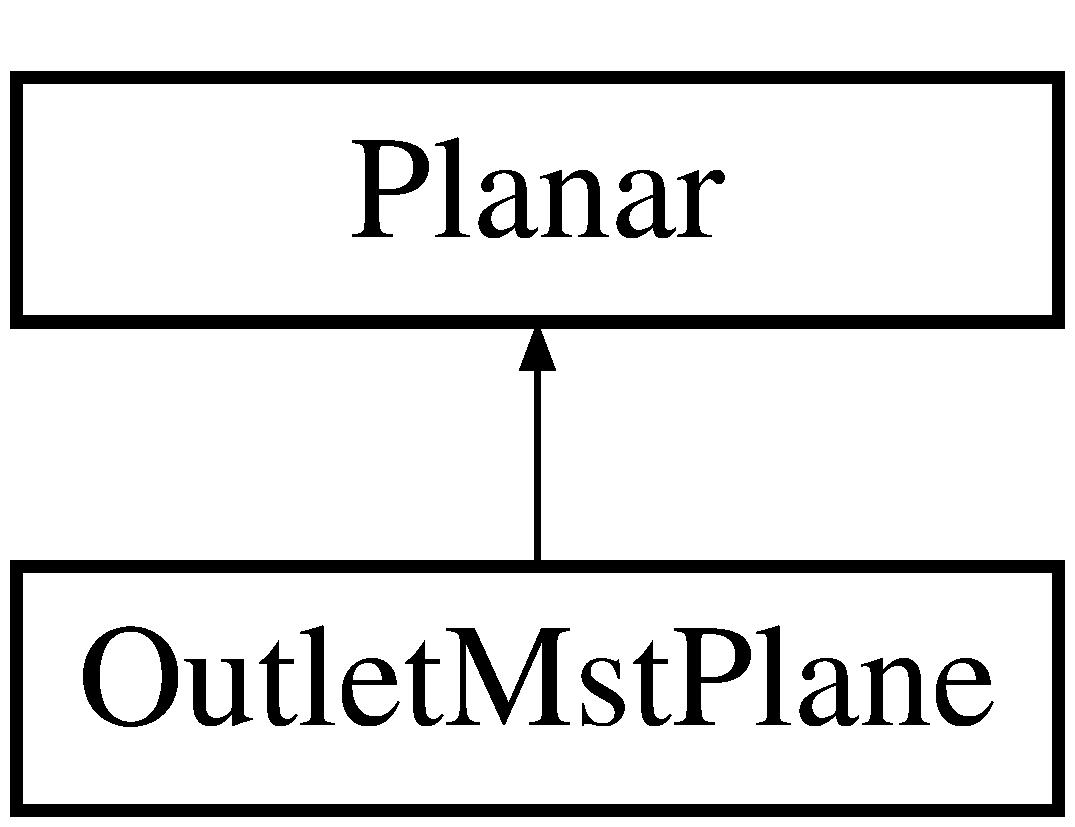
\includegraphics[height=2.000000cm]{d6/de6/class_outlet_mst_plane}
\end{center}
\end{figure}
\subsection*{Public Member Functions}
\begin{DoxyCompactItemize}
\item 
\mbox{\Hypertarget{class_outlet_mst_plane_a83a020ae8e9e225955ff409b0b9e53f6}\label{class_outlet_mst_plane_a83a020ae8e9e225955ff409b0b9e53f6}} 
{\bfseries Outlet\+Mst\+Plane} (double circular\+Duct\+Diameter, double tdx, double pbx, double psx)
\item 
\mbox{\Hypertarget{class_outlet_mst_plane_aa99159d73d39534ac936ad9431503bce}\label{class_outlet_mst_plane_aa99159d73d39534ac936ad9431503bce}} 
{\bfseries Outlet\+Mst\+Plane} (double length, double width, double tdx, double pbx, double psx, unsigned no\+Inlet\+Boxes=1)
\end{DoxyCompactItemize}
\subsection*{Additional Inherited Members}


\subsection{Detailed Description}


Definition at line 76 of file Planar.\+h.



The documentation for this class was generated from the following files\+:\begin{DoxyCompactItemize}
\item 
include/fans/Planar.\+h\item 
src/fans/Planar.\+cpp\end{DoxyCompactItemize}

\hypertarget{struct_compressor_1_1_pipe_sizing_1_1_output}{}\section{Compressor\+:\+:Pipe\+Sizing\+:\+:Output Struct Reference}
\label{struct_compressor_1_1_pipe_sizing_1_1_output}\index{Compressor\+::\+Pipe\+Sizing\+::\+Output@{Compressor\+::\+Pipe\+Sizing\+::\+Output}}
\subsection*{Public Member Functions}
\begin{DoxyCompactItemize}
\item 
\mbox{\Hypertarget{struct_compressor_1_1_pipe_sizing_1_1_output_a30c100e28cf3648c7d0295e6e534dfad}\label{struct_compressor_1_1_pipe_sizing_1_1_output_a30c100e28cf3648c7d0295e6e534dfad}} 
{\bfseries Output} (const double cross\+Sectional\+Area, const double pipe\+Diameter)
\end{DoxyCompactItemize}
\subsection*{Public Attributes}
\begin{DoxyCompactItemize}
\item 
\mbox{\Hypertarget{struct_compressor_1_1_pipe_sizing_1_1_output_ad609e5f5deba43dfb986ece30d93aa27}\label{struct_compressor_1_1_pipe_sizing_1_1_output_ad609e5f5deba43dfb986ece30d93aa27}} 
const double {\bfseries cross\+Sectional\+Area}
\item 
\mbox{\Hypertarget{struct_compressor_1_1_pipe_sizing_1_1_output_ab3a3dcae4259383d06f563a39e617559}\label{struct_compressor_1_1_pipe_sizing_1_1_output_ab3a3dcae4259383d06f563a39e617559}} 
const double {\bfseries pipe\+Diameter}
\end{DoxyCompactItemize}


\subsection{Detailed Description}


Definition at line 288 of file Compressed\+Air.\+h.



The documentation for this struct was generated from the following file\+:\begin{DoxyCompactItemize}
\item 
include/calculator/util/Compressed\+Air.\+h\end{DoxyCompactItemize}

\hypertarget{struct_bag_method_1_1_output}{}\section{Bag\+Method\+:\+:Output Struct Reference}
\label{struct_bag_method_1_1_output}\index{Bag\+Method\+::\+Output@{Bag\+Method\+::\+Output}}
\subsection*{Public Member Functions}
\begin{DoxyCompactItemize}
\item 
\mbox{\Hypertarget{struct_bag_method_1_1_output_a32476edc4a2b924580f0976732cb9aa0}\label{struct_bag_method_1_1_output_a32476edc4a2b924580f0976732cb9aa0}} 
{\bfseries Output} (const double flow\+Rate, const double annual\+Consumption)
\item 
\mbox{\Hypertarget{struct_bag_method_1_1_output_a32476edc4a2b924580f0976732cb9aa0}\label{struct_bag_method_1_1_output_a32476edc4a2b924580f0976732cb9aa0}} 
{\bfseries Output} (const double flow\+Rate, const double annual\+Consumption)
\item 
\mbox{\Hypertarget{struct_bag_method_1_1_output_a32476edc4a2b924580f0976732cb9aa0}\label{struct_bag_method_1_1_output_a32476edc4a2b924580f0976732cb9aa0}} 
{\bfseries Output} (const double flow\+Rate, const double annual\+Consumption)
\end{DoxyCompactItemize}
\subsection*{Public Attributes}
\begin{DoxyCompactItemize}
\item 
\mbox{\Hypertarget{struct_bag_method_1_1_output_a6625c932cfa3935a7198b8ed1747955f}\label{struct_bag_method_1_1_output_a6625c932cfa3935a7198b8ed1747955f}} 
const double {\bfseries flow\+Rate}
\item 
\mbox{\Hypertarget{struct_bag_method_1_1_output_ae287da01450815f1cc6d22b39944482a}\label{struct_bag_method_1_1_output_ae287da01450815f1cc6d22b39944482a}} 
const double {\bfseries annual\+Consumption}
\end{DoxyCompactItemize}


\subsection{Detailed Description}


Definition at line 347 of file Compressed\+Air.\+h.



The documentation for this struct was generated from the following file\+:\begin{DoxyCompactItemize}
\item 
\+\_\+\+C\+Pack\+\_\+\+Packages/\+Darwin/\+S\+T\+G\+Z/amo\+\_\+tools\+\_\+suite-\/-\/\+Darwin-\/x86\+\_\+64-\/\+Debug/amo\+\_\+tools\+\_\+suite/include/calculator/util/Compressed\+Air.\+h\end{DoxyCompactItemize}

\hypertarget{class_pneumatic_air_requirement_1_1_output}{}\section{Pneumatic\+Air\+Requirement\+:\+:Output Class Reference}
\label{class_pneumatic_air_requirement_1_1_output}\index{Pneumatic\+Air\+Requirement\+::\+Output@{Pneumatic\+Air\+Requirement\+::\+Output}}
\subsection*{Public Member Functions}
\begin{DoxyCompactItemize}
\item 
\hyperlink{class_pneumatic_air_requirement_1_1_output_a69397f777ea0aed4b9d3a913883c8a10}{Output} (const double volume\+Air\+Intake\+Piston, const double compression\+Ratio, const double air\+Requirement\+Pneumatic\+Cylinder)
\item 
\hyperlink{class_pneumatic_air_requirement_1_1_output_a69397f777ea0aed4b9d3a913883c8a10}{Output} (const double volume\+Air\+Intake\+Piston, const double compression\+Ratio, const double air\+Requirement\+Pneumatic\+Cylinder)
\item 
\hyperlink{class_pneumatic_air_requirement_1_1_output_a69397f777ea0aed4b9d3a913883c8a10}{Output} (const double volume\+Air\+Intake\+Piston, const double compression\+Ratio, const double air\+Requirement\+Pneumatic\+Cylinder)
\end{DoxyCompactItemize}
\subsection*{Public Attributes}
\begin{DoxyCompactItemize}
\item 
\mbox{\Hypertarget{class_pneumatic_air_requirement_1_1_output_a051ec4d07978c023ba852396e4ae0d0d}\label{class_pneumatic_air_requirement_1_1_output_a051ec4d07978c023ba852396e4ae0d0d}} 
const double {\bfseries volume\+Air\+Intake\+Piston}
\item 
\mbox{\Hypertarget{class_pneumatic_air_requirement_1_1_output_acbf96b686e7226c6c1c5d81b4620c5d8}\label{class_pneumatic_air_requirement_1_1_output_acbf96b686e7226c6c1c5d81b4620c5d8}} 
const double {\bfseries compression\+Ratio}
\item 
\mbox{\Hypertarget{class_pneumatic_air_requirement_1_1_output_a90c33f92f3f215f0b2699ce96f5e845c}\label{class_pneumatic_air_requirement_1_1_output_a90c33f92f3f215f0b2699ce96f5e845c}} 
const double {\bfseries air\+Requirement\+Pneumatic\+Cylinder}
\end{DoxyCompactItemize}


\subsection{Detailed Description}


Definition at line 52 of file Compressed\+Air.\+h.



\subsection{Constructor \& Destructor Documentation}
\mbox{\Hypertarget{class_pneumatic_air_requirement_1_1_output_a69397f777ea0aed4b9d3a913883c8a10}\label{class_pneumatic_air_requirement_1_1_output_a69397f777ea0aed4b9d3a913883c8a10}} 
\index{Pneumatic\+Air\+Requirement\+::\+Output@{Pneumatic\+Air\+Requirement\+::\+Output}!Output@{Output}}
\index{Output@{Output}!Pneumatic\+Air\+Requirement\+::\+Output@{Pneumatic\+Air\+Requirement\+::\+Output}}
\subsubsection{\texorpdfstring{Output()}{Output()}\hspace{0.1cm}{\footnotesize\ttfamily [1/3]}}
{\footnotesize\ttfamily Pneumatic\+Air\+Requirement\+::\+Output\+::\+Output (\begin{DoxyParamCaption}\item[{const double}]{volume\+Air\+Intake\+Piston,  }\item[{const double}]{compression\+Ratio,  }\item[{const double}]{air\+Requirement\+Pneumatic\+Cylinder }\end{DoxyParamCaption})\hspace{0.3cm}{\ttfamily [inline]}}

Constructor for \hyperlink{class_pneumatic_air_requirement_1_1_output}{Pneumatic\+Air\+Requirement\+::\+Output} Used to hold return values 
\begin{DoxyParams}{Parameters}
{\em volume\+Air\+Intake\+Piston} & const double, Volume of air intake in a piston -\/ cubic feet \\
\hline
{\em compression\+Ratio} & const double, The ratio of pressures -\/ Air pressure with atmospheric pressure. \\
\hline
{\em air\+Requirement\+Pneumatic\+Cylinder} & const double, Total cubic feet/min of air requirement for a Pneumatic cylinder -\/ scfm \\
\hline
\end{DoxyParams}


Definition at line 61 of file Compressed\+Air.\+h.

\mbox{\Hypertarget{class_pneumatic_air_requirement_1_1_output_a69397f777ea0aed4b9d3a913883c8a10}\label{class_pneumatic_air_requirement_1_1_output_a69397f777ea0aed4b9d3a913883c8a10}} 
\index{Pneumatic\+Air\+Requirement\+::\+Output@{Pneumatic\+Air\+Requirement\+::\+Output}!Output@{Output}}
\index{Output@{Output}!Pneumatic\+Air\+Requirement\+::\+Output@{Pneumatic\+Air\+Requirement\+::\+Output}}
\subsubsection{\texorpdfstring{Output()}{Output()}\hspace{0.1cm}{\footnotesize\ttfamily [2/3]}}
{\footnotesize\ttfamily Pneumatic\+Air\+Requirement\+::\+Output\+::\+Output (\begin{DoxyParamCaption}\item[{const double}]{volume\+Air\+Intake\+Piston,  }\item[{const double}]{compression\+Ratio,  }\item[{const double}]{air\+Requirement\+Pneumatic\+Cylinder }\end{DoxyParamCaption})\hspace{0.3cm}{\ttfamily [inline]}}

Constructor for \hyperlink{class_pneumatic_air_requirement_1_1_output}{Pneumatic\+Air\+Requirement\+::\+Output} Used to hold return values 
\begin{DoxyParams}{Parameters}
{\em volume\+Air\+Intake\+Piston} & const double, Volume of air intake in a piston -\/ cubic feet \\
\hline
{\em compression\+Ratio} & const double, The ratio of pressures -\/ Air pressure with atmospheric pressure. \\
\hline
{\em air\+Requirement\+Pneumatic\+Cylinder} & const double, Total cubic feet/min of air requirement for a Pneumatic cylinder -\/ scfm \\
\hline
\end{DoxyParams}


Definition at line 61 of file Compressed\+Air.\+h.

\mbox{\Hypertarget{class_pneumatic_air_requirement_1_1_output_a69397f777ea0aed4b9d3a913883c8a10}\label{class_pneumatic_air_requirement_1_1_output_a69397f777ea0aed4b9d3a913883c8a10}} 
\index{Pneumatic\+Air\+Requirement\+::\+Output@{Pneumatic\+Air\+Requirement\+::\+Output}!Output@{Output}}
\index{Output@{Output}!Pneumatic\+Air\+Requirement\+::\+Output@{Pneumatic\+Air\+Requirement\+::\+Output}}
\subsubsection{\texorpdfstring{Output()}{Output()}\hspace{0.1cm}{\footnotesize\ttfamily [3/3]}}
{\footnotesize\ttfamily Pneumatic\+Air\+Requirement\+::\+Output\+::\+Output (\begin{DoxyParamCaption}\item[{const double}]{volume\+Air\+Intake\+Piston,  }\item[{const double}]{compression\+Ratio,  }\item[{const double}]{air\+Requirement\+Pneumatic\+Cylinder }\end{DoxyParamCaption})\hspace{0.3cm}{\ttfamily [inline]}}

Constructor for \hyperlink{class_pneumatic_air_requirement_1_1_output}{Pneumatic\+Air\+Requirement\+::\+Output} Used to hold return values 
\begin{DoxyParams}{Parameters}
{\em volume\+Air\+Intake\+Piston} & const double, Volume of air intake in a piston -\/ cubic feet \\
\hline
{\em compression\+Ratio} & const double, The ratio of pressures -\/ Air pressure with atmospheric pressure. \\
\hline
{\em air\+Requirement\+Pneumatic\+Cylinder} & const double, Total cubic feet/min of air requirement for a Pneumatic cylinder -\/ scfm \\
\hline
\end{DoxyParams}


Definition at line 61 of file Compressed\+Air.\+h.



The documentation for this class was generated from the following file\+:\begin{DoxyCompactItemize}
\item 
\+\_\+\+C\+Pack\+\_\+\+Packages/\+Darwin/\+S\+T\+G\+Z/amo\+\_\+tools\+\_\+suite-\/-\/\+Darwin-\/x86\+\_\+64-\/\+Debug/amo\+\_\+tools\+\_\+suite/include/calculator/util/Compressed\+Air.\+h\end{DoxyCompactItemize}

\hypertarget{struct_compressor_1_1_operating_cost_1_1_output}{}\section{Compressor\+:\+:Operating\+Cost\+:\+:Output Struct Reference}
\label{struct_compressor_1_1_operating_cost_1_1_output}\index{Compressor\+::\+Operating\+Cost\+::\+Output@{Compressor\+::\+Operating\+Cost\+::\+Output}}
\subsection*{Public Member Functions}
\begin{DoxyCompactItemize}
\item 
\mbox{\Hypertarget{struct_compressor_1_1_operating_cost_1_1_output_af510363e57a9f58bdd56f9a16784697e}\label{struct_compressor_1_1_operating_cost_1_1_output_af510363e57a9f58bdd56f9a16784697e}} 
{\bfseries Output} (const double run\+Time\+Unloaded, const double cost\+For\+Loaded, const double cost\+For\+Unloaded, const double total\+Annual\+Cost)
\end{DoxyCompactItemize}
\subsection*{Public Attributes}
\begin{DoxyCompactItemize}
\item 
\mbox{\Hypertarget{struct_compressor_1_1_operating_cost_1_1_output_ae13051fb802def8fc6e18209db38b5aa}\label{struct_compressor_1_1_operating_cost_1_1_output_ae13051fb802def8fc6e18209db38b5aa}} 
const double {\bfseries run\+Time\+Unloaded}
\item 
\mbox{\Hypertarget{struct_compressor_1_1_operating_cost_1_1_output_a4c65ee9ba069d432cf837f42a4702121}\label{struct_compressor_1_1_operating_cost_1_1_output_a4c65ee9ba069d432cf837f42a4702121}} 
const double {\bfseries cost\+For\+Loaded}
\item 
\mbox{\Hypertarget{struct_compressor_1_1_operating_cost_1_1_output_a0e307a677ed5dbf7dba5b061cf5bfccf}\label{struct_compressor_1_1_operating_cost_1_1_output_a0e307a677ed5dbf7dba5b061cf5bfccf}} 
const double {\bfseries cost\+For\+Unloaded}
\item 
\mbox{\Hypertarget{struct_compressor_1_1_operating_cost_1_1_output_a245a4b7baeb985a60d11b65f866563f0}\label{struct_compressor_1_1_operating_cost_1_1_output_a245a4b7baeb985a60d11b65f866563f0}} 
const double {\bfseries total\+Annual\+Cost}
\end{DoxyCompactItemize}


\subsection{Detailed Description}


Definition at line 217 of file Compressed\+Air.\+h.



The documentation for this struct was generated from the following file\+:\begin{DoxyCompactItemize}
\item 
include/calculator/util/Compressed\+Air.\+h\end{DoxyCompactItemize}

\hypertarget{struct_compressor_1_1_air_system_capacity_1_1_output}{}\section{Compressor\+:\+:Air\+System\+Capacity\+:\+:Output Struct Reference}
\label{struct_compressor_1_1_air_system_capacity_1_1_output}\index{Compressor\+::\+Air\+System\+Capacity\+::\+Output@{Compressor\+::\+Air\+System\+Capacity\+::\+Output}}
\subsection*{Public Member Functions}
\begin{DoxyCompactItemize}
\item 
\mbox{\Hypertarget{struct_compressor_1_1_air_system_capacity_1_1_output_ab4065e716b526f38cc310fcec579afde}\label{struct_compressor_1_1_air_system_capacity_1_1_output_ab4065e716b526f38cc310fcec579afde}} 
{\bfseries Output} (const double total\+Pipe\+Volume, std\+::vector$<$ double $>$ receiver\+Capacities, const double total\+Receiver\+Vol, const double total\+Capacity\+Of\+Compressed\+Air\+System, \hyperlink{struct_compressor_1_1_pipe_data}{Pipe\+Data} pipe\+Lengths)
\end{DoxyCompactItemize}
\subsection*{Public Attributes}
\begin{DoxyCompactItemize}
\item 
\mbox{\Hypertarget{struct_compressor_1_1_air_system_capacity_1_1_output_aa6eebf63d38ed5cb2943e6ef0d00d326}\label{struct_compressor_1_1_air_system_capacity_1_1_output_aa6eebf63d38ed5cb2943e6ef0d00d326}} 
const double {\bfseries total\+Pipe\+Volume}
\item 
\mbox{\Hypertarget{struct_compressor_1_1_air_system_capacity_1_1_output_a442171a72537e1c9057f03db3f08a39a}\label{struct_compressor_1_1_air_system_capacity_1_1_output_a442171a72537e1c9057f03db3f08a39a}} 
const double {\bfseries total\+Receiver\+Vol}
\item 
\mbox{\Hypertarget{struct_compressor_1_1_air_system_capacity_1_1_output_a9f81c36e0dfea5574d2e6279b928e288}\label{struct_compressor_1_1_air_system_capacity_1_1_output_a9f81c36e0dfea5574d2e6279b928e288}} 
const double {\bfseries total\+Capacity\+Of\+Compressed\+Air\+System}
\item 
\mbox{\Hypertarget{struct_compressor_1_1_air_system_capacity_1_1_output_abb4c6d9da5e99160ca9ee8fc1b41a311}\label{struct_compressor_1_1_air_system_capacity_1_1_output_abb4c6d9da5e99160ca9ee8fc1b41a311}} 
const std\+::vector$<$ double $>$ {\bfseries receiver\+Capacities}
\item 
\mbox{\Hypertarget{struct_compressor_1_1_air_system_capacity_1_1_output_a1a2fe0406a4ff682d7141df7b5e4b150}\label{struct_compressor_1_1_air_system_capacity_1_1_output_a1a2fe0406a4ff682d7141df7b5e4b150}} 
const \hyperlink{struct_compressor_1_1_pipe_data}{Pipe\+Data} {\bfseries pipe\+Lengths}
\end{DoxyCompactItemize}


\subsection{Detailed Description}


Definition at line 239 of file Compressed\+Air.\+h.



The documentation for this struct was generated from the following file\+:\begin{DoxyCompactItemize}
\item 
include/calculator/util/Compressed\+Air.\+h\end{DoxyCompactItemize}

\hypertarget{struct_compressor_1_1_pipe_data}{}\section{Compressor\+:\+:Pipe\+Data Struct Reference}
\label{struct_compressor_1_1_pipe_data}\index{Compressor\+::\+Pipe\+Data@{Compressor\+::\+Pipe\+Data}}
\subsection*{Public Member Functions}
\begin{DoxyCompactItemize}
\item 
\hyperlink{struct_compressor_1_1_pipe_data_a71acdc81e25bd90b51361bf8d4f0ed38}{Pipe\+Data} (const double one\+Half, const double three\+Fourths, const double one, const double one\+And\+One\+Fourth, const double one\+And\+One\+Half, const double two, const double two\+And\+One\+Half, const double three, const double three\+And\+One\+Half, const double four, const double five, const double six)
\item 
\hyperlink{struct_compressor_1_1_pipe_data_af7998fd533340b0a84e78fcda91b4806}{Pipe\+Data} (std\+::function$<$ double(const double)$>$ const \&comp\+Vel)
\item 
\hyperlink{struct_compressor_1_1_pipe_data_a71acdc81e25bd90b51361bf8d4f0ed38}{Pipe\+Data} (const double one\+Half, const double three\+Fourths, const double one, const double one\+And\+One\+Fourth, const double one\+And\+One\+Half, const double two, const double two\+And\+One\+Half, const double three, const double three\+And\+One\+Half, const double four, const double five, const double six)
\item 
\hyperlink{struct_compressor_1_1_pipe_data_af7998fd533340b0a84e78fcda91b4806}{Pipe\+Data} (std\+::function$<$ double(const double)$>$ const \&comp\+Vel)
\item 
\hyperlink{struct_compressor_1_1_pipe_data_a71acdc81e25bd90b51361bf8d4f0ed38}{Pipe\+Data} (const double one\+Half, const double three\+Fourths, const double one, const double one\+And\+One\+Fourth, const double one\+And\+One\+Half, const double two, const double two\+And\+One\+Half, const double three, const double three\+And\+One\+Half, const double four, const double five, const double six)
\item 
\hyperlink{struct_compressor_1_1_pipe_data_af7998fd533340b0a84e78fcda91b4806}{Pipe\+Data} (std\+::function$<$ double(const double)$>$ const \&comp\+Vel)
\end{DoxyCompactItemize}
\subsection*{Public Attributes}
\begin{DoxyCompactItemize}
\item 
\mbox{\Hypertarget{struct_compressor_1_1_pipe_data_a7236f0b12e200de8e46f637df3352d0d}\label{struct_compressor_1_1_pipe_data_a7236f0b12e200de8e46f637df3352d0d}} 
const double {\bfseries one\+Half}
\item 
\mbox{\Hypertarget{struct_compressor_1_1_pipe_data_ab48dcf529d0206f4bb0fa2cc828b4dc0}\label{struct_compressor_1_1_pipe_data_ab48dcf529d0206f4bb0fa2cc828b4dc0}} 
const double {\bfseries three\+Fourths}
\item 
\mbox{\Hypertarget{struct_compressor_1_1_pipe_data_a884c2f008f0057d4f94c0742e4dd3c3b}\label{struct_compressor_1_1_pipe_data_a884c2f008f0057d4f94c0742e4dd3c3b}} 
const double {\bfseries one}
\item 
\mbox{\Hypertarget{struct_compressor_1_1_pipe_data_ad790420771f56d18e0d34c0a6ac512cd}\label{struct_compressor_1_1_pipe_data_ad790420771f56d18e0d34c0a6ac512cd}} 
const double {\bfseries one\+And\+One\+Fourth}
\item 
\mbox{\Hypertarget{struct_compressor_1_1_pipe_data_a4971263590f68f45e9848f812d3dd5e9}\label{struct_compressor_1_1_pipe_data_a4971263590f68f45e9848f812d3dd5e9}} 
const double {\bfseries one\+And\+One\+Half}
\item 
\mbox{\Hypertarget{struct_compressor_1_1_pipe_data_aa4d140783f97964786ece8ad272fc829}\label{struct_compressor_1_1_pipe_data_aa4d140783f97964786ece8ad272fc829}} 
const double {\bfseries two}
\item 
\mbox{\Hypertarget{struct_compressor_1_1_pipe_data_ae57d992a97e54352f79868e9fa89c369}\label{struct_compressor_1_1_pipe_data_ae57d992a97e54352f79868e9fa89c369}} 
const double {\bfseries two\+And\+One\+Half}
\item 
\mbox{\Hypertarget{struct_compressor_1_1_pipe_data_ab0d1b23638ec83752755eac2d04cae85}\label{struct_compressor_1_1_pipe_data_ab0d1b23638ec83752755eac2d04cae85}} 
const double {\bfseries three}
\item 
\mbox{\Hypertarget{struct_compressor_1_1_pipe_data_a6dbfd92e9cb49a8bb470ef74cb871dcf}\label{struct_compressor_1_1_pipe_data_a6dbfd92e9cb49a8bb470ef74cb871dcf}} 
const double {\bfseries three\+And\+One\+Half}
\item 
\mbox{\Hypertarget{struct_compressor_1_1_pipe_data_a0a73b41257d2ed6e91b1a06833e5cd65}\label{struct_compressor_1_1_pipe_data_a0a73b41257d2ed6e91b1a06833e5cd65}} 
const double {\bfseries four}
\item 
\mbox{\Hypertarget{struct_compressor_1_1_pipe_data_aa4ca33456ade4559b80bdc55d785ca12}\label{struct_compressor_1_1_pipe_data_aa4ca33456ade4559b80bdc55d785ca12}} 
const double {\bfseries five}
\item 
\mbox{\Hypertarget{struct_compressor_1_1_pipe_data_acabd73fa371dec551937b5d9f7718317}\label{struct_compressor_1_1_pipe_data_acabd73fa371dec551937b5d9f7718317}} 
const double {\bfseries six}
\item 
\mbox{\Hypertarget{struct_compressor_1_1_pipe_data_aa290d5d7f31c6b74f65b22d81b4ebf84}\label{struct_compressor_1_1_pipe_data_aa290d5d7f31c6b74f65b22d81b4ebf84}} 
const double {\bfseries total\+Pipe\+Volume} = 0
\end{DoxyCompactItemize}


\subsection{Detailed Description}


Definition at line 164 of file Compressed\+Air.\+h.



\subsection{Constructor \& Destructor Documentation}
\mbox{\Hypertarget{struct_compressor_1_1_pipe_data_a71acdc81e25bd90b51361bf8d4f0ed38}\label{struct_compressor_1_1_pipe_data_a71acdc81e25bd90b51361bf8d4f0ed38}} 
\index{Compressor\+::\+Pipe\+Data@{Compressor\+::\+Pipe\+Data}!Pipe\+Data@{Pipe\+Data}}
\index{Pipe\+Data@{Pipe\+Data}!Compressor\+::\+Pipe\+Data@{Compressor\+::\+Pipe\+Data}}
\subsubsection{\texorpdfstring{Pipe\+Data()}{PipeData()}\hspace{0.1cm}{\footnotesize\ttfamily [1/6]}}
{\footnotesize\ttfamily Compressor\+::\+Pipe\+Data\+::\+Pipe\+Data (\begin{DoxyParamCaption}\item[{const double}]{one\+Half,  }\item[{const double}]{three\+Fourths,  }\item[{const double}]{one,  }\item[{const double}]{one\+And\+One\+Fourth,  }\item[{const double}]{one\+And\+One\+Half,  }\item[{const double}]{two,  }\item[{const double}]{two\+And\+One\+Half,  }\item[{const double}]{three,  }\item[{const double}]{three\+And\+One\+Half,  }\item[{const double}]{four,  }\item[{const double}]{five,  }\item[{const double}]{six }\end{DoxyParamCaption})\hspace{0.3cm}{\ttfamily [inline]}}

Constructor for \hyperlink{struct_compressor_1_1_pipe_data}{Compressor\+::\+Pipe\+Data} -\/ This is used to hold all the pipe lengths in the system All params are the english spelling of their numeric equivalents, i.\+e. one half == 0.\+5, two\+And\+One\+Half == 2.\+5, etc. Used in \hyperlink{class_compressor_1_1_air_system_capacity}{Air\+System\+Capacity} input and output. 

Definition at line 170 of file Compressed\+Air.\+h.

\mbox{\Hypertarget{struct_compressor_1_1_pipe_data_af7998fd533340b0a84e78fcda91b4806}\label{struct_compressor_1_1_pipe_data_af7998fd533340b0a84e78fcda91b4806}} 
\index{Compressor\+::\+Pipe\+Data@{Compressor\+::\+Pipe\+Data}!Pipe\+Data@{Pipe\+Data}}
\index{Pipe\+Data@{Pipe\+Data}!Compressor\+::\+Pipe\+Data@{Compressor\+::\+Pipe\+Data}}
\subsubsection{\texorpdfstring{Pipe\+Data()}{PipeData()}\hspace{0.1cm}{\footnotesize\ttfamily [2/6]}}
{\footnotesize\ttfamily Compressor\+::\+Pipe\+Data\+::\+Pipe\+Data (\begin{DoxyParamCaption}\item[{std\+::function$<$ double(const double)$>$ const \&}]{comp\+Vel }\end{DoxyParamCaption})\hspace{0.3cm}{\ttfamily [inline]}, {\ttfamily [explicit]}}

Constructor for \hyperlink{struct_compressor_1_1_pipe_data}{Compressor\+::\+Pipe\+Data} -\/ This is used to hold return values for air velocity estimations 
\begin{DoxyParams}{Parameters}
{\em comp\+Vel} & std\+::function$<$double (const double)$>$, comp\+Vel is the compressed air velocity function, it calculates pipeline velocity given internal area of the pipe in square feet. An example of usage can be found in Air\+Velocity\+::calculate() \\
\hline
\end{DoxyParams}


Definition at line 189 of file Compressed\+Air.\+h.

\mbox{\Hypertarget{struct_compressor_1_1_pipe_data_a71acdc81e25bd90b51361bf8d4f0ed38}\label{struct_compressor_1_1_pipe_data_a71acdc81e25bd90b51361bf8d4f0ed38}} 
\index{Compressor\+::\+Pipe\+Data@{Compressor\+::\+Pipe\+Data}!Pipe\+Data@{Pipe\+Data}}
\index{Pipe\+Data@{Pipe\+Data}!Compressor\+::\+Pipe\+Data@{Compressor\+::\+Pipe\+Data}}
\subsubsection{\texorpdfstring{Pipe\+Data()}{PipeData()}\hspace{0.1cm}{\footnotesize\ttfamily [3/6]}}
{\footnotesize\ttfamily Compressor\+::\+Pipe\+Data\+::\+Pipe\+Data (\begin{DoxyParamCaption}\item[{const double}]{one\+Half,  }\item[{const double}]{three\+Fourths,  }\item[{const double}]{one,  }\item[{const double}]{one\+And\+One\+Fourth,  }\item[{const double}]{one\+And\+One\+Half,  }\item[{const double}]{two,  }\item[{const double}]{two\+And\+One\+Half,  }\item[{const double}]{three,  }\item[{const double}]{three\+And\+One\+Half,  }\item[{const double}]{four,  }\item[{const double}]{five,  }\item[{const double}]{six }\end{DoxyParamCaption})\hspace{0.3cm}{\ttfamily [inline]}}

Constructor for \hyperlink{struct_compressor_1_1_pipe_data}{Compressor\+::\+Pipe\+Data} -\/ This is used to hold all the pipe lengths in the system All params are the english spelling of their numeric equivalents, i.\+e. one half == 0.\+5, two\+And\+One\+Half == 2.\+5, etc. Used in \hyperlink{class_compressor_1_1_air_system_capacity}{Air\+System\+Capacity} input and output. 

Definition at line 170 of file Compressed\+Air.\+h.

\mbox{\Hypertarget{struct_compressor_1_1_pipe_data_af7998fd533340b0a84e78fcda91b4806}\label{struct_compressor_1_1_pipe_data_af7998fd533340b0a84e78fcda91b4806}} 
\index{Compressor\+::\+Pipe\+Data@{Compressor\+::\+Pipe\+Data}!Pipe\+Data@{Pipe\+Data}}
\index{Pipe\+Data@{Pipe\+Data}!Compressor\+::\+Pipe\+Data@{Compressor\+::\+Pipe\+Data}}
\subsubsection{\texorpdfstring{Pipe\+Data()}{PipeData()}\hspace{0.1cm}{\footnotesize\ttfamily [4/6]}}
{\footnotesize\ttfamily Compressor\+::\+Pipe\+Data\+::\+Pipe\+Data (\begin{DoxyParamCaption}\item[{std\+::function$<$ double(const double)$>$ const \&}]{comp\+Vel }\end{DoxyParamCaption})\hspace{0.3cm}{\ttfamily [inline]}, {\ttfamily [explicit]}}

Constructor for \hyperlink{struct_compressor_1_1_pipe_data}{Compressor\+::\+Pipe\+Data} -\/ This is used to hold return values for air velocity estimations 
\begin{DoxyParams}{Parameters}
{\em comp\+Vel} & std\+::function$<$double (const double)$>$, comp\+Vel is the compressed air velocity function, it calculates pipeline velocity given internal area of the pipe in square feet. An example of usage can be found in Air\+Velocity\+::calculate() \\
\hline
\end{DoxyParams}


Definition at line 189 of file Compressed\+Air.\+h.

\mbox{\Hypertarget{struct_compressor_1_1_pipe_data_a71acdc81e25bd90b51361bf8d4f0ed38}\label{struct_compressor_1_1_pipe_data_a71acdc81e25bd90b51361bf8d4f0ed38}} 
\index{Compressor\+::\+Pipe\+Data@{Compressor\+::\+Pipe\+Data}!Pipe\+Data@{Pipe\+Data}}
\index{Pipe\+Data@{Pipe\+Data}!Compressor\+::\+Pipe\+Data@{Compressor\+::\+Pipe\+Data}}
\subsubsection{\texorpdfstring{Pipe\+Data()}{PipeData()}\hspace{0.1cm}{\footnotesize\ttfamily [5/6]}}
{\footnotesize\ttfamily Compressor\+::\+Pipe\+Data\+::\+Pipe\+Data (\begin{DoxyParamCaption}\item[{const double}]{one\+Half,  }\item[{const double}]{three\+Fourths,  }\item[{const double}]{one,  }\item[{const double}]{one\+And\+One\+Fourth,  }\item[{const double}]{one\+And\+One\+Half,  }\item[{const double}]{two,  }\item[{const double}]{two\+And\+One\+Half,  }\item[{const double}]{three,  }\item[{const double}]{three\+And\+One\+Half,  }\item[{const double}]{four,  }\item[{const double}]{five,  }\item[{const double}]{six }\end{DoxyParamCaption})\hspace{0.3cm}{\ttfamily [inline]}}

Constructor for \hyperlink{struct_compressor_1_1_pipe_data}{Compressor\+::\+Pipe\+Data} -\/ This is used to hold all the pipe lengths in the system All params are the english spelling of their numeric equivalents, i.\+e. one half == 0.\+5, two\+And\+One\+Half == 2.\+5, etc. Used in \hyperlink{class_compressor_1_1_air_system_capacity}{Air\+System\+Capacity} input and output. 

Definition at line 170 of file Compressed\+Air.\+h.

\mbox{\Hypertarget{struct_compressor_1_1_pipe_data_af7998fd533340b0a84e78fcda91b4806}\label{struct_compressor_1_1_pipe_data_af7998fd533340b0a84e78fcda91b4806}} 
\index{Compressor\+::\+Pipe\+Data@{Compressor\+::\+Pipe\+Data}!Pipe\+Data@{Pipe\+Data}}
\index{Pipe\+Data@{Pipe\+Data}!Compressor\+::\+Pipe\+Data@{Compressor\+::\+Pipe\+Data}}
\subsubsection{\texorpdfstring{Pipe\+Data()}{PipeData()}\hspace{0.1cm}{\footnotesize\ttfamily [6/6]}}
{\footnotesize\ttfamily Compressor\+::\+Pipe\+Data\+::\+Pipe\+Data (\begin{DoxyParamCaption}\item[{std\+::function$<$ double(const double)$>$ const \&}]{comp\+Vel }\end{DoxyParamCaption})\hspace{0.3cm}{\ttfamily [inline]}, {\ttfamily [explicit]}}

Constructor for \hyperlink{struct_compressor_1_1_pipe_data}{Compressor\+::\+Pipe\+Data} -\/ This is used to hold return values for air velocity estimations 
\begin{DoxyParams}{Parameters}
{\em comp\+Vel} & std\+::function$<$double (const double)$>$, comp\+Vel is the compressed air velocity function, it calculates pipeline velocity given internal area of the pipe in square feet. An example of usage can be found in Air\+Velocity\+::calculate() \\
\hline
\end{DoxyParams}


Definition at line 189 of file Compressed\+Air.\+h.



The documentation for this struct was generated from the following file\+:\begin{DoxyCompactItemize}
\item 
\+\_\+\+C\+Pack\+\_\+\+Packages/\+Darwin/\+S\+T\+G\+Z/amo\+\_\+tools\+\_\+suite-\/-\/\+Darwin-\/x86\+\_\+64/amo\+\_\+tools\+\_\+suite/include/calculator/util/Compressed\+Air.\+h\end{DoxyCompactItemize}

\hypertarget{class_compressor_1_1_pipe_sizing}{}\section{Compressor\+:\+:Pipe\+Sizing Class Reference}
\label{class_compressor_1_1_pipe_sizing}\index{Compressor\+::\+Pipe\+Sizing@{Compressor\+::\+Pipe\+Sizing}}
\subsection*{Classes}
\begin{DoxyCompactItemize}
\item 
struct \hyperlink{struct_compressor_1_1_pipe_sizing_1_1_output}{Output}
\end{DoxyCompactItemize}
\subsection*{Public Member Functions}
\begin{DoxyCompactItemize}
\item 
\hyperlink{class_compressor_1_1_pipe_sizing_a63d7a8e0780e80938489f160b5996abb}{Pipe\+Sizing} (double airflow, double airline\+Pressure, double design\+Velocity, double atmospheric\+Pressure)
\item 
\hyperlink{struct_compressor_1_1_pipe_sizing_1_1_output}{Output} \hyperlink{class_compressor_1_1_pipe_sizing_a9212c8d52ff658c412752cee18d6b28d}{calculate} ()
\item 
\hyperlink{class_compressor_1_1_pipe_sizing_a63d7a8e0780e80938489f160b5996abb}{Pipe\+Sizing} (double airflow, double airline\+Pressure, double design\+Velocity, double atmospheric\+Pressure)
\item 
\hyperlink{struct_compressor_1_1_pipe_sizing_1_1_output}{Output} \hyperlink{class_compressor_1_1_pipe_sizing_a0b4a10531fb9a8c3bb9aae0441ed5182}{calculate} ()
\item 
\hyperlink{class_compressor_1_1_pipe_sizing_a63d7a8e0780e80938489f160b5996abb}{Pipe\+Sizing} (double airflow, double airline\+Pressure, double design\+Velocity, double atmospheric\+Pressure)
\item 
\hyperlink{struct_compressor_1_1_pipe_sizing_1_1_output}{Output} \hyperlink{class_compressor_1_1_pipe_sizing_a0b4a10531fb9a8c3bb9aae0441ed5182}{calculate} ()
\end{DoxyCompactItemize}


\subsection{Detailed Description}


Definition at line 288 of file Compressed\+Air.\+h.



\subsection{Constructor \& Destructor Documentation}
\mbox{\Hypertarget{class_compressor_1_1_pipe_sizing_a63d7a8e0780e80938489f160b5996abb}\label{class_compressor_1_1_pipe_sizing_a63d7a8e0780e80938489f160b5996abb}} 
\index{Compressor\+::\+Pipe\+Sizing@{Compressor\+::\+Pipe\+Sizing}!Pipe\+Sizing@{Pipe\+Sizing}}
\index{Pipe\+Sizing@{Pipe\+Sizing}!Compressor\+::\+Pipe\+Sizing@{Compressor\+::\+Pipe\+Sizing}}
\subsubsection{\texorpdfstring{Pipe\+Sizing()}{PipeSizing()}\hspace{0.1cm}{\footnotesize\ttfamily [1/3]}}
{\footnotesize\ttfamily Compressor\+::\+Pipe\+Sizing\+::\+Pipe\+Sizing (\begin{DoxyParamCaption}\item[{double}]{airflow,  }\item[{double}]{airline\+Pressure,  }\item[{double}]{design\+Velocity,  }\item[{double}]{atmospheric\+Pressure }\end{DoxyParamCaption})}

Constructor for \hyperlink{class_compressor_1_1_pipe_sizing}{Compressor\+::\+Pipe\+Sizing} -\/ This calculator finds the velocity of compressed air through all the different piping involved in the system. 
\begin{DoxyParams}{Parameters}
{\em airflow} & double, volumetric flow velocity -\/ cfm \\
\hline
{\em airline\+Pressure} & double, Pressure through the pipe -\/ psi \\
\hline
{\em design\+Velocity} & double, The air flow velocity that is meant to flow through the pipe. \\
\hline
\end{DoxyParams}
\begin{DoxyAttention}{Attention}
Constraints\+: 20 fps is recommended for a header, but it should never exceed 30 fps -\/ ft/sc 
\end{DoxyAttention}

\begin{DoxyParams}{Parameters}
{\em atmospheric\+Pressure} & double, generally it will be 14.\+7 -\/ psia \\
\hline
\end{DoxyParams}


Definition at line 132 of file Compressed\+Air.\+cpp.

\mbox{\Hypertarget{class_compressor_1_1_pipe_sizing_a63d7a8e0780e80938489f160b5996abb}\label{class_compressor_1_1_pipe_sizing_a63d7a8e0780e80938489f160b5996abb}} 
\index{Compressor\+::\+Pipe\+Sizing@{Compressor\+::\+Pipe\+Sizing}!Pipe\+Sizing@{Pipe\+Sizing}}
\index{Pipe\+Sizing@{Pipe\+Sizing}!Compressor\+::\+Pipe\+Sizing@{Compressor\+::\+Pipe\+Sizing}}
\subsubsection{\texorpdfstring{Pipe\+Sizing()}{PipeSizing()}\hspace{0.1cm}{\footnotesize\ttfamily [2/3]}}
{\footnotesize\ttfamily Compressor\+::\+Pipe\+Sizing\+::\+Pipe\+Sizing (\begin{DoxyParamCaption}\item[{double}]{airflow,  }\item[{double}]{airline\+Pressure,  }\item[{double}]{design\+Velocity,  }\item[{double}]{atmospheric\+Pressure }\end{DoxyParamCaption})}

Constructor for \hyperlink{class_compressor_1_1_pipe_sizing}{Compressor\+::\+Pipe\+Sizing} -\/ This calculator finds the velocity of compressed air through all the different piping involved in the system. 
\begin{DoxyParams}{Parameters}
{\em airflow} & double, volumetric flow velocity -\/ cfm \\
\hline
{\em airline\+Pressure} & double, Pressure through the pipe -\/ psi \\
\hline
{\em design\+Velocity} & double, The air flow velocity that is meant to flow through the pipe. \\
\hline
\end{DoxyParams}
\begin{DoxyAttention}{Attention}
Constraints\+: 20 fps is recommended for a header, but it should never exceed 30 fps -\/ ft/sc 
\end{DoxyAttention}

\begin{DoxyParams}{Parameters}
{\em atmospheric\+Pressure} & double, generally it will be 14.\+7 -\/ psia \\
\hline
\end{DoxyParams}
\mbox{\Hypertarget{class_compressor_1_1_pipe_sizing_a63d7a8e0780e80938489f160b5996abb}\label{class_compressor_1_1_pipe_sizing_a63d7a8e0780e80938489f160b5996abb}} 
\index{Compressor\+::\+Pipe\+Sizing@{Compressor\+::\+Pipe\+Sizing}!Pipe\+Sizing@{Pipe\+Sizing}}
\index{Pipe\+Sizing@{Pipe\+Sizing}!Compressor\+::\+Pipe\+Sizing@{Compressor\+::\+Pipe\+Sizing}}
\subsubsection{\texorpdfstring{Pipe\+Sizing()}{PipeSizing()}\hspace{0.1cm}{\footnotesize\ttfamily [3/3]}}
{\footnotesize\ttfamily Compressor\+::\+Pipe\+Sizing\+::\+Pipe\+Sizing (\begin{DoxyParamCaption}\item[{double}]{airflow,  }\item[{double}]{airline\+Pressure,  }\item[{double}]{design\+Velocity,  }\item[{double}]{atmospheric\+Pressure }\end{DoxyParamCaption})}

Constructor for \hyperlink{class_compressor_1_1_pipe_sizing}{Compressor\+::\+Pipe\+Sizing} -\/ This calculator finds the velocity of compressed air through all the different piping involved in the system. 
\begin{DoxyParams}{Parameters}
{\em airflow} & double, volumetric flow velocity -\/ cfm \\
\hline
{\em airline\+Pressure} & double, Pressure through the pipe -\/ psi \\
\hline
{\em design\+Velocity} & double, The air flow velocity that is meant to flow through the pipe. \\
\hline
\end{DoxyParams}
\begin{DoxyAttention}{Attention}
Constraints\+: 20 fps is recommended for a header, but it should never exceed 30 fps -\/ ft/sc 
\end{DoxyAttention}

\begin{DoxyParams}{Parameters}
{\em atmospheric\+Pressure} & double, generally it will be 14.\+7 -\/ psia \\
\hline
\end{DoxyParams}


\subsection{Member Function Documentation}
\mbox{\Hypertarget{class_compressor_1_1_pipe_sizing_a9212c8d52ff658c412752cee18d6b28d}\label{class_compressor_1_1_pipe_sizing_a9212c8d52ff658c412752cee18d6b28d}} 
\index{Compressor\+::\+Pipe\+Sizing@{Compressor\+::\+Pipe\+Sizing}!calculate@{calculate}}
\index{calculate@{calculate}!Compressor\+::\+Pipe\+Sizing@{Compressor\+::\+Pipe\+Sizing}}
\subsubsection{\texorpdfstring{calculate()}{calculate()}\hspace{0.1cm}{\footnotesize\ttfamily [1/3]}}
{\footnotesize\ttfamily \hyperlink{struct_compressor_1_1_pipe_sizing_1_1_output}{Compressor\+::\+Pipe\+Sizing\+::\+Output} Compressor\+::\+Pipe\+Sizing\+::calculate (\begin{DoxyParamCaption}{ }\end{DoxyParamCaption})}

\hyperlink{class_compressor_1_1_pipe_sizing_a9212c8d52ff658c412752cee18d6b28d}{calculate()} will calculate and return the cross sectional area and the pipe diameter. \begin{DoxyReturn}{Returns}
\hyperlink{struct_compressor_1_1_pipe_sizing_1_1_output}{Pipe\+Sizing\+::\+Output} 
\end{DoxyReturn}


Definition at line 138 of file Compressed\+Air.\+cpp.

\mbox{\Hypertarget{class_compressor_1_1_pipe_sizing_a0b4a10531fb9a8c3bb9aae0441ed5182}\label{class_compressor_1_1_pipe_sizing_a0b4a10531fb9a8c3bb9aae0441ed5182}} 
\index{Compressor\+::\+Pipe\+Sizing@{Compressor\+::\+Pipe\+Sizing}!calculate@{calculate}}
\index{calculate@{calculate}!Compressor\+::\+Pipe\+Sizing@{Compressor\+::\+Pipe\+Sizing}}
\subsubsection{\texorpdfstring{calculate()}{calculate()}\hspace{0.1cm}{\footnotesize\ttfamily [2/3]}}
{\footnotesize\ttfamily \hyperlink{struct_compressor_1_1_pipe_sizing_1_1_output}{Output} Compressor\+::\+Pipe\+Sizing\+::calculate (\begin{DoxyParamCaption}{ }\end{DoxyParamCaption})}

\hyperlink{class_compressor_1_1_pipe_sizing_a9212c8d52ff658c412752cee18d6b28d}{calculate()} will calculate and return the cross sectional area and the pipe diameter. \begin{DoxyReturn}{Returns}
\hyperlink{struct_compressor_1_1_pipe_sizing_1_1_output}{Pipe\+Sizing\+::\+Output} 
\end{DoxyReturn}
\mbox{\Hypertarget{class_compressor_1_1_pipe_sizing_a0b4a10531fb9a8c3bb9aae0441ed5182}\label{class_compressor_1_1_pipe_sizing_a0b4a10531fb9a8c3bb9aae0441ed5182}} 
\index{Compressor\+::\+Pipe\+Sizing@{Compressor\+::\+Pipe\+Sizing}!calculate@{calculate}}
\index{calculate@{calculate}!Compressor\+::\+Pipe\+Sizing@{Compressor\+::\+Pipe\+Sizing}}
\subsubsection{\texorpdfstring{calculate()}{calculate()}\hspace{0.1cm}{\footnotesize\ttfamily [3/3]}}
{\footnotesize\ttfamily \hyperlink{struct_compressor_1_1_pipe_sizing_1_1_output}{Output} Compressor\+::\+Pipe\+Sizing\+::calculate (\begin{DoxyParamCaption}{ }\end{DoxyParamCaption})}

\hyperlink{class_compressor_1_1_pipe_sizing_a9212c8d52ff658c412752cee18d6b28d}{calculate()} will calculate and return the cross sectional area and the pipe diameter. \begin{DoxyReturn}{Returns}
\hyperlink{struct_compressor_1_1_pipe_sizing_1_1_output}{Pipe\+Sizing\+::\+Output} 
\end{DoxyReturn}


The documentation for this class was generated from the following files\+:\begin{DoxyCompactItemize}
\item 
\+\_\+\+C\+Pack\+\_\+\+Packages/\+Darwin/\+S\+T\+G\+Z/amo\+\_\+tools\+\_\+suite-\/-\/\+Darwin-\/x86\+\_\+64/amo\+\_\+tools\+\_\+suite/include/calculator/util/Compressed\+Air.\+h\item 
src/calculator/util/Compressed\+Air.\+cpp\end{DoxyCompactItemize}

\hypertarget{class_planar}{}\section{Planar Class Reference}
\label{class_planar}\index{Planar@{Planar}}
Inheritance diagram for Planar\+:\begin{figure}[H]
\begin{center}
\leavevmode
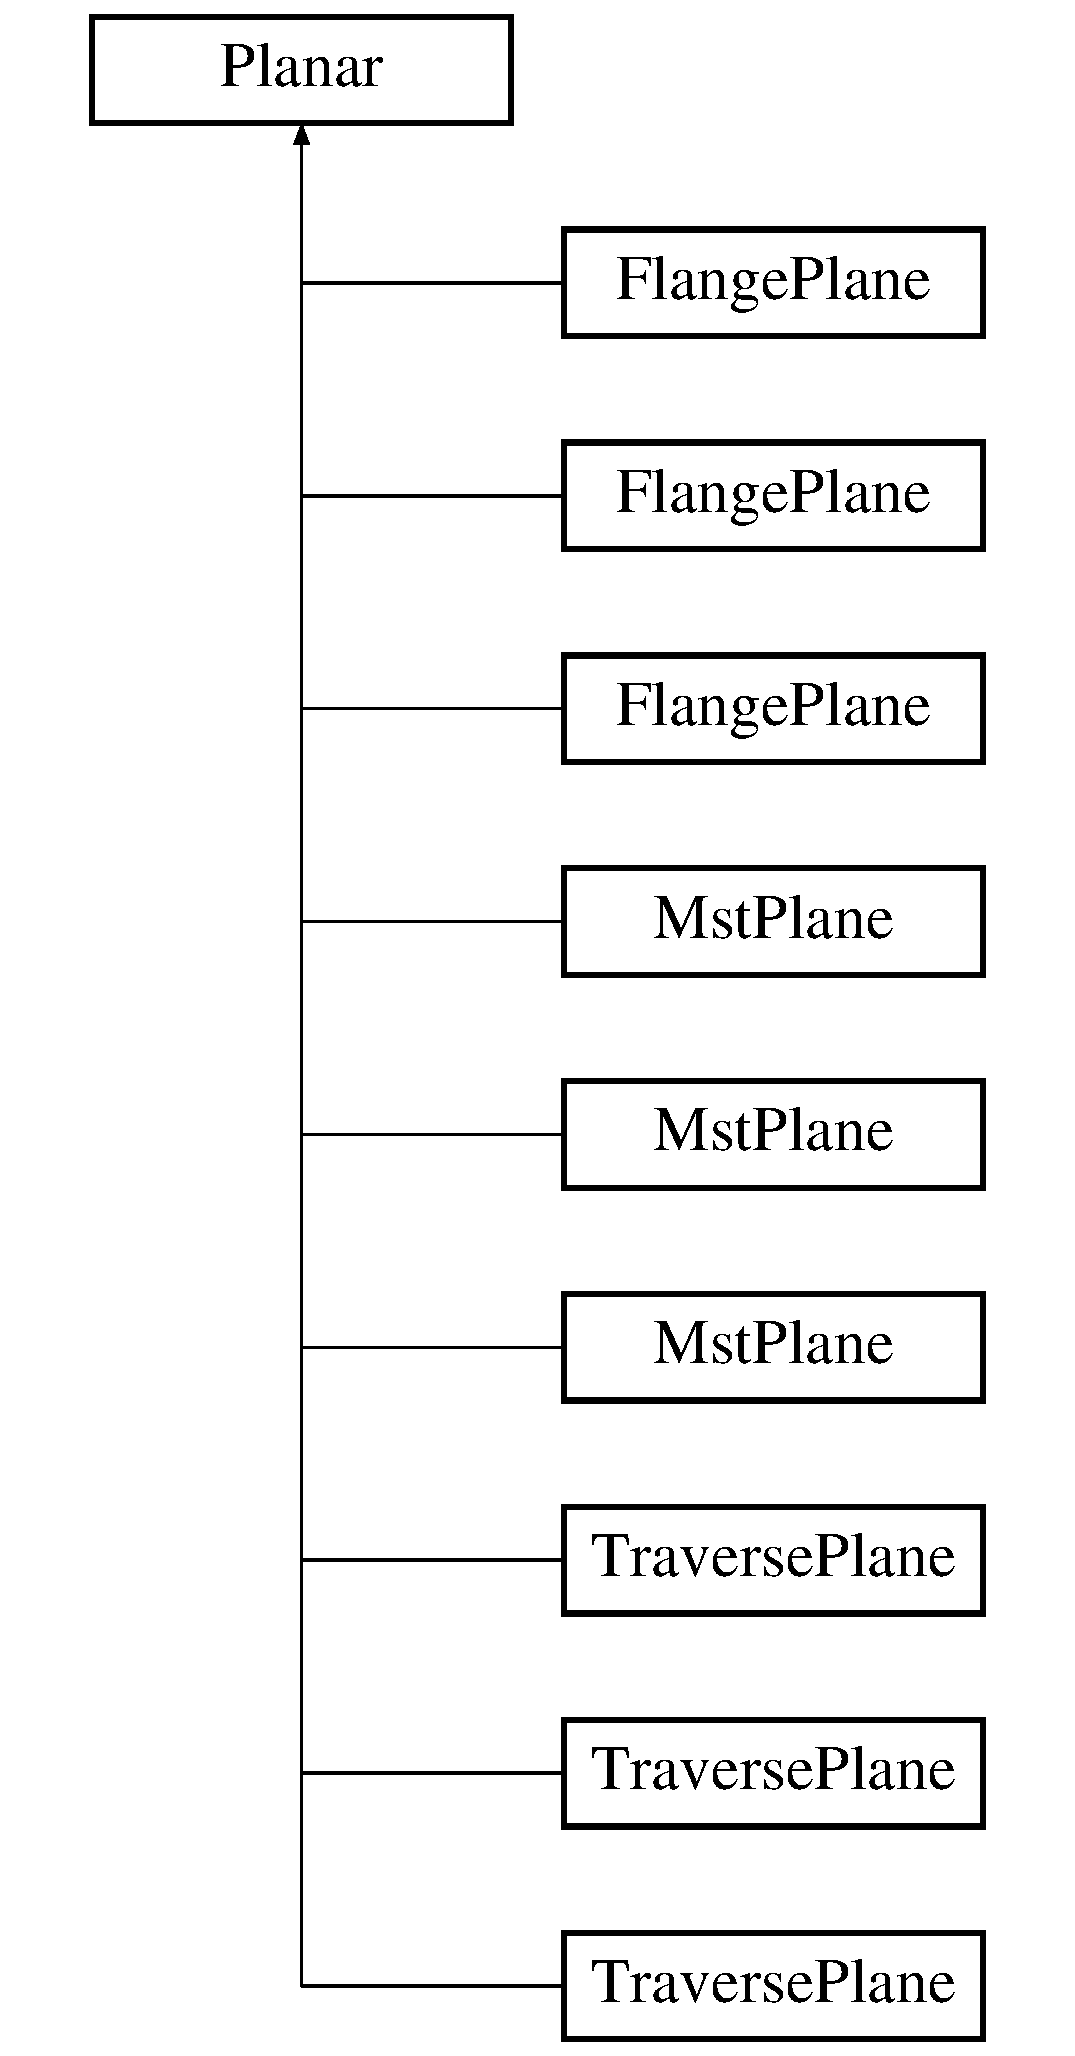
\includegraphics[height=10.000000cm]{d2/ddc/class_planar}
\end{center}
\end{figure}
\subsection*{Protected Member Functions}
\begin{DoxyCompactItemize}
\item 
\mbox{\Hypertarget{class_planar_ac15d774625cfccef75b1fa5742482f5a}\label{class_planar_ac15d774625cfccef75b1fa5742482f5a}} 
{\bfseries Planar} (const double area, const double tdx, const double pbx, const double psx)
\item 
\mbox{\Hypertarget{class_planar_ac15d774625cfccef75b1fa5742482f5a}\label{class_planar_ac15d774625cfccef75b1fa5742482f5a}} 
{\bfseries Planar} (const double area, const double tdx, const double pbx, const double psx)
\item 
\mbox{\Hypertarget{class_planar_ac15d774625cfccef75b1fa5742482f5a}\label{class_planar_ac15d774625cfccef75b1fa5742482f5a}} 
{\bfseries Planar} (const double area, const double tdx, const double pbx, const double psx)
\end{DoxyCompactItemize}
\subsection*{Protected Attributes}
\begin{DoxyCompactItemize}
\item 
\mbox{\Hypertarget{class_planar_afdc9d4149cae09c9e49aa323a814616c}\label{class_planar_afdc9d4149cae09c9e49aa323a814616c}} 
const double {\bfseries dry\+Bulb\+Temperature}
\item 
\mbox{\Hypertarget{class_planar_a0a2be6e6cadb8550921914ecdd43b80f}\label{class_planar_a0a2be6e6cadb8550921914ecdd43b80f}} 
const double {\bfseries barometric\+Pressure}
\item 
\mbox{\Hypertarget{class_planar_a561590931d1cb7b592eeba9f3685d3c3}\label{class_planar_a561590931d1cb7b592eeba9f3685d3c3}} 
const double {\bfseries area}
\item 
\mbox{\Hypertarget{class_planar_a3585f60cf8a2a9e4b80954118337c8cf}\label{class_planar_a3585f60cf8a2a9e4b80954118337c8cf}} 
double {\bfseries gas\+Density} = 0
\item 
\mbox{\Hypertarget{class_planar_adf99a402e9af6a851ee94bd8dad5700a}\label{class_planar_adf99a402e9af6a851ee94bd8dad5700a}} 
double {\bfseries gas\+Velocity} = 0
\item 
\mbox{\Hypertarget{class_planar_a6597ec3a9de6863ecfe3c5e923048783}\label{class_planar_a6597ec3a9de6863ecfe3c5e923048783}} 
double {\bfseries gas\+Volume\+Flow\+Rate} = 0
\item 
\mbox{\Hypertarget{class_planar_a4bec44a97d38f8b98d3839c885350512}\label{class_planar_a4bec44a97d38f8b98d3839c885350512}} 
double {\bfseries gas\+Velocity\+Pressure} = 0
\item 
\mbox{\Hypertarget{class_planar_a67711087a384aa3165fb7990e72193c5}\label{class_planar_a67711087a384aa3165fb7990e72193c5}} 
double {\bfseries gas\+Total\+Pressure} = 0
\item 
\mbox{\Hypertarget{class_planar_a4ee994f45b58125cbd81998a84f860a6}\label{class_planar_a4ee994f45b58125cbd81998a84f860a6}} 
double {\bfseries static\+Pressure} = 0
\end{DoxyCompactItemize}
\subsection*{Friends}
\begin{DoxyCompactItemize}
\item 
\mbox{\Hypertarget{class_planar_a31f6bbdce0894df6a817f493afffda84}\label{class_planar_a31f6bbdce0894df6a817f493afffda84}} 
class {\bfseries Plane\+Data}
\item 
\mbox{\Hypertarget{class_planar_ad537df0087a4a6f474dc9d50579cc33d}\label{class_planar_ad537df0087a4a6f474dc9d50579cc33d}} 
class {\bfseries Fan203}
\end{DoxyCompactItemize}


\subsection{Detailed Description}


Definition at line 59 of file Planar.\+h.



The documentation for this class was generated from the following file\+:\begin{DoxyCompactItemize}
\item 
\+\_\+\+C\+Pack\+\_\+\+Packages/\+Darwin/\+S\+T\+G\+Z/amo\+\_\+tools\+\_\+suite-\/-\/\+Darwin-\/x86\+\_\+64-\/\+Debug/amo\+\_\+tools\+\_\+suite/include/fans/Planar.\+h\end{DoxyCompactItemize}

\hypertarget{class_plane_data}{}\section{Plane\+Data Class Reference}
\label{class_plane_data}\index{Plane\+Data@{Plane\+Data}}


{\ttfamily \#include $<$Fan203.\+h$>$}

\subsection*{Classes}
\begin{DoxyCompactItemize}
\item 
struct \hyperlink{struct_plane_data_1_1_node_binding}{Node\+Binding}
\end{DoxyCompactItemize}
\subsection*{Public Member Functions}
\begin{DoxyCompactItemize}
\item 
\mbox{\Hypertarget{class_plane_data_a1ad5393fae6978e34f15d315b03f5525}\label{class_plane_data_a1ad5393fae6978e34f15d315b03f5525}} 
{\bfseries Plane\+Data} (\hyperlink{class_flange_plane}{Flange\+Plane} fan\+Inlet\+Flange, \hyperlink{class_flange_plane}{Flange\+Plane} fan\+Or\+Evase\+Outlet\+Flange, \hyperlink{class_traverse_plane}{Traverse\+Plane} flow\+Traverse, std\+::vector$<$ \hyperlink{class_traverse_plane}{Traverse\+Plane} $>$ addl\+Trav\+Planes, \hyperlink{class_mst_plane}{Mst\+Plane} inlet\+Mst\+Plane, \hyperlink{class_mst_plane}{Mst\+Plane} outlet\+Mst\+Plane, const double total\+Pressure\+Loss\+Btwn\+Planes1and4, const double total\+Pressure\+Loss\+Btwn\+Planes2and5, bool const plane5upstream\+Of\+Plane2)
\item 
\mbox{\Hypertarget{class_plane_data_a1ad5393fae6978e34f15d315b03f5525}\label{class_plane_data_a1ad5393fae6978e34f15d315b03f5525}} 
{\bfseries Plane\+Data} (\hyperlink{class_flange_plane}{Flange\+Plane} fan\+Inlet\+Flange, \hyperlink{class_flange_plane}{Flange\+Plane} fan\+Or\+Evase\+Outlet\+Flange, \hyperlink{class_traverse_plane}{Traverse\+Plane} flow\+Traverse, std\+::vector$<$ \hyperlink{class_traverse_plane}{Traverse\+Plane} $>$ addl\+Trav\+Planes, \hyperlink{class_mst_plane}{Mst\+Plane} inlet\+Mst\+Plane, \hyperlink{class_mst_plane}{Mst\+Plane} outlet\+Mst\+Plane, const double total\+Pressure\+Loss\+Btwn\+Planes1and4, const double total\+Pressure\+Loss\+Btwn\+Planes2and5, bool const plane5upstream\+Of\+Plane2)
\item 
\mbox{\Hypertarget{class_plane_data_a1ad5393fae6978e34f15d315b03f5525}\label{class_plane_data_a1ad5393fae6978e34f15d315b03f5525}} 
{\bfseries Plane\+Data} (\hyperlink{class_flange_plane}{Flange\+Plane} fan\+Inlet\+Flange, \hyperlink{class_flange_plane}{Flange\+Plane} fan\+Or\+Evase\+Outlet\+Flange, \hyperlink{class_traverse_plane}{Traverse\+Plane} flow\+Traverse, std\+::vector$<$ \hyperlink{class_traverse_plane}{Traverse\+Plane} $>$ addl\+Trav\+Planes, \hyperlink{class_mst_plane}{Mst\+Plane} inlet\+Mst\+Plane, \hyperlink{class_mst_plane}{Mst\+Plane} outlet\+Mst\+Plane, const double total\+Pressure\+Loss\+Btwn\+Planes1and4, const double total\+Pressure\+Loss\+Btwn\+Planes2and5, bool const plane5upstream\+Of\+Plane2)
\end{DoxyCompactItemize}
\subsection*{Friends}
\begin{DoxyCompactItemize}
\item 
\mbox{\Hypertarget{class_plane_data_ad537df0087a4a6f474dc9d50579cc33d}\label{class_plane_data_ad537df0087a4a6f474dc9d50579cc33d}} 
class {\bfseries Fan203}
\item 
\mbox{\Hypertarget{class_plane_data_a9c01399c7976e2638c99aa7c4d25ac69}\label{class_plane_data_a9c01399c7976e2638c99aa7c4d25ac69}} 
struct {\bfseries Node\+Binding}
\end{DoxyCompactItemize}


\subsection{Detailed Description}
Constructor for the Plane Data class Calculates Plane Data 

Definition at line 416 of file Fan203.\+h.



The documentation for this class was generated from the following file\+:\begin{DoxyCompactItemize}
\item 
\+\_\+\+C\+Pack\+\_\+\+Packages/\+Darwin/\+S\+T\+G\+Z/amo\+\_\+tools\+\_\+suite-\/-\/\+Darwin-\/x86\+\_\+64/amo\+\_\+tools\+\_\+suite/include/fans/Fan203.\+h\end{DoxyCompactItemize}

\hypertarget{class_pneumatic_air_requirement}{}\section{Pneumatic\+Air\+Requirement Class Reference}
\label{class_pneumatic_air_requirement}\index{Pneumatic\+Air\+Requirement@{Pneumatic\+Air\+Requirement}}


Contains all the implementations of the various components of a compressed air system.  




{\ttfamily \#include $<$Compressed\+Air.\+h$>$}

\subsection*{Classes}
\begin{DoxyCompactItemize}
\item 
class \hyperlink{class_pneumatic_air_requirement_1_1_output}{Output}
\end{DoxyCompactItemize}
\subsection*{Public Types}
\begin{DoxyCompactItemize}
\item 
\mbox{\Hypertarget{class_pneumatic_air_requirement_aa43374a59756771200d03c6e5aeffe1c}\label{class_pneumatic_air_requirement_aa43374a59756771200d03c6e5aeffe1c}} 
enum {\bfseries Piston\+Type} \{ {\bfseries Single\+Acting}, 
{\bfseries Double\+Acting}
 \}
\end{DoxyCompactItemize}
\subsection*{Public Member Functions}
\begin{DoxyCompactItemize}
\item 
\hyperlink{class_pneumatic_air_requirement_a1255612b8467e69471c097c94eabcf69}{Pneumatic\+Air\+Requirement} (Piston\+Type piston\+Type, double cylinder\+Diameter, double cylinder\+Stroke, double piston\+Rod\+Diameter, double air\+Pressure, double cycles\+Per\+Min)
\item 
\hyperlink{class_pneumatic_air_requirement_a47910bc2b0f76b2c3733b0ba570a38cc}{Pneumatic\+Air\+Requirement} (Piston\+Type piston\+Type, double cylinder\+Diameter, double cylinder\+Stroke, double air\+Pressure, double cycles\+Per\+Min)
\item 
\hyperlink{class_pneumatic_air_requirement_1_1_output}{Output} \hyperlink{class_pneumatic_air_requirement_a53ea28fb64140f7bec6eedd433ac1405}{calculate} ()
\end{DoxyCompactItemize}


\subsection{Detailed Description}
Contains all the implementations of the various components of a compressed air system. 

\begin{DoxyAuthor}{Author}
Preston Shires (pshires) 
\end{DoxyAuthor}


Definition at line 16 of file Compressed\+Air.\+h.



\subsection{Constructor \& Destructor Documentation}
\mbox{\Hypertarget{class_pneumatic_air_requirement_a1255612b8467e69471c097c94eabcf69}\label{class_pneumatic_air_requirement_a1255612b8467e69471c097c94eabcf69}} 
\index{Pneumatic\+Air\+Requirement@{Pneumatic\+Air\+Requirement}!Pneumatic\+Air\+Requirement@{Pneumatic\+Air\+Requirement}}
\index{Pneumatic\+Air\+Requirement@{Pneumatic\+Air\+Requirement}!Pneumatic\+Air\+Requirement@{Pneumatic\+Air\+Requirement}}
\subsubsection{\texorpdfstring{Pneumatic\+Air\+Requirement()}{PneumaticAirRequirement()}\hspace{0.1cm}{\footnotesize\ttfamily [1/2]}}
{\footnotesize\ttfamily Pneumatic\+Air\+Requirement\+::\+Pneumatic\+Air\+Requirement (\begin{DoxyParamCaption}\item[{Piston\+Type}]{piston\+Type,  }\item[{double}]{cylinder\+Diameter,  }\item[{double}]{cylinder\+Stroke,  }\item[{double}]{piston\+Rod\+Diameter,  }\item[{double}]{air\+Pressure,  }\item[{double}]{cycles\+Per\+Min }\end{DoxyParamCaption})}

Constructor for \hyperlink{class_pneumatic_air_requirement}{Pneumatic\+Air\+Requirement} This calculator computes the quantity of air required by a specific single acting or a double acting piston cylinder compressor. The design specs of the compressor are entered in the calculator and the quantity of air needed is generated. 
\begin{DoxyParams}{Parameters}
{\em piston\+Type} & Piston\+Type, type of Piston, single or double acting -\/ in this case, must be double \\
\hline
{\em cylinder\+Diameter} & double, Inner diameter of cylinder -\/ inches \\
\hline
{\em cylinder\+Stroke} & double, Distance that the piston can travel inside a cylinder -\/ inches \\
\hline
{\em piston\+Rod\+Diameter} & double, Diameter of the piston rod (required only in case of a double acting cylinder) -\/ inches \\
\hline
{\em air\+Pressure} & double, Pressure of the air coming out of the cylinder -\/ psi \\
\hline
{\em cycles\+Per\+Min} & double, Number of cycles (1 cycle is a combination of 2 strokes of a piston) by the crankshaft in a minute -\/ strokes \\
\hline
\end{DoxyParams}


Definition at line 3 of file Compressed\+Air.\+cpp.

\mbox{\Hypertarget{class_pneumatic_air_requirement_a47910bc2b0f76b2c3733b0ba570a38cc}\label{class_pneumatic_air_requirement_a47910bc2b0f76b2c3733b0ba570a38cc}} 
\index{Pneumatic\+Air\+Requirement@{Pneumatic\+Air\+Requirement}!Pneumatic\+Air\+Requirement@{Pneumatic\+Air\+Requirement}}
\index{Pneumatic\+Air\+Requirement@{Pneumatic\+Air\+Requirement}!Pneumatic\+Air\+Requirement@{Pneumatic\+Air\+Requirement}}
\subsubsection{\texorpdfstring{Pneumatic\+Air\+Requirement()}{PneumaticAirRequirement()}\hspace{0.1cm}{\footnotesize\ttfamily [2/2]}}
{\footnotesize\ttfamily Pneumatic\+Air\+Requirement\+::\+Pneumatic\+Air\+Requirement (\begin{DoxyParamCaption}\item[{Piston\+Type}]{piston\+Type,  }\item[{double}]{cylinder\+Diameter,  }\item[{double}]{cylinder\+Stroke,  }\item[{double}]{air\+Pressure,  }\item[{double}]{cycles\+Per\+Min }\end{DoxyParamCaption})}

Constructor for \hyperlink{class_pneumatic_air_requirement}{Pneumatic\+Air\+Requirement} This calculator computes the quantity of air required by a specific single acting or a double acting piston cylinder compressor. The design specs of the compressor are entered in the calculator and the quantity of air needed is generated. 
\begin{DoxyParams}{Parameters}
{\em piston\+Type} & Piston\+Type, type of Piston, single or double acting -\/ in this case, must be single \\
\hline
{\em cylinder\+Diameter} & double, Inner diameter of cylinder -\/ inches \\
\hline
{\em cylinder\+Stroke} & double, Distance that the piston can travel inside a cylinder -\/ inches \\
\hline
{\em air\+Pressure} & double, Pressure of the air coming out of the cylinder -\/ psi \\
\hline
{\em cycles\+Per\+Min} & double, Number of cycles (1 cycle is a combination of 2 strokes of a piston) by the crankshaft in a minute -\/ strokes \\
\hline
\end{DoxyParams}


Definition at line 14 of file Compressed\+Air.\+cpp.



\subsection{Member Function Documentation}
\mbox{\Hypertarget{class_pneumatic_air_requirement_a53ea28fb64140f7bec6eedd433ac1405}\label{class_pneumatic_air_requirement_a53ea28fb64140f7bec6eedd433ac1405}} 
\index{Pneumatic\+Air\+Requirement@{Pneumatic\+Air\+Requirement}!calculate@{calculate}}
\index{calculate@{calculate}!Pneumatic\+Air\+Requirement@{Pneumatic\+Air\+Requirement}}
\subsubsection{\texorpdfstring{calculate()}{calculate()}}
{\footnotesize\ttfamily \hyperlink{class_pneumatic_air_requirement_1_1_output}{Pneumatic\+Air\+Requirement\+::\+Output} Pneumatic\+Air\+Requirement\+::calculate (\begin{DoxyParamCaption}{ }\end{DoxyParamCaption})}

Calculates and returns an \hyperlink{class_pneumatic_air_requirement_1_1_output}{Output} object \begin{DoxyReturn}{Returns}
\hyperlink{class_pneumatic_air_requirement_1_1_output}{Pneumatic\+Air\+Requirement\+::\+Output}, const output 
\end{DoxyReturn}


Definition at line 25 of file Compressed\+Air.\+cpp.



The documentation for this class was generated from the following files\+:\begin{DoxyCompactItemize}
\item 
include/calculator/util/Compressed\+Air.\+h\item 
src/calculator/util/Compressed\+Air.\+cpp\end{DoxyCompactItemize}

\hypertarget{class_compressor_1_1_pneumatic_valve}{}\section{Compressor\+:\+:Pneumatic\+Valve Class Reference}
\label{class_compressor_1_1_pneumatic_valve}\index{Compressor\+::\+Pneumatic\+Valve@{Compressor\+::\+Pneumatic\+Valve}}
\subsection*{Public Member Functions}
\begin{DoxyCompactItemize}
\item 
\hyperlink{class_compressor_1_1_pneumatic_valve_a8c883ff13640780f40d026984e9116f7}{Pneumatic\+Valve} (double inlet\+Pressure, double outlet\+Pressure)
\item 
\hyperlink{class_compressor_1_1_pneumatic_valve_adc3d621e933c23b13d1f20378704336b}{Pneumatic\+Valve} (double inlet\+Pressure, double outlet\+Pressure, double flow\+Rate)
\item 
double \hyperlink{class_compressor_1_1_pneumatic_valve_aa9e11ab6f1e75730519a69fccfaa53c2}{calculate} ()
\item 
\hyperlink{class_compressor_1_1_pneumatic_valve_a8c883ff13640780f40d026984e9116f7}{Pneumatic\+Valve} (double inlet\+Pressure, double outlet\+Pressure)
\item 
\hyperlink{class_compressor_1_1_pneumatic_valve_adc3d621e933c23b13d1f20378704336b}{Pneumatic\+Valve} (double inlet\+Pressure, double outlet\+Pressure, double flow\+Rate)
\item 
double \hyperlink{class_compressor_1_1_pneumatic_valve_aa9e11ab6f1e75730519a69fccfaa53c2}{calculate} ()
\item 
\hyperlink{class_compressor_1_1_pneumatic_valve_a8c883ff13640780f40d026984e9116f7}{Pneumatic\+Valve} (double inlet\+Pressure, double outlet\+Pressure)
\item 
\hyperlink{class_compressor_1_1_pneumatic_valve_adc3d621e933c23b13d1f20378704336b}{Pneumatic\+Valve} (double inlet\+Pressure, double outlet\+Pressure, double flow\+Rate)
\item 
double \hyperlink{class_compressor_1_1_pneumatic_valve_aa9e11ab6f1e75730519a69fccfaa53c2}{calculate} ()
\end{DoxyCompactItemize}


\subsection{Detailed Description}


Definition at line 334 of file Compressed\+Air.\+h.



\subsection{Constructor \& Destructor Documentation}
\mbox{\Hypertarget{class_compressor_1_1_pneumatic_valve_a8c883ff13640780f40d026984e9116f7}\label{class_compressor_1_1_pneumatic_valve_a8c883ff13640780f40d026984e9116f7}} 
\index{Compressor\+::\+Pneumatic\+Valve@{Compressor\+::\+Pneumatic\+Valve}!Pneumatic\+Valve@{Pneumatic\+Valve}}
\index{Pneumatic\+Valve@{Pneumatic\+Valve}!Compressor\+::\+Pneumatic\+Valve@{Compressor\+::\+Pneumatic\+Valve}}
\subsubsection{\texorpdfstring{Pneumatic\+Valve()}{PneumaticValve()}\hspace{0.1cm}{\footnotesize\ttfamily [1/6]}}
{\footnotesize\ttfamily Compressor\+::\+Pneumatic\+Valve\+::\+Pneumatic\+Valve (\begin{DoxyParamCaption}\item[{double}]{inlet\+Pressure,  }\item[{double}]{outlet\+Pressure }\end{DoxyParamCaption})}

Constructor for \hyperlink{class_compressor_1_1_pneumatic_valve}{Compressor\+::\+Pneumatic\+Valve} -\/ Can be used for finding flow rate for a pipe with flow coefficient Cv = 1 
\begin{DoxyParams}{Parameters}
{\em inlet\+Pressure} & double, psi \\
\hline
{\em outlet\+Pressure} & double, psi \\
\hline
\end{DoxyParams}


Definition at line 146 of file Compressed\+Air.\+cpp.

\mbox{\Hypertarget{class_compressor_1_1_pneumatic_valve_adc3d621e933c23b13d1f20378704336b}\label{class_compressor_1_1_pneumatic_valve_adc3d621e933c23b13d1f20378704336b}} 
\index{Compressor\+::\+Pneumatic\+Valve@{Compressor\+::\+Pneumatic\+Valve}!Pneumatic\+Valve@{Pneumatic\+Valve}}
\index{Pneumatic\+Valve@{Pneumatic\+Valve}!Compressor\+::\+Pneumatic\+Valve@{Compressor\+::\+Pneumatic\+Valve}}
\subsubsection{\texorpdfstring{Pneumatic\+Valve()}{PneumaticValve()}\hspace{0.1cm}{\footnotesize\ttfamily [2/6]}}
{\footnotesize\ttfamily Compressor\+::\+Pneumatic\+Valve\+::\+Pneumatic\+Valve (\begin{DoxyParamCaption}\item[{double}]{inlet\+Pressure,  }\item[{double}]{outlet\+Pressure,  }\item[{double}]{flow\+Rate }\end{DoxyParamCaption})}

Constructor for \hyperlink{class_compressor_1_1_pneumatic_valve}{Compressor\+::\+Pneumatic\+Valve} -\/ used for finding the flow coefficient (Cv) when the flow rate is known 
\begin{DoxyParams}{Parameters}
{\em inlet\+Pressure} & double, psi \\
\hline
{\em outlet\+Pressure} & double, psi \\
\hline
{\em flow\+Rate} & double, scfm \\
\hline
\end{DoxyParams}


Definition at line 152 of file Compressed\+Air.\+cpp.

\mbox{\Hypertarget{class_compressor_1_1_pneumatic_valve_a8c883ff13640780f40d026984e9116f7}\label{class_compressor_1_1_pneumatic_valve_a8c883ff13640780f40d026984e9116f7}} 
\index{Compressor\+::\+Pneumatic\+Valve@{Compressor\+::\+Pneumatic\+Valve}!Pneumatic\+Valve@{Pneumatic\+Valve}}
\index{Pneumatic\+Valve@{Pneumatic\+Valve}!Compressor\+::\+Pneumatic\+Valve@{Compressor\+::\+Pneumatic\+Valve}}
\subsubsection{\texorpdfstring{Pneumatic\+Valve()}{PneumaticValve()}\hspace{0.1cm}{\footnotesize\ttfamily [3/6]}}
{\footnotesize\ttfamily Compressor\+::\+Pneumatic\+Valve\+::\+Pneumatic\+Valve (\begin{DoxyParamCaption}\item[{double}]{inlet\+Pressure,  }\item[{double}]{outlet\+Pressure }\end{DoxyParamCaption})}

Constructor for \hyperlink{class_compressor_1_1_pneumatic_valve}{Compressor\+::\+Pneumatic\+Valve} -\/ Can be used for finding flow rate for a pipe with flow coefficient Cv = 1 
\begin{DoxyParams}{Parameters}
{\em inlet\+Pressure} & double, psi \\
\hline
{\em outlet\+Pressure} & double, psi \\
\hline
\end{DoxyParams}
\mbox{\Hypertarget{class_compressor_1_1_pneumatic_valve_adc3d621e933c23b13d1f20378704336b}\label{class_compressor_1_1_pneumatic_valve_adc3d621e933c23b13d1f20378704336b}} 
\index{Compressor\+::\+Pneumatic\+Valve@{Compressor\+::\+Pneumatic\+Valve}!Pneumatic\+Valve@{Pneumatic\+Valve}}
\index{Pneumatic\+Valve@{Pneumatic\+Valve}!Compressor\+::\+Pneumatic\+Valve@{Compressor\+::\+Pneumatic\+Valve}}
\subsubsection{\texorpdfstring{Pneumatic\+Valve()}{PneumaticValve()}\hspace{0.1cm}{\footnotesize\ttfamily [4/6]}}
{\footnotesize\ttfamily Compressor\+::\+Pneumatic\+Valve\+::\+Pneumatic\+Valve (\begin{DoxyParamCaption}\item[{double}]{inlet\+Pressure,  }\item[{double}]{outlet\+Pressure,  }\item[{double}]{flow\+Rate }\end{DoxyParamCaption})}

Constructor for \hyperlink{class_compressor_1_1_pneumatic_valve}{Compressor\+::\+Pneumatic\+Valve} -\/ used for finding the flow coefficient (Cv) when the flow rate is known 
\begin{DoxyParams}{Parameters}
{\em inlet\+Pressure} & double, psi \\
\hline
{\em outlet\+Pressure} & double, psi \\
\hline
{\em flow\+Rate} & double, scfm \\
\hline
\end{DoxyParams}
\mbox{\Hypertarget{class_compressor_1_1_pneumatic_valve_a8c883ff13640780f40d026984e9116f7}\label{class_compressor_1_1_pneumatic_valve_a8c883ff13640780f40d026984e9116f7}} 
\index{Compressor\+::\+Pneumatic\+Valve@{Compressor\+::\+Pneumatic\+Valve}!Pneumatic\+Valve@{Pneumatic\+Valve}}
\index{Pneumatic\+Valve@{Pneumatic\+Valve}!Compressor\+::\+Pneumatic\+Valve@{Compressor\+::\+Pneumatic\+Valve}}
\subsubsection{\texorpdfstring{Pneumatic\+Valve()}{PneumaticValve()}\hspace{0.1cm}{\footnotesize\ttfamily [5/6]}}
{\footnotesize\ttfamily Compressor\+::\+Pneumatic\+Valve\+::\+Pneumatic\+Valve (\begin{DoxyParamCaption}\item[{double}]{inlet\+Pressure,  }\item[{double}]{outlet\+Pressure }\end{DoxyParamCaption})}

Constructor for \hyperlink{class_compressor_1_1_pneumatic_valve}{Compressor\+::\+Pneumatic\+Valve} -\/ Can be used for finding flow rate for a pipe with flow coefficient Cv = 1 
\begin{DoxyParams}{Parameters}
{\em inlet\+Pressure} & double, psi \\
\hline
{\em outlet\+Pressure} & double, psi \\
\hline
\end{DoxyParams}
\mbox{\Hypertarget{class_compressor_1_1_pneumatic_valve_adc3d621e933c23b13d1f20378704336b}\label{class_compressor_1_1_pneumatic_valve_adc3d621e933c23b13d1f20378704336b}} 
\index{Compressor\+::\+Pneumatic\+Valve@{Compressor\+::\+Pneumatic\+Valve}!Pneumatic\+Valve@{Pneumatic\+Valve}}
\index{Pneumatic\+Valve@{Pneumatic\+Valve}!Compressor\+::\+Pneumatic\+Valve@{Compressor\+::\+Pneumatic\+Valve}}
\subsubsection{\texorpdfstring{Pneumatic\+Valve()}{PneumaticValve()}\hspace{0.1cm}{\footnotesize\ttfamily [6/6]}}
{\footnotesize\ttfamily Compressor\+::\+Pneumatic\+Valve\+::\+Pneumatic\+Valve (\begin{DoxyParamCaption}\item[{double}]{inlet\+Pressure,  }\item[{double}]{outlet\+Pressure,  }\item[{double}]{flow\+Rate }\end{DoxyParamCaption})}

Constructor for \hyperlink{class_compressor_1_1_pneumatic_valve}{Compressor\+::\+Pneumatic\+Valve} -\/ used for finding the flow coefficient (Cv) when the flow rate is known 
\begin{DoxyParams}{Parameters}
{\em inlet\+Pressure} & double, psi \\
\hline
{\em outlet\+Pressure} & double, psi \\
\hline
{\em flow\+Rate} & double, scfm \\
\hline
\end{DoxyParams}


\subsection{Member Function Documentation}
\mbox{\Hypertarget{class_compressor_1_1_pneumatic_valve_aa9e11ab6f1e75730519a69fccfaa53c2}\label{class_compressor_1_1_pneumatic_valve_aa9e11ab6f1e75730519a69fccfaa53c2}} 
\index{Compressor\+::\+Pneumatic\+Valve@{Compressor\+::\+Pneumatic\+Valve}!calculate@{calculate}}
\index{calculate@{calculate}!Compressor\+::\+Pneumatic\+Valve@{Compressor\+::\+Pneumatic\+Valve}}
\subsubsection{\texorpdfstring{calculate()}{calculate()}\hspace{0.1cm}{\footnotesize\ttfamily [1/3]}}
{\footnotesize\ttfamily double Compressor\+::\+Pneumatic\+Valve\+::calculate (\begin{DoxyParamCaption}{ }\end{DoxyParamCaption})}

\begin{DoxyReturn}{Returns}
flow\+Rate or flow coefficient depending on which constructor was used 
\end{DoxyReturn}


Definition at line 156 of file Compressed\+Air.\+cpp.

\mbox{\Hypertarget{class_compressor_1_1_pneumatic_valve_aa9e11ab6f1e75730519a69fccfaa53c2}\label{class_compressor_1_1_pneumatic_valve_aa9e11ab6f1e75730519a69fccfaa53c2}} 
\index{Compressor\+::\+Pneumatic\+Valve@{Compressor\+::\+Pneumatic\+Valve}!calculate@{calculate}}
\index{calculate@{calculate}!Compressor\+::\+Pneumatic\+Valve@{Compressor\+::\+Pneumatic\+Valve}}
\subsubsection{\texorpdfstring{calculate()}{calculate()}\hspace{0.1cm}{\footnotesize\ttfamily [2/3]}}
{\footnotesize\ttfamily double Compressor\+::\+Pneumatic\+Valve\+::calculate (\begin{DoxyParamCaption}{ }\end{DoxyParamCaption})}

\begin{DoxyReturn}{Returns}
flow\+Rate or flow coefficient depending on which constructor was used 
\end{DoxyReturn}
\mbox{\Hypertarget{class_compressor_1_1_pneumatic_valve_aa9e11ab6f1e75730519a69fccfaa53c2}\label{class_compressor_1_1_pneumatic_valve_aa9e11ab6f1e75730519a69fccfaa53c2}} 
\index{Compressor\+::\+Pneumatic\+Valve@{Compressor\+::\+Pneumatic\+Valve}!calculate@{calculate}}
\index{calculate@{calculate}!Compressor\+::\+Pneumatic\+Valve@{Compressor\+::\+Pneumatic\+Valve}}
\subsubsection{\texorpdfstring{calculate()}{calculate()}\hspace{0.1cm}{\footnotesize\ttfamily [3/3]}}
{\footnotesize\ttfamily double Compressor\+::\+Pneumatic\+Valve\+::calculate (\begin{DoxyParamCaption}{ }\end{DoxyParamCaption})}

\begin{DoxyReturn}{Returns}
flow\+Rate or flow coefficient depending on which constructor was used 
\end{DoxyReturn}


The documentation for this class was generated from the following files\+:\begin{DoxyCompactItemize}
\item 
\+\_\+\+C\+Pack\+\_\+\+Packages/\+Darwin/\+S\+T\+G\+Z/amo\+\_\+tools\+\_\+suite-\/-\/\+Darwin-\/x86\+\_\+64/amo\+\_\+tools\+\_\+suite/include/calculator/util/Compressed\+Air.\+h\item 
src/calculator/util/Compressed\+Air.\+cpp\end{DoxyCompactItemize}

\hypertarget{class_point}{}\section{Point Class Reference}
\label{class_point}\index{Point@{Point}}
\subsection*{Public Member Functions}
\begin{DoxyCompactItemize}
\item 
\mbox{\Hypertarget{class_point_a78b55e8d5466bb8c2cf60fa55f2562ff}\label{class_point_a78b55e8d5466bb8c2cf60fa55f2562ff}} 
{\bfseries Point} (double x, double y)
\item 
\mbox{\Hypertarget{class_point_a655794dd595a4821987664bf1d9010e8}\label{class_point_a655794dd595a4821987664bf1d9010e8}} 
double {\bfseries getX} () const
\item 
\mbox{\Hypertarget{class_point_aa323a12bec85e28ce6575dccec4f8b28}\label{class_point_aa323a12bec85e28ce6575dccec4f8b28}} 
double {\bfseries getY} () const
\end{DoxyCompactItemize}


\subsection{Detailed Description}


Definition at line 8 of file Steam\+System\+Modeler\+Tool.\+h.



The documentation for this class was generated from the following file\+:\begin{DoxyCompactItemize}
\item 
include/ssmt/Steam\+System\+Modeler\+Tool.\+h\end{DoxyCompactItemize}

\hypertarget{class_poles}{}\section{Poles Class Reference}
\label{class_poles}\index{Poles@{Poles}}


\hyperlink{class_header}{Header} file for \hyperlink{class_poles}{Poles} class.  




{\ttfamily \#include $<$Poles.\+h$>$}

\subsection*{Public Member Functions}
\begin{DoxyCompactItemize}
\item 
\hyperlink{class_poles_aade5d01dab7a461e582449e5bb17f6d6}{Poles} (double motor\+Rpm, Motor\+::\+Line\+Frequency line\+Freq)
\item 
int \hyperlink{class_poles_a23988f68100374c8277dca81ab06f724}{calculate} ()
\item 
\hyperlink{class_poles_aade5d01dab7a461e582449e5bb17f6d6}{Poles} (double motor\+Rpm, Motor\+::\+Line\+Frequency line\+Freq)
\item 
int \hyperlink{class_poles_a23988f68100374c8277dca81ab06f724}{calculate} ()
\item 
\hyperlink{class_poles_aade5d01dab7a461e582449e5bb17f6d6}{Poles} (double motor\+Rpm, Motor\+::\+Line\+Frequency line\+Freq)
\item 
int \hyperlink{class_poles_a23988f68100374c8277dca81ab06f724}{calculate} ()
\end{DoxyCompactItemize}


\subsection{Detailed Description}
\hyperlink{class_header}{Header} file for \hyperlink{class_poles}{Poles} class. 

This contains the prototypes of \hyperlink{class_poles}{Poles} calculator including getters and setters for the important fields.

\begin{DoxyAuthor}{Author}
Subhankar Mishra (mishras) 
\end{DoxyAuthor}


This contains the prototypes of \hyperlink{class_poles}{Poles} calculator including getters and setters for the important fields.

\begin{DoxyAuthor}{Author}
Subhankar Mishra (mishras) 
\end{DoxyAuthor}


This contains the prototypes of \hyperlink{class_poles}{Poles} calculator including getters and setters for the important fields.

\begin{DoxyAuthor}{Author}
Subhankar Mishra (mishras) 
\end{DoxyAuthor}


Definition at line 16 of file Poles.\+h.



\subsection{Constructor \& Destructor Documentation}
\mbox{\Hypertarget{class_poles_aade5d01dab7a461e582449e5bb17f6d6}\label{class_poles_aade5d01dab7a461e582449e5bb17f6d6}} 
\index{Poles@{Poles}!Poles@{Poles}}
\index{Poles@{Poles}!Poles@{Poles}}
\subsubsection{\texorpdfstring{Poles()}{Poles()}\hspace{0.1cm}{\footnotesize\ttfamily [1/3]}}
{\footnotesize\ttfamily Poles\+::\+Poles (\begin{DoxyParamCaption}\item[{double}]{motor\+Rpm,  }\item[{Motor\+::\+Line\+Frequency}]{line\+Freq }\end{DoxyParamCaption})\hspace{0.3cm}{\ttfamily [inline]}}

Constructor 
\begin{DoxyParams}{Parameters}
{\em motor\+Rpm} & double, R\+PM of motor. \\
\hline
{\em line\+Freq} & Motor\+::\+Line\+Frequency, Line frequency of motor as either 50\+Hz or 60\+Hz. \\
\hline
\end{DoxyParams}


Definition at line 23 of file Poles.\+h.

\mbox{\Hypertarget{class_poles_aade5d01dab7a461e582449e5bb17f6d6}\label{class_poles_aade5d01dab7a461e582449e5bb17f6d6}} 
\index{Poles@{Poles}!Poles@{Poles}}
\index{Poles@{Poles}!Poles@{Poles}}
\subsubsection{\texorpdfstring{Poles()}{Poles()}\hspace{0.1cm}{\footnotesize\ttfamily [2/3]}}
{\footnotesize\ttfamily Poles\+::\+Poles (\begin{DoxyParamCaption}\item[{double}]{motor\+Rpm,  }\item[{Motor\+::\+Line\+Frequency}]{line\+Freq }\end{DoxyParamCaption})\hspace{0.3cm}{\ttfamily [inline]}}

Constructor 
\begin{DoxyParams}{Parameters}
{\em motor\+Rpm} & double, R\+PM of motor. \\
\hline
{\em line\+Freq} & Motor\+::\+Line\+Frequency, Line frequency of motor as either 50\+Hz or 60\+Hz. \\
\hline
\end{DoxyParams}


Definition at line 23 of file Poles.\+h.

\mbox{\Hypertarget{class_poles_aade5d01dab7a461e582449e5bb17f6d6}\label{class_poles_aade5d01dab7a461e582449e5bb17f6d6}} 
\index{Poles@{Poles}!Poles@{Poles}}
\index{Poles@{Poles}!Poles@{Poles}}
\subsubsection{\texorpdfstring{Poles()}{Poles()}\hspace{0.1cm}{\footnotesize\ttfamily [3/3]}}
{\footnotesize\ttfamily Poles\+::\+Poles (\begin{DoxyParamCaption}\item[{double}]{motor\+Rpm,  }\item[{Motor\+::\+Line\+Frequency}]{line\+Freq }\end{DoxyParamCaption})\hspace{0.3cm}{\ttfamily [inline]}}

Constructor 
\begin{DoxyParams}{Parameters}
{\em motor\+Rpm} & double, R\+PM of motor. \\
\hline
{\em line\+Freq} & Motor\+::\+Line\+Frequency, Line frequency of motor as either 50\+Hz or 60\+Hz. \\
\hline
\end{DoxyParams}


Definition at line 23 of file Poles.\+h.



\subsection{Member Function Documentation}
\mbox{\Hypertarget{class_poles_a23988f68100374c8277dca81ab06f724}\label{class_poles_a23988f68100374c8277dca81ab06f724}} 
\index{Poles@{Poles}!calculate@{calculate}}
\index{calculate@{calculate}!Poles@{Poles}}
\subsubsection{\texorpdfstring{calculate()}{calculate()}\hspace{0.1cm}{\footnotesize\ttfamily [1/3]}}
{\footnotesize\ttfamily int Poles\+::calculate (\begin{DoxyParamCaption}{ }\end{DoxyParamCaption})}

Calculates the number of poles \begin{DoxyReturn}{Returns}
int, number of poles 
\end{DoxyReturn}


Definition at line 4 of file Poles.\+cpp.

\mbox{\Hypertarget{class_poles_a23988f68100374c8277dca81ab06f724}\label{class_poles_a23988f68100374c8277dca81ab06f724}} 
\index{Poles@{Poles}!calculate@{calculate}}
\index{calculate@{calculate}!Poles@{Poles}}
\subsubsection{\texorpdfstring{calculate()}{calculate()}\hspace{0.1cm}{\footnotesize\ttfamily [2/3]}}
{\footnotesize\ttfamily int Poles\+::calculate (\begin{DoxyParamCaption}{ }\end{DoxyParamCaption})}

Calculates the number of poles \begin{DoxyReturn}{Returns}
int, number of poles 
\end{DoxyReturn}
\mbox{\Hypertarget{class_poles_a23988f68100374c8277dca81ab06f724}\label{class_poles_a23988f68100374c8277dca81ab06f724}} 
\index{Poles@{Poles}!calculate@{calculate}}
\index{calculate@{calculate}!Poles@{Poles}}
\subsubsection{\texorpdfstring{calculate()}{calculate()}\hspace{0.1cm}{\footnotesize\ttfamily [3/3]}}
{\footnotesize\ttfamily int Poles\+::calculate (\begin{DoxyParamCaption}{ }\end{DoxyParamCaption})}

Calculates the number of poles \begin{DoxyReturn}{Returns}
int, number of poles 
\end{DoxyReturn}


The documentation for this class was generated from the following files\+:\begin{DoxyCompactItemize}
\item 
\+\_\+\+C\+Pack\+\_\+\+Packages/\+Darwin/\+S\+T\+G\+Z/amo\+\_\+tools\+\_\+suite-\/-\/\+Darwin-\/x86\+\_\+64/amo\+\_\+tools\+\_\+suite/include/calculator/motor/Poles.\+h\item 
src/calculator/motor/Poles.\+cpp\end{DoxyCompactItemize}

\hypertarget{class_prv_with_desuperheating}{}\section{Prv\+With\+Desuperheating Class Reference}
\label{class_prv_with_desuperheating}\index{Prv\+With\+Desuperheating@{Prv\+With\+Desuperheating}}


{\ttfamily \#include $<$P\+R\+V.\+h$>$}

\subsection*{Public Member Functions}
\begin{DoxyCompactItemize}
\item 
\hyperlink{class_prv_with_desuperheating_adfd7f6866e8b953dcc41e51bb5b31b58}{Prv\+With\+Desuperheating} (double inlet\+Pressure, \hyperlink{class_steam_properties_ae0294bedf7d178c2d8fb6aed0f62fbff}{Steam\+Properties\+::\+Thermodynamic\+Quantity} quantity\+Type, double quantity\+Value, double inlet\+Mass\+Flow, double outlet\+Pressure, double feedwater\+Pressure, \hyperlink{class_steam_properties_ae0294bedf7d178c2d8fb6aed0f62fbff}{Steam\+Properties\+::\+Thermodynamic\+Quantity} feedwater\+Quantity\+Type, double feedwater\+Quantity\+Value, double desuperheating\+Temp)
\item 
void \hyperlink{class_prv_with_desuperheating_a83da43f7557db22242381e70f743fb7a}{set\+Inlet\+Pressure} (double inlet\+Pressure)
\item 
double \hyperlink{class_prv_with_desuperheating_adca1724bc5afbe24b4e6c1a057dad111}{get\+Inlet\+Pressure} () const
\item 
void \hyperlink{class_prv_with_desuperheating_aed049483cd58d41501ce1461ad251230}{set\+Quantity\+Type} (\hyperlink{class_steam_properties_ae0294bedf7d178c2d8fb6aed0f62fbff}{Steam\+Properties\+::\+Thermodynamic\+Quantity} quantity\+Type)
\item 
\hyperlink{class_steam_properties_ae0294bedf7d178c2d8fb6aed0f62fbff}{Steam\+Properties\+::\+Thermodynamic\+Quantity} \hyperlink{class_prv_with_desuperheating_acf4609b0d63c60ccad298b8a17533ba6}{get\+Quantity\+Type} () const
\item 
void \hyperlink{class_prv_with_desuperheating_a9960e4be45699f09e65035832fff792a}{set\+Quantity\+Value} (double quantity\+Value)
\item 
double \hyperlink{class_prv_with_desuperheating_a6a2c13b37e09ae4eddbbb5dae7801b0e}{get\+Quantity\+Value} () const
\item 
void \hyperlink{class_prv_with_desuperheating_a3b018b525bfb4106cc81ac982d9daa9b}{set\+Inlet\+Mass\+Flow} (double inlet\+Mass\+Flow)
\item 
double \hyperlink{class_prv_with_desuperheating_a1befd3ab3853429f69d73f738ac29269}{get\+Inlet\+Mass\+Flow} () const
\item 
void \hyperlink{class_prv_with_desuperheating_ab89d8a884a81d1e3b056433dda988800}{set\+Outlet\+Pressure} (double outlet\+Pressure)
\item 
double \hyperlink{class_prv_with_desuperheating_a33225afd404b54159ed700afba394c03}{get\+Outlet\+Pressure} () const
\item 
void \hyperlink{class_prv_with_desuperheating_a8494ebf87e5bd834f621b0c7ca257fbe}{set\+Feedwater\+Pressure} (double feedwater\+Pressure)
\item 
double \hyperlink{class_prv_with_desuperheating_a260bbe19272694af509fb408a821b041}{get\+Feedwater\+Pressure} () const
\item 
void \hyperlink{class_prv_with_desuperheating_a3efaf028d1e6b8349a9e064605cc8d7a}{set\+Feedwater\+Quantity\+Type} (\hyperlink{class_steam_properties_ae0294bedf7d178c2d8fb6aed0f62fbff}{Steam\+Properties\+::\+Thermodynamic\+Quantity} feedwater\+Quantity\+Type)
\item 
\hyperlink{class_steam_properties_ae0294bedf7d178c2d8fb6aed0f62fbff}{Steam\+Properties\+::\+Thermodynamic\+Quantity} \hyperlink{class_prv_with_desuperheating_aa6901e00ecf819d95f79c20ef1775876}{get\+Feedwater\+Quantity\+Type} () const
\item 
void \hyperlink{class_prv_with_desuperheating_afc17940f7d61898eda1bb4a6f1fea8c3}{set\+Feedwater\+Quantity\+Value} (double feedwater\+Quantity\+Value)
\item 
double \hyperlink{class_prv_with_desuperheating_a8645a251b2e77e434a8bc51dfedcad69}{get\+Feedwater\+Quantity\+Value} () const
\item 
void \hyperlink{class_prv_with_desuperheating_ade1b153c495efb451006b3c054ff386e}{set\+Desuperheating\+Temp} (double desuperheating\+Temp)
\item 
double \hyperlink{class_prv_with_desuperheating_af334a9ff9a14d110cb2851a76d5d84fb}{get\+Desuperheating\+Temp} () const
\item 
std\+::unordered\+\_\+map$<$ std\+::string, double $>$ const  \& \hyperlink{class_prv_with_desuperheating_a62f0d3bb1064d1c59970b9b939cbc35a}{get\+Inlet\+Properties} () const
\item 
std\+::unordered\+\_\+map$<$ std\+::string, double $>$ const  \& \hyperlink{class_prv_with_desuperheating_a870a97f42a06e2236b836d86b9fc64f5}{get\+Outlet\+Properties} () const
\item 
std\+::unordered\+\_\+map$<$ std\+::string, double $>$ const  \& \hyperlink{class_prv_with_desuperheating_a5fbb776ba807118c8faaff03ba064a77}{get\+Feedwater\+Properties} () const
\item 
double \hyperlink{class_prv_with_desuperheating_a97e33f978d78c0e26d6b38a02d4b122b}{get\+Inlet\+Energy\+Flow} () const
\item 
double \hyperlink{class_prv_with_desuperheating_a848a898a392dd7abfb030d0ca1653454}{get\+Outlet\+Mass\+Flow} () const
\item 
double \hyperlink{class_prv_with_desuperheating_aa6e9bbb28c565ba8f7770f69ace33ab3}{get\+Outlet\+Energy\+Flow} () const
\item 
double \hyperlink{class_prv_with_desuperheating_a9bd8ee7d5b563110a7279102352b8f4d}{get\+Feedwater\+Mass\+Flow} () const
\item 
double \hyperlink{class_prv_with_desuperheating_a42945a77fcdbaf1e1844c444c696f8b0}{get\+Feedwater\+Energy\+Flow} () const
\end{DoxyCompactItemize}


\subsection{Detailed Description}
P\+RV with Desuperheating calculator class Used to calculate the heat steam properties 

Definition at line 178 of file P\+R\+V.\+h.



\subsection{Constructor \& Destructor Documentation}
\mbox{\Hypertarget{class_prv_with_desuperheating_adfd7f6866e8b953dcc41e51bb5b31b58}\label{class_prv_with_desuperheating_adfd7f6866e8b953dcc41e51bb5b31b58}} 
\index{Prv\+With\+Desuperheating@{Prv\+With\+Desuperheating}!Prv\+With\+Desuperheating@{Prv\+With\+Desuperheating}}
\index{Prv\+With\+Desuperheating@{Prv\+With\+Desuperheating}!Prv\+With\+Desuperheating@{Prv\+With\+Desuperheating}}
\subsubsection{\texorpdfstring{Prv\+With\+Desuperheating()}{PrvWithDesuperheating()}}
{\footnotesize\ttfamily Prv\+With\+Desuperheating\+::\+Prv\+With\+Desuperheating (\begin{DoxyParamCaption}\item[{double}]{inlet\+Pressure,  }\item[{\hyperlink{class_steam_properties_ae0294bedf7d178c2d8fb6aed0f62fbff}{Steam\+Properties\+::\+Thermodynamic\+Quantity}}]{quantity\+Type,  }\item[{double}]{quantity\+Value,  }\item[{double}]{inlet\+Mass\+Flow,  }\item[{double}]{outlet\+Pressure,  }\item[{double}]{feedwater\+Pressure,  }\item[{\hyperlink{class_steam_properties_ae0294bedf7d178c2d8fb6aed0f62fbff}{Steam\+Properties\+::\+Thermodynamic\+Quantity}}]{feedwater\+Quantity\+Type,  }\item[{double}]{feedwater\+Quantity\+Value,  }\item[{double}]{desuperheating\+Temp }\end{DoxyParamCaption})}

Constructor for the P\+RV with desuperheating calculator


\begin{DoxyParams}{Parameters}
{\em inlet\+Pressure} & double, inlet pressure in M\+Pa \\
\hline
{\em quantity\+Type} & \hyperlink{class_steam_properties_ae0294bedf7d178c2d8fb6aed0f62fbff}{Steam\+Properties\+::\+Thermodynamic\+Quantity}, type of quantity (either temperature in K, enthalpy in k\+J/kg, entropy in k\+J/kg/K, or quality -\/ unitless) \\
\hline
{\em quantity\+Value} & double, value of the quantity (either temperature in K, enthalpy in k\+J/kg, entropy in k\+J/kg/K, or quality -\/ unitless) \\
\hline
{\em inlet\+Mass\+Flow} & double, inlet mass flow in kg/hr \\
\hline
{\em outlet\+Pressure} & double, outlet pressure in M\+Pa \\
\hline
{\em feedwater\+Pressure} & double, pressure of feedwater in M\+Pa \\
\hline
{\em feedwater\+Quantity\+Type} & \hyperlink{class_steam_properties_ae0294bedf7d178c2d8fb6aed0f62fbff}{Steam\+Properties\+::\+Thermodynamic\+Quantity}, type of quantity (either temperature in K, enthalpy in k\+J/kg, entropy in k\+J/kg/K, or quality -\/ unitless) \\
\hline
{\em feedwater\+Quantity\+Value} & double, value of the quantity (either temperature in K, enthalpy in k\+J/kg, entropy in k\+J/kg/K, or quality -\/ unitless) \\
\hline
{\em desuperheating\+Temp} & double, desuperheating temperature in K \\
\hline
\end{DoxyParams}


Definition at line 29 of file P\+R\+V.\+cpp.



\subsection{Member Function Documentation}
\mbox{\Hypertarget{class_prv_with_desuperheating_af334a9ff9a14d110cb2851a76d5d84fb}\label{class_prv_with_desuperheating_af334a9ff9a14d110cb2851a76d5d84fb}} 
\index{Prv\+With\+Desuperheating@{Prv\+With\+Desuperheating}!get\+Desuperheating\+Temp@{get\+Desuperheating\+Temp}}
\index{get\+Desuperheating\+Temp@{get\+Desuperheating\+Temp}!Prv\+With\+Desuperheating@{Prv\+With\+Desuperheating}}
\subsubsection{\texorpdfstring{get\+Desuperheating\+Temp()}{getDesuperheatingTemp()}}
{\footnotesize\ttfamily double Prv\+With\+Desuperheating\+::get\+Desuperheating\+Temp (\begin{DoxyParamCaption}{ }\end{DoxyParamCaption}) const\hspace{0.3cm}{\ttfamily [inline]}}

Gets the desuperheating temperature

\begin{DoxyReturn}{Returns}
double, desuperheating temperature in K 
\end{DoxyReturn}


Definition at line 367 of file P\+R\+V.\+h.

\mbox{\Hypertarget{class_prv_with_desuperheating_a42945a77fcdbaf1e1844c444c696f8b0}\label{class_prv_with_desuperheating_a42945a77fcdbaf1e1844c444c696f8b0}} 
\index{Prv\+With\+Desuperheating@{Prv\+With\+Desuperheating}!get\+Feedwater\+Energy\+Flow@{get\+Feedwater\+Energy\+Flow}}
\index{get\+Feedwater\+Energy\+Flow@{get\+Feedwater\+Energy\+Flow}!Prv\+With\+Desuperheating@{Prv\+With\+Desuperheating}}
\subsubsection{\texorpdfstring{get\+Feedwater\+Energy\+Flow()}{getFeedwaterEnergyFlow()}}
{\footnotesize\ttfamily double Prv\+With\+Desuperheating\+::get\+Feedwater\+Energy\+Flow (\begin{DoxyParamCaption}{ }\end{DoxyParamCaption}) const\hspace{0.3cm}{\ttfamily [inline]}}

Gets the feedwater energy flow \begin{DoxyReturn}{Returns}
double, feedwater energy flow in M\+J/hr 
\end{DoxyReturn}


Definition at line 415 of file P\+R\+V.\+h.

\mbox{\Hypertarget{class_prv_with_desuperheating_a9bd8ee7d5b563110a7279102352b8f4d}\label{class_prv_with_desuperheating_a9bd8ee7d5b563110a7279102352b8f4d}} 
\index{Prv\+With\+Desuperheating@{Prv\+With\+Desuperheating}!get\+Feedwater\+Mass\+Flow@{get\+Feedwater\+Mass\+Flow}}
\index{get\+Feedwater\+Mass\+Flow@{get\+Feedwater\+Mass\+Flow}!Prv\+With\+Desuperheating@{Prv\+With\+Desuperheating}}
\subsubsection{\texorpdfstring{get\+Feedwater\+Mass\+Flow()}{getFeedwaterMassFlow()}}
{\footnotesize\ttfamily double Prv\+With\+Desuperheating\+::get\+Feedwater\+Mass\+Flow (\begin{DoxyParamCaption}{ }\end{DoxyParamCaption}) const\hspace{0.3cm}{\ttfamily [inline]}}

Gets the feedwater mass flow \begin{DoxyReturn}{Returns}
double, feedwater mass flow in kg/hr 
\end{DoxyReturn}


Definition at line 409 of file P\+R\+V.\+h.

\mbox{\Hypertarget{class_prv_with_desuperheating_a260bbe19272694af509fb408a821b041}\label{class_prv_with_desuperheating_a260bbe19272694af509fb408a821b041}} 
\index{Prv\+With\+Desuperheating@{Prv\+With\+Desuperheating}!get\+Feedwater\+Pressure@{get\+Feedwater\+Pressure}}
\index{get\+Feedwater\+Pressure@{get\+Feedwater\+Pressure}!Prv\+With\+Desuperheating@{Prv\+With\+Desuperheating}}
\subsubsection{\texorpdfstring{get\+Feedwater\+Pressure()}{getFeedwaterPressure()}}
{\footnotesize\ttfamily double Prv\+With\+Desuperheating\+::get\+Feedwater\+Pressure (\begin{DoxyParamCaption}{ }\end{DoxyParamCaption}) const\hspace{0.3cm}{\ttfamily [inline]}}

Gets the feedwater pressure

\begin{DoxyReturn}{Returns}
double, feedwater pressure in M\+Pa 
\end{DoxyReturn}


Definition at line 313 of file P\+R\+V.\+h.

\mbox{\Hypertarget{class_prv_with_desuperheating_a5fbb776ba807118c8faaff03ba064a77}\label{class_prv_with_desuperheating_a5fbb776ba807118c8faaff03ba064a77}} 
\index{Prv\+With\+Desuperheating@{Prv\+With\+Desuperheating}!get\+Feedwater\+Properties@{get\+Feedwater\+Properties}}
\index{get\+Feedwater\+Properties@{get\+Feedwater\+Properties}!Prv\+With\+Desuperheating@{Prv\+With\+Desuperheating}}
\subsubsection{\texorpdfstring{get\+Feedwater\+Properties()}{getFeedwaterProperties()}}
{\footnotesize\ttfamily std\+::unordered\+\_\+map$<$std\+::string, double$>$ const\& Prv\+With\+Desuperheating\+::get\+Feedwater\+Properties (\begin{DoxyParamCaption}{ }\end{DoxyParamCaption}) const\hspace{0.3cm}{\ttfamily [inline]}}

Gets all of the properties of the feedwater steam \begin{DoxyReturn}{Returns}
std\+::unordered\+\_\+map $<$std\+::string, double$>$, feedwater steam properties 
\end{DoxyReturn}


Definition at line 385 of file P\+R\+V.\+h.

\mbox{\Hypertarget{class_prv_with_desuperheating_aa6901e00ecf819d95f79c20ef1775876}\label{class_prv_with_desuperheating_aa6901e00ecf819d95f79c20ef1775876}} 
\index{Prv\+With\+Desuperheating@{Prv\+With\+Desuperheating}!get\+Feedwater\+Quantity\+Type@{get\+Feedwater\+Quantity\+Type}}
\index{get\+Feedwater\+Quantity\+Type@{get\+Feedwater\+Quantity\+Type}!Prv\+With\+Desuperheating@{Prv\+With\+Desuperheating}}
\subsubsection{\texorpdfstring{get\+Feedwater\+Quantity\+Type()}{getFeedwaterQuantityType()}}
{\footnotesize\ttfamily \hyperlink{class_steam_properties_ae0294bedf7d178c2d8fb6aed0f62fbff}{Steam\+Properties\+::\+Thermodynamic\+Quantity} Prv\+With\+Desuperheating\+::get\+Feedwater\+Quantity\+Type (\begin{DoxyParamCaption}{ }\end{DoxyParamCaption}) const\hspace{0.3cm}{\ttfamily [inline]}}

Gets the feedwater quantity type

\begin{DoxyReturn}{Returns}
\hyperlink{class_steam_properties_ae0294bedf7d178c2d8fb6aed0f62fbff}{Steam\+Properties\+::\+Thermodynamic\+Quantity}, type of quantity (either temperature in K, enthalpy in k\+J/kg, entropy in k\+J/kg/K, or quality -\/ unitless) 
\end{DoxyReturn}


Definition at line 331 of file P\+R\+V.\+h.

\mbox{\Hypertarget{class_prv_with_desuperheating_a8645a251b2e77e434a8bc51dfedcad69}\label{class_prv_with_desuperheating_a8645a251b2e77e434a8bc51dfedcad69}} 
\index{Prv\+With\+Desuperheating@{Prv\+With\+Desuperheating}!get\+Feedwater\+Quantity\+Value@{get\+Feedwater\+Quantity\+Value}}
\index{get\+Feedwater\+Quantity\+Value@{get\+Feedwater\+Quantity\+Value}!Prv\+With\+Desuperheating@{Prv\+With\+Desuperheating}}
\subsubsection{\texorpdfstring{get\+Feedwater\+Quantity\+Value()}{getFeedwaterQuantityValue()}}
{\footnotesize\ttfamily double Prv\+With\+Desuperheating\+::get\+Feedwater\+Quantity\+Value (\begin{DoxyParamCaption}{ }\end{DoxyParamCaption}) const\hspace{0.3cm}{\ttfamily [inline]}}

Gets the feedwater quantity value

\begin{DoxyReturn}{Returns}
double, value of quantity (either temperature in K, enthalpy in k\+J/kg, entropy in k\+J/kg/K, or quality -\/ unitless) 
\end{DoxyReturn}


Definition at line 349 of file P\+R\+V.\+h.

\mbox{\Hypertarget{class_prv_with_desuperheating_a97e33f978d78c0e26d6b38a02d4b122b}\label{class_prv_with_desuperheating_a97e33f978d78c0e26d6b38a02d4b122b}} 
\index{Prv\+With\+Desuperheating@{Prv\+With\+Desuperheating}!get\+Inlet\+Energy\+Flow@{get\+Inlet\+Energy\+Flow}}
\index{get\+Inlet\+Energy\+Flow@{get\+Inlet\+Energy\+Flow}!Prv\+With\+Desuperheating@{Prv\+With\+Desuperheating}}
\subsubsection{\texorpdfstring{get\+Inlet\+Energy\+Flow()}{getInletEnergyFlow()}}
{\footnotesize\ttfamily double Prv\+With\+Desuperheating\+::get\+Inlet\+Energy\+Flow (\begin{DoxyParamCaption}{ }\end{DoxyParamCaption}) const\hspace{0.3cm}{\ttfamily [inline]}}

Gets the inlet energy flow \begin{DoxyReturn}{Returns}
double, inlet steam energy flow in M\+J/hr 
\end{DoxyReturn}


Definition at line 391 of file P\+R\+V.\+h.

\mbox{\Hypertarget{class_prv_with_desuperheating_a1befd3ab3853429f69d73f738ac29269}\label{class_prv_with_desuperheating_a1befd3ab3853429f69d73f738ac29269}} 
\index{Prv\+With\+Desuperheating@{Prv\+With\+Desuperheating}!get\+Inlet\+Mass\+Flow@{get\+Inlet\+Mass\+Flow}}
\index{get\+Inlet\+Mass\+Flow@{get\+Inlet\+Mass\+Flow}!Prv\+With\+Desuperheating@{Prv\+With\+Desuperheating}}
\subsubsection{\texorpdfstring{get\+Inlet\+Mass\+Flow()}{getInletMassFlow()}}
{\footnotesize\ttfamily double Prv\+With\+Desuperheating\+::get\+Inlet\+Mass\+Flow (\begin{DoxyParamCaption}{ }\end{DoxyParamCaption}) const\hspace{0.3cm}{\ttfamily [inline]}}

Gets the inlet mass flow

\begin{DoxyReturn}{Returns}
double, mass flow of the inlet steam in kg/hr 
\end{DoxyReturn}


Definition at line 277 of file P\+R\+V.\+h.

\mbox{\Hypertarget{class_prv_with_desuperheating_adca1724bc5afbe24b4e6c1a057dad111}\label{class_prv_with_desuperheating_adca1724bc5afbe24b4e6c1a057dad111}} 
\index{Prv\+With\+Desuperheating@{Prv\+With\+Desuperheating}!get\+Inlet\+Pressure@{get\+Inlet\+Pressure}}
\index{get\+Inlet\+Pressure@{get\+Inlet\+Pressure}!Prv\+With\+Desuperheating@{Prv\+With\+Desuperheating}}
\subsubsection{\texorpdfstring{get\+Inlet\+Pressure()}{getInletPressure()}}
{\footnotesize\ttfamily double Prv\+With\+Desuperheating\+::get\+Inlet\+Pressure (\begin{DoxyParamCaption}{ }\end{DoxyParamCaption}) const\hspace{0.3cm}{\ttfamily [inline]}}

Gets the inlet pressure

\begin{DoxyReturn}{Returns}
double, pressure of the inlet steam in M\+Pa 
\end{DoxyReturn}


Definition at line 217 of file P\+R\+V.\+h.

\mbox{\Hypertarget{class_prv_with_desuperheating_a62f0d3bb1064d1c59970b9b939cbc35a}\label{class_prv_with_desuperheating_a62f0d3bb1064d1c59970b9b939cbc35a}} 
\index{Prv\+With\+Desuperheating@{Prv\+With\+Desuperheating}!get\+Inlet\+Properties@{get\+Inlet\+Properties}}
\index{get\+Inlet\+Properties@{get\+Inlet\+Properties}!Prv\+With\+Desuperheating@{Prv\+With\+Desuperheating}}
\subsubsection{\texorpdfstring{get\+Inlet\+Properties()}{getInletProperties()}}
{\footnotesize\ttfamily std\+::unordered\+\_\+map$<$std\+::string, double$>$ const\& Prv\+With\+Desuperheating\+::get\+Inlet\+Properties (\begin{DoxyParamCaption}{ }\end{DoxyParamCaption}) const\hspace{0.3cm}{\ttfamily [inline]}}

Gets all of the properties of the inlet steam \begin{DoxyReturn}{Returns}
std\+::unordered\+\_\+map $<$std\+::string, double$>$, inlet steam properties 
\end{DoxyReturn}


Definition at line 373 of file P\+R\+V.\+h.

\mbox{\Hypertarget{class_prv_with_desuperheating_aa6e9bbb28c565ba8f7770f69ace33ab3}\label{class_prv_with_desuperheating_aa6e9bbb28c565ba8f7770f69ace33ab3}} 
\index{Prv\+With\+Desuperheating@{Prv\+With\+Desuperheating}!get\+Outlet\+Energy\+Flow@{get\+Outlet\+Energy\+Flow}}
\index{get\+Outlet\+Energy\+Flow@{get\+Outlet\+Energy\+Flow}!Prv\+With\+Desuperheating@{Prv\+With\+Desuperheating}}
\subsubsection{\texorpdfstring{get\+Outlet\+Energy\+Flow()}{getOutletEnergyFlow()}}
{\footnotesize\ttfamily double Prv\+With\+Desuperheating\+::get\+Outlet\+Energy\+Flow (\begin{DoxyParamCaption}{ }\end{DoxyParamCaption}) const\hspace{0.3cm}{\ttfamily [inline]}}

Gets the outlet energy flow \begin{DoxyReturn}{Returns}
double, outlet energy flow in M\+J/hr 
\end{DoxyReturn}


Definition at line 403 of file P\+R\+V.\+h.

\mbox{\Hypertarget{class_prv_with_desuperheating_a848a898a392dd7abfb030d0ca1653454}\label{class_prv_with_desuperheating_a848a898a392dd7abfb030d0ca1653454}} 
\index{Prv\+With\+Desuperheating@{Prv\+With\+Desuperheating}!get\+Outlet\+Mass\+Flow@{get\+Outlet\+Mass\+Flow}}
\index{get\+Outlet\+Mass\+Flow@{get\+Outlet\+Mass\+Flow}!Prv\+With\+Desuperheating@{Prv\+With\+Desuperheating}}
\subsubsection{\texorpdfstring{get\+Outlet\+Mass\+Flow()}{getOutletMassFlow()}}
{\footnotesize\ttfamily double Prv\+With\+Desuperheating\+::get\+Outlet\+Mass\+Flow (\begin{DoxyParamCaption}{ }\end{DoxyParamCaption}) const\hspace{0.3cm}{\ttfamily [inline]}}

Gets the outlet mass flow \begin{DoxyReturn}{Returns}
double, outlet mass flow in kg/hr 
\end{DoxyReturn}


Definition at line 397 of file P\+R\+V.\+h.

\mbox{\Hypertarget{class_prv_with_desuperheating_a33225afd404b54159ed700afba394c03}\label{class_prv_with_desuperheating_a33225afd404b54159ed700afba394c03}} 
\index{Prv\+With\+Desuperheating@{Prv\+With\+Desuperheating}!get\+Outlet\+Pressure@{get\+Outlet\+Pressure}}
\index{get\+Outlet\+Pressure@{get\+Outlet\+Pressure}!Prv\+With\+Desuperheating@{Prv\+With\+Desuperheating}}
\subsubsection{\texorpdfstring{get\+Outlet\+Pressure()}{getOutletPressure()}}
{\footnotesize\ttfamily double Prv\+With\+Desuperheating\+::get\+Outlet\+Pressure (\begin{DoxyParamCaption}{ }\end{DoxyParamCaption}) const\hspace{0.3cm}{\ttfamily [inline]}}

Gets the outlet pressure

\begin{DoxyReturn}{Returns}
double, outlet pressure in M\+Pa 
\end{DoxyReturn}


Definition at line 295 of file P\+R\+V.\+h.

\mbox{\Hypertarget{class_prv_with_desuperheating_a870a97f42a06e2236b836d86b9fc64f5}\label{class_prv_with_desuperheating_a870a97f42a06e2236b836d86b9fc64f5}} 
\index{Prv\+With\+Desuperheating@{Prv\+With\+Desuperheating}!get\+Outlet\+Properties@{get\+Outlet\+Properties}}
\index{get\+Outlet\+Properties@{get\+Outlet\+Properties}!Prv\+With\+Desuperheating@{Prv\+With\+Desuperheating}}
\subsubsection{\texorpdfstring{get\+Outlet\+Properties()}{getOutletProperties()}}
{\footnotesize\ttfamily std\+::unordered\+\_\+map$<$std\+::string, double$>$ const\& Prv\+With\+Desuperheating\+::get\+Outlet\+Properties (\begin{DoxyParamCaption}{ }\end{DoxyParamCaption}) const\hspace{0.3cm}{\ttfamily [inline]}}

Gets all of the properties of the outlet steam \begin{DoxyReturn}{Returns}
std\+::unordered\+\_\+map $<$std\+::string, double$>$, outlet steam properties 
\end{DoxyReturn}


Definition at line 379 of file P\+R\+V.\+h.

\mbox{\Hypertarget{class_prv_with_desuperheating_acf4609b0d63c60ccad298b8a17533ba6}\label{class_prv_with_desuperheating_acf4609b0d63c60ccad298b8a17533ba6}} 
\index{Prv\+With\+Desuperheating@{Prv\+With\+Desuperheating}!get\+Quantity\+Type@{get\+Quantity\+Type}}
\index{get\+Quantity\+Type@{get\+Quantity\+Type}!Prv\+With\+Desuperheating@{Prv\+With\+Desuperheating}}
\subsubsection{\texorpdfstring{get\+Quantity\+Type()}{getQuantityType()}}
{\footnotesize\ttfamily \hyperlink{class_steam_properties_ae0294bedf7d178c2d8fb6aed0f62fbff}{Steam\+Properties\+::\+Thermodynamic\+Quantity} Prv\+With\+Desuperheating\+::get\+Quantity\+Type (\begin{DoxyParamCaption}{ }\end{DoxyParamCaption}) const\hspace{0.3cm}{\ttfamily [inline]}}

Gets the quantity type

\begin{DoxyReturn}{Returns}
\hyperlink{class_steam_properties_ae0294bedf7d178c2d8fb6aed0f62fbff}{Steam\+Properties\+::\+Thermodynamic\+Quantity}, type of quantity (either temperature in K, enthalpy in k\+J/kg, entropy in k\+J/kg/K, or quality -\/ unitless) 
\end{DoxyReturn}


Definition at line 237 of file P\+R\+V.\+h.

\mbox{\Hypertarget{class_prv_with_desuperheating_a6a2c13b37e09ae4eddbbb5dae7801b0e}\label{class_prv_with_desuperheating_a6a2c13b37e09ae4eddbbb5dae7801b0e}} 
\index{Prv\+With\+Desuperheating@{Prv\+With\+Desuperheating}!get\+Quantity\+Value@{get\+Quantity\+Value}}
\index{get\+Quantity\+Value@{get\+Quantity\+Value}!Prv\+With\+Desuperheating@{Prv\+With\+Desuperheating}}
\subsubsection{\texorpdfstring{get\+Quantity\+Value()}{getQuantityValue()}}
{\footnotesize\ttfamily double Prv\+With\+Desuperheating\+::get\+Quantity\+Value (\begin{DoxyParamCaption}{ }\end{DoxyParamCaption}) const\hspace{0.3cm}{\ttfamily [inline]}}

Gets the quantity value

\begin{DoxyReturn}{Returns}
double, value of quantity (either temperature in K, enthalpy in k\+J/kg, entropy in k\+J/kg/K, or quality -\/ unitless) 
\end{DoxyReturn}


Definition at line 257 of file P\+R\+V.\+h.

\mbox{\Hypertarget{class_prv_with_desuperheating_ade1b153c495efb451006b3c054ff386e}\label{class_prv_with_desuperheating_ade1b153c495efb451006b3c054ff386e}} 
\index{Prv\+With\+Desuperheating@{Prv\+With\+Desuperheating}!set\+Desuperheating\+Temp@{set\+Desuperheating\+Temp}}
\index{set\+Desuperheating\+Temp@{set\+Desuperheating\+Temp}!Prv\+With\+Desuperheating@{Prv\+With\+Desuperheating}}
\subsubsection{\texorpdfstring{set\+Desuperheating\+Temp()}{setDesuperheatingTemp()}}
{\footnotesize\ttfamily void Prv\+With\+Desuperheating\+::set\+Desuperheating\+Temp (\begin{DoxyParamCaption}\item[{double}]{desuperheating\+Temp }\end{DoxyParamCaption})\hspace{0.3cm}{\ttfamily [inline]}}

Sets the desuperheating temperature


\begin{DoxyParams}{Parameters}
{\em desuperheating\+Temp} & double, desuperheating temperature in K \\
\hline
\end{DoxyParams}


Definition at line 357 of file P\+R\+V.\+h.

\mbox{\Hypertarget{class_prv_with_desuperheating_a8494ebf87e5bd834f621b0c7ca257fbe}\label{class_prv_with_desuperheating_a8494ebf87e5bd834f621b0c7ca257fbe}} 
\index{Prv\+With\+Desuperheating@{Prv\+With\+Desuperheating}!set\+Feedwater\+Pressure@{set\+Feedwater\+Pressure}}
\index{set\+Feedwater\+Pressure@{set\+Feedwater\+Pressure}!Prv\+With\+Desuperheating@{Prv\+With\+Desuperheating}}
\subsubsection{\texorpdfstring{set\+Feedwater\+Pressure()}{setFeedwaterPressure()}}
{\footnotesize\ttfamily void Prv\+With\+Desuperheating\+::set\+Feedwater\+Pressure (\begin{DoxyParamCaption}\item[{double}]{feedwater\+Pressure }\end{DoxyParamCaption})\hspace{0.3cm}{\ttfamily [inline]}}

Sets the feedwater pressure


\begin{DoxyParams}{Parameters}
{\em feedwater\+Pressure} & double, feedwater pressure in M\+Pa \\
\hline
\end{DoxyParams}


Definition at line 303 of file P\+R\+V.\+h.

\mbox{\Hypertarget{class_prv_with_desuperheating_a3efaf028d1e6b8349a9e064605cc8d7a}\label{class_prv_with_desuperheating_a3efaf028d1e6b8349a9e064605cc8d7a}} 
\index{Prv\+With\+Desuperheating@{Prv\+With\+Desuperheating}!set\+Feedwater\+Quantity\+Type@{set\+Feedwater\+Quantity\+Type}}
\index{set\+Feedwater\+Quantity\+Type@{set\+Feedwater\+Quantity\+Type}!Prv\+With\+Desuperheating@{Prv\+With\+Desuperheating}}
\subsubsection{\texorpdfstring{set\+Feedwater\+Quantity\+Type()}{setFeedwaterQuantityType()}}
{\footnotesize\ttfamily void Prv\+With\+Desuperheating\+::set\+Feedwater\+Quantity\+Type (\begin{DoxyParamCaption}\item[{\hyperlink{class_steam_properties_ae0294bedf7d178c2d8fb6aed0f62fbff}{Steam\+Properties\+::\+Thermodynamic\+Quantity}}]{feedwater\+Quantity\+Type }\end{DoxyParamCaption})\hspace{0.3cm}{\ttfamily [inline]}}

Sets the feedwater quantity type


\begin{DoxyParams}{Parameters}
{\em quantity\+Type} & \hyperlink{class_steam_properties_ae0294bedf7d178c2d8fb6aed0f62fbff}{Steam\+Properties\+::\+Thermodynamic\+Quantity}, type of quantity (either temperature in K, enthalpy in k\+J/kg, entropy in k\+J/kg/K, or quality -\/ unitless) \\
\hline
\end{DoxyParams}


Definition at line 321 of file P\+R\+V.\+h.

\mbox{\Hypertarget{class_prv_with_desuperheating_afc17940f7d61898eda1bb4a6f1fea8c3}\label{class_prv_with_desuperheating_afc17940f7d61898eda1bb4a6f1fea8c3}} 
\index{Prv\+With\+Desuperheating@{Prv\+With\+Desuperheating}!set\+Feedwater\+Quantity\+Value@{set\+Feedwater\+Quantity\+Value}}
\index{set\+Feedwater\+Quantity\+Value@{set\+Feedwater\+Quantity\+Value}!Prv\+With\+Desuperheating@{Prv\+With\+Desuperheating}}
\subsubsection{\texorpdfstring{set\+Feedwater\+Quantity\+Value()}{setFeedwaterQuantityValue()}}
{\footnotesize\ttfamily void Prv\+With\+Desuperheating\+::set\+Feedwater\+Quantity\+Value (\begin{DoxyParamCaption}\item[{double}]{feedwater\+Quantity\+Value }\end{DoxyParamCaption})\hspace{0.3cm}{\ttfamily [inline]}}

Sets the feedwater quantity value


\begin{DoxyParams}{Parameters}
{\em quantity\+Value} & double, value of quantity (either temperature in K, enthalpy in k\+J/kg, entropy in k\+J/kg/K, or quality -\/ unitless) \\
\hline
\end{DoxyParams}


Definition at line 339 of file P\+R\+V.\+h.

\mbox{\Hypertarget{class_prv_with_desuperheating_a3b018b525bfb4106cc81ac982d9daa9b}\label{class_prv_with_desuperheating_a3b018b525bfb4106cc81ac982d9daa9b}} 
\index{Prv\+With\+Desuperheating@{Prv\+With\+Desuperheating}!set\+Inlet\+Mass\+Flow@{set\+Inlet\+Mass\+Flow}}
\index{set\+Inlet\+Mass\+Flow@{set\+Inlet\+Mass\+Flow}!Prv\+With\+Desuperheating@{Prv\+With\+Desuperheating}}
\subsubsection{\texorpdfstring{set\+Inlet\+Mass\+Flow()}{setInletMassFlow()}}
{\footnotesize\ttfamily void Prv\+With\+Desuperheating\+::set\+Inlet\+Mass\+Flow (\begin{DoxyParamCaption}\item[{double}]{inlet\+Mass\+Flow }\end{DoxyParamCaption})\hspace{0.3cm}{\ttfamily [inline]}}

Sets the inlet mass flow


\begin{DoxyParams}{Parameters}
{\em inlet\+Mass\+Flow} & double, mass flow of the inlet steam in kg/hr \\
\hline
\end{DoxyParams}


Definition at line 267 of file P\+R\+V.\+h.

\mbox{\Hypertarget{class_prv_with_desuperheating_a83da43f7557db22242381e70f743fb7a}\label{class_prv_with_desuperheating_a83da43f7557db22242381e70f743fb7a}} 
\index{Prv\+With\+Desuperheating@{Prv\+With\+Desuperheating}!set\+Inlet\+Pressure@{set\+Inlet\+Pressure}}
\index{set\+Inlet\+Pressure@{set\+Inlet\+Pressure}!Prv\+With\+Desuperheating@{Prv\+With\+Desuperheating}}
\subsubsection{\texorpdfstring{set\+Inlet\+Pressure()}{setInletPressure()}}
{\footnotesize\ttfamily void Prv\+With\+Desuperheating\+::set\+Inlet\+Pressure (\begin{DoxyParamCaption}\item[{double}]{inlet\+Pressure }\end{DoxyParamCaption})\hspace{0.3cm}{\ttfamily [inline]}}

Sets the inlet pressure


\begin{DoxyParams}{Parameters}
{\em inlet\+Pressure} & double, pressure of the inlet steam in M\+Pa \\
\hline
\end{DoxyParams}


Definition at line 207 of file P\+R\+V.\+h.

\mbox{\Hypertarget{class_prv_with_desuperheating_ab89d8a884a81d1e3b056433dda988800}\label{class_prv_with_desuperheating_ab89d8a884a81d1e3b056433dda988800}} 
\index{Prv\+With\+Desuperheating@{Prv\+With\+Desuperheating}!set\+Outlet\+Pressure@{set\+Outlet\+Pressure}}
\index{set\+Outlet\+Pressure@{set\+Outlet\+Pressure}!Prv\+With\+Desuperheating@{Prv\+With\+Desuperheating}}
\subsubsection{\texorpdfstring{set\+Outlet\+Pressure()}{setOutletPressure()}}
{\footnotesize\ttfamily void Prv\+With\+Desuperheating\+::set\+Outlet\+Pressure (\begin{DoxyParamCaption}\item[{double}]{outlet\+Pressure }\end{DoxyParamCaption})\hspace{0.3cm}{\ttfamily [inline]}}

Sets the outlet pressure


\begin{DoxyParams}{Parameters}
{\em outlet\+Pressure} & double, outlet pressure in M\+Pa \\
\hline
\end{DoxyParams}


Definition at line 285 of file P\+R\+V.\+h.

\mbox{\Hypertarget{class_prv_with_desuperheating_aed049483cd58d41501ce1461ad251230}\label{class_prv_with_desuperheating_aed049483cd58d41501ce1461ad251230}} 
\index{Prv\+With\+Desuperheating@{Prv\+With\+Desuperheating}!set\+Quantity\+Type@{set\+Quantity\+Type}}
\index{set\+Quantity\+Type@{set\+Quantity\+Type}!Prv\+With\+Desuperheating@{Prv\+With\+Desuperheating}}
\subsubsection{\texorpdfstring{set\+Quantity\+Type()}{setQuantityType()}}
{\footnotesize\ttfamily void Prv\+With\+Desuperheating\+::set\+Quantity\+Type (\begin{DoxyParamCaption}\item[{\hyperlink{class_steam_properties_ae0294bedf7d178c2d8fb6aed0f62fbff}{Steam\+Properties\+::\+Thermodynamic\+Quantity}}]{quantity\+Type }\end{DoxyParamCaption})\hspace{0.3cm}{\ttfamily [inline]}}

Sets the quantity type


\begin{DoxyParams}{Parameters}
{\em quantity\+Type} & \hyperlink{class_steam_properties_ae0294bedf7d178c2d8fb6aed0f62fbff}{Steam\+Properties\+::\+Thermodynamic\+Quantity}, type of quantity (either temperature in K, enthalpy in k\+J/kg, entropy in k\+J/kg/K, or quality -\/ unitless) \\
\hline
\end{DoxyParams}


Definition at line 227 of file P\+R\+V.\+h.

\mbox{\Hypertarget{class_prv_with_desuperheating_a9960e4be45699f09e65035832fff792a}\label{class_prv_with_desuperheating_a9960e4be45699f09e65035832fff792a}} 
\index{Prv\+With\+Desuperheating@{Prv\+With\+Desuperheating}!set\+Quantity\+Value@{set\+Quantity\+Value}}
\index{set\+Quantity\+Value@{set\+Quantity\+Value}!Prv\+With\+Desuperheating@{Prv\+With\+Desuperheating}}
\subsubsection{\texorpdfstring{set\+Quantity\+Value()}{setQuantityValue()}}
{\footnotesize\ttfamily void Prv\+With\+Desuperheating\+::set\+Quantity\+Value (\begin{DoxyParamCaption}\item[{double}]{quantity\+Value }\end{DoxyParamCaption})\hspace{0.3cm}{\ttfamily [inline]}}

Sets the quantity value


\begin{DoxyParams}{Parameters}
{\em quantity\+Value} & double, value of quantity (either temperature in K, enthalpy in k\+J/kg, entropy in k\+J/kg/K, or quality -\/ unitless) \\
\hline
\end{DoxyParams}


Definition at line 247 of file P\+R\+V.\+h.



The documentation for this class was generated from the following files\+:\begin{DoxyCompactItemize}
\item 
include/ssmt/\hyperlink{_p_r_v_8h}{P\+R\+V.\+h}\item 
src/ssmt/\hyperlink{_p_r_v_8cpp}{P\+R\+V.\+cpp}\end{DoxyCompactItemize}

\hypertarget{class_prv_without_desuperheating}{}\section{Prv\+Without\+Desuperheating Class Reference}
\label{class_prv_without_desuperheating}\index{Prv\+Without\+Desuperheating@{Prv\+Without\+Desuperheating}}


{\ttfamily \#include $<$P\+R\+V.\+h$>$}

\subsection*{Public Member Functions}
\begin{DoxyCompactItemize}
\item 
\hyperlink{class_prv_without_desuperheating_a27a40131cc8567ec51bb8d6d522268c0}{Prv\+Without\+Desuperheating} (double inlet\+Pressure, \hyperlink{class_steam_properties_ae0294bedf7d178c2d8fb6aed0f62fbff}{Steam\+Properties\+::\+Thermodynamic\+Quantity} quantity\+Type, double quantity\+Value, double inlet\+Mass\+Flow, double outlet\+Pressure)
\item 
double \hyperlink{class_prv_without_desuperheating_a4b1244b479abfaef01abbb62395dff13}{get\+Inlet\+Pressure} () const
\item 
\hyperlink{class_steam_properties_ae0294bedf7d178c2d8fb6aed0f62fbff}{Steam\+Properties\+::\+Thermodynamic\+Quantity} \hyperlink{class_prv_without_desuperheating_ad465c855f0c7271110ed2cb2ebccf081}{get\+Quantity\+Type} () const
\item 
double \hyperlink{class_prv_without_desuperheating_a1113c254f45d08588b0afe4bd1273530}{get\+Quantity\+Value} () const
\item 
double \hyperlink{class_prv_without_desuperheating_a0ae2ed88cc8bd4e69cddc05ef1225811}{get\+Inlet\+Mass\+Flow} () const
\item 
double \hyperlink{class_prv_without_desuperheating_ae1d335703442deec2f2c2f93e4c862f2}{get\+Outlet\+Pressure} () const
\item 
std\+::unordered\+\_\+map$<$ std\+::string, double $>$ const  \& \hyperlink{class_prv_without_desuperheating_abf868c6da9b0758564bd0d354295445e}{get\+Inlet\+Properties} () const
\item 
std\+::unordered\+\_\+map$<$ std\+::string, double $>$ const  \& \hyperlink{class_prv_without_desuperheating_abffa97fa2224c97e0aa8f2e0345f36ab}{get\+Outlet\+Properties} () const
\item 
double \hyperlink{class_prv_without_desuperheating_a040dbe6a11a722f15450cd00ac454c48}{get\+Inlet\+Energy\+Flow} () const
\item 
double \hyperlink{class_prv_without_desuperheating_a12c0bf1f0c29e56e6e07ece3fe865c1b}{get\+Outlet\+Mass\+Flow} () const
\item 
double \hyperlink{class_prv_without_desuperheating_ab13245e86b90832de0b4190163236551}{get\+Outlet\+Energy\+Flow} () const
\item 
void \hyperlink{class_prv_without_desuperheating_a26039a0a228ca66f96e8402bf741b9d9}{set\+Inlet\+Pressure} (double inlet\+Pressure)
\item 
void \hyperlink{class_prv_without_desuperheating_a212177b7a16c7452358df4120196c04b}{set\+Quantity\+Type} (\hyperlink{class_steam_properties_ae0294bedf7d178c2d8fb6aed0f62fbff}{Steam\+Properties\+::\+Thermodynamic\+Quantity} quantity\+Type)
\item 
void \hyperlink{class_prv_without_desuperheating_a5ed2d0f0f558705d482ed0502131757f}{set\+Quantity\+Value} (double quantity\+Value)
\item 
void \hyperlink{class_prv_without_desuperheating_abeccff2dc91144452b34ca343ee63fa7}{set\+Inlet\+Mass\+Flow} (double inlet\+Mass\+Flow)
\item 
void \hyperlink{class_prv_without_desuperheating_a0f2a4597b58390e5c4a7c75b38bbebbc}{set\+Outlet\+Pressure} (double outlet\+Pressure)
\item 
\hyperlink{class_prv_without_desuperheating_a27a40131cc8567ec51bb8d6d522268c0}{Prv\+Without\+Desuperheating} (double inlet\+Pressure, \hyperlink{class_steam_properties_ae0294bedf7d178c2d8fb6aed0f62fbff}{Steam\+Properties\+::\+Thermodynamic\+Quantity} quantity\+Type, double quantity\+Value, double inlet\+Mass\+Flow, double outlet\+Pressure)
\item 
double \hyperlink{class_prv_without_desuperheating_a4b1244b479abfaef01abbb62395dff13}{get\+Inlet\+Pressure} () const
\item 
\hyperlink{class_steam_properties_ae0294bedf7d178c2d8fb6aed0f62fbff}{Steam\+Properties\+::\+Thermodynamic\+Quantity} \hyperlink{class_prv_without_desuperheating_ad465c855f0c7271110ed2cb2ebccf081}{get\+Quantity\+Type} () const
\item 
double \hyperlink{class_prv_without_desuperheating_a1113c254f45d08588b0afe4bd1273530}{get\+Quantity\+Value} () const
\item 
double \hyperlink{class_prv_without_desuperheating_a0ae2ed88cc8bd4e69cddc05ef1225811}{get\+Inlet\+Mass\+Flow} () const
\item 
double \hyperlink{class_prv_without_desuperheating_ae1d335703442deec2f2c2f93e4c862f2}{get\+Outlet\+Pressure} () const
\item 
std\+::unordered\+\_\+map$<$ std\+::string, double $>$ const  \& \hyperlink{class_prv_without_desuperheating_abf868c6da9b0758564bd0d354295445e}{get\+Inlet\+Properties} () const
\item 
std\+::unordered\+\_\+map$<$ std\+::string, double $>$ const  \& \hyperlink{class_prv_without_desuperheating_abffa97fa2224c97e0aa8f2e0345f36ab}{get\+Outlet\+Properties} () const
\item 
double \hyperlink{class_prv_without_desuperheating_a040dbe6a11a722f15450cd00ac454c48}{get\+Inlet\+Energy\+Flow} () const
\item 
double \hyperlink{class_prv_without_desuperheating_a12c0bf1f0c29e56e6e07ece3fe865c1b}{get\+Outlet\+Mass\+Flow} () const
\item 
double \hyperlink{class_prv_without_desuperheating_ab13245e86b90832de0b4190163236551}{get\+Outlet\+Energy\+Flow} () const
\item 
void \hyperlink{class_prv_without_desuperheating_a26039a0a228ca66f96e8402bf741b9d9}{set\+Inlet\+Pressure} (double inlet\+Pressure)
\item 
void \hyperlink{class_prv_without_desuperheating_a212177b7a16c7452358df4120196c04b}{set\+Quantity\+Type} (\hyperlink{class_steam_properties_ae0294bedf7d178c2d8fb6aed0f62fbff}{Steam\+Properties\+::\+Thermodynamic\+Quantity} quantity\+Type)
\item 
void \hyperlink{class_prv_without_desuperheating_a5ed2d0f0f558705d482ed0502131757f}{set\+Quantity\+Value} (double quantity\+Value)
\item 
void \hyperlink{class_prv_without_desuperheating_abeccff2dc91144452b34ca343ee63fa7}{set\+Inlet\+Mass\+Flow} (double inlet\+Mass\+Flow)
\item 
void \hyperlink{class_prv_without_desuperheating_a0f2a4597b58390e5c4a7c75b38bbebbc}{set\+Outlet\+Pressure} (double outlet\+Pressure)
\item 
\hyperlink{class_prv_without_desuperheating_a27a40131cc8567ec51bb8d6d522268c0}{Prv\+Without\+Desuperheating} (double inlet\+Pressure, \hyperlink{class_steam_properties_ae0294bedf7d178c2d8fb6aed0f62fbff}{Steam\+Properties\+::\+Thermodynamic\+Quantity} quantity\+Type, double quantity\+Value, double inlet\+Mass\+Flow, double outlet\+Pressure)
\item 
double \hyperlink{class_prv_without_desuperheating_a4b1244b479abfaef01abbb62395dff13}{get\+Inlet\+Pressure} () const
\item 
\hyperlink{class_steam_properties_ae0294bedf7d178c2d8fb6aed0f62fbff}{Steam\+Properties\+::\+Thermodynamic\+Quantity} \hyperlink{class_prv_without_desuperheating_ad465c855f0c7271110ed2cb2ebccf081}{get\+Quantity\+Type} () const
\item 
double \hyperlink{class_prv_without_desuperheating_a1113c254f45d08588b0afe4bd1273530}{get\+Quantity\+Value} () const
\item 
double \hyperlink{class_prv_without_desuperheating_a0ae2ed88cc8bd4e69cddc05ef1225811}{get\+Inlet\+Mass\+Flow} () const
\item 
double \hyperlink{class_prv_without_desuperheating_ae1d335703442deec2f2c2f93e4c862f2}{get\+Outlet\+Pressure} () const
\item 
std\+::unordered\+\_\+map$<$ std\+::string, double $>$ const  \& \hyperlink{class_prv_without_desuperheating_abf868c6da9b0758564bd0d354295445e}{get\+Inlet\+Properties} () const
\item 
std\+::unordered\+\_\+map$<$ std\+::string, double $>$ const  \& \hyperlink{class_prv_without_desuperheating_abffa97fa2224c97e0aa8f2e0345f36ab}{get\+Outlet\+Properties} () const
\item 
double \hyperlink{class_prv_without_desuperheating_a040dbe6a11a722f15450cd00ac454c48}{get\+Inlet\+Energy\+Flow} () const
\item 
double \hyperlink{class_prv_without_desuperheating_a12c0bf1f0c29e56e6e07ece3fe865c1b}{get\+Outlet\+Mass\+Flow} () const
\item 
double \hyperlink{class_prv_without_desuperheating_ab13245e86b90832de0b4190163236551}{get\+Outlet\+Energy\+Flow} () const
\item 
void \hyperlink{class_prv_without_desuperheating_a26039a0a228ca66f96e8402bf741b9d9}{set\+Inlet\+Pressure} (double inlet\+Pressure)
\item 
void \hyperlink{class_prv_without_desuperheating_a212177b7a16c7452358df4120196c04b}{set\+Quantity\+Type} (\hyperlink{class_steam_properties_ae0294bedf7d178c2d8fb6aed0f62fbff}{Steam\+Properties\+::\+Thermodynamic\+Quantity} quantity\+Type)
\item 
void \hyperlink{class_prv_without_desuperheating_a5ed2d0f0f558705d482ed0502131757f}{set\+Quantity\+Value} (double quantity\+Value)
\item 
void \hyperlink{class_prv_without_desuperheating_abeccff2dc91144452b34ca343ee63fa7}{set\+Inlet\+Mass\+Flow} (double inlet\+Mass\+Flow)
\item 
void \hyperlink{class_prv_without_desuperheating_a0f2a4597b58390e5c4a7c75b38bbebbc}{set\+Outlet\+Pressure} (double outlet\+Pressure)
\end{DoxyCompactItemize}


\subsection{Detailed Description}
P\+RV without Desuperheating calculator class Used to calculate the heat steam properties 

Definition at line 21 of file P\+R\+V.\+h.



\subsection{Constructor \& Destructor Documentation}
\mbox{\Hypertarget{class_prv_without_desuperheating_a27a40131cc8567ec51bb8d6d522268c0}\label{class_prv_without_desuperheating_a27a40131cc8567ec51bb8d6d522268c0}} 
\index{Prv\+Without\+Desuperheating@{Prv\+Without\+Desuperheating}!Prv\+Without\+Desuperheating@{Prv\+Without\+Desuperheating}}
\index{Prv\+Without\+Desuperheating@{Prv\+Without\+Desuperheating}!Prv\+Without\+Desuperheating@{Prv\+Without\+Desuperheating}}
\subsubsection{\texorpdfstring{Prv\+Without\+Desuperheating()}{PrvWithoutDesuperheating()}\hspace{0.1cm}{\footnotesize\ttfamily [1/3]}}
{\footnotesize\ttfamily Prv\+Without\+Desuperheating\+::\+Prv\+Without\+Desuperheating (\begin{DoxyParamCaption}\item[{double}]{inlet\+Pressure,  }\item[{\hyperlink{class_steam_properties_ae0294bedf7d178c2d8fb6aed0f62fbff}{Steam\+Properties\+::\+Thermodynamic\+Quantity}}]{quantity\+Type,  }\item[{double}]{quantity\+Value,  }\item[{double}]{inlet\+Mass\+Flow,  }\item[{double}]{outlet\+Pressure }\end{DoxyParamCaption})}

Constructor for the P\+RV without desuperheating calculator


\begin{DoxyParams}{Parameters}
{\em inlet\+Pressure} & double, inlet pressure in M\+Pa \\
\hline
{\em quantity\+Type} & \hyperlink{class_steam_properties_ae0294bedf7d178c2d8fb6aed0f62fbff}{Steam\+Properties\+::\+Thermodynamic\+Quantity}, type of quantity (either temperature in K, enthalpy in k\+J/kg, entropy in k\+J/kg/K, or quality -\/ unitless) \\
\hline
{\em quantity\+Value} & double, value of the quantity (either temperature in K, enthalpy in k\+J/kg, entropy in k\+J/kg/K, or quality -\/ unitless) \\
\hline
{\em inlet\+Mass\+Flow} & double, inlet mass flow in kg/hr \\
\hline
{\em outlet\+Pressure} & double, houtlet pressure in M\+Pa\\
\hline
\end{DoxyParams}
\begin{DoxyReturn}{Returns}
nothing 
\end{DoxyReturn}


Definition at line 12 of file P\+R\+V.\+cpp.

\mbox{\Hypertarget{class_prv_without_desuperheating_a27a40131cc8567ec51bb8d6d522268c0}\label{class_prv_without_desuperheating_a27a40131cc8567ec51bb8d6d522268c0}} 
\index{Prv\+Without\+Desuperheating@{Prv\+Without\+Desuperheating}!Prv\+Without\+Desuperheating@{Prv\+Without\+Desuperheating}}
\index{Prv\+Without\+Desuperheating@{Prv\+Without\+Desuperheating}!Prv\+Without\+Desuperheating@{Prv\+Without\+Desuperheating}}
\subsubsection{\texorpdfstring{Prv\+Without\+Desuperheating()}{PrvWithoutDesuperheating()}\hspace{0.1cm}{\footnotesize\ttfamily [2/3]}}
{\footnotesize\ttfamily Prv\+Without\+Desuperheating\+::\+Prv\+Without\+Desuperheating (\begin{DoxyParamCaption}\item[{double}]{inlet\+Pressure,  }\item[{\hyperlink{class_steam_properties_ae0294bedf7d178c2d8fb6aed0f62fbff}{Steam\+Properties\+::\+Thermodynamic\+Quantity}}]{quantity\+Type,  }\item[{double}]{quantity\+Value,  }\item[{double}]{inlet\+Mass\+Flow,  }\item[{double}]{outlet\+Pressure }\end{DoxyParamCaption})}

Constructor for the P\+RV without desuperheating calculator


\begin{DoxyParams}{Parameters}
{\em inlet\+Pressure} & double, inlet pressure in M\+Pa \\
\hline
{\em quantity\+Type} & \hyperlink{class_steam_properties_ae0294bedf7d178c2d8fb6aed0f62fbff}{Steam\+Properties\+::\+Thermodynamic\+Quantity}, type of quantity (either temperature in K, enthalpy in k\+J/kg, entropy in k\+J/kg/K, or quality -\/ unitless) \\
\hline
{\em quantity\+Value} & double, value of the quantity (either temperature in K, enthalpy in k\+J/kg, entropy in k\+J/kg/K, or quality -\/ unitless) \\
\hline
{\em inlet\+Mass\+Flow} & double, inlet mass flow in kg/hr \\
\hline
{\em outlet\+Pressure} & double, houtlet pressure in M\+Pa\\
\hline
\end{DoxyParams}
\begin{DoxyReturn}{Returns}
nothing 
\end{DoxyReturn}
\mbox{\Hypertarget{class_prv_without_desuperheating_a27a40131cc8567ec51bb8d6d522268c0}\label{class_prv_without_desuperheating_a27a40131cc8567ec51bb8d6d522268c0}} 
\index{Prv\+Without\+Desuperheating@{Prv\+Without\+Desuperheating}!Prv\+Without\+Desuperheating@{Prv\+Without\+Desuperheating}}
\index{Prv\+Without\+Desuperheating@{Prv\+Without\+Desuperheating}!Prv\+Without\+Desuperheating@{Prv\+Without\+Desuperheating}}
\subsubsection{\texorpdfstring{Prv\+Without\+Desuperheating()}{PrvWithoutDesuperheating()}\hspace{0.1cm}{\footnotesize\ttfamily [3/3]}}
{\footnotesize\ttfamily Prv\+Without\+Desuperheating\+::\+Prv\+Without\+Desuperheating (\begin{DoxyParamCaption}\item[{double}]{inlet\+Pressure,  }\item[{\hyperlink{class_steam_properties_ae0294bedf7d178c2d8fb6aed0f62fbff}{Steam\+Properties\+::\+Thermodynamic\+Quantity}}]{quantity\+Type,  }\item[{double}]{quantity\+Value,  }\item[{double}]{inlet\+Mass\+Flow,  }\item[{double}]{outlet\+Pressure }\end{DoxyParamCaption})}

Constructor for the P\+RV without desuperheating calculator


\begin{DoxyParams}{Parameters}
{\em inlet\+Pressure} & double, inlet pressure in M\+Pa \\
\hline
{\em quantity\+Type} & \hyperlink{class_steam_properties_ae0294bedf7d178c2d8fb6aed0f62fbff}{Steam\+Properties\+::\+Thermodynamic\+Quantity}, type of quantity (either temperature in K, enthalpy in k\+J/kg, entropy in k\+J/kg/K, or quality -\/ unitless) \\
\hline
{\em quantity\+Value} & double, value of the quantity (either temperature in K, enthalpy in k\+J/kg, entropy in k\+J/kg/K, or quality -\/ unitless) \\
\hline
{\em inlet\+Mass\+Flow} & double, inlet mass flow in kg/hr \\
\hline
{\em outlet\+Pressure} & double, houtlet pressure in M\+Pa\\
\hline
\end{DoxyParams}
\begin{DoxyReturn}{Returns}
nothing 
\end{DoxyReturn}


\subsection{Member Function Documentation}
\mbox{\Hypertarget{class_prv_without_desuperheating_a040dbe6a11a722f15450cd00ac454c48}\label{class_prv_without_desuperheating_a040dbe6a11a722f15450cd00ac454c48}} 
\index{Prv\+Without\+Desuperheating@{Prv\+Without\+Desuperheating}!get\+Inlet\+Energy\+Flow@{get\+Inlet\+Energy\+Flow}}
\index{get\+Inlet\+Energy\+Flow@{get\+Inlet\+Energy\+Flow}!Prv\+Without\+Desuperheating@{Prv\+Without\+Desuperheating}}
\subsubsection{\texorpdfstring{get\+Inlet\+Energy\+Flow()}{getInletEnergyFlow()}\hspace{0.1cm}{\footnotesize\ttfamily [1/3]}}
{\footnotesize\ttfamily double Prv\+Without\+Desuperheating\+::get\+Inlet\+Energy\+Flow (\begin{DoxyParamCaption}{ }\end{DoxyParamCaption}) const\hspace{0.3cm}{\ttfamily [inline]}}

Gets the inlet energy flow \begin{DoxyReturn}{Returns}
double, inlet steam energy flow in M\+J/hr 
\end{DoxyReturn}


Definition at line 100 of file P\+R\+V.\+h.

\mbox{\Hypertarget{class_prv_without_desuperheating_a040dbe6a11a722f15450cd00ac454c48}\label{class_prv_without_desuperheating_a040dbe6a11a722f15450cd00ac454c48}} 
\index{Prv\+Without\+Desuperheating@{Prv\+Without\+Desuperheating}!get\+Inlet\+Energy\+Flow@{get\+Inlet\+Energy\+Flow}}
\index{get\+Inlet\+Energy\+Flow@{get\+Inlet\+Energy\+Flow}!Prv\+Without\+Desuperheating@{Prv\+Without\+Desuperheating}}
\subsubsection{\texorpdfstring{get\+Inlet\+Energy\+Flow()}{getInletEnergyFlow()}\hspace{0.1cm}{\footnotesize\ttfamily [2/3]}}
{\footnotesize\ttfamily double Prv\+Without\+Desuperheating\+::get\+Inlet\+Energy\+Flow (\begin{DoxyParamCaption}{ }\end{DoxyParamCaption}) const\hspace{0.3cm}{\ttfamily [inline]}}

Gets the inlet energy flow \begin{DoxyReturn}{Returns}
double, inlet steam energy flow in M\+J/hr 
\end{DoxyReturn}


Definition at line 100 of file P\+R\+V.\+h.

\mbox{\Hypertarget{class_prv_without_desuperheating_a040dbe6a11a722f15450cd00ac454c48}\label{class_prv_without_desuperheating_a040dbe6a11a722f15450cd00ac454c48}} 
\index{Prv\+Without\+Desuperheating@{Prv\+Without\+Desuperheating}!get\+Inlet\+Energy\+Flow@{get\+Inlet\+Energy\+Flow}}
\index{get\+Inlet\+Energy\+Flow@{get\+Inlet\+Energy\+Flow}!Prv\+Without\+Desuperheating@{Prv\+Without\+Desuperheating}}
\subsubsection{\texorpdfstring{get\+Inlet\+Energy\+Flow()}{getInletEnergyFlow()}\hspace{0.1cm}{\footnotesize\ttfamily [3/3]}}
{\footnotesize\ttfamily double Prv\+Without\+Desuperheating\+::get\+Inlet\+Energy\+Flow (\begin{DoxyParamCaption}{ }\end{DoxyParamCaption}) const\hspace{0.3cm}{\ttfamily [inline]}}

Gets the inlet energy flow \begin{DoxyReturn}{Returns}
double, inlet steam energy flow in M\+J/hr 
\end{DoxyReturn}


Definition at line 100 of file P\+R\+V.\+h.

\mbox{\Hypertarget{class_prv_without_desuperheating_a0ae2ed88cc8bd4e69cddc05ef1225811}\label{class_prv_without_desuperheating_a0ae2ed88cc8bd4e69cddc05ef1225811}} 
\index{Prv\+Without\+Desuperheating@{Prv\+Without\+Desuperheating}!get\+Inlet\+Mass\+Flow@{get\+Inlet\+Mass\+Flow}}
\index{get\+Inlet\+Mass\+Flow@{get\+Inlet\+Mass\+Flow}!Prv\+Without\+Desuperheating@{Prv\+Without\+Desuperheating}}
\subsubsection{\texorpdfstring{get\+Inlet\+Mass\+Flow()}{getInletMassFlow()}\hspace{0.1cm}{\footnotesize\ttfamily [1/3]}}
{\footnotesize\ttfamily double Prv\+Without\+Desuperheating\+::get\+Inlet\+Mass\+Flow (\begin{DoxyParamCaption}{ }\end{DoxyParamCaption}) const\hspace{0.3cm}{\ttfamily [inline]}}

Gets the inlet mass flow

\begin{DoxyReturn}{Returns}
double, mass flow of the inlet steam in kg/hr 
\end{DoxyReturn}


Definition at line 71 of file P\+R\+V.\+h.

\mbox{\Hypertarget{class_prv_without_desuperheating_a0ae2ed88cc8bd4e69cddc05ef1225811}\label{class_prv_without_desuperheating_a0ae2ed88cc8bd4e69cddc05ef1225811}} 
\index{Prv\+Without\+Desuperheating@{Prv\+Without\+Desuperheating}!get\+Inlet\+Mass\+Flow@{get\+Inlet\+Mass\+Flow}}
\index{get\+Inlet\+Mass\+Flow@{get\+Inlet\+Mass\+Flow}!Prv\+Without\+Desuperheating@{Prv\+Without\+Desuperheating}}
\subsubsection{\texorpdfstring{get\+Inlet\+Mass\+Flow()}{getInletMassFlow()}\hspace{0.1cm}{\footnotesize\ttfamily [2/3]}}
{\footnotesize\ttfamily double Prv\+Without\+Desuperheating\+::get\+Inlet\+Mass\+Flow (\begin{DoxyParamCaption}{ }\end{DoxyParamCaption}) const\hspace{0.3cm}{\ttfamily [inline]}}

Gets the inlet mass flow

\begin{DoxyReturn}{Returns}
double, mass flow of the inlet steam in kg/hr 
\end{DoxyReturn}


Definition at line 71 of file P\+R\+V.\+h.

\mbox{\Hypertarget{class_prv_without_desuperheating_a0ae2ed88cc8bd4e69cddc05ef1225811}\label{class_prv_without_desuperheating_a0ae2ed88cc8bd4e69cddc05ef1225811}} 
\index{Prv\+Without\+Desuperheating@{Prv\+Without\+Desuperheating}!get\+Inlet\+Mass\+Flow@{get\+Inlet\+Mass\+Flow}}
\index{get\+Inlet\+Mass\+Flow@{get\+Inlet\+Mass\+Flow}!Prv\+Without\+Desuperheating@{Prv\+Without\+Desuperheating}}
\subsubsection{\texorpdfstring{get\+Inlet\+Mass\+Flow()}{getInletMassFlow()}\hspace{0.1cm}{\footnotesize\ttfamily [3/3]}}
{\footnotesize\ttfamily double Prv\+Without\+Desuperheating\+::get\+Inlet\+Mass\+Flow (\begin{DoxyParamCaption}{ }\end{DoxyParamCaption}) const\hspace{0.3cm}{\ttfamily [inline]}}

Gets the inlet mass flow

\begin{DoxyReturn}{Returns}
double, mass flow of the inlet steam in kg/hr 
\end{DoxyReturn}


Definition at line 71 of file P\+R\+V.\+h.

\mbox{\Hypertarget{class_prv_without_desuperheating_a4b1244b479abfaef01abbb62395dff13}\label{class_prv_without_desuperheating_a4b1244b479abfaef01abbb62395dff13}} 
\index{Prv\+Without\+Desuperheating@{Prv\+Without\+Desuperheating}!get\+Inlet\+Pressure@{get\+Inlet\+Pressure}}
\index{get\+Inlet\+Pressure@{get\+Inlet\+Pressure}!Prv\+Without\+Desuperheating@{Prv\+Without\+Desuperheating}}
\subsubsection{\texorpdfstring{get\+Inlet\+Pressure()}{getInletPressure()}\hspace{0.1cm}{\footnotesize\ttfamily [1/3]}}
{\footnotesize\ttfamily double Prv\+Without\+Desuperheating\+::get\+Inlet\+Pressure (\begin{DoxyParamCaption}{ }\end{DoxyParamCaption}) const\hspace{0.3cm}{\ttfamily [inline]}}

Gets the inlet pressure

\begin{DoxyReturn}{Returns}
double, pressure of the inlet steam in M\+Pa 
\end{DoxyReturn}


Definition at line 44 of file P\+R\+V.\+h.

\mbox{\Hypertarget{class_prv_without_desuperheating_a4b1244b479abfaef01abbb62395dff13}\label{class_prv_without_desuperheating_a4b1244b479abfaef01abbb62395dff13}} 
\index{Prv\+Without\+Desuperheating@{Prv\+Without\+Desuperheating}!get\+Inlet\+Pressure@{get\+Inlet\+Pressure}}
\index{get\+Inlet\+Pressure@{get\+Inlet\+Pressure}!Prv\+Without\+Desuperheating@{Prv\+Without\+Desuperheating}}
\subsubsection{\texorpdfstring{get\+Inlet\+Pressure()}{getInletPressure()}\hspace{0.1cm}{\footnotesize\ttfamily [2/3]}}
{\footnotesize\ttfamily double Prv\+Without\+Desuperheating\+::get\+Inlet\+Pressure (\begin{DoxyParamCaption}{ }\end{DoxyParamCaption}) const\hspace{0.3cm}{\ttfamily [inline]}}

Gets the inlet pressure

\begin{DoxyReturn}{Returns}
double, pressure of the inlet steam in M\+Pa 
\end{DoxyReturn}


Definition at line 44 of file P\+R\+V.\+h.

\mbox{\Hypertarget{class_prv_without_desuperheating_a4b1244b479abfaef01abbb62395dff13}\label{class_prv_without_desuperheating_a4b1244b479abfaef01abbb62395dff13}} 
\index{Prv\+Without\+Desuperheating@{Prv\+Without\+Desuperheating}!get\+Inlet\+Pressure@{get\+Inlet\+Pressure}}
\index{get\+Inlet\+Pressure@{get\+Inlet\+Pressure}!Prv\+Without\+Desuperheating@{Prv\+Without\+Desuperheating}}
\subsubsection{\texorpdfstring{get\+Inlet\+Pressure()}{getInletPressure()}\hspace{0.1cm}{\footnotesize\ttfamily [3/3]}}
{\footnotesize\ttfamily double Prv\+Without\+Desuperheating\+::get\+Inlet\+Pressure (\begin{DoxyParamCaption}{ }\end{DoxyParamCaption}) const\hspace{0.3cm}{\ttfamily [inline]}}

Gets the inlet pressure

\begin{DoxyReturn}{Returns}
double, pressure of the inlet steam in M\+Pa 
\end{DoxyReturn}


Definition at line 44 of file P\+R\+V.\+h.

\mbox{\Hypertarget{class_prv_without_desuperheating_abf868c6da9b0758564bd0d354295445e}\label{class_prv_without_desuperheating_abf868c6da9b0758564bd0d354295445e}} 
\index{Prv\+Without\+Desuperheating@{Prv\+Without\+Desuperheating}!get\+Inlet\+Properties@{get\+Inlet\+Properties}}
\index{get\+Inlet\+Properties@{get\+Inlet\+Properties}!Prv\+Without\+Desuperheating@{Prv\+Without\+Desuperheating}}
\subsubsection{\texorpdfstring{get\+Inlet\+Properties()}{getInletProperties()}\hspace{0.1cm}{\footnotesize\ttfamily [1/3]}}
{\footnotesize\ttfamily std\+::unordered\+\_\+map$<$std\+::string, double$>$ const\& Prv\+Without\+Desuperheating\+::get\+Inlet\+Properties (\begin{DoxyParamCaption}{ }\end{DoxyParamCaption}) const\hspace{0.3cm}{\ttfamily [inline]}}

Gets all of the properties of the inlet steam \begin{DoxyReturn}{Returns}
std\+::unordered\+\_\+map $<$std\+::string, double$>$, inlet steam properties 
\end{DoxyReturn}


Definition at line 88 of file P\+R\+V.\+h.

\mbox{\Hypertarget{class_prv_without_desuperheating_abf868c6da9b0758564bd0d354295445e}\label{class_prv_without_desuperheating_abf868c6da9b0758564bd0d354295445e}} 
\index{Prv\+Without\+Desuperheating@{Prv\+Without\+Desuperheating}!get\+Inlet\+Properties@{get\+Inlet\+Properties}}
\index{get\+Inlet\+Properties@{get\+Inlet\+Properties}!Prv\+Without\+Desuperheating@{Prv\+Without\+Desuperheating}}
\subsubsection{\texorpdfstring{get\+Inlet\+Properties()}{getInletProperties()}\hspace{0.1cm}{\footnotesize\ttfamily [2/3]}}
{\footnotesize\ttfamily std\+::unordered\+\_\+map$<$std\+::string, double$>$ const\& Prv\+Without\+Desuperheating\+::get\+Inlet\+Properties (\begin{DoxyParamCaption}{ }\end{DoxyParamCaption}) const\hspace{0.3cm}{\ttfamily [inline]}}

Gets all of the properties of the inlet steam \begin{DoxyReturn}{Returns}
std\+::unordered\+\_\+map $<$std\+::string, double$>$, inlet steam properties 
\end{DoxyReturn}


Definition at line 88 of file P\+R\+V.\+h.

\mbox{\Hypertarget{class_prv_without_desuperheating_abf868c6da9b0758564bd0d354295445e}\label{class_prv_without_desuperheating_abf868c6da9b0758564bd0d354295445e}} 
\index{Prv\+Without\+Desuperheating@{Prv\+Without\+Desuperheating}!get\+Inlet\+Properties@{get\+Inlet\+Properties}}
\index{get\+Inlet\+Properties@{get\+Inlet\+Properties}!Prv\+Without\+Desuperheating@{Prv\+Without\+Desuperheating}}
\subsubsection{\texorpdfstring{get\+Inlet\+Properties()}{getInletProperties()}\hspace{0.1cm}{\footnotesize\ttfamily [3/3]}}
{\footnotesize\ttfamily std\+::unordered\+\_\+map$<$std\+::string, double$>$ const\& Prv\+Without\+Desuperheating\+::get\+Inlet\+Properties (\begin{DoxyParamCaption}{ }\end{DoxyParamCaption}) const\hspace{0.3cm}{\ttfamily [inline]}}

Gets all of the properties of the inlet steam \begin{DoxyReturn}{Returns}
std\+::unordered\+\_\+map $<$std\+::string, double$>$, inlet steam properties 
\end{DoxyReturn}


Definition at line 88 of file P\+R\+V.\+h.

\mbox{\Hypertarget{class_prv_without_desuperheating_ab13245e86b90832de0b4190163236551}\label{class_prv_without_desuperheating_ab13245e86b90832de0b4190163236551}} 
\index{Prv\+Without\+Desuperheating@{Prv\+Without\+Desuperheating}!get\+Outlet\+Energy\+Flow@{get\+Outlet\+Energy\+Flow}}
\index{get\+Outlet\+Energy\+Flow@{get\+Outlet\+Energy\+Flow}!Prv\+Without\+Desuperheating@{Prv\+Without\+Desuperheating}}
\subsubsection{\texorpdfstring{get\+Outlet\+Energy\+Flow()}{getOutletEnergyFlow()}\hspace{0.1cm}{\footnotesize\ttfamily [1/3]}}
{\footnotesize\ttfamily double Prv\+Without\+Desuperheating\+::get\+Outlet\+Energy\+Flow (\begin{DoxyParamCaption}{ }\end{DoxyParamCaption}) const\hspace{0.3cm}{\ttfamily [inline]}}

Gets the outlet energy flow \begin{DoxyReturn}{Returns}
double, outlet energy flow in M\+J/hr 
\end{DoxyReturn}


Definition at line 112 of file P\+R\+V.\+h.

\mbox{\Hypertarget{class_prv_without_desuperheating_ab13245e86b90832de0b4190163236551}\label{class_prv_without_desuperheating_ab13245e86b90832de0b4190163236551}} 
\index{Prv\+Without\+Desuperheating@{Prv\+Without\+Desuperheating}!get\+Outlet\+Energy\+Flow@{get\+Outlet\+Energy\+Flow}}
\index{get\+Outlet\+Energy\+Flow@{get\+Outlet\+Energy\+Flow}!Prv\+Without\+Desuperheating@{Prv\+Without\+Desuperheating}}
\subsubsection{\texorpdfstring{get\+Outlet\+Energy\+Flow()}{getOutletEnergyFlow()}\hspace{0.1cm}{\footnotesize\ttfamily [2/3]}}
{\footnotesize\ttfamily double Prv\+Without\+Desuperheating\+::get\+Outlet\+Energy\+Flow (\begin{DoxyParamCaption}{ }\end{DoxyParamCaption}) const\hspace{0.3cm}{\ttfamily [inline]}}

Gets the outlet energy flow \begin{DoxyReturn}{Returns}
double, outlet energy flow in M\+J/hr 
\end{DoxyReturn}


Definition at line 112 of file P\+R\+V.\+h.

\mbox{\Hypertarget{class_prv_without_desuperheating_ab13245e86b90832de0b4190163236551}\label{class_prv_without_desuperheating_ab13245e86b90832de0b4190163236551}} 
\index{Prv\+Without\+Desuperheating@{Prv\+Without\+Desuperheating}!get\+Outlet\+Energy\+Flow@{get\+Outlet\+Energy\+Flow}}
\index{get\+Outlet\+Energy\+Flow@{get\+Outlet\+Energy\+Flow}!Prv\+Without\+Desuperheating@{Prv\+Without\+Desuperheating}}
\subsubsection{\texorpdfstring{get\+Outlet\+Energy\+Flow()}{getOutletEnergyFlow()}\hspace{0.1cm}{\footnotesize\ttfamily [3/3]}}
{\footnotesize\ttfamily double Prv\+Without\+Desuperheating\+::get\+Outlet\+Energy\+Flow (\begin{DoxyParamCaption}{ }\end{DoxyParamCaption}) const\hspace{0.3cm}{\ttfamily [inline]}}

Gets the outlet energy flow \begin{DoxyReturn}{Returns}
double, outlet energy flow in M\+J/hr 
\end{DoxyReturn}


Definition at line 112 of file P\+R\+V.\+h.

\mbox{\Hypertarget{class_prv_without_desuperheating_a12c0bf1f0c29e56e6e07ece3fe865c1b}\label{class_prv_without_desuperheating_a12c0bf1f0c29e56e6e07ece3fe865c1b}} 
\index{Prv\+Without\+Desuperheating@{Prv\+Without\+Desuperheating}!get\+Outlet\+Mass\+Flow@{get\+Outlet\+Mass\+Flow}}
\index{get\+Outlet\+Mass\+Flow@{get\+Outlet\+Mass\+Flow}!Prv\+Without\+Desuperheating@{Prv\+Without\+Desuperheating}}
\subsubsection{\texorpdfstring{get\+Outlet\+Mass\+Flow()}{getOutletMassFlow()}\hspace{0.1cm}{\footnotesize\ttfamily [1/3]}}
{\footnotesize\ttfamily double Prv\+Without\+Desuperheating\+::get\+Outlet\+Mass\+Flow (\begin{DoxyParamCaption}{ }\end{DoxyParamCaption}) const\hspace{0.3cm}{\ttfamily [inline]}}

Gets the outlet mass flow \begin{DoxyReturn}{Returns}
double, outlet mass flow in kg/hr 
\end{DoxyReturn}


Definition at line 106 of file P\+R\+V.\+h.

\mbox{\Hypertarget{class_prv_without_desuperheating_a12c0bf1f0c29e56e6e07ece3fe865c1b}\label{class_prv_without_desuperheating_a12c0bf1f0c29e56e6e07ece3fe865c1b}} 
\index{Prv\+Without\+Desuperheating@{Prv\+Without\+Desuperheating}!get\+Outlet\+Mass\+Flow@{get\+Outlet\+Mass\+Flow}}
\index{get\+Outlet\+Mass\+Flow@{get\+Outlet\+Mass\+Flow}!Prv\+Without\+Desuperheating@{Prv\+Without\+Desuperheating}}
\subsubsection{\texorpdfstring{get\+Outlet\+Mass\+Flow()}{getOutletMassFlow()}\hspace{0.1cm}{\footnotesize\ttfamily [2/3]}}
{\footnotesize\ttfamily double Prv\+Without\+Desuperheating\+::get\+Outlet\+Mass\+Flow (\begin{DoxyParamCaption}{ }\end{DoxyParamCaption}) const\hspace{0.3cm}{\ttfamily [inline]}}

Gets the outlet mass flow \begin{DoxyReturn}{Returns}
double, outlet mass flow in kg/hr 
\end{DoxyReturn}


Definition at line 106 of file P\+R\+V.\+h.

\mbox{\Hypertarget{class_prv_without_desuperheating_a12c0bf1f0c29e56e6e07ece3fe865c1b}\label{class_prv_without_desuperheating_a12c0bf1f0c29e56e6e07ece3fe865c1b}} 
\index{Prv\+Without\+Desuperheating@{Prv\+Without\+Desuperheating}!get\+Outlet\+Mass\+Flow@{get\+Outlet\+Mass\+Flow}}
\index{get\+Outlet\+Mass\+Flow@{get\+Outlet\+Mass\+Flow}!Prv\+Without\+Desuperheating@{Prv\+Without\+Desuperheating}}
\subsubsection{\texorpdfstring{get\+Outlet\+Mass\+Flow()}{getOutletMassFlow()}\hspace{0.1cm}{\footnotesize\ttfamily [3/3]}}
{\footnotesize\ttfamily double Prv\+Without\+Desuperheating\+::get\+Outlet\+Mass\+Flow (\begin{DoxyParamCaption}{ }\end{DoxyParamCaption}) const\hspace{0.3cm}{\ttfamily [inline]}}

Gets the outlet mass flow \begin{DoxyReturn}{Returns}
double, outlet mass flow in kg/hr 
\end{DoxyReturn}


Definition at line 106 of file P\+R\+V.\+h.

\mbox{\Hypertarget{class_prv_without_desuperheating_ae1d335703442deec2f2c2f93e4c862f2}\label{class_prv_without_desuperheating_ae1d335703442deec2f2c2f93e4c862f2}} 
\index{Prv\+Without\+Desuperheating@{Prv\+Without\+Desuperheating}!get\+Outlet\+Pressure@{get\+Outlet\+Pressure}}
\index{get\+Outlet\+Pressure@{get\+Outlet\+Pressure}!Prv\+Without\+Desuperheating@{Prv\+Without\+Desuperheating}}
\subsubsection{\texorpdfstring{get\+Outlet\+Pressure()}{getOutletPressure()}\hspace{0.1cm}{\footnotesize\ttfamily [1/3]}}
{\footnotesize\ttfamily double Prv\+Without\+Desuperheating\+::get\+Outlet\+Pressure (\begin{DoxyParamCaption}{ }\end{DoxyParamCaption}) const\hspace{0.3cm}{\ttfamily [inline]}}

Gets the outlet pressure

\begin{DoxyReturn}{Returns}
double, outlet pressure in M\+Pa 
\end{DoxyReturn}


Definition at line 80 of file P\+R\+V.\+h.

\mbox{\Hypertarget{class_prv_without_desuperheating_ae1d335703442deec2f2c2f93e4c862f2}\label{class_prv_without_desuperheating_ae1d335703442deec2f2c2f93e4c862f2}} 
\index{Prv\+Without\+Desuperheating@{Prv\+Without\+Desuperheating}!get\+Outlet\+Pressure@{get\+Outlet\+Pressure}}
\index{get\+Outlet\+Pressure@{get\+Outlet\+Pressure}!Prv\+Without\+Desuperheating@{Prv\+Without\+Desuperheating}}
\subsubsection{\texorpdfstring{get\+Outlet\+Pressure()}{getOutletPressure()}\hspace{0.1cm}{\footnotesize\ttfamily [2/3]}}
{\footnotesize\ttfamily double Prv\+Without\+Desuperheating\+::get\+Outlet\+Pressure (\begin{DoxyParamCaption}{ }\end{DoxyParamCaption}) const\hspace{0.3cm}{\ttfamily [inline]}}

Gets the outlet pressure

\begin{DoxyReturn}{Returns}
double, outlet pressure in M\+Pa 
\end{DoxyReturn}


Definition at line 80 of file P\+R\+V.\+h.

\mbox{\Hypertarget{class_prv_without_desuperheating_ae1d335703442deec2f2c2f93e4c862f2}\label{class_prv_without_desuperheating_ae1d335703442deec2f2c2f93e4c862f2}} 
\index{Prv\+Without\+Desuperheating@{Prv\+Without\+Desuperheating}!get\+Outlet\+Pressure@{get\+Outlet\+Pressure}}
\index{get\+Outlet\+Pressure@{get\+Outlet\+Pressure}!Prv\+Without\+Desuperheating@{Prv\+Without\+Desuperheating}}
\subsubsection{\texorpdfstring{get\+Outlet\+Pressure()}{getOutletPressure()}\hspace{0.1cm}{\footnotesize\ttfamily [3/3]}}
{\footnotesize\ttfamily double Prv\+Without\+Desuperheating\+::get\+Outlet\+Pressure (\begin{DoxyParamCaption}{ }\end{DoxyParamCaption}) const\hspace{0.3cm}{\ttfamily [inline]}}

Gets the outlet pressure

\begin{DoxyReturn}{Returns}
double, outlet pressure in M\+Pa 
\end{DoxyReturn}


Definition at line 80 of file P\+R\+V.\+h.

\mbox{\Hypertarget{class_prv_without_desuperheating_abffa97fa2224c97e0aa8f2e0345f36ab}\label{class_prv_without_desuperheating_abffa97fa2224c97e0aa8f2e0345f36ab}} 
\index{Prv\+Without\+Desuperheating@{Prv\+Without\+Desuperheating}!get\+Outlet\+Properties@{get\+Outlet\+Properties}}
\index{get\+Outlet\+Properties@{get\+Outlet\+Properties}!Prv\+Without\+Desuperheating@{Prv\+Without\+Desuperheating}}
\subsubsection{\texorpdfstring{get\+Outlet\+Properties()}{getOutletProperties()}\hspace{0.1cm}{\footnotesize\ttfamily [1/3]}}
{\footnotesize\ttfamily std\+::unordered\+\_\+map$<$std\+::string, double$>$ const\& Prv\+Without\+Desuperheating\+::get\+Outlet\+Properties (\begin{DoxyParamCaption}{ }\end{DoxyParamCaption}) const\hspace{0.3cm}{\ttfamily [inline]}}

Gets all of the properties of the outlet steam \begin{DoxyReturn}{Returns}
std\+::unordered\+\_\+map $<$std\+::string, double$>$, outlet steam properties 
\end{DoxyReturn}


Definition at line 94 of file P\+R\+V.\+h.

\mbox{\Hypertarget{class_prv_without_desuperheating_abffa97fa2224c97e0aa8f2e0345f36ab}\label{class_prv_without_desuperheating_abffa97fa2224c97e0aa8f2e0345f36ab}} 
\index{Prv\+Without\+Desuperheating@{Prv\+Without\+Desuperheating}!get\+Outlet\+Properties@{get\+Outlet\+Properties}}
\index{get\+Outlet\+Properties@{get\+Outlet\+Properties}!Prv\+Without\+Desuperheating@{Prv\+Without\+Desuperheating}}
\subsubsection{\texorpdfstring{get\+Outlet\+Properties()}{getOutletProperties()}\hspace{0.1cm}{\footnotesize\ttfamily [2/3]}}
{\footnotesize\ttfamily std\+::unordered\+\_\+map$<$std\+::string, double$>$ const\& Prv\+Without\+Desuperheating\+::get\+Outlet\+Properties (\begin{DoxyParamCaption}{ }\end{DoxyParamCaption}) const\hspace{0.3cm}{\ttfamily [inline]}}

Gets all of the properties of the outlet steam \begin{DoxyReturn}{Returns}
std\+::unordered\+\_\+map $<$std\+::string, double$>$, outlet steam properties 
\end{DoxyReturn}


Definition at line 94 of file P\+R\+V.\+h.

\mbox{\Hypertarget{class_prv_without_desuperheating_abffa97fa2224c97e0aa8f2e0345f36ab}\label{class_prv_without_desuperheating_abffa97fa2224c97e0aa8f2e0345f36ab}} 
\index{Prv\+Without\+Desuperheating@{Prv\+Without\+Desuperheating}!get\+Outlet\+Properties@{get\+Outlet\+Properties}}
\index{get\+Outlet\+Properties@{get\+Outlet\+Properties}!Prv\+Without\+Desuperheating@{Prv\+Without\+Desuperheating}}
\subsubsection{\texorpdfstring{get\+Outlet\+Properties()}{getOutletProperties()}\hspace{0.1cm}{\footnotesize\ttfamily [3/3]}}
{\footnotesize\ttfamily std\+::unordered\+\_\+map$<$std\+::string, double$>$ const\& Prv\+Without\+Desuperheating\+::get\+Outlet\+Properties (\begin{DoxyParamCaption}{ }\end{DoxyParamCaption}) const\hspace{0.3cm}{\ttfamily [inline]}}

Gets all of the properties of the outlet steam \begin{DoxyReturn}{Returns}
std\+::unordered\+\_\+map $<$std\+::string, double$>$, outlet steam properties 
\end{DoxyReturn}


Definition at line 94 of file P\+R\+V.\+h.

\mbox{\Hypertarget{class_prv_without_desuperheating_ad465c855f0c7271110ed2cb2ebccf081}\label{class_prv_without_desuperheating_ad465c855f0c7271110ed2cb2ebccf081}} 
\index{Prv\+Without\+Desuperheating@{Prv\+Without\+Desuperheating}!get\+Quantity\+Type@{get\+Quantity\+Type}}
\index{get\+Quantity\+Type@{get\+Quantity\+Type}!Prv\+Without\+Desuperheating@{Prv\+Without\+Desuperheating}}
\subsubsection{\texorpdfstring{get\+Quantity\+Type()}{getQuantityType()}\hspace{0.1cm}{\footnotesize\ttfamily [1/3]}}
{\footnotesize\ttfamily \hyperlink{class_steam_properties_ae0294bedf7d178c2d8fb6aed0f62fbff}{Steam\+Properties\+::\+Thermodynamic\+Quantity} Prv\+Without\+Desuperheating\+::get\+Quantity\+Type (\begin{DoxyParamCaption}{ }\end{DoxyParamCaption}) const\hspace{0.3cm}{\ttfamily [inline]}}

Gets the quantity type

\begin{DoxyReturn}{Returns}
\hyperlink{class_steam_properties_ae0294bedf7d178c2d8fb6aed0f62fbff}{Steam\+Properties\+::\+Thermodynamic\+Quantity}, type of quantity (either temperature in K, enthalpy in k\+J/kg, entropy in k\+J/kg/K, or quality -\/ unitless) 
\end{DoxyReturn}


Definition at line 53 of file P\+R\+V.\+h.

\mbox{\Hypertarget{class_prv_without_desuperheating_ad465c855f0c7271110ed2cb2ebccf081}\label{class_prv_without_desuperheating_ad465c855f0c7271110ed2cb2ebccf081}} 
\index{Prv\+Without\+Desuperheating@{Prv\+Without\+Desuperheating}!get\+Quantity\+Type@{get\+Quantity\+Type}}
\index{get\+Quantity\+Type@{get\+Quantity\+Type}!Prv\+Without\+Desuperheating@{Prv\+Without\+Desuperheating}}
\subsubsection{\texorpdfstring{get\+Quantity\+Type()}{getQuantityType()}\hspace{0.1cm}{\footnotesize\ttfamily [2/3]}}
{\footnotesize\ttfamily \hyperlink{class_steam_properties_ae0294bedf7d178c2d8fb6aed0f62fbff}{Steam\+Properties\+::\+Thermodynamic\+Quantity} Prv\+Without\+Desuperheating\+::get\+Quantity\+Type (\begin{DoxyParamCaption}{ }\end{DoxyParamCaption}) const\hspace{0.3cm}{\ttfamily [inline]}}

Gets the quantity type

\begin{DoxyReturn}{Returns}
\hyperlink{class_steam_properties_ae0294bedf7d178c2d8fb6aed0f62fbff}{Steam\+Properties\+::\+Thermodynamic\+Quantity}, type of quantity (either temperature in K, enthalpy in k\+J/kg, entropy in k\+J/kg/K, or quality -\/ unitless) 
\end{DoxyReturn}


Definition at line 53 of file P\+R\+V.\+h.

\mbox{\Hypertarget{class_prv_without_desuperheating_ad465c855f0c7271110ed2cb2ebccf081}\label{class_prv_without_desuperheating_ad465c855f0c7271110ed2cb2ebccf081}} 
\index{Prv\+Without\+Desuperheating@{Prv\+Without\+Desuperheating}!get\+Quantity\+Type@{get\+Quantity\+Type}}
\index{get\+Quantity\+Type@{get\+Quantity\+Type}!Prv\+Without\+Desuperheating@{Prv\+Without\+Desuperheating}}
\subsubsection{\texorpdfstring{get\+Quantity\+Type()}{getQuantityType()}\hspace{0.1cm}{\footnotesize\ttfamily [3/3]}}
{\footnotesize\ttfamily \hyperlink{class_steam_properties_ae0294bedf7d178c2d8fb6aed0f62fbff}{Steam\+Properties\+::\+Thermodynamic\+Quantity} Prv\+Without\+Desuperheating\+::get\+Quantity\+Type (\begin{DoxyParamCaption}{ }\end{DoxyParamCaption}) const\hspace{0.3cm}{\ttfamily [inline]}}

Gets the quantity type

\begin{DoxyReturn}{Returns}
\hyperlink{class_steam_properties_ae0294bedf7d178c2d8fb6aed0f62fbff}{Steam\+Properties\+::\+Thermodynamic\+Quantity}, type of quantity (either temperature in K, enthalpy in k\+J/kg, entropy in k\+J/kg/K, or quality -\/ unitless) 
\end{DoxyReturn}


Definition at line 53 of file P\+R\+V.\+h.

\mbox{\Hypertarget{class_prv_without_desuperheating_a1113c254f45d08588b0afe4bd1273530}\label{class_prv_without_desuperheating_a1113c254f45d08588b0afe4bd1273530}} 
\index{Prv\+Without\+Desuperheating@{Prv\+Without\+Desuperheating}!get\+Quantity\+Value@{get\+Quantity\+Value}}
\index{get\+Quantity\+Value@{get\+Quantity\+Value}!Prv\+Without\+Desuperheating@{Prv\+Without\+Desuperheating}}
\subsubsection{\texorpdfstring{get\+Quantity\+Value()}{getQuantityValue()}\hspace{0.1cm}{\footnotesize\ttfamily [1/3]}}
{\footnotesize\ttfamily double Prv\+Without\+Desuperheating\+::get\+Quantity\+Value (\begin{DoxyParamCaption}{ }\end{DoxyParamCaption}) const\hspace{0.3cm}{\ttfamily [inline]}}

Gets the quantity value

\begin{DoxyReturn}{Returns}
double, value of quantity (either temperature in K, enthalpy in k\+J/kg, entropy in k\+J/kg/K, or quality -\/ unitless) 
\end{DoxyReturn}


Definition at line 62 of file P\+R\+V.\+h.

\mbox{\Hypertarget{class_prv_without_desuperheating_a1113c254f45d08588b0afe4bd1273530}\label{class_prv_without_desuperheating_a1113c254f45d08588b0afe4bd1273530}} 
\index{Prv\+Without\+Desuperheating@{Prv\+Without\+Desuperheating}!get\+Quantity\+Value@{get\+Quantity\+Value}}
\index{get\+Quantity\+Value@{get\+Quantity\+Value}!Prv\+Without\+Desuperheating@{Prv\+Without\+Desuperheating}}
\subsubsection{\texorpdfstring{get\+Quantity\+Value()}{getQuantityValue()}\hspace{0.1cm}{\footnotesize\ttfamily [2/3]}}
{\footnotesize\ttfamily double Prv\+Without\+Desuperheating\+::get\+Quantity\+Value (\begin{DoxyParamCaption}{ }\end{DoxyParamCaption}) const\hspace{0.3cm}{\ttfamily [inline]}}

Gets the quantity value

\begin{DoxyReturn}{Returns}
double, value of quantity (either temperature in K, enthalpy in k\+J/kg, entropy in k\+J/kg/K, or quality -\/ unitless) 
\end{DoxyReturn}


Definition at line 62 of file P\+R\+V.\+h.

\mbox{\Hypertarget{class_prv_without_desuperheating_a1113c254f45d08588b0afe4bd1273530}\label{class_prv_without_desuperheating_a1113c254f45d08588b0afe4bd1273530}} 
\index{Prv\+Without\+Desuperheating@{Prv\+Without\+Desuperheating}!get\+Quantity\+Value@{get\+Quantity\+Value}}
\index{get\+Quantity\+Value@{get\+Quantity\+Value}!Prv\+Without\+Desuperheating@{Prv\+Without\+Desuperheating}}
\subsubsection{\texorpdfstring{get\+Quantity\+Value()}{getQuantityValue()}\hspace{0.1cm}{\footnotesize\ttfamily [3/3]}}
{\footnotesize\ttfamily double Prv\+Without\+Desuperheating\+::get\+Quantity\+Value (\begin{DoxyParamCaption}{ }\end{DoxyParamCaption}) const\hspace{0.3cm}{\ttfamily [inline]}}

Gets the quantity value

\begin{DoxyReturn}{Returns}
double, value of quantity (either temperature in K, enthalpy in k\+J/kg, entropy in k\+J/kg/K, or quality -\/ unitless) 
\end{DoxyReturn}


Definition at line 62 of file P\+R\+V.\+h.

\mbox{\Hypertarget{class_prv_without_desuperheating_abeccff2dc91144452b34ca343ee63fa7}\label{class_prv_without_desuperheating_abeccff2dc91144452b34ca343ee63fa7}} 
\index{Prv\+Without\+Desuperheating@{Prv\+Without\+Desuperheating}!set\+Inlet\+Mass\+Flow@{set\+Inlet\+Mass\+Flow}}
\index{set\+Inlet\+Mass\+Flow@{set\+Inlet\+Mass\+Flow}!Prv\+Without\+Desuperheating@{Prv\+Without\+Desuperheating}}
\subsubsection{\texorpdfstring{set\+Inlet\+Mass\+Flow()}{setInletMassFlow()}\hspace{0.1cm}{\footnotesize\ttfamily [1/3]}}
{\footnotesize\ttfamily void Prv\+Without\+Desuperheating\+::set\+Inlet\+Mass\+Flow (\begin{DoxyParamCaption}\item[{double}]{inlet\+Mass\+Flow }\end{DoxyParamCaption})\hspace{0.3cm}{\ttfamily [inline]}}

Sets the inlet mass flow


\begin{DoxyParams}{Parameters}
{\em inlet\+Mass\+Flow} & double, mass flow of the inlet steam in kg/hr\\
\hline
\end{DoxyParams}
\begin{DoxyReturn}{Returns}
nothing 
\end{DoxyReturn}


Definition at line 156 of file P\+R\+V.\+h.

\mbox{\Hypertarget{class_prv_without_desuperheating_abeccff2dc91144452b34ca343ee63fa7}\label{class_prv_without_desuperheating_abeccff2dc91144452b34ca343ee63fa7}} 
\index{Prv\+Without\+Desuperheating@{Prv\+Without\+Desuperheating}!set\+Inlet\+Mass\+Flow@{set\+Inlet\+Mass\+Flow}}
\index{set\+Inlet\+Mass\+Flow@{set\+Inlet\+Mass\+Flow}!Prv\+Without\+Desuperheating@{Prv\+Without\+Desuperheating}}
\subsubsection{\texorpdfstring{set\+Inlet\+Mass\+Flow()}{setInletMassFlow()}\hspace{0.1cm}{\footnotesize\ttfamily [2/3]}}
{\footnotesize\ttfamily void Prv\+Without\+Desuperheating\+::set\+Inlet\+Mass\+Flow (\begin{DoxyParamCaption}\item[{double}]{inlet\+Mass\+Flow }\end{DoxyParamCaption})\hspace{0.3cm}{\ttfamily [inline]}}

Sets the inlet mass flow


\begin{DoxyParams}{Parameters}
{\em inlet\+Mass\+Flow} & double, mass flow of the inlet steam in kg/hr\\
\hline
\end{DoxyParams}
\begin{DoxyReturn}{Returns}
nothing 
\end{DoxyReturn}


Definition at line 156 of file P\+R\+V.\+h.

\mbox{\Hypertarget{class_prv_without_desuperheating_abeccff2dc91144452b34ca343ee63fa7}\label{class_prv_without_desuperheating_abeccff2dc91144452b34ca343ee63fa7}} 
\index{Prv\+Without\+Desuperheating@{Prv\+Without\+Desuperheating}!set\+Inlet\+Mass\+Flow@{set\+Inlet\+Mass\+Flow}}
\index{set\+Inlet\+Mass\+Flow@{set\+Inlet\+Mass\+Flow}!Prv\+Without\+Desuperheating@{Prv\+Without\+Desuperheating}}
\subsubsection{\texorpdfstring{set\+Inlet\+Mass\+Flow()}{setInletMassFlow()}\hspace{0.1cm}{\footnotesize\ttfamily [3/3]}}
{\footnotesize\ttfamily void Prv\+Without\+Desuperheating\+::set\+Inlet\+Mass\+Flow (\begin{DoxyParamCaption}\item[{double}]{inlet\+Mass\+Flow }\end{DoxyParamCaption})\hspace{0.3cm}{\ttfamily [inline]}}

Sets the inlet mass flow


\begin{DoxyParams}{Parameters}
{\em inlet\+Mass\+Flow} & double, mass flow of the inlet steam in kg/hr\\
\hline
\end{DoxyParams}
\begin{DoxyReturn}{Returns}
nothing 
\end{DoxyReturn}


Definition at line 156 of file P\+R\+V.\+h.

\mbox{\Hypertarget{class_prv_without_desuperheating_a26039a0a228ca66f96e8402bf741b9d9}\label{class_prv_without_desuperheating_a26039a0a228ca66f96e8402bf741b9d9}} 
\index{Prv\+Without\+Desuperheating@{Prv\+Without\+Desuperheating}!set\+Inlet\+Pressure@{set\+Inlet\+Pressure}}
\index{set\+Inlet\+Pressure@{set\+Inlet\+Pressure}!Prv\+Without\+Desuperheating@{Prv\+Without\+Desuperheating}}
\subsubsection{\texorpdfstring{set\+Inlet\+Pressure()}{setInletPressure()}\hspace{0.1cm}{\footnotesize\ttfamily [1/3]}}
{\footnotesize\ttfamily void Prv\+Without\+Desuperheating\+::set\+Inlet\+Pressure (\begin{DoxyParamCaption}\item[{double}]{inlet\+Pressure }\end{DoxyParamCaption})\hspace{0.3cm}{\ttfamily [inline]}}

Sets the inlet pressure


\begin{DoxyParams}{Parameters}
{\em inlet\+Pressure} & double, pressure of the inlet steam in M\+Pa\\
\hline
\end{DoxyParams}
\begin{DoxyReturn}{Returns}
nothing 
\end{DoxyReturn}


Definition at line 121 of file P\+R\+V.\+h.

\mbox{\Hypertarget{class_prv_without_desuperheating_a26039a0a228ca66f96e8402bf741b9d9}\label{class_prv_without_desuperheating_a26039a0a228ca66f96e8402bf741b9d9}} 
\index{Prv\+Without\+Desuperheating@{Prv\+Without\+Desuperheating}!set\+Inlet\+Pressure@{set\+Inlet\+Pressure}}
\index{set\+Inlet\+Pressure@{set\+Inlet\+Pressure}!Prv\+Without\+Desuperheating@{Prv\+Without\+Desuperheating}}
\subsubsection{\texorpdfstring{set\+Inlet\+Pressure()}{setInletPressure()}\hspace{0.1cm}{\footnotesize\ttfamily [2/3]}}
{\footnotesize\ttfamily void Prv\+Without\+Desuperheating\+::set\+Inlet\+Pressure (\begin{DoxyParamCaption}\item[{double}]{inlet\+Pressure }\end{DoxyParamCaption})\hspace{0.3cm}{\ttfamily [inline]}}

Sets the inlet pressure


\begin{DoxyParams}{Parameters}
{\em inlet\+Pressure} & double, pressure of the inlet steam in M\+Pa\\
\hline
\end{DoxyParams}
\begin{DoxyReturn}{Returns}
nothing 
\end{DoxyReturn}


Definition at line 121 of file P\+R\+V.\+h.

\mbox{\Hypertarget{class_prv_without_desuperheating_a26039a0a228ca66f96e8402bf741b9d9}\label{class_prv_without_desuperheating_a26039a0a228ca66f96e8402bf741b9d9}} 
\index{Prv\+Without\+Desuperheating@{Prv\+Without\+Desuperheating}!set\+Inlet\+Pressure@{set\+Inlet\+Pressure}}
\index{set\+Inlet\+Pressure@{set\+Inlet\+Pressure}!Prv\+Without\+Desuperheating@{Prv\+Without\+Desuperheating}}
\subsubsection{\texorpdfstring{set\+Inlet\+Pressure()}{setInletPressure()}\hspace{0.1cm}{\footnotesize\ttfamily [3/3]}}
{\footnotesize\ttfamily void Prv\+Without\+Desuperheating\+::set\+Inlet\+Pressure (\begin{DoxyParamCaption}\item[{double}]{inlet\+Pressure }\end{DoxyParamCaption})\hspace{0.3cm}{\ttfamily [inline]}}

Sets the inlet pressure


\begin{DoxyParams}{Parameters}
{\em inlet\+Pressure} & double, pressure of the inlet steam in M\+Pa\\
\hline
\end{DoxyParams}
\begin{DoxyReturn}{Returns}
nothing 
\end{DoxyReturn}


Definition at line 121 of file P\+R\+V.\+h.

\mbox{\Hypertarget{class_prv_without_desuperheating_a0f2a4597b58390e5c4a7c75b38bbebbc}\label{class_prv_without_desuperheating_a0f2a4597b58390e5c4a7c75b38bbebbc}} 
\index{Prv\+Without\+Desuperheating@{Prv\+Without\+Desuperheating}!set\+Outlet\+Pressure@{set\+Outlet\+Pressure}}
\index{set\+Outlet\+Pressure@{set\+Outlet\+Pressure}!Prv\+Without\+Desuperheating@{Prv\+Without\+Desuperheating}}
\subsubsection{\texorpdfstring{set\+Outlet\+Pressure()}{setOutletPressure()}\hspace{0.1cm}{\footnotesize\ttfamily [1/3]}}
{\footnotesize\ttfamily void Prv\+Without\+Desuperheating\+::set\+Outlet\+Pressure (\begin{DoxyParamCaption}\item[{double}]{outlet\+Pressure }\end{DoxyParamCaption})\hspace{0.3cm}{\ttfamily [inline]}}

Sets the outlet pressure


\begin{DoxyParams}{Parameters}
{\em outlet\+Pressure} & double, outlet pressure in M\+Pa\\
\hline
\end{DoxyParams}
\begin{DoxyReturn}{Returns}
nothing 
\end{DoxyReturn}


Definition at line 168 of file P\+R\+V.\+h.

\mbox{\Hypertarget{class_prv_without_desuperheating_a0f2a4597b58390e5c4a7c75b38bbebbc}\label{class_prv_without_desuperheating_a0f2a4597b58390e5c4a7c75b38bbebbc}} 
\index{Prv\+Without\+Desuperheating@{Prv\+Without\+Desuperheating}!set\+Outlet\+Pressure@{set\+Outlet\+Pressure}}
\index{set\+Outlet\+Pressure@{set\+Outlet\+Pressure}!Prv\+Without\+Desuperheating@{Prv\+Without\+Desuperheating}}
\subsubsection{\texorpdfstring{set\+Outlet\+Pressure()}{setOutletPressure()}\hspace{0.1cm}{\footnotesize\ttfamily [2/3]}}
{\footnotesize\ttfamily void Prv\+Without\+Desuperheating\+::set\+Outlet\+Pressure (\begin{DoxyParamCaption}\item[{double}]{outlet\+Pressure }\end{DoxyParamCaption})\hspace{0.3cm}{\ttfamily [inline]}}

Sets the outlet pressure


\begin{DoxyParams}{Parameters}
{\em outlet\+Pressure} & double, outlet pressure in M\+Pa\\
\hline
\end{DoxyParams}
\begin{DoxyReturn}{Returns}
nothing 
\end{DoxyReturn}


Definition at line 168 of file P\+R\+V.\+h.

\mbox{\Hypertarget{class_prv_without_desuperheating_a0f2a4597b58390e5c4a7c75b38bbebbc}\label{class_prv_without_desuperheating_a0f2a4597b58390e5c4a7c75b38bbebbc}} 
\index{Prv\+Without\+Desuperheating@{Prv\+Without\+Desuperheating}!set\+Outlet\+Pressure@{set\+Outlet\+Pressure}}
\index{set\+Outlet\+Pressure@{set\+Outlet\+Pressure}!Prv\+Without\+Desuperheating@{Prv\+Without\+Desuperheating}}
\subsubsection{\texorpdfstring{set\+Outlet\+Pressure()}{setOutletPressure()}\hspace{0.1cm}{\footnotesize\ttfamily [3/3]}}
{\footnotesize\ttfamily void Prv\+Without\+Desuperheating\+::set\+Outlet\+Pressure (\begin{DoxyParamCaption}\item[{double}]{outlet\+Pressure }\end{DoxyParamCaption})\hspace{0.3cm}{\ttfamily [inline]}}

Sets the outlet pressure


\begin{DoxyParams}{Parameters}
{\em outlet\+Pressure} & double, outlet pressure in M\+Pa\\
\hline
\end{DoxyParams}
\begin{DoxyReturn}{Returns}
nothing 
\end{DoxyReturn}


Definition at line 168 of file P\+R\+V.\+h.

\mbox{\Hypertarget{class_prv_without_desuperheating_a212177b7a16c7452358df4120196c04b}\label{class_prv_without_desuperheating_a212177b7a16c7452358df4120196c04b}} 
\index{Prv\+Without\+Desuperheating@{Prv\+Without\+Desuperheating}!set\+Quantity\+Type@{set\+Quantity\+Type}}
\index{set\+Quantity\+Type@{set\+Quantity\+Type}!Prv\+Without\+Desuperheating@{Prv\+Without\+Desuperheating}}
\subsubsection{\texorpdfstring{set\+Quantity\+Type()}{setQuantityType()}\hspace{0.1cm}{\footnotesize\ttfamily [1/3]}}
{\footnotesize\ttfamily void Prv\+Without\+Desuperheating\+::set\+Quantity\+Type (\begin{DoxyParamCaption}\item[{\hyperlink{class_steam_properties_ae0294bedf7d178c2d8fb6aed0f62fbff}{Steam\+Properties\+::\+Thermodynamic\+Quantity}}]{quantity\+Type }\end{DoxyParamCaption})\hspace{0.3cm}{\ttfamily [inline]}}

Sets the quantity type


\begin{DoxyParams}{Parameters}
{\em quantity\+Type} & \hyperlink{class_steam_properties_ae0294bedf7d178c2d8fb6aed0f62fbff}{Steam\+Properties\+::\+Thermodynamic\+Quantity}, type of quantity (either temperature in K, enthalpy in k\+J/kg, entropy in k\+J/kg/K, or quality -\/ unitless)\\
\hline
\end{DoxyParams}
\begin{DoxyReturn}{Returns}
nothing 
\end{DoxyReturn}


Definition at line 133 of file P\+R\+V.\+h.

\mbox{\Hypertarget{class_prv_without_desuperheating_a212177b7a16c7452358df4120196c04b}\label{class_prv_without_desuperheating_a212177b7a16c7452358df4120196c04b}} 
\index{Prv\+Without\+Desuperheating@{Prv\+Without\+Desuperheating}!set\+Quantity\+Type@{set\+Quantity\+Type}}
\index{set\+Quantity\+Type@{set\+Quantity\+Type}!Prv\+Without\+Desuperheating@{Prv\+Without\+Desuperheating}}
\subsubsection{\texorpdfstring{set\+Quantity\+Type()}{setQuantityType()}\hspace{0.1cm}{\footnotesize\ttfamily [2/3]}}
{\footnotesize\ttfamily void Prv\+Without\+Desuperheating\+::set\+Quantity\+Type (\begin{DoxyParamCaption}\item[{\hyperlink{class_steam_properties_ae0294bedf7d178c2d8fb6aed0f62fbff}{Steam\+Properties\+::\+Thermodynamic\+Quantity}}]{quantity\+Type }\end{DoxyParamCaption})\hspace{0.3cm}{\ttfamily [inline]}}

Sets the quantity type


\begin{DoxyParams}{Parameters}
{\em quantity\+Type} & \hyperlink{class_steam_properties_ae0294bedf7d178c2d8fb6aed0f62fbff}{Steam\+Properties\+::\+Thermodynamic\+Quantity}, type of quantity (either temperature in K, enthalpy in k\+J/kg, entropy in k\+J/kg/K, or quality -\/ unitless)\\
\hline
\end{DoxyParams}
\begin{DoxyReturn}{Returns}
nothing 
\end{DoxyReturn}


Definition at line 133 of file P\+R\+V.\+h.

\mbox{\Hypertarget{class_prv_without_desuperheating_a212177b7a16c7452358df4120196c04b}\label{class_prv_without_desuperheating_a212177b7a16c7452358df4120196c04b}} 
\index{Prv\+Without\+Desuperheating@{Prv\+Without\+Desuperheating}!set\+Quantity\+Type@{set\+Quantity\+Type}}
\index{set\+Quantity\+Type@{set\+Quantity\+Type}!Prv\+Without\+Desuperheating@{Prv\+Without\+Desuperheating}}
\subsubsection{\texorpdfstring{set\+Quantity\+Type()}{setQuantityType()}\hspace{0.1cm}{\footnotesize\ttfamily [3/3]}}
{\footnotesize\ttfamily void Prv\+Without\+Desuperheating\+::set\+Quantity\+Type (\begin{DoxyParamCaption}\item[{\hyperlink{class_steam_properties_ae0294bedf7d178c2d8fb6aed0f62fbff}{Steam\+Properties\+::\+Thermodynamic\+Quantity}}]{quantity\+Type }\end{DoxyParamCaption})\hspace{0.3cm}{\ttfamily [inline]}}

Sets the quantity type


\begin{DoxyParams}{Parameters}
{\em quantity\+Type} & \hyperlink{class_steam_properties_ae0294bedf7d178c2d8fb6aed0f62fbff}{Steam\+Properties\+::\+Thermodynamic\+Quantity}, type of quantity (either temperature in K, enthalpy in k\+J/kg, entropy in k\+J/kg/K, or quality -\/ unitless)\\
\hline
\end{DoxyParams}
\begin{DoxyReturn}{Returns}
nothing 
\end{DoxyReturn}


Definition at line 133 of file P\+R\+V.\+h.

\mbox{\Hypertarget{class_prv_without_desuperheating_a5ed2d0f0f558705d482ed0502131757f}\label{class_prv_without_desuperheating_a5ed2d0f0f558705d482ed0502131757f}} 
\index{Prv\+Without\+Desuperheating@{Prv\+Without\+Desuperheating}!set\+Quantity\+Value@{set\+Quantity\+Value}}
\index{set\+Quantity\+Value@{set\+Quantity\+Value}!Prv\+Without\+Desuperheating@{Prv\+Without\+Desuperheating}}
\subsubsection{\texorpdfstring{set\+Quantity\+Value()}{setQuantityValue()}\hspace{0.1cm}{\footnotesize\ttfamily [1/3]}}
{\footnotesize\ttfamily void Prv\+Without\+Desuperheating\+::set\+Quantity\+Value (\begin{DoxyParamCaption}\item[{double}]{quantity\+Value }\end{DoxyParamCaption})\hspace{0.3cm}{\ttfamily [inline]}}

Sets the quantity value


\begin{DoxyParams}{Parameters}
{\em quantity\+Value} & double, value of quantity (either temperature in K, enthalpy in k\+J/kg, entropy in k\+J/kg/K, or quality -\/ unitless)\\
\hline
\end{DoxyParams}
\begin{DoxyReturn}{Returns}
nothing 
\end{DoxyReturn}


Definition at line 144 of file P\+R\+V.\+h.

\mbox{\Hypertarget{class_prv_without_desuperheating_a5ed2d0f0f558705d482ed0502131757f}\label{class_prv_without_desuperheating_a5ed2d0f0f558705d482ed0502131757f}} 
\index{Prv\+Without\+Desuperheating@{Prv\+Without\+Desuperheating}!set\+Quantity\+Value@{set\+Quantity\+Value}}
\index{set\+Quantity\+Value@{set\+Quantity\+Value}!Prv\+Without\+Desuperheating@{Prv\+Without\+Desuperheating}}
\subsubsection{\texorpdfstring{set\+Quantity\+Value()}{setQuantityValue()}\hspace{0.1cm}{\footnotesize\ttfamily [2/3]}}
{\footnotesize\ttfamily void Prv\+Without\+Desuperheating\+::set\+Quantity\+Value (\begin{DoxyParamCaption}\item[{double}]{quantity\+Value }\end{DoxyParamCaption})\hspace{0.3cm}{\ttfamily [inline]}}

Sets the quantity value


\begin{DoxyParams}{Parameters}
{\em quantity\+Value} & double, value of quantity (either temperature in K, enthalpy in k\+J/kg, entropy in k\+J/kg/K, or quality -\/ unitless)\\
\hline
\end{DoxyParams}
\begin{DoxyReturn}{Returns}
nothing 
\end{DoxyReturn}


Definition at line 144 of file P\+R\+V.\+h.

\mbox{\Hypertarget{class_prv_without_desuperheating_a5ed2d0f0f558705d482ed0502131757f}\label{class_prv_without_desuperheating_a5ed2d0f0f558705d482ed0502131757f}} 
\index{Prv\+Without\+Desuperheating@{Prv\+Without\+Desuperheating}!set\+Quantity\+Value@{set\+Quantity\+Value}}
\index{set\+Quantity\+Value@{set\+Quantity\+Value}!Prv\+Without\+Desuperheating@{Prv\+Without\+Desuperheating}}
\subsubsection{\texorpdfstring{set\+Quantity\+Value()}{setQuantityValue()}\hspace{0.1cm}{\footnotesize\ttfamily [3/3]}}
{\footnotesize\ttfamily void Prv\+Without\+Desuperheating\+::set\+Quantity\+Value (\begin{DoxyParamCaption}\item[{double}]{quantity\+Value }\end{DoxyParamCaption})\hspace{0.3cm}{\ttfamily [inline]}}

Sets the quantity value


\begin{DoxyParams}{Parameters}
{\em quantity\+Value} & double, value of quantity (either temperature in K, enthalpy in k\+J/kg, entropy in k\+J/kg/K, or quality -\/ unitless)\\
\hline
\end{DoxyParams}
\begin{DoxyReturn}{Returns}
nothing 
\end{DoxyReturn}


Definition at line 144 of file P\+R\+V.\+h.



The documentation for this class was generated from the following files\+:\begin{DoxyCompactItemize}
\item 
\+\_\+\+C\+Pack\+\_\+\+Packages/\+Darwin/\+S\+T\+G\+Z/amo\+\_\+tools\+\_\+suite-\/-\/\+Darwin-\/x86\+\_\+64/amo\+\_\+tools\+\_\+suite/include/ssmt/\hyperlink{___c_pack___packages_2_darwin_2_s_t_g_z_2amo__tools__suite--_darwin-x86__64_2amo__tools__suite_2include_2ssmt_2_p_r_v_8h}{P\+R\+V.\+h}\item 
src/ssmt/\hyperlink{_p_r_v_8cpp}{P\+R\+V.\+cpp}\end{DoxyCompactItemize}

\hypertarget{class_p_s_a_t_result}{}\section{P\+S\+A\+T\+Result Class Reference}
\label{class_p_s_a_t_result}\index{P\+S\+A\+T\+Result@{P\+S\+A\+T\+Result}}


{\ttfamily \#include $<$Results.\+h$>$}

\subsection*{Classes}
\begin{DoxyCompactItemize}
\item 
struct \hyperlink{struct_p_s_a_t_result_1_1_result}{Result}
\end{DoxyCompactItemize}
\subsection*{Public Member Functions}
\begin{DoxyCompactItemize}
\item 
\hyperlink{class_p_s_a_t_result_ad876fe5e1d3da3ad28ccfb6c81f34a98}{P\+S\+A\+T\+Result} (\hyperlink{struct_pump_1_1_input}{Pump\+::\+Input} \&pump\+Input, \hyperlink{struct_motor}{Motor} \&motor, \hyperlink{struct_pump_1_1_field_data}{Pump\+::\+Field\+Data} \&field\+Data, double operating\+Hours, double unit\+Cost)
\item 
double \hyperlink{class_p_s_a_t_result_a14fc75c2e0e92f74e3df1b97ed13b496}{get\+Annual\+Savings\+Potential} () const
\item 
double \hyperlink{class_p_s_a_t_result_aa0a7001461408fcb06a6c22ce2d064db}{get\+Optimization\+Rating} () const
\item 
\hyperlink{struct_p_s_a_t_result_1_1_result}{Result} \& \hyperlink{class_p_s_a_t_result_a83e8e621cdd75e6cf2a4d3f6e48bea11}{calculate\+Existing} ()
\item 
\hyperlink{struct_p_s_a_t_result_1_1_result}{Result} \& \hyperlink{class_p_s_a_t_result_a1404ffd1e9420afd3ff4e9284d145646}{calculate\+Modified} ()
\item 
\hyperlink{class_p_s_a_t_result_ad876fe5e1d3da3ad28ccfb6c81f34a98}{P\+S\+A\+T\+Result} (\hyperlink{struct_pump_1_1_input}{Pump\+::\+Input} \&pump\+Input, \hyperlink{struct_motor}{Motor} \&motor, \hyperlink{struct_pump_1_1_field_data}{Pump\+::\+Field\+Data} \&field\+Data, double operating\+Hours, double unit\+Cost)
\item 
double \hyperlink{class_p_s_a_t_result_a14fc75c2e0e92f74e3df1b97ed13b496}{get\+Annual\+Savings\+Potential} () const
\item 
double \hyperlink{class_p_s_a_t_result_aa0a7001461408fcb06a6c22ce2d064db}{get\+Optimization\+Rating} () const
\item 
\mbox{\Hypertarget{class_p_s_a_t_result_a949922caf29949199a5de2902851ceb2}\label{class_p_s_a_t_result_a949922caf29949199a5de2902851ceb2}} 
\hyperlink{struct_p_s_a_t_result_1_1_result}{Result} \& {\bfseries calculate\+Existing} ()
\item 
\mbox{\Hypertarget{class_p_s_a_t_result_a37c2bab0e67ac4feb4f04d77aa6a4d77}\label{class_p_s_a_t_result_a37c2bab0e67ac4feb4f04d77aa6a4d77}} 
\hyperlink{struct_p_s_a_t_result_1_1_result}{Result} \& {\bfseries calculate\+Modified} ()
\item 
\hyperlink{class_p_s_a_t_result_ad876fe5e1d3da3ad28ccfb6c81f34a98}{P\+S\+A\+T\+Result} (\hyperlink{struct_pump_1_1_input}{Pump\+::\+Input} \&pump\+Input, \hyperlink{struct_motor}{Motor} \&motor, \hyperlink{struct_pump_1_1_field_data}{Pump\+::\+Field\+Data} \&field\+Data, double operating\+Hours, double unit\+Cost)
\item 
double \hyperlink{class_p_s_a_t_result_a14fc75c2e0e92f74e3df1b97ed13b496}{get\+Annual\+Savings\+Potential} () const
\item 
double \hyperlink{class_p_s_a_t_result_aa0a7001461408fcb06a6c22ce2d064db}{get\+Optimization\+Rating} () const
\item 
\mbox{\Hypertarget{class_p_s_a_t_result_a949922caf29949199a5de2902851ceb2}\label{class_p_s_a_t_result_a949922caf29949199a5de2902851ceb2}} 
\hyperlink{struct_p_s_a_t_result_1_1_result}{Result} \& {\bfseries calculate\+Existing} ()
\item 
\mbox{\Hypertarget{class_p_s_a_t_result_a37c2bab0e67ac4feb4f04d77aa6a4d77}\label{class_p_s_a_t_result_a37c2bab0e67ac4feb4f04d77aa6a4d77}} 
\hyperlink{struct_p_s_a_t_result_1_1_result}{Result} \& {\bfseries calculate\+Modified} ()
\end{DoxyCompactItemize}


\subsection{Detailed Description}
P\+S\+AT \hyperlink{struct_p_s_a_t_result_1_1_result}{Result} class Contains all of the final results of the pump calculations. Used to calculate the existing efficiency of the pump and the optimal efficiency of the pump so they can be compared. 

Definition at line 80 of file Results.\+h.



\subsection{Constructor \& Destructor Documentation}
\mbox{\Hypertarget{class_p_s_a_t_result_ad876fe5e1d3da3ad28ccfb6c81f34a98}\label{class_p_s_a_t_result_ad876fe5e1d3da3ad28ccfb6c81f34a98}} 
\index{P\+S\+A\+T\+Result@{P\+S\+A\+T\+Result}!P\+S\+A\+T\+Result@{P\+S\+A\+T\+Result}}
\index{P\+S\+A\+T\+Result@{P\+S\+A\+T\+Result}!P\+S\+A\+T\+Result@{P\+S\+A\+T\+Result}}
\subsubsection{\texorpdfstring{P\+S\+A\+T\+Result()}{PSATResult()}\hspace{0.1cm}{\footnotesize\ttfamily [1/3]}}
{\footnotesize\ttfamily P\+S\+A\+T\+Result\+::\+P\+S\+A\+T\+Result (\begin{DoxyParamCaption}\item[{\hyperlink{struct_pump_1_1_input}{Pump\+::\+Input} \&}]{pump\+Input,  }\item[{\hyperlink{struct_motor}{Motor} \&}]{motor,  }\item[{\hyperlink{struct_pump_1_1_field_data}{Pump\+::\+Field\+Data} \&}]{field\+Data,  }\item[{double}]{operating\+Hours,  }\item[{double}]{unit\+Cost }\end{DoxyParamCaption})\hspace{0.3cm}{\ttfamily [inline]}}

Constructor 
\begin{DoxyParams}{Parameters}
{\em pump\+Input} & \hyperlink{struct_pump_1_1_input}{Pump\+::\+Input}, contains all pump-\/related data, passed by reference \\
\hline
{\em motor} & \hyperlink{struct_motor}{Motor}, contains all motor-\/related calculations, passed by reference \\
\hline
{\em field\+Data} & Field\+Data, contains all field data-\/related calculations, passed by reference \\
\hline
{\em operating\+Hours} & double, fraction(\%) of calendar hours the equipment is operating \\
\hline
{\em unit\+Cost} & double, per unit energy cost of electricity in \$/kwh \\
\hline
\end{DoxyParams}


Definition at line 90 of file Results.\+h.

\mbox{\Hypertarget{class_p_s_a_t_result_ad876fe5e1d3da3ad28ccfb6c81f34a98}\label{class_p_s_a_t_result_ad876fe5e1d3da3ad28ccfb6c81f34a98}} 
\index{P\+S\+A\+T\+Result@{P\+S\+A\+T\+Result}!P\+S\+A\+T\+Result@{P\+S\+A\+T\+Result}}
\index{P\+S\+A\+T\+Result@{P\+S\+A\+T\+Result}!P\+S\+A\+T\+Result@{P\+S\+A\+T\+Result}}
\subsubsection{\texorpdfstring{P\+S\+A\+T\+Result()}{PSATResult()}\hspace{0.1cm}{\footnotesize\ttfamily [2/3]}}
{\footnotesize\ttfamily P\+S\+A\+T\+Result\+::\+P\+S\+A\+T\+Result (\begin{DoxyParamCaption}\item[{\hyperlink{struct_pump_1_1_input}{Pump\+::\+Input} \&}]{pump\+Input,  }\item[{\hyperlink{struct_motor}{Motor} \&}]{motor,  }\item[{\hyperlink{struct_pump_1_1_field_data}{Pump\+::\+Field\+Data} \&}]{field\+Data,  }\item[{double}]{operating\+Hours,  }\item[{double}]{unit\+Cost }\end{DoxyParamCaption})\hspace{0.3cm}{\ttfamily [inline]}}

Constructor 
\begin{DoxyParams}{Parameters}
{\em pump\+Input} & \hyperlink{struct_pump_1_1_input}{Pump\+::\+Input}, contains all pump-\/related data, passed by reference \\
\hline
{\em motor} & \hyperlink{struct_motor}{Motor}, contains all motor-\/related calculations, passed by reference \\
\hline
{\em field\+Data} & Field\+Data, contains all field data-\/related calculations, passed by reference \\
\hline
{\em operating\+Hours} & double, fraction(\%) of calendar hours the equipment is operating \\
\hline
{\em unit\+Cost} & double, per unit energy cost of electricity in \$/kwh \\
\hline
\end{DoxyParams}


Definition at line 90 of file Results.\+h.

\mbox{\Hypertarget{class_p_s_a_t_result_ad876fe5e1d3da3ad28ccfb6c81f34a98}\label{class_p_s_a_t_result_ad876fe5e1d3da3ad28ccfb6c81f34a98}} 
\index{P\+S\+A\+T\+Result@{P\+S\+A\+T\+Result}!P\+S\+A\+T\+Result@{P\+S\+A\+T\+Result}}
\index{P\+S\+A\+T\+Result@{P\+S\+A\+T\+Result}!P\+S\+A\+T\+Result@{P\+S\+A\+T\+Result}}
\subsubsection{\texorpdfstring{P\+S\+A\+T\+Result()}{PSATResult()}\hspace{0.1cm}{\footnotesize\ttfamily [3/3]}}
{\footnotesize\ttfamily P\+S\+A\+T\+Result\+::\+P\+S\+A\+T\+Result (\begin{DoxyParamCaption}\item[{\hyperlink{struct_pump_1_1_input}{Pump\+::\+Input} \&}]{pump\+Input,  }\item[{\hyperlink{struct_motor}{Motor} \&}]{motor,  }\item[{\hyperlink{struct_pump_1_1_field_data}{Pump\+::\+Field\+Data} \&}]{field\+Data,  }\item[{double}]{operating\+Hours,  }\item[{double}]{unit\+Cost }\end{DoxyParamCaption})\hspace{0.3cm}{\ttfamily [inline]}}

Constructor 
\begin{DoxyParams}{Parameters}
{\em pump\+Input} & \hyperlink{struct_pump_1_1_input}{Pump\+::\+Input}, contains all pump-\/related data, passed by reference \\
\hline
{\em motor} & \hyperlink{struct_motor}{Motor}, contains all motor-\/related calculations, passed by reference \\
\hline
{\em field\+Data} & Field\+Data, contains all field data-\/related calculations, passed by reference \\
\hline
{\em operating\+Hours} & double, fraction(\%) of calendar hours the equipment is operating \\
\hline
{\em unit\+Cost} & double, per unit energy cost of electricity in \$/kwh \\
\hline
\end{DoxyParams}


Definition at line 90 of file Results.\+h.



\subsection{Member Function Documentation}
\mbox{\Hypertarget{class_p_s_a_t_result_a83e8e621cdd75e6cf2a4d3f6e48bea11}\label{class_p_s_a_t_result_a83e8e621cdd75e6cf2a4d3f6e48bea11}} 
\index{P\+S\+A\+T\+Result@{P\+S\+A\+T\+Result}!calculate\+Existing@{calculate\+Existing}}
\index{calculate\+Existing@{calculate\+Existing}!P\+S\+A\+T\+Result@{P\+S\+A\+T\+Result}}
\subsubsection{\texorpdfstring{calculate\+Existing()}{calculateExisting()}}
{\footnotesize\ttfamily \hyperlink{struct_p_s_a_t_result_1_1_result}{P\+S\+A\+T\+Result\+::\+Result} \& P\+S\+A\+T\+Result\+::calculate\+Existing (\begin{DoxyParamCaption}{ }\end{DoxyParamCaption})}

1a Calculate motor shaft power from measured power, OR 1b Calculate motor shaft power from measured current, voltage This step calculates the following parameters of motor shaft power, current, power factor, efficiency and power. 2a If a belt drive is specified, calculate the pump shaft power 2b If direct drive, motor shaft power = pump shaft power 3 Calculate fluid power 4 Calculate pump efficiency 5 Calculate annual energy and energy cost

Definition at line 72 of file Results.\+cpp.

\mbox{\Hypertarget{class_p_s_a_t_result_a1404ffd1e9420afd3ff4e9284d145646}\label{class_p_s_a_t_result_a1404ffd1e9420afd3ff4e9284d145646}} 
\index{P\+S\+A\+T\+Result@{P\+S\+A\+T\+Result}!calculate\+Modified@{calculate\+Modified}}
\index{calculate\+Modified@{calculate\+Modified}!P\+S\+A\+T\+Result@{P\+S\+A\+T\+Result}}
\subsubsection{\texorpdfstring{calculate\+Modified()}{calculateModified()}}
{\footnotesize\ttfamily \hyperlink{struct_p_s_a_t_result_1_1_result}{P\+S\+A\+T\+Result\+::\+Result} \& P\+S\+A\+T\+Result\+::calculate\+Modified (\begin{DoxyParamCaption}{ }\end{DoxyParamCaption})}

Steps for calculating the modified values\+:
\begin{DoxyEnumerate}
\item Calculate fluid power and pump shaft power
\item Calculate \hyperlink{struct_motor}{Motor} shaft power a. If a belt drive is specified, calculate the motor shaft power b. If direct drive, motor shaft power = pump shaft power
\item Develop 25\% interval motor performance data for specified efficiency rating motor of the selected size
\item Do curve fitting of current from 25\% to 1\% intervals
\item Do curve fitting of efficiency in 1\% intervals
\item Using current and efficiency 1\% interval data, calculate balance of motor data in 1\% intervals
\item Calculate required power, motor eff., current, pf from shaft power
\item Calculate annual energy and energy cost 10.\+Calculate annual savings potential and optimization rating
\end{DoxyEnumerate}

Definition at line 116 of file Results.\+cpp.

\mbox{\Hypertarget{class_p_s_a_t_result_a14fc75c2e0e92f74e3df1b97ed13b496}\label{class_p_s_a_t_result_a14fc75c2e0e92f74e3df1b97ed13b496}} 
\index{P\+S\+A\+T\+Result@{P\+S\+A\+T\+Result}!get\+Annual\+Savings\+Potential@{get\+Annual\+Savings\+Potential}}
\index{get\+Annual\+Savings\+Potential@{get\+Annual\+Savings\+Potential}!P\+S\+A\+T\+Result@{P\+S\+A\+T\+Result}}
\subsubsection{\texorpdfstring{get\+Annual\+Savings\+Potential()}{getAnnualSavingsPotential()}\hspace{0.1cm}{\footnotesize\ttfamily [1/3]}}
{\footnotesize\ttfamily double P\+S\+A\+T\+Result\+::get\+Annual\+Savings\+Potential (\begin{DoxyParamCaption}{ }\end{DoxyParamCaption}) const\hspace{0.3cm}{\ttfamily [inline]}}

Gets the annual savings potential \begin{DoxyReturn}{Returns}
double, annual savings potential in \$/year 
\end{DoxyReturn}


Definition at line 128 of file Results.\+h.

\mbox{\Hypertarget{class_p_s_a_t_result_a14fc75c2e0e92f74e3df1b97ed13b496}\label{class_p_s_a_t_result_a14fc75c2e0e92f74e3df1b97ed13b496}} 
\index{P\+S\+A\+T\+Result@{P\+S\+A\+T\+Result}!get\+Annual\+Savings\+Potential@{get\+Annual\+Savings\+Potential}}
\index{get\+Annual\+Savings\+Potential@{get\+Annual\+Savings\+Potential}!P\+S\+A\+T\+Result@{P\+S\+A\+T\+Result}}
\subsubsection{\texorpdfstring{get\+Annual\+Savings\+Potential()}{getAnnualSavingsPotential()}\hspace{0.1cm}{\footnotesize\ttfamily [2/3]}}
{\footnotesize\ttfamily double P\+S\+A\+T\+Result\+::get\+Annual\+Savings\+Potential (\begin{DoxyParamCaption}{ }\end{DoxyParamCaption}) const\hspace{0.3cm}{\ttfamily [inline]}}

Gets the annual savings potential \begin{DoxyReturn}{Returns}
double, annual savings potential in \$/year 
\end{DoxyReturn}


Definition at line 128 of file Results.\+h.

\mbox{\Hypertarget{class_p_s_a_t_result_a14fc75c2e0e92f74e3df1b97ed13b496}\label{class_p_s_a_t_result_a14fc75c2e0e92f74e3df1b97ed13b496}} 
\index{P\+S\+A\+T\+Result@{P\+S\+A\+T\+Result}!get\+Annual\+Savings\+Potential@{get\+Annual\+Savings\+Potential}}
\index{get\+Annual\+Savings\+Potential@{get\+Annual\+Savings\+Potential}!P\+S\+A\+T\+Result@{P\+S\+A\+T\+Result}}
\subsubsection{\texorpdfstring{get\+Annual\+Savings\+Potential()}{getAnnualSavingsPotential()}\hspace{0.1cm}{\footnotesize\ttfamily [3/3]}}
{\footnotesize\ttfamily double P\+S\+A\+T\+Result\+::get\+Annual\+Savings\+Potential (\begin{DoxyParamCaption}{ }\end{DoxyParamCaption}) const\hspace{0.3cm}{\ttfamily [inline]}}

Gets the annual savings potential \begin{DoxyReturn}{Returns}
double, annual savings potential in \$/year 
\end{DoxyReturn}


Definition at line 128 of file Results.\+h.

\mbox{\Hypertarget{class_p_s_a_t_result_aa0a7001461408fcb06a6c22ce2d064db}\label{class_p_s_a_t_result_aa0a7001461408fcb06a6c22ce2d064db}} 
\index{P\+S\+A\+T\+Result@{P\+S\+A\+T\+Result}!get\+Optimization\+Rating@{get\+Optimization\+Rating}}
\index{get\+Optimization\+Rating@{get\+Optimization\+Rating}!P\+S\+A\+T\+Result@{P\+S\+A\+T\+Result}}
\subsubsection{\texorpdfstring{get\+Optimization\+Rating()}{getOptimizationRating()}\hspace{0.1cm}{\footnotesize\ttfamily [1/3]}}
{\footnotesize\ttfamily double P\+S\+A\+T\+Result\+::get\+Optimization\+Rating (\begin{DoxyParamCaption}{ }\end{DoxyParamCaption}) const\hspace{0.3cm}{\ttfamily [inline]}}

Gets the optimization rating \begin{DoxyReturn}{Returns}
double, optimization rating as \% 
\end{DoxyReturn}


Definition at line 136 of file Results.\+h.

\mbox{\Hypertarget{class_p_s_a_t_result_aa0a7001461408fcb06a6c22ce2d064db}\label{class_p_s_a_t_result_aa0a7001461408fcb06a6c22ce2d064db}} 
\index{P\+S\+A\+T\+Result@{P\+S\+A\+T\+Result}!get\+Optimization\+Rating@{get\+Optimization\+Rating}}
\index{get\+Optimization\+Rating@{get\+Optimization\+Rating}!P\+S\+A\+T\+Result@{P\+S\+A\+T\+Result}}
\subsubsection{\texorpdfstring{get\+Optimization\+Rating()}{getOptimizationRating()}\hspace{0.1cm}{\footnotesize\ttfamily [2/3]}}
{\footnotesize\ttfamily double P\+S\+A\+T\+Result\+::get\+Optimization\+Rating (\begin{DoxyParamCaption}{ }\end{DoxyParamCaption}) const\hspace{0.3cm}{\ttfamily [inline]}}

Gets the optimization rating \begin{DoxyReturn}{Returns}
double, optimization rating as \% 
\end{DoxyReturn}


Definition at line 136 of file Results.\+h.

\mbox{\Hypertarget{class_p_s_a_t_result_aa0a7001461408fcb06a6c22ce2d064db}\label{class_p_s_a_t_result_aa0a7001461408fcb06a6c22ce2d064db}} 
\index{P\+S\+A\+T\+Result@{P\+S\+A\+T\+Result}!get\+Optimization\+Rating@{get\+Optimization\+Rating}}
\index{get\+Optimization\+Rating@{get\+Optimization\+Rating}!P\+S\+A\+T\+Result@{P\+S\+A\+T\+Result}}
\subsubsection{\texorpdfstring{get\+Optimization\+Rating()}{getOptimizationRating()}\hspace{0.1cm}{\footnotesize\ttfamily [3/3]}}
{\footnotesize\ttfamily double P\+S\+A\+T\+Result\+::get\+Optimization\+Rating (\begin{DoxyParamCaption}{ }\end{DoxyParamCaption}) const\hspace{0.3cm}{\ttfamily [inline]}}

Gets the optimization rating \begin{DoxyReturn}{Returns}
double, optimization rating as \% 
\end{DoxyReturn}


Definition at line 136 of file Results.\+h.



The documentation for this class was generated from the following files\+:\begin{DoxyCompactItemize}
\item 
\+\_\+\+C\+Pack\+\_\+\+Packages/\+Darwin/\+S\+T\+G\+Z/amo\+\_\+tools\+\_\+suite-\/-\/\+Darwin-\/x86\+\_\+64/amo\+\_\+tools\+\_\+suite/include/results/\hyperlink{___c_pack___packages_2_darwin_2_s_t_g_z_2amo__tools__suite--_darwin-x86__64_2amo__tools__suite_2include_2results_2_results_8h}{Results.\+h}\item 
src/results/\hyperlink{_results_8cpp}{Results.\+cpp}\end{DoxyCompactItemize}

\hypertarget{class_pump}{}\section{Pump Class Reference}
\label{class_pump}\index{Pump@{Pump}}


{\ttfamily \#include $<$Pump.\+h$>$}

\subsection*{Public Types}
\begin{DoxyCompactItemize}
\item 
\mbox{\Hypertarget{class_pump_aef354601ce4218258cc898b35a1e90ff}\label{class_pump_aef354601ce4218258cc898b35a1e90ff}} 
enum \hyperlink{class_pump_aef354601ce4218258cc898b35a1e90ff}{Style} \{ \newline
{\bfseries E\+N\+D\+\_\+\+S\+U\+C\+T\+I\+O\+N\+\_\+\+S\+L\+U\+R\+RY}, 
{\bfseries E\+N\+D\+\_\+\+S\+U\+C\+T\+I\+O\+N\+\_\+\+S\+E\+W\+A\+GE}, 
{\bfseries E\+N\+D\+\_\+\+S\+U\+C\+T\+I\+O\+N\+\_\+\+S\+T\+O\+CK}, 
{\bfseries E\+N\+D\+\_\+\+S\+U\+C\+T\+I\+O\+N\+\_\+\+S\+U\+B\+M\+E\+R\+S\+I\+B\+L\+E\+\_\+\+S\+E\+W\+A\+GE}, 
\newline
{\bfseries A\+P\+I\+\_\+\+D\+O\+U\+B\+L\+E\+\_\+\+S\+U\+C\+T\+I\+ON}, 
{\bfseries M\+U\+L\+T\+I\+S\+T\+A\+G\+E\+\_\+\+B\+O\+I\+L\+E\+R\+\_\+\+F\+E\+ED}, 
{\bfseries E\+N\+D\+\_\+\+S\+U\+C\+T\+I\+O\+N\+\_\+\+A\+N\+S\+I\+\_\+\+A\+PI}, 
{\bfseries A\+X\+I\+A\+L\+\_\+\+F\+L\+OW}, 
\newline
{\bfseries D\+O\+U\+B\+L\+E\+\_\+\+S\+U\+C\+T\+I\+ON}, 
{\bfseries V\+E\+R\+T\+I\+C\+A\+L\+\_\+\+T\+U\+R\+B\+I\+NE}, 
{\bfseries L\+A\+R\+G\+E\+\_\+\+E\+N\+D\+\_\+\+S\+U\+C\+T\+I\+ON}, 
{\bfseries S\+P\+E\+C\+I\+F\+I\+E\+D\+\_\+\+O\+P\+T\+I\+M\+A\+L\+\_\+\+E\+F\+F\+I\+C\+I\+E\+N\+CY}
 \}\begin{DoxyCompactList}\small\item\em enum class for pump styles \end{DoxyCompactList}
\item 
\mbox{\Hypertarget{class_pump_a32bf0ade131a11bb3b3fb374f638e983}\label{class_pump_a32bf0ade131a11bb3b3fb374f638e983}} 
enum \hyperlink{class_pump_a32bf0ade131a11bb3b3fb374f638e983}{Drive} \{ {\bfseries D\+I\+R\+E\+C\+T\+\_\+\+D\+R\+I\+VE}, 
{\bfseries V\+\_\+\+B\+E\+L\+T\+\_\+\+D\+R\+I\+VE}, 
{\bfseries N\+\_\+\+V\+\_\+\+B\+E\+L\+T\+\_\+\+D\+R\+I\+VE}, 
{\bfseries S\+\_\+\+B\+E\+L\+T\+\_\+\+D\+R\+I\+VE}
 \}\begin{DoxyCompactList}\small\item\em enum class for drive types \end{DoxyCompactList}
\item 
\mbox{\Hypertarget{class_pump_ae443603074ebca82f0b89209482d10b6}\label{class_pump_ae443603074ebca82f0b89209482d10b6}} 
enum \hyperlink{class_pump_ae443603074ebca82f0b89209482d10b6}{Speed} \{ {\bfseries F\+I\+X\+E\+D\+\_\+\+S\+P\+E\+ED}, 
{\bfseries N\+O\+T\+\_\+\+F\+I\+X\+E\+D\+\_\+\+S\+P\+E\+ED}
 \}\begin{DoxyCompactList}\small\item\em enum class for speed types \end{DoxyCompactList}
\end{DoxyCompactItemize}
\subsection*{Public Member Functions}
\begin{DoxyCompactItemize}
\item 
\hyperlink{class_pump_a40479645281006efd81d3074f64d84ea}{Pump} (\hyperlink{class_pump_aef354601ce4218258cc898b35a1e90ff}{Style} style, double achievable\+Efficiency, double rpm, \hyperlink{class_pump_a32bf0ade131a11bb3b3fb374f638e983}{Drive} drive, double kviscosity, double sg, int stage\+Count, \hyperlink{class_pump_ae443603074ebca82f0b89209482d10b6}{Speed} speed)
\item 
\hyperlink{class_pump_aef354601ce4218258cc898b35a1e90ff}{Style} \hyperlink{class_pump_ab75d877769b5232c5ab7b4d92940579a}{get\+Style} ()
\item 
void \hyperlink{class_pump_a4852cb47f40a46ba84c7dff91d1abd53}{set\+Style} (\hyperlink{class_pump_aef354601ce4218258cc898b35a1e90ff}{Style} style)
\item 
double \hyperlink{class_pump_acf100af543142ab8404fc0ce2df1d157}{get\+Achievable\+Efficiency} ()
\item 
void \hyperlink{class_pump_a183f83fcc4b77e330451000df4d91046}{set\+Achievable\+Efficiency} (double achievable\+Efficiency)
\item 
int \hyperlink{class_pump_a66870deae37979d64a910b89c6977b26}{get\+Rpm} ()
\item 
void \hyperlink{class_pump_a7478d85c3b89cda275b039673603a785}{set\+Rpm} (double rpm)
\item 
\hyperlink{class_pump_a32bf0ade131a11bb3b3fb374f638e983}{Drive} \hyperlink{class_pump_a7eae412e42d0a3351408391cd5fbef4e}{get\+Drive} ()
\item 
void \hyperlink{class_pump_a54b6fc1aa44cc8377914ccb94738723a}{set\+Drive} (\hyperlink{class_pump_a32bf0ade131a11bb3b3fb374f638e983}{Drive} drive)
\item 
double \hyperlink{class_pump_a7b834ffb06cbfd643043e3a26ca1af6e}{get\+Kviscosity} ()
\item 
void \hyperlink{class_pump_a26d1d10908f91137f5148540ceb6520a}{set\+Kviscosity\+\_\+} (double kviscosity)
\item 
double \hyperlink{class_pump_ae30109b8533176cc1c7c80cf9df95631}{get\+Sg} ()
\item 
void \hyperlink{class_pump_a9b9773b74e0e56acece38107ab547728}{set\+Sg} (double sg)
\item 
int \hyperlink{class_pump_a2a8754f53b289dc41f3220adc4eb56e1}{get\+Stage\+Count} ()
\item 
void \hyperlink{class_pump_a28943405616a792c970b7e9bbf01c1b2}{set\+Stage\+Count} (int stage\+Count)
\item 
\hyperlink{class_pump_ae443603074ebca82f0b89209482d10b6}{Speed} \hyperlink{class_pump_ae9a63b7e616ba2ef7723d1040af241b4}{get\+Fixed\+Speed} ()
\item 
void \hyperlink{class_pump_a9e74b484f468a14076fb12d8b991e24b}{set\+Fixed\+Speed\+\_\+} (\hyperlink{class_pump_ae443603074ebca82f0b89209482d10b6}{Speed} speed)
\end{DoxyCompactItemize}


\subsection{Detailed Description}
\hyperlink{class_pump}{Pump} class Contains all of the properties of a pump. 

Definition at line 22 of file Pump.\+h.



\subsection{Constructor \& Destructor Documentation}
\mbox{\Hypertarget{class_pump_a40479645281006efd81d3074f64d84ea}\label{class_pump_a40479645281006efd81d3074f64d84ea}} 
\index{Pump@{Pump}!Pump@{Pump}}
\index{Pump@{Pump}!Pump@{Pump}}
\subsubsection{\texorpdfstring{Pump()}{Pump()}}
{\footnotesize\ttfamily Pump\+::\+Pump (\begin{DoxyParamCaption}\item[{\hyperlink{class_pump_aef354601ce4218258cc898b35a1e90ff}{Style}}]{style,  }\item[{double}]{achievable\+Efficiency,  }\item[{double}]{rpm,  }\item[{\hyperlink{class_pump_a32bf0ade131a11bb3b3fb374f638e983}{Drive}}]{drive,  }\item[{double}]{kviscosity,  }\item[{double}]{sg,  }\item[{int}]{stage\+Count,  }\item[{\hyperlink{class_pump_ae443603074ebca82f0b89209482d10b6}{Speed}}]{speed }\end{DoxyParamCaption})\hspace{0.3cm}{\ttfamily [inline]}}

Constructor 
\begin{DoxyParams}{Parameters}
{\em style} & Style, classification of style of pump being used. \\
\hline
{\em achievable\+Efficiency} & double, pump \% efficiency at the specified operating conditions \\
\hline
{\em rpm} & double, pump R\+PM to define its operating speed \\
\hline
{\em drive} & Drive, type of drive the pump uses from either direct or belt drive. \\
\hline
{\em kviscosity} & double, kinematic viscosity of the fluid being pumped in centistokes. \\
\hline
{\em sg} & double, specific gravity-\/ unitless \\
\hline
{\em stage\+Count} & int, the number of pump stages \\
\hline
{\em speed} & Speed, type of pump speed from either fixed or not fixed. \\
\hline
\end{DoxyParams}


Definition at line 66 of file Pump.\+h.



\subsection{Member Function Documentation}
\mbox{\Hypertarget{class_pump_acf100af543142ab8404fc0ce2df1d157}\label{class_pump_acf100af543142ab8404fc0ce2df1d157}} 
\index{Pump@{Pump}!get\+Achievable\+Efficiency@{get\+Achievable\+Efficiency}}
\index{get\+Achievable\+Efficiency@{get\+Achievable\+Efficiency}!Pump@{Pump}}
\subsubsection{\texorpdfstring{get\+Achievable\+Efficiency()}{getAchievableEfficiency()}}
{\footnotesize\ttfamily double Pump\+::get\+Achievable\+Efficiency (\begin{DoxyParamCaption}{ }\end{DoxyParamCaption})\hspace{0.3cm}{\ttfamily [inline]}}

Get the achievable efficiency of the pump at specified operating conditions

\begin{DoxyReturn}{Returns}
double, achievable efficiency as \% 
\end{DoxyReturn}


Definition at line 112 of file Pump.\+h.

\mbox{\Hypertarget{class_pump_a7eae412e42d0a3351408391cd5fbef4e}\label{class_pump_a7eae412e42d0a3351408391cd5fbef4e}} 
\index{Pump@{Pump}!get\+Drive@{get\+Drive}}
\index{get\+Drive@{get\+Drive}!Pump@{Pump}}
\subsubsection{\texorpdfstring{get\+Drive()}{getDrive()}}
{\footnotesize\ttfamily \hyperlink{class_pump_a32bf0ade131a11bb3b3fb374f638e983}{Drive} Pump\+::get\+Drive (\begin{DoxyParamCaption}{ }\end{DoxyParamCaption})\hspace{0.3cm}{\ttfamily [inline]}}

Get the type of drive the pump uses from either direct or belt drive

\begin{DoxyReturn}{Returns}
Drive, classification of drive type 
\end{DoxyReturn}


Definition at line 148 of file Pump.\+h.

\mbox{\Hypertarget{class_pump_ae9a63b7e616ba2ef7723d1040af241b4}\label{class_pump_ae9a63b7e616ba2ef7723d1040af241b4}} 
\index{Pump@{Pump}!get\+Fixed\+Speed@{get\+Fixed\+Speed}}
\index{get\+Fixed\+Speed@{get\+Fixed\+Speed}!Pump@{Pump}}
\subsubsection{\texorpdfstring{get\+Fixed\+Speed()}{getFixedSpeed()}}
{\footnotesize\ttfamily \hyperlink{class_pump_ae443603074ebca82f0b89209482d10b6}{Speed} Pump\+::get\+Fixed\+Speed (\begin{DoxyParamCaption}{ }\end{DoxyParamCaption})\hspace{0.3cm}{\ttfamily [inline]}}

Get the type of pump speed from either fixed or not fixed

\begin{DoxyReturn}{Returns}
Speed, classification of pump speed type 
\end{DoxyReturn}


Definition at line 224 of file Pump.\+h.

\mbox{\Hypertarget{class_pump_a7b834ffb06cbfd643043e3a26ca1af6e}\label{class_pump_a7b834ffb06cbfd643043e3a26ca1af6e}} 
\index{Pump@{Pump}!get\+Kviscosity@{get\+Kviscosity}}
\index{get\+Kviscosity@{get\+Kviscosity}!Pump@{Pump}}
\subsubsection{\texorpdfstring{get\+Kviscosity()}{getKviscosity()}}
{\footnotesize\ttfamily double Pump\+::get\+Kviscosity (\begin{DoxyParamCaption}{ }\end{DoxyParamCaption})\hspace{0.3cm}{\ttfamily [inline]}}

Get the kinematic viscosity of the fluid being pumped

\begin{DoxyReturn}{Returns}
double, kinematic viscosity in centistokes 
\end{DoxyReturn}


Definition at line 167 of file Pump.\+h.

\mbox{\Hypertarget{class_pump_a66870deae37979d64a910b89c6977b26}\label{class_pump_a66870deae37979d64a910b89c6977b26}} 
\index{Pump@{Pump}!get\+Rpm@{get\+Rpm}}
\index{get\+Rpm@{get\+Rpm}!Pump@{Pump}}
\subsubsection{\texorpdfstring{get\+Rpm()}{getRpm()}}
{\footnotesize\ttfamily int Pump\+::get\+Rpm (\begin{DoxyParamCaption}{ }\end{DoxyParamCaption})}

Get R\+PM of pump to define operation speed

\begin{DoxyReturn}{Returns}
int, motor R\+PM 
\end{DoxyReturn}


Definition at line 8 of file Pump.\+cpp.

\mbox{\Hypertarget{class_pump_ae30109b8533176cc1c7c80cf9df95631}\label{class_pump_ae30109b8533176cc1c7c80cf9df95631}} 
\index{Pump@{Pump}!get\+Sg@{get\+Sg}}
\index{get\+Sg@{get\+Sg}!Pump@{Pump}}
\subsubsection{\texorpdfstring{get\+Sg()}{getSg()}}
{\footnotesize\ttfamily double Pump\+::get\+Sg (\begin{DoxyParamCaption}{ }\end{DoxyParamCaption})\hspace{0.3cm}{\ttfamily [inline]}}

Get the specific gravity

\begin{DoxyReturn}{Returns}
double, specific gravity -\/ unitless 
\end{DoxyReturn}


Definition at line 186 of file Pump.\+h.

\mbox{\Hypertarget{class_pump_a2a8754f53b289dc41f3220adc4eb56e1}\label{class_pump_a2a8754f53b289dc41f3220adc4eb56e1}} 
\index{Pump@{Pump}!get\+Stage\+Count@{get\+Stage\+Count}}
\index{get\+Stage\+Count@{get\+Stage\+Count}!Pump@{Pump}}
\subsubsection{\texorpdfstring{get\+Stage\+Count()}{getStageCount()}}
{\footnotesize\ttfamily int Pump\+::get\+Stage\+Count (\begin{DoxyParamCaption}{ }\end{DoxyParamCaption})\hspace{0.3cm}{\ttfamily [inline]}}

Get number of pump stages

\begin{DoxyReturn}{Returns}
int, number of pump stages 
\end{DoxyReturn}


Definition at line 205 of file Pump.\+h.

\mbox{\Hypertarget{class_pump_ab75d877769b5232c5ab7b4d92940579a}\label{class_pump_ab75d877769b5232c5ab7b4d92940579a}} 
\index{Pump@{Pump}!get\+Style@{get\+Style}}
\index{get\+Style@{get\+Style}!Pump@{Pump}}
\subsubsection{\texorpdfstring{get\+Style()}{getStyle()}}
{\footnotesize\ttfamily \hyperlink{class_pump_aef354601ce4218258cc898b35a1e90ff}{Style} Pump\+::get\+Style (\begin{DoxyParamCaption}{ }\end{DoxyParamCaption})\hspace{0.3cm}{\ttfamily [inline]}}

Get the style of the pump being used

\begin{DoxyReturn}{Returns}
Style, classification of style of pump 
\end{DoxyReturn}


Definition at line 93 of file Pump.\+h.

\mbox{\Hypertarget{class_pump_a183f83fcc4b77e330451000df4d91046}\label{class_pump_a183f83fcc4b77e330451000df4d91046}} 
\index{Pump@{Pump}!set\+Achievable\+Efficiency@{set\+Achievable\+Efficiency}}
\index{set\+Achievable\+Efficiency@{set\+Achievable\+Efficiency}!Pump@{Pump}}
\subsubsection{\texorpdfstring{set\+Achievable\+Efficiency()}{setAchievableEfficiency()}}
{\footnotesize\ttfamily void Pump\+::set\+Achievable\+Efficiency (\begin{DoxyParamCaption}\item[{double}]{achievable\+Efficiency }\end{DoxyParamCaption})\hspace{0.3cm}{\ttfamily [inline]}}

Set the achievable efficiency of the pump at specified operating conditions


\begin{DoxyParams}{Parameters}
{\em achievable\+Efficiency} & double, achievable efficiency as \% \\
\hline
\end{DoxyParams}


Definition at line 122 of file Pump.\+h.

\mbox{\Hypertarget{class_pump_a54b6fc1aa44cc8377914ccb94738723a}\label{class_pump_a54b6fc1aa44cc8377914ccb94738723a}} 
\index{Pump@{Pump}!set\+Drive@{set\+Drive}}
\index{set\+Drive@{set\+Drive}!Pump@{Pump}}
\subsubsection{\texorpdfstring{set\+Drive()}{setDrive()}}
{\footnotesize\ttfamily void Pump\+::set\+Drive (\begin{DoxyParamCaption}\item[{\hyperlink{class_pump_a32bf0ade131a11bb3b3fb374f638e983}{Drive}}]{drive }\end{DoxyParamCaption})\hspace{0.3cm}{\ttfamily [inline]}}

Set the type of drive the pump uses from either direct or belt drive


\begin{DoxyParams}{Parameters}
{\em drive} & Drive, classification of drive type \\
\hline
\end{DoxyParams}


Definition at line 158 of file Pump.\+h.

\mbox{\Hypertarget{class_pump_a9e74b484f468a14076fb12d8b991e24b}\label{class_pump_a9e74b484f468a14076fb12d8b991e24b}} 
\index{Pump@{Pump}!set\+Fixed\+Speed\+\_\+@{set\+Fixed\+Speed\+\_\+}}
\index{set\+Fixed\+Speed\+\_\+@{set\+Fixed\+Speed\+\_\+}!Pump@{Pump}}
\subsubsection{\texorpdfstring{set\+Fixed\+Speed\+\_\+()}{setFixedSpeed\_()}}
{\footnotesize\ttfamily void Pump\+::set\+Fixed\+Speed\+\_\+ (\begin{DoxyParamCaption}\item[{\hyperlink{class_pump_ae443603074ebca82f0b89209482d10b6}{Speed}}]{speed }\end{DoxyParamCaption})\hspace{0.3cm}{\ttfamily [inline]}}

Set the type of pump speed from either fixed or not fixed


\begin{DoxyParams}{Parameters}
{\em speed} & Speed, classification of pump speed type \\
\hline
\end{DoxyParams}


Definition at line 234 of file Pump.\+h.

\mbox{\Hypertarget{class_pump_a26d1d10908f91137f5148540ceb6520a}\label{class_pump_a26d1d10908f91137f5148540ceb6520a}} 
\index{Pump@{Pump}!set\+Kviscosity\+\_\+@{set\+Kviscosity\+\_\+}}
\index{set\+Kviscosity\+\_\+@{set\+Kviscosity\+\_\+}!Pump@{Pump}}
\subsubsection{\texorpdfstring{set\+Kviscosity\+\_\+()}{setKviscosity\_()}}
{\footnotesize\ttfamily void Pump\+::set\+Kviscosity\+\_\+ (\begin{DoxyParamCaption}\item[{double}]{kviscosity }\end{DoxyParamCaption})\hspace{0.3cm}{\ttfamily [inline]}}

Set the kinematic viscosity of the fluid being pumped


\begin{DoxyParams}{Parameters}
{\em kviscosity} & double, kinematic viscosity in centistokes \\
\hline
\end{DoxyParams}


Definition at line 177 of file Pump.\+h.

\mbox{\Hypertarget{class_pump_a7478d85c3b89cda275b039673603a785}\label{class_pump_a7478d85c3b89cda275b039673603a785}} 
\index{Pump@{Pump}!set\+Rpm@{set\+Rpm}}
\index{set\+Rpm@{set\+Rpm}!Pump@{Pump}}
\subsubsection{\texorpdfstring{set\+Rpm()}{setRpm()}}
{\footnotesize\ttfamily void Pump\+::set\+Rpm (\begin{DoxyParamCaption}\item[{double}]{rpm }\end{DoxyParamCaption})\hspace{0.3cm}{\ttfamily [inline]}}

Set the R\+PM of pump to define operation speed


\begin{DoxyParams}{Parameters}
{\em rpm} & double, motor R\+PM \\
\hline
\end{DoxyParams}


Definition at line 139 of file Pump.\+h.

\mbox{\Hypertarget{class_pump_a9b9773b74e0e56acece38107ab547728}\label{class_pump_a9b9773b74e0e56acece38107ab547728}} 
\index{Pump@{Pump}!set\+Sg@{set\+Sg}}
\index{set\+Sg@{set\+Sg}!Pump@{Pump}}
\subsubsection{\texorpdfstring{set\+Sg()}{setSg()}}
{\footnotesize\ttfamily void Pump\+::set\+Sg (\begin{DoxyParamCaption}\item[{double}]{sg }\end{DoxyParamCaption})\hspace{0.3cm}{\ttfamily [inline]}}

Set the specific gravity


\begin{DoxyParams}{Parameters}
{\em sg} & double, specific gravity -\/ unitless \\
\hline
\end{DoxyParams}


Definition at line 196 of file Pump.\+h.

\mbox{\Hypertarget{class_pump_a28943405616a792c970b7e9bbf01c1b2}\label{class_pump_a28943405616a792c970b7e9bbf01c1b2}} 
\index{Pump@{Pump}!set\+Stage\+Count@{set\+Stage\+Count}}
\index{set\+Stage\+Count@{set\+Stage\+Count}!Pump@{Pump}}
\subsubsection{\texorpdfstring{set\+Stage\+Count()}{setStageCount()}}
{\footnotesize\ttfamily void Pump\+::set\+Stage\+Count (\begin{DoxyParamCaption}\item[{int}]{stage\+Count }\end{DoxyParamCaption})\hspace{0.3cm}{\ttfamily [inline]}}

Set number of pump stages


\begin{DoxyParams}{Parameters}
{\em stage\+Count} & int, number of pump stages \\
\hline
\end{DoxyParams}


Definition at line 215 of file Pump.\+h.

\mbox{\Hypertarget{class_pump_a4852cb47f40a46ba84c7dff91d1abd53}\label{class_pump_a4852cb47f40a46ba84c7dff91d1abd53}} 
\index{Pump@{Pump}!set\+Style@{set\+Style}}
\index{set\+Style@{set\+Style}!Pump@{Pump}}
\subsubsection{\texorpdfstring{set\+Style()}{setStyle()}}
{\footnotesize\ttfamily void Pump\+::set\+Style (\begin{DoxyParamCaption}\item[{\hyperlink{class_pump_aef354601ce4218258cc898b35a1e90ff}{Style}}]{style }\end{DoxyParamCaption})\hspace{0.3cm}{\ttfamily [inline]}}

Set the style of pump being used


\begin{DoxyParams}{Parameters}
{\em style} & Style, classification of style of pump \\
\hline
\end{DoxyParams}


Definition at line 103 of file Pump.\+h.



The documentation for this class was generated from the following files\+:\begin{DoxyCompactItemize}
\item 
include/psat/\hyperlink{_pump_8h}{Pump.\+h}\item 
src/psat/Pump.\+cpp\end{DoxyCompactItemize}

\hypertarget{class_pump_efficiency}{}\section{Pump\+Efficiency Class Reference}
\label{class_pump_efficiency}\index{Pump\+Efficiency@{Pump\+Efficiency}}


\hyperlink{class_header}{Header} file for \hyperlink{class_pump_efficiency}{Pump\+Efficiency} class.  




{\ttfamily \#include $<$Pump\+Efficiency.\+h$>$}

\subsection*{Public Member Functions}
\begin{DoxyCompactItemize}
\item 
\hyperlink{class_pump_efficiency_abe1f431db681c3a512a7f9f11ff182cb}{Pump\+Efficiency} (double specific\+Gravity, double flow\+Rate, double head, double pump\+Shaft\+Power)
\item 
double \hyperlink{class_pump_efficiency_ab45de46019ff182d4f11810b2791a8c9}{calculate} ()
\item 
double \hyperlink{class_pump_efficiency_a6eeeabb70d99a79a636f35ca74d8ec05}{get\+Specific\+Gravity} () const
\item 
void \hyperlink{class_pump_efficiency_afc8b3ecd0fe1a356c82042aa0fc84024}{set\+Specific\+Gravity} (double specific\+Gravity)
\item 
double \hyperlink{class_pump_efficiency_a715c4ade497e99640f09546fad6479bc}{get\+Flow\+Rate} () const
\item 
void \hyperlink{class_pump_efficiency_aad051c44f6bdbc6108f2c40450c9d510}{set\+Flow\+Rate} (double flow\+Rate)
\item 
double \hyperlink{class_pump_efficiency_aa89f7727e67b3e0d20149eee66d10f69}{get\+Head} () const
\item 
void \hyperlink{class_pump_efficiency_addfa92d7c30598ecedcee8f7c47eed29}{set\+Head} (double head)
\item 
double \hyperlink{class_pump_efficiency_aeb6d4f2cce565fbe834d71c7a52b87d1}{get\+Pump\+Shaft\+Power} () const
\item 
void \hyperlink{class_pump_efficiency_ad3c2e64a590528b54e3878f9d1f3223a}{set\+Pump\+Shaft\+Power} (double pump\+Shaft\+Power)
\end{DoxyCompactItemize}


\subsection{Detailed Description}
\hyperlink{class_header}{Header} file for \hyperlink{class_pump_efficiency}{Pump\+Efficiency} class. 

This contains the prototypes of \hyperlink{class_pump_efficiency}{Pump\+Efficiency} calculator including getters and setters for the important fields.

\begin{DoxyAuthor}{Author}
Gina Accawi (accawigk) 
\end{DoxyAuthor}


Definition at line 16 of file Pump\+Efficiency.\+h.



\subsection{Constructor \& Destructor Documentation}
\mbox{\Hypertarget{class_pump_efficiency_abe1f431db681c3a512a7f9f11ff182cb}\label{class_pump_efficiency_abe1f431db681c3a512a7f9f11ff182cb}} 
\index{Pump\+Efficiency@{Pump\+Efficiency}!Pump\+Efficiency@{Pump\+Efficiency}}
\index{Pump\+Efficiency@{Pump\+Efficiency}!Pump\+Efficiency@{Pump\+Efficiency}}
\subsubsection{\texorpdfstring{Pump\+Efficiency()}{PumpEfficiency()}}
{\footnotesize\ttfamily Pump\+Efficiency\+::\+Pump\+Efficiency (\begin{DoxyParamCaption}\item[{double}]{specific\+Gravity,  }\item[{double}]{flow\+Rate,  }\item[{double}]{head,  }\item[{double}]{pump\+Shaft\+Power }\end{DoxyParamCaption})\hspace{0.3cm}{\ttfamily [inline]}}

Constructor 
\begin{DoxyParams}{Parameters}
{\em specific\+Gravity} & double, specific gravity -\/ unitless \\
\hline
{\em flow\+Rate} & double, measured or required flow rate in gpm \\
\hline
{\em head} & double, measured or required pump head in feet \\
\hline
{\em pump\+Shaft\+Power} & double, pump power as defined in hp \\
\hline
\end{DoxyParams}


Definition at line 26 of file Pump\+Efficiency.\+h.



\subsection{Member Function Documentation}
\mbox{\Hypertarget{class_pump_efficiency_ab45de46019ff182d4f11810b2791a8c9}\label{class_pump_efficiency_ab45de46019ff182d4f11810b2791a8c9}} 
\index{Pump\+Efficiency@{Pump\+Efficiency}!calculate@{calculate}}
\index{calculate@{calculate}!Pump\+Efficiency@{Pump\+Efficiency}}
\subsubsection{\texorpdfstring{calculate()}{calculate()}}
{\footnotesize\ttfamily double Pump\+Efficiency\+::calculate (\begin{DoxyParamCaption}{ }\end{DoxyParamCaption})}

Calculates the pump efficiency

\begin{DoxyReturn}{Returns}
double, pump efficiency as \% 
\end{DoxyReturn}
Calculate fluid power in kW Fluid power, kW = 0.\+746 $\ast$ gpm $\ast$ ft $\ast$ specific gravity / 3961.\+38

Calculate fluid power in hp

Calculate pump efficiency

Return pump efficiency

Definition at line 7 of file Pump\+Efficiency.\+cpp.

\mbox{\Hypertarget{class_pump_efficiency_a715c4ade497e99640f09546fad6479bc}\label{class_pump_efficiency_a715c4ade497e99640f09546fad6479bc}} 
\index{Pump\+Efficiency@{Pump\+Efficiency}!get\+Flow\+Rate@{get\+Flow\+Rate}}
\index{get\+Flow\+Rate@{get\+Flow\+Rate}!Pump\+Efficiency@{Pump\+Efficiency}}
\subsubsection{\texorpdfstring{get\+Flow\+Rate()}{getFlowRate()}}
{\footnotesize\ttfamily double Pump\+Efficiency\+::get\+Flow\+Rate (\begin{DoxyParamCaption}{ }\end{DoxyParamCaption}) const\hspace{0.3cm}{\ttfamily [inline]}}

Get the measured or required flow rate

\begin{DoxyReturn}{Returns}
double, measured or required flow rate in gpm 
\end{DoxyReturn}


Definition at line 70 of file Pump\+Efficiency.\+h.

\mbox{\Hypertarget{class_pump_efficiency_aa89f7727e67b3e0d20149eee66d10f69}\label{class_pump_efficiency_aa89f7727e67b3e0d20149eee66d10f69}} 
\index{Pump\+Efficiency@{Pump\+Efficiency}!get\+Head@{get\+Head}}
\index{get\+Head@{get\+Head}!Pump\+Efficiency@{Pump\+Efficiency}}
\subsubsection{\texorpdfstring{get\+Head()}{getHead()}}
{\footnotesize\ttfamily double Pump\+Efficiency\+::get\+Head (\begin{DoxyParamCaption}{ }\end{DoxyParamCaption}) const\hspace{0.3cm}{\ttfamily [inline]}}

Get the measured or required pump head

\begin{DoxyReturn}{Returns}
double, measure or required pump head in ft 
\end{DoxyReturn}


Definition at line 89 of file Pump\+Efficiency.\+h.

\mbox{\Hypertarget{class_pump_efficiency_aeb6d4f2cce565fbe834d71c7a52b87d1}\label{class_pump_efficiency_aeb6d4f2cce565fbe834d71c7a52b87d1}} 
\index{Pump\+Efficiency@{Pump\+Efficiency}!get\+Pump\+Shaft\+Power@{get\+Pump\+Shaft\+Power}}
\index{get\+Pump\+Shaft\+Power@{get\+Pump\+Shaft\+Power}!Pump\+Efficiency@{Pump\+Efficiency}}
\subsubsection{\texorpdfstring{get\+Pump\+Shaft\+Power()}{getPumpShaftPower()}}
{\footnotesize\ttfamily double Pump\+Efficiency\+::get\+Pump\+Shaft\+Power (\begin{DoxyParamCaption}{ }\end{DoxyParamCaption}) const\hspace{0.3cm}{\ttfamily [inline]}}

Get pump shaft power

\begin{DoxyReturn}{Returns}
double, pump shaft power in hp 
\end{DoxyReturn}


Definition at line 108 of file Pump\+Efficiency.\+h.

\mbox{\Hypertarget{class_pump_efficiency_a6eeeabb70d99a79a636f35ca74d8ec05}\label{class_pump_efficiency_a6eeeabb70d99a79a636f35ca74d8ec05}} 
\index{Pump\+Efficiency@{Pump\+Efficiency}!get\+Specific\+Gravity@{get\+Specific\+Gravity}}
\index{get\+Specific\+Gravity@{get\+Specific\+Gravity}!Pump\+Efficiency@{Pump\+Efficiency}}
\subsubsection{\texorpdfstring{get\+Specific\+Gravity()}{getSpecificGravity()}}
{\footnotesize\ttfamily double Pump\+Efficiency\+::get\+Specific\+Gravity (\begin{DoxyParamCaption}{ }\end{DoxyParamCaption}) const\hspace{0.3cm}{\ttfamily [inline]}}

Get the specific gravity

\begin{DoxyReturn}{Returns}
double, specific gravity -\/ unitless 
\end{DoxyReturn}


Definition at line 51 of file Pump\+Efficiency.\+h.

\mbox{\Hypertarget{class_pump_efficiency_aad051c44f6bdbc6108f2c40450c9d510}\label{class_pump_efficiency_aad051c44f6bdbc6108f2c40450c9d510}} 
\index{Pump\+Efficiency@{Pump\+Efficiency}!set\+Flow\+Rate@{set\+Flow\+Rate}}
\index{set\+Flow\+Rate@{set\+Flow\+Rate}!Pump\+Efficiency@{Pump\+Efficiency}}
\subsubsection{\texorpdfstring{set\+Flow\+Rate()}{setFlowRate()}}
{\footnotesize\ttfamily void Pump\+Efficiency\+::set\+Flow\+Rate (\begin{DoxyParamCaption}\item[{double}]{flow\+Rate }\end{DoxyParamCaption})\hspace{0.3cm}{\ttfamily [inline]}}

Set the measured or required flow rate


\begin{DoxyParams}{Parameters}
{\em flow\+Rate} & double, measrued or required flow rate in gpm \\
\hline
\end{DoxyParams}


Definition at line 80 of file Pump\+Efficiency.\+h.

\mbox{\Hypertarget{class_pump_efficiency_addfa92d7c30598ecedcee8f7c47eed29}\label{class_pump_efficiency_addfa92d7c30598ecedcee8f7c47eed29}} 
\index{Pump\+Efficiency@{Pump\+Efficiency}!set\+Head@{set\+Head}}
\index{set\+Head@{set\+Head}!Pump\+Efficiency@{Pump\+Efficiency}}
\subsubsection{\texorpdfstring{set\+Head()}{setHead()}}
{\footnotesize\ttfamily void Pump\+Efficiency\+::set\+Head (\begin{DoxyParamCaption}\item[{double}]{head }\end{DoxyParamCaption})\hspace{0.3cm}{\ttfamily [inline]}}

Set the measured or required pump head


\begin{DoxyParams}{Parameters}
{\em head} & double, measured or required pump head in ft \\
\hline
\end{DoxyParams}


Definition at line 99 of file Pump\+Efficiency.\+h.

\mbox{\Hypertarget{class_pump_efficiency_ad3c2e64a590528b54e3878f9d1f3223a}\label{class_pump_efficiency_ad3c2e64a590528b54e3878f9d1f3223a}} 
\index{Pump\+Efficiency@{Pump\+Efficiency}!set\+Pump\+Shaft\+Power@{set\+Pump\+Shaft\+Power}}
\index{set\+Pump\+Shaft\+Power@{set\+Pump\+Shaft\+Power}!Pump\+Efficiency@{Pump\+Efficiency}}
\subsubsection{\texorpdfstring{set\+Pump\+Shaft\+Power()}{setPumpShaftPower()}}
{\footnotesize\ttfamily void Pump\+Efficiency\+::set\+Pump\+Shaft\+Power (\begin{DoxyParamCaption}\item[{double}]{pump\+Shaft\+Power }\end{DoxyParamCaption})\hspace{0.3cm}{\ttfamily [inline]}}

Set the pump shaft power


\begin{DoxyParams}{Parameters}
{\em pump\+Shaft\+Power} & double, pump shaft power in hp \\
\hline
\end{DoxyParams}


Definition at line 118 of file Pump\+Efficiency.\+h.

\mbox{\Hypertarget{class_pump_efficiency_afc8b3ecd0fe1a356c82042aa0fc84024}\label{class_pump_efficiency_afc8b3ecd0fe1a356c82042aa0fc84024}} 
\index{Pump\+Efficiency@{Pump\+Efficiency}!set\+Specific\+Gravity@{set\+Specific\+Gravity}}
\index{set\+Specific\+Gravity@{set\+Specific\+Gravity}!Pump\+Efficiency@{Pump\+Efficiency}}
\subsubsection{\texorpdfstring{set\+Specific\+Gravity()}{setSpecificGravity()}}
{\footnotesize\ttfamily void Pump\+Efficiency\+::set\+Specific\+Gravity (\begin{DoxyParamCaption}\item[{double}]{specific\+Gravity }\end{DoxyParamCaption})\hspace{0.3cm}{\ttfamily [inline]}}

Set the specific gravity


\begin{DoxyParams}{Parameters}
{\em specific\+Gravity} & double, specific gravity -\/ unitless \\
\hline
\end{DoxyParams}


Definition at line 61 of file Pump\+Efficiency.\+h.



The documentation for this class was generated from the following files\+:\begin{DoxyCompactItemize}
\item 
include/calculator/pump/Pump\+Efficiency.\+h\item 
src/calculator/pump/Pump\+Efficiency.\+cpp\end{DoxyCompactItemize}

\hypertarget{class_pump_shaft_power}{}\section{Pump\+Shaft\+Power Class Reference}
\label{class_pump_shaft_power}\index{Pump\+Shaft\+Power@{Pump\+Shaft\+Power}}


\hyperlink{class_header}{Header} file for \hyperlink{class_pump_shaft_power}{Pump\+Shaft\+Power} class.  




{\ttfamily \#include $<$Pump\+Shaft\+Power.\+h$>$}

\subsection*{Public Member Functions}
\begin{DoxyCompactItemize}
\item 
\hyperlink{class_pump_shaft_power_a84d04978ce410d544a4c8d9eb393c92d}{Pump\+Shaft\+Power} (double motor\+Shaft\+Power, \hyperlink{class_pump_a32bf0ade131a11bb3b3fb374f638e983}{Pump\+::\+Drive} drive)
\item 
double \hyperlink{class_pump_shaft_power_aad32bf26469a5f2984c85ba07c3f84d9}{calculate} ()
\item 
double \hyperlink{class_pump_shaft_power_acb91eadb960f946ffee5373d4839a5be}{get\+Motor\+Shaft\+Power} () const
\item 
void \hyperlink{class_pump_shaft_power_a77b8c621c7c92841dbd00112437c413b}{set\+Motor\+Shaft\+Power} (double motor\+Shaft\+Power)
\item 
\hyperlink{class_pump_a32bf0ade131a11bb3b3fb374f638e983}{Pump\+::\+Drive} \hyperlink{class_pump_shaft_power_a3d6529d7f5ce8ef194af9abe5e6399b6}{get\+Drive} () const
\item 
void \hyperlink{class_pump_shaft_power_a2c35a110c65c582a6f7d1d4c714f8187}{set\+Drive} (\hyperlink{class_pump_a32bf0ade131a11bb3b3fb374f638e983}{Pump\+::\+Drive} drive)
\end{DoxyCompactItemize}


\subsection{Detailed Description}
\hyperlink{class_header}{Header} file for \hyperlink{class_pump_shaft_power}{Pump\+Shaft\+Power} class. 

This contains the prototypes of \hyperlink{class_pump_shaft_power}{Pump\+Shaft\+Power} calculator including getters and setters for the important fields.

\begin{DoxyAuthor}{Author}
Gina Accawi (accawigk) 
\end{DoxyAuthor}


Definition at line 16 of file Pump\+Shaft\+Power.\+h.



\subsection{Constructor \& Destructor Documentation}
\mbox{\Hypertarget{class_pump_shaft_power_a84d04978ce410d544a4c8d9eb393c92d}\label{class_pump_shaft_power_a84d04978ce410d544a4c8d9eb393c92d}} 
\index{Pump\+Shaft\+Power@{Pump\+Shaft\+Power}!Pump\+Shaft\+Power@{Pump\+Shaft\+Power}}
\index{Pump\+Shaft\+Power@{Pump\+Shaft\+Power}!Pump\+Shaft\+Power@{Pump\+Shaft\+Power}}
\subsubsection{\texorpdfstring{Pump\+Shaft\+Power()}{PumpShaftPower()}}
{\footnotesize\ttfamily Pump\+Shaft\+Power\+::\+Pump\+Shaft\+Power (\begin{DoxyParamCaption}\item[{double}]{motor\+Shaft\+Power,  }\item[{\hyperlink{class_pump_a32bf0ade131a11bb3b3fb374f638e983}{Pump\+::\+Drive}}]{drive }\end{DoxyParamCaption})\hspace{0.3cm}{\ttfamily [inline]}}

Constructor 
\begin{DoxyParams}{Parameters}
{\em motor\+Shaft\+Power} & double, motor shaft power as defined in hp \\
\hline
{\em drive} & Pump\+::\+Motor, type of drive the pump uses from either direct or belt drive. \\
\hline
\end{DoxyParams}


Definition at line 23 of file Pump\+Shaft\+Power.\+h.



\subsection{Member Function Documentation}
\mbox{\Hypertarget{class_pump_shaft_power_aad32bf26469a5f2984c85ba07c3f84d9}\label{class_pump_shaft_power_aad32bf26469a5f2984c85ba07c3f84d9}} 
\index{Pump\+Shaft\+Power@{Pump\+Shaft\+Power}!calculate@{calculate}}
\index{calculate@{calculate}!Pump\+Shaft\+Power@{Pump\+Shaft\+Power}}
\subsubsection{\texorpdfstring{calculate()}{calculate()}}
{\footnotesize\ttfamily double Pump\+Shaft\+Power\+::calculate (\begin{DoxyParamCaption}{ }\end{DoxyParamCaption})}

Calculates the pump shaft power \begin{DoxyReturn}{Returns}
double, pump shaft power in hp 
\end{DoxyReturn}


Definition at line 8 of file Pump\+Shaft\+Power.\+cpp.

\mbox{\Hypertarget{class_pump_shaft_power_a3d6529d7f5ce8ef194af9abe5e6399b6}\label{class_pump_shaft_power_a3d6529d7f5ce8ef194af9abe5e6399b6}} 
\index{Pump\+Shaft\+Power@{Pump\+Shaft\+Power}!get\+Drive@{get\+Drive}}
\index{get\+Drive@{get\+Drive}!Pump\+Shaft\+Power@{Pump\+Shaft\+Power}}
\subsubsection{\texorpdfstring{get\+Drive()}{getDrive()}}
{\footnotesize\ttfamily \hyperlink{class_pump_a32bf0ade131a11bb3b3fb374f638e983}{Pump\+::\+Drive} Pump\+Shaft\+Power\+::get\+Drive (\begin{DoxyParamCaption}{ }\end{DoxyParamCaption}) const\hspace{0.3cm}{\ttfamily [inline]}}

Gets the type of drive the pump uses from either direct or belt drive \begin{DoxyReturn}{Returns}
\hyperlink{class_pump}{Pump}\+:Drive, type of drive 
\end{DoxyReturn}


Definition at line 57 of file Pump\+Shaft\+Power.\+h.

\mbox{\Hypertarget{class_pump_shaft_power_acb91eadb960f946ffee5373d4839a5be}\label{class_pump_shaft_power_acb91eadb960f946ffee5373d4839a5be}} 
\index{Pump\+Shaft\+Power@{Pump\+Shaft\+Power}!get\+Motor\+Shaft\+Power@{get\+Motor\+Shaft\+Power}}
\index{get\+Motor\+Shaft\+Power@{get\+Motor\+Shaft\+Power}!Pump\+Shaft\+Power@{Pump\+Shaft\+Power}}
\subsubsection{\texorpdfstring{get\+Motor\+Shaft\+Power()}{getMotorShaftPower()}}
{\footnotesize\ttfamily double Pump\+Shaft\+Power\+::get\+Motor\+Shaft\+Power (\begin{DoxyParamCaption}{ }\end{DoxyParamCaption}) const\hspace{0.3cm}{\ttfamily [inline]}}

Gets the motor shaft power \begin{DoxyReturn}{Returns}
double, motor shaft power in hp 
\end{DoxyReturn}


Definition at line 41 of file Pump\+Shaft\+Power.\+h.

\mbox{\Hypertarget{class_pump_shaft_power_a2c35a110c65c582a6f7d1d4c714f8187}\label{class_pump_shaft_power_a2c35a110c65c582a6f7d1d4c714f8187}} 
\index{Pump\+Shaft\+Power@{Pump\+Shaft\+Power}!set\+Drive@{set\+Drive}}
\index{set\+Drive@{set\+Drive}!Pump\+Shaft\+Power@{Pump\+Shaft\+Power}}
\subsubsection{\texorpdfstring{set\+Drive()}{setDrive()}}
{\footnotesize\ttfamily void Pump\+Shaft\+Power\+::set\+Drive (\begin{DoxyParamCaption}\item[{\hyperlink{class_pump_a32bf0ade131a11bb3b3fb374f638e983}{Pump\+::\+Drive}}]{drive }\end{DoxyParamCaption})\hspace{0.3cm}{\ttfamily [inline]}}

Set the type of drive the pump uses from either direct or belt drive 
\begin{DoxyParams}{Parameters}
{\em drive} & \hyperlink{class_pump}{Pump}\+:Drive, type of drive \\
\hline
\end{DoxyParams}


Definition at line 65 of file Pump\+Shaft\+Power.\+h.

\mbox{\Hypertarget{class_pump_shaft_power_a77b8c621c7c92841dbd00112437c413b}\label{class_pump_shaft_power_a77b8c621c7c92841dbd00112437c413b}} 
\index{Pump\+Shaft\+Power@{Pump\+Shaft\+Power}!set\+Motor\+Shaft\+Power@{set\+Motor\+Shaft\+Power}}
\index{set\+Motor\+Shaft\+Power@{set\+Motor\+Shaft\+Power}!Pump\+Shaft\+Power@{Pump\+Shaft\+Power}}
\subsubsection{\texorpdfstring{set\+Motor\+Shaft\+Power()}{setMotorShaftPower()}}
{\footnotesize\ttfamily void Pump\+Shaft\+Power\+::set\+Motor\+Shaft\+Power (\begin{DoxyParamCaption}\item[{double}]{motor\+Shaft\+Power }\end{DoxyParamCaption})\hspace{0.3cm}{\ttfamily [inline]}}

Sets the motor shaft power 
\begin{DoxyParams}{Parameters}
{\em motor\+Shaft\+Power} & double, in hp \\
\hline
\end{DoxyParams}


Definition at line 49 of file Pump\+Shaft\+Power.\+h.



The documentation for this class was generated from the following files\+:\begin{DoxyCompactItemize}
\item 
include/calculator/pump/Pump\+Shaft\+Power.\+h\item 
src/calculator/pump/Pump\+Shaft\+Power.\+cpp\end{DoxyCompactItemize}

\hypertarget{struct_fan_curve_data_1_1_rated_point}{}\section{Fan\+Curve\+Data\+:\+:Rated\+Point Struct Reference}
\label{struct_fan_curve_data_1_1_rated_point}\index{Fan\+Curve\+Data\+::\+Rated\+Point@{Fan\+Curve\+Data\+::\+Rated\+Point}}
Inheritance diagram for Fan\+Curve\+Data\+:\+:Rated\+Point\+:\begin{figure}[H]
\begin{center}
\leavevmode
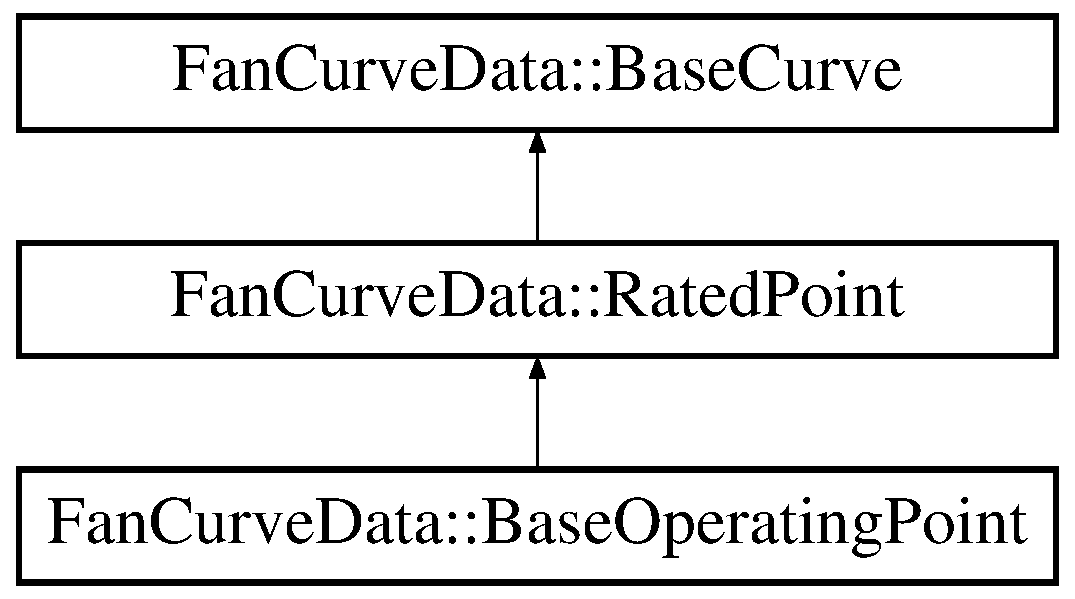
\includegraphics[height=2.533937cm]{d2/da5/struct_fan_curve_data_1_1_rated_point}
\end{center}
\end{figure}
\subsection*{Public Member Functions}
\begin{DoxyCompactItemize}
\item 
\mbox{\Hypertarget{struct_fan_curve_data_1_1_rated_point_a023280b292b8e407d81c433848189f05}\label{struct_fan_curve_data_1_1_rated_point_a023280b292b8e407d81c433848189f05}} 
{\bfseries Rated\+Point} (const double flow, const double pressure, const double power, const double density, const double speed, const double speed\+Corrected)
\item 
\mbox{\Hypertarget{struct_fan_curve_data_1_1_rated_point_a023280b292b8e407d81c433848189f05}\label{struct_fan_curve_data_1_1_rated_point_a023280b292b8e407d81c433848189f05}} 
{\bfseries Rated\+Point} (const double flow, const double pressure, const double power, const double density, const double speed, const double speed\+Corrected)
\item 
\mbox{\Hypertarget{struct_fan_curve_data_1_1_rated_point_a023280b292b8e407d81c433848189f05}\label{struct_fan_curve_data_1_1_rated_point_a023280b292b8e407d81c433848189f05}} 
{\bfseries Rated\+Point} (const double flow, const double pressure, const double power, const double density, const double speed, const double speed\+Corrected)
\end{DoxyCompactItemize}
\subsection*{Public Attributes}
\begin{DoxyCompactItemize}
\item 
\mbox{\Hypertarget{struct_fan_curve_data_1_1_rated_point_ae85a258074490d9691d6ebac53c38b81}\label{struct_fan_curve_data_1_1_rated_point_ae85a258074490d9691d6ebac53c38b81}} 
const double {\bfseries density}
\item 
\mbox{\Hypertarget{struct_fan_curve_data_1_1_rated_point_a48f6364f9e14b8a204fef020f967254e}\label{struct_fan_curve_data_1_1_rated_point_a48f6364f9e14b8a204fef020f967254e}} 
const double {\bfseries speed}
\item 
\mbox{\Hypertarget{struct_fan_curve_data_1_1_rated_point_a845b68ddecfbdbf42c9ea6f0df607a03}\label{struct_fan_curve_data_1_1_rated_point_a845b68ddecfbdbf42c9ea6f0df607a03}} 
const double {\bfseries speed\+Corrected}
\end{DoxyCompactItemize}
\subsection*{Friends}
\begin{DoxyCompactItemize}
\item 
\mbox{\Hypertarget{struct_fan_curve_data_1_1_rated_point_a6c0df668730aa3a6673d279f2bbe7799}\label{struct_fan_curve_data_1_1_rated_point_a6c0df668730aa3a6673d279f2bbe7799}} 
class {\bfseries Fan\+Curve\+Data}
\end{DoxyCompactItemize}


\subsection{Detailed Description}


Definition at line 66 of file Fan\+Curve.\+h.



The documentation for this struct was generated from the following file\+:\begin{DoxyCompactItemize}
\item 
\+\_\+\+C\+Pack\+\_\+\+Packages/\+Darwin/\+S\+T\+G\+Z/amo\+\_\+tools\+\_\+suite-\/-\/\+Darwin-\/x86\+\_\+64/amo\+\_\+tools\+\_\+suite/include/fans/\hyperlink{___c_pack___packages_2_darwin_2_s_t_g_z_2amo__tools__suite--_darwin-x86__64_2amo__tools__suite_2include_2fans_2_fan_curve_8h}{Fan\+Curve.\+h}\end{DoxyCompactItemize}

\hypertarget{class_receiver_tank}{}\section{Receiver\+Tank Class Reference}
\label{class_receiver_tank}\index{Receiver\+Tank@{Receiver\+Tank}}
\subsection*{Public Types}
\begin{DoxyCompactItemize}
\item 
\mbox{\Hypertarget{class_receiver_tank_a8abbc7bc7f04ab853e1334c8905e5832}\label{class_receiver_tank_a8abbc7bc7f04ab853e1334c8905e5832}} 
enum {\bfseries Method} \{ {\bfseries General}, 
{\bfseries Dedicated\+Storage}, 
{\bfseries Metered\+Storage}, 
{\bfseries Bridging\+Compressor\+Reaction\+Delay}
 \}
\end{DoxyCompactItemize}
\subsection*{Public Member Functions}
\begin{DoxyCompactItemize}
\item 
\hyperlink{class_receiver_tank_ad41df65fb570224e135eae7b16c15b81}{Receiver\+Tank} (Method method, double air\+Demand, double allowable\+Pressure\+Drop, double atmospheric\+Pressure)
\item 
\hyperlink{class_receiver_tank_a499e102ca118bfe3bdff3584310207c2}{Receiver\+Tank} (Method method, double length\+Of\+Demand\+Or\+Distance\+To\+Compressor\+Room, double air\+Flow\+Requirement\+Or\+Speed\+Of\+Air, double atmospheric\+Pressure, double initial\+Tank\+Pressure\+Or\+Air\+Demand, double final\+Tank\+Pressure\+Or\+Allowable\+Pressure\+Drop)
\item 
\hyperlink{class_receiver_tank_aba0ca17714d1009c79d6dfcfaa3cea6a}{Receiver\+Tank} (Method method, double length\+Of\+Demand, double air\+Flow\+Requirement, double atmospheric\+Pressure, double initial\+Tank\+Pressure, double final\+Tank\+Pressure, double metered\+Flow\+Control)
\item 
double \hyperlink{class_receiver_tank_a5841344b63c444e4ceb9c3b7daeaf613}{calculate\+Size} ()
\end{DoxyCompactItemize}
\subsection*{Static Public Member Functions}
\begin{DoxyCompactItemize}
\item 
static double \hyperlink{class_receiver_tank_acf0ee7d8a77b01d8c39105c22fbba342}{calculate\+Usable\+Capacity} (double tank\+Size, double air\+Pressure\+In, double air\+Pressure\+Out)
\end{DoxyCompactItemize}


\subsection{Detailed Description}


Definition at line 82 of file Compressed\+Air.\+h.



\subsection{Constructor \& Destructor Documentation}
\mbox{\Hypertarget{class_receiver_tank_ad41df65fb570224e135eae7b16c15b81}\label{class_receiver_tank_ad41df65fb570224e135eae7b16c15b81}} 
\index{Receiver\+Tank@{Receiver\+Tank}!Receiver\+Tank@{Receiver\+Tank}}
\index{Receiver\+Tank@{Receiver\+Tank}!Receiver\+Tank@{Receiver\+Tank}}
\subsubsection{\texorpdfstring{Receiver\+Tank()}{ReceiverTank()}\hspace{0.1cm}{\footnotesize\ttfamily [1/3]}}
{\footnotesize\ttfamily Receiver\+Tank\+::\+Receiver\+Tank (\begin{DoxyParamCaption}\item[{Method}]{method,  }\item[{double}]{air\+Demand,  }\item[{double}]{allowable\+Pressure\+Drop,  }\item[{double}]{atmospheric\+Pressure }\end{DoxyParamCaption})}

Constructor for \hyperlink{class_receiver_tank}{Receiver\+Tank} -\/ This is required when we need to order a receiver tank to meet our compressed air requirements. This calculator computes the quantity of compressed air that is actually available for use. When air receivers are installed, the system’s pressure profile and lack of storage limit the effectiveness of compressed air energy storage. Hence this calculator proves useful in such a context. 
\begin{DoxyParams}{Parameters}
{\em method} & Receiver\+Tank\+::\+Method, Calculation Method, in this case it must be General \\
\hline
{\em air\+Demand} & const double, Amount of air needed, which comes out of the receiver tank -\/ cubic ft \\
\hline
{\em allowable\+Pressure\+Drop} & const double, This decides the pressure drop inside the receiver tank that we can tolerate -\/ psi \\
\hline
{\em atmospheric\+Pressure} & const double, This is generally 14.\+7 psi. In case the receiver tank is at higher altitude location, the respective atmospheric pressure at that location can be given -\/ psi \\
\hline
\end{DoxyParams}


Definition at line 43 of file Compressed\+Air.\+cpp.

\mbox{\Hypertarget{class_receiver_tank_a499e102ca118bfe3bdff3584310207c2}\label{class_receiver_tank_a499e102ca118bfe3bdff3584310207c2}} 
\index{Receiver\+Tank@{Receiver\+Tank}!Receiver\+Tank@{Receiver\+Tank}}
\index{Receiver\+Tank@{Receiver\+Tank}!Receiver\+Tank@{Receiver\+Tank}}
\subsubsection{\texorpdfstring{Receiver\+Tank()}{ReceiverTank()}\hspace{0.1cm}{\footnotesize\ttfamily [2/3]}}
{\footnotesize\ttfamily Receiver\+Tank\+::\+Receiver\+Tank (\begin{DoxyParamCaption}\item[{Method}]{method,  }\item[{double}]{length\+Of\+Demand\+Or\+Distance\+To\+Compressor\+Room,  }\item[{double}]{air\+Flow\+Requirement\+Or\+Speed\+Of\+Air,  }\item[{double}]{atmospheric\+Pressure,  }\item[{double}]{initial\+Tank\+Pressure\+Or\+Air\+Demand,  }\item[{double}]{final\+Tank\+Pressure\+Or\+Allowable\+Pressure\+Drop }\end{DoxyParamCaption})}

Constructor for \hyperlink{class_receiver_tank}{Receiver\+Tank} -\/ This is required when we need to order a receiver tank to meet our compressed air requirements. This calculator computes the quantity of compressed air that is actually available for use. When air receivers are installed, the system’s pressure profile and lack of storage limit the effectiveness of compressed air energy storage. Hence this calculator proves useful in such a context. 
\begin{DoxyParams}{Parameters}
{\em method} & Receiver\+Tank\+::\+Method, Calculation Method, in this case it must be Dedicated\+Storage\+Method OR Bridging\+Compressor\+Reaction\+Delay due to a C++ overloading limitation \\
\hline
{\em length\+Of\+Demand\+Or\+Distance\+To\+Compressor\+Room} & const double, Time duration for which the compressed air is needed OR Distance of the event, that is removing the air, from the compressor room -\/ minutes OR feet \\
\hline
{\em air\+Flow\+Requirement\+Or\+Speed\+Of\+Air} & const double, The quantity of air needed OR Flow rate of air from the tank -\/ cfm OR ft/sec \\
\hline
{\em atmospheric\+Pressure} & const double, This is generally 14.\+7 psi. In case the receiver tank is at higher altitude location, the respective atmospheric pressure at that location can be given -\/ psi \\
\hline
{\em initial\+Tank\+Pressure\+Or\+Air\+Demand} & const double, Tank pressure before release of air OR Amount of air needed, which comes out of the receiver tank -\/ psi OR cubic ft \\
\hline
{\em final\+Tank\+Pressure\+Or\+Allowable\+Pressure\+Drop} & const double, Tank pressure after release of air OR This decides the pressure drop inside the receiver tank that we can tolerate -\/ psi \\
\hline
\end{DoxyParams}


Definition at line 53 of file Compressed\+Air.\+cpp.

\mbox{\Hypertarget{class_receiver_tank_aba0ca17714d1009c79d6dfcfaa3cea6a}\label{class_receiver_tank_aba0ca17714d1009c79d6dfcfaa3cea6a}} 
\index{Receiver\+Tank@{Receiver\+Tank}!Receiver\+Tank@{Receiver\+Tank}}
\index{Receiver\+Tank@{Receiver\+Tank}!Receiver\+Tank@{Receiver\+Tank}}
\subsubsection{\texorpdfstring{Receiver\+Tank()}{ReceiverTank()}\hspace{0.1cm}{\footnotesize\ttfamily [3/3]}}
{\footnotesize\ttfamily Receiver\+Tank\+::\+Receiver\+Tank (\begin{DoxyParamCaption}\item[{Method}]{method,  }\item[{double}]{length\+Of\+Demand,  }\item[{double}]{air\+Flow\+Requirement,  }\item[{double}]{atmospheric\+Pressure,  }\item[{double}]{initial\+Tank\+Pressure,  }\item[{double}]{final\+Tank\+Pressure,  }\item[{double}]{metered\+Flow\+Control }\end{DoxyParamCaption})}

Constructor for \hyperlink{class_receiver_tank}{Receiver\+Tank} -\/ This is required when we need to order a receiver tank to meet our compressed air requirements. This calculator computes the quantity of compressed air that is actually available for use. When air receivers are installed, the system’s pressure profile and lack of storage limit the effectiveness of compressed air energy storage. Hence this calculator proves useful in such a context. 
\begin{DoxyParams}{Parameters}
{\em method} & Receiver\+Tank\+::\+Method, Calculation Method, in this case it must be Metered\+Storage \\
\hline
{\em length\+Of\+Demand} & const double, Time duration for which the compressed air is needed -\/ minutes \\
\hline
{\em air\+Flow\+Requirement} & const double, The quantity of air needed -\/ cfm \\
\hline
{\em atmospheric\+Pressure} & const double, This is generally 14.\+7 psi. In case the receiver tank is at higher altitude location, the respective atmospheric pressure at that location can be given -\/ psi \\
\hline
{\em initial\+Tank\+Pressure} & const double, Tank pressure before release of air -\/ psi \\
\hline
{\em final\+Tank\+Pressure} & const double, Tank pressure after release of air -\/ psi \\
\hline
{\em metered\+Flow\+Control} & const double, Rate of flow through the metering valve (needle valve) -\/ cfm \\
\hline
\end{DoxyParams}


Definition at line 66 of file Compressed\+Air.\+cpp.



\subsection{Member Function Documentation}
\mbox{\Hypertarget{class_receiver_tank_a5841344b63c444e4ceb9c3b7daeaf613}\label{class_receiver_tank_a5841344b63c444e4ceb9c3b7daeaf613}} 
\index{Receiver\+Tank@{Receiver\+Tank}!calculate\+Size@{calculate\+Size}}
\index{calculate\+Size@{calculate\+Size}!Receiver\+Tank@{Receiver\+Tank}}
\subsubsection{\texorpdfstring{calculate\+Size()}{calculateSize()}}
{\footnotesize\ttfamily double Receiver\+Tank\+::calculate\+Size (\begin{DoxyParamCaption}{ }\end{DoxyParamCaption})}

Calculates and returns receiver tank useable air capacity \begin{DoxyReturn}{Returns}
double, receiver size -\/ gallons 
\end{DoxyReturn}


Definition at line 77 of file Compressed\+Air.\+cpp.

\mbox{\Hypertarget{class_receiver_tank_acf0ee7d8a77b01d8c39105c22fbba342}\label{class_receiver_tank_acf0ee7d8a77b01d8c39105c22fbba342}} 
\index{Receiver\+Tank@{Receiver\+Tank}!calculate\+Usable\+Capacity@{calculate\+Usable\+Capacity}}
\index{calculate\+Usable\+Capacity@{calculate\+Usable\+Capacity}!Receiver\+Tank@{Receiver\+Tank}}
\subsubsection{\texorpdfstring{calculate\+Usable\+Capacity()}{calculateUsableCapacity()}}
{\footnotesize\ttfamily double Receiver\+Tank\+::calculate\+Usable\+Capacity (\begin{DoxyParamCaption}\item[{double}]{tank\+Size,  }\item[{double}]{air\+Pressure\+In,  }\item[{double}]{air\+Pressure\+Out }\end{DoxyParamCaption})\hspace{0.3cm}{\ttfamily [static]}}

Calculates and returns receiver tank useable air capacity 
\begin{DoxyParams}{Parameters}
{\em tank\+Size} & double, Quantity of air it can hold -\/ gallons \\
\hline
{\em air\+Pressure\+In} & double, Pressure of air entering the Tank -\/ psi \\
\hline
{\em air\+Pressure\+Out} & double, a. Pressure of air leaving the Tank -\/ psi \\
\hline
\end{DoxyParams}
\begin{DoxyReturn}{Returns}
double, Useable air storage capacity -\/ scf 
\end{DoxyReturn}


Definition at line 37 of file Compressed\+Air.\+cpp.



The documentation for this class was generated from the following files\+:\begin{DoxyCompactItemize}
\item 
include/calculator/util/Compressed\+Air.\+h\item 
src/calculator/util/Compressed\+Air.\+cpp\end{DoxyCompactItemize}

\hypertarget{struct_p_s_a_t_result_1_1result}{}\section{P\+S\+A\+T\+Result\+:\+:result Struct Reference}
\label{struct_p_s_a_t_result_1_1result}\index{P\+S\+A\+T\+Result\+::result@{P\+S\+A\+T\+Result\+::result}}


{\ttfamily \#include $<$P\+S\+A\+T\+Result.\+h$>$}

\subsection*{Public Attributes}
\begin{DoxyCompactItemize}
\item 
double \hyperlink{struct_p_s_a_t_result_1_1result_ab3658ff7a740a5b846b216e9efab0f6f}{pump\+Efficiency}
\begin{DoxyCompactList}\small\item\em Optimal\+: Optimal pump efficiency is estimated based on the efficiency estimating algorithms contained in Hydraulic Institute Standard HI 1.\+3-\/2000, Centrifugal \hyperlink{class_pump}{Pump} Design and Application. \end{DoxyCompactList}\item 
double \hyperlink{struct_p_s_a_t_result_1_1result_acee4fa628de4b65c6fcd58d22432244a}{motor\+Rated\+Power}
\begin{DoxyCompactList}\small\item\em Optimal\+: This is the nameplate motor rated power for an optimally sized pump. \end{DoxyCompactList}\item 
double \hyperlink{struct_p_s_a_t_result_1_1result_a8050ab06ea7a603ad5e5db66e6456c7f}{motor\+Shaft\+Power}
\begin{DoxyCompactList}\small\item\em Optimal\+: This is the motor shaft power requirements for the optimal pump, based on the specified flow rate, head, and specific gravity values, along with the HI 1.\+3 achievable efficiency algorithms. If a belt drive is specified, associated losses are added to the pump shaft power to determine required motor power. For direct-\/driven pumps, the pump and motor shaft powers are the same. \end{DoxyCompactList}\item 
double \hyperlink{struct_p_s_a_t_result_1_1result_ae0b7e90c8f6e8ba8afc1b85c11fcedff}{pump\+Shaft\+Power}
\begin{DoxyCompactList}\small\item\em Optimal\+: This is the shaft power requirements for the optimal pump, based on the specified flow rate, head, and specific gravity values, along with the HI 1.\+3 achievable efficiency algorithms. \end{DoxyCompactList}\item 
double \hyperlink{struct_p_s_a_t_result_1_1result_a92baef08397dc269c233663deeaf6552}{motor\+Efficiency}
\begin{DoxyCompactList}\small\item\em Optimal\+: This is the estimated efficiency for an energy-\/efficient motor of the size indicated in the optimal motor rated power entry above when operating at the optimal motor shaft power. \end{DoxyCompactList}\item 
double \hyperlink{struct_p_s_a_t_result_1_1result_adf9772ebbf9b68a436fbbf75208027b8}{motor\+Power\+Factor}
\begin{DoxyCompactList}\small\item\em Optimal\+: This is the estimated power factor for an energy-\/efficient motor of the size indicated in the optimal motor rated power entry above when operating at the optimal motor shaft power (also indicated above). \end{DoxyCompactList}\item 
double \hyperlink{struct_p_s_a_t_result_1_1result_a1383694c94d04084421e0bd3f3c72af7}{motor\+Current}
\begin{DoxyCompactList}\small\item\em Optimal\+: This is the estimated current for an energy-\/efficient motor of the size indicated in the optimal motor rated power entry above when operating at the optimal motor shaft power. \end{DoxyCompactList}\item 
double \hyperlink{struct_p_s_a_t_result_1_1result_aa51d5a36cf45d9ac779ae395527a81f8}{motor\+Power}
\begin{DoxyCompactList}\small\item\em Optimal\+: The estimated electric power for an energy-\/efficient motor of the size indicated in the optimal motor rated power entry above when operating at the optimal motor shaft power. \end{DoxyCompactList}\item 
double \hyperlink{struct_p_s_a_t_result_1_1result_a0aeab028f0a7cf0ae1cc968161be4a97}{annual\+Energy}
\begin{DoxyCompactList}\small\item\em Optimal\+: The annual energy consumption for an optimized pump driven by an energy-\/efficient motor, based on the estimated motor power and on the fraction of time the pump is operated indicated by the operating fraction. \end{DoxyCompactList}\item 
double \hyperlink{struct_p_s_a_t_result_1_1result_aedad1595120e8b1140020f895d8275fe}{annual\+Cost}
\begin{DoxyCompactList}\small\item\em Optimal\+: This is the annual energy cost based on the product of the optimal annual energy consumption and the unit operating cost (cents/kwhr) input. \end{DoxyCompactList}\item 
\mbox{\Hypertarget{struct_p_s_a_t_result_1_1result_a95949480ff2b7e6d103a955e3b96968c}\label{struct_p_s_a_t_result_1_1result_a95949480ff2b7e6d103a955e3b96968c}} 
double \hyperlink{struct_p_s_a_t_result_1_1result_a95949480ff2b7e6d103a955e3b96968c}{estimated\+F\+LA}
\begin{DoxyCompactList}\small\item\em Existing\+: The full load amps are either specified (known) or estimated. This field will hold either one. The estimated full load amps are calculated from the motor voltage, hp, and speed. \end{DoxyCompactList}\end{DoxyCompactItemize}


\subsection{Detailed Description}
Result structure captures the same fields for the existing as well as the optimal condition. 

Definition at line 77 of file P\+S\+A\+T\+Result.\+h.



\subsection{Member Data Documentation}
\mbox{\Hypertarget{struct_p_s_a_t_result_1_1result_aedad1595120e8b1140020f895d8275fe}\label{struct_p_s_a_t_result_1_1result_aedad1595120e8b1140020f895d8275fe}} 
\index{P\+S\+A\+T\+Result\+::result@{P\+S\+A\+T\+Result\+::result}!annual\+Cost@{annual\+Cost}}
\index{annual\+Cost@{annual\+Cost}!P\+S\+A\+T\+Result\+::result@{P\+S\+A\+T\+Result\+::result}}
\subsubsection{\texorpdfstring{annual\+Cost}{annualCost}}
{\footnotesize\ttfamily double P\+S\+A\+T\+Result\+::result\+::annual\+Cost}



Optimal\+: This is the annual energy cost based on the product of the optimal annual energy consumption and the unit operating cost (cents/kwhr) input. 

Existing\+: This is the existing annual energy cost based on the product of the existing annual energy consumption and the unit operating cost (cents/kwhr) input. 

Definition at line 96 of file P\+S\+A\+T\+Result.\+h.

\mbox{\Hypertarget{struct_p_s_a_t_result_1_1result_a0aeab028f0a7cf0ae1cc968161be4a97}\label{struct_p_s_a_t_result_1_1result_a0aeab028f0a7cf0ae1cc968161be4a97}} 
\index{P\+S\+A\+T\+Result\+::result@{P\+S\+A\+T\+Result\+::result}!annual\+Energy@{annual\+Energy}}
\index{annual\+Energy@{annual\+Energy}!P\+S\+A\+T\+Result\+::result@{P\+S\+A\+T\+Result\+::result}}
\subsubsection{\texorpdfstring{annual\+Energy}{annualEnergy}}
{\footnotesize\ttfamily double P\+S\+A\+T\+Result\+::result\+::annual\+Energy}



Optimal\+: The annual energy consumption for an optimized pump driven by an energy-\/efficient motor, based on the estimated motor power and on the fraction of time the pump is operated indicated by the operating fraction. 

Existing\+: This is the annual energy consumption at the measured/estimated power level for the existing equipment when operated for the fraction of time indicated by the operating fraction. 

Definition at line 94 of file P\+S\+A\+T\+Result.\+h.

\mbox{\Hypertarget{struct_p_s_a_t_result_1_1result_a1383694c94d04084421e0bd3f3c72af7}\label{struct_p_s_a_t_result_1_1result_a1383694c94d04084421e0bd3f3c72af7}} 
\index{P\+S\+A\+T\+Result\+::result@{P\+S\+A\+T\+Result\+::result}!motor\+Current@{motor\+Current}}
\index{motor\+Current@{motor\+Current}!P\+S\+A\+T\+Result\+::result@{P\+S\+A\+T\+Result\+::result}}
\subsubsection{\texorpdfstring{motor\+Current}{motorCurrent}}
{\footnotesize\ttfamily double P\+S\+A\+T\+Result\+::result\+::motor\+Current}



Optimal\+: This is the estimated current for an energy-\/efficient motor of the size indicated in the optimal motor rated power entry above when operating at the optimal motor shaft power. 

Existing\+: This is the estimated or measured current for the existing motor at the existing load. 

Definition at line 90 of file P\+S\+A\+T\+Result.\+h.

\mbox{\Hypertarget{struct_p_s_a_t_result_1_1result_a92baef08397dc269c233663deeaf6552}\label{struct_p_s_a_t_result_1_1result_a92baef08397dc269c233663deeaf6552}} 
\index{P\+S\+A\+T\+Result\+::result@{P\+S\+A\+T\+Result\+::result}!motor\+Efficiency@{motor\+Efficiency}}
\index{motor\+Efficiency@{motor\+Efficiency}!P\+S\+A\+T\+Result\+::result@{P\+S\+A\+T\+Result\+::result}}
\subsubsection{\texorpdfstring{motor\+Efficiency}{motorEfficiency}}
{\footnotesize\ttfamily double P\+S\+A\+T\+Result\+::result\+::motor\+Efficiency}



Optimal\+: This is the estimated efficiency for an energy-\/efficient motor of the size indicated in the optimal motor rated power entry above when operating at the optimal motor shaft power. 

Existing\+: This is the estimated efficiency of the existing motor at the existing load. 

Definition at line 86 of file P\+S\+A\+T\+Result.\+h.

\mbox{\Hypertarget{struct_p_s_a_t_result_1_1result_aa51d5a36cf45d9ac779ae395527a81f8}\label{struct_p_s_a_t_result_1_1result_aa51d5a36cf45d9ac779ae395527a81f8}} 
\index{P\+S\+A\+T\+Result\+::result@{P\+S\+A\+T\+Result\+::result}!motor\+Power@{motor\+Power}}
\index{motor\+Power@{motor\+Power}!P\+S\+A\+T\+Result\+::result@{P\+S\+A\+T\+Result\+::result}}
\subsubsection{\texorpdfstring{motor\+Power}{motorPower}}
{\footnotesize\ttfamily double P\+S\+A\+T\+Result\+::result\+::motor\+Power}



Optimal\+: The estimated electric power for an energy-\/efficient motor of the size indicated in the optimal motor rated power entry above when operating at the optimal motor shaft power. 

Existing\+: This is the estimated or measured electric power for the existing motor at the existing load. 

Definition at line 92 of file P\+S\+A\+T\+Result.\+h.

\mbox{\Hypertarget{struct_p_s_a_t_result_1_1result_adf9772ebbf9b68a436fbbf75208027b8}\label{struct_p_s_a_t_result_1_1result_adf9772ebbf9b68a436fbbf75208027b8}} 
\index{P\+S\+A\+T\+Result\+::result@{P\+S\+A\+T\+Result\+::result}!motor\+Power\+Factor@{motor\+Power\+Factor}}
\index{motor\+Power\+Factor@{motor\+Power\+Factor}!P\+S\+A\+T\+Result\+::result@{P\+S\+A\+T\+Result\+::result}}
\subsubsection{\texorpdfstring{motor\+Power\+Factor}{motorPowerFactor}}
{\footnotesize\ttfamily double P\+S\+A\+T\+Result\+::result\+::motor\+Power\+Factor}



Optimal\+: This is the estimated power factor for an energy-\/efficient motor of the size indicated in the optimal motor rated power entry above when operating at the optimal motor shaft power (also indicated above). 

Existing\+: This is the estimated power factor for the existing motor at the existing load. It is based on the measured electrical data and the motor performance characteristic curves for the specified motor. 

Definition at line 88 of file P\+S\+A\+T\+Result.\+h.

\mbox{\Hypertarget{struct_p_s_a_t_result_1_1result_acee4fa628de4b65c6fcd58d22432244a}\label{struct_p_s_a_t_result_1_1result_acee4fa628de4b65c6fcd58d22432244a}} 
\index{P\+S\+A\+T\+Result\+::result@{P\+S\+A\+T\+Result\+::result}!motor\+Rated\+Power@{motor\+Rated\+Power}}
\index{motor\+Rated\+Power@{motor\+Rated\+Power}!P\+S\+A\+T\+Result\+::result@{P\+S\+A\+T\+Result\+::result}}
\subsubsection{\texorpdfstring{motor\+Rated\+Power}{motorRatedPower}}
{\footnotesize\ttfamily double P\+S\+A\+T\+Result\+::result\+::motor\+Rated\+Power}



Optimal\+: This is the nameplate motor rated power for an optimally sized pump. 

Existing\+: Existing motor nameplate power (same as Rated power in the \hyperlink{class_motor}{Motor} input section). 

Definition at line 80 of file P\+S\+A\+T\+Result.\+h.

\mbox{\Hypertarget{struct_p_s_a_t_result_1_1result_a8050ab06ea7a603ad5e5db66e6456c7f}\label{struct_p_s_a_t_result_1_1result_a8050ab06ea7a603ad5e5db66e6456c7f}} 
\index{P\+S\+A\+T\+Result\+::result@{P\+S\+A\+T\+Result\+::result}!motor\+Shaft\+Power@{motor\+Shaft\+Power}}
\index{motor\+Shaft\+Power@{motor\+Shaft\+Power}!P\+S\+A\+T\+Result\+::result@{P\+S\+A\+T\+Result\+::result}}
\subsubsection{\texorpdfstring{motor\+Shaft\+Power}{motorShaftPower}}
{\footnotesize\ttfamily double P\+S\+A\+T\+Result\+::result\+::motor\+Shaft\+Power}



Optimal\+: This is the motor shaft power requirements for the optimal pump, based on the specified flow rate, head, and specific gravity values, along with the HI 1.\+3 achievable efficiency algorithms. If a belt drive is specified, associated losses are added to the pump shaft power to determine required motor power. For direct-\/driven pumps, the pump and motor shaft powers are the same. 

Existing\+: This is the estimated motor shaft power for the existing motor. The estimate is based on measured electrical data and P\+S\+AT\textquotesingle{}s efficiency estimate for the specified motor size, speed, and class. 

Definition at line 82 of file P\+S\+A\+T\+Result.\+h.

\mbox{\Hypertarget{struct_p_s_a_t_result_1_1result_ab3658ff7a740a5b846b216e9efab0f6f}\label{struct_p_s_a_t_result_1_1result_ab3658ff7a740a5b846b216e9efab0f6f}} 
\index{P\+S\+A\+T\+Result\+::result@{P\+S\+A\+T\+Result\+::result}!pump\+Efficiency@{pump\+Efficiency}}
\index{pump\+Efficiency@{pump\+Efficiency}!P\+S\+A\+T\+Result\+::result@{P\+S\+A\+T\+Result\+::result}}
\subsubsection{\texorpdfstring{pump\+Efficiency}{pumpEfficiency}}
{\footnotesize\ttfamily double P\+S\+A\+T\+Result\+::result\+::pump\+Efficiency}



Optimal\+: Optimal pump efficiency is estimated based on the efficiency estimating algorithms contained in Hydraulic Institute Standard HI 1.\+3-\/2000, Centrifugal \hyperlink{class_pump}{Pump} Design and Application. 

Existing\+: Existing pump efficiency is fluid power added by the pump divided by pump input shaft power. 

Definition at line 78 of file P\+S\+A\+T\+Result.\+h.

\mbox{\Hypertarget{struct_p_s_a_t_result_1_1result_ae0b7e90c8f6e8ba8afc1b85c11fcedff}\label{struct_p_s_a_t_result_1_1result_ae0b7e90c8f6e8ba8afc1b85c11fcedff}} 
\index{P\+S\+A\+T\+Result\+::result@{P\+S\+A\+T\+Result\+::result}!pump\+Shaft\+Power@{pump\+Shaft\+Power}}
\index{pump\+Shaft\+Power@{pump\+Shaft\+Power}!P\+S\+A\+T\+Result\+::result@{P\+S\+A\+T\+Result\+::result}}
\subsubsection{\texorpdfstring{pump\+Shaft\+Power}{pumpShaftPower}}
{\footnotesize\ttfamily double P\+S\+A\+T\+Result\+::result\+::pump\+Shaft\+Power}



Optimal\+: This is the shaft power requirements for the optimal pump, based on the specified flow rate, head, and specific gravity values, along with the HI 1.\+3 achievable efficiency algorithms. 

Existing\+: This is the estimated pump shaft power for the existing motor. The estimate is the same as the motor shaft power (above) for direct-\/driven applications. For belt-\/driven applications, belt losses are deducted from the motor shaft power to determine pump shaft power. 

Definition at line 84 of file P\+S\+A\+T\+Result.\+h.



The documentation for this struct was generated from the following file\+:\begin{DoxyCompactItemize}
\item 
include/psat/\hyperlink{_p_s_a_t_result_8h}{P\+S\+A\+T\+Result.\+h}\end{DoxyCompactItemize}

\hypertarget{class_result_data}{}\section{Result\+Data Class Reference}
\label{class_result_data}\index{Result\+Data@{Result\+Data}}


{\ttfamily \#include $<$Fan\+Curve.\+h$>$}

\subsection*{Public Member Functions}
\begin{DoxyCompactItemize}
\item 
\mbox{\Hypertarget{class_result_data_ab10ba8e317d8b9d830c5f90debfbb15b}\label{class_result_data_ab10ba8e317d8b9d830c5f90debfbb15b}} 
{\bfseries Result\+Data} (const double flow, const double pressure, const double power, const double efficiency)
\item 
\mbox{\Hypertarget{class_result_data_ab10ba8e317d8b9d830c5f90debfbb15b}\label{class_result_data_ab10ba8e317d8b9d830c5f90debfbb15b}} 
{\bfseries Result\+Data} (const double flow, const double pressure, const double power, const double efficiency)
\item 
\mbox{\Hypertarget{class_result_data_ab10ba8e317d8b9d830c5f90debfbb15b}\label{class_result_data_ab10ba8e317d8b9d830c5f90debfbb15b}} 
{\bfseries Result\+Data} (const double flow, const double pressure, const double power, const double efficiency)
\end{DoxyCompactItemize}
\subsection*{Public Attributes}
\begin{DoxyCompactItemize}
\item 
\mbox{\Hypertarget{class_result_data_ae8459ee960a807938dfe6eaa265531cc}\label{class_result_data_ae8459ee960a807938dfe6eaa265531cc}} 
const double {\bfseries flow}
\item 
\mbox{\Hypertarget{class_result_data_a496cd3f0c80f254fcf2ebd7f3476e6dd}\label{class_result_data_a496cd3f0c80f254fcf2ebd7f3476e6dd}} 
const double {\bfseries pressure}
\item 
\mbox{\Hypertarget{class_result_data_a990344826f779c300db9e3128f160c1e}\label{class_result_data_a990344826f779c300db9e3128f160c1e}} 
const double {\bfseries power}
\item 
\mbox{\Hypertarget{class_result_data_a1b75ddc30c8470877bc93bfa6ccafa0e}\label{class_result_data_a1b75ddc30c8470877bc93bfa6ccafa0e}} 
const double {\bfseries efficiency}
\end{DoxyCompactItemize}


\subsection{Detailed Description}
Result Data Calculator class Calculates the result data 

Definition at line 25 of file Fan\+Curve.\+h.



The documentation for this class was generated from the following file\+:\begin{DoxyCompactItemize}
\item 
\+\_\+\+C\+Pack\+\_\+\+Packages/\+Darwin/\+S\+T\+G\+Z/amo\+\_\+tools\+\_\+suite-\/-\/\+Darwin-\/x86\+\_\+64/amo\+\_\+tools\+\_\+suite/include/fans/\hyperlink{___c_pack___packages_2_darwin_2_s_t_g_z_2amo__tools__suite--_darwin-x86__64_2amo__tools__suite_2include_2fans_2_fan_curve_8h}{Fan\+Curve.\+h}\end{DoxyCompactItemize}

\hypertarget{class_saturated_pressure}{}\section{Saturated\+Pressure Class Reference}
\label{class_saturated_pressure}\index{Saturated\+Pressure@{Saturated\+Pressure}}


{\ttfamily \#include $<$Saturated\+Properties.\+h$>$}

\subsection*{Public Member Functions}
\begin{DoxyCompactItemize}
\item 
\hyperlink{class_saturated_pressure_a67020b0bb7588c643e12e256fa25e0bc}{Saturated\+Pressure} (double saturated\+Temperature)
\item 
double \hyperlink{class_saturated_pressure_a8ef5357b4f8af1aeaa8dde6ae05b9daa}{calculate} () const
\item 
\hyperlink{class_saturated_pressure_a67020b0bb7588c643e12e256fa25e0bc}{Saturated\+Pressure} (double saturated\+Temperature)
\item 
double \hyperlink{class_saturated_pressure_a8ef5357b4f8af1aeaa8dde6ae05b9daa}{calculate} () const
\item 
\hyperlink{class_saturated_pressure_a67020b0bb7588c643e12e256fa25e0bc}{Saturated\+Pressure} (double saturated\+Temperature)
\item 
double \hyperlink{class_saturated_pressure_a8ef5357b4f8af1aeaa8dde6ae05b9daa}{calculate} () const
\end{DoxyCompactItemize}


\subsection{Detailed Description}
Saturated pressure class Used to calculate the saturated pressure given the saturated temperature. 

Definition at line 44 of file Saturated\+Properties.\+h.



\subsection{Constructor \& Destructor Documentation}
\mbox{\Hypertarget{class_saturated_pressure_a67020b0bb7588c643e12e256fa25e0bc}\label{class_saturated_pressure_a67020b0bb7588c643e12e256fa25e0bc}} 
\index{Saturated\+Pressure@{Saturated\+Pressure}!Saturated\+Pressure@{Saturated\+Pressure}}
\index{Saturated\+Pressure@{Saturated\+Pressure}!Saturated\+Pressure@{Saturated\+Pressure}}
\subsubsection{\texorpdfstring{Saturated\+Pressure()}{SaturatedPressure()}\hspace{0.1cm}{\footnotesize\ttfamily [1/3]}}
{\footnotesize\ttfamily Saturated\+Pressure\+::\+Saturated\+Pressure (\begin{DoxyParamCaption}\item[{double}]{saturated\+Temperature }\end{DoxyParamCaption})\hspace{0.3cm}{\ttfamily [inline]}, {\ttfamily [explicit]}}

Constructor for the saturated pressure calculator 
\begin{DoxyParams}{Parameters}
{\em saturated\+Temperature} & double, saturated temperature in Kelvin \\
\hline
\end{DoxyParams}


Definition at line 50 of file Saturated\+Properties.\+h.

\mbox{\Hypertarget{class_saturated_pressure_a67020b0bb7588c643e12e256fa25e0bc}\label{class_saturated_pressure_a67020b0bb7588c643e12e256fa25e0bc}} 
\index{Saturated\+Pressure@{Saturated\+Pressure}!Saturated\+Pressure@{Saturated\+Pressure}}
\index{Saturated\+Pressure@{Saturated\+Pressure}!Saturated\+Pressure@{Saturated\+Pressure}}
\subsubsection{\texorpdfstring{Saturated\+Pressure()}{SaturatedPressure()}\hspace{0.1cm}{\footnotesize\ttfamily [2/3]}}
{\footnotesize\ttfamily Saturated\+Pressure\+::\+Saturated\+Pressure (\begin{DoxyParamCaption}\item[{double}]{saturated\+Temperature }\end{DoxyParamCaption})\hspace{0.3cm}{\ttfamily [inline]}, {\ttfamily [explicit]}}

Constructor for the saturated pressure calculator 
\begin{DoxyParams}{Parameters}
{\em saturated\+Temperature} & double, saturated temperature in Kelvin \\
\hline
\end{DoxyParams}


Definition at line 50 of file Saturated\+Properties.\+h.

\mbox{\Hypertarget{class_saturated_pressure_a67020b0bb7588c643e12e256fa25e0bc}\label{class_saturated_pressure_a67020b0bb7588c643e12e256fa25e0bc}} 
\index{Saturated\+Pressure@{Saturated\+Pressure}!Saturated\+Pressure@{Saturated\+Pressure}}
\index{Saturated\+Pressure@{Saturated\+Pressure}!Saturated\+Pressure@{Saturated\+Pressure}}
\subsubsection{\texorpdfstring{Saturated\+Pressure()}{SaturatedPressure()}\hspace{0.1cm}{\footnotesize\ttfamily [3/3]}}
{\footnotesize\ttfamily Saturated\+Pressure\+::\+Saturated\+Pressure (\begin{DoxyParamCaption}\item[{double}]{saturated\+Temperature }\end{DoxyParamCaption})\hspace{0.3cm}{\ttfamily [inline]}, {\ttfamily [explicit]}}

Constructor for the saturated pressure calculator 
\begin{DoxyParams}{Parameters}
{\em saturated\+Temperature} & double, saturated temperature in Kelvin \\
\hline
\end{DoxyParams}


Definition at line 50 of file Saturated\+Properties.\+h.



\subsection{Member Function Documentation}
\mbox{\Hypertarget{class_saturated_pressure_a8ef5357b4f8af1aeaa8dde6ae05b9daa}\label{class_saturated_pressure_a8ef5357b4f8af1aeaa8dde6ae05b9daa}} 
\index{Saturated\+Pressure@{Saturated\+Pressure}!calculate@{calculate}}
\index{calculate@{calculate}!Saturated\+Pressure@{Saturated\+Pressure}}
\subsubsection{\texorpdfstring{calculate()}{calculate()}\hspace{0.1cm}{\footnotesize\ttfamily [1/3]}}
{\footnotesize\ttfamily double Saturated\+Pressure\+::calculate (\begin{DoxyParamCaption}{ }\end{DoxyParamCaption}) const}

Calculates the saturated pressure \begin{DoxyReturn}{Returns}
double, saturated pressure in M\+Pa 
\end{DoxyReturn}


Definition at line 28 of file Saturated\+Properties.\+cpp.

\mbox{\Hypertarget{class_saturated_pressure_a8ef5357b4f8af1aeaa8dde6ae05b9daa}\label{class_saturated_pressure_a8ef5357b4f8af1aeaa8dde6ae05b9daa}} 
\index{Saturated\+Pressure@{Saturated\+Pressure}!calculate@{calculate}}
\index{calculate@{calculate}!Saturated\+Pressure@{Saturated\+Pressure}}
\subsubsection{\texorpdfstring{calculate()}{calculate()}\hspace{0.1cm}{\footnotesize\ttfamily [2/3]}}
{\footnotesize\ttfamily double Saturated\+Pressure\+::calculate (\begin{DoxyParamCaption}{ }\end{DoxyParamCaption}) const}

Calculates the saturated pressure \begin{DoxyReturn}{Returns}
double, saturated pressure in M\+Pa 
\end{DoxyReturn}
\mbox{\Hypertarget{class_saturated_pressure_a8ef5357b4f8af1aeaa8dde6ae05b9daa}\label{class_saturated_pressure_a8ef5357b4f8af1aeaa8dde6ae05b9daa}} 
\index{Saturated\+Pressure@{Saturated\+Pressure}!calculate@{calculate}}
\index{calculate@{calculate}!Saturated\+Pressure@{Saturated\+Pressure}}
\subsubsection{\texorpdfstring{calculate()}{calculate()}\hspace{0.1cm}{\footnotesize\ttfamily [3/3]}}
{\footnotesize\ttfamily double Saturated\+Pressure\+::calculate (\begin{DoxyParamCaption}{ }\end{DoxyParamCaption}) const}

Calculates the saturated pressure \begin{DoxyReturn}{Returns}
double, saturated pressure in M\+Pa 
\end{DoxyReturn}


The documentation for this class was generated from the following files\+:\begin{DoxyCompactItemize}
\item 
\+\_\+\+C\+Pack\+\_\+\+Packages/\+Darwin/\+S\+T\+G\+Z/amo\+\_\+tools\+\_\+suite-\/-\/\+Darwin-\/x86\+\_\+64-\/\+Debug/amo\+\_\+tools\+\_\+suite/include/ssmt/\hyperlink{___c_pack___packages_2_darwin_2_s_t_g_z_2amo__tools__suite--_darwin-x86__64-_debug_2amo__tools__a4aa1517d601f9c2b44ebe76c8c6d4f0}{Saturated\+Properties.\+h}\item 
src/ssmt/\hyperlink{_saturated_properties_8cpp}{Saturated\+Properties.\+cpp}\end{DoxyCompactItemize}

\hypertarget{class_saturated_properties}{}\section{Saturated\+Properties Class Reference}
\label{class_saturated_properties}\index{Saturated\+Properties@{Saturated\+Properties}}


{\ttfamily \#include $<$Saturated\+Properties.\+h$>$}

\subsection*{Public Member Functions}
\begin{DoxyCompactItemize}
\item 
\hyperlink{class_saturated_properties_a83cc16d024ff9bd7ac586df9e946a062}{Saturated\+Properties} (double saturated\+Pressure, double saturated\+Temperature)
\item 
\mbox{\Hypertarget{class_saturated_properties_a73d2c8b16846f3f4801f53f2ef977f80}\label{class_saturated_properties_a73d2c8b16846f3f4801f53f2ef977f80}} 
std\+::unordered\+\_\+map$<$ std\+::string, double $>$ {\bfseries calculate} ()
\end{DoxyCompactItemize}


\subsection{Detailed Description}
Saturated properties class Used to calculate the properties of a saturated substance. 

Definition at line 69 of file Saturated\+Properties.\+h.



\subsection{Constructor \& Destructor Documentation}
\mbox{\Hypertarget{class_saturated_properties_a83cc16d024ff9bd7ac586df9e946a062}\label{class_saturated_properties_a83cc16d024ff9bd7ac586df9e946a062}} 
\index{Saturated\+Properties@{Saturated\+Properties}!Saturated\+Properties@{Saturated\+Properties}}
\index{Saturated\+Properties@{Saturated\+Properties}!Saturated\+Properties@{Saturated\+Properties}}
\subsubsection{\texorpdfstring{Saturated\+Properties()}{SaturatedProperties()}}
{\footnotesize\ttfamily Saturated\+Properties\+::\+Saturated\+Properties (\begin{DoxyParamCaption}\item[{double}]{saturated\+Pressure,  }\item[{double}]{saturated\+Temperature }\end{DoxyParamCaption})\hspace{0.3cm}{\ttfamily [inline]}}

Constructor for the saturated properties calculator 
\begin{DoxyParams}{Parameters}
{\em saturated\+Pressure} & double, saturated pressure in M\+Pa \\
\hline
{\em saturated\+Temperature} & double, saturated temperature in Kelvin \\
\hline
\end{DoxyParams}


Definition at line 76 of file Saturated\+Properties.\+h.



The documentation for this class was generated from the following files\+:\begin{DoxyCompactItemize}
\item 
include/ssmt/\hyperlink{_saturated_properties_8h}{Saturated\+Properties.\+h}\item 
src/ssmt/\hyperlink{_saturated_properties_8cpp}{Saturated\+Properties.\+cpp}\end{DoxyCompactItemize}

\hypertarget{class_saturated_temperature}{}\section{Saturated\+Temperature Class Reference}
\label{class_saturated_temperature}\index{Saturated\+Temperature@{Saturated\+Temperature}}


{\ttfamily \#include $<$Saturated\+Properties.\+h$>$}

\subsection*{Public Member Functions}
\begin{DoxyCompactItemize}
\item 
\hyperlink{class_saturated_temperature_ae0a4b1684a756ac8f91d3ebb646d6865}{Saturated\+Temperature} (double saturated\+Pressure)
\item 
double \hyperlink{class_saturated_temperature_a4aa0d2a337289dd36f4e063f1f67aaa5}{calculate} () const
\item 
\hyperlink{class_saturated_temperature_ae0a4b1684a756ac8f91d3ebb646d6865}{Saturated\+Temperature} (double saturated\+Pressure)
\item 
double \hyperlink{class_saturated_temperature_a4aa0d2a337289dd36f4e063f1f67aaa5}{calculate} () const
\item 
\hyperlink{class_saturated_temperature_ae0a4b1684a756ac8f91d3ebb646d6865}{Saturated\+Temperature} (double saturated\+Pressure)
\item 
double \hyperlink{class_saturated_temperature_a4aa0d2a337289dd36f4e063f1f67aaa5}{calculate} () const
\end{DoxyCompactItemize}


\subsection{Detailed Description}
Saturated temperature class Used to calculate the saturated temperature given the saturated pressure. 

Definition at line 22 of file Saturated\+Properties.\+h.



\subsection{Constructor \& Destructor Documentation}
\mbox{\Hypertarget{class_saturated_temperature_ae0a4b1684a756ac8f91d3ebb646d6865}\label{class_saturated_temperature_ae0a4b1684a756ac8f91d3ebb646d6865}} 
\index{Saturated\+Temperature@{Saturated\+Temperature}!Saturated\+Temperature@{Saturated\+Temperature}}
\index{Saturated\+Temperature@{Saturated\+Temperature}!Saturated\+Temperature@{Saturated\+Temperature}}
\subsubsection{\texorpdfstring{Saturated\+Temperature()}{SaturatedTemperature()}\hspace{0.1cm}{\footnotesize\ttfamily [1/3]}}
{\footnotesize\ttfamily Saturated\+Temperature\+::\+Saturated\+Temperature (\begin{DoxyParamCaption}\item[{double}]{saturated\+Pressure }\end{DoxyParamCaption})\hspace{0.3cm}{\ttfamily [inline]}, {\ttfamily [explicit]}}

Constructor for the saturated temperature calculator


\begin{DoxyParams}{Parameters}
{\em saturated\+Pressure} & double, saturated pressure in M\+Pa\\
\hline
\end{DoxyParams}
\begin{DoxyReturn}{Returns}
nothing 
\end{DoxyReturn}


Definition at line 33 of file Saturated\+Properties.\+h.

\mbox{\Hypertarget{class_saturated_temperature_ae0a4b1684a756ac8f91d3ebb646d6865}\label{class_saturated_temperature_ae0a4b1684a756ac8f91d3ebb646d6865}} 
\index{Saturated\+Temperature@{Saturated\+Temperature}!Saturated\+Temperature@{Saturated\+Temperature}}
\index{Saturated\+Temperature@{Saturated\+Temperature}!Saturated\+Temperature@{Saturated\+Temperature}}
\subsubsection{\texorpdfstring{Saturated\+Temperature()}{SaturatedTemperature()}\hspace{0.1cm}{\footnotesize\ttfamily [2/3]}}
{\footnotesize\ttfamily Saturated\+Temperature\+::\+Saturated\+Temperature (\begin{DoxyParamCaption}\item[{double}]{saturated\+Pressure }\end{DoxyParamCaption})\hspace{0.3cm}{\ttfamily [inline]}, {\ttfamily [explicit]}}

Constructor for the saturated temperature calculator


\begin{DoxyParams}{Parameters}
{\em saturated\+Pressure} & double, saturated pressure in M\+Pa\\
\hline
\end{DoxyParams}
\begin{DoxyReturn}{Returns}
nothing 
\end{DoxyReturn}


Definition at line 33 of file Saturated\+Properties.\+h.

\mbox{\Hypertarget{class_saturated_temperature_ae0a4b1684a756ac8f91d3ebb646d6865}\label{class_saturated_temperature_ae0a4b1684a756ac8f91d3ebb646d6865}} 
\index{Saturated\+Temperature@{Saturated\+Temperature}!Saturated\+Temperature@{Saturated\+Temperature}}
\index{Saturated\+Temperature@{Saturated\+Temperature}!Saturated\+Temperature@{Saturated\+Temperature}}
\subsubsection{\texorpdfstring{Saturated\+Temperature()}{SaturatedTemperature()}\hspace{0.1cm}{\footnotesize\ttfamily [3/3]}}
{\footnotesize\ttfamily Saturated\+Temperature\+::\+Saturated\+Temperature (\begin{DoxyParamCaption}\item[{double}]{saturated\+Pressure }\end{DoxyParamCaption})\hspace{0.3cm}{\ttfamily [inline]}, {\ttfamily [explicit]}}

Constructor for the saturated temperature calculator


\begin{DoxyParams}{Parameters}
{\em saturated\+Pressure} & double, saturated pressure in M\+Pa\\
\hline
\end{DoxyParams}
\begin{DoxyReturn}{Returns}
nothing 
\end{DoxyReturn}


Definition at line 33 of file Saturated\+Properties.\+h.



\subsection{Member Function Documentation}
\mbox{\Hypertarget{class_saturated_temperature_a4aa0d2a337289dd36f4e063f1f67aaa5}\label{class_saturated_temperature_a4aa0d2a337289dd36f4e063f1f67aaa5}} 
\index{Saturated\+Temperature@{Saturated\+Temperature}!calculate@{calculate}}
\index{calculate@{calculate}!Saturated\+Temperature@{Saturated\+Temperature}}
\subsubsection{\texorpdfstring{calculate()}{calculate()}\hspace{0.1cm}{\footnotesize\ttfamily [1/3]}}
{\footnotesize\ttfamily double Saturated\+Temperature\+::calculate (\begin{DoxyParamCaption}{ }\end{DoxyParamCaption}) const}

Calculates the saturated temperature

\begin{DoxyReturn}{Returns}
double, saturated temperature in Kelvin 
\end{DoxyReturn}


Definition at line 13 of file Saturated\+Properties.\+cpp.

\mbox{\Hypertarget{class_saturated_temperature_a4aa0d2a337289dd36f4e063f1f67aaa5}\label{class_saturated_temperature_a4aa0d2a337289dd36f4e063f1f67aaa5}} 
\index{Saturated\+Temperature@{Saturated\+Temperature}!calculate@{calculate}}
\index{calculate@{calculate}!Saturated\+Temperature@{Saturated\+Temperature}}
\subsubsection{\texorpdfstring{calculate()}{calculate()}\hspace{0.1cm}{\footnotesize\ttfamily [2/3]}}
{\footnotesize\ttfamily double Saturated\+Temperature\+::calculate (\begin{DoxyParamCaption}{ }\end{DoxyParamCaption}) const}

Calculates the saturated temperature

\begin{DoxyReturn}{Returns}
double, saturated temperature in Kelvin 
\end{DoxyReturn}
\mbox{\Hypertarget{class_saturated_temperature_a4aa0d2a337289dd36f4e063f1f67aaa5}\label{class_saturated_temperature_a4aa0d2a337289dd36f4e063f1f67aaa5}} 
\index{Saturated\+Temperature@{Saturated\+Temperature}!calculate@{calculate}}
\index{calculate@{calculate}!Saturated\+Temperature@{Saturated\+Temperature}}
\subsubsection{\texorpdfstring{calculate()}{calculate()}\hspace{0.1cm}{\footnotesize\ttfamily [3/3]}}
{\footnotesize\ttfamily double Saturated\+Temperature\+::calculate (\begin{DoxyParamCaption}{ }\end{DoxyParamCaption}) const}

Calculates the saturated temperature

\begin{DoxyReturn}{Returns}
double, saturated temperature in Kelvin 
\end{DoxyReturn}


The documentation for this class was generated from the following files\+:\begin{DoxyCompactItemize}
\item 
\+\_\+\+C\+Pack\+\_\+\+Packages/\+Darwin/\+S\+T\+G\+Z/amo\+\_\+tools\+\_\+suite-\/-\/\+Darwin-\/x86\+\_\+64/amo\+\_\+tools\+\_\+suite/include/ssmt/\hyperlink{___c_pack___packages_2_darwin_2_s_t_g_z_2amo__tools__suite--_darwin-x86__64_2amo__tools__suite_2b97ccf799ea6561aa4d6a618c8073459}{Saturated\+Properties.\+h}\item 
src/ssmt/\hyperlink{_saturated_properties_8cpp}{Saturated\+Properties.\+cpp}\end{DoxyCompactItemize}

\hypertarget{class_slag_other_material_losses}{}\section{Slag\+Other\+Material\+Losses Class Reference}
\label{class_slag_other_material_losses}\index{Slag\+Other\+Material\+Losses@{Slag\+Other\+Material\+Losses}}


{\ttfamily \#include $<$Slag\+Other\+Material\+Losses.\+h$>$}

\subsection*{Public Member Functions}
\begin{DoxyCompactItemize}
\item 
\hyperlink{class_slag_other_material_losses_a8b09bf5dd916a6c7df45b5bf2849e6b8}{Slag\+Other\+Material\+Losses} (double weight, double inlet\+Temperature, double outlet\+Temperature, double specific\+Heat, double correction\+Factor)
\item 
double \hyperlink{class_slag_other_material_losses_a9b62b86eb4ec919d70dd8899ef5d3513}{get\+Weight} () const
\item 
void \hyperlink{class_slag_other_material_losses_a230a178f2ead59cd498b620e4bb4910f}{set\+Weight} (double weight)
\item 
double \hyperlink{class_slag_other_material_losses_aebd0f1b7d6c4bf0deb8ce8a86c5a80a7}{get\+Inlet\+Temperature} () const
\item 
void \hyperlink{class_slag_other_material_losses_a47bb0a61de501e3e9b7bd2bf2651eb8c}{set\+Inlet\+Temperature} (double inlet\+Temperature)
\item 
double \hyperlink{class_slag_other_material_losses_a1c48f1a70aaf030451b7e350f3d6cd18}{get\+Outlet\+Temperature} () const
\item 
void \hyperlink{class_slag_other_material_losses_afae6aafff94d02926135fabf20a87070}{set\+Outlet\+Temperature} (double outlet\+Temperature)
\item 
double \hyperlink{class_slag_other_material_losses_a920bbc2da2ba90416e86573830eee2cb}{get\+Correction\+Factor} () const
\item 
void \hyperlink{class_slag_other_material_losses_a2aa985511888327bed6039da79c8958a}{set\+Correction\+Factor} (double correction\+Factor)
\item 
double \hyperlink{class_slag_other_material_losses_aa68e92bdf836a4112c55344f897f2649}{get\+Specific\+Heat} () const
\item 
void \hyperlink{class_slag_other_material_losses_a05488997f264a74afe3229250a286f92}{set\+Specific\+Heat} (double specific\+Heat)
\item 
void \hyperlink{class_slag_other_material_losses_a33d59aed5492ec2912615e93b6ff273e}{set\+Heat\+Loss} (double total\+Heat)
\item 
double \hyperlink{class_slag_other_material_losses_a4c96a826ef6da38f4c27f7efd8b4a7ba}{get\+Heat\+Loss} ()
\item 
\hyperlink{class_slag_other_material_losses_a8b09bf5dd916a6c7df45b5bf2849e6b8}{Slag\+Other\+Material\+Losses} (double weight, double inlet\+Temperature, double outlet\+Temperature, double specific\+Heat, double correction\+Factor)
\item 
double \hyperlink{class_slag_other_material_losses_a9b62b86eb4ec919d70dd8899ef5d3513}{get\+Weight} () const
\item 
void \hyperlink{class_slag_other_material_losses_a230a178f2ead59cd498b620e4bb4910f}{set\+Weight} (double weight)
\item 
double \hyperlink{class_slag_other_material_losses_aebd0f1b7d6c4bf0deb8ce8a86c5a80a7}{get\+Inlet\+Temperature} () const
\item 
void \hyperlink{class_slag_other_material_losses_a47bb0a61de501e3e9b7bd2bf2651eb8c}{set\+Inlet\+Temperature} (double inlet\+Temperature)
\item 
double \hyperlink{class_slag_other_material_losses_a1c48f1a70aaf030451b7e350f3d6cd18}{get\+Outlet\+Temperature} () const
\item 
void \hyperlink{class_slag_other_material_losses_afae6aafff94d02926135fabf20a87070}{set\+Outlet\+Temperature} (double outlet\+Temperature)
\item 
double \hyperlink{class_slag_other_material_losses_a920bbc2da2ba90416e86573830eee2cb}{get\+Correction\+Factor} () const
\item 
void \hyperlink{class_slag_other_material_losses_a2aa985511888327bed6039da79c8958a}{set\+Correction\+Factor} (double correction\+Factor)
\item 
double \hyperlink{class_slag_other_material_losses_aa68e92bdf836a4112c55344f897f2649}{get\+Specific\+Heat} () const
\item 
void \hyperlink{class_slag_other_material_losses_a05488997f264a74afe3229250a286f92}{set\+Specific\+Heat} (double specific\+Heat)
\item 
void \hyperlink{class_slag_other_material_losses_a33d59aed5492ec2912615e93b6ff273e}{set\+Heat\+Loss} (double total\+Heat)
\item 
double \hyperlink{class_slag_other_material_losses_a4c96a826ef6da38f4c27f7efd8b4a7ba}{get\+Heat\+Loss} ()
\item 
\hyperlink{class_slag_other_material_losses_a8b09bf5dd916a6c7df45b5bf2849e6b8}{Slag\+Other\+Material\+Losses} (double weight, double inlet\+Temperature, double outlet\+Temperature, double specific\+Heat, double correction\+Factor)
\item 
double \hyperlink{class_slag_other_material_losses_a9b62b86eb4ec919d70dd8899ef5d3513}{get\+Weight} () const
\item 
void \hyperlink{class_slag_other_material_losses_a230a178f2ead59cd498b620e4bb4910f}{set\+Weight} (double weight)
\item 
double \hyperlink{class_slag_other_material_losses_aebd0f1b7d6c4bf0deb8ce8a86c5a80a7}{get\+Inlet\+Temperature} () const
\item 
void \hyperlink{class_slag_other_material_losses_a47bb0a61de501e3e9b7bd2bf2651eb8c}{set\+Inlet\+Temperature} (double inlet\+Temperature)
\item 
double \hyperlink{class_slag_other_material_losses_a1c48f1a70aaf030451b7e350f3d6cd18}{get\+Outlet\+Temperature} () const
\item 
void \hyperlink{class_slag_other_material_losses_afae6aafff94d02926135fabf20a87070}{set\+Outlet\+Temperature} (double outlet\+Temperature)
\item 
double \hyperlink{class_slag_other_material_losses_a920bbc2da2ba90416e86573830eee2cb}{get\+Correction\+Factor} () const
\item 
void \hyperlink{class_slag_other_material_losses_a2aa985511888327bed6039da79c8958a}{set\+Correction\+Factor} (double correction\+Factor)
\item 
double \hyperlink{class_slag_other_material_losses_aa68e92bdf836a4112c55344f897f2649}{get\+Specific\+Heat} () const
\item 
void \hyperlink{class_slag_other_material_losses_a05488997f264a74afe3229250a286f92}{set\+Specific\+Heat} (double specific\+Heat)
\item 
void \hyperlink{class_slag_other_material_losses_a33d59aed5492ec2912615e93b6ff273e}{set\+Heat\+Loss} (double total\+Heat)
\item 
double \hyperlink{class_slag_other_material_losses_a4c96a826ef6da38f4c27f7efd8b4a7ba}{get\+Heat\+Loss} ()
\end{DoxyCompactItemize}


\subsection{Detailed Description}
Slag Other Material Losses class Contains all of the properties for slag/waste products. Used to calculate the heat loss caused by having to heat up the slag or other combustion byproducts within the furnace.\textquotesingle{} A\+S\+S\+U\+M\+P\+T\+I\+O\+NS\+: Majority of slag is silicon. Specific heat does not change with temperature. W\+A\+R\+N\+I\+N\+GS\+: Glass structures in slag will change output significantly. 

Definition at line 31 of file Slag\+Other\+Material\+Losses.\+h.



\subsection{Constructor \& Destructor Documentation}
\mbox{\Hypertarget{class_slag_other_material_losses_a8b09bf5dd916a6c7df45b5bf2849e6b8}\label{class_slag_other_material_losses_a8b09bf5dd916a6c7df45b5bf2849e6b8}} 
\index{Slag\+Other\+Material\+Losses@{Slag\+Other\+Material\+Losses}!Slag\+Other\+Material\+Losses@{Slag\+Other\+Material\+Losses}}
\index{Slag\+Other\+Material\+Losses@{Slag\+Other\+Material\+Losses}!Slag\+Other\+Material\+Losses@{Slag\+Other\+Material\+Losses}}
\subsubsection{\texorpdfstring{Slag\+Other\+Material\+Losses()}{SlagOtherMaterialLosses()}\hspace{0.1cm}{\footnotesize\ttfamily [1/3]}}
{\footnotesize\ttfamily Slag\+Other\+Material\+Losses\+::\+Slag\+Other\+Material\+Losses (\begin{DoxyParamCaption}\item[{double}]{weight,  }\item[{double}]{inlet\+Temperature,  }\item[{double}]{outlet\+Temperature,  }\item[{double}]{specific\+Heat,  }\item[{double}]{correction\+Factor }\end{DoxyParamCaption})\hspace{0.3cm}{\ttfamily [inline]}}

Constructor for the slag -\/ other material heat loss with all inputs specified 
\begin{DoxyParams}{Parameters}
{\em weight} & double, weight discharged in Lb/cycle \\
\hline
{\em inlet\+Temperature} & double, initial temperature of charged materials in °F \\
\hline
{\em outlet\+Temperature} & double, Outlet/final temperature in °F \\
\hline
{\em specific\+Heat} & double, Specific heat of material at average air temperature in Btu/(lb$\ast$°F) \\
\hline
{\em correction\+Factor} & double, Correction factor -\/ unitless \\
\hline
\end{DoxyParams}


Definition at line 41 of file Slag\+Other\+Material\+Losses.\+h.

\mbox{\Hypertarget{class_slag_other_material_losses_a8b09bf5dd916a6c7df45b5bf2849e6b8}\label{class_slag_other_material_losses_a8b09bf5dd916a6c7df45b5bf2849e6b8}} 
\index{Slag\+Other\+Material\+Losses@{Slag\+Other\+Material\+Losses}!Slag\+Other\+Material\+Losses@{Slag\+Other\+Material\+Losses}}
\index{Slag\+Other\+Material\+Losses@{Slag\+Other\+Material\+Losses}!Slag\+Other\+Material\+Losses@{Slag\+Other\+Material\+Losses}}
\subsubsection{\texorpdfstring{Slag\+Other\+Material\+Losses()}{SlagOtherMaterialLosses()}\hspace{0.1cm}{\footnotesize\ttfamily [2/3]}}
{\footnotesize\ttfamily Slag\+Other\+Material\+Losses\+::\+Slag\+Other\+Material\+Losses (\begin{DoxyParamCaption}\item[{double}]{weight,  }\item[{double}]{inlet\+Temperature,  }\item[{double}]{outlet\+Temperature,  }\item[{double}]{specific\+Heat,  }\item[{double}]{correction\+Factor }\end{DoxyParamCaption})\hspace{0.3cm}{\ttfamily [inline]}}

Constructor for the slag -\/ other material heat loss with all inputs specified 
\begin{DoxyParams}{Parameters}
{\em weight} & double, weight discharged in Lb/cycle \\
\hline
{\em inlet\+Temperature} & double, initial temperature of charged materials in °F \\
\hline
{\em outlet\+Temperature} & double, Outlet/final temperature in °F \\
\hline
{\em specific\+Heat} & double, Specific heat of material at average air temperature in Btu/(lb$\ast$°F) \\
\hline
{\em correction\+Factor} & double, Correction factor -\/ unitless \\
\hline
\end{DoxyParams}


Definition at line 41 of file Slag\+Other\+Material\+Losses.\+h.

\mbox{\Hypertarget{class_slag_other_material_losses_a8b09bf5dd916a6c7df45b5bf2849e6b8}\label{class_slag_other_material_losses_a8b09bf5dd916a6c7df45b5bf2849e6b8}} 
\index{Slag\+Other\+Material\+Losses@{Slag\+Other\+Material\+Losses}!Slag\+Other\+Material\+Losses@{Slag\+Other\+Material\+Losses}}
\index{Slag\+Other\+Material\+Losses@{Slag\+Other\+Material\+Losses}!Slag\+Other\+Material\+Losses@{Slag\+Other\+Material\+Losses}}
\subsubsection{\texorpdfstring{Slag\+Other\+Material\+Losses()}{SlagOtherMaterialLosses()}\hspace{0.1cm}{\footnotesize\ttfamily [3/3]}}
{\footnotesize\ttfamily Slag\+Other\+Material\+Losses\+::\+Slag\+Other\+Material\+Losses (\begin{DoxyParamCaption}\item[{double}]{weight,  }\item[{double}]{inlet\+Temperature,  }\item[{double}]{outlet\+Temperature,  }\item[{double}]{specific\+Heat,  }\item[{double}]{correction\+Factor }\end{DoxyParamCaption})\hspace{0.3cm}{\ttfamily [inline]}}

Constructor for the slag -\/ other material heat loss with all inputs specified 
\begin{DoxyParams}{Parameters}
{\em weight} & double, weight discharged in Lb/cycle \\
\hline
{\em inlet\+Temperature} & double, initial temperature of charged materials in °F \\
\hline
{\em outlet\+Temperature} & double, Outlet/final temperature in °F \\
\hline
{\em specific\+Heat} & double, Specific heat of material at average air temperature in Btu/(lb$\ast$°F) \\
\hline
{\em correction\+Factor} & double, Correction factor -\/ unitless \\
\hline
\end{DoxyParams}


Definition at line 41 of file Slag\+Other\+Material\+Losses.\+h.



\subsection{Member Function Documentation}
\mbox{\Hypertarget{class_slag_other_material_losses_a920bbc2da2ba90416e86573830eee2cb}\label{class_slag_other_material_losses_a920bbc2da2ba90416e86573830eee2cb}} 
\index{Slag\+Other\+Material\+Losses@{Slag\+Other\+Material\+Losses}!get\+Correction\+Factor@{get\+Correction\+Factor}}
\index{get\+Correction\+Factor@{get\+Correction\+Factor}!Slag\+Other\+Material\+Losses@{Slag\+Other\+Material\+Losses}}
\subsubsection{\texorpdfstring{get\+Correction\+Factor()}{getCorrectionFactor()}\hspace{0.1cm}{\footnotesize\ttfamily [1/3]}}
{\footnotesize\ttfamily double Slag\+Other\+Material\+Losses\+::get\+Correction\+Factor (\begin{DoxyParamCaption}{ }\end{DoxyParamCaption}) const\hspace{0.3cm}{\ttfamily [inline]}}

Gets the correction factor \begin{DoxyReturn}{Returns}
double, correction factor -\/ unitless 
\end{DoxyReturn}


Definition at line 110 of file Slag\+Other\+Material\+Losses.\+h.

\mbox{\Hypertarget{class_slag_other_material_losses_a920bbc2da2ba90416e86573830eee2cb}\label{class_slag_other_material_losses_a920bbc2da2ba90416e86573830eee2cb}} 
\index{Slag\+Other\+Material\+Losses@{Slag\+Other\+Material\+Losses}!get\+Correction\+Factor@{get\+Correction\+Factor}}
\index{get\+Correction\+Factor@{get\+Correction\+Factor}!Slag\+Other\+Material\+Losses@{Slag\+Other\+Material\+Losses}}
\subsubsection{\texorpdfstring{get\+Correction\+Factor()}{getCorrectionFactor()}\hspace{0.1cm}{\footnotesize\ttfamily [2/3]}}
{\footnotesize\ttfamily double Slag\+Other\+Material\+Losses\+::get\+Correction\+Factor (\begin{DoxyParamCaption}{ }\end{DoxyParamCaption}) const\hspace{0.3cm}{\ttfamily [inline]}}

Gets the correction factor \begin{DoxyReturn}{Returns}
double, correction factor -\/ unitless 
\end{DoxyReturn}


Definition at line 110 of file Slag\+Other\+Material\+Losses.\+h.

\mbox{\Hypertarget{class_slag_other_material_losses_a920bbc2da2ba90416e86573830eee2cb}\label{class_slag_other_material_losses_a920bbc2da2ba90416e86573830eee2cb}} 
\index{Slag\+Other\+Material\+Losses@{Slag\+Other\+Material\+Losses}!get\+Correction\+Factor@{get\+Correction\+Factor}}
\index{get\+Correction\+Factor@{get\+Correction\+Factor}!Slag\+Other\+Material\+Losses@{Slag\+Other\+Material\+Losses}}
\subsubsection{\texorpdfstring{get\+Correction\+Factor()}{getCorrectionFactor()}\hspace{0.1cm}{\footnotesize\ttfamily [3/3]}}
{\footnotesize\ttfamily double Slag\+Other\+Material\+Losses\+::get\+Correction\+Factor (\begin{DoxyParamCaption}{ }\end{DoxyParamCaption}) const\hspace{0.3cm}{\ttfamily [inline]}}

Gets the correction factor \begin{DoxyReturn}{Returns}
double, correction factor -\/ unitless 
\end{DoxyReturn}


Definition at line 110 of file Slag\+Other\+Material\+Losses.\+h.

\mbox{\Hypertarget{class_slag_other_material_losses_a4c96a826ef6da38f4c27f7efd8b4a7ba}\label{class_slag_other_material_losses_a4c96a826ef6da38f4c27f7efd8b4a7ba}} 
\index{Slag\+Other\+Material\+Losses@{Slag\+Other\+Material\+Losses}!get\+Heat\+Loss@{get\+Heat\+Loss}}
\index{get\+Heat\+Loss@{get\+Heat\+Loss}!Slag\+Other\+Material\+Losses@{Slag\+Other\+Material\+Losses}}
\subsubsection{\texorpdfstring{get\+Heat\+Loss()}{getHeatLoss()}\hspace{0.1cm}{\footnotesize\ttfamily [1/3]}}
{\footnotesize\ttfamily double Slag\+Other\+Material\+Losses\+::get\+Heat\+Loss (\begin{DoxyParamCaption}{ }\end{DoxyParamCaption})}

Gets the heat loss \begin{DoxyReturn}{Returns}
double, heat loss in kwh/cycle 
\end{DoxyReturn}
\mbox{\Hypertarget{class_slag_other_material_losses_a4c96a826ef6da38f4c27f7efd8b4a7ba}\label{class_slag_other_material_losses_a4c96a826ef6da38f4c27f7efd8b4a7ba}} 
\index{Slag\+Other\+Material\+Losses@{Slag\+Other\+Material\+Losses}!get\+Heat\+Loss@{get\+Heat\+Loss}}
\index{get\+Heat\+Loss@{get\+Heat\+Loss}!Slag\+Other\+Material\+Losses@{Slag\+Other\+Material\+Losses}}
\subsubsection{\texorpdfstring{get\+Heat\+Loss()}{getHeatLoss()}\hspace{0.1cm}{\footnotesize\ttfamily [2/3]}}
{\footnotesize\ttfamily double Slag\+Other\+Material\+Losses\+::get\+Heat\+Loss (\begin{DoxyParamCaption}{ }\end{DoxyParamCaption})}

Gets the heat loss \begin{DoxyReturn}{Returns}
double, heat loss in kwh/cycle 
\end{DoxyReturn}
\mbox{\Hypertarget{class_slag_other_material_losses_a4c96a826ef6da38f4c27f7efd8b4a7ba}\label{class_slag_other_material_losses_a4c96a826ef6da38f4c27f7efd8b4a7ba}} 
\index{Slag\+Other\+Material\+Losses@{Slag\+Other\+Material\+Losses}!get\+Heat\+Loss@{get\+Heat\+Loss}}
\index{get\+Heat\+Loss@{get\+Heat\+Loss}!Slag\+Other\+Material\+Losses@{Slag\+Other\+Material\+Losses}}
\subsubsection{\texorpdfstring{get\+Heat\+Loss()}{getHeatLoss()}\hspace{0.1cm}{\footnotesize\ttfamily [3/3]}}
{\footnotesize\ttfamily double Slag\+Other\+Material\+Losses\+::get\+Heat\+Loss (\begin{DoxyParamCaption}{ }\end{DoxyParamCaption})}

Gets the heat loss \begin{DoxyReturn}{Returns}
double, heat loss in kwh/cycle 
\end{DoxyReturn}


Definition at line 3 of file Slag\+Other\+Material\+Losses.\+cpp.

\mbox{\Hypertarget{class_slag_other_material_losses_aebd0f1b7d6c4bf0deb8ce8a86c5a80a7}\label{class_slag_other_material_losses_aebd0f1b7d6c4bf0deb8ce8a86c5a80a7}} 
\index{Slag\+Other\+Material\+Losses@{Slag\+Other\+Material\+Losses}!get\+Inlet\+Temperature@{get\+Inlet\+Temperature}}
\index{get\+Inlet\+Temperature@{get\+Inlet\+Temperature}!Slag\+Other\+Material\+Losses@{Slag\+Other\+Material\+Losses}}
\subsubsection{\texorpdfstring{get\+Inlet\+Temperature()}{getInletTemperature()}\hspace{0.1cm}{\footnotesize\ttfamily [1/3]}}
{\footnotesize\ttfamily double Slag\+Other\+Material\+Losses\+::get\+Inlet\+Temperature (\begin{DoxyParamCaption}{ }\end{DoxyParamCaption}) const\hspace{0.3cm}{\ttfamily [inline]}}

Gets inlet temperature \begin{DoxyReturn}{Returns}
double, inlet temperature in °F 
\end{DoxyReturn}


Definition at line 77 of file Slag\+Other\+Material\+Losses.\+h.

\mbox{\Hypertarget{class_slag_other_material_losses_aebd0f1b7d6c4bf0deb8ce8a86c5a80a7}\label{class_slag_other_material_losses_aebd0f1b7d6c4bf0deb8ce8a86c5a80a7}} 
\index{Slag\+Other\+Material\+Losses@{Slag\+Other\+Material\+Losses}!get\+Inlet\+Temperature@{get\+Inlet\+Temperature}}
\index{get\+Inlet\+Temperature@{get\+Inlet\+Temperature}!Slag\+Other\+Material\+Losses@{Slag\+Other\+Material\+Losses}}
\subsubsection{\texorpdfstring{get\+Inlet\+Temperature()}{getInletTemperature()}\hspace{0.1cm}{\footnotesize\ttfamily [2/3]}}
{\footnotesize\ttfamily double Slag\+Other\+Material\+Losses\+::get\+Inlet\+Temperature (\begin{DoxyParamCaption}{ }\end{DoxyParamCaption}) const\hspace{0.3cm}{\ttfamily [inline]}}

Gets inlet temperature \begin{DoxyReturn}{Returns}
double, inlet temperature in °F 
\end{DoxyReturn}


Definition at line 77 of file Slag\+Other\+Material\+Losses.\+h.

\mbox{\Hypertarget{class_slag_other_material_losses_aebd0f1b7d6c4bf0deb8ce8a86c5a80a7}\label{class_slag_other_material_losses_aebd0f1b7d6c4bf0deb8ce8a86c5a80a7}} 
\index{Slag\+Other\+Material\+Losses@{Slag\+Other\+Material\+Losses}!get\+Inlet\+Temperature@{get\+Inlet\+Temperature}}
\index{get\+Inlet\+Temperature@{get\+Inlet\+Temperature}!Slag\+Other\+Material\+Losses@{Slag\+Other\+Material\+Losses}}
\subsubsection{\texorpdfstring{get\+Inlet\+Temperature()}{getInletTemperature()}\hspace{0.1cm}{\footnotesize\ttfamily [3/3]}}
{\footnotesize\ttfamily double Slag\+Other\+Material\+Losses\+::get\+Inlet\+Temperature (\begin{DoxyParamCaption}{ }\end{DoxyParamCaption}) const\hspace{0.3cm}{\ttfamily [inline]}}

Gets inlet temperature \begin{DoxyReturn}{Returns}
double, inlet temperature in °F 
\end{DoxyReturn}


Definition at line 77 of file Slag\+Other\+Material\+Losses.\+h.

\mbox{\Hypertarget{class_slag_other_material_losses_a1c48f1a70aaf030451b7e350f3d6cd18}\label{class_slag_other_material_losses_a1c48f1a70aaf030451b7e350f3d6cd18}} 
\index{Slag\+Other\+Material\+Losses@{Slag\+Other\+Material\+Losses}!get\+Outlet\+Temperature@{get\+Outlet\+Temperature}}
\index{get\+Outlet\+Temperature@{get\+Outlet\+Temperature}!Slag\+Other\+Material\+Losses@{Slag\+Other\+Material\+Losses}}
\subsubsection{\texorpdfstring{get\+Outlet\+Temperature()}{getOutletTemperature()}\hspace{0.1cm}{\footnotesize\ttfamily [1/3]}}
{\footnotesize\ttfamily double Slag\+Other\+Material\+Losses\+::get\+Outlet\+Temperature (\begin{DoxyParamCaption}{ }\end{DoxyParamCaption}) const\hspace{0.3cm}{\ttfamily [inline]}}

Gets the outlet temperature \begin{DoxyReturn}{Returns}
double, outlet temperature in °F 
\end{DoxyReturn}


Definition at line 93 of file Slag\+Other\+Material\+Losses.\+h.

\mbox{\Hypertarget{class_slag_other_material_losses_a1c48f1a70aaf030451b7e350f3d6cd18}\label{class_slag_other_material_losses_a1c48f1a70aaf030451b7e350f3d6cd18}} 
\index{Slag\+Other\+Material\+Losses@{Slag\+Other\+Material\+Losses}!get\+Outlet\+Temperature@{get\+Outlet\+Temperature}}
\index{get\+Outlet\+Temperature@{get\+Outlet\+Temperature}!Slag\+Other\+Material\+Losses@{Slag\+Other\+Material\+Losses}}
\subsubsection{\texorpdfstring{get\+Outlet\+Temperature()}{getOutletTemperature()}\hspace{0.1cm}{\footnotesize\ttfamily [2/3]}}
{\footnotesize\ttfamily double Slag\+Other\+Material\+Losses\+::get\+Outlet\+Temperature (\begin{DoxyParamCaption}{ }\end{DoxyParamCaption}) const\hspace{0.3cm}{\ttfamily [inline]}}

Gets the outlet temperature \begin{DoxyReturn}{Returns}
double, outlet temperature in °F 
\end{DoxyReturn}


Definition at line 93 of file Slag\+Other\+Material\+Losses.\+h.

\mbox{\Hypertarget{class_slag_other_material_losses_a1c48f1a70aaf030451b7e350f3d6cd18}\label{class_slag_other_material_losses_a1c48f1a70aaf030451b7e350f3d6cd18}} 
\index{Slag\+Other\+Material\+Losses@{Slag\+Other\+Material\+Losses}!get\+Outlet\+Temperature@{get\+Outlet\+Temperature}}
\index{get\+Outlet\+Temperature@{get\+Outlet\+Temperature}!Slag\+Other\+Material\+Losses@{Slag\+Other\+Material\+Losses}}
\subsubsection{\texorpdfstring{get\+Outlet\+Temperature()}{getOutletTemperature()}\hspace{0.1cm}{\footnotesize\ttfamily [3/3]}}
{\footnotesize\ttfamily double Slag\+Other\+Material\+Losses\+::get\+Outlet\+Temperature (\begin{DoxyParamCaption}{ }\end{DoxyParamCaption}) const\hspace{0.3cm}{\ttfamily [inline]}}

Gets the outlet temperature \begin{DoxyReturn}{Returns}
double, outlet temperature in °F 
\end{DoxyReturn}


Definition at line 93 of file Slag\+Other\+Material\+Losses.\+h.

\mbox{\Hypertarget{class_slag_other_material_losses_aa68e92bdf836a4112c55344f897f2649}\label{class_slag_other_material_losses_aa68e92bdf836a4112c55344f897f2649}} 
\index{Slag\+Other\+Material\+Losses@{Slag\+Other\+Material\+Losses}!get\+Specific\+Heat@{get\+Specific\+Heat}}
\index{get\+Specific\+Heat@{get\+Specific\+Heat}!Slag\+Other\+Material\+Losses@{Slag\+Other\+Material\+Losses}}
\subsubsection{\texorpdfstring{get\+Specific\+Heat()}{getSpecificHeat()}\hspace{0.1cm}{\footnotesize\ttfamily [1/3]}}
{\footnotesize\ttfamily double Slag\+Other\+Material\+Losses\+::get\+Specific\+Heat (\begin{DoxyParamCaption}{ }\end{DoxyParamCaption}) const\hspace{0.3cm}{\ttfamily [inline]}}

Gets the specific heat of material \begin{DoxyReturn}{Returns}
double, specific heat in btu/(lb$\ast$°F) 
\end{DoxyReturn}


Definition at line 126 of file Slag\+Other\+Material\+Losses.\+h.

\mbox{\Hypertarget{class_slag_other_material_losses_aa68e92bdf836a4112c55344f897f2649}\label{class_slag_other_material_losses_aa68e92bdf836a4112c55344f897f2649}} 
\index{Slag\+Other\+Material\+Losses@{Slag\+Other\+Material\+Losses}!get\+Specific\+Heat@{get\+Specific\+Heat}}
\index{get\+Specific\+Heat@{get\+Specific\+Heat}!Slag\+Other\+Material\+Losses@{Slag\+Other\+Material\+Losses}}
\subsubsection{\texorpdfstring{get\+Specific\+Heat()}{getSpecificHeat()}\hspace{0.1cm}{\footnotesize\ttfamily [2/3]}}
{\footnotesize\ttfamily double Slag\+Other\+Material\+Losses\+::get\+Specific\+Heat (\begin{DoxyParamCaption}{ }\end{DoxyParamCaption}) const\hspace{0.3cm}{\ttfamily [inline]}}

Gets the specific heat of material \begin{DoxyReturn}{Returns}
double, specific heat in btu/(lb$\ast$°F) 
\end{DoxyReturn}


Definition at line 126 of file Slag\+Other\+Material\+Losses.\+h.

\mbox{\Hypertarget{class_slag_other_material_losses_aa68e92bdf836a4112c55344f897f2649}\label{class_slag_other_material_losses_aa68e92bdf836a4112c55344f897f2649}} 
\index{Slag\+Other\+Material\+Losses@{Slag\+Other\+Material\+Losses}!get\+Specific\+Heat@{get\+Specific\+Heat}}
\index{get\+Specific\+Heat@{get\+Specific\+Heat}!Slag\+Other\+Material\+Losses@{Slag\+Other\+Material\+Losses}}
\subsubsection{\texorpdfstring{get\+Specific\+Heat()}{getSpecificHeat()}\hspace{0.1cm}{\footnotesize\ttfamily [3/3]}}
{\footnotesize\ttfamily double Slag\+Other\+Material\+Losses\+::get\+Specific\+Heat (\begin{DoxyParamCaption}{ }\end{DoxyParamCaption}) const\hspace{0.3cm}{\ttfamily [inline]}}

Gets the specific heat of material \begin{DoxyReturn}{Returns}
double, specific heat in btu/(lb$\ast$°F) 
\end{DoxyReturn}


Definition at line 126 of file Slag\+Other\+Material\+Losses.\+h.

\mbox{\Hypertarget{class_slag_other_material_losses_a9b62b86eb4ec919d70dd8899ef5d3513}\label{class_slag_other_material_losses_a9b62b86eb4ec919d70dd8899ef5d3513}} 
\index{Slag\+Other\+Material\+Losses@{Slag\+Other\+Material\+Losses}!get\+Weight@{get\+Weight}}
\index{get\+Weight@{get\+Weight}!Slag\+Other\+Material\+Losses@{Slag\+Other\+Material\+Losses}}
\subsubsection{\texorpdfstring{get\+Weight()}{getWeight()}\hspace{0.1cm}{\footnotesize\ttfamily [1/3]}}
{\footnotesize\ttfamily double Slag\+Other\+Material\+Losses\+::get\+Weight (\begin{DoxyParamCaption}{ }\end{DoxyParamCaption}) const\hspace{0.3cm}{\ttfamily [inline]}}

Gets the weight discharged \begin{DoxyReturn}{Returns}
double, weight discharged in lb/cycle 
\end{DoxyReturn}


Definition at line 61 of file Slag\+Other\+Material\+Losses.\+h.

\mbox{\Hypertarget{class_slag_other_material_losses_a9b62b86eb4ec919d70dd8899ef5d3513}\label{class_slag_other_material_losses_a9b62b86eb4ec919d70dd8899ef5d3513}} 
\index{Slag\+Other\+Material\+Losses@{Slag\+Other\+Material\+Losses}!get\+Weight@{get\+Weight}}
\index{get\+Weight@{get\+Weight}!Slag\+Other\+Material\+Losses@{Slag\+Other\+Material\+Losses}}
\subsubsection{\texorpdfstring{get\+Weight()}{getWeight()}\hspace{0.1cm}{\footnotesize\ttfamily [2/3]}}
{\footnotesize\ttfamily double Slag\+Other\+Material\+Losses\+::get\+Weight (\begin{DoxyParamCaption}{ }\end{DoxyParamCaption}) const\hspace{0.3cm}{\ttfamily [inline]}}

Gets the weight discharged \begin{DoxyReturn}{Returns}
double, weight discharged in lb/cycle 
\end{DoxyReturn}


Definition at line 61 of file Slag\+Other\+Material\+Losses.\+h.

\mbox{\Hypertarget{class_slag_other_material_losses_a9b62b86eb4ec919d70dd8899ef5d3513}\label{class_slag_other_material_losses_a9b62b86eb4ec919d70dd8899ef5d3513}} 
\index{Slag\+Other\+Material\+Losses@{Slag\+Other\+Material\+Losses}!get\+Weight@{get\+Weight}}
\index{get\+Weight@{get\+Weight}!Slag\+Other\+Material\+Losses@{Slag\+Other\+Material\+Losses}}
\subsubsection{\texorpdfstring{get\+Weight()}{getWeight()}\hspace{0.1cm}{\footnotesize\ttfamily [3/3]}}
{\footnotesize\ttfamily double Slag\+Other\+Material\+Losses\+::get\+Weight (\begin{DoxyParamCaption}{ }\end{DoxyParamCaption}) const\hspace{0.3cm}{\ttfamily [inline]}}

Gets the weight discharged \begin{DoxyReturn}{Returns}
double, weight discharged in lb/cycle 
\end{DoxyReturn}


Definition at line 61 of file Slag\+Other\+Material\+Losses.\+h.

\mbox{\Hypertarget{class_slag_other_material_losses_a2aa985511888327bed6039da79c8958a}\label{class_slag_other_material_losses_a2aa985511888327bed6039da79c8958a}} 
\index{Slag\+Other\+Material\+Losses@{Slag\+Other\+Material\+Losses}!set\+Correction\+Factor@{set\+Correction\+Factor}}
\index{set\+Correction\+Factor@{set\+Correction\+Factor}!Slag\+Other\+Material\+Losses@{Slag\+Other\+Material\+Losses}}
\subsubsection{\texorpdfstring{set\+Correction\+Factor()}{setCorrectionFactor()}\hspace{0.1cm}{\footnotesize\ttfamily [1/3]}}
{\footnotesize\ttfamily void Slag\+Other\+Material\+Losses\+::set\+Correction\+Factor (\begin{DoxyParamCaption}\item[{double}]{correction\+Factor }\end{DoxyParamCaption})\hspace{0.3cm}{\ttfamily [inline]}}

Sets correction factor 
\begin{DoxyParams}{Parameters}
{\em correction\+Factor} & double, correction factor -\/ unitless \\
\hline
\end{DoxyParams}


Definition at line 118 of file Slag\+Other\+Material\+Losses.\+h.

\mbox{\Hypertarget{class_slag_other_material_losses_a2aa985511888327bed6039da79c8958a}\label{class_slag_other_material_losses_a2aa985511888327bed6039da79c8958a}} 
\index{Slag\+Other\+Material\+Losses@{Slag\+Other\+Material\+Losses}!set\+Correction\+Factor@{set\+Correction\+Factor}}
\index{set\+Correction\+Factor@{set\+Correction\+Factor}!Slag\+Other\+Material\+Losses@{Slag\+Other\+Material\+Losses}}
\subsubsection{\texorpdfstring{set\+Correction\+Factor()}{setCorrectionFactor()}\hspace{0.1cm}{\footnotesize\ttfamily [2/3]}}
{\footnotesize\ttfamily void Slag\+Other\+Material\+Losses\+::set\+Correction\+Factor (\begin{DoxyParamCaption}\item[{double}]{correction\+Factor }\end{DoxyParamCaption})\hspace{0.3cm}{\ttfamily [inline]}}

Sets correction factor 
\begin{DoxyParams}{Parameters}
{\em correction\+Factor} & double, correction factor -\/ unitless \\
\hline
\end{DoxyParams}


Definition at line 118 of file Slag\+Other\+Material\+Losses.\+h.

\mbox{\Hypertarget{class_slag_other_material_losses_a2aa985511888327bed6039da79c8958a}\label{class_slag_other_material_losses_a2aa985511888327bed6039da79c8958a}} 
\index{Slag\+Other\+Material\+Losses@{Slag\+Other\+Material\+Losses}!set\+Correction\+Factor@{set\+Correction\+Factor}}
\index{set\+Correction\+Factor@{set\+Correction\+Factor}!Slag\+Other\+Material\+Losses@{Slag\+Other\+Material\+Losses}}
\subsubsection{\texorpdfstring{set\+Correction\+Factor()}{setCorrectionFactor()}\hspace{0.1cm}{\footnotesize\ttfamily [3/3]}}
{\footnotesize\ttfamily void Slag\+Other\+Material\+Losses\+::set\+Correction\+Factor (\begin{DoxyParamCaption}\item[{double}]{correction\+Factor }\end{DoxyParamCaption})\hspace{0.3cm}{\ttfamily [inline]}}

Sets correction factor 
\begin{DoxyParams}{Parameters}
{\em correction\+Factor} & double, correction factor -\/ unitless \\
\hline
\end{DoxyParams}


Definition at line 118 of file Slag\+Other\+Material\+Losses.\+h.

\mbox{\Hypertarget{class_slag_other_material_losses_a33d59aed5492ec2912615e93b6ff273e}\label{class_slag_other_material_losses_a33d59aed5492ec2912615e93b6ff273e}} 
\index{Slag\+Other\+Material\+Losses@{Slag\+Other\+Material\+Losses}!set\+Heat\+Loss@{set\+Heat\+Loss}}
\index{set\+Heat\+Loss@{set\+Heat\+Loss}!Slag\+Other\+Material\+Losses@{Slag\+Other\+Material\+Losses}}
\subsubsection{\texorpdfstring{set\+Heat\+Loss()}{setHeatLoss()}\hspace{0.1cm}{\footnotesize\ttfamily [1/3]}}
{\footnotesize\ttfamily void Slag\+Other\+Material\+Losses\+::set\+Heat\+Loss (\begin{DoxyParamCaption}\item[{double}]{total\+Heat }\end{DoxyParamCaption})\hspace{0.3cm}{\ttfamily [inline]}}

Sets the heat loss \begin{DoxyReturn}{Returns}
double, heat loss in kwh/cycle 
\end{DoxyReturn}


Definition at line 142 of file Slag\+Other\+Material\+Losses.\+h.

\mbox{\Hypertarget{class_slag_other_material_losses_a33d59aed5492ec2912615e93b6ff273e}\label{class_slag_other_material_losses_a33d59aed5492ec2912615e93b6ff273e}} 
\index{Slag\+Other\+Material\+Losses@{Slag\+Other\+Material\+Losses}!set\+Heat\+Loss@{set\+Heat\+Loss}}
\index{set\+Heat\+Loss@{set\+Heat\+Loss}!Slag\+Other\+Material\+Losses@{Slag\+Other\+Material\+Losses}}
\subsubsection{\texorpdfstring{set\+Heat\+Loss()}{setHeatLoss()}\hspace{0.1cm}{\footnotesize\ttfamily [2/3]}}
{\footnotesize\ttfamily void Slag\+Other\+Material\+Losses\+::set\+Heat\+Loss (\begin{DoxyParamCaption}\item[{double}]{total\+Heat }\end{DoxyParamCaption})\hspace{0.3cm}{\ttfamily [inline]}}

Sets the heat loss \begin{DoxyReturn}{Returns}
double, heat loss in kwh/cycle 
\end{DoxyReturn}


Definition at line 142 of file Slag\+Other\+Material\+Losses.\+h.

\mbox{\Hypertarget{class_slag_other_material_losses_a33d59aed5492ec2912615e93b6ff273e}\label{class_slag_other_material_losses_a33d59aed5492ec2912615e93b6ff273e}} 
\index{Slag\+Other\+Material\+Losses@{Slag\+Other\+Material\+Losses}!set\+Heat\+Loss@{set\+Heat\+Loss}}
\index{set\+Heat\+Loss@{set\+Heat\+Loss}!Slag\+Other\+Material\+Losses@{Slag\+Other\+Material\+Losses}}
\subsubsection{\texorpdfstring{set\+Heat\+Loss()}{setHeatLoss()}\hspace{0.1cm}{\footnotesize\ttfamily [3/3]}}
{\footnotesize\ttfamily void Slag\+Other\+Material\+Losses\+::set\+Heat\+Loss (\begin{DoxyParamCaption}\item[{double}]{total\+Heat }\end{DoxyParamCaption})\hspace{0.3cm}{\ttfamily [inline]}}

Sets the heat loss \begin{DoxyReturn}{Returns}
double, heat loss in kwh/cycle 
\end{DoxyReturn}


Definition at line 142 of file Slag\+Other\+Material\+Losses.\+h.

\mbox{\Hypertarget{class_slag_other_material_losses_a47bb0a61de501e3e9b7bd2bf2651eb8c}\label{class_slag_other_material_losses_a47bb0a61de501e3e9b7bd2bf2651eb8c}} 
\index{Slag\+Other\+Material\+Losses@{Slag\+Other\+Material\+Losses}!set\+Inlet\+Temperature@{set\+Inlet\+Temperature}}
\index{set\+Inlet\+Temperature@{set\+Inlet\+Temperature}!Slag\+Other\+Material\+Losses@{Slag\+Other\+Material\+Losses}}
\subsubsection{\texorpdfstring{set\+Inlet\+Temperature()}{setInletTemperature()}\hspace{0.1cm}{\footnotesize\ttfamily [1/3]}}
{\footnotesize\ttfamily void Slag\+Other\+Material\+Losses\+::set\+Inlet\+Temperature (\begin{DoxyParamCaption}\item[{double}]{inlet\+Temperature }\end{DoxyParamCaption})\hspace{0.3cm}{\ttfamily [inline]}}

Sets the inlet temperature 
\begin{DoxyParams}{Parameters}
{\em inlet\+Temperature} & double, inlet temperature in °F \\
\hline
\end{DoxyParams}


Definition at line 85 of file Slag\+Other\+Material\+Losses.\+h.

\mbox{\Hypertarget{class_slag_other_material_losses_a47bb0a61de501e3e9b7bd2bf2651eb8c}\label{class_slag_other_material_losses_a47bb0a61de501e3e9b7bd2bf2651eb8c}} 
\index{Slag\+Other\+Material\+Losses@{Slag\+Other\+Material\+Losses}!set\+Inlet\+Temperature@{set\+Inlet\+Temperature}}
\index{set\+Inlet\+Temperature@{set\+Inlet\+Temperature}!Slag\+Other\+Material\+Losses@{Slag\+Other\+Material\+Losses}}
\subsubsection{\texorpdfstring{set\+Inlet\+Temperature()}{setInletTemperature()}\hspace{0.1cm}{\footnotesize\ttfamily [2/3]}}
{\footnotesize\ttfamily void Slag\+Other\+Material\+Losses\+::set\+Inlet\+Temperature (\begin{DoxyParamCaption}\item[{double}]{inlet\+Temperature }\end{DoxyParamCaption})\hspace{0.3cm}{\ttfamily [inline]}}

Sets the inlet temperature 
\begin{DoxyParams}{Parameters}
{\em inlet\+Temperature} & double, inlet temperature in °F \\
\hline
\end{DoxyParams}


Definition at line 85 of file Slag\+Other\+Material\+Losses.\+h.

\mbox{\Hypertarget{class_slag_other_material_losses_a47bb0a61de501e3e9b7bd2bf2651eb8c}\label{class_slag_other_material_losses_a47bb0a61de501e3e9b7bd2bf2651eb8c}} 
\index{Slag\+Other\+Material\+Losses@{Slag\+Other\+Material\+Losses}!set\+Inlet\+Temperature@{set\+Inlet\+Temperature}}
\index{set\+Inlet\+Temperature@{set\+Inlet\+Temperature}!Slag\+Other\+Material\+Losses@{Slag\+Other\+Material\+Losses}}
\subsubsection{\texorpdfstring{set\+Inlet\+Temperature()}{setInletTemperature()}\hspace{0.1cm}{\footnotesize\ttfamily [3/3]}}
{\footnotesize\ttfamily void Slag\+Other\+Material\+Losses\+::set\+Inlet\+Temperature (\begin{DoxyParamCaption}\item[{double}]{inlet\+Temperature }\end{DoxyParamCaption})\hspace{0.3cm}{\ttfamily [inline]}}

Sets the inlet temperature 
\begin{DoxyParams}{Parameters}
{\em inlet\+Temperature} & double, inlet temperature in °F \\
\hline
\end{DoxyParams}


Definition at line 85 of file Slag\+Other\+Material\+Losses.\+h.

\mbox{\Hypertarget{class_slag_other_material_losses_afae6aafff94d02926135fabf20a87070}\label{class_slag_other_material_losses_afae6aafff94d02926135fabf20a87070}} 
\index{Slag\+Other\+Material\+Losses@{Slag\+Other\+Material\+Losses}!set\+Outlet\+Temperature@{set\+Outlet\+Temperature}}
\index{set\+Outlet\+Temperature@{set\+Outlet\+Temperature}!Slag\+Other\+Material\+Losses@{Slag\+Other\+Material\+Losses}}
\subsubsection{\texorpdfstring{set\+Outlet\+Temperature()}{setOutletTemperature()}\hspace{0.1cm}{\footnotesize\ttfamily [1/3]}}
{\footnotesize\ttfamily void Slag\+Other\+Material\+Losses\+::set\+Outlet\+Temperature (\begin{DoxyParamCaption}\item[{double}]{outlet\+Temperature }\end{DoxyParamCaption})\hspace{0.3cm}{\ttfamily [inline]}}

Sets outlet temperature 
\begin{DoxyParams}{Parameters}
{\em outlet\+Temperature} & double, outlet temperature in °F \\
\hline
\end{DoxyParams}


Definition at line 101 of file Slag\+Other\+Material\+Losses.\+h.

\mbox{\Hypertarget{class_slag_other_material_losses_afae6aafff94d02926135fabf20a87070}\label{class_slag_other_material_losses_afae6aafff94d02926135fabf20a87070}} 
\index{Slag\+Other\+Material\+Losses@{Slag\+Other\+Material\+Losses}!set\+Outlet\+Temperature@{set\+Outlet\+Temperature}}
\index{set\+Outlet\+Temperature@{set\+Outlet\+Temperature}!Slag\+Other\+Material\+Losses@{Slag\+Other\+Material\+Losses}}
\subsubsection{\texorpdfstring{set\+Outlet\+Temperature()}{setOutletTemperature()}\hspace{0.1cm}{\footnotesize\ttfamily [2/3]}}
{\footnotesize\ttfamily void Slag\+Other\+Material\+Losses\+::set\+Outlet\+Temperature (\begin{DoxyParamCaption}\item[{double}]{outlet\+Temperature }\end{DoxyParamCaption})\hspace{0.3cm}{\ttfamily [inline]}}

Sets outlet temperature 
\begin{DoxyParams}{Parameters}
{\em outlet\+Temperature} & double, outlet temperature in °F \\
\hline
\end{DoxyParams}


Definition at line 101 of file Slag\+Other\+Material\+Losses.\+h.

\mbox{\Hypertarget{class_slag_other_material_losses_afae6aafff94d02926135fabf20a87070}\label{class_slag_other_material_losses_afae6aafff94d02926135fabf20a87070}} 
\index{Slag\+Other\+Material\+Losses@{Slag\+Other\+Material\+Losses}!set\+Outlet\+Temperature@{set\+Outlet\+Temperature}}
\index{set\+Outlet\+Temperature@{set\+Outlet\+Temperature}!Slag\+Other\+Material\+Losses@{Slag\+Other\+Material\+Losses}}
\subsubsection{\texorpdfstring{set\+Outlet\+Temperature()}{setOutletTemperature()}\hspace{0.1cm}{\footnotesize\ttfamily [3/3]}}
{\footnotesize\ttfamily void Slag\+Other\+Material\+Losses\+::set\+Outlet\+Temperature (\begin{DoxyParamCaption}\item[{double}]{outlet\+Temperature }\end{DoxyParamCaption})\hspace{0.3cm}{\ttfamily [inline]}}

Sets outlet temperature 
\begin{DoxyParams}{Parameters}
{\em outlet\+Temperature} & double, outlet temperature in °F \\
\hline
\end{DoxyParams}


Definition at line 101 of file Slag\+Other\+Material\+Losses.\+h.

\mbox{\Hypertarget{class_slag_other_material_losses_a05488997f264a74afe3229250a286f92}\label{class_slag_other_material_losses_a05488997f264a74afe3229250a286f92}} 
\index{Slag\+Other\+Material\+Losses@{Slag\+Other\+Material\+Losses}!set\+Specific\+Heat@{set\+Specific\+Heat}}
\index{set\+Specific\+Heat@{set\+Specific\+Heat}!Slag\+Other\+Material\+Losses@{Slag\+Other\+Material\+Losses}}
\subsubsection{\texorpdfstring{set\+Specific\+Heat()}{setSpecificHeat()}\hspace{0.1cm}{\footnotesize\ttfamily [1/3]}}
{\footnotesize\ttfamily void Slag\+Other\+Material\+Losses\+::set\+Specific\+Heat (\begin{DoxyParamCaption}\item[{double}]{specific\+Heat }\end{DoxyParamCaption})\hspace{0.3cm}{\ttfamily [inline]}}

Sets the specific heat of material 
\begin{DoxyParams}{Parameters}
{\em specific\+Heat} & double, specific heat of material in btu/(lb$\ast$°F) \\
\hline
\end{DoxyParams}


Definition at line 134 of file Slag\+Other\+Material\+Losses.\+h.

\mbox{\Hypertarget{class_slag_other_material_losses_a05488997f264a74afe3229250a286f92}\label{class_slag_other_material_losses_a05488997f264a74afe3229250a286f92}} 
\index{Slag\+Other\+Material\+Losses@{Slag\+Other\+Material\+Losses}!set\+Specific\+Heat@{set\+Specific\+Heat}}
\index{set\+Specific\+Heat@{set\+Specific\+Heat}!Slag\+Other\+Material\+Losses@{Slag\+Other\+Material\+Losses}}
\subsubsection{\texorpdfstring{set\+Specific\+Heat()}{setSpecificHeat()}\hspace{0.1cm}{\footnotesize\ttfamily [2/3]}}
{\footnotesize\ttfamily void Slag\+Other\+Material\+Losses\+::set\+Specific\+Heat (\begin{DoxyParamCaption}\item[{double}]{specific\+Heat }\end{DoxyParamCaption})\hspace{0.3cm}{\ttfamily [inline]}}

Sets the specific heat of material 
\begin{DoxyParams}{Parameters}
{\em specific\+Heat} & double, specific heat of material in btu/(lb$\ast$°F) \\
\hline
\end{DoxyParams}


Definition at line 134 of file Slag\+Other\+Material\+Losses.\+h.

\mbox{\Hypertarget{class_slag_other_material_losses_a05488997f264a74afe3229250a286f92}\label{class_slag_other_material_losses_a05488997f264a74afe3229250a286f92}} 
\index{Slag\+Other\+Material\+Losses@{Slag\+Other\+Material\+Losses}!set\+Specific\+Heat@{set\+Specific\+Heat}}
\index{set\+Specific\+Heat@{set\+Specific\+Heat}!Slag\+Other\+Material\+Losses@{Slag\+Other\+Material\+Losses}}
\subsubsection{\texorpdfstring{set\+Specific\+Heat()}{setSpecificHeat()}\hspace{0.1cm}{\footnotesize\ttfamily [3/3]}}
{\footnotesize\ttfamily void Slag\+Other\+Material\+Losses\+::set\+Specific\+Heat (\begin{DoxyParamCaption}\item[{double}]{specific\+Heat }\end{DoxyParamCaption})\hspace{0.3cm}{\ttfamily [inline]}}

Sets the specific heat of material 
\begin{DoxyParams}{Parameters}
{\em specific\+Heat} & double, specific heat of material in btu/(lb$\ast$°F) \\
\hline
\end{DoxyParams}


Definition at line 134 of file Slag\+Other\+Material\+Losses.\+h.

\mbox{\Hypertarget{class_slag_other_material_losses_a230a178f2ead59cd498b620e4bb4910f}\label{class_slag_other_material_losses_a230a178f2ead59cd498b620e4bb4910f}} 
\index{Slag\+Other\+Material\+Losses@{Slag\+Other\+Material\+Losses}!set\+Weight@{set\+Weight}}
\index{set\+Weight@{set\+Weight}!Slag\+Other\+Material\+Losses@{Slag\+Other\+Material\+Losses}}
\subsubsection{\texorpdfstring{set\+Weight()}{setWeight()}\hspace{0.1cm}{\footnotesize\ttfamily [1/3]}}
{\footnotesize\ttfamily void Slag\+Other\+Material\+Losses\+::set\+Weight (\begin{DoxyParamCaption}\item[{double}]{weight }\end{DoxyParamCaption})\hspace{0.3cm}{\ttfamily [inline]}}

Sets the weight discharged 
\begin{DoxyParams}{Parameters}
{\em weight} & double, weight discharged in lb/cycle \\
\hline
\end{DoxyParams}


Definition at line 69 of file Slag\+Other\+Material\+Losses.\+h.

\mbox{\Hypertarget{class_slag_other_material_losses_a230a178f2ead59cd498b620e4bb4910f}\label{class_slag_other_material_losses_a230a178f2ead59cd498b620e4bb4910f}} 
\index{Slag\+Other\+Material\+Losses@{Slag\+Other\+Material\+Losses}!set\+Weight@{set\+Weight}}
\index{set\+Weight@{set\+Weight}!Slag\+Other\+Material\+Losses@{Slag\+Other\+Material\+Losses}}
\subsubsection{\texorpdfstring{set\+Weight()}{setWeight()}\hspace{0.1cm}{\footnotesize\ttfamily [2/3]}}
{\footnotesize\ttfamily void Slag\+Other\+Material\+Losses\+::set\+Weight (\begin{DoxyParamCaption}\item[{double}]{weight }\end{DoxyParamCaption})\hspace{0.3cm}{\ttfamily [inline]}}

Sets the weight discharged 
\begin{DoxyParams}{Parameters}
{\em weight} & double, weight discharged in lb/cycle \\
\hline
\end{DoxyParams}


Definition at line 69 of file Slag\+Other\+Material\+Losses.\+h.

\mbox{\Hypertarget{class_slag_other_material_losses_a230a178f2ead59cd498b620e4bb4910f}\label{class_slag_other_material_losses_a230a178f2ead59cd498b620e4bb4910f}} 
\index{Slag\+Other\+Material\+Losses@{Slag\+Other\+Material\+Losses}!set\+Weight@{set\+Weight}}
\index{set\+Weight@{set\+Weight}!Slag\+Other\+Material\+Losses@{Slag\+Other\+Material\+Losses}}
\subsubsection{\texorpdfstring{set\+Weight()}{setWeight()}\hspace{0.1cm}{\footnotesize\ttfamily [3/3]}}
{\footnotesize\ttfamily void Slag\+Other\+Material\+Losses\+::set\+Weight (\begin{DoxyParamCaption}\item[{double}]{weight }\end{DoxyParamCaption})\hspace{0.3cm}{\ttfamily [inline]}}

Sets the weight discharged 
\begin{DoxyParams}{Parameters}
{\em weight} & double, weight discharged in lb/cycle \\
\hline
\end{DoxyParams}


Definition at line 69 of file Slag\+Other\+Material\+Losses.\+h.



The documentation for this class was generated from the following files\+:\begin{DoxyCompactItemize}
\item 
\+\_\+\+C\+Pack\+\_\+\+Packages/\+Darwin/\+S\+T\+G\+Z/amo\+\_\+tools\+\_\+suite-\/-\/\+Darwin-\/x86\+\_\+64-\/\+Debug/amo\+\_\+tools\+\_\+suite/include/calculator/losses/\hyperlink{___c_pack___packages_2_darwin_2_s_t_g_z_2amo__tools__suite--_darwin-x86__64-_debug_2amo__tools__a360f170cb779488bbc84e310d33960e}{Slag\+Other\+Material\+Losses.\+h}\item 
src/calculator/losses/Slag\+Other\+Material\+Losses.\+cpp\end{DoxyCompactItemize}

\hypertarget{class_solid_liquid_flue_gas_material}{}\section{Solid\+Liquid\+Flue\+Gas\+Material Class Reference}
\label{class_solid_liquid_flue_gas_material}\index{Solid\+Liquid\+Flue\+Gas\+Material@{Solid\+Liquid\+Flue\+Gas\+Material}}


{\ttfamily \#include $<$Solid\+Liquid\+Flue\+Gas\+Material.\+h$>$}

\subsection*{Public Member Functions}
\begin{DoxyCompactItemize}
\item 
\hyperlink{class_solid_liquid_flue_gas_material_a91e7c5e670b3db4fedcbc494448644d5}{Solid\+Liquid\+Flue\+Gas\+Material} (const double flue\+Gas\+Temperature, const double excess\+Air, const double combustion\+Air\+Temperature, const double fuel\+Temperature, const double moisture\+In\+Air\+Combustion, const double ash\+Discharge\+Temperature, const double unburned\+Carbon\+In\+Ash, const double carbon, const double hydrogen, const double sulphur, const double inert\+Ash, const double o2, const double moisture, const double nitrogen)
\item 
\mbox{\Hypertarget{class_solid_liquid_flue_gas_material_a20ad2bd800e215fdaa1c534355cc803b}\label{class_solid_liquid_flue_gas_material_a20ad2bd800e215fdaa1c534355cc803b}} 
{\bfseries Solid\+Liquid\+Flue\+Gas\+Material} (std\+::string substance, const double carbon, const double hydrogen, const double sulphur, const double inert\+Ash, const double o2, const double moisture, const double nitrogen)
\item 
double \hyperlink{class_solid_liquid_flue_gas_material_af7d36673e49f9b5eb631fc04227883d6}{get\+Heat\+Loss} ()
\item 
int \hyperlink{class_solid_liquid_flue_gas_material_afb124b546137da7ba99e31616198e0c8}{get\+ID} () const
\item 
std\+::string \hyperlink{class_solid_liquid_flue_gas_material_a6e07a23fb05c15c7e5dba39334988de8}{get\+Substance} () const
\item 
double \hyperlink{class_solid_liquid_flue_gas_material_aba4604158b3c624496d7de4b5fb511e2}{get\+Flue\+Gas\+Temperature} () const
\item 
double \hyperlink{class_solid_liquid_flue_gas_material_a49e7bb4ebc45897c81b6f38610ceaf02}{get\+Excess\+Air} () const
\item 
double \hyperlink{class_solid_liquid_flue_gas_material_a8757b831e5a2ef26dbb0cf271c0e8207}{get\+Combustion\+Air\+Temperature} () const
\item 
double \hyperlink{class_solid_liquid_flue_gas_material_a629ecc7104b6bfbb696d9478c4b48e7a}{get\+Fuel\+Temperature} () const
\item 
double \hyperlink{class_solid_liquid_flue_gas_material_ae3d9780851b8217ed2885753f11ec18b}{get\+Moisture\+In\+Air\+Combustion} () const
\item 
double \hyperlink{class_solid_liquid_flue_gas_material_ab233d4e27397cc74fbe2d3084e4e6f7c}{get\+Ash\+Discharge\+Temperature} () const
\item 
double \hyperlink{class_solid_liquid_flue_gas_material_a53ac34a949168a35297ab3afb9eb2c7b}{get\+Unburned\+Carbon\+In\+Ash} () const
\item 
double \hyperlink{class_solid_liquid_flue_gas_material_a7b8a98111943d30094e2d6950f7f2ec1}{get\+Carbon} () const
\item 
\mbox{\Hypertarget{class_solid_liquid_flue_gas_material_ab89eddf949fefcc1ade049233c2dc12b}\label{class_solid_liquid_flue_gas_material_ab89eddf949fefcc1ade049233c2dc12b}} 
void {\bfseries set\+Carbon} (const double carbon)
\item 
double \hyperlink{class_solid_liquid_flue_gas_material_a26af2edd53c50b071648d03bc6442fb6}{get\+Hydrogen} () const
\item 
\mbox{\Hypertarget{class_solid_liquid_flue_gas_material_a44788e445519bb719a8ff9ca04702e21}\label{class_solid_liquid_flue_gas_material_a44788e445519bb719a8ff9ca04702e21}} 
void {\bfseries set\+Hydrogen} (const double hydrogen)
\item 
double \hyperlink{class_solid_liquid_flue_gas_material_abe35d8ff283bfa5aadcf00f9906025ae}{get\+Sulphur} () const
\item 
\mbox{\Hypertarget{class_solid_liquid_flue_gas_material_a34e4eaeb424bcf02dc29a5ab98172ef5}\label{class_solid_liquid_flue_gas_material_a34e4eaeb424bcf02dc29a5ab98172ef5}} 
void {\bfseries set\+Sulphur} (const double sulphur)
\item 
double \hyperlink{class_solid_liquid_flue_gas_material_a0549b32b7b5423267d5f59cc96b98127}{get\+Inert\+Ash} () const
\item 
\mbox{\Hypertarget{class_solid_liquid_flue_gas_material_a75a066ed50d810d5699fd53cb4376dc8}\label{class_solid_liquid_flue_gas_material_a75a066ed50d810d5699fd53cb4376dc8}} 
void {\bfseries set\+Inert\+Ash} (const double inert\+Ash)
\item 
double \hyperlink{class_solid_liquid_flue_gas_material_a08d588e576f605d3f9925cb649e1105e}{get\+O2} () const
\item 
\mbox{\Hypertarget{class_solid_liquid_flue_gas_material_afb57fdbeeccdb58fffec6d6446891409}\label{class_solid_liquid_flue_gas_material_afb57fdbeeccdb58fffec6d6446891409}} 
void {\bfseries set\+O2} (const double o2)
\item 
double \hyperlink{class_solid_liquid_flue_gas_material_accf3c8be942d0ba244f6eabab6e7012b}{get\+Moisture} () const
\item 
\mbox{\Hypertarget{class_solid_liquid_flue_gas_material_ac811fd9fee43bc497dc53c1e55c17fea}\label{class_solid_liquid_flue_gas_material_ac811fd9fee43bc497dc53c1e55c17fea}} 
void {\bfseries set\+Moisture} (const double moisture)
\item 
double \hyperlink{class_solid_liquid_flue_gas_material_a76159a5d9d609f0e0131f7bca3b60ebc}{get\+Nitrogen} () const
\item 
\mbox{\Hypertarget{class_solid_liquid_flue_gas_material_a7082dd41a06397a8ae714096c091bfbe}\label{class_solid_liquid_flue_gas_material_a7082dd41a06397a8ae714096c091bfbe}} 
void {\bfseries set\+Nitrogen} (const double nitrogen)
\item 
void \hyperlink{class_solid_liquid_flue_gas_material_a6046d06703bd496745121b62eab4f40f}{set\+ID} (int const id)
\item 
void \hyperlink{class_solid_liquid_flue_gas_material_a54be915432c1300c4d8eaf7bf2be361f}{set\+Substance} (std\+::string const \&substance\+Name)
\item 
void \hyperlink{class_solid_liquid_flue_gas_material_ae647700dbff5ccea7938b2117f2c3156}{set\+Flue\+Gas\+Temperature} (const double temperature)
\item 
void \hyperlink{class_solid_liquid_flue_gas_material_a7a3f9f77d267afc05f5fde1da9329ec5}{set\+Excess\+Air} (const double excess\+Air)
\item 
void \hyperlink{class_solid_liquid_flue_gas_material_a626dfbc9ba87abff99e5c5a8204d69c6}{set\+Combustion\+Air\+Temperature} (const double temperature)
\item 
void \hyperlink{class_solid_liquid_flue_gas_material_a420ba1234c5f8c4b93f190b61046a589}{set\+Fuel\+Temperature} (const double temperature)
\item 
void \hyperlink{class_solid_liquid_flue_gas_material_a1a5f1bd3008e78cce62edb8aca642284}{set\+Moisture\+In\+Air\+Combustion} (const double moisture)
\item 
void \hyperlink{class_solid_liquid_flue_gas_material_ad29543a88737c3d051c7d824287bc791}{set\+Ash\+Discharge\+Temperature} (const double temperature)
\item 
void \hyperlink{class_solid_liquid_flue_gas_material_adf052dd1bdceeab710a4986b1fd874b9}{set\+Unburned\+Carbon\+In\+Ash} (const double unburned\+Carbon)
\item 
\mbox{\Hypertarget{class_solid_liquid_flue_gas_material_a0fc7264baa34c702ffbb79cfb0ec9f59}\label{class_solid_liquid_flue_gas_material_a0fc7264baa34c702ffbb79cfb0ec9f59}} 
double {\bfseries get\+Stoich\+Air\+Fuel} () const
\item 
\mbox{\Hypertarget{class_solid_liquid_flue_gas_material_af9742946465fb1a27533ead1c0174193}\label{class_solid_liquid_flue_gas_material_af9742946465fb1a27533ead1c0174193}} 
double {\bfseries get\+Heating\+Value\+Fuel} () const
\item 
\hyperlink{class_solid_liquid_flue_gas_material_a91e7c5e670b3db4fedcbc494448644d5}{Solid\+Liquid\+Flue\+Gas\+Material} (const double flue\+Gas\+Temperature, const double excess\+Air, const double combustion\+Air\+Temperature, const double fuel\+Temperature, const double moisture\+In\+Air\+Combustion, const double ash\+Discharge\+Temperature, const double unburned\+Carbon\+In\+Ash, const double carbon, const double hydrogen, const double sulphur, const double inert\+Ash, const double o2, const double moisture, const double nitrogen)
\item 
\mbox{\Hypertarget{class_solid_liquid_flue_gas_material_a20ad2bd800e215fdaa1c534355cc803b}\label{class_solid_liquid_flue_gas_material_a20ad2bd800e215fdaa1c534355cc803b}} 
{\bfseries Solid\+Liquid\+Flue\+Gas\+Material} (std\+::string substance, const double carbon, const double hydrogen, const double sulphur, const double inert\+Ash, const double o2, const double moisture, const double nitrogen)
\item 
double \hyperlink{class_solid_liquid_flue_gas_material_af7d36673e49f9b5eb631fc04227883d6}{get\+Heat\+Loss} ()
\item 
int \hyperlink{class_solid_liquid_flue_gas_material_afb124b546137da7ba99e31616198e0c8}{get\+ID} () const
\item 
std\+::string \hyperlink{class_solid_liquid_flue_gas_material_a6e07a23fb05c15c7e5dba39334988de8}{get\+Substance} () const
\item 
double \hyperlink{class_solid_liquid_flue_gas_material_aba4604158b3c624496d7de4b5fb511e2}{get\+Flue\+Gas\+Temperature} () const
\item 
double \hyperlink{class_solid_liquid_flue_gas_material_a49e7bb4ebc45897c81b6f38610ceaf02}{get\+Excess\+Air} () const
\item 
double \hyperlink{class_solid_liquid_flue_gas_material_a8757b831e5a2ef26dbb0cf271c0e8207}{get\+Combustion\+Air\+Temperature} () const
\item 
double \hyperlink{class_solid_liquid_flue_gas_material_a629ecc7104b6bfbb696d9478c4b48e7a}{get\+Fuel\+Temperature} () const
\item 
double \hyperlink{class_solid_liquid_flue_gas_material_ae3d9780851b8217ed2885753f11ec18b}{get\+Moisture\+In\+Air\+Combustion} () const
\item 
double \hyperlink{class_solid_liquid_flue_gas_material_ab233d4e27397cc74fbe2d3084e4e6f7c}{get\+Ash\+Discharge\+Temperature} () const
\item 
double \hyperlink{class_solid_liquid_flue_gas_material_a53ac34a949168a35297ab3afb9eb2c7b}{get\+Unburned\+Carbon\+In\+Ash} () const
\item 
double \hyperlink{class_solid_liquid_flue_gas_material_a7b8a98111943d30094e2d6950f7f2ec1}{get\+Carbon} () const
\item 
\mbox{\Hypertarget{class_solid_liquid_flue_gas_material_ab89eddf949fefcc1ade049233c2dc12b}\label{class_solid_liquid_flue_gas_material_ab89eddf949fefcc1ade049233c2dc12b}} 
void {\bfseries set\+Carbon} (const double carbon)
\item 
double \hyperlink{class_solid_liquid_flue_gas_material_a26af2edd53c50b071648d03bc6442fb6}{get\+Hydrogen} () const
\item 
\mbox{\Hypertarget{class_solid_liquid_flue_gas_material_a44788e445519bb719a8ff9ca04702e21}\label{class_solid_liquid_flue_gas_material_a44788e445519bb719a8ff9ca04702e21}} 
void {\bfseries set\+Hydrogen} (const double hydrogen)
\item 
double \hyperlink{class_solid_liquid_flue_gas_material_abe35d8ff283bfa5aadcf00f9906025ae}{get\+Sulphur} () const
\item 
\mbox{\Hypertarget{class_solid_liquid_flue_gas_material_a34e4eaeb424bcf02dc29a5ab98172ef5}\label{class_solid_liquid_flue_gas_material_a34e4eaeb424bcf02dc29a5ab98172ef5}} 
void {\bfseries set\+Sulphur} (const double sulphur)
\item 
double \hyperlink{class_solid_liquid_flue_gas_material_a0549b32b7b5423267d5f59cc96b98127}{get\+Inert\+Ash} () const
\item 
\mbox{\Hypertarget{class_solid_liquid_flue_gas_material_a75a066ed50d810d5699fd53cb4376dc8}\label{class_solid_liquid_flue_gas_material_a75a066ed50d810d5699fd53cb4376dc8}} 
void {\bfseries set\+Inert\+Ash} (const double inert\+Ash)
\item 
double \hyperlink{class_solid_liquid_flue_gas_material_a08d588e576f605d3f9925cb649e1105e}{get\+O2} () const
\item 
\mbox{\Hypertarget{class_solid_liquid_flue_gas_material_afb57fdbeeccdb58fffec6d6446891409}\label{class_solid_liquid_flue_gas_material_afb57fdbeeccdb58fffec6d6446891409}} 
void {\bfseries set\+O2} (const double o2)
\item 
double \hyperlink{class_solid_liquid_flue_gas_material_accf3c8be942d0ba244f6eabab6e7012b}{get\+Moisture} () const
\item 
\mbox{\Hypertarget{class_solid_liquid_flue_gas_material_ac811fd9fee43bc497dc53c1e55c17fea}\label{class_solid_liquid_flue_gas_material_ac811fd9fee43bc497dc53c1e55c17fea}} 
void {\bfseries set\+Moisture} (const double moisture)
\item 
double \hyperlink{class_solid_liquid_flue_gas_material_a76159a5d9d609f0e0131f7bca3b60ebc}{get\+Nitrogen} () const
\item 
\mbox{\Hypertarget{class_solid_liquid_flue_gas_material_a7082dd41a06397a8ae714096c091bfbe}\label{class_solid_liquid_flue_gas_material_a7082dd41a06397a8ae714096c091bfbe}} 
void {\bfseries set\+Nitrogen} (const double nitrogen)
\item 
void \hyperlink{class_solid_liquid_flue_gas_material_a6046d06703bd496745121b62eab4f40f}{set\+ID} (int const id)
\item 
void \hyperlink{class_solid_liquid_flue_gas_material_a54be915432c1300c4d8eaf7bf2be361f}{set\+Substance} (std\+::string const \&substance\+Name)
\item 
void \hyperlink{class_solid_liquid_flue_gas_material_ae647700dbff5ccea7938b2117f2c3156}{set\+Flue\+Gas\+Temperature} (const double temperature)
\item 
void \hyperlink{class_solid_liquid_flue_gas_material_a7a3f9f77d267afc05f5fde1da9329ec5}{set\+Excess\+Air} (const double excess\+Air)
\item 
void \hyperlink{class_solid_liquid_flue_gas_material_a626dfbc9ba87abff99e5c5a8204d69c6}{set\+Combustion\+Air\+Temperature} (const double temperature)
\item 
void \hyperlink{class_solid_liquid_flue_gas_material_a420ba1234c5f8c4b93f190b61046a589}{set\+Fuel\+Temperature} (const double temperature)
\item 
void \hyperlink{class_solid_liquid_flue_gas_material_a1a5f1bd3008e78cce62edb8aca642284}{set\+Moisture\+In\+Air\+Combustion} (const double moisture)
\item 
void \hyperlink{class_solid_liquid_flue_gas_material_ad29543a88737c3d051c7d824287bc791}{set\+Ash\+Discharge\+Temperature} (const double temperature)
\item 
void \hyperlink{class_solid_liquid_flue_gas_material_adf052dd1bdceeab710a4986b1fd874b9}{set\+Unburned\+Carbon\+In\+Ash} (const double unburned\+Carbon)
\item 
\mbox{\Hypertarget{class_solid_liquid_flue_gas_material_a0fc7264baa34c702ffbb79cfb0ec9f59}\label{class_solid_liquid_flue_gas_material_a0fc7264baa34c702ffbb79cfb0ec9f59}} 
double {\bfseries get\+Stoich\+Air\+Fuel} () const
\item 
\mbox{\Hypertarget{class_solid_liquid_flue_gas_material_af9742946465fb1a27533ead1c0174193}\label{class_solid_liquid_flue_gas_material_af9742946465fb1a27533ead1c0174193}} 
double {\bfseries get\+Heating\+Value\+Fuel} () const
\item 
\hyperlink{class_solid_liquid_flue_gas_material_a91e7c5e670b3db4fedcbc494448644d5}{Solid\+Liquid\+Flue\+Gas\+Material} (const double flue\+Gas\+Temperature, const double excess\+Air, const double combustion\+Air\+Temperature, const double fuel\+Temperature, const double moisture\+In\+Air\+Combustion, const double ash\+Discharge\+Temperature, const double unburned\+Carbon\+In\+Ash, const double carbon, const double hydrogen, const double sulphur, const double inert\+Ash, const double o2, const double moisture, const double nitrogen)
\item 
\mbox{\Hypertarget{class_solid_liquid_flue_gas_material_a20ad2bd800e215fdaa1c534355cc803b}\label{class_solid_liquid_flue_gas_material_a20ad2bd800e215fdaa1c534355cc803b}} 
{\bfseries Solid\+Liquid\+Flue\+Gas\+Material} (std\+::string substance, const double carbon, const double hydrogen, const double sulphur, const double inert\+Ash, const double o2, const double moisture, const double nitrogen)
\item 
double \hyperlink{class_solid_liquid_flue_gas_material_af7d36673e49f9b5eb631fc04227883d6}{get\+Heat\+Loss} ()
\item 
int \hyperlink{class_solid_liquid_flue_gas_material_afb124b546137da7ba99e31616198e0c8}{get\+ID} () const
\item 
std\+::string \hyperlink{class_solid_liquid_flue_gas_material_a6e07a23fb05c15c7e5dba39334988de8}{get\+Substance} () const
\item 
double \hyperlink{class_solid_liquid_flue_gas_material_aba4604158b3c624496d7de4b5fb511e2}{get\+Flue\+Gas\+Temperature} () const
\item 
double \hyperlink{class_solid_liquid_flue_gas_material_a49e7bb4ebc45897c81b6f38610ceaf02}{get\+Excess\+Air} () const
\item 
double \hyperlink{class_solid_liquid_flue_gas_material_a8757b831e5a2ef26dbb0cf271c0e8207}{get\+Combustion\+Air\+Temperature} () const
\item 
double \hyperlink{class_solid_liquid_flue_gas_material_a629ecc7104b6bfbb696d9478c4b48e7a}{get\+Fuel\+Temperature} () const
\item 
double \hyperlink{class_solid_liquid_flue_gas_material_ae3d9780851b8217ed2885753f11ec18b}{get\+Moisture\+In\+Air\+Combustion} () const
\item 
double \hyperlink{class_solid_liquid_flue_gas_material_ab233d4e27397cc74fbe2d3084e4e6f7c}{get\+Ash\+Discharge\+Temperature} () const
\item 
double \hyperlink{class_solid_liquid_flue_gas_material_a53ac34a949168a35297ab3afb9eb2c7b}{get\+Unburned\+Carbon\+In\+Ash} () const
\item 
double \hyperlink{class_solid_liquid_flue_gas_material_a7b8a98111943d30094e2d6950f7f2ec1}{get\+Carbon} () const
\item 
\mbox{\Hypertarget{class_solid_liquid_flue_gas_material_ab89eddf949fefcc1ade049233c2dc12b}\label{class_solid_liquid_flue_gas_material_ab89eddf949fefcc1ade049233c2dc12b}} 
void {\bfseries set\+Carbon} (const double carbon)
\item 
double \hyperlink{class_solid_liquid_flue_gas_material_a26af2edd53c50b071648d03bc6442fb6}{get\+Hydrogen} () const
\item 
\mbox{\Hypertarget{class_solid_liquid_flue_gas_material_a44788e445519bb719a8ff9ca04702e21}\label{class_solid_liquid_flue_gas_material_a44788e445519bb719a8ff9ca04702e21}} 
void {\bfseries set\+Hydrogen} (const double hydrogen)
\item 
double \hyperlink{class_solid_liquid_flue_gas_material_abe35d8ff283bfa5aadcf00f9906025ae}{get\+Sulphur} () const
\item 
\mbox{\Hypertarget{class_solid_liquid_flue_gas_material_a34e4eaeb424bcf02dc29a5ab98172ef5}\label{class_solid_liquid_flue_gas_material_a34e4eaeb424bcf02dc29a5ab98172ef5}} 
void {\bfseries set\+Sulphur} (const double sulphur)
\item 
double \hyperlink{class_solid_liquid_flue_gas_material_a0549b32b7b5423267d5f59cc96b98127}{get\+Inert\+Ash} () const
\item 
\mbox{\Hypertarget{class_solid_liquid_flue_gas_material_a75a066ed50d810d5699fd53cb4376dc8}\label{class_solid_liquid_flue_gas_material_a75a066ed50d810d5699fd53cb4376dc8}} 
void {\bfseries set\+Inert\+Ash} (const double inert\+Ash)
\item 
double \hyperlink{class_solid_liquid_flue_gas_material_a08d588e576f605d3f9925cb649e1105e}{get\+O2} () const
\item 
\mbox{\Hypertarget{class_solid_liquid_flue_gas_material_afb57fdbeeccdb58fffec6d6446891409}\label{class_solid_liquid_flue_gas_material_afb57fdbeeccdb58fffec6d6446891409}} 
void {\bfseries set\+O2} (const double o2)
\item 
double \hyperlink{class_solid_liquid_flue_gas_material_accf3c8be942d0ba244f6eabab6e7012b}{get\+Moisture} () const
\item 
\mbox{\Hypertarget{class_solid_liquid_flue_gas_material_ac811fd9fee43bc497dc53c1e55c17fea}\label{class_solid_liquid_flue_gas_material_ac811fd9fee43bc497dc53c1e55c17fea}} 
void {\bfseries set\+Moisture} (const double moisture)
\item 
double \hyperlink{class_solid_liquid_flue_gas_material_a76159a5d9d609f0e0131f7bca3b60ebc}{get\+Nitrogen} () const
\item 
\mbox{\Hypertarget{class_solid_liquid_flue_gas_material_a7082dd41a06397a8ae714096c091bfbe}\label{class_solid_liquid_flue_gas_material_a7082dd41a06397a8ae714096c091bfbe}} 
void {\bfseries set\+Nitrogen} (const double nitrogen)
\item 
void \hyperlink{class_solid_liquid_flue_gas_material_a6046d06703bd496745121b62eab4f40f}{set\+ID} (int const id)
\item 
void \hyperlink{class_solid_liquid_flue_gas_material_a54be915432c1300c4d8eaf7bf2be361f}{set\+Substance} (std\+::string const \&substance\+Name)
\item 
void \hyperlink{class_solid_liquid_flue_gas_material_ae647700dbff5ccea7938b2117f2c3156}{set\+Flue\+Gas\+Temperature} (const double temperature)
\item 
void \hyperlink{class_solid_liquid_flue_gas_material_a7a3f9f77d267afc05f5fde1da9329ec5}{set\+Excess\+Air} (const double excess\+Air)
\item 
void \hyperlink{class_solid_liquid_flue_gas_material_a626dfbc9ba87abff99e5c5a8204d69c6}{set\+Combustion\+Air\+Temperature} (const double temperature)
\item 
void \hyperlink{class_solid_liquid_flue_gas_material_a420ba1234c5f8c4b93f190b61046a589}{set\+Fuel\+Temperature} (const double temperature)
\item 
void \hyperlink{class_solid_liquid_flue_gas_material_a1a5f1bd3008e78cce62edb8aca642284}{set\+Moisture\+In\+Air\+Combustion} (const double moisture)
\item 
void \hyperlink{class_solid_liquid_flue_gas_material_ad29543a88737c3d051c7d824287bc791}{set\+Ash\+Discharge\+Temperature} (const double temperature)
\item 
void \hyperlink{class_solid_liquid_flue_gas_material_adf052dd1bdceeab710a4986b1fd874b9}{set\+Unburned\+Carbon\+In\+Ash} (const double unburned\+Carbon)
\item 
\mbox{\Hypertarget{class_solid_liquid_flue_gas_material_a0fc7264baa34c702ffbb79cfb0ec9f59}\label{class_solid_liquid_flue_gas_material_a0fc7264baa34c702ffbb79cfb0ec9f59}} 
double {\bfseries get\+Stoich\+Air\+Fuel} () const
\item 
\mbox{\Hypertarget{class_solid_liquid_flue_gas_material_af9742946465fb1a27533ead1c0174193}\label{class_solid_liquid_flue_gas_material_af9742946465fb1a27533ead1c0174193}} 
double {\bfseries get\+Heating\+Value\+Fuel} () const
\end{DoxyCompactItemize}
\subsection*{Static Public Member Functions}
\begin{DoxyCompactItemize}
\item 
static double \hyperlink{class_solid_liquid_flue_gas_material_a57ddf04184687f8efe031986b591ad6b}{calculate\+Excess\+Air\+From\+Flue\+Gas\+O2} (double flue\+Gas\+O2, double carbon, double hydrogen, double sulphur, double inert\+Ash, double o2, double moisture, double nitrogen, double moisture\+In\+Air\+Combustion)
\item 
static double \hyperlink{class_solid_liquid_flue_gas_material_a39dbc6f412ce2ec739ed8107fbdc68a7}{calculate\+Flue\+Gas\+O2} (double excess\+Air, double carbon, double hydrogen, double sulphur, double inert\+Ash, double o2, double moisture, double nitrogen, double moisture\+In\+Air\+Combustion)
\item 
\mbox{\Hypertarget{class_solid_liquid_flue_gas_material_aa6f11cd466965e30af4f8c30d7a5f402}\label{class_solid_liquid_flue_gas_material_aa6f11cd466965e30af4f8c30d7a5f402}} 
static double {\bfseries calculate\+Heating\+Value\+Fuel} (double carbon, double hydrogen, double sulphur, double inert\+Ash, double o2, double moisture, double nitrogen)
\item 
\mbox{\Hypertarget{class_solid_liquid_flue_gas_material_a66b7f3b94b25d1ebf4217e3b099212e8}\label{class_solid_liquid_flue_gas_material_a66b7f3b94b25d1ebf4217e3b099212e8}} 
static double {\bfseries calculate\+Stoich\+Air\+Fuel} (double carbon, double hydrogen, double sulphur, double inert\+Ash, double o2, double moisture, double nitrogen)
\item 
static double \hyperlink{class_solid_liquid_flue_gas_material_abecacec1d6f108a8cdf002a9f67972c7}{calculate\+Excess\+Air\+From\+Flue\+Gas\+O2} (double flue\+Gas\+O2, double carbon, double hydrogen, double sulphur, double inert\+Ash, double o2, double moisture, double nitrogen, double moisture\+In\+Air\+Combustion)
\item 
static double \hyperlink{class_solid_liquid_flue_gas_material_a33152fce2511a4db7240461a7de950a5}{calculate\+Flue\+Gas\+O2} (double excess\+Air, double carbon, double hydrogen, double sulphur, double inert\+Ash, double o2, double moisture, double nitrogen, double moisture\+In\+Air\+Combustion)
\item 
\mbox{\Hypertarget{class_solid_liquid_flue_gas_material_a301ff1dc16086e191638b881a553539d}\label{class_solid_liquid_flue_gas_material_a301ff1dc16086e191638b881a553539d}} 
static double {\bfseries calculate\+Heating\+Value\+Fuel} (double carbon, double hydrogen, double sulphur, double inert\+Ash, double o2, double moisture, double nitrogen)
\item 
\mbox{\Hypertarget{class_solid_liquid_flue_gas_material_a61408e175b51363f9dfaf44f5be10163}\label{class_solid_liquid_flue_gas_material_a61408e175b51363f9dfaf44f5be10163}} 
static double {\bfseries calculate\+Stoich\+Air\+Fuel} (double carbon, double hydrogen, double sulphur, double inert\+Ash, double o2, double moisture, double nitrogen)
\item 
static double \hyperlink{class_solid_liquid_flue_gas_material_abecacec1d6f108a8cdf002a9f67972c7}{calculate\+Excess\+Air\+From\+Flue\+Gas\+O2} (double flue\+Gas\+O2, double carbon, double hydrogen, double sulphur, double inert\+Ash, double o2, double moisture, double nitrogen, double moisture\+In\+Air\+Combustion)
\item 
static double \hyperlink{class_solid_liquid_flue_gas_material_a33152fce2511a4db7240461a7de950a5}{calculate\+Flue\+Gas\+O2} (double excess\+Air, double carbon, double hydrogen, double sulphur, double inert\+Ash, double o2, double moisture, double nitrogen, double moisture\+In\+Air\+Combustion)
\item 
\mbox{\Hypertarget{class_solid_liquid_flue_gas_material_a301ff1dc16086e191638b881a553539d}\label{class_solid_liquid_flue_gas_material_a301ff1dc16086e191638b881a553539d}} 
static double {\bfseries calculate\+Heating\+Value\+Fuel} (double carbon, double hydrogen, double sulphur, double inert\+Ash, double o2, double moisture, double nitrogen)
\item 
\mbox{\Hypertarget{class_solid_liquid_flue_gas_material_a61408e175b51363f9dfaf44f5be10163}\label{class_solid_liquid_flue_gas_material_a61408e175b51363f9dfaf44f5be10163}} 
static double {\bfseries calculate\+Stoich\+Air\+Fuel} (double carbon, double hydrogen, double sulphur, double inert\+Ash, double o2, double moisture, double nitrogen)
\end{DoxyCompactItemize}
\subsection*{Friends}
\begin{DoxyCompactItemize}
\item 
\mbox{\Hypertarget{class_solid_liquid_flue_gas_material_a0102f3b3c0cbf96db6c49f071fa5e7cc}\label{class_solid_liquid_flue_gas_material_a0102f3b3c0cbf96db6c49f071fa5e7cc}} 
class {\bfseries S\+Q\+Lite}
\end{DoxyCompactItemize}


\subsection{Detailed Description}
Solid Liquid Flue Gas Material class Contains all of the properties of a solid or liquid flue gas material. Used to calculate the heat loss caused by carrying the products of combustion out of the system through the flue. 

Definition at line 11 of file Solid\+Liquid\+Flue\+Gas\+Material.\+h.



\subsection{Constructor \& Destructor Documentation}
\mbox{\Hypertarget{class_solid_liquid_flue_gas_material_a91e7c5e670b3db4fedcbc494448644d5}\label{class_solid_liquid_flue_gas_material_a91e7c5e670b3db4fedcbc494448644d5}} 
\index{Solid\+Liquid\+Flue\+Gas\+Material@{Solid\+Liquid\+Flue\+Gas\+Material}!Solid\+Liquid\+Flue\+Gas\+Material@{Solid\+Liquid\+Flue\+Gas\+Material}}
\index{Solid\+Liquid\+Flue\+Gas\+Material@{Solid\+Liquid\+Flue\+Gas\+Material}!Solid\+Liquid\+Flue\+Gas\+Material@{Solid\+Liquid\+Flue\+Gas\+Material}}
\subsubsection{\texorpdfstring{Solid\+Liquid\+Flue\+Gas\+Material()}{SolidLiquidFlueGasMaterial()}\hspace{0.1cm}{\footnotesize\ttfamily [1/3]}}
{\footnotesize\ttfamily Solid\+Liquid\+Flue\+Gas\+Material\+::\+Solid\+Liquid\+Flue\+Gas\+Material (\begin{DoxyParamCaption}\item[{const double}]{flue\+Gas\+Temperature,  }\item[{const double}]{excess\+Air,  }\item[{const double}]{combustion\+Air\+Temperature,  }\item[{const double}]{fuel\+Temperature,  }\item[{const double}]{moisture\+In\+Air\+Combustion,  }\item[{const double}]{ash\+Discharge\+Temperature,  }\item[{const double}]{unburned\+Carbon\+In\+Ash,  }\item[{const double}]{carbon,  }\item[{const double}]{hydrogen,  }\item[{const double}]{sulphur,  }\item[{const double}]{inert\+Ash,  }\item[{const double}]{o2,  }\item[{const double}]{moisture,  }\item[{const double}]{nitrogen }\end{DoxyParamCaption})\hspace{0.3cm}{\ttfamily [inline]}}

Constructor for the \hyperlink{class_solid_liquid_flue_gas_material}{Solid\+Liquid\+Flue\+Gas\+Material} losses with all inputs specified


\begin{DoxyParams}{Parameters}
{\em flue\+Gas\+Temperature} & -\/ double, Furnace Flue Gas Temperature in °F \\
\hline
{\em excess\+Air} & -\/ double, Percent Excess Air, expressed in normal percentage (i.\+e. 9\% as 9 instead of 0.\+09) \\
\hline
{\em combustion\+Air\+Temperature} & -\/ double, Combustion Air Temperature in °F \\
\hline
{\em fuel\+Temperature} & -\/ double, fuel Temperature in °F \\
\hline
{\em moisture\+In\+Air\+Combustion} & -\/ double, moisture in Air Combustion as \% \\
\hline
{\em ash\+Discharge\+Temperature} & -\/ double, ash discharge Temperature in °F \\
\hline
{\em unburned\+Carbon\+In\+Ash} & -\/ double, unburned carbon in ash expressed as \% \\
\hline
{\em carbon,hydrogen,sulphur,inert\+Ash,o2,moisture,nitrogen} & content in fuel (as percentage) \\
\hline
\end{DoxyParams}


Definition at line 26 of file Solid\+Liquid\+Flue\+Gas\+Material.\+h.

\mbox{\Hypertarget{class_solid_liquid_flue_gas_material_a91e7c5e670b3db4fedcbc494448644d5}\label{class_solid_liquid_flue_gas_material_a91e7c5e670b3db4fedcbc494448644d5}} 
\index{Solid\+Liquid\+Flue\+Gas\+Material@{Solid\+Liquid\+Flue\+Gas\+Material}!Solid\+Liquid\+Flue\+Gas\+Material@{Solid\+Liquid\+Flue\+Gas\+Material}}
\index{Solid\+Liquid\+Flue\+Gas\+Material@{Solid\+Liquid\+Flue\+Gas\+Material}!Solid\+Liquid\+Flue\+Gas\+Material@{Solid\+Liquid\+Flue\+Gas\+Material}}
\subsubsection{\texorpdfstring{Solid\+Liquid\+Flue\+Gas\+Material()}{SolidLiquidFlueGasMaterial()}\hspace{0.1cm}{\footnotesize\ttfamily [2/3]}}
{\footnotesize\ttfamily Solid\+Liquid\+Flue\+Gas\+Material\+::\+Solid\+Liquid\+Flue\+Gas\+Material (\begin{DoxyParamCaption}\item[{const double}]{flue\+Gas\+Temperature,  }\item[{const double}]{excess\+Air,  }\item[{const double}]{combustion\+Air\+Temperature,  }\item[{const double}]{fuel\+Temperature,  }\item[{const double}]{moisture\+In\+Air\+Combustion,  }\item[{const double}]{ash\+Discharge\+Temperature,  }\item[{const double}]{unburned\+Carbon\+In\+Ash,  }\item[{const double}]{carbon,  }\item[{const double}]{hydrogen,  }\item[{const double}]{sulphur,  }\item[{const double}]{inert\+Ash,  }\item[{const double}]{o2,  }\item[{const double}]{moisture,  }\item[{const double}]{nitrogen }\end{DoxyParamCaption})\hspace{0.3cm}{\ttfamily [inline]}}

Constructor for the \hyperlink{class_solid_liquid_flue_gas_material}{Solid\+Liquid\+Flue\+Gas\+Material} losses with all inputs specified


\begin{DoxyParams}{Parameters}
{\em flue\+Gas\+Temperature} & -\/ double, Furnace Flue Gas Temperature in °F \\
\hline
{\em excess\+Air} & -\/ double, Percent Excess Air, expressed in normal percentage (i.\+e. 9\% as 9 instead of 0.\+09) \\
\hline
{\em combustion\+Air\+Temperature} & -\/ double, Combustion Air Temperature in °F \\
\hline
{\em fuel\+Temperature} & -\/ double, fuel Temperature in °F \\
\hline
{\em moisture\+In\+Air\+Combustion} & -\/ double, moisture in Air Combustion as \% \\
\hline
{\em ash\+Discharge\+Temperature} & -\/ double, ash discharge Temperature in °F \\
\hline
{\em unburned\+Carbon\+In\+Ash} & -\/ double, unburned carbon in ash expressed as \% \\
\hline
{\em carbon,hydrogen,sulphur,inert\+Ash,o2,moisture,nitrogen} & content in fuel (as percentage) \\
\hline
\end{DoxyParams}


Definition at line 26 of file Solid\+Liquid\+Flue\+Gas\+Material.\+h.

\mbox{\Hypertarget{class_solid_liquid_flue_gas_material_a91e7c5e670b3db4fedcbc494448644d5}\label{class_solid_liquid_flue_gas_material_a91e7c5e670b3db4fedcbc494448644d5}} 
\index{Solid\+Liquid\+Flue\+Gas\+Material@{Solid\+Liquid\+Flue\+Gas\+Material}!Solid\+Liquid\+Flue\+Gas\+Material@{Solid\+Liquid\+Flue\+Gas\+Material}}
\index{Solid\+Liquid\+Flue\+Gas\+Material@{Solid\+Liquid\+Flue\+Gas\+Material}!Solid\+Liquid\+Flue\+Gas\+Material@{Solid\+Liquid\+Flue\+Gas\+Material}}
\subsubsection{\texorpdfstring{Solid\+Liquid\+Flue\+Gas\+Material()}{SolidLiquidFlueGasMaterial()}\hspace{0.1cm}{\footnotesize\ttfamily [3/3]}}
{\footnotesize\ttfamily Solid\+Liquid\+Flue\+Gas\+Material\+::\+Solid\+Liquid\+Flue\+Gas\+Material (\begin{DoxyParamCaption}\item[{const double}]{flue\+Gas\+Temperature,  }\item[{const double}]{excess\+Air,  }\item[{const double}]{combustion\+Air\+Temperature,  }\item[{const double}]{fuel\+Temperature,  }\item[{const double}]{moisture\+In\+Air\+Combustion,  }\item[{const double}]{ash\+Discharge\+Temperature,  }\item[{const double}]{unburned\+Carbon\+In\+Ash,  }\item[{const double}]{carbon,  }\item[{const double}]{hydrogen,  }\item[{const double}]{sulphur,  }\item[{const double}]{inert\+Ash,  }\item[{const double}]{o2,  }\item[{const double}]{moisture,  }\item[{const double}]{nitrogen }\end{DoxyParamCaption})\hspace{0.3cm}{\ttfamily [inline]}}

Constructor for the \hyperlink{class_solid_liquid_flue_gas_material}{Solid\+Liquid\+Flue\+Gas\+Material} losses with all inputs specified


\begin{DoxyParams}{Parameters}
{\em flue\+Gas\+Temperature} & -\/ double, Furnace Flue Gas Temperature in °F \\
\hline
{\em excess\+Air} & -\/ double, Percent Excess Air, expressed in normal percentage (i.\+e. 9\% as 9 instead of 0.\+09) \\
\hline
{\em combustion\+Air\+Temperature} & -\/ double, Combustion Air Temperature in °F \\
\hline
{\em fuel\+Temperature} & -\/ double, fuel Temperature in °F \\
\hline
{\em moisture\+In\+Air\+Combustion} & -\/ double, moisture in Air Combustion as \% \\
\hline
{\em ash\+Discharge\+Temperature} & -\/ double, ash discharge Temperature in °F \\
\hline
{\em unburned\+Carbon\+In\+Ash} & -\/ double, unburned carbon in ash expressed as \% \\
\hline
{\em carbon,hydrogen,sulphur,inert\+Ash,o2,moisture,nitrogen} & content in fuel (as percentage) \\
\hline
\end{DoxyParams}


Definition at line 26 of file Solid\+Liquid\+Flue\+Gas\+Material.\+h.



\subsection{Member Function Documentation}
\mbox{\Hypertarget{class_solid_liquid_flue_gas_material_a57ddf04184687f8efe031986b591ad6b}\label{class_solid_liquid_flue_gas_material_a57ddf04184687f8efe031986b591ad6b}} 
\index{Solid\+Liquid\+Flue\+Gas\+Material@{Solid\+Liquid\+Flue\+Gas\+Material}!calculate\+Excess\+Air\+From\+Flue\+Gas\+O2@{calculate\+Excess\+Air\+From\+Flue\+Gas\+O2}}
\index{calculate\+Excess\+Air\+From\+Flue\+Gas\+O2@{calculate\+Excess\+Air\+From\+Flue\+Gas\+O2}!Solid\+Liquid\+Flue\+Gas\+Material@{Solid\+Liquid\+Flue\+Gas\+Material}}
\subsubsection{\texorpdfstring{calculate\+Excess\+Air\+From\+Flue\+Gas\+O2()}{calculateExcessAirFromFlueGasO2()}\hspace{0.1cm}{\footnotesize\ttfamily [1/3]}}
{\footnotesize\ttfamily double Solid\+Liquid\+Flue\+Gas\+Material\+::calculate\+Excess\+Air\+From\+Flue\+Gas\+O2 (\begin{DoxyParamCaption}\item[{double}]{flue\+Gas\+O2,  }\item[{double}]{carbon,  }\item[{double}]{hydrogen,  }\item[{double}]{sulphur,  }\item[{double}]{inert\+Ash,  }\item[{double}]{o2,  }\item[{double}]{moisture,  }\item[{double}]{nitrogen,  }\item[{double}]{moisture\+In\+Air\+Combustion }\end{DoxyParamCaption})\hspace{0.3cm}{\ttfamily [static]}}

Calculates excess air percentage given flue gas O2 levels \begin{DoxyReturn}{Returns}
double, calculated excess air percentage 
\end{DoxyReturn}


Definition at line 4 of file Solid\+Liquid\+Flue\+Gas\+Material.\+cpp.

\mbox{\Hypertarget{class_solid_liquid_flue_gas_material_abecacec1d6f108a8cdf002a9f67972c7}\label{class_solid_liquid_flue_gas_material_abecacec1d6f108a8cdf002a9f67972c7}} 
\index{Solid\+Liquid\+Flue\+Gas\+Material@{Solid\+Liquid\+Flue\+Gas\+Material}!calculate\+Excess\+Air\+From\+Flue\+Gas\+O2@{calculate\+Excess\+Air\+From\+Flue\+Gas\+O2}}
\index{calculate\+Excess\+Air\+From\+Flue\+Gas\+O2@{calculate\+Excess\+Air\+From\+Flue\+Gas\+O2}!Solid\+Liquid\+Flue\+Gas\+Material@{Solid\+Liquid\+Flue\+Gas\+Material}}
\subsubsection{\texorpdfstring{calculate\+Excess\+Air\+From\+Flue\+Gas\+O2()}{calculateExcessAirFromFlueGasO2()}\hspace{0.1cm}{\footnotesize\ttfamily [2/3]}}
{\footnotesize\ttfamily static double Solid\+Liquid\+Flue\+Gas\+Material\+::calculate\+Excess\+Air\+From\+Flue\+Gas\+O2 (\begin{DoxyParamCaption}\item[{double}]{flue\+Gas\+O2,  }\item[{double}]{carbon,  }\item[{double}]{hydrogen,  }\item[{double}]{sulphur,  }\item[{double}]{inert\+Ash,  }\item[{double}]{o2,  }\item[{double}]{moisture,  }\item[{double}]{nitrogen,  }\item[{double}]{moisture\+In\+Air\+Combustion }\end{DoxyParamCaption})\hspace{0.3cm}{\ttfamily [static]}}

Calculates excess air percentage given flue gas O2 levels \begin{DoxyReturn}{Returns}
double, calculated excess air percentage 
\end{DoxyReturn}
\mbox{\Hypertarget{class_solid_liquid_flue_gas_material_abecacec1d6f108a8cdf002a9f67972c7}\label{class_solid_liquid_flue_gas_material_abecacec1d6f108a8cdf002a9f67972c7}} 
\index{Solid\+Liquid\+Flue\+Gas\+Material@{Solid\+Liquid\+Flue\+Gas\+Material}!calculate\+Excess\+Air\+From\+Flue\+Gas\+O2@{calculate\+Excess\+Air\+From\+Flue\+Gas\+O2}}
\index{calculate\+Excess\+Air\+From\+Flue\+Gas\+O2@{calculate\+Excess\+Air\+From\+Flue\+Gas\+O2}!Solid\+Liquid\+Flue\+Gas\+Material@{Solid\+Liquid\+Flue\+Gas\+Material}}
\subsubsection{\texorpdfstring{calculate\+Excess\+Air\+From\+Flue\+Gas\+O2()}{calculateExcessAirFromFlueGasO2()}\hspace{0.1cm}{\footnotesize\ttfamily [3/3]}}
{\footnotesize\ttfamily static double Solid\+Liquid\+Flue\+Gas\+Material\+::calculate\+Excess\+Air\+From\+Flue\+Gas\+O2 (\begin{DoxyParamCaption}\item[{double}]{flue\+Gas\+O2,  }\item[{double}]{carbon,  }\item[{double}]{hydrogen,  }\item[{double}]{sulphur,  }\item[{double}]{inert\+Ash,  }\item[{double}]{o2,  }\item[{double}]{moisture,  }\item[{double}]{nitrogen,  }\item[{double}]{moisture\+In\+Air\+Combustion }\end{DoxyParamCaption})\hspace{0.3cm}{\ttfamily [static]}}

Calculates excess air percentage given flue gas O2 levels \begin{DoxyReturn}{Returns}
double, calculated excess air percentage 
\end{DoxyReturn}
\mbox{\Hypertarget{class_solid_liquid_flue_gas_material_a39dbc6f412ce2ec739ed8107fbdc68a7}\label{class_solid_liquid_flue_gas_material_a39dbc6f412ce2ec739ed8107fbdc68a7}} 
\index{Solid\+Liquid\+Flue\+Gas\+Material@{Solid\+Liquid\+Flue\+Gas\+Material}!calculate\+Flue\+Gas\+O2@{calculate\+Flue\+Gas\+O2}}
\index{calculate\+Flue\+Gas\+O2@{calculate\+Flue\+Gas\+O2}!Solid\+Liquid\+Flue\+Gas\+Material@{Solid\+Liquid\+Flue\+Gas\+Material}}
\subsubsection{\texorpdfstring{calculate\+Flue\+Gas\+O2()}{calculateFlueGasO2()}\hspace{0.1cm}{\footnotesize\ttfamily [1/3]}}
{\footnotesize\ttfamily double Solid\+Liquid\+Flue\+Gas\+Material\+::calculate\+Flue\+Gas\+O2 (\begin{DoxyParamCaption}\item[{double}]{excess\+Air,  }\item[{double}]{carbon,  }\item[{double}]{hydrogen,  }\item[{double}]{sulphur,  }\item[{double}]{inert\+Ash,  }\item[{double}]{o2,  }\item[{double}]{moisture,  }\item[{double}]{nitrogen,  }\item[{double}]{moisture\+In\+Air\+Combustion }\end{DoxyParamCaption})\hspace{0.3cm}{\ttfamily [static]}}

Calculates excess air percentage given flue gas O2 levels \begin{DoxyReturn}{Returns}
double, calculated excess air percentage 
\end{DoxyReturn}


Definition at line 47 of file Solid\+Liquid\+Flue\+Gas\+Material.\+cpp.

\mbox{\Hypertarget{class_solid_liquid_flue_gas_material_a33152fce2511a4db7240461a7de950a5}\label{class_solid_liquid_flue_gas_material_a33152fce2511a4db7240461a7de950a5}} 
\index{Solid\+Liquid\+Flue\+Gas\+Material@{Solid\+Liquid\+Flue\+Gas\+Material}!calculate\+Flue\+Gas\+O2@{calculate\+Flue\+Gas\+O2}}
\index{calculate\+Flue\+Gas\+O2@{calculate\+Flue\+Gas\+O2}!Solid\+Liquid\+Flue\+Gas\+Material@{Solid\+Liquid\+Flue\+Gas\+Material}}
\subsubsection{\texorpdfstring{calculate\+Flue\+Gas\+O2()}{calculateFlueGasO2()}\hspace{0.1cm}{\footnotesize\ttfamily [2/3]}}
{\footnotesize\ttfamily static double Solid\+Liquid\+Flue\+Gas\+Material\+::calculate\+Flue\+Gas\+O2 (\begin{DoxyParamCaption}\item[{double}]{excess\+Air,  }\item[{double}]{carbon,  }\item[{double}]{hydrogen,  }\item[{double}]{sulphur,  }\item[{double}]{inert\+Ash,  }\item[{double}]{o2,  }\item[{double}]{moisture,  }\item[{double}]{nitrogen,  }\item[{double}]{moisture\+In\+Air\+Combustion }\end{DoxyParamCaption})\hspace{0.3cm}{\ttfamily [static]}}

Calculates excess air percentage given flue gas O2 levels \begin{DoxyReturn}{Returns}
double, calculated excess air percentage 
\end{DoxyReturn}
\mbox{\Hypertarget{class_solid_liquid_flue_gas_material_a33152fce2511a4db7240461a7de950a5}\label{class_solid_liquid_flue_gas_material_a33152fce2511a4db7240461a7de950a5}} 
\index{Solid\+Liquid\+Flue\+Gas\+Material@{Solid\+Liquid\+Flue\+Gas\+Material}!calculate\+Flue\+Gas\+O2@{calculate\+Flue\+Gas\+O2}}
\index{calculate\+Flue\+Gas\+O2@{calculate\+Flue\+Gas\+O2}!Solid\+Liquid\+Flue\+Gas\+Material@{Solid\+Liquid\+Flue\+Gas\+Material}}
\subsubsection{\texorpdfstring{calculate\+Flue\+Gas\+O2()}{calculateFlueGasO2()}\hspace{0.1cm}{\footnotesize\ttfamily [3/3]}}
{\footnotesize\ttfamily static double Solid\+Liquid\+Flue\+Gas\+Material\+::calculate\+Flue\+Gas\+O2 (\begin{DoxyParamCaption}\item[{double}]{excess\+Air,  }\item[{double}]{carbon,  }\item[{double}]{hydrogen,  }\item[{double}]{sulphur,  }\item[{double}]{inert\+Ash,  }\item[{double}]{o2,  }\item[{double}]{moisture,  }\item[{double}]{nitrogen,  }\item[{double}]{moisture\+In\+Air\+Combustion }\end{DoxyParamCaption})\hspace{0.3cm}{\ttfamily [static]}}

Calculates excess air percentage given flue gas O2 levels \begin{DoxyReturn}{Returns}
double, calculated excess air percentage 
\end{DoxyReturn}
\mbox{\Hypertarget{class_solid_liquid_flue_gas_material_ab233d4e27397cc74fbe2d3084e4e6f7c}\label{class_solid_liquid_flue_gas_material_ab233d4e27397cc74fbe2d3084e4e6f7c}} 
\index{Solid\+Liquid\+Flue\+Gas\+Material@{Solid\+Liquid\+Flue\+Gas\+Material}!get\+Ash\+Discharge\+Temperature@{get\+Ash\+Discharge\+Temperature}}
\index{get\+Ash\+Discharge\+Temperature@{get\+Ash\+Discharge\+Temperature}!Solid\+Liquid\+Flue\+Gas\+Material@{Solid\+Liquid\+Flue\+Gas\+Material}}
\subsubsection{\texorpdfstring{get\+Ash\+Discharge\+Temperature()}{getAshDischargeTemperature()}\hspace{0.1cm}{\footnotesize\ttfamily [1/3]}}
{\footnotesize\ttfamily double Solid\+Liquid\+Flue\+Gas\+Material\+::get\+Ash\+Discharge\+Temperature (\begin{DoxyParamCaption}{ }\end{DoxyParamCaption}) const\hspace{0.3cm}{\ttfamily [inline]}}

Gets the ash discharge temperature \begin{DoxyReturn}{Returns}
double, ash discharge temperature in °F 
\end{DoxyReturn}


Definition at line 151 of file Solid\+Liquid\+Flue\+Gas\+Material.\+h.

\mbox{\Hypertarget{class_solid_liquid_flue_gas_material_ab233d4e27397cc74fbe2d3084e4e6f7c}\label{class_solid_liquid_flue_gas_material_ab233d4e27397cc74fbe2d3084e4e6f7c}} 
\index{Solid\+Liquid\+Flue\+Gas\+Material@{Solid\+Liquid\+Flue\+Gas\+Material}!get\+Ash\+Discharge\+Temperature@{get\+Ash\+Discharge\+Temperature}}
\index{get\+Ash\+Discharge\+Temperature@{get\+Ash\+Discharge\+Temperature}!Solid\+Liquid\+Flue\+Gas\+Material@{Solid\+Liquid\+Flue\+Gas\+Material}}
\subsubsection{\texorpdfstring{get\+Ash\+Discharge\+Temperature()}{getAshDischargeTemperature()}\hspace{0.1cm}{\footnotesize\ttfamily [2/3]}}
{\footnotesize\ttfamily double Solid\+Liquid\+Flue\+Gas\+Material\+::get\+Ash\+Discharge\+Temperature (\begin{DoxyParamCaption}{ }\end{DoxyParamCaption}) const\hspace{0.3cm}{\ttfamily [inline]}}

Gets the ash discharge temperature \begin{DoxyReturn}{Returns}
double, ash discharge temperature in °F 
\end{DoxyReturn}


Definition at line 151 of file Solid\+Liquid\+Flue\+Gas\+Material.\+h.

\mbox{\Hypertarget{class_solid_liquid_flue_gas_material_ab233d4e27397cc74fbe2d3084e4e6f7c}\label{class_solid_liquid_flue_gas_material_ab233d4e27397cc74fbe2d3084e4e6f7c}} 
\index{Solid\+Liquid\+Flue\+Gas\+Material@{Solid\+Liquid\+Flue\+Gas\+Material}!get\+Ash\+Discharge\+Temperature@{get\+Ash\+Discharge\+Temperature}}
\index{get\+Ash\+Discharge\+Temperature@{get\+Ash\+Discharge\+Temperature}!Solid\+Liquid\+Flue\+Gas\+Material@{Solid\+Liquid\+Flue\+Gas\+Material}}
\subsubsection{\texorpdfstring{get\+Ash\+Discharge\+Temperature()}{getAshDischargeTemperature()}\hspace{0.1cm}{\footnotesize\ttfamily [3/3]}}
{\footnotesize\ttfamily double Solid\+Liquid\+Flue\+Gas\+Material\+::get\+Ash\+Discharge\+Temperature (\begin{DoxyParamCaption}{ }\end{DoxyParamCaption}) const\hspace{0.3cm}{\ttfamily [inline]}}

Gets the ash discharge temperature \begin{DoxyReturn}{Returns}
double, ash discharge temperature in °F 
\end{DoxyReturn}


Definition at line 151 of file Solid\+Liquid\+Flue\+Gas\+Material.\+h.

\mbox{\Hypertarget{class_solid_liquid_flue_gas_material_a7b8a98111943d30094e2d6950f7f2ec1}\label{class_solid_liquid_flue_gas_material_a7b8a98111943d30094e2d6950f7f2ec1}} 
\index{Solid\+Liquid\+Flue\+Gas\+Material@{Solid\+Liquid\+Flue\+Gas\+Material}!get\+Carbon@{get\+Carbon}}
\index{get\+Carbon@{get\+Carbon}!Solid\+Liquid\+Flue\+Gas\+Material@{Solid\+Liquid\+Flue\+Gas\+Material}}
\subsubsection{\texorpdfstring{get\+Carbon()}{getCarbon()}\hspace{0.1cm}{\footnotesize\ttfamily [1/3]}}
{\footnotesize\ttfamily double Solid\+Liquid\+Flue\+Gas\+Material\+::get\+Carbon (\begin{DoxyParamCaption}{ }\end{DoxyParamCaption}) const\hspace{0.3cm}{\ttfamily [inline]}}

Gets the percentage of carbon uin fuel \begin{DoxyReturn}{Returns}
double, \% of carbon in fuel 
\end{DoxyReturn}


Definition at line 163 of file Solid\+Liquid\+Flue\+Gas\+Material.\+h.

\mbox{\Hypertarget{class_solid_liquid_flue_gas_material_a7b8a98111943d30094e2d6950f7f2ec1}\label{class_solid_liquid_flue_gas_material_a7b8a98111943d30094e2d6950f7f2ec1}} 
\index{Solid\+Liquid\+Flue\+Gas\+Material@{Solid\+Liquid\+Flue\+Gas\+Material}!get\+Carbon@{get\+Carbon}}
\index{get\+Carbon@{get\+Carbon}!Solid\+Liquid\+Flue\+Gas\+Material@{Solid\+Liquid\+Flue\+Gas\+Material}}
\subsubsection{\texorpdfstring{get\+Carbon()}{getCarbon()}\hspace{0.1cm}{\footnotesize\ttfamily [2/3]}}
{\footnotesize\ttfamily double Solid\+Liquid\+Flue\+Gas\+Material\+::get\+Carbon (\begin{DoxyParamCaption}{ }\end{DoxyParamCaption}) const\hspace{0.3cm}{\ttfamily [inline]}}

Gets the percentage of carbon uin fuel \begin{DoxyReturn}{Returns}
double, \% of carbon in fuel 
\end{DoxyReturn}


Definition at line 163 of file Solid\+Liquid\+Flue\+Gas\+Material.\+h.

\mbox{\Hypertarget{class_solid_liquid_flue_gas_material_a7b8a98111943d30094e2d6950f7f2ec1}\label{class_solid_liquid_flue_gas_material_a7b8a98111943d30094e2d6950f7f2ec1}} 
\index{Solid\+Liquid\+Flue\+Gas\+Material@{Solid\+Liquid\+Flue\+Gas\+Material}!get\+Carbon@{get\+Carbon}}
\index{get\+Carbon@{get\+Carbon}!Solid\+Liquid\+Flue\+Gas\+Material@{Solid\+Liquid\+Flue\+Gas\+Material}}
\subsubsection{\texorpdfstring{get\+Carbon()}{getCarbon()}\hspace{0.1cm}{\footnotesize\ttfamily [3/3]}}
{\footnotesize\ttfamily double Solid\+Liquid\+Flue\+Gas\+Material\+::get\+Carbon (\begin{DoxyParamCaption}{ }\end{DoxyParamCaption}) const\hspace{0.3cm}{\ttfamily [inline]}}

Gets the percentage of carbon uin fuel \begin{DoxyReturn}{Returns}
double, \% of carbon in fuel 
\end{DoxyReturn}


Definition at line 163 of file Solid\+Liquid\+Flue\+Gas\+Material.\+h.

\mbox{\Hypertarget{class_solid_liquid_flue_gas_material_a8757b831e5a2ef26dbb0cf271c0e8207}\label{class_solid_liquid_flue_gas_material_a8757b831e5a2ef26dbb0cf271c0e8207}} 
\index{Solid\+Liquid\+Flue\+Gas\+Material@{Solid\+Liquid\+Flue\+Gas\+Material}!get\+Combustion\+Air\+Temperature@{get\+Combustion\+Air\+Temperature}}
\index{get\+Combustion\+Air\+Temperature@{get\+Combustion\+Air\+Temperature}!Solid\+Liquid\+Flue\+Gas\+Material@{Solid\+Liquid\+Flue\+Gas\+Material}}
\subsubsection{\texorpdfstring{get\+Combustion\+Air\+Temperature()}{getCombustionAirTemperature()}\hspace{0.1cm}{\footnotesize\ttfamily [1/3]}}
{\footnotesize\ttfamily double Solid\+Liquid\+Flue\+Gas\+Material\+::get\+Combustion\+Air\+Temperature (\begin{DoxyParamCaption}{ }\end{DoxyParamCaption}) const\hspace{0.3cm}{\ttfamily [inline]}}

Gets the combustion air temperature \begin{DoxyReturn}{Returns}
double, combustion air temperature in °F 
\end{DoxyReturn}


Definition at line 133 of file Solid\+Liquid\+Flue\+Gas\+Material.\+h.

\mbox{\Hypertarget{class_solid_liquid_flue_gas_material_a8757b831e5a2ef26dbb0cf271c0e8207}\label{class_solid_liquid_flue_gas_material_a8757b831e5a2ef26dbb0cf271c0e8207}} 
\index{Solid\+Liquid\+Flue\+Gas\+Material@{Solid\+Liquid\+Flue\+Gas\+Material}!get\+Combustion\+Air\+Temperature@{get\+Combustion\+Air\+Temperature}}
\index{get\+Combustion\+Air\+Temperature@{get\+Combustion\+Air\+Temperature}!Solid\+Liquid\+Flue\+Gas\+Material@{Solid\+Liquid\+Flue\+Gas\+Material}}
\subsubsection{\texorpdfstring{get\+Combustion\+Air\+Temperature()}{getCombustionAirTemperature()}\hspace{0.1cm}{\footnotesize\ttfamily [2/3]}}
{\footnotesize\ttfamily double Solid\+Liquid\+Flue\+Gas\+Material\+::get\+Combustion\+Air\+Temperature (\begin{DoxyParamCaption}{ }\end{DoxyParamCaption}) const\hspace{0.3cm}{\ttfamily [inline]}}

Gets the combustion air temperature \begin{DoxyReturn}{Returns}
double, combustion air temperature in °F 
\end{DoxyReturn}


Definition at line 133 of file Solid\+Liquid\+Flue\+Gas\+Material.\+h.

\mbox{\Hypertarget{class_solid_liquid_flue_gas_material_a8757b831e5a2ef26dbb0cf271c0e8207}\label{class_solid_liquid_flue_gas_material_a8757b831e5a2ef26dbb0cf271c0e8207}} 
\index{Solid\+Liquid\+Flue\+Gas\+Material@{Solid\+Liquid\+Flue\+Gas\+Material}!get\+Combustion\+Air\+Temperature@{get\+Combustion\+Air\+Temperature}}
\index{get\+Combustion\+Air\+Temperature@{get\+Combustion\+Air\+Temperature}!Solid\+Liquid\+Flue\+Gas\+Material@{Solid\+Liquid\+Flue\+Gas\+Material}}
\subsubsection{\texorpdfstring{get\+Combustion\+Air\+Temperature()}{getCombustionAirTemperature()}\hspace{0.1cm}{\footnotesize\ttfamily [3/3]}}
{\footnotesize\ttfamily double Solid\+Liquid\+Flue\+Gas\+Material\+::get\+Combustion\+Air\+Temperature (\begin{DoxyParamCaption}{ }\end{DoxyParamCaption}) const\hspace{0.3cm}{\ttfamily [inline]}}

Gets the combustion air temperature \begin{DoxyReturn}{Returns}
double, combustion air temperature in °F 
\end{DoxyReturn}


Definition at line 133 of file Solid\+Liquid\+Flue\+Gas\+Material.\+h.

\mbox{\Hypertarget{class_solid_liquid_flue_gas_material_a49e7bb4ebc45897c81b6f38610ceaf02}\label{class_solid_liquid_flue_gas_material_a49e7bb4ebc45897c81b6f38610ceaf02}} 
\index{Solid\+Liquid\+Flue\+Gas\+Material@{Solid\+Liquid\+Flue\+Gas\+Material}!get\+Excess\+Air@{get\+Excess\+Air}}
\index{get\+Excess\+Air@{get\+Excess\+Air}!Solid\+Liquid\+Flue\+Gas\+Material@{Solid\+Liquid\+Flue\+Gas\+Material}}
\subsubsection{\texorpdfstring{get\+Excess\+Air()}{getExcessAir()}\hspace{0.1cm}{\footnotesize\ttfamily [1/3]}}
{\footnotesize\ttfamily double Solid\+Liquid\+Flue\+Gas\+Material\+::get\+Excess\+Air (\begin{DoxyParamCaption}{ }\end{DoxyParamCaption}) const\hspace{0.3cm}{\ttfamily [inline]}}

Gets the excess air percentage \begin{DoxyReturn}{Returns}
double, excess air as \% 
\end{DoxyReturn}


Definition at line 127 of file Solid\+Liquid\+Flue\+Gas\+Material.\+h.

\mbox{\Hypertarget{class_solid_liquid_flue_gas_material_a49e7bb4ebc45897c81b6f38610ceaf02}\label{class_solid_liquid_flue_gas_material_a49e7bb4ebc45897c81b6f38610ceaf02}} 
\index{Solid\+Liquid\+Flue\+Gas\+Material@{Solid\+Liquid\+Flue\+Gas\+Material}!get\+Excess\+Air@{get\+Excess\+Air}}
\index{get\+Excess\+Air@{get\+Excess\+Air}!Solid\+Liquid\+Flue\+Gas\+Material@{Solid\+Liquid\+Flue\+Gas\+Material}}
\subsubsection{\texorpdfstring{get\+Excess\+Air()}{getExcessAir()}\hspace{0.1cm}{\footnotesize\ttfamily [2/3]}}
{\footnotesize\ttfamily double Solid\+Liquid\+Flue\+Gas\+Material\+::get\+Excess\+Air (\begin{DoxyParamCaption}{ }\end{DoxyParamCaption}) const\hspace{0.3cm}{\ttfamily [inline]}}

Gets the excess air percentage \begin{DoxyReturn}{Returns}
double, excess air as \% 
\end{DoxyReturn}


Definition at line 127 of file Solid\+Liquid\+Flue\+Gas\+Material.\+h.

\mbox{\Hypertarget{class_solid_liquid_flue_gas_material_a49e7bb4ebc45897c81b6f38610ceaf02}\label{class_solid_liquid_flue_gas_material_a49e7bb4ebc45897c81b6f38610ceaf02}} 
\index{Solid\+Liquid\+Flue\+Gas\+Material@{Solid\+Liquid\+Flue\+Gas\+Material}!get\+Excess\+Air@{get\+Excess\+Air}}
\index{get\+Excess\+Air@{get\+Excess\+Air}!Solid\+Liquid\+Flue\+Gas\+Material@{Solid\+Liquid\+Flue\+Gas\+Material}}
\subsubsection{\texorpdfstring{get\+Excess\+Air()}{getExcessAir()}\hspace{0.1cm}{\footnotesize\ttfamily [3/3]}}
{\footnotesize\ttfamily double Solid\+Liquid\+Flue\+Gas\+Material\+::get\+Excess\+Air (\begin{DoxyParamCaption}{ }\end{DoxyParamCaption}) const\hspace{0.3cm}{\ttfamily [inline]}}

Gets the excess air percentage \begin{DoxyReturn}{Returns}
double, excess air as \% 
\end{DoxyReturn}


Definition at line 127 of file Solid\+Liquid\+Flue\+Gas\+Material.\+h.

\mbox{\Hypertarget{class_solid_liquid_flue_gas_material_aba4604158b3c624496d7de4b5fb511e2}\label{class_solid_liquid_flue_gas_material_aba4604158b3c624496d7de4b5fb511e2}} 
\index{Solid\+Liquid\+Flue\+Gas\+Material@{Solid\+Liquid\+Flue\+Gas\+Material}!get\+Flue\+Gas\+Temperature@{get\+Flue\+Gas\+Temperature}}
\index{get\+Flue\+Gas\+Temperature@{get\+Flue\+Gas\+Temperature}!Solid\+Liquid\+Flue\+Gas\+Material@{Solid\+Liquid\+Flue\+Gas\+Material}}
\subsubsection{\texorpdfstring{get\+Flue\+Gas\+Temperature()}{getFlueGasTemperature()}\hspace{0.1cm}{\footnotesize\ttfamily [1/3]}}
{\footnotesize\ttfamily double Solid\+Liquid\+Flue\+Gas\+Material\+::get\+Flue\+Gas\+Temperature (\begin{DoxyParamCaption}{ }\end{DoxyParamCaption}) const\hspace{0.3cm}{\ttfamily [inline]}}

Gets the furnace flue gas temperature \begin{DoxyReturn}{Returns}
double, cfurnace flue gas temperature in °F 
\end{DoxyReturn}


Definition at line 121 of file Solid\+Liquid\+Flue\+Gas\+Material.\+h.

\mbox{\Hypertarget{class_solid_liquid_flue_gas_material_aba4604158b3c624496d7de4b5fb511e2}\label{class_solid_liquid_flue_gas_material_aba4604158b3c624496d7de4b5fb511e2}} 
\index{Solid\+Liquid\+Flue\+Gas\+Material@{Solid\+Liquid\+Flue\+Gas\+Material}!get\+Flue\+Gas\+Temperature@{get\+Flue\+Gas\+Temperature}}
\index{get\+Flue\+Gas\+Temperature@{get\+Flue\+Gas\+Temperature}!Solid\+Liquid\+Flue\+Gas\+Material@{Solid\+Liquid\+Flue\+Gas\+Material}}
\subsubsection{\texorpdfstring{get\+Flue\+Gas\+Temperature()}{getFlueGasTemperature()}\hspace{0.1cm}{\footnotesize\ttfamily [2/3]}}
{\footnotesize\ttfamily double Solid\+Liquid\+Flue\+Gas\+Material\+::get\+Flue\+Gas\+Temperature (\begin{DoxyParamCaption}{ }\end{DoxyParamCaption}) const\hspace{0.3cm}{\ttfamily [inline]}}

Gets the furnace flue gas temperature \begin{DoxyReturn}{Returns}
double, cfurnace flue gas temperature in °F 
\end{DoxyReturn}


Definition at line 121 of file Solid\+Liquid\+Flue\+Gas\+Material.\+h.

\mbox{\Hypertarget{class_solid_liquid_flue_gas_material_aba4604158b3c624496d7de4b5fb511e2}\label{class_solid_liquid_flue_gas_material_aba4604158b3c624496d7de4b5fb511e2}} 
\index{Solid\+Liquid\+Flue\+Gas\+Material@{Solid\+Liquid\+Flue\+Gas\+Material}!get\+Flue\+Gas\+Temperature@{get\+Flue\+Gas\+Temperature}}
\index{get\+Flue\+Gas\+Temperature@{get\+Flue\+Gas\+Temperature}!Solid\+Liquid\+Flue\+Gas\+Material@{Solid\+Liquid\+Flue\+Gas\+Material}}
\subsubsection{\texorpdfstring{get\+Flue\+Gas\+Temperature()}{getFlueGasTemperature()}\hspace{0.1cm}{\footnotesize\ttfamily [3/3]}}
{\footnotesize\ttfamily double Solid\+Liquid\+Flue\+Gas\+Material\+::get\+Flue\+Gas\+Temperature (\begin{DoxyParamCaption}{ }\end{DoxyParamCaption}) const\hspace{0.3cm}{\ttfamily [inline]}}

Gets the furnace flue gas temperature \begin{DoxyReturn}{Returns}
double, cfurnace flue gas temperature in °F 
\end{DoxyReturn}


Definition at line 121 of file Solid\+Liquid\+Flue\+Gas\+Material.\+h.

\mbox{\Hypertarget{class_solid_liquid_flue_gas_material_a629ecc7104b6bfbb696d9478c4b48e7a}\label{class_solid_liquid_flue_gas_material_a629ecc7104b6bfbb696d9478c4b48e7a}} 
\index{Solid\+Liquid\+Flue\+Gas\+Material@{Solid\+Liquid\+Flue\+Gas\+Material}!get\+Fuel\+Temperature@{get\+Fuel\+Temperature}}
\index{get\+Fuel\+Temperature@{get\+Fuel\+Temperature}!Solid\+Liquid\+Flue\+Gas\+Material@{Solid\+Liquid\+Flue\+Gas\+Material}}
\subsubsection{\texorpdfstring{get\+Fuel\+Temperature()}{getFuelTemperature()}\hspace{0.1cm}{\footnotesize\ttfamily [1/3]}}
{\footnotesize\ttfamily double Solid\+Liquid\+Flue\+Gas\+Material\+::get\+Fuel\+Temperature (\begin{DoxyParamCaption}{ }\end{DoxyParamCaption}) const\hspace{0.3cm}{\ttfamily [inline]}}

Gets the fuel temperature \begin{DoxyReturn}{Returns}
double, fuel temperature in °F 
\end{DoxyReturn}


Definition at line 139 of file Solid\+Liquid\+Flue\+Gas\+Material.\+h.

\mbox{\Hypertarget{class_solid_liquid_flue_gas_material_a629ecc7104b6bfbb696d9478c4b48e7a}\label{class_solid_liquid_flue_gas_material_a629ecc7104b6bfbb696d9478c4b48e7a}} 
\index{Solid\+Liquid\+Flue\+Gas\+Material@{Solid\+Liquid\+Flue\+Gas\+Material}!get\+Fuel\+Temperature@{get\+Fuel\+Temperature}}
\index{get\+Fuel\+Temperature@{get\+Fuel\+Temperature}!Solid\+Liquid\+Flue\+Gas\+Material@{Solid\+Liquid\+Flue\+Gas\+Material}}
\subsubsection{\texorpdfstring{get\+Fuel\+Temperature()}{getFuelTemperature()}\hspace{0.1cm}{\footnotesize\ttfamily [2/3]}}
{\footnotesize\ttfamily double Solid\+Liquid\+Flue\+Gas\+Material\+::get\+Fuel\+Temperature (\begin{DoxyParamCaption}{ }\end{DoxyParamCaption}) const\hspace{0.3cm}{\ttfamily [inline]}}

Gets the fuel temperature \begin{DoxyReturn}{Returns}
double, fuel temperature in °F 
\end{DoxyReturn}


Definition at line 139 of file Solid\+Liquid\+Flue\+Gas\+Material.\+h.

\mbox{\Hypertarget{class_solid_liquid_flue_gas_material_a629ecc7104b6bfbb696d9478c4b48e7a}\label{class_solid_liquid_flue_gas_material_a629ecc7104b6bfbb696d9478c4b48e7a}} 
\index{Solid\+Liquid\+Flue\+Gas\+Material@{Solid\+Liquid\+Flue\+Gas\+Material}!get\+Fuel\+Temperature@{get\+Fuel\+Temperature}}
\index{get\+Fuel\+Temperature@{get\+Fuel\+Temperature}!Solid\+Liquid\+Flue\+Gas\+Material@{Solid\+Liquid\+Flue\+Gas\+Material}}
\subsubsection{\texorpdfstring{get\+Fuel\+Temperature()}{getFuelTemperature()}\hspace{0.1cm}{\footnotesize\ttfamily [3/3]}}
{\footnotesize\ttfamily double Solid\+Liquid\+Flue\+Gas\+Material\+::get\+Fuel\+Temperature (\begin{DoxyParamCaption}{ }\end{DoxyParamCaption}) const\hspace{0.3cm}{\ttfamily [inline]}}

Gets the fuel temperature \begin{DoxyReturn}{Returns}
double, fuel temperature in °F 
\end{DoxyReturn}


Definition at line 139 of file Solid\+Liquid\+Flue\+Gas\+Material.\+h.

\mbox{\Hypertarget{class_solid_liquid_flue_gas_material_af7d36673e49f9b5eb631fc04227883d6}\label{class_solid_liquid_flue_gas_material_af7d36673e49f9b5eb631fc04227883d6}} 
\index{Solid\+Liquid\+Flue\+Gas\+Material@{Solid\+Liquid\+Flue\+Gas\+Material}!get\+Heat\+Loss@{get\+Heat\+Loss}}
\index{get\+Heat\+Loss@{get\+Heat\+Loss}!Solid\+Liquid\+Flue\+Gas\+Material@{Solid\+Liquid\+Flue\+Gas\+Material}}
\subsubsection{\texorpdfstring{get\+Heat\+Loss()}{getHeatLoss()}\hspace{0.1cm}{\footnotesize\ttfamily [1/3]}}
{\footnotesize\ttfamily double Solid\+Liquid\+Flue\+Gas\+Material\+::get\+Heat\+Loss (\begin{DoxyParamCaption}{ }\end{DoxyParamCaption})}

Gets the total heat loss \begin{DoxyReturn}{Returns}
double, total heat loss in btu/hr 
\end{DoxyReturn}
\mbox{\Hypertarget{class_solid_liquid_flue_gas_material_af7d36673e49f9b5eb631fc04227883d6}\label{class_solid_liquid_flue_gas_material_af7d36673e49f9b5eb631fc04227883d6}} 
\index{Solid\+Liquid\+Flue\+Gas\+Material@{Solid\+Liquid\+Flue\+Gas\+Material}!get\+Heat\+Loss@{get\+Heat\+Loss}}
\index{get\+Heat\+Loss@{get\+Heat\+Loss}!Solid\+Liquid\+Flue\+Gas\+Material@{Solid\+Liquid\+Flue\+Gas\+Material}}
\subsubsection{\texorpdfstring{get\+Heat\+Loss()}{getHeatLoss()}\hspace{0.1cm}{\footnotesize\ttfamily [2/3]}}
{\footnotesize\ttfamily double Solid\+Liquid\+Flue\+Gas\+Material\+::get\+Heat\+Loss (\begin{DoxyParamCaption}{ }\end{DoxyParamCaption})}

Gets the total heat loss \begin{DoxyReturn}{Returns}
double, total heat loss in btu/hr 
\end{DoxyReturn}
\mbox{\Hypertarget{class_solid_liquid_flue_gas_material_af7d36673e49f9b5eb631fc04227883d6}\label{class_solid_liquid_flue_gas_material_af7d36673e49f9b5eb631fc04227883d6}} 
\index{Solid\+Liquid\+Flue\+Gas\+Material@{Solid\+Liquid\+Flue\+Gas\+Material}!get\+Heat\+Loss@{get\+Heat\+Loss}}
\index{get\+Heat\+Loss@{get\+Heat\+Loss}!Solid\+Liquid\+Flue\+Gas\+Material@{Solid\+Liquid\+Flue\+Gas\+Material}}
\subsubsection{\texorpdfstring{get\+Heat\+Loss()}{getHeatLoss()}\hspace{0.1cm}{\footnotesize\ttfamily [3/3]}}
{\footnotesize\ttfamily double Solid\+Liquid\+Flue\+Gas\+Material\+::get\+Heat\+Loss (\begin{DoxyParamCaption}{ }\end{DoxyParamCaption})}

Gets the total heat loss \begin{DoxyReturn}{Returns}
double, total heat loss in btu/hr 
\end{DoxyReturn}


Definition at line 94 of file Solid\+Liquid\+Flue\+Gas\+Material.\+cpp.

\mbox{\Hypertarget{class_solid_liquid_flue_gas_material_a26af2edd53c50b071648d03bc6442fb6}\label{class_solid_liquid_flue_gas_material_a26af2edd53c50b071648d03bc6442fb6}} 
\index{Solid\+Liquid\+Flue\+Gas\+Material@{Solid\+Liquid\+Flue\+Gas\+Material}!get\+Hydrogen@{get\+Hydrogen}}
\index{get\+Hydrogen@{get\+Hydrogen}!Solid\+Liquid\+Flue\+Gas\+Material@{Solid\+Liquid\+Flue\+Gas\+Material}}
\subsubsection{\texorpdfstring{get\+Hydrogen()}{getHydrogen()}\hspace{0.1cm}{\footnotesize\ttfamily [1/3]}}
{\footnotesize\ttfamily double Solid\+Liquid\+Flue\+Gas\+Material\+::get\+Hydrogen (\begin{DoxyParamCaption}{ }\end{DoxyParamCaption}) const\hspace{0.3cm}{\ttfamily [inline]}}

Gets the percentage of hydrogen in fuel \begin{DoxyReturn}{Returns}
double, \% of hydrogen in fuel 
\end{DoxyReturn}


Definition at line 170 of file Solid\+Liquid\+Flue\+Gas\+Material.\+h.

\mbox{\Hypertarget{class_solid_liquid_flue_gas_material_a26af2edd53c50b071648d03bc6442fb6}\label{class_solid_liquid_flue_gas_material_a26af2edd53c50b071648d03bc6442fb6}} 
\index{Solid\+Liquid\+Flue\+Gas\+Material@{Solid\+Liquid\+Flue\+Gas\+Material}!get\+Hydrogen@{get\+Hydrogen}}
\index{get\+Hydrogen@{get\+Hydrogen}!Solid\+Liquid\+Flue\+Gas\+Material@{Solid\+Liquid\+Flue\+Gas\+Material}}
\subsubsection{\texorpdfstring{get\+Hydrogen()}{getHydrogen()}\hspace{0.1cm}{\footnotesize\ttfamily [2/3]}}
{\footnotesize\ttfamily double Solid\+Liquid\+Flue\+Gas\+Material\+::get\+Hydrogen (\begin{DoxyParamCaption}{ }\end{DoxyParamCaption}) const\hspace{0.3cm}{\ttfamily [inline]}}

Gets the percentage of hydrogen in fuel \begin{DoxyReturn}{Returns}
double, \% of hydrogen in fuel 
\end{DoxyReturn}


Definition at line 170 of file Solid\+Liquid\+Flue\+Gas\+Material.\+h.

\mbox{\Hypertarget{class_solid_liquid_flue_gas_material_a26af2edd53c50b071648d03bc6442fb6}\label{class_solid_liquid_flue_gas_material_a26af2edd53c50b071648d03bc6442fb6}} 
\index{Solid\+Liquid\+Flue\+Gas\+Material@{Solid\+Liquid\+Flue\+Gas\+Material}!get\+Hydrogen@{get\+Hydrogen}}
\index{get\+Hydrogen@{get\+Hydrogen}!Solid\+Liquid\+Flue\+Gas\+Material@{Solid\+Liquid\+Flue\+Gas\+Material}}
\subsubsection{\texorpdfstring{get\+Hydrogen()}{getHydrogen()}\hspace{0.1cm}{\footnotesize\ttfamily [3/3]}}
{\footnotesize\ttfamily double Solid\+Liquid\+Flue\+Gas\+Material\+::get\+Hydrogen (\begin{DoxyParamCaption}{ }\end{DoxyParamCaption}) const\hspace{0.3cm}{\ttfamily [inline]}}

Gets the percentage of hydrogen in fuel \begin{DoxyReturn}{Returns}
double, \% of hydrogen in fuel 
\end{DoxyReturn}


Definition at line 170 of file Solid\+Liquid\+Flue\+Gas\+Material.\+h.

\mbox{\Hypertarget{class_solid_liquid_flue_gas_material_afb124b546137da7ba99e31616198e0c8}\label{class_solid_liquid_flue_gas_material_afb124b546137da7ba99e31616198e0c8}} 
\index{Solid\+Liquid\+Flue\+Gas\+Material@{Solid\+Liquid\+Flue\+Gas\+Material}!get\+ID@{get\+ID}}
\index{get\+ID@{get\+ID}!Solid\+Liquid\+Flue\+Gas\+Material@{Solid\+Liquid\+Flue\+Gas\+Material}}
\subsubsection{\texorpdfstring{get\+I\+D()}{getID()}\hspace{0.1cm}{\footnotesize\ttfamily [1/3]}}
{\footnotesize\ttfamily int Solid\+Liquid\+Flue\+Gas\+Material\+::get\+ID (\begin{DoxyParamCaption}{ }\end{DoxyParamCaption}) const\hspace{0.3cm}{\ttfamily [inline]}}

Gets the ID of substance \begin{DoxyReturn}{Returns}
int, ID of the substance 
\end{DoxyReturn}


Definition at line 109 of file Solid\+Liquid\+Flue\+Gas\+Material.\+h.

\mbox{\Hypertarget{class_solid_liquid_flue_gas_material_afb124b546137da7ba99e31616198e0c8}\label{class_solid_liquid_flue_gas_material_afb124b546137da7ba99e31616198e0c8}} 
\index{Solid\+Liquid\+Flue\+Gas\+Material@{Solid\+Liquid\+Flue\+Gas\+Material}!get\+ID@{get\+ID}}
\index{get\+ID@{get\+ID}!Solid\+Liquid\+Flue\+Gas\+Material@{Solid\+Liquid\+Flue\+Gas\+Material}}
\subsubsection{\texorpdfstring{get\+I\+D()}{getID()}\hspace{0.1cm}{\footnotesize\ttfamily [2/3]}}
{\footnotesize\ttfamily int Solid\+Liquid\+Flue\+Gas\+Material\+::get\+ID (\begin{DoxyParamCaption}{ }\end{DoxyParamCaption}) const\hspace{0.3cm}{\ttfamily [inline]}}

Gets the ID of substance \begin{DoxyReturn}{Returns}
int, ID of the substance 
\end{DoxyReturn}


Definition at line 109 of file Solid\+Liquid\+Flue\+Gas\+Material.\+h.

\mbox{\Hypertarget{class_solid_liquid_flue_gas_material_afb124b546137da7ba99e31616198e0c8}\label{class_solid_liquid_flue_gas_material_afb124b546137da7ba99e31616198e0c8}} 
\index{Solid\+Liquid\+Flue\+Gas\+Material@{Solid\+Liquid\+Flue\+Gas\+Material}!get\+ID@{get\+ID}}
\index{get\+ID@{get\+ID}!Solid\+Liquid\+Flue\+Gas\+Material@{Solid\+Liquid\+Flue\+Gas\+Material}}
\subsubsection{\texorpdfstring{get\+I\+D()}{getID()}\hspace{0.1cm}{\footnotesize\ttfamily [3/3]}}
{\footnotesize\ttfamily int Solid\+Liquid\+Flue\+Gas\+Material\+::get\+ID (\begin{DoxyParamCaption}{ }\end{DoxyParamCaption}) const\hspace{0.3cm}{\ttfamily [inline]}}

Gets the ID of substance \begin{DoxyReturn}{Returns}
int, ID of the substance 
\end{DoxyReturn}


Definition at line 109 of file Solid\+Liquid\+Flue\+Gas\+Material.\+h.

\mbox{\Hypertarget{class_solid_liquid_flue_gas_material_a0549b32b7b5423267d5f59cc96b98127}\label{class_solid_liquid_flue_gas_material_a0549b32b7b5423267d5f59cc96b98127}} 
\index{Solid\+Liquid\+Flue\+Gas\+Material@{Solid\+Liquid\+Flue\+Gas\+Material}!get\+Inert\+Ash@{get\+Inert\+Ash}}
\index{get\+Inert\+Ash@{get\+Inert\+Ash}!Solid\+Liquid\+Flue\+Gas\+Material@{Solid\+Liquid\+Flue\+Gas\+Material}}
\subsubsection{\texorpdfstring{get\+Inert\+Ash()}{getInertAsh()}\hspace{0.1cm}{\footnotesize\ttfamily [1/3]}}
{\footnotesize\ttfamily double Solid\+Liquid\+Flue\+Gas\+Material\+::get\+Inert\+Ash (\begin{DoxyParamCaption}{ }\end{DoxyParamCaption}) const\hspace{0.3cm}{\ttfamily [inline]}}

Gets the percentage of inert ash in fuel \begin{DoxyReturn}{Returns}
double, \% of inert ash in fuel 
\end{DoxyReturn}


Definition at line 184 of file Solid\+Liquid\+Flue\+Gas\+Material.\+h.

\mbox{\Hypertarget{class_solid_liquid_flue_gas_material_a0549b32b7b5423267d5f59cc96b98127}\label{class_solid_liquid_flue_gas_material_a0549b32b7b5423267d5f59cc96b98127}} 
\index{Solid\+Liquid\+Flue\+Gas\+Material@{Solid\+Liquid\+Flue\+Gas\+Material}!get\+Inert\+Ash@{get\+Inert\+Ash}}
\index{get\+Inert\+Ash@{get\+Inert\+Ash}!Solid\+Liquid\+Flue\+Gas\+Material@{Solid\+Liquid\+Flue\+Gas\+Material}}
\subsubsection{\texorpdfstring{get\+Inert\+Ash()}{getInertAsh()}\hspace{0.1cm}{\footnotesize\ttfamily [2/3]}}
{\footnotesize\ttfamily double Solid\+Liquid\+Flue\+Gas\+Material\+::get\+Inert\+Ash (\begin{DoxyParamCaption}{ }\end{DoxyParamCaption}) const\hspace{0.3cm}{\ttfamily [inline]}}

Gets the percentage of inert ash in fuel \begin{DoxyReturn}{Returns}
double, \% of inert ash in fuel 
\end{DoxyReturn}


Definition at line 184 of file Solid\+Liquid\+Flue\+Gas\+Material.\+h.

\mbox{\Hypertarget{class_solid_liquid_flue_gas_material_a0549b32b7b5423267d5f59cc96b98127}\label{class_solid_liquid_flue_gas_material_a0549b32b7b5423267d5f59cc96b98127}} 
\index{Solid\+Liquid\+Flue\+Gas\+Material@{Solid\+Liquid\+Flue\+Gas\+Material}!get\+Inert\+Ash@{get\+Inert\+Ash}}
\index{get\+Inert\+Ash@{get\+Inert\+Ash}!Solid\+Liquid\+Flue\+Gas\+Material@{Solid\+Liquid\+Flue\+Gas\+Material}}
\subsubsection{\texorpdfstring{get\+Inert\+Ash()}{getInertAsh()}\hspace{0.1cm}{\footnotesize\ttfamily [3/3]}}
{\footnotesize\ttfamily double Solid\+Liquid\+Flue\+Gas\+Material\+::get\+Inert\+Ash (\begin{DoxyParamCaption}{ }\end{DoxyParamCaption}) const\hspace{0.3cm}{\ttfamily [inline]}}

Gets the percentage of inert ash in fuel \begin{DoxyReturn}{Returns}
double, \% of inert ash in fuel 
\end{DoxyReturn}


Definition at line 184 of file Solid\+Liquid\+Flue\+Gas\+Material.\+h.

\mbox{\Hypertarget{class_solid_liquid_flue_gas_material_accf3c8be942d0ba244f6eabab6e7012b}\label{class_solid_liquid_flue_gas_material_accf3c8be942d0ba244f6eabab6e7012b}} 
\index{Solid\+Liquid\+Flue\+Gas\+Material@{Solid\+Liquid\+Flue\+Gas\+Material}!get\+Moisture@{get\+Moisture}}
\index{get\+Moisture@{get\+Moisture}!Solid\+Liquid\+Flue\+Gas\+Material@{Solid\+Liquid\+Flue\+Gas\+Material}}
\subsubsection{\texorpdfstring{get\+Moisture()}{getMoisture()}\hspace{0.1cm}{\footnotesize\ttfamily [1/3]}}
{\footnotesize\ttfamily double Solid\+Liquid\+Flue\+Gas\+Material\+::get\+Moisture (\begin{DoxyParamCaption}{ }\end{DoxyParamCaption}) const\hspace{0.3cm}{\ttfamily [inline]}}

Gets the percentage of moisture in fuel \begin{DoxyReturn}{Returns}
double, \% of moisture in fuel 
\end{DoxyReturn}


Definition at line 198 of file Solid\+Liquid\+Flue\+Gas\+Material.\+h.

\mbox{\Hypertarget{class_solid_liquid_flue_gas_material_accf3c8be942d0ba244f6eabab6e7012b}\label{class_solid_liquid_flue_gas_material_accf3c8be942d0ba244f6eabab6e7012b}} 
\index{Solid\+Liquid\+Flue\+Gas\+Material@{Solid\+Liquid\+Flue\+Gas\+Material}!get\+Moisture@{get\+Moisture}}
\index{get\+Moisture@{get\+Moisture}!Solid\+Liquid\+Flue\+Gas\+Material@{Solid\+Liquid\+Flue\+Gas\+Material}}
\subsubsection{\texorpdfstring{get\+Moisture()}{getMoisture()}\hspace{0.1cm}{\footnotesize\ttfamily [2/3]}}
{\footnotesize\ttfamily double Solid\+Liquid\+Flue\+Gas\+Material\+::get\+Moisture (\begin{DoxyParamCaption}{ }\end{DoxyParamCaption}) const\hspace{0.3cm}{\ttfamily [inline]}}

Gets the percentage of moisture in fuel \begin{DoxyReturn}{Returns}
double, \% of moisture in fuel 
\end{DoxyReturn}


Definition at line 198 of file Solid\+Liquid\+Flue\+Gas\+Material.\+h.

\mbox{\Hypertarget{class_solid_liquid_flue_gas_material_accf3c8be942d0ba244f6eabab6e7012b}\label{class_solid_liquid_flue_gas_material_accf3c8be942d0ba244f6eabab6e7012b}} 
\index{Solid\+Liquid\+Flue\+Gas\+Material@{Solid\+Liquid\+Flue\+Gas\+Material}!get\+Moisture@{get\+Moisture}}
\index{get\+Moisture@{get\+Moisture}!Solid\+Liquid\+Flue\+Gas\+Material@{Solid\+Liquid\+Flue\+Gas\+Material}}
\subsubsection{\texorpdfstring{get\+Moisture()}{getMoisture()}\hspace{0.1cm}{\footnotesize\ttfamily [3/3]}}
{\footnotesize\ttfamily double Solid\+Liquid\+Flue\+Gas\+Material\+::get\+Moisture (\begin{DoxyParamCaption}{ }\end{DoxyParamCaption}) const\hspace{0.3cm}{\ttfamily [inline]}}

Gets the percentage of moisture in fuel \begin{DoxyReturn}{Returns}
double, \% of moisture in fuel 
\end{DoxyReturn}


Definition at line 198 of file Solid\+Liquid\+Flue\+Gas\+Material.\+h.

\mbox{\Hypertarget{class_solid_liquid_flue_gas_material_ae3d9780851b8217ed2885753f11ec18b}\label{class_solid_liquid_flue_gas_material_ae3d9780851b8217ed2885753f11ec18b}} 
\index{Solid\+Liquid\+Flue\+Gas\+Material@{Solid\+Liquid\+Flue\+Gas\+Material}!get\+Moisture\+In\+Air\+Combustion@{get\+Moisture\+In\+Air\+Combustion}}
\index{get\+Moisture\+In\+Air\+Combustion@{get\+Moisture\+In\+Air\+Combustion}!Solid\+Liquid\+Flue\+Gas\+Material@{Solid\+Liquid\+Flue\+Gas\+Material}}
\subsubsection{\texorpdfstring{get\+Moisture\+In\+Air\+Combustion()}{getMoistureInAirCombustion()}\hspace{0.1cm}{\footnotesize\ttfamily [1/3]}}
{\footnotesize\ttfamily double Solid\+Liquid\+Flue\+Gas\+Material\+::get\+Moisture\+In\+Air\+Combustion (\begin{DoxyParamCaption}{ }\end{DoxyParamCaption}) const\hspace{0.3cm}{\ttfamily [inline]}}

Gets the moisture in air combustion \begin{DoxyReturn}{Returns}
double, moisture in air combustion in \% 
\end{DoxyReturn}


Definition at line 145 of file Solid\+Liquid\+Flue\+Gas\+Material.\+h.

\mbox{\Hypertarget{class_solid_liquid_flue_gas_material_ae3d9780851b8217ed2885753f11ec18b}\label{class_solid_liquid_flue_gas_material_ae3d9780851b8217ed2885753f11ec18b}} 
\index{Solid\+Liquid\+Flue\+Gas\+Material@{Solid\+Liquid\+Flue\+Gas\+Material}!get\+Moisture\+In\+Air\+Combustion@{get\+Moisture\+In\+Air\+Combustion}}
\index{get\+Moisture\+In\+Air\+Combustion@{get\+Moisture\+In\+Air\+Combustion}!Solid\+Liquid\+Flue\+Gas\+Material@{Solid\+Liquid\+Flue\+Gas\+Material}}
\subsubsection{\texorpdfstring{get\+Moisture\+In\+Air\+Combustion()}{getMoistureInAirCombustion()}\hspace{0.1cm}{\footnotesize\ttfamily [2/3]}}
{\footnotesize\ttfamily double Solid\+Liquid\+Flue\+Gas\+Material\+::get\+Moisture\+In\+Air\+Combustion (\begin{DoxyParamCaption}{ }\end{DoxyParamCaption}) const\hspace{0.3cm}{\ttfamily [inline]}}

Gets the moisture in air combustion \begin{DoxyReturn}{Returns}
double, moisture in air combustion in \% 
\end{DoxyReturn}


Definition at line 145 of file Solid\+Liquid\+Flue\+Gas\+Material.\+h.

\mbox{\Hypertarget{class_solid_liquid_flue_gas_material_ae3d9780851b8217ed2885753f11ec18b}\label{class_solid_liquid_flue_gas_material_ae3d9780851b8217ed2885753f11ec18b}} 
\index{Solid\+Liquid\+Flue\+Gas\+Material@{Solid\+Liquid\+Flue\+Gas\+Material}!get\+Moisture\+In\+Air\+Combustion@{get\+Moisture\+In\+Air\+Combustion}}
\index{get\+Moisture\+In\+Air\+Combustion@{get\+Moisture\+In\+Air\+Combustion}!Solid\+Liquid\+Flue\+Gas\+Material@{Solid\+Liquid\+Flue\+Gas\+Material}}
\subsubsection{\texorpdfstring{get\+Moisture\+In\+Air\+Combustion()}{getMoistureInAirCombustion()}\hspace{0.1cm}{\footnotesize\ttfamily [3/3]}}
{\footnotesize\ttfamily double Solid\+Liquid\+Flue\+Gas\+Material\+::get\+Moisture\+In\+Air\+Combustion (\begin{DoxyParamCaption}{ }\end{DoxyParamCaption}) const\hspace{0.3cm}{\ttfamily [inline]}}

Gets the moisture in air combustion \begin{DoxyReturn}{Returns}
double, moisture in air combustion in \% 
\end{DoxyReturn}


Definition at line 145 of file Solid\+Liquid\+Flue\+Gas\+Material.\+h.

\mbox{\Hypertarget{class_solid_liquid_flue_gas_material_a76159a5d9d609f0e0131f7bca3b60ebc}\label{class_solid_liquid_flue_gas_material_a76159a5d9d609f0e0131f7bca3b60ebc}} 
\index{Solid\+Liquid\+Flue\+Gas\+Material@{Solid\+Liquid\+Flue\+Gas\+Material}!get\+Nitrogen@{get\+Nitrogen}}
\index{get\+Nitrogen@{get\+Nitrogen}!Solid\+Liquid\+Flue\+Gas\+Material@{Solid\+Liquid\+Flue\+Gas\+Material}}
\subsubsection{\texorpdfstring{get\+Nitrogen()}{getNitrogen()}\hspace{0.1cm}{\footnotesize\ttfamily [1/3]}}
{\footnotesize\ttfamily double Solid\+Liquid\+Flue\+Gas\+Material\+::get\+Nitrogen (\begin{DoxyParamCaption}{ }\end{DoxyParamCaption}) const\hspace{0.3cm}{\ttfamily [inline]}}

Gets the percentage of nitrogen in fuel \begin{DoxyReturn}{Returns}
double, \% of nitrogen in fuel 
\end{DoxyReturn}


Definition at line 205 of file Solid\+Liquid\+Flue\+Gas\+Material.\+h.

\mbox{\Hypertarget{class_solid_liquid_flue_gas_material_a76159a5d9d609f0e0131f7bca3b60ebc}\label{class_solid_liquid_flue_gas_material_a76159a5d9d609f0e0131f7bca3b60ebc}} 
\index{Solid\+Liquid\+Flue\+Gas\+Material@{Solid\+Liquid\+Flue\+Gas\+Material}!get\+Nitrogen@{get\+Nitrogen}}
\index{get\+Nitrogen@{get\+Nitrogen}!Solid\+Liquid\+Flue\+Gas\+Material@{Solid\+Liquid\+Flue\+Gas\+Material}}
\subsubsection{\texorpdfstring{get\+Nitrogen()}{getNitrogen()}\hspace{0.1cm}{\footnotesize\ttfamily [2/3]}}
{\footnotesize\ttfamily double Solid\+Liquid\+Flue\+Gas\+Material\+::get\+Nitrogen (\begin{DoxyParamCaption}{ }\end{DoxyParamCaption}) const\hspace{0.3cm}{\ttfamily [inline]}}

Gets the percentage of nitrogen in fuel \begin{DoxyReturn}{Returns}
double, \% of nitrogen in fuel 
\end{DoxyReturn}


Definition at line 205 of file Solid\+Liquid\+Flue\+Gas\+Material.\+h.

\mbox{\Hypertarget{class_solid_liquid_flue_gas_material_a76159a5d9d609f0e0131f7bca3b60ebc}\label{class_solid_liquid_flue_gas_material_a76159a5d9d609f0e0131f7bca3b60ebc}} 
\index{Solid\+Liquid\+Flue\+Gas\+Material@{Solid\+Liquid\+Flue\+Gas\+Material}!get\+Nitrogen@{get\+Nitrogen}}
\index{get\+Nitrogen@{get\+Nitrogen}!Solid\+Liquid\+Flue\+Gas\+Material@{Solid\+Liquid\+Flue\+Gas\+Material}}
\subsubsection{\texorpdfstring{get\+Nitrogen()}{getNitrogen()}\hspace{0.1cm}{\footnotesize\ttfamily [3/3]}}
{\footnotesize\ttfamily double Solid\+Liquid\+Flue\+Gas\+Material\+::get\+Nitrogen (\begin{DoxyParamCaption}{ }\end{DoxyParamCaption}) const\hspace{0.3cm}{\ttfamily [inline]}}

Gets the percentage of nitrogen in fuel \begin{DoxyReturn}{Returns}
double, \% of nitrogen in fuel 
\end{DoxyReturn}


Definition at line 205 of file Solid\+Liquid\+Flue\+Gas\+Material.\+h.

\mbox{\Hypertarget{class_solid_liquid_flue_gas_material_a08d588e576f605d3f9925cb649e1105e}\label{class_solid_liquid_flue_gas_material_a08d588e576f605d3f9925cb649e1105e}} 
\index{Solid\+Liquid\+Flue\+Gas\+Material@{Solid\+Liquid\+Flue\+Gas\+Material}!get\+O2@{get\+O2}}
\index{get\+O2@{get\+O2}!Solid\+Liquid\+Flue\+Gas\+Material@{Solid\+Liquid\+Flue\+Gas\+Material}}
\subsubsection{\texorpdfstring{get\+O2()}{getO2()}\hspace{0.1cm}{\footnotesize\ttfamily [1/3]}}
{\footnotesize\ttfamily double Solid\+Liquid\+Flue\+Gas\+Material\+::get\+O2 (\begin{DoxyParamCaption}{ }\end{DoxyParamCaption}) const\hspace{0.3cm}{\ttfamily [inline]}}

Gets the percentage of O2 in fuel \begin{DoxyReturn}{Returns}
double, \% of O2 in fuel 
\end{DoxyReturn}


Definition at line 191 of file Solid\+Liquid\+Flue\+Gas\+Material.\+h.

\mbox{\Hypertarget{class_solid_liquid_flue_gas_material_a08d588e576f605d3f9925cb649e1105e}\label{class_solid_liquid_flue_gas_material_a08d588e576f605d3f9925cb649e1105e}} 
\index{Solid\+Liquid\+Flue\+Gas\+Material@{Solid\+Liquid\+Flue\+Gas\+Material}!get\+O2@{get\+O2}}
\index{get\+O2@{get\+O2}!Solid\+Liquid\+Flue\+Gas\+Material@{Solid\+Liquid\+Flue\+Gas\+Material}}
\subsubsection{\texorpdfstring{get\+O2()}{getO2()}\hspace{0.1cm}{\footnotesize\ttfamily [2/3]}}
{\footnotesize\ttfamily double Solid\+Liquid\+Flue\+Gas\+Material\+::get\+O2 (\begin{DoxyParamCaption}{ }\end{DoxyParamCaption}) const\hspace{0.3cm}{\ttfamily [inline]}}

Gets the percentage of O2 in fuel \begin{DoxyReturn}{Returns}
double, \% of O2 in fuel 
\end{DoxyReturn}


Definition at line 191 of file Solid\+Liquid\+Flue\+Gas\+Material.\+h.

\mbox{\Hypertarget{class_solid_liquid_flue_gas_material_a08d588e576f605d3f9925cb649e1105e}\label{class_solid_liquid_flue_gas_material_a08d588e576f605d3f9925cb649e1105e}} 
\index{Solid\+Liquid\+Flue\+Gas\+Material@{Solid\+Liquid\+Flue\+Gas\+Material}!get\+O2@{get\+O2}}
\index{get\+O2@{get\+O2}!Solid\+Liquid\+Flue\+Gas\+Material@{Solid\+Liquid\+Flue\+Gas\+Material}}
\subsubsection{\texorpdfstring{get\+O2()}{getO2()}\hspace{0.1cm}{\footnotesize\ttfamily [3/3]}}
{\footnotesize\ttfamily double Solid\+Liquid\+Flue\+Gas\+Material\+::get\+O2 (\begin{DoxyParamCaption}{ }\end{DoxyParamCaption}) const\hspace{0.3cm}{\ttfamily [inline]}}

Gets the percentage of O2 in fuel \begin{DoxyReturn}{Returns}
double, \% of O2 in fuel 
\end{DoxyReturn}


Definition at line 191 of file Solid\+Liquid\+Flue\+Gas\+Material.\+h.

\mbox{\Hypertarget{class_solid_liquid_flue_gas_material_a6e07a23fb05c15c7e5dba39334988de8}\label{class_solid_liquid_flue_gas_material_a6e07a23fb05c15c7e5dba39334988de8}} 
\index{Solid\+Liquid\+Flue\+Gas\+Material@{Solid\+Liquid\+Flue\+Gas\+Material}!get\+Substance@{get\+Substance}}
\index{get\+Substance@{get\+Substance}!Solid\+Liquid\+Flue\+Gas\+Material@{Solid\+Liquid\+Flue\+Gas\+Material}}
\subsubsection{\texorpdfstring{get\+Substance()}{getSubstance()}\hspace{0.1cm}{\footnotesize\ttfamily [1/3]}}
{\footnotesize\ttfamily std\+::string Solid\+Liquid\+Flue\+Gas\+Material\+::get\+Substance (\begin{DoxyParamCaption}{ }\end{DoxyParamCaption}) const\hspace{0.3cm}{\ttfamily [inline]}}

Gets the name of the substance \begin{DoxyReturn}{Returns}
string, name of the substance 
\end{DoxyReturn}


Definition at line 115 of file Solid\+Liquid\+Flue\+Gas\+Material.\+h.

\mbox{\Hypertarget{class_solid_liquid_flue_gas_material_a6e07a23fb05c15c7e5dba39334988de8}\label{class_solid_liquid_flue_gas_material_a6e07a23fb05c15c7e5dba39334988de8}} 
\index{Solid\+Liquid\+Flue\+Gas\+Material@{Solid\+Liquid\+Flue\+Gas\+Material}!get\+Substance@{get\+Substance}}
\index{get\+Substance@{get\+Substance}!Solid\+Liquid\+Flue\+Gas\+Material@{Solid\+Liquid\+Flue\+Gas\+Material}}
\subsubsection{\texorpdfstring{get\+Substance()}{getSubstance()}\hspace{0.1cm}{\footnotesize\ttfamily [2/3]}}
{\footnotesize\ttfamily std\+::string Solid\+Liquid\+Flue\+Gas\+Material\+::get\+Substance (\begin{DoxyParamCaption}{ }\end{DoxyParamCaption}) const\hspace{0.3cm}{\ttfamily [inline]}}

Gets the name of the substance \begin{DoxyReturn}{Returns}
string, name of the substance 
\end{DoxyReturn}


Definition at line 115 of file Solid\+Liquid\+Flue\+Gas\+Material.\+h.

\mbox{\Hypertarget{class_solid_liquid_flue_gas_material_a6e07a23fb05c15c7e5dba39334988de8}\label{class_solid_liquid_flue_gas_material_a6e07a23fb05c15c7e5dba39334988de8}} 
\index{Solid\+Liquid\+Flue\+Gas\+Material@{Solid\+Liquid\+Flue\+Gas\+Material}!get\+Substance@{get\+Substance}}
\index{get\+Substance@{get\+Substance}!Solid\+Liquid\+Flue\+Gas\+Material@{Solid\+Liquid\+Flue\+Gas\+Material}}
\subsubsection{\texorpdfstring{get\+Substance()}{getSubstance()}\hspace{0.1cm}{\footnotesize\ttfamily [3/3]}}
{\footnotesize\ttfamily std\+::string Solid\+Liquid\+Flue\+Gas\+Material\+::get\+Substance (\begin{DoxyParamCaption}{ }\end{DoxyParamCaption}) const\hspace{0.3cm}{\ttfamily [inline]}}

Gets the name of the substance \begin{DoxyReturn}{Returns}
string, name of the substance 
\end{DoxyReturn}


Definition at line 115 of file Solid\+Liquid\+Flue\+Gas\+Material.\+h.

\mbox{\Hypertarget{class_solid_liquid_flue_gas_material_abe35d8ff283bfa5aadcf00f9906025ae}\label{class_solid_liquid_flue_gas_material_abe35d8ff283bfa5aadcf00f9906025ae}} 
\index{Solid\+Liquid\+Flue\+Gas\+Material@{Solid\+Liquid\+Flue\+Gas\+Material}!get\+Sulphur@{get\+Sulphur}}
\index{get\+Sulphur@{get\+Sulphur}!Solid\+Liquid\+Flue\+Gas\+Material@{Solid\+Liquid\+Flue\+Gas\+Material}}
\subsubsection{\texorpdfstring{get\+Sulphur()}{getSulphur()}\hspace{0.1cm}{\footnotesize\ttfamily [1/3]}}
{\footnotesize\ttfamily double Solid\+Liquid\+Flue\+Gas\+Material\+::get\+Sulphur (\begin{DoxyParamCaption}{ }\end{DoxyParamCaption}) const\hspace{0.3cm}{\ttfamily [inline]}}

Gets the percentage of sulfer in fuel \begin{DoxyReturn}{Returns}
double, \% of sulfer in fuel 
\end{DoxyReturn}


Definition at line 177 of file Solid\+Liquid\+Flue\+Gas\+Material.\+h.

\mbox{\Hypertarget{class_solid_liquid_flue_gas_material_abe35d8ff283bfa5aadcf00f9906025ae}\label{class_solid_liquid_flue_gas_material_abe35d8ff283bfa5aadcf00f9906025ae}} 
\index{Solid\+Liquid\+Flue\+Gas\+Material@{Solid\+Liquid\+Flue\+Gas\+Material}!get\+Sulphur@{get\+Sulphur}}
\index{get\+Sulphur@{get\+Sulphur}!Solid\+Liquid\+Flue\+Gas\+Material@{Solid\+Liquid\+Flue\+Gas\+Material}}
\subsubsection{\texorpdfstring{get\+Sulphur()}{getSulphur()}\hspace{0.1cm}{\footnotesize\ttfamily [2/3]}}
{\footnotesize\ttfamily double Solid\+Liquid\+Flue\+Gas\+Material\+::get\+Sulphur (\begin{DoxyParamCaption}{ }\end{DoxyParamCaption}) const\hspace{0.3cm}{\ttfamily [inline]}}

Gets the percentage of sulfer in fuel \begin{DoxyReturn}{Returns}
double, \% of sulfer in fuel 
\end{DoxyReturn}


Definition at line 177 of file Solid\+Liquid\+Flue\+Gas\+Material.\+h.

\mbox{\Hypertarget{class_solid_liquid_flue_gas_material_abe35d8ff283bfa5aadcf00f9906025ae}\label{class_solid_liquid_flue_gas_material_abe35d8ff283bfa5aadcf00f9906025ae}} 
\index{Solid\+Liquid\+Flue\+Gas\+Material@{Solid\+Liquid\+Flue\+Gas\+Material}!get\+Sulphur@{get\+Sulphur}}
\index{get\+Sulphur@{get\+Sulphur}!Solid\+Liquid\+Flue\+Gas\+Material@{Solid\+Liquid\+Flue\+Gas\+Material}}
\subsubsection{\texorpdfstring{get\+Sulphur()}{getSulphur()}\hspace{0.1cm}{\footnotesize\ttfamily [3/3]}}
{\footnotesize\ttfamily double Solid\+Liquid\+Flue\+Gas\+Material\+::get\+Sulphur (\begin{DoxyParamCaption}{ }\end{DoxyParamCaption}) const\hspace{0.3cm}{\ttfamily [inline]}}

Gets the percentage of sulfer in fuel \begin{DoxyReturn}{Returns}
double, \% of sulfer in fuel 
\end{DoxyReturn}


Definition at line 177 of file Solid\+Liquid\+Flue\+Gas\+Material.\+h.

\mbox{\Hypertarget{class_solid_liquid_flue_gas_material_a53ac34a949168a35297ab3afb9eb2c7b}\label{class_solid_liquid_flue_gas_material_a53ac34a949168a35297ab3afb9eb2c7b}} 
\index{Solid\+Liquid\+Flue\+Gas\+Material@{Solid\+Liquid\+Flue\+Gas\+Material}!get\+Unburned\+Carbon\+In\+Ash@{get\+Unburned\+Carbon\+In\+Ash}}
\index{get\+Unburned\+Carbon\+In\+Ash@{get\+Unburned\+Carbon\+In\+Ash}!Solid\+Liquid\+Flue\+Gas\+Material@{Solid\+Liquid\+Flue\+Gas\+Material}}
\subsubsection{\texorpdfstring{get\+Unburned\+Carbon\+In\+Ash()}{getUnburnedCarbonInAsh()}\hspace{0.1cm}{\footnotesize\ttfamily [1/3]}}
{\footnotesize\ttfamily double Solid\+Liquid\+Flue\+Gas\+Material\+::get\+Unburned\+Carbon\+In\+Ash (\begin{DoxyParamCaption}{ }\end{DoxyParamCaption}) const\hspace{0.3cm}{\ttfamily [inline]}}

Gets the unburned carbon in ash \begin{DoxyReturn}{Returns}
double, \% of unburned carbon in ash 
\end{DoxyReturn}


Definition at line 157 of file Solid\+Liquid\+Flue\+Gas\+Material.\+h.

\mbox{\Hypertarget{class_solid_liquid_flue_gas_material_a53ac34a949168a35297ab3afb9eb2c7b}\label{class_solid_liquid_flue_gas_material_a53ac34a949168a35297ab3afb9eb2c7b}} 
\index{Solid\+Liquid\+Flue\+Gas\+Material@{Solid\+Liquid\+Flue\+Gas\+Material}!get\+Unburned\+Carbon\+In\+Ash@{get\+Unburned\+Carbon\+In\+Ash}}
\index{get\+Unburned\+Carbon\+In\+Ash@{get\+Unburned\+Carbon\+In\+Ash}!Solid\+Liquid\+Flue\+Gas\+Material@{Solid\+Liquid\+Flue\+Gas\+Material}}
\subsubsection{\texorpdfstring{get\+Unburned\+Carbon\+In\+Ash()}{getUnburnedCarbonInAsh()}\hspace{0.1cm}{\footnotesize\ttfamily [2/3]}}
{\footnotesize\ttfamily double Solid\+Liquid\+Flue\+Gas\+Material\+::get\+Unburned\+Carbon\+In\+Ash (\begin{DoxyParamCaption}{ }\end{DoxyParamCaption}) const\hspace{0.3cm}{\ttfamily [inline]}}

Gets the unburned carbon in ash \begin{DoxyReturn}{Returns}
double, \% of unburned carbon in ash 
\end{DoxyReturn}


Definition at line 157 of file Solid\+Liquid\+Flue\+Gas\+Material.\+h.

\mbox{\Hypertarget{class_solid_liquid_flue_gas_material_a53ac34a949168a35297ab3afb9eb2c7b}\label{class_solid_liquid_flue_gas_material_a53ac34a949168a35297ab3afb9eb2c7b}} 
\index{Solid\+Liquid\+Flue\+Gas\+Material@{Solid\+Liquid\+Flue\+Gas\+Material}!get\+Unburned\+Carbon\+In\+Ash@{get\+Unburned\+Carbon\+In\+Ash}}
\index{get\+Unburned\+Carbon\+In\+Ash@{get\+Unburned\+Carbon\+In\+Ash}!Solid\+Liquid\+Flue\+Gas\+Material@{Solid\+Liquid\+Flue\+Gas\+Material}}
\subsubsection{\texorpdfstring{get\+Unburned\+Carbon\+In\+Ash()}{getUnburnedCarbonInAsh()}\hspace{0.1cm}{\footnotesize\ttfamily [3/3]}}
{\footnotesize\ttfamily double Solid\+Liquid\+Flue\+Gas\+Material\+::get\+Unburned\+Carbon\+In\+Ash (\begin{DoxyParamCaption}{ }\end{DoxyParamCaption}) const\hspace{0.3cm}{\ttfamily [inline]}}

Gets the unburned carbon in ash \begin{DoxyReturn}{Returns}
double, \% of unburned carbon in ash 
\end{DoxyReturn}


Definition at line 157 of file Solid\+Liquid\+Flue\+Gas\+Material.\+h.

\mbox{\Hypertarget{class_solid_liquid_flue_gas_material_ad29543a88737c3d051c7d824287bc791}\label{class_solid_liquid_flue_gas_material_ad29543a88737c3d051c7d824287bc791}} 
\index{Solid\+Liquid\+Flue\+Gas\+Material@{Solid\+Liquid\+Flue\+Gas\+Material}!set\+Ash\+Discharge\+Temperature@{set\+Ash\+Discharge\+Temperature}}
\index{set\+Ash\+Discharge\+Temperature@{set\+Ash\+Discharge\+Temperature}!Solid\+Liquid\+Flue\+Gas\+Material@{Solid\+Liquid\+Flue\+Gas\+Material}}
\subsubsection{\texorpdfstring{set\+Ash\+Discharge\+Temperature()}{setAshDischargeTemperature()}\hspace{0.1cm}{\footnotesize\ttfamily [1/3]}}
{\footnotesize\ttfamily void Solid\+Liquid\+Flue\+Gas\+Material\+::set\+Ash\+Discharge\+Temperature (\begin{DoxyParamCaption}\item[{const double}]{temperature }\end{DoxyParamCaption})\hspace{0.3cm}{\ttfamily [inline]}}

Sets the ash discharge temperature 
\begin{DoxyParams}{Parameters}
{\em temperature} & double, ash discharge temperature in °F \\
\hline
\end{DoxyParams}


Definition at line 254 of file Solid\+Liquid\+Flue\+Gas\+Material.\+h.

\mbox{\Hypertarget{class_solid_liquid_flue_gas_material_ad29543a88737c3d051c7d824287bc791}\label{class_solid_liquid_flue_gas_material_ad29543a88737c3d051c7d824287bc791}} 
\index{Solid\+Liquid\+Flue\+Gas\+Material@{Solid\+Liquid\+Flue\+Gas\+Material}!set\+Ash\+Discharge\+Temperature@{set\+Ash\+Discharge\+Temperature}}
\index{set\+Ash\+Discharge\+Temperature@{set\+Ash\+Discharge\+Temperature}!Solid\+Liquid\+Flue\+Gas\+Material@{Solid\+Liquid\+Flue\+Gas\+Material}}
\subsubsection{\texorpdfstring{set\+Ash\+Discharge\+Temperature()}{setAshDischargeTemperature()}\hspace{0.1cm}{\footnotesize\ttfamily [2/3]}}
{\footnotesize\ttfamily void Solid\+Liquid\+Flue\+Gas\+Material\+::set\+Ash\+Discharge\+Temperature (\begin{DoxyParamCaption}\item[{const double}]{temperature }\end{DoxyParamCaption})\hspace{0.3cm}{\ttfamily [inline]}}

Sets the ash discharge temperature 
\begin{DoxyParams}{Parameters}
{\em temperature} & double, ash discharge temperature in °F \\
\hline
\end{DoxyParams}


Definition at line 254 of file Solid\+Liquid\+Flue\+Gas\+Material.\+h.

\mbox{\Hypertarget{class_solid_liquid_flue_gas_material_ad29543a88737c3d051c7d824287bc791}\label{class_solid_liquid_flue_gas_material_ad29543a88737c3d051c7d824287bc791}} 
\index{Solid\+Liquid\+Flue\+Gas\+Material@{Solid\+Liquid\+Flue\+Gas\+Material}!set\+Ash\+Discharge\+Temperature@{set\+Ash\+Discharge\+Temperature}}
\index{set\+Ash\+Discharge\+Temperature@{set\+Ash\+Discharge\+Temperature}!Solid\+Liquid\+Flue\+Gas\+Material@{Solid\+Liquid\+Flue\+Gas\+Material}}
\subsubsection{\texorpdfstring{set\+Ash\+Discharge\+Temperature()}{setAshDischargeTemperature()}\hspace{0.1cm}{\footnotesize\ttfamily [3/3]}}
{\footnotesize\ttfamily void Solid\+Liquid\+Flue\+Gas\+Material\+::set\+Ash\+Discharge\+Temperature (\begin{DoxyParamCaption}\item[{const double}]{temperature }\end{DoxyParamCaption})\hspace{0.3cm}{\ttfamily [inline]}}

Sets the ash discharge temperature 
\begin{DoxyParams}{Parameters}
{\em temperature} & double, ash discharge temperature in °F \\
\hline
\end{DoxyParams}


Definition at line 254 of file Solid\+Liquid\+Flue\+Gas\+Material.\+h.

\mbox{\Hypertarget{class_solid_liquid_flue_gas_material_a626dfbc9ba87abff99e5c5a8204d69c6}\label{class_solid_liquid_flue_gas_material_a626dfbc9ba87abff99e5c5a8204d69c6}} 
\index{Solid\+Liquid\+Flue\+Gas\+Material@{Solid\+Liquid\+Flue\+Gas\+Material}!set\+Combustion\+Air\+Temperature@{set\+Combustion\+Air\+Temperature}}
\index{set\+Combustion\+Air\+Temperature@{set\+Combustion\+Air\+Temperature}!Solid\+Liquid\+Flue\+Gas\+Material@{Solid\+Liquid\+Flue\+Gas\+Material}}
\subsubsection{\texorpdfstring{set\+Combustion\+Air\+Temperature()}{setCombustionAirTemperature()}\hspace{0.1cm}{\footnotesize\ttfamily [1/3]}}
{\footnotesize\ttfamily void Solid\+Liquid\+Flue\+Gas\+Material\+::set\+Combustion\+Air\+Temperature (\begin{DoxyParamCaption}\item[{const double}]{temperature }\end{DoxyParamCaption})\hspace{0.3cm}{\ttfamily [inline]}}

Sets the combustion air temperature 
\begin{DoxyParams}{Parameters}
{\em temperature} & double, combustion air temperature in °F \\
\hline
\end{DoxyParams}


Definition at line 236 of file Solid\+Liquid\+Flue\+Gas\+Material.\+h.

\mbox{\Hypertarget{class_solid_liquid_flue_gas_material_a626dfbc9ba87abff99e5c5a8204d69c6}\label{class_solid_liquid_flue_gas_material_a626dfbc9ba87abff99e5c5a8204d69c6}} 
\index{Solid\+Liquid\+Flue\+Gas\+Material@{Solid\+Liquid\+Flue\+Gas\+Material}!set\+Combustion\+Air\+Temperature@{set\+Combustion\+Air\+Temperature}}
\index{set\+Combustion\+Air\+Temperature@{set\+Combustion\+Air\+Temperature}!Solid\+Liquid\+Flue\+Gas\+Material@{Solid\+Liquid\+Flue\+Gas\+Material}}
\subsubsection{\texorpdfstring{set\+Combustion\+Air\+Temperature()}{setCombustionAirTemperature()}\hspace{0.1cm}{\footnotesize\ttfamily [2/3]}}
{\footnotesize\ttfamily void Solid\+Liquid\+Flue\+Gas\+Material\+::set\+Combustion\+Air\+Temperature (\begin{DoxyParamCaption}\item[{const double}]{temperature }\end{DoxyParamCaption})\hspace{0.3cm}{\ttfamily [inline]}}

Sets the combustion air temperature 
\begin{DoxyParams}{Parameters}
{\em temperature} & double, combustion air temperature in °F \\
\hline
\end{DoxyParams}


Definition at line 236 of file Solid\+Liquid\+Flue\+Gas\+Material.\+h.

\mbox{\Hypertarget{class_solid_liquid_flue_gas_material_a626dfbc9ba87abff99e5c5a8204d69c6}\label{class_solid_liquid_flue_gas_material_a626dfbc9ba87abff99e5c5a8204d69c6}} 
\index{Solid\+Liquid\+Flue\+Gas\+Material@{Solid\+Liquid\+Flue\+Gas\+Material}!set\+Combustion\+Air\+Temperature@{set\+Combustion\+Air\+Temperature}}
\index{set\+Combustion\+Air\+Temperature@{set\+Combustion\+Air\+Temperature}!Solid\+Liquid\+Flue\+Gas\+Material@{Solid\+Liquid\+Flue\+Gas\+Material}}
\subsubsection{\texorpdfstring{set\+Combustion\+Air\+Temperature()}{setCombustionAirTemperature()}\hspace{0.1cm}{\footnotesize\ttfamily [3/3]}}
{\footnotesize\ttfamily void Solid\+Liquid\+Flue\+Gas\+Material\+::set\+Combustion\+Air\+Temperature (\begin{DoxyParamCaption}\item[{const double}]{temperature }\end{DoxyParamCaption})\hspace{0.3cm}{\ttfamily [inline]}}

Sets the combustion air temperature 
\begin{DoxyParams}{Parameters}
{\em temperature} & double, combustion air temperature in °F \\
\hline
\end{DoxyParams}


Definition at line 236 of file Solid\+Liquid\+Flue\+Gas\+Material.\+h.

\mbox{\Hypertarget{class_solid_liquid_flue_gas_material_a7a3f9f77d267afc05f5fde1da9329ec5}\label{class_solid_liquid_flue_gas_material_a7a3f9f77d267afc05f5fde1da9329ec5}} 
\index{Solid\+Liquid\+Flue\+Gas\+Material@{Solid\+Liquid\+Flue\+Gas\+Material}!set\+Excess\+Air@{set\+Excess\+Air}}
\index{set\+Excess\+Air@{set\+Excess\+Air}!Solid\+Liquid\+Flue\+Gas\+Material@{Solid\+Liquid\+Flue\+Gas\+Material}}
\subsubsection{\texorpdfstring{set\+Excess\+Air()}{setExcessAir()}\hspace{0.1cm}{\footnotesize\ttfamily [1/3]}}
{\footnotesize\ttfamily void Solid\+Liquid\+Flue\+Gas\+Material\+::set\+Excess\+Air (\begin{DoxyParamCaption}\item[{const double}]{excess\+Air }\end{DoxyParamCaption})\hspace{0.3cm}{\ttfamily [inline]}}

Sets the excess air percentage 
\begin{DoxyParams}{Parameters}
{\em excess\+Air} & double, \% of excess air \\
\hline
\end{DoxyParams}


Definition at line 230 of file Solid\+Liquid\+Flue\+Gas\+Material.\+h.

\mbox{\Hypertarget{class_solid_liquid_flue_gas_material_a7a3f9f77d267afc05f5fde1da9329ec5}\label{class_solid_liquid_flue_gas_material_a7a3f9f77d267afc05f5fde1da9329ec5}} 
\index{Solid\+Liquid\+Flue\+Gas\+Material@{Solid\+Liquid\+Flue\+Gas\+Material}!set\+Excess\+Air@{set\+Excess\+Air}}
\index{set\+Excess\+Air@{set\+Excess\+Air}!Solid\+Liquid\+Flue\+Gas\+Material@{Solid\+Liquid\+Flue\+Gas\+Material}}
\subsubsection{\texorpdfstring{set\+Excess\+Air()}{setExcessAir()}\hspace{0.1cm}{\footnotesize\ttfamily [2/3]}}
{\footnotesize\ttfamily void Solid\+Liquid\+Flue\+Gas\+Material\+::set\+Excess\+Air (\begin{DoxyParamCaption}\item[{const double}]{excess\+Air }\end{DoxyParamCaption})\hspace{0.3cm}{\ttfamily [inline]}}

Sets the excess air percentage 
\begin{DoxyParams}{Parameters}
{\em excess\+Air} & double, \% of excess air \\
\hline
\end{DoxyParams}


Definition at line 230 of file Solid\+Liquid\+Flue\+Gas\+Material.\+h.

\mbox{\Hypertarget{class_solid_liquid_flue_gas_material_a7a3f9f77d267afc05f5fde1da9329ec5}\label{class_solid_liquid_flue_gas_material_a7a3f9f77d267afc05f5fde1da9329ec5}} 
\index{Solid\+Liquid\+Flue\+Gas\+Material@{Solid\+Liquid\+Flue\+Gas\+Material}!set\+Excess\+Air@{set\+Excess\+Air}}
\index{set\+Excess\+Air@{set\+Excess\+Air}!Solid\+Liquid\+Flue\+Gas\+Material@{Solid\+Liquid\+Flue\+Gas\+Material}}
\subsubsection{\texorpdfstring{set\+Excess\+Air()}{setExcessAir()}\hspace{0.1cm}{\footnotesize\ttfamily [3/3]}}
{\footnotesize\ttfamily void Solid\+Liquid\+Flue\+Gas\+Material\+::set\+Excess\+Air (\begin{DoxyParamCaption}\item[{const double}]{excess\+Air }\end{DoxyParamCaption})\hspace{0.3cm}{\ttfamily [inline]}}

Sets the excess air percentage 
\begin{DoxyParams}{Parameters}
{\em excess\+Air} & double, \% of excess air \\
\hline
\end{DoxyParams}


Definition at line 230 of file Solid\+Liquid\+Flue\+Gas\+Material.\+h.

\mbox{\Hypertarget{class_solid_liquid_flue_gas_material_ae647700dbff5ccea7938b2117f2c3156}\label{class_solid_liquid_flue_gas_material_ae647700dbff5ccea7938b2117f2c3156}} 
\index{Solid\+Liquid\+Flue\+Gas\+Material@{Solid\+Liquid\+Flue\+Gas\+Material}!set\+Flue\+Gas\+Temperature@{set\+Flue\+Gas\+Temperature}}
\index{set\+Flue\+Gas\+Temperature@{set\+Flue\+Gas\+Temperature}!Solid\+Liquid\+Flue\+Gas\+Material@{Solid\+Liquid\+Flue\+Gas\+Material}}
\subsubsection{\texorpdfstring{set\+Flue\+Gas\+Temperature()}{setFlueGasTemperature()}\hspace{0.1cm}{\footnotesize\ttfamily [1/3]}}
{\footnotesize\ttfamily void Solid\+Liquid\+Flue\+Gas\+Material\+::set\+Flue\+Gas\+Temperature (\begin{DoxyParamCaption}\item[{const double}]{temperature }\end{DoxyParamCaption})\hspace{0.3cm}{\ttfamily [inline]}}

Sets the furnace flue gas temperature 
\begin{DoxyParams}{Parameters}
{\em temperature} & double, flue gas temperature in °F \\
\hline
\end{DoxyParams}


Definition at line 224 of file Solid\+Liquid\+Flue\+Gas\+Material.\+h.

\mbox{\Hypertarget{class_solid_liquid_flue_gas_material_ae647700dbff5ccea7938b2117f2c3156}\label{class_solid_liquid_flue_gas_material_ae647700dbff5ccea7938b2117f2c3156}} 
\index{Solid\+Liquid\+Flue\+Gas\+Material@{Solid\+Liquid\+Flue\+Gas\+Material}!set\+Flue\+Gas\+Temperature@{set\+Flue\+Gas\+Temperature}}
\index{set\+Flue\+Gas\+Temperature@{set\+Flue\+Gas\+Temperature}!Solid\+Liquid\+Flue\+Gas\+Material@{Solid\+Liquid\+Flue\+Gas\+Material}}
\subsubsection{\texorpdfstring{set\+Flue\+Gas\+Temperature()}{setFlueGasTemperature()}\hspace{0.1cm}{\footnotesize\ttfamily [2/3]}}
{\footnotesize\ttfamily void Solid\+Liquid\+Flue\+Gas\+Material\+::set\+Flue\+Gas\+Temperature (\begin{DoxyParamCaption}\item[{const double}]{temperature }\end{DoxyParamCaption})\hspace{0.3cm}{\ttfamily [inline]}}

Sets the furnace flue gas temperature 
\begin{DoxyParams}{Parameters}
{\em temperature} & double, flue gas temperature in °F \\
\hline
\end{DoxyParams}


Definition at line 224 of file Solid\+Liquid\+Flue\+Gas\+Material.\+h.

\mbox{\Hypertarget{class_solid_liquid_flue_gas_material_ae647700dbff5ccea7938b2117f2c3156}\label{class_solid_liquid_flue_gas_material_ae647700dbff5ccea7938b2117f2c3156}} 
\index{Solid\+Liquid\+Flue\+Gas\+Material@{Solid\+Liquid\+Flue\+Gas\+Material}!set\+Flue\+Gas\+Temperature@{set\+Flue\+Gas\+Temperature}}
\index{set\+Flue\+Gas\+Temperature@{set\+Flue\+Gas\+Temperature}!Solid\+Liquid\+Flue\+Gas\+Material@{Solid\+Liquid\+Flue\+Gas\+Material}}
\subsubsection{\texorpdfstring{set\+Flue\+Gas\+Temperature()}{setFlueGasTemperature()}\hspace{0.1cm}{\footnotesize\ttfamily [3/3]}}
{\footnotesize\ttfamily void Solid\+Liquid\+Flue\+Gas\+Material\+::set\+Flue\+Gas\+Temperature (\begin{DoxyParamCaption}\item[{const double}]{temperature }\end{DoxyParamCaption})\hspace{0.3cm}{\ttfamily [inline]}}

Sets the furnace flue gas temperature 
\begin{DoxyParams}{Parameters}
{\em temperature} & double, flue gas temperature in °F \\
\hline
\end{DoxyParams}


Definition at line 224 of file Solid\+Liquid\+Flue\+Gas\+Material.\+h.

\mbox{\Hypertarget{class_solid_liquid_flue_gas_material_a420ba1234c5f8c4b93f190b61046a589}\label{class_solid_liquid_flue_gas_material_a420ba1234c5f8c4b93f190b61046a589}} 
\index{Solid\+Liquid\+Flue\+Gas\+Material@{Solid\+Liquid\+Flue\+Gas\+Material}!set\+Fuel\+Temperature@{set\+Fuel\+Temperature}}
\index{set\+Fuel\+Temperature@{set\+Fuel\+Temperature}!Solid\+Liquid\+Flue\+Gas\+Material@{Solid\+Liquid\+Flue\+Gas\+Material}}
\subsubsection{\texorpdfstring{set\+Fuel\+Temperature()}{setFuelTemperature()}\hspace{0.1cm}{\footnotesize\ttfamily [1/3]}}
{\footnotesize\ttfamily void Solid\+Liquid\+Flue\+Gas\+Material\+::set\+Fuel\+Temperature (\begin{DoxyParamCaption}\item[{const double}]{temperature }\end{DoxyParamCaption})\hspace{0.3cm}{\ttfamily [inline]}}

Sets the fuel temperature 
\begin{DoxyParams}{Parameters}
{\em temperature} & double, fuel temperature in °F \\
\hline
\end{DoxyParams}


Definition at line 242 of file Solid\+Liquid\+Flue\+Gas\+Material.\+h.

\mbox{\Hypertarget{class_solid_liquid_flue_gas_material_a420ba1234c5f8c4b93f190b61046a589}\label{class_solid_liquid_flue_gas_material_a420ba1234c5f8c4b93f190b61046a589}} 
\index{Solid\+Liquid\+Flue\+Gas\+Material@{Solid\+Liquid\+Flue\+Gas\+Material}!set\+Fuel\+Temperature@{set\+Fuel\+Temperature}}
\index{set\+Fuel\+Temperature@{set\+Fuel\+Temperature}!Solid\+Liquid\+Flue\+Gas\+Material@{Solid\+Liquid\+Flue\+Gas\+Material}}
\subsubsection{\texorpdfstring{set\+Fuel\+Temperature()}{setFuelTemperature()}\hspace{0.1cm}{\footnotesize\ttfamily [2/3]}}
{\footnotesize\ttfamily void Solid\+Liquid\+Flue\+Gas\+Material\+::set\+Fuel\+Temperature (\begin{DoxyParamCaption}\item[{const double}]{temperature }\end{DoxyParamCaption})\hspace{0.3cm}{\ttfamily [inline]}}

Sets the fuel temperature 
\begin{DoxyParams}{Parameters}
{\em temperature} & double, fuel temperature in °F \\
\hline
\end{DoxyParams}


Definition at line 242 of file Solid\+Liquid\+Flue\+Gas\+Material.\+h.

\mbox{\Hypertarget{class_solid_liquid_flue_gas_material_a420ba1234c5f8c4b93f190b61046a589}\label{class_solid_liquid_flue_gas_material_a420ba1234c5f8c4b93f190b61046a589}} 
\index{Solid\+Liquid\+Flue\+Gas\+Material@{Solid\+Liquid\+Flue\+Gas\+Material}!set\+Fuel\+Temperature@{set\+Fuel\+Temperature}}
\index{set\+Fuel\+Temperature@{set\+Fuel\+Temperature}!Solid\+Liquid\+Flue\+Gas\+Material@{Solid\+Liquid\+Flue\+Gas\+Material}}
\subsubsection{\texorpdfstring{set\+Fuel\+Temperature()}{setFuelTemperature()}\hspace{0.1cm}{\footnotesize\ttfamily [3/3]}}
{\footnotesize\ttfamily void Solid\+Liquid\+Flue\+Gas\+Material\+::set\+Fuel\+Temperature (\begin{DoxyParamCaption}\item[{const double}]{temperature }\end{DoxyParamCaption})\hspace{0.3cm}{\ttfamily [inline]}}

Sets the fuel temperature 
\begin{DoxyParams}{Parameters}
{\em temperature} & double, fuel temperature in °F \\
\hline
\end{DoxyParams}


Definition at line 242 of file Solid\+Liquid\+Flue\+Gas\+Material.\+h.

\mbox{\Hypertarget{class_solid_liquid_flue_gas_material_a6046d06703bd496745121b62eab4f40f}\label{class_solid_liquid_flue_gas_material_a6046d06703bd496745121b62eab4f40f}} 
\index{Solid\+Liquid\+Flue\+Gas\+Material@{Solid\+Liquid\+Flue\+Gas\+Material}!set\+ID@{set\+ID}}
\index{set\+ID@{set\+ID}!Solid\+Liquid\+Flue\+Gas\+Material@{Solid\+Liquid\+Flue\+Gas\+Material}}
\subsubsection{\texorpdfstring{set\+I\+D()}{setID()}\hspace{0.1cm}{\footnotesize\ttfamily [1/3]}}
{\footnotesize\ttfamily void Solid\+Liquid\+Flue\+Gas\+Material\+::set\+ID (\begin{DoxyParamCaption}\item[{int const}]{id }\end{DoxyParamCaption})\hspace{0.3cm}{\ttfamily [inline]}}

Sets the ID of substance 
\begin{DoxyParams}{Parameters}
{\em id} & int, ID of substance \\
\hline
\end{DoxyParams}


Definition at line 212 of file Solid\+Liquid\+Flue\+Gas\+Material.\+h.

\mbox{\Hypertarget{class_solid_liquid_flue_gas_material_a6046d06703bd496745121b62eab4f40f}\label{class_solid_liquid_flue_gas_material_a6046d06703bd496745121b62eab4f40f}} 
\index{Solid\+Liquid\+Flue\+Gas\+Material@{Solid\+Liquid\+Flue\+Gas\+Material}!set\+ID@{set\+ID}}
\index{set\+ID@{set\+ID}!Solid\+Liquid\+Flue\+Gas\+Material@{Solid\+Liquid\+Flue\+Gas\+Material}}
\subsubsection{\texorpdfstring{set\+I\+D()}{setID()}\hspace{0.1cm}{\footnotesize\ttfamily [2/3]}}
{\footnotesize\ttfamily void Solid\+Liquid\+Flue\+Gas\+Material\+::set\+ID (\begin{DoxyParamCaption}\item[{int const}]{id }\end{DoxyParamCaption})\hspace{0.3cm}{\ttfamily [inline]}}

Sets the ID of substance 
\begin{DoxyParams}{Parameters}
{\em id} & int, ID of substance \\
\hline
\end{DoxyParams}


Definition at line 212 of file Solid\+Liquid\+Flue\+Gas\+Material.\+h.

\mbox{\Hypertarget{class_solid_liquid_flue_gas_material_a6046d06703bd496745121b62eab4f40f}\label{class_solid_liquid_flue_gas_material_a6046d06703bd496745121b62eab4f40f}} 
\index{Solid\+Liquid\+Flue\+Gas\+Material@{Solid\+Liquid\+Flue\+Gas\+Material}!set\+ID@{set\+ID}}
\index{set\+ID@{set\+ID}!Solid\+Liquid\+Flue\+Gas\+Material@{Solid\+Liquid\+Flue\+Gas\+Material}}
\subsubsection{\texorpdfstring{set\+I\+D()}{setID()}\hspace{0.1cm}{\footnotesize\ttfamily [3/3]}}
{\footnotesize\ttfamily void Solid\+Liquid\+Flue\+Gas\+Material\+::set\+ID (\begin{DoxyParamCaption}\item[{int const}]{id }\end{DoxyParamCaption})\hspace{0.3cm}{\ttfamily [inline]}}

Sets the ID of substance 
\begin{DoxyParams}{Parameters}
{\em id} & int, ID of substance \\
\hline
\end{DoxyParams}


Definition at line 212 of file Solid\+Liquid\+Flue\+Gas\+Material.\+h.

\mbox{\Hypertarget{class_solid_liquid_flue_gas_material_a1a5f1bd3008e78cce62edb8aca642284}\label{class_solid_liquid_flue_gas_material_a1a5f1bd3008e78cce62edb8aca642284}} 
\index{Solid\+Liquid\+Flue\+Gas\+Material@{Solid\+Liquid\+Flue\+Gas\+Material}!set\+Moisture\+In\+Air\+Combustion@{set\+Moisture\+In\+Air\+Combustion}}
\index{set\+Moisture\+In\+Air\+Combustion@{set\+Moisture\+In\+Air\+Combustion}!Solid\+Liquid\+Flue\+Gas\+Material@{Solid\+Liquid\+Flue\+Gas\+Material}}
\subsubsection{\texorpdfstring{set\+Moisture\+In\+Air\+Combustion()}{setMoistureInAirCombustion()}\hspace{0.1cm}{\footnotesize\ttfamily [1/3]}}
{\footnotesize\ttfamily void Solid\+Liquid\+Flue\+Gas\+Material\+::set\+Moisture\+In\+Air\+Combustion (\begin{DoxyParamCaption}\item[{const double}]{moisture }\end{DoxyParamCaption})\hspace{0.3cm}{\ttfamily [inline]}}

Sets the moisture in air combustion 
\begin{DoxyParams}{Parameters}
{\em moisture} & double, moisture in air combustion as \% \\
\hline
\end{DoxyParams}


Definition at line 248 of file Solid\+Liquid\+Flue\+Gas\+Material.\+h.

\mbox{\Hypertarget{class_solid_liquid_flue_gas_material_a1a5f1bd3008e78cce62edb8aca642284}\label{class_solid_liquid_flue_gas_material_a1a5f1bd3008e78cce62edb8aca642284}} 
\index{Solid\+Liquid\+Flue\+Gas\+Material@{Solid\+Liquid\+Flue\+Gas\+Material}!set\+Moisture\+In\+Air\+Combustion@{set\+Moisture\+In\+Air\+Combustion}}
\index{set\+Moisture\+In\+Air\+Combustion@{set\+Moisture\+In\+Air\+Combustion}!Solid\+Liquid\+Flue\+Gas\+Material@{Solid\+Liquid\+Flue\+Gas\+Material}}
\subsubsection{\texorpdfstring{set\+Moisture\+In\+Air\+Combustion()}{setMoistureInAirCombustion()}\hspace{0.1cm}{\footnotesize\ttfamily [2/3]}}
{\footnotesize\ttfamily void Solid\+Liquid\+Flue\+Gas\+Material\+::set\+Moisture\+In\+Air\+Combustion (\begin{DoxyParamCaption}\item[{const double}]{moisture }\end{DoxyParamCaption})\hspace{0.3cm}{\ttfamily [inline]}}

Sets the moisture in air combustion 
\begin{DoxyParams}{Parameters}
{\em moisture} & double, moisture in air combustion as \% \\
\hline
\end{DoxyParams}


Definition at line 248 of file Solid\+Liquid\+Flue\+Gas\+Material.\+h.

\mbox{\Hypertarget{class_solid_liquid_flue_gas_material_a1a5f1bd3008e78cce62edb8aca642284}\label{class_solid_liquid_flue_gas_material_a1a5f1bd3008e78cce62edb8aca642284}} 
\index{Solid\+Liquid\+Flue\+Gas\+Material@{Solid\+Liquid\+Flue\+Gas\+Material}!set\+Moisture\+In\+Air\+Combustion@{set\+Moisture\+In\+Air\+Combustion}}
\index{set\+Moisture\+In\+Air\+Combustion@{set\+Moisture\+In\+Air\+Combustion}!Solid\+Liquid\+Flue\+Gas\+Material@{Solid\+Liquid\+Flue\+Gas\+Material}}
\subsubsection{\texorpdfstring{set\+Moisture\+In\+Air\+Combustion()}{setMoistureInAirCombustion()}\hspace{0.1cm}{\footnotesize\ttfamily [3/3]}}
{\footnotesize\ttfamily void Solid\+Liquid\+Flue\+Gas\+Material\+::set\+Moisture\+In\+Air\+Combustion (\begin{DoxyParamCaption}\item[{const double}]{moisture }\end{DoxyParamCaption})\hspace{0.3cm}{\ttfamily [inline]}}

Sets the moisture in air combustion 
\begin{DoxyParams}{Parameters}
{\em moisture} & double, moisture in air combustion as \% \\
\hline
\end{DoxyParams}


Definition at line 248 of file Solid\+Liquid\+Flue\+Gas\+Material.\+h.

\mbox{\Hypertarget{class_solid_liquid_flue_gas_material_a54be915432c1300c4d8eaf7bf2be361f}\label{class_solid_liquid_flue_gas_material_a54be915432c1300c4d8eaf7bf2be361f}} 
\index{Solid\+Liquid\+Flue\+Gas\+Material@{Solid\+Liquid\+Flue\+Gas\+Material}!set\+Substance@{set\+Substance}}
\index{set\+Substance@{set\+Substance}!Solid\+Liquid\+Flue\+Gas\+Material@{Solid\+Liquid\+Flue\+Gas\+Material}}
\subsubsection{\texorpdfstring{set\+Substance()}{setSubstance()}\hspace{0.1cm}{\footnotesize\ttfamily [1/3]}}
{\footnotesize\ttfamily void Solid\+Liquid\+Flue\+Gas\+Material\+::set\+Substance (\begin{DoxyParamCaption}\item[{std\+::string const \&}]{substance\+Name }\end{DoxyParamCaption})\hspace{0.3cm}{\ttfamily [inline]}}

Sets the name of substance 
\begin{DoxyParams}{Parameters}
{\em substance\+Name} & string, name of substance \\
\hline
\end{DoxyParams}


Definition at line 218 of file Solid\+Liquid\+Flue\+Gas\+Material.\+h.

\mbox{\Hypertarget{class_solid_liquid_flue_gas_material_a54be915432c1300c4d8eaf7bf2be361f}\label{class_solid_liquid_flue_gas_material_a54be915432c1300c4d8eaf7bf2be361f}} 
\index{Solid\+Liquid\+Flue\+Gas\+Material@{Solid\+Liquid\+Flue\+Gas\+Material}!set\+Substance@{set\+Substance}}
\index{set\+Substance@{set\+Substance}!Solid\+Liquid\+Flue\+Gas\+Material@{Solid\+Liquid\+Flue\+Gas\+Material}}
\subsubsection{\texorpdfstring{set\+Substance()}{setSubstance()}\hspace{0.1cm}{\footnotesize\ttfamily [2/3]}}
{\footnotesize\ttfamily void Solid\+Liquid\+Flue\+Gas\+Material\+::set\+Substance (\begin{DoxyParamCaption}\item[{std\+::string const \&}]{substance\+Name }\end{DoxyParamCaption})\hspace{0.3cm}{\ttfamily [inline]}}

Sets the name of substance 
\begin{DoxyParams}{Parameters}
{\em substance\+Name} & string, name of substance \\
\hline
\end{DoxyParams}


Definition at line 218 of file Solid\+Liquid\+Flue\+Gas\+Material.\+h.

\mbox{\Hypertarget{class_solid_liquid_flue_gas_material_a54be915432c1300c4d8eaf7bf2be361f}\label{class_solid_liquid_flue_gas_material_a54be915432c1300c4d8eaf7bf2be361f}} 
\index{Solid\+Liquid\+Flue\+Gas\+Material@{Solid\+Liquid\+Flue\+Gas\+Material}!set\+Substance@{set\+Substance}}
\index{set\+Substance@{set\+Substance}!Solid\+Liquid\+Flue\+Gas\+Material@{Solid\+Liquid\+Flue\+Gas\+Material}}
\subsubsection{\texorpdfstring{set\+Substance()}{setSubstance()}\hspace{0.1cm}{\footnotesize\ttfamily [3/3]}}
{\footnotesize\ttfamily void Solid\+Liquid\+Flue\+Gas\+Material\+::set\+Substance (\begin{DoxyParamCaption}\item[{std\+::string const \&}]{substance\+Name }\end{DoxyParamCaption})\hspace{0.3cm}{\ttfamily [inline]}}

Sets the name of substance 
\begin{DoxyParams}{Parameters}
{\em substance\+Name} & string, name of substance \\
\hline
\end{DoxyParams}


Definition at line 218 of file Solid\+Liquid\+Flue\+Gas\+Material.\+h.

\mbox{\Hypertarget{class_solid_liquid_flue_gas_material_adf052dd1bdceeab710a4986b1fd874b9}\label{class_solid_liquid_flue_gas_material_adf052dd1bdceeab710a4986b1fd874b9}} 
\index{Solid\+Liquid\+Flue\+Gas\+Material@{Solid\+Liquid\+Flue\+Gas\+Material}!set\+Unburned\+Carbon\+In\+Ash@{set\+Unburned\+Carbon\+In\+Ash}}
\index{set\+Unburned\+Carbon\+In\+Ash@{set\+Unburned\+Carbon\+In\+Ash}!Solid\+Liquid\+Flue\+Gas\+Material@{Solid\+Liquid\+Flue\+Gas\+Material}}
\subsubsection{\texorpdfstring{set\+Unburned\+Carbon\+In\+Ash()}{setUnburnedCarbonInAsh()}\hspace{0.1cm}{\footnotesize\ttfamily [1/3]}}
{\footnotesize\ttfamily void Solid\+Liquid\+Flue\+Gas\+Material\+::set\+Unburned\+Carbon\+In\+Ash (\begin{DoxyParamCaption}\item[{const double}]{unburned\+Carbon }\end{DoxyParamCaption})\hspace{0.3cm}{\ttfamily [inline]}}

Sets the percentage of unburned carbon in ash 
\begin{DoxyParams}{Parameters}
{\em unburned\+Carbon} & double, \% of unburned carbon in ash \\
\hline
\end{DoxyParams}


Definition at line 260 of file Solid\+Liquid\+Flue\+Gas\+Material.\+h.

\mbox{\Hypertarget{class_solid_liquid_flue_gas_material_adf052dd1bdceeab710a4986b1fd874b9}\label{class_solid_liquid_flue_gas_material_adf052dd1bdceeab710a4986b1fd874b9}} 
\index{Solid\+Liquid\+Flue\+Gas\+Material@{Solid\+Liquid\+Flue\+Gas\+Material}!set\+Unburned\+Carbon\+In\+Ash@{set\+Unburned\+Carbon\+In\+Ash}}
\index{set\+Unburned\+Carbon\+In\+Ash@{set\+Unburned\+Carbon\+In\+Ash}!Solid\+Liquid\+Flue\+Gas\+Material@{Solid\+Liquid\+Flue\+Gas\+Material}}
\subsubsection{\texorpdfstring{set\+Unburned\+Carbon\+In\+Ash()}{setUnburnedCarbonInAsh()}\hspace{0.1cm}{\footnotesize\ttfamily [2/3]}}
{\footnotesize\ttfamily void Solid\+Liquid\+Flue\+Gas\+Material\+::set\+Unburned\+Carbon\+In\+Ash (\begin{DoxyParamCaption}\item[{const double}]{unburned\+Carbon }\end{DoxyParamCaption})\hspace{0.3cm}{\ttfamily [inline]}}

Sets the percentage of unburned carbon in ash 
\begin{DoxyParams}{Parameters}
{\em unburned\+Carbon} & double, \% of unburned carbon in ash \\
\hline
\end{DoxyParams}


Definition at line 260 of file Solid\+Liquid\+Flue\+Gas\+Material.\+h.

\mbox{\Hypertarget{class_solid_liquid_flue_gas_material_adf052dd1bdceeab710a4986b1fd874b9}\label{class_solid_liquid_flue_gas_material_adf052dd1bdceeab710a4986b1fd874b9}} 
\index{Solid\+Liquid\+Flue\+Gas\+Material@{Solid\+Liquid\+Flue\+Gas\+Material}!set\+Unburned\+Carbon\+In\+Ash@{set\+Unburned\+Carbon\+In\+Ash}}
\index{set\+Unburned\+Carbon\+In\+Ash@{set\+Unburned\+Carbon\+In\+Ash}!Solid\+Liquid\+Flue\+Gas\+Material@{Solid\+Liquid\+Flue\+Gas\+Material}}
\subsubsection{\texorpdfstring{set\+Unburned\+Carbon\+In\+Ash()}{setUnburnedCarbonInAsh()}\hspace{0.1cm}{\footnotesize\ttfamily [3/3]}}
{\footnotesize\ttfamily void Solid\+Liquid\+Flue\+Gas\+Material\+::set\+Unburned\+Carbon\+In\+Ash (\begin{DoxyParamCaption}\item[{const double}]{unburned\+Carbon }\end{DoxyParamCaption})\hspace{0.3cm}{\ttfamily [inline]}}

Sets the percentage of unburned carbon in ash 
\begin{DoxyParams}{Parameters}
{\em unburned\+Carbon} & double, \% of unburned carbon in ash \\
\hline
\end{DoxyParams}


Definition at line 260 of file Solid\+Liquid\+Flue\+Gas\+Material.\+h.



The documentation for this class was generated from the following files\+:\begin{DoxyCompactItemize}
\item 
\+\_\+\+C\+Pack\+\_\+\+Packages/\+Darwin/\+S\+T\+G\+Z/amo\+\_\+tools\+\_\+suite-\/-\/\+Darwin-\/x86\+\_\+64/amo\+\_\+tools\+\_\+suite/include/calculator/losses/Solid\+Liquid\+Flue\+Gas\+Material.\+h\item 
src/calculator/losses/Solid\+Liquid\+Flue\+Gas\+Material.\+cpp\end{DoxyCompactItemize}

\hypertarget{class_solid_load_charge_material}{}\section{Solid\+Load\+Charge\+Material Class Reference}
\label{class_solid_load_charge_material}\index{Solid\+Load\+Charge\+Material@{Solid\+Load\+Charge\+Material}}


{\ttfamily \#include $<$Solid\+Load\+Charge\+Material.\+h$>$}

\subsection*{Public Member Functions}
\begin{DoxyCompactItemize}
\item 
\hyperlink{class_solid_load_charge_material_a9145db5518b94cfc1919b8d6ff809f5e}{Solid\+Load\+Charge\+Material} (const \hyperlink{namespace_load_charge_material_a51d4263e865a5d86236622dd3fe23fd1}{Load\+Charge\+Material\+::\+Thermic\+Reaction\+Type} thermic\+Reaction\+Type, const double specific\+Heat\+Solid, const double latent\+Heat, const double specific\+Heat\+Liquid, const double melting\+Point, const double charge\+Feed\+Rate, const double water\+Content\+Charged, const double water\+Content\+Discharged, const double initial\+Temperature, const double discharge\+Temperature, const double water\+Vapor\+Discharge\+Temperature, const double charge\+Melted, const double charge\+Reacted, const double reaction\+Heat, const double additional\+Heat)
\item 
\hyperlink{namespace_load_charge_material_a51d4263e865a5d86236622dd3fe23fd1}{Load\+Charge\+Material\+::\+Thermic\+Reaction\+Type} \hyperlink{class_solid_load_charge_material_a11708312a99ab985d980e1e521e0864c}{get\+Thermic\+Reaction\+Type} () const
\item 
void \hyperlink{class_solid_load_charge_material_ae2f85e0fbeff9f72b808bf86e645797f}{set\+Thermic\+Reaction\+Type} (\hyperlink{namespace_load_charge_material_a51d4263e865a5d86236622dd3fe23fd1}{Load\+Charge\+Material\+::\+Thermic\+Reaction\+Type} thermic\+Reaction\+Type)
\item 
double \hyperlink{class_solid_load_charge_material_af84f1f7dd167f67c0c02206339bbfe27}{get\+Specific\+Heat\+Solid} () const
\item 
void \hyperlink{class_solid_load_charge_material_ad9d2e3668a6a14700f4dced4882f98c0}{set\+Specific\+Heat\+Solid} (const double specific\+Heat\+Solid)
\item 
double \hyperlink{class_solid_load_charge_material_add60191bd282a9cefa4bf7a60301711b}{get\+Latent\+Heat} () const
\item 
void \hyperlink{class_solid_load_charge_material_ac7361119ab7cc352dfbdc6fcb9175981}{set\+Latent\+Heat} (const double latent\+Heat)
\item 
double \hyperlink{class_solid_load_charge_material_a8b02308194b603276df3a894c401e923}{get\+Specific\+Heat\+Liquid} () const
\item 
void \hyperlink{class_solid_load_charge_material_a91fad347bf52a4f6695c304904091797}{set\+Specific\+Heat\+Liquid} (const double specific\+Heat\+Liquid)
\item 
double \hyperlink{class_solid_load_charge_material_a4be001f6e6ecbd2ad0ae1d154559cdb0}{get\+Melting\+Point} () const
\item 
int \hyperlink{class_solid_load_charge_material_a99a4a5d50309c37bf95cb2b446bcba04}{get\+ID} () const
\item 
void \hyperlink{class_solid_load_charge_material_a4cc8e12ffb340c94106cecf576a85ae5}{set\+ID} (const int id)
\item 
void \hyperlink{class_solid_load_charge_material_a6c235b1c49be98b02829d37af9c38cb2}{set\+Melting\+Point} (const double melting\+Point)
\item 
double \hyperlink{class_solid_load_charge_material_af6f018c5d67e94d86f2f57fecaa32b5c}{get\+Charge\+Feed\+Rate} () const
\item 
void \hyperlink{class_solid_load_charge_material_adc50117256b714789f68097437ca658d}{set\+Charge\+Feed\+Rate} (const double charge\+Feed\+Rate)
\item 
double \hyperlink{class_solid_load_charge_material_a2f99a8553d12b45bad53acc14338199a}{get\+Water\+Content\+Charged} () const
\item 
void \hyperlink{class_solid_load_charge_material_abf43422318a1b9120dff1dcfb15d5265}{set\+Water\+Content\+Charged} (const double water\+Content\+Charged)
\item 
double \hyperlink{class_solid_load_charge_material_aeeb6b341a6b5770155b85264dabbd1a7}{get\+Water\+Content\+Discharged} () const
\item 
void \hyperlink{class_solid_load_charge_material_a5104ddb43af977a751b90a0bc844d83d}{set\+Water\+Content\+Discharged} (const double water\+Content\+Discharged)
\item 
double \hyperlink{class_solid_load_charge_material_ae5d7f198fb1d4a3adb0cfc911a13ea06}{get\+Initial\+Temperature} () const
\item 
void \hyperlink{class_solid_load_charge_material_ac80e565d26e68e542f4cb41f41b7d96c}{set\+Initial\+Temperature} (const double initial\+Temperature)
\item 
double \hyperlink{class_solid_load_charge_material_afcb8c00c2e23ad1444f34960b19835a0}{get\+Discharge\+Temperature} () const
\item 
void \hyperlink{class_solid_load_charge_material_adf73bc8d656a501cae5ad68af7a7c4fb}{set\+Discharge\+Temperature} (const double discharge\+Temperature)
\item 
double \hyperlink{class_solid_load_charge_material_a267f26d42f8ba2655c09f561fc0f6cb1}{get\+Water\+Vapor\+Discharge\+Temperature} () const
\item 
void \hyperlink{class_solid_load_charge_material_af7837868e494c16aba5a2c3e1220106d}{set\+Water\+Vapor\+Discharge\+Temperature} (const double water\+Vapor\+Discharge\+Temperature)
\item 
double \hyperlink{class_solid_load_charge_material_ad9ab52fe5861f48b763fe300851df69a}{get\+Charge\+Melted} () const
\item 
void \hyperlink{class_solid_load_charge_material_a9999a2976e8a8662a86cc2a159df5202}{set\+Charge\+Melted} (const double charge\+Melted)
\item 
double \hyperlink{class_solid_load_charge_material_a7c7f05b6ee14eb5f07e5c48c30e9c7a1}{get\+Charged\+Reacted} () const
\item 
void \hyperlink{class_solid_load_charge_material_a38f3b832ff29f779a78a51fd7352fcd4}{set\+Charged\+Reacted} (const double charged\+Reacted)
\item 
double \hyperlink{class_solid_load_charge_material_a3481dc84063babc3514a4173e6bd9341}{get\+Reaction\+Heat} () const
\item 
void \hyperlink{class_solid_load_charge_material_a9c3cd28b2b31fb66eea984d9030cd247}{set\+Reaction\+Heat} (const double reaction\+Heat)
\item 
double \hyperlink{class_solid_load_charge_material_a0fde17a84b10bb75bf78227548fbf26c}{get\+Additional\+Heat} () const
\item 
void \hyperlink{class_solid_load_charge_material_a849fd29a3ecb95be2e9d34f9280b1b94}{set\+Additional\+Heat} (const double additional\+Heat)
\item 
std\+::string \hyperlink{class_solid_load_charge_material_ade525be6bb8cb86405daeb61d45311f9}{get\+Substance} () const
\item 
void \hyperlink{class_solid_load_charge_material_aebe376ab016f48678c3a70390b4ea52a}{set\+Substance} (std\+::string const \&substance)
\item 
bool \hyperlink{class_solid_load_charge_material_aacf2f41ce38067a52fb7d8456a05a699}{operator==} (const \hyperlink{class_solid_load_charge_material}{Solid\+Load\+Charge\+Material} \&rhs) const
\item 
double \hyperlink{class_solid_load_charge_material_af8593eb758c64236a8a026d6145584f4}{get\+Total\+Heat} ()
\item 
\hyperlink{class_solid_load_charge_material_a9145db5518b94cfc1919b8d6ff809f5e}{Solid\+Load\+Charge\+Material} (const \hyperlink{namespace_load_charge_material_a51d4263e865a5d86236622dd3fe23fd1}{Load\+Charge\+Material\+::\+Thermic\+Reaction\+Type} thermic\+Reaction\+Type, const double specific\+Heat\+Solid, const double latent\+Heat, const double specific\+Heat\+Liquid, const double melting\+Point, const double charge\+Feed\+Rate, const double water\+Content\+Charged, const double water\+Content\+Discharged, const double initial\+Temperature, const double discharge\+Temperature, const double water\+Vapor\+Discharge\+Temperature, const double charge\+Melted, const double charge\+Reacted, const double reaction\+Heat, const double additional\+Heat)
\item 
\hyperlink{namespace_load_charge_material_a51d4263e865a5d86236622dd3fe23fd1}{Load\+Charge\+Material\+::\+Thermic\+Reaction\+Type} \hyperlink{class_solid_load_charge_material_a11708312a99ab985d980e1e521e0864c}{get\+Thermic\+Reaction\+Type} () const
\item 
void \hyperlink{class_solid_load_charge_material_ae2f85e0fbeff9f72b808bf86e645797f}{set\+Thermic\+Reaction\+Type} (\hyperlink{namespace_load_charge_material_a51d4263e865a5d86236622dd3fe23fd1}{Load\+Charge\+Material\+::\+Thermic\+Reaction\+Type} thermic\+Reaction\+Type)
\item 
double \hyperlink{class_solid_load_charge_material_af84f1f7dd167f67c0c02206339bbfe27}{get\+Specific\+Heat\+Solid} () const
\item 
void \hyperlink{class_solid_load_charge_material_ad9d2e3668a6a14700f4dced4882f98c0}{set\+Specific\+Heat\+Solid} (const double specific\+Heat\+Solid)
\item 
double \hyperlink{class_solid_load_charge_material_add60191bd282a9cefa4bf7a60301711b}{get\+Latent\+Heat} () const
\item 
void \hyperlink{class_solid_load_charge_material_ac7361119ab7cc352dfbdc6fcb9175981}{set\+Latent\+Heat} (const double latent\+Heat)
\item 
double \hyperlink{class_solid_load_charge_material_a8b02308194b603276df3a894c401e923}{get\+Specific\+Heat\+Liquid} () const
\item 
void \hyperlink{class_solid_load_charge_material_a91fad347bf52a4f6695c304904091797}{set\+Specific\+Heat\+Liquid} (const double specific\+Heat\+Liquid)
\item 
double \hyperlink{class_solid_load_charge_material_a4be001f6e6ecbd2ad0ae1d154559cdb0}{get\+Melting\+Point} () const
\item 
int \hyperlink{class_solid_load_charge_material_a99a4a5d50309c37bf95cb2b446bcba04}{get\+ID} () const
\item 
void \hyperlink{class_solid_load_charge_material_a4cc8e12ffb340c94106cecf576a85ae5}{set\+ID} (const int id)
\item 
void \hyperlink{class_solid_load_charge_material_a6c235b1c49be98b02829d37af9c38cb2}{set\+Melting\+Point} (const double melting\+Point)
\item 
double \hyperlink{class_solid_load_charge_material_af6f018c5d67e94d86f2f57fecaa32b5c}{get\+Charge\+Feed\+Rate} () const
\item 
void \hyperlink{class_solid_load_charge_material_adc50117256b714789f68097437ca658d}{set\+Charge\+Feed\+Rate} (const double charge\+Feed\+Rate)
\item 
double \hyperlink{class_solid_load_charge_material_a2f99a8553d12b45bad53acc14338199a}{get\+Water\+Content\+Charged} () const
\item 
void \hyperlink{class_solid_load_charge_material_abf43422318a1b9120dff1dcfb15d5265}{set\+Water\+Content\+Charged} (const double water\+Content\+Charged)
\item 
double \hyperlink{class_solid_load_charge_material_aeeb6b341a6b5770155b85264dabbd1a7}{get\+Water\+Content\+Discharged} () const
\item 
void \hyperlink{class_solid_load_charge_material_a5104ddb43af977a751b90a0bc844d83d}{set\+Water\+Content\+Discharged} (const double water\+Content\+Discharged)
\item 
double \hyperlink{class_solid_load_charge_material_ae5d7f198fb1d4a3adb0cfc911a13ea06}{get\+Initial\+Temperature} () const
\item 
void \hyperlink{class_solid_load_charge_material_ac80e565d26e68e542f4cb41f41b7d96c}{set\+Initial\+Temperature} (const double initial\+Temperature)
\item 
double \hyperlink{class_solid_load_charge_material_afcb8c00c2e23ad1444f34960b19835a0}{get\+Discharge\+Temperature} () const
\item 
void \hyperlink{class_solid_load_charge_material_adf73bc8d656a501cae5ad68af7a7c4fb}{set\+Discharge\+Temperature} (const double discharge\+Temperature)
\item 
double \hyperlink{class_solid_load_charge_material_a267f26d42f8ba2655c09f561fc0f6cb1}{get\+Water\+Vapor\+Discharge\+Temperature} () const
\item 
void \hyperlink{class_solid_load_charge_material_af7837868e494c16aba5a2c3e1220106d}{set\+Water\+Vapor\+Discharge\+Temperature} (const double water\+Vapor\+Discharge\+Temperature)
\item 
double \hyperlink{class_solid_load_charge_material_ad9ab52fe5861f48b763fe300851df69a}{get\+Charge\+Melted} () const
\item 
void \hyperlink{class_solid_load_charge_material_a9999a2976e8a8662a86cc2a159df5202}{set\+Charge\+Melted} (const double charge\+Melted)
\item 
double \hyperlink{class_solid_load_charge_material_a7c7f05b6ee14eb5f07e5c48c30e9c7a1}{get\+Charged\+Reacted} () const
\item 
void \hyperlink{class_solid_load_charge_material_a38f3b832ff29f779a78a51fd7352fcd4}{set\+Charged\+Reacted} (const double charged\+Reacted)
\item 
double \hyperlink{class_solid_load_charge_material_a3481dc84063babc3514a4173e6bd9341}{get\+Reaction\+Heat} () const
\item 
void \hyperlink{class_solid_load_charge_material_a9c3cd28b2b31fb66eea984d9030cd247}{set\+Reaction\+Heat} (const double reaction\+Heat)
\item 
double \hyperlink{class_solid_load_charge_material_a0fde17a84b10bb75bf78227548fbf26c}{get\+Additional\+Heat} () const
\item 
void \hyperlink{class_solid_load_charge_material_a849fd29a3ecb95be2e9d34f9280b1b94}{set\+Additional\+Heat} (const double additional\+Heat)
\item 
std\+::string \hyperlink{class_solid_load_charge_material_ade525be6bb8cb86405daeb61d45311f9}{get\+Substance} () const
\item 
void \hyperlink{class_solid_load_charge_material_aebe376ab016f48678c3a70390b4ea52a}{set\+Substance} (std\+::string const \&substance)
\item 
bool \hyperlink{class_solid_load_charge_material_aacf2f41ce38067a52fb7d8456a05a699}{operator==} (const \hyperlink{class_solid_load_charge_material}{Solid\+Load\+Charge\+Material} \&rhs) const
\item 
double \hyperlink{class_solid_load_charge_material_af8593eb758c64236a8a026d6145584f4}{get\+Total\+Heat} ()
\item 
\hyperlink{class_solid_load_charge_material_a9145db5518b94cfc1919b8d6ff809f5e}{Solid\+Load\+Charge\+Material} (const \hyperlink{namespace_load_charge_material_a51d4263e865a5d86236622dd3fe23fd1}{Load\+Charge\+Material\+::\+Thermic\+Reaction\+Type} thermic\+Reaction\+Type, const double specific\+Heat\+Solid, const double latent\+Heat, const double specific\+Heat\+Liquid, const double melting\+Point, const double charge\+Feed\+Rate, const double water\+Content\+Charged, const double water\+Content\+Discharged, const double initial\+Temperature, const double discharge\+Temperature, const double water\+Vapor\+Discharge\+Temperature, const double charge\+Melted, const double charge\+Reacted, const double reaction\+Heat, const double additional\+Heat)
\item 
\hyperlink{namespace_load_charge_material_a51d4263e865a5d86236622dd3fe23fd1}{Load\+Charge\+Material\+::\+Thermic\+Reaction\+Type} \hyperlink{class_solid_load_charge_material_a11708312a99ab985d980e1e521e0864c}{get\+Thermic\+Reaction\+Type} () const
\item 
void \hyperlink{class_solid_load_charge_material_ae2f85e0fbeff9f72b808bf86e645797f}{set\+Thermic\+Reaction\+Type} (\hyperlink{namespace_load_charge_material_a51d4263e865a5d86236622dd3fe23fd1}{Load\+Charge\+Material\+::\+Thermic\+Reaction\+Type} thermic\+Reaction\+Type)
\item 
double \hyperlink{class_solid_load_charge_material_af84f1f7dd167f67c0c02206339bbfe27}{get\+Specific\+Heat\+Solid} () const
\item 
void \hyperlink{class_solid_load_charge_material_ad9d2e3668a6a14700f4dced4882f98c0}{set\+Specific\+Heat\+Solid} (const double specific\+Heat\+Solid)
\item 
double \hyperlink{class_solid_load_charge_material_add60191bd282a9cefa4bf7a60301711b}{get\+Latent\+Heat} () const
\item 
void \hyperlink{class_solid_load_charge_material_ac7361119ab7cc352dfbdc6fcb9175981}{set\+Latent\+Heat} (const double latent\+Heat)
\item 
double \hyperlink{class_solid_load_charge_material_a8b02308194b603276df3a894c401e923}{get\+Specific\+Heat\+Liquid} () const
\item 
void \hyperlink{class_solid_load_charge_material_a91fad347bf52a4f6695c304904091797}{set\+Specific\+Heat\+Liquid} (const double specific\+Heat\+Liquid)
\item 
double \hyperlink{class_solid_load_charge_material_a4be001f6e6ecbd2ad0ae1d154559cdb0}{get\+Melting\+Point} () const
\item 
int \hyperlink{class_solid_load_charge_material_a99a4a5d50309c37bf95cb2b446bcba04}{get\+ID} () const
\item 
void \hyperlink{class_solid_load_charge_material_a4cc8e12ffb340c94106cecf576a85ae5}{set\+ID} (const int id)
\item 
void \hyperlink{class_solid_load_charge_material_a6c235b1c49be98b02829d37af9c38cb2}{set\+Melting\+Point} (const double melting\+Point)
\item 
double \hyperlink{class_solid_load_charge_material_af6f018c5d67e94d86f2f57fecaa32b5c}{get\+Charge\+Feed\+Rate} () const
\item 
void \hyperlink{class_solid_load_charge_material_adc50117256b714789f68097437ca658d}{set\+Charge\+Feed\+Rate} (const double charge\+Feed\+Rate)
\item 
double \hyperlink{class_solid_load_charge_material_a2f99a8553d12b45bad53acc14338199a}{get\+Water\+Content\+Charged} () const
\item 
void \hyperlink{class_solid_load_charge_material_abf43422318a1b9120dff1dcfb15d5265}{set\+Water\+Content\+Charged} (const double water\+Content\+Charged)
\item 
double \hyperlink{class_solid_load_charge_material_aeeb6b341a6b5770155b85264dabbd1a7}{get\+Water\+Content\+Discharged} () const
\item 
void \hyperlink{class_solid_load_charge_material_a5104ddb43af977a751b90a0bc844d83d}{set\+Water\+Content\+Discharged} (const double water\+Content\+Discharged)
\item 
double \hyperlink{class_solid_load_charge_material_ae5d7f198fb1d4a3adb0cfc911a13ea06}{get\+Initial\+Temperature} () const
\item 
void \hyperlink{class_solid_load_charge_material_ac80e565d26e68e542f4cb41f41b7d96c}{set\+Initial\+Temperature} (const double initial\+Temperature)
\item 
double \hyperlink{class_solid_load_charge_material_afcb8c00c2e23ad1444f34960b19835a0}{get\+Discharge\+Temperature} () const
\item 
void \hyperlink{class_solid_load_charge_material_adf73bc8d656a501cae5ad68af7a7c4fb}{set\+Discharge\+Temperature} (const double discharge\+Temperature)
\item 
double \hyperlink{class_solid_load_charge_material_a267f26d42f8ba2655c09f561fc0f6cb1}{get\+Water\+Vapor\+Discharge\+Temperature} () const
\item 
void \hyperlink{class_solid_load_charge_material_af7837868e494c16aba5a2c3e1220106d}{set\+Water\+Vapor\+Discharge\+Temperature} (const double water\+Vapor\+Discharge\+Temperature)
\item 
double \hyperlink{class_solid_load_charge_material_ad9ab52fe5861f48b763fe300851df69a}{get\+Charge\+Melted} () const
\item 
void \hyperlink{class_solid_load_charge_material_a9999a2976e8a8662a86cc2a159df5202}{set\+Charge\+Melted} (const double charge\+Melted)
\item 
double \hyperlink{class_solid_load_charge_material_a7c7f05b6ee14eb5f07e5c48c30e9c7a1}{get\+Charged\+Reacted} () const
\item 
void \hyperlink{class_solid_load_charge_material_a38f3b832ff29f779a78a51fd7352fcd4}{set\+Charged\+Reacted} (const double charged\+Reacted)
\item 
double \hyperlink{class_solid_load_charge_material_a3481dc84063babc3514a4173e6bd9341}{get\+Reaction\+Heat} () const
\item 
void \hyperlink{class_solid_load_charge_material_a9c3cd28b2b31fb66eea984d9030cd247}{set\+Reaction\+Heat} (const double reaction\+Heat)
\item 
double \hyperlink{class_solid_load_charge_material_a0fde17a84b10bb75bf78227548fbf26c}{get\+Additional\+Heat} () const
\item 
void \hyperlink{class_solid_load_charge_material_a849fd29a3ecb95be2e9d34f9280b1b94}{set\+Additional\+Heat} (const double additional\+Heat)
\item 
std\+::string \hyperlink{class_solid_load_charge_material_ade525be6bb8cb86405daeb61d45311f9}{get\+Substance} () const
\item 
void \hyperlink{class_solid_load_charge_material_aebe376ab016f48678c3a70390b4ea52a}{set\+Substance} (std\+::string const \&substance)
\item 
bool \hyperlink{class_solid_load_charge_material_aacf2f41ce38067a52fb7d8456a05a699}{operator==} (const \hyperlink{class_solid_load_charge_material}{Solid\+Load\+Charge\+Material} \&rhs) const
\item 
double \hyperlink{class_solid_load_charge_material_af8593eb758c64236a8a026d6145584f4}{get\+Total\+Heat} ()
\end{DoxyCompactItemize}
\subsection*{Friends}
\begin{DoxyCompactItemize}
\item 
\mbox{\Hypertarget{class_solid_load_charge_material_a0102f3b3c0cbf96db6c49f071fa5e7cc}\label{class_solid_load_charge_material_a0102f3b3c0cbf96db6c49f071fa5e7cc}} 
class {\bfseries S\+Q\+Lite}
\end{DoxyCompactItemize}


\subsection{Detailed Description}
Solid Load Charge Material class Contains all of the properties of a solid load charge material Used to calculate the heat required for a solid load charge material to tbe heated from the inlet temperature to the outlet temperature 

Definition at line 26 of file Solid\+Load\+Charge\+Material.\+h.



\subsection{Constructor \& Destructor Documentation}
\mbox{\Hypertarget{class_solid_load_charge_material_a9145db5518b94cfc1919b8d6ff809f5e}\label{class_solid_load_charge_material_a9145db5518b94cfc1919b8d6ff809f5e}} 
\index{Solid\+Load\+Charge\+Material@{Solid\+Load\+Charge\+Material}!Solid\+Load\+Charge\+Material@{Solid\+Load\+Charge\+Material}}
\index{Solid\+Load\+Charge\+Material@{Solid\+Load\+Charge\+Material}!Solid\+Load\+Charge\+Material@{Solid\+Load\+Charge\+Material}}
\subsubsection{\texorpdfstring{Solid\+Load\+Charge\+Material()}{SolidLoadChargeMaterial()}\hspace{0.1cm}{\footnotesize\ttfamily [1/3]}}
{\footnotesize\ttfamily Solid\+Load\+Charge\+Material\+::\+Solid\+Load\+Charge\+Material (\begin{DoxyParamCaption}\item[{const \hyperlink{namespace_load_charge_material_a51d4263e865a5d86236622dd3fe23fd1}{Load\+Charge\+Material\+::\+Thermic\+Reaction\+Type}}]{thermic\+Reaction\+Type,  }\item[{const double}]{specific\+Heat\+Solid,  }\item[{const double}]{latent\+Heat,  }\item[{const double}]{specific\+Heat\+Liquid,  }\item[{const double}]{melting\+Point,  }\item[{const double}]{charge\+Feed\+Rate,  }\item[{const double}]{water\+Content\+Charged,  }\item[{const double}]{water\+Content\+Discharged,  }\item[{const double}]{initial\+Temperature,  }\item[{const double}]{discharge\+Temperature,  }\item[{const double}]{water\+Vapor\+Discharge\+Temperature,  }\item[{const double}]{charge\+Melted,  }\item[{const double}]{charge\+Reacted,  }\item[{const double}]{reaction\+Heat,  }\item[{const double}]{additional\+Heat }\end{DoxyParamCaption})\hspace{0.3cm}{\ttfamily [inline]}}

Constructor for the solid load/charge material with all inputs specified. 
\begin{DoxyParams}{Parameters}
{\em thermic\+Reaction\+Type} & \hyperlink{namespace_load_charge_material_a51d4263e865a5d86236622dd3fe23fd1}{Load\+Charge\+Material\+::\+Thermic\+Reaction\+Type}, Enumerated value for either endothermic or exothermic reactions \\
\hline
{\em specific\+Heat\+Solid} & double, Average specific heat of the solid material (dry) in Btu/(lb$\ast$°F) \\
\hline
{\em latent\+Heat} & double, Latent heat of fusion in Btu/(lb) \\
\hline
{\em specific\+Heat\+Liquid} & double, Specific heat of liquid from molten material in Btu/(lb$\ast$°F) \\
\hline
{\em melting\+Point} & double, The melting point of the material in °F \\
\hline
{\em charge\+Feed\+Rate} & double, Charge (wet)-\/feed rate in lb/hr \\
\hline
{\em water\+Content\+Charged} & double, Water content as charged (\%) \\
\hline
{\em water\+Content\+Discharged} & double, Water content as discharged (\%) \\
\hline
{\em initial\+Temperature} & double, Initial temperature in °F \\
\hline
{\em discharge\+Temperature} & double, Charge material discharge temperature in °F \\
\hline
{\em water\+Vapor\+Discharge\+Temperature} & double, Water vapor discharge temperature in °F \\
\hline
{\em charge\+Melted} & double, Charge melted (\% of dry charge) \\
\hline
{\em charge\+Reacted} & double, Charge Reacted (\% of dry charge) in \% \\
\hline
{\em reaction\+Heat} & double, Heat of reaction in Btu/lb \\
\hline
{\em additional\+Heat} & double, Additional heat required in Btu/h \\
\hline
\end{DoxyParams}


Definition at line 47 of file Solid\+Load\+Charge\+Material.\+h.

\mbox{\Hypertarget{class_solid_load_charge_material_a9145db5518b94cfc1919b8d6ff809f5e}\label{class_solid_load_charge_material_a9145db5518b94cfc1919b8d6ff809f5e}} 
\index{Solid\+Load\+Charge\+Material@{Solid\+Load\+Charge\+Material}!Solid\+Load\+Charge\+Material@{Solid\+Load\+Charge\+Material}}
\index{Solid\+Load\+Charge\+Material@{Solid\+Load\+Charge\+Material}!Solid\+Load\+Charge\+Material@{Solid\+Load\+Charge\+Material}}
\subsubsection{\texorpdfstring{Solid\+Load\+Charge\+Material()}{SolidLoadChargeMaterial()}\hspace{0.1cm}{\footnotesize\ttfamily [2/3]}}
{\footnotesize\ttfamily Solid\+Load\+Charge\+Material\+::\+Solid\+Load\+Charge\+Material (\begin{DoxyParamCaption}\item[{const \hyperlink{namespace_load_charge_material_a51d4263e865a5d86236622dd3fe23fd1}{Load\+Charge\+Material\+::\+Thermic\+Reaction\+Type}}]{thermic\+Reaction\+Type,  }\item[{const double}]{specific\+Heat\+Solid,  }\item[{const double}]{latent\+Heat,  }\item[{const double}]{specific\+Heat\+Liquid,  }\item[{const double}]{melting\+Point,  }\item[{const double}]{charge\+Feed\+Rate,  }\item[{const double}]{water\+Content\+Charged,  }\item[{const double}]{water\+Content\+Discharged,  }\item[{const double}]{initial\+Temperature,  }\item[{const double}]{discharge\+Temperature,  }\item[{const double}]{water\+Vapor\+Discharge\+Temperature,  }\item[{const double}]{charge\+Melted,  }\item[{const double}]{charge\+Reacted,  }\item[{const double}]{reaction\+Heat,  }\item[{const double}]{additional\+Heat }\end{DoxyParamCaption})\hspace{0.3cm}{\ttfamily [inline]}}

Constructor for the solid load/charge material with all inputs specified. 
\begin{DoxyParams}{Parameters}
{\em thermic\+Reaction\+Type} & \hyperlink{namespace_load_charge_material_a51d4263e865a5d86236622dd3fe23fd1}{Load\+Charge\+Material\+::\+Thermic\+Reaction\+Type}, Enumerated value for either endothermic or exothermic reactions \\
\hline
{\em specific\+Heat\+Solid} & double, Average specific heat of the solid material (dry) in Btu/(lb$\ast$°F) \\
\hline
{\em latent\+Heat} & double, Latent heat of fusion in Btu/(lb) \\
\hline
{\em specific\+Heat\+Liquid} & double, Specific heat of liquid from molten material in Btu/(lb$\ast$°F) \\
\hline
{\em melting\+Point} & double, The melting point of the material in °F \\
\hline
{\em charge\+Feed\+Rate} & double, Charge (wet)-\/feed rate in lb/hr \\
\hline
{\em water\+Content\+Charged} & double, Water content as charged (\%) \\
\hline
{\em water\+Content\+Discharged} & double, Water content as discharged (\%) \\
\hline
{\em initial\+Temperature} & double, Initial temperature in °F \\
\hline
{\em discharge\+Temperature} & double, Charge material discharge temperature in °F \\
\hline
{\em water\+Vapor\+Discharge\+Temperature} & double, Water vapor discharge temperature in °F \\
\hline
{\em charge\+Melted} & double, Charge melted (\% of dry charge) \\
\hline
{\em charge\+Reacted} & double, Charge Reacted (\% of dry charge) in \% \\
\hline
{\em reaction\+Heat} & double, Heat of reaction in Btu/lb \\
\hline
{\em additional\+Heat} & double, Additional heat required in Btu/h \\
\hline
\end{DoxyParams}


Definition at line 47 of file Solid\+Load\+Charge\+Material.\+h.

\mbox{\Hypertarget{class_solid_load_charge_material_a9145db5518b94cfc1919b8d6ff809f5e}\label{class_solid_load_charge_material_a9145db5518b94cfc1919b8d6ff809f5e}} 
\index{Solid\+Load\+Charge\+Material@{Solid\+Load\+Charge\+Material}!Solid\+Load\+Charge\+Material@{Solid\+Load\+Charge\+Material}}
\index{Solid\+Load\+Charge\+Material@{Solid\+Load\+Charge\+Material}!Solid\+Load\+Charge\+Material@{Solid\+Load\+Charge\+Material}}
\subsubsection{\texorpdfstring{Solid\+Load\+Charge\+Material()}{SolidLoadChargeMaterial()}\hspace{0.1cm}{\footnotesize\ttfamily [3/3]}}
{\footnotesize\ttfamily Solid\+Load\+Charge\+Material\+::\+Solid\+Load\+Charge\+Material (\begin{DoxyParamCaption}\item[{const \hyperlink{namespace_load_charge_material_a51d4263e865a5d86236622dd3fe23fd1}{Load\+Charge\+Material\+::\+Thermic\+Reaction\+Type}}]{thermic\+Reaction\+Type,  }\item[{const double}]{specific\+Heat\+Solid,  }\item[{const double}]{latent\+Heat,  }\item[{const double}]{specific\+Heat\+Liquid,  }\item[{const double}]{melting\+Point,  }\item[{const double}]{charge\+Feed\+Rate,  }\item[{const double}]{water\+Content\+Charged,  }\item[{const double}]{water\+Content\+Discharged,  }\item[{const double}]{initial\+Temperature,  }\item[{const double}]{discharge\+Temperature,  }\item[{const double}]{water\+Vapor\+Discharge\+Temperature,  }\item[{const double}]{charge\+Melted,  }\item[{const double}]{charge\+Reacted,  }\item[{const double}]{reaction\+Heat,  }\item[{const double}]{additional\+Heat }\end{DoxyParamCaption})\hspace{0.3cm}{\ttfamily [inline]}}

Constructor for the solid load/charge material with all inputs specified. 
\begin{DoxyParams}{Parameters}
{\em thermic\+Reaction\+Type} & \hyperlink{namespace_load_charge_material_a51d4263e865a5d86236622dd3fe23fd1}{Load\+Charge\+Material\+::\+Thermic\+Reaction\+Type}, Enumerated value for either endothermic or exothermic reactions \\
\hline
{\em specific\+Heat\+Solid} & double, Average specific heat of the solid material (dry) in Btu/(lb$\ast$°F) \\
\hline
{\em latent\+Heat} & double, Latent heat of fusion in Btu/(lb) \\
\hline
{\em specific\+Heat\+Liquid} & double, Specific heat of liquid from molten material in Btu/(lb$\ast$°F) \\
\hline
{\em melting\+Point} & double, The melting point of the material in °F \\
\hline
{\em charge\+Feed\+Rate} & double, Charge (wet)-\/feed rate in lb/hr \\
\hline
{\em water\+Content\+Charged} & double, Water content as charged (\%) \\
\hline
{\em water\+Content\+Discharged} & double, Water content as discharged (\%) \\
\hline
{\em initial\+Temperature} & double, Initial temperature in °F \\
\hline
{\em discharge\+Temperature} & double, Charge material discharge temperature in °F \\
\hline
{\em water\+Vapor\+Discharge\+Temperature} & double, Water vapor discharge temperature in °F \\
\hline
{\em charge\+Melted} & double, Charge melted (\% of dry charge) \\
\hline
{\em charge\+Reacted} & double, Charge Reacted (\% of dry charge) in \% \\
\hline
{\em reaction\+Heat} & double, Heat of reaction in Btu/lb \\
\hline
{\em additional\+Heat} & double, Additional heat required in Btu/h \\
\hline
\end{DoxyParams}


Definition at line 47 of file Solid\+Load\+Charge\+Material.\+h.



\subsection{Member Function Documentation}
\mbox{\Hypertarget{class_solid_load_charge_material_a0fde17a84b10bb75bf78227548fbf26c}\label{class_solid_load_charge_material_a0fde17a84b10bb75bf78227548fbf26c}} 
\index{Solid\+Load\+Charge\+Material@{Solid\+Load\+Charge\+Material}!get\+Additional\+Heat@{get\+Additional\+Heat}}
\index{get\+Additional\+Heat@{get\+Additional\+Heat}!Solid\+Load\+Charge\+Material@{Solid\+Load\+Charge\+Material}}
\subsubsection{\texorpdfstring{get\+Additional\+Heat()}{getAdditionalHeat()}\hspace{0.1cm}{\footnotesize\ttfamily [1/3]}}
{\footnotesize\ttfamily double Solid\+Load\+Charge\+Material\+::get\+Additional\+Heat (\begin{DoxyParamCaption}{ }\end{DoxyParamCaption}) const\hspace{0.3cm}{\ttfamily [inline]}}

Gets the additional heat required \begin{DoxyReturn}{Returns}
double, additional heat required in btu/hr 
\end{DoxyReturn}


Definition at line 326 of file Solid\+Load\+Charge\+Material.\+h.

\mbox{\Hypertarget{class_solid_load_charge_material_a0fde17a84b10bb75bf78227548fbf26c}\label{class_solid_load_charge_material_a0fde17a84b10bb75bf78227548fbf26c}} 
\index{Solid\+Load\+Charge\+Material@{Solid\+Load\+Charge\+Material}!get\+Additional\+Heat@{get\+Additional\+Heat}}
\index{get\+Additional\+Heat@{get\+Additional\+Heat}!Solid\+Load\+Charge\+Material@{Solid\+Load\+Charge\+Material}}
\subsubsection{\texorpdfstring{get\+Additional\+Heat()}{getAdditionalHeat()}\hspace{0.1cm}{\footnotesize\ttfamily [2/3]}}
{\footnotesize\ttfamily double Solid\+Load\+Charge\+Material\+::get\+Additional\+Heat (\begin{DoxyParamCaption}{ }\end{DoxyParamCaption}) const\hspace{0.3cm}{\ttfamily [inline]}}

Gets the additional heat required \begin{DoxyReturn}{Returns}
double, additional heat required in btu/hr 
\end{DoxyReturn}


Definition at line 326 of file Solid\+Load\+Charge\+Material.\+h.

\mbox{\Hypertarget{class_solid_load_charge_material_a0fde17a84b10bb75bf78227548fbf26c}\label{class_solid_load_charge_material_a0fde17a84b10bb75bf78227548fbf26c}} 
\index{Solid\+Load\+Charge\+Material@{Solid\+Load\+Charge\+Material}!get\+Additional\+Heat@{get\+Additional\+Heat}}
\index{get\+Additional\+Heat@{get\+Additional\+Heat}!Solid\+Load\+Charge\+Material@{Solid\+Load\+Charge\+Material}}
\subsubsection{\texorpdfstring{get\+Additional\+Heat()}{getAdditionalHeat()}\hspace{0.1cm}{\footnotesize\ttfamily [3/3]}}
{\footnotesize\ttfamily double Solid\+Load\+Charge\+Material\+::get\+Additional\+Heat (\begin{DoxyParamCaption}{ }\end{DoxyParamCaption}) const\hspace{0.3cm}{\ttfamily [inline]}}

Gets the additional heat required \begin{DoxyReturn}{Returns}
double, additional heat required in btu/hr 
\end{DoxyReturn}


Definition at line 326 of file Solid\+Load\+Charge\+Material.\+h.

\mbox{\Hypertarget{class_solid_load_charge_material_a7c7f05b6ee14eb5f07e5c48c30e9c7a1}\label{class_solid_load_charge_material_a7c7f05b6ee14eb5f07e5c48c30e9c7a1}} 
\index{Solid\+Load\+Charge\+Material@{Solid\+Load\+Charge\+Material}!get\+Charged\+Reacted@{get\+Charged\+Reacted}}
\index{get\+Charged\+Reacted@{get\+Charged\+Reacted}!Solid\+Load\+Charge\+Material@{Solid\+Load\+Charge\+Material}}
\subsubsection{\texorpdfstring{get\+Charged\+Reacted()}{getChargedReacted()}\hspace{0.1cm}{\footnotesize\ttfamily [1/3]}}
{\footnotesize\ttfamily double Solid\+Load\+Charge\+Material\+::get\+Charged\+Reacted (\begin{DoxyParamCaption}{ }\end{DoxyParamCaption}) const\hspace{0.3cm}{\ttfamily [inline]}}

Gets the charge reacted \begin{DoxyReturn}{Returns}
double, charge reacted (\% of dry charge) 
\end{DoxyReturn}


Definition at line 294 of file Solid\+Load\+Charge\+Material.\+h.

\mbox{\Hypertarget{class_solid_load_charge_material_a7c7f05b6ee14eb5f07e5c48c30e9c7a1}\label{class_solid_load_charge_material_a7c7f05b6ee14eb5f07e5c48c30e9c7a1}} 
\index{Solid\+Load\+Charge\+Material@{Solid\+Load\+Charge\+Material}!get\+Charged\+Reacted@{get\+Charged\+Reacted}}
\index{get\+Charged\+Reacted@{get\+Charged\+Reacted}!Solid\+Load\+Charge\+Material@{Solid\+Load\+Charge\+Material}}
\subsubsection{\texorpdfstring{get\+Charged\+Reacted()}{getChargedReacted()}\hspace{0.1cm}{\footnotesize\ttfamily [2/3]}}
{\footnotesize\ttfamily double Solid\+Load\+Charge\+Material\+::get\+Charged\+Reacted (\begin{DoxyParamCaption}{ }\end{DoxyParamCaption}) const\hspace{0.3cm}{\ttfamily [inline]}}

Gets the charge reacted \begin{DoxyReturn}{Returns}
double, charge reacted (\% of dry charge) 
\end{DoxyReturn}


Definition at line 294 of file Solid\+Load\+Charge\+Material.\+h.

\mbox{\Hypertarget{class_solid_load_charge_material_a7c7f05b6ee14eb5f07e5c48c30e9c7a1}\label{class_solid_load_charge_material_a7c7f05b6ee14eb5f07e5c48c30e9c7a1}} 
\index{Solid\+Load\+Charge\+Material@{Solid\+Load\+Charge\+Material}!get\+Charged\+Reacted@{get\+Charged\+Reacted}}
\index{get\+Charged\+Reacted@{get\+Charged\+Reacted}!Solid\+Load\+Charge\+Material@{Solid\+Load\+Charge\+Material}}
\subsubsection{\texorpdfstring{get\+Charged\+Reacted()}{getChargedReacted()}\hspace{0.1cm}{\footnotesize\ttfamily [3/3]}}
{\footnotesize\ttfamily double Solid\+Load\+Charge\+Material\+::get\+Charged\+Reacted (\begin{DoxyParamCaption}{ }\end{DoxyParamCaption}) const\hspace{0.3cm}{\ttfamily [inline]}}

Gets the charge reacted \begin{DoxyReturn}{Returns}
double, charge reacted (\% of dry charge) 
\end{DoxyReturn}


Definition at line 294 of file Solid\+Load\+Charge\+Material.\+h.

\mbox{\Hypertarget{class_solid_load_charge_material_af6f018c5d67e94d86f2f57fecaa32b5c}\label{class_solid_load_charge_material_af6f018c5d67e94d86f2f57fecaa32b5c}} 
\index{Solid\+Load\+Charge\+Material@{Solid\+Load\+Charge\+Material}!get\+Charge\+Feed\+Rate@{get\+Charge\+Feed\+Rate}}
\index{get\+Charge\+Feed\+Rate@{get\+Charge\+Feed\+Rate}!Solid\+Load\+Charge\+Material@{Solid\+Load\+Charge\+Material}}
\subsubsection{\texorpdfstring{get\+Charge\+Feed\+Rate()}{getChargeFeedRate()}\hspace{0.1cm}{\footnotesize\ttfamily [1/3]}}
{\footnotesize\ttfamily double Solid\+Load\+Charge\+Material\+::get\+Charge\+Feed\+Rate (\begin{DoxyParamCaption}{ }\end{DoxyParamCaption}) const\hspace{0.3cm}{\ttfamily [inline]}}

Gets the charge (wet)-\/feed rate \begin{DoxyReturn}{Returns}
double, charge (wet)-\/feed rate in lb/hr 
\end{DoxyReturn}


Definition at line 182 of file Solid\+Load\+Charge\+Material.\+h.

\mbox{\Hypertarget{class_solid_load_charge_material_af6f018c5d67e94d86f2f57fecaa32b5c}\label{class_solid_load_charge_material_af6f018c5d67e94d86f2f57fecaa32b5c}} 
\index{Solid\+Load\+Charge\+Material@{Solid\+Load\+Charge\+Material}!get\+Charge\+Feed\+Rate@{get\+Charge\+Feed\+Rate}}
\index{get\+Charge\+Feed\+Rate@{get\+Charge\+Feed\+Rate}!Solid\+Load\+Charge\+Material@{Solid\+Load\+Charge\+Material}}
\subsubsection{\texorpdfstring{get\+Charge\+Feed\+Rate()}{getChargeFeedRate()}\hspace{0.1cm}{\footnotesize\ttfamily [2/3]}}
{\footnotesize\ttfamily double Solid\+Load\+Charge\+Material\+::get\+Charge\+Feed\+Rate (\begin{DoxyParamCaption}{ }\end{DoxyParamCaption}) const\hspace{0.3cm}{\ttfamily [inline]}}

Gets the charge (wet)-\/feed rate \begin{DoxyReturn}{Returns}
double, charge (wet)-\/feed rate in lb/hr 
\end{DoxyReturn}


Definition at line 182 of file Solid\+Load\+Charge\+Material.\+h.

\mbox{\Hypertarget{class_solid_load_charge_material_af6f018c5d67e94d86f2f57fecaa32b5c}\label{class_solid_load_charge_material_af6f018c5d67e94d86f2f57fecaa32b5c}} 
\index{Solid\+Load\+Charge\+Material@{Solid\+Load\+Charge\+Material}!get\+Charge\+Feed\+Rate@{get\+Charge\+Feed\+Rate}}
\index{get\+Charge\+Feed\+Rate@{get\+Charge\+Feed\+Rate}!Solid\+Load\+Charge\+Material@{Solid\+Load\+Charge\+Material}}
\subsubsection{\texorpdfstring{get\+Charge\+Feed\+Rate()}{getChargeFeedRate()}\hspace{0.1cm}{\footnotesize\ttfamily [3/3]}}
{\footnotesize\ttfamily double Solid\+Load\+Charge\+Material\+::get\+Charge\+Feed\+Rate (\begin{DoxyParamCaption}{ }\end{DoxyParamCaption}) const\hspace{0.3cm}{\ttfamily [inline]}}

Gets the charge (wet)-\/feed rate \begin{DoxyReturn}{Returns}
double, charge (wet)-\/feed rate in lb/hr 
\end{DoxyReturn}


Definition at line 182 of file Solid\+Load\+Charge\+Material.\+h.

\mbox{\Hypertarget{class_solid_load_charge_material_ad9ab52fe5861f48b763fe300851df69a}\label{class_solid_load_charge_material_ad9ab52fe5861f48b763fe300851df69a}} 
\index{Solid\+Load\+Charge\+Material@{Solid\+Load\+Charge\+Material}!get\+Charge\+Melted@{get\+Charge\+Melted}}
\index{get\+Charge\+Melted@{get\+Charge\+Melted}!Solid\+Load\+Charge\+Material@{Solid\+Load\+Charge\+Material}}
\subsubsection{\texorpdfstring{get\+Charge\+Melted()}{getChargeMelted()}\hspace{0.1cm}{\footnotesize\ttfamily [1/3]}}
{\footnotesize\ttfamily double Solid\+Load\+Charge\+Material\+::get\+Charge\+Melted (\begin{DoxyParamCaption}{ }\end{DoxyParamCaption}) const\hspace{0.3cm}{\ttfamily [inline]}}

Gets the charge melted (\% of dry charge) \begin{DoxyReturn}{Returns}
double, charge melted (\% of dry charge) 
\end{DoxyReturn}


Definition at line 278 of file Solid\+Load\+Charge\+Material.\+h.

\mbox{\Hypertarget{class_solid_load_charge_material_ad9ab52fe5861f48b763fe300851df69a}\label{class_solid_load_charge_material_ad9ab52fe5861f48b763fe300851df69a}} 
\index{Solid\+Load\+Charge\+Material@{Solid\+Load\+Charge\+Material}!get\+Charge\+Melted@{get\+Charge\+Melted}}
\index{get\+Charge\+Melted@{get\+Charge\+Melted}!Solid\+Load\+Charge\+Material@{Solid\+Load\+Charge\+Material}}
\subsubsection{\texorpdfstring{get\+Charge\+Melted()}{getChargeMelted()}\hspace{0.1cm}{\footnotesize\ttfamily [2/3]}}
{\footnotesize\ttfamily double Solid\+Load\+Charge\+Material\+::get\+Charge\+Melted (\begin{DoxyParamCaption}{ }\end{DoxyParamCaption}) const\hspace{0.3cm}{\ttfamily [inline]}}

Gets the charge melted (\% of dry charge) \begin{DoxyReturn}{Returns}
double, charge melted (\% of dry charge) 
\end{DoxyReturn}


Definition at line 278 of file Solid\+Load\+Charge\+Material.\+h.

\mbox{\Hypertarget{class_solid_load_charge_material_ad9ab52fe5861f48b763fe300851df69a}\label{class_solid_load_charge_material_ad9ab52fe5861f48b763fe300851df69a}} 
\index{Solid\+Load\+Charge\+Material@{Solid\+Load\+Charge\+Material}!get\+Charge\+Melted@{get\+Charge\+Melted}}
\index{get\+Charge\+Melted@{get\+Charge\+Melted}!Solid\+Load\+Charge\+Material@{Solid\+Load\+Charge\+Material}}
\subsubsection{\texorpdfstring{get\+Charge\+Melted()}{getChargeMelted()}\hspace{0.1cm}{\footnotesize\ttfamily [3/3]}}
{\footnotesize\ttfamily double Solid\+Load\+Charge\+Material\+::get\+Charge\+Melted (\begin{DoxyParamCaption}{ }\end{DoxyParamCaption}) const\hspace{0.3cm}{\ttfamily [inline]}}

Gets the charge melted (\% of dry charge) \begin{DoxyReturn}{Returns}
double, charge melted (\% of dry charge) 
\end{DoxyReturn}


Definition at line 278 of file Solid\+Load\+Charge\+Material.\+h.

\mbox{\Hypertarget{class_solid_load_charge_material_afcb8c00c2e23ad1444f34960b19835a0}\label{class_solid_load_charge_material_afcb8c00c2e23ad1444f34960b19835a0}} 
\index{Solid\+Load\+Charge\+Material@{Solid\+Load\+Charge\+Material}!get\+Discharge\+Temperature@{get\+Discharge\+Temperature}}
\index{get\+Discharge\+Temperature@{get\+Discharge\+Temperature}!Solid\+Load\+Charge\+Material@{Solid\+Load\+Charge\+Material}}
\subsubsection{\texorpdfstring{get\+Discharge\+Temperature()}{getDischargeTemperature()}\hspace{0.1cm}{\footnotesize\ttfamily [1/3]}}
{\footnotesize\ttfamily double Solid\+Load\+Charge\+Material\+::get\+Discharge\+Temperature (\begin{DoxyParamCaption}{ }\end{DoxyParamCaption}) const\hspace{0.3cm}{\ttfamily [inline]}}

Gets the charge material discharge temperature \begin{DoxyReturn}{Returns}
double, charge material discharge temperature in °F 
\end{DoxyReturn}


Definition at line 246 of file Solid\+Load\+Charge\+Material.\+h.

\mbox{\Hypertarget{class_solid_load_charge_material_afcb8c00c2e23ad1444f34960b19835a0}\label{class_solid_load_charge_material_afcb8c00c2e23ad1444f34960b19835a0}} 
\index{Solid\+Load\+Charge\+Material@{Solid\+Load\+Charge\+Material}!get\+Discharge\+Temperature@{get\+Discharge\+Temperature}}
\index{get\+Discharge\+Temperature@{get\+Discharge\+Temperature}!Solid\+Load\+Charge\+Material@{Solid\+Load\+Charge\+Material}}
\subsubsection{\texorpdfstring{get\+Discharge\+Temperature()}{getDischargeTemperature()}\hspace{0.1cm}{\footnotesize\ttfamily [2/3]}}
{\footnotesize\ttfamily double Solid\+Load\+Charge\+Material\+::get\+Discharge\+Temperature (\begin{DoxyParamCaption}{ }\end{DoxyParamCaption}) const\hspace{0.3cm}{\ttfamily [inline]}}

Gets the charge material discharge temperature \begin{DoxyReturn}{Returns}
double, charge material discharge temperature in °F 
\end{DoxyReturn}


Definition at line 246 of file Solid\+Load\+Charge\+Material.\+h.

\mbox{\Hypertarget{class_solid_load_charge_material_afcb8c00c2e23ad1444f34960b19835a0}\label{class_solid_load_charge_material_afcb8c00c2e23ad1444f34960b19835a0}} 
\index{Solid\+Load\+Charge\+Material@{Solid\+Load\+Charge\+Material}!get\+Discharge\+Temperature@{get\+Discharge\+Temperature}}
\index{get\+Discharge\+Temperature@{get\+Discharge\+Temperature}!Solid\+Load\+Charge\+Material@{Solid\+Load\+Charge\+Material}}
\subsubsection{\texorpdfstring{get\+Discharge\+Temperature()}{getDischargeTemperature()}\hspace{0.1cm}{\footnotesize\ttfamily [3/3]}}
{\footnotesize\ttfamily double Solid\+Load\+Charge\+Material\+::get\+Discharge\+Temperature (\begin{DoxyParamCaption}{ }\end{DoxyParamCaption}) const\hspace{0.3cm}{\ttfamily [inline]}}

Gets the charge material discharge temperature \begin{DoxyReturn}{Returns}
double, charge material discharge temperature in °F 
\end{DoxyReturn}


Definition at line 246 of file Solid\+Load\+Charge\+Material.\+h.

\mbox{\Hypertarget{class_solid_load_charge_material_a99a4a5d50309c37bf95cb2b446bcba04}\label{class_solid_load_charge_material_a99a4a5d50309c37bf95cb2b446bcba04}} 
\index{Solid\+Load\+Charge\+Material@{Solid\+Load\+Charge\+Material}!get\+ID@{get\+ID}}
\index{get\+ID@{get\+ID}!Solid\+Load\+Charge\+Material@{Solid\+Load\+Charge\+Material}}
\subsubsection{\texorpdfstring{get\+I\+D()}{getID()}\hspace{0.1cm}{\footnotesize\ttfamily [1/3]}}
{\footnotesize\ttfamily int Solid\+Load\+Charge\+Material\+::get\+ID (\begin{DoxyParamCaption}{ }\end{DoxyParamCaption}) const\hspace{0.3cm}{\ttfamily [inline]}}

Gets the ID of material \begin{DoxyReturn}{Returns}
int, ID number of material 
\end{DoxyReturn}


Definition at line 158 of file Solid\+Load\+Charge\+Material.\+h.

\mbox{\Hypertarget{class_solid_load_charge_material_a99a4a5d50309c37bf95cb2b446bcba04}\label{class_solid_load_charge_material_a99a4a5d50309c37bf95cb2b446bcba04}} 
\index{Solid\+Load\+Charge\+Material@{Solid\+Load\+Charge\+Material}!get\+ID@{get\+ID}}
\index{get\+ID@{get\+ID}!Solid\+Load\+Charge\+Material@{Solid\+Load\+Charge\+Material}}
\subsubsection{\texorpdfstring{get\+I\+D()}{getID()}\hspace{0.1cm}{\footnotesize\ttfamily [2/3]}}
{\footnotesize\ttfamily int Solid\+Load\+Charge\+Material\+::get\+ID (\begin{DoxyParamCaption}{ }\end{DoxyParamCaption}) const\hspace{0.3cm}{\ttfamily [inline]}}

Gets the ID of material \begin{DoxyReturn}{Returns}
int, ID number of material 
\end{DoxyReturn}


Definition at line 158 of file Solid\+Load\+Charge\+Material.\+h.

\mbox{\Hypertarget{class_solid_load_charge_material_a99a4a5d50309c37bf95cb2b446bcba04}\label{class_solid_load_charge_material_a99a4a5d50309c37bf95cb2b446bcba04}} 
\index{Solid\+Load\+Charge\+Material@{Solid\+Load\+Charge\+Material}!get\+ID@{get\+ID}}
\index{get\+ID@{get\+ID}!Solid\+Load\+Charge\+Material@{Solid\+Load\+Charge\+Material}}
\subsubsection{\texorpdfstring{get\+I\+D()}{getID()}\hspace{0.1cm}{\footnotesize\ttfamily [3/3]}}
{\footnotesize\ttfamily int Solid\+Load\+Charge\+Material\+::get\+ID (\begin{DoxyParamCaption}{ }\end{DoxyParamCaption}) const\hspace{0.3cm}{\ttfamily [inline]}}

Gets the ID of material \begin{DoxyReturn}{Returns}
int, ID number of material 
\end{DoxyReturn}


Definition at line 158 of file Solid\+Load\+Charge\+Material.\+h.

\mbox{\Hypertarget{class_solid_load_charge_material_ae5d7f198fb1d4a3adb0cfc911a13ea06}\label{class_solid_load_charge_material_ae5d7f198fb1d4a3adb0cfc911a13ea06}} 
\index{Solid\+Load\+Charge\+Material@{Solid\+Load\+Charge\+Material}!get\+Initial\+Temperature@{get\+Initial\+Temperature}}
\index{get\+Initial\+Temperature@{get\+Initial\+Temperature}!Solid\+Load\+Charge\+Material@{Solid\+Load\+Charge\+Material}}
\subsubsection{\texorpdfstring{get\+Initial\+Temperature()}{getInitialTemperature()}\hspace{0.1cm}{\footnotesize\ttfamily [1/3]}}
{\footnotesize\ttfamily double Solid\+Load\+Charge\+Material\+::get\+Initial\+Temperature (\begin{DoxyParamCaption}{ }\end{DoxyParamCaption}) const\hspace{0.3cm}{\ttfamily [inline]}}

Gets the initial temperature \begin{DoxyReturn}{Returns}
double, initial temperature in °F 
\end{DoxyReturn}


Definition at line 230 of file Solid\+Load\+Charge\+Material.\+h.

\mbox{\Hypertarget{class_solid_load_charge_material_ae5d7f198fb1d4a3adb0cfc911a13ea06}\label{class_solid_load_charge_material_ae5d7f198fb1d4a3adb0cfc911a13ea06}} 
\index{Solid\+Load\+Charge\+Material@{Solid\+Load\+Charge\+Material}!get\+Initial\+Temperature@{get\+Initial\+Temperature}}
\index{get\+Initial\+Temperature@{get\+Initial\+Temperature}!Solid\+Load\+Charge\+Material@{Solid\+Load\+Charge\+Material}}
\subsubsection{\texorpdfstring{get\+Initial\+Temperature()}{getInitialTemperature()}\hspace{0.1cm}{\footnotesize\ttfamily [2/3]}}
{\footnotesize\ttfamily double Solid\+Load\+Charge\+Material\+::get\+Initial\+Temperature (\begin{DoxyParamCaption}{ }\end{DoxyParamCaption}) const\hspace{0.3cm}{\ttfamily [inline]}}

Gets the initial temperature \begin{DoxyReturn}{Returns}
double, initial temperature in °F 
\end{DoxyReturn}


Definition at line 230 of file Solid\+Load\+Charge\+Material.\+h.

\mbox{\Hypertarget{class_solid_load_charge_material_ae5d7f198fb1d4a3adb0cfc911a13ea06}\label{class_solid_load_charge_material_ae5d7f198fb1d4a3adb0cfc911a13ea06}} 
\index{Solid\+Load\+Charge\+Material@{Solid\+Load\+Charge\+Material}!get\+Initial\+Temperature@{get\+Initial\+Temperature}}
\index{get\+Initial\+Temperature@{get\+Initial\+Temperature}!Solid\+Load\+Charge\+Material@{Solid\+Load\+Charge\+Material}}
\subsubsection{\texorpdfstring{get\+Initial\+Temperature()}{getInitialTemperature()}\hspace{0.1cm}{\footnotesize\ttfamily [3/3]}}
{\footnotesize\ttfamily double Solid\+Load\+Charge\+Material\+::get\+Initial\+Temperature (\begin{DoxyParamCaption}{ }\end{DoxyParamCaption}) const\hspace{0.3cm}{\ttfamily [inline]}}

Gets the initial temperature \begin{DoxyReturn}{Returns}
double, initial temperature in °F 
\end{DoxyReturn}


Definition at line 230 of file Solid\+Load\+Charge\+Material.\+h.

\mbox{\Hypertarget{class_solid_load_charge_material_add60191bd282a9cefa4bf7a60301711b}\label{class_solid_load_charge_material_add60191bd282a9cefa4bf7a60301711b}} 
\index{Solid\+Load\+Charge\+Material@{Solid\+Load\+Charge\+Material}!get\+Latent\+Heat@{get\+Latent\+Heat}}
\index{get\+Latent\+Heat@{get\+Latent\+Heat}!Solid\+Load\+Charge\+Material@{Solid\+Load\+Charge\+Material}}
\subsubsection{\texorpdfstring{get\+Latent\+Heat()}{getLatentHeat()}\hspace{0.1cm}{\footnotesize\ttfamily [1/3]}}
{\footnotesize\ttfamily double Solid\+Load\+Charge\+Material\+::get\+Latent\+Heat (\begin{DoxyParamCaption}{ }\end{DoxyParamCaption}) const\hspace{0.3cm}{\ttfamily [inline]}}

Gets the latent heat of fusion \begin{DoxyReturn}{Returns}
double, latent heat of fusion in btu/lb 
\end{DoxyReturn}


Definition at line 118 of file Solid\+Load\+Charge\+Material.\+h.

\mbox{\Hypertarget{class_solid_load_charge_material_add60191bd282a9cefa4bf7a60301711b}\label{class_solid_load_charge_material_add60191bd282a9cefa4bf7a60301711b}} 
\index{Solid\+Load\+Charge\+Material@{Solid\+Load\+Charge\+Material}!get\+Latent\+Heat@{get\+Latent\+Heat}}
\index{get\+Latent\+Heat@{get\+Latent\+Heat}!Solid\+Load\+Charge\+Material@{Solid\+Load\+Charge\+Material}}
\subsubsection{\texorpdfstring{get\+Latent\+Heat()}{getLatentHeat()}\hspace{0.1cm}{\footnotesize\ttfamily [2/3]}}
{\footnotesize\ttfamily double Solid\+Load\+Charge\+Material\+::get\+Latent\+Heat (\begin{DoxyParamCaption}{ }\end{DoxyParamCaption}) const\hspace{0.3cm}{\ttfamily [inline]}}

Gets the latent heat of fusion \begin{DoxyReturn}{Returns}
double, latent heat of fusion in btu/lb 
\end{DoxyReturn}


Definition at line 118 of file Solid\+Load\+Charge\+Material.\+h.

\mbox{\Hypertarget{class_solid_load_charge_material_add60191bd282a9cefa4bf7a60301711b}\label{class_solid_load_charge_material_add60191bd282a9cefa4bf7a60301711b}} 
\index{Solid\+Load\+Charge\+Material@{Solid\+Load\+Charge\+Material}!get\+Latent\+Heat@{get\+Latent\+Heat}}
\index{get\+Latent\+Heat@{get\+Latent\+Heat}!Solid\+Load\+Charge\+Material@{Solid\+Load\+Charge\+Material}}
\subsubsection{\texorpdfstring{get\+Latent\+Heat()}{getLatentHeat()}\hspace{0.1cm}{\footnotesize\ttfamily [3/3]}}
{\footnotesize\ttfamily double Solid\+Load\+Charge\+Material\+::get\+Latent\+Heat (\begin{DoxyParamCaption}{ }\end{DoxyParamCaption}) const\hspace{0.3cm}{\ttfamily [inline]}}

Gets the latent heat of fusion \begin{DoxyReturn}{Returns}
double, latent heat of fusion in btu/lb 
\end{DoxyReturn}


Definition at line 118 of file Solid\+Load\+Charge\+Material.\+h.

\mbox{\Hypertarget{class_solid_load_charge_material_a4be001f6e6ecbd2ad0ae1d154559cdb0}\label{class_solid_load_charge_material_a4be001f6e6ecbd2ad0ae1d154559cdb0}} 
\index{Solid\+Load\+Charge\+Material@{Solid\+Load\+Charge\+Material}!get\+Melting\+Point@{get\+Melting\+Point}}
\index{get\+Melting\+Point@{get\+Melting\+Point}!Solid\+Load\+Charge\+Material@{Solid\+Load\+Charge\+Material}}
\subsubsection{\texorpdfstring{get\+Melting\+Point()}{getMeltingPoint()}\hspace{0.1cm}{\footnotesize\ttfamily [1/3]}}
{\footnotesize\ttfamily double Solid\+Load\+Charge\+Material\+::get\+Melting\+Point (\begin{DoxyParamCaption}{ }\end{DoxyParamCaption}) const\hspace{0.3cm}{\ttfamily [inline]}}

Gets the melthing point of the material \begin{DoxyReturn}{Returns}
double, melting point of material in °F 
\end{DoxyReturn}


Definition at line 150 of file Solid\+Load\+Charge\+Material.\+h.

\mbox{\Hypertarget{class_solid_load_charge_material_a4be001f6e6ecbd2ad0ae1d154559cdb0}\label{class_solid_load_charge_material_a4be001f6e6ecbd2ad0ae1d154559cdb0}} 
\index{Solid\+Load\+Charge\+Material@{Solid\+Load\+Charge\+Material}!get\+Melting\+Point@{get\+Melting\+Point}}
\index{get\+Melting\+Point@{get\+Melting\+Point}!Solid\+Load\+Charge\+Material@{Solid\+Load\+Charge\+Material}}
\subsubsection{\texorpdfstring{get\+Melting\+Point()}{getMeltingPoint()}\hspace{0.1cm}{\footnotesize\ttfamily [2/3]}}
{\footnotesize\ttfamily double Solid\+Load\+Charge\+Material\+::get\+Melting\+Point (\begin{DoxyParamCaption}{ }\end{DoxyParamCaption}) const\hspace{0.3cm}{\ttfamily [inline]}}

Gets the melthing point of the material \begin{DoxyReturn}{Returns}
double, melting point of material in °F 
\end{DoxyReturn}


Definition at line 150 of file Solid\+Load\+Charge\+Material.\+h.

\mbox{\Hypertarget{class_solid_load_charge_material_a4be001f6e6ecbd2ad0ae1d154559cdb0}\label{class_solid_load_charge_material_a4be001f6e6ecbd2ad0ae1d154559cdb0}} 
\index{Solid\+Load\+Charge\+Material@{Solid\+Load\+Charge\+Material}!get\+Melting\+Point@{get\+Melting\+Point}}
\index{get\+Melting\+Point@{get\+Melting\+Point}!Solid\+Load\+Charge\+Material@{Solid\+Load\+Charge\+Material}}
\subsubsection{\texorpdfstring{get\+Melting\+Point()}{getMeltingPoint()}\hspace{0.1cm}{\footnotesize\ttfamily [3/3]}}
{\footnotesize\ttfamily double Solid\+Load\+Charge\+Material\+::get\+Melting\+Point (\begin{DoxyParamCaption}{ }\end{DoxyParamCaption}) const\hspace{0.3cm}{\ttfamily [inline]}}

Gets the melthing point of the material \begin{DoxyReturn}{Returns}
double, melting point of material in °F 
\end{DoxyReturn}


Definition at line 150 of file Solid\+Load\+Charge\+Material.\+h.

\mbox{\Hypertarget{class_solid_load_charge_material_a3481dc84063babc3514a4173e6bd9341}\label{class_solid_load_charge_material_a3481dc84063babc3514a4173e6bd9341}} 
\index{Solid\+Load\+Charge\+Material@{Solid\+Load\+Charge\+Material}!get\+Reaction\+Heat@{get\+Reaction\+Heat}}
\index{get\+Reaction\+Heat@{get\+Reaction\+Heat}!Solid\+Load\+Charge\+Material@{Solid\+Load\+Charge\+Material}}
\subsubsection{\texorpdfstring{get\+Reaction\+Heat()}{getReactionHeat()}\hspace{0.1cm}{\footnotesize\ttfamily [1/3]}}
{\footnotesize\ttfamily double Solid\+Load\+Charge\+Material\+::get\+Reaction\+Heat (\begin{DoxyParamCaption}{ }\end{DoxyParamCaption}) const\hspace{0.3cm}{\ttfamily [inline]}}

Gets the reaction heat \begin{DoxyReturn}{Returns}
double, reaction heat in btu/lb 
\end{DoxyReturn}


Definition at line 310 of file Solid\+Load\+Charge\+Material.\+h.

\mbox{\Hypertarget{class_solid_load_charge_material_a3481dc84063babc3514a4173e6bd9341}\label{class_solid_load_charge_material_a3481dc84063babc3514a4173e6bd9341}} 
\index{Solid\+Load\+Charge\+Material@{Solid\+Load\+Charge\+Material}!get\+Reaction\+Heat@{get\+Reaction\+Heat}}
\index{get\+Reaction\+Heat@{get\+Reaction\+Heat}!Solid\+Load\+Charge\+Material@{Solid\+Load\+Charge\+Material}}
\subsubsection{\texorpdfstring{get\+Reaction\+Heat()}{getReactionHeat()}\hspace{0.1cm}{\footnotesize\ttfamily [2/3]}}
{\footnotesize\ttfamily double Solid\+Load\+Charge\+Material\+::get\+Reaction\+Heat (\begin{DoxyParamCaption}{ }\end{DoxyParamCaption}) const\hspace{0.3cm}{\ttfamily [inline]}}

Gets the reaction heat \begin{DoxyReturn}{Returns}
double, reaction heat in btu/lb 
\end{DoxyReturn}


Definition at line 310 of file Solid\+Load\+Charge\+Material.\+h.

\mbox{\Hypertarget{class_solid_load_charge_material_a3481dc84063babc3514a4173e6bd9341}\label{class_solid_load_charge_material_a3481dc84063babc3514a4173e6bd9341}} 
\index{Solid\+Load\+Charge\+Material@{Solid\+Load\+Charge\+Material}!get\+Reaction\+Heat@{get\+Reaction\+Heat}}
\index{get\+Reaction\+Heat@{get\+Reaction\+Heat}!Solid\+Load\+Charge\+Material@{Solid\+Load\+Charge\+Material}}
\subsubsection{\texorpdfstring{get\+Reaction\+Heat()}{getReactionHeat()}\hspace{0.1cm}{\footnotesize\ttfamily [3/3]}}
{\footnotesize\ttfamily double Solid\+Load\+Charge\+Material\+::get\+Reaction\+Heat (\begin{DoxyParamCaption}{ }\end{DoxyParamCaption}) const\hspace{0.3cm}{\ttfamily [inline]}}

Gets the reaction heat \begin{DoxyReturn}{Returns}
double, reaction heat in btu/lb 
\end{DoxyReturn}


Definition at line 310 of file Solid\+Load\+Charge\+Material.\+h.

\mbox{\Hypertarget{class_solid_load_charge_material_a8b02308194b603276df3a894c401e923}\label{class_solid_load_charge_material_a8b02308194b603276df3a894c401e923}} 
\index{Solid\+Load\+Charge\+Material@{Solid\+Load\+Charge\+Material}!get\+Specific\+Heat\+Liquid@{get\+Specific\+Heat\+Liquid}}
\index{get\+Specific\+Heat\+Liquid@{get\+Specific\+Heat\+Liquid}!Solid\+Load\+Charge\+Material@{Solid\+Load\+Charge\+Material}}
\subsubsection{\texorpdfstring{get\+Specific\+Heat\+Liquid()}{getSpecificHeatLiquid()}\hspace{0.1cm}{\footnotesize\ttfamily [1/3]}}
{\footnotesize\ttfamily double Solid\+Load\+Charge\+Material\+::get\+Specific\+Heat\+Liquid (\begin{DoxyParamCaption}{ }\end{DoxyParamCaption}) const\hspace{0.3cm}{\ttfamily [inline]}}

Gets the specific heat of liquid from molten material \begin{DoxyReturn}{Returns}
double, specific heat of liquid from molten material in btu/(lb$\ast$°F) 
\end{DoxyReturn}


Definition at line 134 of file Solid\+Load\+Charge\+Material.\+h.

\mbox{\Hypertarget{class_solid_load_charge_material_a8b02308194b603276df3a894c401e923}\label{class_solid_load_charge_material_a8b02308194b603276df3a894c401e923}} 
\index{Solid\+Load\+Charge\+Material@{Solid\+Load\+Charge\+Material}!get\+Specific\+Heat\+Liquid@{get\+Specific\+Heat\+Liquid}}
\index{get\+Specific\+Heat\+Liquid@{get\+Specific\+Heat\+Liquid}!Solid\+Load\+Charge\+Material@{Solid\+Load\+Charge\+Material}}
\subsubsection{\texorpdfstring{get\+Specific\+Heat\+Liquid()}{getSpecificHeatLiquid()}\hspace{0.1cm}{\footnotesize\ttfamily [2/3]}}
{\footnotesize\ttfamily double Solid\+Load\+Charge\+Material\+::get\+Specific\+Heat\+Liquid (\begin{DoxyParamCaption}{ }\end{DoxyParamCaption}) const\hspace{0.3cm}{\ttfamily [inline]}}

Gets the specific heat of liquid from molten material \begin{DoxyReturn}{Returns}
double, specific heat of liquid from molten material in btu/(lb$\ast$°F) 
\end{DoxyReturn}


Definition at line 134 of file Solid\+Load\+Charge\+Material.\+h.

\mbox{\Hypertarget{class_solid_load_charge_material_a8b02308194b603276df3a894c401e923}\label{class_solid_load_charge_material_a8b02308194b603276df3a894c401e923}} 
\index{Solid\+Load\+Charge\+Material@{Solid\+Load\+Charge\+Material}!get\+Specific\+Heat\+Liquid@{get\+Specific\+Heat\+Liquid}}
\index{get\+Specific\+Heat\+Liquid@{get\+Specific\+Heat\+Liquid}!Solid\+Load\+Charge\+Material@{Solid\+Load\+Charge\+Material}}
\subsubsection{\texorpdfstring{get\+Specific\+Heat\+Liquid()}{getSpecificHeatLiquid()}\hspace{0.1cm}{\footnotesize\ttfamily [3/3]}}
{\footnotesize\ttfamily double Solid\+Load\+Charge\+Material\+::get\+Specific\+Heat\+Liquid (\begin{DoxyParamCaption}{ }\end{DoxyParamCaption}) const\hspace{0.3cm}{\ttfamily [inline]}}

Gets the specific heat of liquid from molten material \begin{DoxyReturn}{Returns}
double, specific heat of liquid from molten material in btu/(lb$\ast$°F) 
\end{DoxyReturn}


Definition at line 134 of file Solid\+Load\+Charge\+Material.\+h.

\mbox{\Hypertarget{class_solid_load_charge_material_af84f1f7dd167f67c0c02206339bbfe27}\label{class_solid_load_charge_material_af84f1f7dd167f67c0c02206339bbfe27}} 
\index{Solid\+Load\+Charge\+Material@{Solid\+Load\+Charge\+Material}!get\+Specific\+Heat\+Solid@{get\+Specific\+Heat\+Solid}}
\index{get\+Specific\+Heat\+Solid@{get\+Specific\+Heat\+Solid}!Solid\+Load\+Charge\+Material@{Solid\+Load\+Charge\+Material}}
\subsubsection{\texorpdfstring{get\+Specific\+Heat\+Solid()}{getSpecificHeatSolid()}\hspace{0.1cm}{\footnotesize\ttfamily [1/3]}}
{\footnotesize\ttfamily double Solid\+Load\+Charge\+Material\+::get\+Specific\+Heat\+Solid (\begin{DoxyParamCaption}{ }\end{DoxyParamCaption}) const\hspace{0.3cm}{\ttfamily [inline]}}

Gets the average specific heat of the solid material(dry) \begin{DoxyReturn}{Returns}
double, average specific heat of solid material (dry) in btu/(lb$\ast$°F) 
\end{DoxyReturn}


Definition at line 102 of file Solid\+Load\+Charge\+Material.\+h.

\mbox{\Hypertarget{class_solid_load_charge_material_af84f1f7dd167f67c0c02206339bbfe27}\label{class_solid_load_charge_material_af84f1f7dd167f67c0c02206339bbfe27}} 
\index{Solid\+Load\+Charge\+Material@{Solid\+Load\+Charge\+Material}!get\+Specific\+Heat\+Solid@{get\+Specific\+Heat\+Solid}}
\index{get\+Specific\+Heat\+Solid@{get\+Specific\+Heat\+Solid}!Solid\+Load\+Charge\+Material@{Solid\+Load\+Charge\+Material}}
\subsubsection{\texorpdfstring{get\+Specific\+Heat\+Solid()}{getSpecificHeatSolid()}\hspace{0.1cm}{\footnotesize\ttfamily [2/3]}}
{\footnotesize\ttfamily double Solid\+Load\+Charge\+Material\+::get\+Specific\+Heat\+Solid (\begin{DoxyParamCaption}{ }\end{DoxyParamCaption}) const\hspace{0.3cm}{\ttfamily [inline]}}

Gets the average specific heat of the solid material(dry) \begin{DoxyReturn}{Returns}
double, average specific heat of solid material (dry) in btu/(lb$\ast$°F) 
\end{DoxyReturn}


Definition at line 102 of file Solid\+Load\+Charge\+Material.\+h.

\mbox{\Hypertarget{class_solid_load_charge_material_af84f1f7dd167f67c0c02206339bbfe27}\label{class_solid_load_charge_material_af84f1f7dd167f67c0c02206339bbfe27}} 
\index{Solid\+Load\+Charge\+Material@{Solid\+Load\+Charge\+Material}!get\+Specific\+Heat\+Solid@{get\+Specific\+Heat\+Solid}}
\index{get\+Specific\+Heat\+Solid@{get\+Specific\+Heat\+Solid}!Solid\+Load\+Charge\+Material@{Solid\+Load\+Charge\+Material}}
\subsubsection{\texorpdfstring{get\+Specific\+Heat\+Solid()}{getSpecificHeatSolid()}\hspace{0.1cm}{\footnotesize\ttfamily [3/3]}}
{\footnotesize\ttfamily double Solid\+Load\+Charge\+Material\+::get\+Specific\+Heat\+Solid (\begin{DoxyParamCaption}{ }\end{DoxyParamCaption}) const\hspace{0.3cm}{\ttfamily [inline]}}

Gets the average specific heat of the solid material(dry) \begin{DoxyReturn}{Returns}
double, average specific heat of solid material (dry) in btu/(lb$\ast$°F) 
\end{DoxyReturn}


Definition at line 102 of file Solid\+Load\+Charge\+Material.\+h.

\mbox{\Hypertarget{class_solid_load_charge_material_ade525be6bb8cb86405daeb61d45311f9}\label{class_solid_load_charge_material_ade525be6bb8cb86405daeb61d45311f9}} 
\index{Solid\+Load\+Charge\+Material@{Solid\+Load\+Charge\+Material}!get\+Substance@{get\+Substance}}
\index{get\+Substance@{get\+Substance}!Solid\+Load\+Charge\+Material@{Solid\+Load\+Charge\+Material}}
\subsubsection{\texorpdfstring{get\+Substance()}{getSubstance()}\hspace{0.1cm}{\footnotesize\ttfamily [1/3]}}
{\footnotesize\ttfamily std\+::string Solid\+Load\+Charge\+Material\+::get\+Substance (\begin{DoxyParamCaption}{ }\end{DoxyParamCaption}) const\hspace{0.3cm}{\ttfamily [inline]}}

Gets the substance \begin{DoxyReturn}{Returns}
string, name of substance 
\end{DoxyReturn}


Definition at line 342 of file Solid\+Load\+Charge\+Material.\+h.

\mbox{\Hypertarget{class_solid_load_charge_material_ade525be6bb8cb86405daeb61d45311f9}\label{class_solid_load_charge_material_ade525be6bb8cb86405daeb61d45311f9}} 
\index{Solid\+Load\+Charge\+Material@{Solid\+Load\+Charge\+Material}!get\+Substance@{get\+Substance}}
\index{get\+Substance@{get\+Substance}!Solid\+Load\+Charge\+Material@{Solid\+Load\+Charge\+Material}}
\subsubsection{\texorpdfstring{get\+Substance()}{getSubstance()}\hspace{0.1cm}{\footnotesize\ttfamily [2/3]}}
{\footnotesize\ttfamily std\+::string Solid\+Load\+Charge\+Material\+::get\+Substance (\begin{DoxyParamCaption}{ }\end{DoxyParamCaption}) const\hspace{0.3cm}{\ttfamily [inline]}}

Gets the substance \begin{DoxyReturn}{Returns}
string, name of substance 
\end{DoxyReturn}


Definition at line 342 of file Solid\+Load\+Charge\+Material.\+h.

\mbox{\Hypertarget{class_solid_load_charge_material_ade525be6bb8cb86405daeb61d45311f9}\label{class_solid_load_charge_material_ade525be6bb8cb86405daeb61d45311f9}} 
\index{Solid\+Load\+Charge\+Material@{Solid\+Load\+Charge\+Material}!get\+Substance@{get\+Substance}}
\index{get\+Substance@{get\+Substance}!Solid\+Load\+Charge\+Material@{Solid\+Load\+Charge\+Material}}
\subsubsection{\texorpdfstring{get\+Substance()}{getSubstance()}\hspace{0.1cm}{\footnotesize\ttfamily [3/3]}}
{\footnotesize\ttfamily std\+::string Solid\+Load\+Charge\+Material\+::get\+Substance (\begin{DoxyParamCaption}{ }\end{DoxyParamCaption}) const\hspace{0.3cm}{\ttfamily [inline]}}

Gets the substance \begin{DoxyReturn}{Returns}
string, name of substance 
\end{DoxyReturn}


Definition at line 342 of file Solid\+Load\+Charge\+Material.\+h.

\mbox{\Hypertarget{class_solid_load_charge_material_a11708312a99ab985d980e1e521e0864c}\label{class_solid_load_charge_material_a11708312a99ab985d980e1e521e0864c}} 
\index{Solid\+Load\+Charge\+Material@{Solid\+Load\+Charge\+Material}!get\+Thermic\+Reaction\+Type@{get\+Thermic\+Reaction\+Type}}
\index{get\+Thermic\+Reaction\+Type@{get\+Thermic\+Reaction\+Type}!Solid\+Load\+Charge\+Material@{Solid\+Load\+Charge\+Material}}
\subsubsection{\texorpdfstring{get\+Thermic\+Reaction\+Type()}{getThermicReactionType()}\hspace{0.1cm}{\footnotesize\ttfamily [1/3]}}
{\footnotesize\ttfamily \hyperlink{namespace_load_charge_material_a51d4263e865a5d86236622dd3fe23fd1}{Load\+Charge\+Material\+::\+Thermic\+Reaction\+Type} Solid\+Load\+Charge\+Material\+::get\+Thermic\+Reaction\+Type (\begin{DoxyParamCaption}{ }\end{DoxyParamCaption}) const\hspace{0.3cm}{\ttfamily [inline]}}

Gets the thermic reaction type \begin{DoxyReturn}{Returns}
\hyperlink{namespace_load_charge_material_a51d4263e865a5d86236622dd3fe23fd1}{Load\+Charge\+Material\+::\+Thermic\+Reaction\+Type} classification of thermic reaction type 
\end{DoxyReturn}


Definition at line 86 of file Solid\+Load\+Charge\+Material.\+h.

\mbox{\Hypertarget{class_solid_load_charge_material_a11708312a99ab985d980e1e521e0864c}\label{class_solid_load_charge_material_a11708312a99ab985d980e1e521e0864c}} 
\index{Solid\+Load\+Charge\+Material@{Solid\+Load\+Charge\+Material}!get\+Thermic\+Reaction\+Type@{get\+Thermic\+Reaction\+Type}}
\index{get\+Thermic\+Reaction\+Type@{get\+Thermic\+Reaction\+Type}!Solid\+Load\+Charge\+Material@{Solid\+Load\+Charge\+Material}}
\subsubsection{\texorpdfstring{get\+Thermic\+Reaction\+Type()}{getThermicReactionType()}\hspace{0.1cm}{\footnotesize\ttfamily [2/3]}}
{\footnotesize\ttfamily \hyperlink{namespace_load_charge_material_a51d4263e865a5d86236622dd3fe23fd1}{Load\+Charge\+Material\+::\+Thermic\+Reaction\+Type} Solid\+Load\+Charge\+Material\+::get\+Thermic\+Reaction\+Type (\begin{DoxyParamCaption}{ }\end{DoxyParamCaption}) const\hspace{0.3cm}{\ttfamily [inline]}}

Gets the thermic reaction type \begin{DoxyReturn}{Returns}
\hyperlink{namespace_load_charge_material_a51d4263e865a5d86236622dd3fe23fd1}{Load\+Charge\+Material\+::\+Thermic\+Reaction\+Type} classification of thermic reaction type 
\end{DoxyReturn}


Definition at line 86 of file Solid\+Load\+Charge\+Material.\+h.

\mbox{\Hypertarget{class_solid_load_charge_material_a11708312a99ab985d980e1e521e0864c}\label{class_solid_load_charge_material_a11708312a99ab985d980e1e521e0864c}} 
\index{Solid\+Load\+Charge\+Material@{Solid\+Load\+Charge\+Material}!get\+Thermic\+Reaction\+Type@{get\+Thermic\+Reaction\+Type}}
\index{get\+Thermic\+Reaction\+Type@{get\+Thermic\+Reaction\+Type}!Solid\+Load\+Charge\+Material@{Solid\+Load\+Charge\+Material}}
\subsubsection{\texorpdfstring{get\+Thermic\+Reaction\+Type()}{getThermicReactionType()}\hspace{0.1cm}{\footnotesize\ttfamily [3/3]}}
{\footnotesize\ttfamily \hyperlink{namespace_load_charge_material_a51d4263e865a5d86236622dd3fe23fd1}{Load\+Charge\+Material\+::\+Thermic\+Reaction\+Type} Solid\+Load\+Charge\+Material\+::get\+Thermic\+Reaction\+Type (\begin{DoxyParamCaption}{ }\end{DoxyParamCaption}) const\hspace{0.3cm}{\ttfamily [inline]}}

Gets the thermic reaction type \begin{DoxyReturn}{Returns}
\hyperlink{namespace_load_charge_material_a51d4263e865a5d86236622dd3fe23fd1}{Load\+Charge\+Material\+::\+Thermic\+Reaction\+Type} classification of thermic reaction type 
\end{DoxyReturn}


Definition at line 86 of file Solid\+Load\+Charge\+Material.\+h.

\mbox{\Hypertarget{class_solid_load_charge_material_af8593eb758c64236a8a026d6145584f4}\label{class_solid_load_charge_material_af8593eb758c64236a8a026d6145584f4}} 
\index{Solid\+Load\+Charge\+Material@{Solid\+Load\+Charge\+Material}!get\+Total\+Heat@{get\+Total\+Heat}}
\index{get\+Total\+Heat@{get\+Total\+Heat}!Solid\+Load\+Charge\+Material@{Solid\+Load\+Charge\+Material}}
\subsubsection{\texorpdfstring{get\+Total\+Heat()}{getTotalHeat()}\hspace{0.1cm}{\footnotesize\ttfamily [1/3]}}
{\footnotesize\ttfamily double Solid\+Load\+Charge\+Material\+::get\+Total\+Heat (\begin{DoxyParamCaption}{ }\end{DoxyParamCaption})\hspace{0.3cm}{\ttfamily [inline]}}

Obtain the total heat for the solid charge material in Btu/hr 

Definition at line 369 of file Solid\+Load\+Charge\+Material.\+h.

\mbox{\Hypertarget{class_solid_load_charge_material_af8593eb758c64236a8a026d6145584f4}\label{class_solid_load_charge_material_af8593eb758c64236a8a026d6145584f4}} 
\index{Solid\+Load\+Charge\+Material@{Solid\+Load\+Charge\+Material}!get\+Total\+Heat@{get\+Total\+Heat}}
\index{get\+Total\+Heat@{get\+Total\+Heat}!Solid\+Load\+Charge\+Material@{Solid\+Load\+Charge\+Material}}
\subsubsection{\texorpdfstring{get\+Total\+Heat()}{getTotalHeat()}\hspace{0.1cm}{\footnotesize\ttfamily [2/3]}}
{\footnotesize\ttfamily double Solid\+Load\+Charge\+Material\+::get\+Total\+Heat (\begin{DoxyParamCaption}{ }\end{DoxyParamCaption})\hspace{0.3cm}{\ttfamily [inline]}}

Obtain the total heat for the solid charge material in Btu/hr 

Definition at line 369 of file Solid\+Load\+Charge\+Material.\+h.

\mbox{\Hypertarget{class_solid_load_charge_material_af8593eb758c64236a8a026d6145584f4}\label{class_solid_load_charge_material_af8593eb758c64236a8a026d6145584f4}} 
\index{Solid\+Load\+Charge\+Material@{Solid\+Load\+Charge\+Material}!get\+Total\+Heat@{get\+Total\+Heat}}
\index{get\+Total\+Heat@{get\+Total\+Heat}!Solid\+Load\+Charge\+Material@{Solid\+Load\+Charge\+Material}}
\subsubsection{\texorpdfstring{get\+Total\+Heat()}{getTotalHeat()}\hspace{0.1cm}{\footnotesize\ttfamily [3/3]}}
{\footnotesize\ttfamily double Solid\+Load\+Charge\+Material\+::get\+Total\+Heat (\begin{DoxyParamCaption}{ }\end{DoxyParamCaption})\hspace{0.3cm}{\ttfamily [inline]}}

Obtain the total heat for the solid charge material in Btu/hr 

Definition at line 369 of file Solid\+Load\+Charge\+Material.\+h.

\mbox{\Hypertarget{class_solid_load_charge_material_a2f99a8553d12b45bad53acc14338199a}\label{class_solid_load_charge_material_a2f99a8553d12b45bad53acc14338199a}} 
\index{Solid\+Load\+Charge\+Material@{Solid\+Load\+Charge\+Material}!get\+Water\+Content\+Charged@{get\+Water\+Content\+Charged}}
\index{get\+Water\+Content\+Charged@{get\+Water\+Content\+Charged}!Solid\+Load\+Charge\+Material@{Solid\+Load\+Charge\+Material}}
\subsubsection{\texorpdfstring{get\+Water\+Content\+Charged()}{getWaterContentCharged()}\hspace{0.1cm}{\footnotesize\ttfamily [1/3]}}
{\footnotesize\ttfamily double Solid\+Load\+Charge\+Material\+::get\+Water\+Content\+Charged (\begin{DoxyParamCaption}{ }\end{DoxyParamCaption}) const\hspace{0.3cm}{\ttfamily [inline]}}

Gets the water content as charged (\%) \begin{DoxyReturn}{Returns}
double, \% of water content charged 
\end{DoxyReturn}


Definition at line 198 of file Solid\+Load\+Charge\+Material.\+h.

\mbox{\Hypertarget{class_solid_load_charge_material_a2f99a8553d12b45bad53acc14338199a}\label{class_solid_load_charge_material_a2f99a8553d12b45bad53acc14338199a}} 
\index{Solid\+Load\+Charge\+Material@{Solid\+Load\+Charge\+Material}!get\+Water\+Content\+Charged@{get\+Water\+Content\+Charged}}
\index{get\+Water\+Content\+Charged@{get\+Water\+Content\+Charged}!Solid\+Load\+Charge\+Material@{Solid\+Load\+Charge\+Material}}
\subsubsection{\texorpdfstring{get\+Water\+Content\+Charged()}{getWaterContentCharged()}\hspace{0.1cm}{\footnotesize\ttfamily [2/3]}}
{\footnotesize\ttfamily double Solid\+Load\+Charge\+Material\+::get\+Water\+Content\+Charged (\begin{DoxyParamCaption}{ }\end{DoxyParamCaption}) const\hspace{0.3cm}{\ttfamily [inline]}}

Gets the water content as charged (\%) \begin{DoxyReturn}{Returns}
double, \% of water content charged 
\end{DoxyReturn}


Definition at line 198 of file Solid\+Load\+Charge\+Material.\+h.

\mbox{\Hypertarget{class_solid_load_charge_material_a2f99a8553d12b45bad53acc14338199a}\label{class_solid_load_charge_material_a2f99a8553d12b45bad53acc14338199a}} 
\index{Solid\+Load\+Charge\+Material@{Solid\+Load\+Charge\+Material}!get\+Water\+Content\+Charged@{get\+Water\+Content\+Charged}}
\index{get\+Water\+Content\+Charged@{get\+Water\+Content\+Charged}!Solid\+Load\+Charge\+Material@{Solid\+Load\+Charge\+Material}}
\subsubsection{\texorpdfstring{get\+Water\+Content\+Charged()}{getWaterContentCharged()}\hspace{0.1cm}{\footnotesize\ttfamily [3/3]}}
{\footnotesize\ttfamily double Solid\+Load\+Charge\+Material\+::get\+Water\+Content\+Charged (\begin{DoxyParamCaption}{ }\end{DoxyParamCaption}) const\hspace{0.3cm}{\ttfamily [inline]}}

Gets the water content as charged (\%) \begin{DoxyReturn}{Returns}
double, \% of water content charged 
\end{DoxyReturn}


Definition at line 198 of file Solid\+Load\+Charge\+Material.\+h.

\mbox{\Hypertarget{class_solid_load_charge_material_aeeb6b341a6b5770155b85264dabbd1a7}\label{class_solid_load_charge_material_aeeb6b341a6b5770155b85264dabbd1a7}} 
\index{Solid\+Load\+Charge\+Material@{Solid\+Load\+Charge\+Material}!get\+Water\+Content\+Discharged@{get\+Water\+Content\+Discharged}}
\index{get\+Water\+Content\+Discharged@{get\+Water\+Content\+Discharged}!Solid\+Load\+Charge\+Material@{Solid\+Load\+Charge\+Material}}
\subsubsection{\texorpdfstring{get\+Water\+Content\+Discharged()}{getWaterContentDischarged()}\hspace{0.1cm}{\footnotesize\ttfamily [1/3]}}
{\footnotesize\ttfamily double Solid\+Load\+Charge\+Material\+::get\+Water\+Content\+Discharged (\begin{DoxyParamCaption}{ }\end{DoxyParamCaption}) const\hspace{0.3cm}{\ttfamily [inline]}}

Gets the water content as discharged (\%) \begin{DoxyReturn}{Returns}
double, \% of water content discharged 
\end{DoxyReturn}


Definition at line 214 of file Solid\+Load\+Charge\+Material.\+h.

\mbox{\Hypertarget{class_solid_load_charge_material_aeeb6b341a6b5770155b85264dabbd1a7}\label{class_solid_load_charge_material_aeeb6b341a6b5770155b85264dabbd1a7}} 
\index{Solid\+Load\+Charge\+Material@{Solid\+Load\+Charge\+Material}!get\+Water\+Content\+Discharged@{get\+Water\+Content\+Discharged}}
\index{get\+Water\+Content\+Discharged@{get\+Water\+Content\+Discharged}!Solid\+Load\+Charge\+Material@{Solid\+Load\+Charge\+Material}}
\subsubsection{\texorpdfstring{get\+Water\+Content\+Discharged()}{getWaterContentDischarged()}\hspace{0.1cm}{\footnotesize\ttfamily [2/3]}}
{\footnotesize\ttfamily double Solid\+Load\+Charge\+Material\+::get\+Water\+Content\+Discharged (\begin{DoxyParamCaption}{ }\end{DoxyParamCaption}) const\hspace{0.3cm}{\ttfamily [inline]}}

Gets the water content as discharged (\%) \begin{DoxyReturn}{Returns}
double, \% of water content discharged 
\end{DoxyReturn}


Definition at line 214 of file Solid\+Load\+Charge\+Material.\+h.

\mbox{\Hypertarget{class_solid_load_charge_material_aeeb6b341a6b5770155b85264dabbd1a7}\label{class_solid_load_charge_material_aeeb6b341a6b5770155b85264dabbd1a7}} 
\index{Solid\+Load\+Charge\+Material@{Solid\+Load\+Charge\+Material}!get\+Water\+Content\+Discharged@{get\+Water\+Content\+Discharged}}
\index{get\+Water\+Content\+Discharged@{get\+Water\+Content\+Discharged}!Solid\+Load\+Charge\+Material@{Solid\+Load\+Charge\+Material}}
\subsubsection{\texorpdfstring{get\+Water\+Content\+Discharged()}{getWaterContentDischarged()}\hspace{0.1cm}{\footnotesize\ttfamily [3/3]}}
{\footnotesize\ttfamily double Solid\+Load\+Charge\+Material\+::get\+Water\+Content\+Discharged (\begin{DoxyParamCaption}{ }\end{DoxyParamCaption}) const\hspace{0.3cm}{\ttfamily [inline]}}

Gets the water content as discharged (\%) \begin{DoxyReturn}{Returns}
double, \% of water content discharged 
\end{DoxyReturn}


Definition at line 214 of file Solid\+Load\+Charge\+Material.\+h.

\mbox{\Hypertarget{class_solid_load_charge_material_a267f26d42f8ba2655c09f561fc0f6cb1}\label{class_solid_load_charge_material_a267f26d42f8ba2655c09f561fc0f6cb1}} 
\index{Solid\+Load\+Charge\+Material@{Solid\+Load\+Charge\+Material}!get\+Water\+Vapor\+Discharge\+Temperature@{get\+Water\+Vapor\+Discharge\+Temperature}}
\index{get\+Water\+Vapor\+Discharge\+Temperature@{get\+Water\+Vapor\+Discharge\+Temperature}!Solid\+Load\+Charge\+Material@{Solid\+Load\+Charge\+Material}}
\subsubsection{\texorpdfstring{get\+Water\+Vapor\+Discharge\+Temperature()}{getWaterVaporDischargeTemperature()}\hspace{0.1cm}{\footnotesize\ttfamily [1/3]}}
{\footnotesize\ttfamily double Solid\+Load\+Charge\+Material\+::get\+Water\+Vapor\+Discharge\+Temperature (\begin{DoxyParamCaption}{ }\end{DoxyParamCaption}) const\hspace{0.3cm}{\ttfamily [inline]}}

Gets the water vapor discharge temperature \begin{DoxyReturn}{Returns}
double, water vapor discharge temperature in °F 
\end{DoxyReturn}


Definition at line 262 of file Solid\+Load\+Charge\+Material.\+h.

\mbox{\Hypertarget{class_solid_load_charge_material_a267f26d42f8ba2655c09f561fc0f6cb1}\label{class_solid_load_charge_material_a267f26d42f8ba2655c09f561fc0f6cb1}} 
\index{Solid\+Load\+Charge\+Material@{Solid\+Load\+Charge\+Material}!get\+Water\+Vapor\+Discharge\+Temperature@{get\+Water\+Vapor\+Discharge\+Temperature}}
\index{get\+Water\+Vapor\+Discharge\+Temperature@{get\+Water\+Vapor\+Discharge\+Temperature}!Solid\+Load\+Charge\+Material@{Solid\+Load\+Charge\+Material}}
\subsubsection{\texorpdfstring{get\+Water\+Vapor\+Discharge\+Temperature()}{getWaterVaporDischargeTemperature()}\hspace{0.1cm}{\footnotesize\ttfamily [2/3]}}
{\footnotesize\ttfamily double Solid\+Load\+Charge\+Material\+::get\+Water\+Vapor\+Discharge\+Temperature (\begin{DoxyParamCaption}{ }\end{DoxyParamCaption}) const\hspace{0.3cm}{\ttfamily [inline]}}

Gets the water vapor discharge temperature \begin{DoxyReturn}{Returns}
double, water vapor discharge temperature in °F 
\end{DoxyReturn}


Definition at line 262 of file Solid\+Load\+Charge\+Material.\+h.

\mbox{\Hypertarget{class_solid_load_charge_material_a267f26d42f8ba2655c09f561fc0f6cb1}\label{class_solid_load_charge_material_a267f26d42f8ba2655c09f561fc0f6cb1}} 
\index{Solid\+Load\+Charge\+Material@{Solid\+Load\+Charge\+Material}!get\+Water\+Vapor\+Discharge\+Temperature@{get\+Water\+Vapor\+Discharge\+Temperature}}
\index{get\+Water\+Vapor\+Discharge\+Temperature@{get\+Water\+Vapor\+Discharge\+Temperature}!Solid\+Load\+Charge\+Material@{Solid\+Load\+Charge\+Material}}
\subsubsection{\texorpdfstring{get\+Water\+Vapor\+Discharge\+Temperature()}{getWaterVaporDischargeTemperature()}\hspace{0.1cm}{\footnotesize\ttfamily [3/3]}}
{\footnotesize\ttfamily double Solid\+Load\+Charge\+Material\+::get\+Water\+Vapor\+Discharge\+Temperature (\begin{DoxyParamCaption}{ }\end{DoxyParamCaption}) const\hspace{0.3cm}{\ttfamily [inline]}}

Gets the water vapor discharge temperature \begin{DoxyReturn}{Returns}
double, water vapor discharge temperature in °F 
\end{DoxyReturn}


Definition at line 262 of file Solid\+Load\+Charge\+Material.\+h.

\mbox{\Hypertarget{class_solid_load_charge_material_aacf2f41ce38067a52fb7d8456a05a699}\label{class_solid_load_charge_material_aacf2f41ce38067a52fb7d8456a05a699}} 
\index{Solid\+Load\+Charge\+Material@{Solid\+Load\+Charge\+Material}!operator==@{operator==}}
\index{operator==@{operator==}!Solid\+Load\+Charge\+Material@{Solid\+Load\+Charge\+Material}}
\subsubsection{\texorpdfstring{operator==()}{operator==()}\hspace{0.1cm}{\footnotesize\ttfamily [1/3]}}
{\footnotesize\ttfamily bool Solid\+Load\+Charge\+Material\+::operator== (\begin{DoxyParamCaption}\item[{const \hyperlink{class_solid_load_charge_material}{Solid\+Load\+Charge\+Material} \&}]{rhs }\end{DoxyParamCaption}) const\hspace{0.3cm}{\ttfamily [inline]}}

bool == operator used to compare values in unit testing 

Definition at line 357 of file Solid\+Load\+Charge\+Material.\+h.

\mbox{\Hypertarget{class_solid_load_charge_material_aacf2f41ce38067a52fb7d8456a05a699}\label{class_solid_load_charge_material_aacf2f41ce38067a52fb7d8456a05a699}} 
\index{Solid\+Load\+Charge\+Material@{Solid\+Load\+Charge\+Material}!operator==@{operator==}}
\index{operator==@{operator==}!Solid\+Load\+Charge\+Material@{Solid\+Load\+Charge\+Material}}
\subsubsection{\texorpdfstring{operator==()}{operator==()}\hspace{0.1cm}{\footnotesize\ttfamily [2/3]}}
{\footnotesize\ttfamily bool Solid\+Load\+Charge\+Material\+::operator== (\begin{DoxyParamCaption}\item[{const \hyperlink{class_solid_load_charge_material}{Solid\+Load\+Charge\+Material} \&}]{rhs }\end{DoxyParamCaption}) const\hspace{0.3cm}{\ttfamily [inline]}}

bool == operator used to compare values in unit testing 

Definition at line 357 of file Solid\+Load\+Charge\+Material.\+h.

\mbox{\Hypertarget{class_solid_load_charge_material_aacf2f41ce38067a52fb7d8456a05a699}\label{class_solid_load_charge_material_aacf2f41ce38067a52fb7d8456a05a699}} 
\index{Solid\+Load\+Charge\+Material@{Solid\+Load\+Charge\+Material}!operator==@{operator==}}
\index{operator==@{operator==}!Solid\+Load\+Charge\+Material@{Solid\+Load\+Charge\+Material}}
\subsubsection{\texorpdfstring{operator==()}{operator==()}\hspace{0.1cm}{\footnotesize\ttfamily [3/3]}}
{\footnotesize\ttfamily bool Solid\+Load\+Charge\+Material\+::operator== (\begin{DoxyParamCaption}\item[{const \hyperlink{class_solid_load_charge_material}{Solid\+Load\+Charge\+Material} \&}]{rhs }\end{DoxyParamCaption}) const\hspace{0.3cm}{\ttfamily [inline]}}

bool == operator used to compare values in unit testing 

Definition at line 357 of file Solid\+Load\+Charge\+Material.\+h.

\mbox{\Hypertarget{class_solid_load_charge_material_a849fd29a3ecb95be2e9d34f9280b1b94}\label{class_solid_load_charge_material_a849fd29a3ecb95be2e9d34f9280b1b94}} 
\index{Solid\+Load\+Charge\+Material@{Solid\+Load\+Charge\+Material}!set\+Additional\+Heat@{set\+Additional\+Heat}}
\index{set\+Additional\+Heat@{set\+Additional\+Heat}!Solid\+Load\+Charge\+Material@{Solid\+Load\+Charge\+Material}}
\subsubsection{\texorpdfstring{set\+Additional\+Heat()}{setAdditionalHeat()}\hspace{0.1cm}{\footnotesize\ttfamily [1/3]}}
{\footnotesize\ttfamily void Solid\+Load\+Charge\+Material\+::set\+Additional\+Heat (\begin{DoxyParamCaption}\item[{const double}]{additional\+Heat }\end{DoxyParamCaption})\hspace{0.3cm}{\ttfamily [inline]}}

Sets the additional heat required 
\begin{DoxyParams}{Parameters}
{\em additional\+Heat} & double, additional heat required in btu/hr \\
\hline
\end{DoxyParams}


Definition at line 334 of file Solid\+Load\+Charge\+Material.\+h.

\mbox{\Hypertarget{class_solid_load_charge_material_a849fd29a3ecb95be2e9d34f9280b1b94}\label{class_solid_load_charge_material_a849fd29a3ecb95be2e9d34f9280b1b94}} 
\index{Solid\+Load\+Charge\+Material@{Solid\+Load\+Charge\+Material}!set\+Additional\+Heat@{set\+Additional\+Heat}}
\index{set\+Additional\+Heat@{set\+Additional\+Heat}!Solid\+Load\+Charge\+Material@{Solid\+Load\+Charge\+Material}}
\subsubsection{\texorpdfstring{set\+Additional\+Heat()}{setAdditionalHeat()}\hspace{0.1cm}{\footnotesize\ttfamily [2/3]}}
{\footnotesize\ttfamily void Solid\+Load\+Charge\+Material\+::set\+Additional\+Heat (\begin{DoxyParamCaption}\item[{const double}]{additional\+Heat }\end{DoxyParamCaption})\hspace{0.3cm}{\ttfamily [inline]}}

Sets the additional heat required 
\begin{DoxyParams}{Parameters}
{\em additional\+Heat} & double, additional heat required in btu/hr \\
\hline
\end{DoxyParams}


Definition at line 334 of file Solid\+Load\+Charge\+Material.\+h.

\mbox{\Hypertarget{class_solid_load_charge_material_a849fd29a3ecb95be2e9d34f9280b1b94}\label{class_solid_load_charge_material_a849fd29a3ecb95be2e9d34f9280b1b94}} 
\index{Solid\+Load\+Charge\+Material@{Solid\+Load\+Charge\+Material}!set\+Additional\+Heat@{set\+Additional\+Heat}}
\index{set\+Additional\+Heat@{set\+Additional\+Heat}!Solid\+Load\+Charge\+Material@{Solid\+Load\+Charge\+Material}}
\subsubsection{\texorpdfstring{set\+Additional\+Heat()}{setAdditionalHeat()}\hspace{0.1cm}{\footnotesize\ttfamily [3/3]}}
{\footnotesize\ttfamily void Solid\+Load\+Charge\+Material\+::set\+Additional\+Heat (\begin{DoxyParamCaption}\item[{const double}]{additional\+Heat }\end{DoxyParamCaption})\hspace{0.3cm}{\ttfamily [inline]}}

Sets the additional heat required 
\begin{DoxyParams}{Parameters}
{\em additional\+Heat} & double, additional heat required in btu/hr \\
\hline
\end{DoxyParams}


Definition at line 334 of file Solid\+Load\+Charge\+Material.\+h.

\mbox{\Hypertarget{class_solid_load_charge_material_a38f3b832ff29f779a78a51fd7352fcd4}\label{class_solid_load_charge_material_a38f3b832ff29f779a78a51fd7352fcd4}} 
\index{Solid\+Load\+Charge\+Material@{Solid\+Load\+Charge\+Material}!set\+Charged\+Reacted@{set\+Charged\+Reacted}}
\index{set\+Charged\+Reacted@{set\+Charged\+Reacted}!Solid\+Load\+Charge\+Material@{Solid\+Load\+Charge\+Material}}
\subsubsection{\texorpdfstring{set\+Charged\+Reacted()}{setChargedReacted()}\hspace{0.1cm}{\footnotesize\ttfamily [1/3]}}
{\footnotesize\ttfamily void Solid\+Load\+Charge\+Material\+::set\+Charged\+Reacted (\begin{DoxyParamCaption}\item[{const double}]{charged\+Reacted }\end{DoxyParamCaption})\hspace{0.3cm}{\ttfamily [inline]}}

Sets the charged reacted 
\begin{DoxyParams}{Parameters}
{\em charged\+Reacted} & double, charge reacted (\% of dry charge) \\
\hline
\end{DoxyParams}


Definition at line 302 of file Solid\+Load\+Charge\+Material.\+h.

\mbox{\Hypertarget{class_solid_load_charge_material_a38f3b832ff29f779a78a51fd7352fcd4}\label{class_solid_load_charge_material_a38f3b832ff29f779a78a51fd7352fcd4}} 
\index{Solid\+Load\+Charge\+Material@{Solid\+Load\+Charge\+Material}!set\+Charged\+Reacted@{set\+Charged\+Reacted}}
\index{set\+Charged\+Reacted@{set\+Charged\+Reacted}!Solid\+Load\+Charge\+Material@{Solid\+Load\+Charge\+Material}}
\subsubsection{\texorpdfstring{set\+Charged\+Reacted()}{setChargedReacted()}\hspace{0.1cm}{\footnotesize\ttfamily [2/3]}}
{\footnotesize\ttfamily void Solid\+Load\+Charge\+Material\+::set\+Charged\+Reacted (\begin{DoxyParamCaption}\item[{const double}]{charged\+Reacted }\end{DoxyParamCaption})\hspace{0.3cm}{\ttfamily [inline]}}

Sets the charged reacted 
\begin{DoxyParams}{Parameters}
{\em charged\+Reacted} & double, charge reacted (\% of dry charge) \\
\hline
\end{DoxyParams}


Definition at line 302 of file Solid\+Load\+Charge\+Material.\+h.

\mbox{\Hypertarget{class_solid_load_charge_material_a38f3b832ff29f779a78a51fd7352fcd4}\label{class_solid_load_charge_material_a38f3b832ff29f779a78a51fd7352fcd4}} 
\index{Solid\+Load\+Charge\+Material@{Solid\+Load\+Charge\+Material}!set\+Charged\+Reacted@{set\+Charged\+Reacted}}
\index{set\+Charged\+Reacted@{set\+Charged\+Reacted}!Solid\+Load\+Charge\+Material@{Solid\+Load\+Charge\+Material}}
\subsubsection{\texorpdfstring{set\+Charged\+Reacted()}{setChargedReacted()}\hspace{0.1cm}{\footnotesize\ttfamily [3/3]}}
{\footnotesize\ttfamily void Solid\+Load\+Charge\+Material\+::set\+Charged\+Reacted (\begin{DoxyParamCaption}\item[{const double}]{charged\+Reacted }\end{DoxyParamCaption})\hspace{0.3cm}{\ttfamily [inline]}}

Sets the charged reacted 
\begin{DoxyParams}{Parameters}
{\em charged\+Reacted} & double, charge reacted (\% of dry charge) \\
\hline
\end{DoxyParams}


Definition at line 302 of file Solid\+Load\+Charge\+Material.\+h.

\mbox{\Hypertarget{class_solid_load_charge_material_adc50117256b714789f68097437ca658d}\label{class_solid_load_charge_material_adc50117256b714789f68097437ca658d}} 
\index{Solid\+Load\+Charge\+Material@{Solid\+Load\+Charge\+Material}!set\+Charge\+Feed\+Rate@{set\+Charge\+Feed\+Rate}}
\index{set\+Charge\+Feed\+Rate@{set\+Charge\+Feed\+Rate}!Solid\+Load\+Charge\+Material@{Solid\+Load\+Charge\+Material}}
\subsubsection{\texorpdfstring{set\+Charge\+Feed\+Rate()}{setChargeFeedRate()}\hspace{0.1cm}{\footnotesize\ttfamily [1/3]}}
{\footnotesize\ttfamily void Solid\+Load\+Charge\+Material\+::set\+Charge\+Feed\+Rate (\begin{DoxyParamCaption}\item[{const double}]{charge\+Feed\+Rate }\end{DoxyParamCaption})\hspace{0.3cm}{\ttfamily [inline]}}

Sets the charge (wet)-\/feed rate 
\begin{DoxyParams}{Parameters}
{\em charge\+Feed\+Rate} & double, charge (wet)-\/feed rate in lb/hr \\
\hline
\end{DoxyParams}


Definition at line 190 of file Solid\+Load\+Charge\+Material.\+h.

\mbox{\Hypertarget{class_solid_load_charge_material_adc50117256b714789f68097437ca658d}\label{class_solid_load_charge_material_adc50117256b714789f68097437ca658d}} 
\index{Solid\+Load\+Charge\+Material@{Solid\+Load\+Charge\+Material}!set\+Charge\+Feed\+Rate@{set\+Charge\+Feed\+Rate}}
\index{set\+Charge\+Feed\+Rate@{set\+Charge\+Feed\+Rate}!Solid\+Load\+Charge\+Material@{Solid\+Load\+Charge\+Material}}
\subsubsection{\texorpdfstring{set\+Charge\+Feed\+Rate()}{setChargeFeedRate()}\hspace{0.1cm}{\footnotesize\ttfamily [2/3]}}
{\footnotesize\ttfamily void Solid\+Load\+Charge\+Material\+::set\+Charge\+Feed\+Rate (\begin{DoxyParamCaption}\item[{const double}]{charge\+Feed\+Rate }\end{DoxyParamCaption})\hspace{0.3cm}{\ttfamily [inline]}}

Sets the charge (wet)-\/feed rate 
\begin{DoxyParams}{Parameters}
{\em charge\+Feed\+Rate} & double, charge (wet)-\/feed rate in lb/hr \\
\hline
\end{DoxyParams}


Definition at line 190 of file Solid\+Load\+Charge\+Material.\+h.

\mbox{\Hypertarget{class_solid_load_charge_material_adc50117256b714789f68097437ca658d}\label{class_solid_load_charge_material_adc50117256b714789f68097437ca658d}} 
\index{Solid\+Load\+Charge\+Material@{Solid\+Load\+Charge\+Material}!set\+Charge\+Feed\+Rate@{set\+Charge\+Feed\+Rate}}
\index{set\+Charge\+Feed\+Rate@{set\+Charge\+Feed\+Rate}!Solid\+Load\+Charge\+Material@{Solid\+Load\+Charge\+Material}}
\subsubsection{\texorpdfstring{set\+Charge\+Feed\+Rate()}{setChargeFeedRate()}\hspace{0.1cm}{\footnotesize\ttfamily [3/3]}}
{\footnotesize\ttfamily void Solid\+Load\+Charge\+Material\+::set\+Charge\+Feed\+Rate (\begin{DoxyParamCaption}\item[{const double}]{charge\+Feed\+Rate }\end{DoxyParamCaption})\hspace{0.3cm}{\ttfamily [inline]}}

Sets the charge (wet)-\/feed rate 
\begin{DoxyParams}{Parameters}
{\em charge\+Feed\+Rate} & double, charge (wet)-\/feed rate in lb/hr \\
\hline
\end{DoxyParams}


Definition at line 190 of file Solid\+Load\+Charge\+Material.\+h.

\mbox{\Hypertarget{class_solid_load_charge_material_a9999a2976e8a8662a86cc2a159df5202}\label{class_solid_load_charge_material_a9999a2976e8a8662a86cc2a159df5202}} 
\index{Solid\+Load\+Charge\+Material@{Solid\+Load\+Charge\+Material}!set\+Charge\+Melted@{set\+Charge\+Melted}}
\index{set\+Charge\+Melted@{set\+Charge\+Melted}!Solid\+Load\+Charge\+Material@{Solid\+Load\+Charge\+Material}}
\subsubsection{\texorpdfstring{set\+Charge\+Melted()}{setChargeMelted()}\hspace{0.1cm}{\footnotesize\ttfamily [1/3]}}
{\footnotesize\ttfamily void Solid\+Load\+Charge\+Material\+::set\+Charge\+Melted (\begin{DoxyParamCaption}\item[{const double}]{charge\+Melted }\end{DoxyParamCaption})\hspace{0.3cm}{\ttfamily [inline]}}

Sets the charge melted (\% of dry charge) 
\begin{DoxyParams}{Parameters}
{\em charge\+Melted} & double, charge melted (\% of dry charge) \\
\hline
\end{DoxyParams}


Definition at line 286 of file Solid\+Load\+Charge\+Material.\+h.

\mbox{\Hypertarget{class_solid_load_charge_material_a9999a2976e8a8662a86cc2a159df5202}\label{class_solid_load_charge_material_a9999a2976e8a8662a86cc2a159df5202}} 
\index{Solid\+Load\+Charge\+Material@{Solid\+Load\+Charge\+Material}!set\+Charge\+Melted@{set\+Charge\+Melted}}
\index{set\+Charge\+Melted@{set\+Charge\+Melted}!Solid\+Load\+Charge\+Material@{Solid\+Load\+Charge\+Material}}
\subsubsection{\texorpdfstring{set\+Charge\+Melted()}{setChargeMelted()}\hspace{0.1cm}{\footnotesize\ttfamily [2/3]}}
{\footnotesize\ttfamily void Solid\+Load\+Charge\+Material\+::set\+Charge\+Melted (\begin{DoxyParamCaption}\item[{const double}]{charge\+Melted }\end{DoxyParamCaption})\hspace{0.3cm}{\ttfamily [inline]}}

Sets the charge melted (\% of dry charge) 
\begin{DoxyParams}{Parameters}
{\em charge\+Melted} & double, charge melted (\% of dry charge) \\
\hline
\end{DoxyParams}


Definition at line 286 of file Solid\+Load\+Charge\+Material.\+h.

\mbox{\Hypertarget{class_solid_load_charge_material_a9999a2976e8a8662a86cc2a159df5202}\label{class_solid_load_charge_material_a9999a2976e8a8662a86cc2a159df5202}} 
\index{Solid\+Load\+Charge\+Material@{Solid\+Load\+Charge\+Material}!set\+Charge\+Melted@{set\+Charge\+Melted}}
\index{set\+Charge\+Melted@{set\+Charge\+Melted}!Solid\+Load\+Charge\+Material@{Solid\+Load\+Charge\+Material}}
\subsubsection{\texorpdfstring{set\+Charge\+Melted()}{setChargeMelted()}\hspace{0.1cm}{\footnotesize\ttfamily [3/3]}}
{\footnotesize\ttfamily void Solid\+Load\+Charge\+Material\+::set\+Charge\+Melted (\begin{DoxyParamCaption}\item[{const double}]{charge\+Melted }\end{DoxyParamCaption})\hspace{0.3cm}{\ttfamily [inline]}}

Sets the charge melted (\% of dry charge) 
\begin{DoxyParams}{Parameters}
{\em charge\+Melted} & double, charge melted (\% of dry charge) \\
\hline
\end{DoxyParams}


Definition at line 286 of file Solid\+Load\+Charge\+Material.\+h.

\mbox{\Hypertarget{class_solid_load_charge_material_adf73bc8d656a501cae5ad68af7a7c4fb}\label{class_solid_load_charge_material_adf73bc8d656a501cae5ad68af7a7c4fb}} 
\index{Solid\+Load\+Charge\+Material@{Solid\+Load\+Charge\+Material}!set\+Discharge\+Temperature@{set\+Discharge\+Temperature}}
\index{set\+Discharge\+Temperature@{set\+Discharge\+Temperature}!Solid\+Load\+Charge\+Material@{Solid\+Load\+Charge\+Material}}
\subsubsection{\texorpdfstring{set\+Discharge\+Temperature()}{setDischargeTemperature()}\hspace{0.1cm}{\footnotesize\ttfamily [1/3]}}
{\footnotesize\ttfamily void Solid\+Load\+Charge\+Material\+::set\+Discharge\+Temperature (\begin{DoxyParamCaption}\item[{const double}]{discharge\+Temperature }\end{DoxyParamCaption})\hspace{0.3cm}{\ttfamily [inline]}}

Sets the charge material discharge temperature 
\begin{DoxyParams}{Parameters}
{\em discharge\+Temperature} & double, charge material discharge temperature in °F \\
\hline
\end{DoxyParams}


Definition at line 254 of file Solid\+Load\+Charge\+Material.\+h.

\mbox{\Hypertarget{class_solid_load_charge_material_adf73bc8d656a501cae5ad68af7a7c4fb}\label{class_solid_load_charge_material_adf73bc8d656a501cae5ad68af7a7c4fb}} 
\index{Solid\+Load\+Charge\+Material@{Solid\+Load\+Charge\+Material}!set\+Discharge\+Temperature@{set\+Discharge\+Temperature}}
\index{set\+Discharge\+Temperature@{set\+Discharge\+Temperature}!Solid\+Load\+Charge\+Material@{Solid\+Load\+Charge\+Material}}
\subsubsection{\texorpdfstring{set\+Discharge\+Temperature()}{setDischargeTemperature()}\hspace{0.1cm}{\footnotesize\ttfamily [2/3]}}
{\footnotesize\ttfamily void Solid\+Load\+Charge\+Material\+::set\+Discharge\+Temperature (\begin{DoxyParamCaption}\item[{const double}]{discharge\+Temperature }\end{DoxyParamCaption})\hspace{0.3cm}{\ttfamily [inline]}}

Sets the charge material discharge temperature 
\begin{DoxyParams}{Parameters}
{\em discharge\+Temperature} & double, charge material discharge temperature in °F \\
\hline
\end{DoxyParams}


Definition at line 254 of file Solid\+Load\+Charge\+Material.\+h.

\mbox{\Hypertarget{class_solid_load_charge_material_adf73bc8d656a501cae5ad68af7a7c4fb}\label{class_solid_load_charge_material_adf73bc8d656a501cae5ad68af7a7c4fb}} 
\index{Solid\+Load\+Charge\+Material@{Solid\+Load\+Charge\+Material}!set\+Discharge\+Temperature@{set\+Discharge\+Temperature}}
\index{set\+Discharge\+Temperature@{set\+Discharge\+Temperature}!Solid\+Load\+Charge\+Material@{Solid\+Load\+Charge\+Material}}
\subsubsection{\texorpdfstring{set\+Discharge\+Temperature()}{setDischargeTemperature()}\hspace{0.1cm}{\footnotesize\ttfamily [3/3]}}
{\footnotesize\ttfamily void Solid\+Load\+Charge\+Material\+::set\+Discharge\+Temperature (\begin{DoxyParamCaption}\item[{const double}]{discharge\+Temperature }\end{DoxyParamCaption})\hspace{0.3cm}{\ttfamily [inline]}}

Sets the charge material discharge temperature 
\begin{DoxyParams}{Parameters}
{\em discharge\+Temperature} & double, charge material discharge temperature in °F \\
\hline
\end{DoxyParams}


Definition at line 254 of file Solid\+Load\+Charge\+Material.\+h.

\mbox{\Hypertarget{class_solid_load_charge_material_a4cc8e12ffb340c94106cecf576a85ae5}\label{class_solid_load_charge_material_a4cc8e12ffb340c94106cecf576a85ae5}} 
\index{Solid\+Load\+Charge\+Material@{Solid\+Load\+Charge\+Material}!set\+ID@{set\+ID}}
\index{set\+ID@{set\+ID}!Solid\+Load\+Charge\+Material@{Solid\+Load\+Charge\+Material}}
\subsubsection{\texorpdfstring{set\+I\+D()}{setID()}\hspace{0.1cm}{\footnotesize\ttfamily [1/3]}}
{\footnotesize\ttfamily void Solid\+Load\+Charge\+Material\+::set\+ID (\begin{DoxyParamCaption}\item[{const int}]{id }\end{DoxyParamCaption})\hspace{0.3cm}{\ttfamily [inline]}}

Sets the ID of a material 
\begin{DoxyParams}{Parameters}
{\em id} & int, ID of the material \\
\hline
\end{DoxyParams}


Definition at line 166 of file Solid\+Load\+Charge\+Material.\+h.

\mbox{\Hypertarget{class_solid_load_charge_material_a4cc8e12ffb340c94106cecf576a85ae5}\label{class_solid_load_charge_material_a4cc8e12ffb340c94106cecf576a85ae5}} 
\index{Solid\+Load\+Charge\+Material@{Solid\+Load\+Charge\+Material}!set\+ID@{set\+ID}}
\index{set\+ID@{set\+ID}!Solid\+Load\+Charge\+Material@{Solid\+Load\+Charge\+Material}}
\subsubsection{\texorpdfstring{set\+I\+D()}{setID()}\hspace{0.1cm}{\footnotesize\ttfamily [2/3]}}
{\footnotesize\ttfamily void Solid\+Load\+Charge\+Material\+::set\+ID (\begin{DoxyParamCaption}\item[{const int}]{id }\end{DoxyParamCaption})\hspace{0.3cm}{\ttfamily [inline]}}

Sets the ID of a material 
\begin{DoxyParams}{Parameters}
{\em id} & int, ID of the material \\
\hline
\end{DoxyParams}


Definition at line 166 of file Solid\+Load\+Charge\+Material.\+h.

\mbox{\Hypertarget{class_solid_load_charge_material_a4cc8e12ffb340c94106cecf576a85ae5}\label{class_solid_load_charge_material_a4cc8e12ffb340c94106cecf576a85ae5}} 
\index{Solid\+Load\+Charge\+Material@{Solid\+Load\+Charge\+Material}!set\+ID@{set\+ID}}
\index{set\+ID@{set\+ID}!Solid\+Load\+Charge\+Material@{Solid\+Load\+Charge\+Material}}
\subsubsection{\texorpdfstring{set\+I\+D()}{setID()}\hspace{0.1cm}{\footnotesize\ttfamily [3/3]}}
{\footnotesize\ttfamily void Solid\+Load\+Charge\+Material\+::set\+ID (\begin{DoxyParamCaption}\item[{const int}]{id }\end{DoxyParamCaption})\hspace{0.3cm}{\ttfamily [inline]}}

Sets the ID of a material 
\begin{DoxyParams}{Parameters}
{\em id} & int, ID of the material \\
\hline
\end{DoxyParams}


Definition at line 166 of file Solid\+Load\+Charge\+Material.\+h.

\mbox{\Hypertarget{class_solid_load_charge_material_ac80e565d26e68e542f4cb41f41b7d96c}\label{class_solid_load_charge_material_ac80e565d26e68e542f4cb41f41b7d96c}} 
\index{Solid\+Load\+Charge\+Material@{Solid\+Load\+Charge\+Material}!set\+Initial\+Temperature@{set\+Initial\+Temperature}}
\index{set\+Initial\+Temperature@{set\+Initial\+Temperature}!Solid\+Load\+Charge\+Material@{Solid\+Load\+Charge\+Material}}
\subsubsection{\texorpdfstring{set\+Initial\+Temperature()}{setInitialTemperature()}\hspace{0.1cm}{\footnotesize\ttfamily [1/3]}}
{\footnotesize\ttfamily void Solid\+Load\+Charge\+Material\+::set\+Initial\+Temperature (\begin{DoxyParamCaption}\item[{const double}]{initial\+Temperature }\end{DoxyParamCaption})\hspace{0.3cm}{\ttfamily [inline]}}

Sets the initial temperature 
\begin{DoxyParams}{Parameters}
{\em initial\+Temperature} & double, initial temperature in °F \\
\hline
\end{DoxyParams}


Definition at line 238 of file Solid\+Load\+Charge\+Material.\+h.

\mbox{\Hypertarget{class_solid_load_charge_material_ac80e565d26e68e542f4cb41f41b7d96c}\label{class_solid_load_charge_material_ac80e565d26e68e542f4cb41f41b7d96c}} 
\index{Solid\+Load\+Charge\+Material@{Solid\+Load\+Charge\+Material}!set\+Initial\+Temperature@{set\+Initial\+Temperature}}
\index{set\+Initial\+Temperature@{set\+Initial\+Temperature}!Solid\+Load\+Charge\+Material@{Solid\+Load\+Charge\+Material}}
\subsubsection{\texorpdfstring{set\+Initial\+Temperature()}{setInitialTemperature()}\hspace{0.1cm}{\footnotesize\ttfamily [2/3]}}
{\footnotesize\ttfamily void Solid\+Load\+Charge\+Material\+::set\+Initial\+Temperature (\begin{DoxyParamCaption}\item[{const double}]{initial\+Temperature }\end{DoxyParamCaption})\hspace{0.3cm}{\ttfamily [inline]}}

Sets the initial temperature 
\begin{DoxyParams}{Parameters}
{\em initial\+Temperature} & double, initial temperature in °F \\
\hline
\end{DoxyParams}


Definition at line 238 of file Solid\+Load\+Charge\+Material.\+h.

\mbox{\Hypertarget{class_solid_load_charge_material_ac80e565d26e68e542f4cb41f41b7d96c}\label{class_solid_load_charge_material_ac80e565d26e68e542f4cb41f41b7d96c}} 
\index{Solid\+Load\+Charge\+Material@{Solid\+Load\+Charge\+Material}!set\+Initial\+Temperature@{set\+Initial\+Temperature}}
\index{set\+Initial\+Temperature@{set\+Initial\+Temperature}!Solid\+Load\+Charge\+Material@{Solid\+Load\+Charge\+Material}}
\subsubsection{\texorpdfstring{set\+Initial\+Temperature()}{setInitialTemperature()}\hspace{0.1cm}{\footnotesize\ttfamily [3/3]}}
{\footnotesize\ttfamily void Solid\+Load\+Charge\+Material\+::set\+Initial\+Temperature (\begin{DoxyParamCaption}\item[{const double}]{initial\+Temperature }\end{DoxyParamCaption})\hspace{0.3cm}{\ttfamily [inline]}}

Sets the initial temperature 
\begin{DoxyParams}{Parameters}
{\em initial\+Temperature} & double, initial temperature in °F \\
\hline
\end{DoxyParams}


Definition at line 238 of file Solid\+Load\+Charge\+Material.\+h.

\mbox{\Hypertarget{class_solid_load_charge_material_ac7361119ab7cc352dfbdc6fcb9175981}\label{class_solid_load_charge_material_ac7361119ab7cc352dfbdc6fcb9175981}} 
\index{Solid\+Load\+Charge\+Material@{Solid\+Load\+Charge\+Material}!set\+Latent\+Heat@{set\+Latent\+Heat}}
\index{set\+Latent\+Heat@{set\+Latent\+Heat}!Solid\+Load\+Charge\+Material@{Solid\+Load\+Charge\+Material}}
\subsubsection{\texorpdfstring{set\+Latent\+Heat()}{setLatentHeat()}\hspace{0.1cm}{\footnotesize\ttfamily [1/3]}}
{\footnotesize\ttfamily void Solid\+Load\+Charge\+Material\+::set\+Latent\+Heat (\begin{DoxyParamCaption}\item[{const double}]{latent\+Heat }\end{DoxyParamCaption})\hspace{0.3cm}{\ttfamily [inline]}}

Sets the latent heat of fusion 
\begin{DoxyParams}{Parameters}
{\em latent\+Heat} & double, latent heat of fusion in btu/lb \\
\hline
\end{DoxyParams}


Definition at line 126 of file Solid\+Load\+Charge\+Material.\+h.

\mbox{\Hypertarget{class_solid_load_charge_material_ac7361119ab7cc352dfbdc6fcb9175981}\label{class_solid_load_charge_material_ac7361119ab7cc352dfbdc6fcb9175981}} 
\index{Solid\+Load\+Charge\+Material@{Solid\+Load\+Charge\+Material}!set\+Latent\+Heat@{set\+Latent\+Heat}}
\index{set\+Latent\+Heat@{set\+Latent\+Heat}!Solid\+Load\+Charge\+Material@{Solid\+Load\+Charge\+Material}}
\subsubsection{\texorpdfstring{set\+Latent\+Heat()}{setLatentHeat()}\hspace{0.1cm}{\footnotesize\ttfamily [2/3]}}
{\footnotesize\ttfamily void Solid\+Load\+Charge\+Material\+::set\+Latent\+Heat (\begin{DoxyParamCaption}\item[{const double}]{latent\+Heat }\end{DoxyParamCaption})\hspace{0.3cm}{\ttfamily [inline]}}

Sets the latent heat of fusion 
\begin{DoxyParams}{Parameters}
{\em latent\+Heat} & double, latent heat of fusion in btu/lb \\
\hline
\end{DoxyParams}


Definition at line 126 of file Solid\+Load\+Charge\+Material.\+h.

\mbox{\Hypertarget{class_solid_load_charge_material_ac7361119ab7cc352dfbdc6fcb9175981}\label{class_solid_load_charge_material_ac7361119ab7cc352dfbdc6fcb9175981}} 
\index{Solid\+Load\+Charge\+Material@{Solid\+Load\+Charge\+Material}!set\+Latent\+Heat@{set\+Latent\+Heat}}
\index{set\+Latent\+Heat@{set\+Latent\+Heat}!Solid\+Load\+Charge\+Material@{Solid\+Load\+Charge\+Material}}
\subsubsection{\texorpdfstring{set\+Latent\+Heat()}{setLatentHeat()}\hspace{0.1cm}{\footnotesize\ttfamily [3/3]}}
{\footnotesize\ttfamily void Solid\+Load\+Charge\+Material\+::set\+Latent\+Heat (\begin{DoxyParamCaption}\item[{const double}]{latent\+Heat }\end{DoxyParamCaption})\hspace{0.3cm}{\ttfamily [inline]}}

Sets the latent heat of fusion 
\begin{DoxyParams}{Parameters}
{\em latent\+Heat} & double, latent heat of fusion in btu/lb \\
\hline
\end{DoxyParams}


Definition at line 126 of file Solid\+Load\+Charge\+Material.\+h.

\mbox{\Hypertarget{class_solid_load_charge_material_a6c235b1c49be98b02829d37af9c38cb2}\label{class_solid_load_charge_material_a6c235b1c49be98b02829d37af9c38cb2}} 
\index{Solid\+Load\+Charge\+Material@{Solid\+Load\+Charge\+Material}!set\+Melting\+Point@{set\+Melting\+Point}}
\index{set\+Melting\+Point@{set\+Melting\+Point}!Solid\+Load\+Charge\+Material@{Solid\+Load\+Charge\+Material}}
\subsubsection{\texorpdfstring{set\+Melting\+Point()}{setMeltingPoint()}\hspace{0.1cm}{\footnotesize\ttfamily [1/3]}}
{\footnotesize\ttfamily void Solid\+Load\+Charge\+Material\+::set\+Melting\+Point (\begin{DoxyParamCaption}\item[{const double}]{melting\+Point }\end{DoxyParamCaption})\hspace{0.3cm}{\ttfamily [inline]}}

Sets the melting point of the material 
\begin{DoxyParams}{Parameters}
{\em melting\+Point} & double, melthing point of material in °F \\
\hline
\end{DoxyParams}


Definition at line 174 of file Solid\+Load\+Charge\+Material.\+h.

\mbox{\Hypertarget{class_solid_load_charge_material_a6c235b1c49be98b02829d37af9c38cb2}\label{class_solid_load_charge_material_a6c235b1c49be98b02829d37af9c38cb2}} 
\index{Solid\+Load\+Charge\+Material@{Solid\+Load\+Charge\+Material}!set\+Melting\+Point@{set\+Melting\+Point}}
\index{set\+Melting\+Point@{set\+Melting\+Point}!Solid\+Load\+Charge\+Material@{Solid\+Load\+Charge\+Material}}
\subsubsection{\texorpdfstring{set\+Melting\+Point()}{setMeltingPoint()}\hspace{0.1cm}{\footnotesize\ttfamily [2/3]}}
{\footnotesize\ttfamily void Solid\+Load\+Charge\+Material\+::set\+Melting\+Point (\begin{DoxyParamCaption}\item[{const double}]{melting\+Point }\end{DoxyParamCaption})\hspace{0.3cm}{\ttfamily [inline]}}

Sets the melting point of the material 
\begin{DoxyParams}{Parameters}
{\em melting\+Point} & double, melthing point of material in °F \\
\hline
\end{DoxyParams}


Definition at line 174 of file Solid\+Load\+Charge\+Material.\+h.

\mbox{\Hypertarget{class_solid_load_charge_material_a6c235b1c49be98b02829d37af9c38cb2}\label{class_solid_load_charge_material_a6c235b1c49be98b02829d37af9c38cb2}} 
\index{Solid\+Load\+Charge\+Material@{Solid\+Load\+Charge\+Material}!set\+Melting\+Point@{set\+Melting\+Point}}
\index{set\+Melting\+Point@{set\+Melting\+Point}!Solid\+Load\+Charge\+Material@{Solid\+Load\+Charge\+Material}}
\subsubsection{\texorpdfstring{set\+Melting\+Point()}{setMeltingPoint()}\hspace{0.1cm}{\footnotesize\ttfamily [3/3]}}
{\footnotesize\ttfamily void Solid\+Load\+Charge\+Material\+::set\+Melting\+Point (\begin{DoxyParamCaption}\item[{const double}]{melting\+Point }\end{DoxyParamCaption})\hspace{0.3cm}{\ttfamily [inline]}}

Sets the melting point of the material 
\begin{DoxyParams}{Parameters}
{\em melting\+Point} & double, melthing point of material in °F \\
\hline
\end{DoxyParams}


Definition at line 174 of file Solid\+Load\+Charge\+Material.\+h.

\mbox{\Hypertarget{class_solid_load_charge_material_a9c3cd28b2b31fb66eea984d9030cd247}\label{class_solid_load_charge_material_a9c3cd28b2b31fb66eea984d9030cd247}} 
\index{Solid\+Load\+Charge\+Material@{Solid\+Load\+Charge\+Material}!set\+Reaction\+Heat@{set\+Reaction\+Heat}}
\index{set\+Reaction\+Heat@{set\+Reaction\+Heat}!Solid\+Load\+Charge\+Material@{Solid\+Load\+Charge\+Material}}
\subsubsection{\texorpdfstring{set\+Reaction\+Heat()}{setReactionHeat()}\hspace{0.1cm}{\footnotesize\ttfamily [1/3]}}
{\footnotesize\ttfamily void Solid\+Load\+Charge\+Material\+::set\+Reaction\+Heat (\begin{DoxyParamCaption}\item[{const double}]{reaction\+Heat }\end{DoxyParamCaption})\hspace{0.3cm}{\ttfamily [inline]}}

Sets the reaction heat 
\begin{DoxyParams}{Parameters}
{\em reaction\+Heat} & double, reaction heat in btu/lb \\
\hline
\end{DoxyParams}


Definition at line 318 of file Solid\+Load\+Charge\+Material.\+h.

\mbox{\Hypertarget{class_solid_load_charge_material_a9c3cd28b2b31fb66eea984d9030cd247}\label{class_solid_load_charge_material_a9c3cd28b2b31fb66eea984d9030cd247}} 
\index{Solid\+Load\+Charge\+Material@{Solid\+Load\+Charge\+Material}!set\+Reaction\+Heat@{set\+Reaction\+Heat}}
\index{set\+Reaction\+Heat@{set\+Reaction\+Heat}!Solid\+Load\+Charge\+Material@{Solid\+Load\+Charge\+Material}}
\subsubsection{\texorpdfstring{set\+Reaction\+Heat()}{setReactionHeat()}\hspace{0.1cm}{\footnotesize\ttfamily [2/3]}}
{\footnotesize\ttfamily void Solid\+Load\+Charge\+Material\+::set\+Reaction\+Heat (\begin{DoxyParamCaption}\item[{const double}]{reaction\+Heat }\end{DoxyParamCaption})\hspace{0.3cm}{\ttfamily [inline]}}

Sets the reaction heat 
\begin{DoxyParams}{Parameters}
{\em reaction\+Heat} & double, reaction heat in btu/lb \\
\hline
\end{DoxyParams}


Definition at line 318 of file Solid\+Load\+Charge\+Material.\+h.

\mbox{\Hypertarget{class_solid_load_charge_material_a9c3cd28b2b31fb66eea984d9030cd247}\label{class_solid_load_charge_material_a9c3cd28b2b31fb66eea984d9030cd247}} 
\index{Solid\+Load\+Charge\+Material@{Solid\+Load\+Charge\+Material}!set\+Reaction\+Heat@{set\+Reaction\+Heat}}
\index{set\+Reaction\+Heat@{set\+Reaction\+Heat}!Solid\+Load\+Charge\+Material@{Solid\+Load\+Charge\+Material}}
\subsubsection{\texorpdfstring{set\+Reaction\+Heat()}{setReactionHeat()}\hspace{0.1cm}{\footnotesize\ttfamily [3/3]}}
{\footnotesize\ttfamily void Solid\+Load\+Charge\+Material\+::set\+Reaction\+Heat (\begin{DoxyParamCaption}\item[{const double}]{reaction\+Heat }\end{DoxyParamCaption})\hspace{0.3cm}{\ttfamily [inline]}}

Sets the reaction heat 
\begin{DoxyParams}{Parameters}
{\em reaction\+Heat} & double, reaction heat in btu/lb \\
\hline
\end{DoxyParams}


Definition at line 318 of file Solid\+Load\+Charge\+Material.\+h.

\mbox{\Hypertarget{class_solid_load_charge_material_a91fad347bf52a4f6695c304904091797}\label{class_solid_load_charge_material_a91fad347bf52a4f6695c304904091797}} 
\index{Solid\+Load\+Charge\+Material@{Solid\+Load\+Charge\+Material}!set\+Specific\+Heat\+Liquid@{set\+Specific\+Heat\+Liquid}}
\index{set\+Specific\+Heat\+Liquid@{set\+Specific\+Heat\+Liquid}!Solid\+Load\+Charge\+Material@{Solid\+Load\+Charge\+Material}}
\subsubsection{\texorpdfstring{set\+Specific\+Heat\+Liquid()}{setSpecificHeatLiquid()}\hspace{0.1cm}{\footnotesize\ttfamily [1/3]}}
{\footnotesize\ttfamily void Solid\+Load\+Charge\+Material\+::set\+Specific\+Heat\+Liquid (\begin{DoxyParamCaption}\item[{const double}]{specific\+Heat\+Liquid }\end{DoxyParamCaption})\hspace{0.3cm}{\ttfamily [inline]}}

Sets the specific heat of liquid from molten material 
\begin{DoxyParams}{Parameters}
{\em specific\+Heat\+Liquid} & double, specific heat of liquid from molten material in btu/(lb$\ast$°F) \\
\hline
\end{DoxyParams}


Definition at line 142 of file Solid\+Load\+Charge\+Material.\+h.

\mbox{\Hypertarget{class_solid_load_charge_material_a91fad347bf52a4f6695c304904091797}\label{class_solid_load_charge_material_a91fad347bf52a4f6695c304904091797}} 
\index{Solid\+Load\+Charge\+Material@{Solid\+Load\+Charge\+Material}!set\+Specific\+Heat\+Liquid@{set\+Specific\+Heat\+Liquid}}
\index{set\+Specific\+Heat\+Liquid@{set\+Specific\+Heat\+Liquid}!Solid\+Load\+Charge\+Material@{Solid\+Load\+Charge\+Material}}
\subsubsection{\texorpdfstring{set\+Specific\+Heat\+Liquid()}{setSpecificHeatLiquid()}\hspace{0.1cm}{\footnotesize\ttfamily [2/3]}}
{\footnotesize\ttfamily void Solid\+Load\+Charge\+Material\+::set\+Specific\+Heat\+Liquid (\begin{DoxyParamCaption}\item[{const double}]{specific\+Heat\+Liquid }\end{DoxyParamCaption})\hspace{0.3cm}{\ttfamily [inline]}}

Sets the specific heat of liquid from molten material 
\begin{DoxyParams}{Parameters}
{\em specific\+Heat\+Liquid} & double, specific heat of liquid from molten material in btu/(lb$\ast$°F) \\
\hline
\end{DoxyParams}


Definition at line 142 of file Solid\+Load\+Charge\+Material.\+h.

\mbox{\Hypertarget{class_solid_load_charge_material_a91fad347bf52a4f6695c304904091797}\label{class_solid_load_charge_material_a91fad347bf52a4f6695c304904091797}} 
\index{Solid\+Load\+Charge\+Material@{Solid\+Load\+Charge\+Material}!set\+Specific\+Heat\+Liquid@{set\+Specific\+Heat\+Liquid}}
\index{set\+Specific\+Heat\+Liquid@{set\+Specific\+Heat\+Liquid}!Solid\+Load\+Charge\+Material@{Solid\+Load\+Charge\+Material}}
\subsubsection{\texorpdfstring{set\+Specific\+Heat\+Liquid()}{setSpecificHeatLiquid()}\hspace{0.1cm}{\footnotesize\ttfamily [3/3]}}
{\footnotesize\ttfamily void Solid\+Load\+Charge\+Material\+::set\+Specific\+Heat\+Liquid (\begin{DoxyParamCaption}\item[{const double}]{specific\+Heat\+Liquid }\end{DoxyParamCaption})\hspace{0.3cm}{\ttfamily [inline]}}

Sets the specific heat of liquid from molten material 
\begin{DoxyParams}{Parameters}
{\em specific\+Heat\+Liquid} & double, specific heat of liquid from molten material in btu/(lb$\ast$°F) \\
\hline
\end{DoxyParams}


Definition at line 142 of file Solid\+Load\+Charge\+Material.\+h.

\mbox{\Hypertarget{class_solid_load_charge_material_ad9d2e3668a6a14700f4dced4882f98c0}\label{class_solid_load_charge_material_ad9d2e3668a6a14700f4dced4882f98c0}} 
\index{Solid\+Load\+Charge\+Material@{Solid\+Load\+Charge\+Material}!set\+Specific\+Heat\+Solid@{set\+Specific\+Heat\+Solid}}
\index{set\+Specific\+Heat\+Solid@{set\+Specific\+Heat\+Solid}!Solid\+Load\+Charge\+Material@{Solid\+Load\+Charge\+Material}}
\subsubsection{\texorpdfstring{set\+Specific\+Heat\+Solid()}{setSpecificHeatSolid()}\hspace{0.1cm}{\footnotesize\ttfamily [1/3]}}
{\footnotesize\ttfamily void Solid\+Load\+Charge\+Material\+::set\+Specific\+Heat\+Solid (\begin{DoxyParamCaption}\item[{const double}]{specific\+Heat\+Solid }\end{DoxyParamCaption})\hspace{0.3cm}{\ttfamily [inline]}}

Sets the average specific heat of the solid material (dry) 
\begin{DoxyParams}{Parameters}
{\em specific\+Heat\+Solid} & double, average specific heat of the solid material (dry) in btu/(lb$\ast$°F) \\
\hline
\end{DoxyParams}


Definition at line 110 of file Solid\+Load\+Charge\+Material.\+h.

\mbox{\Hypertarget{class_solid_load_charge_material_ad9d2e3668a6a14700f4dced4882f98c0}\label{class_solid_load_charge_material_ad9d2e3668a6a14700f4dced4882f98c0}} 
\index{Solid\+Load\+Charge\+Material@{Solid\+Load\+Charge\+Material}!set\+Specific\+Heat\+Solid@{set\+Specific\+Heat\+Solid}}
\index{set\+Specific\+Heat\+Solid@{set\+Specific\+Heat\+Solid}!Solid\+Load\+Charge\+Material@{Solid\+Load\+Charge\+Material}}
\subsubsection{\texorpdfstring{set\+Specific\+Heat\+Solid()}{setSpecificHeatSolid()}\hspace{0.1cm}{\footnotesize\ttfamily [2/3]}}
{\footnotesize\ttfamily void Solid\+Load\+Charge\+Material\+::set\+Specific\+Heat\+Solid (\begin{DoxyParamCaption}\item[{const double}]{specific\+Heat\+Solid }\end{DoxyParamCaption})\hspace{0.3cm}{\ttfamily [inline]}}

Sets the average specific heat of the solid material (dry) 
\begin{DoxyParams}{Parameters}
{\em specific\+Heat\+Solid} & double, average specific heat of the solid material (dry) in btu/(lb$\ast$°F) \\
\hline
\end{DoxyParams}


Definition at line 110 of file Solid\+Load\+Charge\+Material.\+h.

\mbox{\Hypertarget{class_solid_load_charge_material_ad9d2e3668a6a14700f4dced4882f98c0}\label{class_solid_load_charge_material_ad9d2e3668a6a14700f4dced4882f98c0}} 
\index{Solid\+Load\+Charge\+Material@{Solid\+Load\+Charge\+Material}!set\+Specific\+Heat\+Solid@{set\+Specific\+Heat\+Solid}}
\index{set\+Specific\+Heat\+Solid@{set\+Specific\+Heat\+Solid}!Solid\+Load\+Charge\+Material@{Solid\+Load\+Charge\+Material}}
\subsubsection{\texorpdfstring{set\+Specific\+Heat\+Solid()}{setSpecificHeatSolid()}\hspace{0.1cm}{\footnotesize\ttfamily [3/3]}}
{\footnotesize\ttfamily void Solid\+Load\+Charge\+Material\+::set\+Specific\+Heat\+Solid (\begin{DoxyParamCaption}\item[{const double}]{specific\+Heat\+Solid }\end{DoxyParamCaption})\hspace{0.3cm}{\ttfamily [inline]}}

Sets the average specific heat of the solid material (dry) 
\begin{DoxyParams}{Parameters}
{\em specific\+Heat\+Solid} & double, average specific heat of the solid material (dry) in btu/(lb$\ast$°F) \\
\hline
\end{DoxyParams}


Definition at line 110 of file Solid\+Load\+Charge\+Material.\+h.

\mbox{\Hypertarget{class_solid_load_charge_material_aebe376ab016f48678c3a70390b4ea52a}\label{class_solid_load_charge_material_aebe376ab016f48678c3a70390b4ea52a}} 
\index{Solid\+Load\+Charge\+Material@{Solid\+Load\+Charge\+Material}!set\+Substance@{set\+Substance}}
\index{set\+Substance@{set\+Substance}!Solid\+Load\+Charge\+Material@{Solid\+Load\+Charge\+Material}}
\subsubsection{\texorpdfstring{set\+Substance()}{setSubstance()}\hspace{0.1cm}{\footnotesize\ttfamily [1/3]}}
{\footnotesize\ttfamily void Solid\+Load\+Charge\+Material\+::set\+Substance (\begin{DoxyParamCaption}\item[{std\+::string const \&}]{substance }\end{DoxyParamCaption})\hspace{0.3cm}{\ttfamily [inline]}}

Sets the substance 
\begin{DoxyParams}{Parameters}
{\em substance} & string, name of substance \\
\hline
\end{DoxyParams}


Definition at line 350 of file Solid\+Load\+Charge\+Material.\+h.

\mbox{\Hypertarget{class_solid_load_charge_material_aebe376ab016f48678c3a70390b4ea52a}\label{class_solid_load_charge_material_aebe376ab016f48678c3a70390b4ea52a}} 
\index{Solid\+Load\+Charge\+Material@{Solid\+Load\+Charge\+Material}!set\+Substance@{set\+Substance}}
\index{set\+Substance@{set\+Substance}!Solid\+Load\+Charge\+Material@{Solid\+Load\+Charge\+Material}}
\subsubsection{\texorpdfstring{set\+Substance()}{setSubstance()}\hspace{0.1cm}{\footnotesize\ttfamily [2/3]}}
{\footnotesize\ttfamily void Solid\+Load\+Charge\+Material\+::set\+Substance (\begin{DoxyParamCaption}\item[{std\+::string const \&}]{substance }\end{DoxyParamCaption})\hspace{0.3cm}{\ttfamily [inline]}}

Sets the substance 
\begin{DoxyParams}{Parameters}
{\em substance} & string, name of substance \\
\hline
\end{DoxyParams}


Definition at line 350 of file Solid\+Load\+Charge\+Material.\+h.

\mbox{\Hypertarget{class_solid_load_charge_material_aebe376ab016f48678c3a70390b4ea52a}\label{class_solid_load_charge_material_aebe376ab016f48678c3a70390b4ea52a}} 
\index{Solid\+Load\+Charge\+Material@{Solid\+Load\+Charge\+Material}!set\+Substance@{set\+Substance}}
\index{set\+Substance@{set\+Substance}!Solid\+Load\+Charge\+Material@{Solid\+Load\+Charge\+Material}}
\subsubsection{\texorpdfstring{set\+Substance()}{setSubstance()}\hspace{0.1cm}{\footnotesize\ttfamily [3/3]}}
{\footnotesize\ttfamily void Solid\+Load\+Charge\+Material\+::set\+Substance (\begin{DoxyParamCaption}\item[{std\+::string const \&}]{substance }\end{DoxyParamCaption})\hspace{0.3cm}{\ttfamily [inline]}}

Sets the substance 
\begin{DoxyParams}{Parameters}
{\em substance} & string, name of substance \\
\hline
\end{DoxyParams}


Definition at line 350 of file Solid\+Load\+Charge\+Material.\+h.

\mbox{\Hypertarget{class_solid_load_charge_material_ae2f85e0fbeff9f72b808bf86e645797f}\label{class_solid_load_charge_material_ae2f85e0fbeff9f72b808bf86e645797f}} 
\index{Solid\+Load\+Charge\+Material@{Solid\+Load\+Charge\+Material}!set\+Thermic\+Reaction\+Type@{set\+Thermic\+Reaction\+Type}}
\index{set\+Thermic\+Reaction\+Type@{set\+Thermic\+Reaction\+Type}!Solid\+Load\+Charge\+Material@{Solid\+Load\+Charge\+Material}}
\subsubsection{\texorpdfstring{set\+Thermic\+Reaction\+Type()}{setThermicReactionType()}\hspace{0.1cm}{\footnotesize\ttfamily [1/3]}}
{\footnotesize\ttfamily void Solid\+Load\+Charge\+Material\+::set\+Thermic\+Reaction\+Type (\begin{DoxyParamCaption}\item[{\hyperlink{namespace_load_charge_material_a51d4263e865a5d86236622dd3fe23fd1}{Load\+Charge\+Material\+::\+Thermic\+Reaction\+Type}}]{thermic\+Reaction\+Type }\end{DoxyParamCaption})\hspace{0.3cm}{\ttfamily [inline]}}

Sets the thermic reaction type 
\begin{DoxyParams}{Parameters}
{\em thermic\+Reaction\+Type} & Enumerated value for either endothermic or exothermic reactions \\
\hline
\end{DoxyParams}


Definition at line 94 of file Solid\+Load\+Charge\+Material.\+h.

\mbox{\Hypertarget{class_solid_load_charge_material_ae2f85e0fbeff9f72b808bf86e645797f}\label{class_solid_load_charge_material_ae2f85e0fbeff9f72b808bf86e645797f}} 
\index{Solid\+Load\+Charge\+Material@{Solid\+Load\+Charge\+Material}!set\+Thermic\+Reaction\+Type@{set\+Thermic\+Reaction\+Type}}
\index{set\+Thermic\+Reaction\+Type@{set\+Thermic\+Reaction\+Type}!Solid\+Load\+Charge\+Material@{Solid\+Load\+Charge\+Material}}
\subsubsection{\texorpdfstring{set\+Thermic\+Reaction\+Type()}{setThermicReactionType()}\hspace{0.1cm}{\footnotesize\ttfamily [2/3]}}
{\footnotesize\ttfamily void Solid\+Load\+Charge\+Material\+::set\+Thermic\+Reaction\+Type (\begin{DoxyParamCaption}\item[{\hyperlink{namespace_load_charge_material_a51d4263e865a5d86236622dd3fe23fd1}{Load\+Charge\+Material\+::\+Thermic\+Reaction\+Type}}]{thermic\+Reaction\+Type }\end{DoxyParamCaption})\hspace{0.3cm}{\ttfamily [inline]}}

Sets the thermic reaction type 
\begin{DoxyParams}{Parameters}
{\em thermic\+Reaction\+Type} & Enumerated value for either endothermic or exothermic reactions \\
\hline
\end{DoxyParams}


Definition at line 94 of file Solid\+Load\+Charge\+Material.\+h.

\mbox{\Hypertarget{class_solid_load_charge_material_ae2f85e0fbeff9f72b808bf86e645797f}\label{class_solid_load_charge_material_ae2f85e0fbeff9f72b808bf86e645797f}} 
\index{Solid\+Load\+Charge\+Material@{Solid\+Load\+Charge\+Material}!set\+Thermic\+Reaction\+Type@{set\+Thermic\+Reaction\+Type}}
\index{set\+Thermic\+Reaction\+Type@{set\+Thermic\+Reaction\+Type}!Solid\+Load\+Charge\+Material@{Solid\+Load\+Charge\+Material}}
\subsubsection{\texorpdfstring{set\+Thermic\+Reaction\+Type()}{setThermicReactionType()}\hspace{0.1cm}{\footnotesize\ttfamily [3/3]}}
{\footnotesize\ttfamily void Solid\+Load\+Charge\+Material\+::set\+Thermic\+Reaction\+Type (\begin{DoxyParamCaption}\item[{\hyperlink{namespace_load_charge_material_a51d4263e865a5d86236622dd3fe23fd1}{Load\+Charge\+Material\+::\+Thermic\+Reaction\+Type}}]{thermic\+Reaction\+Type }\end{DoxyParamCaption})\hspace{0.3cm}{\ttfamily [inline]}}

Sets the thermic reaction type 
\begin{DoxyParams}{Parameters}
{\em thermic\+Reaction\+Type} & Enumerated value for either endothermic or exothermic reactions \\
\hline
\end{DoxyParams}


Definition at line 94 of file Solid\+Load\+Charge\+Material.\+h.

\mbox{\Hypertarget{class_solid_load_charge_material_abf43422318a1b9120dff1dcfb15d5265}\label{class_solid_load_charge_material_abf43422318a1b9120dff1dcfb15d5265}} 
\index{Solid\+Load\+Charge\+Material@{Solid\+Load\+Charge\+Material}!set\+Water\+Content\+Charged@{set\+Water\+Content\+Charged}}
\index{set\+Water\+Content\+Charged@{set\+Water\+Content\+Charged}!Solid\+Load\+Charge\+Material@{Solid\+Load\+Charge\+Material}}
\subsubsection{\texorpdfstring{set\+Water\+Content\+Charged()}{setWaterContentCharged()}\hspace{0.1cm}{\footnotesize\ttfamily [1/3]}}
{\footnotesize\ttfamily void Solid\+Load\+Charge\+Material\+::set\+Water\+Content\+Charged (\begin{DoxyParamCaption}\item[{const double}]{water\+Content\+Charged }\end{DoxyParamCaption})\hspace{0.3cm}{\ttfamily [inline]}}

Sets the water content as charged (\%) 
\begin{DoxyParams}{Parameters}
{\em water\+Content\+Charged} & double, \% of water content charged \\
\hline
\end{DoxyParams}


Definition at line 206 of file Solid\+Load\+Charge\+Material.\+h.

\mbox{\Hypertarget{class_solid_load_charge_material_abf43422318a1b9120dff1dcfb15d5265}\label{class_solid_load_charge_material_abf43422318a1b9120dff1dcfb15d5265}} 
\index{Solid\+Load\+Charge\+Material@{Solid\+Load\+Charge\+Material}!set\+Water\+Content\+Charged@{set\+Water\+Content\+Charged}}
\index{set\+Water\+Content\+Charged@{set\+Water\+Content\+Charged}!Solid\+Load\+Charge\+Material@{Solid\+Load\+Charge\+Material}}
\subsubsection{\texorpdfstring{set\+Water\+Content\+Charged()}{setWaterContentCharged()}\hspace{0.1cm}{\footnotesize\ttfamily [2/3]}}
{\footnotesize\ttfamily void Solid\+Load\+Charge\+Material\+::set\+Water\+Content\+Charged (\begin{DoxyParamCaption}\item[{const double}]{water\+Content\+Charged }\end{DoxyParamCaption})\hspace{0.3cm}{\ttfamily [inline]}}

Sets the water content as charged (\%) 
\begin{DoxyParams}{Parameters}
{\em water\+Content\+Charged} & double, \% of water content charged \\
\hline
\end{DoxyParams}


Definition at line 206 of file Solid\+Load\+Charge\+Material.\+h.

\mbox{\Hypertarget{class_solid_load_charge_material_abf43422318a1b9120dff1dcfb15d5265}\label{class_solid_load_charge_material_abf43422318a1b9120dff1dcfb15d5265}} 
\index{Solid\+Load\+Charge\+Material@{Solid\+Load\+Charge\+Material}!set\+Water\+Content\+Charged@{set\+Water\+Content\+Charged}}
\index{set\+Water\+Content\+Charged@{set\+Water\+Content\+Charged}!Solid\+Load\+Charge\+Material@{Solid\+Load\+Charge\+Material}}
\subsubsection{\texorpdfstring{set\+Water\+Content\+Charged()}{setWaterContentCharged()}\hspace{0.1cm}{\footnotesize\ttfamily [3/3]}}
{\footnotesize\ttfamily void Solid\+Load\+Charge\+Material\+::set\+Water\+Content\+Charged (\begin{DoxyParamCaption}\item[{const double}]{water\+Content\+Charged }\end{DoxyParamCaption})\hspace{0.3cm}{\ttfamily [inline]}}

Sets the water content as charged (\%) 
\begin{DoxyParams}{Parameters}
{\em water\+Content\+Charged} & double, \% of water content charged \\
\hline
\end{DoxyParams}


Definition at line 206 of file Solid\+Load\+Charge\+Material.\+h.

\mbox{\Hypertarget{class_solid_load_charge_material_a5104ddb43af977a751b90a0bc844d83d}\label{class_solid_load_charge_material_a5104ddb43af977a751b90a0bc844d83d}} 
\index{Solid\+Load\+Charge\+Material@{Solid\+Load\+Charge\+Material}!set\+Water\+Content\+Discharged@{set\+Water\+Content\+Discharged}}
\index{set\+Water\+Content\+Discharged@{set\+Water\+Content\+Discharged}!Solid\+Load\+Charge\+Material@{Solid\+Load\+Charge\+Material}}
\subsubsection{\texorpdfstring{set\+Water\+Content\+Discharged()}{setWaterContentDischarged()}\hspace{0.1cm}{\footnotesize\ttfamily [1/3]}}
{\footnotesize\ttfamily void Solid\+Load\+Charge\+Material\+::set\+Water\+Content\+Discharged (\begin{DoxyParamCaption}\item[{const double}]{water\+Content\+Discharged }\end{DoxyParamCaption})\hspace{0.3cm}{\ttfamily [inline]}}

Sets the water content as discharged (\%) 
\begin{DoxyParams}{Parameters}
{\em water\+Content\+Discharged} & double, \% of water content discharged \\
\hline
\end{DoxyParams}


Definition at line 222 of file Solid\+Load\+Charge\+Material.\+h.

\mbox{\Hypertarget{class_solid_load_charge_material_a5104ddb43af977a751b90a0bc844d83d}\label{class_solid_load_charge_material_a5104ddb43af977a751b90a0bc844d83d}} 
\index{Solid\+Load\+Charge\+Material@{Solid\+Load\+Charge\+Material}!set\+Water\+Content\+Discharged@{set\+Water\+Content\+Discharged}}
\index{set\+Water\+Content\+Discharged@{set\+Water\+Content\+Discharged}!Solid\+Load\+Charge\+Material@{Solid\+Load\+Charge\+Material}}
\subsubsection{\texorpdfstring{set\+Water\+Content\+Discharged()}{setWaterContentDischarged()}\hspace{0.1cm}{\footnotesize\ttfamily [2/3]}}
{\footnotesize\ttfamily void Solid\+Load\+Charge\+Material\+::set\+Water\+Content\+Discharged (\begin{DoxyParamCaption}\item[{const double}]{water\+Content\+Discharged }\end{DoxyParamCaption})\hspace{0.3cm}{\ttfamily [inline]}}

Sets the water content as discharged (\%) 
\begin{DoxyParams}{Parameters}
{\em water\+Content\+Discharged} & double, \% of water content discharged \\
\hline
\end{DoxyParams}


Definition at line 222 of file Solid\+Load\+Charge\+Material.\+h.

\mbox{\Hypertarget{class_solid_load_charge_material_a5104ddb43af977a751b90a0bc844d83d}\label{class_solid_load_charge_material_a5104ddb43af977a751b90a0bc844d83d}} 
\index{Solid\+Load\+Charge\+Material@{Solid\+Load\+Charge\+Material}!set\+Water\+Content\+Discharged@{set\+Water\+Content\+Discharged}}
\index{set\+Water\+Content\+Discharged@{set\+Water\+Content\+Discharged}!Solid\+Load\+Charge\+Material@{Solid\+Load\+Charge\+Material}}
\subsubsection{\texorpdfstring{set\+Water\+Content\+Discharged()}{setWaterContentDischarged()}\hspace{0.1cm}{\footnotesize\ttfamily [3/3]}}
{\footnotesize\ttfamily void Solid\+Load\+Charge\+Material\+::set\+Water\+Content\+Discharged (\begin{DoxyParamCaption}\item[{const double}]{water\+Content\+Discharged }\end{DoxyParamCaption})\hspace{0.3cm}{\ttfamily [inline]}}

Sets the water content as discharged (\%) 
\begin{DoxyParams}{Parameters}
{\em water\+Content\+Discharged} & double, \% of water content discharged \\
\hline
\end{DoxyParams}


Definition at line 222 of file Solid\+Load\+Charge\+Material.\+h.

\mbox{\Hypertarget{class_solid_load_charge_material_af7837868e494c16aba5a2c3e1220106d}\label{class_solid_load_charge_material_af7837868e494c16aba5a2c3e1220106d}} 
\index{Solid\+Load\+Charge\+Material@{Solid\+Load\+Charge\+Material}!set\+Water\+Vapor\+Discharge\+Temperature@{set\+Water\+Vapor\+Discharge\+Temperature}}
\index{set\+Water\+Vapor\+Discharge\+Temperature@{set\+Water\+Vapor\+Discharge\+Temperature}!Solid\+Load\+Charge\+Material@{Solid\+Load\+Charge\+Material}}
\subsubsection{\texorpdfstring{set\+Water\+Vapor\+Discharge\+Temperature()}{setWaterVaporDischargeTemperature()}\hspace{0.1cm}{\footnotesize\ttfamily [1/3]}}
{\footnotesize\ttfamily void Solid\+Load\+Charge\+Material\+::set\+Water\+Vapor\+Discharge\+Temperature (\begin{DoxyParamCaption}\item[{const double}]{water\+Vapor\+Discharge\+Temperature }\end{DoxyParamCaption})\hspace{0.3cm}{\ttfamily [inline]}}

Sets the water vapor discharge temperature 
\begin{DoxyParams}{Parameters}
{\em water\+Vapor\+Discharge\+Temperature} & double, water vapor discharge temperature in °F \\
\hline
\end{DoxyParams}


Definition at line 270 of file Solid\+Load\+Charge\+Material.\+h.

\mbox{\Hypertarget{class_solid_load_charge_material_af7837868e494c16aba5a2c3e1220106d}\label{class_solid_load_charge_material_af7837868e494c16aba5a2c3e1220106d}} 
\index{Solid\+Load\+Charge\+Material@{Solid\+Load\+Charge\+Material}!set\+Water\+Vapor\+Discharge\+Temperature@{set\+Water\+Vapor\+Discharge\+Temperature}}
\index{set\+Water\+Vapor\+Discharge\+Temperature@{set\+Water\+Vapor\+Discharge\+Temperature}!Solid\+Load\+Charge\+Material@{Solid\+Load\+Charge\+Material}}
\subsubsection{\texorpdfstring{set\+Water\+Vapor\+Discharge\+Temperature()}{setWaterVaporDischargeTemperature()}\hspace{0.1cm}{\footnotesize\ttfamily [2/3]}}
{\footnotesize\ttfamily void Solid\+Load\+Charge\+Material\+::set\+Water\+Vapor\+Discharge\+Temperature (\begin{DoxyParamCaption}\item[{const double}]{water\+Vapor\+Discharge\+Temperature }\end{DoxyParamCaption})\hspace{0.3cm}{\ttfamily [inline]}}

Sets the water vapor discharge temperature 
\begin{DoxyParams}{Parameters}
{\em water\+Vapor\+Discharge\+Temperature} & double, water vapor discharge temperature in °F \\
\hline
\end{DoxyParams}


Definition at line 270 of file Solid\+Load\+Charge\+Material.\+h.

\mbox{\Hypertarget{class_solid_load_charge_material_af7837868e494c16aba5a2c3e1220106d}\label{class_solid_load_charge_material_af7837868e494c16aba5a2c3e1220106d}} 
\index{Solid\+Load\+Charge\+Material@{Solid\+Load\+Charge\+Material}!set\+Water\+Vapor\+Discharge\+Temperature@{set\+Water\+Vapor\+Discharge\+Temperature}}
\index{set\+Water\+Vapor\+Discharge\+Temperature@{set\+Water\+Vapor\+Discharge\+Temperature}!Solid\+Load\+Charge\+Material@{Solid\+Load\+Charge\+Material}}
\subsubsection{\texorpdfstring{set\+Water\+Vapor\+Discharge\+Temperature()}{setWaterVaporDischargeTemperature()}\hspace{0.1cm}{\footnotesize\ttfamily [3/3]}}
{\footnotesize\ttfamily void Solid\+Load\+Charge\+Material\+::set\+Water\+Vapor\+Discharge\+Temperature (\begin{DoxyParamCaption}\item[{const double}]{water\+Vapor\+Discharge\+Temperature }\end{DoxyParamCaption})\hspace{0.3cm}{\ttfamily [inline]}}

Sets the water vapor discharge temperature 
\begin{DoxyParams}{Parameters}
{\em water\+Vapor\+Discharge\+Temperature} & double, water vapor discharge temperature in °F \\
\hline
\end{DoxyParams}


Definition at line 270 of file Solid\+Load\+Charge\+Material.\+h.



The documentation for this class was generated from the following file\+:\begin{DoxyCompactItemize}
\item 
\+\_\+\+C\+Pack\+\_\+\+Packages/\+Darwin/\+S\+T\+G\+Z/amo\+\_\+tools\+\_\+suite-\/-\/\+Darwin-\/x86\+\_\+64/amo\+\_\+tools\+\_\+suite/include/calculator/losses/\hyperlink{___c_pack___packages_2_darwin_2_s_t_g_z_2amo__tools__suite--_darwin-x86__64_2amo__tools__suite_24924830b9aa131be7fc658c83ea6c4c5}{Solid\+Load\+Charge\+Material.\+h}\end{DoxyCompactItemize}

\hypertarget{class_s_q_lite}{}\section{S\+Q\+Lite Class Reference}
\label{class_s_q_lite}\index{S\+Q\+Lite@{S\+Q\+Lite}}
Inheritance diagram for S\+Q\+Lite\+:\begin{figure}[H]
\begin{center}
\leavevmode
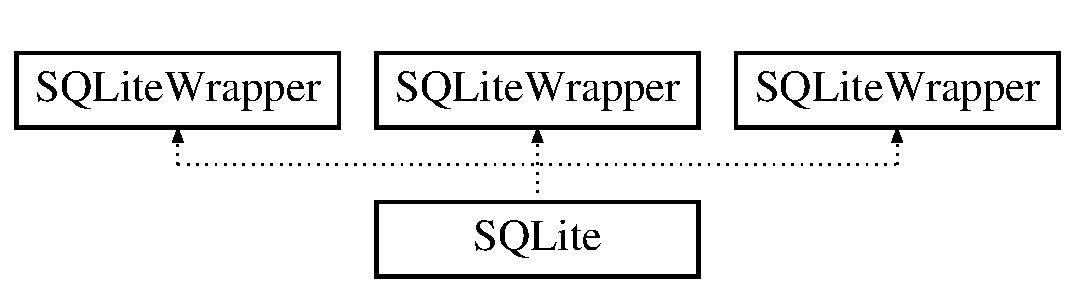
\includegraphics[height=2.000000cm]{d4/dd1/class_s_q_lite}
\end{center}
\end{figure}
\subsection*{Public Member Functions}
\begin{DoxyCompactItemize}
\item 
\mbox{\Hypertarget{class_s_q_lite_a758f334ed7e72820f4f0e83d2b707625}\label{class_s_q_lite_a758f334ed7e72820f4f0e83d2b707625}} 
{\bfseries S\+Q\+Lite} (std\+::string const \&db\+\_\+name, bool init\+\_\+db=false)
\item 
\mbox{\Hypertarget{class_s_q_lite_a0c4fdc189a0da0d879c657b9fed5ef1b}\label{class_s_q_lite_a0c4fdc189a0da0d879c657b9fed5ef1b}} 
std\+::vector$<$ \hyperlink{class_solid_load_charge_material}{Solid\+Load\+Charge\+Material} $>$ {\bfseries get\+Solid\+Load\+Charge\+Materials} () const
\item 
\mbox{\Hypertarget{class_s_q_lite_ab2a00b913321a96a4d7b700627195616}\label{class_s_q_lite_ab2a00b913321a96a4d7b700627195616}} 
\hyperlink{class_solid_load_charge_material}{Solid\+Load\+Charge\+Material} {\bfseries get\+Solid\+Load\+Charge\+Material\+By\+Id} (int id) const
\item 
\mbox{\Hypertarget{class_s_q_lite_a74e20802e333acd20a86bfdc4013eba8}\label{class_s_q_lite_a74e20802e333acd20a86bfdc4013eba8}} 
std\+::vector$<$ \hyperlink{class_solid_load_charge_material}{Solid\+Load\+Charge\+Material} $>$ {\bfseries get\+Custom\+Solid\+Load\+Charge\+Materials} () const
\item 
\mbox{\Hypertarget{class_s_q_lite_a5c40ac3b9a6abb85c9cfbe50802672c5}\label{class_s_q_lite_a5c40ac3b9a6abb85c9cfbe50802672c5}} 
bool {\bfseries insert\+Solid\+Load\+Charge\+Materials} (\hyperlink{class_solid_load_charge_material}{Solid\+Load\+Charge\+Material} const \&material)
\item 
\mbox{\Hypertarget{class_s_q_lite_a0a240c89a1e0c96ef61c3beae68b1467}\label{class_s_q_lite_a0a240c89a1e0c96ef61c3beae68b1467}} 
bool {\bfseries delete\+Solid\+Load\+Charge\+Material} (int id)
\item 
\mbox{\Hypertarget{class_s_q_lite_ac2c7142caa0154783f7ed73afa4bd6db}\label{class_s_q_lite_ac2c7142caa0154783f7ed73afa4bd6db}} 
bool {\bfseries update\+Solid\+Load\+Charge\+Material} (\hyperlink{class_solid_load_charge_material}{Solid\+Load\+Charge\+Material} const \&material)
\item 
\mbox{\Hypertarget{class_s_q_lite_a173cb741ec36f8b15e3650f6e1736b12}\label{class_s_q_lite_a173cb741ec36f8b15e3650f6e1736b12}} 
std\+::vector$<$ \hyperlink{class_gas_load_charge_material}{Gas\+Load\+Charge\+Material} $>$ {\bfseries get\+Gas\+Load\+Charge\+Materials} () const
\item 
\mbox{\Hypertarget{class_s_q_lite_ab89ac4049cbedcb6340f5d7d0139b89e}\label{class_s_q_lite_ab89ac4049cbedcb6340f5d7d0139b89e}} 
\hyperlink{class_gas_load_charge_material}{Gas\+Load\+Charge\+Material} {\bfseries get\+Gas\+Load\+Charge\+Material\+By\+Id} (int id) const
\item 
\mbox{\Hypertarget{class_s_q_lite_a2491f6b082059bde751dfd117f1feed6}\label{class_s_q_lite_a2491f6b082059bde751dfd117f1feed6}} 
std\+::vector$<$ \hyperlink{class_gas_load_charge_material}{Gas\+Load\+Charge\+Material} $>$ {\bfseries get\+Custom\+Gas\+Load\+Charge\+Materials} () const
\item 
\mbox{\Hypertarget{class_s_q_lite_af482f51c0d3de08fbfa3e537382a567f}\label{class_s_q_lite_af482f51c0d3de08fbfa3e537382a567f}} 
bool {\bfseries insert\+Gas\+Load\+Charge\+Materials} (\hyperlink{class_gas_load_charge_material}{Gas\+Load\+Charge\+Material} const \&material)
\item 
\mbox{\Hypertarget{class_s_q_lite_a3717a443c1151d717168d323ec6576c1}\label{class_s_q_lite_a3717a443c1151d717168d323ec6576c1}} 
bool {\bfseries delete\+Gas\+Load\+Charge\+Material} (int id)
\item 
\mbox{\Hypertarget{class_s_q_lite_a21b8fbcd52ac37fe9e78df164ee8de25}\label{class_s_q_lite_a21b8fbcd52ac37fe9e78df164ee8de25}} 
bool {\bfseries update\+Gas\+Load\+Charge\+Material} (const \hyperlink{class_gas_load_charge_material}{Gas\+Load\+Charge\+Material} \&material)
\item 
\mbox{\Hypertarget{class_s_q_lite_a375614ae9d9748646cba88c834796272}\label{class_s_q_lite_a375614ae9d9748646cba88c834796272}} 
std\+::vector$<$ \hyperlink{class_liquid_load_charge_material}{Liquid\+Load\+Charge\+Material} $>$ {\bfseries get\+Liquid\+Load\+Charge\+Materials} () const
\item 
\mbox{\Hypertarget{class_s_q_lite_a3f31756b0fc49be7123e7146cbb12c70}\label{class_s_q_lite_a3f31756b0fc49be7123e7146cbb12c70}} 
\hyperlink{class_liquid_load_charge_material}{Liquid\+Load\+Charge\+Material} {\bfseries get\+Liquid\+Load\+Charge\+Material\+By\+Id} (int id) const
\item 
\mbox{\Hypertarget{class_s_q_lite_aaebe47614c69a50c86a5f585e7b8305c}\label{class_s_q_lite_aaebe47614c69a50c86a5f585e7b8305c}} 
std\+::vector$<$ \hyperlink{class_liquid_load_charge_material}{Liquid\+Load\+Charge\+Material} $>$ {\bfseries get\+Custom\+Liquid\+Load\+Charge\+Materials} () const
\item 
\mbox{\Hypertarget{class_s_q_lite_aff9ccdb8af003d3a0a3fdc9a85af77d8}\label{class_s_q_lite_aff9ccdb8af003d3a0a3fdc9a85af77d8}} 
bool {\bfseries insert\+Liquid\+Load\+Charge\+Materials} (\hyperlink{class_liquid_load_charge_material}{Liquid\+Load\+Charge\+Material} const \&material)
\item 
\mbox{\Hypertarget{class_s_q_lite_a2a3451cb60446d9a90da4cb08920dcfe}\label{class_s_q_lite_a2a3451cb60446d9a90da4cb08920dcfe}} 
bool {\bfseries delete\+Liquid\+Load\+Charge\+Material} (int id)
\item 
\mbox{\Hypertarget{class_s_q_lite_a89805e7aeb9d72f5dfa6928aac681eab}\label{class_s_q_lite_a89805e7aeb9d72f5dfa6928aac681eab}} 
bool {\bfseries update\+Liquid\+Load\+Charge\+Material} (const \hyperlink{class_liquid_load_charge_material}{Liquid\+Load\+Charge\+Material} \&material)
\item 
\mbox{\Hypertarget{class_s_q_lite_aeee9b2bce2f489464d7284224a7422c2}\label{class_s_q_lite_aeee9b2bce2f489464d7284224a7422c2}} 
std\+::vector$<$ \hyperlink{class_solid_liquid_flue_gas_material}{Solid\+Liquid\+Flue\+Gas\+Material} $>$ {\bfseries get\+Solid\+Liquid\+Flue\+Gas\+Materials} () const
\item 
\mbox{\Hypertarget{class_s_q_lite_aa7ea5aa679227d695fe38848236281ee}\label{class_s_q_lite_aa7ea5aa679227d695fe38848236281ee}} 
\hyperlink{class_solid_liquid_flue_gas_material}{Solid\+Liquid\+Flue\+Gas\+Material} {\bfseries get\+Solid\+Liquid\+Flue\+Gas\+Material\+By\+Id} (int id) const
\item 
\mbox{\Hypertarget{class_s_q_lite_a6d11d35cd1cca7b271c64131c30dd829}\label{class_s_q_lite_a6d11d35cd1cca7b271c64131c30dd829}} 
std\+::vector$<$ \hyperlink{class_solid_liquid_flue_gas_material}{Solid\+Liquid\+Flue\+Gas\+Material} $>$ {\bfseries get\+Custom\+Solid\+Liquid\+Flue\+Gas\+Materials} () const
\item 
\mbox{\Hypertarget{class_s_q_lite_aa1de7450c37a07dfd0541fdf0dc164ef}\label{class_s_q_lite_aa1de7450c37a07dfd0541fdf0dc164ef}} 
bool {\bfseries insert\+Solid\+Liquid\+Flue\+Gas\+Material} (\hyperlink{class_solid_liquid_flue_gas_material}{Solid\+Liquid\+Flue\+Gas\+Material} const \&material) const
\item 
\mbox{\Hypertarget{class_s_q_lite_ac83353062d75af65c5b01d55570d0ead}\label{class_s_q_lite_ac83353062d75af65c5b01d55570d0ead}} 
bool {\bfseries delete\+Solid\+Liquid\+Flue\+Gas\+Material} (int id)
\item 
\mbox{\Hypertarget{class_s_q_lite_aed13c3aeeef3fdf7f3b2d72b61dd93e8}\label{class_s_q_lite_aed13c3aeeef3fdf7f3b2d72b61dd93e8}} 
bool {\bfseries update\+Solid\+Liquid\+Flue\+Gas\+Material} (\hyperlink{class_solid_liquid_flue_gas_material}{Solid\+Liquid\+Flue\+Gas\+Material} const \&material)
\item 
\mbox{\Hypertarget{class_s_q_lite_af29fd9f5c71efd6fb1d12a9403e1f433}\label{class_s_q_lite_af29fd9f5c71efd6fb1d12a9403e1f433}} 
std\+::vector$<$ \hyperlink{class_gas_compositions}{Gas\+Compositions} $>$ {\bfseries get\+Gas\+Flue\+Gas\+Materials} () const
\item 
\mbox{\Hypertarget{class_s_q_lite_a230049a94b9e2ff84d19fcd5a087954c}\label{class_s_q_lite_a230049a94b9e2ff84d19fcd5a087954c}} 
\hyperlink{class_gas_compositions}{Gas\+Compositions} {\bfseries get\+Gas\+Flue\+Gas\+Material\+By\+Id} (int id) const
\item 
\mbox{\Hypertarget{class_s_q_lite_a702e2e50ec461d7d47ef33990a1c353e}\label{class_s_q_lite_a702e2e50ec461d7d47ef33990a1c353e}} 
std\+::vector$<$ \hyperlink{class_gas_compositions}{Gas\+Compositions} $>$ {\bfseries get\+Custom\+Gas\+Flue\+Gas\+Materials} () const
\item 
\mbox{\Hypertarget{class_s_q_lite_a95d5521ed0de19c979ac9627ae21fbcd}\label{class_s_q_lite_a95d5521ed0de19c979ac9627ae21fbcd}} 
bool {\bfseries insert\+Gas\+Flue\+Gas\+Material} (\hyperlink{class_gas_compositions}{Gas\+Compositions} const \&material) const
\item 
\mbox{\Hypertarget{class_s_q_lite_a12b38db00e6d8bcff8345e7300a67b26}\label{class_s_q_lite_a12b38db00e6d8bcff8345e7300a67b26}} 
bool {\bfseries delete\+Gas\+Flue\+Gas\+Material} (int id)
\item 
\mbox{\Hypertarget{class_s_q_lite_a71c1973e285ccae25b7bb8dbc101770e}\label{class_s_q_lite_a71c1973e285ccae25b7bb8dbc101770e}} 
bool {\bfseries update\+Gas\+Flue\+Gas\+Material} (\hyperlink{class_gas_compositions}{Gas\+Compositions} const \&material)
\item 
\mbox{\Hypertarget{class_s_q_lite_ab3519768b6490be3ea5c57df3a4ad3a4}\label{class_s_q_lite_ab3519768b6490be3ea5c57df3a4ad3a4}} 
std\+::vector$<$ \hyperlink{class_atmosphere}{Atmosphere} $>$ {\bfseries get\+Atmosphere\+Specific\+Heat} () const
\item 
\mbox{\Hypertarget{class_s_q_lite_ae468835cffed182bb9819299463c53b7}\label{class_s_q_lite_ae468835cffed182bb9819299463c53b7}} 
\hyperlink{class_atmosphere}{Atmosphere} {\bfseries get\+Atmosphere\+Specific\+Heat\+By\+Id} (int id) const
\item 
\mbox{\Hypertarget{class_s_q_lite_a93535b59e35ada6a194601e36c0055f1}\label{class_s_q_lite_a93535b59e35ada6a194601e36c0055f1}} 
std\+::vector$<$ \hyperlink{class_atmosphere}{Atmosphere} $>$ {\bfseries get\+Custom\+Atmosphere\+Specific\+Heat} () const
\item 
\mbox{\Hypertarget{class_s_q_lite_a5be90371486d63abd80668c19682051b}\label{class_s_q_lite_a5be90371486d63abd80668c19682051b}} 
bool {\bfseries insert\+Atmosphere\+Specific\+Heat} (\hyperlink{class_atmosphere}{Atmosphere} const \&material)
\item 
\mbox{\Hypertarget{class_s_q_lite_a0980ef2dfdaadb27f86342f983019bb7}\label{class_s_q_lite_a0980ef2dfdaadb27f86342f983019bb7}} 
bool {\bfseries update\+Atmosphere\+Specific\+Heat} (\hyperlink{class_atmosphere}{Atmosphere} const \&material)
\item 
\mbox{\Hypertarget{class_s_q_lite_a32f61e2c425864cf222ee427abd33448}\label{class_s_q_lite_a32f61e2c425864cf222ee427abd33448}} 
bool {\bfseries delete\+Atmosphere\+Specific\+Heat} (int id)
\item 
\mbox{\Hypertarget{class_s_q_lite_a612950dca9d08332a31a020783ba832d}\label{class_s_q_lite_a612950dca9d08332a31a020783ba832d}} 
std\+::vector$<$ \hyperlink{class_wall_losses}{Wall\+Losses} $>$ {\bfseries get\+Wall\+Losses\+Surface} () const
\item 
\mbox{\Hypertarget{class_s_q_lite_a0314139eab40caf617a2e8e465ba3913}\label{class_s_q_lite_a0314139eab40caf617a2e8e465ba3913}} 
std\+::vector$<$ \hyperlink{class_wall_losses}{Wall\+Losses} $>$ {\bfseries get\+Custom\+Wall\+Losses\+Surface} () const
\item 
\mbox{\Hypertarget{class_s_q_lite_a3a7f473d8e23630dae65cd3c3dd7fa97}\label{class_s_q_lite_a3a7f473d8e23630dae65cd3c3dd7fa97}} 
\hyperlink{class_wall_losses}{Wall\+Losses} {\bfseries get\+Wall\+Losses\+Surface\+By\+Id} (int id) const
\item 
\mbox{\Hypertarget{class_s_q_lite_a97d510f6f16aa70c61a9dc6a629ad786}\label{class_s_q_lite_a97d510f6f16aa70c61a9dc6a629ad786}} 
bool {\bfseries insert\+Wall\+Losses\+Surface} (\hyperlink{class_wall_losses}{Wall\+Losses} const \&material)
\item 
\mbox{\Hypertarget{class_s_q_lite_ab9492a672cb89dfeae330b99ea03ceeb}\label{class_s_q_lite_ab9492a672cb89dfeae330b99ea03ceeb}} 
bool {\bfseries delete\+Wall\+Losses\+Surface} (int id)
\item 
\mbox{\Hypertarget{class_s_q_lite_ac4b7397ef51a0544d38f670ef995f26e}\label{class_s_q_lite_ac4b7397ef51a0544d38f670ef995f26e}} 
bool {\bfseries update\+Wall\+Losses\+Surface} (\hyperlink{class_wall_losses}{Wall\+Losses} const \&material)
\item 
\mbox{\Hypertarget{class_s_q_lite_a5fabd8387b0009f7641bce38ee8e41c5}\label{class_s_q_lite_a5fabd8387b0009f7641bce38ee8e41c5}} 
std\+::vector$<$ \hyperlink{class_motor_data}{Motor\+Data} $>$ {\bfseries get\+Motor\+Data} () const
\item 
\mbox{\Hypertarget{class_s_q_lite_a0cc4f6952652d05d6a87e2f7cc232d57}\label{class_s_q_lite_a0cc4f6952652d05d6a87e2f7cc232d57}} 
std\+::vector$<$ \hyperlink{class_motor_data}{Motor\+Data} $>$ {\bfseries get\+Custom\+Motor\+Data} () const
\item 
\mbox{\Hypertarget{class_s_q_lite_a4b0a99992e2909216b40dc499c86a028}\label{class_s_q_lite_a4b0a99992e2909216b40dc499c86a028}} 
\hyperlink{class_motor_data}{Motor\+Data} {\bfseries get\+Motor\+Data\+By\+Id} (int id) const
\item 
\mbox{\Hypertarget{class_s_q_lite_a38eb0f1501e0918c267a9ab3a0953a54}\label{class_s_q_lite_a38eb0f1501e0918c267a9ab3a0953a54}} 
bool {\bfseries insert\+Motor\+Data} (\hyperlink{class_motor_data}{Motor\+Data} const \&motor)
\item 
\mbox{\Hypertarget{class_s_q_lite_ab1f59cd24e3931970bc39079b0a5e612}\label{class_s_q_lite_ab1f59cd24e3931970bc39079b0a5e612}} 
bool {\bfseries delete\+Motor\+Data} (int id)
\item 
\mbox{\Hypertarget{class_s_q_lite_a7909128eed1b0612ecdf7c50edf1426a}\label{class_s_q_lite_a7909128eed1b0612ecdf7c50edf1426a}} 
bool {\bfseries update\+Motor\+Data} (\hyperlink{class_motor_data}{Motor\+Data} const \&motor)
\item 
\mbox{\Hypertarget{class_s_q_lite_a758f334ed7e72820f4f0e83d2b707625}\label{class_s_q_lite_a758f334ed7e72820f4f0e83d2b707625}} 
{\bfseries S\+Q\+Lite} (std\+::string const \&db\+\_\+name, bool init\+\_\+db=false)
\item 
\mbox{\Hypertarget{class_s_q_lite_af6195f55e9658c24a8f14b884e490acb}\label{class_s_q_lite_af6195f55e9658c24a8f14b884e490acb}} 
std\+::vector$<$ \hyperlink{class_solid_load_charge_material}{Solid\+Load\+Charge\+Material} $>$ {\bfseries get\+Solid\+Load\+Charge\+Materials} () const
\item 
\mbox{\Hypertarget{class_s_q_lite_ab2a00b913321a96a4d7b700627195616}\label{class_s_q_lite_ab2a00b913321a96a4d7b700627195616}} 
\hyperlink{class_solid_load_charge_material}{Solid\+Load\+Charge\+Material} {\bfseries get\+Solid\+Load\+Charge\+Material\+By\+Id} (int id) const
\item 
\mbox{\Hypertarget{class_s_q_lite_a868c571d80d43a991762ec20c168ebb2}\label{class_s_q_lite_a868c571d80d43a991762ec20c168ebb2}} 
std\+::vector$<$ \hyperlink{class_solid_load_charge_material}{Solid\+Load\+Charge\+Material} $>$ {\bfseries get\+Custom\+Solid\+Load\+Charge\+Materials} () const
\item 
\mbox{\Hypertarget{class_s_q_lite_a5c40ac3b9a6abb85c9cfbe50802672c5}\label{class_s_q_lite_a5c40ac3b9a6abb85c9cfbe50802672c5}} 
bool {\bfseries insert\+Solid\+Load\+Charge\+Materials} (\hyperlink{class_solid_load_charge_material}{Solid\+Load\+Charge\+Material} const \&material)
\item 
\mbox{\Hypertarget{class_s_q_lite_a0a240c89a1e0c96ef61c3beae68b1467}\label{class_s_q_lite_a0a240c89a1e0c96ef61c3beae68b1467}} 
bool {\bfseries delete\+Solid\+Load\+Charge\+Material} (int id)
\item 
\mbox{\Hypertarget{class_s_q_lite_ac2c7142caa0154783f7ed73afa4bd6db}\label{class_s_q_lite_ac2c7142caa0154783f7ed73afa4bd6db}} 
bool {\bfseries update\+Solid\+Load\+Charge\+Material} (\hyperlink{class_solid_load_charge_material}{Solid\+Load\+Charge\+Material} const \&material)
\item 
\mbox{\Hypertarget{class_s_q_lite_accd7e97b19298b75eabc3a2b4bbc9b1c}\label{class_s_q_lite_accd7e97b19298b75eabc3a2b4bbc9b1c}} 
std\+::vector$<$ \hyperlink{class_gas_load_charge_material}{Gas\+Load\+Charge\+Material} $>$ {\bfseries get\+Gas\+Load\+Charge\+Materials} () const
\item 
\mbox{\Hypertarget{class_s_q_lite_ab89ac4049cbedcb6340f5d7d0139b89e}\label{class_s_q_lite_ab89ac4049cbedcb6340f5d7d0139b89e}} 
\hyperlink{class_gas_load_charge_material}{Gas\+Load\+Charge\+Material} {\bfseries get\+Gas\+Load\+Charge\+Material\+By\+Id} (int id) const
\item 
\mbox{\Hypertarget{class_s_q_lite_a1957d2f9ac35433b45e8511aa6889756}\label{class_s_q_lite_a1957d2f9ac35433b45e8511aa6889756}} 
std\+::vector$<$ \hyperlink{class_gas_load_charge_material}{Gas\+Load\+Charge\+Material} $>$ {\bfseries get\+Custom\+Gas\+Load\+Charge\+Materials} () const
\item 
\mbox{\Hypertarget{class_s_q_lite_af482f51c0d3de08fbfa3e537382a567f}\label{class_s_q_lite_af482f51c0d3de08fbfa3e537382a567f}} 
bool {\bfseries insert\+Gas\+Load\+Charge\+Materials} (\hyperlink{class_gas_load_charge_material}{Gas\+Load\+Charge\+Material} const \&material)
\item 
\mbox{\Hypertarget{class_s_q_lite_a3717a443c1151d717168d323ec6576c1}\label{class_s_q_lite_a3717a443c1151d717168d323ec6576c1}} 
bool {\bfseries delete\+Gas\+Load\+Charge\+Material} (int id)
\item 
\mbox{\Hypertarget{class_s_q_lite_a21b8fbcd52ac37fe9e78df164ee8de25}\label{class_s_q_lite_a21b8fbcd52ac37fe9e78df164ee8de25}} 
bool {\bfseries update\+Gas\+Load\+Charge\+Material} (const \hyperlink{class_gas_load_charge_material}{Gas\+Load\+Charge\+Material} \&material)
\item 
\mbox{\Hypertarget{class_s_q_lite_a349f65213cc1b022293bc00ba0a4c3b5}\label{class_s_q_lite_a349f65213cc1b022293bc00ba0a4c3b5}} 
std\+::vector$<$ \hyperlink{class_liquid_load_charge_material}{Liquid\+Load\+Charge\+Material} $>$ {\bfseries get\+Liquid\+Load\+Charge\+Materials} () const
\item 
\mbox{\Hypertarget{class_s_q_lite_a3f31756b0fc49be7123e7146cbb12c70}\label{class_s_q_lite_a3f31756b0fc49be7123e7146cbb12c70}} 
\hyperlink{class_liquid_load_charge_material}{Liquid\+Load\+Charge\+Material} {\bfseries get\+Liquid\+Load\+Charge\+Material\+By\+Id} (int id) const
\item 
\mbox{\Hypertarget{class_s_q_lite_a1a252d50bc2e861325f120a814fddd37}\label{class_s_q_lite_a1a252d50bc2e861325f120a814fddd37}} 
std\+::vector$<$ \hyperlink{class_liquid_load_charge_material}{Liquid\+Load\+Charge\+Material} $>$ {\bfseries get\+Custom\+Liquid\+Load\+Charge\+Materials} () const
\item 
\mbox{\Hypertarget{class_s_q_lite_aff9ccdb8af003d3a0a3fdc9a85af77d8}\label{class_s_q_lite_aff9ccdb8af003d3a0a3fdc9a85af77d8}} 
bool {\bfseries insert\+Liquid\+Load\+Charge\+Materials} (\hyperlink{class_liquid_load_charge_material}{Liquid\+Load\+Charge\+Material} const \&material)
\item 
\mbox{\Hypertarget{class_s_q_lite_a2a3451cb60446d9a90da4cb08920dcfe}\label{class_s_q_lite_a2a3451cb60446d9a90da4cb08920dcfe}} 
bool {\bfseries delete\+Liquid\+Load\+Charge\+Material} (int id)
\item 
\mbox{\Hypertarget{class_s_q_lite_a89805e7aeb9d72f5dfa6928aac681eab}\label{class_s_q_lite_a89805e7aeb9d72f5dfa6928aac681eab}} 
bool {\bfseries update\+Liquid\+Load\+Charge\+Material} (const \hyperlink{class_liquid_load_charge_material}{Liquid\+Load\+Charge\+Material} \&material)
\item 
\mbox{\Hypertarget{class_s_q_lite_aecba5bffe035af787b17b5bf5997d825}\label{class_s_q_lite_aecba5bffe035af787b17b5bf5997d825}} 
std\+::vector$<$ \hyperlink{class_solid_liquid_flue_gas_material}{Solid\+Liquid\+Flue\+Gas\+Material} $>$ {\bfseries get\+Solid\+Liquid\+Flue\+Gas\+Materials} () const
\item 
\mbox{\Hypertarget{class_s_q_lite_aa7ea5aa679227d695fe38848236281ee}\label{class_s_q_lite_aa7ea5aa679227d695fe38848236281ee}} 
\hyperlink{class_solid_liquid_flue_gas_material}{Solid\+Liquid\+Flue\+Gas\+Material} {\bfseries get\+Solid\+Liquid\+Flue\+Gas\+Material\+By\+Id} (int id) const
\item 
\mbox{\Hypertarget{class_s_q_lite_a23b34dae2fa12690d3718755fc373b42}\label{class_s_q_lite_a23b34dae2fa12690d3718755fc373b42}} 
std\+::vector$<$ \hyperlink{class_solid_liquid_flue_gas_material}{Solid\+Liquid\+Flue\+Gas\+Material} $>$ {\bfseries get\+Custom\+Solid\+Liquid\+Flue\+Gas\+Materials} () const
\item 
\mbox{\Hypertarget{class_s_q_lite_aa1de7450c37a07dfd0541fdf0dc164ef}\label{class_s_q_lite_aa1de7450c37a07dfd0541fdf0dc164ef}} 
bool {\bfseries insert\+Solid\+Liquid\+Flue\+Gas\+Material} (\hyperlink{class_solid_liquid_flue_gas_material}{Solid\+Liquid\+Flue\+Gas\+Material} const \&material) const
\item 
\mbox{\Hypertarget{class_s_q_lite_ac83353062d75af65c5b01d55570d0ead}\label{class_s_q_lite_ac83353062d75af65c5b01d55570d0ead}} 
bool {\bfseries delete\+Solid\+Liquid\+Flue\+Gas\+Material} (int id)
\item 
\mbox{\Hypertarget{class_s_q_lite_aed13c3aeeef3fdf7f3b2d72b61dd93e8}\label{class_s_q_lite_aed13c3aeeef3fdf7f3b2d72b61dd93e8}} 
bool {\bfseries update\+Solid\+Liquid\+Flue\+Gas\+Material} (\hyperlink{class_solid_liquid_flue_gas_material}{Solid\+Liquid\+Flue\+Gas\+Material} const \&material)
\item 
\mbox{\Hypertarget{class_s_q_lite_a7f054c9a3a3954277c5de8d4048a40f9}\label{class_s_q_lite_a7f054c9a3a3954277c5de8d4048a40f9}} 
std\+::vector$<$ \hyperlink{class_gas_compositions}{Gas\+Compositions} $>$ {\bfseries get\+Gas\+Flue\+Gas\+Materials} () const
\item 
\mbox{\Hypertarget{class_s_q_lite_a230049a94b9e2ff84d19fcd5a087954c}\label{class_s_q_lite_a230049a94b9e2ff84d19fcd5a087954c}} 
\hyperlink{class_gas_compositions}{Gas\+Compositions} {\bfseries get\+Gas\+Flue\+Gas\+Material\+By\+Id} (int id) const
\item 
\mbox{\Hypertarget{class_s_q_lite_a8cd9d62714f1083bab16e388dabc59be}\label{class_s_q_lite_a8cd9d62714f1083bab16e388dabc59be}} 
std\+::vector$<$ \hyperlink{class_gas_compositions}{Gas\+Compositions} $>$ {\bfseries get\+Custom\+Gas\+Flue\+Gas\+Materials} () const
\item 
\mbox{\Hypertarget{class_s_q_lite_a95d5521ed0de19c979ac9627ae21fbcd}\label{class_s_q_lite_a95d5521ed0de19c979ac9627ae21fbcd}} 
bool {\bfseries insert\+Gas\+Flue\+Gas\+Material} (\hyperlink{class_gas_compositions}{Gas\+Compositions} const \&material) const
\item 
\mbox{\Hypertarget{class_s_q_lite_a12b38db00e6d8bcff8345e7300a67b26}\label{class_s_q_lite_a12b38db00e6d8bcff8345e7300a67b26}} 
bool {\bfseries delete\+Gas\+Flue\+Gas\+Material} (int id)
\item 
\mbox{\Hypertarget{class_s_q_lite_a71c1973e285ccae25b7bb8dbc101770e}\label{class_s_q_lite_a71c1973e285ccae25b7bb8dbc101770e}} 
bool {\bfseries update\+Gas\+Flue\+Gas\+Material} (\hyperlink{class_gas_compositions}{Gas\+Compositions} const \&material)
\item 
\mbox{\Hypertarget{class_s_q_lite_a04d22b056b51fb07d192833806eabdfc}\label{class_s_q_lite_a04d22b056b51fb07d192833806eabdfc}} 
std\+::vector$<$ \hyperlink{class_atmosphere}{Atmosphere} $>$ {\bfseries get\+Atmosphere\+Specific\+Heat} () const
\item 
\mbox{\Hypertarget{class_s_q_lite_ae468835cffed182bb9819299463c53b7}\label{class_s_q_lite_ae468835cffed182bb9819299463c53b7}} 
\hyperlink{class_atmosphere}{Atmosphere} {\bfseries get\+Atmosphere\+Specific\+Heat\+By\+Id} (int id) const
\item 
\mbox{\Hypertarget{class_s_q_lite_adecfb81514a3fa09237baa50b2edf5e7}\label{class_s_q_lite_adecfb81514a3fa09237baa50b2edf5e7}} 
std\+::vector$<$ \hyperlink{class_atmosphere}{Atmosphere} $>$ {\bfseries get\+Custom\+Atmosphere\+Specific\+Heat} () const
\item 
\mbox{\Hypertarget{class_s_q_lite_a5be90371486d63abd80668c19682051b}\label{class_s_q_lite_a5be90371486d63abd80668c19682051b}} 
bool {\bfseries insert\+Atmosphere\+Specific\+Heat} (\hyperlink{class_atmosphere}{Atmosphere} const \&material)
\item 
\mbox{\Hypertarget{class_s_q_lite_a0980ef2dfdaadb27f86342f983019bb7}\label{class_s_q_lite_a0980ef2dfdaadb27f86342f983019bb7}} 
bool {\bfseries update\+Atmosphere\+Specific\+Heat} (\hyperlink{class_atmosphere}{Atmosphere} const \&material)
\item 
\mbox{\Hypertarget{class_s_q_lite_a32f61e2c425864cf222ee427abd33448}\label{class_s_q_lite_a32f61e2c425864cf222ee427abd33448}} 
bool {\bfseries delete\+Atmosphere\+Specific\+Heat} (int id)
\item 
\mbox{\Hypertarget{class_s_q_lite_ac385b0462588b7a18349d1621ceac57c}\label{class_s_q_lite_ac385b0462588b7a18349d1621ceac57c}} 
std\+::vector$<$ \hyperlink{class_wall_losses}{Wall\+Losses} $>$ {\bfseries get\+Wall\+Losses\+Surface} () const
\item 
\mbox{\Hypertarget{class_s_q_lite_aaf414f89916731a94d8c81a98d36987d}\label{class_s_q_lite_aaf414f89916731a94d8c81a98d36987d}} 
std\+::vector$<$ \hyperlink{class_wall_losses}{Wall\+Losses} $>$ {\bfseries get\+Custom\+Wall\+Losses\+Surface} () const
\item 
\mbox{\Hypertarget{class_s_q_lite_a3a7f473d8e23630dae65cd3c3dd7fa97}\label{class_s_q_lite_a3a7f473d8e23630dae65cd3c3dd7fa97}} 
\hyperlink{class_wall_losses}{Wall\+Losses} {\bfseries get\+Wall\+Losses\+Surface\+By\+Id} (int id) const
\item 
\mbox{\Hypertarget{class_s_q_lite_a97d510f6f16aa70c61a9dc6a629ad786}\label{class_s_q_lite_a97d510f6f16aa70c61a9dc6a629ad786}} 
bool {\bfseries insert\+Wall\+Losses\+Surface} (\hyperlink{class_wall_losses}{Wall\+Losses} const \&material)
\item 
\mbox{\Hypertarget{class_s_q_lite_ab9492a672cb89dfeae330b99ea03ceeb}\label{class_s_q_lite_ab9492a672cb89dfeae330b99ea03ceeb}} 
bool {\bfseries delete\+Wall\+Losses\+Surface} (int id)
\item 
\mbox{\Hypertarget{class_s_q_lite_ac4b7397ef51a0544d38f670ef995f26e}\label{class_s_q_lite_ac4b7397ef51a0544d38f670ef995f26e}} 
bool {\bfseries update\+Wall\+Losses\+Surface} (\hyperlink{class_wall_losses}{Wall\+Losses} const \&material)
\item 
\mbox{\Hypertarget{class_s_q_lite_a654ac1320d5629702346f55f99a648c9}\label{class_s_q_lite_a654ac1320d5629702346f55f99a648c9}} 
std\+::vector$<$ \hyperlink{class_motor_data}{Motor\+Data} $>$ {\bfseries get\+Motor\+Data} () const
\item 
\mbox{\Hypertarget{class_s_q_lite_a40f0107a78cdb8d735242d954da87ac7}\label{class_s_q_lite_a40f0107a78cdb8d735242d954da87ac7}} 
std\+::vector$<$ \hyperlink{class_motor_data}{Motor\+Data} $>$ {\bfseries get\+Custom\+Motor\+Data} () const
\item 
\mbox{\Hypertarget{class_s_q_lite_a4b0a99992e2909216b40dc499c86a028}\label{class_s_q_lite_a4b0a99992e2909216b40dc499c86a028}} 
\hyperlink{class_motor_data}{Motor\+Data} {\bfseries get\+Motor\+Data\+By\+Id} (int id) const
\item 
\mbox{\Hypertarget{class_s_q_lite_a38eb0f1501e0918c267a9ab3a0953a54}\label{class_s_q_lite_a38eb0f1501e0918c267a9ab3a0953a54}} 
bool {\bfseries insert\+Motor\+Data} (\hyperlink{class_motor_data}{Motor\+Data} const \&motor)
\item 
\mbox{\Hypertarget{class_s_q_lite_ab1f59cd24e3931970bc39079b0a5e612}\label{class_s_q_lite_ab1f59cd24e3931970bc39079b0a5e612}} 
bool {\bfseries delete\+Motor\+Data} (int id)
\item 
\mbox{\Hypertarget{class_s_q_lite_a7909128eed1b0612ecdf7c50edf1426a}\label{class_s_q_lite_a7909128eed1b0612ecdf7c50edf1426a}} 
bool {\bfseries update\+Motor\+Data} (\hyperlink{class_motor_data}{Motor\+Data} const \&motor)
\item 
\mbox{\Hypertarget{class_s_q_lite_a758f334ed7e72820f4f0e83d2b707625}\label{class_s_q_lite_a758f334ed7e72820f4f0e83d2b707625}} 
{\bfseries S\+Q\+Lite} (std\+::string const \&db\+\_\+name, bool init\+\_\+db=false)
\item 
\mbox{\Hypertarget{class_s_q_lite_af6195f55e9658c24a8f14b884e490acb}\label{class_s_q_lite_af6195f55e9658c24a8f14b884e490acb}} 
std\+::vector$<$ \hyperlink{class_solid_load_charge_material}{Solid\+Load\+Charge\+Material} $>$ {\bfseries get\+Solid\+Load\+Charge\+Materials} () const
\item 
\mbox{\Hypertarget{class_s_q_lite_ab2a00b913321a96a4d7b700627195616}\label{class_s_q_lite_ab2a00b913321a96a4d7b700627195616}} 
\hyperlink{class_solid_load_charge_material}{Solid\+Load\+Charge\+Material} {\bfseries get\+Solid\+Load\+Charge\+Material\+By\+Id} (int id) const
\item 
\mbox{\Hypertarget{class_s_q_lite_a868c571d80d43a991762ec20c168ebb2}\label{class_s_q_lite_a868c571d80d43a991762ec20c168ebb2}} 
std\+::vector$<$ \hyperlink{class_solid_load_charge_material}{Solid\+Load\+Charge\+Material} $>$ {\bfseries get\+Custom\+Solid\+Load\+Charge\+Materials} () const
\item 
\mbox{\Hypertarget{class_s_q_lite_a5c40ac3b9a6abb85c9cfbe50802672c5}\label{class_s_q_lite_a5c40ac3b9a6abb85c9cfbe50802672c5}} 
bool {\bfseries insert\+Solid\+Load\+Charge\+Materials} (\hyperlink{class_solid_load_charge_material}{Solid\+Load\+Charge\+Material} const \&material)
\item 
\mbox{\Hypertarget{class_s_q_lite_a0a240c89a1e0c96ef61c3beae68b1467}\label{class_s_q_lite_a0a240c89a1e0c96ef61c3beae68b1467}} 
bool {\bfseries delete\+Solid\+Load\+Charge\+Material} (int id)
\item 
\mbox{\Hypertarget{class_s_q_lite_ac2c7142caa0154783f7ed73afa4bd6db}\label{class_s_q_lite_ac2c7142caa0154783f7ed73afa4bd6db}} 
bool {\bfseries update\+Solid\+Load\+Charge\+Material} (\hyperlink{class_solid_load_charge_material}{Solid\+Load\+Charge\+Material} const \&material)
\item 
\mbox{\Hypertarget{class_s_q_lite_accd7e97b19298b75eabc3a2b4bbc9b1c}\label{class_s_q_lite_accd7e97b19298b75eabc3a2b4bbc9b1c}} 
std\+::vector$<$ \hyperlink{class_gas_load_charge_material}{Gas\+Load\+Charge\+Material} $>$ {\bfseries get\+Gas\+Load\+Charge\+Materials} () const
\item 
\mbox{\Hypertarget{class_s_q_lite_ab89ac4049cbedcb6340f5d7d0139b89e}\label{class_s_q_lite_ab89ac4049cbedcb6340f5d7d0139b89e}} 
\hyperlink{class_gas_load_charge_material}{Gas\+Load\+Charge\+Material} {\bfseries get\+Gas\+Load\+Charge\+Material\+By\+Id} (int id) const
\item 
\mbox{\Hypertarget{class_s_q_lite_a1957d2f9ac35433b45e8511aa6889756}\label{class_s_q_lite_a1957d2f9ac35433b45e8511aa6889756}} 
std\+::vector$<$ \hyperlink{class_gas_load_charge_material}{Gas\+Load\+Charge\+Material} $>$ {\bfseries get\+Custom\+Gas\+Load\+Charge\+Materials} () const
\item 
\mbox{\Hypertarget{class_s_q_lite_af482f51c0d3de08fbfa3e537382a567f}\label{class_s_q_lite_af482f51c0d3de08fbfa3e537382a567f}} 
bool {\bfseries insert\+Gas\+Load\+Charge\+Materials} (\hyperlink{class_gas_load_charge_material}{Gas\+Load\+Charge\+Material} const \&material)
\item 
\mbox{\Hypertarget{class_s_q_lite_a3717a443c1151d717168d323ec6576c1}\label{class_s_q_lite_a3717a443c1151d717168d323ec6576c1}} 
bool {\bfseries delete\+Gas\+Load\+Charge\+Material} (int id)
\item 
\mbox{\Hypertarget{class_s_q_lite_a21b8fbcd52ac37fe9e78df164ee8de25}\label{class_s_q_lite_a21b8fbcd52ac37fe9e78df164ee8de25}} 
bool {\bfseries update\+Gas\+Load\+Charge\+Material} (const \hyperlink{class_gas_load_charge_material}{Gas\+Load\+Charge\+Material} \&material)
\item 
\mbox{\Hypertarget{class_s_q_lite_a349f65213cc1b022293bc00ba0a4c3b5}\label{class_s_q_lite_a349f65213cc1b022293bc00ba0a4c3b5}} 
std\+::vector$<$ \hyperlink{class_liquid_load_charge_material}{Liquid\+Load\+Charge\+Material} $>$ {\bfseries get\+Liquid\+Load\+Charge\+Materials} () const
\item 
\mbox{\Hypertarget{class_s_q_lite_a3f31756b0fc49be7123e7146cbb12c70}\label{class_s_q_lite_a3f31756b0fc49be7123e7146cbb12c70}} 
\hyperlink{class_liquid_load_charge_material}{Liquid\+Load\+Charge\+Material} {\bfseries get\+Liquid\+Load\+Charge\+Material\+By\+Id} (int id) const
\item 
\mbox{\Hypertarget{class_s_q_lite_a1a252d50bc2e861325f120a814fddd37}\label{class_s_q_lite_a1a252d50bc2e861325f120a814fddd37}} 
std\+::vector$<$ \hyperlink{class_liquid_load_charge_material}{Liquid\+Load\+Charge\+Material} $>$ {\bfseries get\+Custom\+Liquid\+Load\+Charge\+Materials} () const
\item 
\mbox{\Hypertarget{class_s_q_lite_aff9ccdb8af003d3a0a3fdc9a85af77d8}\label{class_s_q_lite_aff9ccdb8af003d3a0a3fdc9a85af77d8}} 
bool {\bfseries insert\+Liquid\+Load\+Charge\+Materials} (\hyperlink{class_liquid_load_charge_material}{Liquid\+Load\+Charge\+Material} const \&material)
\item 
\mbox{\Hypertarget{class_s_q_lite_a2a3451cb60446d9a90da4cb08920dcfe}\label{class_s_q_lite_a2a3451cb60446d9a90da4cb08920dcfe}} 
bool {\bfseries delete\+Liquid\+Load\+Charge\+Material} (int id)
\item 
\mbox{\Hypertarget{class_s_q_lite_a89805e7aeb9d72f5dfa6928aac681eab}\label{class_s_q_lite_a89805e7aeb9d72f5dfa6928aac681eab}} 
bool {\bfseries update\+Liquid\+Load\+Charge\+Material} (const \hyperlink{class_liquid_load_charge_material}{Liquid\+Load\+Charge\+Material} \&material)
\item 
\mbox{\Hypertarget{class_s_q_lite_aecba5bffe035af787b17b5bf5997d825}\label{class_s_q_lite_aecba5bffe035af787b17b5bf5997d825}} 
std\+::vector$<$ \hyperlink{class_solid_liquid_flue_gas_material}{Solid\+Liquid\+Flue\+Gas\+Material} $>$ {\bfseries get\+Solid\+Liquid\+Flue\+Gas\+Materials} () const
\item 
\mbox{\Hypertarget{class_s_q_lite_aa7ea5aa679227d695fe38848236281ee}\label{class_s_q_lite_aa7ea5aa679227d695fe38848236281ee}} 
\hyperlink{class_solid_liquid_flue_gas_material}{Solid\+Liquid\+Flue\+Gas\+Material} {\bfseries get\+Solid\+Liquid\+Flue\+Gas\+Material\+By\+Id} (int id) const
\item 
\mbox{\Hypertarget{class_s_q_lite_a23b34dae2fa12690d3718755fc373b42}\label{class_s_q_lite_a23b34dae2fa12690d3718755fc373b42}} 
std\+::vector$<$ \hyperlink{class_solid_liquid_flue_gas_material}{Solid\+Liquid\+Flue\+Gas\+Material} $>$ {\bfseries get\+Custom\+Solid\+Liquid\+Flue\+Gas\+Materials} () const
\item 
\mbox{\Hypertarget{class_s_q_lite_aa1de7450c37a07dfd0541fdf0dc164ef}\label{class_s_q_lite_aa1de7450c37a07dfd0541fdf0dc164ef}} 
bool {\bfseries insert\+Solid\+Liquid\+Flue\+Gas\+Material} (\hyperlink{class_solid_liquid_flue_gas_material}{Solid\+Liquid\+Flue\+Gas\+Material} const \&material) const
\item 
\mbox{\Hypertarget{class_s_q_lite_ac83353062d75af65c5b01d55570d0ead}\label{class_s_q_lite_ac83353062d75af65c5b01d55570d0ead}} 
bool {\bfseries delete\+Solid\+Liquid\+Flue\+Gas\+Material} (int id)
\item 
\mbox{\Hypertarget{class_s_q_lite_aed13c3aeeef3fdf7f3b2d72b61dd93e8}\label{class_s_q_lite_aed13c3aeeef3fdf7f3b2d72b61dd93e8}} 
bool {\bfseries update\+Solid\+Liquid\+Flue\+Gas\+Material} (\hyperlink{class_solid_liquid_flue_gas_material}{Solid\+Liquid\+Flue\+Gas\+Material} const \&material)
\item 
\mbox{\Hypertarget{class_s_q_lite_a7f054c9a3a3954277c5de8d4048a40f9}\label{class_s_q_lite_a7f054c9a3a3954277c5de8d4048a40f9}} 
std\+::vector$<$ \hyperlink{class_gas_compositions}{Gas\+Compositions} $>$ {\bfseries get\+Gas\+Flue\+Gas\+Materials} () const
\item 
\mbox{\Hypertarget{class_s_q_lite_a230049a94b9e2ff84d19fcd5a087954c}\label{class_s_q_lite_a230049a94b9e2ff84d19fcd5a087954c}} 
\hyperlink{class_gas_compositions}{Gas\+Compositions} {\bfseries get\+Gas\+Flue\+Gas\+Material\+By\+Id} (int id) const
\item 
\mbox{\Hypertarget{class_s_q_lite_a8cd9d62714f1083bab16e388dabc59be}\label{class_s_q_lite_a8cd9d62714f1083bab16e388dabc59be}} 
std\+::vector$<$ \hyperlink{class_gas_compositions}{Gas\+Compositions} $>$ {\bfseries get\+Custom\+Gas\+Flue\+Gas\+Materials} () const
\item 
\mbox{\Hypertarget{class_s_q_lite_a95d5521ed0de19c979ac9627ae21fbcd}\label{class_s_q_lite_a95d5521ed0de19c979ac9627ae21fbcd}} 
bool {\bfseries insert\+Gas\+Flue\+Gas\+Material} (\hyperlink{class_gas_compositions}{Gas\+Compositions} const \&material) const
\item 
\mbox{\Hypertarget{class_s_q_lite_a12b38db00e6d8bcff8345e7300a67b26}\label{class_s_q_lite_a12b38db00e6d8bcff8345e7300a67b26}} 
bool {\bfseries delete\+Gas\+Flue\+Gas\+Material} (int id)
\item 
\mbox{\Hypertarget{class_s_q_lite_a71c1973e285ccae25b7bb8dbc101770e}\label{class_s_q_lite_a71c1973e285ccae25b7bb8dbc101770e}} 
bool {\bfseries update\+Gas\+Flue\+Gas\+Material} (\hyperlink{class_gas_compositions}{Gas\+Compositions} const \&material)
\item 
\mbox{\Hypertarget{class_s_q_lite_a04d22b056b51fb07d192833806eabdfc}\label{class_s_q_lite_a04d22b056b51fb07d192833806eabdfc}} 
std\+::vector$<$ \hyperlink{class_atmosphere}{Atmosphere} $>$ {\bfseries get\+Atmosphere\+Specific\+Heat} () const
\item 
\mbox{\Hypertarget{class_s_q_lite_ae468835cffed182bb9819299463c53b7}\label{class_s_q_lite_ae468835cffed182bb9819299463c53b7}} 
\hyperlink{class_atmosphere}{Atmosphere} {\bfseries get\+Atmosphere\+Specific\+Heat\+By\+Id} (int id) const
\item 
\mbox{\Hypertarget{class_s_q_lite_adecfb81514a3fa09237baa50b2edf5e7}\label{class_s_q_lite_adecfb81514a3fa09237baa50b2edf5e7}} 
std\+::vector$<$ \hyperlink{class_atmosphere}{Atmosphere} $>$ {\bfseries get\+Custom\+Atmosphere\+Specific\+Heat} () const
\item 
\mbox{\Hypertarget{class_s_q_lite_a5be90371486d63abd80668c19682051b}\label{class_s_q_lite_a5be90371486d63abd80668c19682051b}} 
bool {\bfseries insert\+Atmosphere\+Specific\+Heat} (\hyperlink{class_atmosphere}{Atmosphere} const \&material)
\item 
\mbox{\Hypertarget{class_s_q_lite_a0980ef2dfdaadb27f86342f983019bb7}\label{class_s_q_lite_a0980ef2dfdaadb27f86342f983019bb7}} 
bool {\bfseries update\+Atmosphere\+Specific\+Heat} (\hyperlink{class_atmosphere}{Atmosphere} const \&material)
\item 
\mbox{\Hypertarget{class_s_q_lite_a32f61e2c425864cf222ee427abd33448}\label{class_s_q_lite_a32f61e2c425864cf222ee427abd33448}} 
bool {\bfseries delete\+Atmosphere\+Specific\+Heat} (int id)
\item 
\mbox{\Hypertarget{class_s_q_lite_ac385b0462588b7a18349d1621ceac57c}\label{class_s_q_lite_ac385b0462588b7a18349d1621ceac57c}} 
std\+::vector$<$ \hyperlink{class_wall_losses}{Wall\+Losses} $>$ {\bfseries get\+Wall\+Losses\+Surface} () const
\item 
\mbox{\Hypertarget{class_s_q_lite_aaf414f89916731a94d8c81a98d36987d}\label{class_s_q_lite_aaf414f89916731a94d8c81a98d36987d}} 
std\+::vector$<$ \hyperlink{class_wall_losses}{Wall\+Losses} $>$ {\bfseries get\+Custom\+Wall\+Losses\+Surface} () const
\item 
\mbox{\Hypertarget{class_s_q_lite_a3a7f473d8e23630dae65cd3c3dd7fa97}\label{class_s_q_lite_a3a7f473d8e23630dae65cd3c3dd7fa97}} 
\hyperlink{class_wall_losses}{Wall\+Losses} {\bfseries get\+Wall\+Losses\+Surface\+By\+Id} (int id) const
\item 
\mbox{\Hypertarget{class_s_q_lite_a97d510f6f16aa70c61a9dc6a629ad786}\label{class_s_q_lite_a97d510f6f16aa70c61a9dc6a629ad786}} 
bool {\bfseries insert\+Wall\+Losses\+Surface} (\hyperlink{class_wall_losses}{Wall\+Losses} const \&material)
\item 
\mbox{\Hypertarget{class_s_q_lite_ab9492a672cb89dfeae330b99ea03ceeb}\label{class_s_q_lite_ab9492a672cb89dfeae330b99ea03ceeb}} 
bool {\bfseries delete\+Wall\+Losses\+Surface} (int id)
\item 
\mbox{\Hypertarget{class_s_q_lite_ac4b7397ef51a0544d38f670ef995f26e}\label{class_s_q_lite_ac4b7397ef51a0544d38f670ef995f26e}} 
bool {\bfseries update\+Wall\+Losses\+Surface} (\hyperlink{class_wall_losses}{Wall\+Losses} const \&material)
\item 
\mbox{\Hypertarget{class_s_q_lite_a654ac1320d5629702346f55f99a648c9}\label{class_s_q_lite_a654ac1320d5629702346f55f99a648c9}} 
std\+::vector$<$ \hyperlink{class_motor_data}{Motor\+Data} $>$ {\bfseries get\+Motor\+Data} () const
\item 
\mbox{\Hypertarget{class_s_q_lite_a40f0107a78cdb8d735242d954da87ac7}\label{class_s_q_lite_a40f0107a78cdb8d735242d954da87ac7}} 
std\+::vector$<$ \hyperlink{class_motor_data}{Motor\+Data} $>$ {\bfseries get\+Custom\+Motor\+Data} () const
\item 
\mbox{\Hypertarget{class_s_q_lite_a4b0a99992e2909216b40dc499c86a028}\label{class_s_q_lite_a4b0a99992e2909216b40dc499c86a028}} 
\hyperlink{class_motor_data}{Motor\+Data} {\bfseries get\+Motor\+Data\+By\+Id} (int id) const
\item 
\mbox{\Hypertarget{class_s_q_lite_a38eb0f1501e0918c267a9ab3a0953a54}\label{class_s_q_lite_a38eb0f1501e0918c267a9ab3a0953a54}} 
bool {\bfseries insert\+Motor\+Data} (\hyperlink{class_motor_data}{Motor\+Data} const \&motor)
\item 
\mbox{\Hypertarget{class_s_q_lite_ab1f59cd24e3931970bc39079b0a5e612}\label{class_s_q_lite_ab1f59cd24e3931970bc39079b0a5e612}} 
bool {\bfseries delete\+Motor\+Data} (int id)
\item 
\mbox{\Hypertarget{class_s_q_lite_a7909128eed1b0612ecdf7c50edf1426a}\label{class_s_q_lite_a7909128eed1b0612ecdf7c50edf1426a}} 
bool {\bfseries update\+Motor\+Data} (\hyperlink{class_motor_data}{Motor\+Data} const \&motor)
\end{DoxyCompactItemize}


\subsection{Detailed Description}


Definition at line 93 of file S\+Q\+Lite.\+h.



The documentation for this class was generated from the following files\+:\begin{DoxyCompactItemize}
\item 
\+\_\+\+C\+Pack\+\_\+\+Packages/\+Darwin/\+S\+T\+G\+Z/amo\+\_\+tools\+\_\+suite-\/-\/\+Darwin-\/x86\+\_\+64-\/\+Debug/amo\+\_\+tools\+\_\+suite/include/sqlite/S\+Q\+Lite.\+h\item 
\+\_\+\+C\+Pack\+\_\+\+Packages/\+Darwin/\+S\+T\+G\+Z/amo\+\_\+tools\+\_\+suite-\/-\/\+Darwin-\/x86\+\_\+64-\/\+Debug/amo\+\_\+tools\+\_\+suite/include/sqlite/Atmosphere\+Specific\+Heat\+Data.\+h\item 
\+\_\+\+C\+Pack\+\_\+\+Packages/\+Darwin/\+S\+T\+G\+Z/amo\+\_\+tools\+\_\+suite-\/-\/\+Darwin-\/x86\+\_\+64-\/\+Debug/amo\+\_\+tools\+\_\+suite/include/sqlite/Gas\+Flue\+Gas\+Material\+Data.\+h\item 
\+\_\+\+C\+Pack\+\_\+\+Packages/\+Darwin/\+S\+T\+G\+Z/amo\+\_\+tools\+\_\+suite-\/-\/\+Darwin-\/x86\+\_\+64-\/\+Debug/amo\+\_\+tools\+\_\+suite/include/sqlite/Gas\+Load\+Charge\+Material\+Data.\+h\item 
\+\_\+\+C\+Pack\+\_\+\+Packages/\+Darwin/\+S\+T\+G\+Z/amo\+\_\+tools\+\_\+suite-\/-\/\+Darwin-\/x86\+\_\+64-\/\+Debug/amo\+\_\+tools\+\_\+suite/include/sqlite/Liquid\+Load\+Charge\+Material\+Data.\+h\item 
\+\_\+\+C\+Pack\+\_\+\+Packages/\+Darwin/\+S\+T\+G\+Z/amo\+\_\+tools\+\_\+suite-\/-\/\+Darwin-\/x86\+\_\+64-\/\+Debug/amo\+\_\+tools\+\_\+suite/include/sqlite/Motor\+Data.\+h\item 
\+\_\+\+C\+Pack\+\_\+\+Packages/\+Darwin/\+S\+T\+G\+Z/amo\+\_\+tools\+\_\+suite-\/-\/\+Darwin-\/x86\+\_\+64-\/\+Debug/amo\+\_\+tools\+\_\+suite/include/sqlite/Solid\+Liquid\+Flue\+Gas\+Material\+Data.\+h\item 
\+\_\+\+C\+Pack\+\_\+\+Packages/\+Darwin/\+S\+T\+G\+Z/amo\+\_\+tools\+\_\+suite-\/-\/\+Darwin-\/x86\+\_\+64-\/\+Debug/amo\+\_\+tools\+\_\+suite/include/sqlite/Solid\+Load\+Charge\+Material\+Data.\+h\item 
\+\_\+\+C\+Pack\+\_\+\+Packages/\+Darwin/\+S\+T\+G\+Z/amo\+\_\+tools\+\_\+suite-\/-\/\+Darwin-\/x86\+\_\+64-\/\+Debug/amo\+\_\+tools\+\_\+suite/include/sqlite/Wall\+Losses\+Surface\+Data.\+h\item 
src/sqlite/S\+Q\+Lite.\+cpp\end{DoxyCompactItemize}

\hypertarget{class_s_q_lite_wrapper}{}\section{S\+Q\+Lite\+Wrapper Class Reference}
\label{class_s_q_lite_wrapper}\index{S\+Q\+Lite\+Wrapper@{S\+Q\+Lite\+Wrapper}}
Inheritance diagram for S\+Q\+Lite\+Wrapper\+:\begin{figure}[H]
\begin{center}
\leavevmode
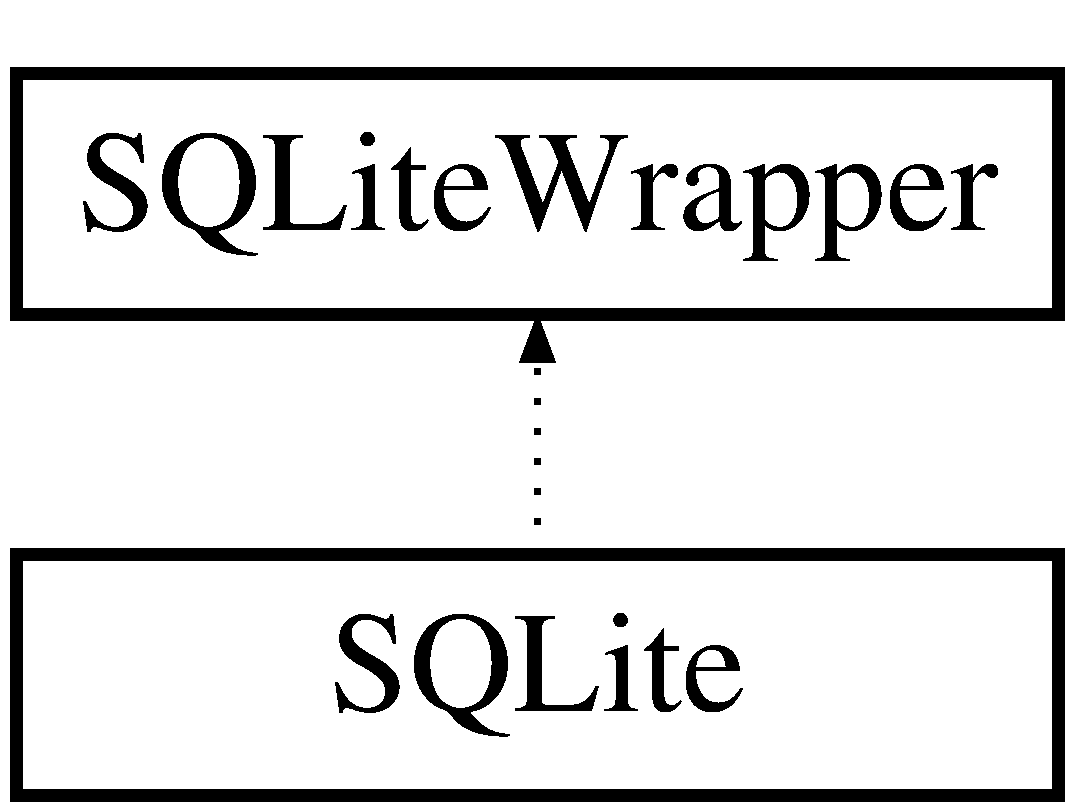
\includegraphics[height=2.000000cm]{da/d65/class_s_q_lite_wrapper}
\end{center}
\end{figure}
\subsection*{Protected Member Functions}
\begin{DoxyCompactItemize}
\item 
\mbox{\Hypertarget{class_s_q_lite_wrapper_a9a61e968f7a892ddb9383fa8db001705}\label{class_s_q_lite_wrapper_a9a61e968f7a892ddb9383fa8db001705}} 
{\bfseries S\+Q\+Lite\+Wrapper} (std\+::shared\+\_\+ptr$<$ sqlite3 $>$ const \&db)
\item 
\mbox{\Hypertarget{class_s_q_lite_wrapper_ae1fce784c6c43a9deea31f68fc2e9966}\label{class_s_q_lite_wrapper_ae1fce784c6c43a9deea31f68fc2e9966}} 
{\bfseries S\+Q\+Lite\+Wrapper} (std\+::string const \&db\+\_\+name, bool init\+\_\+db=false)
\item 
\mbox{\Hypertarget{class_s_q_lite_wrapper_affeef069fe57f5340b64cd5dd41a5b51}\label{class_s_q_lite_wrapper_affeef069fe57f5340b64cd5dd41a5b51}} 
int {\bfseries execute\+\_\+command} (std\+::string const \&command\+\_\+buffer) const
\item 
\mbox{\Hypertarget{class_s_q_lite_wrapper_a8635a805eb0012f6ef97335e003d740f}\label{class_s_q_lite_wrapper_a8635a805eb0012f6ef97335e003d740f}} 
int {\bfseries prepare\+\_\+statement} (sqlite3\+\_\+stmt $\ast$\&stmt, std\+::string const \&stmt\+\_\+buffer) const
\item 
\mbox{\Hypertarget{class_s_q_lite_wrapper_a8cbdaf79201aabb1a70208cd1264b004}\label{class_s_q_lite_wrapper_a8cbdaf79201aabb1a70208cd1264b004}} 
int {\bfseries bind\+\_\+value} (sqlite3\+\_\+stmt $\ast$stmt, int const stmt\+\_\+insert\+\_\+col\+\_\+index, std\+::string const \&text\+\_\+buffer) const
\item 
\mbox{\Hypertarget{class_s_q_lite_wrapper_a3dd12d5bcf5c795ed14d38835b24c8f5}\label{class_s_q_lite_wrapper_a3dd12d5bcf5c795ed14d38835b24c8f5}} 
int {\bfseries bind\+\_\+value} (sqlite3\+\_\+stmt $\ast$stmt, int const stmt\+\_\+insert\+\_\+col\+\_\+index, int const int\+\_\+to\+\_\+insert) const
\item 
\mbox{\Hypertarget{class_s_q_lite_wrapper_ad76118f495723394edf380cf70e0e381}\label{class_s_q_lite_wrapper_ad76118f495723394edf380cf70e0e381}} 
int {\bfseries bind\+\_\+value} (sqlite3\+\_\+stmt $\ast$stmt, int const stmt\+\_\+insert\+\_\+col\+\_\+index, double const double\+\_\+to\+\_\+insert) const
\item 
\mbox{\Hypertarget{class_s_q_lite_wrapper_a3bfa48072fccfb0ab7591f240b468112}\label{class_s_q_lite_wrapper_a3bfa48072fccfb0ab7591f240b468112}} 
int {\bfseries bind\+\_\+value} (sqlite3\+\_\+stmt $\ast$stmt, int const stmt\+\_\+insert\+\_\+col\+\_\+index) const
\item 
\mbox{\Hypertarget{class_s_q_lite_wrapper_a4b6f58f924fae97702115f34ea8abf22}\label{class_s_q_lite_wrapper_a4b6f58f924fae97702115f34ea8abf22}} 
int {\bfseries bind\+\_\+value} (sqlite3\+\_\+stmt $\ast$stmt, int const stmt\+\_\+insert\+\_\+col\+\_\+index, const bool value\+\_\+to\+\_\+insert) const
\item 
\mbox{\Hypertarget{class_s_q_lite_wrapper_a21b4c5733febabb2a4f21772b7cfdec1}\label{class_s_q_lite_wrapper_a21b4c5733febabb2a4f21772b7cfdec1}} 
int {\bfseries bind\+\_\+foreign\+\_\+key} (sqlite3\+\_\+stmt $\ast$stmt, int const stmt\+\_\+insert\+\_\+col\+\_\+index, int const int\+\_\+to\+\_\+insert) const
\item 
\mbox{\Hypertarget{class_s_q_lite_wrapper_a2c0169834d2518ede1f00b92ffbed3e2}\label{class_s_q_lite_wrapper_a2c0169834d2518ede1f00b92ffbed3e2}} 
bool {\bfseries step\+\_\+validity} (int const rc) const
\item 
\mbox{\Hypertarget{class_s_q_lite_wrapper_aed2fd5a33db820461662e6ffdc05808b}\label{class_s_q_lite_wrapper_aed2fd5a33db820461662e6ffdc05808b}} 
int {\bfseries step\+\_\+command} (sqlite3\+\_\+stmt $\ast$stmt) const
\item 
\mbox{\Hypertarget{class_s_q_lite_wrapper_aeef995f134463b92babcd805444a1783}\label{class_s_q_lite_wrapper_aeef995f134463b92babcd805444a1783}} 
int {\bfseries reset\+\_\+command} (sqlite3\+\_\+stmt $\ast$stmt) const
\item 
\mbox{\Hypertarget{class_s_q_lite_wrapper_a7390f800549dbb01bb6bea58f3834c0c}\label{class_s_q_lite_wrapper_a7390f800549dbb01bb6bea58f3834c0c}} 
void {\bfseries begin\+\_\+transaction} () const
\item 
\mbox{\Hypertarget{class_s_q_lite_wrapper_a80905f75cc7115658a61037a4c7a2e62}\label{class_s_q_lite_wrapper_a80905f75cc7115658a61037a4c7a2e62}} 
void {\bfseries commit\+\_\+transaction} () const
\item 
\mbox{\Hypertarget{class_s_q_lite_wrapper_ad729120a855cf8db16940f9798897cc5}\label{class_s_q_lite_wrapper_ad729120a855cf8db16940f9798897cc5}} 
{\footnotesize template$<$typename T $>$ }\\std\+::vector$<$ T $>$ {\bfseries get\+\_\+all\+\_\+objects} (sqlite3\+\_\+stmt $\ast$stmt, std\+::function$<$ T(sqlite3\+\_\+stmt $\ast$) $>$ cb) const
\item 
\mbox{\Hypertarget{class_s_q_lite_wrapper_a7b08d5d170b1c19f7a0be0ecdec4195e}\label{class_s_q_lite_wrapper_a7b08d5d170b1c19f7a0be0ecdec4195e}} 
{\footnotesize template$<$typename T $>$ }\\T {\bfseries get\+\_\+object} (sqlite3\+\_\+stmt $\ast$stmt, int const id, std\+::function$<$ T(sqlite3\+\_\+stmt $\ast$) $>$ cb) const
\end{DoxyCompactItemize}
\subsection*{Static Protected Member Functions}
\begin{DoxyCompactItemize}
\item 
\mbox{\Hypertarget{class_s_q_lite_wrapper_a46a46fe7c7b6887967540721368acd7c}\label{class_s_q_lite_wrapper_a46a46fe7c7b6887967540721368acd7c}} 
static std\+::string {\bfseries convert\+\_\+text} (const unsigned char $\ast$text)
\end{DoxyCompactItemize}


\subsection{Detailed Description}


Definition at line 19 of file S\+Q\+Lite.\+h.



The documentation for this class was generated from the following files\+:\begin{DoxyCompactItemize}
\item 
include/sqlite/S\+Q\+Lite.\+h\item 
src/sqlite/S\+Q\+Lite.\+cpp\end{DoxyCompactItemize}

\hypertarget{class_steam_properties}{}\section{Steam\+Properties Class Reference}
\label{class_steam_properties}\index{Steam\+Properties@{Steam\+Properties}}
\subsection*{Public Types}
\begin{DoxyCompactItemize}
\item 
\mbox{\Hypertarget{class_steam_properties_ae0294bedf7d178c2d8fb6aed0f62fbff}\label{class_steam_properties_ae0294bedf7d178c2d8fb6aed0f62fbff}} 
enum \hyperlink{class_steam_properties_ae0294bedf7d178c2d8fb6aed0f62fbff}{Thermodynamic\+Quantity} \{ {\bfseries T\+E\+M\+P\+E\+R\+A\+T\+U\+RE}, 
{\bfseries E\+N\+T\+H\+A\+L\+PY}, 
{\bfseries E\+N\+T\+R\+O\+PY}, 
{\bfseries Q\+U\+A\+L\+I\+TY}
 \}\begin{DoxyCompactList}\small\item\em enum class for Thermodynamic\+Quantity \end{DoxyCompactList}
\end{DoxyCompactItemize}
\subsection*{Public Member Functions}
\begin{DoxyCompactItemize}
\item 
\hyperlink{class_steam_properties_a976e08ed0433943d469a8c2f75d2ac68}{Steam\+Properties} (const double pressure, const \hyperlink{class_steam_properties_ae0294bedf7d178c2d8fb6aed0f62fbff}{Thermodynamic\+Quantity} quantity, const double quantity\+Value)
\item 
\hyperlink{struct_steam_system_modeler_tool_1_1_steam_properties_output}{Steam\+System\+Modeler\+Tool\+::\+Steam\+Properties\+Output} \hyperlink{class_steam_properties_a8c729e006c34157435d5476fb31e30b5}{calculate} ()
\end{DoxyCompactItemize}


\subsection{Detailed Description}


Definition at line 9 of file Steam\+Properties.\+h.



\subsection{Constructor \& Destructor Documentation}
\mbox{\Hypertarget{class_steam_properties_a976e08ed0433943d469a8c2f75d2ac68}\label{class_steam_properties_a976e08ed0433943d469a8c2f75d2ac68}} 
\index{Steam\+Properties@{Steam\+Properties}!Steam\+Properties@{Steam\+Properties}}
\index{Steam\+Properties@{Steam\+Properties}!Steam\+Properties@{Steam\+Properties}}
\subsubsection{\texorpdfstring{Steam\+Properties()}{SteamProperties()}}
{\footnotesize\ttfamily Steam\+Properties\+::\+Steam\+Properties (\begin{DoxyParamCaption}\item[{const double}]{pressure,  }\item[{const \hyperlink{class_steam_properties_ae0294bedf7d178c2d8fb6aed0f62fbff}{Thermodynamic\+Quantity}}]{quantity,  }\item[{const double}]{quantity\+Value }\end{DoxyParamCaption})\hspace{0.3cm}{\ttfamily [inline]}}

Constructor for \hyperlink{class_steam_properties}{Steam\+Properties} class 
\begin{DoxyParams}{Parameters}
{\em pressure} & double, pressure in M\+Pa \\
\hline
{\em quantity\+Value,Thermodynamic} & Property used for calculation-\/ Temperature (K), Enthalpy (k\+J/kg), Entropy (k\+J/kg-\/K), or Quality (unitless) \\
\hline
{\em quantity} & Thermodynamic\+Quantity, the value type used to calculate steam properties (T\+E\+M\+P\+E\+R\+A\+T\+U\+RE, E\+N\+T\+H\+A\+L\+PY, etc.) \\
\hline
\end{DoxyParams}


Definition at line 26 of file Steam\+Properties.\+h.



\subsection{Member Function Documentation}
\mbox{\Hypertarget{class_steam_properties_a8c729e006c34157435d5476fb31e30b5}\label{class_steam_properties_a8c729e006c34157435d5476fb31e30b5}} 
\index{Steam\+Properties@{Steam\+Properties}!calculate@{calculate}}
\index{calculate@{calculate}!Steam\+Properties@{Steam\+Properties}}
\subsubsection{\texorpdfstring{calculate()}{calculate()}}
{\footnotesize\ttfamily \hyperlink{struct_steam_system_modeler_tool_1_1_steam_properties_output}{Steam\+System\+Modeler\+Tool\+::\+Steam\+Properties\+Output} Steam\+Properties\+::calculate (\begin{DoxyParamCaption}{ }\end{DoxyParamCaption})}

Calculates the steam properties


\begin{DoxyParams}{Parameters}
{\em pressure} & double, pressure in M\+Pa \\
\hline
{\em quantity\+Value} & Thermodynamic\+Quantity, the type of value that will be used to calculate the steam properties (T\+E\+M\+P\+E\+R\+A\+T\+U\+RE,E\+N\+T\+H\+A\+L\+PY, etc.)\\
\hline
\end{DoxyParams}
\begin{DoxyReturn}{Returns}
\hyperlink{struct_steam_system_modeler_tool_1_1_steam_properties_output}{Steam\+System\+Modeler\+Tool\+::\+Steam\+Properties\+Output}, steam properties 
\end{DoxyReturn}


Definition at line 5 of file Steam\+Properties.\+cpp.



The documentation for this class was generated from the following files\+:\begin{DoxyCompactItemize}
\item 
include/ssmt/Steam\+Properties.\+h\item 
src/ssmt/Steam\+Properties.\+cpp\end{DoxyCompactItemize}

\hypertarget{class_steam_system_modeler_tool}{}\section{Steam\+System\+Modeler\+Tool Class Reference}
\label{class_steam_system_modeler_tool}\index{Steam\+System\+Modeler\+Tool@{Steam\+System\+Modeler\+Tool}}
\subsection*{Public Types}
\begin{DoxyCompactItemize}
\item 
\mbox{\Hypertarget{class_steam_system_modeler_tool_aed38516c350ca4ecf17b545e07d41dcd}\label{class_steam_system_modeler_tool_aed38516c350ca4ecf17b545e07d41dcd}} 
enum {\bfseries Key} \{ {\bfseries E\+N\+T\+H\+A\+L\+PY}, 
{\bfseries E\+N\+T\+R\+O\+PY}
 \}
\item 
\mbox{\Hypertarget{class_steam_system_modeler_tool_a162eeadc7eb56a9b50b7a8f630eb8f05}\label{class_steam_system_modeler_tool_a162eeadc7eb56a9b50b7a8f630eb8f05}} 
enum {\bfseries Region} \{ {\bfseries R\+E\+G\+I\+O\+N1}, 
{\bfseries R\+E\+G\+I\+O\+N2A}, 
{\bfseries R\+E\+G\+I\+O\+N2B}, 
{\bfseries R\+E\+G\+I\+O\+N2C}
 \}
\end{DoxyCompactItemize}
\subsection*{Friends}
\begin{DoxyCompactItemize}
\item 
\mbox{\Hypertarget{class_steam_system_modeler_tool_a7b6c56e04b76b2d946235064998e84c9}\label{class_steam_system_modeler_tool_a7b6c56e04b76b2d946235064998e84c9}} 
class {\bfseries Steam\+Properties}
\item 
\mbox{\Hypertarget{class_steam_system_modeler_tool_a43a03ec32145468365cf841d9310263c}\label{class_steam_system_modeler_tool_a43a03ec32145468365cf841d9310263c}} 
class {\bfseries Saturated\+Properties}
\end{DoxyCompactItemize}


\subsection{Detailed Description}


Definition at line 26 of file Steam\+System\+Modeler\+Tool.\+h.



The documentation for this class was generated from the following files\+:\begin{DoxyCompactItemize}
\item 
include/ssmt/Steam\+System\+Modeler\+Tool.\+h\item 
src/ssmt/Steam\+System\+Modeler\+Tool.\+cpp\end{DoxyCompactItemize}

\hypertarget{class_turbine}{}\section{Turbine Class Reference}
\label{class_turbine}\index{Turbine@{Turbine}}
\subsection*{Public Types}
\begin{DoxyCompactItemize}
\item 
\mbox{\Hypertarget{class_turbine_a9fd7beba6c6f071e228fbe3e07969d2b}\label{class_turbine_a9fd7beba6c6f071e228fbe3e07969d2b}} 
enum {\bfseries Solve} \{ {\bfseries Outlet\+Properties}, 
{\bfseries Isentropic\+Efficiency}
 \}
\item 
\mbox{\Hypertarget{class_turbine_a5db4f65cf2539e3837684d53221ade12}\label{class_turbine_a5db4f65cf2539e3837684d53221ade12}} 
enum {\bfseries Turbine\+Property} \{ {\bfseries Mass\+Flow}, 
{\bfseries Power\+Out}
 \}
\end{DoxyCompactItemize}
\subsection*{Public Member Functions}
\begin{DoxyCompactItemize}
\item 
\mbox{\Hypertarget{class_turbine_a3c3c871b9fe57d48dd06b109794381dc}\label{class_turbine_a3c3c871b9fe57d48dd06b109794381dc}} 
{\bfseries Turbine} (Solve solve\+For, double inlet\+Pressure, \hyperlink{class_steam_properties_ae0294bedf7d178c2d8fb6aed0f62fbff}{Steam\+Properties\+::\+Thermodynamic\+Quantity} inlet\+Quantity, double inlet\+Quantity\+Value, Turbine\+Property turbine\+Property, double isentropic\+Efficiency, double generator\+Efficiency, double mass\+Flow\+Or\+Power\+Out, double outlet\+Steam\+Pressure)
\item 
\mbox{\Hypertarget{class_turbine_a1ec182906c075407882de542954d9030}\label{class_turbine_a1ec182906c075407882de542954d9030}} 
{\bfseries Turbine} (Solve solve\+For, double inlet\+Pressure, \hyperlink{class_steam_properties_ae0294bedf7d178c2d8fb6aed0f62fbff}{Steam\+Properties\+::\+Thermodynamic\+Quantity} inlet\+Quantity, double inlet\+Quantity\+Value, Turbine\+Property turbine\+Property, double generator\+Efficiency, double mass\+Flow\+Or\+Power\+Out, double outlet\+Steam\+Pressure, \hyperlink{class_steam_properties_ae0294bedf7d178c2d8fb6aed0f62fbff}{Steam\+Properties\+::\+Thermodynamic\+Quantity} outlet\+Quantity, double outlet\+Quantity\+Value)
\item 
\mbox{\Hypertarget{class_turbine_a58c73057a4b890eab2af2b42c82484e6}\label{class_turbine_a58c73057a4b890eab2af2b42c82484e6}} 
Solve {\bfseries get\+Solve\+For} () const
\item 
\mbox{\Hypertarget{class_turbine_a148ad3877851f1c3931d8a6771d750c5}\label{class_turbine_a148ad3877851f1c3931d8a6771d750c5}} 
double {\bfseries get\+Inlet\+Pressure} () const
\item 
\mbox{\Hypertarget{class_turbine_a5d907859de4acc153a32bd443238b445}\label{class_turbine_a5d907859de4acc153a32bd443238b445}} 
double {\bfseries get\+Isentropic\+Efficiency} () const
\item 
\mbox{\Hypertarget{class_turbine_a92266fd994310d1842ba37c05bc40bf8}\label{class_turbine_a92266fd994310d1842ba37c05bc40bf8}} 
double {\bfseries get\+Generator\+Efficiency} () const
\item 
\mbox{\Hypertarget{class_turbine_a820a090d264b96ee84f717555545c287}\label{class_turbine_a820a090d264b96ee84f717555545c287}} 
double {\bfseries get\+Mass\+Flow\+Or\+Power\+Out} () const
\item 
\mbox{\Hypertarget{class_turbine_a1589b2364a553db7aaa875bb543d171d}\label{class_turbine_a1589b2364a553db7aaa875bb543d171d}} 
double {\bfseries get\+Outlet\+Steam\+Pressure} () const
\item 
\mbox{\Hypertarget{class_turbine_ac9e91d9539cea5cd1e0037c397c28c78}\label{class_turbine_ac9e91d9539cea5cd1e0037c397c28c78}} 
\hyperlink{class_steam_properties_ae0294bedf7d178c2d8fb6aed0f62fbff}{Steam\+Properties\+::\+Thermodynamic\+Quantity} {\bfseries get\+Inlet\+Quantity} () const
\item 
\mbox{\Hypertarget{class_turbine_acd3e98ab67754b652de97498d9bec6d2}\label{class_turbine_acd3e98ab67754b652de97498d9bec6d2}} 
\hyperlink{class_steam_properties_ae0294bedf7d178c2d8fb6aed0f62fbff}{Steam\+Properties\+::\+Thermodynamic\+Quantity} {\bfseries get\+Outlet\+Quantity} () const
\item 
\mbox{\Hypertarget{class_turbine_a3d8a3f317fa71abb3404144371615725}\label{class_turbine_a3d8a3f317fa71abb3404144371615725}} 
double {\bfseries get\+Inlet\+Quantity\+Value} () const
\item 
\mbox{\Hypertarget{class_turbine_aca98f128213e02e95dfd6f4b2ad8de4e}\label{class_turbine_aca98f128213e02e95dfd6f4b2ad8de4e}} 
double {\bfseries get\+Outlet\+Quantity\+Value} () const
\item 
\mbox{\Hypertarget{class_turbine_a14f6eff49b501aa8c5a22d404dbeaac0}\label{class_turbine_a14f6eff49b501aa8c5a22d404dbeaac0}} 
Turbine\+Property {\bfseries get\+Turbine\+Property} () const
\item 
\mbox{\Hypertarget{class_turbine_a575f5527de69f57d4f344f3c66ee898d}\label{class_turbine_a575f5527de69f57d4f344f3c66ee898d}} 
std\+::unordered\+\_\+map$<$ std\+::string, double $>$ const  \& {\bfseries get\+Inlet\+Properties} () const
\item 
\mbox{\Hypertarget{class_turbine_ae6ac54bac33feff9d06800acdefacf9d}\label{class_turbine_ae6ac54bac33feff9d06800acdefacf9d}} 
std\+::unordered\+\_\+map$<$ std\+::string, double $>$ const  \& {\bfseries get\+Outlet\+Properties} () const
\item 
\mbox{\Hypertarget{class_turbine_ae5d55a7b882e4780d490d43409f8f06c}\label{class_turbine_ae5d55a7b882e4780d490d43409f8f06c}} 
double {\bfseries get\+Inlet\+Energy\+Flow} () const
\item 
\mbox{\Hypertarget{class_turbine_aa20c0f9dd81cd9bfd5eda77f588516b5}\label{class_turbine_aa20c0f9dd81cd9bfd5eda77f588516b5}} 
double {\bfseries get\+Outlet\+Energy\+Flow} () const
\item 
\mbox{\Hypertarget{class_turbine_a89585cc2fbfdbe67d539eae08c369fa2}\label{class_turbine_a89585cc2fbfdbe67d539eae08c369fa2}} 
double {\bfseries get\+Power\+Out} () const
\item 
\mbox{\Hypertarget{class_turbine_a143fc660274e0d65ccb8fc55cc2caf83}\label{class_turbine_a143fc660274e0d65ccb8fc55cc2caf83}} 
double {\bfseries get\+Energy\+Out} () const
\item 
\mbox{\Hypertarget{class_turbine_a4893a203dbbf9db9ca77a0b278c4c118}\label{class_turbine_a4893a203dbbf9db9ca77a0b278c4c118}} 
double {\bfseries get\+Mass\+Flow} () const
\item 
\mbox{\Hypertarget{class_turbine_a96f54a8fc572dae6c5298289de890f4d}\label{class_turbine_a96f54a8fc572dae6c5298289de890f4d}} 
void {\bfseries set\+Solve\+For} (Solve solve\+For)
\item 
\mbox{\Hypertarget{class_turbine_a04996baab9a40d449a69c737c00be8e4}\label{class_turbine_a04996baab9a40d449a69c737c00be8e4}} 
void {\bfseries set\+Inlet\+Pressure} (double inlet\+Pressure)
\item 
\mbox{\Hypertarget{class_turbine_ae67daa481ef48bcf8aef84bcccb4611d}\label{class_turbine_ae67daa481ef48bcf8aef84bcccb4611d}} 
void {\bfseries set\+Isentropic\+Efficiency} (double isentropic\+Efficiency)
\item 
\mbox{\Hypertarget{class_turbine_a51e9c5050a5be51b86dc23e690bd3f40}\label{class_turbine_a51e9c5050a5be51b86dc23e690bd3f40}} 
void {\bfseries set\+Generator\+Efficiency} (double generator\+Efficiency)
\item 
\mbox{\Hypertarget{class_turbine_a73522631e2eeefa8ea14d5b537e3e760}\label{class_turbine_a73522631e2eeefa8ea14d5b537e3e760}} 
void {\bfseries set\+Mass\+Flow\+Or\+Power\+Out} (double mass\+Flow\+Or\+Power\+Out)
\item 
\mbox{\Hypertarget{class_turbine_ab9612657de02e4523492b687917b4091}\label{class_turbine_ab9612657de02e4523492b687917b4091}} 
void {\bfseries set\+Outlet\+Steam\+Pressure} (double outlet\+Steam\+Pressure)
\item 
\mbox{\Hypertarget{class_turbine_aecc05c70870fb11bbc0bb4fe5d8438bd}\label{class_turbine_aecc05c70870fb11bbc0bb4fe5d8438bd}} 
void {\bfseries set\+Inlet\+Quantity} (\hyperlink{class_steam_properties_ae0294bedf7d178c2d8fb6aed0f62fbff}{Steam\+Properties\+::\+Thermodynamic\+Quantity} inlet\+Quantity)
\item 
\mbox{\Hypertarget{class_turbine_ad5ff4ba1657aac9519a6841336ec571c}\label{class_turbine_ad5ff4ba1657aac9519a6841336ec571c}} 
void {\bfseries set\+Outlet\+Quantity} (\hyperlink{class_steam_properties_ae0294bedf7d178c2d8fb6aed0f62fbff}{Steam\+Properties\+::\+Thermodynamic\+Quantity} outlet\+Quantity)
\item 
\mbox{\Hypertarget{class_turbine_ac01a053462c83e21ecc2158e75477542}\label{class_turbine_ac01a053462c83e21ecc2158e75477542}} 
void {\bfseries set\+Inlet\+Quantity\+Value} (double inlet\+Quantity\+Value)
\item 
\mbox{\Hypertarget{class_turbine_ab37326068f633280de8f8144b9c8eb89}\label{class_turbine_ab37326068f633280de8f8144b9c8eb89}} 
void {\bfseries set\+Outlet\+Quantity\+Value} (double outlet\+Quantity\+Value)
\item 
\mbox{\Hypertarget{class_turbine_abb3f16cefe52f4e9c7b32b2bb17a68ee}\label{class_turbine_abb3f16cefe52f4e9c7b32b2bb17a68ee}} 
void {\bfseries set\+Turbine\+Property} (Turbine\+Property turbine\+Property)
\end{DoxyCompactItemize}


\subsection{Detailed Description}


Definition at line 6 of file Turbine.\+h.



The documentation for this class was generated from the following files\+:\begin{DoxyCompactItemize}
\item 
include/ssmt/Turbine.\+h\item 
src/ssmt/Turbine.\+cpp\end{DoxyCompactItemize}

\hypertarget{class_velocity_pressure_traverse_data}{}\section{Velocity\+Pressure\+Traverse\+Data Class Reference}
\label{class_velocity_pressure_traverse_data}\index{Velocity\+Pressure\+Traverse\+Data@{Velocity\+Pressure\+Traverse\+Data}}
Inheritance diagram for Velocity\+Pressure\+Traverse\+Data\+:\begin{figure}[H]
\begin{center}
\leavevmode
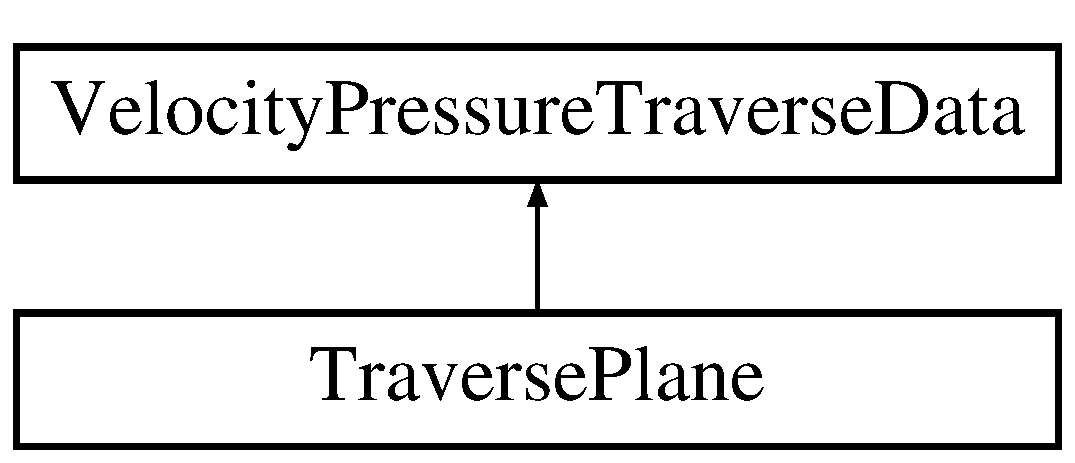
\includegraphics[height=1.924399cm]{d8/d09/class_velocity_pressure_traverse_data}
\end{center}
\end{figure}
\subsection*{Public Member Functions}
\begin{DoxyCompactItemize}
\item 
\mbox{\Hypertarget{class_velocity_pressure_traverse_data_ad40651783106845a732537b60877c70f}\label{class_velocity_pressure_traverse_data_ad40651783106845a732537b60877c70f}} 
double {\bfseries get\+Pv3\+Value} () const
\item 
\mbox{\Hypertarget{class_velocity_pressure_traverse_data_aabde4db04d805c4264d3fc2036ef38a8}\label{class_velocity_pressure_traverse_data_aabde4db04d805c4264d3fc2036ef38a8}} 
double {\bfseries get75percent\+Rule} () const
\item 
\mbox{\Hypertarget{class_velocity_pressure_traverse_data_ad40651783106845a732537b60877c70f}\label{class_velocity_pressure_traverse_data_ad40651783106845a732537b60877c70f}} 
double {\bfseries get\+Pv3\+Value} () const
\item 
\mbox{\Hypertarget{class_velocity_pressure_traverse_data_aabde4db04d805c4264d3fc2036ef38a8}\label{class_velocity_pressure_traverse_data_aabde4db04d805c4264d3fc2036ef38a8}} 
double {\bfseries get75percent\+Rule} () const
\item 
\mbox{\Hypertarget{class_velocity_pressure_traverse_data_ad40651783106845a732537b60877c70f}\label{class_velocity_pressure_traverse_data_ad40651783106845a732537b60877c70f}} 
double {\bfseries get\+Pv3\+Value} () const
\item 
\mbox{\Hypertarget{class_velocity_pressure_traverse_data_aabde4db04d805c4264d3fc2036ef38a8}\label{class_velocity_pressure_traverse_data_aabde4db04d805c4264d3fc2036ef38a8}} 
double {\bfseries get75percent\+Rule} () const
\end{DoxyCompactItemize}
\subsection*{Protected Member Functions}
\begin{DoxyCompactItemize}
\item 
\mbox{\Hypertarget{class_velocity_pressure_traverse_data_a7b099c4eb6b034b880aa167d98848c53}\label{class_velocity_pressure_traverse_data_a7b099c4eb6b034b880aa167d98848c53}} 
{\bfseries Velocity\+Pressure\+Traverse\+Data} (const double pitot\+Tube\+Coefficient, std\+::vector$<$ std\+::vector$<$ double $>$ $>$ traverse\+Hole\+Data)
\item 
\mbox{\Hypertarget{class_velocity_pressure_traverse_data_a7b099c4eb6b034b880aa167d98848c53}\label{class_velocity_pressure_traverse_data_a7b099c4eb6b034b880aa167d98848c53}} 
{\bfseries Velocity\+Pressure\+Traverse\+Data} (const double pitot\+Tube\+Coefficient, std\+::vector$<$ std\+::vector$<$ double $>$ $>$ traverse\+Hole\+Data)
\item 
\mbox{\Hypertarget{class_velocity_pressure_traverse_data_a7b099c4eb6b034b880aa167d98848c53}\label{class_velocity_pressure_traverse_data_a7b099c4eb6b034b880aa167d98848c53}} 
{\bfseries Velocity\+Pressure\+Traverse\+Data} (const double pitot\+Tube\+Coefficient, std\+::vector$<$ std\+::vector$<$ double $>$ $>$ traverse\+Hole\+Data)
\end{DoxyCompactItemize}
\subsection*{Protected Attributes}
\begin{DoxyCompactItemize}
\item 
\mbox{\Hypertarget{class_velocity_pressure_traverse_data_a5f0d183ca647bc7eef7f7c7a44a9c23e}\label{class_velocity_pressure_traverse_data_a5f0d183ca647bc7eef7f7c7a44a9c23e}} 
const double {\bfseries pitot\+Tube\+Coefficient}
\item 
\mbox{\Hypertarget{class_velocity_pressure_traverse_data_ae8ed6cb6fa7aeec774383671c38bc21b}\label{class_velocity_pressure_traverse_data_ae8ed6cb6fa7aeec774383671c38bc21b}} 
double {\bfseries pv3} = 0
\item 
\mbox{\Hypertarget{class_velocity_pressure_traverse_data_aaae013760883326c1c15bc0e2a27cd34}\label{class_velocity_pressure_traverse_data_aaae013760883326c1c15bc0e2a27cd34}} 
double {\bfseries percent75\+Rule} = 0
\item 
\mbox{\Hypertarget{class_velocity_pressure_traverse_data_a02b06c3211e4fb15fdba68127a9855a8}\label{class_velocity_pressure_traverse_data_a02b06c3211e4fb15fdba68127a9855a8}} 
std\+::vector$<$ std\+::vector$<$ double $>$ $>$ {\bfseries traverse\+Hole\+Data}
\end{DoxyCompactItemize}
\subsection*{Friends}
\begin{DoxyCompactItemize}
\item 
\mbox{\Hypertarget{class_velocity_pressure_traverse_data_a31f6bbdce0894df6a817f493afffda84}\label{class_velocity_pressure_traverse_data_a31f6bbdce0894df6a817f493afffda84}} 
class {\bfseries Plane\+Data}
\end{DoxyCompactItemize}


\subsection{Detailed Description}


Definition at line 8 of file Planar.\+h.



The documentation for this class was generated from the following file\+:\begin{DoxyCompactItemize}
\item 
\+\_\+\+C\+Pack\+\_\+\+Packages/\+Darwin/\+S\+T\+G\+Z/amo\+\_\+tools\+\_\+suite-\/-\/\+Darwin-\/x86\+\_\+64-\/\+Debug/amo\+\_\+tools\+\_\+suite/include/fans/Planar.\+h\end{DoxyCompactItemize}

\hypertarget{class_wall_losses}{}\section{Wall\+Losses Class Reference}
\label{class_wall_losses}\index{Wall\+Losses@{Wall\+Losses}}


{\ttfamily \#include $<$Wall\+Losses.\+h$>$}

\subsection*{Public Member Functions}
\begin{DoxyCompactItemize}
\item 
\hyperlink{class_wall_losses_a7d46f259c632ecdcde5ae31468c03e2e}{Wall\+Losses} (const double surface\+Area, const double ambient\+Temperature, const double surface\+Temperature, const double wind\+Velocity, const double surface\+Emissivity, const double condition\+Factor, const double correction\+Factor)
\item 
double \hyperlink{class_wall_losses_ad4d3aa549cc7ab19e927823dbafed973}{get\+Surface\+Area} () const
\item 
void \hyperlink{class_wall_losses_acbbbe4b1ec44bb04e5e1db944017995c}{set\+Surface\+Area} (const double surface\+Area)
\item 
double \hyperlink{class_wall_losses_a806cb5860fe78d0379e3877f043655ad}{get\+Ambient\+Temperature} () const
\item 
void \hyperlink{class_wall_losses_a08a8f4c9add0ce78733be4558cc8410b}{set\+Ambient\+Temperature} (const double ambient\+Temperature)
\item 
double \hyperlink{class_wall_losses_ac2ce3cea6eef435a5fcf6a659b8e7d70}{get\+Surface\+Temperature} () const
\item 
void \hyperlink{class_wall_losses_a7aaa1bd0d7e0ec67db33668ccc6c48da}{set\+Surface\+Temperature} (const double surface\+Temperature)
\item 
double \hyperlink{class_wall_losses_ae68657cacdfbaf8cdc48324dd580cf3b}{get\+Wind\+Velocity} () const
\item 
void \hyperlink{class_wall_losses_ae376b7ce4e5b3c45a663395802c176a9}{set\+Wind\+Velocity} (const double wind\+Velocity)
\item 
double \hyperlink{class_wall_losses_ae1fce9523d14831ef6bc9b7823d5ea08}{get\+Surface\+Emissivity} () const
\item 
void \hyperlink{class_wall_losses_ad0ebd1a0a1b32a2358da15b6c8e63d3a}{set\+Surface\+Emissivity} (const double surface\+Emissivity)
\item 
double \hyperlink{class_wall_losses_a16ab4003a17f9e95f28b9390b92c2b27}{get\+Condition\+Factor} () const
\item 
void \hyperlink{class_wall_losses_a1533a7513460d22f433fb670700573a2}{set\+Condition\+Factor} (const double condition\+Factor)
\item 
double \hyperlink{class_wall_losses_a4ce6a0ec36cd868b14b041f18251cb6d}{get\+Correction\+Factor} () const
\item 
void \hyperlink{class_wall_losses_affdf3f6c3d54d73c7f91e1515fb12533}{set\+Correction\+Factor} (const double correction\+Factor)
\item 
double \hyperlink{class_wall_losses_a884da3507498878f619cbe5ba340c0ef}{get\+Heat\+Loss} ()
\item 
std\+::string \hyperlink{class_wall_losses_a10f5de20dc6fead726adbf62a9c49b09}{get\+Surface} () const
\item 
void \hyperlink{class_wall_losses_af329a27b78e1f2d84af6a48ffc59bfad}{set\+Surface} (std\+::string surface)
\item 
double \hyperlink{class_wall_losses_ad67b46094ba89cb759ec124c63c137de}{get\+ID} () const
\item 
void \hyperlink{class_wall_losses_a91526efc0eb1bf030ebc1d864a21acdd}{set\+ID} (const size\+\_\+t id)
\item 
\mbox{\Hypertarget{class_wall_losses_ad9eebb34927690332c00df51507878e9}\label{class_wall_losses_ad9eebb34927690332c00df51507878e9}} 
bool \hyperlink{class_wall_losses_ad9eebb34927690332c00df51507878e9}{operator==} (const \hyperlink{class_wall_losses}{Wall\+Losses} \&rhs) const
\begin{DoxyCompactList}\small\item\em bool operator \end{DoxyCompactList}\item 
\mbox{\Hypertarget{class_wall_losses_a46d50205e67870978292c4bfa1c9d329}\label{class_wall_losses_a46d50205e67870978292c4bfa1c9d329}} 
bool \hyperlink{class_wall_losses_a46d50205e67870978292c4bfa1c9d329}{operator!=} (const \hyperlink{class_wall_losses}{Wall\+Losses} \&rhs) const
\begin{DoxyCompactList}\small\item\em bool operator \end{DoxyCompactList}\item 
\hyperlink{class_wall_losses_a7d46f259c632ecdcde5ae31468c03e2e}{Wall\+Losses} (const double surface\+Area, const double ambient\+Temperature, const double surface\+Temperature, const double wind\+Velocity, const double surface\+Emissivity, const double condition\+Factor, const double correction\+Factor)
\item 
double \hyperlink{class_wall_losses_ad4d3aa549cc7ab19e927823dbafed973}{get\+Surface\+Area} () const
\item 
void \hyperlink{class_wall_losses_acbbbe4b1ec44bb04e5e1db944017995c}{set\+Surface\+Area} (const double surface\+Area)
\item 
double \hyperlink{class_wall_losses_a806cb5860fe78d0379e3877f043655ad}{get\+Ambient\+Temperature} () const
\item 
void \hyperlink{class_wall_losses_a08a8f4c9add0ce78733be4558cc8410b}{set\+Ambient\+Temperature} (const double ambient\+Temperature)
\item 
double \hyperlink{class_wall_losses_ac2ce3cea6eef435a5fcf6a659b8e7d70}{get\+Surface\+Temperature} () const
\item 
void \hyperlink{class_wall_losses_a7aaa1bd0d7e0ec67db33668ccc6c48da}{set\+Surface\+Temperature} (const double surface\+Temperature)
\item 
double \hyperlink{class_wall_losses_ae68657cacdfbaf8cdc48324dd580cf3b}{get\+Wind\+Velocity} () const
\item 
void \hyperlink{class_wall_losses_ae376b7ce4e5b3c45a663395802c176a9}{set\+Wind\+Velocity} (const double wind\+Velocity)
\item 
double \hyperlink{class_wall_losses_ae1fce9523d14831ef6bc9b7823d5ea08}{get\+Surface\+Emissivity} () const
\item 
void \hyperlink{class_wall_losses_ad0ebd1a0a1b32a2358da15b6c8e63d3a}{set\+Surface\+Emissivity} (const double surface\+Emissivity)
\item 
double \hyperlink{class_wall_losses_a16ab4003a17f9e95f28b9390b92c2b27}{get\+Condition\+Factor} () const
\item 
void \hyperlink{class_wall_losses_a1533a7513460d22f433fb670700573a2}{set\+Condition\+Factor} (const double condition\+Factor)
\item 
double \hyperlink{class_wall_losses_a4ce6a0ec36cd868b14b041f18251cb6d}{get\+Correction\+Factor} () const
\item 
void \hyperlink{class_wall_losses_affdf3f6c3d54d73c7f91e1515fb12533}{set\+Correction\+Factor} (const double correction\+Factor)
\item 
double \hyperlink{class_wall_losses_a884da3507498878f619cbe5ba340c0ef}{get\+Heat\+Loss} ()
\item 
std\+::string \hyperlink{class_wall_losses_a10f5de20dc6fead726adbf62a9c49b09}{get\+Surface} () const
\item 
void \hyperlink{class_wall_losses_af329a27b78e1f2d84af6a48ffc59bfad}{set\+Surface} (std\+::string surface)
\item 
double \hyperlink{class_wall_losses_ad67b46094ba89cb759ec124c63c137de}{get\+ID} () const
\item 
void \hyperlink{class_wall_losses_a91526efc0eb1bf030ebc1d864a21acdd}{set\+ID} (const size\+\_\+t id)
\item 
\mbox{\Hypertarget{class_wall_losses_ad9eebb34927690332c00df51507878e9}\label{class_wall_losses_ad9eebb34927690332c00df51507878e9}} 
bool \hyperlink{class_wall_losses_ad9eebb34927690332c00df51507878e9}{operator==} (const \hyperlink{class_wall_losses}{Wall\+Losses} \&rhs) const
\begin{DoxyCompactList}\small\item\em bool operator \end{DoxyCompactList}\item 
\mbox{\Hypertarget{class_wall_losses_a46d50205e67870978292c4bfa1c9d329}\label{class_wall_losses_a46d50205e67870978292c4bfa1c9d329}} 
bool \hyperlink{class_wall_losses_a46d50205e67870978292c4bfa1c9d329}{operator!=} (const \hyperlink{class_wall_losses}{Wall\+Losses} \&rhs) const
\begin{DoxyCompactList}\small\item\em bool operator \end{DoxyCompactList}\item 
\hyperlink{class_wall_losses_a7d46f259c632ecdcde5ae31468c03e2e}{Wall\+Losses} (const double surface\+Area, const double ambient\+Temperature, const double surface\+Temperature, const double wind\+Velocity, const double surface\+Emissivity, const double condition\+Factor, const double correction\+Factor)
\item 
double \hyperlink{class_wall_losses_ad4d3aa549cc7ab19e927823dbafed973}{get\+Surface\+Area} () const
\item 
void \hyperlink{class_wall_losses_acbbbe4b1ec44bb04e5e1db944017995c}{set\+Surface\+Area} (const double surface\+Area)
\item 
double \hyperlink{class_wall_losses_a806cb5860fe78d0379e3877f043655ad}{get\+Ambient\+Temperature} () const
\item 
void \hyperlink{class_wall_losses_a08a8f4c9add0ce78733be4558cc8410b}{set\+Ambient\+Temperature} (const double ambient\+Temperature)
\item 
double \hyperlink{class_wall_losses_ac2ce3cea6eef435a5fcf6a659b8e7d70}{get\+Surface\+Temperature} () const
\item 
void \hyperlink{class_wall_losses_a7aaa1bd0d7e0ec67db33668ccc6c48da}{set\+Surface\+Temperature} (const double surface\+Temperature)
\item 
double \hyperlink{class_wall_losses_ae68657cacdfbaf8cdc48324dd580cf3b}{get\+Wind\+Velocity} () const
\item 
void \hyperlink{class_wall_losses_ae376b7ce4e5b3c45a663395802c176a9}{set\+Wind\+Velocity} (const double wind\+Velocity)
\item 
double \hyperlink{class_wall_losses_ae1fce9523d14831ef6bc9b7823d5ea08}{get\+Surface\+Emissivity} () const
\item 
void \hyperlink{class_wall_losses_ad0ebd1a0a1b32a2358da15b6c8e63d3a}{set\+Surface\+Emissivity} (const double surface\+Emissivity)
\item 
double \hyperlink{class_wall_losses_a16ab4003a17f9e95f28b9390b92c2b27}{get\+Condition\+Factor} () const
\item 
void \hyperlink{class_wall_losses_a1533a7513460d22f433fb670700573a2}{set\+Condition\+Factor} (const double condition\+Factor)
\item 
double \hyperlink{class_wall_losses_a4ce6a0ec36cd868b14b041f18251cb6d}{get\+Correction\+Factor} () const
\item 
void \hyperlink{class_wall_losses_affdf3f6c3d54d73c7f91e1515fb12533}{set\+Correction\+Factor} (const double correction\+Factor)
\item 
double \hyperlink{class_wall_losses_a884da3507498878f619cbe5ba340c0ef}{get\+Heat\+Loss} ()
\item 
std\+::string \hyperlink{class_wall_losses_a10f5de20dc6fead726adbf62a9c49b09}{get\+Surface} () const
\item 
void \hyperlink{class_wall_losses_af329a27b78e1f2d84af6a48ffc59bfad}{set\+Surface} (std\+::string surface)
\item 
double \hyperlink{class_wall_losses_ad67b46094ba89cb759ec124c63c137de}{get\+ID} () const
\item 
void \hyperlink{class_wall_losses_a91526efc0eb1bf030ebc1d864a21acdd}{set\+ID} (const size\+\_\+t id)
\item 
\mbox{\Hypertarget{class_wall_losses_ad9eebb34927690332c00df51507878e9}\label{class_wall_losses_ad9eebb34927690332c00df51507878e9}} 
bool \hyperlink{class_wall_losses_ad9eebb34927690332c00df51507878e9}{operator==} (const \hyperlink{class_wall_losses}{Wall\+Losses} \&rhs) const
\begin{DoxyCompactList}\small\item\em bool operator \end{DoxyCompactList}\item 
\mbox{\Hypertarget{class_wall_losses_a46d50205e67870978292c4bfa1c9d329}\label{class_wall_losses_a46d50205e67870978292c4bfa1c9d329}} 
bool \hyperlink{class_wall_losses_a46d50205e67870978292c4bfa1c9d329}{operator!=} (const \hyperlink{class_wall_losses}{Wall\+Losses} \&rhs) const
\begin{DoxyCompactList}\small\item\em bool operator \end{DoxyCompactList}\end{DoxyCompactItemize}
\subsection*{Friends}
\begin{DoxyCompactItemize}
\item 
\mbox{\Hypertarget{class_wall_losses_a0102f3b3c0cbf96db6c49f071fa5e7cc}\label{class_wall_losses_a0102f3b3c0cbf96db6c49f071fa5e7cc}} 
class {\bfseries S\+Q\+Lite}
\end{DoxyCompactItemize}


\subsection{Detailed Description}
Wall Losses class Contains all of the properties of a wall loss Used to calculate the heat loss caused by heat being transferred from the outer surface of the wall to the surroundings. A\+S\+S\+U\+M\+P\+T\+I\+O\+NS\+: Surface emissivity is uniform for the entire surface area. Wind velocity is uniform over the entire surface area. 

Definition at line 28 of file Wall\+Losses.\+h.



\subsection{Constructor \& Destructor Documentation}
\mbox{\Hypertarget{class_wall_losses_a7d46f259c632ecdcde5ae31468c03e2e}\label{class_wall_losses_a7d46f259c632ecdcde5ae31468c03e2e}} 
\index{Wall\+Losses@{Wall\+Losses}!Wall\+Losses@{Wall\+Losses}}
\index{Wall\+Losses@{Wall\+Losses}!Wall\+Losses@{Wall\+Losses}}
\subsubsection{\texorpdfstring{Wall\+Losses()}{WallLosses()}\hspace{0.1cm}{\footnotesize\ttfamily [1/3]}}
{\footnotesize\ttfamily Wall\+Losses\+::\+Wall\+Losses (\begin{DoxyParamCaption}\item[{const double}]{surface\+Area,  }\item[{const double}]{ambient\+Temperature,  }\item[{const double}]{surface\+Temperature,  }\item[{const double}]{wind\+Velocity,  }\item[{const double}]{surface\+Emissivity,  }\item[{const double}]{condition\+Factor,  }\item[{const double}]{correction\+Factor }\end{DoxyParamCaption})\hspace{0.3cm}{\ttfamily [inline]}}

Constructor 
\begin{DoxyParams}{Parameters}
{\em surface\+Area} & double, total outside surface area in ft$^\wedge$2 \\
\hline
{\em ambient\+Temperature} & double, ambient temperature in °F \\
\hline
{\em surface\+Temperature} & double, average surface temperature (measured) in °F \\
\hline
{\em wind\+Velocity} & double, wind velocity in miles/hr \\
\hline
{\em surface\+Emissivity} & double, surface emissivity -\/ unitless \\
\hline
{\em condition\+Factor} & double, condition factor -\/ unitless \\
\hline
{\em correction\+Factor} & double, correction factor -\/ unitless \\
\hline
\end{DoxyParams}


Definition at line 41 of file Wall\+Losses.\+h.

\mbox{\Hypertarget{class_wall_losses_a7d46f259c632ecdcde5ae31468c03e2e}\label{class_wall_losses_a7d46f259c632ecdcde5ae31468c03e2e}} 
\index{Wall\+Losses@{Wall\+Losses}!Wall\+Losses@{Wall\+Losses}}
\index{Wall\+Losses@{Wall\+Losses}!Wall\+Losses@{Wall\+Losses}}
\subsubsection{\texorpdfstring{Wall\+Losses()}{WallLosses()}\hspace{0.1cm}{\footnotesize\ttfamily [2/3]}}
{\footnotesize\ttfamily Wall\+Losses\+::\+Wall\+Losses (\begin{DoxyParamCaption}\item[{const double}]{surface\+Area,  }\item[{const double}]{ambient\+Temperature,  }\item[{const double}]{surface\+Temperature,  }\item[{const double}]{wind\+Velocity,  }\item[{const double}]{surface\+Emissivity,  }\item[{const double}]{condition\+Factor,  }\item[{const double}]{correction\+Factor }\end{DoxyParamCaption})\hspace{0.3cm}{\ttfamily [inline]}}

Constructor 
\begin{DoxyParams}{Parameters}
{\em surface\+Area} & double, total outside surface area in ft$^\wedge$2 \\
\hline
{\em ambient\+Temperature} & double, ambient temperature in °F \\
\hline
{\em surface\+Temperature} & double, average surface temperature (measured) in °F \\
\hline
{\em wind\+Velocity} & double, wind velocity in miles/hr \\
\hline
{\em surface\+Emissivity} & double, surface emissivity -\/ unitless \\
\hline
{\em condition\+Factor} & double, condition factor -\/ unitless \\
\hline
{\em correction\+Factor} & double, correction factor -\/ unitless \\
\hline
\end{DoxyParams}


Definition at line 41 of file Wall\+Losses.\+h.

\mbox{\Hypertarget{class_wall_losses_a7d46f259c632ecdcde5ae31468c03e2e}\label{class_wall_losses_a7d46f259c632ecdcde5ae31468c03e2e}} 
\index{Wall\+Losses@{Wall\+Losses}!Wall\+Losses@{Wall\+Losses}}
\index{Wall\+Losses@{Wall\+Losses}!Wall\+Losses@{Wall\+Losses}}
\subsubsection{\texorpdfstring{Wall\+Losses()}{WallLosses()}\hspace{0.1cm}{\footnotesize\ttfamily [3/3]}}
{\footnotesize\ttfamily Wall\+Losses\+::\+Wall\+Losses (\begin{DoxyParamCaption}\item[{const double}]{surface\+Area,  }\item[{const double}]{ambient\+Temperature,  }\item[{const double}]{surface\+Temperature,  }\item[{const double}]{wind\+Velocity,  }\item[{const double}]{surface\+Emissivity,  }\item[{const double}]{condition\+Factor,  }\item[{const double}]{correction\+Factor }\end{DoxyParamCaption})\hspace{0.3cm}{\ttfamily [inline]}}

Constructor 
\begin{DoxyParams}{Parameters}
{\em surface\+Area} & double, total outside surface area in ft$^\wedge$2 \\
\hline
{\em ambient\+Temperature} & double, ambient temperature in °F \\
\hline
{\em surface\+Temperature} & double, average surface temperature (measured) in °F \\
\hline
{\em wind\+Velocity} & double, wind velocity in miles/hr \\
\hline
{\em surface\+Emissivity} & double, surface emissivity -\/ unitless \\
\hline
{\em condition\+Factor} & double, condition factor -\/ unitless \\
\hline
{\em correction\+Factor} & double, correction factor -\/ unitless \\
\hline
\end{DoxyParams}


Definition at line 41 of file Wall\+Losses.\+h.



\subsection{Member Function Documentation}
\mbox{\Hypertarget{class_wall_losses_a806cb5860fe78d0379e3877f043655ad}\label{class_wall_losses_a806cb5860fe78d0379e3877f043655ad}} 
\index{Wall\+Losses@{Wall\+Losses}!get\+Ambient\+Temperature@{get\+Ambient\+Temperature}}
\index{get\+Ambient\+Temperature@{get\+Ambient\+Temperature}!Wall\+Losses@{Wall\+Losses}}
\subsubsection{\texorpdfstring{get\+Ambient\+Temperature()}{getAmbientTemperature()}\hspace{0.1cm}{\footnotesize\ttfamily [1/3]}}
{\footnotesize\ttfamily double Wall\+Losses\+::get\+Ambient\+Temperature (\begin{DoxyParamCaption}{ }\end{DoxyParamCaption}) const\hspace{0.3cm}{\ttfamily [inline]}}

Gets the ambient temperature \begin{DoxyReturn}{Returns}
double, ambient temperature in °F 
\end{DoxyReturn}


Definition at line 77 of file Wall\+Losses.\+h.

\mbox{\Hypertarget{class_wall_losses_a806cb5860fe78d0379e3877f043655ad}\label{class_wall_losses_a806cb5860fe78d0379e3877f043655ad}} 
\index{Wall\+Losses@{Wall\+Losses}!get\+Ambient\+Temperature@{get\+Ambient\+Temperature}}
\index{get\+Ambient\+Temperature@{get\+Ambient\+Temperature}!Wall\+Losses@{Wall\+Losses}}
\subsubsection{\texorpdfstring{get\+Ambient\+Temperature()}{getAmbientTemperature()}\hspace{0.1cm}{\footnotesize\ttfamily [2/3]}}
{\footnotesize\ttfamily double Wall\+Losses\+::get\+Ambient\+Temperature (\begin{DoxyParamCaption}{ }\end{DoxyParamCaption}) const\hspace{0.3cm}{\ttfamily [inline]}}

Gets the ambient temperature \begin{DoxyReturn}{Returns}
double, ambient temperature in °F 
\end{DoxyReturn}


Definition at line 77 of file Wall\+Losses.\+h.

\mbox{\Hypertarget{class_wall_losses_a806cb5860fe78d0379e3877f043655ad}\label{class_wall_losses_a806cb5860fe78d0379e3877f043655ad}} 
\index{Wall\+Losses@{Wall\+Losses}!get\+Ambient\+Temperature@{get\+Ambient\+Temperature}}
\index{get\+Ambient\+Temperature@{get\+Ambient\+Temperature}!Wall\+Losses@{Wall\+Losses}}
\subsubsection{\texorpdfstring{get\+Ambient\+Temperature()}{getAmbientTemperature()}\hspace{0.1cm}{\footnotesize\ttfamily [3/3]}}
{\footnotesize\ttfamily double Wall\+Losses\+::get\+Ambient\+Temperature (\begin{DoxyParamCaption}{ }\end{DoxyParamCaption}) const\hspace{0.3cm}{\ttfamily [inline]}}

Gets the ambient temperature \begin{DoxyReturn}{Returns}
double, ambient temperature in °F 
\end{DoxyReturn}


Definition at line 77 of file Wall\+Losses.\+h.

\mbox{\Hypertarget{class_wall_losses_a16ab4003a17f9e95f28b9390b92c2b27}\label{class_wall_losses_a16ab4003a17f9e95f28b9390b92c2b27}} 
\index{Wall\+Losses@{Wall\+Losses}!get\+Condition\+Factor@{get\+Condition\+Factor}}
\index{get\+Condition\+Factor@{get\+Condition\+Factor}!Wall\+Losses@{Wall\+Losses}}
\subsubsection{\texorpdfstring{get\+Condition\+Factor()}{getConditionFactor()}\hspace{0.1cm}{\footnotesize\ttfamily [1/3]}}
{\footnotesize\ttfamily double Wall\+Losses\+::get\+Condition\+Factor (\begin{DoxyParamCaption}{ }\end{DoxyParamCaption}) const\hspace{0.3cm}{\ttfamily [inline]}}

Gets the condition factor. The condition factor is the surface shape/orientation factor. \begin{DoxyReturn}{Returns}
double, condition factor 
\end{DoxyReturn}


Definition at line 141 of file Wall\+Losses.\+h.

\mbox{\Hypertarget{class_wall_losses_a16ab4003a17f9e95f28b9390b92c2b27}\label{class_wall_losses_a16ab4003a17f9e95f28b9390b92c2b27}} 
\index{Wall\+Losses@{Wall\+Losses}!get\+Condition\+Factor@{get\+Condition\+Factor}}
\index{get\+Condition\+Factor@{get\+Condition\+Factor}!Wall\+Losses@{Wall\+Losses}}
\subsubsection{\texorpdfstring{get\+Condition\+Factor()}{getConditionFactor()}\hspace{0.1cm}{\footnotesize\ttfamily [2/3]}}
{\footnotesize\ttfamily double Wall\+Losses\+::get\+Condition\+Factor (\begin{DoxyParamCaption}{ }\end{DoxyParamCaption}) const\hspace{0.3cm}{\ttfamily [inline]}}

Gets the condition factor. The condition factor is the surface shape/orientation factor. \begin{DoxyReturn}{Returns}
double, condition factor 
\end{DoxyReturn}


Definition at line 141 of file Wall\+Losses.\+h.

\mbox{\Hypertarget{class_wall_losses_a16ab4003a17f9e95f28b9390b92c2b27}\label{class_wall_losses_a16ab4003a17f9e95f28b9390b92c2b27}} 
\index{Wall\+Losses@{Wall\+Losses}!get\+Condition\+Factor@{get\+Condition\+Factor}}
\index{get\+Condition\+Factor@{get\+Condition\+Factor}!Wall\+Losses@{Wall\+Losses}}
\subsubsection{\texorpdfstring{get\+Condition\+Factor()}{getConditionFactor()}\hspace{0.1cm}{\footnotesize\ttfamily [3/3]}}
{\footnotesize\ttfamily double Wall\+Losses\+::get\+Condition\+Factor (\begin{DoxyParamCaption}{ }\end{DoxyParamCaption}) const\hspace{0.3cm}{\ttfamily [inline]}}

Gets the condition factor. The condition factor is the surface shape/orientation factor. \begin{DoxyReturn}{Returns}
double, condition factor 
\end{DoxyReturn}


Definition at line 141 of file Wall\+Losses.\+h.

\mbox{\Hypertarget{class_wall_losses_a4ce6a0ec36cd868b14b041f18251cb6d}\label{class_wall_losses_a4ce6a0ec36cd868b14b041f18251cb6d}} 
\index{Wall\+Losses@{Wall\+Losses}!get\+Correction\+Factor@{get\+Correction\+Factor}}
\index{get\+Correction\+Factor@{get\+Correction\+Factor}!Wall\+Losses@{Wall\+Losses}}
\subsubsection{\texorpdfstring{get\+Correction\+Factor()}{getCorrectionFactor()}\hspace{0.1cm}{\footnotesize\ttfamily [1/3]}}
{\footnotesize\ttfamily double Wall\+Losses\+::get\+Correction\+Factor (\begin{DoxyParamCaption}{ }\end{DoxyParamCaption}) const\hspace{0.3cm}{\ttfamily [inline]}}

Gets the correction factor \begin{DoxyReturn}{Returns}
double, correction factor -\/ unitless 
\end{DoxyReturn}


Definition at line 157 of file Wall\+Losses.\+h.

\mbox{\Hypertarget{class_wall_losses_a4ce6a0ec36cd868b14b041f18251cb6d}\label{class_wall_losses_a4ce6a0ec36cd868b14b041f18251cb6d}} 
\index{Wall\+Losses@{Wall\+Losses}!get\+Correction\+Factor@{get\+Correction\+Factor}}
\index{get\+Correction\+Factor@{get\+Correction\+Factor}!Wall\+Losses@{Wall\+Losses}}
\subsubsection{\texorpdfstring{get\+Correction\+Factor()}{getCorrectionFactor()}\hspace{0.1cm}{\footnotesize\ttfamily [2/3]}}
{\footnotesize\ttfamily double Wall\+Losses\+::get\+Correction\+Factor (\begin{DoxyParamCaption}{ }\end{DoxyParamCaption}) const\hspace{0.3cm}{\ttfamily [inline]}}

Gets the correction factor \begin{DoxyReturn}{Returns}
double, correction factor -\/ unitless 
\end{DoxyReturn}


Definition at line 157 of file Wall\+Losses.\+h.

\mbox{\Hypertarget{class_wall_losses_a4ce6a0ec36cd868b14b041f18251cb6d}\label{class_wall_losses_a4ce6a0ec36cd868b14b041f18251cb6d}} 
\index{Wall\+Losses@{Wall\+Losses}!get\+Correction\+Factor@{get\+Correction\+Factor}}
\index{get\+Correction\+Factor@{get\+Correction\+Factor}!Wall\+Losses@{Wall\+Losses}}
\subsubsection{\texorpdfstring{get\+Correction\+Factor()}{getCorrectionFactor()}\hspace{0.1cm}{\footnotesize\ttfamily [3/3]}}
{\footnotesize\ttfamily double Wall\+Losses\+::get\+Correction\+Factor (\begin{DoxyParamCaption}{ }\end{DoxyParamCaption}) const\hspace{0.3cm}{\ttfamily [inline]}}

Gets the correction factor \begin{DoxyReturn}{Returns}
double, correction factor -\/ unitless 
\end{DoxyReturn}


Definition at line 157 of file Wall\+Losses.\+h.

\mbox{\Hypertarget{class_wall_losses_a884da3507498878f619cbe5ba340c0ef}\label{class_wall_losses_a884da3507498878f619cbe5ba340c0ef}} 
\index{Wall\+Losses@{Wall\+Losses}!get\+Heat\+Loss@{get\+Heat\+Loss}}
\index{get\+Heat\+Loss@{get\+Heat\+Loss}!Wall\+Losses@{Wall\+Losses}}
\subsubsection{\texorpdfstring{get\+Heat\+Loss()}{getHeatLoss()}\hspace{0.1cm}{\footnotesize\ttfamily [1/3]}}
{\footnotesize\ttfamily double Wall\+Losses\+::get\+Heat\+Loss (\begin{DoxyParamCaption}{ }\end{DoxyParamCaption})}

Calculates the wall heat loss \begin{DoxyReturn}{Returns}
double, wall heat loss in btu/hr 
\end{DoxyReturn}
\mbox{\Hypertarget{class_wall_losses_a884da3507498878f619cbe5ba340c0ef}\label{class_wall_losses_a884da3507498878f619cbe5ba340c0ef}} 
\index{Wall\+Losses@{Wall\+Losses}!get\+Heat\+Loss@{get\+Heat\+Loss}}
\index{get\+Heat\+Loss@{get\+Heat\+Loss}!Wall\+Losses@{Wall\+Losses}}
\subsubsection{\texorpdfstring{get\+Heat\+Loss()}{getHeatLoss()}\hspace{0.1cm}{\footnotesize\ttfamily [2/3]}}
{\footnotesize\ttfamily double Wall\+Losses\+::get\+Heat\+Loss (\begin{DoxyParamCaption}{ }\end{DoxyParamCaption})}

Calculates the wall heat loss \begin{DoxyReturn}{Returns}
double, wall heat loss in btu/hr 
\end{DoxyReturn}


Definition at line 12 of file Wall\+Losses.\+cpp.

\mbox{\Hypertarget{class_wall_losses_a884da3507498878f619cbe5ba340c0ef}\label{class_wall_losses_a884da3507498878f619cbe5ba340c0ef}} 
\index{Wall\+Losses@{Wall\+Losses}!get\+Heat\+Loss@{get\+Heat\+Loss}}
\index{get\+Heat\+Loss@{get\+Heat\+Loss}!Wall\+Losses@{Wall\+Losses}}
\subsubsection{\texorpdfstring{get\+Heat\+Loss()}{getHeatLoss()}\hspace{0.1cm}{\footnotesize\ttfamily [3/3]}}
{\footnotesize\ttfamily double Wall\+Losses\+::get\+Heat\+Loss (\begin{DoxyParamCaption}{ }\end{DoxyParamCaption})}

Calculates the wall heat loss \begin{DoxyReturn}{Returns}
double, wall heat loss in btu/hr 
\end{DoxyReturn}
\mbox{\Hypertarget{class_wall_losses_ad67b46094ba89cb759ec124c63c137de}\label{class_wall_losses_ad67b46094ba89cb759ec124c63c137de}} 
\index{Wall\+Losses@{Wall\+Losses}!get\+ID@{get\+ID}}
\index{get\+ID@{get\+ID}!Wall\+Losses@{Wall\+Losses}}
\subsubsection{\texorpdfstring{get\+I\+D()}{getID()}\hspace{0.1cm}{\footnotesize\ttfamily [1/3]}}
{\footnotesize\ttfamily double Wall\+Losses\+::get\+ID (\begin{DoxyParamCaption}{ }\end{DoxyParamCaption}) const\hspace{0.3cm}{\ttfamily [inline]}}

Gets the ID of surface description \begin{DoxyReturn}{Returns}
double, ID of surface description 
\end{DoxyReturn}


Definition at line 195 of file Wall\+Losses.\+h.

\mbox{\Hypertarget{class_wall_losses_ad67b46094ba89cb759ec124c63c137de}\label{class_wall_losses_ad67b46094ba89cb759ec124c63c137de}} 
\index{Wall\+Losses@{Wall\+Losses}!get\+ID@{get\+ID}}
\index{get\+ID@{get\+ID}!Wall\+Losses@{Wall\+Losses}}
\subsubsection{\texorpdfstring{get\+I\+D()}{getID()}\hspace{0.1cm}{\footnotesize\ttfamily [2/3]}}
{\footnotesize\ttfamily double Wall\+Losses\+::get\+ID (\begin{DoxyParamCaption}{ }\end{DoxyParamCaption}) const\hspace{0.3cm}{\ttfamily [inline]}}

Gets the ID of surface description \begin{DoxyReturn}{Returns}
double, ID of surface description 
\end{DoxyReturn}


Definition at line 195 of file Wall\+Losses.\+h.

\mbox{\Hypertarget{class_wall_losses_ad67b46094ba89cb759ec124c63c137de}\label{class_wall_losses_ad67b46094ba89cb759ec124c63c137de}} 
\index{Wall\+Losses@{Wall\+Losses}!get\+ID@{get\+ID}}
\index{get\+ID@{get\+ID}!Wall\+Losses@{Wall\+Losses}}
\subsubsection{\texorpdfstring{get\+I\+D()}{getID()}\hspace{0.1cm}{\footnotesize\ttfamily [3/3]}}
{\footnotesize\ttfamily double Wall\+Losses\+::get\+ID (\begin{DoxyParamCaption}{ }\end{DoxyParamCaption}) const\hspace{0.3cm}{\ttfamily [inline]}}

Gets the ID of surface description \begin{DoxyReturn}{Returns}
double, ID of surface description 
\end{DoxyReturn}


Definition at line 195 of file Wall\+Losses.\+h.

\mbox{\Hypertarget{class_wall_losses_a10f5de20dc6fead726adbf62a9c49b09}\label{class_wall_losses_a10f5de20dc6fead726adbf62a9c49b09}} 
\index{Wall\+Losses@{Wall\+Losses}!get\+Surface@{get\+Surface}}
\index{get\+Surface@{get\+Surface}!Wall\+Losses@{Wall\+Losses}}
\subsubsection{\texorpdfstring{get\+Surface()}{getSurface()}\hspace{0.1cm}{\footnotesize\ttfamily [1/3]}}
{\footnotesize\ttfamily std\+::string Wall\+Losses\+::get\+Surface (\begin{DoxyParamCaption}{ }\end{DoxyParamCaption}) const\hspace{0.3cm}{\ttfamily [inline]}}

Gets the surface description \begin{DoxyReturn}{Returns}
string, surface description 
\end{DoxyReturn}


Definition at line 179 of file Wall\+Losses.\+h.

\mbox{\Hypertarget{class_wall_losses_a10f5de20dc6fead726adbf62a9c49b09}\label{class_wall_losses_a10f5de20dc6fead726adbf62a9c49b09}} 
\index{Wall\+Losses@{Wall\+Losses}!get\+Surface@{get\+Surface}}
\index{get\+Surface@{get\+Surface}!Wall\+Losses@{Wall\+Losses}}
\subsubsection{\texorpdfstring{get\+Surface()}{getSurface()}\hspace{0.1cm}{\footnotesize\ttfamily [2/3]}}
{\footnotesize\ttfamily std\+::string Wall\+Losses\+::get\+Surface (\begin{DoxyParamCaption}{ }\end{DoxyParamCaption}) const\hspace{0.3cm}{\ttfamily [inline]}}

Gets the surface description \begin{DoxyReturn}{Returns}
string, surface description 
\end{DoxyReturn}


Definition at line 179 of file Wall\+Losses.\+h.

\mbox{\Hypertarget{class_wall_losses_a10f5de20dc6fead726adbf62a9c49b09}\label{class_wall_losses_a10f5de20dc6fead726adbf62a9c49b09}} 
\index{Wall\+Losses@{Wall\+Losses}!get\+Surface@{get\+Surface}}
\index{get\+Surface@{get\+Surface}!Wall\+Losses@{Wall\+Losses}}
\subsubsection{\texorpdfstring{get\+Surface()}{getSurface()}\hspace{0.1cm}{\footnotesize\ttfamily [3/3]}}
{\footnotesize\ttfamily std\+::string Wall\+Losses\+::get\+Surface (\begin{DoxyParamCaption}{ }\end{DoxyParamCaption}) const\hspace{0.3cm}{\ttfamily [inline]}}

Gets the surface description \begin{DoxyReturn}{Returns}
string, surface description 
\end{DoxyReturn}


Definition at line 179 of file Wall\+Losses.\+h.

\mbox{\Hypertarget{class_wall_losses_ad4d3aa549cc7ab19e927823dbafed973}\label{class_wall_losses_ad4d3aa549cc7ab19e927823dbafed973}} 
\index{Wall\+Losses@{Wall\+Losses}!get\+Surface\+Area@{get\+Surface\+Area}}
\index{get\+Surface\+Area@{get\+Surface\+Area}!Wall\+Losses@{Wall\+Losses}}
\subsubsection{\texorpdfstring{get\+Surface\+Area()}{getSurfaceArea()}\hspace{0.1cm}{\footnotesize\ttfamily [1/3]}}
{\footnotesize\ttfamily double Wall\+Losses\+::get\+Surface\+Area (\begin{DoxyParamCaption}{ }\end{DoxyParamCaption}) const\hspace{0.3cm}{\ttfamily [inline]}}

Gets the total outside surface area \begin{DoxyReturn}{Returns}
double, total outside surface area in ft$^\wedge$2 
\end{DoxyReturn}


Definition at line 61 of file Wall\+Losses.\+h.

\mbox{\Hypertarget{class_wall_losses_ad4d3aa549cc7ab19e927823dbafed973}\label{class_wall_losses_ad4d3aa549cc7ab19e927823dbafed973}} 
\index{Wall\+Losses@{Wall\+Losses}!get\+Surface\+Area@{get\+Surface\+Area}}
\index{get\+Surface\+Area@{get\+Surface\+Area}!Wall\+Losses@{Wall\+Losses}}
\subsubsection{\texorpdfstring{get\+Surface\+Area()}{getSurfaceArea()}\hspace{0.1cm}{\footnotesize\ttfamily [2/3]}}
{\footnotesize\ttfamily double Wall\+Losses\+::get\+Surface\+Area (\begin{DoxyParamCaption}{ }\end{DoxyParamCaption}) const\hspace{0.3cm}{\ttfamily [inline]}}

Gets the total outside surface area \begin{DoxyReturn}{Returns}
double, total outside surface area in ft$^\wedge$2 
\end{DoxyReturn}


Definition at line 61 of file Wall\+Losses.\+h.

\mbox{\Hypertarget{class_wall_losses_ad4d3aa549cc7ab19e927823dbafed973}\label{class_wall_losses_ad4d3aa549cc7ab19e927823dbafed973}} 
\index{Wall\+Losses@{Wall\+Losses}!get\+Surface\+Area@{get\+Surface\+Area}}
\index{get\+Surface\+Area@{get\+Surface\+Area}!Wall\+Losses@{Wall\+Losses}}
\subsubsection{\texorpdfstring{get\+Surface\+Area()}{getSurfaceArea()}\hspace{0.1cm}{\footnotesize\ttfamily [3/3]}}
{\footnotesize\ttfamily double Wall\+Losses\+::get\+Surface\+Area (\begin{DoxyParamCaption}{ }\end{DoxyParamCaption}) const\hspace{0.3cm}{\ttfamily [inline]}}

Gets the total outside surface area \begin{DoxyReturn}{Returns}
double, total outside surface area in ft$^\wedge$2 
\end{DoxyReturn}


Definition at line 61 of file Wall\+Losses.\+h.

\mbox{\Hypertarget{class_wall_losses_ae1fce9523d14831ef6bc9b7823d5ea08}\label{class_wall_losses_ae1fce9523d14831ef6bc9b7823d5ea08}} 
\index{Wall\+Losses@{Wall\+Losses}!get\+Surface\+Emissivity@{get\+Surface\+Emissivity}}
\index{get\+Surface\+Emissivity@{get\+Surface\+Emissivity}!Wall\+Losses@{Wall\+Losses}}
\subsubsection{\texorpdfstring{get\+Surface\+Emissivity()}{getSurfaceEmissivity()}\hspace{0.1cm}{\footnotesize\ttfamily [1/3]}}
{\footnotesize\ttfamily double Wall\+Losses\+::get\+Surface\+Emissivity (\begin{DoxyParamCaption}{ }\end{DoxyParamCaption}) const\hspace{0.3cm}{\ttfamily [inline]}}

Gets the surface emissivity (Typical -\/ 0.\+9) \begin{DoxyReturn}{Returns}
double, surface emissivity -\/ unitless 
\end{DoxyReturn}


Definition at line 125 of file Wall\+Losses.\+h.

\mbox{\Hypertarget{class_wall_losses_ae1fce9523d14831ef6bc9b7823d5ea08}\label{class_wall_losses_ae1fce9523d14831ef6bc9b7823d5ea08}} 
\index{Wall\+Losses@{Wall\+Losses}!get\+Surface\+Emissivity@{get\+Surface\+Emissivity}}
\index{get\+Surface\+Emissivity@{get\+Surface\+Emissivity}!Wall\+Losses@{Wall\+Losses}}
\subsubsection{\texorpdfstring{get\+Surface\+Emissivity()}{getSurfaceEmissivity()}\hspace{0.1cm}{\footnotesize\ttfamily [2/3]}}
{\footnotesize\ttfamily double Wall\+Losses\+::get\+Surface\+Emissivity (\begin{DoxyParamCaption}{ }\end{DoxyParamCaption}) const\hspace{0.3cm}{\ttfamily [inline]}}

Gets the surface emissivity (Typical -\/ 0.\+9) \begin{DoxyReturn}{Returns}
double, surface emissivity -\/ unitless 
\end{DoxyReturn}


Definition at line 125 of file Wall\+Losses.\+h.

\mbox{\Hypertarget{class_wall_losses_ae1fce9523d14831ef6bc9b7823d5ea08}\label{class_wall_losses_ae1fce9523d14831ef6bc9b7823d5ea08}} 
\index{Wall\+Losses@{Wall\+Losses}!get\+Surface\+Emissivity@{get\+Surface\+Emissivity}}
\index{get\+Surface\+Emissivity@{get\+Surface\+Emissivity}!Wall\+Losses@{Wall\+Losses}}
\subsubsection{\texorpdfstring{get\+Surface\+Emissivity()}{getSurfaceEmissivity()}\hspace{0.1cm}{\footnotesize\ttfamily [3/3]}}
{\footnotesize\ttfamily double Wall\+Losses\+::get\+Surface\+Emissivity (\begin{DoxyParamCaption}{ }\end{DoxyParamCaption}) const\hspace{0.3cm}{\ttfamily [inline]}}

Gets the surface emissivity (Typical -\/ 0.\+9) \begin{DoxyReturn}{Returns}
double, surface emissivity -\/ unitless 
\end{DoxyReturn}


Definition at line 125 of file Wall\+Losses.\+h.

\mbox{\Hypertarget{class_wall_losses_ac2ce3cea6eef435a5fcf6a659b8e7d70}\label{class_wall_losses_ac2ce3cea6eef435a5fcf6a659b8e7d70}} 
\index{Wall\+Losses@{Wall\+Losses}!get\+Surface\+Temperature@{get\+Surface\+Temperature}}
\index{get\+Surface\+Temperature@{get\+Surface\+Temperature}!Wall\+Losses@{Wall\+Losses}}
\subsubsection{\texorpdfstring{get\+Surface\+Temperature()}{getSurfaceTemperature()}\hspace{0.1cm}{\footnotesize\ttfamily [1/3]}}
{\footnotesize\ttfamily double Wall\+Losses\+::get\+Surface\+Temperature (\begin{DoxyParamCaption}{ }\end{DoxyParamCaption}) const\hspace{0.3cm}{\ttfamily [inline]}}

Gets the average surface temperature (measured) \begin{DoxyReturn}{Returns}
double, average surface temperature (measured) in °F 
\end{DoxyReturn}


Definition at line 93 of file Wall\+Losses.\+h.

\mbox{\Hypertarget{class_wall_losses_ac2ce3cea6eef435a5fcf6a659b8e7d70}\label{class_wall_losses_ac2ce3cea6eef435a5fcf6a659b8e7d70}} 
\index{Wall\+Losses@{Wall\+Losses}!get\+Surface\+Temperature@{get\+Surface\+Temperature}}
\index{get\+Surface\+Temperature@{get\+Surface\+Temperature}!Wall\+Losses@{Wall\+Losses}}
\subsubsection{\texorpdfstring{get\+Surface\+Temperature()}{getSurfaceTemperature()}\hspace{0.1cm}{\footnotesize\ttfamily [2/3]}}
{\footnotesize\ttfamily double Wall\+Losses\+::get\+Surface\+Temperature (\begin{DoxyParamCaption}{ }\end{DoxyParamCaption}) const\hspace{0.3cm}{\ttfamily [inline]}}

Gets the average surface temperature (measured) \begin{DoxyReturn}{Returns}
double, average surface temperature (measured) in °F 
\end{DoxyReturn}


Definition at line 93 of file Wall\+Losses.\+h.

\mbox{\Hypertarget{class_wall_losses_ac2ce3cea6eef435a5fcf6a659b8e7d70}\label{class_wall_losses_ac2ce3cea6eef435a5fcf6a659b8e7d70}} 
\index{Wall\+Losses@{Wall\+Losses}!get\+Surface\+Temperature@{get\+Surface\+Temperature}}
\index{get\+Surface\+Temperature@{get\+Surface\+Temperature}!Wall\+Losses@{Wall\+Losses}}
\subsubsection{\texorpdfstring{get\+Surface\+Temperature()}{getSurfaceTemperature()}\hspace{0.1cm}{\footnotesize\ttfamily [3/3]}}
{\footnotesize\ttfamily double Wall\+Losses\+::get\+Surface\+Temperature (\begin{DoxyParamCaption}{ }\end{DoxyParamCaption}) const\hspace{0.3cm}{\ttfamily [inline]}}

Gets the average surface temperature (measured) \begin{DoxyReturn}{Returns}
double, average surface temperature (measured) in °F 
\end{DoxyReturn}


Definition at line 93 of file Wall\+Losses.\+h.

\mbox{\Hypertarget{class_wall_losses_ae68657cacdfbaf8cdc48324dd580cf3b}\label{class_wall_losses_ae68657cacdfbaf8cdc48324dd580cf3b}} 
\index{Wall\+Losses@{Wall\+Losses}!get\+Wind\+Velocity@{get\+Wind\+Velocity}}
\index{get\+Wind\+Velocity@{get\+Wind\+Velocity}!Wall\+Losses@{Wall\+Losses}}
\subsubsection{\texorpdfstring{get\+Wind\+Velocity()}{getWindVelocity()}\hspace{0.1cm}{\footnotesize\ttfamily [1/3]}}
{\footnotesize\ttfamily double Wall\+Losses\+::get\+Wind\+Velocity (\begin{DoxyParamCaption}{ }\end{DoxyParamCaption}) const\hspace{0.3cm}{\ttfamily [inline]}}

Gets the wind velocity \begin{DoxyReturn}{Returns}
double, wind velocity in miles/hr 
\end{DoxyReturn}


Definition at line 109 of file Wall\+Losses.\+h.

\mbox{\Hypertarget{class_wall_losses_ae68657cacdfbaf8cdc48324dd580cf3b}\label{class_wall_losses_ae68657cacdfbaf8cdc48324dd580cf3b}} 
\index{Wall\+Losses@{Wall\+Losses}!get\+Wind\+Velocity@{get\+Wind\+Velocity}}
\index{get\+Wind\+Velocity@{get\+Wind\+Velocity}!Wall\+Losses@{Wall\+Losses}}
\subsubsection{\texorpdfstring{get\+Wind\+Velocity()}{getWindVelocity()}\hspace{0.1cm}{\footnotesize\ttfamily [2/3]}}
{\footnotesize\ttfamily double Wall\+Losses\+::get\+Wind\+Velocity (\begin{DoxyParamCaption}{ }\end{DoxyParamCaption}) const\hspace{0.3cm}{\ttfamily [inline]}}

Gets the wind velocity \begin{DoxyReturn}{Returns}
double, wind velocity in miles/hr 
\end{DoxyReturn}


Definition at line 109 of file Wall\+Losses.\+h.

\mbox{\Hypertarget{class_wall_losses_ae68657cacdfbaf8cdc48324dd580cf3b}\label{class_wall_losses_ae68657cacdfbaf8cdc48324dd580cf3b}} 
\index{Wall\+Losses@{Wall\+Losses}!get\+Wind\+Velocity@{get\+Wind\+Velocity}}
\index{get\+Wind\+Velocity@{get\+Wind\+Velocity}!Wall\+Losses@{Wall\+Losses}}
\subsubsection{\texorpdfstring{get\+Wind\+Velocity()}{getWindVelocity()}\hspace{0.1cm}{\footnotesize\ttfamily [3/3]}}
{\footnotesize\ttfamily double Wall\+Losses\+::get\+Wind\+Velocity (\begin{DoxyParamCaption}{ }\end{DoxyParamCaption}) const\hspace{0.3cm}{\ttfamily [inline]}}

Gets the wind velocity \begin{DoxyReturn}{Returns}
double, wind velocity in miles/hr 
\end{DoxyReturn}


Definition at line 109 of file Wall\+Losses.\+h.

\mbox{\Hypertarget{class_wall_losses_a08a8f4c9add0ce78733be4558cc8410b}\label{class_wall_losses_a08a8f4c9add0ce78733be4558cc8410b}} 
\index{Wall\+Losses@{Wall\+Losses}!set\+Ambient\+Temperature@{set\+Ambient\+Temperature}}
\index{set\+Ambient\+Temperature@{set\+Ambient\+Temperature}!Wall\+Losses@{Wall\+Losses}}
\subsubsection{\texorpdfstring{set\+Ambient\+Temperature()}{setAmbientTemperature()}\hspace{0.1cm}{\footnotesize\ttfamily [1/3]}}
{\footnotesize\ttfamily void Wall\+Losses\+::set\+Ambient\+Temperature (\begin{DoxyParamCaption}\item[{const double}]{ambient\+Temperature }\end{DoxyParamCaption})\hspace{0.3cm}{\ttfamily [inline]}}

Sets the ambient temperature 
\begin{DoxyParams}{Parameters}
{\em ambient\+Temperature} & double, ambient temperature in °F \\
\hline
\end{DoxyParams}


Definition at line 85 of file Wall\+Losses.\+h.

\mbox{\Hypertarget{class_wall_losses_a08a8f4c9add0ce78733be4558cc8410b}\label{class_wall_losses_a08a8f4c9add0ce78733be4558cc8410b}} 
\index{Wall\+Losses@{Wall\+Losses}!set\+Ambient\+Temperature@{set\+Ambient\+Temperature}}
\index{set\+Ambient\+Temperature@{set\+Ambient\+Temperature}!Wall\+Losses@{Wall\+Losses}}
\subsubsection{\texorpdfstring{set\+Ambient\+Temperature()}{setAmbientTemperature()}\hspace{0.1cm}{\footnotesize\ttfamily [2/3]}}
{\footnotesize\ttfamily void Wall\+Losses\+::set\+Ambient\+Temperature (\begin{DoxyParamCaption}\item[{const double}]{ambient\+Temperature }\end{DoxyParamCaption})\hspace{0.3cm}{\ttfamily [inline]}}

Sets the ambient temperature 
\begin{DoxyParams}{Parameters}
{\em ambient\+Temperature} & double, ambient temperature in °F \\
\hline
\end{DoxyParams}


Definition at line 85 of file Wall\+Losses.\+h.

\mbox{\Hypertarget{class_wall_losses_a08a8f4c9add0ce78733be4558cc8410b}\label{class_wall_losses_a08a8f4c9add0ce78733be4558cc8410b}} 
\index{Wall\+Losses@{Wall\+Losses}!set\+Ambient\+Temperature@{set\+Ambient\+Temperature}}
\index{set\+Ambient\+Temperature@{set\+Ambient\+Temperature}!Wall\+Losses@{Wall\+Losses}}
\subsubsection{\texorpdfstring{set\+Ambient\+Temperature()}{setAmbientTemperature()}\hspace{0.1cm}{\footnotesize\ttfamily [3/3]}}
{\footnotesize\ttfamily void Wall\+Losses\+::set\+Ambient\+Temperature (\begin{DoxyParamCaption}\item[{const double}]{ambient\+Temperature }\end{DoxyParamCaption})\hspace{0.3cm}{\ttfamily [inline]}}

Sets the ambient temperature 
\begin{DoxyParams}{Parameters}
{\em ambient\+Temperature} & double, ambient temperature in °F \\
\hline
\end{DoxyParams}


Definition at line 85 of file Wall\+Losses.\+h.

\mbox{\Hypertarget{class_wall_losses_a1533a7513460d22f433fb670700573a2}\label{class_wall_losses_a1533a7513460d22f433fb670700573a2}} 
\index{Wall\+Losses@{Wall\+Losses}!set\+Condition\+Factor@{set\+Condition\+Factor}}
\index{set\+Condition\+Factor@{set\+Condition\+Factor}!Wall\+Losses@{Wall\+Losses}}
\subsubsection{\texorpdfstring{set\+Condition\+Factor()}{setConditionFactor()}\hspace{0.1cm}{\footnotesize\ttfamily [1/3]}}
{\footnotesize\ttfamily void Wall\+Losses\+::set\+Condition\+Factor (\begin{DoxyParamCaption}\item[{const double}]{condition\+Factor }\end{DoxyParamCaption})\hspace{0.3cm}{\ttfamily [inline]}}

Sets the condition factor. The condition factor is the surface shape/orientation factor. 
\begin{DoxyParams}{Parameters}
{\em condition\+Factor} & double, condition factor \\
\hline
\end{DoxyParams}


Definition at line 149 of file Wall\+Losses.\+h.

\mbox{\Hypertarget{class_wall_losses_a1533a7513460d22f433fb670700573a2}\label{class_wall_losses_a1533a7513460d22f433fb670700573a2}} 
\index{Wall\+Losses@{Wall\+Losses}!set\+Condition\+Factor@{set\+Condition\+Factor}}
\index{set\+Condition\+Factor@{set\+Condition\+Factor}!Wall\+Losses@{Wall\+Losses}}
\subsubsection{\texorpdfstring{set\+Condition\+Factor()}{setConditionFactor()}\hspace{0.1cm}{\footnotesize\ttfamily [2/3]}}
{\footnotesize\ttfamily void Wall\+Losses\+::set\+Condition\+Factor (\begin{DoxyParamCaption}\item[{const double}]{condition\+Factor }\end{DoxyParamCaption})\hspace{0.3cm}{\ttfamily [inline]}}

Sets the condition factor. The condition factor is the surface shape/orientation factor. 
\begin{DoxyParams}{Parameters}
{\em condition\+Factor} & double, condition factor \\
\hline
\end{DoxyParams}


Definition at line 149 of file Wall\+Losses.\+h.

\mbox{\Hypertarget{class_wall_losses_a1533a7513460d22f433fb670700573a2}\label{class_wall_losses_a1533a7513460d22f433fb670700573a2}} 
\index{Wall\+Losses@{Wall\+Losses}!set\+Condition\+Factor@{set\+Condition\+Factor}}
\index{set\+Condition\+Factor@{set\+Condition\+Factor}!Wall\+Losses@{Wall\+Losses}}
\subsubsection{\texorpdfstring{set\+Condition\+Factor()}{setConditionFactor()}\hspace{0.1cm}{\footnotesize\ttfamily [3/3]}}
{\footnotesize\ttfamily void Wall\+Losses\+::set\+Condition\+Factor (\begin{DoxyParamCaption}\item[{const double}]{condition\+Factor }\end{DoxyParamCaption})\hspace{0.3cm}{\ttfamily [inline]}}

Sets the condition factor. The condition factor is the surface shape/orientation factor. 
\begin{DoxyParams}{Parameters}
{\em condition\+Factor} & double, condition factor \\
\hline
\end{DoxyParams}


Definition at line 149 of file Wall\+Losses.\+h.

\mbox{\Hypertarget{class_wall_losses_affdf3f6c3d54d73c7f91e1515fb12533}\label{class_wall_losses_affdf3f6c3d54d73c7f91e1515fb12533}} 
\index{Wall\+Losses@{Wall\+Losses}!set\+Correction\+Factor@{set\+Correction\+Factor}}
\index{set\+Correction\+Factor@{set\+Correction\+Factor}!Wall\+Losses@{Wall\+Losses}}
\subsubsection{\texorpdfstring{set\+Correction\+Factor()}{setCorrectionFactor()}\hspace{0.1cm}{\footnotesize\ttfamily [1/3]}}
{\footnotesize\ttfamily void Wall\+Losses\+::set\+Correction\+Factor (\begin{DoxyParamCaption}\item[{const double}]{correction\+Factor }\end{DoxyParamCaption})\hspace{0.3cm}{\ttfamily [inline]}}

Sets the correction factor 
\begin{DoxyParams}{Parameters}
{\em correction\+Factor} & double, correction factor -\/ unitless \\
\hline
\end{DoxyParams}


Definition at line 165 of file Wall\+Losses.\+h.

\mbox{\Hypertarget{class_wall_losses_affdf3f6c3d54d73c7f91e1515fb12533}\label{class_wall_losses_affdf3f6c3d54d73c7f91e1515fb12533}} 
\index{Wall\+Losses@{Wall\+Losses}!set\+Correction\+Factor@{set\+Correction\+Factor}}
\index{set\+Correction\+Factor@{set\+Correction\+Factor}!Wall\+Losses@{Wall\+Losses}}
\subsubsection{\texorpdfstring{set\+Correction\+Factor()}{setCorrectionFactor()}\hspace{0.1cm}{\footnotesize\ttfamily [2/3]}}
{\footnotesize\ttfamily void Wall\+Losses\+::set\+Correction\+Factor (\begin{DoxyParamCaption}\item[{const double}]{correction\+Factor }\end{DoxyParamCaption})\hspace{0.3cm}{\ttfamily [inline]}}

Sets the correction factor 
\begin{DoxyParams}{Parameters}
{\em correction\+Factor} & double, correction factor -\/ unitless \\
\hline
\end{DoxyParams}


Definition at line 165 of file Wall\+Losses.\+h.

\mbox{\Hypertarget{class_wall_losses_affdf3f6c3d54d73c7f91e1515fb12533}\label{class_wall_losses_affdf3f6c3d54d73c7f91e1515fb12533}} 
\index{Wall\+Losses@{Wall\+Losses}!set\+Correction\+Factor@{set\+Correction\+Factor}}
\index{set\+Correction\+Factor@{set\+Correction\+Factor}!Wall\+Losses@{Wall\+Losses}}
\subsubsection{\texorpdfstring{set\+Correction\+Factor()}{setCorrectionFactor()}\hspace{0.1cm}{\footnotesize\ttfamily [3/3]}}
{\footnotesize\ttfamily void Wall\+Losses\+::set\+Correction\+Factor (\begin{DoxyParamCaption}\item[{const double}]{correction\+Factor }\end{DoxyParamCaption})\hspace{0.3cm}{\ttfamily [inline]}}

Sets the correction factor 
\begin{DoxyParams}{Parameters}
{\em correction\+Factor} & double, correction factor -\/ unitless \\
\hline
\end{DoxyParams}


Definition at line 165 of file Wall\+Losses.\+h.

\mbox{\Hypertarget{class_wall_losses_a91526efc0eb1bf030ebc1d864a21acdd}\label{class_wall_losses_a91526efc0eb1bf030ebc1d864a21acdd}} 
\index{Wall\+Losses@{Wall\+Losses}!set\+ID@{set\+ID}}
\index{set\+ID@{set\+ID}!Wall\+Losses@{Wall\+Losses}}
\subsubsection{\texorpdfstring{set\+I\+D()}{setID()}\hspace{0.1cm}{\footnotesize\ttfamily [1/3]}}
{\footnotesize\ttfamily void Wall\+Losses\+::set\+ID (\begin{DoxyParamCaption}\item[{const size\+\_\+t}]{id }\end{DoxyParamCaption})\hspace{0.3cm}{\ttfamily [inline]}}

Sets the ID of surface description 
\begin{DoxyParams}{Parameters}
{\em id} & const size\+\_\+t, ID of surface description \\
\hline
\end{DoxyParams}


Definition at line 203 of file Wall\+Losses.\+h.

\mbox{\Hypertarget{class_wall_losses_a91526efc0eb1bf030ebc1d864a21acdd}\label{class_wall_losses_a91526efc0eb1bf030ebc1d864a21acdd}} 
\index{Wall\+Losses@{Wall\+Losses}!set\+ID@{set\+ID}}
\index{set\+ID@{set\+ID}!Wall\+Losses@{Wall\+Losses}}
\subsubsection{\texorpdfstring{set\+I\+D()}{setID()}\hspace{0.1cm}{\footnotesize\ttfamily [2/3]}}
{\footnotesize\ttfamily void Wall\+Losses\+::set\+ID (\begin{DoxyParamCaption}\item[{const size\+\_\+t}]{id }\end{DoxyParamCaption})\hspace{0.3cm}{\ttfamily [inline]}}

Sets the ID of surface description 
\begin{DoxyParams}{Parameters}
{\em id} & const size\+\_\+t, ID of surface description \\
\hline
\end{DoxyParams}


Definition at line 203 of file Wall\+Losses.\+h.

\mbox{\Hypertarget{class_wall_losses_a91526efc0eb1bf030ebc1d864a21acdd}\label{class_wall_losses_a91526efc0eb1bf030ebc1d864a21acdd}} 
\index{Wall\+Losses@{Wall\+Losses}!set\+ID@{set\+ID}}
\index{set\+ID@{set\+ID}!Wall\+Losses@{Wall\+Losses}}
\subsubsection{\texorpdfstring{set\+I\+D()}{setID()}\hspace{0.1cm}{\footnotesize\ttfamily [3/3]}}
{\footnotesize\ttfamily void Wall\+Losses\+::set\+ID (\begin{DoxyParamCaption}\item[{const size\+\_\+t}]{id }\end{DoxyParamCaption})\hspace{0.3cm}{\ttfamily [inline]}}

Sets the ID of surface description 
\begin{DoxyParams}{Parameters}
{\em id} & const size\+\_\+t, ID of surface description \\
\hline
\end{DoxyParams}


Definition at line 203 of file Wall\+Losses.\+h.

\mbox{\Hypertarget{class_wall_losses_af329a27b78e1f2d84af6a48ffc59bfad}\label{class_wall_losses_af329a27b78e1f2d84af6a48ffc59bfad}} 
\index{Wall\+Losses@{Wall\+Losses}!set\+Surface@{set\+Surface}}
\index{set\+Surface@{set\+Surface}!Wall\+Losses@{Wall\+Losses}}
\subsubsection{\texorpdfstring{set\+Surface()}{setSurface()}\hspace{0.1cm}{\footnotesize\ttfamily [1/3]}}
{\footnotesize\ttfamily void Wall\+Losses\+::set\+Surface (\begin{DoxyParamCaption}\item[{std\+::string}]{surface }\end{DoxyParamCaption})\hspace{0.3cm}{\ttfamily [inline]}}

Sets the surface description 
\begin{DoxyParams}{Parameters}
{\em surface} & string , surface description \\
\hline
\end{DoxyParams}


Definition at line 187 of file Wall\+Losses.\+h.

\mbox{\Hypertarget{class_wall_losses_af329a27b78e1f2d84af6a48ffc59bfad}\label{class_wall_losses_af329a27b78e1f2d84af6a48ffc59bfad}} 
\index{Wall\+Losses@{Wall\+Losses}!set\+Surface@{set\+Surface}}
\index{set\+Surface@{set\+Surface}!Wall\+Losses@{Wall\+Losses}}
\subsubsection{\texorpdfstring{set\+Surface()}{setSurface()}\hspace{0.1cm}{\footnotesize\ttfamily [2/3]}}
{\footnotesize\ttfamily void Wall\+Losses\+::set\+Surface (\begin{DoxyParamCaption}\item[{std\+::string}]{surface }\end{DoxyParamCaption})\hspace{0.3cm}{\ttfamily [inline]}}

Sets the surface description 
\begin{DoxyParams}{Parameters}
{\em surface} & string , surface description \\
\hline
\end{DoxyParams}


Definition at line 187 of file Wall\+Losses.\+h.

\mbox{\Hypertarget{class_wall_losses_af329a27b78e1f2d84af6a48ffc59bfad}\label{class_wall_losses_af329a27b78e1f2d84af6a48ffc59bfad}} 
\index{Wall\+Losses@{Wall\+Losses}!set\+Surface@{set\+Surface}}
\index{set\+Surface@{set\+Surface}!Wall\+Losses@{Wall\+Losses}}
\subsubsection{\texorpdfstring{set\+Surface()}{setSurface()}\hspace{0.1cm}{\footnotesize\ttfamily [3/3]}}
{\footnotesize\ttfamily void Wall\+Losses\+::set\+Surface (\begin{DoxyParamCaption}\item[{std\+::string}]{surface }\end{DoxyParamCaption})\hspace{0.3cm}{\ttfamily [inline]}}

Sets the surface description 
\begin{DoxyParams}{Parameters}
{\em surface} & string , surface description \\
\hline
\end{DoxyParams}


Definition at line 187 of file Wall\+Losses.\+h.

\mbox{\Hypertarget{class_wall_losses_acbbbe4b1ec44bb04e5e1db944017995c}\label{class_wall_losses_acbbbe4b1ec44bb04e5e1db944017995c}} 
\index{Wall\+Losses@{Wall\+Losses}!set\+Surface\+Area@{set\+Surface\+Area}}
\index{set\+Surface\+Area@{set\+Surface\+Area}!Wall\+Losses@{Wall\+Losses}}
\subsubsection{\texorpdfstring{set\+Surface\+Area()}{setSurfaceArea()}\hspace{0.1cm}{\footnotesize\ttfamily [1/3]}}
{\footnotesize\ttfamily void Wall\+Losses\+::set\+Surface\+Area (\begin{DoxyParamCaption}\item[{const double}]{surface\+Area }\end{DoxyParamCaption})\hspace{0.3cm}{\ttfamily [inline]}}

Sets the total outside surface area 
\begin{DoxyParams}{Parameters}
{\em surface\+Area} & double, surface area in ft$^\wedge$2 \\
\hline
\end{DoxyParams}


Definition at line 69 of file Wall\+Losses.\+h.

\mbox{\Hypertarget{class_wall_losses_acbbbe4b1ec44bb04e5e1db944017995c}\label{class_wall_losses_acbbbe4b1ec44bb04e5e1db944017995c}} 
\index{Wall\+Losses@{Wall\+Losses}!set\+Surface\+Area@{set\+Surface\+Area}}
\index{set\+Surface\+Area@{set\+Surface\+Area}!Wall\+Losses@{Wall\+Losses}}
\subsubsection{\texorpdfstring{set\+Surface\+Area()}{setSurfaceArea()}\hspace{0.1cm}{\footnotesize\ttfamily [2/3]}}
{\footnotesize\ttfamily void Wall\+Losses\+::set\+Surface\+Area (\begin{DoxyParamCaption}\item[{const double}]{surface\+Area }\end{DoxyParamCaption})\hspace{0.3cm}{\ttfamily [inline]}}

Sets the total outside surface area 
\begin{DoxyParams}{Parameters}
{\em surface\+Area} & double, surface area in ft$^\wedge$2 \\
\hline
\end{DoxyParams}


Definition at line 69 of file Wall\+Losses.\+h.

\mbox{\Hypertarget{class_wall_losses_acbbbe4b1ec44bb04e5e1db944017995c}\label{class_wall_losses_acbbbe4b1ec44bb04e5e1db944017995c}} 
\index{Wall\+Losses@{Wall\+Losses}!set\+Surface\+Area@{set\+Surface\+Area}}
\index{set\+Surface\+Area@{set\+Surface\+Area}!Wall\+Losses@{Wall\+Losses}}
\subsubsection{\texorpdfstring{set\+Surface\+Area()}{setSurfaceArea()}\hspace{0.1cm}{\footnotesize\ttfamily [3/3]}}
{\footnotesize\ttfamily void Wall\+Losses\+::set\+Surface\+Area (\begin{DoxyParamCaption}\item[{const double}]{surface\+Area }\end{DoxyParamCaption})\hspace{0.3cm}{\ttfamily [inline]}}

Sets the total outside surface area 
\begin{DoxyParams}{Parameters}
{\em surface\+Area} & double, surface area in ft$^\wedge$2 \\
\hline
\end{DoxyParams}


Definition at line 69 of file Wall\+Losses.\+h.

\mbox{\Hypertarget{class_wall_losses_ad0ebd1a0a1b32a2358da15b6c8e63d3a}\label{class_wall_losses_ad0ebd1a0a1b32a2358da15b6c8e63d3a}} 
\index{Wall\+Losses@{Wall\+Losses}!set\+Surface\+Emissivity@{set\+Surface\+Emissivity}}
\index{set\+Surface\+Emissivity@{set\+Surface\+Emissivity}!Wall\+Losses@{Wall\+Losses}}
\subsubsection{\texorpdfstring{set\+Surface\+Emissivity()}{setSurfaceEmissivity()}\hspace{0.1cm}{\footnotesize\ttfamily [1/3]}}
{\footnotesize\ttfamily void Wall\+Losses\+::set\+Surface\+Emissivity (\begin{DoxyParamCaption}\item[{const double}]{surface\+Emissivity }\end{DoxyParamCaption})\hspace{0.3cm}{\ttfamily [inline]}}

Sets the surafce emissivity (Typical -\/ 0.\+9) 
\begin{DoxyParams}{Parameters}
{\em surface\+Emissivity} & double, surface emissivity -\/ unitless \\
\hline
\end{DoxyParams}


Definition at line 133 of file Wall\+Losses.\+h.

\mbox{\Hypertarget{class_wall_losses_ad0ebd1a0a1b32a2358da15b6c8e63d3a}\label{class_wall_losses_ad0ebd1a0a1b32a2358da15b6c8e63d3a}} 
\index{Wall\+Losses@{Wall\+Losses}!set\+Surface\+Emissivity@{set\+Surface\+Emissivity}}
\index{set\+Surface\+Emissivity@{set\+Surface\+Emissivity}!Wall\+Losses@{Wall\+Losses}}
\subsubsection{\texorpdfstring{set\+Surface\+Emissivity()}{setSurfaceEmissivity()}\hspace{0.1cm}{\footnotesize\ttfamily [2/3]}}
{\footnotesize\ttfamily void Wall\+Losses\+::set\+Surface\+Emissivity (\begin{DoxyParamCaption}\item[{const double}]{surface\+Emissivity }\end{DoxyParamCaption})\hspace{0.3cm}{\ttfamily [inline]}}

Sets the surafce emissivity (Typical -\/ 0.\+9) 
\begin{DoxyParams}{Parameters}
{\em surface\+Emissivity} & double, surface emissivity -\/ unitless \\
\hline
\end{DoxyParams}


Definition at line 133 of file Wall\+Losses.\+h.

\mbox{\Hypertarget{class_wall_losses_ad0ebd1a0a1b32a2358da15b6c8e63d3a}\label{class_wall_losses_ad0ebd1a0a1b32a2358da15b6c8e63d3a}} 
\index{Wall\+Losses@{Wall\+Losses}!set\+Surface\+Emissivity@{set\+Surface\+Emissivity}}
\index{set\+Surface\+Emissivity@{set\+Surface\+Emissivity}!Wall\+Losses@{Wall\+Losses}}
\subsubsection{\texorpdfstring{set\+Surface\+Emissivity()}{setSurfaceEmissivity()}\hspace{0.1cm}{\footnotesize\ttfamily [3/3]}}
{\footnotesize\ttfamily void Wall\+Losses\+::set\+Surface\+Emissivity (\begin{DoxyParamCaption}\item[{const double}]{surface\+Emissivity }\end{DoxyParamCaption})\hspace{0.3cm}{\ttfamily [inline]}}

Sets the surafce emissivity (Typical -\/ 0.\+9) 
\begin{DoxyParams}{Parameters}
{\em surface\+Emissivity} & double, surface emissivity -\/ unitless \\
\hline
\end{DoxyParams}


Definition at line 133 of file Wall\+Losses.\+h.

\mbox{\Hypertarget{class_wall_losses_a7aaa1bd0d7e0ec67db33668ccc6c48da}\label{class_wall_losses_a7aaa1bd0d7e0ec67db33668ccc6c48da}} 
\index{Wall\+Losses@{Wall\+Losses}!set\+Surface\+Temperature@{set\+Surface\+Temperature}}
\index{set\+Surface\+Temperature@{set\+Surface\+Temperature}!Wall\+Losses@{Wall\+Losses}}
\subsubsection{\texorpdfstring{set\+Surface\+Temperature()}{setSurfaceTemperature()}\hspace{0.1cm}{\footnotesize\ttfamily [1/3]}}
{\footnotesize\ttfamily void Wall\+Losses\+::set\+Surface\+Temperature (\begin{DoxyParamCaption}\item[{const double}]{surface\+Temperature }\end{DoxyParamCaption})\hspace{0.3cm}{\ttfamily [inline]}}

Sets the average surface temperature (measured) 
\begin{DoxyParams}{Parameters}
{\em surface\+Temperature} & double, average surface temperature (measured) in °F \\
\hline
\end{DoxyParams}


Definition at line 101 of file Wall\+Losses.\+h.

\mbox{\Hypertarget{class_wall_losses_a7aaa1bd0d7e0ec67db33668ccc6c48da}\label{class_wall_losses_a7aaa1bd0d7e0ec67db33668ccc6c48da}} 
\index{Wall\+Losses@{Wall\+Losses}!set\+Surface\+Temperature@{set\+Surface\+Temperature}}
\index{set\+Surface\+Temperature@{set\+Surface\+Temperature}!Wall\+Losses@{Wall\+Losses}}
\subsubsection{\texorpdfstring{set\+Surface\+Temperature()}{setSurfaceTemperature()}\hspace{0.1cm}{\footnotesize\ttfamily [2/3]}}
{\footnotesize\ttfamily void Wall\+Losses\+::set\+Surface\+Temperature (\begin{DoxyParamCaption}\item[{const double}]{surface\+Temperature }\end{DoxyParamCaption})\hspace{0.3cm}{\ttfamily [inline]}}

Sets the average surface temperature (measured) 
\begin{DoxyParams}{Parameters}
{\em surface\+Temperature} & double, average surface temperature (measured) in °F \\
\hline
\end{DoxyParams}


Definition at line 101 of file Wall\+Losses.\+h.

\mbox{\Hypertarget{class_wall_losses_a7aaa1bd0d7e0ec67db33668ccc6c48da}\label{class_wall_losses_a7aaa1bd0d7e0ec67db33668ccc6c48da}} 
\index{Wall\+Losses@{Wall\+Losses}!set\+Surface\+Temperature@{set\+Surface\+Temperature}}
\index{set\+Surface\+Temperature@{set\+Surface\+Temperature}!Wall\+Losses@{Wall\+Losses}}
\subsubsection{\texorpdfstring{set\+Surface\+Temperature()}{setSurfaceTemperature()}\hspace{0.1cm}{\footnotesize\ttfamily [3/3]}}
{\footnotesize\ttfamily void Wall\+Losses\+::set\+Surface\+Temperature (\begin{DoxyParamCaption}\item[{const double}]{surface\+Temperature }\end{DoxyParamCaption})\hspace{0.3cm}{\ttfamily [inline]}}

Sets the average surface temperature (measured) 
\begin{DoxyParams}{Parameters}
{\em surface\+Temperature} & double, average surface temperature (measured) in °F \\
\hline
\end{DoxyParams}


Definition at line 101 of file Wall\+Losses.\+h.

\mbox{\Hypertarget{class_wall_losses_ae376b7ce4e5b3c45a663395802c176a9}\label{class_wall_losses_ae376b7ce4e5b3c45a663395802c176a9}} 
\index{Wall\+Losses@{Wall\+Losses}!set\+Wind\+Velocity@{set\+Wind\+Velocity}}
\index{set\+Wind\+Velocity@{set\+Wind\+Velocity}!Wall\+Losses@{Wall\+Losses}}
\subsubsection{\texorpdfstring{set\+Wind\+Velocity()}{setWindVelocity()}\hspace{0.1cm}{\footnotesize\ttfamily [1/3]}}
{\footnotesize\ttfamily void Wall\+Losses\+::set\+Wind\+Velocity (\begin{DoxyParamCaption}\item[{const double}]{wind\+Velocity }\end{DoxyParamCaption})\hspace{0.3cm}{\ttfamily [inline]}}

Sets the wind velocity 
\begin{DoxyParams}{Parameters}
{\em wind\+Velocity} & double, wind velocity in miles/hr \\
\hline
\end{DoxyParams}


Definition at line 117 of file Wall\+Losses.\+h.

\mbox{\Hypertarget{class_wall_losses_ae376b7ce4e5b3c45a663395802c176a9}\label{class_wall_losses_ae376b7ce4e5b3c45a663395802c176a9}} 
\index{Wall\+Losses@{Wall\+Losses}!set\+Wind\+Velocity@{set\+Wind\+Velocity}}
\index{set\+Wind\+Velocity@{set\+Wind\+Velocity}!Wall\+Losses@{Wall\+Losses}}
\subsubsection{\texorpdfstring{set\+Wind\+Velocity()}{setWindVelocity()}\hspace{0.1cm}{\footnotesize\ttfamily [2/3]}}
{\footnotesize\ttfamily void Wall\+Losses\+::set\+Wind\+Velocity (\begin{DoxyParamCaption}\item[{const double}]{wind\+Velocity }\end{DoxyParamCaption})\hspace{0.3cm}{\ttfamily [inline]}}

Sets the wind velocity 
\begin{DoxyParams}{Parameters}
{\em wind\+Velocity} & double, wind velocity in miles/hr \\
\hline
\end{DoxyParams}


Definition at line 117 of file Wall\+Losses.\+h.

\mbox{\Hypertarget{class_wall_losses_ae376b7ce4e5b3c45a663395802c176a9}\label{class_wall_losses_ae376b7ce4e5b3c45a663395802c176a9}} 
\index{Wall\+Losses@{Wall\+Losses}!set\+Wind\+Velocity@{set\+Wind\+Velocity}}
\index{set\+Wind\+Velocity@{set\+Wind\+Velocity}!Wall\+Losses@{Wall\+Losses}}
\subsubsection{\texorpdfstring{set\+Wind\+Velocity()}{setWindVelocity()}\hspace{0.1cm}{\footnotesize\ttfamily [3/3]}}
{\footnotesize\ttfamily void Wall\+Losses\+::set\+Wind\+Velocity (\begin{DoxyParamCaption}\item[{const double}]{wind\+Velocity }\end{DoxyParamCaption})\hspace{0.3cm}{\ttfamily [inline]}}

Sets the wind velocity 
\begin{DoxyParams}{Parameters}
{\em wind\+Velocity} & double, wind velocity in miles/hr \\
\hline
\end{DoxyParams}


Definition at line 117 of file Wall\+Losses.\+h.



The documentation for this class was generated from the following files\+:\begin{DoxyCompactItemize}
\item 
\+\_\+\+C\+Pack\+\_\+\+Packages/\+Darwin/\+S\+T\+G\+Z/amo\+\_\+tools\+\_\+suite-\/-\/\+Darwin-\/x86\+\_\+64/amo\+\_\+tools\+\_\+suite/include/calculator/losses/\hyperlink{___c_pack___packages_2_darwin_2_s_t_g_z_2amo__tools__suite--_darwin-x86__64_2amo__tools__suite_2f669499b4bf84a855fc1c8b5be40a12c}{Wall\+Losses.\+h}\item 
src/calculator/losses/\hyperlink{_wall_losses_8cpp}{Wall\+Losses.\+cpp}\end{DoxyCompactItemize}

\hypertarget{class_water_cooling_losses}{}\section{Water\+Cooling\+Losses Class Reference}
\label{class_water_cooling_losses}\index{Water\+Cooling\+Losses@{Water\+Cooling\+Losses}}


{\ttfamily \#include $<$Water\+Cooling\+Losses.\+h$>$}

\subsection*{Public Member Functions}
\begin{DoxyCompactItemize}
\item 
\hyperlink{class_water_cooling_losses_ac95601d8c56e7243ffa3e022819a112f}{Water\+Cooling\+Losses} (double flow\+Rate, double initial\+Temperature, double outlet\+Temperature, double correction\+Factor)
\item 
double \hyperlink{class_water_cooling_losses_a47f1b7d46f0e34ae898150a7c69e5f18}{get\+Flow\+Rate} () const
\item 
void \hyperlink{class_water_cooling_losses_abf4d64d9261818af331613791374d42f}{set\+Flow\+Rate} (double flow\+Rate)
\item 
double \hyperlink{class_water_cooling_losses_a205b469029ec9cd4d792169bf8589f24}{get\+Initial\+Temperature} () const
\item 
void \hyperlink{class_water_cooling_losses_a56b0b64b71ecbece780622d5f4b536ba}{set\+Initial\+Temperature} (double initial\+Temperature)
\item 
double \hyperlink{class_water_cooling_losses_a79fb78755e813b2a3aa36ccd8ccebf7a}{get\+Outlet\+Temperature} () const
\item 
void \hyperlink{class_water_cooling_losses_a36bb100df0580a78f63f266cdc1d41f5}{set\+Outlet\+Temperature} (double outlet\+Temperature)
\item 
double \hyperlink{class_water_cooling_losses_a8f884cc70d7af7add5bb1be7f837384c}{get\+Heat\+Loss} ()
\begin{DoxyCompactList}\small\item\em Contains the definition of functions of water cooling losses class. \end{DoxyCompactList}\item 
\hyperlink{class_water_cooling_losses_ac95601d8c56e7243ffa3e022819a112f}{Water\+Cooling\+Losses} (double flow\+Rate, double initial\+Temperature, double outlet\+Temperature, double correction\+Factor)
\item 
double \hyperlink{class_water_cooling_losses_a47f1b7d46f0e34ae898150a7c69e5f18}{get\+Flow\+Rate} () const
\item 
void \hyperlink{class_water_cooling_losses_abf4d64d9261818af331613791374d42f}{set\+Flow\+Rate} (double flow\+Rate)
\item 
double \hyperlink{class_water_cooling_losses_a205b469029ec9cd4d792169bf8589f24}{get\+Initial\+Temperature} () const
\item 
void \hyperlink{class_water_cooling_losses_a56b0b64b71ecbece780622d5f4b536ba}{set\+Initial\+Temperature} (double initial\+Temperature)
\item 
double \hyperlink{class_water_cooling_losses_a79fb78755e813b2a3aa36ccd8ccebf7a}{get\+Outlet\+Temperature} () const
\item 
void \hyperlink{class_water_cooling_losses_a36bb100df0580a78f63f266cdc1d41f5}{set\+Outlet\+Temperature} (double outlet\+Temperature)
\item 
double \hyperlink{class_water_cooling_losses_a8f884cc70d7af7add5bb1be7f837384c}{get\+Heat\+Loss} ()
\item 
\hyperlink{class_water_cooling_losses_ac95601d8c56e7243ffa3e022819a112f}{Water\+Cooling\+Losses} (double flow\+Rate, double initial\+Temperature, double outlet\+Temperature, double correction\+Factor)
\item 
double \hyperlink{class_water_cooling_losses_a47f1b7d46f0e34ae898150a7c69e5f18}{get\+Flow\+Rate} () const
\item 
void \hyperlink{class_water_cooling_losses_abf4d64d9261818af331613791374d42f}{set\+Flow\+Rate} (double flow\+Rate)
\item 
double \hyperlink{class_water_cooling_losses_a205b469029ec9cd4d792169bf8589f24}{get\+Initial\+Temperature} () const
\item 
void \hyperlink{class_water_cooling_losses_a56b0b64b71ecbece780622d5f4b536ba}{set\+Initial\+Temperature} (double initial\+Temperature)
\item 
double \hyperlink{class_water_cooling_losses_a79fb78755e813b2a3aa36ccd8ccebf7a}{get\+Outlet\+Temperature} () const
\item 
void \hyperlink{class_water_cooling_losses_a36bb100df0580a78f63f266cdc1d41f5}{set\+Outlet\+Temperature} (double outlet\+Temperature)
\item 
double \hyperlink{class_water_cooling_losses_a8f884cc70d7af7add5bb1be7f837384c}{get\+Heat\+Loss} ()
\end{DoxyCompactItemize}


\subsection{Detailed Description}
Water Cooling Losses class Contains all of the properties of a water cooling system. Used to calculate how much heat loss is caused by the cooling components and their cooling media (water). 

Definition at line 19 of file Water\+Cooling\+Losses.\+h.



\subsection{Constructor \& Destructor Documentation}
\mbox{\Hypertarget{class_water_cooling_losses_ac95601d8c56e7243ffa3e022819a112f}\label{class_water_cooling_losses_ac95601d8c56e7243ffa3e022819a112f}} 
\index{Water\+Cooling\+Losses@{Water\+Cooling\+Losses}!Water\+Cooling\+Losses@{Water\+Cooling\+Losses}}
\index{Water\+Cooling\+Losses@{Water\+Cooling\+Losses}!Water\+Cooling\+Losses@{Water\+Cooling\+Losses}}
\subsubsection{\texorpdfstring{Water\+Cooling\+Losses()}{WaterCoolingLosses()}\hspace{0.1cm}{\footnotesize\ttfamily [1/3]}}
{\footnotesize\ttfamily Water\+Cooling\+Losses\+::\+Water\+Cooling\+Losses (\begin{DoxyParamCaption}\item[{double}]{flow\+Rate,  }\item[{double}]{initial\+Temperature,  }\item[{double}]{outlet\+Temperature,  }\item[{double}]{correction\+Factor }\end{DoxyParamCaption})\hspace{0.3cm}{\ttfamily [inline]}}

Constructor 
\begin{DoxyParams}{Parameters}
{\em flow\+Rate} & double, Rate of flow. Units are gpm \\
\hline
{\em initial\+Temperature} & double, Initial temperature in °F. \\
\hline
{\em outlet\+Temperature} & double, Outlet temperature in °F. \\
\hline
{\em correction\+Factor} & double, Correction factor -\/ unitless \\
\hline
\end{DoxyParams}


Definition at line 29 of file Water\+Cooling\+Losses.\+h.

\mbox{\Hypertarget{class_water_cooling_losses_ac95601d8c56e7243ffa3e022819a112f}\label{class_water_cooling_losses_ac95601d8c56e7243ffa3e022819a112f}} 
\index{Water\+Cooling\+Losses@{Water\+Cooling\+Losses}!Water\+Cooling\+Losses@{Water\+Cooling\+Losses}}
\index{Water\+Cooling\+Losses@{Water\+Cooling\+Losses}!Water\+Cooling\+Losses@{Water\+Cooling\+Losses}}
\subsubsection{\texorpdfstring{Water\+Cooling\+Losses()}{WaterCoolingLosses()}\hspace{0.1cm}{\footnotesize\ttfamily [2/3]}}
{\footnotesize\ttfamily Water\+Cooling\+Losses\+::\+Water\+Cooling\+Losses (\begin{DoxyParamCaption}\item[{double}]{flow\+Rate,  }\item[{double}]{initial\+Temperature,  }\item[{double}]{outlet\+Temperature,  }\item[{double}]{correction\+Factor }\end{DoxyParamCaption})\hspace{0.3cm}{\ttfamily [inline]}}

Constructor 
\begin{DoxyParams}{Parameters}
{\em flow\+Rate} & double, Rate of flow. Units are gpm \\
\hline
{\em initial\+Temperature} & double, Initial temperature in °F. \\
\hline
{\em outlet\+Temperature} & double, Outlet temperature in °F. \\
\hline
{\em correction\+Factor} & double, Correction factor -\/ unitless \\
\hline
\end{DoxyParams}


Definition at line 29 of file Water\+Cooling\+Losses.\+h.

\mbox{\Hypertarget{class_water_cooling_losses_ac95601d8c56e7243ffa3e022819a112f}\label{class_water_cooling_losses_ac95601d8c56e7243ffa3e022819a112f}} 
\index{Water\+Cooling\+Losses@{Water\+Cooling\+Losses}!Water\+Cooling\+Losses@{Water\+Cooling\+Losses}}
\index{Water\+Cooling\+Losses@{Water\+Cooling\+Losses}!Water\+Cooling\+Losses@{Water\+Cooling\+Losses}}
\subsubsection{\texorpdfstring{Water\+Cooling\+Losses()}{WaterCoolingLosses()}\hspace{0.1cm}{\footnotesize\ttfamily [3/3]}}
{\footnotesize\ttfamily Water\+Cooling\+Losses\+::\+Water\+Cooling\+Losses (\begin{DoxyParamCaption}\item[{double}]{flow\+Rate,  }\item[{double}]{initial\+Temperature,  }\item[{double}]{outlet\+Temperature,  }\item[{double}]{correction\+Factor }\end{DoxyParamCaption})\hspace{0.3cm}{\ttfamily [inline]}}

Constructor 
\begin{DoxyParams}{Parameters}
{\em flow\+Rate} & double, Rate of flow. Units are gpm \\
\hline
{\em initial\+Temperature} & double, Initial temperature in °F. \\
\hline
{\em outlet\+Temperature} & double, Outlet temperature in °F. \\
\hline
{\em correction\+Factor} & double, Correction factor -\/ unitless \\
\hline
\end{DoxyParams}


Definition at line 29 of file Water\+Cooling\+Losses.\+h.



\subsection{Member Function Documentation}
\mbox{\Hypertarget{class_water_cooling_losses_a47f1b7d46f0e34ae898150a7c69e5f18}\label{class_water_cooling_losses_a47f1b7d46f0e34ae898150a7c69e5f18}} 
\index{Water\+Cooling\+Losses@{Water\+Cooling\+Losses}!get\+Flow\+Rate@{get\+Flow\+Rate}}
\index{get\+Flow\+Rate@{get\+Flow\+Rate}!Water\+Cooling\+Losses@{Water\+Cooling\+Losses}}
\subsubsection{\texorpdfstring{get\+Flow\+Rate()}{getFlowRate()}\hspace{0.1cm}{\footnotesize\ttfamily [1/3]}}
{\footnotesize\ttfamily double Water\+Cooling\+Losses\+::get\+Flow\+Rate (\begin{DoxyParamCaption}{ }\end{DoxyParamCaption}) const\hspace{0.3cm}{\ttfamily [inline]}}

Getter for the cooling water flow rate \begin{DoxyReturn}{Returns}
double, cooling water flow rate in G\+PM 
\end{DoxyReturn}


Definition at line 47 of file Water\+Cooling\+Losses.\+h.

\mbox{\Hypertarget{class_water_cooling_losses_a47f1b7d46f0e34ae898150a7c69e5f18}\label{class_water_cooling_losses_a47f1b7d46f0e34ae898150a7c69e5f18}} 
\index{Water\+Cooling\+Losses@{Water\+Cooling\+Losses}!get\+Flow\+Rate@{get\+Flow\+Rate}}
\index{get\+Flow\+Rate@{get\+Flow\+Rate}!Water\+Cooling\+Losses@{Water\+Cooling\+Losses}}
\subsubsection{\texorpdfstring{get\+Flow\+Rate()}{getFlowRate()}\hspace{0.1cm}{\footnotesize\ttfamily [2/3]}}
{\footnotesize\ttfamily double Water\+Cooling\+Losses\+::get\+Flow\+Rate (\begin{DoxyParamCaption}{ }\end{DoxyParamCaption}) const\hspace{0.3cm}{\ttfamily [inline]}}

Getter for the cooling water flow rate \begin{DoxyReturn}{Returns}
double, cooling water flow rate in G\+PM 
\end{DoxyReturn}


Definition at line 47 of file Water\+Cooling\+Losses.\+h.

\mbox{\Hypertarget{class_water_cooling_losses_a47f1b7d46f0e34ae898150a7c69e5f18}\label{class_water_cooling_losses_a47f1b7d46f0e34ae898150a7c69e5f18}} 
\index{Water\+Cooling\+Losses@{Water\+Cooling\+Losses}!get\+Flow\+Rate@{get\+Flow\+Rate}}
\index{get\+Flow\+Rate@{get\+Flow\+Rate}!Water\+Cooling\+Losses@{Water\+Cooling\+Losses}}
\subsubsection{\texorpdfstring{get\+Flow\+Rate()}{getFlowRate()}\hspace{0.1cm}{\footnotesize\ttfamily [3/3]}}
{\footnotesize\ttfamily double Water\+Cooling\+Losses\+::get\+Flow\+Rate (\begin{DoxyParamCaption}{ }\end{DoxyParamCaption}) const\hspace{0.3cm}{\ttfamily [inline]}}

Getter for the cooling water flow rate \begin{DoxyReturn}{Returns}
double, cooling water flow rate in G\+PM 
\end{DoxyReturn}


Definition at line 47 of file Water\+Cooling\+Losses.\+h.

\mbox{\Hypertarget{class_water_cooling_losses_a8f884cc70d7af7add5bb1be7f837384c}\label{class_water_cooling_losses_a8f884cc70d7af7add5bb1be7f837384c}} 
\index{Water\+Cooling\+Losses@{Water\+Cooling\+Losses}!get\+Heat\+Loss@{get\+Heat\+Loss}}
\index{get\+Heat\+Loss@{get\+Heat\+Loss}!Water\+Cooling\+Losses@{Water\+Cooling\+Losses}}
\subsubsection{\texorpdfstring{get\+Heat\+Loss()}{getHeatLoss()}\hspace{0.1cm}{\footnotesize\ttfamily [1/3]}}
{\footnotesize\ttfamily double Water\+Cooling\+Losses\+::get\+Heat\+Loss (\begin{DoxyParamCaption}{ }\end{DoxyParamCaption})}

Getter for the heat loss \begin{DoxyReturn}{Returns}
double, heat loss in btu/cycle 
\end{DoxyReturn}
\mbox{\Hypertarget{class_water_cooling_losses_a8f884cc70d7af7add5bb1be7f837384c}\label{class_water_cooling_losses_a8f884cc70d7af7add5bb1be7f837384c}} 
\index{Water\+Cooling\+Losses@{Water\+Cooling\+Losses}!get\+Heat\+Loss@{get\+Heat\+Loss}}
\index{get\+Heat\+Loss@{get\+Heat\+Loss}!Water\+Cooling\+Losses@{Water\+Cooling\+Losses}}
\subsubsection{\texorpdfstring{get\+Heat\+Loss()}{getHeatLoss()}\hspace{0.1cm}{\footnotesize\ttfamily [2/3]}}
{\footnotesize\ttfamily double Water\+Cooling\+Losses\+::get\+Heat\+Loss (\begin{DoxyParamCaption}{ }\end{DoxyParamCaption})}



Contains the definition of functions of water cooling losses class. 

Getter for the heat loss \begin{DoxyReturn}{Returns}
double, heat loss in btu/cycle
\end{DoxyReturn}
Calculates the heat loss due to water cooling. \begin{DoxyAuthor}{Author}
Gina Accawi (accawigk) 
\end{DoxyAuthor}


Definition at line 12 of file Water\+Cooling\+Losses.\+cpp.

\mbox{\Hypertarget{class_water_cooling_losses_a8f884cc70d7af7add5bb1be7f837384c}\label{class_water_cooling_losses_a8f884cc70d7af7add5bb1be7f837384c}} 
\index{Water\+Cooling\+Losses@{Water\+Cooling\+Losses}!get\+Heat\+Loss@{get\+Heat\+Loss}}
\index{get\+Heat\+Loss@{get\+Heat\+Loss}!Water\+Cooling\+Losses@{Water\+Cooling\+Losses}}
\subsubsection{\texorpdfstring{get\+Heat\+Loss()}{getHeatLoss()}\hspace{0.1cm}{\footnotesize\ttfamily [3/3]}}
{\footnotesize\ttfamily double Water\+Cooling\+Losses\+::get\+Heat\+Loss (\begin{DoxyParamCaption}{ }\end{DoxyParamCaption})}

Getter for the heat loss \begin{DoxyReturn}{Returns}
double, heat loss in btu/cycle 
\end{DoxyReturn}
\mbox{\Hypertarget{class_water_cooling_losses_a205b469029ec9cd4d792169bf8589f24}\label{class_water_cooling_losses_a205b469029ec9cd4d792169bf8589f24}} 
\index{Water\+Cooling\+Losses@{Water\+Cooling\+Losses}!get\+Initial\+Temperature@{get\+Initial\+Temperature}}
\index{get\+Initial\+Temperature@{get\+Initial\+Temperature}!Water\+Cooling\+Losses@{Water\+Cooling\+Losses}}
\subsubsection{\texorpdfstring{get\+Initial\+Temperature()}{getInitialTemperature()}\hspace{0.1cm}{\footnotesize\ttfamily [1/3]}}
{\footnotesize\ttfamily double Water\+Cooling\+Losses\+::get\+Initial\+Temperature (\begin{DoxyParamCaption}{ }\end{DoxyParamCaption}) const\hspace{0.3cm}{\ttfamily [inline]}}

Getter for the initial/inlet temperature \begin{DoxyReturn}{Returns}
double, initial/inlet temperature in °F 
\end{DoxyReturn}


Definition at line 63 of file Water\+Cooling\+Losses.\+h.

\mbox{\Hypertarget{class_water_cooling_losses_a205b469029ec9cd4d792169bf8589f24}\label{class_water_cooling_losses_a205b469029ec9cd4d792169bf8589f24}} 
\index{Water\+Cooling\+Losses@{Water\+Cooling\+Losses}!get\+Initial\+Temperature@{get\+Initial\+Temperature}}
\index{get\+Initial\+Temperature@{get\+Initial\+Temperature}!Water\+Cooling\+Losses@{Water\+Cooling\+Losses}}
\subsubsection{\texorpdfstring{get\+Initial\+Temperature()}{getInitialTemperature()}\hspace{0.1cm}{\footnotesize\ttfamily [2/3]}}
{\footnotesize\ttfamily double Water\+Cooling\+Losses\+::get\+Initial\+Temperature (\begin{DoxyParamCaption}{ }\end{DoxyParamCaption}) const\hspace{0.3cm}{\ttfamily [inline]}}

Getter for the initial/inlet temperature \begin{DoxyReturn}{Returns}
double, initial/inlet temperature in °F 
\end{DoxyReturn}


Definition at line 63 of file Water\+Cooling\+Losses.\+h.

\mbox{\Hypertarget{class_water_cooling_losses_a205b469029ec9cd4d792169bf8589f24}\label{class_water_cooling_losses_a205b469029ec9cd4d792169bf8589f24}} 
\index{Water\+Cooling\+Losses@{Water\+Cooling\+Losses}!get\+Initial\+Temperature@{get\+Initial\+Temperature}}
\index{get\+Initial\+Temperature@{get\+Initial\+Temperature}!Water\+Cooling\+Losses@{Water\+Cooling\+Losses}}
\subsubsection{\texorpdfstring{get\+Initial\+Temperature()}{getInitialTemperature()}\hspace{0.1cm}{\footnotesize\ttfamily [3/3]}}
{\footnotesize\ttfamily double Water\+Cooling\+Losses\+::get\+Initial\+Temperature (\begin{DoxyParamCaption}{ }\end{DoxyParamCaption}) const\hspace{0.3cm}{\ttfamily [inline]}}

Getter for the initial/inlet temperature \begin{DoxyReturn}{Returns}
double, initial/inlet temperature in °F 
\end{DoxyReturn}


Definition at line 63 of file Water\+Cooling\+Losses.\+h.

\mbox{\Hypertarget{class_water_cooling_losses_a79fb78755e813b2a3aa36ccd8ccebf7a}\label{class_water_cooling_losses_a79fb78755e813b2a3aa36ccd8ccebf7a}} 
\index{Water\+Cooling\+Losses@{Water\+Cooling\+Losses}!get\+Outlet\+Temperature@{get\+Outlet\+Temperature}}
\index{get\+Outlet\+Temperature@{get\+Outlet\+Temperature}!Water\+Cooling\+Losses@{Water\+Cooling\+Losses}}
\subsubsection{\texorpdfstring{get\+Outlet\+Temperature()}{getOutletTemperature()}\hspace{0.1cm}{\footnotesize\ttfamily [1/3]}}
{\footnotesize\ttfamily double Water\+Cooling\+Losses\+::get\+Outlet\+Temperature (\begin{DoxyParamCaption}{ }\end{DoxyParamCaption}) const\hspace{0.3cm}{\ttfamily [inline]}}

Getter for the outlet temperature \begin{DoxyReturn}{Returns}
double, outlet temperature in °F 
\end{DoxyReturn}


Definition at line 79 of file Water\+Cooling\+Losses.\+h.

\mbox{\Hypertarget{class_water_cooling_losses_a79fb78755e813b2a3aa36ccd8ccebf7a}\label{class_water_cooling_losses_a79fb78755e813b2a3aa36ccd8ccebf7a}} 
\index{Water\+Cooling\+Losses@{Water\+Cooling\+Losses}!get\+Outlet\+Temperature@{get\+Outlet\+Temperature}}
\index{get\+Outlet\+Temperature@{get\+Outlet\+Temperature}!Water\+Cooling\+Losses@{Water\+Cooling\+Losses}}
\subsubsection{\texorpdfstring{get\+Outlet\+Temperature()}{getOutletTemperature()}\hspace{0.1cm}{\footnotesize\ttfamily [2/3]}}
{\footnotesize\ttfamily double Water\+Cooling\+Losses\+::get\+Outlet\+Temperature (\begin{DoxyParamCaption}{ }\end{DoxyParamCaption}) const\hspace{0.3cm}{\ttfamily [inline]}}

Getter for the outlet temperature \begin{DoxyReturn}{Returns}
double, outlet temperature in °F 
\end{DoxyReturn}


Definition at line 79 of file Water\+Cooling\+Losses.\+h.

\mbox{\Hypertarget{class_water_cooling_losses_a79fb78755e813b2a3aa36ccd8ccebf7a}\label{class_water_cooling_losses_a79fb78755e813b2a3aa36ccd8ccebf7a}} 
\index{Water\+Cooling\+Losses@{Water\+Cooling\+Losses}!get\+Outlet\+Temperature@{get\+Outlet\+Temperature}}
\index{get\+Outlet\+Temperature@{get\+Outlet\+Temperature}!Water\+Cooling\+Losses@{Water\+Cooling\+Losses}}
\subsubsection{\texorpdfstring{get\+Outlet\+Temperature()}{getOutletTemperature()}\hspace{0.1cm}{\footnotesize\ttfamily [3/3]}}
{\footnotesize\ttfamily double Water\+Cooling\+Losses\+::get\+Outlet\+Temperature (\begin{DoxyParamCaption}{ }\end{DoxyParamCaption}) const\hspace{0.3cm}{\ttfamily [inline]}}

Getter for the outlet temperature \begin{DoxyReturn}{Returns}
double, outlet temperature in °F 
\end{DoxyReturn}


Definition at line 79 of file Water\+Cooling\+Losses.\+h.

\mbox{\Hypertarget{class_water_cooling_losses_abf4d64d9261818af331613791374d42f}\label{class_water_cooling_losses_abf4d64d9261818af331613791374d42f}} 
\index{Water\+Cooling\+Losses@{Water\+Cooling\+Losses}!set\+Flow\+Rate@{set\+Flow\+Rate}}
\index{set\+Flow\+Rate@{set\+Flow\+Rate}!Water\+Cooling\+Losses@{Water\+Cooling\+Losses}}
\subsubsection{\texorpdfstring{set\+Flow\+Rate()}{setFlowRate()}\hspace{0.1cm}{\footnotesize\ttfamily [1/3]}}
{\footnotesize\ttfamily void Water\+Cooling\+Losses\+::set\+Flow\+Rate (\begin{DoxyParamCaption}\item[{double}]{flow\+Rate }\end{DoxyParamCaption})\hspace{0.3cm}{\ttfamily [inline]}}

Sets the cooling water flow rate 
\begin{DoxyParams}{Parameters}
{\em flow\+Rate} & double, cooling water flow rate in G\+PM \\
\hline
\end{DoxyParams}


Definition at line 55 of file Water\+Cooling\+Losses.\+h.

\mbox{\Hypertarget{class_water_cooling_losses_abf4d64d9261818af331613791374d42f}\label{class_water_cooling_losses_abf4d64d9261818af331613791374d42f}} 
\index{Water\+Cooling\+Losses@{Water\+Cooling\+Losses}!set\+Flow\+Rate@{set\+Flow\+Rate}}
\index{set\+Flow\+Rate@{set\+Flow\+Rate}!Water\+Cooling\+Losses@{Water\+Cooling\+Losses}}
\subsubsection{\texorpdfstring{set\+Flow\+Rate()}{setFlowRate()}\hspace{0.1cm}{\footnotesize\ttfamily [2/3]}}
{\footnotesize\ttfamily void Water\+Cooling\+Losses\+::set\+Flow\+Rate (\begin{DoxyParamCaption}\item[{double}]{flow\+Rate }\end{DoxyParamCaption})\hspace{0.3cm}{\ttfamily [inline]}}

Sets the cooling water flow rate 
\begin{DoxyParams}{Parameters}
{\em flow\+Rate} & double, cooling water flow rate in G\+PM \\
\hline
\end{DoxyParams}


Definition at line 55 of file Water\+Cooling\+Losses.\+h.

\mbox{\Hypertarget{class_water_cooling_losses_abf4d64d9261818af331613791374d42f}\label{class_water_cooling_losses_abf4d64d9261818af331613791374d42f}} 
\index{Water\+Cooling\+Losses@{Water\+Cooling\+Losses}!set\+Flow\+Rate@{set\+Flow\+Rate}}
\index{set\+Flow\+Rate@{set\+Flow\+Rate}!Water\+Cooling\+Losses@{Water\+Cooling\+Losses}}
\subsubsection{\texorpdfstring{set\+Flow\+Rate()}{setFlowRate()}\hspace{0.1cm}{\footnotesize\ttfamily [3/3]}}
{\footnotesize\ttfamily void Water\+Cooling\+Losses\+::set\+Flow\+Rate (\begin{DoxyParamCaption}\item[{double}]{flow\+Rate }\end{DoxyParamCaption})\hspace{0.3cm}{\ttfamily [inline]}}

Sets the cooling water flow rate 
\begin{DoxyParams}{Parameters}
{\em flow\+Rate} & double, cooling water flow rate in G\+PM \\
\hline
\end{DoxyParams}


Definition at line 55 of file Water\+Cooling\+Losses.\+h.

\mbox{\Hypertarget{class_water_cooling_losses_a56b0b64b71ecbece780622d5f4b536ba}\label{class_water_cooling_losses_a56b0b64b71ecbece780622d5f4b536ba}} 
\index{Water\+Cooling\+Losses@{Water\+Cooling\+Losses}!set\+Initial\+Temperature@{set\+Initial\+Temperature}}
\index{set\+Initial\+Temperature@{set\+Initial\+Temperature}!Water\+Cooling\+Losses@{Water\+Cooling\+Losses}}
\subsubsection{\texorpdfstring{set\+Initial\+Temperature()}{setInitialTemperature()}\hspace{0.1cm}{\footnotesize\ttfamily [1/3]}}
{\footnotesize\ttfamily void Water\+Cooling\+Losses\+::set\+Initial\+Temperature (\begin{DoxyParamCaption}\item[{double}]{initial\+Temperature }\end{DoxyParamCaption})\hspace{0.3cm}{\ttfamily [inline]}}

Sets the initial/inlet temperature 
\begin{DoxyParams}{Parameters}
{\em initial\+Temperature} & double, initial/inlet temperature in °F \\
\hline
\end{DoxyParams}


Definition at line 71 of file Water\+Cooling\+Losses.\+h.

\mbox{\Hypertarget{class_water_cooling_losses_a56b0b64b71ecbece780622d5f4b536ba}\label{class_water_cooling_losses_a56b0b64b71ecbece780622d5f4b536ba}} 
\index{Water\+Cooling\+Losses@{Water\+Cooling\+Losses}!set\+Initial\+Temperature@{set\+Initial\+Temperature}}
\index{set\+Initial\+Temperature@{set\+Initial\+Temperature}!Water\+Cooling\+Losses@{Water\+Cooling\+Losses}}
\subsubsection{\texorpdfstring{set\+Initial\+Temperature()}{setInitialTemperature()}\hspace{0.1cm}{\footnotesize\ttfamily [2/3]}}
{\footnotesize\ttfamily void Water\+Cooling\+Losses\+::set\+Initial\+Temperature (\begin{DoxyParamCaption}\item[{double}]{initial\+Temperature }\end{DoxyParamCaption})\hspace{0.3cm}{\ttfamily [inline]}}

Sets the initial/inlet temperature 
\begin{DoxyParams}{Parameters}
{\em initial\+Temperature} & double, initial/inlet temperature in °F \\
\hline
\end{DoxyParams}


Definition at line 71 of file Water\+Cooling\+Losses.\+h.

\mbox{\Hypertarget{class_water_cooling_losses_a56b0b64b71ecbece780622d5f4b536ba}\label{class_water_cooling_losses_a56b0b64b71ecbece780622d5f4b536ba}} 
\index{Water\+Cooling\+Losses@{Water\+Cooling\+Losses}!set\+Initial\+Temperature@{set\+Initial\+Temperature}}
\index{set\+Initial\+Temperature@{set\+Initial\+Temperature}!Water\+Cooling\+Losses@{Water\+Cooling\+Losses}}
\subsubsection{\texorpdfstring{set\+Initial\+Temperature()}{setInitialTemperature()}\hspace{0.1cm}{\footnotesize\ttfamily [3/3]}}
{\footnotesize\ttfamily void Water\+Cooling\+Losses\+::set\+Initial\+Temperature (\begin{DoxyParamCaption}\item[{double}]{initial\+Temperature }\end{DoxyParamCaption})\hspace{0.3cm}{\ttfamily [inline]}}

Sets the initial/inlet temperature 
\begin{DoxyParams}{Parameters}
{\em initial\+Temperature} & double, initial/inlet temperature in °F \\
\hline
\end{DoxyParams}


Definition at line 71 of file Water\+Cooling\+Losses.\+h.

\mbox{\Hypertarget{class_water_cooling_losses_a36bb100df0580a78f63f266cdc1d41f5}\label{class_water_cooling_losses_a36bb100df0580a78f63f266cdc1d41f5}} 
\index{Water\+Cooling\+Losses@{Water\+Cooling\+Losses}!set\+Outlet\+Temperature@{set\+Outlet\+Temperature}}
\index{set\+Outlet\+Temperature@{set\+Outlet\+Temperature}!Water\+Cooling\+Losses@{Water\+Cooling\+Losses}}
\subsubsection{\texorpdfstring{set\+Outlet\+Temperature()}{setOutletTemperature()}\hspace{0.1cm}{\footnotesize\ttfamily [1/3]}}
{\footnotesize\ttfamily void Water\+Cooling\+Losses\+::set\+Outlet\+Temperature (\begin{DoxyParamCaption}\item[{double}]{outlet\+Temperature }\end{DoxyParamCaption})\hspace{0.3cm}{\ttfamily [inline]}}

Sets the outlet temperature 
\begin{DoxyParams}{Parameters}
{\em outlet\+Temperature} & double, outlet temperature in °F \\
\hline
\end{DoxyParams}


Definition at line 88 of file Water\+Cooling\+Losses.\+h.

\mbox{\Hypertarget{class_water_cooling_losses_a36bb100df0580a78f63f266cdc1d41f5}\label{class_water_cooling_losses_a36bb100df0580a78f63f266cdc1d41f5}} 
\index{Water\+Cooling\+Losses@{Water\+Cooling\+Losses}!set\+Outlet\+Temperature@{set\+Outlet\+Temperature}}
\index{set\+Outlet\+Temperature@{set\+Outlet\+Temperature}!Water\+Cooling\+Losses@{Water\+Cooling\+Losses}}
\subsubsection{\texorpdfstring{set\+Outlet\+Temperature()}{setOutletTemperature()}\hspace{0.1cm}{\footnotesize\ttfamily [2/3]}}
{\footnotesize\ttfamily void Water\+Cooling\+Losses\+::set\+Outlet\+Temperature (\begin{DoxyParamCaption}\item[{double}]{outlet\+Temperature }\end{DoxyParamCaption})\hspace{0.3cm}{\ttfamily [inline]}}

Sets the outlet temperature 
\begin{DoxyParams}{Parameters}
{\em outlet\+Temperature} & double, outlet temperature in °F \\
\hline
\end{DoxyParams}


Definition at line 88 of file Water\+Cooling\+Losses.\+h.

\mbox{\Hypertarget{class_water_cooling_losses_a36bb100df0580a78f63f266cdc1d41f5}\label{class_water_cooling_losses_a36bb100df0580a78f63f266cdc1d41f5}} 
\index{Water\+Cooling\+Losses@{Water\+Cooling\+Losses}!set\+Outlet\+Temperature@{set\+Outlet\+Temperature}}
\index{set\+Outlet\+Temperature@{set\+Outlet\+Temperature}!Water\+Cooling\+Losses@{Water\+Cooling\+Losses}}
\subsubsection{\texorpdfstring{set\+Outlet\+Temperature()}{setOutletTemperature()}\hspace{0.1cm}{\footnotesize\ttfamily [3/3]}}
{\footnotesize\ttfamily void Water\+Cooling\+Losses\+::set\+Outlet\+Temperature (\begin{DoxyParamCaption}\item[{double}]{outlet\+Temperature }\end{DoxyParamCaption})\hspace{0.3cm}{\ttfamily [inline]}}

Sets the outlet temperature 
\begin{DoxyParams}{Parameters}
{\em outlet\+Temperature} & double, outlet temperature in °F \\
\hline
\end{DoxyParams}


Definition at line 88 of file Water\+Cooling\+Losses.\+h.



The documentation for this class was generated from the following files\+:\begin{DoxyCompactItemize}
\item 
\+\_\+\+C\+Pack\+\_\+\+Packages/\+Darwin/\+S\+T\+G\+Z/amo\+\_\+tools\+\_\+suite-\/-\/\+Darwin-\/x86\+\_\+64-\/\+Debug/amo\+\_\+tools\+\_\+suite/include/calculator/losses/\hyperlink{___c_pack___packages_2_darwin_2_s_t_g_z_2amo__tools__suite--_darwin-x86__64-_debug_2amo__tools__00eea4dd819e0d65bc0d16cf8790f94c}{Water\+Cooling\+Losses.\+h}\item 
src/calculator/losses/Water\+Cooling\+Losses.\+cpp\end{DoxyCompactItemize}

\chapter{File Documentation}
\hypertarget{_efficiency_improvement_8h}{}\section{include/calculator/furnace/\+Efficiency\+Improvement.h File Reference}
\label{_efficiency_improvement_8h}\index{include/calculator/furnace/\+Efficiency\+Improvement.\+h@{include/calculator/furnace/\+Efficiency\+Improvement.\+h}}


Calculator for fuel fired furnace.  


\subsection*{Classes}
\begin{DoxyCompactItemize}
\item 
class \hyperlink{class_efficiency_improvement}{Efficiency\+Improvement}
\end{DoxyCompactItemize}


\subsection{Detailed Description}
Calculator for fuel fired furnace. 

This contains the inputs for calculating the efficiency improvement for a fuel fired furnace

\begin{DoxyAuthor}{Author}
Autumn Ferree (ferreeak) 
\end{DoxyAuthor}

\hypertarget{_energy_equivalency_8h}{}\section{include/calculator/furnace/\+Energy\+Equivalency.h File Reference}
\label{_energy_equivalency_8h}\index{include/calculator/furnace/\+Energy\+Equivalency.\+h@{include/calculator/furnace/\+Energy\+Equivalency.\+h}}


Calculator for energy equivalency for electric and fuel-\/fired furnaces.  


\subsection*{Classes}
\begin{DoxyCompactItemize}
\item 
class \hyperlink{class_electrical_energy_equivalency}{Electrical\+Energy\+Equivalency}
\item 
class \hyperlink{class_fuel_fired_energy_equivalency}{Fuel\+Fired\+Energy\+Equivalency}
\end{DoxyCompactItemize}


\subsection{Detailed Description}
Calculator for energy equivalency for electric and fuel-\/fired furnaces. 

This contains the inputs for calculating the energy equivalency for electric and fuel-\/fired furnaces.

\begin{DoxyAuthor}{Author}
Autumn Ferree (ferreeak) 
\end{DoxyAuthor}

\hypertarget{_flow_calculations_energy_use_8h}{}\section{include/calculator/furnace/\+Flow\+Calculations\+Energy\+Use.h File Reference}
\label{_flow_calculations_energy_use_8h}\index{include/calculator/furnace/\+Flow\+Calculations\+Energy\+Use.\+h@{include/calculator/furnace/\+Flow\+Calculations\+Energy\+Use.\+h}}


Calculator for flow calculations energy use for fuel-\/fired furnaces.  


\subsection*{Classes}
\begin{DoxyCompactItemize}
\item 
class \hyperlink{class_flow_calculations_energy_use}{Flow\+Calculations\+Energy\+Use}
\end{DoxyCompactItemize}


\subsection{Detailed Description}
Calculator for flow calculations energy use for fuel-\/fired furnaces. 

This contains the inputs for calculating the flow calculations energy use fuel-\/fired furnaces.

\begin{DoxyAuthor}{Author}
Autumn Ferree (ferreeak) 
\end{DoxyAuthor}

\hypertarget{_humidity_ratio_8h}{}\section{include/calculator/furnace/\+Humidity\+Ratio.h File Reference}
\label{_humidity_ratio_8h}\index{include/calculator/furnace/\+Humidity\+Ratio.\+h@{include/calculator/furnace/\+Humidity\+Ratio.\+h}}


Calculator for the humidity ratio.  


\subsection*{Classes}
\begin{DoxyCompactItemize}
\item 
class \hyperlink{class_humidity_ratio}{Humidity\+Ratio}
\end{DoxyCompactItemize}


\subsection{Detailed Description}
Calculator for the humidity ratio. 

This contains the inputs for calculating the humidity ratio.

\begin{DoxyAuthor}{Author}
Autumn Ferree (ferreeak) 
\end{DoxyAuthor}

\hypertarget{_o2_enrichment_8h}{}\section{include/calculator/furnace/\+O2\+Enrichment.h File Reference}
\label{_o2_enrichment_8h}\index{include/calculator/furnace/\+O2\+Enrichment.\+h@{include/calculator/furnace/\+O2\+Enrichment.\+h}}


Calculator for fuel fired furnace.  


\subsection*{Classes}
\begin{DoxyCompactItemize}
\item 
class \hyperlink{class_o2_enrichment}{O2\+Enrichment}
\end{DoxyCompactItemize}


\subsection{Detailed Description}
Calculator for fuel fired furnace. 

This contains the inputs for calculations involving oxygen enrichment for a fuel fired furnace

\begin{DoxyAuthor}{Author}
Autumn Ferree (ferreeak) \& Preston Shires (pshires) 
\end{DoxyAuthor}

\hypertarget{_atmosphere_8h}{}\section{include/calculator/losses/\+Atmosphere.h File Reference}
\label{_atmosphere_8h}\index{include/calculator/losses/\+Atmosphere.\+h@{include/calculator/losses/\+Atmosphere.\+h}}


Calculator for heat required for atmosphere.  


{\ttfamily \#include $<$string$>$}\newline
\subsection*{Classes}
\begin{DoxyCompactItemize}
\item 
class \hyperlink{class_atmosphere}{Atmosphere}
\end{DoxyCompactItemize}
\subsection*{Macros}
\begin{DoxyCompactItemize}
\item 
\#define \hyperlink{_atmosphere_8h_a4fb3326b931fe94b2ec5f8acfbdd56a8}{R\+E\+F\+E\+R\+E\+N\+C\+E\+\_\+\+T\+E\+M\+P\+E\+R\+A\+T\+U\+RE}~60.\+0
\end{DoxyCompactItemize}


\subsection{Detailed Description}
Calculator for heat required for atmosphere. 

This contains the inputs for calculating the heat loss for atmosphere total heat.

\begin{DoxyAuthor}{Author}
Gina Accawi (accawigk) 
\end{DoxyAuthor}


\subsection{Macro Definition Documentation}
\mbox{\Hypertarget{_atmosphere_8h_a4fb3326b931fe94b2ec5f8acfbdd56a8}\label{_atmosphere_8h_a4fb3326b931fe94b2ec5f8acfbdd56a8}} 
\index{Atmosphere.\+h@{Atmosphere.\+h}!R\+E\+F\+E\+R\+E\+N\+C\+E\+\_\+\+T\+E\+M\+P\+E\+R\+A\+T\+U\+RE@{R\+E\+F\+E\+R\+E\+N\+C\+E\+\_\+\+T\+E\+M\+P\+E\+R\+A\+T\+U\+RE}}
\index{R\+E\+F\+E\+R\+E\+N\+C\+E\+\_\+\+T\+E\+M\+P\+E\+R\+A\+T\+U\+RE@{R\+E\+F\+E\+R\+E\+N\+C\+E\+\_\+\+T\+E\+M\+P\+E\+R\+A\+T\+U\+RE}!Atmosphere.\+h@{Atmosphere.\+h}}
\subsubsection{\texorpdfstring{R\+E\+F\+E\+R\+E\+N\+C\+E\+\_\+\+T\+E\+M\+P\+E\+R\+A\+T\+U\+RE}{REFERENCE\_TEMPERATURE}}
{\footnotesize\ttfamily \#define R\+E\+F\+E\+R\+E\+N\+C\+E\+\_\+\+T\+E\+M\+P\+E\+R\+A\+T\+U\+RE~60.\+0}

Reference Temperature is 60°F 

Definition at line 19 of file Atmosphere.\+h.


\hypertarget{_auxiliary_power_8h}{}\section{include/calculator/losses/\+Auxiliary\+Power.h File Reference}
\label{_auxiliary_power_8h}\index{include/calculator/losses/\+Auxiliary\+Power.\+h@{include/calculator/losses/\+Auxiliary\+Power.\+h}}


Calculator for auxiliary power usage.  


{\ttfamily \#include $<$cmath$>$}\newline
\subsection*{Classes}
\begin{DoxyCompactItemize}
\item 
class \hyperlink{class_auxiliary_power}{Auxiliary\+Power}
\end{DoxyCompactItemize}


\subsection{Detailed Description}
Calculator for auxiliary power usage. 

This contains the inputs for calculating the auxiliary power used.

\begin{DoxyAuthor}{Author}
Gina Accawi (accawigk) 
\end{DoxyAuthor}

\hypertarget{_energy_input_e_a_f_8h}{}\section{include/calculator/losses/\+Energy\+Input\+E\+AF.h File Reference}
\label{_energy_input_e_a_f_8h}\index{include/calculator/losses/\+Energy\+Input\+E\+A\+F.\+h@{include/calculator/losses/\+Energy\+Input\+E\+A\+F.\+h}}


Calculator for heat loss in an Electric Arc Furnace (E\+AF)  


\subsection*{Classes}
\begin{DoxyCompactItemize}
\item 
class \hyperlink{class_energy_input_e_a_f}{Energy\+Input\+E\+AF}
\end{DoxyCompactItemize}


\subsection{Detailed Description}
Calculator for heat loss in an Electric Arc Furnace (E\+AF) 

This contains the inputs for calculating the heat loss for an Electric Arc Furnace (E\+AF)

\begin{DoxyAuthor}{Author}
Autumn Ferree (ferreeak) 
\end{DoxyAuthor}

\hypertarget{_energy_input_exhaust_gas_losses_8h}{}\section{include/calculator/losses/\+Energy\+Input\+Exhaust\+Gas\+Losses.h File Reference}
\label{_energy_input_exhaust_gas_losses_8h}\index{include/calculator/losses/\+Energy\+Input\+Exhaust\+Gas\+Losses.\+h@{include/calculator/losses/\+Energy\+Input\+Exhaust\+Gas\+Losses.\+h}}


Calculator for energy input -\/ exhaust gas losses for a non-\/\+E\+AF electric furnace.  


\subsection*{Classes}
\begin{DoxyCompactItemize}
\item 
class \hyperlink{class_energy_input_exhaust_gas_losses}{Energy\+Input\+Exhaust\+Gas\+Losses}
\end{DoxyCompactItemize}


\subsection{Detailed Description}
Calculator for energy input -\/ exhaust gas losses for a non-\/\+E\+AF electric furnace. 

This contains the inputs for calculating energy input -\/ exhaust gas losses in non-\/\+E\+AF electric furnaces.

\begin{DoxyAuthor}{Author}
Autumn Ferree (ferreeak) \& Preston Shires (pshires) 
\end{DoxyAuthor}

\hypertarget{_exhaust_gas_e_a_f_8h}{}\section{include/calculator/losses/\+Exhaust\+Gas\+E\+AF.h File Reference}
\label{_exhaust_gas_e_a_f_8h}\index{include/calculator/losses/\+Exhaust\+Gas\+E\+A\+F.\+h@{include/calculator/losses/\+Exhaust\+Gas\+E\+A\+F.\+h}}


Calculator for gas exhaust losses in an Electric Arc \hyperlink{class_furnace}{Furnace} (E\+AF)  


\subsection*{Classes}
\begin{DoxyCompactItemize}
\item 
class \hyperlink{class_exhaust_gas_e_a_f}{Exhaust\+Gas\+E\+AF}
\end{DoxyCompactItemize}


\subsection{Detailed Description}
Calculator for gas exhaust losses in an Electric Arc \hyperlink{class_furnace}{Furnace} (E\+AF) 

This contains the inputs for calculating the exhaust gas losses for an Electric Arc \hyperlink{class_furnace}{Furnace} (E\+AF)

\begin{DoxyAuthor}{Author}
Autumn Ferree (ferreeak) 
\end{DoxyAuthor}

\hypertarget{_fixture_losses_8h}{}\section{include/calculator/losses/\+Fixture\+Losses.h File Reference}
\label{_fixture_losses_8h}\index{include/calculator/losses/\+Fixture\+Losses.\+h@{include/calculator/losses/\+Fixture\+Losses.\+h}}


Calculator for heat loss due to fixtures, trays, conveyors.  


\subsection*{Classes}
\begin{DoxyCompactItemize}
\item 
class \hyperlink{class_fixture_losses}{Fixture\+Losses}
\end{DoxyCompactItemize}


\subsection{Detailed Description}
Calculator for heat loss due to fixtures, trays, conveyors. 

This contains the inputs for calculating heat loss due to fixtures, trays, conveyors.

Assumes there is no melting or phase change of the fixture material involved.

\begin{DoxyAuthor}{Author}
Gina Accawi (accawigk) 
\end{DoxyAuthor}

\hypertarget{_gas_cooling_losses_8h}{}\section{include/calculator/losses/\+Gas\+Cooling\+Losses.h File Reference}
\label{_gas_cooling_losses_8h}\index{include/calculator/losses/\+Gas\+Cooling\+Losses.\+h@{include/calculator/losses/\+Gas\+Cooling\+Losses.\+h}}


Calculator for total energy loss for gas, including air.  


\subsection*{Classes}
\begin{DoxyCompactItemize}
\item 
class \hyperlink{class_gas_cooling_losses}{Gas\+Cooling\+Losses}
\end{DoxyCompactItemize}


\subsection{Detailed Description}
Calculator for total energy loss for gas, including air. 

This contains the inputs for calculating energy loss due to air or gas total heat.

\begin{DoxyAuthor}{Author}
Gina Accawi (accawigk) 
\end{DoxyAuthor}

\hypertarget{_gas_flue_gas_material_8h}{}\section{include/calculator/losses/\+Gas\+Flue\+Gas\+Material.h File Reference}
\label{_gas_flue_gas_material_8h}\index{include/calculator/losses/\+Gas\+Flue\+Gas\+Material.\+h@{include/calculator/losses/\+Gas\+Flue\+Gas\+Material.\+h}}


Calculator for flue gas heat losses.  


{\ttfamily \#include $<$unordered\+\_\+map$>$}\newline
{\ttfamily \#include $<$functional$>$}\newline
{\ttfamily \#include $<$string$>$}\newline
{\ttfamily \#include $<$cmath$>$}\newline
{\ttfamily \#include $<$memory$>$}\newline
\subsection*{Classes}
\begin{DoxyCompactItemize}
\item 
class \hyperlink{class_gas_properties}{Gas\+Properties}
\item 
class \hyperlink{class_gas_compositions}{Gas\+Compositions}
\item 
class \hyperlink{class_gas_flue_gas_material}{Gas\+Flue\+Gas\+Material}
\end{DoxyCompactItemize}


\subsection{Detailed Description}
Calculator for flue gas heat losses. 

This contains the inputs for calculating flue gas heat loss.

\begin{DoxyAuthor}{Author}
Gina Accawi (accawigk) \& Preston Shires (pshires) 
\end{DoxyAuthor}

\hypertarget{_gas_load_charge_material_8h}{}\section{include/calculator/losses/\+Gas\+Load\+Charge\+Material.h File Reference}
\label{_gas_load_charge_material_8h}\index{include/calculator/losses/\+Gas\+Load\+Charge\+Material.\+h@{include/calculator/losses/\+Gas\+Load\+Charge\+Material.\+h}}


Calculator for total heat of gas load/charge material.  


{\ttfamily \#include $<$string$>$}\newline
{\ttfamily \#include \char`\"{}Load\+Charge\+Material.\+h\char`\"{}}\newline
\subsection*{Classes}
\begin{DoxyCompactItemize}
\item 
class \hyperlink{class_gas_load_charge_material}{Gas\+Load\+Charge\+Material}
\end{DoxyCompactItemize}


\subsection{Detailed Description}
Calculator for total heat of gas load/charge material. 

This contains the inputs for calculating a gas load/charge material\textquotesingle{}s total heat.

\begin{DoxyAuthor}{Author}
Gina Accawi (accawigk) 
\end{DoxyAuthor}

\hypertarget{_leakage_losses_8h}{}\section{include/calculator/losses/\+Leakage\+Losses.h File Reference}
\label{_leakage_losses_8h}\index{include/calculator/losses/\+Leakage\+Losses.\+h@{include/calculator/losses/\+Leakage\+Losses.\+h}}


Calculator for total energy loss for gas leakages.  


\subsection*{Classes}
\begin{DoxyCompactItemize}
\item 
class \hyperlink{class_leakage_losses}{Leakage\+Losses}
\end{DoxyCompactItemize}


\subsection{Detailed Description}
Calculator for total energy loss for gas leakages. 

This contains the inputs for calculating energy loss due to gas leakage.

\begin{DoxyAuthor}{Author}
Gina Accawi (accawigk) 
\end{DoxyAuthor}

\hypertarget{_liquid_cooling_losses_8h}{}\section{include/calculator/losses/\+Liquid\+Cooling\+Losses.h File Reference}
\label{_liquid_cooling_losses_8h}\index{include/calculator/losses/\+Liquid\+Cooling\+Losses.\+h@{include/calculator/losses/\+Liquid\+Cooling\+Losses.\+h}}


Calculator for heat losses due to liquid (not water) cooling.  


\subsection*{Classes}
\begin{DoxyCompactItemize}
\item 
class \hyperlink{class_liquid_cooling_losses}{Liquid\+Cooling\+Losses}
\end{DoxyCompactItemize}


\subsection{Detailed Description}
Calculator for heat losses due to liquid (not water) cooling. 

This contains the inputs for calculating a liquid cooling heat loss.

\begin{DoxyAuthor}{Author}
Gina Accawi (accawigk) 
\end{DoxyAuthor}

\hypertarget{_liquid_load_charge_material_8h}{}\section{include/calculator/losses/\+Liquid\+Load\+Charge\+Material.h File Reference}
\label{_liquid_load_charge_material_8h}\index{include/calculator/losses/\+Liquid\+Load\+Charge\+Material.\+h@{include/calculator/losses/\+Liquid\+Load\+Charge\+Material.\+h}}


Calculator for total heat of liquid load/charge material.  


{\ttfamily \#include $<$string$>$}\newline
{\ttfamily \#include \char`\"{}Load\+Charge\+Material.\+h\char`\"{}}\newline
\subsection*{Classes}
\begin{DoxyCompactItemize}
\item 
class \hyperlink{class_liquid_load_charge_material}{Liquid\+Load\+Charge\+Material}
\end{DoxyCompactItemize}
\subsection*{Macros}
\begin{DoxyCompactItemize}
\item 
\#define \hyperlink{_liquid_load_charge_material_8h_a8587e8eca9308654712d096366487575}{M\+O\+I\+S\+T\+U\+R\+E\+\_\+\+B\+O\+I\+L\+I\+N\+G\+\_\+\+P\+O\+I\+NT}~210.\+0
\end{DoxyCompactItemize}


\subsection{Detailed Description}
Calculator for total heat of liquid load/charge material. 

This contains the inputs for calculating a liquid load/charge material\textquotesingle{}s total heat.

\begin{DoxyAuthor}{Author}
Gina Accawi (accawigk) 
\end{DoxyAuthor}


\subsection{Macro Definition Documentation}
\mbox{\Hypertarget{_liquid_load_charge_material_8h_a8587e8eca9308654712d096366487575}\label{_liquid_load_charge_material_8h_a8587e8eca9308654712d096366487575}} 
\index{Liquid\+Load\+Charge\+Material.\+h@{Liquid\+Load\+Charge\+Material.\+h}!M\+O\+I\+S\+T\+U\+R\+E\+\_\+\+B\+O\+I\+L\+I\+N\+G\+\_\+\+P\+O\+I\+NT@{M\+O\+I\+S\+T\+U\+R\+E\+\_\+\+B\+O\+I\+L\+I\+N\+G\+\_\+\+P\+O\+I\+NT}}
\index{M\+O\+I\+S\+T\+U\+R\+E\+\_\+\+B\+O\+I\+L\+I\+N\+G\+\_\+\+P\+O\+I\+NT@{M\+O\+I\+S\+T\+U\+R\+E\+\_\+\+B\+O\+I\+L\+I\+N\+G\+\_\+\+P\+O\+I\+NT}!Liquid\+Load\+Charge\+Material.\+h@{Liquid\+Load\+Charge\+Material.\+h}}
\subsubsection{\texorpdfstring{M\+O\+I\+S\+T\+U\+R\+E\+\_\+\+B\+O\+I\+L\+I\+N\+G\+\_\+\+P\+O\+I\+NT}{MOISTURE\_BOILING\_POINT}}
{\footnotesize\ttfamily \#define M\+O\+I\+S\+T\+U\+R\+E\+\_\+\+B\+O\+I\+L\+I\+N\+G\+\_\+\+P\+O\+I\+NT~210.\+0}

Moisture boiling point is 210°F 

Definition at line 20 of file Liquid\+Load\+Charge\+Material.\+h.


\hypertarget{_opening_losses_8h}{}\section{include/calculator/losses/\+Opening\+Losses.h File Reference}
\label{_opening_losses_8h}\index{include/calculator/losses/\+Opening\+Losses.\+h@{include/calculator/losses/\+Opening\+Losses.\+h}}


Calculator for opening heat losses.  


{\ttfamily \#include $<$functional$>$}\newline
{\ttfamily \#include $<$array$>$}\newline
\subsection*{Classes}
\begin{DoxyCompactItemize}
\item 
class \hyperlink{class_opening_losses}{Opening\+Losses}
\end{DoxyCompactItemize}


\subsection{Detailed Description}
Calculator for opening heat losses. 

This contains the inputs for calculating an opening heat loss.

\begin{DoxyAuthor}{Author}
Gina Accawi (accawigk) 
\end{DoxyAuthor}

\hypertarget{_slag_other_material_losses_8h}{}\section{include/calculator/losses/\+Slag\+Other\+Material\+Losses.h File Reference}
\label{_slag_other_material_losses_8h}\index{include/calculator/losses/\+Slag\+Other\+Material\+Losses.\+h@{include/calculator/losses/\+Slag\+Other\+Material\+Losses.\+h}}


Calculator for heat required for slag -\/ other material losses.  


\subsection*{Classes}
\begin{DoxyCompactItemize}
\item 
class \hyperlink{class_slag_other_material_losses}{Slag\+Other\+Material\+Losses}
\end{DoxyCompactItemize}


\subsection{Detailed Description}
Calculator for heat required for slag -\/ other material losses. 

This contains the inputs for calculating a the heat loss for slag -\/ other material. Only electrotechnologies.

total\+Heat = weight $\ast$ specific\+Heat $\ast$ (final\+Temp -\/ initial\+Temp); total\+Heat = total\+Heat $\ast$ correction\+Factor;

\begin{DoxyAuthor}{Author}
Gina Accawi (accawigk) 
\end{DoxyAuthor}

\hypertarget{_solid_load_charge_material_8h}{}\section{include/calculator/losses/\+Solid\+Load\+Charge\+Material.h File Reference}
\label{_solid_load_charge_material_8h}\index{include/calculator/losses/\+Solid\+Load\+Charge\+Material.\+h@{include/calculator/losses/\+Solid\+Load\+Charge\+Material.\+h}}


Calculator for total heat of solid load/charge material.  


{\ttfamily \#include $<$string$>$}\newline
{\ttfamily \#include \char`\"{}Load\+Charge\+Material.\+h\char`\"{}}\newline
\subsection*{Classes}
\begin{DoxyCompactItemize}
\item 
class \hyperlink{class_solid_load_charge_material}{Solid\+Load\+Charge\+Material}
\end{DoxyCompactItemize}


\subsection{Detailed Description}
Calculator for total heat of solid load/charge material. 

This contains the inputs for calculating a solid load/charge material\textquotesingle{}s total heat.

\begin{DoxyAuthor}{Author}
Mark Adams 

Gina Accawi (accawigk) 
\end{DoxyAuthor}

\hypertarget{_wall_losses_8h}{}\section{include/calculator/losses/\+Wall\+Losses.h File Reference}
\label{_wall_losses_8h}\index{include/calculator/losses/\+Wall\+Losses.\+h@{include/calculator/losses/\+Wall\+Losses.\+h}}


Calculator for wall heat losses.  


{\ttfamily \#include $<$string$>$}\newline
\subsection*{Classes}
\begin{DoxyCompactItemize}
\item 
class \hyperlink{class_wall_losses}{Wall\+Losses}
\end{DoxyCompactItemize}
\subsection*{Macros}
\begin{DoxyCompactItemize}
\item 
\#define \hyperlink{_wall_losses_8h_ae9989856134afe2803a2e4c1e56dc7b8}{R\+A\+D\+\_\+\+C\+O\+N\+S\+T\+A\+NT}~460.\+0
\end{DoxyCompactItemize}


\subsection{Detailed Description}
Calculator for wall heat losses. 

This contains the inputs for calculating a wall heat loss.

\begin{DoxyAuthor}{Author}
Gina Accawi (accawigk) 
\end{DoxyAuthor}


\subsection{Macro Definition Documentation}
\mbox{\Hypertarget{_wall_losses_8h_ae9989856134afe2803a2e4c1e56dc7b8}\label{_wall_losses_8h_ae9989856134afe2803a2e4c1e56dc7b8}} 
\index{Wall\+Losses.\+h@{Wall\+Losses.\+h}!R\+A\+D\+\_\+\+C\+O\+N\+S\+T\+A\+NT@{R\+A\+D\+\_\+\+C\+O\+N\+S\+T\+A\+NT}}
\index{R\+A\+D\+\_\+\+C\+O\+N\+S\+T\+A\+NT@{R\+A\+D\+\_\+\+C\+O\+N\+S\+T\+A\+NT}!Wall\+Losses.\+h@{Wall\+Losses.\+h}}
\subsubsection{\texorpdfstring{R\+A\+D\+\_\+\+C\+O\+N\+S\+T\+A\+NT}{RAD\_CONSTANT}}
{\footnotesize\ttfamily \#define R\+A\+D\+\_\+\+C\+O\+N\+S\+T\+A\+NT~460.\+0}

Rad constant is 460.\+0 

Definition at line 16 of file Wall\+Losses.\+h.


\hypertarget{_water_cooling_losses_8h}{}\section{include/calculator/losses/\+Water\+Cooling\+Losses.h File Reference}
\label{_water_cooling_losses_8h}\index{include/calculator/losses/\+Water\+Cooling\+Losses.\+h@{include/calculator/losses/\+Water\+Cooling\+Losses.\+h}}


Calculator for heat losses due to water cooling.  


\subsection*{Classes}
\begin{DoxyCompactItemize}
\item 
class \hyperlink{class_water_cooling_losses}{Water\+Cooling\+Losses}
\end{DoxyCompactItemize}


\subsection{Detailed Description}
Calculator for heat losses due to water cooling. 

This contains the inputs for calculating a water cooling heat loss.

\begin{DoxyAuthor}{Author}
Gina Accawi (accawigk) 
\end{DoxyAuthor}

\hypertarget{_motor_shaft_power_8h}{}\section{include/calculator/motor/\+Motor\+Shaft\+Power.h File Reference}
\label{_motor_shaft_power_8h}\index{include/calculator/motor/\+Motor\+Shaft\+Power.\+h@{include/calculator/motor/\+Motor\+Shaft\+Power.\+h}}


\hyperlink{class_motor_shaft_power}{Motor\+Shaft\+Power} class This contains the prototypes for the \hyperlink{class_motor_shaft_power}{Motor\+Shaft\+Power}.  


{\ttfamily \#include \char`\"{}psat/\+Motor.\+h\char`\"{}}\newline
{\ttfamily \#include \char`\"{}psat/\+Field\+Data.\+h\char`\"{}}\newline
\subsection*{Classes}
\begin{DoxyCompactItemize}
\item 
class \hyperlink{class_motor_shaft_power}{Motor\+Shaft\+Power}
\end{DoxyCompactItemize}


\subsection{Detailed Description}
\hyperlink{class_motor_shaft_power}{Motor\+Shaft\+Power} class This contains the prototypes for the \hyperlink{class_motor_shaft_power}{Motor\+Shaft\+Power}. 

calculate()\+: Calculates the motor power factor calculate\+Current()\+: calculate\+Efficiency()\+: calculate\+Efficiency()\+: calculate\+Power()\+: Returns the motor shaft power in k\+We calculate\+Estimated\+F\+L\+A()

\begin{DoxyAuthor}{Author}
Gina Accawi (accawigk) 
\end{DoxyAuthor}

\hypertarget{_field_data_8h}{}\section{include/psat/\+Field\+Data.h File Reference}
\label{_field_data_8h}\index{include/psat/\+Field\+Data.\+h@{include/psat/\+Field\+Data.\+h}}


Function prototypes for the \hyperlink{class_field_data}{Field\+Data} fields.  


\subsection*{Classes}
\begin{DoxyCompactItemize}
\item 
class \hyperlink{class_field_data}{Field\+Data}
\end{DoxyCompactItemize}


\subsection{Detailed Description}
Function prototypes for the \hyperlink{class_field_data}{Field\+Data} fields. 

This contains the prototypes for the \hyperlink{class_field_data}{Field\+Data} structure including getters and setters for the important fields. Primary importance are methods for setting and getting important information used in further calculations from the data fields.

\begin{DoxyAuthor}{Author}
Gina Accawi (accawigk) 
\end{DoxyAuthor}

\hypertarget{_financial_8h}{}\section{include/psat/\+Financial.h File Reference}
\label{_financial_8h}\index{include/psat/\+Financial.\+h@{include/psat/\+Financial.\+h}}


Function prototypes for the \hyperlink{class_financial}{Financial} fields.  


\subsection*{Classes}
\begin{DoxyCompactItemize}
\item 
class \hyperlink{class_financial}{Financial}
\end{DoxyCompactItemize}


\subsection{Detailed Description}
Function prototypes for the \hyperlink{class_financial}{Financial} fields. 

This contains the prototypes for the \hyperlink{class_financial}{Financial} structure including getters and setters for the important fields. Primary importance are methods for setting and getting data dealing with financial information.

\begin{DoxyAuthor}{Author}
Gina Accawi (accawigk) 
\end{DoxyAuthor}

\hypertarget{_motor_8h}{}\section{include/psat/\+Motor.h File Reference}
\label{_motor_8h}\index{include/psat/\+Motor.\+h@{include/psat/\+Motor.\+h}}


Function prototypes for the \hyperlink{class_financial}{Financial} fields.  


{\ttfamily \#include $<$cmath$>$}\newline
\subsection*{Classes}
\begin{DoxyCompactItemize}
\item 
class \hyperlink{class_motor}{Motor}
\end{DoxyCompactItemize}


\subsection{Detailed Description}
Function prototypes for the \hyperlink{class_financial}{Financial} fields. 

This contains the prototypes for the \hyperlink{class_motor}{Motor} structure including getters and setters for the important fields. Primary importance are methods for setting and getting data dealing with motor information.

\begin{DoxyAuthor}{Author}
Gina Accawi (accawigk) 
\end{DoxyAuthor}

\hypertarget{_p_s_a_t_result_8h}{}\section{include/psat/\+P\+S\+A\+T\+Result.h File Reference}
\label{_p_s_a_t_result_8h}\index{include/psat/\+P\+S\+A\+T\+Result.\+h@{include/psat/\+P\+S\+A\+T\+Result.\+h}}


Function prototypes for the P\+S\+AT result fields.  


{\ttfamily \#include \char`\"{}Motor.\+h\char`\"{}}\newline
{\ttfamily \#include \char`\"{}psat/\+Pump.\+h\char`\"{}}\newline
{\ttfamily \#include \char`\"{}Financial.\+h\char`\"{}}\newline
{\ttfamily \#include \char`\"{}Field\+Data.\+h\char`\"{}}\newline
\subsection*{Classes}
\begin{DoxyCompactItemize}
\item 
class \hyperlink{class_p_s_a_t_result}{P\+S\+A\+T\+Result}
\item 
struct \hyperlink{struct_p_s_a_t_result_1_1result__}{P\+S\+A\+T\+Result\+::result\+\_\+}
\end{DoxyCompactItemize}


\subsection{Detailed Description}
Function prototypes for the P\+S\+AT result fields. 

This contains the prototypes for the P\+S\+AT results structure including getters and setters for the important fields. Primary importance are methods for calculating the existing and optimal results.

\begin{DoxyAuthor}{Author}
Subhankar Mishra (mishras) 

Gina Accawi (accawigk) 
\end{DoxyAuthor}

\hypertarget{_pump_8h}{}\section{include/psat/\+Pump.h File Reference}
\label{_pump_8h}\index{include/psat/\+Pump.\+h@{include/psat/\+Pump.\+h}}


Function prototypes for the \hyperlink{class_financial}{Financial} fields.  


\subsection*{Classes}
\begin{DoxyCompactItemize}
\item 
class \hyperlink{class_pump}{Pump}
\end{DoxyCompactItemize}


\subsection{Detailed Description}
Function prototypes for the \hyperlink{class_financial}{Financial} fields. 

This contains the prototypes for the \hyperlink{class_pump}{Pump} structure including getters and setters for the important fields. Primary importance are methods for setting and getting data dealing with pump information.

\begin{DoxyAuthor}{Author}
Gina Accawi (accawigk) 
\end{DoxyAuthor}

\hypertarget{_boiler_8h}{}\section{include/ssmt/\+Boiler.h File Reference}
\label{_boiler_8h}\index{include/ssmt/\+Boiler.\+h@{include/ssmt/\+Boiler.\+h}}


Calculator for boiler.  


{\ttfamily \#include \char`\"{}Steam\+Properties.\+h\char`\"{}}\newline
\subsection*{Classes}
\begin{DoxyCompactItemize}
\item 
class \hyperlink{class_boiler}{Boiler}
\end{DoxyCompactItemize}


\subsection{Detailed Description}
Calculator for boiler. 

This contains the inputs for boiler related calculations.

\begin{DoxyAuthor}{Author}
Autumn Ferree (ferreeak) 
\end{DoxyAuthor}

\hypertarget{_deaerator_8h}{}\section{include/ssmt/\+Deaerator.h File Reference}
\label{_deaerator_8h}\index{include/ssmt/\+Deaerator.\+h@{include/ssmt/\+Deaerator.\+h}}


Calculator for the deaerator for steam systems.  


{\ttfamily \#include \char`\"{}Steam\+Properties.\+h\char`\"{}}\newline
{\ttfamily \#include \char`\"{}Saturated\+Properties.\+h\char`\"{}}\newline
\subsection*{Classes}
\begin{DoxyCompactItemize}
\item 
class \hyperlink{class_deaerator}{Deaerator}
\end{DoxyCompactItemize}


\subsection{Detailed Description}
Calculator for the deaerator for steam systems. 

Calculates the required water and steam flows for a required feedwater mass flow.

\begin{DoxyAuthor}{Author}
Autumn Ferree (ferreeak) 
\end{DoxyAuthor}

\hypertarget{_flash_tank_8h}{}\section{include/ssmt/\+Flash\+Tank.h File Reference}
\label{_flash_tank_8h}\index{include/ssmt/\+Flash\+Tank.\+h@{include/ssmt/\+Flash\+Tank.\+h}}


Calculator for the flash tank for steam systems.  


{\ttfamily \#include \char`\"{}Steam\+Properties.\+h\char`\"{}}\newline
{\ttfamily \#include \char`\"{}Saturated\+Properties.\+h\char`\"{}}\newline
{\ttfamily \#include \char`\"{}Steam\+System\+Modeler\+Tool.\+h\char`\"{}}\newline
\subsection*{Classes}
\begin{DoxyCompactItemize}
\item 
class \hyperlink{class_flash_tank}{Flash\+Tank}
\end{DoxyCompactItemize}


\subsection{Detailed Description}
Calculator for the flash tank for steam systems. 

Calculates the mass flows and properties of any resulting outlet gas and/or liquid for given inlet conditions.

\begin{DoxyAuthor}{Author}
Autumn Ferree (ferreeak) 
\end{DoxyAuthor}

\hypertarget{_heat_loss_8h}{}\section{include/ssmt/\+Heat\+Loss.h File Reference}
\label{_heat_loss_8h}\index{include/ssmt/\+Heat\+Loss.\+h@{include/ssmt/\+Heat\+Loss.\+h}}


Calculator for the heat loss for steam systems.  


{\ttfamily \#include \char`\"{}Steam\+Properties.\+h\char`\"{}}\newline
\subsection*{Classes}
\begin{DoxyCompactItemize}
\item 
class \hyperlink{class_heat_loss}{Heat\+Loss}
\end{DoxyCompactItemize}


\subsection{Detailed Description}
Calculator for the heat loss for steam systems. 

Calculates the energy (heat) loss and outlet steam properties given inlet steam conditions and a \% heat loss.

\begin{DoxyAuthor}{Author}
Autumn Ferree (ferreeak) 
\end{DoxyAuthor}

\hypertarget{_p_r_v_8h}{}\section{include/ssmt/\+P\+RV.h File Reference}
\label{_p_r_v_8h}\index{include/ssmt/\+P\+R\+V.\+h@{include/ssmt/\+P\+R\+V.\+h}}


Calculator for the steam properties after after a pressure drop for steam systems.  


{\ttfamily \#include \char`\"{}Steam\+Properties.\+h\char`\"{}}\newline
\subsection*{Classes}
\begin{DoxyCompactItemize}
\item 
class \hyperlink{class_prv_without_desuperheating}{Prv\+Without\+Desuperheating}
\item 
class \hyperlink{class_prv_with_desuperheating}{Prv\+With\+Desuperheating}
\end{DoxyCompactItemize}


\subsection{Detailed Description}
Calculator for the steam properties after after a pressure drop for steam systems. 

Calculates the properties of steam after a pressure drop with optional desuperheating.

\begin{DoxyAuthor}{Author}
Autumn Ferree (ferreeak) 
\end{DoxyAuthor}

\hypertarget{_saturated_properties_8h}{}\section{include/ssmt/\+Saturated\+Properties.h File Reference}
\label{_saturated_properties_8h}\index{include/ssmt/\+Saturated\+Properties.\+h@{include/ssmt/\+Saturated\+Properties.\+h}}


Calculator for saturated properties for steam systems.  


{\ttfamily \#include $<$unordered\+\_\+map$>$}\newline
{\ttfamily \#include $<$string$>$}\newline
\subsection*{Classes}
\begin{DoxyCompactItemize}
\item 
class \hyperlink{class_saturated_temperature}{Saturated\+Temperature}
\item 
class \hyperlink{class_saturated_pressure}{Saturated\+Pressure}
\item 
class \hyperlink{class_saturated_properties}{Saturated\+Properties}
\end{DoxyCompactItemize}


\subsection{Detailed Description}
Calculator for saturated properties for steam systems. 

This contains the inputs for calculating saturated properties for steam systems

\begin{DoxyAuthor}{Author}
Autumn Ferree (ferreeak) 
\end{DoxyAuthor}

\hypertarget{_efficiency_improvement_8cpp}{}\section{src/calculator/furnace/\+Efficiency\+Improvement.cpp File Reference}
\label{_efficiency_improvement_8cpp}\index{src/calculator/furnace/\+Efficiency\+Improvement.\+cpp@{src/calculator/furnace/\+Efficiency\+Improvement.\+cpp}}


Contains the implementation of the efficiency improvement calculator for fuel fired furnace.  


{\ttfamily \#include \char`\"{}calculator/furnace/\+Efficiency\+Improvement.\+h\char`\"{}}\newline


\subsection{Detailed Description}
Contains the implementation of the efficiency improvement calculator for fuel fired furnace. 

\begin{DoxyAuthor}{Author}
Autumn Ferree (ferreeak) 
\end{DoxyAuthor}

\hypertarget{_energy_equivalency_8cpp}{}\section{src/calculator/furnace/\+Energy\+Equivalency.cpp File Reference}
\label{_energy_equivalency_8cpp}\index{src/calculator/furnace/\+Energy\+Equivalency.\+cpp@{src/calculator/furnace/\+Energy\+Equivalency.\+cpp}}


Contains the implementation of the energy equivalency calculator for both electrotechnology and fuel fired furnaces.  


{\ttfamily \#include \char`\"{}calculator/furnace/\+Energy\+Equivalency.\+h\char`\"{}}\newline


\subsection{Detailed Description}
Contains the implementation of the energy equivalency calculator for both electrotechnology and fuel fired furnaces. 

\begin{DoxyAuthor}{Author}
Autumn Ferree (ferreeak) 
\end{DoxyAuthor}

\hypertarget{_flow_calculations_energy_use_8cpp}{}\section{src/calculator/furnace/\+Flow\+Calculations\+Energy\+Use.cpp File Reference}
\label{_flow_calculations_energy_use_8cpp}\index{src/calculator/furnace/\+Flow\+Calculations\+Energy\+Use.\+cpp@{src/calculator/furnace/\+Flow\+Calculations\+Energy\+Use.\+cpp}}


Contains the implementation of the flow calculations energy use for fuel fired furnace.  


{\ttfamily \#include \char`\"{}calculator/furnace/\+Flow\+Calculations\+Energy\+Use.\+h\char`\"{}}\newline
{\ttfamily \#include $<$cmath$>$}\newline


\subsection{Detailed Description}
Contains the implementation of the flow calculations energy use for fuel fired furnace. 

\begin{DoxyAuthor}{Author}
Autumn Ferree (ferreeak) 
\end{DoxyAuthor}

\hypertarget{_humidity_ratio_8cpp}{}\section{src/calculator/furnace/\+Humidity\+Ratio.cpp File Reference}
\label{_humidity_ratio_8cpp}\index{src/calculator/furnace/\+Humidity\+Ratio.\+cpp@{src/calculator/furnace/\+Humidity\+Ratio.\+cpp}}


Contains the implementation of the humidity ratio calculator.  


{\ttfamily \#include \char`\"{}calculator/furnace/\+Humidity\+Ratio.\+h\char`\"{}}\newline
{\ttfamily \#include $<$cmath$>$}\newline


\subsection{Detailed Description}
Contains the implementation of the humidity ratio calculator. 

\begin{DoxyAuthor}{Author}
Autumn Ferree (ferreeak) 
\end{DoxyAuthor}

\hypertarget{_o2_enrichment_8cpp}{}\section{src/calculator/furnace/\+O2\+Enrichment.cpp File Reference}
\label{_o2_enrichment_8cpp}\index{src/calculator/furnace/\+O2\+Enrichment.\+cpp@{src/calculator/furnace/\+O2\+Enrichment.\+cpp}}


Contains the implementation of the O2 enrichment calculator for fuel fired furnace.  


{\ttfamily \#include \char`\"{}calculator/furnace/\+O2\+Enrichment.\+h\char`\"{}}\newline


\subsection{Detailed Description}
Contains the implementation of the O2 enrichment calculator for fuel fired furnace. 

\begin{DoxyAuthor}{Author}
Autumn Ferree (ferreeak) \& Preston Shires (pshires) 
\end{DoxyAuthor}

\hypertarget{_atmosphere_8cpp}{}\section{src/calculator/losses/\+Atmosphere.cpp File Reference}
\label{_atmosphere_8cpp}\index{src/calculator/losses/\+Atmosphere.\+cpp@{src/calculator/losses/\+Atmosphere.\+cpp}}


Contains the implementation of the atmosphere total heat.  


{\ttfamily \#include \char`\"{}calculator/losses/\+Atmosphere.\+h\char`\"{}}\newline


\subsection{Detailed Description}
Contains the implementation of the atmosphere total heat. 

\begin{DoxyAuthor}{Author}
Gina Accawi (accawigk) 
\end{DoxyAuthor}

\hypertarget{_auxiliary_power_8cpp}{}\section{src/calculator/losses/\+Auxiliary\+Power.cpp File Reference}
\label{_auxiliary_power_8cpp}\index{src/calculator/losses/\+Auxiliary\+Power.\+cpp@{src/calculator/losses/\+Auxiliary\+Power.\+cpp}}


Contains the implementation of the Auxiliary Power -\/ Heat Use.  


{\ttfamily \#include \char`\"{}calculator/losses/\+Auxiliary\+Power.\+h\char`\"{}}\newline


\subsection{Detailed Description}
Contains the implementation of the Auxiliary Power -\/ Heat Use. 

\begin{DoxyAuthor}{Author}
Preston Shires (pshires) 
\end{DoxyAuthor}

\hypertarget{_energy_input_e_a_f_8cpp}{}\section{src/calculator/losses/\+Energy\+Input\+E\+AF.cpp File Reference}
\label{_energy_input_e_a_f_8cpp}\index{src/calculator/losses/\+Energy\+Input\+E\+A\+F.\+cpp@{src/calculator/losses/\+Energy\+Input\+E\+A\+F.\+cpp}}


Contains the implementation of the energy input E\+AF loss calculator.  


{\ttfamily \#include \char`\"{}calculator/losses/\+Energy\+Input\+E\+A\+F.\+h\char`\"{}}\newline


\subsection{Detailed Description}
Contains the implementation of the energy input E\+AF loss calculator. 

\begin{DoxyAuthor}{Author}
Autumn Ferree (ferreeak) 
\end{DoxyAuthor}

\hypertarget{_exhaust_gas_e_a_f_8cpp}{}\section{src/calculator/losses/\+Exhaust\+Gas\+E\+AF.cpp File Reference}
\label{_exhaust_gas_e_a_f_8cpp}\index{src/calculator/losses/\+Exhaust\+Gas\+E\+A\+F.\+cpp@{src/calculator/losses/\+Exhaust\+Gas\+E\+A\+F.\+cpp}}


Contains the implementation of the Exhaust Gas E\+AF loss calculator.  


{\ttfamily \#include \char`\"{}calculator/losses/\+Exhaust\+Gas\+E\+A\+F.\+h\char`\"{}}\newline


\subsection{Detailed Description}
Contains the implementation of the Exhaust Gas E\+AF loss calculator. 

\begin{DoxyAuthor}{Author}
Autumn Ferree (ferreeak) 
\end{DoxyAuthor}

\hypertarget{_fixture_losses_8cpp}{}\section{src/calculator/losses/\+Fixture\+Losses.cpp File Reference}
\label{_fixture_losses_8cpp}\index{src/calculator/losses/\+Fixture\+Losses.\+cpp@{src/calculator/losses/\+Fixture\+Losses.\+cpp}}


Contains the implementation of the fixture losses total heat.  


{\ttfamily \#include \char`\"{}calculator/losses/\+Fixture\+Losses.\+h\char`\"{}}\newline


\subsection{Detailed Description}
Contains the implementation of the fixture losses total heat. 

\begin{DoxyAuthor}{Author}
Gina Accawi (accawigk) 
\end{DoxyAuthor}

\hypertarget{_gas_cooling_losses_8cpp}{}\section{src/calculator/losses/\+Gas\+Cooling\+Losses.cpp File Reference}
\label{_gas_cooling_losses_8cpp}\index{src/calculator/losses/\+Gas\+Cooling\+Losses.\+cpp@{src/calculator/losses/\+Gas\+Cooling\+Losses.\+cpp}}


Contains the implementation of the gas cooling losses calculations.  


{\ttfamily \#include \char`\"{}calculator/losses/\+Gas\+Cooling\+Losses.\+h\char`\"{}}\newline


\subsection{Detailed Description}
Contains the implementation of the gas cooling losses calculations. 

\begin{DoxyAuthor}{Author}
Gina Accawi (accawigk) 
\end{DoxyAuthor}

\hypertarget{_gas_flue_gas_material_8cpp}{}\section{src/calculator/losses/\+Gas\+Flue\+Gas\+Material.cpp File Reference}
\label{_gas_flue_gas_material_8cpp}\index{src/calculator/losses/\+Gas\+Flue\+Gas\+Material.\+cpp@{src/calculator/losses/\+Gas\+Flue\+Gas\+Material.\+cpp}}


Contains the implementation of the flue gas loss calculations.  


{\ttfamily \#include $<$array$>$}\newline
{\ttfamily \#include \char`\"{}calculator/losses/\+Gas\+Flue\+Gas\+Material.\+h\char`\"{}}\newline


\subsection{Detailed Description}
Contains the implementation of the flue gas loss calculations. 

\begin{DoxyAuthor}{Author}
Gina Accawi (accawigk) \& Preston Shires (pshires) 
\end{DoxyAuthor}

\hypertarget{_gas_load_charge_material_8cpp}{}\section{src/calculator/losses/\+Gas\+Load\+Charge\+Material.cpp File Reference}
\label{_gas_load_charge_material_8cpp}\index{src/calculator/losses/\+Gas\+Load\+Charge\+Material.\+cpp@{src/calculator/losses/\+Gas\+Load\+Charge\+Material.\+cpp}}


Contains the implementation of the gas load/charge material total heat.  


{\ttfamily \#include \char`\"{}calculator/losses/\+Gas\+Load\+Charge\+Material.\+h\char`\"{}}\newline


\subsection{Detailed Description}
Contains the implementation of the gas load/charge material total heat. 

\begin{DoxyAuthor}{Author}
Gina Accawi (accawigk) 
\end{DoxyAuthor}

\hypertarget{_leakage_losses_8cpp}{}\section{src/calculator/losses/\+Leakage\+Losses.cpp File Reference}
\label{_leakage_losses_8cpp}\index{src/calculator/losses/\+Leakage\+Losses.\+cpp@{src/calculator/losses/\+Leakage\+Losses.\+cpp}}


Contains the implementation of the gas leakage losses calculations.  


{\ttfamily \#include $<$cmath$>$}\newline
{\ttfamily \#include \char`\"{}calculator/losses/\+Leakage\+Losses.\+h\char`\"{}}\newline


\subsection{Detailed Description}
Contains the implementation of the gas leakage losses calculations. 

\begin{DoxyAuthor}{Author}
Gina Accawi (accawigk), Preston Shires (pshires) 
\end{DoxyAuthor}

\hypertarget{_liquid_cooling_losses_8cpp}{}\section{src/calculator/losses/\+Liquid\+Cooling\+Losses.cpp File Reference}
\label{_liquid_cooling_losses_8cpp}\index{src/calculator/losses/\+Liquid\+Cooling\+Losses.\+cpp@{src/calculator/losses/\+Liquid\+Cooling\+Losses.\+cpp}}


Contains the implementation of the liquid (not water) cooling losses calculations.  


{\ttfamily \#include \char`\"{}calculator/losses/\+Liquid\+Cooling\+Losses.\+h\char`\"{}}\newline


\subsection{Detailed Description}
Contains the implementation of the liquid (not water) cooling losses calculations. 

\begin{DoxyAuthor}{Author}
Gina Accawi (accawigk) 
\end{DoxyAuthor}

\hypertarget{_liquid_load_charge_material_8cpp}{}\section{src/calculator/losses/\+Liquid\+Load\+Charge\+Material.cpp File Reference}
\label{_liquid_load_charge_material_8cpp}\index{src/calculator/losses/\+Liquid\+Load\+Charge\+Material.\+cpp@{src/calculator/losses/\+Liquid\+Load\+Charge\+Material.\+cpp}}


Contains the implementation of the liquid load/charge material total heat.  


{\ttfamily \#include \char`\"{}calculator/losses/\+Liquid\+Load\+Charge\+Material.\+h\char`\"{}}\newline


\subsection{Detailed Description}
Contains the implementation of the liquid load/charge material total heat. 

\begin{DoxyAuthor}{Author}
Gina Accawi (accawigk) 
\end{DoxyAuthor}

\hypertarget{_opening_losses_8cpp}{}\section{src/calculator/losses/\+Opening\+Losses.cpp File Reference}
\label{_opening_losses_8cpp}\index{src/calculator/losses/\+Opening\+Losses.\+cpp@{src/calculator/losses/\+Opening\+Losses.\+cpp}}


Contains the implementation of the opening leakage losses calculations.  


{\ttfamily \#include $<$cmath$>$}\newline
{\ttfamily \#include $<$stdexcept$>$}\newline
{\ttfamily \#include \char`\"{}calculator/losses/\+Opening\+Losses.\+h\char`\"{}}\newline


\subsection{Detailed Description}
Contains the implementation of the opening leakage losses calculations. 

\begin{DoxyAuthor}{Author}
Gina Accawi (accawigk) \& Preston Shires (pshires) 
\end{DoxyAuthor}

\hypertarget{_solid_load_charge_material_8cpp}{}\section{src/calculator/losses/\+Solid\+Load\+Charge\+Material.cpp File Reference}
\label{_solid_load_charge_material_8cpp}\index{src/calculator/losses/\+Solid\+Load\+Charge\+Material.\+cpp@{src/calculator/losses/\+Solid\+Load\+Charge\+Material.\+cpp}}


Contains the implementation of the solid load/charge material total heat.  


{\ttfamily \#include \char`\"{}calculator/losses/\+Solid\+Load\+Charge\+Material.\+h\char`\"{}}\newline


\subsection{Detailed Description}
Contains the implementation of the solid load/charge material total heat. 

\begin{DoxyAuthor}{Author}
Gina Accawi (accawigk) 
\end{DoxyAuthor}

\hypertarget{_wall_losses_8cpp}{}\section{src/calculator/losses/\+Wall\+Losses.cpp File Reference}
\label{_wall_losses_8cpp}\index{src/calculator/losses/\+Wall\+Losses.\+cpp@{src/calculator/losses/\+Wall\+Losses.\+cpp}}


Contains the implementation of the wall leakage losses calculations.  


{\ttfamily \#include $<$cmath$>$}\newline
{\ttfamily \#include \char`\"{}calculator/losses/\+Wall\+Losses.\+h\char`\"{}}\newline


\subsection{Detailed Description}
Contains the implementation of the wall leakage losses calculations. 

\begin{DoxyAuthor}{Author}
Gina Accawi (accawigk) 
\end{DoxyAuthor}

\hypertarget{_p_s_a_t_result_8cpp}{}\section{src/psat/\+P\+S\+A\+T\+Result.cpp File Reference}
\label{_p_s_a_t_result_8cpp}\index{src/psat/\+P\+S\+A\+T\+Result.\+cpp@{src/psat/\+P\+S\+A\+T\+Result.\+cpp}}


Contains the two main modules of \hyperlink{class_p_s_a_t_result}{P\+S\+A\+T\+Result} class.  


{\ttfamily \#include \char`\"{}psat/\+P\+S\+A\+T\+Result.\+h\char`\"{}}\newline
{\ttfamily \#include \char`\"{}calculator/motor/\+Motor\+Shaft\+Power.\+h\char`\"{}}\newline
{\ttfamily \#include \char`\"{}calculator/pump/\+Pump\+Shaft\+Power.\+h\char`\"{}}\newline
{\ttfamily \#include \char`\"{}calculator/pump/\+Pump\+Efficiency.\+h\char`\"{}}\newline
{\ttfamily \#include \char`\"{}calculator/util/\+Annual\+Cost.\+h\char`\"{}}\newline
{\ttfamily \#include \char`\"{}calculator/util/\+Annual\+Energy.\+h\char`\"{}}\newline
{\ttfamily \#include \char`\"{}calculator/pump/\+Optimal\+Pump\+Efficiency.\+h\char`\"{}}\newline
{\ttfamily \#include \char`\"{}calculator/pump/\+Optimal\+Pump\+Shaft\+Power.\+h\char`\"{}}\newline
{\ttfamily \#include \char`\"{}calculator/motor/\+Optimal\+Motor\+Shaft\+Power.\+h\char`\"{}}\newline
{\ttfamily \#include \char`\"{}calculator/motor/\+Optimal\+Motor\+Power.\+h\char`\"{}}\newline
{\ttfamily \#include \char`\"{}calculator/motor/\+Optimal\+Motor\+Size.\+h\char`\"{}}\newline


\subsection{Detailed Description}
Contains the two main modules of \hyperlink{class_p_s_a_t_result}{P\+S\+A\+T\+Result} class. 

Contains 2 important functions\+: calculate\+Existing \+: calculates the values for the exisiting data. calculate\+Optimal \+: calculates the values for the optimal case.

\begin{DoxyAuthor}{Author}
Subhankar Mishra (mishras) 

Gina Accawi (accawigk) 
\end{DoxyAuthor}

\hypertarget{_boiler_8cpp}{}\section{src/ssmt/\+Boiler.cpp File Reference}
\label{_boiler_8cpp}\index{src/ssmt/\+Boiler.\+cpp@{src/ssmt/\+Boiler.\+cpp}}


Contains the implementation of the boiler calculator for steam systems.  


{\ttfamily \#include \char`\"{}ssmt/\+Boiler.\+h\char`\"{}}\newline


\subsection{Detailed Description}
Contains the implementation of the boiler calculator for steam systems. 

\begin{DoxyAuthor}{Author}
Autumn Ferree (ferreeak) 
\end{DoxyAuthor}

\hypertarget{_deaerator_8cpp}{}\section{src/ssmt/\+Deaerator.cpp File Reference}
\label{_deaerator_8cpp}\index{src/ssmt/\+Deaerator.\+cpp@{src/ssmt/\+Deaerator.\+cpp}}


Contains the implementation of the deaerator calculator for steam systems.  


{\ttfamily \#include \char`\"{}ssmt/\+Deaerator.\+h\char`\"{}}\newline
\subsection*{Functions}
\begin{DoxyCompactItemize}
\item 
\mbox{\Hypertarget{_deaerator_8cpp_ad213dc2face071fafa948df649cdf85e}\label{_deaerator_8cpp_ad213dc2face071fafa948df649cdf85e}} 
std\+::ostream \& {\bfseries operator$<$$<$} (std\+::ostream \&stream, const \hyperlink{class_deaerator}{Deaerator} \&deaerator)
\end{DoxyCompactItemize}


\subsection{Detailed Description}
Contains the implementation of the deaerator calculator for steam systems. 

\begin{DoxyAuthor}{Author}
Autumn Ferree (ferreeak) \& Preston Shires (pshires) 
\end{DoxyAuthor}

\hypertarget{_flash_tank_8cpp}{}\section{src/ssmt/\+Flash\+Tank.cpp File Reference}
\label{_flash_tank_8cpp}\index{src/ssmt/\+Flash\+Tank.\+cpp@{src/ssmt/\+Flash\+Tank.\+cpp}}


Contains the implementation of the flash tank calculator for steam systems.  


{\ttfamily \#include \char`\"{}ssmt/\+Flash\+Tank.\+h\char`\"{}}\newline


\subsection{Detailed Description}
Contains the implementation of the flash tank calculator for steam systems. 

\begin{DoxyAuthor}{Author}
Autumn Ferree (ferreeak) 
\end{DoxyAuthor}

\hypertarget{_heat_loss_8cpp}{}\section{src/ssmt/\+Heat\+Loss.cpp File Reference}
\label{_heat_loss_8cpp}\index{src/ssmt/\+Heat\+Loss.\+cpp@{src/ssmt/\+Heat\+Loss.\+cpp}}


Contains the implementation of the heat loss calculator for steam systems.  


{\ttfamily \#include \char`\"{}ssmt/\+Heat\+Loss.\+h\char`\"{}}\newline


\subsection{Detailed Description}
Contains the implementation of the heat loss calculator for steam systems. 

\begin{DoxyAuthor}{Author}
Autumn Ferree (ferreeak) 
\end{DoxyAuthor}

\hypertarget{_p_r_v_8cpp}{}\section{src/ssmt/\+P\+RV.cpp File Reference}
\label{_p_r_v_8cpp}\index{src/ssmt/\+P\+R\+V.\+cpp@{src/ssmt/\+P\+R\+V.\+cpp}}


Contains the implementation of the P\+RV calculator for steam systems.  


{\ttfamily \#include $<$iostream$>$}\newline
{\ttfamily \#include \char`\"{}ssmt/\+P\+R\+V.\+h\char`\"{}}\newline
\subsection*{Functions}
\begin{DoxyCompactItemize}
\item 
\mbox{\Hypertarget{_p_r_v_8cpp_a9ab61a8e56e5d3937780d96d07b3691d}\label{_p_r_v_8cpp_a9ab61a8e56e5d3937780d96d07b3691d}} 
std\+::ostream \& {\bfseries operator$<$$<$} (std\+::ostream \&stream, const \hyperlink{class_prv_without_desuperheating}{Prv\+Without\+Desuperheating} \&prv)
\item 
\mbox{\Hypertarget{_p_r_v_8cpp_a8216c23e03ceedd190f48e8e0742be65}\label{_p_r_v_8cpp_a8216c23e03ceedd190f48e8e0742be65}} 
std\+::ostream \& {\bfseries operator$<$$<$} (std\+::ostream \&stream, const std\+::shared\+\_\+ptr$<$ \hyperlink{class_prv_without_desuperheating}{Prv\+Without\+Desuperheating} $>$ \&prv)
\item 
\mbox{\Hypertarget{_p_r_v_8cpp_ae3ed74ec57f99376d6c662690886157b}\label{_p_r_v_8cpp_ae3ed74ec57f99376d6c662690886157b}} 
std\+::ostream \& {\bfseries operator$<$$<$} (std\+::ostream \&stream, const \hyperlink{class_prv_with_desuperheating}{Prv\+With\+Desuperheating} \&prv)
\item 
\mbox{\Hypertarget{_p_r_v_8cpp_a3540803b350aad0dba7f60727946c99f}\label{_p_r_v_8cpp_a3540803b350aad0dba7f60727946c99f}} 
std\+::ostream \& {\bfseries operator$<$$<$} (std\+::ostream \&stream, const std\+::shared\+\_\+ptr$<$ \hyperlink{class_prv_with_desuperheating}{Prv\+With\+Desuperheating} $>$ \&prv)
\end{DoxyCompactItemize}


\subsection{Detailed Description}
Contains the implementation of the P\+RV calculator for steam systems. 

\begin{DoxyAuthor}{Author}
Autumn Ferree (ferreeak) 
\end{DoxyAuthor}

\hypertarget{_saturated_properties_8cpp}{}\section{src/ssmt/\+Saturated\+Properties.cpp File Reference}
\label{_saturated_properties_8cpp}\index{src/ssmt/\+Saturated\+Properties.\+cpp@{src/ssmt/\+Saturated\+Properties.\+cpp}}


Contains the implementation of the saturated properties calculator for steam systems.  


{\ttfamily \#include \char`\"{}ssmt/\+Saturated\+Properties.\+h\char`\"{}}\newline
{\ttfamily \#include \char`\"{}ssmt/\+Steam\+System\+Modeler\+Tool.\+h\char`\"{}}\newline


\subsection{Detailed Description}
Contains the implementation of the saturated properties calculator for steam systems. 

\begin{DoxyAuthor}{Author}
Autumn Ferree (ferreeak) 
\end{DoxyAuthor}

%--- End generated contents ---

% Index
\backmatter
\newpage
\phantomsection
\clearemptydoublepage
\addcontentsline{toc}{chapter}{Index}
\printindex

\end{document}
